\documentclass[twoside]{book}

% Packages required by doxygen
\usepackage{calc}
\usepackage{doxygen}
\usepackage{graphicx}
\usepackage[utf8]{inputenc}
\usepackage{makeidx}
\usepackage{multicol}
\usepackage{multirow}
\usepackage{textcomp}
\usepackage[table]{xcolor}

% Font selection
\usepackage[T1]{fontenc}
\usepackage{mathptmx}
\usepackage[scaled=.90]{helvet}
\usepackage{courier}
\usepackage{amssymb}
\usepackage{sectsty}
\renewcommand{\familydefault}{\sfdefault}
\allsectionsfont{%
  \fontseries{bc}\selectfont%
  \color{darkgray}%
}
\renewcommand{\DoxyLabelFont}{%
  \fontseries{bc}\selectfont%
  \color{darkgray}%
}

% Page & text layout
\usepackage{geometry}
\geometry{%
  a4paper,%
  top=2.5cm,%
  bottom=2.5cm,%
  left=2.5cm,%
  right=2.5cm%
}
\tolerance=750
\hfuzz=15pt
\hbadness=750
\setlength{\emergencystretch}{15pt}
\setlength{\parindent}{0cm}
\setlength{\parskip}{0.2cm}
\makeatletter
\renewcommand{\paragraph}{%
  \@startsection{paragraph}{4}{0ex}{-1.0ex}{1.0ex}{%
    \normalfont\normalsize\bfseries\SS@parafont%
  }%
}
\renewcommand{\subparagraph}{%
  \@startsection{subparagraph}{5}{0ex}{-1.0ex}{1.0ex}{%
    \normalfont\normalsize\bfseries\SS@subparafont%
  }%
}
\makeatother

% Headers & footers
\usepackage{fancyhdr}
\pagestyle{fancyplain}
\fancyhead[LE]{\fancyplain{}{\bfseries\thepage}}
\fancyhead[CE]{\fancyplain{}{}}
\fancyhead[RE]{\fancyplain{}{\bfseries\leftmark}}
\fancyhead[LO]{\fancyplain{}{\bfseries\rightmark}}
\fancyhead[CO]{\fancyplain{}{}}
\fancyhead[RO]{\fancyplain{}{\bfseries\thepage}}
\fancyfoot[LE]{\fancyplain{}{}}
\fancyfoot[CE]{\fancyplain{}{}}
\fancyfoot[RE]{\fancyplain{}{\bfseries\scriptsize Generated on Fri Oct 23 2020 02\-:35\-:17 for L\-C\-F\-I\-Plus by Doxygen }}
\fancyfoot[LO]{\fancyplain{}{\bfseries\scriptsize Generated on Fri Oct 23 2020 02\-:35\-:17 for L\-C\-F\-I\-Plus by Doxygen }}
\fancyfoot[CO]{\fancyplain{}{}}
\fancyfoot[RO]{\fancyplain{}{}}
\renewcommand{\footrulewidth}{0.4pt}
\renewcommand{\chaptermark}[1]{%
  \markboth{#1}{}%
}
\renewcommand{\sectionmark}[1]{%
  \markright{\thesection\ #1}%
}

% Indices & bibliography
\usepackage{natbib}
\usepackage[titles]{tocloft}
\setcounter{tocdepth}{3}
\setcounter{secnumdepth}{5}
\makeindex

% Custom commands
\newcommand{\clearemptydoublepage}{%
  \newpage{\pagestyle{empty}\cleardoublepage}%
}


%===== C O N T E N T S =====

\begin{document}

% Titlepage & ToC
\pagenumbering{roman}
\begin{titlepage}
\vspace*{7cm}
\begin{center}%
{\Large L\-C\-F\-I\-Plus \\[1ex]\large 0.\-8.\-0 }\\
\vspace*{1cm}
{\large Generated by Doxygen 1.8.5}\\
\vspace*{0.5cm}
{\small Fri Oct 23 2020 02:35:17}\\
\end{center}
\end{titlepage}
\clearemptydoublepage
\tableofcontents
\clearemptydoublepage
\pagenumbering{arabic}

%--- Begin generated contents ---
\chapter{L\-C\-F\-I\-Plus}
\label{index}\subsection*{L\-C\-F\-I\-Plus documentation}

The L\-C\-F\-I\-Plus package provides a collection of algorithms for performing vertex finding, jet clustering, and flavor tagging in the context of a future linear collider, such as the I\-L\-C and C\-L\-I\-C.

This package extends the features originally developed by {\tt L\-C\-F\-I\-Vertex}.

This project is part of {\tt I\-L\-C\-Soft}. 
\chapter{Namespace Index}
\section{Namespace List}
Here is a list of all namespaces with brief descriptions\-:\begin{DoxyCompactList}
\item\contentsline{section}{{\bf lcfiplus} }{\pageref{namespacelcfiplus}}{}
\item\contentsline{section}{{\bf lcfiplus\-::algo\-Etc} }{\pageref{namespacelcfiplus_1_1algoEtc}}{}
\item\contentsline{section}{{\bf lcfiplus\-::algo\-Sig\-Prob} }{\pageref{namespacelcfiplus_1_1algoSigProb}}{}
\item\contentsline{section}{{\bf lcfiplus\-::tpar} }{\pageref{namespacelcfiplus_1_1tpar}}{}
\item\contentsline{section}{{\bf lcfiplus\-::\-Vertex\-Finder\-Perfect} }{\pageref{namespacelcfiplus_1_1VertexFinderPerfect}}{}
\item\contentsline{section}{{\bf lcfiplus\-::\-Vertex\-Finder\-Suehara} }{\pageref{namespacelcfiplus_1_1VertexFinderSuehara}}{}
\end{DoxyCompactList}

\chapter{Hierarchical Index}
\section{Class Hierarchy}
This inheritance list is sorted roughly, but not completely, alphabetically\-:\begin{DoxyCompactList}
\item \contentsline{section}{lcfiplus\-:\-:Algorithm}{\pageref{classlcfiplus_1_1Algorithm}}{}
\begin{DoxyCompactList}
\item \contentsline{section}{lcfiplus\-:\-:Build\-Up\-Vertex}{\pageref{classlcfiplus_1_1BuildUpVertex}}{}
\item \contentsline{section}{lcfiplus\-:\-:Flavor\-Tag}{\pageref{classlcfiplus_1_1FlavorTag}}{}
\item \contentsline{section}{lcfiplus\-:\-:Flavtag\-Reader}{\pageref{classlcfiplus_1_1FlavtagReader}}{}
\item \contentsline{section}{lcfiplus\-:\-:Jet\-Clustering}{\pageref{classlcfiplus_1_1JetClustering}}{}
\item \contentsline{section}{lcfiplus\-:\-:Jet\-Vertex\-Refiner}{\pageref{classlcfiplus_1_1JetVertexRefiner}}{}
\item \contentsline{section}{lcfiplus\-:\-:Make\-Ntuple}{\pageref{classlcfiplus_1_1MakeNtuple}}{}
\item \contentsline{section}{lcfiplus\-:\-:Primary\-Vertex\-Finder}{\pageref{classlcfiplus_1_1PrimaryVertexFinder}}{}
\item \contentsline{section}{lcfiplus\-:\-:Read\-M\-V\-A}{\pageref{classlcfiplus_1_1ReadMVA}}{}
\item \contentsline{section}{lcfiplus\-:\-:Test\-Algo}{\pageref{classlcfiplus_1_1TestAlgo}}{}
\item \contentsline{section}{lcfiplus\-:\-:Test\-Algo\-V0}{\pageref{classlcfiplus_1_1TestAlgoV0}}{}
\item \contentsline{section}{lcfiplus\-:\-:Track\-Ntuple}{\pageref{classlcfiplus_1_1TrackNtuple}}{}
\item \contentsline{section}{lcfiplus\-:\-:Train\-M\-V\-A}{\pageref{classlcfiplus_1_1TrainMVA}}{}
\item \contentsline{section}{lcfiplus\-:\-:Vertex\-Analysis}{\pageref{classlcfiplus_1_1VertexAnalysis}}{}
\item \contentsline{section}{lcfiplus\-:\-:Vertex\-Mass\-Recovery}{\pageref{classlcfiplus_1_1VertexMassRecovery}}{}
\item \contentsline{section}{lcfiplus\-:\-:Vertex\-Ntuple}{\pageref{classlcfiplus_1_1VertexNtuple}}{}
\item \contentsline{section}{lcfiplus\-:\-:Z\-H\-H\-Algo}{\pageref{classlcfiplus_1_1ZHHAlgo}}{}
\end{DoxyCompactList}
\item \contentsline{section}{lcfiplus\-:\-:Z\-H\-H\-Algo\-:\-:data}{\pageref{structlcfiplus_1_1ZHHAlgo_1_1data}}{}
\item \contentsline{section}{lcfiplus\-:\-:Delete\-Vector$<$ T $>$}{\pageref{structlcfiplus_1_1DeleteVector}}{}
\item \contentsline{section}{lcfiplus\-:\-:Error\-Rescale}{\pageref{structlcfiplus_1_1ErrorRescale}}{}
\item \contentsline{section}{lcfiplus\-:\-:Event\-Navigator}{\pageref{classlcfiplus_1_1EventNavigator}}{}
\item \contentsline{section}{lcfiplus\-:\-:Event\-Store}{\pageref{classlcfiplus_1_1EventStore}}{}
\begin{DoxyCompactList}
\item \contentsline{section}{lcfiplus\-:\-:Event}{\pageref{classlcfiplus_1_1Event}}{}
\end{DoxyCompactList}
\item \contentsline{section}{lcfiplus\-:\-:Event\-Store\-Observer}{\pageref{classlcfiplus_1_1EventStoreObserver}}{}
\begin{DoxyCompactList}
\item \contentsline{section}{lcfiplus\-:\-:L\-C\-I\-O\-Storer}{\pageref{classlcfiplus_1_1LCIOStorer}}{}
\item \contentsline{section}{Lcfiplus\-Processor}{\pageref{classLcfiplusProcessor}}{}
\end{DoxyCompactList}
\item exception\begin{DoxyCompactList}
\item \contentsline{section}{lcfiplus\-:\-:Exception}{\pageref{classlcfiplus_1_1Exception}}{}
\end{DoxyCompactList}
\item \contentsline{section}{lcfiplus\-:\-:Flavtag\-Category}{\pageref{structlcfiplus_1_1FlavtagCategory}}{}
\item \contentsline{section}{lcfiplus\-:\-:Flavtag\-Type}{\pageref{structlcfiplus_1_1FlavtagType}}{}
\item \contentsline{section}{lcfiplus\-:\-:F\-T\-Algo}{\pageref{classlcfiplus_1_1FTAlgo}}{}
\begin{DoxyCompactList}
\item \contentsline{section}{lcfiplus\-:\-:Ft1\-Vtx\-Prob}{\pageref{classlcfiplus_1_1Ft1VtxProb}}{}
\item \contentsline{section}{lcfiplus\-:\-:Ft\-Auxiliary}{\pageref{classlcfiplus_1_1FtAuxiliary}}{}
\item \contentsline{section}{lcfiplus\-:\-:Ft\-Auxiliary\-M}{\pageref{classlcfiplus_1_1FtAuxiliaryM}}{}
\item \contentsline{section}{lcfiplus\-:\-:Ft\-B\-Ness0}{\pageref{classlcfiplus_1_1FtBNess0}}{}
\item \contentsline{section}{lcfiplus\-:\-:Ft\-B\-Ness1}{\pageref{classlcfiplus_1_1FtBNess1}}{}
\item \contentsline{section}{lcfiplus\-:\-:Ft\-B\-Ness2}{\pageref{classlcfiplus_1_1FtBNess2}}{}
\item \contentsline{section}{lcfiplus\-:\-:Ft\-B\-Ness3}{\pageref{classlcfiplus_1_1FtBNess3}}{}
\item \contentsline{section}{lcfiplus\-:\-:Ft\-B\-Ness\-Mass}{\pageref{classlcfiplus_1_1FtBNessMass}}{}
\item \contentsline{section}{lcfiplus\-:\-:Ft\-Corr\-Vtx\-Mass1}{\pageref{classlcfiplus_1_1FtCorrVtxMass1}}{}
\item \contentsline{section}{lcfiplus\-:\-:Ft\-Corr\-Vtx\-Mass2}{\pageref{classlcfiplus_1_1FtCorrVtxMass2}}{}
\item \contentsline{section}{lcfiplus\-:\-:Ft\-Corr\-Vtx\-Mass\-All}{\pageref{classlcfiplus_1_1FtCorrVtxMassAll}}{}
\item \contentsline{section}{lcfiplus\-:\-:Ft\-Corr\-Vtx\-Momentum1}{\pageref{classlcfiplus_1_1FtCorrVtxMomentum1}}{}
\item \contentsline{section}{lcfiplus\-:\-:Ft\-Corr\-Vtx\-Momentum2}{\pageref{classlcfiplus_1_1FtCorrVtxMomentum2}}{}
\item \contentsline{section}{lcfiplus\-:\-:Ft\-Corr\-Vtx\-Momentum\-All}{\pageref{classlcfiplus_1_1FtCorrVtxMomentumAll}}{}
\item \contentsline{section}{lcfiplus\-:\-:Ft\-D0b\-Prob}{\pageref{classlcfiplus_1_1FtD0bProb}}{}
\item \contentsline{section}{lcfiplus\-:\-:Ft\-D0b\-Prob2}{\pageref{classlcfiplus_1_1FtD0bProb2}}{}
\item \contentsline{section}{lcfiplus\-:\-:Ft\-D0b\-Prob\-I\-P}{\pageref{classlcfiplus_1_1FtD0bProbIP}}{}
\item \contentsline{section}{lcfiplus\-:\-:Ft\-D0b\-Prob\-Signed}{\pageref{classlcfiplus_1_1FtD0bProbSigned}}{}
\item \contentsline{section}{lcfiplus\-:\-:Ft\-D0c\-Prob}{\pageref{classlcfiplus_1_1FtD0cProb}}{}
\item \contentsline{section}{lcfiplus\-:\-:Ft\-D0c\-Prob2}{\pageref{classlcfiplus_1_1FtD0cProb2}}{}
\item \contentsline{section}{lcfiplus\-:\-:Ft\-D0c\-Prob\-I\-P}{\pageref{classlcfiplus_1_1FtD0cProbIP}}{}
\item \contentsline{section}{lcfiplus\-:\-:Ft\-D0c\-Prob\-Signed}{\pageref{classlcfiplus_1_1FtD0cProbSigned}}{}
\item \contentsline{section}{lcfiplus\-:\-:Ft\-D0q\-Prob}{\pageref{classlcfiplus_1_1FtD0qProb}}{}
\item \contentsline{section}{lcfiplus\-:\-:Ft\-D0q\-Prob2}{\pageref{classlcfiplus_1_1FtD0qProb2}}{}
\item \contentsline{section}{lcfiplus\-:\-:Ft\-D0q\-Prob\-Signed}{\pageref{classlcfiplus_1_1FtD0qProbSigned}}{}
\item \contentsline{section}{lcfiplus\-:\-:Ft\-Jet\-E}{\pageref{classlcfiplus_1_1FtJetE}}{}
\item \contentsline{section}{lcfiplus\-:\-:Ft\-J\-Prob\-R}{\pageref{classlcfiplus_1_1FtJProbR}}{}
\item \contentsline{section}{lcfiplus\-:\-:Ft\-J\-Prob\-R2}{\pageref{classlcfiplus_1_1FtJProbR2}}{}
\item \contentsline{section}{lcfiplus\-:\-:Ft\-J\-Prob\-R25\-Sigma}{\pageref{classlcfiplus_1_1FtJProbR25Sigma}}{}
\item \contentsline{section}{lcfiplus\-:\-:Ft\-J\-Prob\-R5\-Sigma}{\pageref{classlcfiplus_1_1FtJProbR5Sigma}}{}
\item \contentsline{section}{lcfiplus\-:\-:Ft\-J\-Prob\-Z}{\pageref{classlcfiplus_1_1FtJProbZ}}{}
\item \contentsline{section}{lcfiplus\-:\-:Ft\-J\-Prob\-Z2}{\pageref{classlcfiplus_1_1FtJProbZ2}}{}
\item \contentsline{section}{lcfiplus\-:\-:Ft\-J\-Prob\-Z25\-Sigma}{\pageref{classlcfiplus_1_1FtJProbZ25Sigma}}{}
\item \contentsline{section}{lcfiplus\-:\-:Ft\-J\-Prob\-Z5\-Sigma}{\pageref{classlcfiplus_1_1FtJProbZ5Sigma}}{}
\item \contentsline{section}{lcfiplus\-:\-:Ft\-M\-C\-N\-B}{\pageref{classlcfiplus_1_1FtMCNB}}{}
\item \contentsline{section}{lcfiplus\-:\-:Ft\-M\-C\-N\-C}{\pageref{classlcfiplus_1_1FtMCNC}}{}
\item \contentsline{section}{lcfiplus\-:\-:Ft\-M\-C\-N\-Electron}{\pageref{classlcfiplus_1_1FtMCNElectron}}{}
\item \contentsline{section}{lcfiplus\-:\-:Ft\-M\-C\-N\-Muon}{\pageref{classlcfiplus_1_1FtMCNMuon}}{}
\item \contentsline{section}{lcfiplus\-:\-:Ft\-N\-B\-Ness}{\pageref{classlcfiplus_1_1FtNBNess}}{}
\item \contentsline{section}{lcfiplus\-:\-:Ft\-N\-Electron}{\pageref{classlcfiplus_1_1FtNElectron}}{}
\item \contentsline{section}{lcfiplus\-:\-:Ft\-N\-Electron\-P\-I\-D}{\pageref{classlcfiplus_1_1FtNElectronPID}}{}
\item \contentsline{section}{lcfiplus\-:\-:Ft\-N\-Muon}{\pageref{classlcfiplus_1_1FtNMuon}}{}
\item \contentsline{section}{lcfiplus\-:\-:Ft\-N\-Muon\-P\-I\-D}{\pageref{classlcfiplus_1_1FtNMuonPID}}{}
\item \contentsline{section}{lcfiplus\-:\-:Ft\-N\-Pi0s1}{\pageref{classlcfiplus_1_1FtNPi0s1}}{}
\item \contentsline{section}{lcfiplus\-:\-:Ft\-N\-Pi0s2}{\pageref{classlcfiplus_1_1FtNPi0s2}}{}
\item \contentsline{section}{lcfiplus\-:\-:Ft\-N\-Sec\-Tracks}{\pageref{classlcfiplus_1_1FtNSecTracks}}{}
\item \contentsline{section}{lcfiplus\-:\-:Ft\-Ntrk}{\pageref{classlcfiplus_1_1FtNtrk}}{}
\item \contentsline{section}{lcfiplus\-:\-:Ft\-Ntrk\-Without\-V0}{\pageref{classlcfiplus_1_1FtNtrkWithoutV0}}{}
\item \contentsline{section}{lcfiplus\-:\-:Ft\-Nvtx}{\pageref{classlcfiplus_1_1FtNvtx}}{}
\item \contentsline{section}{lcfiplus\-:\-:Ft\-Nvtx\-All}{\pageref{classlcfiplus_1_1FtNvtxAll}}{}
\item \contentsline{section}{lcfiplus\-:\-:Ft\-Pi0\-Momentum1}{\pageref{classlcfiplus_1_1FtPi0Momentum1}}{}
\item \contentsline{section}{lcfiplus\-:\-:Ft\-Pi0\-Momentum2}{\pageref{classlcfiplus_1_1FtPi0Momentum2}}{}
\item \contentsline{section}{lcfiplus\-:\-:Ft\-Pi0\-Momentum\-All}{\pageref{classlcfiplus_1_1FtPi0MomentumAll}}{}
\item \contentsline{section}{lcfiplus\-:\-:Ft\-Sphericity}{\pageref{classlcfiplus_1_1FtSphericity}}{}
\item \contentsline{section}{lcfiplus\-:\-:Ft\-Trk1\-D0\-Sig}{\pageref{classlcfiplus_1_1FtTrk1D0Sig}}{}
\item \contentsline{section}{lcfiplus\-:\-:Ft\-Trk1\-Pt}{\pageref{classlcfiplus_1_1FtTrk1Pt}}{}
\item \contentsline{section}{lcfiplus\-:\-:Ft\-Trk1\-Pt\-By\-Jet\-E}{\pageref{classlcfiplus_1_1FtTrk1PtByJetE}}{}
\item \contentsline{section}{lcfiplus\-:\-:Ft\-Trk1\-Z0\-Sig}{\pageref{classlcfiplus_1_1FtTrk1Z0Sig}}{}
\item \contentsline{section}{lcfiplus\-:\-:Ft\-Trk2\-D0\-Sig}{\pageref{classlcfiplus_1_1FtTrk2D0Sig}}{}
\item \contentsline{section}{lcfiplus\-:\-:Ft\-Trk2\-Pt}{\pageref{classlcfiplus_1_1FtTrk2Pt}}{}
\item \contentsline{section}{lcfiplus\-:\-:Ft\-Trk2\-Pt\-By\-Jet\-E}{\pageref{classlcfiplus_1_1FtTrk2PtByJetE}}{}
\item \contentsline{section}{lcfiplus\-:\-:Ft\-Trk2\-Z0\-Sig}{\pageref{classlcfiplus_1_1FtTrk2Z0Sig}}{}
\item \contentsline{section}{lcfiplus\-:\-:Ft\-Trk\-Mass}{\pageref{classlcfiplus_1_1FtTrkMass}}{}
\item \contentsline{section}{lcfiplus\-:\-:Ft\-Trk\-Mass2}{\pageref{classlcfiplus_1_1FtTrkMass2}}{}
\item \contentsline{section}{lcfiplus\-:\-:Ft\-Vtx\-Dir\-Ang1}{\pageref{classlcfiplus_1_1FtVtxDirAng1}}{}
\item \contentsline{section}{lcfiplus\-:\-:Ft\-Vtx\-Dir\-Ang12}{\pageref{classlcfiplus_1_1FtVtxDirAng12}}{}
\item \contentsline{section}{lcfiplus\-:\-:Ft\-Vtx\-Dir\-Ang12\-Times\-Jet\-E}{\pageref{classlcfiplus_1_1FtVtxDirAng12TimesJetE}}{}
\item \contentsline{section}{lcfiplus\-:\-:Ft\-Vtx\-Dir\-Ang1\-Times\-Jet\-E}{\pageref{classlcfiplus_1_1FtVtxDirAng1TimesJetE}}{}
\item \contentsline{section}{lcfiplus\-:\-:Ft\-Vtx\-Dir\-Ang2}{\pageref{classlcfiplus_1_1FtVtxDirAng2}}{}
\item \contentsline{section}{lcfiplus\-:\-:Ft\-Vtx\-Dir\-Ang2\-Times\-Jet\-E}{\pageref{classlcfiplus_1_1FtVtxDirAng2TimesJetE}}{}
\item \contentsline{section}{lcfiplus\-:\-:Ft\-Vtx\-Len1}{\pageref{classlcfiplus_1_1FtVtxLen1}}{}
\item \contentsline{section}{lcfiplus\-:\-:Ft\-Vtx\-Len12}{\pageref{classlcfiplus_1_1FtVtxLen12}}{}
\item \contentsline{section}{lcfiplus\-:\-:Ft\-Vtx\-Len12\-All}{\pageref{classlcfiplus_1_1FtVtxLen12All}}{}
\item \contentsline{section}{lcfiplus\-:\-:Ft\-Vtx\-Len12\-All\-By\-Jet\-E}{\pageref{classlcfiplus_1_1FtVtxLen12AllByJetE}}{}
\item \contentsline{section}{lcfiplus\-:\-:Ft\-Vtx\-Len12\-By\-Jet\-E}{\pageref{classlcfiplus_1_1FtVtxLen12ByJetE}}{}
\item \contentsline{section}{lcfiplus\-:\-:Ft\-Vtx\-Len1\-By\-Jet\-E}{\pageref{classlcfiplus_1_1FtVtxLen1ByJetE}}{}
\item \contentsline{section}{lcfiplus\-:\-:Ft\-Vtx\-Len2}{\pageref{classlcfiplus_1_1FtVtxLen2}}{}
\item \contentsline{section}{lcfiplus\-:\-:Ft\-Vtx\-Len2\-By\-Jet\-E}{\pageref{classlcfiplus_1_1FtVtxLen2ByJetE}}{}
\item \contentsline{section}{lcfiplus\-:\-:Ft\-Vtx\-Longitudinal\-Deviation}{\pageref{classlcfiplus_1_1FtVtxLongitudinalDeviation}}{}
\item \contentsline{section}{lcfiplus\-:\-:Ft\-Vtx\-Mass}{\pageref{classlcfiplus_1_1FtVtxMass}}{}
\item \contentsline{section}{lcfiplus\-:\-:Ft\-Vtx\-Mass1}{\pageref{classlcfiplus_1_1FtVtxMass1}}{}
\item \contentsline{section}{lcfiplus\-:\-:Ft\-Vtx\-Mass2}{\pageref{classlcfiplus_1_1FtVtxMass2}}{}
\item \contentsline{section}{lcfiplus\-:\-:Ft\-Vtx\-Mass\-All}{\pageref{classlcfiplus_1_1FtVtxMassAll}}{}
\item \contentsline{section}{lcfiplus\-:\-:Ft\-Vtx\-Mass\-Pt\-Corr}{\pageref{classlcfiplus_1_1FtVtxMassPtCorr}}{}
\item \contentsline{section}{lcfiplus\-:\-:Ft\-Vtx\-Mom}{\pageref{classlcfiplus_1_1FtVtxMom}}{}
\item \contentsline{section}{lcfiplus\-:\-:Ft\-Vtx\-Mom1}{\pageref{classlcfiplus_1_1FtVtxMom1}}{}
\item \contentsline{section}{lcfiplus\-:\-:Ft\-Vtx\-Mom1\-By\-Jet\-E}{\pageref{classlcfiplus_1_1FtVtxMom1ByJetE}}{}
\item \contentsline{section}{lcfiplus\-:\-:Ft\-Vtx\-Mom2}{\pageref{classlcfiplus_1_1FtVtxMom2}}{}
\item \contentsline{section}{lcfiplus\-:\-:Ft\-Vtx\-Mom2\-By\-Jet\-E}{\pageref{classlcfiplus_1_1FtVtxMom2ByJetE}}{}
\item \contentsline{section}{lcfiplus\-:\-:Ft\-Vtx\-Mom\-By\-Jet\-E}{\pageref{classlcfiplus_1_1FtVtxMomByJetE}}{}
\item \contentsline{section}{lcfiplus\-:\-:Ft\-Vtx\-Mult}{\pageref{classlcfiplus_1_1FtVtxMult}}{}
\item \contentsline{section}{lcfiplus\-:\-:Ft\-Vtx\-Mult1}{\pageref{classlcfiplus_1_1FtVtxMult1}}{}
\item \contentsline{section}{lcfiplus\-:\-:Ft\-Vtx\-Mult2}{\pageref{classlcfiplus_1_1FtVtxMult2}}{}
\item \contentsline{section}{lcfiplus\-:\-:Ft\-Vtx\-Prob}{\pageref{classlcfiplus_1_1FtVtxProb}}{}
\item \contentsline{section}{lcfiplus\-:\-:Ft\-Vtx\-Sig1}{\pageref{classlcfiplus_1_1FtVtxSig1}}{}
\item \contentsline{section}{lcfiplus\-:\-:Ft\-Vtx\-Sig12}{\pageref{classlcfiplus_1_1FtVtxSig12}}{}
\item \contentsline{section}{lcfiplus\-:\-:Ft\-Vtx\-Sig12\-By\-Jet\-E}{\pageref{classlcfiplus_1_1FtVtxSig12ByJetE}}{}
\item \contentsline{section}{lcfiplus\-:\-:Ft\-Vtx\-Sig1\-By\-Jet\-E}{\pageref{classlcfiplus_1_1FtVtxSig1ByJetE}}{}
\item \contentsline{section}{lcfiplus\-:\-:Ft\-Vtx\-Sig2}{\pageref{classlcfiplus_1_1FtVtxSig2}}{}
\item \contentsline{section}{lcfiplus\-:\-:Ft\-Vtx\-Sig2\-By\-Jet\-E}{\pageref{classlcfiplus_1_1FtVtxSig2ByJetE}}{}
\item \contentsline{section}{lcfiplus\-:\-:Ft\-Z0b\-Prob}{\pageref{classlcfiplus_1_1FtZ0bProb}}{}
\item \contentsline{section}{lcfiplus\-:\-:Ft\-Z0b\-Prob2}{\pageref{classlcfiplus_1_1FtZ0bProb2}}{}
\item \contentsline{section}{lcfiplus\-:\-:Ft\-Z0b\-Prob\-I\-P}{\pageref{classlcfiplus_1_1FtZ0bProbIP}}{}
\item \contentsline{section}{lcfiplus\-:\-:Ft\-Z0c\-Prob}{\pageref{classlcfiplus_1_1FtZ0cProb}}{}
\item \contentsline{section}{lcfiplus\-:\-:Ft\-Z0c\-Prob2}{\pageref{classlcfiplus_1_1FtZ0cProb2}}{}
\item \contentsline{section}{lcfiplus\-:\-:Ft\-Z0c\-Prob\-I\-P}{\pageref{classlcfiplus_1_1FtZ0cProbIP}}{}
\item \contentsline{section}{lcfiplus\-:\-:Ft\-Z0q\-Prob}{\pageref{classlcfiplus_1_1FtZ0qProb}}{}
\item \contentsline{section}{lcfiplus\-:\-:Ft\-Z0q\-Prob2}{\pageref{classlcfiplus_1_1FtZ0qProb2}}{}
\end{DoxyCompactList}
\item \contentsline{section}{lcfiplus\-:\-:Ft\-I\-P\-Prob\-Holder}{\pageref{classlcfiplus_1_1FtIPProbHolder}}{}
\item \contentsline{section}{lcfiplus\-:\-:F\-T\-Manager}{\pageref{classlcfiplus_1_1FTManager}}{}
\item \contentsline{section}{lcfiplus\-:\-:Geometry\-Handler}{\pageref{classlcfiplus_1_1GeometryHandler}}{}
\item \contentsline{section}{lcfiplus\-:\-:Globals}{\pageref{classlcfiplus_1_1Globals}}{}
\item \contentsline{section}{lcfiplus\-:\-:Helix\-:\-:Helix\-Line\-Distance2\-Deriv\-Functor}{\pageref{classlcfiplus_1_1Helix_1_1HelixLineDistance2DerivFunctor}}{}
\item \contentsline{section}{lcfiplus\-:\-:Helix\-:\-:Helix\-Line\-Distance2\-Functor}{\pageref{classlcfiplus_1_1Helix_1_1HelixLineDistance2Functor}}{}
\item \contentsline{section}{lcfiplus\-:\-:Train\-M\-V\-A\-:\-:Input\-File\-Info}{\pageref{structlcfiplus_1_1TrainMVA_1_1InputFileInfo}}{}
\item \contentsline{section}{lcfiplus\-:\-:Jet\-Config}{\pageref{structlcfiplus_1_1JetConfig}}{}
\item \contentsline{section}{lcfiplus\-:\-:Jet\-Finder}{\pageref{classlcfiplus_1_1JetFinder}}{}
\item \contentsline{section}{Kal\-Trk}{\pageref{structKalTrk}}{}
\item \contentsline{section}{Kal\-Vtx}{\pageref{structKalVtx}}{}
\item \contentsline{section}{lcfiplus\-:\-:Lcfi\-Instance}{\pageref{classlcfiplus_1_1LcfiInstance}}{}
\item \contentsline{section}{lcfiplus\-:\-:Lcfi\-Interface}{\pageref{classlcfiplus_1_1LcfiInterface}}{}
\item \contentsline{section}{lcfiplus\-:\-:M\-C\-Color\-Singlet}{\pageref{classlcfiplus_1_1MCColorSinglet}}{}
\item \contentsline{section}{lcfiplus\-:\-:M\-C\-Vertex}{\pageref{classlcfiplus_1_1MCVertex}}{}
\item \contentsline{section}{lcfiplus\-:\-:Parameters}{\pageref{classlcfiplus_1_1Parameters}}{}
\item \contentsline{section}{lcfiplus\-:\-:Pi0\-Finder}{\pageref{classlcfiplus_1_1Pi0Finder}}{}
\item \contentsline{section}{lcfiplus\-:\-:Pi0\-Vertex\-Finder}{\pageref{classlcfiplus_1_1Pi0VertexFinder}}{}
\item \contentsline{section}{lcfiplus\-:\-:Point\-Base}{\pageref{classlcfiplus_1_1PointBase}}{}
\begin{DoxyCompactList}
\item \contentsline{section}{lcfiplus\-:\-:Helix}{\pageref{classlcfiplus_1_1Helix}}{}
\item \contentsline{section}{lcfiplus\-:\-:Point}{\pageref{classlcfiplus_1_1Point}}{}
\item \contentsline{section}{lcfiplus\-:\-:Vertex\-Line}{\pageref{classlcfiplus_1_1VertexLine}}{}
\end{DoxyCompactList}
\item \contentsline{section}{lcfiplus\-:\-:Geometry\-Handler\-:\-:Point\-Fit\-Deriv\-Functor}{\pageref{classlcfiplus_1_1GeometryHandler_1_1PointFitDerivFunctor}}{}
\item \contentsline{section}{lcfiplus\-:\-:Geometry\-Handler\-:\-:Point\-Fit\-Functor}{\pageref{classlcfiplus_1_1GeometryHandler_1_1PointFitFunctor}}{}
\item Processor\begin{DoxyCompactList}
\item \contentsline{section}{Lcfiplus\-Processor}{\pageref{classLcfiplusProcessor}}{}
\item \contentsline{section}{Track\-To\-P\-F\-O\-Converter\-Processor}{\pageref{classTrackToPFOConverterProcessor}}{}
\end{DoxyCompactList}
\item \contentsline{section}{lcfiplus\-:\-:Secondary\-Vertex\-Config}{\pageref{structlcfiplus_1_1SecondaryVertexConfig}}{}
\item \contentsline{section}{lcfiplus\-:\-:Sort\-Tracks\-By\-Chi2}{\pageref{classlcfiplus_1_1SortTracksByChi2}}{}
\item \contentsline{section}{lcfiplus\-:\-:Vertex\-Finder\-Suehara\-:\-:Sort\-Tracks\-By\-I\-P\-Sig}{\pageref{classlcfiplus_1_1VertexFinderSuehara_1_1SortTracksByIPSig}}{}
\item \contentsline{section}{lcfiplus\-:\-:Event\-Store\-:\-:Stored\-Entry}{\pageref{structlcfiplus_1_1EventStore_1_1StoredEntry}}{}
\item T\-Lorentz\-Vector\begin{DoxyCompactList}
\item \contentsline{section}{lcfiplus\-:\-:Jet}{\pageref{classlcfiplus_1_1Jet}}{}
\item \contentsline{section}{lcfiplus\-:\-:M\-C\-Particle}{\pageref{classlcfiplus_1_1MCParticle}}{}
\item \contentsline{section}{lcfiplus\-:\-:Neutral}{\pageref{classlcfiplus_1_1Neutral}}{}
\item \contentsline{section}{lcfiplus\-:\-:Track}{\pageref{classlcfiplus_1_1Track}}{}
\end{DoxyCompactList}
\item T\-Object\begin{DoxyCompactList}
\item \contentsline{section}{lcfiplus\-:\-:L\-C\-I\-O\-Storer}{\pageref{classlcfiplus_1_1LCIOStorer}}{}
\end{DoxyCompactList}
\item \contentsline{section}{lcfiplus\-:\-:Track\-Poca\-X\-Y}{\pageref{classlcfiplus_1_1TrackPocaXY}}{}
\item \contentsline{section}{lcfiplus\-:\-:Track\-Selector}{\pageref{classlcfiplus_1_1TrackSelector}}{}
\item \contentsline{section}{lcfiplus\-:\-:Track\-Selector\-Config}{\pageref{classlcfiplus_1_1TrackSelectorConfig}}{}
\item \contentsline{section}{lcfiplus\-:\-:Tree\-Storer}{\pageref{classlcfiplus_1_1TreeStorer}}{}
\item \contentsline{section}{lcfiplus\-:\-:Helix\-:\-:Variance\-Deriv\-Functor}{\pageref{classlcfiplus_1_1Helix_1_1VarianceDerivFunctor}}{}
\item \contentsline{section}{lcfiplus\-:\-:Helix\-:\-:Variance\-Functor}{\pageref{classlcfiplus_1_1Helix_1_1VarianceFunctor}}{}
\item \contentsline{section}{lcfiplus\-:\-:Vertex}{\pageref{classlcfiplus_1_1Vertex}}{}
\item \contentsline{section}{lcfiplus\-:\-:Vertex\-Finder\-Suehara\-:\-:Vertex\-Finder\-Suehara\-Config}{\pageref{classlcfiplus_1_1VertexFinderSuehara_1_1VertexFinderSueharaConfig}}{}
\item \contentsline{section}{lcfiplus\-:\-:Vertex\-Finder\-Tear\-Down$<$ Container, Vertex\-Fitter $>$}{\pageref{classlcfiplus_1_1VertexFinderTearDown}}{}
\item \contentsline{section}{lcfiplus\-:\-:Vertex\-Fitter\-L\-C\-F\-I$<$ Iterator $>$}{\pageref{classlcfiplus_1_1VertexFitterLCFI}}{}
\item \contentsline{section}{lcfiplus\-:\-:Vertex\-Fitter\-Simple$<$ Iterator $>$}{\pageref{classlcfiplus_1_1VertexFitterSimple}}{}
\item \contentsline{section}{lcfiplus\-:\-:Vertex\-Selector}{\pageref{classlcfiplus_1_1VertexSelector}}{}
\item \contentsline{section}{lcfiplus\-:\-:Vertex\-Selector\-Config}{\pageref{classlcfiplus_1_1VertexSelectorConfig}}{}
\end{DoxyCompactList}

\chapter{Class Index}
\section{Class List}
Here are the classes, structs, unions and interfaces with brief descriptions\-:\begin{DoxyCompactList}
\item\contentsline{section}{{\bf lcfiplus\-::\-Algorithm} }{\pageref{classlcfiplus_1_1Algorithm}}{}
\item\contentsline{section}{{\bf lcfiplus\-::\-Build\-Up\-Vertex} }{\pageref{classlcfiplus_1_1BuildUpVertex}}{}
\item\contentsline{section}{{\bf lcfiplus\-::\-Z\-H\-H\-Algo\-::data} }{\pageref{structlcfiplus_1_1ZHHAlgo_1_1data}}{}
\item\contentsline{section}{{\bf lcfiplus\-::\-Delete\-Vector$<$ T $>$} }{\pageref{structlcfiplus_1_1DeleteVector}}{}
\item\contentsline{section}{{\bf lcfiplus\-::\-Error\-Rescale} }{\pageref{structlcfiplus_1_1ErrorRescale}}{}
\item\contentsline{section}{{\bf lcfiplus\-::\-Event} }{\pageref{classlcfiplus_1_1Event}}{}
\item\contentsline{section}{{\bf lcfiplus\-::\-Event\-Navigator} \\*\doxyref{Event}{p.}{classlcfiplus_1_1Event} display for L\-C\-F\-I\-Plus }{\pageref{classlcfiplus_1_1EventNavigator}}{}
\item\contentsline{section}{{\bf lcfiplus\-::\-Event\-Store} \\*A simple named storage for event data }{\pageref{classlcfiplus_1_1EventStore}}{}
\item\contentsline{section}{{\bf lcfiplus\-::\-Event\-Store\-Observer} }{\pageref{classlcfiplus_1_1EventStoreObserver}}{}
\item\contentsline{section}{{\bf lcfiplus\-::\-Exception} }{\pageref{classlcfiplus_1_1Exception}}{}
\item\contentsline{section}{{\bf lcfiplus\-::\-Flavor\-Tag} \\*Controls the event data and registers and holds algorithms for the computation of flavor tagging variables }{\pageref{classlcfiplus_1_1FlavorTag}}{}
\item\contentsline{section}{{\bf lcfiplus\-::\-Flavtag\-Category} }{\pageref{structlcfiplus_1_1FlavtagCategory}}{}
\item\contentsline{section}{{\bf lcfiplus\-::\-Flavtag\-Reader} }{\pageref{classlcfiplus_1_1FlavtagReader}}{}
\item\contentsline{section}{{\bf lcfiplus\-::\-Flavtag\-Type} }{\pageref{structlcfiplus_1_1FlavtagType}}{}
\item\contentsline{section}{{\bf lcfiplus\-::\-Ft1\-Vtx\-Prob} }{\pageref{classlcfiplus_1_1Ft1VtxProb}}{}
\item\contentsline{section}{{\bf lcfiplus\-::\-F\-T\-Algo} }{\pageref{classlcfiplus_1_1FTAlgo}}{}
\item\contentsline{section}{{\bf lcfiplus\-::\-Ft\-Auxiliary} }{\pageref{classlcfiplus_1_1FtAuxiliary}}{}
\item\contentsline{section}{{\bf lcfiplus\-::\-Ft\-Auxiliary\-M} }{\pageref{classlcfiplus_1_1FtAuxiliaryM}}{}
\item\contentsline{section}{{\bf lcfiplus\-::\-Ft\-B\-Ness0} }{\pageref{classlcfiplus_1_1FtBNess0}}{}
\item\contentsline{section}{{\bf lcfiplus\-::\-Ft\-B\-Ness1} }{\pageref{classlcfiplus_1_1FtBNess1}}{}
\item\contentsline{section}{{\bf lcfiplus\-::\-Ft\-B\-Ness2} }{\pageref{classlcfiplus_1_1FtBNess2}}{}
\item\contentsline{section}{{\bf lcfiplus\-::\-Ft\-B\-Ness3} }{\pageref{classlcfiplus_1_1FtBNess3}}{}
\item\contentsline{section}{{\bf lcfiplus\-::\-Ft\-B\-Ness\-Mass} }{\pageref{classlcfiplus_1_1FtBNessMass}}{}
\item\contentsline{section}{{\bf lcfiplus\-::\-Ft\-Corr\-Vtx\-Mass1} }{\pageref{classlcfiplus_1_1FtCorrVtxMass1}}{}
\item\contentsline{section}{{\bf lcfiplus\-::\-Ft\-Corr\-Vtx\-Mass2} }{\pageref{classlcfiplus_1_1FtCorrVtxMass2}}{}
\item\contentsline{section}{{\bf lcfiplus\-::\-Ft\-Corr\-Vtx\-Mass\-All} }{\pageref{classlcfiplus_1_1FtCorrVtxMassAll}}{}
\item\contentsline{section}{{\bf lcfiplus\-::\-Ft\-Corr\-Vtx\-Momentum1} }{\pageref{classlcfiplus_1_1FtCorrVtxMomentum1}}{}
\item\contentsline{section}{{\bf lcfiplus\-::\-Ft\-Corr\-Vtx\-Momentum2} }{\pageref{classlcfiplus_1_1FtCorrVtxMomentum2}}{}
\item\contentsline{section}{{\bf lcfiplus\-::\-Ft\-Corr\-Vtx\-Momentum\-All} }{\pageref{classlcfiplus_1_1FtCorrVtxMomentumAll}}{}
\item\contentsline{section}{{\bf lcfiplus\-::\-Ft\-D0b\-Prob} }{\pageref{classlcfiplus_1_1FtD0bProb}}{}
\item\contentsline{section}{{\bf lcfiplus\-::\-Ft\-D0b\-Prob2} }{\pageref{classlcfiplus_1_1FtD0bProb2}}{}
\item\contentsline{section}{{\bf lcfiplus\-::\-Ft\-D0b\-Prob\-I\-P} }{\pageref{classlcfiplus_1_1FtD0bProbIP}}{}
\item\contentsline{section}{{\bf lcfiplus\-::\-Ft\-D0b\-Prob\-Signed} }{\pageref{classlcfiplus_1_1FtD0bProbSigned}}{}
\item\contentsline{section}{{\bf lcfiplus\-::\-Ft\-D0c\-Prob} }{\pageref{classlcfiplus_1_1FtD0cProb}}{}
\item\contentsline{section}{{\bf lcfiplus\-::\-Ft\-D0c\-Prob2} }{\pageref{classlcfiplus_1_1FtD0cProb2}}{}
\item\contentsline{section}{{\bf lcfiplus\-::\-Ft\-D0c\-Prob\-I\-P} }{\pageref{classlcfiplus_1_1FtD0cProbIP}}{}
\item\contentsline{section}{{\bf lcfiplus\-::\-Ft\-D0c\-Prob\-Signed} }{\pageref{classlcfiplus_1_1FtD0cProbSigned}}{}
\item\contentsline{section}{{\bf lcfiplus\-::\-Ft\-D0q\-Prob} }{\pageref{classlcfiplus_1_1FtD0qProb}}{}
\item\contentsline{section}{{\bf lcfiplus\-::\-Ft\-D0q\-Prob2} }{\pageref{classlcfiplus_1_1FtD0qProb2}}{}
\item\contentsline{section}{{\bf lcfiplus\-::\-Ft\-D0q\-Prob\-Signed} }{\pageref{classlcfiplus_1_1FtD0qProbSigned}}{}
\item\contentsline{section}{{\bf lcfiplus\-::\-Ft\-I\-P\-Prob\-Holder} }{\pageref{classlcfiplus_1_1FtIPProbHolder}}{}
\item\contentsline{section}{{\bf lcfiplus\-::\-Ft\-Jet\-E} }{\pageref{classlcfiplus_1_1FtJetE}}{}
\item\contentsline{section}{{\bf lcfiplus\-::\-Ft\-J\-Prob\-R} }{\pageref{classlcfiplus_1_1FtJProbR}}{}
\item\contentsline{section}{{\bf lcfiplus\-::\-Ft\-J\-Prob\-R2} }{\pageref{classlcfiplus_1_1FtJProbR2}}{}
\item\contentsline{section}{{\bf lcfiplus\-::\-Ft\-J\-Prob\-R25\-Sigma} }{\pageref{classlcfiplus_1_1FtJProbR25Sigma}}{}
\item\contentsline{section}{{\bf lcfiplus\-::\-Ft\-J\-Prob\-R5\-Sigma} }{\pageref{classlcfiplus_1_1FtJProbR5Sigma}}{}
\item\contentsline{section}{{\bf lcfiplus\-::\-Ft\-J\-Prob\-Z} }{\pageref{classlcfiplus_1_1FtJProbZ}}{}
\item\contentsline{section}{{\bf lcfiplus\-::\-Ft\-J\-Prob\-Z2} }{\pageref{classlcfiplus_1_1FtJProbZ2}}{}
\item\contentsline{section}{{\bf lcfiplus\-::\-Ft\-J\-Prob\-Z25\-Sigma} }{\pageref{classlcfiplus_1_1FtJProbZ25Sigma}}{}
\item\contentsline{section}{{\bf lcfiplus\-::\-Ft\-J\-Prob\-Z5\-Sigma} }{\pageref{classlcfiplus_1_1FtJProbZ5Sigma}}{}
\item\contentsline{section}{{\bf lcfiplus\-::\-F\-T\-Manager} }{\pageref{classlcfiplus_1_1FTManager}}{}
\item\contentsline{section}{{\bf lcfiplus\-::\-Ft\-M\-C\-N\-B} }{\pageref{classlcfiplus_1_1FtMCNB}}{}
\item\contentsline{section}{{\bf lcfiplus\-::\-Ft\-M\-C\-N\-C} }{\pageref{classlcfiplus_1_1FtMCNC}}{}
\item\contentsline{section}{{\bf lcfiplus\-::\-Ft\-M\-C\-N\-Electron} }{\pageref{classlcfiplus_1_1FtMCNElectron}}{}
\item\contentsline{section}{{\bf lcfiplus\-::\-Ft\-M\-C\-N\-Muon} }{\pageref{classlcfiplus_1_1FtMCNMuon}}{}
\item\contentsline{section}{{\bf lcfiplus\-::\-Ft\-N\-B\-Ness} }{\pageref{classlcfiplus_1_1FtNBNess}}{}
\item\contentsline{section}{{\bf lcfiplus\-::\-Ft\-N\-Electron} }{\pageref{classlcfiplus_1_1FtNElectron}}{}
\item\contentsline{section}{{\bf lcfiplus\-::\-Ft\-N\-Electron\-P\-I\-D} }{\pageref{classlcfiplus_1_1FtNElectronPID}}{}
\item\contentsline{section}{{\bf lcfiplus\-::\-Ft\-N\-Muon} }{\pageref{classlcfiplus_1_1FtNMuon}}{}
\item\contentsline{section}{{\bf lcfiplus\-::\-Ft\-N\-Muon\-P\-I\-D} }{\pageref{classlcfiplus_1_1FtNMuonPID}}{}
\item\contentsline{section}{{\bf lcfiplus\-::\-Ft\-N\-Pi0s1} }{\pageref{classlcfiplus_1_1FtNPi0s1}}{}
\item\contentsline{section}{{\bf lcfiplus\-::\-Ft\-N\-Pi0s2} }{\pageref{classlcfiplus_1_1FtNPi0s2}}{}
\item\contentsline{section}{{\bf lcfiplus\-::\-Ft\-N\-Sec\-Tracks} }{\pageref{classlcfiplus_1_1FtNSecTracks}}{}
\item\contentsline{section}{{\bf lcfiplus\-::\-Ft\-Ntrk} }{\pageref{classlcfiplus_1_1FtNtrk}}{}
\item\contentsline{section}{{\bf lcfiplus\-::\-Ft\-Ntrk\-Without\-V0} }{\pageref{classlcfiplus_1_1FtNtrkWithoutV0}}{}
\item\contentsline{section}{{\bf lcfiplus\-::\-Ft\-Nvtx} }{\pageref{classlcfiplus_1_1FtNvtx}}{}
\item\contentsline{section}{{\bf lcfiplus\-::\-Ft\-Nvtx\-All} }{\pageref{classlcfiplus_1_1FtNvtxAll}}{}
\item\contentsline{section}{{\bf lcfiplus\-::\-Ft\-Pi0\-Momentum1} }{\pageref{classlcfiplus_1_1FtPi0Momentum1}}{}
\item\contentsline{section}{{\bf lcfiplus\-::\-Ft\-Pi0\-Momentum2} }{\pageref{classlcfiplus_1_1FtPi0Momentum2}}{}
\item\contentsline{section}{{\bf lcfiplus\-::\-Ft\-Pi0\-Momentum\-All} }{\pageref{classlcfiplus_1_1FtPi0MomentumAll}}{}
\item\contentsline{section}{{\bf lcfiplus\-::\-Ft\-Sphericity} }{\pageref{classlcfiplus_1_1FtSphericity}}{}
\item\contentsline{section}{{\bf lcfiplus\-::\-Ft\-Trk1\-D0\-Sig} }{\pageref{classlcfiplus_1_1FtTrk1D0Sig}}{}
\item\contentsline{section}{{\bf lcfiplus\-::\-Ft\-Trk1\-Pt} }{\pageref{classlcfiplus_1_1FtTrk1Pt}}{}
\item\contentsline{section}{{\bf lcfiplus\-::\-Ft\-Trk1\-Pt\-By\-Jet\-E} }{\pageref{classlcfiplus_1_1FtTrk1PtByJetE}}{}
\item\contentsline{section}{{\bf lcfiplus\-::\-Ft\-Trk1\-Z0\-Sig} }{\pageref{classlcfiplus_1_1FtTrk1Z0Sig}}{}
\item\contentsline{section}{{\bf lcfiplus\-::\-Ft\-Trk2\-D0\-Sig} }{\pageref{classlcfiplus_1_1FtTrk2D0Sig}}{}
\item\contentsline{section}{{\bf lcfiplus\-::\-Ft\-Trk2\-Pt} }{\pageref{classlcfiplus_1_1FtTrk2Pt}}{}
\item\contentsline{section}{{\bf lcfiplus\-::\-Ft\-Trk2\-Pt\-By\-Jet\-E} }{\pageref{classlcfiplus_1_1FtTrk2PtByJetE}}{}
\item\contentsline{section}{{\bf lcfiplus\-::\-Ft\-Trk2\-Z0\-Sig} }{\pageref{classlcfiplus_1_1FtTrk2Z0Sig}}{}
\item\contentsline{section}{{\bf lcfiplus\-::\-Ft\-Trk\-Mass} }{\pageref{classlcfiplus_1_1FtTrkMass}}{}
\item\contentsline{section}{{\bf lcfiplus\-::\-Ft\-Trk\-Mass2} }{\pageref{classlcfiplus_1_1FtTrkMass2}}{}
\item\contentsline{section}{{\bf lcfiplus\-::\-Ft\-Vtx\-Dir\-Ang1} }{\pageref{classlcfiplus_1_1FtVtxDirAng1}}{}
\item\contentsline{section}{{\bf lcfiplus\-::\-Ft\-Vtx\-Dir\-Ang12} }{\pageref{classlcfiplus_1_1FtVtxDirAng12}}{}
\item\contentsline{section}{{\bf lcfiplus\-::\-Ft\-Vtx\-Dir\-Ang12\-Times\-Jet\-E} }{\pageref{classlcfiplus_1_1FtVtxDirAng12TimesJetE}}{}
\item\contentsline{section}{{\bf lcfiplus\-::\-Ft\-Vtx\-Dir\-Ang1\-Times\-Jet\-E} }{\pageref{classlcfiplus_1_1FtVtxDirAng1TimesJetE}}{}
\item\contentsline{section}{{\bf lcfiplus\-::\-Ft\-Vtx\-Dir\-Ang2} }{\pageref{classlcfiplus_1_1FtVtxDirAng2}}{}
\item\contentsline{section}{{\bf lcfiplus\-::\-Ft\-Vtx\-Dir\-Ang2\-Times\-Jet\-E} }{\pageref{classlcfiplus_1_1FtVtxDirAng2TimesJetE}}{}
\item\contentsline{section}{{\bf lcfiplus\-::\-Ft\-Vtx\-Len1} }{\pageref{classlcfiplus_1_1FtVtxLen1}}{}
\item\contentsline{section}{{\bf lcfiplus\-::\-Ft\-Vtx\-Len12} }{\pageref{classlcfiplus_1_1FtVtxLen12}}{}
\item\contentsline{section}{{\bf lcfiplus\-::\-Ft\-Vtx\-Len12\-All} }{\pageref{classlcfiplus_1_1FtVtxLen12All}}{}
\item\contentsline{section}{{\bf lcfiplus\-::\-Ft\-Vtx\-Len12\-All\-By\-Jet\-E} }{\pageref{classlcfiplus_1_1FtVtxLen12AllByJetE}}{}
\item\contentsline{section}{{\bf lcfiplus\-::\-Ft\-Vtx\-Len12\-By\-Jet\-E} }{\pageref{classlcfiplus_1_1FtVtxLen12ByJetE}}{}
\item\contentsline{section}{{\bf lcfiplus\-::\-Ft\-Vtx\-Len1\-By\-Jet\-E} }{\pageref{classlcfiplus_1_1FtVtxLen1ByJetE}}{}
\item\contentsline{section}{{\bf lcfiplus\-::\-Ft\-Vtx\-Len2} }{\pageref{classlcfiplus_1_1FtVtxLen2}}{}
\item\contentsline{section}{{\bf lcfiplus\-::\-Ft\-Vtx\-Len2\-By\-Jet\-E} }{\pageref{classlcfiplus_1_1FtVtxLen2ByJetE}}{}
\item\contentsline{section}{{\bf lcfiplus\-::\-Ft\-Vtx\-Longitudinal\-Deviation} }{\pageref{classlcfiplus_1_1FtVtxLongitudinalDeviation}}{}
\item\contentsline{section}{{\bf lcfiplus\-::\-Ft\-Vtx\-Mass} }{\pageref{classlcfiplus_1_1FtVtxMass}}{}
\item\contentsline{section}{{\bf lcfiplus\-::\-Ft\-Vtx\-Mass1} }{\pageref{classlcfiplus_1_1FtVtxMass1}}{}
\item\contentsline{section}{{\bf lcfiplus\-::\-Ft\-Vtx\-Mass2} }{\pageref{classlcfiplus_1_1FtVtxMass2}}{}
\item\contentsline{section}{{\bf lcfiplus\-::\-Ft\-Vtx\-Mass\-All} }{\pageref{classlcfiplus_1_1FtVtxMassAll}}{}
\item\contentsline{section}{{\bf lcfiplus\-::\-Ft\-Vtx\-Mass\-Pt\-Corr} }{\pageref{classlcfiplus_1_1FtVtxMassPtCorr}}{}
\item\contentsline{section}{{\bf lcfiplus\-::\-Ft\-Vtx\-Mom} }{\pageref{classlcfiplus_1_1FtVtxMom}}{}
\item\contentsline{section}{{\bf lcfiplus\-::\-Ft\-Vtx\-Mom1} }{\pageref{classlcfiplus_1_1FtVtxMom1}}{}
\item\contentsline{section}{{\bf lcfiplus\-::\-Ft\-Vtx\-Mom1\-By\-Jet\-E} }{\pageref{classlcfiplus_1_1FtVtxMom1ByJetE}}{}
\item\contentsline{section}{{\bf lcfiplus\-::\-Ft\-Vtx\-Mom2} }{\pageref{classlcfiplus_1_1FtVtxMom2}}{}
\item\contentsline{section}{{\bf lcfiplus\-::\-Ft\-Vtx\-Mom2\-By\-Jet\-E} }{\pageref{classlcfiplus_1_1FtVtxMom2ByJetE}}{}
\item\contentsline{section}{{\bf lcfiplus\-::\-Ft\-Vtx\-Mom\-By\-Jet\-E} }{\pageref{classlcfiplus_1_1FtVtxMomByJetE}}{}
\item\contentsline{section}{{\bf lcfiplus\-::\-Ft\-Vtx\-Mult} }{\pageref{classlcfiplus_1_1FtVtxMult}}{}
\item\contentsline{section}{{\bf lcfiplus\-::\-Ft\-Vtx\-Mult1} }{\pageref{classlcfiplus_1_1FtVtxMult1}}{}
\item\contentsline{section}{{\bf lcfiplus\-::\-Ft\-Vtx\-Mult2} }{\pageref{classlcfiplus_1_1FtVtxMult2}}{}
\item\contentsline{section}{{\bf lcfiplus\-::\-Ft\-Vtx\-Prob} }{\pageref{classlcfiplus_1_1FtVtxProb}}{}
\item\contentsline{section}{{\bf lcfiplus\-::\-Ft\-Vtx\-Sig1} }{\pageref{classlcfiplus_1_1FtVtxSig1}}{}
\item\contentsline{section}{{\bf lcfiplus\-::\-Ft\-Vtx\-Sig12} }{\pageref{classlcfiplus_1_1FtVtxSig12}}{}
\item\contentsline{section}{{\bf lcfiplus\-::\-Ft\-Vtx\-Sig12\-By\-Jet\-E} }{\pageref{classlcfiplus_1_1FtVtxSig12ByJetE}}{}
\item\contentsline{section}{{\bf lcfiplus\-::\-Ft\-Vtx\-Sig1\-By\-Jet\-E} }{\pageref{classlcfiplus_1_1FtVtxSig1ByJetE}}{}
\item\contentsline{section}{{\bf lcfiplus\-::\-Ft\-Vtx\-Sig2} }{\pageref{classlcfiplus_1_1FtVtxSig2}}{}
\item\contentsline{section}{{\bf lcfiplus\-::\-Ft\-Vtx\-Sig2\-By\-Jet\-E} }{\pageref{classlcfiplus_1_1FtVtxSig2ByJetE}}{}
\item\contentsline{section}{{\bf lcfiplus\-::\-Ft\-Z0b\-Prob} }{\pageref{classlcfiplus_1_1FtZ0bProb}}{}
\item\contentsline{section}{{\bf lcfiplus\-::\-Ft\-Z0b\-Prob2} }{\pageref{classlcfiplus_1_1FtZ0bProb2}}{}
\item\contentsline{section}{{\bf lcfiplus\-::\-Ft\-Z0b\-Prob\-I\-P} }{\pageref{classlcfiplus_1_1FtZ0bProbIP}}{}
\item\contentsline{section}{{\bf lcfiplus\-::\-Ft\-Z0c\-Prob} }{\pageref{classlcfiplus_1_1FtZ0cProb}}{}
\item\contentsline{section}{{\bf lcfiplus\-::\-Ft\-Z0c\-Prob2} }{\pageref{classlcfiplus_1_1FtZ0cProb2}}{}
\item\contentsline{section}{{\bf lcfiplus\-::\-Ft\-Z0c\-Prob\-I\-P} }{\pageref{classlcfiplus_1_1FtZ0cProbIP}}{}
\item\contentsline{section}{{\bf lcfiplus\-::\-Ft\-Z0q\-Prob} }{\pageref{classlcfiplus_1_1FtZ0qProb}}{}
\item\contentsline{section}{{\bf lcfiplus\-::\-Ft\-Z0q\-Prob2} }{\pageref{classlcfiplus_1_1FtZ0qProb2}}{}
\item\contentsline{section}{{\bf lcfiplus\-::\-Geometry\-Handler} }{\pageref{classlcfiplus_1_1GeometryHandler}}{}
\item\contentsline{section}{{\bf lcfiplus\-::\-Globals} }{\pageref{classlcfiplus_1_1Globals}}{}
\item\contentsline{section}{{\bf lcfiplus\-::\-Helix} }{\pageref{classlcfiplus_1_1Helix}}{}
\item\contentsline{section}{{\bf lcfiplus\-::\-Helix\-::\-Helix\-Line\-Distance2\-Deriv\-Functor} }{\pageref{classlcfiplus_1_1Helix_1_1HelixLineDistance2DerivFunctor}}{}
\item\contentsline{section}{{\bf lcfiplus\-::\-Helix\-::\-Helix\-Line\-Distance2\-Functor} }{\pageref{classlcfiplus_1_1Helix_1_1HelixLineDistance2Functor}}{}
\item\contentsline{section}{{\bf lcfiplus\-::\-Train\-M\-V\-A\-::\-Input\-File\-Info} }{\pageref{structlcfiplus_1_1TrainMVA_1_1InputFileInfo}}{}
\item\contentsline{section}{{\bf lcfiplus\-::\-Jet} }{\pageref{classlcfiplus_1_1Jet}}{}
\item\contentsline{section}{{\bf lcfiplus\-::\-Jet\-Clustering} }{\pageref{classlcfiplus_1_1JetClustering}}{}
\item\contentsline{section}{{\bf lcfiplus\-::\-Jet\-Config} \\*Holds parameters for jet clustering algorithms }{\pageref{structlcfiplus_1_1JetConfig}}{}
\item\contentsline{section}{{\bf lcfiplus\-::\-Jet\-Finder} \\*Finds jets using various jet clustering algorithms }{\pageref{classlcfiplus_1_1JetFinder}}{}
\item\contentsline{section}{{\bf lcfiplus\-::\-Jet\-Vertex\-Refiner} }{\pageref{classlcfiplus_1_1JetVertexRefiner}}{}
\item\contentsline{section}{{\bf Kal\-Trk} }{\pageref{structKalTrk}}{}
\item\contentsline{section}{{\bf Kal\-Vtx} }{\pageref{structKalVtx}}{}
\item\contentsline{section}{{\bf lcfiplus\-::\-Lcfi\-Instance} }{\pageref{classlcfiplus_1_1LcfiInstance}}{}
\item\contentsline{section}{{\bf lcfiplus\-::\-Lcfi\-Interface} }{\pageref{classlcfiplus_1_1LcfiInterface}}{}
\item\contentsline{section}{{\bf Lcfiplus\-Processor} \\*Marlin processor for L\-C\-F\-I\-Plus }{\pageref{classLcfiplusProcessor}}{}
\item\contentsline{section}{{\bf lcfiplus\-::\-L\-C\-I\-O\-Storer} }{\pageref{classlcfiplus_1_1LCIOStorer}}{}
\item\contentsline{section}{{\bf lcfiplus\-::\-Make\-Ntuple} \\*Lcfiplus algorithm for computing variables, to be used in multivariate analysis }{\pageref{classlcfiplus_1_1MakeNtuple}}{}
\item\contentsline{section}{{\bf lcfiplus\-::\-M\-C\-Color\-Singlet} }{\pageref{classlcfiplus_1_1MCColorSinglet}}{}
\item\contentsline{section}{{\bf lcfiplus\-::\-M\-C\-Particle} }{\pageref{classlcfiplus_1_1MCParticle}}{}
\item\contentsline{section}{{\bf lcfiplus\-::\-M\-C\-Vertex} }{\pageref{classlcfiplus_1_1MCVertex}}{}
\item\contentsline{section}{{\bf lcfiplus\-::\-Neutral} }{\pageref{classlcfiplus_1_1Neutral}}{}
\item\contentsline{section}{{\bf lcfiplus\-::\-Parameters} }{\pageref{classlcfiplus_1_1Parameters}}{}
\item\contentsline{section}{{\bf lcfiplus\-::\-Pi0\-Finder} }{\pageref{classlcfiplus_1_1Pi0Finder}}{}
\item\contentsline{section}{{\bf lcfiplus\-::\-Pi0\-Vertex\-Finder} }{\pageref{classlcfiplus_1_1Pi0VertexFinder}}{}
\item\contentsline{section}{{\bf lcfiplus\-::\-Point} }{\pageref{classlcfiplus_1_1Point}}{}
\item\contentsline{section}{{\bf lcfiplus\-::\-Point\-Base} }{\pageref{classlcfiplus_1_1PointBase}}{}
\item\contentsline{section}{{\bf lcfiplus\-::\-Geometry\-Handler\-::\-Point\-Fit\-Deriv\-Functor} }{\pageref{classlcfiplus_1_1GeometryHandler_1_1PointFitDerivFunctor}}{}
\item\contentsline{section}{{\bf lcfiplus\-::\-Geometry\-Handler\-::\-Point\-Fit\-Functor} }{\pageref{classlcfiplus_1_1GeometryHandler_1_1PointFitFunctor}}{}
\item\contentsline{section}{{\bf lcfiplus\-::\-Primary\-Vertex\-Finder} }{\pageref{classlcfiplus_1_1PrimaryVertexFinder}}{}
\item\contentsline{section}{{\bf lcfiplus\-::\-Read\-M\-V\-A} \\*Lcfiplus algorithm for reading training data from T\-M\-V\-A }{\pageref{classlcfiplus_1_1ReadMVA}}{}
\item\contentsline{section}{{\bf lcfiplus\-::\-Secondary\-Vertex\-Config} }{\pageref{structlcfiplus_1_1SecondaryVertexConfig}}{}
\item\contentsline{section}{{\bf lcfiplus\-::\-Sort\-Tracks\-By\-Chi2} }{\pageref{classlcfiplus_1_1SortTracksByChi2}}{}
\item\contentsline{section}{{\bf lcfiplus\-::\-Vertex\-Finder\-Suehara\-::\-Sort\-Tracks\-By\-I\-P\-Sig} }{\pageref{classlcfiplus_1_1VertexFinderSuehara_1_1SortTracksByIPSig}}{}
\item\contentsline{section}{{\bf lcfiplus\-::\-Event\-Store\-::\-Stored\-Entry} }{\pageref{structlcfiplus_1_1EventStore_1_1StoredEntry}}{}
\item\contentsline{section}{{\bf lcfiplus\-::\-Test\-Algo} }{\pageref{classlcfiplus_1_1TestAlgo}}{}
\item\contentsline{section}{{\bf lcfiplus\-::\-Test\-Algo\-V0} }{\pageref{classlcfiplus_1_1TestAlgoV0}}{}
\item\contentsline{section}{{\bf lcfiplus\-::\-Track} }{\pageref{classlcfiplus_1_1Track}}{}
\item\contentsline{section}{{\bf lcfiplus\-::\-Track\-Ntuple} \\*Making track d0/z0 ntuple needed for flavor tagging }{\pageref{classlcfiplus_1_1TrackNtuple}}{}
\item\contentsline{section}{{\bf lcfiplus\-::\-Track\-Poca\-X\-Y} }{\pageref{classlcfiplus_1_1TrackPocaXY}}{}
\item\contentsline{section}{{\bf lcfiplus\-::\-Track\-Selector} }{\pageref{classlcfiplus_1_1TrackSelector}}{}
\item\contentsline{section}{{\bf lcfiplus\-::\-Track\-Selector\-Config} }{\pageref{classlcfiplus_1_1TrackSelectorConfig}}{}
\item\contentsline{section}{{\bf Track\-To\-P\-F\-O\-Converter\-Processor} \\*Marlin processor for L\-C\-F\-I\-Plus }{\pageref{classTrackToPFOConverterProcessor}}{}
\item\contentsline{section}{{\bf lcfiplus\-::\-Train\-M\-V\-A} \\*Lcfiplus algorithm for training classifications using T\-M\-V\-A }{\pageref{classlcfiplus_1_1TrainMVA}}{}
\item\contentsline{section}{{\bf lcfiplus\-::\-Tree\-Storer} }{\pageref{classlcfiplus_1_1TreeStorer}}{}
\item\contentsline{section}{{\bf lcfiplus\-::\-Helix\-::\-Variance\-Deriv\-Functor} }{\pageref{classlcfiplus_1_1Helix_1_1VarianceDerivFunctor}}{}
\item\contentsline{section}{{\bf lcfiplus\-::\-Helix\-::\-Variance\-Functor} }{\pageref{classlcfiplus_1_1Helix_1_1VarianceFunctor}}{}
\item\contentsline{section}{{\bf lcfiplus\-::\-Vertex} }{\pageref{classlcfiplus_1_1Vertex}}{}
\item\contentsline{section}{{\bf lcfiplus\-::\-Vertex\-Analysis} }{\pageref{classlcfiplus_1_1VertexAnalysis}}{}
\item\contentsline{section}{{\bf lcfiplus\-::\-Vertex\-Finder\-Suehara\-::\-Vertex\-Finder\-Suehara\-Config} }{\pageref{classlcfiplus_1_1VertexFinderSuehara_1_1VertexFinderSueharaConfig}}{}
\item\contentsline{section}{{\bf lcfiplus\-::\-Vertex\-Finder\-Tear\-Down$<$ Container, Vertex\-Fitter $>$} }{\pageref{classlcfiplus_1_1VertexFinderTearDown}}{}
\item\contentsline{section}{{\bf lcfiplus\-::\-Vertex\-Fitter\-L\-C\-F\-I$<$ Iterator $>$} }{\pageref{classlcfiplus_1_1VertexFitterLCFI}}{}
\item\contentsline{section}{{\bf lcfiplus\-::\-Vertex\-Fitter\-Simple$<$ Iterator $>$} }{\pageref{classlcfiplus_1_1VertexFitterSimple}}{}
\item\contentsline{section}{{\bf lcfiplus\-::\-Vertex\-Line} }{\pageref{classlcfiplus_1_1VertexLine}}{}
\item\contentsline{section}{{\bf lcfiplus\-::\-Vertex\-Mass\-Recovery} }{\pageref{classlcfiplus_1_1VertexMassRecovery}}{}
\item\contentsline{section}{{\bf lcfiplus\-::\-Vertex\-Ntuple} \\*Storing the number of tracks associated to vertices }{\pageref{classlcfiplus_1_1VertexNtuple}}{}
\item\contentsline{section}{{\bf lcfiplus\-::\-Vertex\-Selector} }{\pageref{classlcfiplus_1_1VertexSelector}}{}
\item\contentsline{section}{{\bf lcfiplus\-::\-Vertex\-Selector\-Config} }{\pageref{classlcfiplus_1_1VertexSelectorConfig}}{}
\item\contentsline{section}{{\bf lcfiplus\-::\-Z\-H\-H\-Algo} }{\pageref{classlcfiplus_1_1ZHHAlgo}}{}
\end{DoxyCompactList}

\chapter{File Index}
\section{File List}
Here is a list of all files with brief descriptions\-:\begin{DoxyCompactList}
\item\contentsline{section}{{\bf algo.\-cc} }{\pageref{algo_8cc}}{}
\item\contentsline{section}{{\bf algo.\-h} }{\pageref{algo_8h}}{}
\item\contentsline{section}{{\bf algo\-Etc.\-cc} }{\pageref{algoEtc_8cc}}{}
\item\contentsline{section}{{\bf algo\-Etc.\-h} }{\pageref{algoEtc_8h}}{}
\item\contentsline{section}{{\bf algo\-Sig\-Prob.\-cc} }{\pageref{algoSigProb_8cc}}{}
\item\contentsline{section}{{\bf algo\-Sig\-Prob.\-h} }{\pageref{algoSigProb_8h}}{}
\item\contentsline{section}{{\bf bin\-\_\-\-Link\-Def.\-h} }{\pageref{bin__LinkDef_8h}}{}
\item\contentsline{section}{{\bf Driver.\-cc} }{\pageref{Driver_8cc}}{}
\item\contentsline{section}{{\bf Driver.\-h} }{\pageref{Driver_8h}}{}
\item\contentsline{section}{{\bf Event\-Navigator.\-cc} }{\pageref{EventNavigator_8cc}}{}
\item\contentsline{section}{{\bf Event\-Navigator.\-h} }{\pageref{EventNavigator_8h}}{}
\item\contentsline{section}{{\bf Event\-Store.\-cc} }{\pageref{EventStore_8cc}}{}
\item\contentsline{section}{{\bf Event\-Store.\-h} }{\pageref{EventStore_8h}}{}
\item\contentsline{section}{{\bf Flavor\-Tag.\-cc} }{\pageref{FlavorTag_8cc}}{}
\item\contentsline{section}{{\bf Flavor\-Tag.\-h} }{\pageref{FlavorTag_8h}}{}
\item\contentsline{section}{{\bf flavtag.\-cc} }{\pageref{flavtag_8cc}}{}
\item\contentsline{section}{{\bf flavtag.\-h} }{\pageref{flavtag_8h}}{}
\item\contentsline{section}{{\bf geometry.\-cc} }{\pageref{geometry_8cc}}{}
\item\contentsline{section}{{\bf geometry.\-h} }{\pageref{geometry_8h}}{}
\item\contentsline{section}{{\bf Jet\-Finder.\-cc} }{\pageref{JetFinder_8cc}}{}
\item\contentsline{section}{{\bf Jet\-Finder.\-h} }{\pageref{JetFinder_8h}}{}
\item\contentsline{section}{{\bf Lcfi\-Interface.\-cc} }{\pageref{LcfiInterface_8cc}}{}
\item\contentsline{section}{{\bf Lcfi\-Interface.\-h} }{\pageref{LcfiInterface_8h}}{}
\item\contentsline{section}{{\bf lcfiplus.\-cc} }{\pageref{lcfiplus_8cc}}{}
\item\contentsline{section}{{\bf lcfiplus.\-h} }{\pageref{lcfiplus_8h}}{}
\item\contentsline{section}{{\bf Lcfiplus\-Processor.\-cc} }{\pageref{LcfiplusProcessor_8cc}}{}
\item\contentsline{section}{{\bf Lcfiplus\-Processor.\-h} }{\pageref{LcfiplusProcessor_8h}}{}
\item\contentsline{section}{{\bf L\-C\-I\-O\-Storer.\-cc} }{\pageref{LCIOStorer_8cc}}{}
\item\contentsline{section}{{\bf L\-C\-I\-O\-Storer.\-h} }{\pageref{LCIOStorer_8h}}{}
\item\contentsline{section}{{\bf Link\-Def.\-h} }{\pageref{LinkDef_8h}}{}
\item\contentsline{section}{{\bf Make\-Ntuple.\-cc} }{\pageref{MakeNtuple_8cc}}{}
\item\contentsline{section}{{\bf Make\-Ntuple.\-h} }{\pageref{MakeNtuple_8h}}{}
\item\contentsline{section}{{\bf overview.\-html} }{\pageref{overview_8html}}{}
\item\contentsline{section}{{\bf Pi0\-Vertex\-Finder.\-cc} }{\pageref{Pi0VertexFinder_8cc}}{}
\item\contentsline{section}{{\bf Pi0\-Vertex\-Finder.\-h} }{\pageref{Pi0VertexFinder_8h}}{}
\item\contentsline{section}{{\bf process.\-cc} }{\pageref{process_8cc}}{}
\item\contentsline{section}{{\bf process.\-h} }{\pageref{process_8h}}{}
\item\contentsline{section}{{\bf Read\-M\-V\-A.\-cc} }{\pageref{ReadMVA_8cc}}{}
\item\contentsline{section}{{\bf Read\-M\-V\-A.\-h} }{\pageref{ReadMVA_8h}}{}
\item\contentsline{section}{{\bf testproc.\-cc} }{\pageref{testproc_8cc}}{}
\item\contentsline{section}{{\bf testproc.\-h} }{\pageref{testproc_8h}}{}
\item\contentsline{section}{{\bf Track\-Ntuple.\-cc} }{\pageref{TrackNtuple_8cc}}{}
\item\contentsline{section}{{\bf Track\-Ntuple.\-h} }{\pageref{TrackNtuple_8h}}{}
\item\contentsline{section}{{\bf Track\-Selector.\-h} }{\pageref{TrackSelector_8h}}{}
\item\contentsline{section}{{\bf Track\-To\-P\-F\-O\-Converter\-Processor.\-cc} }{\pageref{TrackToPFOConverterProcessor_8cc}}{}
\item\contentsline{section}{{\bf Track\-To\-P\-F\-O\-Converter\-Processor.\-h} }{\pageref{TrackToPFOConverterProcessor_8h}}{}
\item\contentsline{section}{{\bf Train\-M\-V\-A.\-cc} }{\pageref{TrainMVA_8cc}}{}
\item\contentsline{section}{{\bf Train\-M\-V\-A.\-h} }{\pageref{TrainMVA_8h}}{}
\item\contentsline{section}{{\bf Tree\-Storer.\-cc} }{\pageref{TreeStorer_8cc}}{}
\item\contentsline{section}{{\bf Tree\-Storer.\-h} }{\pageref{TreeStorer_8h}}{}
\item\contentsline{section}{{\bf Vertex\-Finder\-Perfect.\-cc} }{\pageref{VertexFinderPerfect_8cc}}{}
\item\contentsline{section}{{\bf Vertex\-Finder\-Perfect.\-h} }{\pageref{VertexFinderPerfect_8h}}{}
\item\contentsline{section}{{\bf Vertex\-Finder\-Suehara.\-cc} }{\pageref{VertexFinderSuehara_8cc}}{}
\item\contentsline{section}{{\bf Vertex\-Finder\-Suehara.\-h} }{\pageref{VertexFinderSuehara_8h}}{}
\item\contentsline{section}{{\bf Vertex\-Finder\-Tear\-Down.\-cc} }{\pageref{VertexFinderTearDown_8cc}}{}
\item\contentsline{section}{{\bf Vertex\-Finder\-Tear\-Down.\-h} }{\pageref{VertexFinderTearDown_8h}}{}
\item\contentsline{section}{{\bf Vertex\-Fitter\-L\-C\-F\-I.\-h} }{\pageref{VertexFitterLCFI_8h}}{}
\item\contentsline{section}{{\bf Vertex\-Fitter\-Simple.\-h} }{\pageref{VertexFitterSimple_8h}}{}
\item\contentsline{section}{{\bf Vertex\-Mass\-Recovery.\-cc} }{\pageref{VertexMassRecovery_8cc}}{}
\item\contentsline{section}{{\bf Vertex\-Mass\-Recovery.\-h} }{\pageref{VertexMassRecovery_8h}}{}
\item\contentsline{section}{{\bf Vertex\-Ntuple.\-cc} }{\pageref{VertexNtuple_8cc}}{}
\item\contentsline{section}{{\bf Vertex\-Ntuple.\-h} }{\pageref{VertexNtuple_8h}}{}
\item\contentsline{section}{{\bf Vertex\-Selector.\-h} }{\pageref{VertexSelector_8h}}{}
\end{DoxyCompactList}

\chapter{Namespace Documentation}
\section{lcfiplus Namespace Reference}
\label{namespacelcfiplus}\index{lcfiplus@{lcfiplus}}
\subsection*{Namespaces}
\begin{DoxyCompactItemize}
\item 
{\bf algo\-Etc}
\item 
{\bf algo\-Sig\-Prob}
\item 
{\bf tpar}
\item 
{\bf Vertex\-Finder\-Perfect}
\item 
{\bf Vertex\-Finder\-Suehara}
\end{DoxyCompactItemize}
\subsection*{Classes}
\begin{DoxyCompactItemize}
\item 
class {\bf Event\-Navigator}
\begin{DoxyCompactList}\small\item\em \doxyref{Event}{p.}{classlcfiplus_1_1Event} display for L\-C\-F\-I\-Plus. \end{DoxyCompactList}\item 
class {\bf Event\-Store\-Observer}
\item 
class {\bf Event\-Store}
\begin{DoxyCompactList}\small\item\em A simple named storage for event data. \end{DoxyCompactList}\item 
class {\bf Flavor\-Tag}
\begin{DoxyCompactList}\small\item\em Controls the event data and registers and holds algorithms for the computation of flavor tagging variables. \end{DoxyCompactList}\item 
struct {\bf Flavtag\-Category}
\item 
struct {\bf Flavtag\-Type}
\item 
class {\bf F\-T\-Algo}
\item 
class {\bf F\-T\-Manager}
\item 
class {\bf Ft\-I\-P\-Prob\-Holder}
\item 
class {\bf Point\-Base}
\item 
class {\bf Point}
\item 
class {\bf Helix}
\item 
class {\bf Vertex\-Line}
\item 
class {\bf Geometry\-Handler}
\item 
struct {\bf Jet\-Config}
\begin{DoxyCompactList}\small\item\em Holds parameters for jet clustering algorithms. \end{DoxyCompactList}\item 
class {\bf Jet\-Finder}
\begin{DoxyCompactList}\small\item\em Finds jets using various jet clustering algorithms. \end{DoxyCompactList}\item 
struct {\bf Secondary\-Vertex\-Config}
\item 
class {\bf Lcfi\-Instance}
\item 
class {\bf Lcfi\-Interface}
\item 
struct {\bf Delete\-Vector}
\item 
struct {\bf Error\-Rescale}
\item 
class {\bf Exception}
\item 
class {\bf Globals}
\item 
class {\bf Parameters}
\item 
class {\bf Algorithm}
\item 
class {\bf Event}
\item 
class {\bf Track}
\item 
class {\bf Neutral}
\item 
class {\bf M\-C\-Particle}
\item 
class {\bf M\-C\-Color\-Singlet}
\item 
class {\bf Vertex}
\item 
class {\bf M\-C\-Vertex}
\item 
class {\bf Track\-Poca\-X\-Y}
\item 
class {\bf Jet}
\item 
class {\bf L\-C\-I\-O\-Storer}
\item 
class {\bf Make\-Ntuple}
\begin{DoxyCompactList}\small\item\em Lcfiplus algorithm for computing variables, to be used in multivariate analysis. \end{DoxyCompactList}\item 
class {\bf Pi0\-Finder}
\item 
class {\bf Pi0\-Vertex\-Finder}
\item 
class {\bf Primary\-Vertex\-Finder}
\item 
class {\bf Build\-Up\-Vertex}
\item 
class {\bf Jet\-Clustering}
\item 
class {\bf Jet\-Vertex\-Refiner}
\item 
class {\bf Read\-M\-V\-A}
\begin{DoxyCompactList}\small\item\em Lcfiplus algorithm for reading training data from T\-M\-V\-A. \end{DoxyCompactList}\item 
class {\bf Z\-H\-H\-Algo}
\item 
class {\bf Test\-Algo}
\item 
class {\bf Vertex\-Analysis}
\item 
class {\bf Flavtag\-Reader}
\item 
class {\bf Test\-Algo\-V0}
\item 
class {\bf Track\-Ntuple}
\begin{DoxyCompactList}\small\item\em Making track d0/z0 ntuple needed for flavor tagging. \end{DoxyCompactList}\item 
class {\bf Track\-Selector\-Config}
\item 
class {\bf Track\-Selector}
\item 
class {\bf Train\-M\-V\-A}
\begin{DoxyCompactList}\small\item\em Lcfiplus algorithm for training classifications using T\-M\-V\-A. \end{DoxyCompactList}\item 
class {\bf Tree\-Storer}
\item 
class {\bf Sort\-Tracks\-By\-Chi2}
\item 
class {\bf Vertex\-Finder\-Tear\-Down}
\item 
class {\bf Vertex\-Fitter\-L\-C\-F\-I}
\item 
class {\bf Vertex\-Fitter\-Simple}
\item 
class {\bf Vertex\-Mass\-Recovery}
\item 
class {\bf Vertex\-Ntuple}
\begin{DoxyCompactList}\small\item\em Storing the number of tracks associated to vertices. \end{DoxyCompactList}\item 
class {\bf Vertex\-Selector\-Config}
\item 
class {\bf Vertex\-Selector}
\item 
class {\bf Ft\-Auxiliary}
\item 
class {\bf Ft\-Auxiliary\-M}
\item 
class {\bf Ft\-Ntrk\-Without\-V0}
\item 
class {\bf Ft\-Ntrk}
\item 
class {\bf Ft\-Nvtx\-All}
\item 
class {\bf Ft\-Vtx\-Mass\-All}
\item 
class {\bf Ft\-Vtx\-Len12\-All}
\item 
class {\bf Ft\-Vtx\-Len12\-All\-By\-Jet\-E}
\item 
class {\bf Ft1\-Vtx\-Prob}
\item 
class {\bf Ft\-Nvtx}
\item 
class {\bf Ft\-Jet\-E}
\item 
class {\bf Ft\-Vtx\-Len1}
\item 
class {\bf Ft\-Vtx\-Len2}
\item 
class {\bf Ft\-Vtx\-Len12}
\item 
class {\bf Ft\-Vtx\-Len1\-By\-Jet\-E}
\item 
class {\bf Ft\-Vtx\-Len2\-By\-Jet\-E}
\item 
class {\bf Ft\-Vtx\-Len12\-By\-Jet\-E}
\item 
class {\bf Ft\-Vtx\-Sig1}
\item 
class {\bf Ft\-Vtx\-Sig2}
\item 
class {\bf Ft\-Vtx\-Sig12}
\item 
class {\bf Ft\-Vtx\-Sig1\-By\-Jet\-E}
\item 
class {\bf Ft\-Vtx\-Sig2\-By\-Jet\-E}
\item 
class {\bf Ft\-Vtx\-Sig12\-By\-Jet\-E}
\item 
class {\bf Ft\-Vtx\-Dir\-Ang1}
\item 
class {\bf Ft\-Vtx\-Dir\-Ang2}
\item 
class {\bf Ft\-Vtx\-Dir\-Ang12}
\item 
class {\bf Ft\-Vtx\-Dir\-Ang1\-Times\-Jet\-E}
\item 
class {\bf Ft\-Vtx\-Dir\-Ang2\-Times\-Jet\-E}
\item 
class {\bf Ft\-Vtx\-Dir\-Ang12\-Times\-Jet\-E}
\item 
class {\bf Ft\-Vtx\-Mom}
\item 
class {\bf Ft\-Vtx\-Mom1}
\item 
class {\bf Ft\-Vtx\-Mom2}
\item 
class {\bf Ft\-Vtx\-Mom\-By\-Jet\-E}
\item 
class {\bf Ft\-Vtx\-Mom1\-By\-Jet\-E}
\item 
class {\bf Ft\-Vtx\-Mom2\-By\-Jet\-E}
\item 
class {\bf Ft\-Vtx\-Mass\-Pt\-Corr}
\item 
class {\bf Ft\-Vtx\-Prob}
\item 
class {\bf Ft\-Vtx\-Mass}
\item 
class {\bf Ft\-Vtx\-Mass1}
\item 
class {\bf Ft\-Vtx\-Mass2}
\item 
class {\bf Ft\-Vtx\-Mult}
\item 
class {\bf Ft\-Vtx\-Mult1}
\item 
class {\bf Ft\-Vtx\-Mult2}
\item 
class {\bf Ft\-Trk1\-D0\-Sig}
\item 
class {\bf Ft\-Trk2\-D0\-Sig}
\item 
class {\bf Ft\-Trk1\-Z0\-Sig}
\item 
class {\bf Ft\-Trk2\-Z0\-Sig}
\item 
class {\bf Ft\-Trk1\-Pt}
\item 
class {\bf Ft\-Trk2\-Pt}
\item 
class {\bf Ft\-Trk1\-Pt\-By\-Jet\-E}
\item 
class {\bf Ft\-Trk2\-Pt\-By\-Jet\-E}
\item 
class {\bf Ft\-J\-Prob\-R}
\item 
class {\bf Ft\-J\-Prob\-Z}
\item 
class {\bf Ft\-J\-Prob\-R5\-Sigma}
\item 
class {\bf Ft\-J\-Prob\-Z5\-Sigma}
\item 
class {\bf Ft\-J\-Prob\-R2}
\item 
class {\bf Ft\-J\-Prob\-Z2}
\item 
class {\bf Ft\-J\-Prob\-R25\-Sigma}
\item 
class {\bf Ft\-J\-Prob\-Z25\-Sigma}
\item 
class {\bf Ft\-Sphericity}
\item 
class {\bf Ft\-Trk\-Mass}
\item 
class {\bf Ft\-Trk\-Mass2}
\item 
class {\bf Ft\-N\-Sec\-Tracks}
\item 
class {\bf Ft\-Vtx\-Longitudinal\-Deviation}
\item 
class {\bf Ft\-N\-Muon}
\item 
class {\bf Ft\-N\-Electron}
\item 
class {\bf Ft\-N\-Electron\-P\-I\-D}
\item 
class {\bf Ft\-N\-Muon\-P\-I\-D}
\item 
class {\bf Ft\-M\-C\-N\-Muon}
\item 
class {\bf Ft\-M\-C\-N\-Electron}
\item 
class {\bf Ft\-M\-C\-N\-B}
\item 
class {\bf Ft\-M\-C\-N\-C}
\item 
class {\bf Ft\-D0b\-Prob}
\item 
class {\bf Ft\-D0b\-Prob2}
\item 
class {\bf Ft\-D0c\-Prob}
\item 
class {\bf Ft\-D0c\-Prob2}
\item 
class {\bf Ft\-D0q\-Prob}
\item 
class {\bf Ft\-D0q\-Prob2}
\item 
class {\bf Ft\-D0b\-Prob\-Signed}
\item 
class {\bf Ft\-D0c\-Prob\-Signed}
\item 
class {\bf Ft\-D0q\-Prob\-Signed}
\item 
class {\bf Ft\-D0b\-Prob\-I\-P}
\item 
class {\bf Ft\-D0c\-Prob\-I\-P}
\item 
class {\bf Ft\-Z0b\-Prob}
\item 
class {\bf Ft\-Z0b\-Prob2}
\item 
class {\bf Ft\-Z0c\-Prob}
\item 
class {\bf Ft\-Z0c\-Prob2}
\item 
class {\bf Ft\-Z0q\-Prob}
\item 
class {\bf Ft\-Z0q\-Prob2}
\item 
class {\bf Ft\-Z0b\-Prob\-I\-P}
\item 
class {\bf Ft\-Z0c\-Prob\-I\-P}
\item 
class {\bf Ft\-Corr\-Vtx\-Mass1}
\item 
class {\bf Ft\-Corr\-Vtx\-Mass2}
\item 
class {\bf Ft\-Corr\-Vtx\-Mass\-All}
\item 
class {\bf Ft\-Corr\-Vtx\-Momentum1}
\item 
class {\bf Ft\-Corr\-Vtx\-Momentum2}
\item 
class {\bf Ft\-Corr\-Vtx\-Momentum\-All}
\item 
class {\bf Ft\-Pi0\-Momentum1}
\item 
class {\bf Ft\-Pi0\-Momentum2}
\item 
class {\bf Ft\-Pi0\-Momentum\-All}
\item 
class {\bf Ft\-N\-Pi0s1}
\item 
class {\bf Ft\-N\-Pi0s2}
\item 
class {\bf Ft\-B\-Ness0}
\item 
class {\bf Ft\-B\-Ness1}
\item 
class {\bf Ft\-B\-Ness2}
\item 
class {\bf Ft\-B\-Ness3}
\item 
class {\bf Ft\-B\-Ness\-Mass}
\item 
class {\bf Ft\-N\-B\-Ness}
\end{DoxyCompactItemize}
\subsection*{Typedefs}
\begin{DoxyCompactItemize}
\item 
typedef const vector$<$ const \\*
{\bf Track} $\ast$ $>$ {\bf Track\-Vec}
\item 
typedef const vector$<$ const \\*
{\bf Neutral} $\ast$ $>$ {\bf Neutral\-Vec}
\item 
typedef const vector$<$ const \\*
{\bf M\-C\-Particle} $\ast$ $>$ {\bf M\-C\-Particle\-Vec}
\item 
typedef const vector$<$ const \\*
{\bf M\-C\-Color\-Singlet} $\ast$ $>$ {\bf M\-C\-Color\-Singlet\-Vec}
\item 
typedef const vector$<$ const \\*
{\bf Vertex} $\ast$ $>$ {\bf Vertex\-Vec}
\item 
typedef const vector$<$ const {\bf Jet} $\ast$ $>$ {\bf Jet\-Vec}
\item 
typedef vector$<$ const {\bf Track} $\ast$ $>$\\*
\-::const\-\_\-iterator {\bf Track\-Vec\-Ite}
\item 
typedef vector$<$ const {\bf Neutral} $\ast$ $>$\\*
\-::const\-\_\-iterator {\bf Neutral\-Vec\-Ite}
\item 
typedef vector$<$ const \\*
{\bf M\-C\-Particle} $\ast$ $>$\-::const\-\_\-iterator {\bf M\-C\-Particle\-Vec\-Ite}
\item 
typedef vector$<$ const \\*
{\bf M\-C\-Color\-Singlet} $\ast$ $>$\\*
\-::const\-\_\-iterator {\bf M\-C\-Color\-Singlet\-Vec\-Ite}
\item 
typedef vector$<$ const {\bf Vertex} $\ast$ $>$\\*
\-::const\-\_\-iterator {\bf Vertex\-Vec\-Ite}
\item 
typedef vector$<$ const {\bf Jet} $\ast$ $>$\\*
\-::const\-\_\-iterator {\bf Jet\-Vec\-Ite}
\item 
typedef {\bf Vertex\-Fitter\-L\-C\-F\-I}\\*
$<$ vector$<$ const {\bf Track} $\ast$ $>$\\*
\-::const\-\_\-iterator $>$ {\bf Vertex\-Fitter\-L\-C\-F\-I\-\_\-\-V}
\item 
typedef {\bf Vertex\-Fitter\-L\-C\-F\-I}$<$ list\\*
$<$ const {\bf Track} $\ast$ $>$\\*
\-::const\-\_\-iterator $>$ {\bf Vertex\-Fitter\-L\-C\-F\-I\-\_\-\-L}
\item 
typedef {\bf Vertex\-Fitter\-Simple}\\*
$<$ vector$<$ const {\bf Track} $\ast$ $>$\\*
\-::const\-\_\-iterator $>$ {\bf Vertex\-Fitter\-Simple\-\_\-\-V}
\item 
typedef {\bf Vertex\-Fitter\-Simple}\\*
$<$ list$<$ const {\bf Track} $\ast$ $>$\\*
\-::const\-\_\-iterator $>$ {\bf Vertex\-Fitter\-Simple\-\_\-\-L}
\end{DoxyCompactItemize}
\subsection*{Functions}
\begin{DoxyCompactItemize}
\item 
{\footnotesize template$<$class T $>$ }\\double {\bf golden} (double ax, double bx, double cx, T $\ast$obj, double tol, double \&xmin)
\item 
{\footnotesize template$<$class T $>$ }\\double {\bf brent} (double ax, double bx, double cx, T $\ast$obj, double tol, double \&xmin)
\item 
{\footnotesize template$<$class T , class U $>$ }\\double {\bf dbrent} (double ax, double bx, double cx, T $\ast$obj, U $\ast$dobj, double tol, double \&xmin)
\item 
{\footnotesize template$<$class T $>$ }\\void {\bf lnsrch} (int n, double xold[$\,$], double fold, double g[$\,$], double p[$\,$], double x[$\,$], double $\ast$f, double stpmax, int $\ast$check, T $\ast$obj)
\item 
{\footnotesize template$<$class T , class U $>$ }\\void {\bf dfpmin} (double p[$\,$], int n, double gtol, int $\ast$iter, double $\ast$fret, T $\ast$obj, U $\ast$dobj)
\item 
{\bf Jet} $\ast$ {\bf convert\-Jet\-Vertex} (const {\bf Jet} $\ast$jet)
\begin{DoxyCompactList}\small\item\em Converts a jet containing vertices in a tree structure into a jet containing all particles at the top level. \end{DoxyCompactList}\item 
{\footnotesize template$<$class T $>$ }\\vector$<$ const T $\ast$ $>$ $\ast$ {\bf const\-Vector} (vector$<$ T $\ast$ $>$ $\ast$ptr)
\item 
{\footnotesize template$<$class T $>$ }\\vector$<$ const T $\ast$ $>$ \& {\bf const\-Vector} (vector$<$ T $\ast$ $>$ \&ref)
\item 
{\footnotesize template$<$class T $>$ }\\const vector$<$ const T $\ast$ $>$ $\ast$ {\bf const\-Vector} (const vector$<$ T $\ast$ $>$ $\ast$ptr)
\item 
{\footnotesize template$<$class T $>$ }\\const vector$<$ const T $\ast$ $>$ \& {\bf const\-Vector} (const vector$<$ T $\ast$ $>$ \&ref)
\item 
vector$<$ {\bf lcfiplus\-::\-Vertex} $\ast$ $>$ $\ast$ {\bf find\-Tear\-Down\-Vertices} (const {\bf Event} \&evt, const {\bf Jet} \&jet)
\item 
{\bf lcfiplus\-::\-Vertex} $\ast$ {\bf find\-Primary\-Vertex} ({\bf Track\-Vec} \&tracks, double chi2=9.\-0, bool beamspot\-Constraint=true, bool smear\-Beamspot=true)
\item 
void {\bf powell} (vector$<$ float $>$ p, int n, float ftol, int $\ast$iter, float $\ast$fret, float($\ast$func)(vector$<$ float $>$))
\item 
void {\bf linmin} (vector$<$ float $>$ p, vector$<$ float $>$ xi, int n, float $\ast$fret, float($\ast$func)(vector$<$ float $>$))
\item 
float {\bf f1dim} (float x)
\item 
void {\bf mnbrak} (float $\ast$ax, float $\ast$bx, float $\ast$cx, float $\ast$fa, float $\ast$fb, float $\ast$fc, float($\ast$func)(float))
\item 
float {\bf brent} (float ax, float bx, float cx, float($\ast$f)(float), float tol, float $\ast$xmin)
\item 
const {\bf Jet} $\ast$ {\bf Jet\-M\-C\-Match} ({\bf Jet\-Vec} \&jets, const {\bf M\-C\-Particle} $\ast$mcp, vector$<$ const {\bf Track} $\ast$ $>$ \&assigned\-Tracks, vector$<$ const {\bf Track} $\ast$ $>$ \&residual\-Tracks)
\end{DoxyCompactItemize}
\subsection*{Variables}
\begin{DoxyCompactItemize}
\item 
const double {\bf R} =0.\-61803399
\item 
const double {\bf C} =(1.\-0-\/{\bf R})
\item 
const double {\bf G\-O\-L\-D} =1.\-618034
\item 
const double {\bf G\-L\-I\-M\-I\-T} =100.\-0
\item 
const double {\bf T\-I\-N\-Y} =1.e-\/25
\item 
const double {\bf C\-G\-O\-L\-D} =0.\-3819660
\item 
const double {\bf Z\-E\-P\-S} = 1e-\/20
\item 
const int {\bf I\-T\-M\-A\-X} =200
\item 
int {\bf ncom}
\item 
float($\ast$ {\bf nrfunc} )(vector$<$ float $>$)
\item 
vector$<$ float $>$ {\bf pcom}
\item 
vector$<$ float $>$ {\bf xicom}
\item 
static bool {\bf verbose} = false
\end{DoxyCompactItemize}


\subsection{Typedef Documentation}
\index{lcfiplus@{lcfiplus}!Jet\-Vec@{Jet\-Vec}}
\index{Jet\-Vec@{Jet\-Vec}!lcfiplus@{lcfiplus}}
\subsubsection[{Jet\-Vec}]{\setlength{\rightskip}{0pt plus 5cm}typedef const vector$<$const {\bf Jet}$\ast$$>$ {\bf lcfiplus\-::\-Jet\-Vec}}\label{namespacelcfiplus_a5b82678a50e64f95cc146619bc742830}
\index{lcfiplus@{lcfiplus}!Jet\-Vec\-Ite@{Jet\-Vec\-Ite}}
\index{Jet\-Vec\-Ite@{Jet\-Vec\-Ite}!lcfiplus@{lcfiplus}}
\subsubsection[{Jet\-Vec\-Ite}]{\setlength{\rightskip}{0pt plus 5cm}typedef vector$<$const {\bf Jet}$\ast$$>$\-::const\-\_\-iterator {\bf lcfiplus\-::\-Jet\-Vec\-Ite}}\label{namespacelcfiplus_a1785817c98d9f1f87cf6891c6d48d96b}
\index{lcfiplus@{lcfiplus}!M\-C\-Color\-Singlet\-Vec@{M\-C\-Color\-Singlet\-Vec}}
\index{M\-C\-Color\-Singlet\-Vec@{M\-C\-Color\-Singlet\-Vec}!lcfiplus@{lcfiplus}}
\subsubsection[{M\-C\-Color\-Singlet\-Vec}]{\setlength{\rightskip}{0pt plus 5cm}typedef const vector$<$const {\bf M\-C\-Color\-Singlet}$\ast$$>$ {\bf lcfiplus\-::\-M\-C\-Color\-Singlet\-Vec}}\label{namespacelcfiplus_aec7065978423d06773ab7f7d695fc822}
\index{lcfiplus@{lcfiplus}!M\-C\-Color\-Singlet\-Vec\-Ite@{M\-C\-Color\-Singlet\-Vec\-Ite}}
\index{M\-C\-Color\-Singlet\-Vec\-Ite@{M\-C\-Color\-Singlet\-Vec\-Ite}!lcfiplus@{lcfiplus}}
\subsubsection[{M\-C\-Color\-Singlet\-Vec\-Ite}]{\setlength{\rightskip}{0pt plus 5cm}typedef vector$<$const {\bf M\-C\-Color\-Singlet}$\ast$$>$\-::const\-\_\-iterator {\bf lcfiplus\-::\-M\-C\-Color\-Singlet\-Vec\-Ite}}\label{namespacelcfiplus_ad19361fb5fce4e6235fed5df0397d32d}
\index{lcfiplus@{lcfiplus}!M\-C\-Particle\-Vec@{M\-C\-Particle\-Vec}}
\index{M\-C\-Particle\-Vec@{M\-C\-Particle\-Vec}!lcfiplus@{lcfiplus}}
\subsubsection[{M\-C\-Particle\-Vec}]{\setlength{\rightskip}{0pt plus 5cm}typedef const vector$<$const {\bf M\-C\-Particle}$\ast$$>$ {\bf lcfiplus\-::\-M\-C\-Particle\-Vec}}\label{namespacelcfiplus_a93daeca9e8029752e1f9daf49ec7f4c2}
\index{lcfiplus@{lcfiplus}!M\-C\-Particle\-Vec\-Ite@{M\-C\-Particle\-Vec\-Ite}}
\index{M\-C\-Particle\-Vec\-Ite@{M\-C\-Particle\-Vec\-Ite}!lcfiplus@{lcfiplus}}
\subsubsection[{M\-C\-Particle\-Vec\-Ite}]{\setlength{\rightskip}{0pt plus 5cm}typedef vector$<$const {\bf M\-C\-Particle}$\ast$$>$\-::const\-\_\-iterator {\bf lcfiplus\-::\-M\-C\-Particle\-Vec\-Ite}}\label{namespacelcfiplus_ad736f65af4ef22ad2f49ab7321b6ffda}
\index{lcfiplus@{lcfiplus}!Neutral\-Vec@{Neutral\-Vec}}
\index{Neutral\-Vec@{Neutral\-Vec}!lcfiplus@{lcfiplus}}
\subsubsection[{Neutral\-Vec}]{\setlength{\rightskip}{0pt plus 5cm}typedef const vector$<$const {\bf Neutral}$\ast$$>$ {\bf lcfiplus\-::\-Neutral\-Vec}}\label{namespacelcfiplus_a191c50a5a675b375c6ca36fd8b1632d6}
\index{lcfiplus@{lcfiplus}!Neutral\-Vec\-Ite@{Neutral\-Vec\-Ite}}
\index{Neutral\-Vec\-Ite@{Neutral\-Vec\-Ite}!lcfiplus@{lcfiplus}}
\subsubsection[{Neutral\-Vec\-Ite}]{\setlength{\rightskip}{0pt plus 5cm}typedef vector$<$const {\bf Neutral}$\ast$$>$\-::const\-\_\-iterator {\bf lcfiplus\-::\-Neutral\-Vec\-Ite}}\label{namespacelcfiplus_ab8426c7b08adcac354ffff5081f17771}
\index{lcfiplus@{lcfiplus}!Track\-Vec@{Track\-Vec}}
\index{Track\-Vec@{Track\-Vec}!lcfiplus@{lcfiplus}}
\subsubsection[{Track\-Vec}]{\setlength{\rightskip}{0pt plus 5cm}typedef const vector$<$const {\bf Track}$\ast$$>$ {\bf lcfiplus\-::\-Track\-Vec}}\label{namespacelcfiplus_a9eaa50536d92c1d8c611cdfdc59fb4cd}
\index{lcfiplus@{lcfiplus}!Track\-Vec\-Ite@{Track\-Vec\-Ite}}
\index{Track\-Vec\-Ite@{Track\-Vec\-Ite}!lcfiplus@{lcfiplus}}
\subsubsection[{Track\-Vec\-Ite}]{\setlength{\rightskip}{0pt plus 5cm}typedef vector$<$const {\bf Track}$\ast$$>$\-::const\-\_\-iterator {\bf lcfiplus\-::\-Track\-Vec\-Ite}}\label{namespacelcfiplus_a2b0acfe06f03cff16de1dc6c44dabd9b}
\index{lcfiplus@{lcfiplus}!Vertex\-Fitter\-L\-C\-F\-I\-\_\-\-L@{Vertex\-Fitter\-L\-C\-F\-I\-\_\-\-L}}
\index{Vertex\-Fitter\-L\-C\-F\-I\-\_\-\-L@{Vertex\-Fitter\-L\-C\-F\-I\-\_\-\-L}!lcfiplus@{lcfiplus}}
\subsubsection[{Vertex\-Fitter\-L\-C\-F\-I\-\_\-\-L}]{\setlength{\rightskip}{0pt plus 5cm}typedef {\bf Vertex\-Fitter\-L\-C\-F\-I}$<$list$<$const {\bf Track}$\ast$$>$\-::const\-\_\-iterator $>$ {\bf lcfiplus\-::\-Vertex\-Fitter\-L\-C\-F\-I\-\_\-\-L}}\label{namespacelcfiplus_ac968c01061ac883cfea8c68e162e6626}
\index{lcfiplus@{lcfiplus}!Vertex\-Fitter\-L\-C\-F\-I\-\_\-\-V@{Vertex\-Fitter\-L\-C\-F\-I\-\_\-\-V}}
\index{Vertex\-Fitter\-L\-C\-F\-I\-\_\-\-V@{Vertex\-Fitter\-L\-C\-F\-I\-\_\-\-V}!lcfiplus@{lcfiplus}}
\subsubsection[{Vertex\-Fitter\-L\-C\-F\-I\-\_\-\-V}]{\setlength{\rightskip}{0pt plus 5cm}typedef {\bf Vertex\-Fitter\-L\-C\-F\-I}$<$vector$<$const {\bf Track}$\ast$$>$\-::const\-\_\-iterator $>$ {\bf lcfiplus\-::\-Vertex\-Fitter\-L\-C\-F\-I\-\_\-\-V}}\label{namespacelcfiplus_af9c96bcadc6df74363ba48fe2b09ca31}
\index{lcfiplus@{lcfiplus}!Vertex\-Fitter\-Simple\-\_\-\-L@{Vertex\-Fitter\-Simple\-\_\-\-L}}
\index{Vertex\-Fitter\-Simple\-\_\-\-L@{Vertex\-Fitter\-Simple\-\_\-\-L}!lcfiplus@{lcfiplus}}
\subsubsection[{Vertex\-Fitter\-Simple\-\_\-\-L}]{\setlength{\rightskip}{0pt plus 5cm}typedef {\bf Vertex\-Fitter\-Simple}$<$list$<$const {\bf Track}$\ast$$>$\-::const\-\_\-iterator $>$ {\bf lcfiplus\-::\-Vertex\-Fitter\-Simple\-\_\-\-L}}\label{namespacelcfiplus_ae8d3c72fb0c510fc9e21438209ced057}
\index{lcfiplus@{lcfiplus}!Vertex\-Fitter\-Simple\-\_\-\-V@{Vertex\-Fitter\-Simple\-\_\-\-V}}
\index{Vertex\-Fitter\-Simple\-\_\-\-V@{Vertex\-Fitter\-Simple\-\_\-\-V}!lcfiplus@{lcfiplus}}
\subsubsection[{Vertex\-Fitter\-Simple\-\_\-\-V}]{\setlength{\rightskip}{0pt plus 5cm}typedef {\bf Vertex\-Fitter\-Simple}$<$vector$<$const {\bf Track}$\ast$$>$\-::const\-\_\-iterator $>$ {\bf lcfiplus\-::\-Vertex\-Fitter\-Simple\-\_\-\-V}}\label{namespacelcfiplus_a5fea1a5cb2a4d0df60bf1ded74d0f59c}
\index{lcfiplus@{lcfiplus}!Vertex\-Vec@{Vertex\-Vec}}
\index{Vertex\-Vec@{Vertex\-Vec}!lcfiplus@{lcfiplus}}
\subsubsection[{Vertex\-Vec}]{\setlength{\rightskip}{0pt plus 5cm}typedef const vector$<$const {\bf Vertex}$\ast$$>$ {\bf lcfiplus\-::\-Vertex\-Vec}}\label{namespacelcfiplus_af05d3f5aee6bf33ecbe5ab62bd0204fb}
\index{lcfiplus@{lcfiplus}!Vertex\-Vec\-Ite@{Vertex\-Vec\-Ite}}
\index{Vertex\-Vec\-Ite@{Vertex\-Vec\-Ite}!lcfiplus@{lcfiplus}}
\subsubsection[{Vertex\-Vec\-Ite}]{\setlength{\rightskip}{0pt plus 5cm}typedef vector$<$const {\bf Vertex}$\ast$$>$\-::const\-\_\-iterator {\bf lcfiplus\-::\-Vertex\-Vec\-Ite}}\label{namespacelcfiplus_a300c2b299ab00d64577c8101cd248623}


\subsection{Function Documentation}
\index{lcfiplus@{lcfiplus}!brent@{brent}}
\index{brent@{brent}!lcfiplus@{lcfiplus}}
\subsubsection[{brent}]{\setlength{\rightskip}{0pt plus 5cm}template$<$class T $>$ double lcfiplus\-::brent (
\begin{DoxyParamCaption}
\item[{double}]{ax, }
\item[{double}]{bx, }
\item[{double}]{cx, }
\item[{T $\ast$}]{obj, }
\item[{double}]{tol, }
\item[{double \&}]{xmin}
\end{DoxyParamCaption}
)}\label{namespacelcfiplus_aafc4a2f097f56b7962c6406a398724f5}


References C\-G\-O\-L\-D, I\-T\-M\-A\-X, S\-H\-F\-T, S\-I\-G\-N, and Z\-E\-P\-S.



Referenced by linmin(), and lcfiplus\-::\-Helix\-::\-Log\-Likelihood().

\index{lcfiplus@{lcfiplus}!brent@{brent}}
\index{brent@{brent}!lcfiplus@{lcfiplus}}
\subsubsection[{brent}]{\setlength{\rightskip}{0pt plus 5cm}float lcfiplus\-::brent (
\begin{DoxyParamCaption}
\item[{float}]{ax, }
\item[{float}]{bx, }
\item[{float}]{cx, }
\item[{float($\ast$)(float)}]{f, }
\item[{float}]{tol, }
\item[{float $\ast$}]{xmin}
\end{DoxyParamCaption}
)}\label{namespacelcfiplus_a61a4c2f0bd7d9c81269c75b067067fa0}


References C\-G\-O\-L\-D, I\-T\-M\-A\-X, S\-H\-F\-T, S\-I\-G\-N, and Z\-E\-P\-S.

\index{lcfiplus@{lcfiplus}!const\-Vector@{const\-Vector}}
\index{const\-Vector@{const\-Vector}!lcfiplus@{lcfiplus}}
\subsubsection[{const\-Vector}]{\setlength{\rightskip}{0pt plus 5cm}template$<$class T $>$ vector$<$const T$\ast$$>$$\ast$ lcfiplus\-::const\-Vector (
\begin{DoxyParamCaption}
\item[{vector$<$ T $\ast$ $>$ $\ast$}]{ptr}
\end{DoxyParamCaption}
)}\label{namespacelcfiplus_a9cf530893febfa8af0eabce996b1b83d}


Referenced by lcfiplus\-::\-Vertex\-Finder\-Suehara\-::\-Get\-Vertex\-List(), lcfiplus\-::\-L\-C\-I\-O\-Storer\-::\-Init\-Jet\-Collection(), lcfiplus\-::\-L\-C\-I\-O\-Storer\-::\-Init\-Vertex\-Collection(), lcfiplus\-::\-L\-C\-I\-O\-Storer\-::\-Set\-Color\-Singlets(), and test\-Suehara().

\index{lcfiplus@{lcfiplus}!const\-Vector@{const\-Vector}}
\index{const\-Vector@{const\-Vector}!lcfiplus@{lcfiplus}}
\subsubsection[{const\-Vector}]{\setlength{\rightskip}{0pt plus 5cm}template$<$class T $>$ vector$<$const T$\ast$$>$\& lcfiplus\-::const\-Vector (
\begin{DoxyParamCaption}
\item[{vector$<$ T $\ast$ $>$ \&}]{ref}
\end{DoxyParamCaption}
)}\label{namespacelcfiplus_adffd923bd93999719f97532ee8c0ac68}
\index{lcfiplus@{lcfiplus}!const\-Vector@{const\-Vector}}
\index{const\-Vector@{const\-Vector}!lcfiplus@{lcfiplus}}
\subsubsection[{const\-Vector}]{\setlength{\rightskip}{0pt plus 5cm}template$<$class T $>$ const vector$<$const T$\ast$$>$$\ast$ lcfiplus\-::const\-Vector (
\begin{DoxyParamCaption}
\item[{const vector$<$ T $\ast$ $>$ $\ast$}]{ptr}
\end{DoxyParamCaption}
)}\label{namespacelcfiplus_a966f9ae95a2a4488a92f218ea3990a6f}
\index{lcfiplus@{lcfiplus}!const\-Vector@{const\-Vector}}
\index{const\-Vector@{const\-Vector}!lcfiplus@{lcfiplus}}
\subsubsection[{const\-Vector}]{\setlength{\rightskip}{0pt plus 5cm}template$<$class T $>$ const vector$<$const T$\ast$$>$\& lcfiplus\-::const\-Vector (
\begin{DoxyParamCaption}
\item[{const vector$<$ T $\ast$ $>$ \&}]{ref}
\end{DoxyParamCaption}
)}\label{namespacelcfiplus_a310e7b0e5778cc24bbffb81fef590853}
\index{lcfiplus@{lcfiplus}!convert\-Jet\-Vertex@{convert\-Jet\-Vertex}}
\index{convert\-Jet\-Vertex@{convert\-Jet\-Vertex}!lcfiplus@{lcfiplus}}
\subsubsection[{convert\-Jet\-Vertex}]{\setlength{\rightskip}{0pt plus 5cm}{\bf Jet} $\ast$ lcfiplus\-::convert\-Jet\-Vertex (
\begin{DoxyParamCaption}
\item[{const {\bf Jet} $\ast$}]{jet}
\end{DoxyParamCaption}
)}\label{namespacelcfiplus_a8c2c418f0848a0faef29503144dc6d2b}


Converts a jet containing vertices in a tree structure into a jet containing all particles at the top level. 

The vertex information is stripped out. 

References lcfiplus\-::\-Jet\-::add(), lcfiplus\-::\-Jet\-::get\-Neutrals(), lcfiplus\-::\-Vertex\-::get\-Tracks(), lcfiplus\-::\-Jet\-::get\-Tracks(), and lcfiplus\-::\-Jet\-::get\-Vertices().

\index{lcfiplus@{lcfiplus}!dbrent@{dbrent}}
\index{dbrent@{dbrent}!lcfiplus@{lcfiplus}}
\subsubsection[{dbrent}]{\setlength{\rightskip}{0pt plus 5cm}template$<$class T , class U $>$ double lcfiplus\-::dbrent (
\begin{DoxyParamCaption}
\item[{double}]{ax, }
\item[{double}]{bx, }
\item[{double}]{cx, }
\item[{T $\ast$}]{obj, }
\item[{U $\ast$}]{dobj, }
\item[{double}]{tol, }
\item[{double \&}]{xmin}
\end{DoxyParamCaption}
)}\label{namespacelcfiplus_a3937d6142184982c424c6a7db05b0b42}


References I\-T\-M\-A\-X, M\-O\-V3, S\-I\-G\-N, and Z\-E\-P\-S.



Referenced by lcfiplus\-::\-Helix\-::\-Log\-Likelihood().

\index{lcfiplus@{lcfiplus}!dfpmin@{dfpmin}}
\index{dfpmin@{dfpmin}!lcfiplus@{lcfiplus}}
\subsubsection[{dfpmin}]{\setlength{\rightskip}{0pt plus 5cm}template$<$class T , class U $>$ void lcfiplus\-::dfpmin (
\begin{DoxyParamCaption}
\item[{double}]{p[$\,$], }
\item[{int}]{n, }
\item[{double}]{gtol, }
\item[{int $\ast$}]{iter, }
\item[{double $\ast$}]{fret, }
\item[{T $\ast$}]{obj, }
\item[{U $\ast$}]{dobj}
\end{DoxyParamCaption}
)}\label{namespacelcfiplus_a8db249619eb35c6f12b37d40514f5c98}


References F\-M\-A\-X, I\-T\-M\-A\-X, lnsrch(), and verbose.

\index{lcfiplus@{lcfiplus}!f1dim@{f1dim}}
\index{f1dim@{f1dim}!lcfiplus@{lcfiplus}}
\subsubsection[{f1dim}]{\setlength{\rightskip}{0pt plus 5cm}float lcfiplus\-::f1dim (
\begin{DoxyParamCaption}
\item[{float}]{x}
\end{DoxyParamCaption}
)}\label{namespacelcfiplus_a849b330c02fb6c6a5a37511040b828a0}


References ncom, pcom, and xicom.



Referenced by linmin().

\index{lcfiplus@{lcfiplus}!find\-Primary\-Vertex@{find\-Primary\-Vertex}}
\index{find\-Primary\-Vertex@{find\-Primary\-Vertex}!lcfiplus@{lcfiplus}}
\subsubsection[{find\-Primary\-Vertex}]{\setlength{\rightskip}{0pt plus 5cm}{\bf lcfiplus\-::\-Vertex} $\ast$ lcfiplus\-::find\-Primary\-Vertex (
\begin{DoxyParamCaption}
\item[{{\bf Track\-Vec} \&}]{tracks, }
\item[{double}]{chi2 = {\ttfamily 9.0}, }
\item[{bool}]{beamspot\-Constraint = {\ttfamily true}, }
\item[{bool}]{smear\-Beamspot = {\ttfamily true}}
\end{DoxyParamCaption}
)}\label{namespacelcfiplus_ac7167bbf2919d44f6ffbd57b016cd62f}


References lcfiplus\-::algo\-Etc\-::make\-Beam\-Vertex(), and lcfiplus\-::\-Vertex\-::set\-Primary().



Referenced by lcfiplus\-::\-Vertex\-Finder\-Suehara\-::build\-Up(), and lcfiplus\-::\-Primary\-Vertex\-Finder\-::process().

\index{lcfiplus@{lcfiplus}!find\-Tear\-Down\-Vertices@{find\-Tear\-Down\-Vertices}}
\index{find\-Tear\-Down\-Vertices@{find\-Tear\-Down\-Vertices}!lcfiplus@{lcfiplus}}
\subsubsection[{find\-Tear\-Down\-Vertices}]{\setlength{\rightskip}{0pt plus 5cm}vector$<$ {\bf lcfiplus\-::\-Vertex} $\ast$ $>$ $\ast$ lcfiplus\-::find\-Tear\-Down\-Vertices (
\begin{DoxyParamCaption}
\item[{const {\bf Event} \&}]{evt, }
\item[{const {\bf Jet} \&}]{jet}
\end{DoxyParamCaption}
)}\label{namespacelcfiplus_a8183c1a0c524ccb33c07404dd7e20118}


References lcfiplus\-::\-Vertex\-::get\-Chi2(), lcfiplus\-::\-Vertex\-::get\-Chi2\-Track(), lcfiplus\-::\-M\-C\-Particle\-::get\-Flavor\-Tag\-Category(), lcfiplus\-::\-Event\-::get\-M\-C\-Particle(), lcfiplus\-::\-Vertex\-::get\-Tracks(), lcfiplus\-::\-Jet\-::get\-Tracks(), lcfiplus\-::\-Vertex\-::get\-X(), lcfiplus\-::\-Vertex\-::get\-Y(), lcfiplus\-::\-Vertex\-::get\-Z(), and verbose.



Referenced by find\-Additional\-Vertices().

\index{lcfiplus@{lcfiplus}!golden@{golden}}
\index{golden@{golden}!lcfiplus@{lcfiplus}}
\subsubsection[{golden}]{\setlength{\rightskip}{0pt plus 5cm}template$<$class T $>$ double lcfiplus\-::golden (
\begin{DoxyParamCaption}
\item[{double}]{ax, }
\item[{double}]{bx, }
\item[{double}]{cx, }
\item[{T $\ast$}]{obj, }
\item[{double}]{tol, }
\item[{double \&}]{xmin}
\end{DoxyParamCaption}
)}\label{namespacelcfiplus_a3a015571d0c31c74751e424308fadd75}


References C, R, S\-H\-F\-T2, and S\-H\-F\-T3.



Referenced by lcfiplus\-::\-Helix\-::\-Log\-Likelihood().

\index{lcfiplus@{lcfiplus}!Jet\-M\-C\-Match@{Jet\-M\-C\-Match}}
\index{Jet\-M\-C\-Match@{Jet\-M\-C\-Match}!lcfiplus@{lcfiplus}}
\subsubsection[{Jet\-M\-C\-Match}]{\setlength{\rightskip}{0pt plus 5cm}const {\bf Jet}$\ast$ lcfiplus\-::\-Jet\-M\-C\-Match (
\begin{DoxyParamCaption}
\item[{{\bf Jet\-Vec} \&}]{jets, }
\item[{const {\bf M\-C\-Particle} $\ast$}]{mcp, }
\item[{vector$<$ const {\bf Track} $\ast$ $>$ \&}]{assigned\-Tracks, }
\item[{vector$<$ const {\bf Track} $\ast$ $>$ \&}]{residual\-Tracks}
\end{DoxyParamCaption}
)}\label{namespacelcfiplus_af101fa1716dbd1fd880433c5c18d349f}


References lcfiplus\-::\-M\-C\-Particle\-::get\-P\-D\-G(), lcfiplus\-::\-Event\-::get\-Tracks(), lcfiplus\-::\-Vertex\-::get\-Tracks(), lcfiplus\-::\-Event\-::\-Instance(), and lcfiplus\-::\-M\-C\-Particle\-::is\-Parent().

\index{lcfiplus@{lcfiplus}!linmin@{linmin}}
\index{linmin@{linmin}!lcfiplus@{lcfiplus}}
\subsubsection[{linmin}]{\setlength{\rightskip}{0pt plus 5cm}void lcfiplus\-::linmin (
\begin{DoxyParamCaption}
\item[{vector$<$ float $>$}]{p, }
\item[{vector$<$ float $>$}]{xi, }
\item[{int}]{n, }
\item[{float $\ast$}]{fret, }
\item[{float($\ast$)(vector$<$ float $>$)}]{func}
\end{DoxyParamCaption}
)}\label{namespacelcfiplus_a203ba6957151a14ff43f4825d3a98d13}


References brent(), f1dim(), mnbrak(), ncom, nrfunc, pcom, T\-O\-L, and xicom.



Referenced by powell().

\index{lcfiplus@{lcfiplus}!lnsrch@{lnsrch}}
\index{lnsrch@{lnsrch}!lcfiplus@{lcfiplus}}
\subsubsection[{lnsrch}]{\setlength{\rightskip}{0pt plus 5cm}template$<$class T $>$ void lcfiplus\-::lnsrch (
\begin{DoxyParamCaption}
\item[{int}]{n, }
\item[{double}]{xold[$\,$], }
\item[{double}]{fold, }
\item[{double}]{g[$\,$], }
\item[{double}]{p[$\,$], }
\item[{double}]{x[$\,$], }
\item[{double $\ast$}]{f, }
\item[{double}]{stpmax, }
\item[{int $\ast$}]{check, }
\item[{T $\ast$}]{obj}
\end{DoxyParamCaption}
)}\label{namespacelcfiplus_ae372aa2fa0b210c99184d8d520ab7148}


References F\-M\-A\-X.



Referenced by dfpmin().

\index{lcfiplus@{lcfiplus}!mnbrak@{mnbrak}}
\index{mnbrak@{mnbrak}!lcfiplus@{lcfiplus}}
\subsubsection[{mnbrak}]{\setlength{\rightskip}{0pt plus 5cm}void lcfiplus\-::mnbrak (
\begin{DoxyParamCaption}
\item[{float $\ast$}]{ax, }
\item[{float $\ast$}]{bx, }
\item[{float $\ast$}]{cx, }
\item[{float $\ast$}]{fa, }
\item[{float $\ast$}]{fb, }
\item[{float $\ast$}]{fc, }
\item[{float($\ast$)(float)}]{func}
\end{DoxyParamCaption}
)}\label{namespacelcfiplus_aae2ec1813a03eaca4414c9ff5e89902d}


References G\-L\-I\-M\-I\-T, G\-O\-L\-D, S\-H\-F\-T, S\-I\-G\-N, and T\-I\-N\-Y.



Referenced by linmin().

\index{lcfiplus@{lcfiplus}!powell@{powell}}
\index{powell@{powell}!lcfiplus@{lcfiplus}}
\subsubsection[{powell}]{\setlength{\rightskip}{0pt plus 5cm}void lcfiplus\-::powell (
\begin{DoxyParamCaption}
\item[{vector$<$ float $>$}]{p, }
\item[{int}]{n, }
\item[{float}]{ftol, }
\item[{int $\ast$}]{iter, }
\item[{float $\ast$}]{fret, }
\item[{float($\ast$)(vector$<$ float $>$)}]{func}
\end{DoxyParamCaption}
)}\label{namespacelcfiplus_a7890076ff0961807c5ae9411e1ba5fee}


References I\-T\-M\-A\-X, linmin(), and T\-I\-N\-Y.



\subsection{Variable Documentation}
\index{lcfiplus@{lcfiplus}!C@{C}}
\index{C@{C}!lcfiplus@{lcfiplus}}
\subsubsection[{C}]{\setlength{\rightskip}{0pt plus 5cm}const double lcfiplus\-::\-C =(1.\-0-\/{\bf R})}\label{namespacelcfiplus_ab14981f1f5ded80d08fa9255e24226d3}


Referenced by golden().

\index{lcfiplus@{lcfiplus}!C\-G\-O\-L\-D@{C\-G\-O\-L\-D}}
\index{C\-G\-O\-L\-D@{C\-G\-O\-L\-D}!lcfiplus@{lcfiplus}}
\subsubsection[{C\-G\-O\-L\-D}]{\setlength{\rightskip}{0pt plus 5cm}const double lcfiplus\-::\-C\-G\-O\-L\-D =0.\-3819660}\label{namespacelcfiplus_a0695368250dd26fcf1795151ce659dff}


Referenced by brent().

\index{lcfiplus@{lcfiplus}!G\-L\-I\-M\-I\-T@{G\-L\-I\-M\-I\-T}}
\index{G\-L\-I\-M\-I\-T@{G\-L\-I\-M\-I\-T}!lcfiplus@{lcfiplus}}
\subsubsection[{G\-L\-I\-M\-I\-T}]{\setlength{\rightskip}{0pt plus 5cm}const double lcfiplus\-::\-G\-L\-I\-M\-I\-T =100.\-0}\label{namespacelcfiplus_aff92c9119944818780a3fa8bf9a49b70}


Referenced by mnbrak().

\index{lcfiplus@{lcfiplus}!G\-O\-L\-D@{G\-O\-L\-D}}
\index{G\-O\-L\-D@{G\-O\-L\-D}!lcfiplus@{lcfiplus}}
\subsubsection[{G\-O\-L\-D}]{\setlength{\rightskip}{0pt plus 5cm}const double lcfiplus\-::\-G\-O\-L\-D =1.\-618034}\label{namespacelcfiplus_adc4b619da762e364248a3dcf01b254a6}


Referenced by mnbrak().

\index{lcfiplus@{lcfiplus}!I\-T\-M\-A\-X@{I\-T\-M\-A\-X}}
\index{I\-T\-M\-A\-X@{I\-T\-M\-A\-X}!lcfiplus@{lcfiplus}}
\subsubsection[{I\-T\-M\-A\-X}]{\setlength{\rightskip}{0pt plus 5cm}const int lcfiplus\-::\-I\-T\-M\-A\-X =200}\label{namespacelcfiplus_a8e57d38849ac399d3551eb08b9a39db3}


Referenced by brent(), dbrent(), dfpmin(), and powell().

\index{lcfiplus@{lcfiplus}!ncom@{ncom}}
\index{ncom@{ncom}!lcfiplus@{lcfiplus}}
\subsubsection[{ncom}]{\setlength{\rightskip}{0pt plus 5cm}int lcfiplus\-::ncom}\label{namespacelcfiplus_a6d3da93adf90fb14f028b80b064299ea}


Referenced by f1dim(), and linmin().

\index{lcfiplus@{lcfiplus}!nrfunc@{nrfunc}}
\index{nrfunc@{nrfunc}!lcfiplus@{lcfiplus}}
\subsubsection[{nrfunc}]{\setlength{\rightskip}{0pt plus 5cm}float($\ast$ lcfiplus\-::nrfunc)(vector$<$ float $>$)}\label{namespacelcfiplus_a2ece961a2975fe06d056890f80952e3e}


Referenced by linmin().

\index{lcfiplus@{lcfiplus}!pcom@{pcom}}
\index{pcom@{pcom}!lcfiplus@{lcfiplus}}
\subsubsection[{pcom}]{\setlength{\rightskip}{0pt plus 5cm}vector$<$float$>$ lcfiplus\-::pcom}\label{namespacelcfiplus_a17fc98dad690832c1dc70804496349eb}


Referenced by f1dim(), and linmin().

\index{lcfiplus@{lcfiplus}!R@{R}}
\index{R@{R}!lcfiplus@{lcfiplus}}
\subsubsection[{R}]{\setlength{\rightskip}{0pt plus 5cm}const double lcfiplus\-::\-R =0.\-61803399}\label{namespacelcfiplus_a7c7a91797049789857a54e47a11dfe19}


Referenced by Kal\-Trk\-::get\-Closest\-X\-Y(), and golden().

\index{lcfiplus@{lcfiplus}!T\-I\-N\-Y@{T\-I\-N\-Y}}
\index{T\-I\-N\-Y@{T\-I\-N\-Y}!lcfiplus@{lcfiplus}}
\subsubsection[{T\-I\-N\-Y}]{\setlength{\rightskip}{0pt plus 5cm}const double lcfiplus\-::\-T\-I\-N\-Y =1.e-\/25}\label{namespacelcfiplus_ae26f38be79b387b8b829718de162d5e9}


Referenced by mnbrak(), and powell().

\index{lcfiplus@{lcfiplus}!verbose@{verbose}}
\index{verbose@{verbose}!lcfiplus@{lcfiplus}}
\subsubsection[{verbose}]{\setlength{\rightskip}{0pt plus 5cm}bool lcfiplus\-::verbose = false\hspace{0.3cm}{\ttfamily [static]}}\label{namespacelcfiplus_a5dcb4de8c19533a5305792563baef0e3}


Referenced by lcfiplus\-::\-Helix\-::\-Close\-Point(), dfpmin(), find\-Tear\-Down\-Vertices(), lcfiplus\-::\-Geometry\-Handler\-::\-Helix\-Point\-Fit(), lcfiplus\-::\-Helix\-::\-Log\-Likelihood(), lcfiplus\-::\-Vertex\-Line\-::\-Log\-Likelihood(), lcfiplus\-::\-Helix\-::\-Longitudinal\-Deviation(), lcfiplus\-::\-Vertex\-Fitter\-Simple$<$ Iterator $>$\-::operator()(), lcfiplus\-::\-Geometry\-Handler\-::\-Point\-Fit(), and lcfiplus\-::\-Primary\-Vertex\-Finder\-::process().

\index{lcfiplus@{lcfiplus}!xicom@{xicom}}
\index{xicom@{xicom}!lcfiplus@{lcfiplus}}
\subsubsection[{xicom}]{\setlength{\rightskip}{0pt plus 5cm}vector$<$float$>$ lcfiplus\-::xicom}\label{namespacelcfiplus_a1462ce116c9d63444ffc9d54f33a4fac}


Referenced by f1dim(), and linmin().

\index{lcfiplus@{lcfiplus}!Z\-E\-P\-S@{Z\-E\-P\-S}}
\index{Z\-E\-P\-S@{Z\-E\-P\-S}!lcfiplus@{lcfiplus}}
\subsubsection[{Z\-E\-P\-S}]{\setlength{\rightskip}{0pt plus 5cm}const double lcfiplus\-::\-Z\-E\-P\-S = 1e-\/20}\label{namespacelcfiplus_a049e549bffb38826ce90dd42cac1134b}


Referenced by brent(), and dbrent().


\section{lcfiplus\-:\-:algo\-Etc Namespace Reference}
\label{namespacelcfiplus_1_1algoEtc}\index{lcfiplus\-::algo\-Etc@{lcfiplus\-::algo\-Etc}}
\subsection*{Functions}
\begin{DoxyCompactItemize}
\item 
void {\bf make\-Beam\-Tracks} ({\bf Track} $\ast$\&t1, {\bf Track} $\ast$\&t2, bool smear=true)
\item 
void {\bf make\-Beam\-Vertex} ({\bf Vertex} $\ast$\&vtx, bool smear=true)
\item 
void {\bf connect\-Vertices\-To\-Jets} (const {\bf Jet\-Vec} \&jets, const vector$<$ {\bf Vertex} $\ast$ $>$ \&vtcs, vector$<$ vector$<$ {\bf Vertex} $\ast$ $>$ $>$ \&jet\-Vertices, vector$<$ vector$<$ const {\bf Track} $\ast$ $>$ $>$ \&jet\-Residual\-Tracks, const {\bf Vertex} $\ast$ip=0)
\item 
vector$<$ const {\bf Track} $\ast$ $>$ {\bf extract\-Tracks} ({\bf Vertex\-Vec} \&vtx)
\item 
double {\bf calc\-Thrust} (vector$<$ T\-Vector3 $>$ \&list, T\-Vector3 \&taxis)
\item 
bool {\bf Simple\-Sec\-Muon\-Finder} (const {\bf Track} $\ast$tr, double d0sigth, double z0sigth, double maxpos, double mudepmin, double ecaldepmin, double ecaldepmax, double hcaldepmin, double hcaldepmax, double maxclusterpertrackenergy=10., const {\bf Vertex} $\ast$ip=0)
\item 
bool {\bf Simple\-Sec\-Electron\-Finder} (const {\bf Track} $\ast$tr, double d0sigth, double z0sigth, double maxpos, double emin, double minfracecal, double minecalpertrackenergy, double maxecalpertrackenergy, const {\bf Vertex} $\ast$ip=0)
\item 
int {\bf min} (int a, int b)
\end{DoxyCompactItemize}


\subsection{Function Documentation}
\index{lcfiplus\-::algo\-Etc@{lcfiplus\-::algo\-Etc}!calc\-Thrust@{calc\-Thrust}}
\index{calc\-Thrust@{calc\-Thrust}!lcfiplus::algoEtc@{lcfiplus\-::algo\-Etc}}
\subsubsection[{calc\-Thrust}]{\setlength{\rightskip}{0pt plus 5cm}double lcfiplus\-::algo\-Etc\-::calc\-Thrust (
\begin{DoxyParamCaption}
\item[{vector$<$ T\-Vector3 $>$ \&}]{list, }
\item[{T\-Vector3 \&}]{taxis}
\end{DoxyParamCaption}
)}\label{namespacelcfiplus_1_1algoEtc_a0ef5e0af0d59d32c2ebdd05a99128eb6}


References min().



Referenced by lcfiplus\-::\-Z\-H\-H\-Algo\-::process().

\index{lcfiplus\-::algo\-Etc@{lcfiplus\-::algo\-Etc}!connect\-Vertices\-To\-Jets@{connect\-Vertices\-To\-Jets}}
\index{connect\-Vertices\-To\-Jets@{connect\-Vertices\-To\-Jets}!lcfiplus::algoEtc@{lcfiplus\-::algo\-Etc}}
\subsubsection[{connect\-Vertices\-To\-Jets}]{\setlength{\rightskip}{0pt plus 5cm}void lcfiplus\-::algo\-Etc\-::connect\-Vertices\-To\-Jets (
\begin{DoxyParamCaption}
\item[{const {\bf Jet\-Vec} \&}]{jets, }
\item[{const vector$<$ {\bf Vertex} $\ast$ $>$ \&}]{vtcs, }
\item[{vector$<$ vector$<$ {\bf Vertex} $\ast$ $>$ $>$ \&}]{jet\-Vertices, }
\item[{vector$<$ vector$<$ const {\bf Track} $\ast$ $>$ $>$ \&}]{jet\-Residual\-Tracks, }
\item[{const {\bf Vertex} $\ast$}]{ip = {\ttfamily 0}}
\end{DoxyParamCaption}
)}\label{namespacelcfiplus_1_1algoEtc_a5cf36e253a875ef6b9b51ba57f4c4000}


References extract\-Tracks(), and lcfiplus\-::\-Vertex\-::get\-Tracks().

\index{lcfiplus\-::algo\-Etc@{lcfiplus\-::algo\-Etc}!extract\-Tracks@{extract\-Tracks}}
\index{extract\-Tracks@{extract\-Tracks}!lcfiplus::algoEtc@{lcfiplus\-::algo\-Etc}}
\subsubsection[{extract\-Tracks}]{\setlength{\rightskip}{0pt plus 5cm}vector$<$ const {\bf Track} $\ast$ $>$ lcfiplus\-::algo\-Etc\-::extract\-Tracks (
\begin{DoxyParamCaption}
\item[{{\bf Vertex\-Vec} \&}]{vtx}
\end{DoxyParamCaption}
)}\label{namespacelcfiplus_1_1algoEtc_a48f75f12d0bf702688e2824e35ee283c}


Referenced by connect\-Vertices\-To\-Jets().

\index{lcfiplus\-::algo\-Etc@{lcfiplus\-::algo\-Etc}!make\-Beam\-Tracks@{make\-Beam\-Tracks}}
\index{make\-Beam\-Tracks@{make\-Beam\-Tracks}!lcfiplus::algoEtc@{lcfiplus\-::algo\-Etc}}
\subsubsection[{make\-Beam\-Tracks}]{\setlength{\rightskip}{0pt plus 5cm}void lcfiplus\-::algo\-Etc\-::make\-Beam\-Tracks (
\begin{DoxyParamCaption}
\item[{{\bf Track} $\ast$\&}]{t1, }
\item[{{\bf Track} $\ast$\&}]{t2, }
\item[{bool}]{smear = {\ttfamily true}}
\end{DoxyParamCaption}
)}\label{namespacelcfiplus_1_1algoEtc_a41719db5de88ab2db9315924620f9ae3}


References lcfiplus\-::tpar\-::cov\-N, lcfiplus\-::tpar\-::d0, lcfiplus\-::tpar\-::d0d0, lcfiplus\-::\-Globals\-::get\-Beam\-Size\-X(), lcfiplus\-::\-Globals\-::get\-Beam\-Size\-Z(), lcfiplus\-::\-Globals\-::get\-B\-Field(), lcfiplus\-::\-Globals\-::\-Instance(), lcfiplus\-::tpar\-::om, lcfiplus\-::tpar\-::omom, lcfiplus\-::tpar\-::par\-N, lcfiplus\-::tpar\-::ph, lcfiplus\-::tpar\-::phph, lcfiplus\-::\-Track\-::set\-Cov\-Matrix(), lcfiplus\-::\-Track\-::set\-Helix(), lcfiplus\-::\-Track\-::set\-Id(), lcfiplus\-::tpar\-::td, lcfiplus\-::tpar\-::tdtd, lcfiplus\-::tpar\-::z0, and lcfiplus\-::tpar\-::z0z0.

\index{lcfiplus\-::algo\-Etc@{lcfiplus\-::algo\-Etc}!make\-Beam\-Vertex@{make\-Beam\-Vertex}}
\index{make\-Beam\-Vertex@{make\-Beam\-Vertex}!lcfiplus::algoEtc@{lcfiplus\-::algo\-Etc}}
\subsubsection[{make\-Beam\-Vertex}]{\setlength{\rightskip}{0pt plus 5cm}void lcfiplus\-::algo\-Etc\-::make\-Beam\-Vertex (
\begin{DoxyParamCaption}
\item[{{\bf Vertex} $\ast$\&}]{vtx, }
\item[{bool}]{smear = {\ttfamily true}}
\end{DoxyParamCaption}
)}\label{namespacelcfiplus_1_1algoEtc_a4a38aaaefd3e8503824ccf9d81237723}


References lcfiplus\-::\-Globals\-::get\-Beam\-Size\-X(), lcfiplus\-::\-Globals\-::get\-Beam\-Size\-Y(), lcfiplus\-::\-Globals\-::get\-Beam\-Size\-Z(), lcfiplus\-::\-Globals\-::\-Instance(), lcfiplus\-::\-Vertex\-::xx, lcfiplus\-::\-Vertex\-::xy, lcfiplus\-::\-Vertex\-::xz, lcfiplus\-::\-Vertex\-::yy, lcfiplus\-::\-Vertex\-::yz, and lcfiplus\-::\-Vertex\-::zz.



Referenced by lcfiplus\-::\-Vertex\-Finder\-Suehara\-::associate\-I\-P\-Tracks\-A\-V\-F(), lcfiplus\-::find\-Primary\-Vertex(), and test\-Tomohiko().

\index{lcfiplus\-::algo\-Etc@{lcfiplus\-::algo\-Etc}!min@{min}}
\index{min@{min}!lcfiplus::algoEtc@{lcfiplus\-::algo\-Etc}}
\subsubsection[{min}]{\setlength{\rightskip}{0pt plus 5cm}int lcfiplus\-::algo\-Etc\-::min (
\begin{DoxyParamCaption}
\item[{int}]{a, }
\item[{int}]{b}
\end{DoxyParamCaption}
)}\label{namespacelcfiplus_1_1algoEtc_aae88816dd58310d90c39512aa706c2ba}


Referenced by calc\-Thrust(), lcfiplus\-::\-Helix\-::\-Close\-Point(), lcfiplus\-::\-Jet\-Finder\-::func\-Durham(), lcfiplus\-::\-Jet\-Finder\-::func\-Durham\-Cheat(), lcfiplus\-::\-Jet\-Finder\-::func\-Kt(), lcfiplus\-::\-Jet\-Finder\-::func\-Valencia(), lcfiplus\-::\-Vertex\-Finder\-Suehara\-::\-Get\-Vertex\-List(), lcfiplus\-::\-Helix\-::\-Log\-Likelihood(), lcfiplus\-::\-Vertex\-Line\-::\-Log\-Likelihood(), lcfiplus\-::\-Geometry\-Handler\-::\-Point\-Fit(), and lcfiplus\-::\-Jet\-Finder\-::run().

\index{lcfiplus\-::algo\-Etc@{lcfiplus\-::algo\-Etc}!Simple\-Sec\-Electron\-Finder@{Simple\-Sec\-Electron\-Finder}}
\index{Simple\-Sec\-Electron\-Finder@{Simple\-Sec\-Electron\-Finder}!lcfiplus::algoEtc@{lcfiplus\-::algo\-Etc}}
\subsubsection[{Simple\-Sec\-Electron\-Finder}]{\setlength{\rightskip}{0pt plus 5cm}bool lcfiplus\-::algo\-Etc\-::\-Simple\-Sec\-Electron\-Finder (
\begin{DoxyParamCaption}
\item[{const {\bf Track} $\ast$}]{tr, }
\item[{double}]{d0sigth, }
\item[{double}]{z0sigth, }
\item[{double}]{maxpos, }
\item[{double}]{emin, }
\item[{double}]{minfracecal, }
\item[{double}]{minecalpertrackenergy, }
\item[{double}]{maxecalpertrackenergy, }
\item[{const {\bf Vertex} $\ast$}]{ip = {\ttfamily 0}}
\end{DoxyParamCaption}
)}\label{namespacelcfiplus_1_1algoEtc_a928ed8058f3609e3bed237387067dc9c}


References lcfiplus\-::tpar\-::d0d0, lcfiplus\-::tpar\-::ecal, lcfiplus\-::\-Track\-::get\-Calo\-Edep(), lcfiplus\-::\-Track\-::get\-Cov\-Matrix(), lcfiplus\-::\-Track\-::get\-D0(), lcfiplus\-::\-Vertex\-::get\-Z(), lcfiplus\-::\-Track\-::get\-Z0(), lcfiplus\-::tpar\-::hcal, lcfiplus\-::tpar\-::z0, and lcfiplus\-::tpar\-::z0z0.



Referenced by lcfiplus\-::\-Ft\-N\-Electron\-::process().

\index{lcfiplus\-::algo\-Etc@{lcfiplus\-::algo\-Etc}!Simple\-Sec\-Muon\-Finder@{Simple\-Sec\-Muon\-Finder}}
\index{Simple\-Sec\-Muon\-Finder@{Simple\-Sec\-Muon\-Finder}!lcfiplus::algoEtc@{lcfiplus\-::algo\-Etc}}
\subsubsection[{Simple\-Sec\-Muon\-Finder}]{\setlength{\rightskip}{0pt plus 5cm}bool lcfiplus\-::algo\-Etc\-::\-Simple\-Sec\-Muon\-Finder (
\begin{DoxyParamCaption}
\item[{const {\bf Track} $\ast$}]{tr, }
\item[{double}]{d0sigth, }
\item[{double}]{z0sigth, }
\item[{double}]{maxpos, }
\item[{double}]{mudepmin, }
\item[{double}]{ecaldepmin, }
\item[{double}]{ecaldepmax, }
\item[{double}]{hcaldepmin, }
\item[{double}]{hcaldepmax, }
\item[{double}]{maxclusterpertrackenergy = {\ttfamily 10.}, }
\item[{const {\bf Vertex} $\ast$}]{ip = {\ttfamily 0}}
\end{DoxyParamCaption}
)}\label{namespacelcfiplus_1_1algoEtc_a14bff996c096faffbc15115b9e921d0e}


References lcfiplus\-::tpar\-::d0d0, lcfiplus\-::tpar\-::ecal, lcfiplus\-::\-Track\-::get\-Calo\-Edep(), lcfiplus\-::\-Track\-::get\-Cov\-Matrix(), lcfiplus\-::\-Track\-::get\-D0(), lcfiplus\-::\-Vertex\-::get\-Z(), lcfiplus\-::\-Track\-::get\-Z0(), lcfiplus\-::tpar\-::hcal, lcfiplus\-::tpar\-::yoke, lcfiplus\-::tpar\-::z0, and lcfiplus\-::tpar\-::z0z0.



Referenced by lcfiplus\-::\-Jet\-Finder\-::prerun(), and lcfiplus\-::\-Ft\-N\-Muon\-::process().


\section{lcfiplus\-:\-:algo\-Sig\-Prob Namespace Reference}
\label{namespacelcfiplus_1_1algoSigProb}\index{lcfiplus\-::algo\-Sig\-Prob@{lcfiplus\-::algo\-Sig\-Prob}}
\subsection*{Functions}
\begin{DoxyCompactItemize}
\item 
bool {\bf track\-Selection\-For\-Flavor\-Tag} (const {\bf Track} $\ast$trk, int n\-Hit\-Cut)
\item 
double {\bf track\-D0\-Significance} (const {\bf Track} $\ast$trk, const {\bf Vertex} $\ast$pri)
\item 
double {\bf track\-Z0\-Significance} (const {\bf Track} $\ast$trk, const {\bf Vertex} $\ast$pri)
\item 
double {\bf signed\-D0\-Significance} (const {\bf Track} $\ast$trk, const {\bf Jet} $\ast$jet, const {\bf Vertex} $\ast$pri, bool update\-Flt=false)
\item 
double {\bf signed\-Z0\-Significance} (const {\bf Track} $\ast$trk, const {\bf Jet} $\ast$jet, const {\bf Vertex} $\ast$pri, bool update\-Flt=false)
\item 
double {\bf signed\-D0} (const {\bf Track} $\ast$trk, const {\bf Jet} $\ast$jet, const {\bf Vertex} $\ast$pri, bool update\-Flt=false)
\item 
double {\bf signed\-Z0} (const {\bf Track} $\ast$trk, const {\bf Jet} $\ast$jet, const {\bf Vertex} $\ast$pri, bool update\-Flt=false)
\item 
void {\bf find\-Most\-Significant\-Track} (const {\bf Jet} $\ast$jet, const {\bf Vertex} $\ast$pri, int minhitcut, double sig\-Vec[6])
\item 
double {\bf prob1\-D} (double sig, double maxsig, double $\ast$pars)
\item 
double {\bf track\-Prob\-D0} (const {\bf Track} $\ast$trk, const {\bf Vertex} $\ast$pri)
\item 
double {\bf track\-Prob\-Z0} (const {\bf Track} $\ast$trk, const {\bf Vertex} $\ast$pri)
\item 
double {\bf joint\-Prob\-D0} (const {\bf Jet} $\ast$jet, const {\bf Vertex} $\ast$pri, int minhitcut, double maxd0sigcut=1e+300, bool use\-Vertex\-Tracks=true)
\item 
double {\bf joint\-Prob\-Z0} (const {\bf Jet} $\ast$jet, const {\bf Vertex} $\ast$pri, int minhitcut, double maxz0sigcut=1e+300, bool use\-Vertex\-Tracks=true)
\item 
double {\bf joint\-Prob2\-D0} (const {\bf Jet} $\ast$jet, const {\bf Vertex} $\ast$pri, int minhitcut, double maxd0sigcut, bool use\-Vertex\-Tracks, const T\-H1 $\ast$jh1, const T\-H1 $\ast$jh2)
\item 
double {\bf joint\-Prob2\-Z0} (const {\bf Jet} $\ast$jet, const {\bf Vertex} $\ast$pri, int minhitcut, double maxz0sigcut, bool use\-Vertex\-Tracks, const T\-H1 $\ast$jh1, const T\-H1 $\ast$jh2)
\item 
double {\bf prob1\-D2} (double sig, double, const T\-H1 $\ast$jh1, const T\-H1 $\ast$jh2)
\end{DoxyCompactItemize}
\subsection*{Variables}
\begin{DoxyCompactItemize}
\item 
double {\bf rpars} [7]
\item 
double {\bf zpars} [7]
\end{DoxyCompactItemize}


\subsection{Function Documentation}
\index{lcfiplus\-::algo\-Sig\-Prob@{lcfiplus\-::algo\-Sig\-Prob}!find\-Most\-Significant\-Track@{find\-Most\-Significant\-Track}}
\index{find\-Most\-Significant\-Track@{find\-Most\-Significant\-Track}!lcfiplus::algoSigProb@{lcfiplus\-::algo\-Sig\-Prob}}
\subsubsection[{find\-Most\-Significant\-Track}]{\setlength{\rightskip}{0pt plus 5cm}void lcfiplus\-::algo\-Sig\-Prob\-::find\-Most\-Significant\-Track (
\begin{DoxyParamCaption}
\item[{const {\bf Jet} $\ast$}]{jet, }
\item[{const {\bf Vertex} $\ast$}]{pri, }
\item[{int}]{minhitcut, }
\item[{double}]{sig\-Vec[6]}
\end{DoxyParamCaption}
)}\label{namespacelcfiplus_1_1algoSigProb_a59cef708bc2ffad16f788ad2400a3dd8}


References lcfiplus\-::\-Jet\-::get\-All\-Tracks(), signed\-D0\-Significance(), signed\-Z0\-Significance(), and track\-Selection\-For\-Flavor\-Tag().



Referenced by lcfiplus\-::\-Ft\-Trk1\-D0\-Sig\-::process(), lcfiplus\-::\-Ft\-Trk2\-D0\-Sig\-::process(), lcfiplus\-::\-Ft\-Trk1\-Z0\-Sig\-::process(), lcfiplus\-::\-Ft\-Trk2\-Z0\-Sig\-::process(), lcfiplus\-::\-Ft\-Trk1\-Pt\-::process(), lcfiplus\-::\-Ft\-Trk2\-Pt\-::process(), lcfiplus\-::\-Ft\-Trk1\-Pt\-By\-Jet\-E\-::process(), and lcfiplus\-::\-Ft\-Trk2\-Pt\-By\-Jet\-E\-::process().

\index{lcfiplus\-::algo\-Sig\-Prob@{lcfiplus\-::algo\-Sig\-Prob}!joint\-Prob2\-D0@{joint\-Prob2\-D0}}
\index{joint\-Prob2\-D0@{joint\-Prob2\-D0}!lcfiplus::algoSigProb@{lcfiplus\-::algo\-Sig\-Prob}}
\subsubsection[{joint\-Prob2\-D0}]{\setlength{\rightskip}{0pt plus 5cm}double lcfiplus\-::algo\-Sig\-Prob\-::joint\-Prob2\-D0 (
\begin{DoxyParamCaption}
\item[{const {\bf Jet} $\ast$}]{jet, }
\item[{const {\bf Vertex} $\ast$}]{pri, }
\item[{int}]{minhitcut, }
\item[{double}]{maxd0sigcut, }
\item[{bool}]{use\-Vertex\-Tracks, }
\item[{const T\-H1 $\ast$}]{jh1, }
\item[{const T\-H1 $\ast$}]{jh2}
\end{DoxyParamCaption}
)}\label{namespacelcfiplus_1_1algoSigProb_a486e3c57f60524cfc1cc249a6a545ec6}


References lcfiplus\-::\-Jet\-::get\-All\-Tracks(), lcfiplus\-::\-Jet\-::get\-Tracks(), prob1\-D2(), track\-D0\-Significance(), and track\-Selection\-For\-Flavor\-Tag().



Referenced by lcfiplus\-::\-Ft\-J\-Prob\-R2\-::process(), and lcfiplus\-::\-Ft\-J\-Prob\-R25\-Sigma\-::process().

\index{lcfiplus\-::algo\-Sig\-Prob@{lcfiplus\-::algo\-Sig\-Prob}!joint\-Prob2\-Z0@{joint\-Prob2\-Z0}}
\index{joint\-Prob2\-Z0@{joint\-Prob2\-Z0}!lcfiplus::algoSigProb@{lcfiplus\-::algo\-Sig\-Prob}}
\subsubsection[{joint\-Prob2\-Z0}]{\setlength{\rightskip}{0pt plus 5cm}double lcfiplus\-::algo\-Sig\-Prob\-::joint\-Prob2\-Z0 (
\begin{DoxyParamCaption}
\item[{const {\bf Jet} $\ast$}]{jet, }
\item[{const {\bf Vertex} $\ast$}]{pri, }
\item[{int}]{minhitcut, }
\item[{double}]{maxz0sigcut, }
\item[{bool}]{use\-Vertex\-Tracks, }
\item[{const T\-H1 $\ast$}]{jh1, }
\item[{const T\-H1 $\ast$}]{jh2}
\end{DoxyParamCaption}
)}\label{namespacelcfiplus_1_1algoSigProb_ab08b0e00c34971b790e759fda81ec314}


References lcfiplus\-::\-Jet\-::get\-All\-Tracks(), lcfiplus\-::\-Jet\-::get\-Tracks(), prob1\-D2(), track\-Selection\-For\-Flavor\-Tag(), and track\-Z0\-Significance().



Referenced by lcfiplus\-::\-Ft\-J\-Prob\-Z2\-::process(), and lcfiplus\-::\-Ft\-J\-Prob\-Z25\-Sigma\-::process().

\index{lcfiplus\-::algo\-Sig\-Prob@{lcfiplus\-::algo\-Sig\-Prob}!joint\-Prob\-D0@{joint\-Prob\-D0}}
\index{joint\-Prob\-D0@{joint\-Prob\-D0}!lcfiplus::algoSigProb@{lcfiplus\-::algo\-Sig\-Prob}}
\subsubsection[{joint\-Prob\-D0}]{\setlength{\rightskip}{0pt plus 5cm}double lcfiplus\-::algo\-Sig\-Prob\-::joint\-Prob\-D0 (
\begin{DoxyParamCaption}
\item[{const {\bf Jet} $\ast$}]{jet, }
\item[{const {\bf Vertex} $\ast$}]{pri, }
\item[{int}]{minhitcut, }
\item[{double}]{maxd0sigcut = {\ttfamily 1e+300}, }
\item[{bool}]{use\-Vertex\-Tracks = {\ttfamily true}}
\end{DoxyParamCaption}
)}\label{namespacelcfiplus_1_1algoSigProb_add58bf3f73d50d6da3cc6fcf0edda938}


References lcfiplus\-::\-Jet\-::get\-All\-Tracks(), lcfiplus\-::\-Jet\-::get\-Tracks(), prob1\-D(), rpars, track\-D0\-Significance(), and track\-Selection\-For\-Flavor\-Tag().



Referenced by lcfiplus\-::\-Ft\-J\-Prob\-R\-::process(), and lcfiplus\-::\-Ft\-J\-Prob\-R5\-Sigma\-::process().

\index{lcfiplus\-::algo\-Sig\-Prob@{lcfiplus\-::algo\-Sig\-Prob}!joint\-Prob\-Z0@{joint\-Prob\-Z0}}
\index{joint\-Prob\-Z0@{joint\-Prob\-Z0}!lcfiplus::algoSigProb@{lcfiplus\-::algo\-Sig\-Prob}}
\subsubsection[{joint\-Prob\-Z0}]{\setlength{\rightskip}{0pt plus 5cm}double lcfiplus\-::algo\-Sig\-Prob\-::joint\-Prob\-Z0 (
\begin{DoxyParamCaption}
\item[{const {\bf Jet} $\ast$}]{jet, }
\item[{const {\bf Vertex} $\ast$}]{pri, }
\item[{int}]{minhitcut, }
\item[{double}]{maxz0sigcut = {\ttfamily 1e+300}, }
\item[{bool}]{use\-Vertex\-Tracks = {\ttfamily true}}
\end{DoxyParamCaption}
)}\label{namespacelcfiplus_1_1algoSigProb_a83e6934a5303236ffb68cb8e9a8c34b0}


References lcfiplus\-::\-Jet\-::get\-All\-Tracks(), lcfiplus\-::\-Jet\-::get\-Tracks(), prob1\-D(), track\-Selection\-For\-Flavor\-Tag(), track\-Z0\-Significance(), and zpars.



Referenced by lcfiplus\-::\-Ft\-J\-Prob\-Z\-::process(), and lcfiplus\-::\-Ft\-J\-Prob\-Z5\-Sigma\-::process().

\index{lcfiplus\-::algo\-Sig\-Prob@{lcfiplus\-::algo\-Sig\-Prob}!prob1\-D@{prob1\-D}}
\index{prob1\-D@{prob1\-D}!lcfiplus::algoSigProb@{lcfiplus\-::algo\-Sig\-Prob}}
\subsubsection[{prob1\-D}]{\setlength{\rightskip}{0pt plus 5cm}double lcfiplus\-::algo\-Sig\-Prob\-::prob1\-D (
\begin{DoxyParamCaption}
\item[{double}]{sig, }
\item[{double}]{maxsig, }
\item[{double $\ast$}]{pars}
\end{DoxyParamCaption}
)}\label{namespacelcfiplus_1_1algoSigProb_a8f69d75be4c24b3b7996e4ba2abff275}


Referenced by joint\-Prob\-D0(), joint\-Prob\-Z0(), track\-Prob\-D0(), and track\-Prob\-Z0().

\index{lcfiplus\-::algo\-Sig\-Prob@{lcfiplus\-::algo\-Sig\-Prob}!prob1\-D2@{prob1\-D2}}
\index{prob1\-D2@{prob1\-D2}!lcfiplus::algoSigProb@{lcfiplus\-::algo\-Sig\-Prob}}
\subsubsection[{prob1\-D2}]{\setlength{\rightskip}{0pt plus 5cm}double lcfiplus\-::algo\-Sig\-Prob\-::prob1\-D2 (
\begin{DoxyParamCaption}
\item[{double}]{sig, }
\item[{double}]{, }
\item[{const T\-H1 $\ast$}]{jh1, }
\item[{const T\-H1 $\ast$}]{jh2}
\end{DoxyParamCaption}
)}\label{namespacelcfiplus_1_1algoSigProb_a607d8c6a50bd4e79540d9af10041b870}


Referenced by joint\-Prob2\-D0(), and joint\-Prob2\-Z0().

\index{lcfiplus\-::algo\-Sig\-Prob@{lcfiplus\-::algo\-Sig\-Prob}!signed\-D0@{signed\-D0}}
\index{signed\-D0@{signed\-D0}!lcfiplus::algoSigProb@{lcfiplus\-::algo\-Sig\-Prob}}
\subsubsection[{signed\-D0}]{\setlength{\rightskip}{0pt plus 5cm}double lcfiplus\-::algo\-Sig\-Prob\-::signed\-D0 (
\begin{DoxyParamCaption}
\item[{const {\bf Track} $\ast$}]{trk, }
\item[{const {\bf Jet} $\ast$}]{jet, }
\item[{const {\bf Vertex} $\ast$}]{pri, }
\item[{bool}]{update\-Flt = {\ttfamily false}}
\end{DoxyParamCaption}
)}\label{namespacelcfiplus_1_1algoSigProb_a69330faef3e18bdd94f5022a49526437}


References lcfiplus\-::tpar\-::d0, lcfiplus\-::\-Track\-::get\-D0(), lcfiplus\-::\-Track\-Poca\-X\-Y\-::get\-Flight\-Length(), lcfiplus\-::\-Track\-::get\-Phi(), lcfiplus\-::\-Track\-::get\-X(), lcfiplus\-::\-Vertex\-::get\-X(), lcfiplus\-::\-Track\-::get\-Y(), lcfiplus\-::\-Vertex\-::get\-Y(), lcfiplus\-::\-Track\-::get\-Z0(), and lcfiplus\-::\-Track\-::set\-Flight\-Length().



Referenced by lcfiplus\-::\-Track\-Ntuple\-::process(), lcfiplus\-::\-Ft\-D0b\-Prob\-Signed\-::process(), lcfiplus\-::\-Ft\-D0c\-Prob\-Signed\-::process(), and lcfiplus\-::\-Ft\-D0q\-Prob\-Signed\-::process().

\index{lcfiplus\-::algo\-Sig\-Prob@{lcfiplus\-::algo\-Sig\-Prob}!signed\-D0\-Significance@{signed\-D0\-Significance}}
\index{signed\-D0\-Significance@{signed\-D0\-Significance}!lcfiplus::algoSigProb@{lcfiplus\-::algo\-Sig\-Prob}}
\subsubsection[{signed\-D0\-Significance}]{\setlength{\rightskip}{0pt plus 5cm}double lcfiplus\-::algo\-Sig\-Prob\-::signed\-D0\-Significance (
\begin{DoxyParamCaption}
\item[{const {\bf Track} $\ast$}]{trk, }
\item[{const {\bf Jet} $\ast$}]{jet, }
\item[{const {\bf Vertex} $\ast$}]{pri, }
\item[{bool}]{update\-Flt = {\ttfamily false}}
\end{DoxyParamCaption}
)}\label{namespacelcfiplus_1_1algoSigProb_a1648c125565400b9e96f9ce09b8975d8}


References lcfiplus\-::tpar\-::d0, lcfiplus\-::tpar\-::d0d0, lcfiplus\-::\-Vertex\-::get\-Cov(), lcfiplus\-::\-Track\-::get\-Cov\-Matrix(), lcfiplus\-::\-Track\-::get\-D0(), lcfiplus\-::\-Track\-Poca\-X\-Y\-::get\-Flight\-Length(), lcfiplus\-::\-Track\-::get\-Phi(), lcfiplus\-::\-Track\-::get\-X(), lcfiplus\-::\-Vertex\-::get\-X(), lcfiplus\-::\-Track\-::get\-Y(), lcfiplus\-::\-Vertex\-::get\-Y(), lcfiplus\-::\-Track\-::get\-Z0(), lcfiplus\-::\-Track\-::set\-Flight\-Length(), lcfiplus\-::\-Vertex\-::xx, and lcfiplus\-::\-Vertex\-::yy.



Referenced by find\-Most\-Significant\-Track(), lcfiplus\-::\-Track\-Ntuple\-::process(), lcfiplus\-::\-Ft\-D0b\-Prob\-I\-P\-::process(), and lcfiplus\-::\-Ft\-D0c\-Prob\-I\-P\-::process().

\index{lcfiplus\-::algo\-Sig\-Prob@{lcfiplus\-::algo\-Sig\-Prob}!signed\-Z0@{signed\-Z0}}
\index{signed\-Z0@{signed\-Z0}!lcfiplus::algoSigProb@{lcfiplus\-::algo\-Sig\-Prob}}
\subsubsection[{signed\-Z0}]{\setlength{\rightskip}{0pt plus 5cm}double lcfiplus\-::algo\-Sig\-Prob\-::signed\-Z0 (
\begin{DoxyParamCaption}
\item[{const {\bf Track} $\ast$}]{trk, }
\item[{const {\bf Jet} $\ast$}]{jet, }
\item[{const {\bf Vertex} $\ast$}]{pri, }
\item[{bool}]{update\-Flt = {\ttfamily false}}
\end{DoxyParamCaption}
)}\label{namespacelcfiplus_1_1algoSigProb_ad8868d4166de2cbd8284a9c95b53f887}


References lcfiplus\-::\-Track\-::get\-D0(), lcfiplus\-::\-Track\-Poca\-X\-Y\-::get\-Flight\-Length(), lcfiplus\-::\-Track\-::get\-Phi(), lcfiplus\-::\-Vertex\-::get\-Z(), lcfiplus\-::\-Track\-::get\-Z0(), and lcfiplus\-::\-Track\-::set\-Flight\-Length().



Referenced by lcfiplus\-::\-Track\-Ntuple\-::process(), and signed\-Z0\-Significance().

\index{lcfiplus\-::algo\-Sig\-Prob@{lcfiplus\-::algo\-Sig\-Prob}!signed\-Z0\-Significance@{signed\-Z0\-Significance}}
\index{signed\-Z0\-Significance@{signed\-Z0\-Significance}!lcfiplus::algoSigProb@{lcfiplus\-::algo\-Sig\-Prob}}
\subsubsection[{signed\-Z0\-Significance}]{\setlength{\rightskip}{0pt plus 5cm}double lcfiplus\-::algo\-Sig\-Prob\-::signed\-Z0\-Significance (
\begin{DoxyParamCaption}
\item[{const {\bf Track} $\ast$}]{trk, }
\item[{const {\bf Jet} $\ast$}]{jet, }
\item[{const {\bf Vertex} $\ast$}]{pri, }
\item[{bool}]{update\-Flt = {\ttfamily false}}
\end{DoxyParamCaption}
)}\label{namespacelcfiplus_1_1algoSigProb_adc2ab4e7161c938cb2d34f66b0650bc5}


References lcfiplus\-::\-Vertex\-::get\-Cov(), lcfiplus\-::\-Track\-::get\-Cov\-Matrix(), signed\-Z0(), lcfiplus\-::tpar\-::z0z0, and lcfiplus\-::\-Vertex\-::zz.



Referenced by find\-Most\-Significant\-Track(), lcfiplus\-::\-Track\-Ntuple\-::process(), lcfiplus\-::\-Ft\-Z0b\-Prob\-I\-P\-::process(), and lcfiplus\-::\-Ft\-Z0c\-Prob\-I\-P\-::process().

\index{lcfiplus\-::algo\-Sig\-Prob@{lcfiplus\-::algo\-Sig\-Prob}!track\-D0\-Significance@{track\-D0\-Significance}}
\index{track\-D0\-Significance@{track\-D0\-Significance}!lcfiplus::algoSigProb@{lcfiplus\-::algo\-Sig\-Prob}}
\subsubsection[{track\-D0\-Significance}]{\setlength{\rightskip}{0pt plus 5cm}double lcfiplus\-::algo\-Sig\-Prob\-::track\-D0\-Significance (
\begin{DoxyParamCaption}
\item[{const {\bf Track} $\ast$}]{trk, }
\item[{const {\bf Vertex} $\ast$}]{pri}
\end{DoxyParamCaption}
)}\label{namespacelcfiplus_1_1algoSigProb_a36b1bb76590bcb1051f3ad625c23b920}


References lcfiplus\-::tpar\-::d0, lcfiplus\-::tpar\-::d0d0, lcfiplus\-::\-Vertex\-::get\-Cov(), lcfiplus\-::\-Track\-::get\-Cov\-Matrix(), lcfiplus\-::\-Track\-Poca\-X\-Y\-::get\-Flight\-Length(), lcfiplus\-::\-Track\-::get\-X(), lcfiplus\-::\-Vertex\-::get\-X(), lcfiplus\-::\-Track\-::get\-Y(), lcfiplus\-::\-Vertex\-::get\-Y(), lcfiplus\-::\-Track\-::set\-Flight\-Length(), lcfiplus\-::\-Vertex\-::xx, and lcfiplus\-::\-Vertex\-::yy.



Referenced by joint\-Prob2\-D0(), joint\-Prob\-D0(), lcfiplus\-::\-Ft\-D0b\-Prob\-::process(), lcfiplus\-::\-Ft\-D0b\-Prob2\-::process(), lcfiplus\-::\-Ft\-D0c\-Prob\-::process(), lcfiplus\-::\-Ft\-D0c\-Prob2\-::process(), lcfiplus\-::\-Ft\-D0q\-Prob\-::process(), lcfiplus\-::\-Ft\-D0q\-Prob2\-::process(), lcfiplus\-::\-Ft\-D0b\-Prob\-Signed\-::process(), lcfiplus\-::\-Ft\-D0c\-Prob\-Signed\-::process(), lcfiplus\-::\-Ft\-D0q\-Prob\-Signed\-::process(), and track\-Prob\-D0().

\index{lcfiplus\-::algo\-Sig\-Prob@{lcfiplus\-::algo\-Sig\-Prob}!track\-Prob\-D0@{track\-Prob\-D0}}
\index{track\-Prob\-D0@{track\-Prob\-D0}!lcfiplus::algoSigProb@{lcfiplus\-::algo\-Sig\-Prob}}
\subsubsection[{track\-Prob\-D0}]{\setlength{\rightskip}{0pt plus 5cm}double lcfiplus\-::algo\-Sig\-Prob\-::track\-Prob\-D0 (
\begin{DoxyParamCaption}
\item[{const {\bf Track} $\ast$}]{trk, }
\item[{const {\bf Vertex} $\ast$}]{pri}
\end{DoxyParamCaption}
)}\label{namespacelcfiplus_1_1algoSigProb_ae83446908470b94aa993b3fab1b42b4d}


References prob1\-D(), rpars, and track\-D0\-Significance().

\index{lcfiplus\-::algo\-Sig\-Prob@{lcfiplus\-::algo\-Sig\-Prob}!track\-Prob\-Z0@{track\-Prob\-Z0}}
\index{track\-Prob\-Z0@{track\-Prob\-Z0}!lcfiplus::algoSigProb@{lcfiplus\-::algo\-Sig\-Prob}}
\subsubsection[{track\-Prob\-Z0}]{\setlength{\rightskip}{0pt plus 5cm}double lcfiplus\-::algo\-Sig\-Prob\-::track\-Prob\-Z0 (
\begin{DoxyParamCaption}
\item[{const {\bf Track} $\ast$}]{trk, }
\item[{const {\bf Vertex} $\ast$}]{pri}
\end{DoxyParamCaption}
)}\label{namespacelcfiplus_1_1algoSigProb_a08c5b6f8a6acaf2823cb0b9aab62eb14}


References prob1\-D(), track\-Z0\-Significance(), and zpars.

\index{lcfiplus\-::algo\-Sig\-Prob@{lcfiplus\-::algo\-Sig\-Prob}!track\-Selection\-For\-Flavor\-Tag@{track\-Selection\-For\-Flavor\-Tag}}
\index{track\-Selection\-For\-Flavor\-Tag@{track\-Selection\-For\-Flavor\-Tag}!lcfiplus::algoSigProb@{lcfiplus\-::algo\-Sig\-Prob}}
\subsubsection[{track\-Selection\-For\-Flavor\-Tag}]{\setlength{\rightskip}{0pt plus 5cm}bool lcfiplus\-::algo\-Sig\-Prob\-::track\-Selection\-For\-Flavor\-Tag (
\begin{DoxyParamCaption}
\item[{const {\bf Track} $\ast$}]{trk, }
\item[{int}]{n\-Hit\-Cut}
\end{DoxyParamCaption}
)}\label{namespacelcfiplus_1_1algoSigProb_aa237d31224316cd7bdd7ff494b898b6e}


References lcfiplus\-::\-Track\-::get\-Ftd\-Hits(), and lcfiplus\-::\-Track\-::get\-Vtx\-Hits().



Referenced by find\-Most\-Significant\-Track(), joint\-Prob2\-D0(), joint\-Prob2\-Z0(), joint\-Prob\-D0(), joint\-Prob\-Z0(), and lcfiplus\-::\-Track\-Ntuple\-::process().

\index{lcfiplus\-::algo\-Sig\-Prob@{lcfiplus\-::algo\-Sig\-Prob}!track\-Z0\-Significance@{track\-Z0\-Significance}}
\index{track\-Z0\-Significance@{track\-Z0\-Significance}!lcfiplus::algoSigProb@{lcfiplus\-::algo\-Sig\-Prob}}
\subsubsection[{track\-Z0\-Significance}]{\setlength{\rightskip}{0pt plus 5cm}double lcfiplus\-::algo\-Sig\-Prob\-::track\-Z0\-Significance (
\begin{DoxyParamCaption}
\item[{const {\bf Track} $\ast$}]{trk, }
\item[{const {\bf Vertex} $\ast$}]{pri}
\end{DoxyParamCaption}
)}\label{namespacelcfiplus_1_1algoSigProb_a7edf49cc18ec154a434d430ce16172ca}


References lcfiplus\-::\-Vertex\-::get\-Cov(), lcfiplus\-::\-Track\-::get\-Cov\-Matrix(), lcfiplus\-::\-Track\-Poca\-X\-Y\-::get\-Flight\-Length(), lcfiplus\-::\-Track\-::get\-Z(), lcfiplus\-::\-Vertex\-::get\-Z(), lcfiplus\-::\-Track\-::set\-Flight\-Length(), lcfiplus\-::tpar\-::z0, lcfiplus\-::tpar\-::z0z0, and lcfiplus\-::\-Vertex\-::zz.



Referenced by joint\-Prob2\-Z0(), joint\-Prob\-Z0(), lcfiplus\-::\-Ft\-Z0b\-Prob\-::process(), lcfiplus\-::\-Ft\-Z0b\-Prob2\-::process(), lcfiplus\-::\-Ft\-Z0c\-Prob\-::process(), lcfiplus\-::\-Ft\-Z0c\-Prob2\-::process(), lcfiplus\-::\-Ft\-Z0q\-Prob\-::process(), lcfiplus\-::\-Ft\-Z0q\-Prob2\-::process(), and track\-Prob\-Z0().



\subsection{Variable Documentation}
\index{lcfiplus\-::algo\-Sig\-Prob@{lcfiplus\-::algo\-Sig\-Prob}!rpars@{rpars}}
\index{rpars@{rpars}!lcfiplus::algoSigProb@{lcfiplus\-::algo\-Sig\-Prob}}
\subsubsection[{rpars}]{\setlength{\rightskip}{0pt plus 5cm}double lcfiplus\-::algo\-Sig\-Prob\-::rpars[7]}\label{namespacelcfiplus_1_1algoSigProb_a326ec0f0497c4389a6a40ee5a7e7b85f}
{\bfseries Initial value\-:}
\begin{DoxyCode}
= \{
  1.19312,
  2.17842e-05,
  0.131316,
  6.27001e-06,
  0.630934,
  0.00012063,
  0.0165772
\}
\end{DoxyCode}


Referenced by joint\-Prob\-D0(), and track\-Prob\-D0().

\index{lcfiplus\-::algo\-Sig\-Prob@{lcfiplus\-::algo\-Sig\-Prob}!zpars@{zpars}}
\index{zpars@{zpars}!lcfiplus::algoSigProb@{lcfiplus\-::algo\-Sig\-Prob}}
\subsubsection[{zpars}]{\setlength{\rightskip}{0pt plus 5cm}double lcfiplus\-::algo\-Sig\-Prob\-::zpars[7]}\label{namespacelcfiplus_1_1algoSigProb_a16dd326bd0db6084e4aace741538642e}
{\bfseries Initial value\-:}
\begin{DoxyCode}
= \{
  1.28694,
  2.64263e-05,
  0.121609,
  7.32101e-06,
  0.624213,
  0.000161151,
  0.0138247
\}
\end{DoxyCode}


Referenced by joint\-Prob\-Z0(), and track\-Prob\-Z0().


\section{lcfiplus\-:\-:tpar Namespace Reference}
\label{namespacelcfiplus_1_1tpar}\index{lcfiplus\-::tpar@{lcfiplus\-::tpar}}
\subsection*{Enumerations}
\begin{DoxyCompactItemize}
\item 
enum {\bf par} \{ \\*
{\bf d0} =0, 
{\bf z0}, 
{\bf ph}, 
{\bf om}, 
\\*
{\bf td}, 
{\bf par\-N}
 \}
\item 
enum {\bf cov} \{ \\*
{\bf d0d0} =0, 
{\bf d0ph}, 
{\bf phph}, 
{\bf d0om}, 
\\*
{\bf phom}, 
{\bf omom}, 
{\bf d0z0}, 
{\bf z0ph}, 
\\*
{\bf z0om}, 
{\bf z0z0}, 
{\bf d0td}, 
{\bf phtd}, 
\\*
{\bf omtd}, 
{\bf z0td}, 
{\bf tdtd}, 
{\bf cov\-N}
 \}
\item 
enum {\bf hit} \{ \\*
{\bf V\-T\-X} =0, 
{\bf F\-T\-D}, 
{\bf S\-I\-T}, 
{\bf T\-P\-C}, 
\\*
{\bf S\-E\-T}, 
{\bf E\-T\-D}, 
{\bf hit\-N}
 \}
\item 
enum {\bf calo} \{ \\*
{\bf ecal} =0, 
{\bf hcal}, 
{\bf yoke}, 
{\bf lcal}, 
\\*
{\bf lhcal}, 
{\bf bcal}, 
{\bf calo\-N}
 \}
\end{DoxyCompactItemize}


\subsection{Enumeration Type Documentation}
\index{lcfiplus\-::tpar@{lcfiplus\-::tpar}!calo@{calo}}
\index{calo@{calo}!lcfiplus::tpar@{lcfiplus\-::tpar}}
\subsubsection[{calo}]{\setlength{\rightskip}{0pt plus 5cm}enum {\bf lcfiplus\-::tpar\-::calo}}\label{namespacelcfiplus_1_1tpar_abf1dbff1c8ed52d84bab9db2c3d80253}
\begin{Desc}
\item[Enumerator]\par
\begin{description}
\index{ecal@{ecal}!lcfiplus\-::tpar@{lcfiplus\-::tpar}}\index{lcfiplus\-::tpar@{lcfiplus\-::tpar}!ecal@{ecal}}\item[{\em 
ecal\label{namespacelcfiplus_1_1tpar_abf1dbff1c8ed52d84bab9db2c3d80253a19e389639c075ae13083bef27f774d5f}
}]\index{hcal@{hcal}!lcfiplus\-::tpar@{lcfiplus\-::tpar}}\index{lcfiplus\-::tpar@{lcfiplus\-::tpar}!hcal@{hcal}}\item[{\em 
hcal\label{namespacelcfiplus_1_1tpar_abf1dbff1c8ed52d84bab9db2c3d80253a46738aa273e0ad11a08eea4ae166c36b}
}]\index{yoke@{yoke}!lcfiplus\-::tpar@{lcfiplus\-::tpar}}\index{lcfiplus\-::tpar@{lcfiplus\-::tpar}!yoke@{yoke}}\item[{\em 
yoke\label{namespacelcfiplus_1_1tpar_abf1dbff1c8ed52d84bab9db2c3d80253a9720006d188f306f7d611ac39ff4bceb}
}]\index{lcal@{lcal}!lcfiplus\-::tpar@{lcfiplus\-::tpar}}\index{lcfiplus\-::tpar@{lcfiplus\-::tpar}!lcal@{lcal}}\item[{\em 
lcal\label{namespacelcfiplus_1_1tpar_abf1dbff1c8ed52d84bab9db2c3d80253ad9e5ed16e95643293ac39a54b5a0225c}
}]\index{lhcal@{lhcal}!lcfiplus\-::tpar@{lcfiplus\-::tpar}}\index{lcfiplus\-::tpar@{lcfiplus\-::tpar}!lhcal@{lhcal}}\item[{\em 
lhcal\label{namespacelcfiplus_1_1tpar_abf1dbff1c8ed52d84bab9db2c3d80253ad5f5f4062b1662796ba27341610acc6e}
}]\index{bcal@{bcal}!lcfiplus\-::tpar@{lcfiplus\-::tpar}}\index{lcfiplus\-::tpar@{lcfiplus\-::tpar}!bcal@{bcal}}\item[{\em 
bcal\label{namespacelcfiplus_1_1tpar_abf1dbff1c8ed52d84bab9db2c3d80253a3a9c5688f8120f4d3454f4ce77bcfed2}
}]\index{calo\-N@{calo\-N}!lcfiplus\-::tpar@{lcfiplus\-::tpar}}\index{lcfiplus\-::tpar@{lcfiplus\-::tpar}!calo\-N@{calo\-N}}\item[{\em 
calo\-N\label{namespacelcfiplus_1_1tpar_abf1dbff1c8ed52d84bab9db2c3d80253affcfdead64c9a63b5fcecb1dcd564eb3}
}]\end{description}
\end{Desc}
\index{lcfiplus\-::tpar@{lcfiplus\-::tpar}!cov@{cov}}
\index{cov@{cov}!lcfiplus::tpar@{lcfiplus\-::tpar}}
\subsubsection[{cov}]{\setlength{\rightskip}{0pt plus 5cm}enum {\bf lcfiplus\-::tpar\-::cov}}\label{namespacelcfiplus_1_1tpar_aa0a28a089f93d6829d9278ef50351a54}
\begin{Desc}
\item[Enumerator]\par
\begin{description}
\index{d0d0@{d0d0}!lcfiplus\-::tpar@{lcfiplus\-::tpar}}\index{lcfiplus\-::tpar@{lcfiplus\-::tpar}!d0d0@{d0d0}}\item[{\em 
d0d0\label{namespacelcfiplus_1_1tpar_aa0a28a089f93d6829d9278ef50351a54afe427ded39e7289f017666536e7cba92}
}]\index{d0ph@{d0ph}!lcfiplus\-::tpar@{lcfiplus\-::tpar}}\index{lcfiplus\-::tpar@{lcfiplus\-::tpar}!d0ph@{d0ph}}\item[{\em 
d0ph\label{namespacelcfiplus_1_1tpar_aa0a28a089f93d6829d9278ef50351a54a441111005a44a6f38c27b3372f1e5049}
}]\index{phph@{phph}!lcfiplus\-::tpar@{lcfiplus\-::tpar}}\index{lcfiplus\-::tpar@{lcfiplus\-::tpar}!phph@{phph}}\item[{\em 
phph\label{namespacelcfiplus_1_1tpar_aa0a28a089f93d6829d9278ef50351a54a50766953f580e7ac595d29eec1e6bc83}
}]\index{d0om@{d0om}!lcfiplus\-::tpar@{lcfiplus\-::tpar}}\index{lcfiplus\-::tpar@{lcfiplus\-::tpar}!d0om@{d0om}}\item[{\em 
d0om\label{namespacelcfiplus_1_1tpar_aa0a28a089f93d6829d9278ef50351a54a5de30e49c9f5f5da8e205ed85f1919be}
}]\index{phom@{phom}!lcfiplus\-::tpar@{lcfiplus\-::tpar}}\index{lcfiplus\-::tpar@{lcfiplus\-::tpar}!phom@{phom}}\item[{\em 
phom\label{namespacelcfiplus_1_1tpar_aa0a28a089f93d6829d9278ef50351a54a7a201df52a769b49541d057333dbb85c}
}]\index{omom@{omom}!lcfiplus\-::tpar@{lcfiplus\-::tpar}}\index{lcfiplus\-::tpar@{lcfiplus\-::tpar}!omom@{omom}}\item[{\em 
omom\label{namespacelcfiplus_1_1tpar_aa0a28a089f93d6829d9278ef50351a54a557aac81c5d52a948350cb2c67fc2de9}
}]\index{d0z0@{d0z0}!lcfiplus\-::tpar@{lcfiplus\-::tpar}}\index{lcfiplus\-::tpar@{lcfiplus\-::tpar}!d0z0@{d0z0}}\item[{\em 
d0z0\label{namespacelcfiplus_1_1tpar_aa0a28a089f93d6829d9278ef50351a54a54488a7395f1438ae245cf8cd1f5de48}
}]\index{z0ph@{z0ph}!lcfiplus\-::tpar@{lcfiplus\-::tpar}}\index{lcfiplus\-::tpar@{lcfiplus\-::tpar}!z0ph@{z0ph}}\item[{\em 
z0ph\label{namespacelcfiplus_1_1tpar_aa0a28a089f93d6829d9278ef50351a54a3ec7a094c2c30e03fb8b76c5665a6bf2}
}]\index{z0om@{z0om}!lcfiplus\-::tpar@{lcfiplus\-::tpar}}\index{lcfiplus\-::tpar@{lcfiplus\-::tpar}!z0om@{z0om}}\item[{\em 
z0om\label{namespacelcfiplus_1_1tpar_aa0a28a089f93d6829d9278ef50351a54ae3601704ccf0b4a5219f8152421e659c}
}]\index{z0z0@{z0z0}!lcfiplus\-::tpar@{lcfiplus\-::tpar}}\index{lcfiplus\-::tpar@{lcfiplus\-::tpar}!z0z0@{z0z0}}\item[{\em 
z0z0\label{namespacelcfiplus_1_1tpar_aa0a28a089f93d6829d9278ef50351a54af4c68e1de9bdce62febc49ebc1ed7c39}
}]\index{d0td@{d0td}!lcfiplus\-::tpar@{lcfiplus\-::tpar}}\index{lcfiplus\-::tpar@{lcfiplus\-::tpar}!d0td@{d0td}}\item[{\em 
d0td\label{namespacelcfiplus_1_1tpar_aa0a28a089f93d6829d9278ef50351a54a0da2aa6fbd6de28218a4d8f99f732acb}
}]\index{phtd@{phtd}!lcfiplus\-::tpar@{lcfiplus\-::tpar}}\index{lcfiplus\-::tpar@{lcfiplus\-::tpar}!phtd@{phtd}}\item[{\em 
phtd\label{namespacelcfiplus_1_1tpar_aa0a28a089f93d6829d9278ef50351a54ae180b6f760404af08f4d6713d0430b14}
}]\index{omtd@{omtd}!lcfiplus\-::tpar@{lcfiplus\-::tpar}}\index{lcfiplus\-::tpar@{lcfiplus\-::tpar}!omtd@{omtd}}\item[{\em 
omtd\label{namespacelcfiplus_1_1tpar_aa0a28a089f93d6829d9278ef50351a54a2a6e6ed176df13cb81f7922539afc085}
}]\index{z0td@{z0td}!lcfiplus\-::tpar@{lcfiplus\-::tpar}}\index{lcfiplus\-::tpar@{lcfiplus\-::tpar}!z0td@{z0td}}\item[{\em 
z0td\label{namespacelcfiplus_1_1tpar_aa0a28a089f93d6829d9278ef50351a54a1f4a648f048b2cfde02e2a218d677268}
}]\index{tdtd@{tdtd}!lcfiplus\-::tpar@{lcfiplus\-::tpar}}\index{lcfiplus\-::tpar@{lcfiplus\-::tpar}!tdtd@{tdtd}}\item[{\em 
tdtd\label{namespacelcfiplus_1_1tpar_aa0a28a089f93d6829d9278ef50351a54ab20babae13da6698d75f94a3c453674c}
}]\index{cov\-N@{cov\-N}!lcfiplus\-::tpar@{lcfiplus\-::tpar}}\index{lcfiplus\-::tpar@{lcfiplus\-::tpar}!cov\-N@{cov\-N}}\item[{\em 
cov\-N\label{namespacelcfiplus_1_1tpar_aa0a28a089f93d6829d9278ef50351a54ae6dbb6aec45e53a4e917eff959ca5c31}
}]\end{description}
\end{Desc}
\index{lcfiplus\-::tpar@{lcfiplus\-::tpar}!hit@{hit}}
\index{hit@{hit}!lcfiplus::tpar@{lcfiplus\-::tpar}}
\subsubsection[{hit}]{\setlength{\rightskip}{0pt plus 5cm}enum {\bf lcfiplus\-::tpar\-::hit}}\label{namespacelcfiplus_1_1tpar_a5c3252350258090b48d211e8bc8859e9}
\begin{Desc}
\item[Enumerator]\par
\begin{description}
\index{V\-T\-X@{V\-T\-X}!lcfiplus\-::tpar@{lcfiplus\-::tpar}}\index{lcfiplus\-::tpar@{lcfiplus\-::tpar}!V\-T\-X@{V\-T\-X}}\item[{\em 
V\-T\-X\label{namespacelcfiplus_1_1tpar_a5c3252350258090b48d211e8bc8859e9a62ecfe59a72443f3fda009b92c87cd3b}
}]\index{F\-T\-D@{F\-T\-D}!lcfiplus\-::tpar@{lcfiplus\-::tpar}}\index{lcfiplus\-::tpar@{lcfiplus\-::tpar}!F\-T\-D@{F\-T\-D}}\item[{\em 
F\-T\-D\label{namespacelcfiplus_1_1tpar_a5c3252350258090b48d211e8bc8859e9afa5955e2dac978f790954e79e7ae2b6a}
}]\index{S\-I\-T@{S\-I\-T}!lcfiplus\-::tpar@{lcfiplus\-::tpar}}\index{lcfiplus\-::tpar@{lcfiplus\-::tpar}!S\-I\-T@{S\-I\-T}}\item[{\em 
S\-I\-T\label{namespacelcfiplus_1_1tpar_a5c3252350258090b48d211e8bc8859e9ab1a8f0ec3762d3ce5a62339779efc91a}
}]\index{T\-P\-C@{T\-P\-C}!lcfiplus\-::tpar@{lcfiplus\-::tpar}}\index{lcfiplus\-::tpar@{lcfiplus\-::tpar}!T\-P\-C@{T\-P\-C}}\item[{\em 
T\-P\-C\label{namespacelcfiplus_1_1tpar_a5c3252350258090b48d211e8bc8859e9aec8003db2c72f7767ef14deccca07775}
}]\index{S\-E\-T@{S\-E\-T}!lcfiplus\-::tpar@{lcfiplus\-::tpar}}\index{lcfiplus\-::tpar@{lcfiplus\-::tpar}!S\-E\-T@{S\-E\-T}}\item[{\em 
S\-E\-T\label{namespacelcfiplus_1_1tpar_a5c3252350258090b48d211e8bc8859e9a7511ecc5c0cb37c2fe2f828cb5594620}
}]\index{E\-T\-D@{E\-T\-D}!lcfiplus\-::tpar@{lcfiplus\-::tpar}}\index{lcfiplus\-::tpar@{lcfiplus\-::tpar}!E\-T\-D@{E\-T\-D}}\item[{\em 
E\-T\-D\label{namespacelcfiplus_1_1tpar_a5c3252350258090b48d211e8bc8859e9ae7b05a59c042ea7b349b8a3b7ebbae9c}
}]\index{hit\-N@{hit\-N}!lcfiplus\-::tpar@{lcfiplus\-::tpar}}\index{lcfiplus\-::tpar@{lcfiplus\-::tpar}!hit\-N@{hit\-N}}\item[{\em 
hit\-N\label{namespacelcfiplus_1_1tpar_a5c3252350258090b48d211e8bc8859e9ad607cea905e4b585ac64bfe53c552fad}
}]\end{description}
\end{Desc}
\index{lcfiplus\-::tpar@{lcfiplus\-::tpar}!par@{par}}
\index{par@{par}!lcfiplus::tpar@{lcfiplus\-::tpar}}
\subsubsection[{par}]{\setlength{\rightskip}{0pt plus 5cm}enum {\bf lcfiplus\-::tpar\-::par}}\label{namespacelcfiplus_1_1tpar_a9fa988f767e386f63f171184b67dff62}
\begin{Desc}
\item[Enumerator]\par
\begin{description}
\index{d0@{d0}!lcfiplus\-::tpar@{lcfiplus\-::tpar}}\index{lcfiplus\-::tpar@{lcfiplus\-::tpar}!d0@{d0}}\item[{\em 
d0\label{namespacelcfiplus_1_1tpar_a9fa988f767e386f63f171184b67dff62afdc32d8deefa8ffb44a2a383af9d7bf2}
}]\index{z0@{z0}!lcfiplus\-::tpar@{lcfiplus\-::tpar}}\index{lcfiplus\-::tpar@{lcfiplus\-::tpar}!z0@{z0}}\item[{\em 
z0\label{namespacelcfiplus_1_1tpar_a9fa988f767e386f63f171184b67dff62ac00e58eea5ef3ad02a2a8f21c08b0403}
}]\index{ph@{ph}!lcfiplus\-::tpar@{lcfiplus\-::tpar}}\index{lcfiplus\-::tpar@{lcfiplus\-::tpar}!ph@{ph}}\item[{\em 
ph\label{namespacelcfiplus_1_1tpar_a9fa988f767e386f63f171184b67dff62ac80d85f8c68c4fa996bd8397121b9832}
}]\index{om@{om}!lcfiplus\-::tpar@{lcfiplus\-::tpar}}\index{lcfiplus\-::tpar@{lcfiplus\-::tpar}!om@{om}}\item[{\em 
om\label{namespacelcfiplus_1_1tpar_a9fa988f767e386f63f171184b67dff62ae22c87d99b70708a037906fbad7724ea}
}]\index{td@{td}!lcfiplus\-::tpar@{lcfiplus\-::tpar}}\index{lcfiplus\-::tpar@{lcfiplus\-::tpar}!td@{td}}\item[{\em 
td\label{namespacelcfiplus_1_1tpar_a9fa988f767e386f63f171184b67dff62ab7d09d2fe4c778c0d9fba5e0752208c9}
}]\index{par\-N@{par\-N}!lcfiplus\-::tpar@{lcfiplus\-::tpar}}\index{lcfiplus\-::tpar@{lcfiplus\-::tpar}!par\-N@{par\-N}}\item[{\em 
par\-N\label{namespacelcfiplus_1_1tpar_a9fa988f767e386f63f171184b67dff62aeabe6902831cb6c69eab86b1def82eb8}
}]\end{description}
\end{Desc}

\section{lcfiplus\-:\-:Vertex\-Finder\-Perfect Namespace Reference}
\label{namespacelcfiplus_1_1VertexFinderPerfect}\index{lcfiplus\-::\-Vertex\-Finder\-Perfect@{lcfiplus\-::\-Vertex\-Finder\-Perfect}}
\subsection*{Functions}
\begin{DoxyCompactItemize}
\item 
void {\bf find\-Perfect\-Vertices} ({\bf Track\-Vec} \&tracks, {\bf M\-C\-Particle\-Vec} \&mcp, vector$<$ {\bf M\-C\-Vertex} $\ast$ $>$ \&selvtx, int minimum\-Reco\-Tracks, double minimum\-Distance=0.\-1, bool print=false)
\end{DoxyCompactItemize}


\subsection{Function Documentation}
\index{lcfiplus\-::\-Vertex\-Finder\-Perfect@{lcfiplus\-::\-Vertex\-Finder\-Perfect}!find\-Perfect\-Vertices@{find\-Perfect\-Vertices}}
\index{find\-Perfect\-Vertices@{find\-Perfect\-Vertices}!lcfiplus::VertexFinderPerfect@{lcfiplus\-::\-Vertex\-Finder\-Perfect}}
\subsubsection[{find\-Perfect\-Vertices}]{\setlength{\rightskip}{0pt plus 5cm}void lcfiplus\-::\-Vertex\-Finder\-Perfect\-::find\-Perfect\-Vertices (
\begin{DoxyParamCaption}
\item[{Track\-Vec \&}]{tracks, }
\item[{M\-C\-Particle\-Vec \&}]{mcp, }
\item[{vector$<$ M\-C\-Vertex $\ast$ $>$ \&}]{selvtx, }
\item[{int}]{minimum\-Reco\-Tracks, }
\item[{double}]{minimum\-Distance = {\ttfamily 0.1}, }
\item[{bool}]{print = {\ttfamily false}}
\end{DoxyParamCaption}
)}\label{namespacelcfiplus_1_1VertexFinderPerfect_afec1d39b020f6a81d2da38c2ace4eb59}


References lcfiplus\-::\-M\-C\-Vertex\-::add(), lcfiplus\-::\-M\-C\-Particle\-::get\-P\-D\-G(), lcfiplus\-::\-M\-C\-Particle\-::get\-Semi\-Stable\-Parent(), lcfiplus\-::\-M\-C\-Particle\-::set\-Parent(), lcfiplus\-::\-M\-C\-Vertex\-::set\-Parent(), and lcfiplus\-::\-M\-C\-Vertex\-::set\-Pos().



Referenced by lcfiplus\-::\-Ft\-M\-C\-N\-B\-::process\-Event(), lcfiplus\-::\-Ft\-M\-C\-N\-C\-::process\-Event(), and test\-Suehara().


\section{lcfiplus\-:\-:Vertex\-Finder\-Suehara Namespace Reference}
\label{namespacelcfiplus_1_1VertexFinderSuehara}\index{lcfiplus\-::\-Vertex\-Finder\-Suehara@{lcfiplus\-::\-Vertex\-Finder\-Suehara}}
\subsection*{Classes}
\begin{DoxyCompactItemize}
\item 
class {\bf Sort\-Tracks\-By\-I\-P\-Sig}
\item 
class {\bf Vertex\-Finder\-Suehara\-Config}
\end{DoxyCompactItemize}
\subsection*{Functions}
\begin{DoxyCompactItemize}
\item 
bool {\bf Vertex\-Nearer} (const {\bf Vertex} $\ast$vtx1, const {\bf Vertex} $\ast$vtx2)
\item 
bool {\bf Vertex\-Prob\-Larger} (const {\bf Vertex} $\ast$vtx1, const {\bf Vertex} $\ast$vtx2)
\item 
void {\bf Get\-Vertex\-List} (list$<$ const {\bf Track} $\ast$ $>$ \&tracks, const {\bf Vertex} $\ast$ip, vector$<$ {\bf Vertex} $\ast$ $>$ \&vtx, vector$<$ {\bf Vertex} $\ast$ $>$ \&v0vtx, {\bf Vertex\-Finder\-Suehara\-Config} \&cfg)
\item 
{\bf lcfiplus\-::\-Vertex} $\ast$ {\bf associate\-Tracks} ({\bf Vertex} $\ast$vertex, const {\bf Vertex\-Vec} \&v0vtx, list$<$ const {\bf Track} $\ast$ $>$ \&tracks, {\bf Vertex\-Finder\-Suehara\-Config} \&cfg, list$<$ const {\bf Track} $\ast$ $>$ $\ast$residual\-Tracks=0)
\item 
void {\bf associate\-I\-P\-Tracks} (vector$<$ {\bf Vertex} $\ast$ $>$ \&vertices, {\bf Vertex} $\ast$ip, {\bf Vertex\-Finder\-Suehara\-Config} \&cfg)
\item 
void {\bf associate\-I\-P\-Tracks\-A\-V\-F} (vector$<$ {\bf Vertex} $\ast$ $>$ \&vertices, {\bf Vertex} $\ast$ip, {\bf Vertex\-Finder\-Suehara\-Config} \&cfg)
\item 
void {\bf build\-Up} ({\bf Track\-Vec} \&tracks, vector$<$ {\bf Vertex} $\ast$ $>$ \&vtx, vector$<$ {\bf Vertex} $\ast$ $>$ \&v0vtx, double chi2thpri, {\bf Vertex\-Finder\-Suehara\-Config} \&cfg, {\bf Vertex} $\ast$$\ast$ip=0)
\item 
void {\bf build\-Up\-For\-Jet\-Clustering} ({\bf Track\-Vec} \&tracks, vector$<$ {\bf Vertex} $\ast$ $>$ \&vtx)
\item 
vector$<$ {\bf Vertex} $\ast$ $>$ {\bf make\-Single\-Track\-Vertices} ({\bf Vertex\-Vec} \&vtcs, {\bf Track\-Vec} \&tracks, {\bf Vertex\-Vec} \&v0vtx, const {\bf Vertex} $\ast$ip, {\bf Vertex\-Finder\-Suehara\-Config} \&cfg)
\item 
vector$<$ {\bf Vertex} $\ast$ $>$ {\bf make\-Single\-Track\-Vertices} ({\bf Jet} $\ast$jet, {\bf Track\-Vec} \&tracks, {\bf Vertex\-Vec} \&v0vtx, const {\bf Vertex} $\ast$ip, {\bf Vertex\-Finder\-Suehara\-Config} \&cfg)
\item 
void {\bf recombine\-Vertices} (vector$<$ {\bf Vertex} $\ast$ $>$ \&vertices, vector$<$ {\bf Vertex} $\ast$ $>$ \&single\-Vertices)
\item 
void {\bf recombine\-Vertices} (vector$<$ {\bf Vertex} $\ast$ $>$ \&vertices, vector$<$ {\bf Vertex} $\ast$ $>$ \&single\-Vertices, {\bf Vertex\-Finder\-Suehara\-Config} \&cfg)
\item 
void {\bf optimize\-Two\-Vertices} ({\bf Vertex} $\ast$\&v1, {\bf Vertex} $\ast$\&v2, int nvr)
\end{DoxyCompactItemize}


\subsection{Function Documentation}
\index{lcfiplus\-::\-Vertex\-Finder\-Suehara@{lcfiplus\-::\-Vertex\-Finder\-Suehara}!associate\-I\-P\-Tracks@{associate\-I\-P\-Tracks}}
\index{associate\-I\-P\-Tracks@{associate\-I\-P\-Tracks}!lcfiplus::VertexFinderSuehara@{lcfiplus\-::\-Vertex\-Finder\-Suehara}}
\subsubsection[{associate\-I\-P\-Tracks}]{\setlength{\rightskip}{0pt plus 5cm}void lcfiplus\-::\-Vertex\-Finder\-Suehara\-::associate\-I\-P\-Tracks (
\begin{DoxyParamCaption}
\item[{vector$<$ {\bf Vertex} $\ast$ $>$ \&}]{vertices, }
\item[{{\bf Vertex} $\ast$}]{ip, }
\item[{{\bf Vertex\-Finder\-Suehara\-Config} \&}]{cfg}
\end{DoxyParamCaption}
)}\label{namespacelcfiplus_1_1VertexFinderSuehara_a97b519da16fec17ff8e80eaafc9b5296}


Referenced by lcfiplus\-::\-Build\-Up\-Vertex\-::process().

\index{lcfiplus\-::\-Vertex\-Finder\-Suehara@{lcfiplus\-::\-Vertex\-Finder\-Suehara}!associate\-I\-P\-Tracks\-A\-V\-F@{associate\-I\-P\-Tracks\-A\-V\-F}}
\index{associate\-I\-P\-Tracks\-A\-V\-F@{associate\-I\-P\-Tracks\-A\-V\-F}!lcfiplus::VertexFinderSuehara@{lcfiplus\-::\-Vertex\-Finder\-Suehara}}
\subsubsection[{associate\-I\-P\-Tracks\-A\-V\-F}]{\setlength{\rightskip}{0pt plus 5cm}void lcfiplus\-::\-Vertex\-Finder\-Suehara\-::associate\-I\-P\-Tracks\-A\-V\-F (
\begin{DoxyParamCaption}
\item[{vector$<$ {\bf Vertex} $\ast$ $>$ \&}]{vertices, }
\item[{{\bf Vertex} $\ast$}]{ip, }
\item[{{\bf Vertex\-Finder\-Suehara\-Config} \&}]{cfg}
\end{DoxyParamCaption}
)}\label{namespacelcfiplus_1_1VertexFinderSuehara_ad69bebca5eab2a0be23f76c36072cbeb}


References lcfiplus\-::\-Vertex\-Finder\-Suehara\-::\-Vertex\-Finder\-Suehara\-Config\-::chi2th, lcfiplus\-::\-Helix\-::\-Close\-Point(), lcfiplus\-::tpar\-::d0d0, lcfiplus\-::\-Vertex\-::get\-Chi2\-Track(), lcfiplus\-::\-Vertex\-::get\-Id(), lcfiplus\-::\-Vertex\-::get\-Pos(), lcfiplus\-::\-Vertex\-::get\-Tracks(), lcfiplus\-::algo\-Etc\-::make\-Beam\-Vertex(), lcfiplus\-::\-Vertex\-Finder\-Suehara\-::\-Vertex\-Finder\-Suehara\-Config\-::minimumdist\-I\-P, lcfiplus\-::\-Point\-Base\-::\-S\-E\-C\-V\-T\-X, lcfiplus\-::\-Vertex\-Finder\-Suehara\-::\-Vertex\-Finder\-Suehara\-Config\-::temperature, lcfiplus\-::\-Vertex\-::xx, lcfiplus\-::\-Vertex\-::yy, lcfiplus\-::tpar\-::z0z0, and lcfiplus\-::\-Vertex\-::zz.



Referenced by lcfiplus\-::\-Build\-Up\-Vertex\-::process().

\index{lcfiplus\-::\-Vertex\-Finder\-Suehara@{lcfiplus\-::\-Vertex\-Finder\-Suehara}!associate\-Tracks@{associate\-Tracks}}
\index{associate\-Tracks@{associate\-Tracks}!lcfiplus::VertexFinderSuehara@{lcfiplus\-::\-Vertex\-Finder\-Suehara}}
\subsubsection[{associate\-Tracks}]{\setlength{\rightskip}{0pt plus 5cm}{\bf Vertex} $\ast$ lcfiplus\-::\-Vertex\-Finder\-Suehara\-::associate\-Tracks (
\begin{DoxyParamCaption}
\item[{{\bf Vertex} $\ast$}]{vertex, }
\item[{const {\bf Vertex\-Vec} \&}]{v0vtx, }
\item[{list$<$ const {\bf Track} $\ast$ $>$ \&}]{tracks, }
\item[{{\bf Vertex\-Finder\-Suehara\-Config} \&}]{cfg, }
\item[{list$<$ const {\bf Track} $\ast$ $>$ $\ast$}]{residual\-Tracks = {\ttfamily 0}}
\end{DoxyParamCaption}
)}\label{namespacelcfiplus_1_1VertexFinderSuehara_a474a39e77b57c817ffd88fcebda4dd60}


Referenced by Get\-Vertex\-List().

\index{lcfiplus\-::\-Vertex\-Finder\-Suehara@{lcfiplus\-::\-Vertex\-Finder\-Suehara}!build\-Up@{build\-Up}}
\index{build\-Up@{build\-Up}!lcfiplus::VertexFinderSuehara@{lcfiplus\-::\-Vertex\-Finder\-Suehara}}
\subsubsection[{build\-Up}]{\setlength{\rightskip}{0pt plus 5cm}void lcfiplus\-::\-Vertex\-Finder\-Suehara\-::build\-Up (
\begin{DoxyParamCaption}
\item[{{\bf Track\-Vec} \&}]{tracks, }
\item[{vector$<$ {\bf Vertex} $\ast$ $>$ \&}]{vtx, }
\item[{vector$<$ {\bf Vertex} $\ast$ $>$ \&}]{v0vtx, }
\item[{double}]{chi2thpri, }
\item[{{\bf Vertex\-Finder\-Suehara\-Config} \&}]{cfg, }
\item[{{\bf Vertex} $\ast$$\ast$}]{ip = {\ttfamily 0}}
\end{DoxyParamCaption}
)}\label{namespacelcfiplus_1_1VertexFinderSuehara_ac0fe462321ffa5a2207af7846a58d38d}


References lcfiplus\-::find\-Primary\-Vertex().



Referenced by lcfiplus\-::\-Build\-Up\-Vertex\-::process().

\index{lcfiplus\-::\-Vertex\-Finder\-Suehara@{lcfiplus\-::\-Vertex\-Finder\-Suehara}!build\-Up\-For\-Jet\-Clustering@{build\-Up\-For\-Jet\-Clustering}}
\index{build\-Up\-For\-Jet\-Clustering@{build\-Up\-For\-Jet\-Clustering}!lcfiplus::VertexFinderSuehara@{lcfiplus\-::\-Vertex\-Finder\-Suehara}}
\subsubsection[{build\-Up\-For\-Jet\-Clustering}]{\setlength{\rightskip}{0pt plus 5cm}void lcfiplus\-::\-Vertex\-Finder\-Suehara\-::build\-Up\-For\-Jet\-Clustering (
\begin{DoxyParamCaption}
\item[{{\bf Track\-Vec} \&}]{tracks, }
\item[{vector$<$ {\bf Vertex} $\ast$ $>$ \&}]{vtx}
\end{DoxyParamCaption}
)}\label{namespacelcfiplus_1_1VertexFinderSuehara_ac6da8d04d5df9bb6cf844268c16c95c7}
\index{lcfiplus\-::\-Vertex\-Finder\-Suehara@{lcfiplus\-::\-Vertex\-Finder\-Suehara}!Get\-Vertex\-List@{Get\-Vertex\-List}}
\index{Get\-Vertex\-List@{Get\-Vertex\-List}!lcfiplus::VertexFinderSuehara@{lcfiplus\-::\-Vertex\-Finder\-Suehara}}
\subsubsection[{Get\-Vertex\-List}]{\setlength{\rightskip}{0pt plus 5cm}void lcfiplus\-::\-Vertex\-Finder\-Suehara\-::\-Get\-Vertex\-List (
\begin{DoxyParamCaption}
\item[{list$<$ const {\bf Track} $\ast$ $>$ \&}]{tracks, }
\item[{const {\bf Vertex} $\ast$}]{ip, }
\item[{vector$<$ {\bf Vertex} $\ast$ $>$ \&}]{vtx, }
\item[{vector$<$ {\bf Vertex} $\ast$ $>$ \&}]{v0vtx, }
\item[{{\bf Vertex\-Finder\-Suehara\-Config} \&}]{cfg}
\end{DoxyParamCaption}
)}\label{namespacelcfiplus_1_1VertexFinderSuehara_a70ca0f859903f85d1551a5881a873349}


References associate\-Tracks(), lcfiplus\-::\-Vertex\-Finder\-Suehara\-::\-Vertex\-Finder\-Suehara\-Config\-::avf, lcfiplus\-::\-Vertex\-Finder\-Suehara\-::\-Vertex\-Finder\-Suehara\-Config\-::chi2th, lcfiplus\-::\-Vertex\-Finder\-Suehara\-::\-Vertex\-Finder\-Suehara\-Config\-::chi2th\-V0\-Sel\-Track, lcfiplus\-::const\-Vector(), lcfiplus\-::\-Vertex\-::get\-Chi2\-Track(), lcfiplus\-::\-Vertex\-::get\-Cov(), lcfiplus\-::\-Vertex\-::get\-Pos(), lcfiplus\-::\-Vertex\-::get\-Prob(), lcfiplus\-::\-Vertex\-::get\-Tracks(), lcfiplus\-::\-Vertex\-::get\-Vertex\-Mass(), lcfiplus\-::\-Vertex\-::get\-X(), lcfiplus\-::\-Vertex\-::get\-Y(), lcfiplus\-::\-Vertex\-::get\-Z(), lcfiplus\-::\-Vertex\-Finder\-Suehara\-::\-Vertex\-Finder\-Suehara\-Config\-::massth, lcfiplus\-::algo\-Etc\-::min(), lcfiplus\-::\-Vertex\-::set\-Vertexing\-Name(), lcfiplus\-::\-Vertex\-Finder\-Suehara\-::\-Vertex\-Finder\-Suehara\-Config\-::v0sel\-Track, lcfiplus\-::\-Vertex\-Finder\-Suehara\-::\-Vertex\-Finder\-Suehara\-Config\-::v0sel\-Vertex, Vertex\-Prob\-Larger(), lcfiplus\-::\-Vertex\-::xx, lcfiplus\-::\-Vertex\-::xy, lcfiplus\-::\-Vertex\-::xz, lcfiplus\-::\-Vertex\-::yy, lcfiplus\-::\-Vertex\-::yz, and lcfiplus\-::\-Vertex\-::zz.

\index{lcfiplus\-::\-Vertex\-Finder\-Suehara@{lcfiplus\-::\-Vertex\-Finder\-Suehara}!make\-Single\-Track\-Vertices@{make\-Single\-Track\-Vertices}}
\index{make\-Single\-Track\-Vertices@{make\-Single\-Track\-Vertices}!lcfiplus::VertexFinderSuehara@{lcfiplus\-::\-Vertex\-Finder\-Suehara}}
\subsubsection[{make\-Single\-Track\-Vertices}]{\setlength{\rightskip}{0pt plus 5cm}vector$<$ {\bf Vertex} $\ast$ $>$ lcfiplus\-::\-Vertex\-Finder\-Suehara\-::make\-Single\-Track\-Vertices (
\begin{DoxyParamCaption}
\item[{{\bf Vertex\-Vec} \&}]{vtcs, }
\item[{{\bf Track\-Vec} \&}]{tracks, }
\item[{{\bf Vertex\-Vec} \&}]{v0vtx, }
\item[{const {\bf Vertex} $\ast$}]{ip, }
\item[{{\bf Vertex\-Finder\-Suehara\-Config} \&}]{cfg}
\end{DoxyParamCaption}
)}\label{namespacelcfiplus_1_1VertexFinderSuehara_afd9aaa6fba7bad0dfd0bc3c4f6b2a67b}


Referenced by test\-Suehara().

\index{lcfiplus\-::\-Vertex\-Finder\-Suehara@{lcfiplus\-::\-Vertex\-Finder\-Suehara}!make\-Single\-Track\-Vertices@{make\-Single\-Track\-Vertices}}
\index{make\-Single\-Track\-Vertices@{make\-Single\-Track\-Vertices}!lcfiplus::VertexFinderSuehara@{lcfiplus\-::\-Vertex\-Finder\-Suehara}}
\subsubsection[{make\-Single\-Track\-Vertices}]{\setlength{\rightskip}{0pt plus 5cm}vector$<$ {\bf Vertex} $\ast$ $>$ lcfiplus\-::\-Vertex\-Finder\-Suehara\-::make\-Single\-Track\-Vertices (
\begin{DoxyParamCaption}
\item[{{\bf Jet} $\ast$}]{jet, }
\item[{{\bf Track\-Vec} \&}]{tracks, }
\item[{{\bf Vertex\-Vec} \&}]{v0vtx, }
\item[{const {\bf Vertex} $\ast$}]{ip, }
\item[{{\bf Vertex\-Finder\-Suehara\-Config} \&}]{cfg}
\end{DoxyParamCaption}
)}\label{namespacelcfiplus_1_1VertexFinderSuehara_a18de0efc554dcce9ef6174fc70907dbc}
\index{lcfiplus\-::\-Vertex\-Finder\-Suehara@{lcfiplus\-::\-Vertex\-Finder\-Suehara}!optimize\-Two\-Vertices@{optimize\-Two\-Vertices}}
\index{optimize\-Two\-Vertices@{optimize\-Two\-Vertices}!lcfiplus::VertexFinderSuehara@{lcfiplus\-::\-Vertex\-Finder\-Suehara}}
\subsubsection[{optimize\-Two\-Vertices}]{\setlength{\rightskip}{0pt plus 5cm}void lcfiplus\-::\-Vertex\-Finder\-Suehara\-::optimize\-Two\-Vertices (
\begin{DoxyParamCaption}
\item[{{\bf Vertex} $\ast$\&}]{v1, }
\item[{{\bf Vertex} $\ast$\&}]{v2, }
\item[{int}]{nvr}
\end{DoxyParamCaption}
)}\label{namespacelcfiplus_1_1VertexFinderSuehara_a67259687aac1da1330fadf50383636d5}


References lcfiplus\-::\-Vertex\-::get\-Chi2(), lcfiplus\-::\-Vertex\-::get\-Chi2\-Track(), lcfiplus\-::\-Vertex\-::get\-Prob(), and lcfiplus\-::\-Vertex\-::get\-Tracks().

\index{lcfiplus\-::\-Vertex\-Finder\-Suehara@{lcfiplus\-::\-Vertex\-Finder\-Suehara}!recombine\-Vertices@{recombine\-Vertices}}
\index{recombine\-Vertices@{recombine\-Vertices}!lcfiplus::VertexFinderSuehara@{lcfiplus\-::\-Vertex\-Finder\-Suehara}}
\subsubsection[{recombine\-Vertices}]{\setlength{\rightskip}{0pt plus 5cm}void lcfiplus\-::\-Vertex\-Finder\-Suehara\-::recombine\-Vertices (
\begin{DoxyParamCaption}
\item[{vector$<$ {\bf Vertex} $\ast$ $>$ \&}]{vertices, }
\item[{vector$<$ {\bf Vertex} $\ast$ $>$ \&}]{single\-Vertices}
\end{DoxyParamCaption}
)}\label{namespacelcfiplus_1_1VertexFinderSuehara_a1f1c4c8a2f9ba1751faf82f2a43e742a}


Referenced by test\-Suehara().

\index{lcfiplus\-::\-Vertex\-Finder\-Suehara@{lcfiplus\-::\-Vertex\-Finder\-Suehara}!recombine\-Vertices@{recombine\-Vertices}}
\index{recombine\-Vertices@{recombine\-Vertices}!lcfiplus::VertexFinderSuehara@{lcfiplus\-::\-Vertex\-Finder\-Suehara}}
\subsubsection[{recombine\-Vertices}]{\setlength{\rightskip}{0pt plus 5cm}void lcfiplus\-::\-Vertex\-Finder\-Suehara\-::recombine\-Vertices (
\begin{DoxyParamCaption}
\item[{vector$<$ {\bf Vertex} $\ast$ $>$ \&}]{vertices, }
\item[{vector$<$ {\bf Vertex} $\ast$ $>$ \&}]{single\-Vertices, }
\item[{{\bf Vertex\-Finder\-Suehara\-Config} \&}]{cfg}
\end{DoxyParamCaption}
)}\label{namespacelcfiplus_1_1VertexFinderSuehara_a18db3f8651c370e7fc42d9d02c0980c7}
\index{lcfiplus\-::\-Vertex\-Finder\-Suehara@{lcfiplus\-::\-Vertex\-Finder\-Suehara}!Vertex\-Nearer@{Vertex\-Nearer}}
\index{Vertex\-Nearer@{Vertex\-Nearer}!lcfiplus::VertexFinderSuehara@{lcfiplus\-::\-Vertex\-Finder\-Suehara}}
\subsubsection[{Vertex\-Nearer}]{\setlength{\rightskip}{0pt plus 5cm}bool lcfiplus\-::\-Vertex\-Finder\-Suehara\-::\-Vertex\-Nearer (
\begin{DoxyParamCaption}
\item[{const {\bf Vertex} $\ast$}]{vtx1, }
\item[{const {\bf Vertex} $\ast$}]{vtx2}
\end{DoxyParamCaption}
)}\label{namespacelcfiplus_1_1VertexFinderSuehara_ab63633a6b9d2e03ba72331686e5857dd}


References lcfiplus\-::\-Vertex\-::get\-Pos().

\index{lcfiplus\-::\-Vertex\-Finder\-Suehara@{lcfiplus\-::\-Vertex\-Finder\-Suehara}!Vertex\-Prob\-Larger@{Vertex\-Prob\-Larger}}
\index{Vertex\-Prob\-Larger@{Vertex\-Prob\-Larger}!lcfiplus::VertexFinderSuehara@{lcfiplus\-::\-Vertex\-Finder\-Suehara}}
\subsubsection[{Vertex\-Prob\-Larger}]{\setlength{\rightskip}{0pt plus 5cm}bool lcfiplus\-::\-Vertex\-Finder\-Suehara\-::\-Vertex\-Prob\-Larger (
\begin{DoxyParamCaption}
\item[{const {\bf Vertex} $\ast$}]{vtx1, }
\item[{const {\bf Vertex} $\ast$}]{vtx2}
\end{DoxyParamCaption}
)}\label{namespacelcfiplus_1_1VertexFinderSuehara_a390fa0c9aa8110066c3490bf1c919414}


References lcfiplus\-::\-Vertex\-::get\-Prob().



Referenced by Get\-Vertex\-List().


\chapter{Class Documentation}
\section{lcfiplus\-:\-:Algorithm Class Reference}
\label{classlcfiplus_1_1Algorithm}\index{lcfiplus\-::\-Algorithm@{lcfiplus\-::\-Algorithm}}


{\ttfamily \#include $<$lcfiplus.\-h$>$}

Inheritance diagram for lcfiplus\-:\-:Algorithm\-:\begin{figure}[H]
\begin{center}
\leavevmode
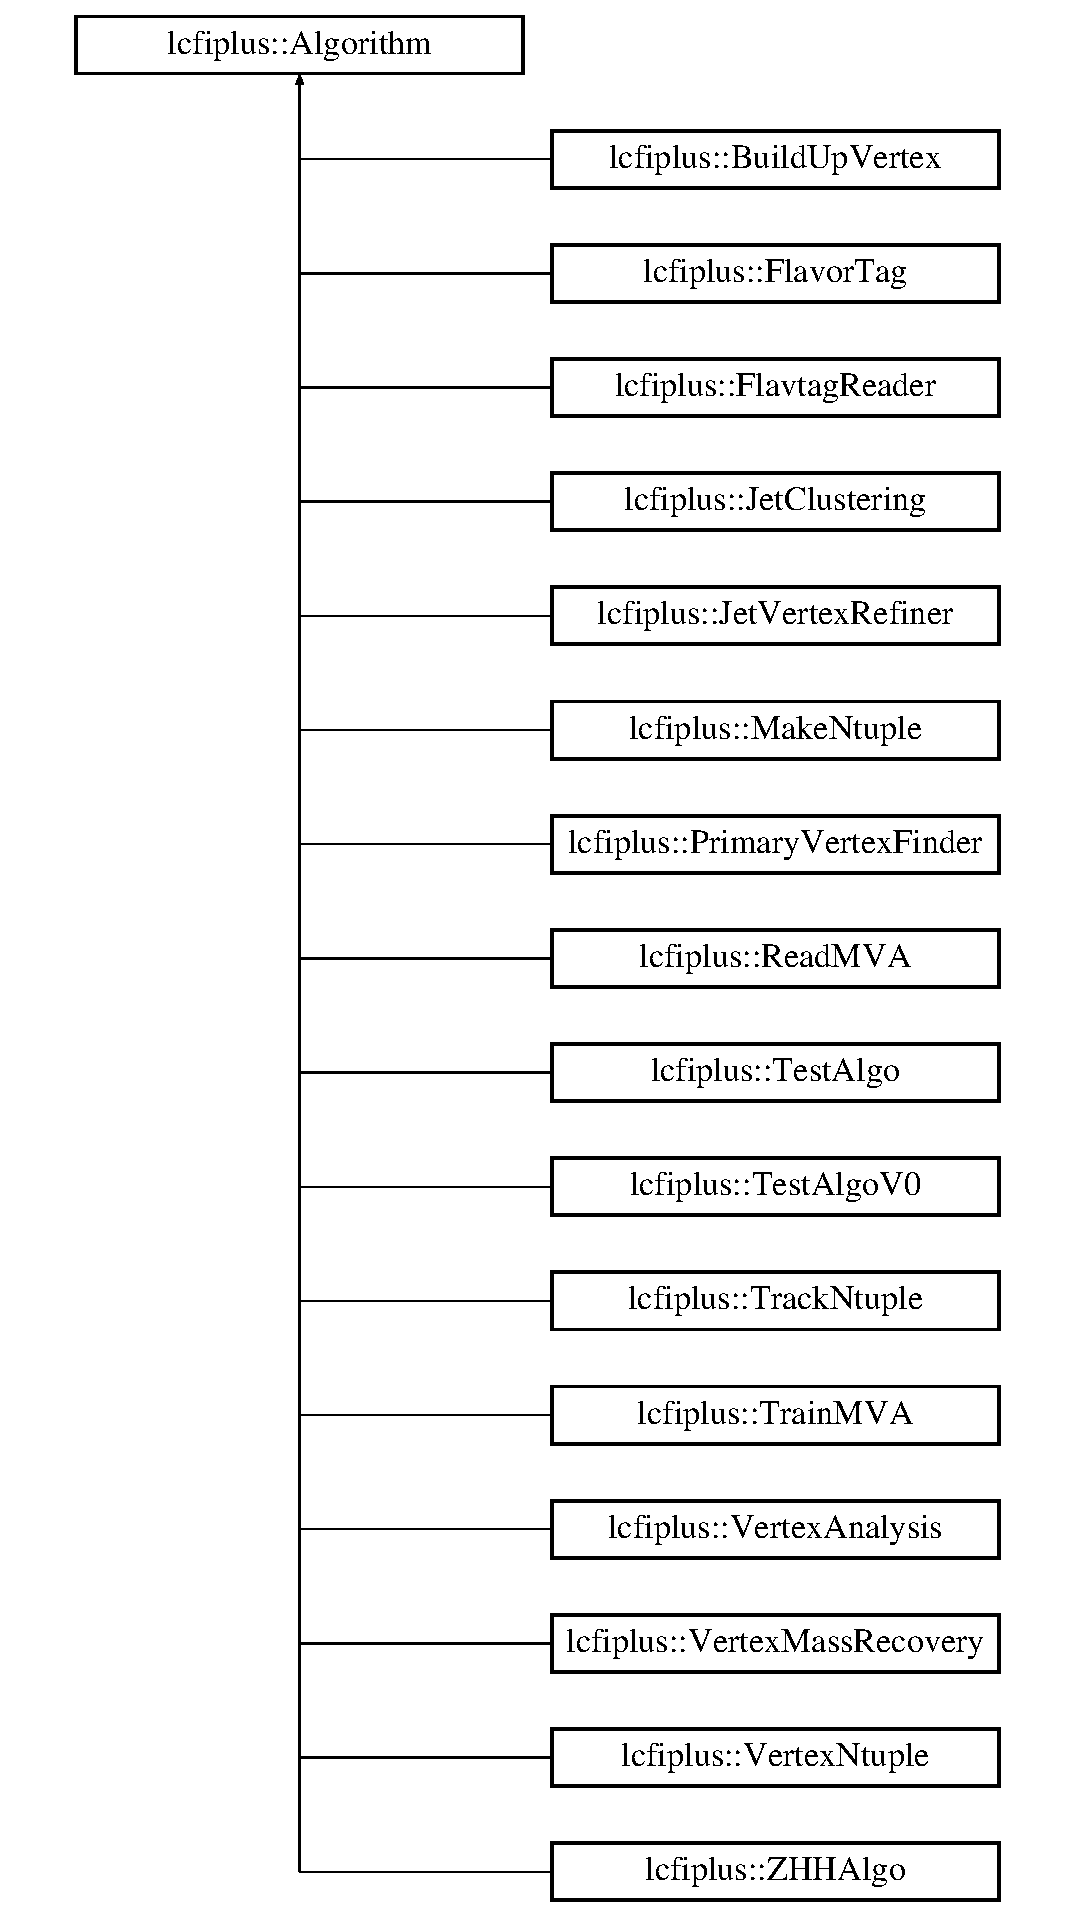
\includegraphics[height=12.000000cm]{classlcfiplus_1_1Algorithm}
\end{center}
\end{figure}
\subsection*{Public Member Functions}
\begin{DoxyCompactItemize}
\item 
{\bf Algorithm} ()
\item 
virtual {\bf $\sim$\-Algorithm} ()
\item 
virtual void {\bf init} ({\bf Parameters} $\ast$param)
\item 
virtual void {\bf process} ()=0
\item 
virtual void {\bf end} ()
\end{DoxyCompactItemize}
\subsection*{Protected Member Functions}
\begin{DoxyCompactItemize}
\item 
{\bf Parameters} $\ast$ {\bf Get\-Param} () const 
\end{DoxyCompactItemize}


\subsection{Constructor \& Destructor Documentation}
\index{lcfiplus\-::\-Algorithm@{lcfiplus\-::\-Algorithm}!Algorithm@{Algorithm}}
\index{Algorithm@{Algorithm}!lcfiplus::Algorithm@{lcfiplus\-::\-Algorithm}}
\subsubsection[{Algorithm}]{\setlength{\rightskip}{0pt plus 5cm}lcfiplus\-::\-Algorithm\-::\-Algorithm (
\begin{DoxyParamCaption}
{}
\end{DoxyParamCaption}
)\hspace{0.3cm}{\ttfamily [inline]}}\label{classlcfiplus_1_1Algorithm_a3ff0f3c83b0c0d19bf0f0e8046fc889f}
\index{lcfiplus\-::\-Algorithm@{lcfiplus\-::\-Algorithm}!$\sim$\-Algorithm@{$\sim$\-Algorithm}}
\index{$\sim$\-Algorithm@{$\sim$\-Algorithm}!lcfiplus::Algorithm@{lcfiplus\-::\-Algorithm}}
\subsubsection[{$\sim$\-Algorithm}]{\setlength{\rightskip}{0pt plus 5cm}virtual lcfiplus\-::\-Algorithm\-::$\sim$\-Algorithm (
\begin{DoxyParamCaption}
{}
\end{DoxyParamCaption}
)\hspace{0.3cm}{\ttfamily [inline]}, {\ttfamily [virtual]}}\label{classlcfiplus_1_1Algorithm_a17b9d587d638ed6c29e12141e24d8648}


\subsection{Member Function Documentation}
\index{lcfiplus\-::\-Algorithm@{lcfiplus\-::\-Algorithm}!end@{end}}
\index{end@{end}!lcfiplus::Algorithm@{lcfiplus\-::\-Algorithm}}
\subsubsection[{end}]{\setlength{\rightskip}{0pt plus 5cm}virtual void lcfiplus\-::\-Algorithm\-::end (
\begin{DoxyParamCaption}
{}
\end{DoxyParamCaption}
)\hspace{0.3cm}{\ttfamily [inline]}, {\ttfamily [virtual]}}\label{classlcfiplus_1_1Algorithm_a4276b93869d614f59eef92b8c728ef60}


Reimplemented in {\bf lcfiplus\-::\-Test\-Algo\-V0} \doxyref{}{p.}{classlcfiplus_1_1TestAlgoV0_a4a2881e2da193e7ca54f520be8da24a4}, {\bf lcfiplus\-::\-Flavtag\-Reader} \doxyref{}{p.}{classlcfiplus_1_1FlavtagReader_a6b4aeb451123b3fa850a24730f0f12b7}, {\bf lcfiplus\-::\-Vertex\-Analysis} \doxyref{}{p.}{classlcfiplus_1_1VertexAnalysis_ae285c0bf92e2c632214e4a04d8a87198}, {\bf lcfiplus\-::\-Test\-Algo} \doxyref{}{p.}{classlcfiplus_1_1TestAlgo_ac9c6e715440d0af7cdbb661f6c4bf20d}, {\bf lcfiplus\-::\-Z\-H\-H\-Algo} \doxyref{}{p.}{classlcfiplus_1_1ZHHAlgo_a58e42be74da0dccdfe74242abaf6aa35}, {\bf lcfiplus\-::\-Jet\-Vertex\-Refiner} \doxyref{}{p.}{classlcfiplus_1_1JetVertexRefiner_adc79802a860e580b8abd29587eb12e52}, {\bf lcfiplus\-::\-Jet\-Clustering} \doxyref{}{p.}{classlcfiplus_1_1JetClustering_abdf958641bff23a9b698246dc75f53e7}, {\bf lcfiplus\-::\-Build\-Up\-Vertex} \doxyref{}{p.}{classlcfiplus_1_1BuildUpVertex_a767da73886af74b8dc491128b2caa47e}, {\bf lcfiplus\-::\-Flavor\-Tag} \doxyref{}{p.}{classlcfiplus_1_1FlavorTag_abd9ac826b60d9c51d3ed8d7cf02de074}, {\bf lcfiplus\-::\-Read\-M\-V\-A} \doxyref{}{p.}{classlcfiplus_1_1ReadMVA_a897b05f08ac46041c404391c12c9d41c}, {\bf lcfiplus\-::\-Track\-Ntuple} \doxyref{}{p.}{classlcfiplus_1_1TrackNtuple_ab940f0c564373201bd99f64592e6c69e}, {\bf lcfiplus\-::\-Train\-M\-V\-A} \doxyref{}{p.}{classlcfiplus_1_1TrainMVA_afc76d99754235fdcefd3e02bc39b49f2}, {\bf lcfiplus\-::\-Vertex\-Ntuple} \doxyref{}{p.}{classlcfiplus_1_1VertexNtuple_ab14aa51a6f3bf65b13663a5f8e081082}, {\bf lcfiplus\-::\-Make\-Ntuple} \doxyref{}{p.}{classlcfiplus_1_1MakeNtuple_a7e06f982e158316c2b952a14c04c059e}, {\bf lcfiplus\-::\-Primary\-Vertex\-Finder} \doxyref{}{p.}{classlcfiplus_1_1PrimaryVertexFinder_ad58d2554a7ce1e34c5994f45fa692b0f}, and {\bf lcfiplus\-::\-Vertex\-Mass\-Recovery} \doxyref{}{p.}{classlcfiplus_1_1VertexMassRecovery_aed7fc11a47fdef3f6db157db9a6b5327}.

\index{lcfiplus\-::\-Algorithm@{lcfiplus\-::\-Algorithm}!Get\-Param@{Get\-Param}}
\index{Get\-Param@{Get\-Param}!lcfiplus::Algorithm@{lcfiplus\-::\-Algorithm}}
\subsubsection[{Get\-Param}]{\setlength{\rightskip}{0pt plus 5cm}{\bf Parameters}$\ast$ lcfiplus\-::\-Algorithm\-::\-Get\-Param (
\begin{DoxyParamCaption}
{}
\end{DoxyParamCaption}
) const\hspace{0.3cm}{\ttfamily [inline]}, {\ttfamily [protected]}}\label{classlcfiplus_1_1Algorithm_a0e009e457a811b2f22c5843620c084b9}
\index{lcfiplus\-::\-Algorithm@{lcfiplus\-::\-Algorithm}!init@{init}}
\index{init@{init}!lcfiplus::Algorithm@{lcfiplus\-::\-Algorithm}}
\subsubsection[{init}]{\setlength{\rightskip}{0pt plus 5cm}virtual void lcfiplus\-::\-Algorithm\-::init (
\begin{DoxyParamCaption}
\item[{{\bf Parameters} $\ast$}]{param}
\end{DoxyParamCaption}
)\hspace{0.3cm}{\ttfamily [inline]}, {\ttfamily [virtual]}}\label{classlcfiplus_1_1Algorithm_a178a273b9976b87f182190f4250cac9e}


Reimplemented in {\bf lcfiplus\-::\-Test\-Algo\-V0} \doxyref{}{p.}{classlcfiplus_1_1TestAlgoV0_ad780aabe2ebca9cb0cad56a2a673cdfc}, {\bf lcfiplus\-::\-Flavtag\-Reader} \doxyref{}{p.}{classlcfiplus_1_1FlavtagReader_a5b72270f230113bf33924453f8149fed}, {\bf lcfiplus\-::\-Vertex\-Analysis} \doxyref{}{p.}{classlcfiplus_1_1VertexAnalysis_a298dba341823b2dc2f3dd43aac75e5e5}, {\bf lcfiplus\-::\-Test\-Algo} \doxyref{}{p.}{classlcfiplus_1_1TestAlgo_af7e0164303961e996f0ee3f69dab9892}, {\bf lcfiplus\-::\-Z\-H\-H\-Algo} \doxyref{}{p.}{classlcfiplus_1_1ZHHAlgo_a2f2b4bd1296077c157067c6d16ec7f0b}, {\bf lcfiplus\-::\-Jet\-Vertex\-Refiner} \doxyref{}{p.}{classlcfiplus_1_1JetVertexRefiner_aef1b5ffa8ef2742d6a5c74171152f746}, {\bf lcfiplus\-::\-Jet\-Clustering} \doxyref{}{p.}{classlcfiplus_1_1JetClustering_a07261e0f55daccd2e26d720079e8831f}, {\bf lcfiplus\-::\-Build\-Up\-Vertex} \doxyref{}{p.}{classlcfiplus_1_1BuildUpVertex_a6bb5e0d748b385389332c3f3ddd4d054}, {\bf lcfiplus\-::\-Flavor\-Tag} \doxyref{}{p.}{classlcfiplus_1_1FlavorTag_aa872596e47fd0e4ac56b70e144d9408e}, {\bf lcfiplus\-::\-Read\-M\-V\-A} \doxyref{}{p.}{classlcfiplus_1_1ReadMVA_a14c659f3c03cead1f981302e1ff46496}, {\bf lcfiplus\-::\-Track\-Ntuple} \doxyref{}{p.}{classlcfiplus_1_1TrackNtuple_a8bfc0c42c42575aeac6969cdccb4358c}, {\bf lcfiplus\-::\-Train\-M\-V\-A} \doxyref{}{p.}{classlcfiplus_1_1TrainMVA_a95ad4f6ac7ee75c9376d46399ec7c41f}, {\bf lcfiplus\-::\-Vertex\-Ntuple} \doxyref{}{p.}{classlcfiplus_1_1VertexNtuple_a0af57e769fd35613fcd348271b870c82}, {\bf lcfiplus\-::\-Make\-Ntuple} \doxyref{}{p.}{classlcfiplus_1_1MakeNtuple_aa7aaff1c8fb3f13047fe5fcd2220b2df}, {\bf lcfiplus\-::\-Primary\-Vertex\-Finder} \doxyref{}{p.}{classlcfiplus_1_1PrimaryVertexFinder_a6c53ee4057ba9f3fc6790732f908ad2b}, and {\bf lcfiplus\-::\-Vertex\-Mass\-Recovery} \doxyref{}{p.}{classlcfiplus_1_1VertexMassRecovery_aff886b65ff0988e46797c9bb631bdc3d}.



Referenced by lcfiplus\-::\-Vertex\-Mass\-Recovery\-::init(), lcfiplus\-::\-Primary\-Vertex\-Finder\-::init(), lcfiplus\-::\-Make\-Ntuple\-::init(), lcfiplus\-::\-Vertex\-Ntuple\-::init(), lcfiplus\-::\-Train\-M\-V\-A\-::init(), lcfiplus\-::\-Read\-M\-V\-A\-::init(), lcfiplus\-::\-Track\-Ntuple\-::init(), lcfiplus\-::\-Flavor\-Tag\-::init(), Lcfiplus\-Processor\-::init(), lcfiplus\-::\-Build\-Up\-Vertex\-::init(), lcfiplus\-::\-Jet\-Clustering\-::init(), lcfiplus\-::\-Jet\-Vertex\-Refiner\-::init(), lcfiplus\-::\-Z\-H\-H\-Algo\-::init(), lcfiplus\-::\-Test\-Algo\-::init(), lcfiplus\-::\-Vertex\-Analysis\-::init(), lcfiplus\-::\-Flavtag\-Reader\-::init(), and lcfiplus\-::\-Test\-Algo\-V0\-::init().

\index{lcfiplus\-::\-Algorithm@{lcfiplus\-::\-Algorithm}!process@{process}}
\index{process@{process}!lcfiplus::Algorithm@{lcfiplus\-::\-Algorithm}}
\subsubsection[{process}]{\setlength{\rightskip}{0pt plus 5cm}virtual void lcfiplus\-::\-Algorithm\-::process (
\begin{DoxyParamCaption}
{}
\end{DoxyParamCaption}
)\hspace{0.3cm}{\ttfamily [pure virtual]}}\label{classlcfiplus_1_1Algorithm_a628e1509b55b2cda1e2640b58be6ce6f}


Implemented in {\bf lcfiplus\-::\-Test\-Algo\-V0} \doxyref{}{p.}{classlcfiplus_1_1TestAlgoV0_a33a852d925ad190d5c3a8fe9e017897a}, {\bf lcfiplus\-::\-Flavtag\-Reader} \doxyref{}{p.}{classlcfiplus_1_1FlavtagReader_a7cd1aca9d0bd08130f8f965de9fdaed7}, {\bf lcfiplus\-::\-Vertex\-Analysis} \doxyref{}{p.}{classlcfiplus_1_1VertexAnalysis_a7b3b72ff956a5363ad3b8a837963afdc}, {\bf lcfiplus\-::\-Test\-Algo} \doxyref{}{p.}{classlcfiplus_1_1TestAlgo_acd0209c2dfb0ffe063602aa48961fd76}, {\bf lcfiplus\-::\-Z\-H\-H\-Algo} \doxyref{}{p.}{classlcfiplus_1_1ZHHAlgo_ac9fcb369c4cd73fef59d13bc5d9ebfb2}, {\bf lcfiplus\-::\-Jet\-Vertex\-Refiner} \doxyref{}{p.}{classlcfiplus_1_1JetVertexRefiner_a082fc532079e624db382fa9615cda990}, {\bf lcfiplus\-::\-Jet\-Clustering} \doxyref{}{p.}{classlcfiplus_1_1JetClustering_ac526918c0b75934cb1a6f8d72d97fa17}, {\bf lcfiplus\-::\-Build\-Up\-Vertex} \doxyref{}{p.}{classlcfiplus_1_1BuildUpVertex_a0d0f0a9f8e04a99b117ca0019c0df5a6}, {\bf lcfiplus\-::\-Flavor\-Tag} \doxyref{}{p.}{classlcfiplus_1_1FlavorTag_a44be9eb8162b2daabd06907c39098d33}, {\bf lcfiplus\-::\-Read\-M\-V\-A} \doxyref{}{p.}{classlcfiplus_1_1ReadMVA_a71eb4cee7adb1cf0a8bbe94f28896a56}, {\bf lcfiplus\-::\-Track\-Ntuple} \doxyref{}{p.}{classlcfiplus_1_1TrackNtuple_ae1e651a4d89e27ce1b104584ed271407}, {\bf lcfiplus\-::\-Train\-M\-V\-A} \doxyref{}{p.}{classlcfiplus_1_1TrainMVA_acc285782d7c12ad41688f0ecb9e7bbd1}, {\bf lcfiplus\-::\-Vertex\-Ntuple} \doxyref{}{p.}{classlcfiplus_1_1VertexNtuple_a44ce611e99b7e130e16a49948826bca0}, {\bf lcfiplus\-::\-Make\-Ntuple} \doxyref{}{p.}{classlcfiplus_1_1MakeNtuple_a3d48fa43fa7e63c57ae4bbac7cca7fd4}, {\bf lcfiplus\-::\-Primary\-Vertex\-Finder} \doxyref{}{p.}{classlcfiplus_1_1PrimaryVertexFinder_a04fd64dc5fea42a47159195dfe264b4b}, and {\bf lcfiplus\-::\-Vertex\-Mass\-Recovery} \doxyref{}{p.}{classlcfiplus_1_1VertexMassRecovery_aaada66e1654328e8c3fafa59573d14fb}.



The documentation for this class was generated from the following file\-:\begin{DoxyCompactItemize}
\item 
{\bf lcfiplus.\-h}\end{DoxyCompactItemize}

\section{lcfiplus\-:\-:Build\-Up\-Vertex Class Reference}
\label{classlcfiplus_1_1BuildUpVertex}\index{lcfiplus\-::\-Build\-Up\-Vertex@{lcfiplus\-::\-Build\-Up\-Vertex}}


{\ttfamily \#include $<$process.\-h$>$}

Inheritance diagram for lcfiplus\-:\-:Build\-Up\-Vertex\-:\begin{figure}[H]
\begin{center}
\leavevmode
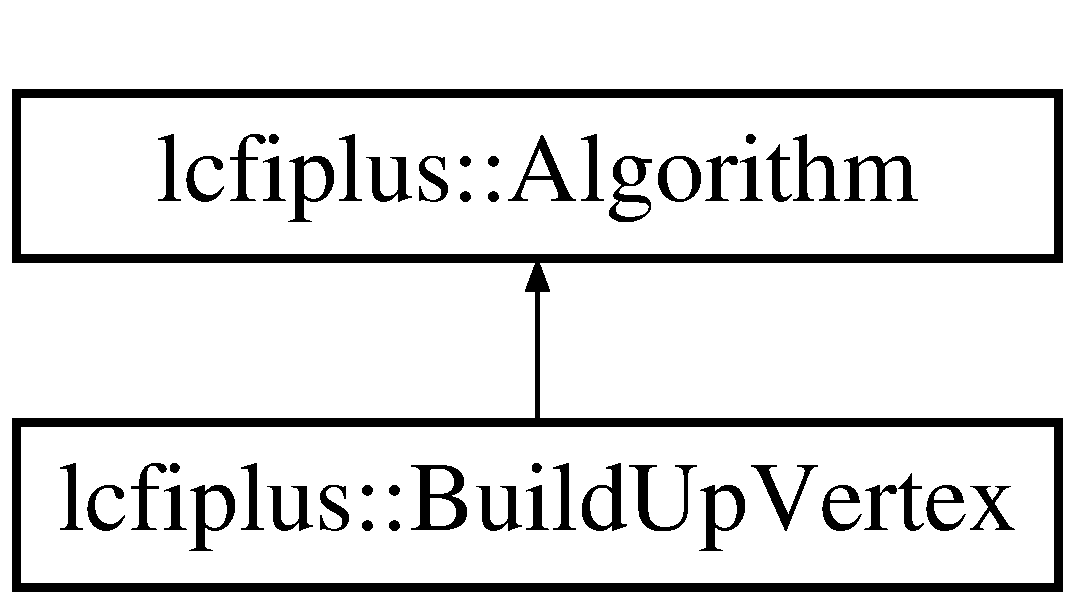
\includegraphics[height=2.000000cm]{classlcfiplus_1_1BuildUpVertex}
\end{center}
\end{figure}
\subsection*{Public Member Functions}
\begin{DoxyCompactItemize}
\item 
{\bf Build\-Up\-Vertex} ()
\item 
virtual {\bf $\sim$\-Build\-Up\-Vertex} ()
\item 
void {\bf init} ({\bf Parameters} $\ast$param)
\item 
void {\bf process} ()
\item 
void {\bf end} ()
\item 
{\bf Class\-Def} ({\bf Build\-Up\-Vertex}, 1)
\end{DoxyCompactItemize}
\subsection*{Additional Inherited Members}


\subsection{Constructor \& Destructor Documentation}
\index{lcfiplus\-::\-Build\-Up\-Vertex@{lcfiplus\-::\-Build\-Up\-Vertex}!Build\-Up\-Vertex@{Build\-Up\-Vertex}}
\index{Build\-Up\-Vertex@{Build\-Up\-Vertex}!lcfiplus::BuildUpVertex@{lcfiplus\-::\-Build\-Up\-Vertex}}
\subsubsection[{Build\-Up\-Vertex}]{\setlength{\rightskip}{0pt plus 5cm}lcfiplus\-::\-Build\-Up\-Vertex\-::\-Build\-Up\-Vertex (
\begin{DoxyParamCaption}
{}
\end{DoxyParamCaption}
)\hspace{0.3cm}{\ttfamily [inline]}}\label{classlcfiplus_1_1BuildUpVertex_af14eaf4285e87dada2a57260f3d25793}
\index{lcfiplus\-::\-Build\-Up\-Vertex@{lcfiplus\-::\-Build\-Up\-Vertex}!$\sim$\-Build\-Up\-Vertex@{$\sim$\-Build\-Up\-Vertex}}
\index{$\sim$\-Build\-Up\-Vertex@{$\sim$\-Build\-Up\-Vertex}!lcfiplus::BuildUpVertex@{lcfiplus\-::\-Build\-Up\-Vertex}}
\subsubsection[{$\sim$\-Build\-Up\-Vertex}]{\setlength{\rightskip}{0pt plus 5cm}virtual lcfiplus\-::\-Build\-Up\-Vertex\-::$\sim$\-Build\-Up\-Vertex (
\begin{DoxyParamCaption}
{}
\end{DoxyParamCaption}
)\hspace{0.3cm}{\ttfamily [inline]}, {\ttfamily [virtual]}}\label{classlcfiplus_1_1BuildUpVertex_a524d7aa3c6cc41558d788a8d13520de6}


\subsection{Member Function Documentation}
\index{lcfiplus\-::\-Build\-Up\-Vertex@{lcfiplus\-::\-Build\-Up\-Vertex}!Class\-Def@{Class\-Def}}
\index{Class\-Def@{Class\-Def}!lcfiplus::BuildUpVertex@{lcfiplus\-::\-Build\-Up\-Vertex}}
\subsubsection[{Class\-Def}]{\setlength{\rightskip}{0pt plus 5cm}lcfiplus\-::\-Build\-Up\-Vertex\-::\-Class\-Def (
\begin{DoxyParamCaption}
\item[{{\bf Build\-Up\-Vertex}}]{, }
\item[{1}]{}
\end{DoxyParamCaption}
)}\label{classlcfiplus_1_1BuildUpVertex_a070df65953d2552a613588e60e3ea95d}
\index{lcfiplus\-::\-Build\-Up\-Vertex@{lcfiplus\-::\-Build\-Up\-Vertex}!end@{end}}
\index{end@{end}!lcfiplus::BuildUpVertex@{lcfiplus\-::\-Build\-Up\-Vertex}}
\subsubsection[{end}]{\setlength{\rightskip}{0pt plus 5cm}void lcfiplus\-::\-Build\-Up\-Vertex\-::end (
\begin{DoxyParamCaption}
{}
\end{DoxyParamCaption}
)\hspace{0.3cm}{\ttfamily [virtual]}}\label{classlcfiplus_1_1BuildUpVertex_a767da73886af74b8dc491128b2caa47e}


Reimplemented from {\bf lcfiplus\-::\-Algorithm} \doxyref{}{p.}{classlcfiplus_1_1Algorithm_a4276b93869d614f59eef92b8c728ef60}.

\index{lcfiplus\-::\-Build\-Up\-Vertex@{lcfiplus\-::\-Build\-Up\-Vertex}!init@{init}}
\index{init@{init}!lcfiplus::BuildUpVertex@{lcfiplus\-::\-Build\-Up\-Vertex}}
\subsubsection[{init}]{\setlength{\rightskip}{0pt plus 5cm}void lcfiplus\-::\-Build\-Up\-Vertex\-::init (
\begin{DoxyParamCaption}
\item[{{\bf Parameters} $\ast$}]{param}
\end{DoxyParamCaption}
)\hspace{0.3cm}{\ttfamily [virtual]}}\label{classlcfiplus_1_1BuildUpVertex_a6bb5e0d748b385389332c3f3ddd4d054}


Reimplemented from {\bf lcfiplus\-::\-Algorithm} \doxyref{}{p.}{classlcfiplus_1_1Algorithm_a178a273b9976b87f182190f4250cac9e}.



References lcfiplus\-::\-Parameters\-::get(), lcfiplus\-::\-Algorithm\-::init(), lcfiplus\-::\-Event\-::\-Instance(), lcfiplus\-::\-Track\-Selector\-Config\-::max\-D0, lcfiplus\-::\-Event\-Store\-::\-P\-E\-R\-S\-I\-S\-T, lcfiplus\-::\-Event\-Store\-::\-Register(), and lcfiplus\-::\-Event\-::set\-Default\-Primary\-Vertex().

\index{lcfiplus\-::\-Build\-Up\-Vertex@{lcfiplus\-::\-Build\-Up\-Vertex}!process@{process}}
\index{process@{process}!lcfiplus::BuildUpVertex@{lcfiplus\-::\-Build\-Up\-Vertex}}
\subsubsection[{process}]{\setlength{\rightskip}{0pt plus 5cm}void lcfiplus\-::\-Build\-Up\-Vertex\-::process (
\begin{DoxyParamCaption}
{}
\end{DoxyParamCaption}
)\hspace{0.3cm}{\ttfamily [virtual]}}\label{classlcfiplus_1_1BuildUpVertex_a0d0f0a9f8e04a99b117ca0019c0df5a6}


Implements {\bf lcfiplus\-::\-Algorithm} \doxyref{}{p.}{classlcfiplus_1_1Algorithm_a628e1509b55b2cda1e2640b58be6ce6f}.



References lcfiplus\-::\-Vertex\-Finder\-Suehara\-::associate\-I\-P\-Tracks(), lcfiplus\-::\-Vertex\-Finder\-Suehara\-::associate\-I\-P\-Tracks\-A\-V\-F(), lcfiplus\-::\-Vertex\-Finder\-Suehara\-::\-Vertex\-Finder\-Suehara\-Config\-::avf, lcfiplus\-::\-Vertex\-Finder\-Suehara\-::build\-Up(), lcfiplus\-::\-Vertex\-Finder\-Suehara\-::\-Vertex\-Finder\-Suehara\-Config\-::chi2orderinglimit, lcfiplus\-::\-Vertex\-Finder\-Suehara\-::\-Vertex\-Finder\-Suehara\-Config\-::chi2ratio\-I\-P, lcfiplus\-::\-Vertex\-Finder\-Suehara\-::\-Vertex\-Finder\-Suehara\-Config\-::chi2th, lcfiplus\-::\-Event\-Store\-::\-Get(), lcfiplus\-::\-Vertex\-::get\-Tracks(), lcfiplus\-::\-Event\-::\-Instance(), lcfiplus\-::\-Vertex\-Finder\-Suehara\-::\-Vertex\-Finder\-Suehara\-Config\-::massth, lcfiplus\-::\-Vertex\-Finder\-Suehara\-::\-Vertex\-Finder\-Suehara\-Config\-::minimumdist\-I\-P, lcfiplus\-::\-Vertex\-Selector\-Config\-::minpos, lcfiplus\-::\-Vertex\-Selector\-Config\-::set\-No\-V0\-Cut(), lcfiplus\-::\-Vertex\-Finder\-Suehara\-::\-Vertex\-Finder\-Suehara\-Config\-::temperature, lcfiplus\-::\-Vertex\-Finder\-Suehara\-::\-Vertex\-Finder\-Suehara\-Config\-::v0sel\-Track, and lcfiplus\-::\-Vertex\-Finder\-Suehara\-::\-Vertex\-Finder\-Suehara\-Config\-::v0sel\-Vertex.



The documentation for this class was generated from the following files\-:\begin{DoxyCompactItemize}
\item 
{\bf process.\-h}\item 
{\bf process.\-cc}\end{DoxyCompactItemize}

\section{lcfiplus\-:\-:Z\-H\-H\-Algo\-:\-:data Struct Reference}
\label{structlcfiplus_1_1ZHHAlgo_1_1data}\index{lcfiplus\-::\-Z\-H\-H\-Algo\-::data@{lcfiplus\-::\-Z\-H\-H\-Algo\-::data}}


{\ttfamily \#include $<$testproc.\-h$>$}

\subsection*{Public Attributes}
\begin{DoxyCompactItemize}
\item 
int {\bf mchdecaypdg} [2]
\item 
int {\bf mchbb}
\item 
int {\bf mcnb}
\item 
double {\bf thrust}
\item 
double {\bf thaxis} [3]
\item 
double {\bf ycuts} [10]
\item 
int {\bf ntr}
\item 
int {\bf npfo}
\item 
double {\bf mass} [15]
\item 
double {\bf ntrjetmin}
\item 
double {\bf pmiss} [3]
\item 
double {\bf emiss}
\item 
double {\bf bcat} [6]
\item 
double {\bf btag} [6]
\item 
double {\bf ctag} [6]
\item 
double {\bf ejet} [6]
\item 
double {\bf pxjet} [6]
\item 
double {\bf pyjet} [6]
\item 
double {\bf pzjet} [6]
\item 
double {\bf ntrjet} [6]
\item 
double {\bf twovtxprobjet} [6]
\item 
double {\bf vtxangle} [6]
\item 
double {\bf mcnb6} [6]
\item 
double {\bf mcnc6} [6]
\item 
double {\bf bcat4} [4]
\item 
double {\bf btag4} [4]
\item 
double {\bf ctag4} [4]
\item 
double {\bf ejet4} [4]
\item 
double {\bf pxjet4} [4]
\item 
double {\bf pyjet4} [4]
\item 
double {\bf pzjet4} [4]
\item 
double {\bf ntrjet4} [4]
\item 
double {\bf twovtxprobjet4} [4]
\item 
double {\bf vtxangle4} [4]
\item 
double {\bf bcat5} [5]
\item 
double {\bf btag5} [5]
\item 
double {\bf ctag5} [5]
\item 
double {\bf ejet5} [5]
\item 
double {\bf pxjet5} [5]
\item 
double {\bf pyjet5} [5]
\item 
double {\bf pzjet5} [5]
\item 
double {\bf ntrjet5} [5]
\item 
double {\bf twovtxprobjet5} [5]
\item 
double {\bf vtxangle5} [5]
\item 
double {\bf bcat7} [7]
\item 
double {\bf btag7} [7]
\item 
double {\bf ctag7} [7]
\item 
double {\bf ejet7} [7]
\item 
double {\bf pxjet7} [7]
\item 
double {\bf pyjet7} [7]
\item 
double {\bf pzjet7} [7]
\item 
double {\bf ntrjet7} [7]
\item 
double {\bf twovtxprobjet7} [7]
\item 
double {\bf vtxangle7} [7]
\item 
double {\bf bcat8} [8]
\item 
double {\bf btag8} [8]
\item 
double {\bf ctag8} [8]
\item 
double {\bf ejet8} [8]
\item 
double {\bf pxjet8} [8]
\item 
double {\bf pyjet8} [8]
\item 
double {\bf pzjet8} [8]
\item 
double {\bf ntrjet8} [8]
\item 
double {\bf twovtxprobjet8} [8]
\item 
double {\bf vtxangle8} [8]
\item 
double {\bf bcatnv4} [4]
\item 
double {\bf btagnv4} [4]
\item 
double {\bf ctagnv4} [4]
\item 
double {\bf ejetnv4} [4]
\item 
double {\bf pxjetnv4} [4]
\item 
double {\bf pyjetnv4} [4]
\item 
double {\bf pzjetnv4} [4]
\item 
double {\bf ntrjetnv4} [4]
\item 
double {\bf twovtxprobjetnv4} [4]
\item 
double {\bf vtxanglenv4} [4]
\item 
double {\bf bcatnv5} [5]
\item 
double {\bf btagnv5} [5]
\item 
double {\bf ctagnv5} [5]
\item 
double {\bf ejetnv5} [5]
\item 
double {\bf pxjetnv5} [5]
\item 
double {\bf pyjetnv5} [5]
\item 
double {\bf pzjetnv5} [5]
\item 
double {\bf ntrjetnv5} [5]
\item 
double {\bf twovtxprobjetnv5} [5]
\item 
double {\bf vtxanglenv5} [5]
\item 
double {\bf bcatnv6} [6]
\item 
double {\bf btagnv6} [6]
\item 
double {\bf ctagnv6} [6]
\item 
double {\bf ejetnv6} [6]
\item 
double {\bf pxjetnv6} [6]
\item 
double {\bf pyjetnv6} [6]
\item 
double {\bf pzjetnv6} [6]
\item 
double {\bf ntrjetnv6} [6]
\item 
double {\bf twovtxprobjetnv6} [6]
\item 
double {\bf vtxanglenv6} [6]
\item 
double {\bf bcatnv7} [7]
\item 
double {\bf btagnv7} [7]
\item 
double {\bf ctagnv7} [7]
\item 
double {\bf ejetnv7} [7]
\item 
double {\bf pxjetnv7} [7]
\item 
double {\bf pyjetnv7} [7]
\item 
double {\bf pzjetnv7} [7]
\item 
double {\bf ntrjetnv7} [7]
\item 
double {\bf twovtxprobjetnv7} [7]
\item 
double {\bf vtxanglenv7} [7]
\item 
double {\bf bcatnv8} [8]
\item 
double {\bf btagnv8} [8]
\item 
double {\bf ctagnv8} [8]
\item 
double {\bf ejetnv8} [8]
\item 
double {\bf pxjetnv8} [8]
\item 
double {\bf pyjetnv8} [8]
\item 
double {\bf pzjetnv8} [8]
\item 
double {\bf ntrjetnv8} [8]
\item 
double {\bf twovtxprobjetnv8} [8]
\item 
double {\bf vtxanglenv8} [8]
\end{DoxyCompactItemize}


\subsection{Member Data Documentation}
\index{lcfiplus\-::\-Z\-H\-H\-Algo\-::data@{lcfiplus\-::\-Z\-H\-H\-Algo\-::data}!bcat@{bcat}}
\index{bcat@{bcat}!lcfiplus::ZHHAlgo::data@{lcfiplus\-::\-Z\-H\-H\-Algo\-::data}}
\subsubsection[{bcat}]{\setlength{\rightskip}{0pt plus 5cm}double lcfiplus\-::\-Z\-H\-H\-Algo\-::data\-::bcat[6]}\label{structlcfiplus_1_1ZHHAlgo_1_1data_a6fcb9ce285bf3d4533e2561169457f2f}
\index{lcfiplus\-::\-Z\-H\-H\-Algo\-::data@{lcfiplus\-::\-Z\-H\-H\-Algo\-::data}!bcat4@{bcat4}}
\index{bcat4@{bcat4}!lcfiplus::ZHHAlgo::data@{lcfiplus\-::\-Z\-H\-H\-Algo\-::data}}
\subsubsection[{bcat4}]{\setlength{\rightskip}{0pt plus 5cm}double lcfiplus\-::\-Z\-H\-H\-Algo\-::data\-::bcat4[4]}\label{structlcfiplus_1_1ZHHAlgo_1_1data_a752d7d257df5cade66beffad42c5e522}
\index{lcfiplus\-::\-Z\-H\-H\-Algo\-::data@{lcfiplus\-::\-Z\-H\-H\-Algo\-::data}!bcat5@{bcat5}}
\index{bcat5@{bcat5}!lcfiplus::ZHHAlgo::data@{lcfiplus\-::\-Z\-H\-H\-Algo\-::data}}
\subsubsection[{bcat5}]{\setlength{\rightskip}{0pt plus 5cm}double lcfiplus\-::\-Z\-H\-H\-Algo\-::data\-::bcat5[5]}\label{structlcfiplus_1_1ZHHAlgo_1_1data_a29ac8539d5d9f00472fcbaceaecadb29}
\index{lcfiplus\-::\-Z\-H\-H\-Algo\-::data@{lcfiplus\-::\-Z\-H\-H\-Algo\-::data}!bcat7@{bcat7}}
\index{bcat7@{bcat7}!lcfiplus::ZHHAlgo::data@{lcfiplus\-::\-Z\-H\-H\-Algo\-::data}}
\subsubsection[{bcat7}]{\setlength{\rightskip}{0pt plus 5cm}double lcfiplus\-::\-Z\-H\-H\-Algo\-::data\-::bcat7[7]}\label{structlcfiplus_1_1ZHHAlgo_1_1data_a1e528fa8bf997c21f9001ae551d13f7c}
\index{lcfiplus\-::\-Z\-H\-H\-Algo\-::data@{lcfiplus\-::\-Z\-H\-H\-Algo\-::data}!bcat8@{bcat8}}
\index{bcat8@{bcat8}!lcfiplus::ZHHAlgo::data@{lcfiplus\-::\-Z\-H\-H\-Algo\-::data}}
\subsubsection[{bcat8}]{\setlength{\rightskip}{0pt plus 5cm}double lcfiplus\-::\-Z\-H\-H\-Algo\-::data\-::bcat8[8]}\label{structlcfiplus_1_1ZHHAlgo_1_1data_aa65dc5aa9a40d1de5056c561ab22d289}
\index{lcfiplus\-::\-Z\-H\-H\-Algo\-::data@{lcfiplus\-::\-Z\-H\-H\-Algo\-::data}!bcatnv4@{bcatnv4}}
\index{bcatnv4@{bcatnv4}!lcfiplus::ZHHAlgo::data@{lcfiplus\-::\-Z\-H\-H\-Algo\-::data}}
\subsubsection[{bcatnv4}]{\setlength{\rightskip}{0pt plus 5cm}double lcfiplus\-::\-Z\-H\-H\-Algo\-::data\-::bcatnv4[4]}\label{structlcfiplus_1_1ZHHAlgo_1_1data_aab0f82f6feba9621b6430c2792e3a2bd}
\index{lcfiplus\-::\-Z\-H\-H\-Algo\-::data@{lcfiplus\-::\-Z\-H\-H\-Algo\-::data}!bcatnv5@{bcatnv5}}
\index{bcatnv5@{bcatnv5}!lcfiplus::ZHHAlgo::data@{lcfiplus\-::\-Z\-H\-H\-Algo\-::data}}
\subsubsection[{bcatnv5}]{\setlength{\rightskip}{0pt plus 5cm}double lcfiplus\-::\-Z\-H\-H\-Algo\-::data\-::bcatnv5[5]}\label{structlcfiplus_1_1ZHHAlgo_1_1data_a1422b826684ab2389e3c66dd9b1db2ae}
\index{lcfiplus\-::\-Z\-H\-H\-Algo\-::data@{lcfiplus\-::\-Z\-H\-H\-Algo\-::data}!bcatnv6@{bcatnv6}}
\index{bcatnv6@{bcatnv6}!lcfiplus::ZHHAlgo::data@{lcfiplus\-::\-Z\-H\-H\-Algo\-::data}}
\subsubsection[{bcatnv6}]{\setlength{\rightskip}{0pt plus 5cm}double lcfiplus\-::\-Z\-H\-H\-Algo\-::data\-::bcatnv6[6]}\label{structlcfiplus_1_1ZHHAlgo_1_1data_a1b4f9cd407838fa2f9cf49bd888229e7}
\index{lcfiplus\-::\-Z\-H\-H\-Algo\-::data@{lcfiplus\-::\-Z\-H\-H\-Algo\-::data}!bcatnv7@{bcatnv7}}
\index{bcatnv7@{bcatnv7}!lcfiplus::ZHHAlgo::data@{lcfiplus\-::\-Z\-H\-H\-Algo\-::data}}
\subsubsection[{bcatnv7}]{\setlength{\rightskip}{0pt plus 5cm}double lcfiplus\-::\-Z\-H\-H\-Algo\-::data\-::bcatnv7[7]}\label{structlcfiplus_1_1ZHHAlgo_1_1data_a76d8efe0df1cb9209fbae52e43db4253}
\index{lcfiplus\-::\-Z\-H\-H\-Algo\-::data@{lcfiplus\-::\-Z\-H\-H\-Algo\-::data}!bcatnv8@{bcatnv8}}
\index{bcatnv8@{bcatnv8}!lcfiplus::ZHHAlgo::data@{lcfiplus\-::\-Z\-H\-H\-Algo\-::data}}
\subsubsection[{bcatnv8}]{\setlength{\rightskip}{0pt plus 5cm}double lcfiplus\-::\-Z\-H\-H\-Algo\-::data\-::bcatnv8[8]}\label{structlcfiplus_1_1ZHHAlgo_1_1data_a378f55d438b866d63392f8ed6a414b20}
\index{lcfiplus\-::\-Z\-H\-H\-Algo\-::data@{lcfiplus\-::\-Z\-H\-H\-Algo\-::data}!btag@{btag}}
\index{btag@{btag}!lcfiplus::ZHHAlgo::data@{lcfiplus\-::\-Z\-H\-H\-Algo\-::data}}
\subsubsection[{btag}]{\setlength{\rightskip}{0pt plus 5cm}double lcfiplus\-::\-Z\-H\-H\-Algo\-::data\-::btag[6]}\label{structlcfiplus_1_1ZHHAlgo_1_1data_a234a298f31e544683774b617a19f5b86}
\index{lcfiplus\-::\-Z\-H\-H\-Algo\-::data@{lcfiplus\-::\-Z\-H\-H\-Algo\-::data}!btag4@{btag4}}
\index{btag4@{btag4}!lcfiplus::ZHHAlgo::data@{lcfiplus\-::\-Z\-H\-H\-Algo\-::data}}
\subsubsection[{btag4}]{\setlength{\rightskip}{0pt plus 5cm}double lcfiplus\-::\-Z\-H\-H\-Algo\-::data\-::btag4[4]}\label{structlcfiplus_1_1ZHHAlgo_1_1data_af433d72e2a91e96939054e96259644a2}
\index{lcfiplus\-::\-Z\-H\-H\-Algo\-::data@{lcfiplus\-::\-Z\-H\-H\-Algo\-::data}!btag5@{btag5}}
\index{btag5@{btag5}!lcfiplus::ZHHAlgo::data@{lcfiplus\-::\-Z\-H\-H\-Algo\-::data}}
\subsubsection[{btag5}]{\setlength{\rightskip}{0pt plus 5cm}double lcfiplus\-::\-Z\-H\-H\-Algo\-::data\-::btag5[5]}\label{structlcfiplus_1_1ZHHAlgo_1_1data_a249901761fcb5fc520d29a1bb18df1db}
\index{lcfiplus\-::\-Z\-H\-H\-Algo\-::data@{lcfiplus\-::\-Z\-H\-H\-Algo\-::data}!btag7@{btag7}}
\index{btag7@{btag7}!lcfiplus::ZHHAlgo::data@{lcfiplus\-::\-Z\-H\-H\-Algo\-::data}}
\subsubsection[{btag7}]{\setlength{\rightskip}{0pt plus 5cm}double lcfiplus\-::\-Z\-H\-H\-Algo\-::data\-::btag7[7]}\label{structlcfiplus_1_1ZHHAlgo_1_1data_a455c305811b6e000429cd0871c13ce5f}
\index{lcfiplus\-::\-Z\-H\-H\-Algo\-::data@{lcfiplus\-::\-Z\-H\-H\-Algo\-::data}!btag8@{btag8}}
\index{btag8@{btag8}!lcfiplus::ZHHAlgo::data@{lcfiplus\-::\-Z\-H\-H\-Algo\-::data}}
\subsubsection[{btag8}]{\setlength{\rightskip}{0pt plus 5cm}double lcfiplus\-::\-Z\-H\-H\-Algo\-::data\-::btag8[8]}\label{structlcfiplus_1_1ZHHAlgo_1_1data_a65a8563f056e8d8f40c10694f7837fc5}
\index{lcfiplus\-::\-Z\-H\-H\-Algo\-::data@{lcfiplus\-::\-Z\-H\-H\-Algo\-::data}!btagnv4@{btagnv4}}
\index{btagnv4@{btagnv4}!lcfiplus::ZHHAlgo::data@{lcfiplus\-::\-Z\-H\-H\-Algo\-::data}}
\subsubsection[{btagnv4}]{\setlength{\rightskip}{0pt plus 5cm}double lcfiplus\-::\-Z\-H\-H\-Algo\-::data\-::btagnv4[4]}\label{structlcfiplus_1_1ZHHAlgo_1_1data_a0a6bad4355f9c330aa2ee667d11bef85}
\index{lcfiplus\-::\-Z\-H\-H\-Algo\-::data@{lcfiplus\-::\-Z\-H\-H\-Algo\-::data}!btagnv5@{btagnv5}}
\index{btagnv5@{btagnv5}!lcfiplus::ZHHAlgo::data@{lcfiplus\-::\-Z\-H\-H\-Algo\-::data}}
\subsubsection[{btagnv5}]{\setlength{\rightskip}{0pt plus 5cm}double lcfiplus\-::\-Z\-H\-H\-Algo\-::data\-::btagnv5[5]}\label{structlcfiplus_1_1ZHHAlgo_1_1data_a21441c47e3d6523aa24dfdcb3947a657}
\index{lcfiplus\-::\-Z\-H\-H\-Algo\-::data@{lcfiplus\-::\-Z\-H\-H\-Algo\-::data}!btagnv6@{btagnv6}}
\index{btagnv6@{btagnv6}!lcfiplus::ZHHAlgo::data@{lcfiplus\-::\-Z\-H\-H\-Algo\-::data}}
\subsubsection[{btagnv6}]{\setlength{\rightskip}{0pt plus 5cm}double lcfiplus\-::\-Z\-H\-H\-Algo\-::data\-::btagnv6[6]}\label{structlcfiplus_1_1ZHHAlgo_1_1data_a50f614d242958fbd5e8dfe4e87d44a98}
\index{lcfiplus\-::\-Z\-H\-H\-Algo\-::data@{lcfiplus\-::\-Z\-H\-H\-Algo\-::data}!btagnv7@{btagnv7}}
\index{btagnv7@{btagnv7}!lcfiplus::ZHHAlgo::data@{lcfiplus\-::\-Z\-H\-H\-Algo\-::data}}
\subsubsection[{btagnv7}]{\setlength{\rightskip}{0pt plus 5cm}double lcfiplus\-::\-Z\-H\-H\-Algo\-::data\-::btagnv7[7]}\label{structlcfiplus_1_1ZHHAlgo_1_1data_a9fd2974d1bff7f3490af5eeff40e9e78}
\index{lcfiplus\-::\-Z\-H\-H\-Algo\-::data@{lcfiplus\-::\-Z\-H\-H\-Algo\-::data}!btagnv8@{btagnv8}}
\index{btagnv8@{btagnv8}!lcfiplus::ZHHAlgo::data@{lcfiplus\-::\-Z\-H\-H\-Algo\-::data}}
\subsubsection[{btagnv8}]{\setlength{\rightskip}{0pt plus 5cm}double lcfiplus\-::\-Z\-H\-H\-Algo\-::data\-::btagnv8[8]}\label{structlcfiplus_1_1ZHHAlgo_1_1data_aa2aacc3e3093e2ac7ebdb0e9ac376b6e}
\index{lcfiplus\-::\-Z\-H\-H\-Algo\-::data@{lcfiplus\-::\-Z\-H\-H\-Algo\-::data}!ctag@{ctag}}
\index{ctag@{ctag}!lcfiplus::ZHHAlgo::data@{lcfiplus\-::\-Z\-H\-H\-Algo\-::data}}
\subsubsection[{ctag}]{\setlength{\rightskip}{0pt plus 5cm}double lcfiplus\-::\-Z\-H\-H\-Algo\-::data\-::ctag[6]}\label{structlcfiplus_1_1ZHHAlgo_1_1data_ab56cedc51492ed210f1978e6d10a4a45}
\index{lcfiplus\-::\-Z\-H\-H\-Algo\-::data@{lcfiplus\-::\-Z\-H\-H\-Algo\-::data}!ctag4@{ctag4}}
\index{ctag4@{ctag4}!lcfiplus::ZHHAlgo::data@{lcfiplus\-::\-Z\-H\-H\-Algo\-::data}}
\subsubsection[{ctag4}]{\setlength{\rightskip}{0pt plus 5cm}double lcfiplus\-::\-Z\-H\-H\-Algo\-::data\-::ctag4[4]}\label{structlcfiplus_1_1ZHHAlgo_1_1data_adbbf19603025e87ca98c5f84cac4491b}
\index{lcfiplus\-::\-Z\-H\-H\-Algo\-::data@{lcfiplus\-::\-Z\-H\-H\-Algo\-::data}!ctag5@{ctag5}}
\index{ctag5@{ctag5}!lcfiplus::ZHHAlgo::data@{lcfiplus\-::\-Z\-H\-H\-Algo\-::data}}
\subsubsection[{ctag5}]{\setlength{\rightskip}{0pt plus 5cm}double lcfiplus\-::\-Z\-H\-H\-Algo\-::data\-::ctag5[5]}\label{structlcfiplus_1_1ZHHAlgo_1_1data_ab83dc118dad1a9fa41e87855d5a697fd}
\index{lcfiplus\-::\-Z\-H\-H\-Algo\-::data@{lcfiplus\-::\-Z\-H\-H\-Algo\-::data}!ctag7@{ctag7}}
\index{ctag7@{ctag7}!lcfiplus::ZHHAlgo::data@{lcfiplus\-::\-Z\-H\-H\-Algo\-::data}}
\subsubsection[{ctag7}]{\setlength{\rightskip}{0pt plus 5cm}double lcfiplus\-::\-Z\-H\-H\-Algo\-::data\-::ctag7[7]}\label{structlcfiplus_1_1ZHHAlgo_1_1data_aa1aaef6221aa9a28b98286504288f81e}
\index{lcfiplus\-::\-Z\-H\-H\-Algo\-::data@{lcfiplus\-::\-Z\-H\-H\-Algo\-::data}!ctag8@{ctag8}}
\index{ctag8@{ctag8}!lcfiplus::ZHHAlgo::data@{lcfiplus\-::\-Z\-H\-H\-Algo\-::data}}
\subsubsection[{ctag8}]{\setlength{\rightskip}{0pt plus 5cm}double lcfiplus\-::\-Z\-H\-H\-Algo\-::data\-::ctag8[8]}\label{structlcfiplus_1_1ZHHAlgo_1_1data_a0e27b32f568241dcfb2c69f33a88100c}
\index{lcfiplus\-::\-Z\-H\-H\-Algo\-::data@{lcfiplus\-::\-Z\-H\-H\-Algo\-::data}!ctagnv4@{ctagnv4}}
\index{ctagnv4@{ctagnv4}!lcfiplus::ZHHAlgo::data@{lcfiplus\-::\-Z\-H\-H\-Algo\-::data}}
\subsubsection[{ctagnv4}]{\setlength{\rightskip}{0pt plus 5cm}double lcfiplus\-::\-Z\-H\-H\-Algo\-::data\-::ctagnv4[4]}\label{structlcfiplus_1_1ZHHAlgo_1_1data_a04547134bf3c7f9101f0ee9c089582b5}
\index{lcfiplus\-::\-Z\-H\-H\-Algo\-::data@{lcfiplus\-::\-Z\-H\-H\-Algo\-::data}!ctagnv5@{ctagnv5}}
\index{ctagnv5@{ctagnv5}!lcfiplus::ZHHAlgo::data@{lcfiplus\-::\-Z\-H\-H\-Algo\-::data}}
\subsubsection[{ctagnv5}]{\setlength{\rightskip}{0pt plus 5cm}double lcfiplus\-::\-Z\-H\-H\-Algo\-::data\-::ctagnv5[5]}\label{structlcfiplus_1_1ZHHAlgo_1_1data_a13ce8f58173646c6ae80c4a54056ba15}
\index{lcfiplus\-::\-Z\-H\-H\-Algo\-::data@{lcfiplus\-::\-Z\-H\-H\-Algo\-::data}!ctagnv6@{ctagnv6}}
\index{ctagnv6@{ctagnv6}!lcfiplus::ZHHAlgo::data@{lcfiplus\-::\-Z\-H\-H\-Algo\-::data}}
\subsubsection[{ctagnv6}]{\setlength{\rightskip}{0pt plus 5cm}double lcfiplus\-::\-Z\-H\-H\-Algo\-::data\-::ctagnv6[6]}\label{structlcfiplus_1_1ZHHAlgo_1_1data_afe46a245a6b4afee9f4269e6d67cf1d0}
\index{lcfiplus\-::\-Z\-H\-H\-Algo\-::data@{lcfiplus\-::\-Z\-H\-H\-Algo\-::data}!ctagnv7@{ctagnv7}}
\index{ctagnv7@{ctagnv7}!lcfiplus::ZHHAlgo::data@{lcfiplus\-::\-Z\-H\-H\-Algo\-::data}}
\subsubsection[{ctagnv7}]{\setlength{\rightskip}{0pt plus 5cm}double lcfiplus\-::\-Z\-H\-H\-Algo\-::data\-::ctagnv7[7]}\label{structlcfiplus_1_1ZHHAlgo_1_1data_a24bb0ce3d755f8b6b1b75b8df5656efc}
\index{lcfiplus\-::\-Z\-H\-H\-Algo\-::data@{lcfiplus\-::\-Z\-H\-H\-Algo\-::data}!ctagnv8@{ctagnv8}}
\index{ctagnv8@{ctagnv8}!lcfiplus::ZHHAlgo::data@{lcfiplus\-::\-Z\-H\-H\-Algo\-::data}}
\subsubsection[{ctagnv8}]{\setlength{\rightskip}{0pt plus 5cm}double lcfiplus\-::\-Z\-H\-H\-Algo\-::data\-::ctagnv8[8]}\label{structlcfiplus_1_1ZHHAlgo_1_1data_a899614e298e05ccaf9d2557ff7aebe28}
\index{lcfiplus\-::\-Z\-H\-H\-Algo\-::data@{lcfiplus\-::\-Z\-H\-H\-Algo\-::data}!ejet@{ejet}}
\index{ejet@{ejet}!lcfiplus::ZHHAlgo::data@{lcfiplus\-::\-Z\-H\-H\-Algo\-::data}}
\subsubsection[{ejet}]{\setlength{\rightskip}{0pt plus 5cm}double lcfiplus\-::\-Z\-H\-H\-Algo\-::data\-::ejet[6]}\label{structlcfiplus_1_1ZHHAlgo_1_1data_af9dba6989ea8b674ada0c8d64c20af64}
\index{lcfiplus\-::\-Z\-H\-H\-Algo\-::data@{lcfiplus\-::\-Z\-H\-H\-Algo\-::data}!ejet4@{ejet4}}
\index{ejet4@{ejet4}!lcfiplus::ZHHAlgo::data@{lcfiplus\-::\-Z\-H\-H\-Algo\-::data}}
\subsubsection[{ejet4}]{\setlength{\rightskip}{0pt plus 5cm}double lcfiplus\-::\-Z\-H\-H\-Algo\-::data\-::ejet4[4]}\label{structlcfiplus_1_1ZHHAlgo_1_1data_aa6ff77c1e9f1d986a15e3a287f3195ec}
\index{lcfiplus\-::\-Z\-H\-H\-Algo\-::data@{lcfiplus\-::\-Z\-H\-H\-Algo\-::data}!ejet5@{ejet5}}
\index{ejet5@{ejet5}!lcfiplus::ZHHAlgo::data@{lcfiplus\-::\-Z\-H\-H\-Algo\-::data}}
\subsubsection[{ejet5}]{\setlength{\rightskip}{0pt plus 5cm}double lcfiplus\-::\-Z\-H\-H\-Algo\-::data\-::ejet5[5]}\label{structlcfiplus_1_1ZHHAlgo_1_1data_af3aa2b335f12be7f93afc7f48aae8878}
\index{lcfiplus\-::\-Z\-H\-H\-Algo\-::data@{lcfiplus\-::\-Z\-H\-H\-Algo\-::data}!ejet7@{ejet7}}
\index{ejet7@{ejet7}!lcfiplus::ZHHAlgo::data@{lcfiplus\-::\-Z\-H\-H\-Algo\-::data}}
\subsubsection[{ejet7}]{\setlength{\rightskip}{0pt plus 5cm}double lcfiplus\-::\-Z\-H\-H\-Algo\-::data\-::ejet7[7]}\label{structlcfiplus_1_1ZHHAlgo_1_1data_aca40fed7d68408d047c0c17abadbf25e}
\index{lcfiplus\-::\-Z\-H\-H\-Algo\-::data@{lcfiplus\-::\-Z\-H\-H\-Algo\-::data}!ejet8@{ejet8}}
\index{ejet8@{ejet8}!lcfiplus::ZHHAlgo::data@{lcfiplus\-::\-Z\-H\-H\-Algo\-::data}}
\subsubsection[{ejet8}]{\setlength{\rightskip}{0pt plus 5cm}double lcfiplus\-::\-Z\-H\-H\-Algo\-::data\-::ejet8[8]}\label{structlcfiplus_1_1ZHHAlgo_1_1data_a43766d98497a132d1c78448be5e8559c}
\index{lcfiplus\-::\-Z\-H\-H\-Algo\-::data@{lcfiplus\-::\-Z\-H\-H\-Algo\-::data}!ejetnv4@{ejetnv4}}
\index{ejetnv4@{ejetnv4}!lcfiplus::ZHHAlgo::data@{lcfiplus\-::\-Z\-H\-H\-Algo\-::data}}
\subsubsection[{ejetnv4}]{\setlength{\rightskip}{0pt plus 5cm}double lcfiplus\-::\-Z\-H\-H\-Algo\-::data\-::ejetnv4[4]}\label{structlcfiplus_1_1ZHHAlgo_1_1data_ac5cd57911c72382934b1aeb3f05d7099}
\index{lcfiplus\-::\-Z\-H\-H\-Algo\-::data@{lcfiplus\-::\-Z\-H\-H\-Algo\-::data}!ejetnv5@{ejetnv5}}
\index{ejetnv5@{ejetnv5}!lcfiplus::ZHHAlgo::data@{lcfiplus\-::\-Z\-H\-H\-Algo\-::data}}
\subsubsection[{ejetnv5}]{\setlength{\rightskip}{0pt plus 5cm}double lcfiplus\-::\-Z\-H\-H\-Algo\-::data\-::ejetnv5[5]}\label{structlcfiplus_1_1ZHHAlgo_1_1data_abd1ff0016051f4862341279d5b3a0412}
\index{lcfiplus\-::\-Z\-H\-H\-Algo\-::data@{lcfiplus\-::\-Z\-H\-H\-Algo\-::data}!ejetnv6@{ejetnv6}}
\index{ejetnv6@{ejetnv6}!lcfiplus::ZHHAlgo::data@{lcfiplus\-::\-Z\-H\-H\-Algo\-::data}}
\subsubsection[{ejetnv6}]{\setlength{\rightskip}{0pt plus 5cm}double lcfiplus\-::\-Z\-H\-H\-Algo\-::data\-::ejetnv6[6]}\label{structlcfiplus_1_1ZHHAlgo_1_1data_a894e67b238ccdf608b238dbdec67fa83}
\index{lcfiplus\-::\-Z\-H\-H\-Algo\-::data@{lcfiplus\-::\-Z\-H\-H\-Algo\-::data}!ejetnv7@{ejetnv7}}
\index{ejetnv7@{ejetnv7}!lcfiplus::ZHHAlgo::data@{lcfiplus\-::\-Z\-H\-H\-Algo\-::data}}
\subsubsection[{ejetnv7}]{\setlength{\rightskip}{0pt plus 5cm}double lcfiplus\-::\-Z\-H\-H\-Algo\-::data\-::ejetnv7[7]}\label{structlcfiplus_1_1ZHHAlgo_1_1data_ab41b3e17d1d83e57e803ed45f46b4641}
\index{lcfiplus\-::\-Z\-H\-H\-Algo\-::data@{lcfiplus\-::\-Z\-H\-H\-Algo\-::data}!ejetnv8@{ejetnv8}}
\index{ejetnv8@{ejetnv8}!lcfiplus::ZHHAlgo::data@{lcfiplus\-::\-Z\-H\-H\-Algo\-::data}}
\subsubsection[{ejetnv8}]{\setlength{\rightskip}{0pt plus 5cm}double lcfiplus\-::\-Z\-H\-H\-Algo\-::data\-::ejetnv8[8]}\label{structlcfiplus_1_1ZHHAlgo_1_1data_af7c99d8f72e3360aa51cce53367ef53f}
\index{lcfiplus\-::\-Z\-H\-H\-Algo\-::data@{lcfiplus\-::\-Z\-H\-H\-Algo\-::data}!emiss@{emiss}}
\index{emiss@{emiss}!lcfiplus::ZHHAlgo::data@{lcfiplus\-::\-Z\-H\-H\-Algo\-::data}}
\subsubsection[{emiss}]{\setlength{\rightskip}{0pt plus 5cm}double lcfiplus\-::\-Z\-H\-H\-Algo\-::data\-::emiss}\label{structlcfiplus_1_1ZHHAlgo_1_1data_a587ce7b16726a5930ef82e2285a25075}
\index{lcfiplus\-::\-Z\-H\-H\-Algo\-::data@{lcfiplus\-::\-Z\-H\-H\-Algo\-::data}!mass@{mass}}
\index{mass@{mass}!lcfiplus::ZHHAlgo::data@{lcfiplus\-::\-Z\-H\-H\-Algo\-::data}}
\subsubsection[{mass}]{\setlength{\rightskip}{0pt plus 5cm}double lcfiplus\-::\-Z\-H\-H\-Algo\-::data\-::mass[15]}\label{structlcfiplus_1_1ZHHAlgo_1_1data_a95e8ed7ac36797d3734fdb2942385809}
\index{lcfiplus\-::\-Z\-H\-H\-Algo\-::data@{lcfiplus\-::\-Z\-H\-H\-Algo\-::data}!mchbb@{mchbb}}
\index{mchbb@{mchbb}!lcfiplus::ZHHAlgo::data@{lcfiplus\-::\-Z\-H\-H\-Algo\-::data}}
\subsubsection[{mchbb}]{\setlength{\rightskip}{0pt plus 5cm}int lcfiplus\-::\-Z\-H\-H\-Algo\-::data\-::mchbb}\label{structlcfiplus_1_1ZHHAlgo_1_1data_a5412322550b68bb50ec24bf408273fbb}
\index{lcfiplus\-::\-Z\-H\-H\-Algo\-::data@{lcfiplus\-::\-Z\-H\-H\-Algo\-::data}!mchdecaypdg@{mchdecaypdg}}
\index{mchdecaypdg@{mchdecaypdg}!lcfiplus::ZHHAlgo::data@{lcfiplus\-::\-Z\-H\-H\-Algo\-::data}}
\subsubsection[{mchdecaypdg}]{\setlength{\rightskip}{0pt plus 5cm}int lcfiplus\-::\-Z\-H\-H\-Algo\-::data\-::mchdecaypdg[2]}\label{structlcfiplus_1_1ZHHAlgo_1_1data_a5a05ba28c8a2705c064babfc0edcd261}
\index{lcfiplus\-::\-Z\-H\-H\-Algo\-::data@{lcfiplus\-::\-Z\-H\-H\-Algo\-::data}!mcnb@{mcnb}}
\index{mcnb@{mcnb}!lcfiplus::ZHHAlgo::data@{lcfiplus\-::\-Z\-H\-H\-Algo\-::data}}
\subsubsection[{mcnb}]{\setlength{\rightskip}{0pt plus 5cm}int lcfiplus\-::\-Z\-H\-H\-Algo\-::data\-::mcnb}\label{structlcfiplus_1_1ZHHAlgo_1_1data_acee7e664a1ebf847822330d459be962d}
\index{lcfiplus\-::\-Z\-H\-H\-Algo\-::data@{lcfiplus\-::\-Z\-H\-H\-Algo\-::data}!mcnb6@{mcnb6}}
\index{mcnb6@{mcnb6}!lcfiplus::ZHHAlgo::data@{lcfiplus\-::\-Z\-H\-H\-Algo\-::data}}
\subsubsection[{mcnb6}]{\setlength{\rightskip}{0pt plus 5cm}double lcfiplus\-::\-Z\-H\-H\-Algo\-::data\-::mcnb6[6]}\label{structlcfiplus_1_1ZHHAlgo_1_1data_a0b9866aaa4d0b6e67f09c198781292f7}
\index{lcfiplus\-::\-Z\-H\-H\-Algo\-::data@{lcfiplus\-::\-Z\-H\-H\-Algo\-::data}!mcnc6@{mcnc6}}
\index{mcnc6@{mcnc6}!lcfiplus::ZHHAlgo::data@{lcfiplus\-::\-Z\-H\-H\-Algo\-::data}}
\subsubsection[{mcnc6}]{\setlength{\rightskip}{0pt plus 5cm}double lcfiplus\-::\-Z\-H\-H\-Algo\-::data\-::mcnc6[6]}\label{structlcfiplus_1_1ZHHAlgo_1_1data_adebb91fadb23c44f372a413907e0ace3}
\index{lcfiplus\-::\-Z\-H\-H\-Algo\-::data@{lcfiplus\-::\-Z\-H\-H\-Algo\-::data}!npfo@{npfo}}
\index{npfo@{npfo}!lcfiplus::ZHHAlgo::data@{lcfiplus\-::\-Z\-H\-H\-Algo\-::data}}
\subsubsection[{npfo}]{\setlength{\rightskip}{0pt plus 5cm}int lcfiplus\-::\-Z\-H\-H\-Algo\-::data\-::npfo}\label{structlcfiplus_1_1ZHHAlgo_1_1data_afbd9259689ef8fe94c197e7ad1ab7843}
\index{lcfiplus\-::\-Z\-H\-H\-Algo\-::data@{lcfiplus\-::\-Z\-H\-H\-Algo\-::data}!ntr@{ntr}}
\index{ntr@{ntr}!lcfiplus::ZHHAlgo::data@{lcfiplus\-::\-Z\-H\-H\-Algo\-::data}}
\subsubsection[{ntr}]{\setlength{\rightskip}{0pt plus 5cm}int lcfiplus\-::\-Z\-H\-H\-Algo\-::data\-::ntr}\label{structlcfiplus_1_1ZHHAlgo_1_1data_a477334dcff374295f6f4f1af7d3ad029}
\index{lcfiplus\-::\-Z\-H\-H\-Algo\-::data@{lcfiplus\-::\-Z\-H\-H\-Algo\-::data}!ntrjet@{ntrjet}}
\index{ntrjet@{ntrjet}!lcfiplus::ZHHAlgo::data@{lcfiplus\-::\-Z\-H\-H\-Algo\-::data}}
\subsubsection[{ntrjet}]{\setlength{\rightskip}{0pt plus 5cm}double lcfiplus\-::\-Z\-H\-H\-Algo\-::data\-::ntrjet[6]}\label{structlcfiplus_1_1ZHHAlgo_1_1data_a1ba9078829d21d6a46aa12e09845c6e3}
\index{lcfiplus\-::\-Z\-H\-H\-Algo\-::data@{lcfiplus\-::\-Z\-H\-H\-Algo\-::data}!ntrjet4@{ntrjet4}}
\index{ntrjet4@{ntrjet4}!lcfiplus::ZHHAlgo::data@{lcfiplus\-::\-Z\-H\-H\-Algo\-::data}}
\subsubsection[{ntrjet4}]{\setlength{\rightskip}{0pt plus 5cm}double lcfiplus\-::\-Z\-H\-H\-Algo\-::data\-::ntrjet4[4]}\label{structlcfiplus_1_1ZHHAlgo_1_1data_a4608ac72390aee159dc01477018310ac}
\index{lcfiplus\-::\-Z\-H\-H\-Algo\-::data@{lcfiplus\-::\-Z\-H\-H\-Algo\-::data}!ntrjet5@{ntrjet5}}
\index{ntrjet5@{ntrjet5}!lcfiplus::ZHHAlgo::data@{lcfiplus\-::\-Z\-H\-H\-Algo\-::data}}
\subsubsection[{ntrjet5}]{\setlength{\rightskip}{0pt plus 5cm}double lcfiplus\-::\-Z\-H\-H\-Algo\-::data\-::ntrjet5[5]}\label{structlcfiplus_1_1ZHHAlgo_1_1data_a755cf9ffe8015d6399f07ddbdedf72e0}
\index{lcfiplus\-::\-Z\-H\-H\-Algo\-::data@{lcfiplus\-::\-Z\-H\-H\-Algo\-::data}!ntrjet7@{ntrjet7}}
\index{ntrjet7@{ntrjet7}!lcfiplus::ZHHAlgo::data@{lcfiplus\-::\-Z\-H\-H\-Algo\-::data}}
\subsubsection[{ntrjet7}]{\setlength{\rightskip}{0pt plus 5cm}double lcfiplus\-::\-Z\-H\-H\-Algo\-::data\-::ntrjet7[7]}\label{structlcfiplus_1_1ZHHAlgo_1_1data_a2a917c73e125436d26b07266cf979d00}
\index{lcfiplus\-::\-Z\-H\-H\-Algo\-::data@{lcfiplus\-::\-Z\-H\-H\-Algo\-::data}!ntrjet8@{ntrjet8}}
\index{ntrjet8@{ntrjet8}!lcfiplus::ZHHAlgo::data@{lcfiplus\-::\-Z\-H\-H\-Algo\-::data}}
\subsubsection[{ntrjet8}]{\setlength{\rightskip}{0pt plus 5cm}double lcfiplus\-::\-Z\-H\-H\-Algo\-::data\-::ntrjet8[8]}\label{structlcfiplus_1_1ZHHAlgo_1_1data_a7a61dff31f2d9b9a5f7a7c864798f374}
\index{lcfiplus\-::\-Z\-H\-H\-Algo\-::data@{lcfiplus\-::\-Z\-H\-H\-Algo\-::data}!ntrjetmin@{ntrjetmin}}
\index{ntrjetmin@{ntrjetmin}!lcfiplus::ZHHAlgo::data@{lcfiplus\-::\-Z\-H\-H\-Algo\-::data}}
\subsubsection[{ntrjetmin}]{\setlength{\rightskip}{0pt plus 5cm}double lcfiplus\-::\-Z\-H\-H\-Algo\-::data\-::ntrjetmin}\label{structlcfiplus_1_1ZHHAlgo_1_1data_a22efd64b32cf4af50dcd899d26bb503c}
\index{lcfiplus\-::\-Z\-H\-H\-Algo\-::data@{lcfiplus\-::\-Z\-H\-H\-Algo\-::data}!ntrjetnv4@{ntrjetnv4}}
\index{ntrjetnv4@{ntrjetnv4}!lcfiplus::ZHHAlgo::data@{lcfiplus\-::\-Z\-H\-H\-Algo\-::data}}
\subsubsection[{ntrjetnv4}]{\setlength{\rightskip}{0pt plus 5cm}double lcfiplus\-::\-Z\-H\-H\-Algo\-::data\-::ntrjetnv4[4]}\label{structlcfiplus_1_1ZHHAlgo_1_1data_aaacdf475e040dde3fe8582eb9cc3f23b}
\index{lcfiplus\-::\-Z\-H\-H\-Algo\-::data@{lcfiplus\-::\-Z\-H\-H\-Algo\-::data}!ntrjetnv5@{ntrjetnv5}}
\index{ntrjetnv5@{ntrjetnv5}!lcfiplus::ZHHAlgo::data@{lcfiplus\-::\-Z\-H\-H\-Algo\-::data}}
\subsubsection[{ntrjetnv5}]{\setlength{\rightskip}{0pt plus 5cm}double lcfiplus\-::\-Z\-H\-H\-Algo\-::data\-::ntrjetnv5[5]}\label{structlcfiplus_1_1ZHHAlgo_1_1data_a8a77ae7b9bb826ee8e09938d7a158a2a}
\index{lcfiplus\-::\-Z\-H\-H\-Algo\-::data@{lcfiplus\-::\-Z\-H\-H\-Algo\-::data}!ntrjetnv6@{ntrjetnv6}}
\index{ntrjetnv6@{ntrjetnv6}!lcfiplus::ZHHAlgo::data@{lcfiplus\-::\-Z\-H\-H\-Algo\-::data}}
\subsubsection[{ntrjetnv6}]{\setlength{\rightskip}{0pt plus 5cm}double lcfiplus\-::\-Z\-H\-H\-Algo\-::data\-::ntrjetnv6[6]}\label{structlcfiplus_1_1ZHHAlgo_1_1data_ae205e89392fccc030be84de4868703d4}
\index{lcfiplus\-::\-Z\-H\-H\-Algo\-::data@{lcfiplus\-::\-Z\-H\-H\-Algo\-::data}!ntrjetnv7@{ntrjetnv7}}
\index{ntrjetnv7@{ntrjetnv7}!lcfiplus::ZHHAlgo::data@{lcfiplus\-::\-Z\-H\-H\-Algo\-::data}}
\subsubsection[{ntrjetnv7}]{\setlength{\rightskip}{0pt plus 5cm}double lcfiplus\-::\-Z\-H\-H\-Algo\-::data\-::ntrjetnv7[7]}\label{structlcfiplus_1_1ZHHAlgo_1_1data_a51a8ed02e92b2d33b04baf6e50c2118c}
\index{lcfiplus\-::\-Z\-H\-H\-Algo\-::data@{lcfiplus\-::\-Z\-H\-H\-Algo\-::data}!ntrjetnv8@{ntrjetnv8}}
\index{ntrjetnv8@{ntrjetnv8}!lcfiplus::ZHHAlgo::data@{lcfiplus\-::\-Z\-H\-H\-Algo\-::data}}
\subsubsection[{ntrjetnv8}]{\setlength{\rightskip}{0pt plus 5cm}double lcfiplus\-::\-Z\-H\-H\-Algo\-::data\-::ntrjetnv8[8]}\label{structlcfiplus_1_1ZHHAlgo_1_1data_aa0538aeedc0242b3766080071d4abe3c}
\index{lcfiplus\-::\-Z\-H\-H\-Algo\-::data@{lcfiplus\-::\-Z\-H\-H\-Algo\-::data}!pmiss@{pmiss}}
\index{pmiss@{pmiss}!lcfiplus::ZHHAlgo::data@{lcfiplus\-::\-Z\-H\-H\-Algo\-::data}}
\subsubsection[{pmiss}]{\setlength{\rightskip}{0pt plus 5cm}double lcfiplus\-::\-Z\-H\-H\-Algo\-::data\-::pmiss[3]}\label{structlcfiplus_1_1ZHHAlgo_1_1data_a2699f8381353bf13ae4ce6867ba96575}
\index{lcfiplus\-::\-Z\-H\-H\-Algo\-::data@{lcfiplus\-::\-Z\-H\-H\-Algo\-::data}!pxjet@{pxjet}}
\index{pxjet@{pxjet}!lcfiplus::ZHHAlgo::data@{lcfiplus\-::\-Z\-H\-H\-Algo\-::data}}
\subsubsection[{pxjet}]{\setlength{\rightskip}{0pt plus 5cm}double lcfiplus\-::\-Z\-H\-H\-Algo\-::data\-::pxjet[6]}\label{structlcfiplus_1_1ZHHAlgo_1_1data_ae6cceacbe6a265bab5e57691813567a5}
\index{lcfiplus\-::\-Z\-H\-H\-Algo\-::data@{lcfiplus\-::\-Z\-H\-H\-Algo\-::data}!pxjet4@{pxjet4}}
\index{pxjet4@{pxjet4}!lcfiplus::ZHHAlgo::data@{lcfiplus\-::\-Z\-H\-H\-Algo\-::data}}
\subsubsection[{pxjet4}]{\setlength{\rightskip}{0pt plus 5cm}double lcfiplus\-::\-Z\-H\-H\-Algo\-::data\-::pxjet4[4]}\label{structlcfiplus_1_1ZHHAlgo_1_1data_acd342cfd1ab2098c75b0b259b39a7a7f}
\index{lcfiplus\-::\-Z\-H\-H\-Algo\-::data@{lcfiplus\-::\-Z\-H\-H\-Algo\-::data}!pxjet5@{pxjet5}}
\index{pxjet5@{pxjet5}!lcfiplus::ZHHAlgo::data@{lcfiplus\-::\-Z\-H\-H\-Algo\-::data}}
\subsubsection[{pxjet5}]{\setlength{\rightskip}{0pt plus 5cm}double lcfiplus\-::\-Z\-H\-H\-Algo\-::data\-::pxjet5[5]}\label{structlcfiplus_1_1ZHHAlgo_1_1data_a60eaa9eb250f65abcb444e28881bb69a}
\index{lcfiplus\-::\-Z\-H\-H\-Algo\-::data@{lcfiplus\-::\-Z\-H\-H\-Algo\-::data}!pxjet7@{pxjet7}}
\index{pxjet7@{pxjet7}!lcfiplus::ZHHAlgo::data@{lcfiplus\-::\-Z\-H\-H\-Algo\-::data}}
\subsubsection[{pxjet7}]{\setlength{\rightskip}{0pt plus 5cm}double lcfiplus\-::\-Z\-H\-H\-Algo\-::data\-::pxjet7[7]}\label{structlcfiplus_1_1ZHHAlgo_1_1data_a67f9f2bbf69633142cdbb136abfb4b48}
\index{lcfiplus\-::\-Z\-H\-H\-Algo\-::data@{lcfiplus\-::\-Z\-H\-H\-Algo\-::data}!pxjet8@{pxjet8}}
\index{pxjet8@{pxjet8}!lcfiplus::ZHHAlgo::data@{lcfiplus\-::\-Z\-H\-H\-Algo\-::data}}
\subsubsection[{pxjet8}]{\setlength{\rightskip}{0pt plus 5cm}double lcfiplus\-::\-Z\-H\-H\-Algo\-::data\-::pxjet8[8]}\label{structlcfiplus_1_1ZHHAlgo_1_1data_adcdc3fbe3204cf194a333817277b2fab}
\index{lcfiplus\-::\-Z\-H\-H\-Algo\-::data@{lcfiplus\-::\-Z\-H\-H\-Algo\-::data}!pxjetnv4@{pxjetnv4}}
\index{pxjetnv4@{pxjetnv4}!lcfiplus::ZHHAlgo::data@{lcfiplus\-::\-Z\-H\-H\-Algo\-::data}}
\subsubsection[{pxjetnv4}]{\setlength{\rightskip}{0pt plus 5cm}double lcfiplus\-::\-Z\-H\-H\-Algo\-::data\-::pxjetnv4[4]}\label{structlcfiplus_1_1ZHHAlgo_1_1data_acfe04f4f17a7eca32bb91d2d41e756f4}
\index{lcfiplus\-::\-Z\-H\-H\-Algo\-::data@{lcfiplus\-::\-Z\-H\-H\-Algo\-::data}!pxjetnv5@{pxjetnv5}}
\index{pxjetnv5@{pxjetnv5}!lcfiplus::ZHHAlgo::data@{lcfiplus\-::\-Z\-H\-H\-Algo\-::data}}
\subsubsection[{pxjetnv5}]{\setlength{\rightskip}{0pt plus 5cm}double lcfiplus\-::\-Z\-H\-H\-Algo\-::data\-::pxjetnv5[5]}\label{structlcfiplus_1_1ZHHAlgo_1_1data_a8139870d9d41f10b18d5a1d8b2aa3825}
\index{lcfiplus\-::\-Z\-H\-H\-Algo\-::data@{lcfiplus\-::\-Z\-H\-H\-Algo\-::data}!pxjetnv6@{pxjetnv6}}
\index{pxjetnv6@{pxjetnv6}!lcfiplus::ZHHAlgo::data@{lcfiplus\-::\-Z\-H\-H\-Algo\-::data}}
\subsubsection[{pxjetnv6}]{\setlength{\rightskip}{0pt plus 5cm}double lcfiplus\-::\-Z\-H\-H\-Algo\-::data\-::pxjetnv6[6]}\label{structlcfiplus_1_1ZHHAlgo_1_1data_a01c29a6cec3aebb79ffe104bd9c3f8b6}
\index{lcfiplus\-::\-Z\-H\-H\-Algo\-::data@{lcfiplus\-::\-Z\-H\-H\-Algo\-::data}!pxjetnv7@{pxjetnv7}}
\index{pxjetnv7@{pxjetnv7}!lcfiplus::ZHHAlgo::data@{lcfiplus\-::\-Z\-H\-H\-Algo\-::data}}
\subsubsection[{pxjetnv7}]{\setlength{\rightskip}{0pt plus 5cm}double lcfiplus\-::\-Z\-H\-H\-Algo\-::data\-::pxjetnv7[7]}\label{structlcfiplus_1_1ZHHAlgo_1_1data_a5b13b2f85f52268fe67d006a8d708b61}
\index{lcfiplus\-::\-Z\-H\-H\-Algo\-::data@{lcfiplus\-::\-Z\-H\-H\-Algo\-::data}!pxjetnv8@{pxjetnv8}}
\index{pxjetnv8@{pxjetnv8}!lcfiplus::ZHHAlgo::data@{lcfiplus\-::\-Z\-H\-H\-Algo\-::data}}
\subsubsection[{pxjetnv8}]{\setlength{\rightskip}{0pt plus 5cm}double lcfiplus\-::\-Z\-H\-H\-Algo\-::data\-::pxjetnv8[8]}\label{structlcfiplus_1_1ZHHAlgo_1_1data_a94f0c48988755401bf5e9d31b50568c4}
\index{lcfiplus\-::\-Z\-H\-H\-Algo\-::data@{lcfiplus\-::\-Z\-H\-H\-Algo\-::data}!pyjet@{pyjet}}
\index{pyjet@{pyjet}!lcfiplus::ZHHAlgo::data@{lcfiplus\-::\-Z\-H\-H\-Algo\-::data}}
\subsubsection[{pyjet}]{\setlength{\rightskip}{0pt plus 5cm}double lcfiplus\-::\-Z\-H\-H\-Algo\-::data\-::pyjet[6]}\label{structlcfiplus_1_1ZHHAlgo_1_1data_a2aa4b51d5ad057d8e4f281f03f044b89}
\index{lcfiplus\-::\-Z\-H\-H\-Algo\-::data@{lcfiplus\-::\-Z\-H\-H\-Algo\-::data}!pyjet4@{pyjet4}}
\index{pyjet4@{pyjet4}!lcfiplus::ZHHAlgo::data@{lcfiplus\-::\-Z\-H\-H\-Algo\-::data}}
\subsubsection[{pyjet4}]{\setlength{\rightskip}{0pt plus 5cm}double lcfiplus\-::\-Z\-H\-H\-Algo\-::data\-::pyjet4[4]}\label{structlcfiplus_1_1ZHHAlgo_1_1data_ad7573d9baad7f418bc7e521acb5b1c5e}
\index{lcfiplus\-::\-Z\-H\-H\-Algo\-::data@{lcfiplus\-::\-Z\-H\-H\-Algo\-::data}!pyjet5@{pyjet5}}
\index{pyjet5@{pyjet5}!lcfiplus::ZHHAlgo::data@{lcfiplus\-::\-Z\-H\-H\-Algo\-::data}}
\subsubsection[{pyjet5}]{\setlength{\rightskip}{0pt plus 5cm}double lcfiplus\-::\-Z\-H\-H\-Algo\-::data\-::pyjet5[5]}\label{structlcfiplus_1_1ZHHAlgo_1_1data_a5b30c6406da39ff1027b9e58cca2695c}
\index{lcfiplus\-::\-Z\-H\-H\-Algo\-::data@{lcfiplus\-::\-Z\-H\-H\-Algo\-::data}!pyjet7@{pyjet7}}
\index{pyjet7@{pyjet7}!lcfiplus::ZHHAlgo::data@{lcfiplus\-::\-Z\-H\-H\-Algo\-::data}}
\subsubsection[{pyjet7}]{\setlength{\rightskip}{0pt plus 5cm}double lcfiplus\-::\-Z\-H\-H\-Algo\-::data\-::pyjet7[7]}\label{structlcfiplus_1_1ZHHAlgo_1_1data_a539bc41d65a221626e438a43376b8582}
\index{lcfiplus\-::\-Z\-H\-H\-Algo\-::data@{lcfiplus\-::\-Z\-H\-H\-Algo\-::data}!pyjet8@{pyjet8}}
\index{pyjet8@{pyjet8}!lcfiplus::ZHHAlgo::data@{lcfiplus\-::\-Z\-H\-H\-Algo\-::data}}
\subsubsection[{pyjet8}]{\setlength{\rightskip}{0pt plus 5cm}double lcfiplus\-::\-Z\-H\-H\-Algo\-::data\-::pyjet8[8]}\label{structlcfiplus_1_1ZHHAlgo_1_1data_a8fd8c3e3fdd36fb9462bdaac1cb41ab9}
\index{lcfiplus\-::\-Z\-H\-H\-Algo\-::data@{lcfiplus\-::\-Z\-H\-H\-Algo\-::data}!pyjetnv4@{pyjetnv4}}
\index{pyjetnv4@{pyjetnv4}!lcfiplus::ZHHAlgo::data@{lcfiplus\-::\-Z\-H\-H\-Algo\-::data}}
\subsubsection[{pyjetnv4}]{\setlength{\rightskip}{0pt plus 5cm}double lcfiplus\-::\-Z\-H\-H\-Algo\-::data\-::pyjetnv4[4]}\label{structlcfiplus_1_1ZHHAlgo_1_1data_a3023517899b1f3bcd4508c19a8b9d081}
\index{lcfiplus\-::\-Z\-H\-H\-Algo\-::data@{lcfiplus\-::\-Z\-H\-H\-Algo\-::data}!pyjetnv5@{pyjetnv5}}
\index{pyjetnv5@{pyjetnv5}!lcfiplus::ZHHAlgo::data@{lcfiplus\-::\-Z\-H\-H\-Algo\-::data}}
\subsubsection[{pyjetnv5}]{\setlength{\rightskip}{0pt plus 5cm}double lcfiplus\-::\-Z\-H\-H\-Algo\-::data\-::pyjetnv5[5]}\label{structlcfiplus_1_1ZHHAlgo_1_1data_a367c8013a6d2b354dfa6d7e8c5cf77db}
\index{lcfiplus\-::\-Z\-H\-H\-Algo\-::data@{lcfiplus\-::\-Z\-H\-H\-Algo\-::data}!pyjetnv6@{pyjetnv6}}
\index{pyjetnv6@{pyjetnv6}!lcfiplus::ZHHAlgo::data@{lcfiplus\-::\-Z\-H\-H\-Algo\-::data}}
\subsubsection[{pyjetnv6}]{\setlength{\rightskip}{0pt plus 5cm}double lcfiplus\-::\-Z\-H\-H\-Algo\-::data\-::pyjetnv6[6]}\label{structlcfiplus_1_1ZHHAlgo_1_1data_aa85555d3b04d8bd0f5938c1c408e9e46}
\index{lcfiplus\-::\-Z\-H\-H\-Algo\-::data@{lcfiplus\-::\-Z\-H\-H\-Algo\-::data}!pyjetnv7@{pyjetnv7}}
\index{pyjetnv7@{pyjetnv7}!lcfiplus::ZHHAlgo::data@{lcfiplus\-::\-Z\-H\-H\-Algo\-::data}}
\subsubsection[{pyjetnv7}]{\setlength{\rightskip}{0pt plus 5cm}double lcfiplus\-::\-Z\-H\-H\-Algo\-::data\-::pyjetnv7[7]}\label{structlcfiplus_1_1ZHHAlgo_1_1data_a974f8f065f8b856dd07686fc2afb179b}
\index{lcfiplus\-::\-Z\-H\-H\-Algo\-::data@{lcfiplus\-::\-Z\-H\-H\-Algo\-::data}!pyjetnv8@{pyjetnv8}}
\index{pyjetnv8@{pyjetnv8}!lcfiplus::ZHHAlgo::data@{lcfiplus\-::\-Z\-H\-H\-Algo\-::data}}
\subsubsection[{pyjetnv8}]{\setlength{\rightskip}{0pt plus 5cm}double lcfiplus\-::\-Z\-H\-H\-Algo\-::data\-::pyjetnv8[8]}\label{structlcfiplus_1_1ZHHAlgo_1_1data_a821e31ed6ba9910bdc04875e7b4a8dbe}
\index{lcfiplus\-::\-Z\-H\-H\-Algo\-::data@{lcfiplus\-::\-Z\-H\-H\-Algo\-::data}!pzjet@{pzjet}}
\index{pzjet@{pzjet}!lcfiplus::ZHHAlgo::data@{lcfiplus\-::\-Z\-H\-H\-Algo\-::data}}
\subsubsection[{pzjet}]{\setlength{\rightskip}{0pt plus 5cm}double lcfiplus\-::\-Z\-H\-H\-Algo\-::data\-::pzjet[6]}\label{structlcfiplus_1_1ZHHAlgo_1_1data_ad386a26a0859bcd536cdcc871a7b0a81}
\index{lcfiplus\-::\-Z\-H\-H\-Algo\-::data@{lcfiplus\-::\-Z\-H\-H\-Algo\-::data}!pzjet4@{pzjet4}}
\index{pzjet4@{pzjet4}!lcfiplus::ZHHAlgo::data@{lcfiplus\-::\-Z\-H\-H\-Algo\-::data}}
\subsubsection[{pzjet4}]{\setlength{\rightskip}{0pt plus 5cm}double lcfiplus\-::\-Z\-H\-H\-Algo\-::data\-::pzjet4[4]}\label{structlcfiplus_1_1ZHHAlgo_1_1data_ab29639d0c4b2ca75ffb7170d8fd5f3c8}
\index{lcfiplus\-::\-Z\-H\-H\-Algo\-::data@{lcfiplus\-::\-Z\-H\-H\-Algo\-::data}!pzjet5@{pzjet5}}
\index{pzjet5@{pzjet5}!lcfiplus::ZHHAlgo::data@{lcfiplus\-::\-Z\-H\-H\-Algo\-::data}}
\subsubsection[{pzjet5}]{\setlength{\rightskip}{0pt plus 5cm}double lcfiplus\-::\-Z\-H\-H\-Algo\-::data\-::pzjet5[5]}\label{structlcfiplus_1_1ZHHAlgo_1_1data_ab805cf8d3db3abe8be2948d260aabe5a}
\index{lcfiplus\-::\-Z\-H\-H\-Algo\-::data@{lcfiplus\-::\-Z\-H\-H\-Algo\-::data}!pzjet7@{pzjet7}}
\index{pzjet7@{pzjet7}!lcfiplus::ZHHAlgo::data@{lcfiplus\-::\-Z\-H\-H\-Algo\-::data}}
\subsubsection[{pzjet7}]{\setlength{\rightskip}{0pt plus 5cm}double lcfiplus\-::\-Z\-H\-H\-Algo\-::data\-::pzjet7[7]}\label{structlcfiplus_1_1ZHHAlgo_1_1data_ab2a019326406d2e4053d0c0bfe20d5a9}
\index{lcfiplus\-::\-Z\-H\-H\-Algo\-::data@{lcfiplus\-::\-Z\-H\-H\-Algo\-::data}!pzjet8@{pzjet8}}
\index{pzjet8@{pzjet8}!lcfiplus::ZHHAlgo::data@{lcfiplus\-::\-Z\-H\-H\-Algo\-::data}}
\subsubsection[{pzjet8}]{\setlength{\rightskip}{0pt plus 5cm}double lcfiplus\-::\-Z\-H\-H\-Algo\-::data\-::pzjet8[8]}\label{structlcfiplus_1_1ZHHAlgo_1_1data_a7f07c3facb2779c86e29110651f48498}
\index{lcfiplus\-::\-Z\-H\-H\-Algo\-::data@{lcfiplus\-::\-Z\-H\-H\-Algo\-::data}!pzjetnv4@{pzjetnv4}}
\index{pzjetnv4@{pzjetnv4}!lcfiplus::ZHHAlgo::data@{lcfiplus\-::\-Z\-H\-H\-Algo\-::data}}
\subsubsection[{pzjetnv4}]{\setlength{\rightskip}{0pt plus 5cm}double lcfiplus\-::\-Z\-H\-H\-Algo\-::data\-::pzjetnv4[4]}\label{structlcfiplus_1_1ZHHAlgo_1_1data_a7a17844f8cea3b723ee859ecb9f992cc}
\index{lcfiplus\-::\-Z\-H\-H\-Algo\-::data@{lcfiplus\-::\-Z\-H\-H\-Algo\-::data}!pzjetnv5@{pzjetnv5}}
\index{pzjetnv5@{pzjetnv5}!lcfiplus::ZHHAlgo::data@{lcfiplus\-::\-Z\-H\-H\-Algo\-::data}}
\subsubsection[{pzjetnv5}]{\setlength{\rightskip}{0pt plus 5cm}double lcfiplus\-::\-Z\-H\-H\-Algo\-::data\-::pzjetnv5[5]}\label{structlcfiplus_1_1ZHHAlgo_1_1data_a67fa306339912e08284acf20ae72cb6d}
\index{lcfiplus\-::\-Z\-H\-H\-Algo\-::data@{lcfiplus\-::\-Z\-H\-H\-Algo\-::data}!pzjetnv6@{pzjetnv6}}
\index{pzjetnv6@{pzjetnv6}!lcfiplus::ZHHAlgo::data@{lcfiplus\-::\-Z\-H\-H\-Algo\-::data}}
\subsubsection[{pzjetnv6}]{\setlength{\rightskip}{0pt plus 5cm}double lcfiplus\-::\-Z\-H\-H\-Algo\-::data\-::pzjetnv6[6]}\label{structlcfiplus_1_1ZHHAlgo_1_1data_aa922b3dc3f7959cfba92fcc91556cf10}
\index{lcfiplus\-::\-Z\-H\-H\-Algo\-::data@{lcfiplus\-::\-Z\-H\-H\-Algo\-::data}!pzjetnv7@{pzjetnv7}}
\index{pzjetnv7@{pzjetnv7}!lcfiplus::ZHHAlgo::data@{lcfiplus\-::\-Z\-H\-H\-Algo\-::data}}
\subsubsection[{pzjetnv7}]{\setlength{\rightskip}{0pt plus 5cm}double lcfiplus\-::\-Z\-H\-H\-Algo\-::data\-::pzjetnv7[7]}\label{structlcfiplus_1_1ZHHAlgo_1_1data_a9a7df8c98e30acc68763a94f4436ec2a}
\index{lcfiplus\-::\-Z\-H\-H\-Algo\-::data@{lcfiplus\-::\-Z\-H\-H\-Algo\-::data}!pzjetnv8@{pzjetnv8}}
\index{pzjetnv8@{pzjetnv8}!lcfiplus::ZHHAlgo::data@{lcfiplus\-::\-Z\-H\-H\-Algo\-::data}}
\subsubsection[{pzjetnv8}]{\setlength{\rightskip}{0pt plus 5cm}double lcfiplus\-::\-Z\-H\-H\-Algo\-::data\-::pzjetnv8[8]}\label{structlcfiplus_1_1ZHHAlgo_1_1data_ac22fd2bd32dd8c2bf20f22d330830b4d}
\index{lcfiplus\-::\-Z\-H\-H\-Algo\-::data@{lcfiplus\-::\-Z\-H\-H\-Algo\-::data}!thaxis@{thaxis}}
\index{thaxis@{thaxis}!lcfiplus::ZHHAlgo::data@{lcfiplus\-::\-Z\-H\-H\-Algo\-::data}}
\subsubsection[{thaxis}]{\setlength{\rightskip}{0pt plus 5cm}double lcfiplus\-::\-Z\-H\-H\-Algo\-::data\-::thaxis[3]}\label{structlcfiplus_1_1ZHHAlgo_1_1data_a34d266cfeae68d55e04ca6b4bedf22e3}
\index{lcfiplus\-::\-Z\-H\-H\-Algo\-::data@{lcfiplus\-::\-Z\-H\-H\-Algo\-::data}!thrust@{thrust}}
\index{thrust@{thrust}!lcfiplus::ZHHAlgo::data@{lcfiplus\-::\-Z\-H\-H\-Algo\-::data}}
\subsubsection[{thrust}]{\setlength{\rightskip}{0pt plus 5cm}double lcfiplus\-::\-Z\-H\-H\-Algo\-::data\-::thrust}\label{structlcfiplus_1_1ZHHAlgo_1_1data_a6d710cf98db8399dc467302df6d3fedd}
\index{lcfiplus\-::\-Z\-H\-H\-Algo\-::data@{lcfiplus\-::\-Z\-H\-H\-Algo\-::data}!twovtxprobjet@{twovtxprobjet}}
\index{twovtxprobjet@{twovtxprobjet}!lcfiplus::ZHHAlgo::data@{lcfiplus\-::\-Z\-H\-H\-Algo\-::data}}
\subsubsection[{twovtxprobjet}]{\setlength{\rightskip}{0pt plus 5cm}double lcfiplus\-::\-Z\-H\-H\-Algo\-::data\-::twovtxprobjet[6]}\label{structlcfiplus_1_1ZHHAlgo_1_1data_a6fcd6001587f0ade08739d44147c14bf}
\index{lcfiplus\-::\-Z\-H\-H\-Algo\-::data@{lcfiplus\-::\-Z\-H\-H\-Algo\-::data}!twovtxprobjet4@{twovtxprobjet4}}
\index{twovtxprobjet4@{twovtxprobjet4}!lcfiplus::ZHHAlgo::data@{lcfiplus\-::\-Z\-H\-H\-Algo\-::data}}
\subsubsection[{twovtxprobjet4}]{\setlength{\rightskip}{0pt plus 5cm}double lcfiplus\-::\-Z\-H\-H\-Algo\-::data\-::twovtxprobjet4[4]}\label{structlcfiplus_1_1ZHHAlgo_1_1data_ab551da4fd733e922a5e1cc0224042b8b}
\index{lcfiplus\-::\-Z\-H\-H\-Algo\-::data@{lcfiplus\-::\-Z\-H\-H\-Algo\-::data}!twovtxprobjet5@{twovtxprobjet5}}
\index{twovtxprobjet5@{twovtxprobjet5}!lcfiplus::ZHHAlgo::data@{lcfiplus\-::\-Z\-H\-H\-Algo\-::data}}
\subsubsection[{twovtxprobjet5}]{\setlength{\rightskip}{0pt plus 5cm}double lcfiplus\-::\-Z\-H\-H\-Algo\-::data\-::twovtxprobjet5[5]}\label{structlcfiplus_1_1ZHHAlgo_1_1data_a126a3e1d478de1f31e34c7712ffacee8}
\index{lcfiplus\-::\-Z\-H\-H\-Algo\-::data@{lcfiplus\-::\-Z\-H\-H\-Algo\-::data}!twovtxprobjet7@{twovtxprobjet7}}
\index{twovtxprobjet7@{twovtxprobjet7}!lcfiplus::ZHHAlgo::data@{lcfiplus\-::\-Z\-H\-H\-Algo\-::data}}
\subsubsection[{twovtxprobjet7}]{\setlength{\rightskip}{0pt plus 5cm}double lcfiplus\-::\-Z\-H\-H\-Algo\-::data\-::twovtxprobjet7[7]}\label{structlcfiplus_1_1ZHHAlgo_1_1data_a67da53f095a1ad54fad28f9ccfe30490}
\index{lcfiplus\-::\-Z\-H\-H\-Algo\-::data@{lcfiplus\-::\-Z\-H\-H\-Algo\-::data}!twovtxprobjet8@{twovtxprobjet8}}
\index{twovtxprobjet8@{twovtxprobjet8}!lcfiplus::ZHHAlgo::data@{lcfiplus\-::\-Z\-H\-H\-Algo\-::data}}
\subsubsection[{twovtxprobjet8}]{\setlength{\rightskip}{0pt plus 5cm}double lcfiplus\-::\-Z\-H\-H\-Algo\-::data\-::twovtxprobjet8[8]}\label{structlcfiplus_1_1ZHHAlgo_1_1data_aeadd87a55f899b9c0f4afc32ef06fa95}
\index{lcfiplus\-::\-Z\-H\-H\-Algo\-::data@{lcfiplus\-::\-Z\-H\-H\-Algo\-::data}!twovtxprobjetnv4@{twovtxprobjetnv4}}
\index{twovtxprobjetnv4@{twovtxprobjetnv4}!lcfiplus::ZHHAlgo::data@{lcfiplus\-::\-Z\-H\-H\-Algo\-::data}}
\subsubsection[{twovtxprobjetnv4}]{\setlength{\rightskip}{0pt plus 5cm}double lcfiplus\-::\-Z\-H\-H\-Algo\-::data\-::twovtxprobjetnv4[4]}\label{structlcfiplus_1_1ZHHAlgo_1_1data_a7107db88e2b932607e6cb730418fb3e8}
\index{lcfiplus\-::\-Z\-H\-H\-Algo\-::data@{lcfiplus\-::\-Z\-H\-H\-Algo\-::data}!twovtxprobjetnv5@{twovtxprobjetnv5}}
\index{twovtxprobjetnv5@{twovtxprobjetnv5}!lcfiplus::ZHHAlgo::data@{lcfiplus\-::\-Z\-H\-H\-Algo\-::data}}
\subsubsection[{twovtxprobjetnv5}]{\setlength{\rightskip}{0pt plus 5cm}double lcfiplus\-::\-Z\-H\-H\-Algo\-::data\-::twovtxprobjetnv5[5]}\label{structlcfiplus_1_1ZHHAlgo_1_1data_a9e8f5a13ecb8561becff72713a99079c}
\index{lcfiplus\-::\-Z\-H\-H\-Algo\-::data@{lcfiplus\-::\-Z\-H\-H\-Algo\-::data}!twovtxprobjetnv6@{twovtxprobjetnv6}}
\index{twovtxprobjetnv6@{twovtxprobjetnv6}!lcfiplus::ZHHAlgo::data@{lcfiplus\-::\-Z\-H\-H\-Algo\-::data}}
\subsubsection[{twovtxprobjetnv6}]{\setlength{\rightskip}{0pt plus 5cm}double lcfiplus\-::\-Z\-H\-H\-Algo\-::data\-::twovtxprobjetnv6[6]}\label{structlcfiplus_1_1ZHHAlgo_1_1data_a18c1871bc6dcf99ea383516a843ad623}
\index{lcfiplus\-::\-Z\-H\-H\-Algo\-::data@{lcfiplus\-::\-Z\-H\-H\-Algo\-::data}!twovtxprobjetnv7@{twovtxprobjetnv7}}
\index{twovtxprobjetnv7@{twovtxprobjetnv7}!lcfiplus::ZHHAlgo::data@{lcfiplus\-::\-Z\-H\-H\-Algo\-::data}}
\subsubsection[{twovtxprobjetnv7}]{\setlength{\rightskip}{0pt plus 5cm}double lcfiplus\-::\-Z\-H\-H\-Algo\-::data\-::twovtxprobjetnv7[7]}\label{structlcfiplus_1_1ZHHAlgo_1_1data_a80459284468bb43b0b266cda69cdee5c}
\index{lcfiplus\-::\-Z\-H\-H\-Algo\-::data@{lcfiplus\-::\-Z\-H\-H\-Algo\-::data}!twovtxprobjetnv8@{twovtxprobjetnv8}}
\index{twovtxprobjetnv8@{twovtxprobjetnv8}!lcfiplus::ZHHAlgo::data@{lcfiplus\-::\-Z\-H\-H\-Algo\-::data}}
\subsubsection[{twovtxprobjetnv8}]{\setlength{\rightskip}{0pt plus 5cm}double lcfiplus\-::\-Z\-H\-H\-Algo\-::data\-::twovtxprobjetnv8[8]}\label{structlcfiplus_1_1ZHHAlgo_1_1data_af23f0036c4457ae5170c0a8445905851}
\index{lcfiplus\-::\-Z\-H\-H\-Algo\-::data@{lcfiplus\-::\-Z\-H\-H\-Algo\-::data}!vtxangle@{vtxangle}}
\index{vtxangle@{vtxangle}!lcfiplus::ZHHAlgo::data@{lcfiplus\-::\-Z\-H\-H\-Algo\-::data}}
\subsubsection[{vtxangle}]{\setlength{\rightskip}{0pt plus 5cm}double lcfiplus\-::\-Z\-H\-H\-Algo\-::data\-::vtxangle[6]}\label{structlcfiplus_1_1ZHHAlgo_1_1data_a149047aa5a268e42b7cfc1bd7b16a67c}
\index{lcfiplus\-::\-Z\-H\-H\-Algo\-::data@{lcfiplus\-::\-Z\-H\-H\-Algo\-::data}!vtxangle4@{vtxangle4}}
\index{vtxangle4@{vtxangle4}!lcfiplus::ZHHAlgo::data@{lcfiplus\-::\-Z\-H\-H\-Algo\-::data}}
\subsubsection[{vtxangle4}]{\setlength{\rightskip}{0pt plus 5cm}double lcfiplus\-::\-Z\-H\-H\-Algo\-::data\-::vtxangle4[4]}\label{structlcfiplus_1_1ZHHAlgo_1_1data_a7005d1226edcf4bb93b480b5e25f18b5}
\index{lcfiplus\-::\-Z\-H\-H\-Algo\-::data@{lcfiplus\-::\-Z\-H\-H\-Algo\-::data}!vtxangle5@{vtxangle5}}
\index{vtxangle5@{vtxangle5}!lcfiplus::ZHHAlgo::data@{lcfiplus\-::\-Z\-H\-H\-Algo\-::data}}
\subsubsection[{vtxangle5}]{\setlength{\rightskip}{0pt plus 5cm}double lcfiplus\-::\-Z\-H\-H\-Algo\-::data\-::vtxangle5[5]}\label{structlcfiplus_1_1ZHHAlgo_1_1data_a11dbc45f5f2a55276ce04521a45ea81b}
\index{lcfiplus\-::\-Z\-H\-H\-Algo\-::data@{lcfiplus\-::\-Z\-H\-H\-Algo\-::data}!vtxangle7@{vtxangle7}}
\index{vtxangle7@{vtxangle7}!lcfiplus::ZHHAlgo::data@{lcfiplus\-::\-Z\-H\-H\-Algo\-::data}}
\subsubsection[{vtxangle7}]{\setlength{\rightskip}{0pt plus 5cm}double lcfiplus\-::\-Z\-H\-H\-Algo\-::data\-::vtxangle7[7]}\label{structlcfiplus_1_1ZHHAlgo_1_1data_a02f3698bcabc24efe4ce82886e7ff7b5}
\index{lcfiplus\-::\-Z\-H\-H\-Algo\-::data@{lcfiplus\-::\-Z\-H\-H\-Algo\-::data}!vtxangle8@{vtxangle8}}
\index{vtxangle8@{vtxangle8}!lcfiplus::ZHHAlgo::data@{lcfiplus\-::\-Z\-H\-H\-Algo\-::data}}
\subsubsection[{vtxangle8}]{\setlength{\rightskip}{0pt plus 5cm}double lcfiplus\-::\-Z\-H\-H\-Algo\-::data\-::vtxangle8[8]}\label{structlcfiplus_1_1ZHHAlgo_1_1data_a646e52e33667ae1c68f6ec0d40607514}
\index{lcfiplus\-::\-Z\-H\-H\-Algo\-::data@{lcfiplus\-::\-Z\-H\-H\-Algo\-::data}!vtxanglenv4@{vtxanglenv4}}
\index{vtxanglenv4@{vtxanglenv4}!lcfiplus::ZHHAlgo::data@{lcfiplus\-::\-Z\-H\-H\-Algo\-::data}}
\subsubsection[{vtxanglenv4}]{\setlength{\rightskip}{0pt plus 5cm}double lcfiplus\-::\-Z\-H\-H\-Algo\-::data\-::vtxanglenv4[4]}\label{structlcfiplus_1_1ZHHAlgo_1_1data_ab90b6bcf1de3fdeede89ae76678b9bf3}
\index{lcfiplus\-::\-Z\-H\-H\-Algo\-::data@{lcfiplus\-::\-Z\-H\-H\-Algo\-::data}!vtxanglenv5@{vtxanglenv5}}
\index{vtxanglenv5@{vtxanglenv5}!lcfiplus::ZHHAlgo::data@{lcfiplus\-::\-Z\-H\-H\-Algo\-::data}}
\subsubsection[{vtxanglenv5}]{\setlength{\rightskip}{0pt plus 5cm}double lcfiplus\-::\-Z\-H\-H\-Algo\-::data\-::vtxanglenv5[5]}\label{structlcfiplus_1_1ZHHAlgo_1_1data_a793ec0d906bdbdcc75ec7b84d5cb26b9}
\index{lcfiplus\-::\-Z\-H\-H\-Algo\-::data@{lcfiplus\-::\-Z\-H\-H\-Algo\-::data}!vtxanglenv6@{vtxanglenv6}}
\index{vtxanglenv6@{vtxanglenv6}!lcfiplus::ZHHAlgo::data@{lcfiplus\-::\-Z\-H\-H\-Algo\-::data}}
\subsubsection[{vtxanglenv6}]{\setlength{\rightskip}{0pt plus 5cm}double lcfiplus\-::\-Z\-H\-H\-Algo\-::data\-::vtxanglenv6[6]}\label{structlcfiplus_1_1ZHHAlgo_1_1data_af20775a562777e6b28e878145e5d946b}
\index{lcfiplus\-::\-Z\-H\-H\-Algo\-::data@{lcfiplus\-::\-Z\-H\-H\-Algo\-::data}!vtxanglenv7@{vtxanglenv7}}
\index{vtxanglenv7@{vtxanglenv7}!lcfiplus::ZHHAlgo::data@{lcfiplus\-::\-Z\-H\-H\-Algo\-::data}}
\subsubsection[{vtxanglenv7}]{\setlength{\rightskip}{0pt plus 5cm}double lcfiplus\-::\-Z\-H\-H\-Algo\-::data\-::vtxanglenv7[7]}\label{structlcfiplus_1_1ZHHAlgo_1_1data_a92ecb85c29a185317bb656efc9b57b62}
\index{lcfiplus\-::\-Z\-H\-H\-Algo\-::data@{lcfiplus\-::\-Z\-H\-H\-Algo\-::data}!vtxanglenv8@{vtxanglenv8}}
\index{vtxanglenv8@{vtxanglenv8}!lcfiplus::ZHHAlgo::data@{lcfiplus\-::\-Z\-H\-H\-Algo\-::data}}
\subsubsection[{vtxanglenv8}]{\setlength{\rightskip}{0pt plus 5cm}double lcfiplus\-::\-Z\-H\-H\-Algo\-::data\-::vtxanglenv8[8]}\label{structlcfiplus_1_1ZHHAlgo_1_1data_af6fcc97ed7dce4845fc1e126654b2af3}
\index{lcfiplus\-::\-Z\-H\-H\-Algo\-::data@{lcfiplus\-::\-Z\-H\-H\-Algo\-::data}!ycuts@{ycuts}}
\index{ycuts@{ycuts}!lcfiplus::ZHHAlgo::data@{lcfiplus\-::\-Z\-H\-H\-Algo\-::data}}
\subsubsection[{ycuts}]{\setlength{\rightskip}{0pt plus 5cm}double lcfiplus\-::\-Z\-H\-H\-Algo\-::data\-::ycuts[10]}\label{structlcfiplus_1_1ZHHAlgo_1_1data_ac3334eccf9ac3625a48b9c0919bb465b}


The documentation for this struct was generated from the following file\-:\begin{DoxyCompactItemize}
\item 
{\bf testproc.\-h}\end{DoxyCompactItemize}

\section{lcfiplus\-:\-:Delete\-Vector$<$ T $>$ Struct Template Reference}
\label{structlcfiplus_1_1DeleteVector}\index{lcfiplus\-::\-Delete\-Vector$<$ T $>$@{lcfiplus\-::\-Delete\-Vector$<$ T $>$}}


{\ttfamily \#include $<$lcfiplus.\-h$>$}

\subsection*{Public Member Functions}
\begin{DoxyCompactItemize}
\item 
bool {\bf operator()} (T x) const 
\end{DoxyCompactItemize}


\subsection{Member Function Documentation}
\index{lcfiplus\-::\-Delete\-Vector@{lcfiplus\-::\-Delete\-Vector}!operator()@{operator()}}
\index{operator()@{operator()}!lcfiplus::DeleteVector@{lcfiplus\-::\-Delete\-Vector}}
\subsubsection[{operator()}]{\setlength{\rightskip}{0pt plus 5cm}template$<$class T $>$ bool {\bf lcfiplus\-::\-Delete\-Vector}$<$ T $>$\-::operator() (
\begin{DoxyParamCaption}
\item[{T}]{x}
\end{DoxyParamCaption}
) const\hspace{0.3cm}{\ttfamily [inline]}}\label{structlcfiplus_1_1DeleteVector_a034320fb60d94a02a0dd42d6e083f54f}


The documentation for this struct was generated from the following file\-:\begin{DoxyCompactItemize}
\item 
{\bf lcfiplus.\-h}\end{DoxyCompactItemize}

\section{lcfiplus\-:\-:Error\-Rescale Struct Reference}
\label{structlcfiplus_1_1ErrorRescale}\index{lcfiplus\-::\-Error\-Rescale@{lcfiplus\-::\-Error\-Rescale}}


{\ttfamily \#include $<$lcfiplus.\-h$>$}

\subsection*{Public Attributes}
\begin{DoxyCompactItemize}
\item 
int {\bf var}
\item 
double {\bf cmin}
\item 
double {\bf cmax}
\item 
double {\bf pmin}
\item 
double {\bf pmax}
\item 
double {\bf pull}
\item 
double {\bf pullerr}
\end{DoxyCompactItemize}


\subsection{Member Data Documentation}
\index{lcfiplus\-::\-Error\-Rescale@{lcfiplus\-::\-Error\-Rescale}!cmax@{cmax}}
\index{cmax@{cmax}!lcfiplus::ErrorRescale@{lcfiplus\-::\-Error\-Rescale}}
\subsubsection[{cmax}]{\setlength{\rightskip}{0pt plus 5cm}double lcfiplus\-::\-Error\-Rescale\-::cmax}\label{structlcfiplus_1_1ErrorRescale_a2e468f42da6424992c0fbee16938e7b1}
\index{lcfiplus\-::\-Error\-Rescale@{lcfiplus\-::\-Error\-Rescale}!cmin@{cmin}}
\index{cmin@{cmin}!lcfiplus::ErrorRescale@{lcfiplus\-::\-Error\-Rescale}}
\subsubsection[{cmin}]{\setlength{\rightskip}{0pt plus 5cm}double lcfiplus\-::\-Error\-Rescale\-::cmin}\label{structlcfiplus_1_1ErrorRescale_a40049a453e53cfdf6624b0448aa54fd8}
\index{lcfiplus\-::\-Error\-Rescale@{lcfiplus\-::\-Error\-Rescale}!pmax@{pmax}}
\index{pmax@{pmax}!lcfiplus::ErrorRescale@{lcfiplus\-::\-Error\-Rescale}}
\subsubsection[{pmax}]{\setlength{\rightskip}{0pt plus 5cm}double lcfiplus\-::\-Error\-Rescale\-::pmax}\label{structlcfiplus_1_1ErrorRescale_a76b9795b08a35ff601045717a98ecaa1}
\index{lcfiplus\-::\-Error\-Rescale@{lcfiplus\-::\-Error\-Rescale}!pmin@{pmin}}
\index{pmin@{pmin}!lcfiplus::ErrorRescale@{lcfiplus\-::\-Error\-Rescale}}
\subsubsection[{pmin}]{\setlength{\rightskip}{0pt plus 5cm}double lcfiplus\-::\-Error\-Rescale\-::pmin}\label{structlcfiplus_1_1ErrorRescale_aac813cb2fedcea439622c2490bcaba32}
\index{lcfiplus\-::\-Error\-Rescale@{lcfiplus\-::\-Error\-Rescale}!pull@{pull}}
\index{pull@{pull}!lcfiplus::ErrorRescale@{lcfiplus\-::\-Error\-Rescale}}
\subsubsection[{pull}]{\setlength{\rightskip}{0pt plus 5cm}double lcfiplus\-::\-Error\-Rescale\-::pull}\label{structlcfiplus_1_1ErrorRescale_a330ae724fc5d6330f1ff2849a28abd26}
\index{lcfiplus\-::\-Error\-Rescale@{lcfiplus\-::\-Error\-Rescale}!pullerr@{pullerr}}
\index{pullerr@{pullerr}!lcfiplus::ErrorRescale@{lcfiplus\-::\-Error\-Rescale}}
\subsubsection[{pullerr}]{\setlength{\rightskip}{0pt plus 5cm}double lcfiplus\-::\-Error\-Rescale\-::pullerr}\label{structlcfiplus_1_1ErrorRescale_a1b21869c63577092a2c84935c65b9c4a}
\index{lcfiplus\-::\-Error\-Rescale@{lcfiplus\-::\-Error\-Rescale}!var@{var}}
\index{var@{var}!lcfiplus::ErrorRescale@{lcfiplus\-::\-Error\-Rescale}}
\subsubsection[{var}]{\setlength{\rightskip}{0pt plus 5cm}int lcfiplus\-::\-Error\-Rescale\-::var}\label{structlcfiplus_1_1ErrorRescale_a75f1fa681083bae771778f1b3a39450c}


The documentation for this struct was generated from the following file\-:\begin{DoxyCompactItemize}
\item 
{\bf lcfiplus.\-h}\end{DoxyCompactItemize}

\section{lcfiplus\-:\-:Event Class Reference}
\label{classlcfiplus_1_1Event}\index{lcfiplus\-::\-Event@{lcfiplus\-::\-Event}}


{\ttfamily \#include $<$lcfiplus.\-h$>$}

Inheritance diagram for lcfiplus\-:\-:Event\-:\begin{figure}[H]
\begin{center}
\leavevmode
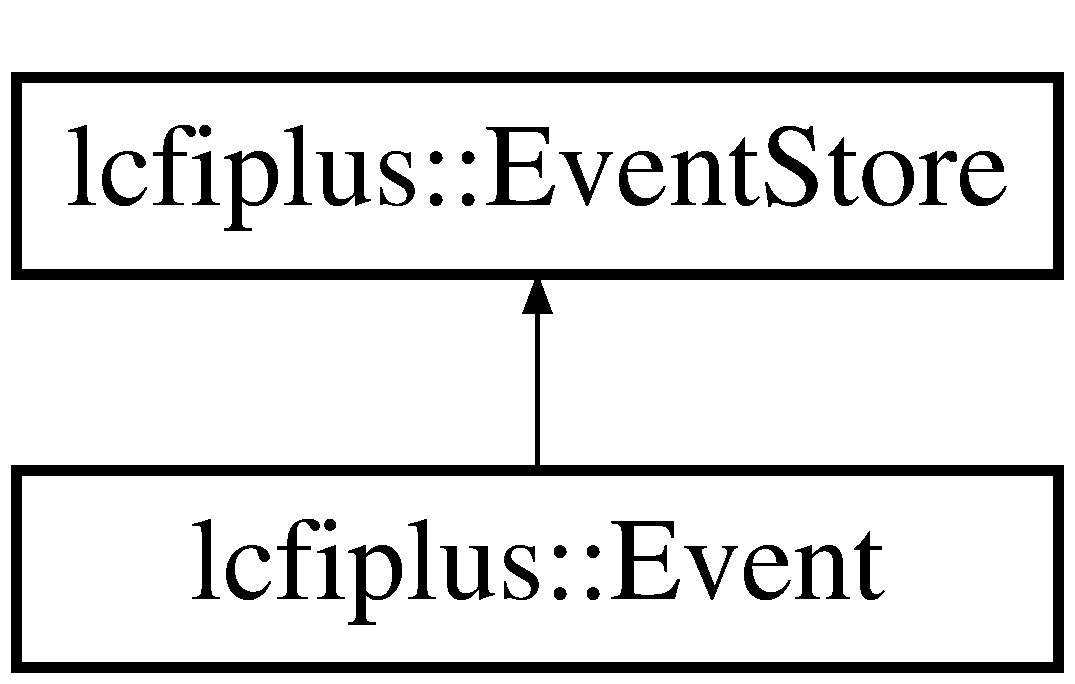
\includegraphics[height=2.000000cm]{classlcfiplus_1_1Event}
\end{center}
\end{figure}
\subsection*{Public Member Functions}
\begin{DoxyCompactItemize}
\item 
{\bf $\sim$\-Event} ()
\item 
const vector$<$ const {\bf Track} $\ast$ $>$ \& {\bf get\-Tracks} (const char $\ast$trackname=0) const 
\item 
const vector$<$ const {\bf Neutral} $\ast$ $>$ \& {\bf get\-Neutrals} (const char $\ast$neutralname=0) const 
\item 
const vector$<$ const {\bf M\-C\-Particle} $\ast$ $>$ \& {\bf get\-M\-C\-Particles} (const char $\ast$mcpname=0) const 
\item 
const vector$<$ const \\*
{\bf M\-C\-Color\-Singlet} $\ast$ $>$ \& {\bf get\-M\-C\-Color\-Singlets} (const char $\ast$mcpname=0) const 
\item 
const {\bf Vertex} $\ast$ {\bf get\-Primary\-Vertex} (const char $\ast$privtxname=0) const 
\item 
const vector$<$ const {\bf Vertex} $\ast$ $>$ \& {\bf get\-Secondary\-Vertices} (const char $\ast$secvtxname=0) const 
\item 
const vector$<$ const {\bf Jet} $\ast$ $>$ \& {\bf get\-Jets} (const char $\ast$jetname=0) const 
\item 
void {\bf set\-Default\-Tracks} (const char $\ast$name)
\item 
void {\bf set\-Default\-Neutrals} (const char $\ast$name)
\item 
void {\bf set\-Default\-M\-C\-Particles} (const char $\ast$name)
\item 
void {\bf set\-Default\-Primary\-Vertex} (const char $\ast$name)
\item 
void {\bf set\-Default\-Secondary\-Vertices} (const char $\ast$name)
\item 
void {\bf set\-Default\-Jets} (const char $\ast$name)
\item 
const char $\ast$ {\bf get\-Default\-Tracks} () const 
\item 
const char $\ast$ {\bf get\-Default\-Neutrals} () const 
\item 
const char $\ast$ {\bf get\-Default\-M\-C\-Particles} () const 
\item 
const char $\ast$ {\bf get\-Default\-Primary\-Vertex} () const 
\item 
const char $\ast$ {\bf get\-Default\-Secondary\-Vertices} () const 
\item 
const char $\ast$ {\bf get\-Default\-Jets} () const 
\item 
const {\bf M\-C\-Particle} $\ast$ {\bf get\-M\-C\-Particle} (int id) const 
\item 
const {\bf M\-C\-Particle} $\ast$ {\bf get\-M\-C\-Particle} (const {\bf Track} $\ast$trk) const 
\item 
vector$<$ const {\bf M\-C\-Particle} $\ast$ $>$ {\bf mc\-Get\-Color\-Strings} () const 
\item 
int {\bf mc\-Number\-Of\-B} () const 
\item 
int {\bf mc\-Number\-Of\-C} () const 
\item 
vector$<$ const {\bf M\-C\-Particle} $\ast$ $>$ {\bf mc\-Get\-Semi\-Stable\-Bs} () const 
\item 
vector$<$ const {\bf M\-C\-Particle} $\ast$ $>$ {\bf mc\-Get\-Semi\-Stable\-Cs} () const 
\item 
vector$<$ const {\bf M\-C\-Particle} $\ast$ $>$ {\bf mc\-Get\-Semi\-Stable\-B\-Cs} (bool separatebc) const 
\item 
int {\bf mc\-Find\-Parent} ({\bf M\-C\-Particle\-Vec} \&vec, const {\bf M\-C\-Particle} $\ast$p) const 
\end{DoxyCompactItemize}
\subsection*{Static Public Member Functions}
\begin{DoxyCompactItemize}
\item 
static {\bf Event} $\ast$ {\bf Instance} ()
\end{DoxyCompactItemize}
\subsection*{Additional Inherited Members}


\subsection{Constructor \& Destructor Documentation}
\index{lcfiplus\-::\-Event@{lcfiplus\-::\-Event}!$\sim$\-Event@{$\sim$\-Event}}
\index{$\sim$\-Event@{$\sim$\-Event}!lcfiplus::Event@{lcfiplus\-::\-Event}}
\subsubsection[{$\sim$\-Event}]{\setlength{\rightskip}{0pt plus 5cm}lcfiplus\-::\-Event\-::$\sim$\-Event (
\begin{DoxyParamCaption}
{}
\end{DoxyParamCaption}
)}\label{classlcfiplus_1_1Event_a947199c20186456a74bc387e0daa2ade}


\subsection{Member Function Documentation}
\index{lcfiplus\-::\-Event@{lcfiplus\-::\-Event}!get\-Default\-Jets@{get\-Default\-Jets}}
\index{get\-Default\-Jets@{get\-Default\-Jets}!lcfiplus::Event@{lcfiplus\-::\-Event}}
\subsubsection[{get\-Default\-Jets}]{\setlength{\rightskip}{0pt plus 5cm}const char$\ast$ lcfiplus\-::\-Event\-::get\-Default\-Jets (
\begin{DoxyParamCaption}
{}
\end{DoxyParamCaption}
) const\hspace{0.3cm}{\ttfamily [inline]}}\label{classlcfiplus_1_1Event_a2ad73a5bed0e52b248e54ad222d7c96f}
\index{lcfiplus\-::\-Event@{lcfiplus\-::\-Event}!get\-Default\-M\-C\-Particles@{get\-Default\-M\-C\-Particles}}
\index{get\-Default\-M\-C\-Particles@{get\-Default\-M\-C\-Particles}!lcfiplus::Event@{lcfiplus\-::\-Event}}
\subsubsection[{get\-Default\-M\-C\-Particles}]{\setlength{\rightskip}{0pt plus 5cm}const char$\ast$ lcfiplus\-::\-Event\-::get\-Default\-M\-C\-Particles (
\begin{DoxyParamCaption}
{}
\end{DoxyParamCaption}
) const\hspace{0.3cm}{\ttfamily [inline]}}\label{classlcfiplus_1_1Event_a7dcf5305cafee539a7f7f04998f0e29b}
\index{lcfiplus\-::\-Event@{lcfiplus\-::\-Event}!get\-Default\-Neutrals@{get\-Default\-Neutrals}}
\index{get\-Default\-Neutrals@{get\-Default\-Neutrals}!lcfiplus::Event@{lcfiplus\-::\-Event}}
\subsubsection[{get\-Default\-Neutrals}]{\setlength{\rightskip}{0pt plus 5cm}const char$\ast$ lcfiplus\-::\-Event\-::get\-Default\-Neutrals (
\begin{DoxyParamCaption}
{}
\end{DoxyParamCaption}
) const\hspace{0.3cm}{\ttfamily [inline]}}\label{classlcfiplus_1_1Event_adba3f65d18c705668b128adab542457a}
\index{lcfiplus\-::\-Event@{lcfiplus\-::\-Event}!get\-Default\-Primary\-Vertex@{get\-Default\-Primary\-Vertex}}
\index{get\-Default\-Primary\-Vertex@{get\-Default\-Primary\-Vertex}!lcfiplus::Event@{lcfiplus\-::\-Event}}
\subsubsection[{get\-Default\-Primary\-Vertex}]{\setlength{\rightskip}{0pt plus 5cm}const char$\ast$ lcfiplus\-::\-Event\-::get\-Default\-Primary\-Vertex (
\begin{DoxyParamCaption}
{}
\end{DoxyParamCaption}
) const\hspace{0.3cm}{\ttfamily [inline]}}\label{classlcfiplus_1_1Event_acd3bd2e2213910c8ca5bc4d4081eac55}
\index{lcfiplus\-::\-Event@{lcfiplus\-::\-Event}!get\-Default\-Secondary\-Vertices@{get\-Default\-Secondary\-Vertices}}
\index{get\-Default\-Secondary\-Vertices@{get\-Default\-Secondary\-Vertices}!lcfiplus::Event@{lcfiplus\-::\-Event}}
\subsubsection[{get\-Default\-Secondary\-Vertices}]{\setlength{\rightskip}{0pt plus 5cm}const char$\ast$ lcfiplus\-::\-Event\-::get\-Default\-Secondary\-Vertices (
\begin{DoxyParamCaption}
{}
\end{DoxyParamCaption}
) const\hspace{0.3cm}{\ttfamily [inline]}}\label{classlcfiplus_1_1Event_a7f471c3b2e60d6a26df77b994bb3b8ca}
\index{lcfiplus\-::\-Event@{lcfiplus\-::\-Event}!get\-Default\-Tracks@{get\-Default\-Tracks}}
\index{get\-Default\-Tracks@{get\-Default\-Tracks}!lcfiplus::Event@{lcfiplus\-::\-Event}}
\subsubsection[{get\-Default\-Tracks}]{\setlength{\rightskip}{0pt plus 5cm}const char$\ast$ lcfiplus\-::\-Event\-::get\-Default\-Tracks (
\begin{DoxyParamCaption}
{}
\end{DoxyParamCaption}
) const\hspace{0.3cm}{\ttfamily [inline]}}\label{classlcfiplus_1_1Event_a5a89b6ca95ad69eb54138ecd6b3b7bfd}
\index{lcfiplus\-::\-Event@{lcfiplus\-::\-Event}!get\-Jets@{get\-Jets}}
\index{get\-Jets@{get\-Jets}!lcfiplus::Event@{lcfiplus\-::\-Event}}
\subsubsection[{get\-Jets}]{\setlength{\rightskip}{0pt plus 5cm}const vector$<$ const {\bf Jet} $\ast$ $>$ \& lcfiplus\-::\-Event\-::get\-Jets (
\begin{DoxyParamCaption}
\item[{const char $\ast$}]{jetname = {\ttfamily 0}}
\end{DoxyParamCaption}
) const}\label{classlcfiplus_1_1Event_a9be30ef5201291a3e8bf004eaab9a2cb}


References lcfiplus\-::\-Event\-Store\-::\-Get\-Object\-Ref().

\index{lcfiplus\-::\-Event@{lcfiplus\-::\-Event}!get\-M\-C\-Color\-Singlets@{get\-M\-C\-Color\-Singlets}}
\index{get\-M\-C\-Color\-Singlets@{get\-M\-C\-Color\-Singlets}!lcfiplus::Event@{lcfiplus\-::\-Event}}
\subsubsection[{get\-M\-C\-Color\-Singlets}]{\setlength{\rightskip}{0pt plus 5cm}{\bf M\-C\-Color\-Singlet\-Vec} \& lcfiplus\-::\-Event\-::get\-M\-C\-Color\-Singlets (
\begin{DoxyParamCaption}
\item[{const char $\ast$}]{mcpname = {\ttfamily 0}}
\end{DoxyParamCaption}
) const}\label{classlcfiplus_1_1Event_a89884bd73a5b094a7b1a0379ad1461fb}


References lcfiplus\-::\-Event\-Store\-::\-Get\-Object\-Ref().

\index{lcfiplus\-::\-Event@{lcfiplus\-::\-Event}!get\-M\-C\-Particle@{get\-M\-C\-Particle}}
\index{get\-M\-C\-Particle@{get\-M\-C\-Particle}!lcfiplus::Event@{lcfiplus\-::\-Event}}
\subsubsection[{get\-M\-C\-Particle}]{\setlength{\rightskip}{0pt plus 5cm}const {\bf M\-C\-Particle} $\ast$ lcfiplus\-::\-Event\-::get\-M\-C\-Particle (
\begin{DoxyParamCaption}
\item[{int}]{id}
\end{DoxyParamCaption}
) const}\label{classlcfiplus_1_1Event_ad1d08ee041d71095863477ddd5d917f9}


References lcfiplus\-::\-M\-C\-Particle\-::get\-Id(), and get\-M\-C\-Particles().



Referenced by lcfiplus\-::find\-Tear\-Down\-Vertices(), and match\-Mc\-Vertex\-Jet().

\index{lcfiplus\-::\-Event@{lcfiplus\-::\-Event}!get\-M\-C\-Particle@{get\-M\-C\-Particle}}
\index{get\-M\-C\-Particle@{get\-M\-C\-Particle}!lcfiplus::Event@{lcfiplus\-::\-Event}}
\subsubsection[{get\-M\-C\-Particle}]{\setlength{\rightskip}{0pt plus 5cm}const {\bf M\-C\-Particle} $\ast$ lcfiplus\-::\-Event\-::get\-M\-C\-Particle (
\begin{DoxyParamCaption}
\item[{const {\bf Track} $\ast$}]{trk}
\end{DoxyParamCaption}
) const}\label{classlcfiplus_1_1Event_a458fe4c20acbdbe603965fb80a2665a9}


References lcfiplus\-::\-Track\-::get\-Mcp().

\index{lcfiplus\-::\-Event@{lcfiplus\-::\-Event}!get\-M\-C\-Particles@{get\-M\-C\-Particles}}
\index{get\-M\-C\-Particles@{get\-M\-C\-Particles}!lcfiplus::Event@{lcfiplus\-::\-Event}}
\subsubsection[{get\-M\-C\-Particles}]{\setlength{\rightskip}{0pt plus 5cm}{\bf M\-C\-Particle\-Vec} \& lcfiplus\-::\-Event\-::get\-M\-C\-Particles (
\begin{DoxyParamCaption}
\item[{const char $\ast$}]{mcpname = {\ttfamily 0}}
\end{DoxyParamCaption}
) const}\label{classlcfiplus_1_1Event_af8c15d57d1636b05a42834343c901ce4}


References lcfiplus\-::\-Event\-Store\-::\-Get\-Object\-Ref().



Referenced by get\-M\-C\-Particle(), mc\-Get\-Color\-Strings(), mc\-Get\-Semi\-Stable\-B\-Cs(), mc\-Get\-Semi\-Stable\-Bs(), mc\-Get\-Semi\-Stable\-Cs(), mc\-Number\-Of\-B(), mc\-Number\-Of\-C(), lcfiplus\-::\-Z\-H\-H\-Algo\-::process(), and lcfiplus\-::\-Vertex\-Analysis\-::process().

\index{lcfiplus\-::\-Event@{lcfiplus\-::\-Event}!get\-Neutrals@{get\-Neutrals}}
\index{get\-Neutrals@{get\-Neutrals}!lcfiplus::Event@{lcfiplus\-::\-Event}}
\subsubsection[{get\-Neutrals}]{\setlength{\rightskip}{0pt plus 5cm}{\bf Neutral\-Vec} \& lcfiplus\-::\-Event\-::get\-Neutrals (
\begin{DoxyParamCaption}
\item[{const char $\ast$}]{neutralname = {\ttfamily 0}}
\end{DoxyParamCaption}
) const}\label{classlcfiplus_1_1Event_a122c7c012ec139ced9c8c56a1143e4cd}


References lcfiplus\-::\-Event\-Store\-::\-Get\-Object\-Ref().



Referenced by match\-Mc\-Vertex\-Reco\-V0(), and lcfiplus\-::\-Z\-H\-H\-Algo\-::process().

\index{lcfiplus\-::\-Event@{lcfiplus\-::\-Event}!get\-Primary\-Vertex@{get\-Primary\-Vertex}}
\index{get\-Primary\-Vertex@{get\-Primary\-Vertex}!lcfiplus::Event@{lcfiplus\-::\-Event}}
\subsubsection[{get\-Primary\-Vertex}]{\setlength{\rightskip}{0pt plus 5cm}const {\bf Vertex} $\ast$ lcfiplus\-::\-Event\-::get\-Primary\-Vertex (
\begin{DoxyParamCaption}
\item[{const char $\ast$}]{privtxname = {\ttfamily 0}}
\end{DoxyParamCaption}
) const}\label{classlcfiplus_1_1Event_afadc0d3d6d5920781afc26edd7f6b462}


References lcfiplus\-::\-Event\-Store\-::\-Get\-Object().



Referenced by lcfiplus\-::\-Jet\-::get\-All\-Tracks(), lcfiplus\-::\-Z\-H\-H\-Algo\-::process(), lcfiplus\-::\-Test\-Algo\-::process(), and lcfiplus\-::\-Vertex\-Analysis\-::process().

\index{lcfiplus\-::\-Event@{lcfiplus\-::\-Event}!get\-Secondary\-Vertices@{get\-Secondary\-Vertices}}
\index{get\-Secondary\-Vertices@{get\-Secondary\-Vertices}!lcfiplus::Event@{lcfiplus\-::\-Event}}
\subsubsection[{get\-Secondary\-Vertices}]{\setlength{\rightskip}{0pt plus 5cm}const vector$<$ const {\bf Vertex} $\ast$ $>$ \& lcfiplus\-::\-Event\-::get\-Secondary\-Vertices (
\begin{DoxyParamCaption}
\item[{const char $\ast$}]{secvtxname = {\ttfamily 0}}
\end{DoxyParamCaption}
) const}\label{classlcfiplus_1_1Event_a4de957fd20d1cbb8c1b72d607e306179}


References lcfiplus\-::\-Event\-Store\-::\-Get\-Object\-Ref().

\index{lcfiplus\-::\-Event@{lcfiplus\-::\-Event}!get\-Tracks@{get\-Tracks}}
\index{get\-Tracks@{get\-Tracks}!lcfiplus::Event@{lcfiplus\-::\-Event}}
\subsubsection[{get\-Tracks}]{\setlength{\rightskip}{0pt plus 5cm}{\bf Track\-Vec} \& lcfiplus\-::\-Event\-::get\-Tracks (
\begin{DoxyParamCaption}
\item[{const char $\ast$}]{trackname = {\ttfamily 0}}
\end{DoxyParamCaption}
) const}\label{classlcfiplus_1_1Event_acec181fe87fbba13f19d97199c7e1ec1}


References lcfiplus\-::\-Event\-Store\-::\-Get\-Object\-Ref().



Referenced by lcfiplus\-::\-Jet\-M\-C\-Match(), match\-Mc\-Vertex(), match\-Mc\-Vertex\-Jet(), lcfiplus\-::\-Z\-H\-H\-Algo\-::process(), and lcfiplus\-::\-Vertex\-Analysis\-::process().

\index{lcfiplus\-::\-Event@{lcfiplus\-::\-Event}!Instance@{Instance}}
\index{Instance@{Instance}!lcfiplus::Event@{lcfiplus\-::\-Event}}
\subsubsection[{Instance}]{\setlength{\rightskip}{0pt plus 5cm}{\bf Event} $\ast$ lcfiplus\-::\-Event\-::\-Instance (
\begin{DoxyParamCaption}
{}
\end{DoxyParamCaption}
)\hspace{0.3cm}{\ttfamily [static]}}\label{classlcfiplus_1_1Event_a2b3279db0def68be064f2b7b6752b74b}


Referenced by lcfiplus\-::\-Event\-Navigator\-::\-Fwd(), lcfiplus\-::\-Jet\-::get\-All\-Tracks(), lcfiplus\-::\-Vertex\-Mass\-Recovery\-::init(), lcfiplus\-::\-Primary\-Vertex\-Finder\-::init(), lcfiplus\-::\-Vertex\-Ntuple\-::init(), lcfiplus\-::\-Track\-Ntuple\-::init(), lcfiplus\-::\-Flavor\-Tag\-::init(), lcfiplus\-::\-Build\-Up\-Vertex\-::init(), lcfiplus\-::\-Jet\-Clustering\-::init(), lcfiplus\-::\-Jet\-Vertex\-Refiner\-::init(), lcfiplus\-::\-Test\-Algo\-::init(), lcfiplus\-::\-Flavtag\-Reader\-::init(), lcfiplus\-::\-Jet\-M\-C\-Match(), lcfiplus\-::\-Vertex\-Mass\-Recovery\-::process(), lcfiplus\-::\-Primary\-Vertex\-Finder\-::process(), lcfiplus\-::\-Vertex\-Ntuple\-::process(), lcfiplus\-::\-Track\-Ntuple\-::process(), lcfiplus\-::\-Flavor\-Tag\-::process(), lcfiplus\-::\-Build\-Up\-Vertex\-::process(), lcfiplus\-::\-Jet\-Clustering\-::process(), lcfiplus\-::\-Jet\-Vertex\-Refiner\-::process(), lcfiplus\-::\-Z\-H\-H\-Algo\-::process(), lcfiplus\-::\-Test\-Algo\-::process(), lcfiplus\-::\-Vertex\-Analysis\-::process(), lcfiplus\-::\-Flavtag\-Reader\-::process(), lcfiplus\-::\-Test\-Algo\-V0\-::process(), lcfiplus\-::\-Tree\-Storer\-::\-Register(), test\-Suehara(), and test\-Tomohiko().

\index{lcfiplus\-::\-Event@{lcfiplus\-::\-Event}!mc\-Find\-Parent@{mc\-Find\-Parent}}
\index{mc\-Find\-Parent@{mc\-Find\-Parent}!lcfiplus::Event@{lcfiplus\-::\-Event}}
\subsubsection[{mc\-Find\-Parent}]{\setlength{\rightskip}{0pt plus 5cm}int lcfiplus\-::\-Event\-::mc\-Find\-Parent (
\begin{DoxyParamCaption}
\item[{{\bf M\-C\-Particle\-Vec} \&}]{vec, }
\item[{const {\bf M\-C\-Particle} $\ast$}]{p}
\end{DoxyParamCaption}
) const}\label{classlcfiplus_1_1Event_a4d737ed575e0dead7dd04981b84a5446}


References lcfiplus\-::\-M\-C\-Particle\-::is\-Parent().

\index{lcfiplus\-::\-Event@{lcfiplus\-::\-Event}!mc\-Get\-Color\-Strings@{mc\-Get\-Color\-Strings}}
\index{mc\-Get\-Color\-Strings@{mc\-Get\-Color\-Strings}!lcfiplus::Event@{lcfiplus\-::\-Event}}
\subsubsection[{mc\-Get\-Color\-Strings}]{\setlength{\rightskip}{0pt plus 5cm}vector$<$ const {\bf M\-C\-Particle} $\ast$ $>$ lcfiplus\-::\-Event\-::mc\-Get\-Color\-Strings (
\begin{DoxyParamCaption}
{}
\end{DoxyParamCaption}
) const}\label{classlcfiplus_1_1Event_a9c1925def78230d2cdafbb5e85dbcddb}


References lcfiplus\-::\-M\-C\-Particle\-::get\-Color\-String(), and get\-M\-C\-Particles().

\index{lcfiplus\-::\-Event@{lcfiplus\-::\-Event}!mc\-Get\-Semi\-Stable\-B\-Cs@{mc\-Get\-Semi\-Stable\-B\-Cs}}
\index{mc\-Get\-Semi\-Stable\-B\-Cs@{mc\-Get\-Semi\-Stable\-B\-Cs}!lcfiplus::Event@{lcfiplus\-::\-Event}}
\subsubsection[{mc\-Get\-Semi\-Stable\-B\-Cs}]{\setlength{\rightskip}{0pt plus 5cm}vector$<$ const {\bf M\-C\-Particle} $\ast$ $>$ lcfiplus\-::\-Event\-::mc\-Get\-Semi\-Stable\-B\-Cs (
\begin{DoxyParamCaption}
\item[{bool}]{separatebc}
\end{DoxyParamCaption}
) const}\label{classlcfiplus_1_1Event_a227173746c78c2f43e2a5e8a8c6c430f}


References get\-M\-C\-Particles(), lcfiplus\-::\-M\-C\-Particle\-::get\-Semi\-Stable\-B\-Parent(), and lcfiplus\-::\-M\-C\-Particle\-::get\-Semi\-Stable\-C\-Parent().

\index{lcfiplus\-::\-Event@{lcfiplus\-::\-Event}!mc\-Get\-Semi\-Stable\-Bs@{mc\-Get\-Semi\-Stable\-Bs}}
\index{mc\-Get\-Semi\-Stable\-Bs@{mc\-Get\-Semi\-Stable\-Bs}!lcfiplus::Event@{lcfiplus\-::\-Event}}
\subsubsection[{mc\-Get\-Semi\-Stable\-Bs}]{\setlength{\rightskip}{0pt plus 5cm}vector$<$ const {\bf M\-C\-Particle} $\ast$ $>$ lcfiplus\-::\-Event\-::mc\-Get\-Semi\-Stable\-Bs (
\begin{DoxyParamCaption}
{}
\end{DoxyParamCaption}
) const}\label{classlcfiplus_1_1Event_aff15a552e705199f53c7526d3e289f36}


References get\-M\-C\-Particles(), and lcfiplus\-::\-M\-C\-Particle\-::get\-Semi\-Stable\-B\-Parent().

\index{lcfiplus\-::\-Event@{lcfiplus\-::\-Event}!mc\-Get\-Semi\-Stable\-Cs@{mc\-Get\-Semi\-Stable\-Cs}}
\index{mc\-Get\-Semi\-Stable\-Cs@{mc\-Get\-Semi\-Stable\-Cs}!lcfiplus::Event@{lcfiplus\-::\-Event}}
\subsubsection[{mc\-Get\-Semi\-Stable\-Cs}]{\setlength{\rightskip}{0pt plus 5cm}vector$<$ const {\bf M\-C\-Particle} $\ast$ $>$ lcfiplus\-::\-Event\-::mc\-Get\-Semi\-Stable\-Cs (
\begin{DoxyParamCaption}
{}
\end{DoxyParamCaption}
) const}\label{classlcfiplus_1_1Event_ae981a54e5252a36aa9191d79e27cc43d}


References get\-M\-C\-Particles(), and lcfiplus\-::\-M\-C\-Particle\-::get\-Semi\-Stable\-C\-Parent().

\index{lcfiplus\-::\-Event@{lcfiplus\-::\-Event}!mc\-Number\-Of\-B@{mc\-Number\-Of\-B}}
\index{mc\-Number\-Of\-B@{mc\-Number\-Of\-B}!lcfiplus::Event@{lcfiplus\-::\-Event}}
\subsubsection[{mc\-Number\-Of\-B}]{\setlength{\rightskip}{0pt plus 5cm}int lcfiplus\-::\-Event\-::mc\-Number\-Of\-B (
\begin{DoxyParamCaption}
{}
\end{DoxyParamCaption}
) const}\label{classlcfiplus_1_1Event_aeccfeea9e62ee50255f33cfaee29f23c}


References get\-M\-C\-Particles(), and lcfiplus\-::\-M\-C\-Particle\-::is\-Semi\-Stable\-B().

\index{lcfiplus\-::\-Event@{lcfiplus\-::\-Event}!mc\-Number\-Of\-C@{mc\-Number\-Of\-C}}
\index{mc\-Number\-Of\-C@{mc\-Number\-Of\-C}!lcfiplus::Event@{lcfiplus\-::\-Event}}
\subsubsection[{mc\-Number\-Of\-C}]{\setlength{\rightskip}{0pt plus 5cm}int lcfiplus\-::\-Event\-::mc\-Number\-Of\-C (
\begin{DoxyParamCaption}
{}
\end{DoxyParamCaption}
) const}\label{classlcfiplus_1_1Event_ab0a8c503ea6cb7028dfee299de57a168}


References get\-M\-C\-Particles(), and lcfiplus\-::\-M\-C\-Particle\-::is\-Semi\-Stable\-C().

\index{lcfiplus\-::\-Event@{lcfiplus\-::\-Event}!set\-Default\-Jets@{set\-Default\-Jets}}
\index{set\-Default\-Jets@{set\-Default\-Jets}!lcfiplus::Event@{lcfiplus\-::\-Event}}
\subsubsection[{set\-Default\-Jets}]{\setlength{\rightskip}{0pt plus 5cm}void lcfiplus\-::\-Event\-::set\-Default\-Jets (
\begin{DoxyParamCaption}
\item[{const char $\ast$}]{name}
\end{DoxyParamCaption}
)\hspace{0.3cm}{\ttfamily [inline]}}\label{classlcfiplus_1_1Event_ab90cea4f3273359ffd244263fb760f71}
\index{lcfiplus\-::\-Event@{lcfiplus\-::\-Event}!set\-Default\-M\-C\-Particles@{set\-Default\-M\-C\-Particles}}
\index{set\-Default\-M\-C\-Particles@{set\-Default\-M\-C\-Particles}!lcfiplus::Event@{lcfiplus\-::\-Event}}
\subsubsection[{set\-Default\-M\-C\-Particles}]{\setlength{\rightskip}{0pt plus 5cm}void lcfiplus\-::\-Event\-::set\-Default\-M\-C\-Particles (
\begin{DoxyParamCaption}
\item[{const char $\ast$}]{name}
\end{DoxyParamCaption}
)\hspace{0.3cm}{\ttfamily [inline]}}\label{classlcfiplus_1_1Event_ada8f2072bbe3623b101f9727c0d0b771}
\index{lcfiplus\-::\-Event@{lcfiplus\-::\-Event}!set\-Default\-Neutrals@{set\-Default\-Neutrals}}
\index{set\-Default\-Neutrals@{set\-Default\-Neutrals}!lcfiplus::Event@{lcfiplus\-::\-Event}}
\subsubsection[{set\-Default\-Neutrals}]{\setlength{\rightskip}{0pt plus 5cm}void lcfiplus\-::\-Event\-::set\-Default\-Neutrals (
\begin{DoxyParamCaption}
\item[{const char $\ast$}]{name}
\end{DoxyParamCaption}
)\hspace{0.3cm}{\ttfamily [inline]}}\label{classlcfiplus_1_1Event_a80317cd29fa92ec7342615aee64f5cf6}
\index{lcfiplus\-::\-Event@{lcfiplus\-::\-Event}!set\-Default\-Primary\-Vertex@{set\-Default\-Primary\-Vertex}}
\index{set\-Default\-Primary\-Vertex@{set\-Default\-Primary\-Vertex}!lcfiplus::Event@{lcfiplus\-::\-Event}}
\subsubsection[{set\-Default\-Primary\-Vertex}]{\setlength{\rightskip}{0pt plus 5cm}void lcfiplus\-::\-Event\-::set\-Default\-Primary\-Vertex (
\begin{DoxyParamCaption}
\item[{const char $\ast$}]{name}
\end{DoxyParamCaption}
)\hspace{0.3cm}{\ttfamily [inline]}}\label{classlcfiplus_1_1Event_af7e191ebef047562f2b0c2f8bcefaf4e}


Referenced by lcfiplus\-::\-Primary\-Vertex\-Finder\-::init(), lcfiplus\-::\-Vertex\-Ntuple\-::init(), lcfiplus\-::\-Track\-Ntuple\-::init(), lcfiplus\-::\-Flavor\-Tag\-::init(), lcfiplus\-::\-Build\-Up\-Vertex\-::init(), lcfiplus\-::\-Test\-Algo\-::init(), and lcfiplus\-::\-Flavtag\-Reader\-::init().

\index{lcfiplus\-::\-Event@{lcfiplus\-::\-Event}!set\-Default\-Secondary\-Vertices@{set\-Default\-Secondary\-Vertices}}
\index{set\-Default\-Secondary\-Vertices@{set\-Default\-Secondary\-Vertices}!lcfiplus::Event@{lcfiplus\-::\-Event}}
\subsubsection[{set\-Default\-Secondary\-Vertices}]{\setlength{\rightskip}{0pt plus 5cm}void lcfiplus\-::\-Event\-::set\-Default\-Secondary\-Vertices (
\begin{DoxyParamCaption}
\item[{const char $\ast$}]{name}
\end{DoxyParamCaption}
)\hspace{0.3cm}{\ttfamily [inline]}}\label{classlcfiplus_1_1Event_a88a081cd465016e4f2f8102832ab10e9}


Referenced by lcfiplus\-::\-Test\-Algo\-::init().

\index{lcfiplus\-::\-Event@{lcfiplus\-::\-Event}!set\-Default\-Tracks@{set\-Default\-Tracks}}
\index{set\-Default\-Tracks@{set\-Default\-Tracks}!lcfiplus::Event@{lcfiplus\-::\-Event}}
\subsubsection[{set\-Default\-Tracks}]{\setlength{\rightskip}{0pt plus 5cm}void lcfiplus\-::\-Event\-::set\-Default\-Tracks (
\begin{DoxyParamCaption}
\item[{const char $\ast$}]{name}
\end{DoxyParamCaption}
)\hspace{0.3cm}{\ttfamily [inline]}}\label{classlcfiplus_1_1Event_a6124eb2d97edee392df2b2066be790dd}


The documentation for this class was generated from the following files\-:\begin{DoxyCompactItemize}
\item 
{\bf lcfiplus.\-h}\item 
{\bf lcfiplus.\-cc}\end{DoxyCompactItemize}

\section{lcfiplus\-:\-:Event\-Navigator Class Reference}
\label{classlcfiplus_1_1EventNavigator}\index{lcfiplus\-::\-Event\-Navigator@{lcfiplus\-::\-Event\-Navigator}}


\doxyref{Event}{p.}{classlcfiplus_1_1Event} display for L\-C\-F\-I\-Plus.  




{\ttfamily \#include $<$Event\-Navigator.\-h$>$}

\subsection*{Public Member Functions}
\begin{DoxyCompactItemize}
\item 
{\bf Event\-Navigator} (const char $\ast$input, int start=0)
\begin{DoxyCompactList}\small\item\em Constructor. \end{DoxyCompactList}\item 
{\bf $\sim$\-Event\-Navigator} ()
\item 
void {\bf Fwd} ()
\begin{DoxyCompactList}\small\item\em Display next event. \end{DoxyCompactList}\item 
void {\bf Bck} ()
\item 
void {\bf draw\-Event} ({\bf Event} $\ast$event)
\begin{DoxyCompactList}\small\item\em Draws given event. \end{DoxyCompactList}\end{DoxyCompactItemize}


\subsection{Detailed Description}
\doxyref{Event}{p.}{classlcfiplus_1_1Event} display for L\-C\-F\-I\-Plus. 

The graphics is based on the T\-Eve framework for R\-O\-O\-T. Adapted from the $<$a href="{\tt http\-://llr.\-in2p3.\-fr/$\sim$ruan/\-I\-L\-D\-Display/}$>$Druid event display.

\begin{DoxyAuthor}{Author}
T. Tanabe, I\-C\-E\-P\-P, The University of Tokyo 
\end{DoxyAuthor}
\begin{DoxyVersion}{Version}
\$\-Id\$ 
\end{DoxyVersion}


\subsection{Constructor \& Destructor Documentation}
\index{lcfiplus\-::\-Event\-Navigator@{lcfiplus\-::\-Event\-Navigator}!Event\-Navigator@{Event\-Navigator}}
\index{Event\-Navigator@{Event\-Navigator}!lcfiplus::EventNavigator@{lcfiplus\-::\-Event\-Navigator}}
\subsubsection[{Event\-Navigator}]{\setlength{\rightskip}{0pt plus 5cm}lcfiplus\-::\-Event\-Navigator\-::\-Event\-Navigator (
\begin{DoxyParamCaption}
\item[{const char $\ast$}]{input, }
\item[{int}]{start = {\ttfamily 0}}
\end{DoxyParamCaption}
)}\label{classlcfiplus_1_1EventNavigator_a6ee61abd6eb6ac9265d1ccb132d91510}


Constructor. 


\begin{DoxyParams}[1]{Parameters}
\mbox{\tt in}  & {\em input} & input file which contains events to inspect. \\
\hline
\mbox{\tt in}  & {\em start} & skips given number of events. \\
\hline
\end{DoxyParams}


References lcfiplus\-::\-L\-C\-I\-O\-Storer\-::\-Next().

\index{lcfiplus\-::\-Event\-Navigator@{lcfiplus\-::\-Event\-Navigator}!$\sim$\-Event\-Navigator@{$\sim$\-Event\-Navigator}}
\index{$\sim$\-Event\-Navigator@{$\sim$\-Event\-Navigator}!lcfiplus::EventNavigator@{lcfiplus\-::\-Event\-Navigator}}
\subsubsection[{$\sim$\-Event\-Navigator}]{\setlength{\rightskip}{0pt plus 5cm}lcfiplus\-::\-Event\-Navigator\-::$\sim$\-Event\-Navigator (
\begin{DoxyParamCaption}
{}
\end{DoxyParamCaption}
)}\label{classlcfiplus_1_1EventNavigator_ab0e80957435833bbcf04c4d11cf9de2f}


\subsection{Member Function Documentation}
\index{lcfiplus\-::\-Event\-Navigator@{lcfiplus\-::\-Event\-Navigator}!Bck@{Bck}}
\index{Bck@{Bck}!lcfiplus::EventNavigator@{lcfiplus\-::\-Event\-Navigator}}
\subsubsection[{Bck}]{\setlength{\rightskip}{0pt plus 5cm}void lcfiplus\-::\-Event\-Navigator\-::\-Bck (
\begin{DoxyParamCaption}
{}
\end{DoxyParamCaption}
)}\label{classlcfiplus_1_1EventNavigator_add85c2e4134c32f9c084dfc50715124b}
\index{lcfiplus\-::\-Event\-Navigator@{lcfiplus\-::\-Event\-Navigator}!draw\-Event@{draw\-Event}}
\index{draw\-Event@{draw\-Event}!lcfiplus::EventNavigator@{lcfiplus\-::\-Event\-Navigator}}
\subsubsection[{draw\-Event}]{\setlength{\rightskip}{0pt plus 5cm}void lcfiplus\-::\-Event\-Navigator\-::draw\-Event (
\begin{DoxyParamCaption}
\item[{{\bf Event} $\ast$}]{event}
\end{DoxyParamCaption}
)}\label{classlcfiplus_1_1EventNavigator_abfade858f734595fc0133ed1c869f6a8}


Draws given event. 



References lcfiplus\-::tpar\-::d0, lcfiplus\-::\-Globals\-::get\-B\-Field(), lcfiplus\-::\-Track\-::get\-Charge(), lcfiplus\-::\-M\-C\-Particle\-::get\-Charge(), lcfiplus\-::\-Vertex\-::get\-Chi2(), lcfiplus\-::\-Track\-::get\-D0(), lcfiplus\-::\-M\-C\-Particle\-::get\-Ex(), lcfiplus\-::\-M\-C\-Particle\-::get\-Ey(), lcfiplus\-::\-M\-C\-Particle\-::get\-Ez(), lcfiplus\-::\-M\-C\-Particle\-::get\-Flavor\-Tag\-Category(), lcfiplus\-::\-Track\-::get\-P\-D\-G(), lcfiplus\-::\-M\-C\-Particle\-::get\-P\-D\-G(), lcfiplus\-::\-Track\-::get\-Phi(), lcfiplus\-::\-Vertex\-::get\-Tracks(), lcfiplus\-::\-M\-C\-Particle\-::get\-Vertex(), lcfiplus\-::\-Vertex\-::get\-X(), lcfiplus\-::\-Vertex\-::get\-Y(), lcfiplus\-::\-Vertex\-::get\-Z(), lcfiplus\-::\-Track\-::get\-Z0(), lcfiplus\-::\-Globals\-::\-Instance(), lcfiplus\-::\-M\-C\-Particle\-::is\-Stable\-Track(), and lcfiplus\-::tpar\-::z0.



Referenced by Fwd().

\index{lcfiplus\-::\-Event\-Navigator@{lcfiplus\-::\-Event\-Navigator}!Fwd@{Fwd}}
\index{Fwd@{Fwd}!lcfiplus::EventNavigator@{lcfiplus\-::\-Event\-Navigator}}
\subsubsection[{Fwd}]{\setlength{\rightskip}{0pt plus 5cm}void lcfiplus\-::\-Event\-Navigator\-::\-Fwd (
\begin{DoxyParamCaption}
{}
\end{DoxyParamCaption}
)}\label{classlcfiplus_1_1EventNavigator_a2649c62f002c5e662496fb28785bb688}


Display next event. 



References draw\-Event(), lcfiplus\-::\-Event\-::\-Instance(), and lcfiplus\-::\-L\-C\-I\-O\-Storer\-::\-Next().



The documentation for this class was generated from the following files\-:\begin{DoxyCompactItemize}
\item 
{\bf Event\-Navigator.\-h}\item 
{\bf Event\-Navigator.\-cc}\end{DoxyCompactItemize}

\section{lcfiplus\-:\-:Event\-Store Class Reference}
\label{classlcfiplus_1_1EventStore}\index{lcfiplus\-::\-Event\-Store@{lcfiplus\-::\-Event\-Store}}


A simple named storage for event data.  




{\ttfamily \#include $<$Event\-Store.\-h$>$}

Inheritance diagram for lcfiplus\-:\-:Event\-Store\-:\begin{figure}[H]
\begin{center}
\leavevmode
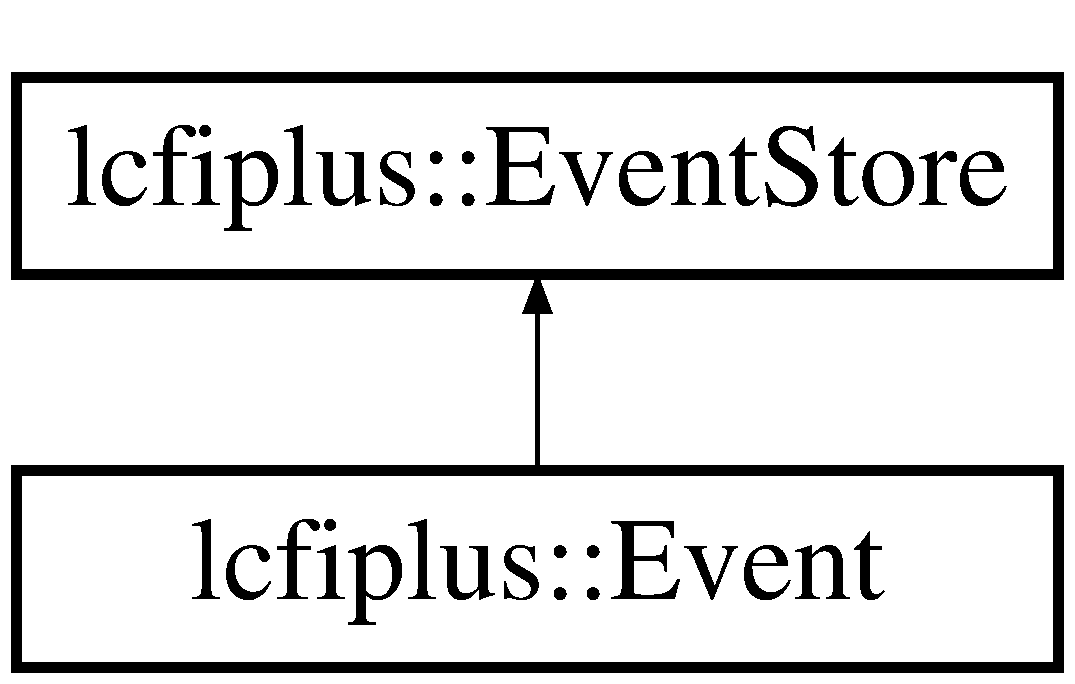
\includegraphics[height=2.000000cm]{classlcfiplus_1_1EventStore}
\end{center}
\end{figure}
\subsection*{Classes}
\begin{DoxyCompactItemize}
\item 
struct {\bf Stored\-Entry}
\end{DoxyCompactItemize}
\subsection*{Public Types}
\begin{DoxyCompactItemize}
\item 
enum \{ {\bf D\-O\-\_\-\-N\-O\-T\-\_\-\-D\-E\-L\-E\-T\-E} = 0x0001, 
{\bf P\-E\-R\-S\-I\-S\-T} = 0x0002, 
{\bf J\-E\-T\-\_\-\-W\-R\-I\-T\-E\-\_\-\-V\-E\-R\-T\-E\-X} = 0x1000
 \}
\end{DoxyCompactItemize}
\subsection*{Public Member Functions}
\begin{DoxyCompactItemize}
\item 
void {\bf Register\-Observer} ({\bf Event\-Store\-Observer} $\ast$observer)
\item 
void {\bf Unregister\-Observer} ({\bf Event\-Store\-Observer} $\ast$observer)
\item 
int {\bf Count} (const char $\ast$name) const 
\item 
bool {\bf Is\-Exist} (const char $\ast$name) const 
\item 
bool {\bf Is\-Exist} (const char $\ast$name, const char $\ast$classname) const 
\item 
const char $\ast$ {\bf Get\-Class\-Name} (const char $\ast$name, int idx=0) const 
\item 
void $\ast$ {\bf Get\-Object} (const char $\ast$name, const char $\ast$classname=\char`\"{}\char`\"{}) const 
\item 
{\footnotesize template$<$typename T $>$ }\\bool {\bf Get} (const char $\ast$name, const vector$<$ const T $\ast$ $>$ $\ast$\&buf) const 
\item 
{\footnotesize template$<$typename T $>$ }\\bool {\bf Get} (const char $\ast$name, const vector$<$ T $\ast$ $>$ $\ast$\&buf) const 
\item 
{\footnotesize template$<$typename T $>$ }\\bool {\bf Get} (const char $\ast$name, const vector$<$ T $>$ $\ast$\&buf) const 
\item 
{\footnotesize template$<$typename T $>$ }\\bool {\bf Get} (const char $\ast$name, const T $\ast$\&buf) const 
\item 
void $\ast$ {\bf Register\-Object} (const char $\ast$name, const char $\ast$classname, int flags=0)
\item 
{\footnotesize template$<$typename T $>$ }\\bool {\bf Register} (const char $\ast$name, vector$<$ T $\ast$ $>$ $\ast$\&buf, int flags=0)
\item 
{\footnotesize template$<$typename T $>$ }\\bool {\bf Register} (const char $\ast$name, vector$<$ T $>$ $\ast$\&buf, int flags=0)
\item 
{\footnotesize template$<$typename T $>$ }\\bool {\bf Register} (const char $\ast$name, T $\ast$\&buf, int flags=0)
\item 
void {\bf Print} () const 
\item 
void {\bf Clear\-Objects} ()
\item 
virtual {\bf $\sim$\-Event\-Store} ()
\item 
const multimap$<$ string, \\*
{\bf lcfiplus\-::\-Event\-Store\-::\-Stored\-Entry} $>$ \& {\bf Get\-Object\-Map} () const 
\end{DoxyCompactItemize}
\subsection*{Protected Member Functions}
\begin{DoxyCompactItemize}
\item 
void $\ast$const \& {\bf Get\-Object\-Ref} (const char $\ast$name, const char $\ast$classname=\char`\"{}\char`\"{}) const 
\item 
{\bf Event\-Store} ()
\end{DoxyCompactItemize}


\subsection{Detailed Description}
A simple named storage for event data. 

To obtain data\-: use Get(name) (in compiled code) or Get\-Object(name) (in C\-I\-N\-T)

C\-A\-U\-T\-I\-O\-N\-: \doxyref{Get\-Object()}{p.}{classlcfiplus_1_1EventStore_aef55ef7cd42d132a24d3a9bb629d9073} does not have type-\/check.

To register data\-: use Register(name) or Register\-Object(name, class) Use a pointer returned (cannot register a pointer from the caller). Any classes or vector of classes with Class\-Def() can be registered.

\begin{DoxyAuthor}{Author}
T. Suehara, I\-C\-E\-P\-P, The University of Tokyo 
\end{DoxyAuthor}
\begin{DoxyVersion}{Version}
\$\-Id\$ 
\end{DoxyVersion}


\subsection{Member Enumeration Documentation}
\subsubsection[{anonymous enum}]{\setlength{\rightskip}{0pt plus 5cm}anonymous enum}\label{classlcfiplus_1_1EventStore_a6b971b335bce75d19579cf0d9313878f}
\begin{Desc}
\item[Enumerator]\par
\begin{description}
\index{D\-O\-\_\-\-N\-O\-T\-\_\-\-D\-E\-L\-E\-T\-E@{D\-O\-\_\-\-N\-O\-T\-\_\-\-D\-E\-L\-E\-T\-E}!lcfiplus\-::\-Event\-Store@{lcfiplus\-::\-Event\-Store}}\index{lcfiplus\-::\-Event\-Store@{lcfiplus\-::\-Event\-Store}!D\-O\-\_\-\-N\-O\-T\-\_\-\-D\-E\-L\-E\-T\-E@{D\-O\-\_\-\-N\-O\-T\-\_\-\-D\-E\-L\-E\-T\-E}}\item[{\em 
D\-O\-\_\-\-N\-O\-T\-\_\-\-D\-E\-L\-E\-T\-E\label{classlcfiplus_1_1EventStore_a6b971b335bce75d19579cf0d9313878fa081715e1747df1fe9c75a320803c5ee1}
}]\index{P\-E\-R\-S\-I\-S\-T@{P\-E\-R\-S\-I\-S\-T}!lcfiplus\-::\-Event\-Store@{lcfiplus\-::\-Event\-Store}}\index{lcfiplus\-::\-Event\-Store@{lcfiplus\-::\-Event\-Store}!P\-E\-R\-S\-I\-S\-T@{P\-E\-R\-S\-I\-S\-T}}\item[{\em 
P\-E\-R\-S\-I\-S\-T\label{classlcfiplus_1_1EventStore_a6b971b335bce75d19579cf0d9313878faae90e2741e7e6e6687814bc34540d695}
}]\index{J\-E\-T\-\_\-\-W\-R\-I\-T\-E\-\_\-\-V\-E\-R\-T\-E\-X@{J\-E\-T\-\_\-\-W\-R\-I\-T\-E\-\_\-\-V\-E\-R\-T\-E\-X}!lcfiplus\-::\-Event\-Store@{lcfiplus\-::\-Event\-Store}}\index{lcfiplus\-::\-Event\-Store@{lcfiplus\-::\-Event\-Store}!J\-E\-T\-\_\-\-W\-R\-I\-T\-E\-\_\-\-V\-E\-R\-T\-E\-X@{J\-E\-T\-\_\-\-W\-R\-I\-T\-E\-\_\-\-V\-E\-R\-T\-E\-X}}\item[{\em 
J\-E\-T\-\_\-\-W\-R\-I\-T\-E\-\_\-\-V\-E\-R\-T\-E\-X\label{classlcfiplus_1_1EventStore_a6b971b335bce75d19579cf0d9313878fab41d7f557575ae7c97207f74cd727c29}
}]\end{description}
\end{Desc}


\subsection{Constructor \& Destructor Documentation}
\index{lcfiplus\-::\-Event\-Store@{lcfiplus\-::\-Event\-Store}!$\sim$\-Event\-Store@{$\sim$\-Event\-Store}}
\index{$\sim$\-Event\-Store@{$\sim$\-Event\-Store}!lcfiplus::EventStore@{lcfiplus\-::\-Event\-Store}}
\subsubsection[{$\sim$\-Event\-Store}]{\setlength{\rightskip}{0pt plus 5cm}lcfiplus\-::\-Event\-Store\-::$\sim$\-Event\-Store (
\begin{DoxyParamCaption}
{}
\end{DoxyParamCaption}
)\hspace{0.3cm}{\ttfamily [virtual]}}\label{classlcfiplus_1_1EventStore_adb15eb43c0a69bf92bfd5ac414d4c2f4}
\index{lcfiplus\-::\-Event\-Store@{lcfiplus\-::\-Event\-Store}!Event\-Store@{Event\-Store}}
\index{Event\-Store@{Event\-Store}!lcfiplus::EventStore@{lcfiplus\-::\-Event\-Store}}
\subsubsection[{Event\-Store}]{\setlength{\rightskip}{0pt plus 5cm}lcfiplus\-::\-Event\-Store\-::\-Event\-Store (
\begin{DoxyParamCaption}
{}
\end{DoxyParamCaption}
)\hspace{0.3cm}{\ttfamily [protected]}}\label{classlcfiplus_1_1EventStore_a221074c0fc374a7165cf2b627b03c897}


\subsection{Member Function Documentation}
\index{lcfiplus\-::\-Event\-Store@{lcfiplus\-::\-Event\-Store}!Clear\-Objects@{Clear\-Objects}}
\index{Clear\-Objects@{Clear\-Objects}!lcfiplus::EventStore@{lcfiplus\-::\-Event\-Store}}
\subsubsection[{Clear\-Objects}]{\setlength{\rightskip}{0pt plus 5cm}void lcfiplus\-::\-Event\-Store\-::\-Clear\-Objects (
\begin{DoxyParamCaption}
{}
\end{DoxyParamCaption}
)}\label{classlcfiplus_1_1EventStore_a1a72eb2332cf2f7c763f484213e29a15}


References lcfiplus\-::\-Event\-Store\-::\-Stored\-Entry\-::classname, lcfiplus\-::\-Event\-Store\-::\-Stored\-Entry\-::flag, and lcfiplus\-::\-Event\-Store\-::\-Stored\-Entry\-::obj.

\index{lcfiplus\-::\-Event\-Store@{lcfiplus\-::\-Event\-Store}!Count@{Count}}
\index{Count@{Count}!lcfiplus::EventStore@{lcfiplus\-::\-Event\-Store}}
\subsubsection[{Count}]{\setlength{\rightskip}{0pt plus 5cm}int lcfiplus\-::\-Event\-Store\-::\-Count (
\begin{DoxyParamCaption}
\item[{const char $\ast$}]{name}
\end{DoxyParamCaption}
) const}\label{classlcfiplus_1_1EventStore_ae242395d11cd5d63698be79cecaefa6b}
\index{lcfiplus\-::\-Event\-Store@{lcfiplus\-::\-Event\-Store}!Get@{Get}}
\index{Get@{Get}!lcfiplus::EventStore@{lcfiplus\-::\-Event\-Store}}
\subsubsection[{Get}]{\setlength{\rightskip}{0pt plus 5cm}template$<$typename T $>$ bool lcfiplus\-::\-Event\-Store\-::\-Get (
\begin{DoxyParamCaption}
\item[{const char $\ast$}]{name, }
\item[{const vector$<$ const T $\ast$ $>$ $\ast$\&}]{buf}
\end{DoxyParamCaption}
) const}\label{classlcfiplus_1_1EventStore_af7a38a2524940baade9f9c52f08a4d13}


Referenced by lcfiplus\-::\-Jet\-Clustering\-::init(), lcfiplus\-::\-Build\-Up\-Vertex\-::process(), lcfiplus\-::\-Jet\-Clustering\-::process(), lcfiplus\-::\-Z\-H\-H\-Algo\-::process(), lcfiplus\-::\-Test\-Algo\-::process(), lcfiplus\-::\-Vertex\-Analysis\-::process(), lcfiplus\-::\-Flavtag\-Reader\-::process(), and lcfiplus\-::\-Test\-Algo\-V0\-::process().

\index{lcfiplus\-::\-Event\-Store@{lcfiplus\-::\-Event\-Store}!Get@{Get}}
\index{Get@{Get}!lcfiplus::EventStore@{lcfiplus\-::\-Event\-Store}}
\subsubsection[{Get}]{\setlength{\rightskip}{0pt plus 5cm}template$<$typename T $>$ bool lcfiplus\-::\-Event\-Store\-::\-Get (
\begin{DoxyParamCaption}
\item[{const char $\ast$}]{name, }
\item[{const vector$<$ T $\ast$ $>$ $\ast$\&}]{buf}
\end{DoxyParamCaption}
) const}\label{classlcfiplus_1_1EventStore_a7edbe7e4ae89ab8529f383a6b5dd3101}
\index{lcfiplus\-::\-Event\-Store@{lcfiplus\-::\-Event\-Store}!Get@{Get}}
\index{Get@{Get}!lcfiplus::EventStore@{lcfiplus\-::\-Event\-Store}}
\subsubsection[{Get}]{\setlength{\rightskip}{0pt plus 5cm}template$<$typename T $>$ bool lcfiplus\-::\-Event\-Store\-::\-Get (
\begin{DoxyParamCaption}
\item[{const char $\ast$}]{name, }
\item[{const vector$<$ T $>$ $\ast$\&}]{buf}
\end{DoxyParamCaption}
) const}\label{classlcfiplus_1_1EventStore_a6d40448a9fcd5c4e239f4cd70607dd92}
\index{lcfiplus\-::\-Event\-Store@{lcfiplus\-::\-Event\-Store}!Get@{Get}}
\index{Get@{Get}!lcfiplus::EventStore@{lcfiplus\-::\-Event\-Store}}
\subsubsection[{Get}]{\setlength{\rightskip}{0pt plus 5cm}template$<$typename T $>$ bool lcfiplus\-::\-Event\-Store\-::\-Get (
\begin{DoxyParamCaption}
\item[{const char $\ast$}]{name, }
\item[{const T $\ast$\&}]{buf}
\end{DoxyParamCaption}
) const}\label{classlcfiplus_1_1EventStore_a8101e4d1c2e55878c9fa715cc1b445a0}
\index{lcfiplus\-::\-Event\-Store@{lcfiplus\-::\-Event\-Store}!Get\-Class\-Name@{Get\-Class\-Name}}
\index{Get\-Class\-Name@{Get\-Class\-Name}!lcfiplus::EventStore@{lcfiplus\-::\-Event\-Store}}
\subsubsection[{Get\-Class\-Name}]{\setlength{\rightskip}{0pt plus 5cm}const char $\ast$ lcfiplus\-::\-Event\-Store\-::\-Get\-Class\-Name (
\begin{DoxyParamCaption}
\item[{const char $\ast$}]{name, }
\item[{int}]{idx = {\ttfamily 0}}
\end{DoxyParamCaption}
) const}\label{classlcfiplus_1_1EventStore_aac51574826b1bb67b2cbd39fda9865ca}


Referenced by lcfiplus\-::\-Tree\-Storer\-::\-Register().

\index{lcfiplus\-::\-Event\-Store@{lcfiplus\-::\-Event\-Store}!Get\-Object@{Get\-Object}}
\index{Get\-Object@{Get\-Object}!lcfiplus::EventStore@{lcfiplus\-::\-Event\-Store}}
\subsubsection[{Get\-Object}]{\setlength{\rightskip}{0pt plus 5cm}void $\ast$ lcfiplus\-::\-Event\-Store\-::\-Get\-Object (
\begin{DoxyParamCaption}
\item[{const char $\ast$}]{name, }
\item[{const char $\ast$}]{classname = {\ttfamily \char`\"{}\char`\"{}}}
\end{DoxyParamCaption}
) const}\label{classlcfiplus_1_1EventStore_aef55ef7cd42d132a24d3a9bb629d9073}


Referenced by lcfiplus\-::\-Event\-::get\-Primary\-Vertex(), and lcfiplus\-::\-Tree\-Storer\-::\-Register().

\index{lcfiplus\-::\-Event\-Store@{lcfiplus\-::\-Event\-Store}!Get\-Object\-Map@{Get\-Object\-Map}}
\index{Get\-Object\-Map@{Get\-Object\-Map}!lcfiplus::EventStore@{lcfiplus\-::\-Event\-Store}}
\subsubsection[{Get\-Object\-Map}]{\setlength{\rightskip}{0pt plus 5cm}const multimap$<$string, {\bf lcfiplus\-::\-Event\-Store\-::\-Stored\-Entry} $>$\& lcfiplus\-::\-Event\-Store\-::\-Get\-Object\-Map (
\begin{DoxyParamCaption}
{}
\end{DoxyParamCaption}
) const\hspace{0.3cm}{\ttfamily [inline]}}\label{classlcfiplus_1_1EventStore_a507d840435cd6866ae4ce6cb6c57995a}


Referenced by lcfiplus\-::\-L\-C\-I\-O\-Storer\-::\-Auto\-Convert().

\index{lcfiplus\-::\-Event\-Store@{lcfiplus\-::\-Event\-Store}!Get\-Object\-Ref@{Get\-Object\-Ref}}
\index{Get\-Object\-Ref@{Get\-Object\-Ref}!lcfiplus::EventStore@{lcfiplus\-::\-Event\-Store}}
\subsubsection[{Get\-Object\-Ref}]{\setlength{\rightskip}{0pt plus 5cm}void $\ast$const \& lcfiplus\-::\-Event\-Store\-::\-Get\-Object\-Ref (
\begin{DoxyParamCaption}
\item[{const char $\ast$}]{name, }
\item[{const char $\ast$}]{classname = {\ttfamily \char`\"{}\char`\"{}}}
\end{DoxyParamCaption}
) const\hspace{0.3cm}{\ttfamily [protected]}}\label{classlcfiplus_1_1EventStore_a6640169c3eab5f9339272f6df9f5872f}


Referenced by lcfiplus\-::\-Event\-::get\-Jets(), lcfiplus\-::\-Event\-::get\-M\-C\-Color\-Singlets(), lcfiplus\-::\-Event\-::get\-M\-C\-Particles(), lcfiplus\-::\-Event\-::get\-Neutrals(), lcfiplus\-::\-Event\-::get\-Secondary\-Vertices(), and lcfiplus\-::\-Event\-::get\-Tracks().

\index{lcfiplus\-::\-Event\-Store@{lcfiplus\-::\-Event\-Store}!Is\-Exist@{Is\-Exist}}
\index{Is\-Exist@{Is\-Exist}!lcfiplus::EventStore@{lcfiplus\-::\-Event\-Store}}
\subsubsection[{Is\-Exist}]{\setlength{\rightskip}{0pt plus 5cm}bool lcfiplus\-::\-Event\-Store\-::\-Is\-Exist (
\begin{DoxyParamCaption}
\item[{const char $\ast$}]{name}
\end{DoxyParamCaption}
) const\hspace{0.3cm}{\ttfamily [inline]}}\label{classlcfiplus_1_1EventStore_a3858f2163cea6491888d89f339fc3dba}
\index{lcfiplus\-::\-Event\-Store@{lcfiplus\-::\-Event\-Store}!Is\-Exist@{Is\-Exist}}
\index{Is\-Exist@{Is\-Exist}!lcfiplus::EventStore@{lcfiplus\-::\-Event\-Store}}
\subsubsection[{Is\-Exist}]{\setlength{\rightskip}{0pt plus 5cm}bool lcfiplus\-::\-Event\-Store\-::\-Is\-Exist (
\begin{DoxyParamCaption}
\item[{const char $\ast$}]{name, }
\item[{const char $\ast$}]{classname}
\end{DoxyParamCaption}
) const}\label{classlcfiplus_1_1EventStore_ad7ef3c4f4da14808b60b14e4f62349bd}
\index{lcfiplus\-::\-Event\-Store@{lcfiplus\-::\-Event\-Store}!Print@{Print}}
\index{Print@{Print}!lcfiplus::EventStore@{lcfiplus\-::\-Event\-Store}}
\subsubsection[{Print}]{\setlength{\rightskip}{0pt plus 5cm}void lcfiplus\-::\-Event\-Store\-::\-Print (
\begin{DoxyParamCaption}
{}
\end{DoxyParamCaption}
) const}\label{classlcfiplus_1_1EventStore_adfd175639e8ced4372c08daa7d5f6e6e}
\index{lcfiplus\-::\-Event\-Store@{lcfiplus\-::\-Event\-Store}!Register@{Register}}
\index{Register@{Register}!lcfiplus::EventStore@{lcfiplus\-::\-Event\-Store}}
\subsubsection[{Register}]{\setlength{\rightskip}{0pt plus 5cm}template$<$typename T $>$ bool lcfiplus\-::\-Event\-Store\-::\-Register (
\begin{DoxyParamCaption}
\item[{const char $\ast$}]{name, }
\item[{vector$<$ T $\ast$ $>$ $\ast$\&}]{buf, }
\item[{int}]{flags = {\ttfamily 0}}
\end{DoxyParamCaption}
)}\label{classlcfiplus_1_1EventStore_a7dd922802076dea2440dcc65720a83ad}


Referenced by lcfiplus\-::\-Vertex\-Mass\-Recovery\-::init(), lcfiplus\-::\-Primary\-Vertex\-Finder\-::init(), lcfiplus\-::\-Build\-Up\-Vertex\-::init(), lcfiplus\-::\-Jet\-Clustering\-::init(), and lcfiplus\-::\-Jet\-Vertex\-Refiner\-::init().

\index{lcfiplus\-::\-Event\-Store@{lcfiplus\-::\-Event\-Store}!Register@{Register}}
\index{Register@{Register}!lcfiplus::EventStore@{lcfiplus\-::\-Event\-Store}}
\subsubsection[{Register}]{\setlength{\rightskip}{0pt plus 5cm}template$<$typename T $>$ bool lcfiplus\-::\-Event\-Store\-::\-Register (
\begin{DoxyParamCaption}
\item[{const char $\ast$}]{name, }
\item[{vector$<$ T $>$ $\ast$\&}]{buf, }
\item[{int}]{flags = {\ttfamily 0}}
\end{DoxyParamCaption}
)}\label{classlcfiplus_1_1EventStore_a9eef473240c352825b5922e754910549}
\index{lcfiplus\-::\-Event\-Store@{lcfiplus\-::\-Event\-Store}!Register@{Register}}
\index{Register@{Register}!lcfiplus::EventStore@{lcfiplus\-::\-Event\-Store}}
\subsubsection[{Register}]{\setlength{\rightskip}{0pt plus 5cm}template$<$typename T $>$ bool lcfiplus\-::\-Event\-Store\-::\-Register (
\begin{DoxyParamCaption}
\item[{const char $\ast$}]{name, }
\item[{T $\ast$\&}]{buf, }
\item[{int}]{flags = {\ttfamily 0}}
\end{DoxyParamCaption}
)}\label{classlcfiplus_1_1EventStore_afe257c1895c21c377618b33969d1b5f1}
\index{lcfiplus\-::\-Event\-Store@{lcfiplus\-::\-Event\-Store}!Register\-Object@{Register\-Object}}
\index{Register\-Object@{Register\-Object}!lcfiplus::EventStore@{lcfiplus\-::\-Event\-Store}}
\subsubsection[{Register\-Object}]{\setlength{\rightskip}{0pt plus 5cm}void $\ast$ lcfiplus\-::\-Event\-Store\-::\-Register\-Object (
\begin{DoxyParamCaption}
\item[{const char $\ast$}]{name, }
\item[{const char $\ast$}]{classname, }
\item[{int}]{flags = {\ttfamily 0}}
\end{DoxyParamCaption}
)}\label{classlcfiplus_1_1EventStore_aece2d39bd060a0203c9f2500d134c163}


Referenced by lcfiplus\-::\-Tree\-Storer\-::\-Register().

\index{lcfiplus\-::\-Event\-Store@{lcfiplus\-::\-Event\-Store}!Register\-Observer@{Register\-Observer}}
\index{Register\-Observer@{Register\-Observer}!lcfiplus::EventStore@{lcfiplus\-::\-Event\-Store}}
\subsubsection[{Register\-Observer}]{\setlength{\rightskip}{0pt plus 5cm}void lcfiplus\-::\-Event\-Store\-::\-Register\-Observer (
\begin{DoxyParamCaption}
\item[{{\bf Event\-Store\-Observer} $\ast$}]{observer}
\end{DoxyParamCaption}
)\hspace{0.3cm}{\ttfamily [inline]}}\label{classlcfiplus_1_1EventStore_a625ea9622ba8fcf5d60f64f4d6af27f8}
\index{lcfiplus\-::\-Event\-Store@{lcfiplus\-::\-Event\-Store}!Unregister\-Observer@{Unregister\-Observer}}
\index{Unregister\-Observer@{Unregister\-Observer}!lcfiplus::EventStore@{lcfiplus\-::\-Event\-Store}}
\subsubsection[{Unregister\-Observer}]{\setlength{\rightskip}{0pt plus 5cm}void lcfiplus\-::\-Event\-Store\-::\-Unregister\-Observer (
\begin{DoxyParamCaption}
\item[{{\bf Event\-Store\-Observer} $\ast$}]{observer}
\end{DoxyParamCaption}
)\hspace{0.3cm}{\ttfamily [inline]}}\label{classlcfiplus_1_1EventStore_af8933131ed4cee27b7169f03aa6153a9}


The documentation for this class was generated from the following files\-:\begin{DoxyCompactItemize}
\item 
{\bf Event\-Store.\-h}\item 
{\bf Event\-Store.\-cc}\end{DoxyCompactItemize}

\section{lcfiplus\-:\-:Event\-Store\-Observer Class Reference}
\label{classlcfiplus_1_1EventStoreObserver}\index{lcfiplus\-::\-Event\-Store\-Observer@{lcfiplus\-::\-Event\-Store\-Observer}}


{\ttfamily \#include $<$Event\-Store.\-h$>$}

Inheritance diagram for lcfiplus\-:\-:Event\-Store\-Observer\-:\begin{figure}[H]
\begin{center}
\leavevmode
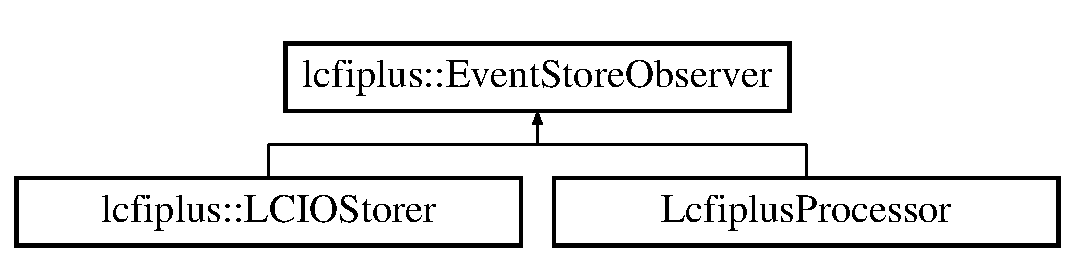
\includegraphics[height=2.000000cm]{classlcfiplus_1_1EventStoreObserver}
\end{center}
\end{figure}
\subsection*{Public Member Functions}
\begin{DoxyCompactItemize}
\item 
{\bf Event\-Store\-Observer} ()
\item 
virtual {\bf $\sim$\-Event\-Store\-Observer} ()
\item 
virtual void {\bf Get\-Callback} (const char $\ast$, const char $\ast$)
\item 
virtual void {\bf Register\-Callback} (const char $\ast$, const char $\ast$, int)
\end{DoxyCompactItemize}


\subsection{Constructor \& Destructor Documentation}
\index{lcfiplus\-::\-Event\-Store\-Observer@{lcfiplus\-::\-Event\-Store\-Observer}!Event\-Store\-Observer@{Event\-Store\-Observer}}
\index{Event\-Store\-Observer@{Event\-Store\-Observer}!lcfiplus::EventStoreObserver@{lcfiplus\-::\-Event\-Store\-Observer}}
\subsubsection[{Event\-Store\-Observer}]{\setlength{\rightskip}{0pt plus 5cm}lcfiplus\-::\-Event\-Store\-Observer\-::\-Event\-Store\-Observer (
\begin{DoxyParamCaption}
{}
\end{DoxyParamCaption}
)\hspace{0.3cm}{\ttfamily [inline]}}\label{classlcfiplus_1_1EventStoreObserver_ab088b5e63835f0e31d6f43b953a3eeb8}
\index{lcfiplus\-::\-Event\-Store\-Observer@{lcfiplus\-::\-Event\-Store\-Observer}!$\sim$\-Event\-Store\-Observer@{$\sim$\-Event\-Store\-Observer}}
\index{$\sim$\-Event\-Store\-Observer@{$\sim$\-Event\-Store\-Observer}!lcfiplus::EventStoreObserver@{lcfiplus\-::\-Event\-Store\-Observer}}
\subsubsection[{$\sim$\-Event\-Store\-Observer}]{\setlength{\rightskip}{0pt plus 5cm}virtual lcfiplus\-::\-Event\-Store\-Observer\-::$\sim$\-Event\-Store\-Observer (
\begin{DoxyParamCaption}
{}
\end{DoxyParamCaption}
)\hspace{0.3cm}{\ttfamily [inline]}, {\ttfamily [virtual]}}\label{classlcfiplus_1_1EventStoreObserver_a3613bf87102daeec979fb48572b31f6d}


\subsection{Member Function Documentation}
\index{lcfiplus\-::\-Event\-Store\-Observer@{lcfiplus\-::\-Event\-Store\-Observer}!Get\-Callback@{Get\-Callback}}
\index{Get\-Callback@{Get\-Callback}!lcfiplus::EventStoreObserver@{lcfiplus\-::\-Event\-Store\-Observer}}
\subsubsection[{Get\-Callback}]{\setlength{\rightskip}{0pt plus 5cm}virtual void lcfiplus\-::\-Event\-Store\-Observer\-::\-Get\-Callback (
\begin{DoxyParamCaption}
\item[{const char $\ast$}]{, }
\item[{const char $\ast$}]{}
\end{DoxyParamCaption}
)\hspace{0.3cm}{\ttfamily [inline]}, {\ttfamily [virtual]}}\label{classlcfiplus_1_1EventStoreObserver_a859fc2e8e0a80224de140f7f8d45ab5f}


Reimplemented in {\bf lcfiplus\-::\-L\-C\-I\-O\-Storer} \doxyref{}{p.}{classlcfiplus_1_1LCIOStorer_a6c8c1ac84052459df7ee7731b0291d2d}.

\index{lcfiplus\-::\-Event\-Store\-Observer@{lcfiplus\-::\-Event\-Store\-Observer}!Register\-Callback@{Register\-Callback}}
\index{Register\-Callback@{Register\-Callback}!lcfiplus::EventStoreObserver@{lcfiplus\-::\-Event\-Store\-Observer}}
\subsubsection[{Register\-Callback}]{\setlength{\rightskip}{0pt plus 5cm}virtual void lcfiplus\-::\-Event\-Store\-Observer\-::\-Register\-Callback (
\begin{DoxyParamCaption}
\item[{const char $\ast$}]{, }
\item[{const char $\ast$}]{, }
\item[{int}]{}
\end{DoxyParamCaption}
)\hspace{0.3cm}{\ttfamily [inline]}, {\ttfamily [virtual]}}\label{classlcfiplus_1_1EventStoreObserver_ab95c097fe767104ff29dad4c2531442f}


Reimplemented in {\bf Lcfiplus\-Processor} \doxyref{}{p.}{classLcfiplusProcessor_a01cfed188f349698ad641092085cf7bf}.



The documentation for this class was generated from the following file\-:\begin{DoxyCompactItemize}
\item 
{\bf Event\-Store.\-h}\end{DoxyCompactItemize}

\section{lcfiplus\-:\-:Exception Class Reference}
\label{classlcfiplus_1_1Exception}\index{lcfiplus\-::\-Exception@{lcfiplus\-::\-Exception}}


{\ttfamily \#include $<$lcfiplus.\-h$>$}

Inheritance diagram for lcfiplus\-:\-:Exception\-:\begin{figure}[H]
\begin{center}
\leavevmode
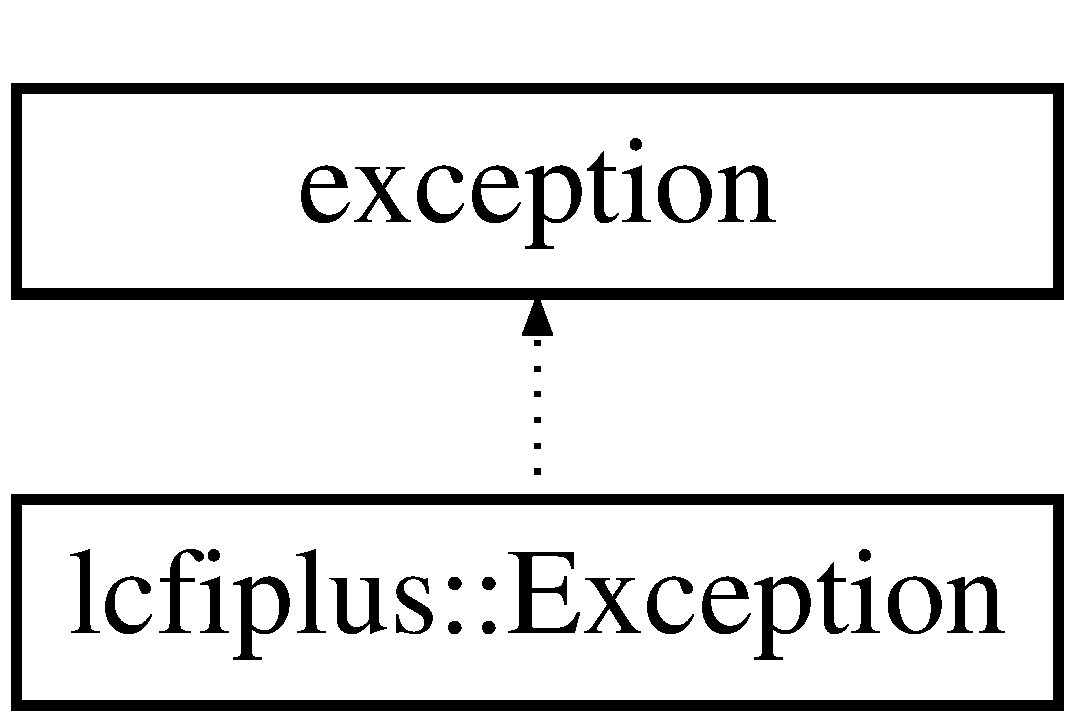
\includegraphics[height=2.000000cm]{classlcfiplus_1_1Exception}
\end{center}
\end{figure}
\subsection*{Public Member Functions}
\begin{DoxyCompactItemize}
\item 
{\bf Exception} (const char $\ast$message)
\item 
virtual {\bf $\sim$\-Exception} ()  throw ()
\item 
virtual const char $\ast$ {\bf what} () const   throw ()
\item 
void {\bf Print} ()
\end{DoxyCompactItemize}


\subsection{Constructor \& Destructor Documentation}
\index{lcfiplus\-::\-Exception@{lcfiplus\-::\-Exception}!Exception@{Exception}}
\index{Exception@{Exception}!lcfiplus::Exception@{lcfiplus\-::\-Exception}}
\subsubsection[{Exception}]{\setlength{\rightskip}{0pt plus 5cm}lcfiplus\-::\-Exception\-::\-Exception (
\begin{DoxyParamCaption}
\item[{const char $\ast$}]{message}
\end{DoxyParamCaption}
)\hspace{0.3cm}{\ttfamily [inline]}}\label{classlcfiplus_1_1Exception_a32454774b1d656e6122afaac99d5e74c}
\index{lcfiplus\-::\-Exception@{lcfiplus\-::\-Exception}!$\sim$\-Exception@{$\sim$\-Exception}}
\index{$\sim$\-Exception@{$\sim$\-Exception}!lcfiplus::Exception@{lcfiplus\-::\-Exception}}
\subsubsection[{$\sim$\-Exception}]{\setlength{\rightskip}{0pt plus 5cm}virtual lcfiplus\-::\-Exception\-::$\sim$\-Exception (
\begin{DoxyParamCaption}
{}
\end{DoxyParamCaption}
) throw  ) \hspace{0.3cm}{\ttfamily [inline]}, {\ttfamily [virtual]}}\label{classlcfiplus_1_1Exception_aa5480d1aa884c98f3a80fe571e74b6b9}


\subsection{Member Function Documentation}
\index{lcfiplus\-::\-Exception@{lcfiplus\-::\-Exception}!Print@{Print}}
\index{Print@{Print}!lcfiplus::Exception@{lcfiplus\-::\-Exception}}
\subsubsection[{Print}]{\setlength{\rightskip}{0pt plus 5cm}void lcfiplus\-::\-Exception\-::\-Print (
\begin{DoxyParamCaption}
{}
\end{DoxyParamCaption}
)\hspace{0.3cm}{\ttfamily [inline]}}\label{classlcfiplus_1_1Exception_a1d9fd6e9354c8e59c515123562794e9a}


Referenced by test\-Suehara().

\index{lcfiplus\-::\-Exception@{lcfiplus\-::\-Exception}!what@{what}}
\index{what@{what}!lcfiplus::Exception@{lcfiplus\-::\-Exception}}
\subsubsection[{what}]{\setlength{\rightskip}{0pt plus 5cm}virtual const char$\ast$ lcfiplus\-::\-Exception\-::what (
\begin{DoxyParamCaption}
{}
\end{DoxyParamCaption}
) const throw  ) \hspace{0.3cm}{\ttfamily [inline]}, {\ttfamily [virtual]}}\label{classlcfiplus_1_1Exception_a381fd14af65bccd6be588f1c5ba6ee42}


Referenced by Lcfiplus\-Processor\-::init(), and Lcfiplus\-Processor\-::process\-Event().



The documentation for this class was generated from the following file\-:\begin{DoxyCompactItemize}
\item 
{\bf lcfiplus.\-h}\end{DoxyCompactItemize}

\section{lcfiplus\-:\-:Flavor\-Tag Class Reference}
\label{classlcfiplus_1_1FlavorTag}\index{lcfiplus\-::\-Flavor\-Tag@{lcfiplus\-::\-Flavor\-Tag}}


Controls the event data and registers and holds algorithms for the computation of flavor tagging variables.  




{\ttfamily \#include $<$Flavor\-Tag.\-h$>$}

Inheritance diagram for lcfiplus\-:\-:Flavor\-Tag\-:\begin{figure}[H]
\begin{center}
\leavevmode
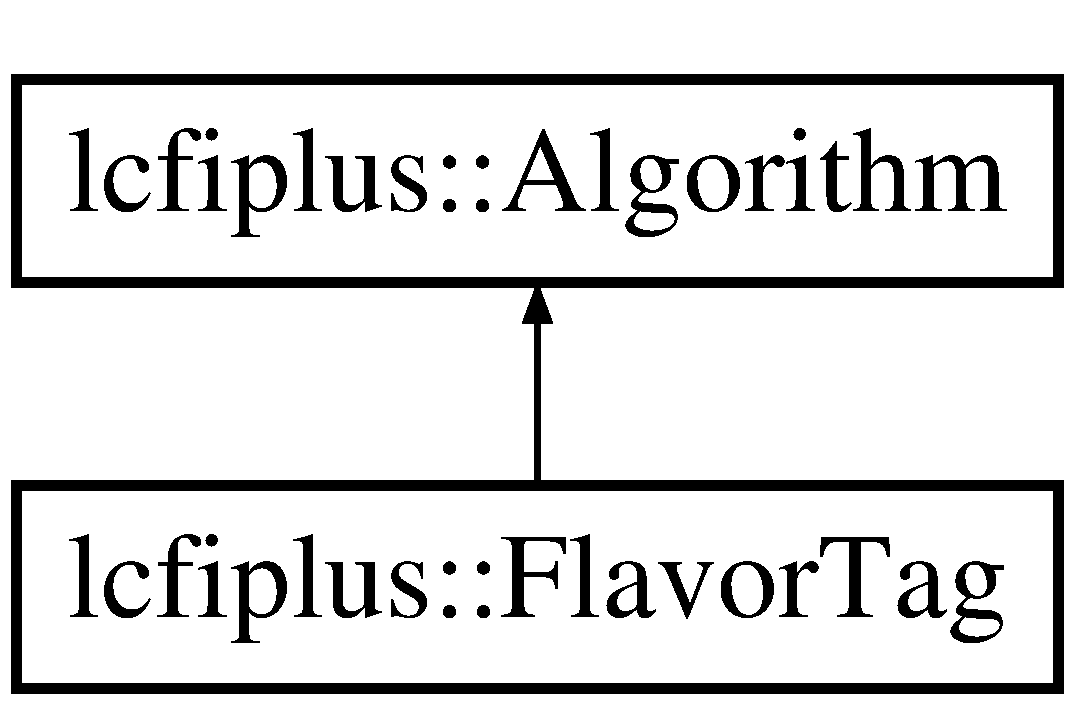
\includegraphics[height=2.000000cm]{classlcfiplus_1_1FlavorTag}
\end{center}
\end{figure}
\subsection*{Public Member Functions}
\begin{DoxyCompactItemize}
\item 
{\bf Flavor\-Tag} ()
\item 
virtual {\bf $\sim$\-Flavor\-Tag} ()
\item 
void {\bf init} ({\bf Parameters} $\ast$param)
\item 
void {\bf process} ()
\item 
void {\bf end} ()
\end{DoxyCompactItemize}
\subsection*{Additional Inherited Members}


\subsection{Detailed Description}
Controls the event data and registers and holds algorithms for the computation of flavor tagging variables. 

This algorithm must be included in the algorithm tag of the X\-M\-L steering file when using any of the flavor tagging features, e.\-g. ntuple production, T\-M\-V\-A training, and evaluation.

\begin{DoxyAuthor}{Author}
T. Tanabe, I\-C\-E\-P\-P, The University of Tokyo 
\end{DoxyAuthor}
\begin{DoxyVersion}{Version}
\$\-Id\$ 
\end{DoxyVersion}


\subsection{Constructor \& Destructor Documentation}
\index{lcfiplus\-::\-Flavor\-Tag@{lcfiplus\-::\-Flavor\-Tag}!Flavor\-Tag@{Flavor\-Tag}}
\index{Flavor\-Tag@{Flavor\-Tag}!lcfiplus::FlavorTag@{lcfiplus\-::\-Flavor\-Tag}}
\subsubsection[{Flavor\-Tag}]{\setlength{\rightskip}{0pt plus 5cm}lcfiplus\-::\-Flavor\-Tag\-::\-Flavor\-Tag (
\begin{DoxyParamCaption}
{}
\end{DoxyParamCaption}
)\hspace{0.3cm}{\ttfamily [inline]}}\label{classlcfiplus_1_1FlavorTag_a14c03cd001e5a3f7899b9cc4c3d03f39}
\index{lcfiplus\-::\-Flavor\-Tag@{lcfiplus\-::\-Flavor\-Tag}!$\sim$\-Flavor\-Tag@{$\sim$\-Flavor\-Tag}}
\index{$\sim$\-Flavor\-Tag@{$\sim$\-Flavor\-Tag}!lcfiplus::FlavorTag@{lcfiplus\-::\-Flavor\-Tag}}
\subsubsection[{$\sim$\-Flavor\-Tag}]{\setlength{\rightskip}{0pt plus 5cm}virtual lcfiplus\-::\-Flavor\-Tag\-::$\sim$\-Flavor\-Tag (
\begin{DoxyParamCaption}
{}
\end{DoxyParamCaption}
)\hspace{0.3cm}{\ttfamily [inline]}, {\ttfamily [virtual]}}\label{classlcfiplus_1_1FlavorTag_ad8077e1d901a7ea3c4f1c6e92a032320}


\subsection{Member Function Documentation}
\index{lcfiplus\-::\-Flavor\-Tag@{lcfiplus\-::\-Flavor\-Tag}!end@{end}}
\index{end@{end}!lcfiplus::FlavorTag@{lcfiplus\-::\-Flavor\-Tag}}
\subsubsection[{end}]{\setlength{\rightskip}{0pt plus 5cm}void lcfiplus\-::\-Flavor\-Tag\-::end (
\begin{DoxyParamCaption}
{}
\end{DoxyParamCaption}
)\hspace{0.3cm}{\ttfamily [virtual]}}\label{classlcfiplus_1_1FlavorTag_abd9ac826b60d9c51d3ed8d7cf02de074}


Reimplemented from {\bf lcfiplus\-::\-Algorithm} \doxyref{}{p.}{classlcfiplus_1_1Algorithm_a4276b93869d614f59eef92b8c728ef60}.

\index{lcfiplus\-::\-Flavor\-Tag@{lcfiplus\-::\-Flavor\-Tag}!init@{init}}
\index{init@{init}!lcfiplus::FlavorTag@{lcfiplus\-::\-Flavor\-Tag}}
\subsubsection[{init}]{\setlength{\rightskip}{0pt plus 5cm}void lcfiplus\-::\-Flavor\-Tag\-::init (
\begin{DoxyParamCaption}
\item[{{\bf Parameters} $\ast$}]{param}
\end{DoxyParamCaption}
)\hspace{0.3cm}{\ttfamily [virtual]}}\label{classlcfiplus_1_1FlavorTag_aa872596e47fd0e4ac56b70e144d9408e}


Reimplemented from {\bf lcfiplus\-::\-Algorithm} \doxyref{}{p.}{classlcfiplus_1_1Algorithm_a178a273b9976b87f182190f4250cac9e}.



References lcfiplus\-::\-Parameters\-::get(), lcfiplus\-::\-F\-T\-Manager\-::get\-Instance(), lcfiplus\-::\-Algorithm\-::init(), lcfiplus\-::\-F\-T\-Manager\-::init\-Vars(), lcfiplus\-::\-Event\-::\-Instance(), and lcfiplus\-::\-Event\-::set\-Default\-Primary\-Vertex().

\index{lcfiplus\-::\-Flavor\-Tag@{lcfiplus\-::\-Flavor\-Tag}!process@{process}}
\index{process@{process}!lcfiplus::FlavorTag@{lcfiplus\-::\-Flavor\-Tag}}
\subsubsection[{process}]{\setlength{\rightskip}{0pt plus 5cm}void lcfiplus\-::\-Flavor\-Tag\-::process (
\begin{DoxyParamCaption}
{}
\end{DoxyParamCaption}
)\hspace{0.3cm}{\ttfamily [virtual]}}\label{classlcfiplus_1_1FlavorTag_a44be9eb8162b2daabd06907c39098d33}


Implements {\bf lcfiplus\-::\-Algorithm} \doxyref{}{p.}{classlcfiplus_1_1Algorithm_a628e1509b55b2cda1e2640b58be6ce6f}.



References lcfiplus\-::\-F\-T\-Manager\-::get\-Instance(), lcfiplus\-::\-Event\-::\-Instance(), lcfiplus\-::\-F\-T\-Manager\-::process(), lcfiplus\-::\-F\-T\-Manager\-::set\-Auxiliary(), and lcfiplus\-::\-F\-T\-Manager\-::set\-I\-P\-Prob\-Holder().



The documentation for this class was generated from the following files\-:\begin{DoxyCompactItemize}
\item 
{\bf Flavor\-Tag.\-h}\item 
{\bf Flavor\-Tag.\-cc}\end{DoxyCompactItemize}

\section{lcfiplus\-:\-:Flavtag\-Category Struct Reference}
\label{structlcfiplus_1_1FlavtagCategory}\index{lcfiplus\-::\-Flavtag\-Category@{lcfiplus\-::\-Flavtag\-Category}}


{\ttfamily \#include $<$flavtag.\-h$>$}

\subsection*{Public Member Functions}
\begin{DoxyCompactItemize}
\item 
void {\bf Add\-Variable} (std\-::string s, char)
\item 
void {\bf Add\-Spectator} (std\-::string s)
\end{DoxyCompactItemize}
\subsection*{Public Attributes}
\begin{DoxyCompactItemize}
\item 
T\-String {\bf definition}
\item 
T\-String {\bf preselection}
\item 
std\-::vector$<$ std\-::string $>$ {\bf vars}
\item 
std\-::vector$<$ std\-::string $>$ {\bf spec}
\end{DoxyCompactItemize}


\subsection{Member Function Documentation}
\index{lcfiplus\-::\-Flavtag\-Category@{lcfiplus\-::\-Flavtag\-Category}!Add\-Spectator@{Add\-Spectator}}
\index{Add\-Spectator@{Add\-Spectator}!lcfiplus::FlavtagCategory@{lcfiplus\-::\-Flavtag\-Category}}
\subsubsection[{Add\-Spectator}]{\setlength{\rightskip}{0pt plus 5cm}void lcfiplus\-::\-Flavtag\-Category\-::\-Add\-Spectator (
\begin{DoxyParamCaption}
\item[{std\-::string}]{s}
\end{DoxyParamCaption}
)\hspace{0.3cm}{\ttfamily [inline]}}\label{structlcfiplus_1_1FlavtagCategory_a2fbbca0a85a4abf905d5c40ec7309db4}


References spec.

\index{lcfiplus\-::\-Flavtag\-Category@{lcfiplus\-::\-Flavtag\-Category}!Add\-Variable@{Add\-Variable}}
\index{Add\-Variable@{Add\-Variable}!lcfiplus::FlavtagCategory@{lcfiplus\-::\-Flavtag\-Category}}
\subsubsection[{Add\-Variable}]{\setlength{\rightskip}{0pt plus 5cm}void lcfiplus\-::\-Flavtag\-Category\-::\-Add\-Variable (
\begin{DoxyParamCaption}
\item[{std\-::string}]{s, }
\item[{char}]{}
\end{DoxyParamCaption}
)\hspace{0.3cm}{\ttfamily [inline]}}\label{structlcfiplus_1_1FlavtagCategory_a4d9be1da44e5d6abb7f7638aae7833c7}


References vars.



\subsection{Member Data Documentation}
\index{lcfiplus\-::\-Flavtag\-Category@{lcfiplus\-::\-Flavtag\-Category}!definition@{definition}}
\index{definition@{definition}!lcfiplus::FlavtagCategory@{lcfiplus\-::\-Flavtag\-Category}}
\subsubsection[{definition}]{\setlength{\rightskip}{0pt plus 5cm}T\-String lcfiplus\-::\-Flavtag\-Category\-::definition}\label{structlcfiplus_1_1FlavtagCategory_a5ff949e40f053671861538f57caea455}


Referenced by lcfiplus\-::\-Train\-M\-V\-A\-::end(), lcfiplus\-::\-Train\-M\-V\-A\-::init(), and lcfiplus\-::\-Read\-M\-V\-A\-::init().

\index{lcfiplus\-::\-Flavtag\-Category@{lcfiplus\-::\-Flavtag\-Category}!preselection@{preselection}}
\index{preselection@{preselection}!lcfiplus::FlavtagCategory@{lcfiplus\-::\-Flavtag\-Category}}
\subsubsection[{preselection}]{\setlength{\rightskip}{0pt plus 5cm}T\-String lcfiplus\-::\-Flavtag\-Category\-::preselection}\label{structlcfiplus_1_1FlavtagCategory_a3801d17f9bb0595ba0da547a4d7f261b}


Referenced by lcfiplus\-::\-Train\-M\-V\-A\-::end(), lcfiplus\-::\-Train\-M\-V\-A\-::init(), and lcfiplus\-::\-Read\-M\-V\-A\-::init().

\index{lcfiplus\-::\-Flavtag\-Category@{lcfiplus\-::\-Flavtag\-Category}!spec@{spec}}
\index{spec@{spec}!lcfiplus::FlavtagCategory@{lcfiplus\-::\-Flavtag\-Category}}
\subsubsection[{spec}]{\setlength{\rightskip}{0pt plus 5cm}std\-::vector$<$std\-::string$>$ lcfiplus\-::\-Flavtag\-Category\-::spec}\label{structlcfiplus_1_1FlavtagCategory_a5d70094f45fcd7b7ae75d9ec2f309948}


Referenced by Add\-Spectator(), lcfiplus\-::\-Train\-M\-V\-A\-::end(), lcfiplus\-::\-Train\-M\-V\-A\-::init(), and lcfiplus\-::\-Read\-M\-V\-A\-::init().

\index{lcfiplus\-::\-Flavtag\-Category@{lcfiplus\-::\-Flavtag\-Category}!vars@{vars}}
\index{vars@{vars}!lcfiplus::FlavtagCategory@{lcfiplus\-::\-Flavtag\-Category}}
\subsubsection[{vars}]{\setlength{\rightskip}{0pt plus 5cm}std\-::vector$<$std\-::string$>$ lcfiplus\-::\-Flavtag\-Category\-::vars}\label{structlcfiplus_1_1FlavtagCategory_a00016d50d6a8a41b087a55083e0e5be6}


Referenced by Add\-Variable(), lcfiplus\-::\-Train\-M\-V\-A\-::end(), lcfiplus\-::\-Train\-M\-V\-A\-::init(), and lcfiplus\-::\-Read\-M\-V\-A\-::init().



The documentation for this struct was generated from the following file\-:\begin{DoxyCompactItemize}
\item 
{\bf flavtag.\-h}\end{DoxyCompactItemize}

\section{lcfiplus\-:\-:Flavtag\-Reader Class Reference}
\label{classlcfiplus_1_1FlavtagReader}\index{lcfiplus\-::\-Flavtag\-Reader@{lcfiplus\-::\-Flavtag\-Reader}}


{\ttfamily \#include $<$testproc.\-h$>$}

Inheritance diagram for lcfiplus\-:\-:Flavtag\-Reader\-:\begin{figure}[H]
\begin{center}
\leavevmode
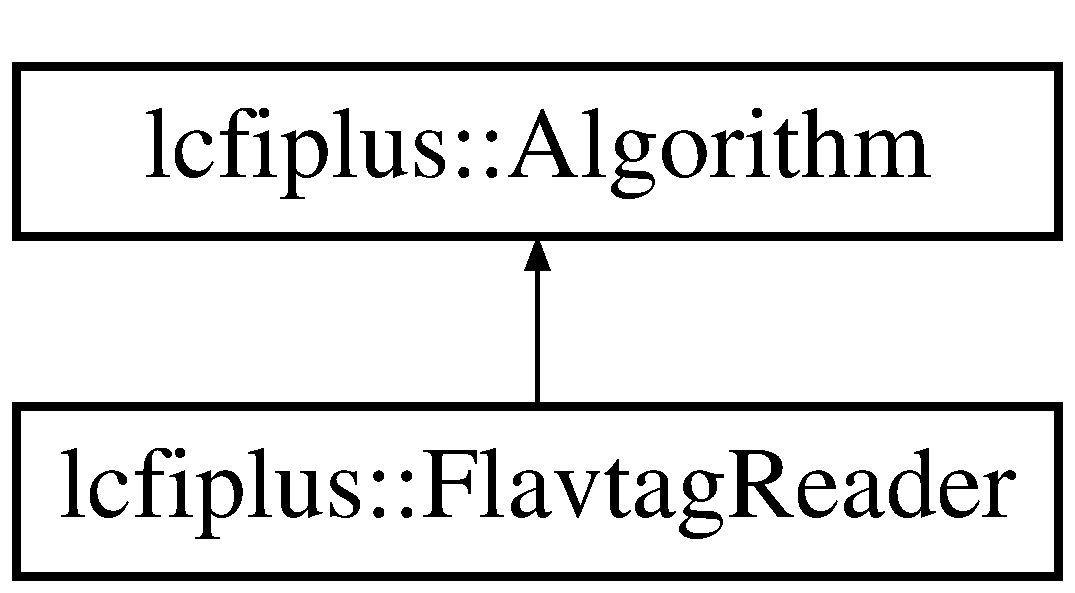
\includegraphics[height=2.000000cm]{classlcfiplus_1_1FlavtagReader}
\end{center}
\end{figure}
\subsection*{Public Member Functions}
\begin{DoxyCompactItemize}
\item 
{\bf Flavtag\-Reader} ()
\item 
virtual {\bf $\sim$\-Flavtag\-Reader} ()
\item 
void {\bf init} ({\bf Parameters} $\ast$param)
\item 
void {\bf process} ()
\item 
void {\bf end} ()
\item 
{\bf Class\-Def} ({\bf Flavtag\-Reader}, 1)
\end{DoxyCompactItemize}
\subsection*{Additional Inherited Members}


\subsection{Constructor \& Destructor Documentation}
\index{lcfiplus\-::\-Flavtag\-Reader@{lcfiplus\-::\-Flavtag\-Reader}!Flavtag\-Reader@{Flavtag\-Reader}}
\index{Flavtag\-Reader@{Flavtag\-Reader}!lcfiplus::FlavtagReader@{lcfiplus\-::\-Flavtag\-Reader}}
\subsubsection[{Flavtag\-Reader}]{\setlength{\rightskip}{0pt plus 5cm}lcfiplus\-::\-Flavtag\-Reader\-::\-Flavtag\-Reader (
\begin{DoxyParamCaption}
{}
\end{DoxyParamCaption}
)\hspace{0.3cm}{\ttfamily [inline]}}\label{classlcfiplus_1_1FlavtagReader_a6f17f1b93760938879f76e85299da988}
\index{lcfiplus\-::\-Flavtag\-Reader@{lcfiplus\-::\-Flavtag\-Reader}!$\sim$\-Flavtag\-Reader@{$\sim$\-Flavtag\-Reader}}
\index{$\sim$\-Flavtag\-Reader@{$\sim$\-Flavtag\-Reader}!lcfiplus::FlavtagReader@{lcfiplus\-::\-Flavtag\-Reader}}
\subsubsection[{$\sim$\-Flavtag\-Reader}]{\setlength{\rightskip}{0pt plus 5cm}virtual lcfiplus\-::\-Flavtag\-Reader\-::$\sim$\-Flavtag\-Reader (
\begin{DoxyParamCaption}
{}
\end{DoxyParamCaption}
)\hspace{0.3cm}{\ttfamily [inline]}, {\ttfamily [virtual]}}\label{classlcfiplus_1_1FlavtagReader_a0ef2fdd86266981aef4068337c5070df}


\subsection{Member Function Documentation}
\index{lcfiplus\-::\-Flavtag\-Reader@{lcfiplus\-::\-Flavtag\-Reader}!Class\-Def@{Class\-Def}}
\index{Class\-Def@{Class\-Def}!lcfiplus::FlavtagReader@{lcfiplus\-::\-Flavtag\-Reader}}
\subsubsection[{Class\-Def}]{\setlength{\rightskip}{0pt plus 5cm}lcfiplus\-::\-Flavtag\-Reader\-::\-Class\-Def (
\begin{DoxyParamCaption}
\item[{{\bf Flavtag\-Reader}}]{, }
\item[{1}]{}
\end{DoxyParamCaption}
)}\label{classlcfiplus_1_1FlavtagReader_a2e473bdee34466be0746c781ff38d303}
\index{lcfiplus\-::\-Flavtag\-Reader@{lcfiplus\-::\-Flavtag\-Reader}!end@{end}}
\index{end@{end}!lcfiplus::FlavtagReader@{lcfiplus\-::\-Flavtag\-Reader}}
\subsubsection[{end}]{\setlength{\rightskip}{0pt plus 5cm}void lcfiplus\-::\-Flavtag\-Reader\-::end (
\begin{DoxyParamCaption}
{}
\end{DoxyParamCaption}
)\hspace{0.3cm}{\ttfamily [virtual]}}\label{classlcfiplus_1_1FlavtagReader_a6b4aeb451123b3fa850a24730f0f12b7}


Reimplemented from {\bf lcfiplus\-::\-Algorithm} \doxyref{}{p.}{classlcfiplus_1_1Algorithm_a4276b93869d614f59eef92b8c728ef60}.

\index{lcfiplus\-::\-Flavtag\-Reader@{lcfiplus\-::\-Flavtag\-Reader}!init@{init}}
\index{init@{init}!lcfiplus::FlavtagReader@{lcfiplus\-::\-Flavtag\-Reader}}
\subsubsection[{init}]{\setlength{\rightskip}{0pt plus 5cm}void lcfiplus\-::\-Flavtag\-Reader\-::init (
\begin{DoxyParamCaption}
\item[{{\bf Parameters} $\ast$}]{param}
\end{DoxyParamCaption}
)\hspace{0.3cm}{\ttfamily [virtual]}}\label{classlcfiplus_1_1FlavtagReader_a5b72270f230113bf33924453f8149fed}


Reimplemented from {\bf lcfiplus\-::\-Algorithm} \doxyref{}{p.}{classlcfiplus_1_1Algorithm_a178a273b9976b87f182190f4250cac9e}.



References lcfiplus\-::\-Parameters\-::get(), lcfiplus\-::\-Algorithm\-::init(), lcfiplus\-::\-Event\-::\-Instance(), and lcfiplus\-::\-Event\-::set\-Default\-Primary\-Vertex().

\index{lcfiplus\-::\-Flavtag\-Reader@{lcfiplus\-::\-Flavtag\-Reader}!process@{process}}
\index{process@{process}!lcfiplus::FlavtagReader@{lcfiplus\-::\-Flavtag\-Reader}}
\subsubsection[{process}]{\setlength{\rightskip}{0pt plus 5cm}void lcfiplus\-::\-Flavtag\-Reader\-::process (
\begin{DoxyParamCaption}
{}
\end{DoxyParamCaption}
)\hspace{0.3cm}{\ttfamily [virtual]}}\label{classlcfiplus_1_1FlavtagReader_a7cd1aca9d0bd08130f8f965de9fdaed7}


Implements {\bf lcfiplus\-::\-Algorithm} \doxyref{}{p.}{classlcfiplus_1_1Algorithm_a628e1509b55b2cda1e2640b58be6ce6f}.



References lcfiplus\-::\-Event\-Store\-::\-Get(), lcfiplus\-::\-Parameters\-::get(), lcfiplus\-::\-Jet\-::get\-Param(), and lcfiplus\-::\-Event\-::\-Instance().



The documentation for this class was generated from the following files\-:\begin{DoxyCompactItemize}
\item 
{\bf testproc.\-h}\item 
{\bf testproc.\-cc}\end{DoxyCompactItemize}

\section{lcfiplus\-:\-:Flavtag\-Type Struct Reference}
\label{structlcfiplus_1_1FlavtagType}\index{lcfiplus\-::\-Flavtag\-Type@{lcfiplus\-::\-Flavtag\-Type}}


{\ttfamily \#include $<$flavtag.\-h$>$}

\subsection*{Public Attributes}
\begin{DoxyCompactItemize}
\item 
T\-String {\bf name}
\item 
T\-String {\bf cut}
\end{DoxyCompactItemize}


\subsection{Member Data Documentation}
\index{lcfiplus\-::\-Flavtag\-Type@{lcfiplus\-::\-Flavtag\-Type}!cut@{cut}}
\index{cut@{cut}!lcfiplus::FlavtagType@{lcfiplus\-::\-Flavtag\-Type}}
\subsubsection[{cut}]{\setlength{\rightskip}{0pt plus 5cm}T\-String lcfiplus\-::\-Flavtag\-Type\-::cut}\label{structlcfiplus_1_1FlavtagType_a5f9e0f11aacc3b9ef1fdce68fe2ffda3}
\index{lcfiplus\-::\-Flavtag\-Type@{lcfiplus\-::\-Flavtag\-Type}!name@{name}}
\index{name@{name}!lcfiplus::FlavtagType@{lcfiplus\-::\-Flavtag\-Type}}
\subsubsection[{name}]{\setlength{\rightskip}{0pt plus 5cm}T\-String lcfiplus\-::\-Flavtag\-Type\-::name}\label{structlcfiplus_1_1FlavtagType_a41acddbb497954e875416c16648c0b08}


The documentation for this struct was generated from the following file\-:\begin{DoxyCompactItemize}
\item 
{\bf flavtag.\-h}\end{DoxyCompactItemize}

\section{lcfiplus\-:\-:Ft1\-Vtx\-Prob Class Reference}
\label{classlcfiplus_1_1Ft1VtxProb}\index{lcfiplus\-::\-Ft1\-Vtx\-Prob@{lcfiplus\-::\-Ft1\-Vtx\-Prob}}
Inheritance diagram for lcfiplus\-:\-:Ft1\-Vtx\-Prob\-:\begin{figure}[H]
\begin{center}
\leavevmode
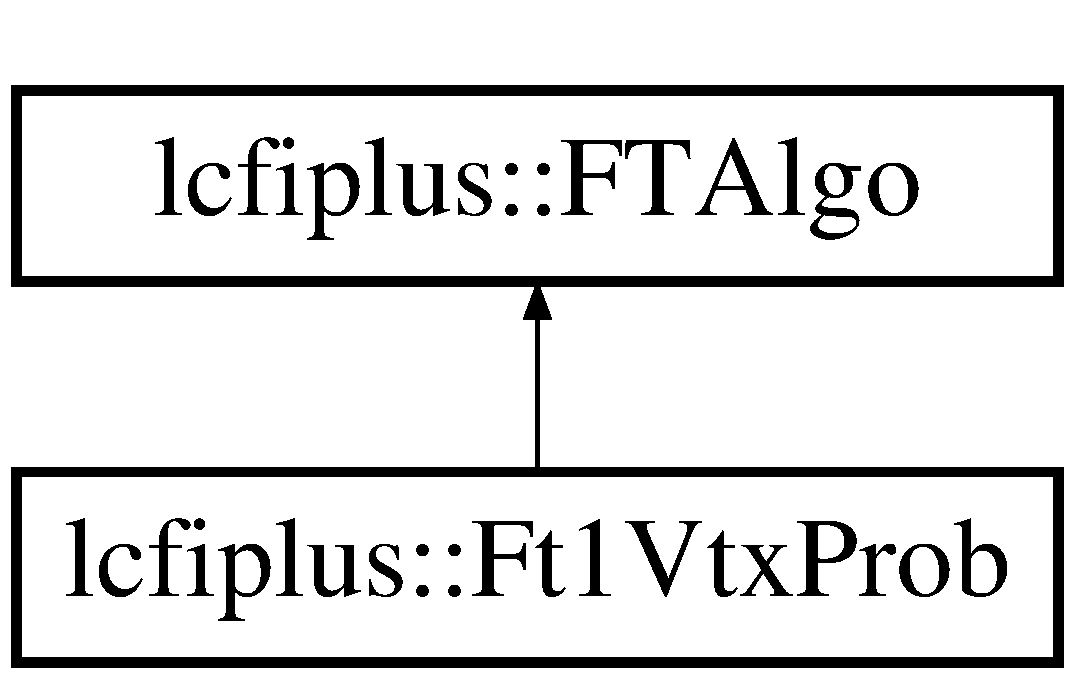
\includegraphics[height=2.000000cm]{classlcfiplus_1_1Ft1VtxProb}
\end{center}
\end{figure}
\subsection*{Public Member Functions}
\begin{DoxyCompactItemize}
\item 
{\bf Ft1\-Vtx\-Prob} ()
\item 
void {\bf process} ()
\end{DoxyCompactItemize}
\subsection*{Additional Inherited Members}


\subsection{Constructor \& Destructor Documentation}
\index{lcfiplus\-::\-Ft1\-Vtx\-Prob@{lcfiplus\-::\-Ft1\-Vtx\-Prob}!Ft1\-Vtx\-Prob@{Ft1\-Vtx\-Prob}}
\index{Ft1\-Vtx\-Prob@{Ft1\-Vtx\-Prob}!lcfiplus::Ft1VtxProb@{lcfiplus\-::\-Ft1\-Vtx\-Prob}}
\subsubsection[{Ft1\-Vtx\-Prob}]{\setlength{\rightskip}{0pt plus 5cm}lcfiplus\-::\-Ft1\-Vtx\-Prob\-::\-Ft1\-Vtx\-Prob (
\begin{DoxyParamCaption}
{}
\end{DoxyParamCaption}
)\hspace{0.3cm}{\ttfamily [inline]}}\label{classlcfiplus_1_1Ft1VtxProb_abf316d895e1914a6e534353df264a2b5}


\subsection{Member Function Documentation}
\index{lcfiplus\-::\-Ft1\-Vtx\-Prob@{lcfiplus\-::\-Ft1\-Vtx\-Prob}!process@{process}}
\index{process@{process}!lcfiplus::Ft1VtxProb@{lcfiplus\-::\-Ft1\-Vtx\-Prob}}
\subsubsection[{process}]{\setlength{\rightskip}{0pt plus 5cm}void lcfiplus\-::\-Ft1\-Vtx\-Prob\-::process (
\begin{DoxyParamCaption}
{}
\end{DoxyParamCaption}
)\hspace{0.3cm}{\ttfamily [inline]}, {\ttfamily [virtual]}}\label{classlcfiplus_1_1Ft1VtxProb_ad74ede9d41a8727cd2aae354d1690743}


Reimplemented from {\bf lcfiplus\-::\-F\-T\-Algo} \doxyref{}{p.}{classlcfiplus_1_1FTAlgo_a23cc3f3cd1c100ab6b5e16056112351a}.



References lcfiplus\-::\-Vertex\-::get\-Prob().



The documentation for this class was generated from the following file\-:\begin{DoxyCompactItemize}
\item 
{\bf Flavor\-Tag.\-cc}\end{DoxyCompactItemize}

\section{lcfiplus\-:\-:F\-T\-Algo Class Reference}
\label{classlcfiplus_1_1FTAlgo}\index{lcfiplus\-::\-F\-T\-Algo@{lcfiplus\-::\-F\-T\-Algo}}


{\ttfamily \#include $<$flavtag.\-h$>$}

Inheritance diagram for lcfiplus\-:\-:F\-T\-Algo\-:\begin{figure}[H]
\begin{center}
\leavevmode
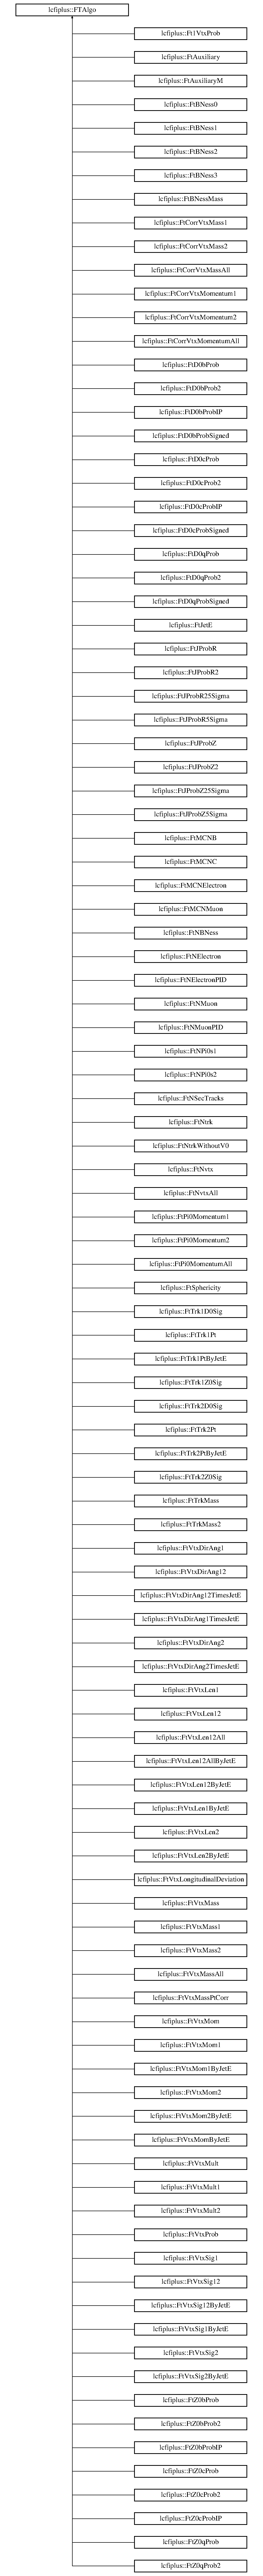
\includegraphics[height=12.000000cm]{classlcfiplus_1_1FTAlgo}
\end{center}
\end{figure}
\subsection*{Public Member Functions}
\begin{DoxyCompactItemize}
\item 
{\bf F\-T\-Algo} (string name)
\item 
virtual {\bf $\sim$\-F\-T\-Algo} ()
\item 
void {\bf set\-Event} (const {\bf Event} $\ast$event, const {\bf Vertex} $\ast$privtx)
\item 
void {\bf set\-Jet} (const {\bf Jet} $\ast$jet)
\item 
void {\bf set\-N\-Hits\-Joint\-Prob\-D0} (int value)
\item 
void {\bf set\-N\-Hits\-Joint\-Prob\-Z0} (int value)
\item 
void {\bf set\-N\-Hits\-Most\-Significant\-Track} (int value)
\item 
float {\bf get\-Value} ()
\item 
const string \& {\bf get\-Name} () const 
\item 
float $\ast$ {\bf get\-Value\-Address} ()
\item 
virtual void {\bf process\-Event} ()
\item 
virtual void {\bf process} ()
\end{DoxyCompactItemize}
\subsection*{Protected Attributes}
\begin{DoxyCompactItemize}
\item 
const {\bf Event} $\ast$ {\bf \-\_\-event}
\item 
const {\bf Vertex} $\ast$ {\bf \-\_\-privtx}
\item 
const {\bf Jet} $\ast$ {\bf \-\_\-jet}
\item 
int {\bf \-\_\-nhits\-Joint\-Prob\-D0}
\item 
int {\bf \-\_\-nhits\-Joint\-Prob\-Z0}
\item 
int {\bf \-\_\-nhits\-Most\-Significant\-Track}
\item 
float {\bf \-\_\-result}
\item 
string {\bf \-\_\-name}
\end{DoxyCompactItemize}


\subsection{Constructor \& Destructor Documentation}
\index{lcfiplus\-::\-F\-T\-Algo@{lcfiplus\-::\-F\-T\-Algo}!F\-T\-Algo@{F\-T\-Algo}}
\index{F\-T\-Algo@{F\-T\-Algo}!lcfiplus::FTAlgo@{lcfiplus\-::\-F\-T\-Algo}}
\subsubsection[{F\-T\-Algo}]{\setlength{\rightskip}{0pt plus 5cm}lcfiplus\-::\-F\-T\-Algo\-::\-F\-T\-Algo (
\begin{DoxyParamCaption}
\item[{string}]{name}
\end{DoxyParamCaption}
)\hspace{0.3cm}{\ttfamily [inline]}}\label{classlcfiplus_1_1FTAlgo_a18309a8c94ce19e288f03d48cfe00e79}
\index{lcfiplus\-::\-F\-T\-Algo@{lcfiplus\-::\-F\-T\-Algo}!$\sim$\-F\-T\-Algo@{$\sim$\-F\-T\-Algo}}
\index{$\sim$\-F\-T\-Algo@{$\sim$\-F\-T\-Algo}!lcfiplus::FTAlgo@{lcfiplus\-::\-F\-T\-Algo}}
\subsubsection[{$\sim$\-F\-T\-Algo}]{\setlength{\rightskip}{0pt plus 5cm}virtual lcfiplus\-::\-F\-T\-Algo\-::$\sim$\-F\-T\-Algo (
\begin{DoxyParamCaption}
{}
\end{DoxyParamCaption}
)\hspace{0.3cm}{\ttfamily [inline]}, {\ttfamily [virtual]}}\label{classlcfiplus_1_1FTAlgo_af267a08fa8ee5359a53dcd8758828dbd}


\subsection{Member Function Documentation}
\index{lcfiplus\-::\-F\-T\-Algo@{lcfiplus\-::\-F\-T\-Algo}!get\-Name@{get\-Name}}
\index{get\-Name@{get\-Name}!lcfiplus::FTAlgo@{lcfiplus\-::\-F\-T\-Algo}}
\subsubsection[{get\-Name}]{\setlength{\rightskip}{0pt plus 5cm}const string\& lcfiplus\-::\-F\-T\-Algo\-::get\-Name (
\begin{DoxyParamCaption}
{}
\end{DoxyParamCaption}
) const\hspace{0.3cm}{\ttfamily [inline]}}\label{classlcfiplus_1_1FTAlgo_ac919ac2ff0871dcb896ff871bd6bf4fc}


References \-\_\-name.



Referenced by lcfiplus\-::\-F\-T\-Manager\-::get\-Var\-Address(), lcfiplus\-::\-F\-T\-Manager\-::open\-File(), lcfiplus\-::\-F\-T\-Manager\-::open\-Tree(), and lcfiplus\-::\-F\-T\-Manager\-::process().

\index{lcfiplus\-::\-F\-T\-Algo@{lcfiplus\-::\-F\-T\-Algo}!get\-Value@{get\-Value}}
\index{get\-Value@{get\-Value}!lcfiplus::FTAlgo@{lcfiplus\-::\-F\-T\-Algo}}
\subsubsection[{get\-Value}]{\setlength{\rightskip}{0pt plus 5cm}float lcfiplus\-::\-F\-T\-Algo\-::get\-Value (
\begin{DoxyParamCaption}
{}
\end{DoxyParamCaption}
)}\label{classlcfiplus_1_1FTAlgo_acee17e9515c3ca59b50eae41490c29de}


References \-\_\-result.

\index{lcfiplus\-::\-F\-T\-Algo@{lcfiplus\-::\-F\-T\-Algo}!get\-Value\-Address@{get\-Value\-Address}}
\index{get\-Value\-Address@{get\-Value\-Address}!lcfiplus::FTAlgo@{lcfiplus\-::\-F\-T\-Algo}}
\subsubsection[{get\-Value\-Address}]{\setlength{\rightskip}{0pt plus 5cm}float$\ast$ lcfiplus\-::\-F\-T\-Algo\-::get\-Value\-Address (
\begin{DoxyParamCaption}
{}
\end{DoxyParamCaption}
)\hspace{0.3cm}{\ttfamily [inline]}}\label{classlcfiplus_1_1FTAlgo_a61f8d2c2afe4f4d563c43cb0817047e0}


References \-\_\-result.



Referenced by lcfiplus\-::\-F\-T\-Manager\-::get\-Var\-Address(), lcfiplus\-::\-F\-T\-Manager\-::open\-File(), and lcfiplus\-::\-F\-T\-Manager\-::open\-Tree().

\index{lcfiplus\-::\-F\-T\-Algo@{lcfiplus\-::\-F\-T\-Algo}!process@{process}}
\index{process@{process}!lcfiplus::FTAlgo@{lcfiplus\-::\-F\-T\-Algo}}
\subsubsection[{process}]{\setlength{\rightskip}{0pt plus 5cm}virtual void lcfiplus\-::\-F\-T\-Algo\-::process (
\begin{DoxyParamCaption}
{}
\end{DoxyParamCaption}
)\hspace{0.3cm}{\ttfamily [inline]}, {\ttfamily [virtual]}}\label{classlcfiplus_1_1FTAlgo_a23cc3f3cd1c100ab6b5e16056112351a}


Reimplemented in {\bf lcfiplus\-::\-Ft\-N\-B\-Ness} \doxyref{}{p.}{classlcfiplus_1_1FtNBNess_af9a1114a1d0f001a10036490570e5a82}, {\bf lcfiplus\-::\-Ft\-B\-Ness\-Mass} \doxyref{}{p.}{classlcfiplus_1_1FtBNessMass_aa542017c9cce9c344b674aae68f3084e}, {\bf lcfiplus\-::\-Ft\-B\-Ness3} \doxyref{}{p.}{classlcfiplus_1_1FtBNess3_aea7ab74de348d9897b3804d12bd4f938}, {\bf lcfiplus\-::\-Ft\-B\-Ness2} \doxyref{}{p.}{classlcfiplus_1_1FtBNess2_a777253ce5623451441076e1f82db65d7}, {\bf lcfiplus\-::\-Ft\-B\-Ness1} \doxyref{}{p.}{classlcfiplus_1_1FtBNess1_a91ff1353e4e18811aece7512160fd116}, {\bf lcfiplus\-::\-Ft\-B\-Ness0} \doxyref{}{p.}{classlcfiplus_1_1FtBNess0_af8d04b8f7e900520ee4057ad9d27b40f}, {\bf lcfiplus\-::\-Ft\-N\-Pi0s2} \doxyref{}{p.}{classlcfiplus_1_1FtNPi0s2_a924b3a544cab8451465c7d33e7480b87}, {\bf lcfiplus\-::\-Ft\-N\-Pi0s1} \doxyref{}{p.}{classlcfiplus_1_1FtNPi0s1_a7fdafff17efcbeabf1697488b99cbeae}, {\bf lcfiplus\-::\-Ft\-Pi0\-Momentum\-All} \doxyref{}{p.}{classlcfiplus_1_1FtPi0MomentumAll_aac1d58ec21b23c22524859dd71c950c1}, {\bf lcfiplus\-::\-Ft\-Pi0\-Momentum2} \doxyref{}{p.}{classlcfiplus_1_1FtPi0Momentum2_aa676b1d5afd4581dabf344232dca8bb9}, {\bf lcfiplus\-::\-Ft\-Pi0\-Momentum1} \doxyref{}{p.}{classlcfiplus_1_1FtPi0Momentum1_a28c14c5071b349004b59be4e389713e0}, {\bf lcfiplus\-::\-Ft\-Corr\-Vtx\-Momentum\-All} \doxyref{}{p.}{classlcfiplus_1_1FtCorrVtxMomentumAll_a541350ba8ec892f2d86b3072d2b5e3ad}, {\bf lcfiplus\-::\-Ft\-Corr\-Vtx\-Momentum2} \doxyref{}{p.}{classlcfiplus_1_1FtCorrVtxMomentum2_a3bbf00a47a5598287aedffbcd7f1f4e7}, {\bf lcfiplus\-::\-Ft\-Corr\-Vtx\-Momentum1} \doxyref{}{p.}{classlcfiplus_1_1FtCorrVtxMomentum1_aed6efc62695091f145b3ee80d8d0bbc0}, {\bf lcfiplus\-::\-Ft\-Corr\-Vtx\-Mass\-All} \doxyref{}{p.}{classlcfiplus_1_1FtCorrVtxMassAll_a2a48b21fd4d03f7c35bbe71040cec7c9}, {\bf lcfiplus\-::\-Ft\-Corr\-Vtx\-Mass2} \doxyref{}{p.}{classlcfiplus_1_1FtCorrVtxMass2_a469cb633f5323240b29ce0779a36f1f7}, {\bf lcfiplus\-::\-Ft\-Corr\-Vtx\-Mass1} \doxyref{}{p.}{classlcfiplus_1_1FtCorrVtxMass1_a9854c75f70d16dd4b24ef7e70a4b92dd}, {\bf lcfiplus\-::\-Ft\-Z0c\-Prob\-I\-P} \doxyref{}{p.}{classlcfiplus_1_1FtZ0cProbIP_a26be7b91972ec6e2c165d767c9aedb25}, {\bf lcfiplus\-::\-Ft\-Z0b\-Prob\-I\-P} \doxyref{}{p.}{classlcfiplus_1_1FtZ0bProbIP_a1fff3afba2dcf596886292756283e8c7}, {\bf lcfiplus\-::\-Ft\-Z0q\-Prob2} \doxyref{}{p.}{classlcfiplus_1_1FtZ0qProb2_a83ea4dca7b99a30bae246fcf71394246}, {\bf lcfiplus\-::\-Ft\-Z0q\-Prob} \doxyref{}{p.}{classlcfiplus_1_1FtZ0qProb_a352fb1ffb695a18a3feef62ffe8cfb74}, {\bf lcfiplus\-::\-Ft\-Z0c\-Prob2} \doxyref{}{p.}{classlcfiplus_1_1FtZ0cProb2_af7577bcba793b2204a72885f90b9b830}, {\bf lcfiplus\-::\-Ft\-Z0c\-Prob} \doxyref{}{p.}{classlcfiplus_1_1FtZ0cProb_a6421a336a5e0e8cd22f7308350144957}, {\bf lcfiplus\-::\-Ft\-Z0b\-Prob2} \doxyref{}{p.}{classlcfiplus_1_1FtZ0bProb2_a105402e137a7c17f0d4ee04505129c7d}, {\bf lcfiplus\-::\-Ft\-Z0b\-Prob} \doxyref{}{p.}{classlcfiplus_1_1FtZ0bProb_a6d27f53bc71ed168c1406d52967ee1c2}, {\bf lcfiplus\-::\-Ft\-D0c\-Prob\-I\-P} \doxyref{}{p.}{classlcfiplus_1_1FtD0cProbIP_afb0b4e7c2480d972480aae6860b0ce5a}, {\bf lcfiplus\-::\-Ft\-D0b\-Prob\-I\-P} \doxyref{}{p.}{classlcfiplus_1_1FtD0bProbIP_a8e332673a741c1134d4cb3093be77bde}, {\bf lcfiplus\-::\-Ft\-D0q\-Prob\-Signed} \doxyref{}{p.}{classlcfiplus_1_1FtD0qProbSigned_a14df76a1cc006604864aca8617e2b9d2}, {\bf lcfiplus\-::\-Ft\-D0c\-Prob\-Signed} \doxyref{}{p.}{classlcfiplus_1_1FtD0cProbSigned_af4849ec51c395a8954ef23374a3d6e48}, {\bf lcfiplus\-::\-Ft\-D0b\-Prob\-Signed} \doxyref{}{p.}{classlcfiplus_1_1FtD0bProbSigned_a575e55603f4df3743b3e2a4847355b85}, {\bf lcfiplus\-::\-Ft\-D0q\-Prob2} \doxyref{}{p.}{classlcfiplus_1_1FtD0qProb2_aa393b69dfbc040f70cdae5d6edda7a1c}, {\bf lcfiplus\-::\-Ft\-D0q\-Prob} \doxyref{}{p.}{classlcfiplus_1_1FtD0qProb_a9f292cfd608518ac59b94a419f3a1f54}, {\bf lcfiplus\-::\-Ft\-D0c\-Prob2} \doxyref{}{p.}{classlcfiplus_1_1FtD0cProb2_aba032ecbae4dad88b1e1c75925134046}, {\bf lcfiplus\-::\-Ft\-D0c\-Prob} \doxyref{}{p.}{classlcfiplus_1_1FtD0cProb_a3b88af3360cc9ab954541bc5e4554673}, {\bf lcfiplus\-::\-Ft\-D0b\-Prob2} \doxyref{}{p.}{classlcfiplus_1_1FtD0bProb2_a2b66e3cd5cfab4dfecdfbb7d76867ad7}, {\bf lcfiplus\-::\-Ft\-D0b\-Prob} \doxyref{}{p.}{classlcfiplus_1_1FtD0bProb_aa33fb90a1cb5fc5c444ea9a3317994b9}, {\bf lcfiplus\-::\-Ft\-M\-C\-N\-C} \doxyref{}{p.}{classlcfiplus_1_1FtMCNC_a8832b03425cdc9fc1713c209587d3a20}, {\bf lcfiplus\-::\-Ft\-M\-C\-N\-B} \doxyref{}{p.}{classlcfiplus_1_1FtMCNB_a8495a07421105a91a8fc8f437e7f7e41}, {\bf lcfiplus\-::\-Ft\-M\-C\-N\-Electron} \doxyref{}{p.}{classlcfiplus_1_1FtMCNElectron_aa6883f0b241486acdae416e06f5c8d14}, {\bf lcfiplus\-::\-Ft\-M\-C\-N\-Muon} \doxyref{}{p.}{classlcfiplus_1_1FtMCNMuon_a257089c0418ddb5bad6d4f644462b98c}, {\bf lcfiplus\-::\-Ft\-N\-Muon\-P\-I\-D} \doxyref{}{p.}{classlcfiplus_1_1FtNMuonPID_aa11ced9d3f89b6046206df1fb3ef879e}, {\bf lcfiplus\-::\-Ft\-N\-Electron\-P\-I\-D} \doxyref{}{p.}{classlcfiplus_1_1FtNElectronPID_a6b4cb272635b48c13c3acd2810cab715}, {\bf lcfiplus\-::\-Ft\-N\-Electron} \doxyref{}{p.}{classlcfiplus_1_1FtNElectron_a2beafefb58d803a1af565c11f301eab8}, {\bf lcfiplus\-::\-Ft\-N\-Muon} \doxyref{}{p.}{classlcfiplus_1_1FtNMuon_adc2c58022919b1732aa130148e4ee068}, {\bf lcfiplus\-::\-Ft\-Vtx\-Longitudinal\-Deviation} \doxyref{}{p.}{classlcfiplus_1_1FtVtxLongitudinalDeviation_a09c2c20c11802a7dcd85f21e9a3b0cb3}, {\bf lcfiplus\-::\-Ft\-N\-Sec\-Tracks} \doxyref{}{p.}{classlcfiplus_1_1FtNSecTracks_aa83884b0ee9505e92f2051b1a925569a}, {\bf lcfiplus\-::\-Ft\-Trk\-Mass2} \doxyref{}{p.}{classlcfiplus_1_1FtTrkMass2_a12798546edfab6fc39ada5ed3aa28c12}, {\bf lcfiplus\-::\-Ft\-Trk\-Mass} \doxyref{}{p.}{classlcfiplus_1_1FtTrkMass_ad4e922e5aff8b6129f1d9dd6d45da461}, {\bf lcfiplus\-::\-Ft\-Sphericity} \doxyref{}{p.}{classlcfiplus_1_1FtSphericity_aae492dec997d4e4ed2774e41f5429a7d}, {\bf lcfiplus\-::\-Ft\-J\-Prob\-Z25\-Sigma} \doxyref{}{p.}{classlcfiplus_1_1FtJProbZ25Sigma_a166ae515e6a478e74877d5ed2db243bf}, {\bf lcfiplus\-::\-Ft\-J\-Prob\-R25\-Sigma} \doxyref{}{p.}{classlcfiplus_1_1FtJProbR25Sigma_a4023aebf51a661e640842bf6006facaa}, {\bf lcfiplus\-::\-Ft\-J\-Prob\-Z2} \doxyref{}{p.}{classlcfiplus_1_1FtJProbZ2_a8fcb9cd0ca85e631f6ebba7dd8681f0c}, {\bf lcfiplus\-::\-Ft\-J\-Prob\-R2} \doxyref{}{p.}{classlcfiplus_1_1FtJProbR2_abdc160e02a597230ffead6a04147e9f4}, {\bf lcfiplus\-::\-Ft\-J\-Prob\-Z5\-Sigma} \doxyref{}{p.}{classlcfiplus_1_1FtJProbZ5Sigma_acabdb6a10a791978f4fdf5c77111726d}, {\bf lcfiplus\-::\-Ft\-J\-Prob\-R5\-Sigma} \doxyref{}{p.}{classlcfiplus_1_1FtJProbR5Sigma_aeaf2eec741c8f11a7534eac003401007}, {\bf lcfiplus\-::\-Ft\-J\-Prob\-Z} \doxyref{}{p.}{classlcfiplus_1_1FtJProbZ_aeae617aa635e1ec77a4ab1235448ac35}, {\bf lcfiplus\-::\-Ft\-J\-Prob\-R} \doxyref{}{p.}{classlcfiplus_1_1FtJProbR_a8bca5390b49033530ceec071aca60762}, {\bf lcfiplus\-::\-Ft\-Trk2\-Pt\-By\-Jet\-E} \doxyref{}{p.}{classlcfiplus_1_1FtTrk2PtByJetE_a2bf84efcb9445254559dd792f05142cd}, {\bf lcfiplus\-::\-Ft\-Trk1\-Pt\-By\-Jet\-E} \doxyref{}{p.}{classlcfiplus_1_1FtTrk1PtByJetE_a62bffce7f7aa2f04955af9942d83778f}, {\bf lcfiplus\-::\-Ft\-Trk2\-Pt} \doxyref{}{p.}{classlcfiplus_1_1FtTrk2Pt_a71ee427b434dca028bc460b112271654}, {\bf lcfiplus\-::\-Ft\-Trk1\-Pt} \doxyref{}{p.}{classlcfiplus_1_1FtTrk1Pt_abcc889e774fe3bf5a1cf7be55f235bcc}, {\bf lcfiplus\-::\-Ft\-Trk2\-Z0\-Sig} \doxyref{}{p.}{classlcfiplus_1_1FtTrk2Z0Sig_ab08166ac62a893ebf5ecc2282b889ecb}, {\bf lcfiplus\-::\-Ft\-Trk1\-Z0\-Sig} \doxyref{}{p.}{classlcfiplus_1_1FtTrk1Z0Sig_a254b45dc2e1f2fa4f1f2ff7313f2e2db}, {\bf lcfiplus\-::\-Ft\-Trk2\-D0\-Sig} \doxyref{}{p.}{classlcfiplus_1_1FtTrk2D0Sig_ae8f2ba348322a8bffb379480a8bbeb93}, {\bf lcfiplus\-::\-Ft\-Trk1\-D0\-Sig} \doxyref{}{p.}{classlcfiplus_1_1FtTrk1D0Sig_a60d4f8688341c6ed7e156d55f47071fb}, {\bf lcfiplus\-::\-Ft\-Vtx\-Mult2} \doxyref{}{p.}{classlcfiplus_1_1FtVtxMult2_aeba9c8e3dbd47de0d8ab41918e7efefc}, {\bf lcfiplus\-::\-Ft\-Vtx\-Mult1} \doxyref{}{p.}{classlcfiplus_1_1FtVtxMult1_af9ec09d21643b55ded80b11991eea801}, {\bf lcfiplus\-::\-Ft\-Vtx\-Mult} \doxyref{}{p.}{classlcfiplus_1_1FtVtxMult_a9f7f885a9cc05627574231f7080effdd}, {\bf lcfiplus\-::\-Ft\-Vtx\-Mass2} \doxyref{}{p.}{classlcfiplus_1_1FtVtxMass2_a5a608c80cff2827515f3023c5fbd875e}, {\bf lcfiplus\-::\-Ft\-Vtx\-Mass1} \doxyref{}{p.}{classlcfiplus_1_1FtVtxMass1_a39edfa0bc88f4aa2302466c0f5fa3e42}, {\bf lcfiplus\-::\-Ft\-Vtx\-Mass} \doxyref{}{p.}{classlcfiplus_1_1FtVtxMass_a68f7a29e7781b612b55626160db226cc}, {\bf lcfiplus\-::\-Ft\-Vtx\-Prob} \doxyref{}{p.}{classlcfiplus_1_1FtVtxProb_af2aea188e06463875859a06e758346f8}, {\bf lcfiplus\-::\-Ft\-Vtx\-Mass\-Pt\-Corr} \doxyref{}{p.}{classlcfiplus_1_1FtVtxMassPtCorr_a4548a4904e91d0046b22c2a0ee91ed23}, {\bf lcfiplus\-::\-Ft\-Vtx\-Mom2\-By\-Jet\-E} \doxyref{}{p.}{classlcfiplus_1_1FtVtxMom2ByJetE_a029a38e007d9905dfad972deb1facf03}, {\bf lcfiplus\-::\-Ft\-Vtx\-Mom1\-By\-Jet\-E} \doxyref{}{p.}{classlcfiplus_1_1FtVtxMom1ByJetE_a5383c444edf2a1cf3f0a57250c79ac5d}, {\bf lcfiplus\-::\-Ft\-Vtx\-Mom\-By\-Jet\-E} \doxyref{}{p.}{classlcfiplus_1_1FtVtxMomByJetE_af84866a2fe7170465b0379082db94380}, {\bf lcfiplus\-::\-Ft\-Vtx\-Mom2} \doxyref{}{p.}{classlcfiplus_1_1FtVtxMom2_a2c8b056bdee18283fb7aebc07cdc3904}, {\bf lcfiplus\-::\-Ft\-Vtx\-Mom1} \doxyref{}{p.}{classlcfiplus_1_1FtVtxMom1_a220f239f33e36a724e1c2ea52b474269}, {\bf lcfiplus\-::\-Ft\-Vtx\-Mom} \doxyref{}{p.}{classlcfiplus_1_1FtVtxMom_a5084c2c18c43b29f14db6cb208e2fbca}, {\bf lcfiplus\-::\-Ft\-Vtx\-Dir\-Ang12\-Times\-Jet\-E} \doxyref{}{p.}{classlcfiplus_1_1FtVtxDirAng12TimesJetE_a47c27ed04146b14a35a20f60d31ac0d5}, {\bf lcfiplus\-::\-Ft\-Vtx\-Dir\-Ang2\-Times\-Jet\-E} \doxyref{}{p.}{classlcfiplus_1_1FtVtxDirAng2TimesJetE_a347f269fe151dd63ba3a87521edf1337}, {\bf lcfiplus\-::\-Ft\-Vtx\-Dir\-Ang1\-Times\-Jet\-E} \doxyref{}{p.}{classlcfiplus_1_1FtVtxDirAng1TimesJetE_a89477c43c615630152abcbddd4e125be}, {\bf lcfiplus\-::\-Ft\-Vtx\-Dir\-Ang12} \doxyref{}{p.}{classlcfiplus_1_1FtVtxDirAng12_a28ff3b7778f404dd1ea9a09c3a7a554c}, {\bf lcfiplus\-::\-Ft\-Vtx\-Dir\-Ang2} \doxyref{}{p.}{classlcfiplus_1_1FtVtxDirAng2_a1083a33352880b11c7bc341e286c5111}, {\bf lcfiplus\-::\-Ft\-Vtx\-Dir\-Ang1} \doxyref{}{p.}{classlcfiplus_1_1FtVtxDirAng1_ae741908744bbc9a859b313033d836d57}, {\bf lcfiplus\-::\-Ft\-Vtx\-Sig12\-By\-Jet\-E} \doxyref{}{p.}{classlcfiplus_1_1FtVtxSig12ByJetE_a4c444fe1243d24a58f2b2257ac6b82fa}, {\bf lcfiplus\-::\-Ft\-Vtx\-Sig2\-By\-Jet\-E} \doxyref{}{p.}{classlcfiplus_1_1FtVtxSig2ByJetE_aed16e786431b1e0b16dfc563080f165b}, {\bf lcfiplus\-::\-Ft\-Vtx\-Sig1\-By\-Jet\-E} \doxyref{}{p.}{classlcfiplus_1_1FtVtxSig1ByJetE_abb86953e2039954d74568a2cb041a219}, {\bf lcfiplus\-::\-Ft\-Vtx\-Sig12} \doxyref{}{p.}{classlcfiplus_1_1FtVtxSig12_ab30a72fd89f34f96a33082d95dad5630}, {\bf lcfiplus\-::\-Ft\-Vtx\-Sig2} \doxyref{}{p.}{classlcfiplus_1_1FtVtxSig2_ad9ee270ed49ec11808c259b2aaea80c3}, {\bf lcfiplus\-::\-Ft\-Vtx\-Sig1} \doxyref{}{p.}{classlcfiplus_1_1FtVtxSig1_a6aae4d789f6e3e402a25a529b689e4f6}, {\bf lcfiplus\-::\-Ft\-Vtx\-Len12\-By\-Jet\-E} \doxyref{}{p.}{classlcfiplus_1_1FtVtxLen12ByJetE_aca8743034a4ef3aef41757abd1c5e89e}, {\bf lcfiplus\-::\-Ft\-Vtx\-Len2\-By\-Jet\-E} \doxyref{}{p.}{classlcfiplus_1_1FtVtxLen2ByJetE_a27517a6ebfedb5f7a8ad31452519fe09}, {\bf lcfiplus\-::\-Ft\-Vtx\-Len1\-By\-Jet\-E} \doxyref{}{p.}{classlcfiplus_1_1FtVtxLen1ByJetE_a35dc0c77214951f224b1bb79e5fc17ca}, {\bf lcfiplus\-::\-Ft\-Vtx\-Len12} \doxyref{}{p.}{classlcfiplus_1_1FtVtxLen12_a795a6c5f1f2b210bee84cbd966a7ee6c}, {\bf lcfiplus\-::\-Ft\-Vtx\-Len2} \doxyref{}{p.}{classlcfiplus_1_1FtVtxLen2_a137f42d4ef11154f1fb95b4063a1e334}, {\bf lcfiplus\-::\-Ft\-Vtx\-Len1} \doxyref{}{p.}{classlcfiplus_1_1FtVtxLen1_a1e12d61253c3771de132b8d43f0ff123}, {\bf lcfiplus\-::\-Ft\-Jet\-E} \doxyref{}{p.}{classlcfiplus_1_1FtJetE_ab39abe153f0a14a4aa5de8145d6d1e30}, {\bf lcfiplus\-::\-Ft\-Nvtx} \doxyref{}{p.}{classlcfiplus_1_1FtNvtx_af1d407d62e17ea231e299838c7795f46}, {\bf lcfiplus\-::\-Ft1\-Vtx\-Prob} \doxyref{}{p.}{classlcfiplus_1_1Ft1VtxProb_ad74ede9d41a8727cd2aae354d1690743}, {\bf lcfiplus\-::\-Ft\-Vtx\-Len12\-All\-By\-Jet\-E} \doxyref{}{p.}{classlcfiplus_1_1FtVtxLen12AllByJetE_a7be7b6a99d26c08a3894cc2fab6acfa9}, {\bf lcfiplus\-::\-Ft\-Vtx\-Len12\-All} \doxyref{}{p.}{classlcfiplus_1_1FtVtxLen12All_ae67541407b33577ff49f5be788692c27}, {\bf lcfiplus\-::\-Ft\-Vtx\-Mass\-All} \doxyref{}{p.}{classlcfiplus_1_1FtVtxMassAll_a32942f93b2008c86797d123b8932113c}, {\bf lcfiplus\-::\-Ft\-Nvtx\-All} \doxyref{}{p.}{classlcfiplus_1_1FtNvtxAll_afdad8e549b571380cca394cab1cb24ca}, {\bf lcfiplus\-::\-Ft\-Ntrk} \doxyref{}{p.}{classlcfiplus_1_1FtNtrk_a4f85046fdadbb3d63fa3e16d73e4927b}, {\bf lcfiplus\-::\-Ft\-Ntrk\-Without\-V0} \doxyref{}{p.}{classlcfiplus_1_1FtNtrkWithoutV0_a1c17b675542cd448e3e720525c14e6dd}, {\bf lcfiplus\-::\-Ft\-Auxiliary\-M} \doxyref{}{p.}{classlcfiplus_1_1FtAuxiliaryM_a2c0df248a7f26d0cdcaa7483f9829e0a}, and {\bf lcfiplus\-::\-Ft\-Auxiliary} \doxyref{}{p.}{classlcfiplus_1_1FtAuxiliary_aafb10984a9f3e5d054ea7601ea23477c}.



Referenced by lcfiplus\-::\-F\-T\-Manager\-::process().

\index{lcfiplus\-::\-F\-T\-Algo@{lcfiplus\-::\-F\-T\-Algo}!process\-Event@{process\-Event}}
\index{process\-Event@{process\-Event}!lcfiplus::FTAlgo@{lcfiplus\-::\-F\-T\-Algo}}
\subsubsection[{process\-Event}]{\setlength{\rightskip}{0pt plus 5cm}virtual void lcfiplus\-::\-F\-T\-Algo\-::process\-Event (
\begin{DoxyParamCaption}
{}
\end{DoxyParamCaption}
)\hspace{0.3cm}{\ttfamily [inline]}, {\ttfamily [virtual]}}\label{classlcfiplus_1_1FTAlgo_a4b22a0cc29f4dc2045ba2770ab30a128}


Reimplemented in {\bf lcfiplus\-::\-Ft\-M\-C\-N\-C} \doxyref{}{p.}{classlcfiplus_1_1FtMCNC_af577b1bad0f22f3ad28db551534a455a}, and {\bf lcfiplus\-::\-Ft\-M\-C\-N\-B} \doxyref{}{p.}{classlcfiplus_1_1FtMCNB_a98f262af3450b8f201bb1ae24dcf5a93}.



Referenced by lcfiplus\-::\-F\-T\-Manager\-::process().

\index{lcfiplus\-::\-F\-T\-Algo@{lcfiplus\-::\-F\-T\-Algo}!set\-Event@{set\-Event}}
\index{set\-Event@{set\-Event}!lcfiplus::FTAlgo@{lcfiplus\-::\-F\-T\-Algo}}
\subsubsection[{set\-Event}]{\setlength{\rightskip}{0pt plus 5cm}void lcfiplus\-::\-F\-T\-Algo\-::set\-Event (
\begin{DoxyParamCaption}
\item[{const {\bf Event} $\ast$}]{event, }
\item[{const {\bf Vertex} $\ast$}]{privtx}
\end{DoxyParamCaption}
)}\label{classlcfiplus_1_1FTAlgo_ac49764d7d0e38c42b7094d90568788ec}


References \-\_\-event, and \-\_\-privtx.



Referenced by lcfiplus\-::\-F\-T\-Manager\-::process().

\index{lcfiplus\-::\-F\-T\-Algo@{lcfiplus\-::\-F\-T\-Algo}!set\-Jet@{set\-Jet}}
\index{set\-Jet@{set\-Jet}!lcfiplus::FTAlgo@{lcfiplus\-::\-F\-T\-Algo}}
\subsubsection[{set\-Jet}]{\setlength{\rightskip}{0pt plus 5cm}void lcfiplus\-::\-F\-T\-Algo\-::set\-Jet (
\begin{DoxyParamCaption}
\item[{const {\bf Jet} $\ast$}]{jet}
\end{DoxyParamCaption}
)}\label{classlcfiplus_1_1FTAlgo_a5692d90a2bacb05037f50343c0c963d7}


References \-\_\-jet.



Referenced by lcfiplus\-::\-F\-T\-Manager\-::process().

\index{lcfiplus\-::\-F\-T\-Algo@{lcfiplus\-::\-F\-T\-Algo}!set\-N\-Hits\-Joint\-Prob\-D0@{set\-N\-Hits\-Joint\-Prob\-D0}}
\index{set\-N\-Hits\-Joint\-Prob\-D0@{set\-N\-Hits\-Joint\-Prob\-D0}!lcfiplus::FTAlgo@{lcfiplus\-::\-F\-T\-Algo}}
\subsubsection[{set\-N\-Hits\-Joint\-Prob\-D0}]{\setlength{\rightskip}{0pt plus 5cm}void lcfiplus\-::\-F\-T\-Algo\-::set\-N\-Hits\-Joint\-Prob\-D0 (
\begin{DoxyParamCaption}
\item[{int}]{value}
\end{DoxyParamCaption}
)}\label{classlcfiplus_1_1FTAlgo_adb5db810a0a2ae3f947bfadc01c0ddf0}


References \-\_\-nhits\-Joint\-Prob\-D0.



Referenced by lcfiplus\-::\-F\-T\-Manager\-::process().

\index{lcfiplus\-::\-F\-T\-Algo@{lcfiplus\-::\-F\-T\-Algo}!set\-N\-Hits\-Joint\-Prob\-Z0@{set\-N\-Hits\-Joint\-Prob\-Z0}}
\index{set\-N\-Hits\-Joint\-Prob\-Z0@{set\-N\-Hits\-Joint\-Prob\-Z0}!lcfiplus::FTAlgo@{lcfiplus\-::\-F\-T\-Algo}}
\subsubsection[{set\-N\-Hits\-Joint\-Prob\-Z0}]{\setlength{\rightskip}{0pt plus 5cm}void lcfiplus\-::\-F\-T\-Algo\-::set\-N\-Hits\-Joint\-Prob\-Z0 (
\begin{DoxyParamCaption}
\item[{int}]{value}
\end{DoxyParamCaption}
)}\label{classlcfiplus_1_1FTAlgo_a5c7e3e599a4089265c4fe4f9a9aa08f6}


References \-\_\-nhits\-Joint\-Prob\-Z0.



Referenced by lcfiplus\-::\-F\-T\-Manager\-::process().

\index{lcfiplus\-::\-F\-T\-Algo@{lcfiplus\-::\-F\-T\-Algo}!set\-N\-Hits\-Most\-Significant\-Track@{set\-N\-Hits\-Most\-Significant\-Track}}
\index{set\-N\-Hits\-Most\-Significant\-Track@{set\-N\-Hits\-Most\-Significant\-Track}!lcfiplus::FTAlgo@{lcfiplus\-::\-F\-T\-Algo}}
\subsubsection[{set\-N\-Hits\-Most\-Significant\-Track}]{\setlength{\rightskip}{0pt plus 5cm}void lcfiplus\-::\-F\-T\-Algo\-::set\-N\-Hits\-Most\-Significant\-Track (
\begin{DoxyParamCaption}
\item[{int}]{value}
\end{DoxyParamCaption}
)}\label{classlcfiplus_1_1FTAlgo_ae64a5269b5dc42b68b249873cac33ebc}


References \-\_\-nhits\-Most\-Significant\-Track.



Referenced by lcfiplus\-::\-F\-T\-Manager\-::process().



\subsection{Member Data Documentation}
\index{lcfiplus\-::\-F\-T\-Algo@{lcfiplus\-::\-F\-T\-Algo}!\-\_\-event@{\-\_\-event}}
\index{\-\_\-event@{\-\_\-event}!lcfiplus::FTAlgo@{lcfiplus\-::\-F\-T\-Algo}}
\subsubsection[{\-\_\-event}]{\setlength{\rightskip}{0pt plus 5cm}const {\bf Event}$\ast$ lcfiplus\-::\-F\-T\-Algo\-::\-\_\-event\hspace{0.3cm}{\ttfamily [protected]}}\label{classlcfiplus_1_1FTAlgo_a3509085db2dcd973ab4471a6bd9204c8}


Referenced by set\-Event().

\index{lcfiplus\-::\-F\-T\-Algo@{lcfiplus\-::\-F\-T\-Algo}!\-\_\-jet@{\-\_\-jet}}
\index{\-\_\-jet@{\-\_\-jet}!lcfiplus::FTAlgo@{lcfiplus\-::\-F\-T\-Algo}}
\subsubsection[{\-\_\-jet}]{\setlength{\rightskip}{0pt plus 5cm}const {\bf Jet}$\ast$ lcfiplus\-::\-F\-T\-Algo\-::\-\_\-jet\hspace{0.3cm}{\ttfamily [protected]}}\label{classlcfiplus_1_1FTAlgo_a3d335341927f3f889d7edee065f1f5c9}


Referenced by set\-Jet().

\index{lcfiplus\-::\-F\-T\-Algo@{lcfiplus\-::\-F\-T\-Algo}!\-\_\-name@{\-\_\-name}}
\index{\-\_\-name@{\-\_\-name}!lcfiplus::FTAlgo@{lcfiplus\-::\-F\-T\-Algo}}
\subsubsection[{\-\_\-name}]{\setlength{\rightskip}{0pt plus 5cm}string lcfiplus\-::\-F\-T\-Algo\-::\-\_\-name\hspace{0.3cm}{\ttfamily [protected]}}\label{classlcfiplus_1_1FTAlgo_aa23a75f0f0bf4af0760609eefec0dd3c}


Referenced by get\-Name().

\index{lcfiplus\-::\-F\-T\-Algo@{lcfiplus\-::\-F\-T\-Algo}!\-\_\-nhits\-Joint\-Prob\-D0@{\-\_\-nhits\-Joint\-Prob\-D0}}
\index{\-\_\-nhits\-Joint\-Prob\-D0@{\-\_\-nhits\-Joint\-Prob\-D0}!lcfiplus::FTAlgo@{lcfiplus\-::\-F\-T\-Algo}}
\subsubsection[{\-\_\-nhits\-Joint\-Prob\-D0}]{\setlength{\rightskip}{0pt plus 5cm}int lcfiplus\-::\-F\-T\-Algo\-::\-\_\-nhits\-Joint\-Prob\-D0\hspace{0.3cm}{\ttfamily [protected]}}\label{classlcfiplus_1_1FTAlgo_afd447cf5dd7b88a3b4b6a88525c0df98}


Referenced by set\-N\-Hits\-Joint\-Prob\-D0().

\index{lcfiplus\-::\-F\-T\-Algo@{lcfiplus\-::\-F\-T\-Algo}!\-\_\-nhits\-Joint\-Prob\-Z0@{\-\_\-nhits\-Joint\-Prob\-Z0}}
\index{\-\_\-nhits\-Joint\-Prob\-Z0@{\-\_\-nhits\-Joint\-Prob\-Z0}!lcfiplus::FTAlgo@{lcfiplus\-::\-F\-T\-Algo}}
\subsubsection[{\-\_\-nhits\-Joint\-Prob\-Z0}]{\setlength{\rightskip}{0pt plus 5cm}int lcfiplus\-::\-F\-T\-Algo\-::\-\_\-nhits\-Joint\-Prob\-Z0\hspace{0.3cm}{\ttfamily [protected]}}\label{classlcfiplus_1_1FTAlgo_af9e2f019041855d28895ee89a318891e}


Referenced by set\-N\-Hits\-Joint\-Prob\-Z0().

\index{lcfiplus\-::\-F\-T\-Algo@{lcfiplus\-::\-F\-T\-Algo}!\-\_\-nhits\-Most\-Significant\-Track@{\-\_\-nhits\-Most\-Significant\-Track}}
\index{\-\_\-nhits\-Most\-Significant\-Track@{\-\_\-nhits\-Most\-Significant\-Track}!lcfiplus::FTAlgo@{lcfiplus\-::\-F\-T\-Algo}}
\subsubsection[{\-\_\-nhits\-Most\-Significant\-Track}]{\setlength{\rightskip}{0pt plus 5cm}int lcfiplus\-::\-F\-T\-Algo\-::\-\_\-nhits\-Most\-Significant\-Track\hspace{0.3cm}{\ttfamily [protected]}}\label{classlcfiplus_1_1FTAlgo_aecf97b44577f63419e77a98f92a64c3c}


Referenced by set\-N\-Hits\-Most\-Significant\-Track().

\index{lcfiplus\-::\-F\-T\-Algo@{lcfiplus\-::\-F\-T\-Algo}!\-\_\-privtx@{\-\_\-privtx}}
\index{\-\_\-privtx@{\-\_\-privtx}!lcfiplus::FTAlgo@{lcfiplus\-::\-F\-T\-Algo}}
\subsubsection[{\-\_\-privtx}]{\setlength{\rightskip}{0pt plus 5cm}const {\bf Vertex}$\ast$ lcfiplus\-::\-F\-T\-Algo\-::\-\_\-privtx\hspace{0.3cm}{\ttfamily [protected]}}\label{classlcfiplus_1_1FTAlgo_aa9fb98a9e80c976f6fa231048dbf4645}


Referenced by set\-Event().

\index{lcfiplus\-::\-F\-T\-Algo@{lcfiplus\-::\-F\-T\-Algo}!\-\_\-result@{\-\_\-result}}
\index{\-\_\-result@{\-\_\-result}!lcfiplus::FTAlgo@{lcfiplus\-::\-F\-T\-Algo}}
\subsubsection[{\-\_\-result}]{\setlength{\rightskip}{0pt plus 5cm}float lcfiplus\-::\-F\-T\-Algo\-::\-\_\-result\hspace{0.3cm}{\ttfamily [protected]}}\label{classlcfiplus_1_1FTAlgo_a1237a9bafb00e4e85d11e8171158d567}


Referenced by get\-Value(), and get\-Value\-Address().



The documentation for this class was generated from the following files\-:\begin{DoxyCompactItemize}
\item 
{\bf flavtag.\-h}\item 
{\bf flavtag.\-cc}\end{DoxyCompactItemize}

\section{lcfiplus\-:\-:Ft\-Auxiliary Class Reference}
\label{classlcfiplus_1_1FtAuxiliary}\index{lcfiplus\-::\-Ft\-Auxiliary@{lcfiplus\-::\-Ft\-Auxiliary}}
Inheritance diagram for lcfiplus\-:\-:Ft\-Auxiliary\-:\begin{figure}[H]
\begin{center}
\leavevmode
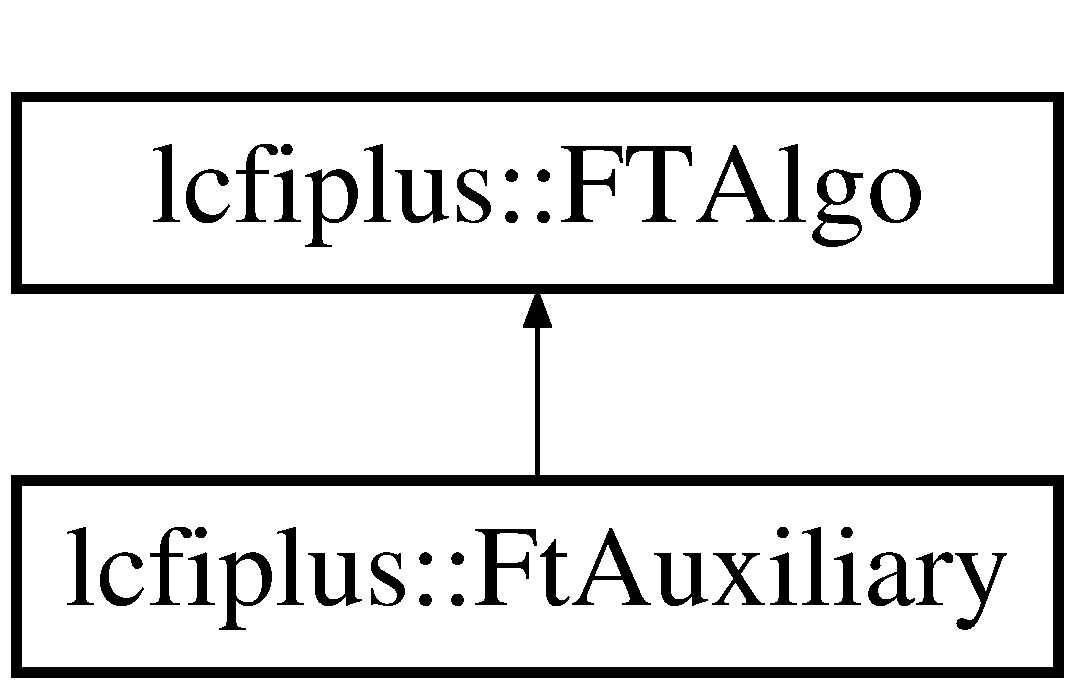
\includegraphics[height=2.000000cm]{classlcfiplus_1_1FtAuxiliary}
\end{center}
\end{figure}
\subsection*{Public Member Functions}
\begin{DoxyCompactItemize}
\item 
{\bf Ft\-Auxiliary} (const char $\ast$auxname, int auxval)
\item 
void {\bf process} ()
\end{DoxyCompactItemize}
\subsection*{Additional Inherited Members}


\subsection{Constructor \& Destructor Documentation}
\index{lcfiplus\-::\-Ft\-Auxiliary@{lcfiplus\-::\-Ft\-Auxiliary}!Ft\-Auxiliary@{Ft\-Auxiliary}}
\index{Ft\-Auxiliary@{Ft\-Auxiliary}!lcfiplus::FtAuxiliary@{lcfiplus\-::\-Ft\-Auxiliary}}
\subsubsection[{Ft\-Auxiliary}]{\setlength{\rightskip}{0pt plus 5cm}lcfiplus\-::\-Ft\-Auxiliary\-::\-Ft\-Auxiliary (
\begin{DoxyParamCaption}
\item[{const char $\ast$}]{auxname, }
\item[{int}]{auxval}
\end{DoxyParamCaption}
)\hspace{0.3cm}{\ttfamily [inline]}}\label{classlcfiplus_1_1FtAuxiliary_ad29ce89189c60cf5b80043cc21e2aebf}


\subsection{Member Function Documentation}
\index{lcfiplus\-::\-Ft\-Auxiliary@{lcfiplus\-::\-Ft\-Auxiliary}!process@{process}}
\index{process@{process}!lcfiplus::FtAuxiliary@{lcfiplus\-::\-Ft\-Auxiliary}}
\subsubsection[{process}]{\setlength{\rightskip}{0pt plus 5cm}void lcfiplus\-::\-Ft\-Auxiliary\-::process (
\begin{DoxyParamCaption}
{}
\end{DoxyParamCaption}
)\hspace{0.3cm}{\ttfamily [inline]}, {\ttfamily [virtual]}}\label{classlcfiplus_1_1FtAuxiliary_aafb10984a9f3e5d054ea7601ea23477c}


Reimplemented from {\bf lcfiplus\-::\-F\-T\-Algo} \doxyref{}{p.}{classlcfiplus_1_1FTAlgo_a23cc3f3cd1c100ab6b5e16056112351a}.



The documentation for this class was generated from the following file\-:\begin{DoxyCompactItemize}
\item 
{\bf Flavor\-Tag.\-cc}\end{DoxyCompactItemize}

\section{lcfiplus\-:\-:Ft\-Auxiliary\-M Class Reference}
\label{classlcfiplus_1_1FtAuxiliaryM}\index{lcfiplus\-::\-Ft\-Auxiliary\-M@{lcfiplus\-::\-Ft\-Auxiliary\-M}}
Inheritance diagram for lcfiplus\-:\-:Ft\-Auxiliary\-M\-:\begin{figure}[H]
\begin{center}
\leavevmode
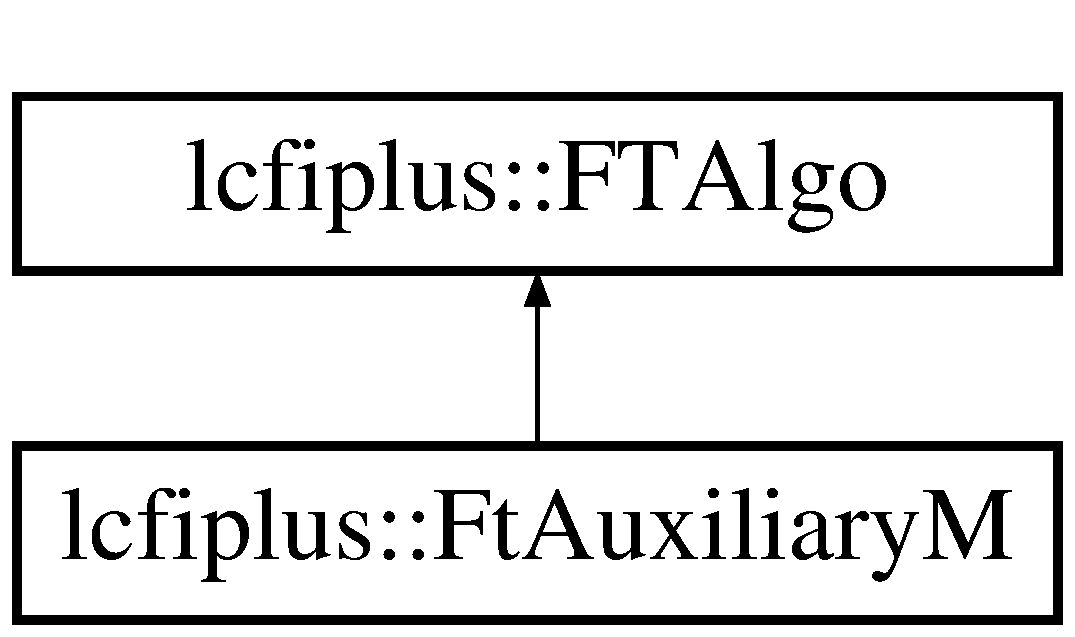
\includegraphics[height=2.000000cm]{classlcfiplus_1_1FtAuxiliaryM}
\end{center}
\end{figure}
\subsection*{Public Member Functions}
\begin{DoxyCompactItemize}
\item 
{\bf Ft\-Auxiliary\-M} (const char $\ast$auxname)
\item 
void {\bf process} ()
\end{DoxyCompactItemize}
\subsection*{Additional Inherited Members}


\subsection{Constructor \& Destructor Documentation}
\index{lcfiplus\-::\-Ft\-Auxiliary\-M@{lcfiplus\-::\-Ft\-Auxiliary\-M}!Ft\-Auxiliary\-M@{Ft\-Auxiliary\-M}}
\index{Ft\-Auxiliary\-M@{Ft\-Auxiliary\-M}!lcfiplus::FtAuxiliaryM@{lcfiplus\-::\-Ft\-Auxiliary\-M}}
\subsubsection[{Ft\-Auxiliary\-M}]{\setlength{\rightskip}{0pt plus 5cm}lcfiplus\-::\-Ft\-Auxiliary\-M\-::\-Ft\-Auxiliary\-M (
\begin{DoxyParamCaption}
\item[{const char $\ast$}]{auxname}
\end{DoxyParamCaption}
)\hspace{0.3cm}{\ttfamily [inline]}}\label{classlcfiplus_1_1FtAuxiliaryM_a478e4c75189b35a7a03c3af89b683a55}


\subsection{Member Function Documentation}
\index{lcfiplus\-::\-Ft\-Auxiliary\-M@{lcfiplus\-::\-Ft\-Auxiliary\-M}!process@{process}}
\index{process@{process}!lcfiplus::FtAuxiliaryM@{lcfiplus\-::\-Ft\-Auxiliary\-M}}
\subsubsection[{process}]{\setlength{\rightskip}{0pt plus 5cm}void lcfiplus\-::\-Ft\-Auxiliary\-M\-::process (
\begin{DoxyParamCaption}
{}
\end{DoxyParamCaption}
)\hspace{0.3cm}{\ttfamily [inline]}, {\ttfamily [virtual]}}\label{classlcfiplus_1_1FtAuxiliaryM_a2c0df248a7f26d0cdcaa7483f9829e0a}


Reimplemented from {\bf lcfiplus\-::\-F\-T\-Algo} \doxyref{}{p.}{classlcfiplus_1_1FTAlgo_a23cc3f3cd1c100ab6b5e16056112351a}.



References lcfiplus\-::\-F\-T\-Manager\-::get\-Auxiliary(), and lcfiplus\-::\-F\-T\-Manager\-::get\-Instance().



The documentation for this class was generated from the following file\-:\begin{DoxyCompactItemize}
\item 
{\bf Flavor\-Tag.\-cc}\end{DoxyCompactItemize}

\section{lcfiplus\-:\-:Ft\-B\-Ness0 Class Reference}
\label{classlcfiplus_1_1FtBNess0}\index{lcfiplus\-::\-Ft\-B\-Ness0@{lcfiplus\-::\-Ft\-B\-Ness0}}
Inheritance diagram for lcfiplus\-:\-:Ft\-B\-Ness0\-:\begin{figure}[H]
\begin{center}
\leavevmode
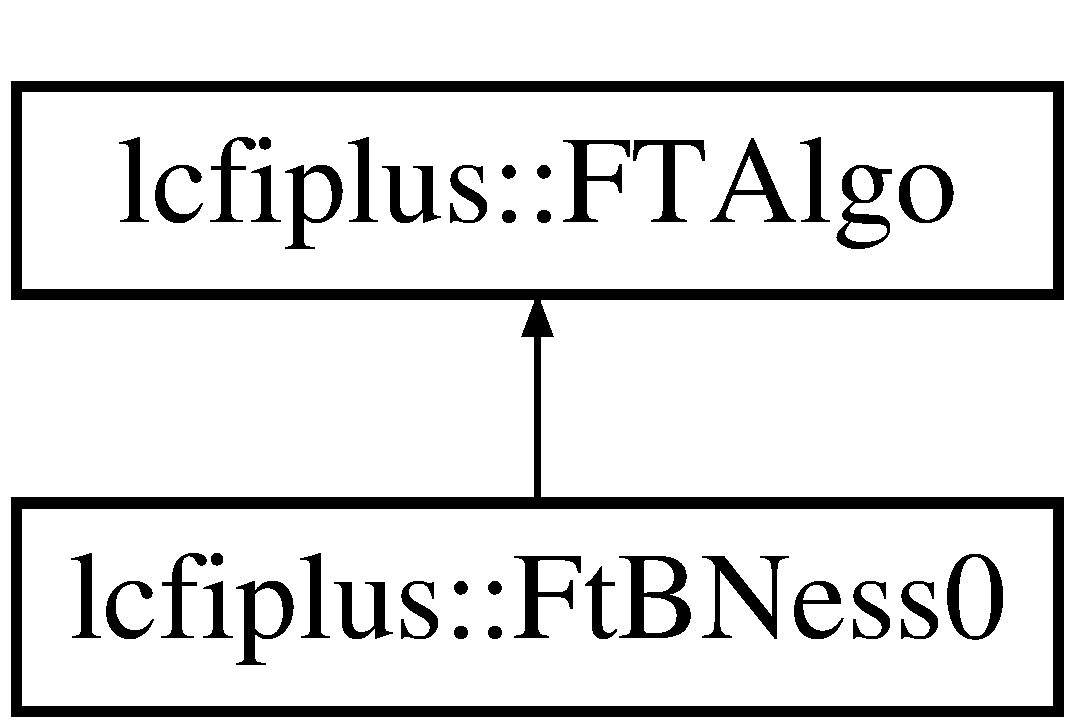
\includegraphics[height=2.000000cm]{classlcfiplus_1_1FtBNess0}
\end{center}
\end{figure}
\subsection*{Public Member Functions}
\begin{DoxyCompactItemize}
\item 
{\bf Ft\-B\-Ness0} ()
\item 
void {\bf process} ()
\end{DoxyCompactItemize}
\subsection*{Additional Inherited Members}


\subsection{Constructor \& Destructor Documentation}
\index{lcfiplus\-::\-Ft\-B\-Ness0@{lcfiplus\-::\-Ft\-B\-Ness0}!Ft\-B\-Ness0@{Ft\-B\-Ness0}}
\index{Ft\-B\-Ness0@{Ft\-B\-Ness0}!lcfiplus::FtBNess0@{lcfiplus\-::\-Ft\-B\-Ness0}}
\subsubsection[{Ft\-B\-Ness0}]{\setlength{\rightskip}{0pt plus 5cm}lcfiplus\-::\-Ft\-B\-Ness0\-::\-Ft\-B\-Ness0 (
\begin{DoxyParamCaption}
{}
\end{DoxyParamCaption}
)\hspace{0.3cm}{\ttfamily [inline]}}\label{classlcfiplus_1_1FtBNess0_acfac6ca9baa0ba428f902fd972bff8cc}


\subsection{Member Function Documentation}
\index{lcfiplus\-::\-Ft\-B\-Ness0@{lcfiplus\-::\-Ft\-B\-Ness0}!process@{process}}
\index{process@{process}!lcfiplus::FtBNess0@{lcfiplus\-::\-Ft\-B\-Ness0}}
\subsubsection[{process}]{\setlength{\rightskip}{0pt plus 5cm}void lcfiplus\-::\-Ft\-B\-Ness0\-::process (
\begin{DoxyParamCaption}
{}
\end{DoxyParamCaption}
)\hspace{0.3cm}{\ttfamily [inline]}, {\ttfamily [virtual]}}\label{classlcfiplus_1_1FtBNess0_af8d04b8f7e900520ee4057ad9d27b40f}


Reimplemented from {\bf lcfiplus\-::\-F\-T\-Algo} \doxyref{}{p.}{classlcfiplus_1_1FTAlgo_a23cc3f3cd1c100ab6b5e16056112351a}.



The documentation for this class was generated from the following file\-:\begin{DoxyCompactItemize}
\item 
{\bf Flavor\-Tag.\-cc}\end{DoxyCompactItemize}

\section{lcfiplus\-:\-:Ft\-B\-Ness1 Class Reference}
\label{classlcfiplus_1_1FtBNess1}\index{lcfiplus\-::\-Ft\-B\-Ness1@{lcfiplus\-::\-Ft\-B\-Ness1}}
Inheritance diagram for lcfiplus\-:\-:Ft\-B\-Ness1\-:\begin{figure}[H]
\begin{center}
\leavevmode
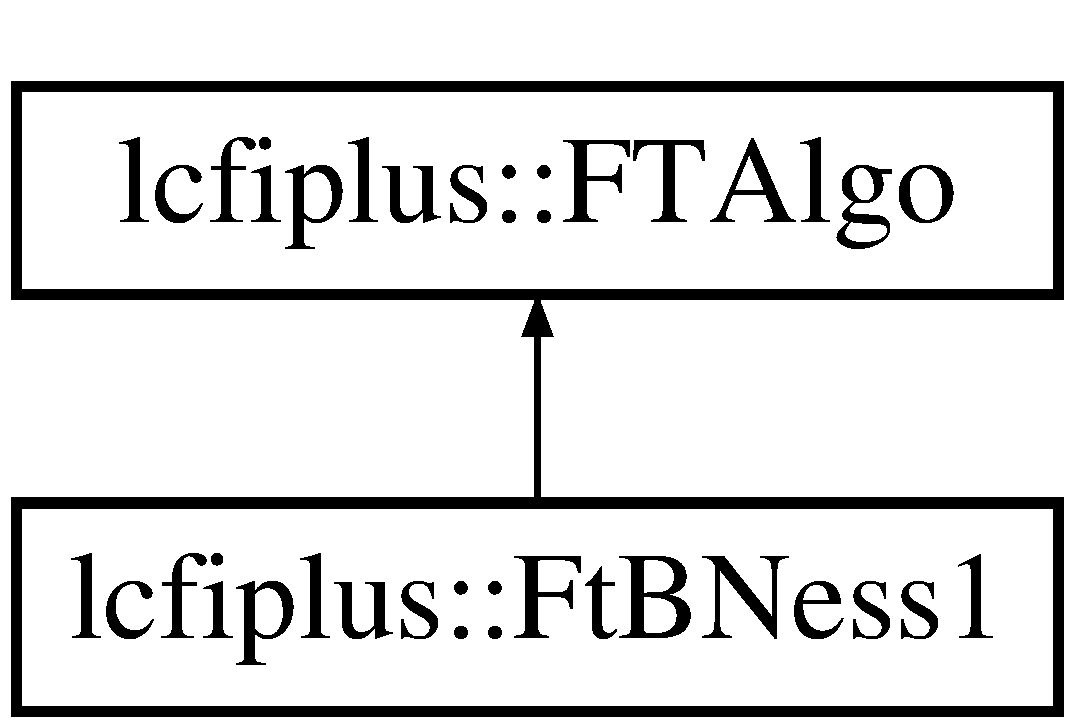
\includegraphics[height=2.000000cm]{classlcfiplus_1_1FtBNess1}
\end{center}
\end{figure}
\subsection*{Public Member Functions}
\begin{DoxyCompactItemize}
\item 
{\bf Ft\-B\-Ness1} ()
\item 
void {\bf process} ()
\end{DoxyCompactItemize}
\subsection*{Additional Inherited Members}


\subsection{Constructor \& Destructor Documentation}
\index{lcfiplus\-::\-Ft\-B\-Ness1@{lcfiplus\-::\-Ft\-B\-Ness1}!Ft\-B\-Ness1@{Ft\-B\-Ness1}}
\index{Ft\-B\-Ness1@{Ft\-B\-Ness1}!lcfiplus::FtBNess1@{lcfiplus\-::\-Ft\-B\-Ness1}}
\subsubsection[{Ft\-B\-Ness1}]{\setlength{\rightskip}{0pt plus 5cm}lcfiplus\-::\-Ft\-B\-Ness1\-::\-Ft\-B\-Ness1 (
\begin{DoxyParamCaption}
{}
\end{DoxyParamCaption}
)\hspace{0.3cm}{\ttfamily [inline]}}\label{classlcfiplus_1_1FtBNess1_a1919be68bbbe084621c6d387536a3cb2}


\subsection{Member Function Documentation}
\index{lcfiplus\-::\-Ft\-B\-Ness1@{lcfiplus\-::\-Ft\-B\-Ness1}!process@{process}}
\index{process@{process}!lcfiplus::FtBNess1@{lcfiplus\-::\-Ft\-B\-Ness1}}
\subsubsection[{process}]{\setlength{\rightskip}{0pt plus 5cm}void lcfiplus\-::\-Ft\-B\-Ness1\-::process (
\begin{DoxyParamCaption}
{}
\end{DoxyParamCaption}
)\hspace{0.3cm}{\ttfamily [inline]}, {\ttfamily [virtual]}}\label{classlcfiplus_1_1FtBNess1_a91ff1353e4e18811aece7512160fd116}


Reimplemented from {\bf lcfiplus\-::\-F\-T\-Algo} \doxyref{}{p.}{classlcfiplus_1_1FTAlgo_a23cc3f3cd1c100ab6b5e16056112351a}.



The documentation for this class was generated from the following file\-:\begin{DoxyCompactItemize}
\item 
{\bf Flavor\-Tag.\-cc}\end{DoxyCompactItemize}

\section{lcfiplus\-:\-:Ft\-B\-Ness2 Class Reference}
\label{classlcfiplus_1_1FtBNess2}\index{lcfiplus\-::\-Ft\-B\-Ness2@{lcfiplus\-::\-Ft\-B\-Ness2}}
Inheritance diagram for lcfiplus\-:\-:Ft\-B\-Ness2\-:\begin{figure}[H]
\begin{center}
\leavevmode
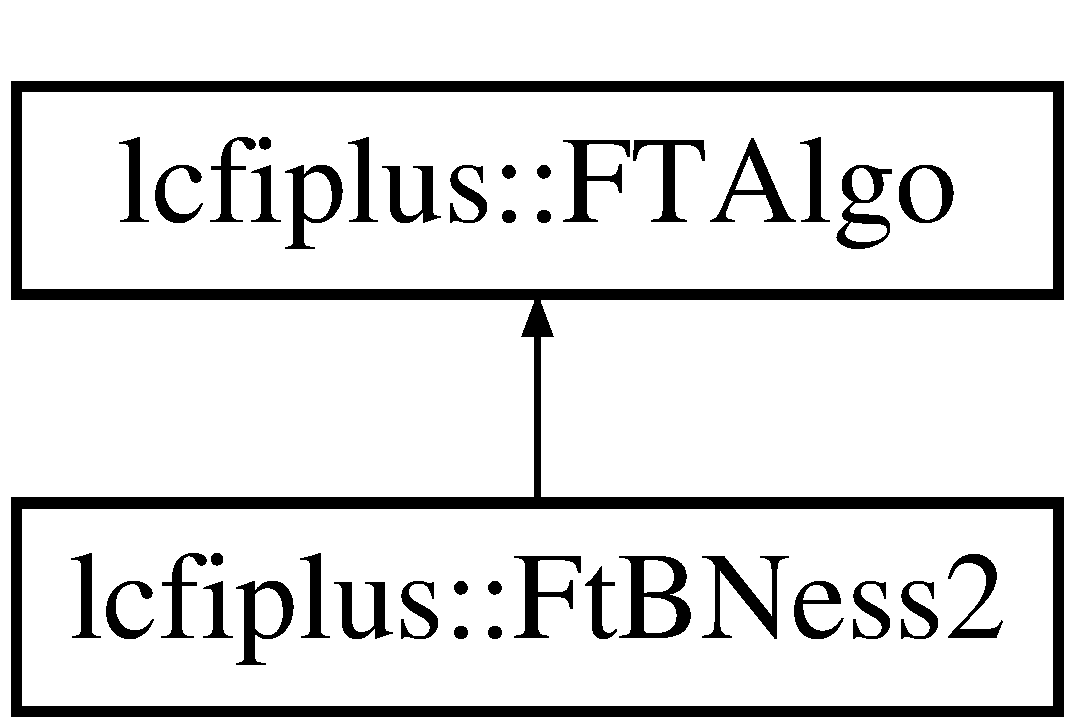
\includegraphics[height=2.000000cm]{classlcfiplus_1_1FtBNess2}
\end{center}
\end{figure}
\subsection*{Public Member Functions}
\begin{DoxyCompactItemize}
\item 
{\bf Ft\-B\-Ness2} ()
\item 
void {\bf process} ()
\end{DoxyCompactItemize}
\subsection*{Additional Inherited Members}


\subsection{Constructor \& Destructor Documentation}
\index{lcfiplus\-::\-Ft\-B\-Ness2@{lcfiplus\-::\-Ft\-B\-Ness2}!Ft\-B\-Ness2@{Ft\-B\-Ness2}}
\index{Ft\-B\-Ness2@{Ft\-B\-Ness2}!lcfiplus::FtBNess2@{lcfiplus\-::\-Ft\-B\-Ness2}}
\subsubsection[{Ft\-B\-Ness2}]{\setlength{\rightskip}{0pt plus 5cm}lcfiplus\-::\-Ft\-B\-Ness2\-::\-Ft\-B\-Ness2 (
\begin{DoxyParamCaption}
{}
\end{DoxyParamCaption}
)\hspace{0.3cm}{\ttfamily [inline]}}\label{classlcfiplus_1_1FtBNess2_a865234c66df797b918a0564e19aad423}


\subsection{Member Function Documentation}
\index{lcfiplus\-::\-Ft\-B\-Ness2@{lcfiplus\-::\-Ft\-B\-Ness2}!process@{process}}
\index{process@{process}!lcfiplus::FtBNess2@{lcfiplus\-::\-Ft\-B\-Ness2}}
\subsubsection[{process}]{\setlength{\rightskip}{0pt plus 5cm}void lcfiplus\-::\-Ft\-B\-Ness2\-::process (
\begin{DoxyParamCaption}
{}
\end{DoxyParamCaption}
)\hspace{0.3cm}{\ttfamily [inline]}, {\ttfamily [virtual]}}\label{classlcfiplus_1_1FtBNess2_a777253ce5623451441076e1f82db65d7}


Reimplemented from {\bf lcfiplus\-::\-F\-T\-Algo} \doxyref{}{p.}{classlcfiplus_1_1FTAlgo_a23cc3f3cd1c100ab6b5e16056112351a}.



The documentation for this class was generated from the following file\-:\begin{DoxyCompactItemize}
\item 
{\bf Flavor\-Tag.\-cc}\end{DoxyCompactItemize}

\section{lcfiplus\-:\-:Ft\-B\-Ness3 Class Reference}
\label{classlcfiplus_1_1FtBNess3}\index{lcfiplus\-::\-Ft\-B\-Ness3@{lcfiplus\-::\-Ft\-B\-Ness3}}
Inheritance diagram for lcfiplus\-:\-:Ft\-B\-Ness3\-:\begin{figure}[H]
\begin{center}
\leavevmode
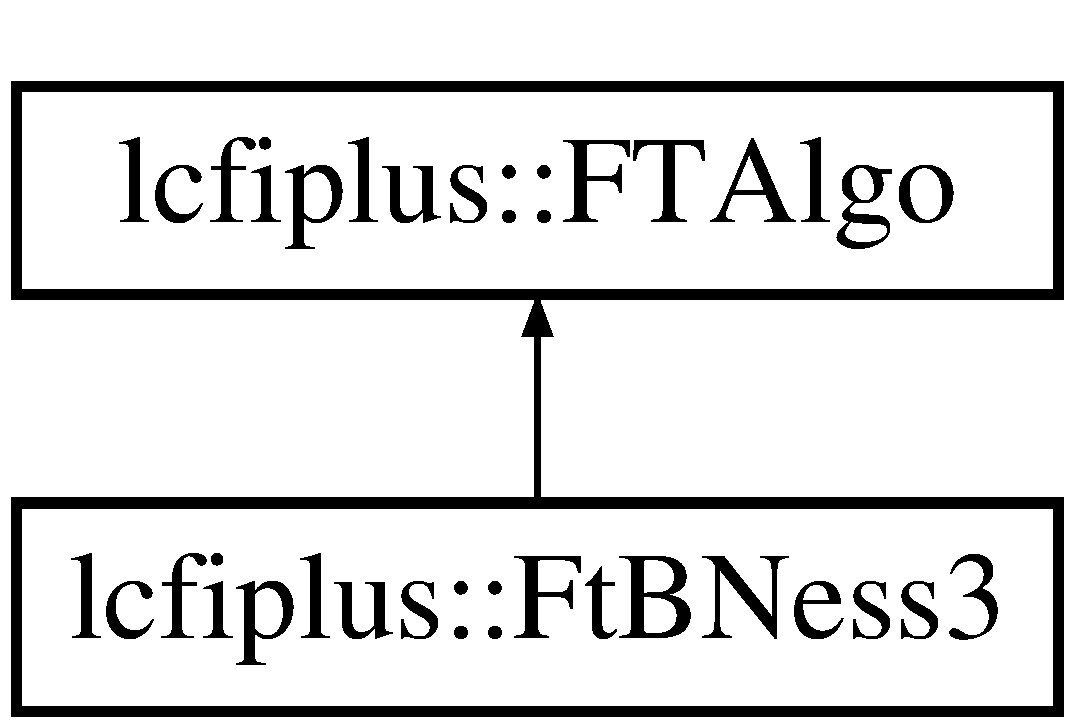
\includegraphics[height=2.000000cm]{classlcfiplus_1_1FtBNess3}
\end{center}
\end{figure}
\subsection*{Public Member Functions}
\begin{DoxyCompactItemize}
\item 
{\bf Ft\-B\-Ness3} ()
\item 
void {\bf process} ()
\end{DoxyCompactItemize}
\subsection*{Additional Inherited Members}


\subsection{Constructor \& Destructor Documentation}
\index{lcfiplus\-::\-Ft\-B\-Ness3@{lcfiplus\-::\-Ft\-B\-Ness3}!Ft\-B\-Ness3@{Ft\-B\-Ness3}}
\index{Ft\-B\-Ness3@{Ft\-B\-Ness3}!lcfiplus::FtBNess3@{lcfiplus\-::\-Ft\-B\-Ness3}}
\subsubsection[{Ft\-B\-Ness3}]{\setlength{\rightskip}{0pt plus 5cm}lcfiplus\-::\-Ft\-B\-Ness3\-::\-Ft\-B\-Ness3 (
\begin{DoxyParamCaption}
{}
\end{DoxyParamCaption}
)\hspace{0.3cm}{\ttfamily [inline]}}\label{classlcfiplus_1_1FtBNess3_aa74a35db7857c356b6b24e1d4a504ae9}


\subsection{Member Function Documentation}
\index{lcfiplus\-::\-Ft\-B\-Ness3@{lcfiplus\-::\-Ft\-B\-Ness3}!process@{process}}
\index{process@{process}!lcfiplus::FtBNess3@{lcfiplus\-::\-Ft\-B\-Ness3}}
\subsubsection[{process}]{\setlength{\rightskip}{0pt plus 5cm}void lcfiplus\-::\-Ft\-B\-Ness3\-::process (
\begin{DoxyParamCaption}
{}
\end{DoxyParamCaption}
)\hspace{0.3cm}{\ttfamily [inline]}, {\ttfamily [virtual]}}\label{classlcfiplus_1_1FtBNess3_aea7ab74de348d9897b3804d12bd4f938}


Reimplemented from {\bf lcfiplus\-::\-F\-T\-Algo} \doxyref{}{p.}{classlcfiplus_1_1FTAlgo_a23cc3f3cd1c100ab6b5e16056112351a}.



The documentation for this class was generated from the following file\-:\begin{DoxyCompactItemize}
\item 
{\bf Flavor\-Tag.\-cc}\end{DoxyCompactItemize}

\section{lcfiplus\-:\-:Ft\-B\-Ness\-Mass Class Reference}
\label{classlcfiplus_1_1FtBNessMass}\index{lcfiplus\-::\-Ft\-B\-Ness\-Mass@{lcfiplus\-::\-Ft\-B\-Ness\-Mass}}
Inheritance diagram for lcfiplus\-:\-:Ft\-B\-Ness\-Mass\-:\begin{figure}[H]
\begin{center}
\leavevmode
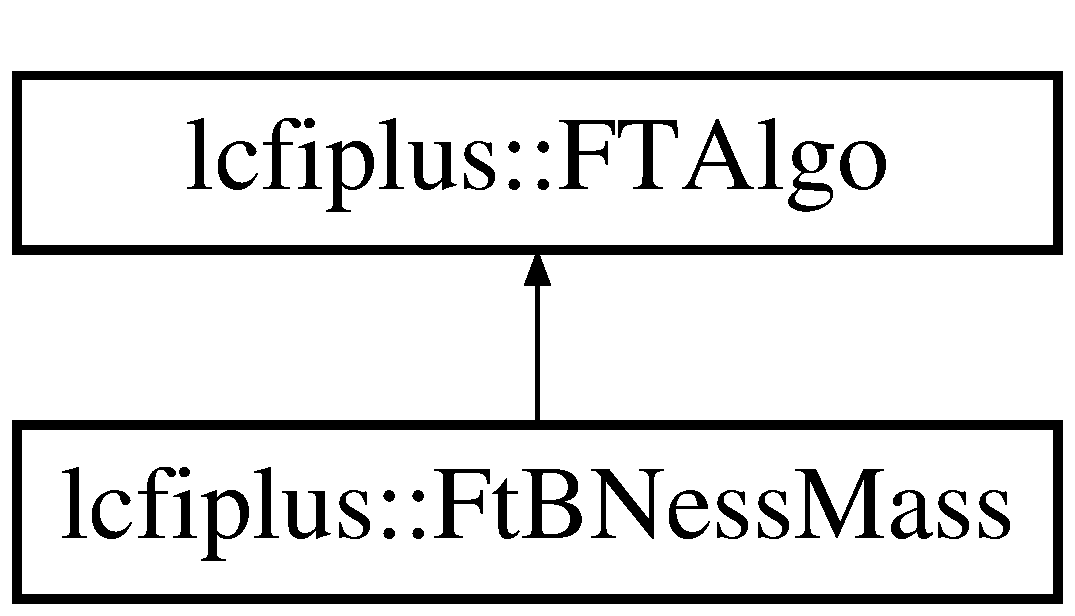
\includegraphics[height=2.000000cm]{classlcfiplus_1_1FtBNessMass}
\end{center}
\end{figure}
\subsection*{Public Member Functions}
\begin{DoxyCompactItemize}
\item 
{\bf Ft\-B\-Ness\-Mass} ()
\item 
void {\bf process} ()
\end{DoxyCompactItemize}
\subsection*{Additional Inherited Members}


\subsection{Constructor \& Destructor Documentation}
\index{lcfiplus\-::\-Ft\-B\-Ness\-Mass@{lcfiplus\-::\-Ft\-B\-Ness\-Mass}!Ft\-B\-Ness\-Mass@{Ft\-B\-Ness\-Mass}}
\index{Ft\-B\-Ness\-Mass@{Ft\-B\-Ness\-Mass}!lcfiplus::FtBNessMass@{lcfiplus\-::\-Ft\-B\-Ness\-Mass}}
\subsubsection[{Ft\-B\-Ness\-Mass}]{\setlength{\rightskip}{0pt plus 5cm}lcfiplus\-::\-Ft\-B\-Ness\-Mass\-::\-Ft\-B\-Ness\-Mass (
\begin{DoxyParamCaption}
{}
\end{DoxyParamCaption}
)\hspace{0.3cm}{\ttfamily [inline]}}\label{classlcfiplus_1_1FtBNessMass_a4fde092e92a3b8e7e5572643ea1196f6}


\subsection{Member Function Documentation}
\index{lcfiplus\-::\-Ft\-B\-Ness\-Mass@{lcfiplus\-::\-Ft\-B\-Ness\-Mass}!process@{process}}
\index{process@{process}!lcfiplus::FtBNessMass@{lcfiplus\-::\-Ft\-B\-Ness\-Mass}}
\subsubsection[{process}]{\setlength{\rightskip}{0pt plus 5cm}void lcfiplus\-::\-Ft\-B\-Ness\-Mass\-::process (
\begin{DoxyParamCaption}
{}
\end{DoxyParamCaption}
)\hspace{0.3cm}{\ttfamily [inline]}, {\ttfamily [virtual]}}\label{classlcfiplus_1_1FtBNessMass_aa542017c9cce9c344b674aae68f3084e}


Reimplemented from {\bf lcfiplus\-::\-F\-T\-Algo} \doxyref{}{p.}{classlcfiplus_1_1FTAlgo_a23cc3f3cd1c100ab6b5e16056112351a}.



The documentation for this class was generated from the following file\-:\begin{DoxyCompactItemize}
\item 
{\bf Flavor\-Tag.\-cc}\end{DoxyCompactItemize}

\section{lcfiplus\-:\-:Ft\-Corr\-Vtx\-Mass1 Class Reference}
\label{classlcfiplus_1_1FtCorrVtxMass1}\index{lcfiplus\-::\-Ft\-Corr\-Vtx\-Mass1@{lcfiplus\-::\-Ft\-Corr\-Vtx\-Mass1}}
Inheritance diagram for lcfiplus\-:\-:Ft\-Corr\-Vtx\-Mass1\-:\begin{figure}[H]
\begin{center}
\leavevmode
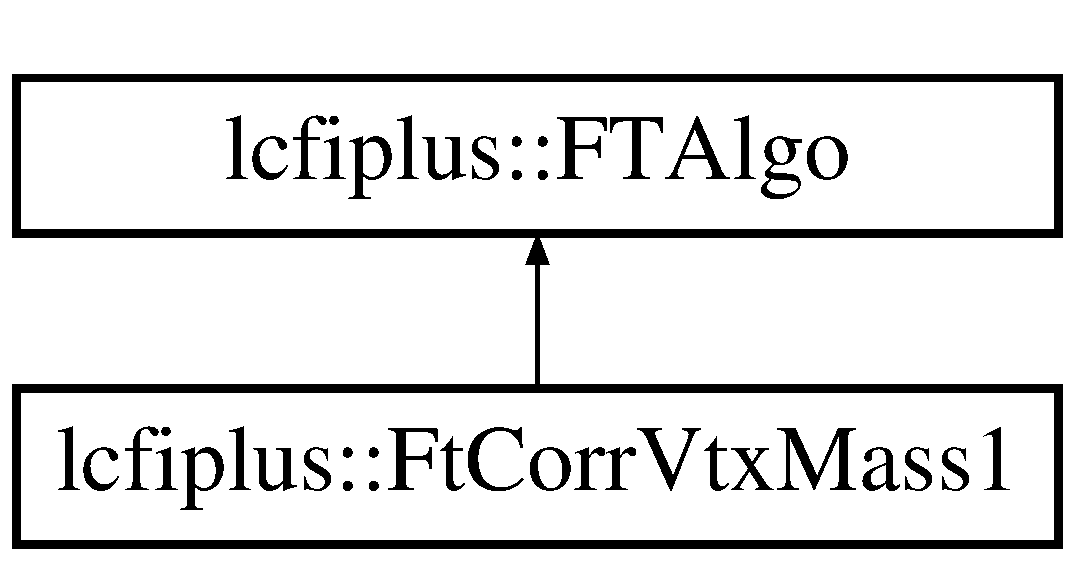
\includegraphics[height=2.000000cm]{classlcfiplus_1_1FtCorrVtxMass1}
\end{center}
\end{figure}
\subsection*{Public Member Functions}
\begin{DoxyCompactItemize}
\item 
{\bf Ft\-Corr\-Vtx\-Mass1} ()
\item 
void {\bf process} ()
\end{DoxyCompactItemize}
\subsection*{Additional Inherited Members}


\subsection{Constructor \& Destructor Documentation}
\index{lcfiplus\-::\-Ft\-Corr\-Vtx\-Mass1@{lcfiplus\-::\-Ft\-Corr\-Vtx\-Mass1}!Ft\-Corr\-Vtx\-Mass1@{Ft\-Corr\-Vtx\-Mass1}}
\index{Ft\-Corr\-Vtx\-Mass1@{Ft\-Corr\-Vtx\-Mass1}!lcfiplus::FtCorrVtxMass1@{lcfiplus\-::\-Ft\-Corr\-Vtx\-Mass1}}
\subsubsection[{Ft\-Corr\-Vtx\-Mass1}]{\setlength{\rightskip}{0pt plus 5cm}lcfiplus\-::\-Ft\-Corr\-Vtx\-Mass1\-::\-Ft\-Corr\-Vtx\-Mass1 (
\begin{DoxyParamCaption}
{}
\end{DoxyParamCaption}
)\hspace{0.3cm}{\ttfamily [inline]}}\label{classlcfiplus_1_1FtCorrVtxMass1_a108fe06d88d4c2c8b477c52844650a12}


\subsection{Member Function Documentation}
\index{lcfiplus\-::\-Ft\-Corr\-Vtx\-Mass1@{lcfiplus\-::\-Ft\-Corr\-Vtx\-Mass1}!process@{process}}
\index{process@{process}!lcfiplus::FtCorrVtxMass1@{lcfiplus\-::\-Ft\-Corr\-Vtx\-Mass1}}
\subsubsection[{process}]{\setlength{\rightskip}{0pt plus 5cm}void lcfiplus\-::\-Ft\-Corr\-Vtx\-Mass1\-::process (
\begin{DoxyParamCaption}
{}
\end{DoxyParamCaption}
)\hspace{0.3cm}{\ttfamily [inline]}, {\ttfamily [virtual]}}\label{classlcfiplus_1_1FtCorrVtxMass1_a9854c75f70d16dd4b24ef7e70a4b92dd}


Reimplemented from {\bf lcfiplus\-::\-F\-T\-Algo} \doxyref{}{p.}{classlcfiplus_1_1FTAlgo_a23cc3f3cd1c100ab6b5e16056112351a}.



The documentation for this class was generated from the following file\-:\begin{DoxyCompactItemize}
\item 
{\bf Flavor\-Tag.\-cc}\end{DoxyCompactItemize}

\section{lcfiplus\-:\-:Ft\-Corr\-Vtx\-Mass2 Class Reference}
\label{classlcfiplus_1_1FtCorrVtxMass2}\index{lcfiplus\-::\-Ft\-Corr\-Vtx\-Mass2@{lcfiplus\-::\-Ft\-Corr\-Vtx\-Mass2}}
Inheritance diagram for lcfiplus\-:\-:Ft\-Corr\-Vtx\-Mass2\-:\begin{figure}[H]
\begin{center}
\leavevmode
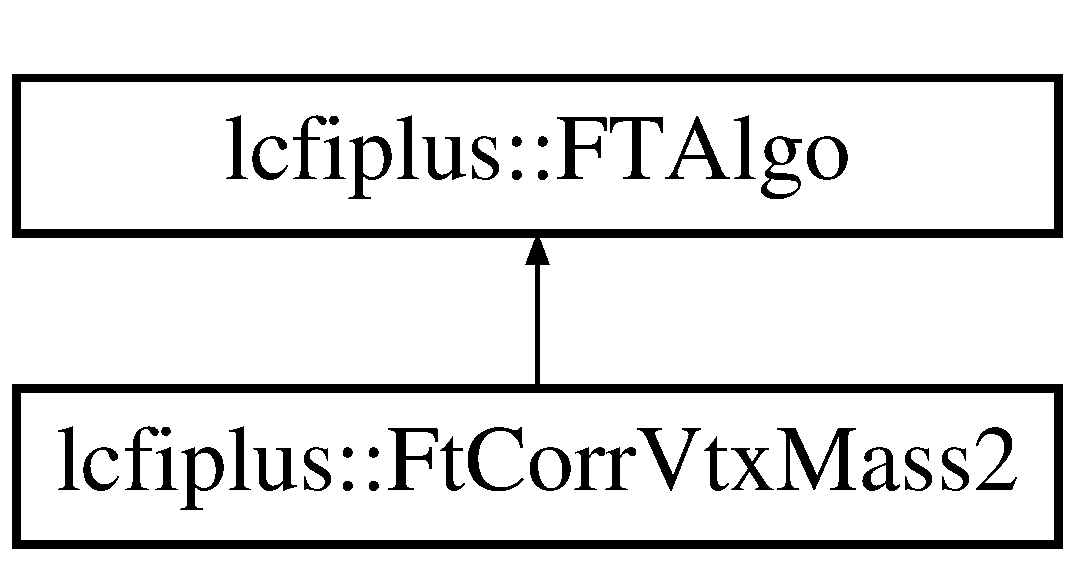
\includegraphics[height=2.000000cm]{classlcfiplus_1_1FtCorrVtxMass2}
\end{center}
\end{figure}
\subsection*{Public Member Functions}
\begin{DoxyCompactItemize}
\item 
{\bf Ft\-Corr\-Vtx\-Mass2} ()
\item 
void {\bf process} ()
\end{DoxyCompactItemize}
\subsection*{Additional Inherited Members}


\subsection{Constructor \& Destructor Documentation}
\index{lcfiplus\-::\-Ft\-Corr\-Vtx\-Mass2@{lcfiplus\-::\-Ft\-Corr\-Vtx\-Mass2}!Ft\-Corr\-Vtx\-Mass2@{Ft\-Corr\-Vtx\-Mass2}}
\index{Ft\-Corr\-Vtx\-Mass2@{Ft\-Corr\-Vtx\-Mass2}!lcfiplus::FtCorrVtxMass2@{lcfiplus\-::\-Ft\-Corr\-Vtx\-Mass2}}
\subsubsection[{Ft\-Corr\-Vtx\-Mass2}]{\setlength{\rightskip}{0pt plus 5cm}lcfiplus\-::\-Ft\-Corr\-Vtx\-Mass2\-::\-Ft\-Corr\-Vtx\-Mass2 (
\begin{DoxyParamCaption}
{}
\end{DoxyParamCaption}
)\hspace{0.3cm}{\ttfamily [inline]}}\label{classlcfiplus_1_1FtCorrVtxMass2_a11e0a5263d367f8b935411ca4e92fda4}


\subsection{Member Function Documentation}
\index{lcfiplus\-::\-Ft\-Corr\-Vtx\-Mass2@{lcfiplus\-::\-Ft\-Corr\-Vtx\-Mass2}!process@{process}}
\index{process@{process}!lcfiplus::FtCorrVtxMass2@{lcfiplus\-::\-Ft\-Corr\-Vtx\-Mass2}}
\subsubsection[{process}]{\setlength{\rightskip}{0pt plus 5cm}void lcfiplus\-::\-Ft\-Corr\-Vtx\-Mass2\-::process (
\begin{DoxyParamCaption}
{}
\end{DoxyParamCaption}
)\hspace{0.3cm}{\ttfamily [inline]}, {\ttfamily [virtual]}}\label{classlcfiplus_1_1FtCorrVtxMass2_a469cb633f5323240b29ce0779a36f1f7}


Reimplemented from {\bf lcfiplus\-::\-F\-T\-Algo} \doxyref{}{p.}{classlcfiplus_1_1FTAlgo_a23cc3f3cd1c100ab6b5e16056112351a}.



The documentation for this class was generated from the following file\-:\begin{DoxyCompactItemize}
\item 
{\bf Flavor\-Tag.\-cc}\end{DoxyCompactItemize}

\section{lcfiplus\-:\-:Ft\-Corr\-Vtx\-Mass\-All Class Reference}
\label{classlcfiplus_1_1FtCorrVtxMassAll}\index{lcfiplus\-::\-Ft\-Corr\-Vtx\-Mass\-All@{lcfiplus\-::\-Ft\-Corr\-Vtx\-Mass\-All}}
Inheritance diagram for lcfiplus\-:\-:Ft\-Corr\-Vtx\-Mass\-All\-:\begin{figure}[H]
\begin{center}
\leavevmode
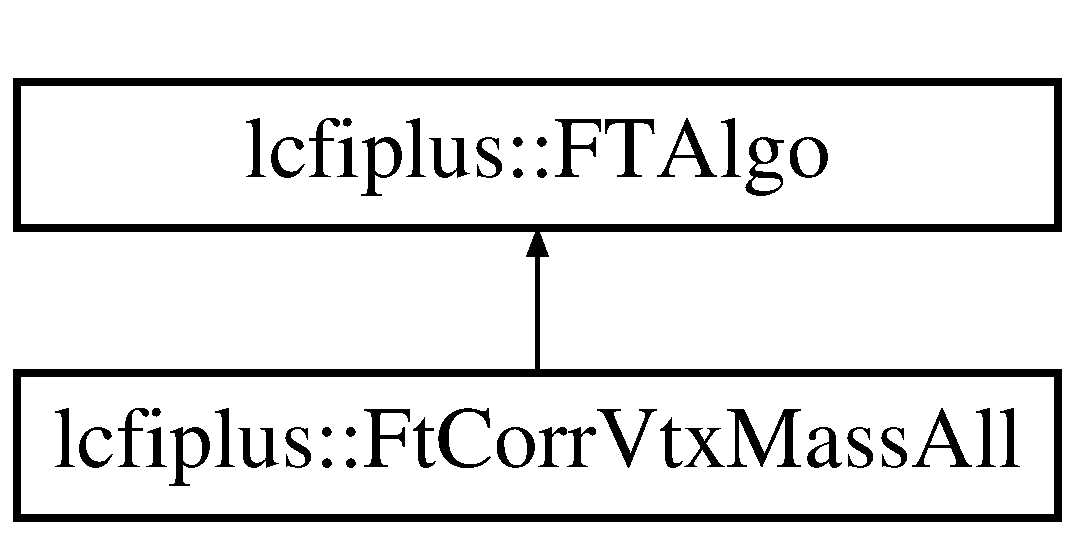
\includegraphics[height=2.000000cm]{classlcfiplus_1_1FtCorrVtxMassAll}
\end{center}
\end{figure}
\subsection*{Public Member Functions}
\begin{DoxyCompactItemize}
\item 
{\bf Ft\-Corr\-Vtx\-Mass\-All} ()
\item 
void {\bf process} ()
\end{DoxyCompactItemize}
\subsection*{Additional Inherited Members}


\subsection{Constructor \& Destructor Documentation}
\index{lcfiplus\-::\-Ft\-Corr\-Vtx\-Mass\-All@{lcfiplus\-::\-Ft\-Corr\-Vtx\-Mass\-All}!Ft\-Corr\-Vtx\-Mass\-All@{Ft\-Corr\-Vtx\-Mass\-All}}
\index{Ft\-Corr\-Vtx\-Mass\-All@{Ft\-Corr\-Vtx\-Mass\-All}!lcfiplus::FtCorrVtxMassAll@{lcfiplus\-::\-Ft\-Corr\-Vtx\-Mass\-All}}
\subsubsection[{Ft\-Corr\-Vtx\-Mass\-All}]{\setlength{\rightskip}{0pt plus 5cm}lcfiplus\-::\-Ft\-Corr\-Vtx\-Mass\-All\-::\-Ft\-Corr\-Vtx\-Mass\-All (
\begin{DoxyParamCaption}
{}
\end{DoxyParamCaption}
)\hspace{0.3cm}{\ttfamily [inline]}}\label{classlcfiplus_1_1FtCorrVtxMassAll_a2f8cb131ee0dc92148e30ec95c97f7c1}


\subsection{Member Function Documentation}
\index{lcfiplus\-::\-Ft\-Corr\-Vtx\-Mass\-All@{lcfiplus\-::\-Ft\-Corr\-Vtx\-Mass\-All}!process@{process}}
\index{process@{process}!lcfiplus::FtCorrVtxMassAll@{lcfiplus\-::\-Ft\-Corr\-Vtx\-Mass\-All}}
\subsubsection[{process}]{\setlength{\rightskip}{0pt plus 5cm}void lcfiplus\-::\-Ft\-Corr\-Vtx\-Mass\-All\-::process (
\begin{DoxyParamCaption}
{}
\end{DoxyParamCaption}
)\hspace{0.3cm}{\ttfamily [inline]}, {\ttfamily [virtual]}}\label{classlcfiplus_1_1FtCorrVtxMassAll_a2a48b21fd4d03f7c35bbe71040cec7c9}


Reimplemented from {\bf lcfiplus\-::\-F\-T\-Algo} \doxyref{}{p.}{classlcfiplus_1_1FTAlgo_a23cc3f3cd1c100ab6b5e16056112351a}.



The documentation for this class was generated from the following file\-:\begin{DoxyCompactItemize}
\item 
{\bf Flavor\-Tag.\-cc}\end{DoxyCompactItemize}

\section{lcfiplus\-:\-:Ft\-Corr\-Vtx\-Momentum1 Class Reference}
\label{classlcfiplus_1_1FtCorrVtxMomentum1}\index{lcfiplus\-::\-Ft\-Corr\-Vtx\-Momentum1@{lcfiplus\-::\-Ft\-Corr\-Vtx\-Momentum1}}
Inheritance diagram for lcfiplus\-:\-:Ft\-Corr\-Vtx\-Momentum1\-:\begin{figure}[H]
\begin{center}
\leavevmode
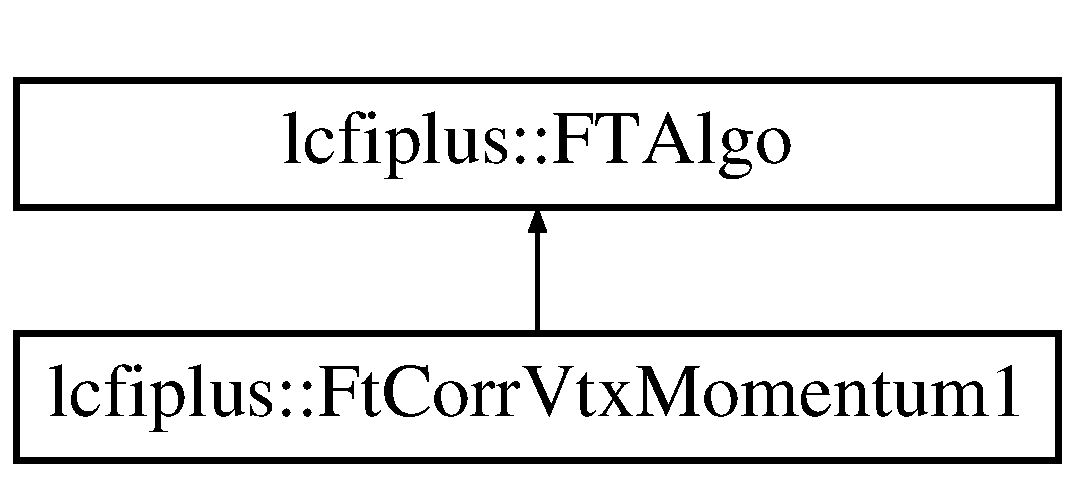
\includegraphics[height=2.000000cm]{classlcfiplus_1_1FtCorrVtxMomentum1}
\end{center}
\end{figure}
\subsection*{Public Member Functions}
\begin{DoxyCompactItemize}
\item 
{\bf Ft\-Corr\-Vtx\-Momentum1} ()
\item 
void {\bf process} ()
\end{DoxyCompactItemize}
\subsection*{Additional Inherited Members}


\subsection{Constructor \& Destructor Documentation}
\index{lcfiplus\-::\-Ft\-Corr\-Vtx\-Momentum1@{lcfiplus\-::\-Ft\-Corr\-Vtx\-Momentum1}!Ft\-Corr\-Vtx\-Momentum1@{Ft\-Corr\-Vtx\-Momentum1}}
\index{Ft\-Corr\-Vtx\-Momentum1@{Ft\-Corr\-Vtx\-Momentum1}!lcfiplus::FtCorrVtxMomentum1@{lcfiplus\-::\-Ft\-Corr\-Vtx\-Momentum1}}
\subsubsection[{Ft\-Corr\-Vtx\-Momentum1}]{\setlength{\rightskip}{0pt plus 5cm}lcfiplus\-::\-Ft\-Corr\-Vtx\-Momentum1\-::\-Ft\-Corr\-Vtx\-Momentum1 (
\begin{DoxyParamCaption}
{}
\end{DoxyParamCaption}
)\hspace{0.3cm}{\ttfamily [inline]}}\label{classlcfiplus_1_1FtCorrVtxMomentum1_a830d7cce56f862c1b9bad1279956cbe6}


\subsection{Member Function Documentation}
\index{lcfiplus\-::\-Ft\-Corr\-Vtx\-Momentum1@{lcfiplus\-::\-Ft\-Corr\-Vtx\-Momentum1}!process@{process}}
\index{process@{process}!lcfiplus::FtCorrVtxMomentum1@{lcfiplus\-::\-Ft\-Corr\-Vtx\-Momentum1}}
\subsubsection[{process}]{\setlength{\rightskip}{0pt plus 5cm}void lcfiplus\-::\-Ft\-Corr\-Vtx\-Momentum1\-::process (
\begin{DoxyParamCaption}
{}
\end{DoxyParamCaption}
)\hspace{0.3cm}{\ttfamily [inline]}, {\ttfamily [virtual]}}\label{classlcfiplus_1_1FtCorrVtxMomentum1_aed6efc62695091f145b3ee80d8d0bbc0}


Reimplemented from {\bf lcfiplus\-::\-F\-T\-Algo} \doxyref{}{p.}{classlcfiplus_1_1FTAlgo_a23cc3f3cd1c100ab6b5e16056112351a}.



The documentation for this class was generated from the following file\-:\begin{DoxyCompactItemize}
\item 
{\bf Flavor\-Tag.\-cc}\end{DoxyCompactItemize}

\section{lcfiplus\-:\-:Ft\-Corr\-Vtx\-Momentum2 Class Reference}
\label{classlcfiplus_1_1FtCorrVtxMomentum2}\index{lcfiplus\-::\-Ft\-Corr\-Vtx\-Momentum2@{lcfiplus\-::\-Ft\-Corr\-Vtx\-Momentum2}}
Inheritance diagram for lcfiplus\-:\-:Ft\-Corr\-Vtx\-Momentum2\-:\begin{figure}[H]
\begin{center}
\leavevmode
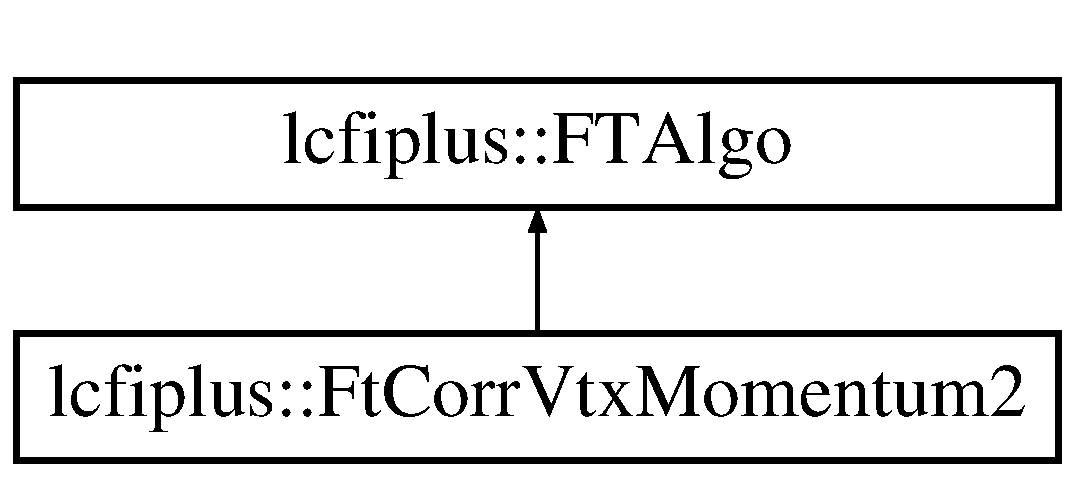
\includegraphics[height=2.000000cm]{classlcfiplus_1_1FtCorrVtxMomentum2}
\end{center}
\end{figure}
\subsection*{Public Member Functions}
\begin{DoxyCompactItemize}
\item 
{\bf Ft\-Corr\-Vtx\-Momentum2} ()
\item 
void {\bf process} ()
\end{DoxyCompactItemize}
\subsection*{Additional Inherited Members}


\subsection{Constructor \& Destructor Documentation}
\index{lcfiplus\-::\-Ft\-Corr\-Vtx\-Momentum2@{lcfiplus\-::\-Ft\-Corr\-Vtx\-Momentum2}!Ft\-Corr\-Vtx\-Momentum2@{Ft\-Corr\-Vtx\-Momentum2}}
\index{Ft\-Corr\-Vtx\-Momentum2@{Ft\-Corr\-Vtx\-Momentum2}!lcfiplus::FtCorrVtxMomentum2@{lcfiplus\-::\-Ft\-Corr\-Vtx\-Momentum2}}
\subsubsection[{Ft\-Corr\-Vtx\-Momentum2}]{\setlength{\rightskip}{0pt plus 5cm}lcfiplus\-::\-Ft\-Corr\-Vtx\-Momentum2\-::\-Ft\-Corr\-Vtx\-Momentum2 (
\begin{DoxyParamCaption}
{}
\end{DoxyParamCaption}
)\hspace{0.3cm}{\ttfamily [inline]}}\label{classlcfiplus_1_1FtCorrVtxMomentum2_aa93675795b86a694ecf41a853e503fdd}


\subsection{Member Function Documentation}
\index{lcfiplus\-::\-Ft\-Corr\-Vtx\-Momentum2@{lcfiplus\-::\-Ft\-Corr\-Vtx\-Momentum2}!process@{process}}
\index{process@{process}!lcfiplus::FtCorrVtxMomentum2@{lcfiplus\-::\-Ft\-Corr\-Vtx\-Momentum2}}
\subsubsection[{process}]{\setlength{\rightskip}{0pt plus 5cm}void lcfiplus\-::\-Ft\-Corr\-Vtx\-Momentum2\-::process (
\begin{DoxyParamCaption}
{}
\end{DoxyParamCaption}
)\hspace{0.3cm}{\ttfamily [inline]}, {\ttfamily [virtual]}}\label{classlcfiplus_1_1FtCorrVtxMomentum2_a3bbf00a47a5598287aedffbcd7f1f4e7}


Reimplemented from {\bf lcfiplus\-::\-F\-T\-Algo} \doxyref{}{p.}{classlcfiplus_1_1FTAlgo_a23cc3f3cd1c100ab6b5e16056112351a}.



The documentation for this class was generated from the following file\-:\begin{DoxyCompactItemize}
\item 
{\bf Flavor\-Tag.\-cc}\end{DoxyCompactItemize}

\section{lcfiplus\-:\-:Ft\-Corr\-Vtx\-Momentum\-All Class Reference}
\label{classlcfiplus_1_1FtCorrVtxMomentumAll}\index{lcfiplus\-::\-Ft\-Corr\-Vtx\-Momentum\-All@{lcfiplus\-::\-Ft\-Corr\-Vtx\-Momentum\-All}}
Inheritance diagram for lcfiplus\-:\-:Ft\-Corr\-Vtx\-Momentum\-All\-:\begin{figure}[H]
\begin{center}
\leavevmode
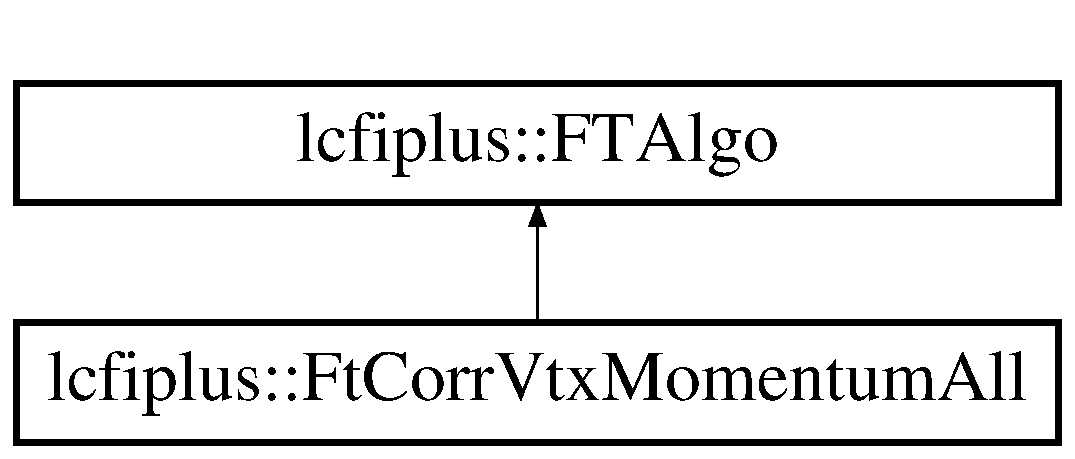
\includegraphics[height=2.000000cm]{classlcfiplus_1_1FtCorrVtxMomentumAll}
\end{center}
\end{figure}
\subsection*{Public Member Functions}
\begin{DoxyCompactItemize}
\item 
{\bf Ft\-Corr\-Vtx\-Momentum\-All} ()
\item 
void {\bf process} ()
\end{DoxyCompactItemize}
\subsection*{Additional Inherited Members}


\subsection{Constructor \& Destructor Documentation}
\index{lcfiplus\-::\-Ft\-Corr\-Vtx\-Momentum\-All@{lcfiplus\-::\-Ft\-Corr\-Vtx\-Momentum\-All}!Ft\-Corr\-Vtx\-Momentum\-All@{Ft\-Corr\-Vtx\-Momentum\-All}}
\index{Ft\-Corr\-Vtx\-Momentum\-All@{Ft\-Corr\-Vtx\-Momentum\-All}!lcfiplus::FtCorrVtxMomentumAll@{lcfiplus\-::\-Ft\-Corr\-Vtx\-Momentum\-All}}
\subsubsection[{Ft\-Corr\-Vtx\-Momentum\-All}]{\setlength{\rightskip}{0pt plus 5cm}lcfiplus\-::\-Ft\-Corr\-Vtx\-Momentum\-All\-::\-Ft\-Corr\-Vtx\-Momentum\-All (
\begin{DoxyParamCaption}
{}
\end{DoxyParamCaption}
)\hspace{0.3cm}{\ttfamily [inline]}}\label{classlcfiplus_1_1FtCorrVtxMomentumAll_a1f8959948b3bd1066ca325e598e9c06d}


\subsection{Member Function Documentation}
\index{lcfiplus\-::\-Ft\-Corr\-Vtx\-Momentum\-All@{lcfiplus\-::\-Ft\-Corr\-Vtx\-Momentum\-All}!process@{process}}
\index{process@{process}!lcfiplus::FtCorrVtxMomentumAll@{lcfiplus\-::\-Ft\-Corr\-Vtx\-Momentum\-All}}
\subsubsection[{process}]{\setlength{\rightskip}{0pt plus 5cm}void lcfiplus\-::\-Ft\-Corr\-Vtx\-Momentum\-All\-::process (
\begin{DoxyParamCaption}
{}
\end{DoxyParamCaption}
)\hspace{0.3cm}{\ttfamily [inline]}, {\ttfamily [virtual]}}\label{classlcfiplus_1_1FtCorrVtxMomentumAll_a541350ba8ec892f2d86b3072d2b5e3ad}


Reimplemented from {\bf lcfiplus\-::\-F\-T\-Algo} \doxyref{}{p.}{classlcfiplus_1_1FTAlgo_a23cc3f3cd1c100ab6b5e16056112351a}.



The documentation for this class was generated from the following file\-:\begin{DoxyCompactItemize}
\item 
{\bf Flavor\-Tag.\-cc}\end{DoxyCompactItemize}

\section{lcfiplus\-:\-:Ft\-D0b\-Prob Class Reference}
\label{classlcfiplus_1_1FtD0bProb}\index{lcfiplus\-::\-Ft\-D0b\-Prob@{lcfiplus\-::\-Ft\-D0b\-Prob}}
Inheritance diagram for lcfiplus\-:\-:Ft\-D0b\-Prob\-:\begin{figure}[H]
\begin{center}
\leavevmode
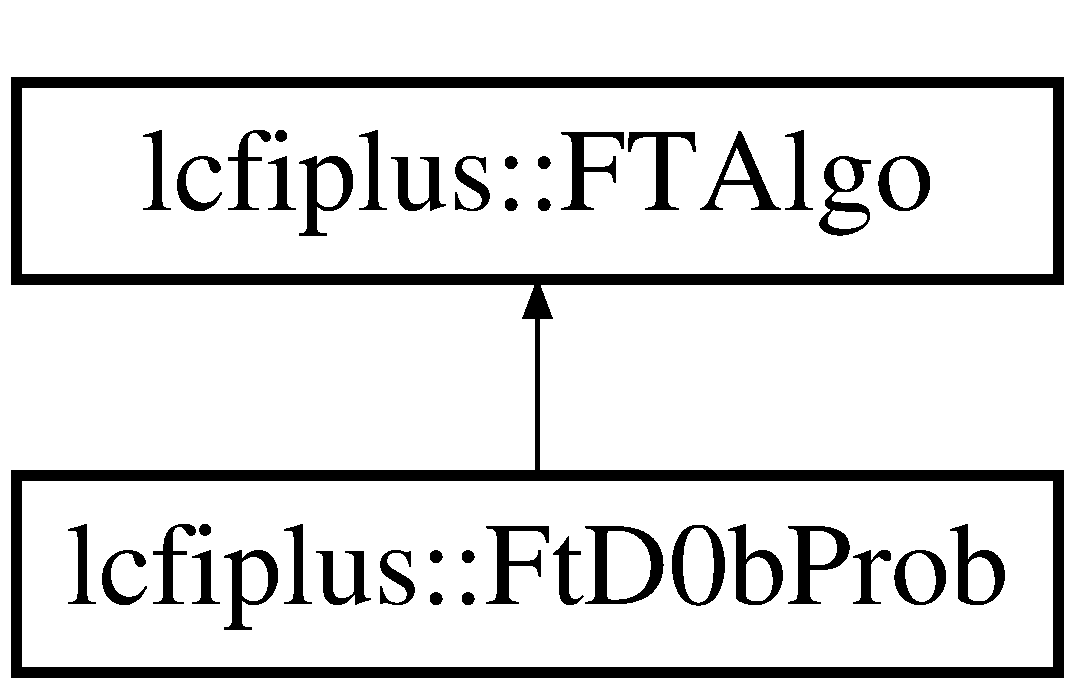
\includegraphics[height=2.000000cm]{classlcfiplus_1_1FtD0bProb}
\end{center}
\end{figure}
\subsection*{Public Member Functions}
\begin{DoxyCompactItemize}
\item 
{\bf Ft\-D0b\-Prob} ()
\item 
void {\bf process} ()
\end{DoxyCompactItemize}
\subsection*{Additional Inherited Members}


\subsection{Constructor \& Destructor Documentation}
\index{lcfiplus\-::\-Ft\-D0b\-Prob@{lcfiplus\-::\-Ft\-D0b\-Prob}!Ft\-D0b\-Prob@{Ft\-D0b\-Prob}}
\index{Ft\-D0b\-Prob@{Ft\-D0b\-Prob}!lcfiplus::FtD0bProb@{lcfiplus\-::\-Ft\-D0b\-Prob}}
\subsubsection[{Ft\-D0b\-Prob}]{\setlength{\rightskip}{0pt plus 5cm}lcfiplus\-::\-Ft\-D0b\-Prob\-::\-Ft\-D0b\-Prob (
\begin{DoxyParamCaption}
{}
\end{DoxyParamCaption}
)\hspace{0.3cm}{\ttfamily [inline]}}\label{classlcfiplus_1_1FtD0bProb_a186f503c80290b84878e12b14732c502}


\subsection{Member Function Documentation}
\index{lcfiplus\-::\-Ft\-D0b\-Prob@{lcfiplus\-::\-Ft\-D0b\-Prob}!process@{process}}
\index{process@{process}!lcfiplus::FtD0bProb@{lcfiplus\-::\-Ft\-D0b\-Prob}}
\subsubsection[{process}]{\setlength{\rightskip}{0pt plus 5cm}void lcfiplus\-::\-Ft\-D0b\-Prob\-::process (
\begin{DoxyParamCaption}
{}
\end{DoxyParamCaption}
)\hspace{0.3cm}{\ttfamily [inline]}, {\ttfamily [virtual]}}\label{classlcfiplus_1_1FtD0bProb_aa33fb90a1cb5fc5c444ea9a3317994b9}


Reimplemented from {\bf lcfiplus\-::\-F\-T\-Algo} \doxyref{}{p.}{classlcfiplus_1_1FTAlgo_a23cc3f3cd1c100ab6b5e16056112351a}.



References lcfiplus\-::\-F\-T\-Manager\-::get\-Instance(), lcfiplus\-::\-F\-T\-Manager\-::get\-I\-P\-Prob\-Holder(), and lcfiplus\-::algo\-Sig\-Prob\-::track\-D0\-Significance().



The documentation for this class was generated from the following file\-:\begin{DoxyCompactItemize}
\item 
{\bf Flavor\-Tag.\-cc}\end{DoxyCompactItemize}

\section{lcfiplus\-:\-:Ft\-D0b\-Prob2 Class Reference}
\label{classlcfiplus_1_1FtD0bProb2}\index{lcfiplus\-::\-Ft\-D0b\-Prob2@{lcfiplus\-::\-Ft\-D0b\-Prob2}}
Inheritance diagram for lcfiplus\-:\-:Ft\-D0b\-Prob2\-:\begin{figure}[H]
\begin{center}
\leavevmode
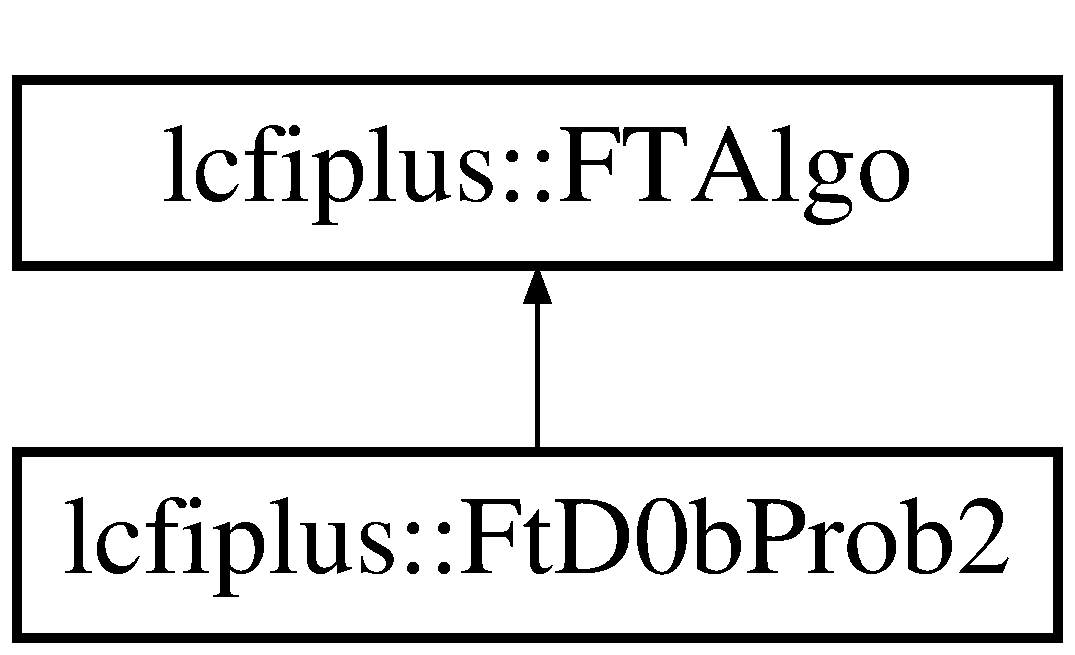
\includegraphics[height=2.000000cm]{classlcfiplus_1_1FtD0bProb2}
\end{center}
\end{figure}
\subsection*{Public Member Functions}
\begin{DoxyCompactItemize}
\item 
{\bf Ft\-D0b\-Prob2} ()
\item 
void {\bf process} ()
\end{DoxyCompactItemize}
\subsection*{Additional Inherited Members}


\subsection{Constructor \& Destructor Documentation}
\index{lcfiplus\-::\-Ft\-D0b\-Prob2@{lcfiplus\-::\-Ft\-D0b\-Prob2}!Ft\-D0b\-Prob2@{Ft\-D0b\-Prob2}}
\index{Ft\-D0b\-Prob2@{Ft\-D0b\-Prob2}!lcfiplus::FtD0bProb2@{lcfiplus\-::\-Ft\-D0b\-Prob2}}
\subsubsection[{Ft\-D0b\-Prob2}]{\setlength{\rightskip}{0pt plus 5cm}lcfiplus\-::\-Ft\-D0b\-Prob2\-::\-Ft\-D0b\-Prob2 (
\begin{DoxyParamCaption}
{}
\end{DoxyParamCaption}
)\hspace{0.3cm}{\ttfamily [inline]}}\label{classlcfiplus_1_1FtD0bProb2_a6d60b2dacff72b42e7d5df175633f3cf}


\subsection{Member Function Documentation}
\index{lcfiplus\-::\-Ft\-D0b\-Prob2@{lcfiplus\-::\-Ft\-D0b\-Prob2}!process@{process}}
\index{process@{process}!lcfiplus::FtD0bProb2@{lcfiplus\-::\-Ft\-D0b\-Prob2}}
\subsubsection[{process}]{\setlength{\rightskip}{0pt plus 5cm}void lcfiplus\-::\-Ft\-D0b\-Prob2\-::process (
\begin{DoxyParamCaption}
{}
\end{DoxyParamCaption}
)\hspace{0.3cm}{\ttfamily [inline]}, {\ttfamily [virtual]}}\label{classlcfiplus_1_1FtD0bProb2_a2b66e3cd5cfab4dfecdfbb7d76867ad7}


Reimplemented from {\bf lcfiplus\-::\-F\-T\-Algo} \doxyref{}{p.}{classlcfiplus_1_1FTAlgo_a23cc3f3cd1c100ab6b5e16056112351a}.



References lcfiplus\-::\-F\-T\-Manager\-::get\-Instance(), lcfiplus\-::\-F\-T\-Manager\-::get\-I\-P\-Prob\-Holder(), and lcfiplus\-::algo\-Sig\-Prob\-::track\-D0\-Significance().



The documentation for this class was generated from the following file\-:\begin{DoxyCompactItemize}
\item 
{\bf Flavor\-Tag.\-cc}\end{DoxyCompactItemize}

\section{lcfiplus\-:\-:Ft\-D0b\-Prob\-I\-P Class Reference}
\label{classlcfiplus_1_1FtD0bProbIP}\index{lcfiplus\-::\-Ft\-D0b\-Prob\-I\-P@{lcfiplus\-::\-Ft\-D0b\-Prob\-I\-P}}
Inheritance diagram for lcfiplus\-:\-:Ft\-D0b\-Prob\-I\-P\-:\begin{figure}[H]
\begin{center}
\leavevmode
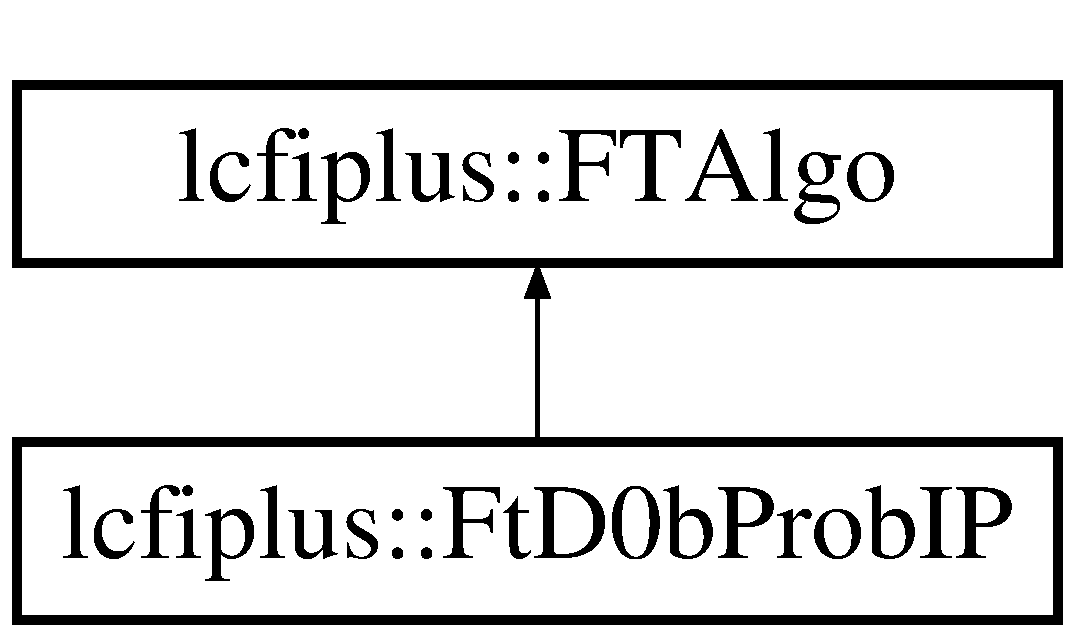
\includegraphics[height=2.000000cm]{classlcfiplus_1_1FtD0bProbIP}
\end{center}
\end{figure}
\subsection*{Public Member Functions}
\begin{DoxyCompactItemize}
\item 
{\bf Ft\-D0b\-Prob\-I\-P} ()
\item 
void {\bf process} ()
\end{DoxyCompactItemize}
\subsection*{Additional Inherited Members}


\subsection{Constructor \& Destructor Documentation}
\index{lcfiplus\-::\-Ft\-D0b\-Prob\-I\-P@{lcfiplus\-::\-Ft\-D0b\-Prob\-I\-P}!Ft\-D0b\-Prob\-I\-P@{Ft\-D0b\-Prob\-I\-P}}
\index{Ft\-D0b\-Prob\-I\-P@{Ft\-D0b\-Prob\-I\-P}!lcfiplus::FtD0bProbIP@{lcfiplus\-::\-Ft\-D0b\-Prob\-I\-P}}
\subsubsection[{Ft\-D0b\-Prob\-I\-P}]{\setlength{\rightskip}{0pt plus 5cm}lcfiplus\-::\-Ft\-D0b\-Prob\-I\-P\-::\-Ft\-D0b\-Prob\-I\-P (
\begin{DoxyParamCaption}
{}
\end{DoxyParamCaption}
)\hspace{0.3cm}{\ttfamily [inline]}}\label{classlcfiplus_1_1FtD0bProbIP_ab85ed5f8dfe00cf214f76ca6cb8df964}


\subsection{Member Function Documentation}
\index{lcfiplus\-::\-Ft\-D0b\-Prob\-I\-P@{lcfiplus\-::\-Ft\-D0b\-Prob\-I\-P}!process@{process}}
\index{process@{process}!lcfiplus::FtD0bProbIP@{lcfiplus\-::\-Ft\-D0b\-Prob\-I\-P}}
\subsubsection[{process}]{\setlength{\rightskip}{0pt plus 5cm}void lcfiplus\-::\-Ft\-D0b\-Prob\-I\-P\-::process (
\begin{DoxyParamCaption}
{}
\end{DoxyParamCaption}
)\hspace{0.3cm}{\ttfamily [inline]}, {\ttfamily [virtual]}}\label{classlcfiplus_1_1FtD0bProbIP_a8e332673a741c1134d4cb3093be77bde}


Reimplemented from {\bf lcfiplus\-::\-F\-T\-Algo} \doxyref{}{p.}{classlcfiplus_1_1FTAlgo_a23cc3f3cd1c100ab6b5e16056112351a}.



References lcfiplus\-::\-F\-T\-Manager\-::get\-Instance(), lcfiplus\-::\-F\-T\-Manager\-::get\-I\-P\-Prob\-Holder(), and lcfiplus\-::algo\-Sig\-Prob\-::signed\-D0\-Significance().



The documentation for this class was generated from the following file\-:\begin{DoxyCompactItemize}
\item 
{\bf Flavor\-Tag.\-cc}\end{DoxyCompactItemize}

\section{lcfiplus\-:\-:Ft\-D0b\-Prob\-Signed Class Reference}
\label{classlcfiplus_1_1FtD0bProbSigned}\index{lcfiplus\-::\-Ft\-D0b\-Prob\-Signed@{lcfiplus\-::\-Ft\-D0b\-Prob\-Signed}}
Inheritance diagram for lcfiplus\-:\-:Ft\-D0b\-Prob\-Signed\-:\begin{figure}[H]
\begin{center}
\leavevmode
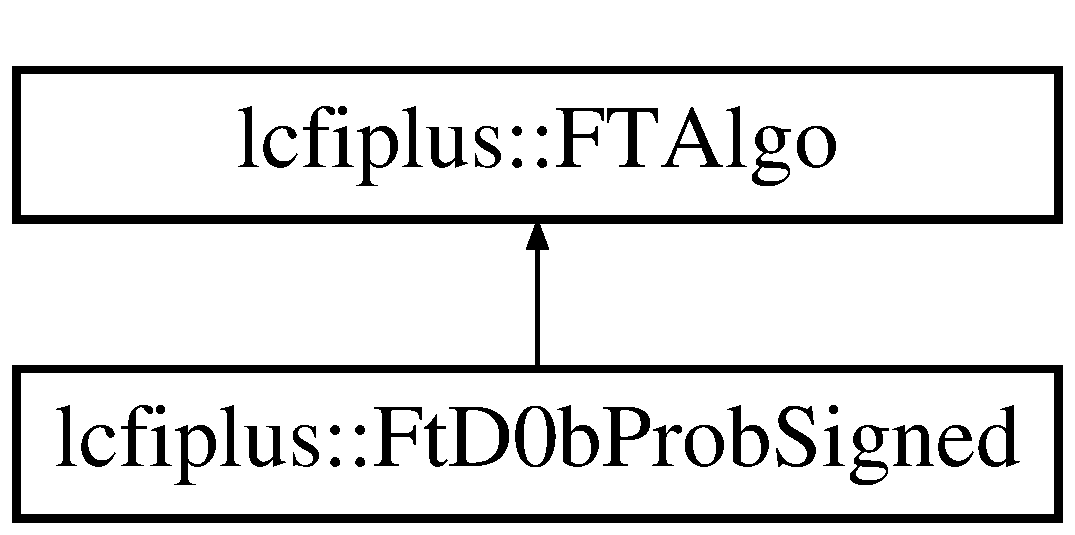
\includegraphics[height=2.000000cm]{classlcfiplus_1_1FtD0bProbSigned}
\end{center}
\end{figure}
\subsection*{Public Member Functions}
\begin{DoxyCompactItemize}
\item 
{\bf Ft\-D0b\-Prob\-Signed} (bool usevtxtracks=true)
\item 
void {\bf process} ()
\end{DoxyCompactItemize}
\subsection*{Additional Inherited Members}


\subsection{Constructor \& Destructor Documentation}
\index{lcfiplus\-::\-Ft\-D0b\-Prob\-Signed@{lcfiplus\-::\-Ft\-D0b\-Prob\-Signed}!Ft\-D0b\-Prob\-Signed@{Ft\-D0b\-Prob\-Signed}}
\index{Ft\-D0b\-Prob\-Signed@{Ft\-D0b\-Prob\-Signed}!lcfiplus::FtD0bProbSigned@{lcfiplus\-::\-Ft\-D0b\-Prob\-Signed}}
\subsubsection[{Ft\-D0b\-Prob\-Signed}]{\setlength{\rightskip}{0pt plus 5cm}lcfiplus\-::\-Ft\-D0b\-Prob\-Signed\-::\-Ft\-D0b\-Prob\-Signed (
\begin{DoxyParamCaption}
\item[{bool}]{usevtxtracks = {\ttfamily true}}
\end{DoxyParamCaption}
)\hspace{0.3cm}{\ttfamily [inline]}}\label{classlcfiplus_1_1FtD0bProbSigned_aa0e137784f6fa81464748b39677d7578}


\subsection{Member Function Documentation}
\index{lcfiplus\-::\-Ft\-D0b\-Prob\-Signed@{lcfiplus\-::\-Ft\-D0b\-Prob\-Signed}!process@{process}}
\index{process@{process}!lcfiplus::FtD0bProbSigned@{lcfiplus\-::\-Ft\-D0b\-Prob\-Signed}}
\subsubsection[{process}]{\setlength{\rightskip}{0pt plus 5cm}void lcfiplus\-::\-Ft\-D0b\-Prob\-Signed\-::process (
\begin{DoxyParamCaption}
{}
\end{DoxyParamCaption}
)\hspace{0.3cm}{\ttfamily [inline]}, {\ttfamily [virtual]}}\label{classlcfiplus_1_1FtD0bProbSigned_a575e55603f4df3743b3e2a4847355b85}


Reimplemented from {\bf lcfiplus\-::\-F\-T\-Algo} \doxyref{}{p.}{classlcfiplus_1_1FTAlgo_a23cc3f3cd1c100ab6b5e16056112351a}.



References lcfiplus\-::\-F\-T\-Manager\-::get\-Instance(), lcfiplus\-::\-F\-T\-Manager\-::get\-I\-P\-Prob\-Holder(), lcfiplus\-::algo\-Sig\-Prob\-::signed\-D0(), and lcfiplus\-::algo\-Sig\-Prob\-::track\-D0\-Significance().



The documentation for this class was generated from the following file\-:\begin{DoxyCompactItemize}
\item 
{\bf Flavor\-Tag.\-cc}\end{DoxyCompactItemize}

\section{lcfiplus\-:\-:Ft\-D0c\-Prob Class Reference}
\label{classlcfiplus_1_1FtD0cProb}\index{lcfiplus\-::\-Ft\-D0c\-Prob@{lcfiplus\-::\-Ft\-D0c\-Prob}}
Inheritance diagram for lcfiplus\-:\-:Ft\-D0c\-Prob\-:\begin{figure}[H]
\begin{center}
\leavevmode
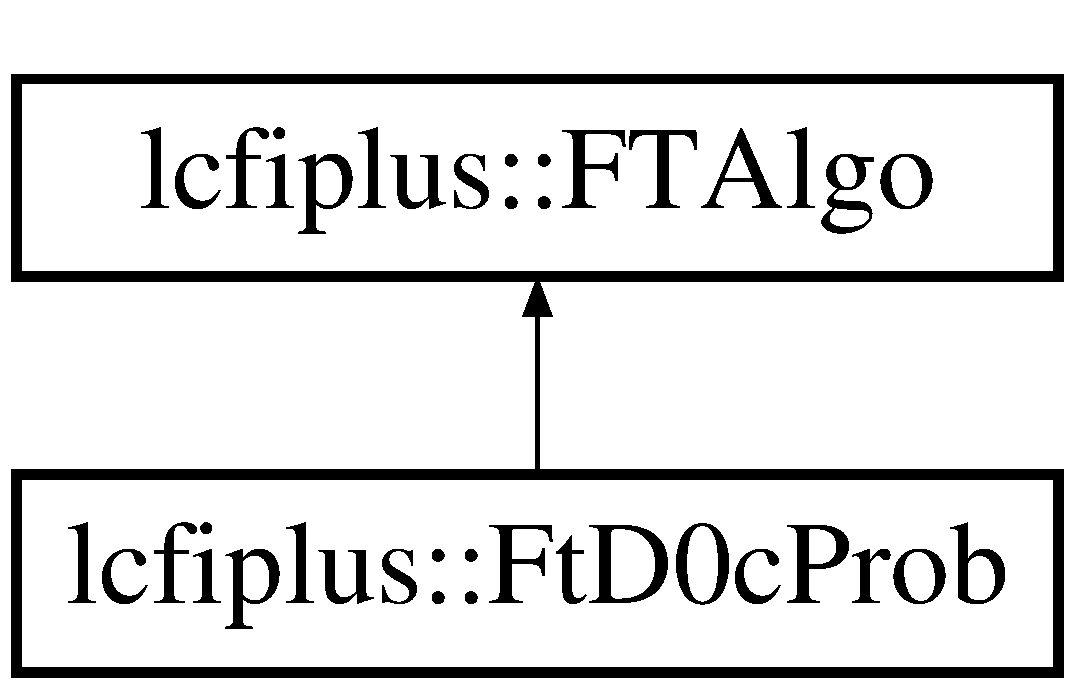
\includegraphics[height=2.000000cm]{classlcfiplus_1_1FtD0cProb}
\end{center}
\end{figure}
\subsection*{Public Member Functions}
\begin{DoxyCompactItemize}
\item 
{\bf Ft\-D0c\-Prob} ()
\item 
void {\bf process} ()
\end{DoxyCompactItemize}
\subsection*{Additional Inherited Members}


\subsection{Constructor \& Destructor Documentation}
\index{lcfiplus\-::\-Ft\-D0c\-Prob@{lcfiplus\-::\-Ft\-D0c\-Prob}!Ft\-D0c\-Prob@{Ft\-D0c\-Prob}}
\index{Ft\-D0c\-Prob@{Ft\-D0c\-Prob}!lcfiplus::FtD0cProb@{lcfiplus\-::\-Ft\-D0c\-Prob}}
\subsubsection[{Ft\-D0c\-Prob}]{\setlength{\rightskip}{0pt plus 5cm}lcfiplus\-::\-Ft\-D0c\-Prob\-::\-Ft\-D0c\-Prob (
\begin{DoxyParamCaption}
{}
\end{DoxyParamCaption}
)\hspace{0.3cm}{\ttfamily [inline]}}\label{classlcfiplus_1_1FtD0cProb_aee95b557dc19eca9074b46e7465ba98a}


\subsection{Member Function Documentation}
\index{lcfiplus\-::\-Ft\-D0c\-Prob@{lcfiplus\-::\-Ft\-D0c\-Prob}!process@{process}}
\index{process@{process}!lcfiplus::FtD0cProb@{lcfiplus\-::\-Ft\-D0c\-Prob}}
\subsubsection[{process}]{\setlength{\rightskip}{0pt plus 5cm}void lcfiplus\-::\-Ft\-D0c\-Prob\-::process (
\begin{DoxyParamCaption}
{}
\end{DoxyParamCaption}
)\hspace{0.3cm}{\ttfamily [inline]}, {\ttfamily [virtual]}}\label{classlcfiplus_1_1FtD0cProb_a3b88af3360cc9ab954541bc5e4554673}


Reimplemented from {\bf lcfiplus\-::\-F\-T\-Algo} \doxyref{}{p.}{classlcfiplus_1_1FTAlgo_a23cc3f3cd1c100ab6b5e16056112351a}.



References lcfiplus\-::\-F\-T\-Manager\-::get\-Instance(), lcfiplus\-::\-F\-T\-Manager\-::get\-I\-P\-Prob\-Holder(), and lcfiplus\-::algo\-Sig\-Prob\-::track\-D0\-Significance().



The documentation for this class was generated from the following file\-:\begin{DoxyCompactItemize}
\item 
{\bf Flavor\-Tag.\-cc}\end{DoxyCompactItemize}

\section{lcfiplus\-:\-:Ft\-D0c\-Prob2 Class Reference}
\label{classlcfiplus_1_1FtD0cProb2}\index{lcfiplus\-::\-Ft\-D0c\-Prob2@{lcfiplus\-::\-Ft\-D0c\-Prob2}}
Inheritance diagram for lcfiplus\-:\-:Ft\-D0c\-Prob2\-:\begin{figure}[H]
\begin{center}
\leavevmode
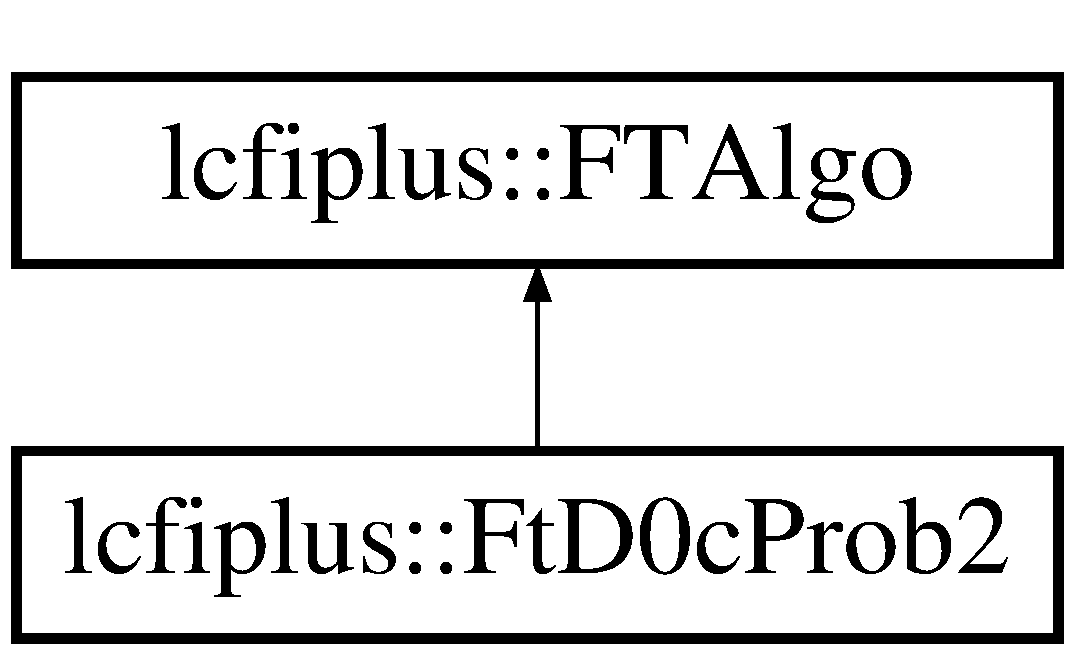
\includegraphics[height=2.000000cm]{classlcfiplus_1_1FtD0cProb2}
\end{center}
\end{figure}
\subsection*{Public Member Functions}
\begin{DoxyCompactItemize}
\item 
{\bf Ft\-D0c\-Prob2} ()
\item 
void {\bf process} ()
\end{DoxyCompactItemize}
\subsection*{Additional Inherited Members}


\subsection{Constructor \& Destructor Documentation}
\index{lcfiplus\-::\-Ft\-D0c\-Prob2@{lcfiplus\-::\-Ft\-D0c\-Prob2}!Ft\-D0c\-Prob2@{Ft\-D0c\-Prob2}}
\index{Ft\-D0c\-Prob2@{Ft\-D0c\-Prob2}!lcfiplus::FtD0cProb2@{lcfiplus\-::\-Ft\-D0c\-Prob2}}
\subsubsection[{Ft\-D0c\-Prob2}]{\setlength{\rightskip}{0pt plus 5cm}lcfiplus\-::\-Ft\-D0c\-Prob2\-::\-Ft\-D0c\-Prob2 (
\begin{DoxyParamCaption}
{}
\end{DoxyParamCaption}
)\hspace{0.3cm}{\ttfamily [inline]}}\label{classlcfiplus_1_1FtD0cProb2_af1382b7c9cafa19624102f6d6f9ea67f}


\subsection{Member Function Documentation}
\index{lcfiplus\-::\-Ft\-D0c\-Prob2@{lcfiplus\-::\-Ft\-D0c\-Prob2}!process@{process}}
\index{process@{process}!lcfiplus::FtD0cProb2@{lcfiplus\-::\-Ft\-D0c\-Prob2}}
\subsubsection[{process}]{\setlength{\rightskip}{0pt plus 5cm}void lcfiplus\-::\-Ft\-D0c\-Prob2\-::process (
\begin{DoxyParamCaption}
{}
\end{DoxyParamCaption}
)\hspace{0.3cm}{\ttfamily [inline]}, {\ttfamily [virtual]}}\label{classlcfiplus_1_1FtD0cProb2_aba032ecbae4dad88b1e1c75925134046}


Reimplemented from {\bf lcfiplus\-::\-F\-T\-Algo} \doxyref{}{p.}{classlcfiplus_1_1FTAlgo_a23cc3f3cd1c100ab6b5e16056112351a}.



References lcfiplus\-::\-F\-T\-Manager\-::get\-Instance(), lcfiplus\-::\-F\-T\-Manager\-::get\-I\-P\-Prob\-Holder(), and lcfiplus\-::algo\-Sig\-Prob\-::track\-D0\-Significance().



The documentation for this class was generated from the following file\-:\begin{DoxyCompactItemize}
\item 
{\bf Flavor\-Tag.\-cc}\end{DoxyCompactItemize}

\section{lcfiplus\-:\-:Ft\-D0c\-Prob\-I\-P Class Reference}
\label{classlcfiplus_1_1FtD0cProbIP}\index{lcfiplus\-::\-Ft\-D0c\-Prob\-I\-P@{lcfiplus\-::\-Ft\-D0c\-Prob\-I\-P}}
Inheritance diagram for lcfiplus\-:\-:Ft\-D0c\-Prob\-I\-P\-:\begin{figure}[H]
\begin{center}
\leavevmode
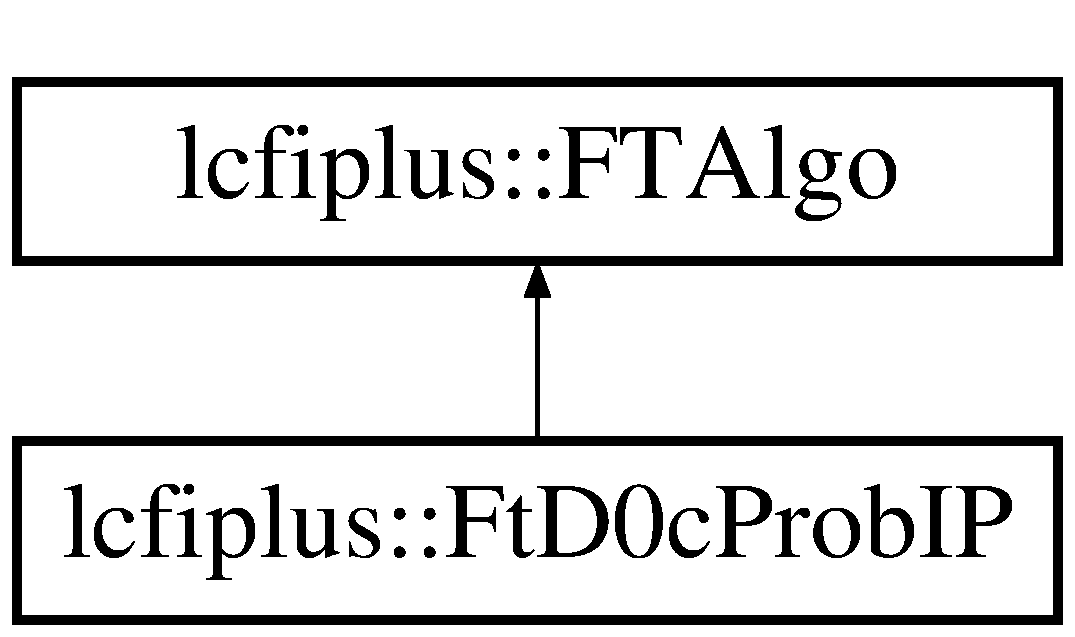
\includegraphics[height=2.000000cm]{classlcfiplus_1_1FtD0cProbIP}
\end{center}
\end{figure}
\subsection*{Public Member Functions}
\begin{DoxyCompactItemize}
\item 
{\bf Ft\-D0c\-Prob\-I\-P} ()
\item 
void {\bf process} ()
\end{DoxyCompactItemize}
\subsection*{Additional Inherited Members}


\subsection{Constructor \& Destructor Documentation}
\index{lcfiplus\-::\-Ft\-D0c\-Prob\-I\-P@{lcfiplus\-::\-Ft\-D0c\-Prob\-I\-P}!Ft\-D0c\-Prob\-I\-P@{Ft\-D0c\-Prob\-I\-P}}
\index{Ft\-D0c\-Prob\-I\-P@{Ft\-D0c\-Prob\-I\-P}!lcfiplus::FtD0cProbIP@{lcfiplus\-::\-Ft\-D0c\-Prob\-I\-P}}
\subsubsection[{Ft\-D0c\-Prob\-I\-P}]{\setlength{\rightskip}{0pt plus 5cm}lcfiplus\-::\-Ft\-D0c\-Prob\-I\-P\-::\-Ft\-D0c\-Prob\-I\-P (
\begin{DoxyParamCaption}
{}
\end{DoxyParamCaption}
)\hspace{0.3cm}{\ttfamily [inline]}}\label{classlcfiplus_1_1FtD0cProbIP_a9c84e65578029067fda1b5027d2b5807}


\subsection{Member Function Documentation}
\index{lcfiplus\-::\-Ft\-D0c\-Prob\-I\-P@{lcfiplus\-::\-Ft\-D0c\-Prob\-I\-P}!process@{process}}
\index{process@{process}!lcfiplus::FtD0cProbIP@{lcfiplus\-::\-Ft\-D0c\-Prob\-I\-P}}
\subsubsection[{process}]{\setlength{\rightskip}{0pt plus 5cm}void lcfiplus\-::\-Ft\-D0c\-Prob\-I\-P\-::process (
\begin{DoxyParamCaption}
{}
\end{DoxyParamCaption}
)\hspace{0.3cm}{\ttfamily [inline]}, {\ttfamily [virtual]}}\label{classlcfiplus_1_1FtD0cProbIP_afb0b4e7c2480d972480aae6860b0ce5a}


Reimplemented from {\bf lcfiplus\-::\-F\-T\-Algo} \doxyref{}{p.}{classlcfiplus_1_1FTAlgo_a23cc3f3cd1c100ab6b5e16056112351a}.



References lcfiplus\-::\-F\-T\-Manager\-::get\-Instance(), lcfiplus\-::\-F\-T\-Manager\-::get\-I\-P\-Prob\-Holder(), and lcfiplus\-::algo\-Sig\-Prob\-::signed\-D0\-Significance().



The documentation for this class was generated from the following file\-:\begin{DoxyCompactItemize}
\item 
{\bf Flavor\-Tag.\-cc}\end{DoxyCompactItemize}

\section{lcfiplus\-:\-:Ft\-D0c\-Prob\-Signed Class Reference}
\label{classlcfiplus_1_1FtD0cProbSigned}\index{lcfiplus\-::\-Ft\-D0c\-Prob\-Signed@{lcfiplus\-::\-Ft\-D0c\-Prob\-Signed}}
Inheritance diagram for lcfiplus\-:\-:Ft\-D0c\-Prob\-Signed\-:\begin{figure}[H]
\begin{center}
\leavevmode
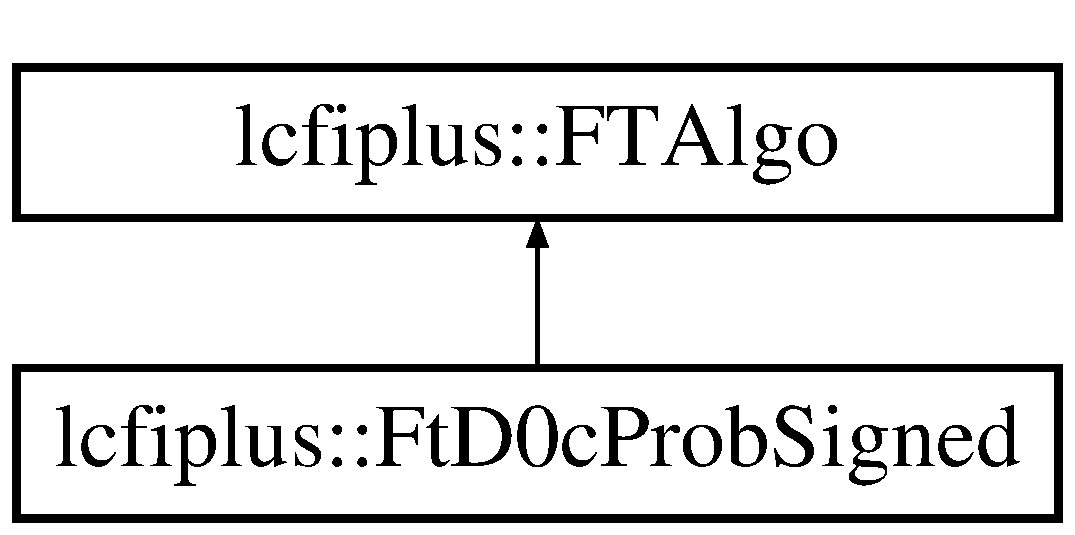
\includegraphics[height=2.000000cm]{classlcfiplus_1_1FtD0cProbSigned}
\end{center}
\end{figure}
\subsection*{Public Member Functions}
\begin{DoxyCompactItemize}
\item 
{\bf Ft\-D0c\-Prob\-Signed} (bool usevtxtracks=true)
\item 
void {\bf process} ()
\end{DoxyCompactItemize}
\subsection*{Additional Inherited Members}


\subsection{Constructor \& Destructor Documentation}
\index{lcfiplus\-::\-Ft\-D0c\-Prob\-Signed@{lcfiplus\-::\-Ft\-D0c\-Prob\-Signed}!Ft\-D0c\-Prob\-Signed@{Ft\-D0c\-Prob\-Signed}}
\index{Ft\-D0c\-Prob\-Signed@{Ft\-D0c\-Prob\-Signed}!lcfiplus::FtD0cProbSigned@{lcfiplus\-::\-Ft\-D0c\-Prob\-Signed}}
\subsubsection[{Ft\-D0c\-Prob\-Signed}]{\setlength{\rightskip}{0pt plus 5cm}lcfiplus\-::\-Ft\-D0c\-Prob\-Signed\-::\-Ft\-D0c\-Prob\-Signed (
\begin{DoxyParamCaption}
\item[{bool}]{usevtxtracks = {\ttfamily true}}
\end{DoxyParamCaption}
)\hspace{0.3cm}{\ttfamily [inline]}}\label{classlcfiplus_1_1FtD0cProbSigned_aa5740066c89877301b7b2e55e898ac3a}


\subsection{Member Function Documentation}
\index{lcfiplus\-::\-Ft\-D0c\-Prob\-Signed@{lcfiplus\-::\-Ft\-D0c\-Prob\-Signed}!process@{process}}
\index{process@{process}!lcfiplus::FtD0cProbSigned@{lcfiplus\-::\-Ft\-D0c\-Prob\-Signed}}
\subsubsection[{process}]{\setlength{\rightskip}{0pt plus 5cm}void lcfiplus\-::\-Ft\-D0c\-Prob\-Signed\-::process (
\begin{DoxyParamCaption}
{}
\end{DoxyParamCaption}
)\hspace{0.3cm}{\ttfamily [inline]}, {\ttfamily [virtual]}}\label{classlcfiplus_1_1FtD0cProbSigned_af4849ec51c395a8954ef23374a3d6e48}


Reimplemented from {\bf lcfiplus\-::\-F\-T\-Algo} \doxyref{}{p.}{classlcfiplus_1_1FTAlgo_a23cc3f3cd1c100ab6b5e16056112351a}.



References lcfiplus\-::\-F\-T\-Manager\-::get\-Instance(), lcfiplus\-::\-F\-T\-Manager\-::get\-I\-P\-Prob\-Holder(), lcfiplus\-::algo\-Sig\-Prob\-::signed\-D0(), and lcfiplus\-::algo\-Sig\-Prob\-::track\-D0\-Significance().



The documentation for this class was generated from the following file\-:\begin{DoxyCompactItemize}
\item 
{\bf Flavor\-Tag.\-cc}\end{DoxyCompactItemize}

\section{lcfiplus\-:\-:Ft\-D0q\-Prob Class Reference}
\label{classlcfiplus_1_1FtD0qProb}\index{lcfiplus\-::\-Ft\-D0q\-Prob@{lcfiplus\-::\-Ft\-D0q\-Prob}}
Inheritance diagram for lcfiplus\-:\-:Ft\-D0q\-Prob\-:\begin{figure}[H]
\begin{center}
\leavevmode
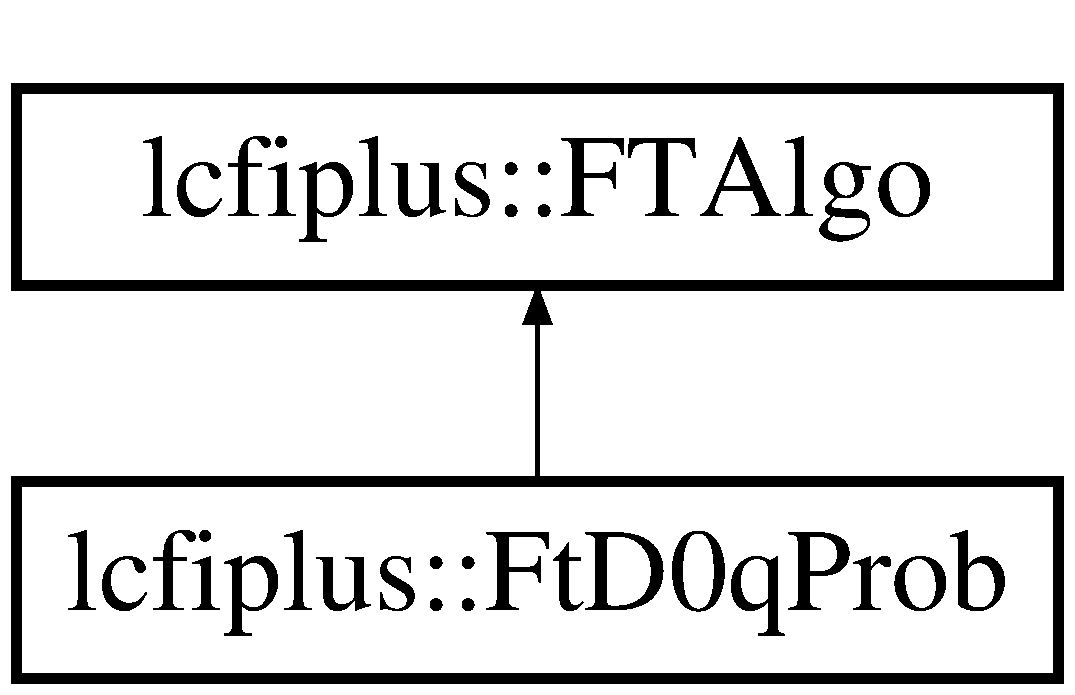
\includegraphics[height=2.000000cm]{classlcfiplus_1_1FtD0qProb}
\end{center}
\end{figure}
\subsection*{Public Member Functions}
\begin{DoxyCompactItemize}
\item 
{\bf Ft\-D0q\-Prob} ()
\item 
void {\bf process} ()
\end{DoxyCompactItemize}
\subsection*{Additional Inherited Members}


\subsection{Constructor \& Destructor Documentation}
\index{lcfiplus\-::\-Ft\-D0q\-Prob@{lcfiplus\-::\-Ft\-D0q\-Prob}!Ft\-D0q\-Prob@{Ft\-D0q\-Prob}}
\index{Ft\-D0q\-Prob@{Ft\-D0q\-Prob}!lcfiplus::FtD0qProb@{lcfiplus\-::\-Ft\-D0q\-Prob}}
\subsubsection[{Ft\-D0q\-Prob}]{\setlength{\rightskip}{0pt plus 5cm}lcfiplus\-::\-Ft\-D0q\-Prob\-::\-Ft\-D0q\-Prob (
\begin{DoxyParamCaption}
{}
\end{DoxyParamCaption}
)\hspace{0.3cm}{\ttfamily [inline]}}\label{classlcfiplus_1_1FtD0qProb_aab3043638058ebc3d2efacbbfb038dd3}


\subsection{Member Function Documentation}
\index{lcfiplus\-::\-Ft\-D0q\-Prob@{lcfiplus\-::\-Ft\-D0q\-Prob}!process@{process}}
\index{process@{process}!lcfiplus::FtD0qProb@{lcfiplus\-::\-Ft\-D0q\-Prob}}
\subsubsection[{process}]{\setlength{\rightskip}{0pt plus 5cm}void lcfiplus\-::\-Ft\-D0q\-Prob\-::process (
\begin{DoxyParamCaption}
{}
\end{DoxyParamCaption}
)\hspace{0.3cm}{\ttfamily [inline]}, {\ttfamily [virtual]}}\label{classlcfiplus_1_1FtD0qProb_a9f292cfd608518ac59b94a419f3a1f54}


Reimplemented from {\bf lcfiplus\-::\-F\-T\-Algo} \doxyref{}{p.}{classlcfiplus_1_1FTAlgo_a23cc3f3cd1c100ab6b5e16056112351a}.



References lcfiplus\-::\-F\-T\-Manager\-::get\-Instance(), lcfiplus\-::\-F\-T\-Manager\-::get\-I\-P\-Prob\-Holder(), and lcfiplus\-::algo\-Sig\-Prob\-::track\-D0\-Significance().



The documentation for this class was generated from the following file\-:\begin{DoxyCompactItemize}
\item 
{\bf Flavor\-Tag.\-cc}\end{DoxyCompactItemize}

\section{lcfiplus\-:\-:Ft\-D0q\-Prob2 Class Reference}
\label{classlcfiplus_1_1FtD0qProb2}\index{lcfiplus\-::\-Ft\-D0q\-Prob2@{lcfiplus\-::\-Ft\-D0q\-Prob2}}
Inheritance diagram for lcfiplus\-:\-:Ft\-D0q\-Prob2\-:\begin{figure}[H]
\begin{center}
\leavevmode
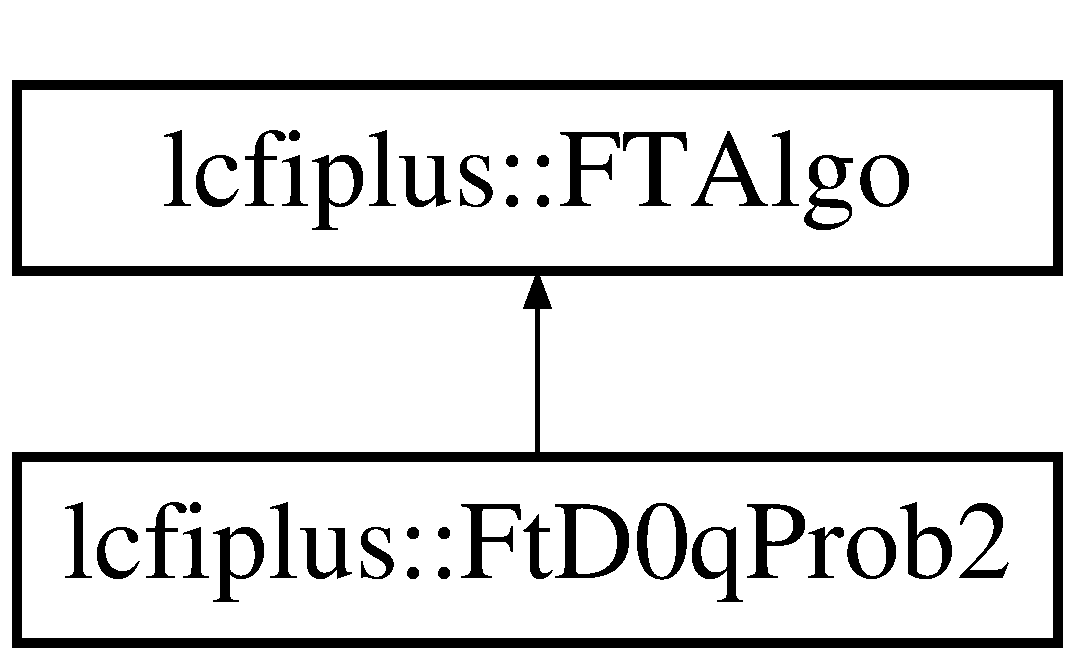
\includegraphics[height=2.000000cm]{classlcfiplus_1_1FtD0qProb2}
\end{center}
\end{figure}
\subsection*{Public Member Functions}
\begin{DoxyCompactItemize}
\item 
{\bf Ft\-D0q\-Prob2} ()
\item 
void {\bf process} ()
\end{DoxyCompactItemize}
\subsection*{Additional Inherited Members}


\subsection{Constructor \& Destructor Documentation}
\index{lcfiplus\-::\-Ft\-D0q\-Prob2@{lcfiplus\-::\-Ft\-D0q\-Prob2}!Ft\-D0q\-Prob2@{Ft\-D0q\-Prob2}}
\index{Ft\-D0q\-Prob2@{Ft\-D0q\-Prob2}!lcfiplus::FtD0qProb2@{lcfiplus\-::\-Ft\-D0q\-Prob2}}
\subsubsection[{Ft\-D0q\-Prob2}]{\setlength{\rightskip}{0pt plus 5cm}lcfiplus\-::\-Ft\-D0q\-Prob2\-::\-Ft\-D0q\-Prob2 (
\begin{DoxyParamCaption}
{}
\end{DoxyParamCaption}
)\hspace{0.3cm}{\ttfamily [inline]}}\label{classlcfiplus_1_1FtD0qProb2_a41af9ee8b9b0146e948816c2ae1bb621}


\subsection{Member Function Documentation}
\index{lcfiplus\-::\-Ft\-D0q\-Prob2@{lcfiplus\-::\-Ft\-D0q\-Prob2}!process@{process}}
\index{process@{process}!lcfiplus::FtD0qProb2@{lcfiplus\-::\-Ft\-D0q\-Prob2}}
\subsubsection[{process}]{\setlength{\rightskip}{0pt plus 5cm}void lcfiplus\-::\-Ft\-D0q\-Prob2\-::process (
\begin{DoxyParamCaption}
{}
\end{DoxyParamCaption}
)\hspace{0.3cm}{\ttfamily [inline]}, {\ttfamily [virtual]}}\label{classlcfiplus_1_1FtD0qProb2_aa393b69dfbc040f70cdae5d6edda7a1c}


Reimplemented from {\bf lcfiplus\-::\-F\-T\-Algo} \doxyref{}{p.}{classlcfiplus_1_1FTAlgo_a23cc3f3cd1c100ab6b5e16056112351a}.



References lcfiplus\-::\-F\-T\-Manager\-::get\-Instance(), lcfiplus\-::\-F\-T\-Manager\-::get\-I\-P\-Prob\-Holder(), and lcfiplus\-::algo\-Sig\-Prob\-::track\-D0\-Significance().



The documentation for this class was generated from the following file\-:\begin{DoxyCompactItemize}
\item 
{\bf Flavor\-Tag.\-cc}\end{DoxyCompactItemize}

\section{lcfiplus\-:\-:Ft\-D0q\-Prob\-Signed Class Reference}
\label{classlcfiplus_1_1FtD0qProbSigned}\index{lcfiplus\-::\-Ft\-D0q\-Prob\-Signed@{lcfiplus\-::\-Ft\-D0q\-Prob\-Signed}}
Inheritance diagram for lcfiplus\-:\-:Ft\-D0q\-Prob\-Signed\-:\begin{figure}[H]
\begin{center}
\leavevmode
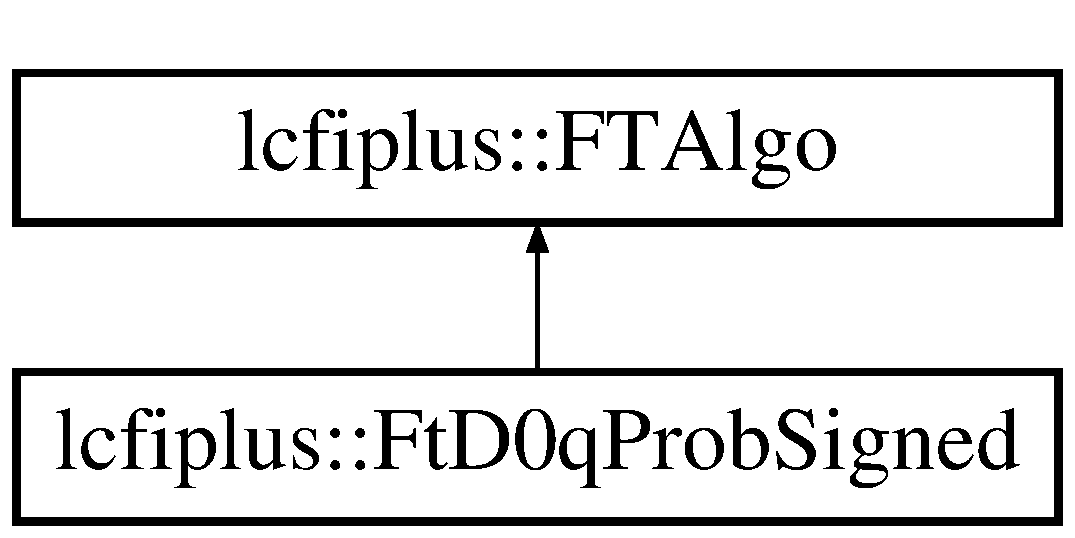
\includegraphics[height=2.000000cm]{classlcfiplus_1_1FtD0qProbSigned}
\end{center}
\end{figure}
\subsection*{Public Member Functions}
\begin{DoxyCompactItemize}
\item 
{\bf Ft\-D0q\-Prob\-Signed} (bool usevtxtracks=true)
\item 
void {\bf process} ()
\end{DoxyCompactItemize}
\subsection*{Additional Inherited Members}


\subsection{Constructor \& Destructor Documentation}
\index{lcfiplus\-::\-Ft\-D0q\-Prob\-Signed@{lcfiplus\-::\-Ft\-D0q\-Prob\-Signed}!Ft\-D0q\-Prob\-Signed@{Ft\-D0q\-Prob\-Signed}}
\index{Ft\-D0q\-Prob\-Signed@{Ft\-D0q\-Prob\-Signed}!lcfiplus::FtD0qProbSigned@{lcfiplus\-::\-Ft\-D0q\-Prob\-Signed}}
\subsubsection[{Ft\-D0q\-Prob\-Signed}]{\setlength{\rightskip}{0pt plus 5cm}lcfiplus\-::\-Ft\-D0q\-Prob\-Signed\-::\-Ft\-D0q\-Prob\-Signed (
\begin{DoxyParamCaption}
\item[{bool}]{usevtxtracks = {\ttfamily true}}
\end{DoxyParamCaption}
)\hspace{0.3cm}{\ttfamily [inline]}}\label{classlcfiplus_1_1FtD0qProbSigned_afbec7b50765214c03ccbb29108228ff6}


\subsection{Member Function Documentation}
\index{lcfiplus\-::\-Ft\-D0q\-Prob\-Signed@{lcfiplus\-::\-Ft\-D0q\-Prob\-Signed}!process@{process}}
\index{process@{process}!lcfiplus::FtD0qProbSigned@{lcfiplus\-::\-Ft\-D0q\-Prob\-Signed}}
\subsubsection[{process}]{\setlength{\rightskip}{0pt plus 5cm}void lcfiplus\-::\-Ft\-D0q\-Prob\-Signed\-::process (
\begin{DoxyParamCaption}
{}
\end{DoxyParamCaption}
)\hspace{0.3cm}{\ttfamily [inline]}, {\ttfamily [virtual]}}\label{classlcfiplus_1_1FtD0qProbSigned_a14df76a1cc006604864aca8617e2b9d2}


Reimplemented from {\bf lcfiplus\-::\-F\-T\-Algo} \doxyref{}{p.}{classlcfiplus_1_1FTAlgo_a23cc3f3cd1c100ab6b5e16056112351a}.



References lcfiplus\-::\-F\-T\-Manager\-::get\-Instance(), lcfiplus\-::\-F\-T\-Manager\-::get\-I\-P\-Prob\-Holder(), lcfiplus\-::algo\-Sig\-Prob\-::signed\-D0(), and lcfiplus\-::algo\-Sig\-Prob\-::track\-D0\-Significance().



The documentation for this class was generated from the following file\-:\begin{DoxyCompactItemize}
\item 
{\bf Flavor\-Tag.\-cc}\end{DoxyCompactItemize}

\section{lcfiplus\-:\-:Ft\-I\-P\-Prob\-Holder Class Reference}
\label{classlcfiplus_1_1FtIPProbHolder}\index{lcfiplus\-::\-Ft\-I\-P\-Prob\-Holder@{lcfiplus\-::\-Ft\-I\-P\-Prob\-Holder}}


{\ttfamily \#include $<$flavtag.\-h$>$}

\subsection*{Public Member Functions}
\begin{DoxyCompactItemize}
\item 
{\bf Ft\-I\-P\-Prob\-Holder} (const char $\ast$d0probfile, const char $\ast$z0probfile)
\item 
{\bf $\sim$\-Ft\-I\-P\-Prob\-Holder} ()
\end{DoxyCompactItemize}
\subsection*{Friends}
\begin{DoxyCompactItemize}
\item 
class {\bf Ft\-D0b\-Prob}
\item 
class {\bf Ft\-D0c\-Prob}
\item 
class {\bf Ft\-D0q\-Prob}
\item 
class {\bf Ft\-D0b\-Prob\-Signed}
\item 
class {\bf Ft\-D0c\-Prob\-Signed}
\item 
class {\bf Ft\-D0q\-Prob\-Signed}
\item 
class {\bf Ft\-D0b\-Prob\-I\-P}
\item 
class {\bf Ft\-D0c\-Prob\-I\-P}
\item 
class {\bf Ft\-Z0b\-Prob}
\item 
class {\bf Ft\-Z0c\-Prob}
\item 
class {\bf Ft\-Z0q\-Prob}
\item 
class {\bf Ft\-Z0b\-Prob\-I\-P}
\item 
class {\bf Ft\-Z0c\-Prob\-I\-P}
\item 
class {\bf Ft\-J\-Prob\-R2}
\item 
class {\bf Ft\-J\-Prob\-Z2}
\item 
class {\bf Ft\-J\-Prob\-R25\-Sigma}
\item 
class {\bf Ft\-J\-Prob\-Z25\-Sigma}
\item 
class {\bf Ft\-D0b\-Prob2}
\item 
class {\bf Ft\-D0c\-Prob2}
\item 
class {\bf Ft\-D0q\-Prob2}
\item 
class {\bf Ft\-Z0b\-Prob2}
\item 
class {\bf Ft\-Z0c\-Prob2}
\item 
class {\bf Ft\-Z0q\-Prob2}
\end{DoxyCompactItemize}


\subsection{Constructor \& Destructor Documentation}
\index{lcfiplus\-::\-Ft\-I\-P\-Prob\-Holder@{lcfiplus\-::\-Ft\-I\-P\-Prob\-Holder}!Ft\-I\-P\-Prob\-Holder@{Ft\-I\-P\-Prob\-Holder}}
\index{Ft\-I\-P\-Prob\-Holder@{Ft\-I\-P\-Prob\-Holder}!lcfiplus::FtIPProbHolder@{lcfiplus\-::\-Ft\-I\-P\-Prob\-Holder}}
\subsubsection[{Ft\-I\-P\-Prob\-Holder}]{\setlength{\rightskip}{0pt plus 5cm}lcfiplus\-::\-Ft\-I\-P\-Prob\-Holder\-::\-Ft\-I\-P\-Prob\-Holder (
\begin{DoxyParamCaption}
\item[{const char $\ast$}]{d0probfile, }
\item[{const char $\ast$}]{z0probfile}
\end{DoxyParamCaption}
)}\label{classlcfiplus_1_1FtIPProbHolder_a2cf2d8590d49a51ad725637992263967}
\index{lcfiplus\-::\-Ft\-I\-P\-Prob\-Holder@{lcfiplus\-::\-Ft\-I\-P\-Prob\-Holder}!$\sim$\-Ft\-I\-P\-Prob\-Holder@{$\sim$\-Ft\-I\-P\-Prob\-Holder}}
\index{$\sim$\-Ft\-I\-P\-Prob\-Holder@{$\sim$\-Ft\-I\-P\-Prob\-Holder}!lcfiplus::FtIPProbHolder@{lcfiplus\-::\-Ft\-I\-P\-Prob\-Holder}}
\subsubsection[{$\sim$\-Ft\-I\-P\-Prob\-Holder}]{\setlength{\rightskip}{0pt plus 5cm}lcfiplus\-::\-Ft\-I\-P\-Prob\-Holder\-::$\sim$\-Ft\-I\-P\-Prob\-Holder (
\begin{DoxyParamCaption}
{}
\end{DoxyParamCaption}
)}\label{classlcfiplus_1_1FtIPProbHolder_a96c6fd0a0a784e8e68b667ebeb7435e5}


\subsection{Friends And Related Function Documentation}
\index{lcfiplus\-::\-Ft\-I\-P\-Prob\-Holder@{lcfiplus\-::\-Ft\-I\-P\-Prob\-Holder}!Ft\-D0b\-Prob@{Ft\-D0b\-Prob}}
\index{Ft\-D0b\-Prob@{Ft\-D0b\-Prob}!lcfiplus::FtIPProbHolder@{lcfiplus\-::\-Ft\-I\-P\-Prob\-Holder}}
\subsubsection[{Ft\-D0b\-Prob}]{\setlength{\rightskip}{0pt plus 5cm}friend class {\bf Ft\-D0b\-Prob}\hspace{0.3cm}{\ttfamily [friend]}}\label{classlcfiplus_1_1FtIPProbHolder_a00d1743a67e173cdbee230f7efcbaaae}
\index{lcfiplus\-::\-Ft\-I\-P\-Prob\-Holder@{lcfiplus\-::\-Ft\-I\-P\-Prob\-Holder}!Ft\-D0b\-Prob2@{Ft\-D0b\-Prob2}}
\index{Ft\-D0b\-Prob2@{Ft\-D0b\-Prob2}!lcfiplus::FtIPProbHolder@{lcfiplus\-::\-Ft\-I\-P\-Prob\-Holder}}
\subsubsection[{Ft\-D0b\-Prob2}]{\setlength{\rightskip}{0pt plus 5cm}friend class {\bf Ft\-D0b\-Prob2}\hspace{0.3cm}{\ttfamily [friend]}}\label{classlcfiplus_1_1FtIPProbHolder_ace71a76493fd849ac75b059b5df06158}
\index{lcfiplus\-::\-Ft\-I\-P\-Prob\-Holder@{lcfiplus\-::\-Ft\-I\-P\-Prob\-Holder}!Ft\-D0b\-Prob\-I\-P@{Ft\-D0b\-Prob\-I\-P}}
\index{Ft\-D0b\-Prob\-I\-P@{Ft\-D0b\-Prob\-I\-P}!lcfiplus::FtIPProbHolder@{lcfiplus\-::\-Ft\-I\-P\-Prob\-Holder}}
\subsubsection[{Ft\-D0b\-Prob\-I\-P}]{\setlength{\rightskip}{0pt plus 5cm}friend class {\bf Ft\-D0b\-Prob\-I\-P}\hspace{0.3cm}{\ttfamily [friend]}}\label{classlcfiplus_1_1FtIPProbHolder_aba743b3b64b8c770a89d277b73ce363b}
\index{lcfiplus\-::\-Ft\-I\-P\-Prob\-Holder@{lcfiplus\-::\-Ft\-I\-P\-Prob\-Holder}!Ft\-D0b\-Prob\-Signed@{Ft\-D0b\-Prob\-Signed}}
\index{Ft\-D0b\-Prob\-Signed@{Ft\-D0b\-Prob\-Signed}!lcfiplus::FtIPProbHolder@{lcfiplus\-::\-Ft\-I\-P\-Prob\-Holder}}
\subsubsection[{Ft\-D0b\-Prob\-Signed}]{\setlength{\rightskip}{0pt plus 5cm}friend class {\bf Ft\-D0b\-Prob\-Signed}\hspace{0.3cm}{\ttfamily [friend]}}\label{classlcfiplus_1_1FtIPProbHolder_a58483aed2a536a090d39211ce75b099d}
\index{lcfiplus\-::\-Ft\-I\-P\-Prob\-Holder@{lcfiplus\-::\-Ft\-I\-P\-Prob\-Holder}!Ft\-D0c\-Prob@{Ft\-D0c\-Prob}}
\index{Ft\-D0c\-Prob@{Ft\-D0c\-Prob}!lcfiplus::FtIPProbHolder@{lcfiplus\-::\-Ft\-I\-P\-Prob\-Holder}}
\subsubsection[{Ft\-D0c\-Prob}]{\setlength{\rightskip}{0pt plus 5cm}friend class {\bf Ft\-D0c\-Prob}\hspace{0.3cm}{\ttfamily [friend]}}\label{classlcfiplus_1_1FtIPProbHolder_a5438de59fa8ce3a13ff848afa7f13d17}
\index{lcfiplus\-::\-Ft\-I\-P\-Prob\-Holder@{lcfiplus\-::\-Ft\-I\-P\-Prob\-Holder}!Ft\-D0c\-Prob2@{Ft\-D0c\-Prob2}}
\index{Ft\-D0c\-Prob2@{Ft\-D0c\-Prob2}!lcfiplus::FtIPProbHolder@{lcfiplus\-::\-Ft\-I\-P\-Prob\-Holder}}
\subsubsection[{Ft\-D0c\-Prob2}]{\setlength{\rightskip}{0pt plus 5cm}friend class {\bf Ft\-D0c\-Prob2}\hspace{0.3cm}{\ttfamily [friend]}}\label{classlcfiplus_1_1FtIPProbHolder_a55cf74614ba85182e5e35daab24c6b2e}
\index{lcfiplus\-::\-Ft\-I\-P\-Prob\-Holder@{lcfiplus\-::\-Ft\-I\-P\-Prob\-Holder}!Ft\-D0c\-Prob\-I\-P@{Ft\-D0c\-Prob\-I\-P}}
\index{Ft\-D0c\-Prob\-I\-P@{Ft\-D0c\-Prob\-I\-P}!lcfiplus::FtIPProbHolder@{lcfiplus\-::\-Ft\-I\-P\-Prob\-Holder}}
\subsubsection[{Ft\-D0c\-Prob\-I\-P}]{\setlength{\rightskip}{0pt plus 5cm}friend class {\bf Ft\-D0c\-Prob\-I\-P}\hspace{0.3cm}{\ttfamily [friend]}}\label{classlcfiplus_1_1FtIPProbHolder_a30a3ed8966a17c2bef23761214e61727}
\index{lcfiplus\-::\-Ft\-I\-P\-Prob\-Holder@{lcfiplus\-::\-Ft\-I\-P\-Prob\-Holder}!Ft\-D0c\-Prob\-Signed@{Ft\-D0c\-Prob\-Signed}}
\index{Ft\-D0c\-Prob\-Signed@{Ft\-D0c\-Prob\-Signed}!lcfiplus::FtIPProbHolder@{lcfiplus\-::\-Ft\-I\-P\-Prob\-Holder}}
\subsubsection[{Ft\-D0c\-Prob\-Signed}]{\setlength{\rightskip}{0pt plus 5cm}friend class {\bf Ft\-D0c\-Prob\-Signed}\hspace{0.3cm}{\ttfamily [friend]}}\label{classlcfiplus_1_1FtIPProbHolder_a46c618da65fcac2b63f3c869e29839dc}
\index{lcfiplus\-::\-Ft\-I\-P\-Prob\-Holder@{lcfiplus\-::\-Ft\-I\-P\-Prob\-Holder}!Ft\-D0q\-Prob@{Ft\-D0q\-Prob}}
\index{Ft\-D0q\-Prob@{Ft\-D0q\-Prob}!lcfiplus::FtIPProbHolder@{lcfiplus\-::\-Ft\-I\-P\-Prob\-Holder}}
\subsubsection[{Ft\-D0q\-Prob}]{\setlength{\rightskip}{0pt plus 5cm}friend class {\bf Ft\-D0q\-Prob}\hspace{0.3cm}{\ttfamily [friend]}}\label{classlcfiplus_1_1FtIPProbHolder_a106ad440051cd3e51fc42ccd175ea5cc}
\index{lcfiplus\-::\-Ft\-I\-P\-Prob\-Holder@{lcfiplus\-::\-Ft\-I\-P\-Prob\-Holder}!Ft\-D0q\-Prob2@{Ft\-D0q\-Prob2}}
\index{Ft\-D0q\-Prob2@{Ft\-D0q\-Prob2}!lcfiplus::FtIPProbHolder@{lcfiplus\-::\-Ft\-I\-P\-Prob\-Holder}}
\subsubsection[{Ft\-D0q\-Prob2}]{\setlength{\rightskip}{0pt plus 5cm}friend class {\bf Ft\-D0q\-Prob2}\hspace{0.3cm}{\ttfamily [friend]}}\label{classlcfiplus_1_1FtIPProbHolder_a93ab9c53136a95453f6c1b7c77b2db73}
\index{lcfiplus\-::\-Ft\-I\-P\-Prob\-Holder@{lcfiplus\-::\-Ft\-I\-P\-Prob\-Holder}!Ft\-D0q\-Prob\-Signed@{Ft\-D0q\-Prob\-Signed}}
\index{Ft\-D0q\-Prob\-Signed@{Ft\-D0q\-Prob\-Signed}!lcfiplus::FtIPProbHolder@{lcfiplus\-::\-Ft\-I\-P\-Prob\-Holder}}
\subsubsection[{Ft\-D0q\-Prob\-Signed}]{\setlength{\rightskip}{0pt plus 5cm}friend class {\bf Ft\-D0q\-Prob\-Signed}\hspace{0.3cm}{\ttfamily [friend]}}\label{classlcfiplus_1_1FtIPProbHolder_af164a98e32ba900396f1da812d995041}
\index{lcfiplus\-::\-Ft\-I\-P\-Prob\-Holder@{lcfiplus\-::\-Ft\-I\-P\-Prob\-Holder}!Ft\-J\-Prob\-R2@{Ft\-J\-Prob\-R2}}
\index{Ft\-J\-Prob\-R2@{Ft\-J\-Prob\-R2}!lcfiplus::FtIPProbHolder@{lcfiplus\-::\-Ft\-I\-P\-Prob\-Holder}}
\subsubsection[{Ft\-J\-Prob\-R2}]{\setlength{\rightskip}{0pt plus 5cm}friend class {\bf Ft\-J\-Prob\-R2}\hspace{0.3cm}{\ttfamily [friend]}}\label{classlcfiplus_1_1FtIPProbHolder_a19d74d3fb7dbef3193b0552b380e90c9}
\index{lcfiplus\-::\-Ft\-I\-P\-Prob\-Holder@{lcfiplus\-::\-Ft\-I\-P\-Prob\-Holder}!Ft\-J\-Prob\-R25\-Sigma@{Ft\-J\-Prob\-R25\-Sigma}}
\index{Ft\-J\-Prob\-R25\-Sigma@{Ft\-J\-Prob\-R25\-Sigma}!lcfiplus::FtIPProbHolder@{lcfiplus\-::\-Ft\-I\-P\-Prob\-Holder}}
\subsubsection[{Ft\-J\-Prob\-R25\-Sigma}]{\setlength{\rightskip}{0pt plus 5cm}friend class {\bf Ft\-J\-Prob\-R25\-Sigma}\hspace{0.3cm}{\ttfamily [friend]}}\label{classlcfiplus_1_1FtIPProbHolder_a9833b77a7c9fa31ee7a1f11784766790}
\index{lcfiplus\-::\-Ft\-I\-P\-Prob\-Holder@{lcfiplus\-::\-Ft\-I\-P\-Prob\-Holder}!Ft\-J\-Prob\-Z2@{Ft\-J\-Prob\-Z2}}
\index{Ft\-J\-Prob\-Z2@{Ft\-J\-Prob\-Z2}!lcfiplus::FtIPProbHolder@{lcfiplus\-::\-Ft\-I\-P\-Prob\-Holder}}
\subsubsection[{Ft\-J\-Prob\-Z2}]{\setlength{\rightskip}{0pt plus 5cm}friend class {\bf Ft\-J\-Prob\-Z2}\hspace{0.3cm}{\ttfamily [friend]}}\label{classlcfiplus_1_1FtIPProbHolder_ad9d08d4a0600f144ae02f7fc01589b00}
\index{lcfiplus\-::\-Ft\-I\-P\-Prob\-Holder@{lcfiplus\-::\-Ft\-I\-P\-Prob\-Holder}!Ft\-J\-Prob\-Z25\-Sigma@{Ft\-J\-Prob\-Z25\-Sigma}}
\index{Ft\-J\-Prob\-Z25\-Sigma@{Ft\-J\-Prob\-Z25\-Sigma}!lcfiplus::FtIPProbHolder@{lcfiplus\-::\-Ft\-I\-P\-Prob\-Holder}}
\subsubsection[{Ft\-J\-Prob\-Z25\-Sigma}]{\setlength{\rightskip}{0pt plus 5cm}friend class {\bf Ft\-J\-Prob\-Z25\-Sigma}\hspace{0.3cm}{\ttfamily [friend]}}\label{classlcfiplus_1_1FtIPProbHolder_a4296fa6039939fcf9ddd5cf7d4c643bf}
\index{lcfiplus\-::\-Ft\-I\-P\-Prob\-Holder@{lcfiplus\-::\-Ft\-I\-P\-Prob\-Holder}!Ft\-Z0b\-Prob@{Ft\-Z0b\-Prob}}
\index{Ft\-Z0b\-Prob@{Ft\-Z0b\-Prob}!lcfiplus::FtIPProbHolder@{lcfiplus\-::\-Ft\-I\-P\-Prob\-Holder}}
\subsubsection[{Ft\-Z0b\-Prob}]{\setlength{\rightskip}{0pt plus 5cm}friend class {\bf Ft\-Z0b\-Prob}\hspace{0.3cm}{\ttfamily [friend]}}\label{classlcfiplus_1_1FtIPProbHolder_a9275e1dc2967f1daa531aab2844f4d1f}
\index{lcfiplus\-::\-Ft\-I\-P\-Prob\-Holder@{lcfiplus\-::\-Ft\-I\-P\-Prob\-Holder}!Ft\-Z0b\-Prob2@{Ft\-Z0b\-Prob2}}
\index{Ft\-Z0b\-Prob2@{Ft\-Z0b\-Prob2}!lcfiplus::FtIPProbHolder@{lcfiplus\-::\-Ft\-I\-P\-Prob\-Holder}}
\subsubsection[{Ft\-Z0b\-Prob2}]{\setlength{\rightskip}{0pt plus 5cm}friend class {\bf Ft\-Z0b\-Prob2}\hspace{0.3cm}{\ttfamily [friend]}}\label{classlcfiplus_1_1FtIPProbHolder_a8bcf1c03c8950cc0c6335191b1bd99d3}
\index{lcfiplus\-::\-Ft\-I\-P\-Prob\-Holder@{lcfiplus\-::\-Ft\-I\-P\-Prob\-Holder}!Ft\-Z0b\-Prob\-I\-P@{Ft\-Z0b\-Prob\-I\-P}}
\index{Ft\-Z0b\-Prob\-I\-P@{Ft\-Z0b\-Prob\-I\-P}!lcfiplus::FtIPProbHolder@{lcfiplus\-::\-Ft\-I\-P\-Prob\-Holder}}
\subsubsection[{Ft\-Z0b\-Prob\-I\-P}]{\setlength{\rightskip}{0pt plus 5cm}friend class {\bf Ft\-Z0b\-Prob\-I\-P}\hspace{0.3cm}{\ttfamily [friend]}}\label{classlcfiplus_1_1FtIPProbHolder_a1a05b3c399d256de6a6403add76dd22d}
\index{lcfiplus\-::\-Ft\-I\-P\-Prob\-Holder@{lcfiplus\-::\-Ft\-I\-P\-Prob\-Holder}!Ft\-Z0c\-Prob@{Ft\-Z0c\-Prob}}
\index{Ft\-Z0c\-Prob@{Ft\-Z0c\-Prob}!lcfiplus::FtIPProbHolder@{lcfiplus\-::\-Ft\-I\-P\-Prob\-Holder}}
\subsubsection[{Ft\-Z0c\-Prob}]{\setlength{\rightskip}{0pt plus 5cm}friend class {\bf Ft\-Z0c\-Prob}\hspace{0.3cm}{\ttfamily [friend]}}\label{classlcfiplus_1_1FtIPProbHolder_a815eb78f6e24e8e304f67a294b17e5bd}
\index{lcfiplus\-::\-Ft\-I\-P\-Prob\-Holder@{lcfiplus\-::\-Ft\-I\-P\-Prob\-Holder}!Ft\-Z0c\-Prob2@{Ft\-Z0c\-Prob2}}
\index{Ft\-Z0c\-Prob2@{Ft\-Z0c\-Prob2}!lcfiplus::FtIPProbHolder@{lcfiplus\-::\-Ft\-I\-P\-Prob\-Holder}}
\subsubsection[{Ft\-Z0c\-Prob2}]{\setlength{\rightskip}{0pt plus 5cm}friend class {\bf Ft\-Z0c\-Prob2}\hspace{0.3cm}{\ttfamily [friend]}}\label{classlcfiplus_1_1FtIPProbHolder_a9ead47313d24628d00eaaf771656bbaa}
\index{lcfiplus\-::\-Ft\-I\-P\-Prob\-Holder@{lcfiplus\-::\-Ft\-I\-P\-Prob\-Holder}!Ft\-Z0c\-Prob\-I\-P@{Ft\-Z0c\-Prob\-I\-P}}
\index{Ft\-Z0c\-Prob\-I\-P@{Ft\-Z0c\-Prob\-I\-P}!lcfiplus::FtIPProbHolder@{lcfiplus\-::\-Ft\-I\-P\-Prob\-Holder}}
\subsubsection[{Ft\-Z0c\-Prob\-I\-P}]{\setlength{\rightskip}{0pt plus 5cm}friend class {\bf Ft\-Z0c\-Prob\-I\-P}\hspace{0.3cm}{\ttfamily [friend]}}\label{classlcfiplus_1_1FtIPProbHolder_a843d4e920977d7eadc0c925754347867}
\index{lcfiplus\-::\-Ft\-I\-P\-Prob\-Holder@{lcfiplus\-::\-Ft\-I\-P\-Prob\-Holder}!Ft\-Z0q\-Prob@{Ft\-Z0q\-Prob}}
\index{Ft\-Z0q\-Prob@{Ft\-Z0q\-Prob}!lcfiplus::FtIPProbHolder@{lcfiplus\-::\-Ft\-I\-P\-Prob\-Holder}}
\subsubsection[{Ft\-Z0q\-Prob}]{\setlength{\rightskip}{0pt plus 5cm}friend class {\bf Ft\-Z0q\-Prob}\hspace{0.3cm}{\ttfamily [friend]}}\label{classlcfiplus_1_1FtIPProbHolder_a611b901fcff025fcb9ba65d33a8af535}
\index{lcfiplus\-::\-Ft\-I\-P\-Prob\-Holder@{lcfiplus\-::\-Ft\-I\-P\-Prob\-Holder}!Ft\-Z0q\-Prob2@{Ft\-Z0q\-Prob2}}
\index{Ft\-Z0q\-Prob2@{Ft\-Z0q\-Prob2}!lcfiplus::FtIPProbHolder@{lcfiplus\-::\-Ft\-I\-P\-Prob\-Holder}}
\subsubsection[{Ft\-Z0q\-Prob2}]{\setlength{\rightskip}{0pt plus 5cm}friend class {\bf Ft\-Z0q\-Prob2}\hspace{0.3cm}{\ttfamily [friend]}}\label{classlcfiplus_1_1FtIPProbHolder_a09544ba11cbad27359547b8644e7448d}


The documentation for this class was generated from the following files\-:\begin{DoxyCompactItemize}
\item 
{\bf flavtag.\-h}\item 
{\bf flavtag.\-cc}\end{DoxyCompactItemize}

\section{lcfiplus\-:\-:Ft\-Jet\-E Class Reference}
\label{classlcfiplus_1_1FtJetE}\index{lcfiplus\-::\-Ft\-Jet\-E@{lcfiplus\-::\-Ft\-Jet\-E}}
Inheritance diagram for lcfiplus\-:\-:Ft\-Jet\-E\-:\begin{figure}[H]
\begin{center}
\leavevmode
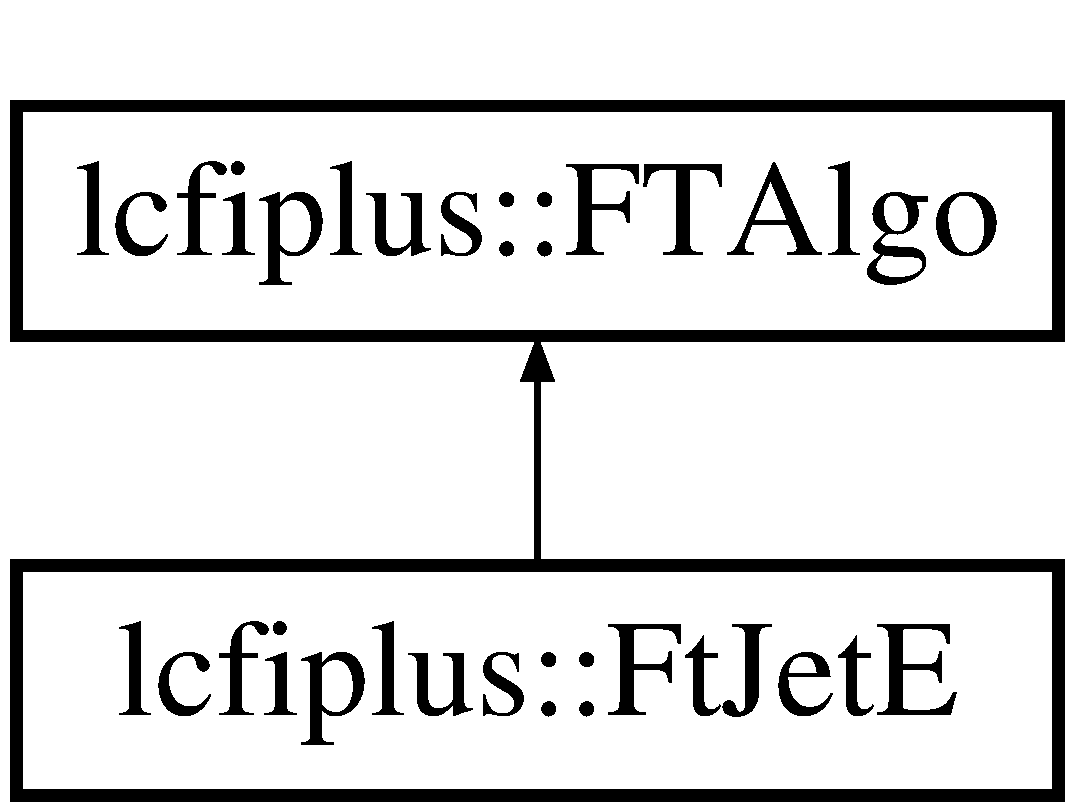
\includegraphics[height=2.000000cm]{classlcfiplus_1_1FtJetE}
\end{center}
\end{figure}
\subsection*{Public Member Functions}
\begin{DoxyCompactItemize}
\item 
{\bf Ft\-Jet\-E} ()
\item 
void {\bf process} ()
\end{DoxyCompactItemize}
\subsection*{Additional Inherited Members}


\subsection{Constructor \& Destructor Documentation}
\index{lcfiplus\-::\-Ft\-Jet\-E@{lcfiplus\-::\-Ft\-Jet\-E}!Ft\-Jet\-E@{Ft\-Jet\-E}}
\index{Ft\-Jet\-E@{Ft\-Jet\-E}!lcfiplus::FtJetE@{lcfiplus\-::\-Ft\-Jet\-E}}
\subsubsection[{Ft\-Jet\-E}]{\setlength{\rightskip}{0pt plus 5cm}lcfiplus\-::\-Ft\-Jet\-E\-::\-Ft\-Jet\-E (
\begin{DoxyParamCaption}
{}
\end{DoxyParamCaption}
)\hspace{0.3cm}{\ttfamily [inline]}}\label{classlcfiplus_1_1FtJetE_af714a98a397a00d42cc88fa5912f293f}


\subsection{Member Function Documentation}
\index{lcfiplus\-::\-Ft\-Jet\-E@{lcfiplus\-::\-Ft\-Jet\-E}!process@{process}}
\index{process@{process}!lcfiplus::FtJetE@{lcfiplus\-::\-Ft\-Jet\-E}}
\subsubsection[{process}]{\setlength{\rightskip}{0pt plus 5cm}void lcfiplus\-::\-Ft\-Jet\-E\-::process (
\begin{DoxyParamCaption}
{}
\end{DoxyParamCaption}
)\hspace{0.3cm}{\ttfamily [inline]}, {\ttfamily [virtual]}}\label{classlcfiplus_1_1FtJetE_ab39abe153f0a14a4aa5de8145d6d1e30}


Reimplemented from {\bf lcfiplus\-::\-F\-T\-Algo} \doxyref{}{p.}{classlcfiplus_1_1FTAlgo_a23cc3f3cd1c100ab6b5e16056112351a}.



The documentation for this class was generated from the following file\-:\begin{DoxyCompactItemize}
\item 
{\bf Flavor\-Tag.\-cc}\end{DoxyCompactItemize}

\section{lcfiplus\-:\-:Ft\-J\-Prob\-R Class Reference}
\label{classlcfiplus_1_1FtJProbR}\index{lcfiplus\-::\-Ft\-J\-Prob\-R@{lcfiplus\-::\-Ft\-J\-Prob\-R}}
Inheritance diagram for lcfiplus\-:\-:Ft\-J\-Prob\-R\-:\begin{figure}[H]
\begin{center}
\leavevmode
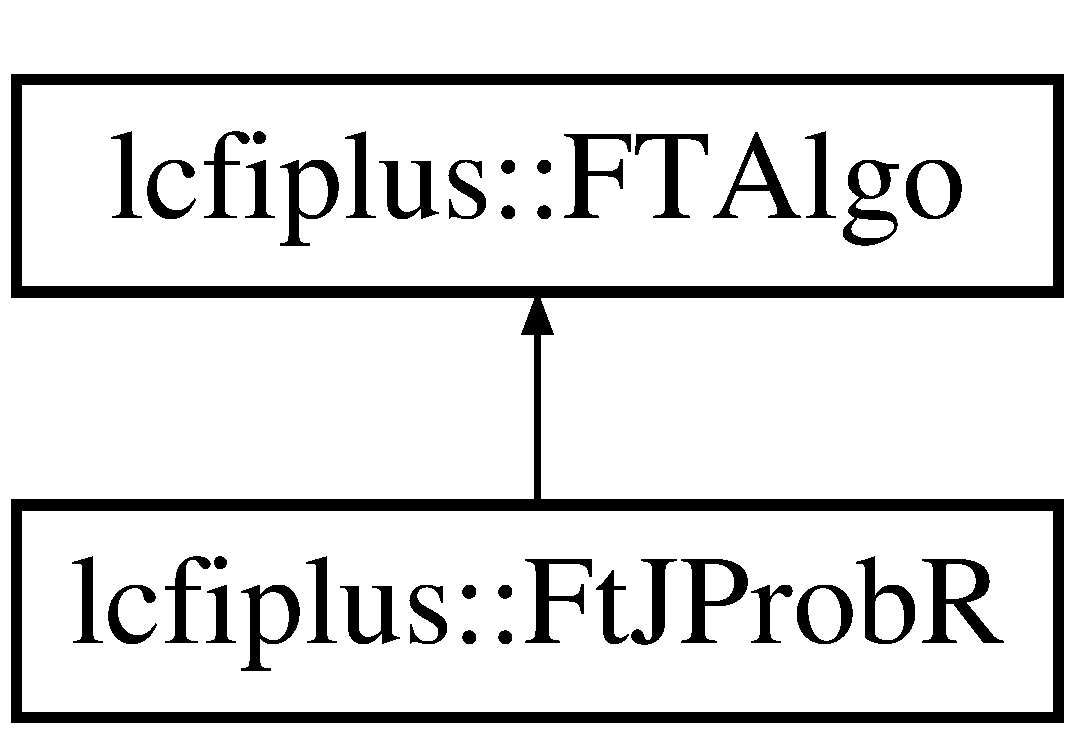
\includegraphics[height=2.000000cm]{classlcfiplus_1_1FtJProbR}
\end{center}
\end{figure}
\subsection*{Public Member Functions}
\begin{DoxyCompactItemize}
\item 
{\bf Ft\-J\-Prob\-R} ()
\item 
void {\bf process} ()
\end{DoxyCompactItemize}
\subsection*{Additional Inherited Members}


\subsection{Constructor \& Destructor Documentation}
\index{lcfiplus\-::\-Ft\-J\-Prob\-R@{lcfiplus\-::\-Ft\-J\-Prob\-R}!Ft\-J\-Prob\-R@{Ft\-J\-Prob\-R}}
\index{Ft\-J\-Prob\-R@{Ft\-J\-Prob\-R}!lcfiplus::FtJProbR@{lcfiplus\-::\-Ft\-J\-Prob\-R}}
\subsubsection[{Ft\-J\-Prob\-R}]{\setlength{\rightskip}{0pt plus 5cm}lcfiplus\-::\-Ft\-J\-Prob\-R\-::\-Ft\-J\-Prob\-R (
\begin{DoxyParamCaption}
{}
\end{DoxyParamCaption}
)\hspace{0.3cm}{\ttfamily [inline]}}\label{classlcfiplus_1_1FtJProbR_a49edffa52bb373728dc98ab7d304ffd4}


\subsection{Member Function Documentation}
\index{lcfiplus\-::\-Ft\-J\-Prob\-R@{lcfiplus\-::\-Ft\-J\-Prob\-R}!process@{process}}
\index{process@{process}!lcfiplus::FtJProbR@{lcfiplus\-::\-Ft\-J\-Prob\-R}}
\subsubsection[{process}]{\setlength{\rightskip}{0pt plus 5cm}void lcfiplus\-::\-Ft\-J\-Prob\-R\-::process (
\begin{DoxyParamCaption}
{}
\end{DoxyParamCaption}
)\hspace{0.3cm}{\ttfamily [inline]}, {\ttfamily [virtual]}}\label{classlcfiplus_1_1FtJProbR_a8bca5390b49033530ceec071aca60762}


Reimplemented from {\bf lcfiplus\-::\-F\-T\-Algo} \doxyref{}{p.}{classlcfiplus_1_1FTAlgo_a23cc3f3cd1c100ab6b5e16056112351a}.



References lcfiplus\-::algo\-Sig\-Prob\-::joint\-Prob\-D0().



The documentation for this class was generated from the following file\-:\begin{DoxyCompactItemize}
\item 
{\bf Flavor\-Tag.\-cc}\end{DoxyCompactItemize}

\section{lcfiplus\-:\-:Ft\-J\-Prob\-R2 Class Reference}
\label{classlcfiplus_1_1FtJProbR2}\index{lcfiplus\-::\-Ft\-J\-Prob\-R2@{lcfiplus\-::\-Ft\-J\-Prob\-R2}}
Inheritance diagram for lcfiplus\-:\-:Ft\-J\-Prob\-R2\-:\begin{figure}[H]
\begin{center}
\leavevmode
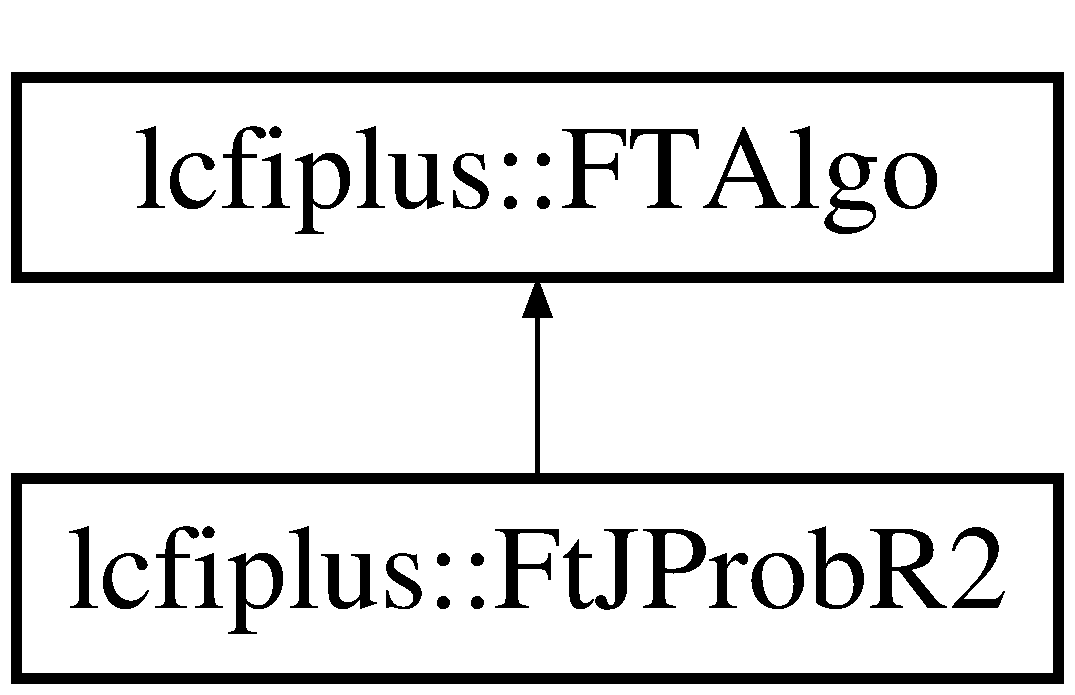
\includegraphics[height=2.000000cm]{classlcfiplus_1_1FtJProbR2}
\end{center}
\end{figure}
\subsection*{Public Member Functions}
\begin{DoxyCompactItemize}
\item 
{\bf Ft\-J\-Prob\-R2} ()
\item 
void {\bf process} ()
\end{DoxyCompactItemize}
\subsection*{Additional Inherited Members}


\subsection{Constructor \& Destructor Documentation}
\index{lcfiplus\-::\-Ft\-J\-Prob\-R2@{lcfiplus\-::\-Ft\-J\-Prob\-R2}!Ft\-J\-Prob\-R2@{Ft\-J\-Prob\-R2}}
\index{Ft\-J\-Prob\-R2@{Ft\-J\-Prob\-R2}!lcfiplus::FtJProbR2@{lcfiplus\-::\-Ft\-J\-Prob\-R2}}
\subsubsection[{Ft\-J\-Prob\-R2}]{\setlength{\rightskip}{0pt plus 5cm}lcfiplus\-::\-Ft\-J\-Prob\-R2\-::\-Ft\-J\-Prob\-R2 (
\begin{DoxyParamCaption}
{}
\end{DoxyParamCaption}
)\hspace{0.3cm}{\ttfamily [inline]}}\label{classlcfiplus_1_1FtJProbR2_a72dfe2871dea5402f8be51232a05d77a}


\subsection{Member Function Documentation}
\index{lcfiplus\-::\-Ft\-J\-Prob\-R2@{lcfiplus\-::\-Ft\-J\-Prob\-R2}!process@{process}}
\index{process@{process}!lcfiplus::FtJProbR2@{lcfiplus\-::\-Ft\-J\-Prob\-R2}}
\subsubsection[{process}]{\setlength{\rightskip}{0pt plus 5cm}void lcfiplus\-::\-Ft\-J\-Prob\-R2\-::process (
\begin{DoxyParamCaption}
{}
\end{DoxyParamCaption}
)\hspace{0.3cm}{\ttfamily [inline]}, {\ttfamily [virtual]}}\label{classlcfiplus_1_1FtJProbR2_abdc160e02a597230ffead6a04147e9f4}


Reimplemented from {\bf lcfiplus\-::\-F\-T\-Algo} \doxyref{}{p.}{classlcfiplus_1_1FTAlgo_a23cc3f3cd1c100ab6b5e16056112351a}.



References lcfiplus\-::\-F\-T\-Manager\-::get\-Instance(), lcfiplus\-::\-F\-T\-Manager\-::get\-I\-P\-Prob\-Holder(), and lcfiplus\-::algo\-Sig\-Prob\-::joint\-Prob2\-D0().



The documentation for this class was generated from the following file\-:\begin{DoxyCompactItemize}
\item 
{\bf Flavor\-Tag.\-cc}\end{DoxyCompactItemize}

\section{lcfiplus\-:\-:Ft\-J\-Prob\-R25\-Sigma Class Reference}
\label{classlcfiplus_1_1FtJProbR25Sigma}\index{lcfiplus\-::\-Ft\-J\-Prob\-R25\-Sigma@{lcfiplus\-::\-Ft\-J\-Prob\-R25\-Sigma}}
Inheritance diagram for lcfiplus\-:\-:Ft\-J\-Prob\-R25\-Sigma\-:\begin{figure}[H]
\begin{center}
\leavevmode
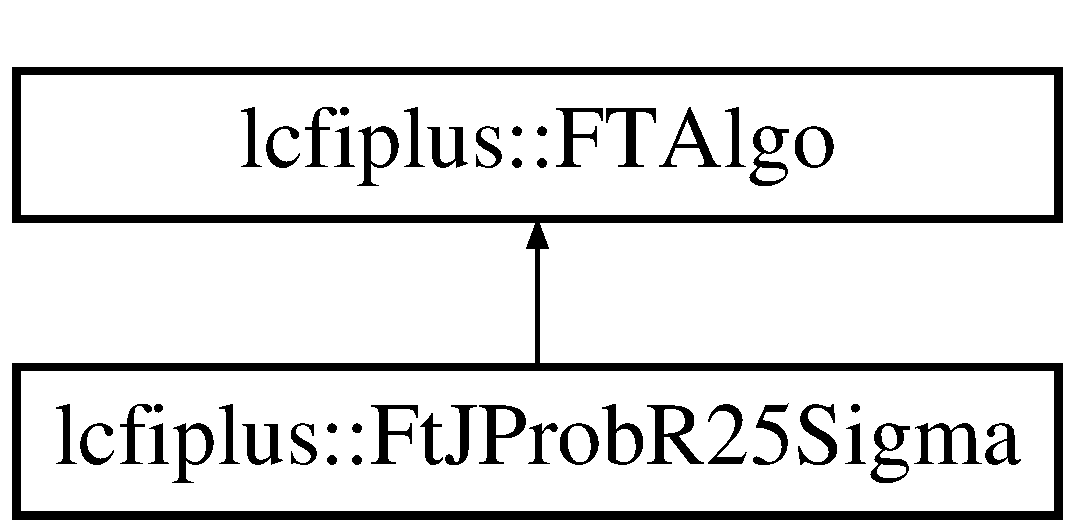
\includegraphics[height=2.000000cm]{classlcfiplus_1_1FtJProbR25Sigma}
\end{center}
\end{figure}
\subsection*{Public Member Functions}
\begin{DoxyCompactItemize}
\item 
{\bf Ft\-J\-Prob\-R25\-Sigma} (bool usevt)
\item 
void {\bf process} ()
\end{DoxyCompactItemize}
\subsection*{Additional Inherited Members}


\subsection{Constructor \& Destructor Documentation}
\index{lcfiplus\-::\-Ft\-J\-Prob\-R25\-Sigma@{lcfiplus\-::\-Ft\-J\-Prob\-R25\-Sigma}!Ft\-J\-Prob\-R25\-Sigma@{Ft\-J\-Prob\-R25\-Sigma}}
\index{Ft\-J\-Prob\-R25\-Sigma@{Ft\-J\-Prob\-R25\-Sigma}!lcfiplus::FtJProbR25Sigma@{lcfiplus\-::\-Ft\-J\-Prob\-R25\-Sigma}}
\subsubsection[{Ft\-J\-Prob\-R25\-Sigma}]{\setlength{\rightskip}{0pt plus 5cm}lcfiplus\-::\-Ft\-J\-Prob\-R25\-Sigma\-::\-Ft\-J\-Prob\-R25\-Sigma (
\begin{DoxyParamCaption}
\item[{bool}]{usevt}
\end{DoxyParamCaption}
)\hspace{0.3cm}{\ttfamily [inline]}}\label{classlcfiplus_1_1FtJProbR25Sigma_ab4c2dd8c2cd26d50deb08e9d510c9c4a}


\subsection{Member Function Documentation}
\index{lcfiplus\-::\-Ft\-J\-Prob\-R25\-Sigma@{lcfiplus\-::\-Ft\-J\-Prob\-R25\-Sigma}!process@{process}}
\index{process@{process}!lcfiplus::FtJProbR25Sigma@{lcfiplus\-::\-Ft\-J\-Prob\-R25\-Sigma}}
\subsubsection[{process}]{\setlength{\rightskip}{0pt plus 5cm}void lcfiplus\-::\-Ft\-J\-Prob\-R25\-Sigma\-::process (
\begin{DoxyParamCaption}
{}
\end{DoxyParamCaption}
)\hspace{0.3cm}{\ttfamily [inline]}, {\ttfamily [virtual]}}\label{classlcfiplus_1_1FtJProbR25Sigma_a4023aebf51a661e640842bf6006facaa}


Reimplemented from {\bf lcfiplus\-::\-F\-T\-Algo} \doxyref{}{p.}{classlcfiplus_1_1FTAlgo_a23cc3f3cd1c100ab6b5e16056112351a}.



References lcfiplus\-::\-F\-T\-Manager\-::get\-Instance(), lcfiplus\-::\-F\-T\-Manager\-::get\-I\-P\-Prob\-Holder(), and lcfiplus\-::algo\-Sig\-Prob\-::joint\-Prob2\-D0().



The documentation for this class was generated from the following file\-:\begin{DoxyCompactItemize}
\item 
{\bf Flavor\-Tag.\-cc}\end{DoxyCompactItemize}

\section{lcfiplus\-:\-:Ft\-J\-Prob\-R5\-Sigma Class Reference}
\label{classlcfiplus_1_1FtJProbR5Sigma}\index{lcfiplus\-::\-Ft\-J\-Prob\-R5\-Sigma@{lcfiplus\-::\-Ft\-J\-Prob\-R5\-Sigma}}
Inheritance diagram for lcfiplus\-:\-:Ft\-J\-Prob\-R5\-Sigma\-:\begin{figure}[H]
\begin{center}
\leavevmode
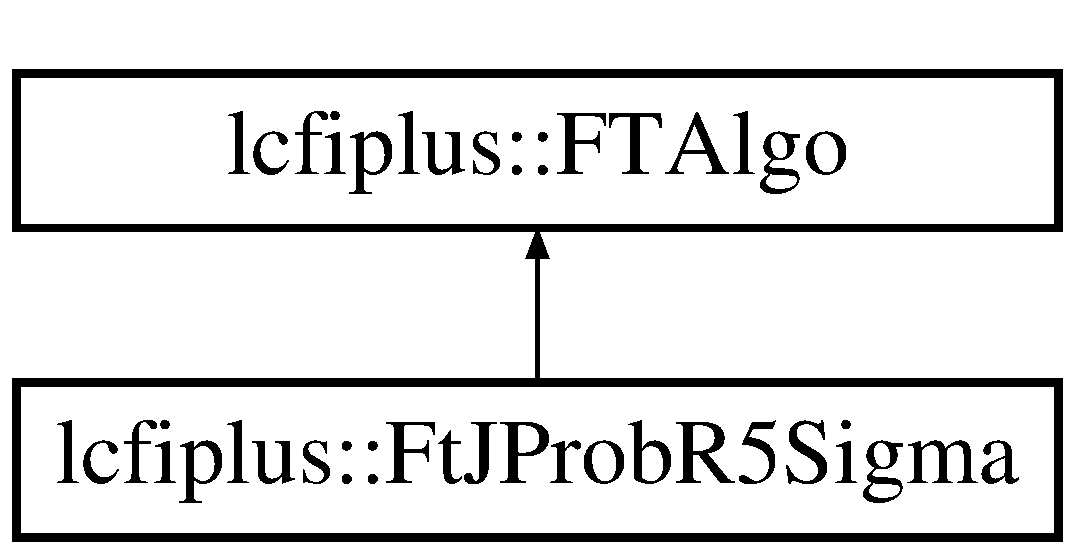
\includegraphics[height=2.000000cm]{classlcfiplus_1_1FtJProbR5Sigma}
\end{center}
\end{figure}
\subsection*{Public Member Functions}
\begin{DoxyCompactItemize}
\item 
{\bf Ft\-J\-Prob\-R5\-Sigma} (bool usevt)
\item 
void {\bf process} ()
\end{DoxyCompactItemize}
\subsection*{Additional Inherited Members}


\subsection{Constructor \& Destructor Documentation}
\index{lcfiplus\-::\-Ft\-J\-Prob\-R5\-Sigma@{lcfiplus\-::\-Ft\-J\-Prob\-R5\-Sigma}!Ft\-J\-Prob\-R5\-Sigma@{Ft\-J\-Prob\-R5\-Sigma}}
\index{Ft\-J\-Prob\-R5\-Sigma@{Ft\-J\-Prob\-R5\-Sigma}!lcfiplus::FtJProbR5Sigma@{lcfiplus\-::\-Ft\-J\-Prob\-R5\-Sigma}}
\subsubsection[{Ft\-J\-Prob\-R5\-Sigma}]{\setlength{\rightskip}{0pt plus 5cm}lcfiplus\-::\-Ft\-J\-Prob\-R5\-Sigma\-::\-Ft\-J\-Prob\-R5\-Sigma (
\begin{DoxyParamCaption}
\item[{bool}]{usevt}
\end{DoxyParamCaption}
)\hspace{0.3cm}{\ttfamily [inline]}}\label{classlcfiplus_1_1FtJProbR5Sigma_a0be88d936f11f80b47c78aef94ed7b12}


\subsection{Member Function Documentation}
\index{lcfiplus\-::\-Ft\-J\-Prob\-R5\-Sigma@{lcfiplus\-::\-Ft\-J\-Prob\-R5\-Sigma}!process@{process}}
\index{process@{process}!lcfiplus::FtJProbR5Sigma@{lcfiplus\-::\-Ft\-J\-Prob\-R5\-Sigma}}
\subsubsection[{process}]{\setlength{\rightskip}{0pt plus 5cm}void lcfiplus\-::\-Ft\-J\-Prob\-R5\-Sigma\-::process (
\begin{DoxyParamCaption}
{}
\end{DoxyParamCaption}
)\hspace{0.3cm}{\ttfamily [inline]}, {\ttfamily [virtual]}}\label{classlcfiplus_1_1FtJProbR5Sigma_aeaf2eec741c8f11a7534eac003401007}


Reimplemented from {\bf lcfiplus\-::\-F\-T\-Algo} \doxyref{}{p.}{classlcfiplus_1_1FTAlgo_a23cc3f3cd1c100ab6b5e16056112351a}.



References lcfiplus\-::algo\-Sig\-Prob\-::joint\-Prob\-D0().



The documentation for this class was generated from the following file\-:\begin{DoxyCompactItemize}
\item 
{\bf Flavor\-Tag.\-cc}\end{DoxyCompactItemize}

\section{lcfiplus\-:\-:Ft\-J\-Prob\-Z Class Reference}
\label{classlcfiplus_1_1FtJProbZ}\index{lcfiplus\-::\-Ft\-J\-Prob\-Z@{lcfiplus\-::\-Ft\-J\-Prob\-Z}}
Inheritance diagram for lcfiplus\-:\-:Ft\-J\-Prob\-Z\-:\begin{figure}[H]
\begin{center}
\leavevmode
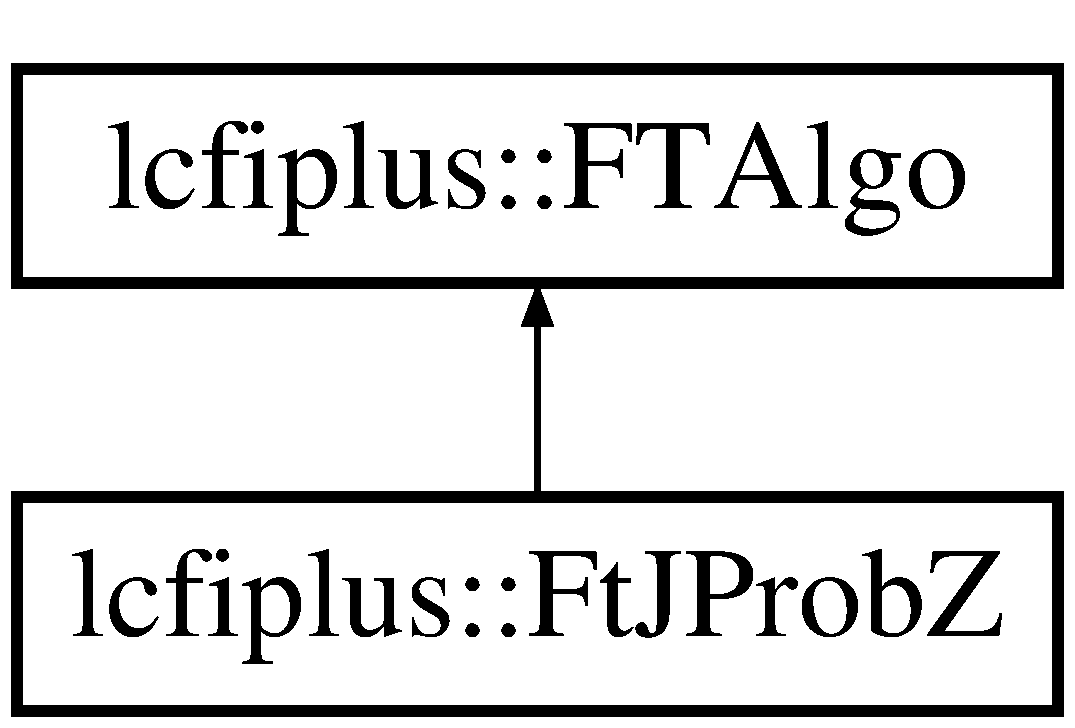
\includegraphics[height=2.000000cm]{classlcfiplus_1_1FtJProbZ}
\end{center}
\end{figure}
\subsection*{Public Member Functions}
\begin{DoxyCompactItemize}
\item 
{\bf Ft\-J\-Prob\-Z} ()
\item 
void {\bf process} ()
\end{DoxyCompactItemize}
\subsection*{Additional Inherited Members}


\subsection{Constructor \& Destructor Documentation}
\index{lcfiplus\-::\-Ft\-J\-Prob\-Z@{lcfiplus\-::\-Ft\-J\-Prob\-Z}!Ft\-J\-Prob\-Z@{Ft\-J\-Prob\-Z}}
\index{Ft\-J\-Prob\-Z@{Ft\-J\-Prob\-Z}!lcfiplus::FtJProbZ@{lcfiplus\-::\-Ft\-J\-Prob\-Z}}
\subsubsection[{Ft\-J\-Prob\-Z}]{\setlength{\rightskip}{0pt plus 5cm}lcfiplus\-::\-Ft\-J\-Prob\-Z\-::\-Ft\-J\-Prob\-Z (
\begin{DoxyParamCaption}
{}
\end{DoxyParamCaption}
)\hspace{0.3cm}{\ttfamily [inline]}}\label{classlcfiplus_1_1FtJProbZ_abbe6439c38f12fad63dfa784fd2515b2}


\subsection{Member Function Documentation}
\index{lcfiplus\-::\-Ft\-J\-Prob\-Z@{lcfiplus\-::\-Ft\-J\-Prob\-Z}!process@{process}}
\index{process@{process}!lcfiplus::FtJProbZ@{lcfiplus\-::\-Ft\-J\-Prob\-Z}}
\subsubsection[{process}]{\setlength{\rightskip}{0pt plus 5cm}void lcfiplus\-::\-Ft\-J\-Prob\-Z\-::process (
\begin{DoxyParamCaption}
{}
\end{DoxyParamCaption}
)\hspace{0.3cm}{\ttfamily [inline]}, {\ttfamily [virtual]}}\label{classlcfiplus_1_1FtJProbZ_aeae617aa635e1ec77a4ab1235448ac35}


Reimplemented from {\bf lcfiplus\-::\-F\-T\-Algo} \doxyref{}{p.}{classlcfiplus_1_1FTAlgo_a23cc3f3cd1c100ab6b5e16056112351a}.



References lcfiplus\-::algo\-Sig\-Prob\-::joint\-Prob\-Z0().



The documentation for this class was generated from the following file\-:\begin{DoxyCompactItemize}
\item 
{\bf Flavor\-Tag.\-cc}\end{DoxyCompactItemize}

\section{lcfiplus\-:\-:Ft\-J\-Prob\-Z2 Class Reference}
\label{classlcfiplus_1_1FtJProbZ2}\index{lcfiplus\-::\-Ft\-J\-Prob\-Z2@{lcfiplus\-::\-Ft\-J\-Prob\-Z2}}
Inheritance diagram for lcfiplus\-:\-:Ft\-J\-Prob\-Z2\-:\begin{figure}[H]
\begin{center}
\leavevmode
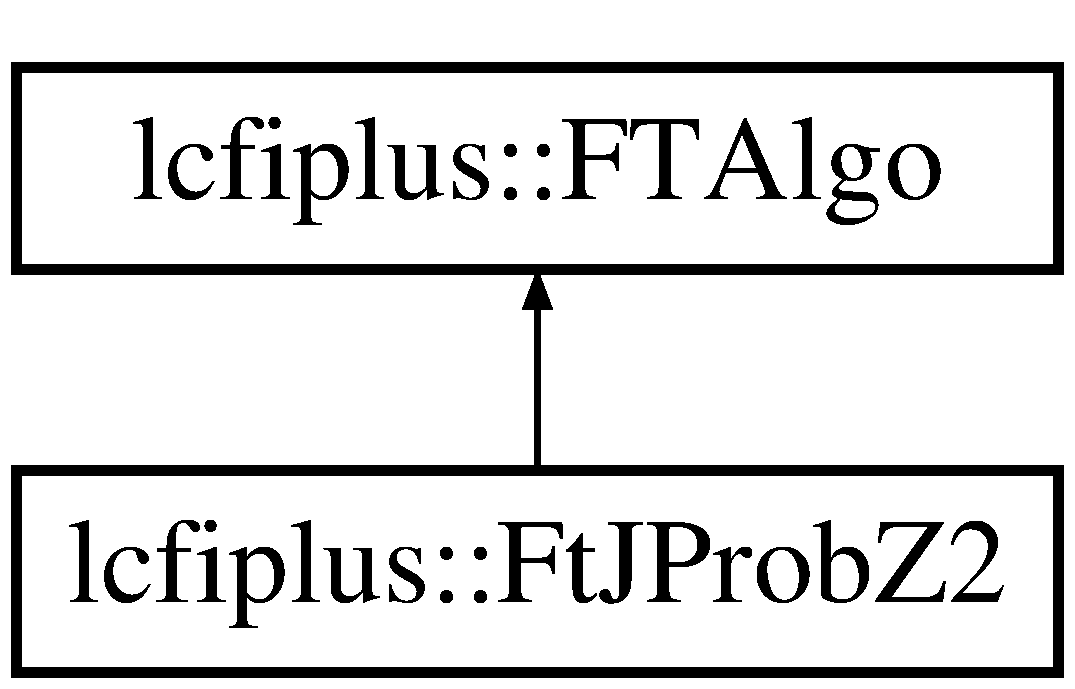
\includegraphics[height=2.000000cm]{classlcfiplus_1_1FtJProbZ2}
\end{center}
\end{figure}
\subsection*{Public Member Functions}
\begin{DoxyCompactItemize}
\item 
{\bf Ft\-J\-Prob\-Z2} ()
\item 
void {\bf process} ()
\end{DoxyCompactItemize}
\subsection*{Additional Inherited Members}


\subsection{Constructor \& Destructor Documentation}
\index{lcfiplus\-::\-Ft\-J\-Prob\-Z2@{lcfiplus\-::\-Ft\-J\-Prob\-Z2}!Ft\-J\-Prob\-Z2@{Ft\-J\-Prob\-Z2}}
\index{Ft\-J\-Prob\-Z2@{Ft\-J\-Prob\-Z2}!lcfiplus::FtJProbZ2@{lcfiplus\-::\-Ft\-J\-Prob\-Z2}}
\subsubsection[{Ft\-J\-Prob\-Z2}]{\setlength{\rightskip}{0pt plus 5cm}lcfiplus\-::\-Ft\-J\-Prob\-Z2\-::\-Ft\-J\-Prob\-Z2 (
\begin{DoxyParamCaption}
{}
\end{DoxyParamCaption}
)\hspace{0.3cm}{\ttfamily [inline]}}\label{classlcfiplus_1_1FtJProbZ2_a54fcdd7b189c7f7ea16c533cc96fd42b}


\subsection{Member Function Documentation}
\index{lcfiplus\-::\-Ft\-J\-Prob\-Z2@{lcfiplus\-::\-Ft\-J\-Prob\-Z2}!process@{process}}
\index{process@{process}!lcfiplus::FtJProbZ2@{lcfiplus\-::\-Ft\-J\-Prob\-Z2}}
\subsubsection[{process}]{\setlength{\rightskip}{0pt plus 5cm}void lcfiplus\-::\-Ft\-J\-Prob\-Z2\-::process (
\begin{DoxyParamCaption}
{}
\end{DoxyParamCaption}
)\hspace{0.3cm}{\ttfamily [inline]}, {\ttfamily [virtual]}}\label{classlcfiplus_1_1FtJProbZ2_a8fcb9cd0ca85e631f6ebba7dd8681f0c}


Reimplemented from {\bf lcfiplus\-::\-F\-T\-Algo} \doxyref{}{p.}{classlcfiplus_1_1FTAlgo_a23cc3f3cd1c100ab6b5e16056112351a}.



References lcfiplus\-::\-F\-T\-Manager\-::get\-Instance(), lcfiplus\-::\-F\-T\-Manager\-::get\-I\-P\-Prob\-Holder(), and lcfiplus\-::algo\-Sig\-Prob\-::joint\-Prob2\-Z0().



The documentation for this class was generated from the following file\-:\begin{DoxyCompactItemize}
\item 
{\bf Flavor\-Tag.\-cc}\end{DoxyCompactItemize}

\section{lcfiplus\-:\-:Ft\-J\-Prob\-Z25\-Sigma Class Reference}
\label{classlcfiplus_1_1FtJProbZ25Sigma}\index{lcfiplus\-::\-Ft\-J\-Prob\-Z25\-Sigma@{lcfiplus\-::\-Ft\-J\-Prob\-Z25\-Sigma}}
Inheritance diagram for lcfiplus\-:\-:Ft\-J\-Prob\-Z25\-Sigma\-:\begin{figure}[H]
\begin{center}
\leavevmode
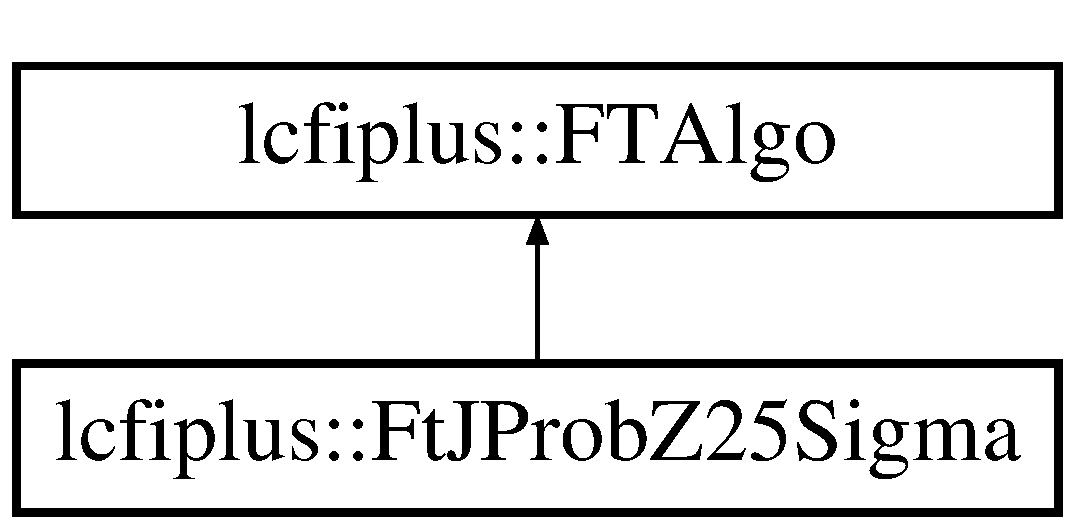
\includegraphics[height=2.000000cm]{classlcfiplus_1_1FtJProbZ25Sigma}
\end{center}
\end{figure}
\subsection*{Public Member Functions}
\begin{DoxyCompactItemize}
\item 
{\bf Ft\-J\-Prob\-Z25\-Sigma} (bool usevt)
\item 
void {\bf process} ()
\end{DoxyCompactItemize}
\subsection*{Public Attributes}
\begin{DoxyCompactItemize}
\item 
bool {\bf \-\_\-use\-Vertex\-Tracks}
\end{DoxyCompactItemize}
\subsection*{Additional Inherited Members}


\subsection{Constructor \& Destructor Documentation}
\index{lcfiplus\-::\-Ft\-J\-Prob\-Z25\-Sigma@{lcfiplus\-::\-Ft\-J\-Prob\-Z25\-Sigma}!Ft\-J\-Prob\-Z25\-Sigma@{Ft\-J\-Prob\-Z25\-Sigma}}
\index{Ft\-J\-Prob\-Z25\-Sigma@{Ft\-J\-Prob\-Z25\-Sigma}!lcfiplus::FtJProbZ25Sigma@{lcfiplus\-::\-Ft\-J\-Prob\-Z25\-Sigma}}
\subsubsection[{Ft\-J\-Prob\-Z25\-Sigma}]{\setlength{\rightskip}{0pt plus 5cm}lcfiplus\-::\-Ft\-J\-Prob\-Z25\-Sigma\-::\-Ft\-J\-Prob\-Z25\-Sigma (
\begin{DoxyParamCaption}
\item[{bool}]{usevt}
\end{DoxyParamCaption}
)\hspace{0.3cm}{\ttfamily [inline]}}\label{classlcfiplus_1_1FtJProbZ25Sigma_ad060807b2d688149b9edd2628cf898d3}


\subsection{Member Function Documentation}
\index{lcfiplus\-::\-Ft\-J\-Prob\-Z25\-Sigma@{lcfiplus\-::\-Ft\-J\-Prob\-Z25\-Sigma}!process@{process}}
\index{process@{process}!lcfiplus::FtJProbZ25Sigma@{lcfiplus\-::\-Ft\-J\-Prob\-Z25\-Sigma}}
\subsubsection[{process}]{\setlength{\rightskip}{0pt plus 5cm}void lcfiplus\-::\-Ft\-J\-Prob\-Z25\-Sigma\-::process (
\begin{DoxyParamCaption}
{}
\end{DoxyParamCaption}
)\hspace{0.3cm}{\ttfamily [inline]}, {\ttfamily [virtual]}}\label{classlcfiplus_1_1FtJProbZ25Sigma_a166ae515e6a478e74877d5ed2db243bf}


Reimplemented from {\bf lcfiplus\-::\-F\-T\-Algo} \doxyref{}{p.}{classlcfiplus_1_1FTAlgo_a23cc3f3cd1c100ab6b5e16056112351a}.



References lcfiplus\-::\-F\-T\-Manager\-::get\-Instance(), lcfiplus\-::\-F\-T\-Manager\-::get\-I\-P\-Prob\-Holder(), and lcfiplus\-::algo\-Sig\-Prob\-::joint\-Prob2\-Z0().



\subsection{Member Data Documentation}
\index{lcfiplus\-::\-Ft\-J\-Prob\-Z25\-Sigma@{lcfiplus\-::\-Ft\-J\-Prob\-Z25\-Sigma}!\-\_\-use\-Vertex\-Tracks@{\-\_\-use\-Vertex\-Tracks}}
\index{\-\_\-use\-Vertex\-Tracks@{\-\_\-use\-Vertex\-Tracks}!lcfiplus::FtJProbZ25Sigma@{lcfiplus\-::\-Ft\-J\-Prob\-Z25\-Sigma}}
\subsubsection[{\-\_\-use\-Vertex\-Tracks}]{\setlength{\rightskip}{0pt plus 5cm}bool lcfiplus\-::\-Ft\-J\-Prob\-Z25\-Sigma\-::\-\_\-use\-Vertex\-Tracks}\label{classlcfiplus_1_1FtJProbZ25Sigma_a52e1e3b0e5335d63820fe99232221b3d}


The documentation for this class was generated from the following file\-:\begin{DoxyCompactItemize}
\item 
{\bf Flavor\-Tag.\-cc}\end{DoxyCompactItemize}

\section{lcfiplus\-:\-:Ft\-J\-Prob\-Z5\-Sigma Class Reference}
\label{classlcfiplus_1_1FtJProbZ5Sigma}\index{lcfiplus\-::\-Ft\-J\-Prob\-Z5\-Sigma@{lcfiplus\-::\-Ft\-J\-Prob\-Z5\-Sigma}}
Inheritance diagram for lcfiplus\-:\-:Ft\-J\-Prob\-Z5\-Sigma\-:\begin{figure}[H]
\begin{center}
\leavevmode
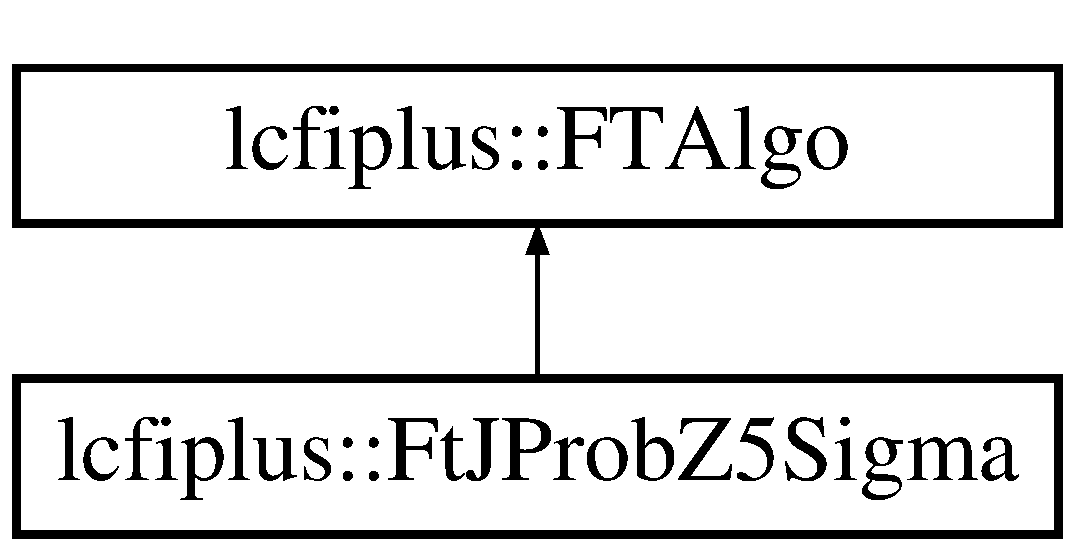
\includegraphics[height=2.000000cm]{classlcfiplus_1_1FtJProbZ5Sigma}
\end{center}
\end{figure}
\subsection*{Public Member Functions}
\begin{DoxyCompactItemize}
\item 
{\bf Ft\-J\-Prob\-Z5\-Sigma} (bool usevt)
\item 
void {\bf process} ()
\end{DoxyCompactItemize}
\subsection*{Public Attributes}
\begin{DoxyCompactItemize}
\item 
bool {\bf \-\_\-use\-Vertex\-Tracks}
\end{DoxyCompactItemize}
\subsection*{Additional Inherited Members}


\subsection{Constructor \& Destructor Documentation}
\index{lcfiplus\-::\-Ft\-J\-Prob\-Z5\-Sigma@{lcfiplus\-::\-Ft\-J\-Prob\-Z5\-Sigma}!Ft\-J\-Prob\-Z5\-Sigma@{Ft\-J\-Prob\-Z5\-Sigma}}
\index{Ft\-J\-Prob\-Z5\-Sigma@{Ft\-J\-Prob\-Z5\-Sigma}!lcfiplus::FtJProbZ5Sigma@{lcfiplus\-::\-Ft\-J\-Prob\-Z5\-Sigma}}
\subsubsection[{Ft\-J\-Prob\-Z5\-Sigma}]{\setlength{\rightskip}{0pt plus 5cm}lcfiplus\-::\-Ft\-J\-Prob\-Z5\-Sigma\-::\-Ft\-J\-Prob\-Z5\-Sigma (
\begin{DoxyParamCaption}
\item[{bool}]{usevt}
\end{DoxyParamCaption}
)\hspace{0.3cm}{\ttfamily [inline]}}\label{classlcfiplus_1_1FtJProbZ5Sigma_a180c4a277bbf32c9e336a34ab3c6c8d1}


\subsection{Member Function Documentation}
\index{lcfiplus\-::\-Ft\-J\-Prob\-Z5\-Sigma@{lcfiplus\-::\-Ft\-J\-Prob\-Z5\-Sigma}!process@{process}}
\index{process@{process}!lcfiplus::FtJProbZ5Sigma@{lcfiplus\-::\-Ft\-J\-Prob\-Z5\-Sigma}}
\subsubsection[{process}]{\setlength{\rightskip}{0pt plus 5cm}void lcfiplus\-::\-Ft\-J\-Prob\-Z5\-Sigma\-::process (
\begin{DoxyParamCaption}
{}
\end{DoxyParamCaption}
)\hspace{0.3cm}{\ttfamily [inline]}, {\ttfamily [virtual]}}\label{classlcfiplus_1_1FtJProbZ5Sigma_acabdb6a10a791978f4fdf5c77111726d}


Reimplemented from {\bf lcfiplus\-::\-F\-T\-Algo} \doxyref{}{p.}{classlcfiplus_1_1FTAlgo_a23cc3f3cd1c100ab6b5e16056112351a}.



References lcfiplus\-::algo\-Sig\-Prob\-::joint\-Prob\-Z0().



\subsection{Member Data Documentation}
\index{lcfiplus\-::\-Ft\-J\-Prob\-Z5\-Sigma@{lcfiplus\-::\-Ft\-J\-Prob\-Z5\-Sigma}!\-\_\-use\-Vertex\-Tracks@{\-\_\-use\-Vertex\-Tracks}}
\index{\-\_\-use\-Vertex\-Tracks@{\-\_\-use\-Vertex\-Tracks}!lcfiplus::FtJProbZ5Sigma@{lcfiplus\-::\-Ft\-J\-Prob\-Z5\-Sigma}}
\subsubsection[{\-\_\-use\-Vertex\-Tracks}]{\setlength{\rightskip}{0pt plus 5cm}bool lcfiplus\-::\-Ft\-J\-Prob\-Z5\-Sigma\-::\-\_\-use\-Vertex\-Tracks}\label{classlcfiplus_1_1FtJProbZ5Sigma_adc60ab341edd6d124bb8a32b3f000525}


The documentation for this class was generated from the following file\-:\begin{DoxyCompactItemize}
\item 
{\bf Flavor\-Tag.\-cc}\end{DoxyCompactItemize}

\section{lcfiplus\-:\-:F\-T\-Manager Class Reference}
\label{classlcfiplus_1_1FTManager}\index{lcfiplus\-::\-F\-T\-Manager@{lcfiplus\-::\-F\-T\-Manager}}


{\ttfamily \#include $<$flavtag.\-h$>$}

\subsection*{Public Member Functions}
\begin{DoxyCompactItemize}
\item 
void {\bf init\-Vars} ()
\item 
void {\bf fill\-Tree} ()
\item 
void {\bf open\-Tree} ()
\item 
void {\bf open\-File} (const char $\ast$filename)
\item 
void {\bf close\-File} ()
\item 
void {\bf process} (const {\bf Event} $\ast$event, const {\bf Vertex} $\ast$privtx, int nhits\-Joint\-Prob\-D0, int nhits\-Joint\-Prob\-Z0, int nhits\-Most\-Significant\-Track, {\bf Jet\-Vec} \&jets)
\item 
float $\ast$ {\bf get\-Var\-Address} (const string \&varname)
\item 
void {\bf set\-Eval} (bool seteval, bool export\-All\-Vars)
\item 
void {\bf add\-Reader} (T\-M\-V\-A\-::\-Reader $\ast$reader, const {\bf Flavtag\-Category} \&c)
\item 
void {\bf set\-Param\-Name} (T\-String s)
\item 
const {\bf Ft\-I\-P\-Prob\-Holder} $\ast$ {\bf get\-I\-P\-Prob\-Holder} () const 
\item 
void {\bf set\-I\-P\-Prob\-Holder} ({\bf Ft\-I\-P\-Prob\-Holder} $\ast$holder)
\item 
double {\bf get\-Auxiliary} () const 
\item 
void {\bf set\-Auxiliary} (double aux)
\end{DoxyCompactItemize}
\subsection*{Static Public Member Functions}
\begin{DoxyCompactItemize}
\item 
static {\bf F\-T\-Manager} \& {\bf get\-Instance} ()
\end{DoxyCompactItemize}


\subsection{Member Function Documentation}
\index{lcfiplus\-::\-F\-T\-Manager@{lcfiplus\-::\-F\-T\-Manager}!add\-Reader@{add\-Reader}}
\index{add\-Reader@{add\-Reader}!lcfiplus::FTManager@{lcfiplus\-::\-F\-T\-Manager}}
\subsubsection[{add\-Reader}]{\setlength{\rightskip}{0pt plus 5cm}void lcfiplus\-::\-F\-T\-Manager\-::add\-Reader (
\begin{DoxyParamCaption}
\item[{T\-M\-V\-A\-::\-Reader $\ast$}]{reader, }
\item[{const {\bf Flavtag\-Category} \&}]{c}
\end{DoxyParamCaption}
)}\label{classlcfiplus_1_1FTManager_a5dd1e2351bc025b6e96f8233af8bed17}


Referenced by lcfiplus\-::\-Read\-M\-V\-A\-::init().

\index{lcfiplus\-::\-F\-T\-Manager@{lcfiplus\-::\-F\-T\-Manager}!close\-File@{close\-File}}
\index{close\-File@{close\-File}!lcfiplus::FTManager@{lcfiplus\-::\-F\-T\-Manager}}
\subsubsection[{close\-File}]{\setlength{\rightskip}{0pt plus 5cm}void lcfiplus\-::\-F\-T\-Manager\-::close\-File (
\begin{DoxyParamCaption}
{}
\end{DoxyParamCaption}
)}\label{classlcfiplus_1_1FTManager_ada9310ab84f69d0a55268d908b4281ce}


Referenced by lcfiplus\-::\-Make\-Ntuple\-::end().

\index{lcfiplus\-::\-F\-T\-Manager@{lcfiplus\-::\-F\-T\-Manager}!fill\-Tree@{fill\-Tree}}
\index{fill\-Tree@{fill\-Tree}!lcfiplus::FTManager@{lcfiplus\-::\-F\-T\-Manager}}
\subsubsection[{fill\-Tree}]{\setlength{\rightskip}{0pt plus 5cm}void lcfiplus\-::\-F\-T\-Manager\-::fill\-Tree (
\begin{DoxyParamCaption}
{}
\end{DoxyParamCaption}
)}\label{classlcfiplus_1_1FTManager_a49959b6f525f8803142e99144283bde4}


Referenced by process().

\index{lcfiplus\-::\-F\-T\-Manager@{lcfiplus\-::\-F\-T\-Manager}!get\-Auxiliary@{get\-Auxiliary}}
\index{get\-Auxiliary@{get\-Auxiliary}!lcfiplus::FTManager@{lcfiplus\-::\-F\-T\-Manager}}
\subsubsection[{get\-Auxiliary}]{\setlength{\rightskip}{0pt plus 5cm}double lcfiplus\-::\-F\-T\-Manager\-::get\-Auxiliary (
\begin{DoxyParamCaption}
{}
\end{DoxyParamCaption}
) const\hspace{0.3cm}{\ttfamily [inline]}}\label{classlcfiplus_1_1FTManager_a1f27b95bf569fa169d129fa3d38e52c1}


Referenced by lcfiplus\-::\-Ft\-Auxiliary\-M\-::process().

\index{lcfiplus\-::\-F\-T\-Manager@{lcfiplus\-::\-F\-T\-Manager}!get\-Instance@{get\-Instance}}
\index{get\-Instance@{get\-Instance}!lcfiplus::FTManager@{lcfiplus\-::\-F\-T\-Manager}}
\subsubsection[{get\-Instance}]{\setlength{\rightskip}{0pt plus 5cm}static {\bf F\-T\-Manager}\& lcfiplus\-::\-F\-T\-Manager\-::get\-Instance (
\begin{DoxyParamCaption}
{}
\end{DoxyParamCaption}
)\hspace{0.3cm}{\ttfamily [inline]}, {\ttfamily [static]}}\label{classlcfiplus_1_1FTManager_adb1794dc4342b9fca995e77a9dbb580f}


Referenced by lcfiplus\-::\-Make\-Ntuple\-::end(), lcfiplus\-::\-Make\-Ntuple\-::init(), lcfiplus\-::\-Read\-M\-V\-A\-::init(), lcfiplus\-::\-Flavor\-Tag\-::init(), lcfiplus\-::\-Flavor\-Tag\-::process(), lcfiplus\-::\-Ft\-Auxiliary\-M\-::process(), lcfiplus\-::\-Ft\-J\-Prob\-R2\-::process(), lcfiplus\-::\-Ft\-J\-Prob\-Z2\-::process(), lcfiplus\-::\-Ft\-J\-Prob\-R25\-Sigma\-::process(), lcfiplus\-::\-Ft\-J\-Prob\-Z25\-Sigma\-::process(), lcfiplus\-::\-Ft\-D0b\-Prob\-::process(), lcfiplus\-::\-Ft\-D0b\-Prob2\-::process(), lcfiplus\-::\-Ft\-D0c\-Prob\-::process(), lcfiplus\-::\-Ft\-D0c\-Prob2\-::process(), lcfiplus\-::\-Ft\-D0q\-Prob\-::process(), lcfiplus\-::\-Ft\-D0q\-Prob2\-::process(), lcfiplus\-::\-Ft\-D0b\-Prob\-Signed\-::process(), lcfiplus\-::\-Ft\-D0c\-Prob\-Signed\-::process(), lcfiplus\-::\-Ft\-D0q\-Prob\-Signed\-::process(), lcfiplus\-::\-Ft\-D0b\-Prob\-I\-P\-::process(), lcfiplus\-::\-Ft\-D0c\-Prob\-I\-P\-::process(), lcfiplus\-::\-Ft\-Z0b\-Prob\-::process(), lcfiplus\-::\-Ft\-Z0b\-Prob2\-::process(), lcfiplus\-::\-Ft\-Z0c\-Prob\-::process(), lcfiplus\-::\-Ft\-Z0c\-Prob2\-::process(), lcfiplus\-::\-Ft\-Z0q\-Prob\-::process(), lcfiplus\-::\-Ft\-Z0q\-Prob2\-::process(), lcfiplus\-::\-Ft\-Z0b\-Prob\-I\-P\-::process(), and lcfiplus\-::\-Ft\-Z0c\-Prob\-I\-P\-::process().

\index{lcfiplus\-::\-F\-T\-Manager@{lcfiplus\-::\-F\-T\-Manager}!get\-I\-P\-Prob\-Holder@{get\-I\-P\-Prob\-Holder}}
\index{get\-I\-P\-Prob\-Holder@{get\-I\-P\-Prob\-Holder}!lcfiplus::FTManager@{lcfiplus\-::\-F\-T\-Manager}}
\subsubsection[{get\-I\-P\-Prob\-Holder}]{\setlength{\rightskip}{0pt plus 5cm}const {\bf Ft\-I\-P\-Prob\-Holder}$\ast$ lcfiplus\-::\-F\-T\-Manager\-::get\-I\-P\-Prob\-Holder (
\begin{DoxyParamCaption}
{}
\end{DoxyParamCaption}
) const\hspace{0.3cm}{\ttfamily [inline]}}\label{classlcfiplus_1_1FTManager_ad72e3200cabd4168695bcef556c89b1c}


Referenced by lcfiplus\-::\-Ft\-J\-Prob\-R2\-::process(), lcfiplus\-::\-Ft\-J\-Prob\-Z2\-::process(), lcfiplus\-::\-Ft\-J\-Prob\-R25\-Sigma\-::process(), lcfiplus\-::\-Ft\-J\-Prob\-Z25\-Sigma\-::process(), lcfiplus\-::\-Ft\-D0b\-Prob\-::process(), lcfiplus\-::\-Ft\-D0b\-Prob2\-::process(), lcfiplus\-::\-Ft\-D0c\-Prob\-::process(), lcfiplus\-::\-Ft\-D0c\-Prob2\-::process(), lcfiplus\-::\-Ft\-D0q\-Prob\-::process(), lcfiplus\-::\-Ft\-D0q\-Prob2\-::process(), lcfiplus\-::\-Ft\-D0b\-Prob\-Signed\-::process(), lcfiplus\-::\-Ft\-D0c\-Prob\-Signed\-::process(), lcfiplus\-::\-Ft\-D0q\-Prob\-Signed\-::process(), lcfiplus\-::\-Ft\-D0b\-Prob\-I\-P\-::process(), lcfiplus\-::\-Ft\-D0c\-Prob\-I\-P\-::process(), lcfiplus\-::\-Ft\-Z0b\-Prob\-::process(), lcfiplus\-::\-Ft\-Z0b\-Prob2\-::process(), lcfiplus\-::\-Ft\-Z0c\-Prob\-::process(), lcfiplus\-::\-Ft\-Z0c\-Prob2\-::process(), lcfiplus\-::\-Ft\-Z0q\-Prob\-::process(), lcfiplus\-::\-Ft\-Z0q\-Prob2\-::process(), lcfiplus\-::\-Ft\-Z0b\-Prob\-I\-P\-::process(), and lcfiplus\-::\-Ft\-Z0c\-Prob\-I\-P\-::process().

\index{lcfiplus\-::\-F\-T\-Manager@{lcfiplus\-::\-F\-T\-Manager}!get\-Var\-Address@{get\-Var\-Address}}
\index{get\-Var\-Address@{get\-Var\-Address}!lcfiplus::FTManager@{lcfiplus\-::\-F\-T\-Manager}}
\subsubsection[{get\-Var\-Address}]{\setlength{\rightskip}{0pt plus 5cm}float $\ast$ lcfiplus\-::\-F\-T\-Manager\-::get\-Var\-Address (
\begin{DoxyParamCaption}
\item[{const string \&}]{varname}
\end{DoxyParamCaption}
)}\label{classlcfiplus_1_1FTManager_a62ddf44a37554417ce3b31a9f7771cd9}


References lcfiplus\-::\-F\-T\-Algo\-::get\-Name(), and lcfiplus\-::\-F\-T\-Algo\-::get\-Value\-Address().



Referenced by lcfiplus\-::\-Read\-M\-V\-A\-::init().

\index{lcfiplus\-::\-F\-T\-Manager@{lcfiplus\-::\-F\-T\-Manager}!init\-Vars@{init\-Vars}}
\index{init\-Vars@{init\-Vars}!lcfiplus::FTManager@{lcfiplus\-::\-F\-T\-Manager}}
\subsubsection[{init\-Vars}]{\setlength{\rightskip}{0pt plus 5cm}void lcfiplus\-::\-F\-T\-Manager\-::init\-Vars (
\begin{DoxyParamCaption}
{}
\end{DoxyParamCaption}
)}\label{classlcfiplus_1_1FTManager_a8e1c87a7ae3abd38f49d54275659b972}


Referenced by lcfiplus\-::\-Flavor\-Tag\-::init().

\index{lcfiplus\-::\-F\-T\-Manager@{lcfiplus\-::\-F\-T\-Manager}!open\-File@{open\-File}}
\index{open\-File@{open\-File}!lcfiplus::FTManager@{lcfiplus\-::\-F\-T\-Manager}}
\subsubsection[{open\-File}]{\setlength{\rightskip}{0pt plus 5cm}void lcfiplus\-::\-F\-T\-Manager\-::open\-File (
\begin{DoxyParamCaption}
\item[{const char $\ast$}]{filename}
\end{DoxyParamCaption}
)}\label{classlcfiplus_1_1FTManager_a0bc30c3329fca1fa239d620fd2c5ebc4}


References lcfiplus\-::\-F\-T\-Algo\-::get\-Name(), and lcfiplus\-::\-F\-T\-Algo\-::get\-Value\-Address().



Referenced by lcfiplus\-::\-Make\-Ntuple\-::init().

\index{lcfiplus\-::\-F\-T\-Manager@{lcfiplus\-::\-F\-T\-Manager}!open\-Tree@{open\-Tree}}
\index{open\-Tree@{open\-Tree}!lcfiplus::FTManager@{lcfiplus\-::\-F\-T\-Manager}}
\subsubsection[{open\-Tree}]{\setlength{\rightskip}{0pt plus 5cm}void lcfiplus\-::\-F\-T\-Manager\-::open\-Tree (
\begin{DoxyParamCaption}
{}
\end{DoxyParamCaption}
)}\label{classlcfiplus_1_1FTManager_a77588e2cb1437933bfa798f8bf6a2229}


References lcfiplus\-::\-F\-T\-Algo\-::get\-Name(), and lcfiplus\-::\-F\-T\-Algo\-::get\-Value\-Address().



Referenced by lcfiplus\-::\-Read\-M\-V\-A\-::init().

\index{lcfiplus\-::\-F\-T\-Manager@{lcfiplus\-::\-F\-T\-Manager}!process@{process}}
\index{process@{process}!lcfiplus::FTManager@{lcfiplus\-::\-F\-T\-Manager}}
\subsubsection[{process}]{\setlength{\rightskip}{0pt plus 5cm}void lcfiplus\-::\-F\-T\-Manager\-::process (
\begin{DoxyParamCaption}
\item[{const {\bf Event} $\ast$}]{event, }
\item[{const {\bf Vertex} $\ast$}]{privtx, }
\item[{int}]{nhits\-Joint\-Prob\-D0, }
\item[{int}]{nhits\-Joint\-Prob\-Z0, }
\item[{int}]{nhits\-Most\-Significant\-Track, }
\item[{{\bf Jet\-Vec} \&}]{jets}
\end{DoxyParamCaption}
)}\label{classlcfiplus_1_1FTManager_a6b5c1f001fd8a802c21131d760a06254}


References lcfiplus\-::\-Parameters\-::add(), lcfiplus\-::\-Jet\-::add\-Param(), fill\-Tree(), lcfiplus\-::\-F\-T\-Algo\-::get\-Name(), lcfiplus\-::\-F\-T\-Algo\-::process(), lcfiplus\-::\-F\-T\-Algo\-::process\-Event(), lcfiplus\-::\-F\-T\-Algo\-::set\-Event(), lcfiplus\-::\-F\-T\-Algo\-::set\-Jet(), lcfiplus\-::\-F\-T\-Algo\-::set\-N\-Hits\-Joint\-Prob\-D0(), lcfiplus\-::\-F\-T\-Algo\-::set\-N\-Hits\-Joint\-Prob\-Z0(), and lcfiplus\-::\-F\-T\-Algo\-::set\-N\-Hits\-Most\-Significant\-Track().



Referenced by lcfiplus\-::\-Flavor\-Tag\-::process().

\index{lcfiplus\-::\-F\-T\-Manager@{lcfiplus\-::\-F\-T\-Manager}!set\-Auxiliary@{set\-Auxiliary}}
\index{set\-Auxiliary@{set\-Auxiliary}!lcfiplus::FTManager@{lcfiplus\-::\-F\-T\-Manager}}
\subsubsection[{set\-Auxiliary}]{\setlength{\rightskip}{0pt plus 5cm}void lcfiplus\-::\-F\-T\-Manager\-::set\-Auxiliary (
\begin{DoxyParamCaption}
\item[{double}]{aux}
\end{DoxyParamCaption}
)\hspace{0.3cm}{\ttfamily [inline]}}\label{classlcfiplus_1_1FTManager_acfe28cf6673eea93ca877cd6e16e901a}


Referenced by lcfiplus\-::\-Flavor\-Tag\-::process().

\index{lcfiplus\-::\-F\-T\-Manager@{lcfiplus\-::\-F\-T\-Manager}!set\-Eval@{set\-Eval}}
\index{set\-Eval@{set\-Eval}!lcfiplus::FTManager@{lcfiplus\-::\-F\-T\-Manager}}
\subsubsection[{set\-Eval}]{\setlength{\rightskip}{0pt plus 5cm}void lcfiplus\-::\-F\-T\-Manager\-::set\-Eval (
\begin{DoxyParamCaption}
\item[{bool}]{seteval, }
\item[{bool}]{export\-All\-Vars}
\end{DoxyParamCaption}
)\hspace{0.3cm}{\ttfamily [inline]}}\label{classlcfiplus_1_1FTManager_a1ba2d2473212c51bb60446455ed174e4}


Referenced by lcfiplus\-::\-Read\-M\-V\-A\-::init().

\index{lcfiplus\-::\-F\-T\-Manager@{lcfiplus\-::\-F\-T\-Manager}!set\-I\-P\-Prob\-Holder@{set\-I\-P\-Prob\-Holder}}
\index{set\-I\-P\-Prob\-Holder@{set\-I\-P\-Prob\-Holder}!lcfiplus::FTManager@{lcfiplus\-::\-F\-T\-Manager}}
\subsubsection[{set\-I\-P\-Prob\-Holder}]{\setlength{\rightskip}{0pt plus 5cm}void lcfiplus\-::\-F\-T\-Manager\-::set\-I\-P\-Prob\-Holder (
\begin{DoxyParamCaption}
\item[{{\bf Ft\-I\-P\-Prob\-Holder} $\ast$}]{holder}
\end{DoxyParamCaption}
)\hspace{0.3cm}{\ttfamily [inline]}}\label{classlcfiplus_1_1FTManager_aef54f9bf30cd8b652573e3232d1ebf94}


Referenced by lcfiplus\-::\-Flavor\-Tag\-::process().

\index{lcfiplus\-::\-F\-T\-Manager@{lcfiplus\-::\-F\-T\-Manager}!set\-Param\-Name@{set\-Param\-Name}}
\index{set\-Param\-Name@{set\-Param\-Name}!lcfiplus::FTManager@{lcfiplus\-::\-F\-T\-Manager}}
\subsubsection[{set\-Param\-Name}]{\setlength{\rightskip}{0pt plus 5cm}void lcfiplus\-::\-F\-T\-Manager\-::set\-Param\-Name (
\begin{DoxyParamCaption}
\item[{T\-String}]{s}
\end{DoxyParamCaption}
)\hspace{0.3cm}{\ttfamily [inline]}}\label{classlcfiplus_1_1FTManager_acdc4d22b0ccb69d5b218303485af42dd}


Referenced by lcfiplus\-::\-Read\-M\-V\-A\-::init().



The documentation for this class was generated from the following files\-:\begin{DoxyCompactItemize}
\item 
{\bf flavtag.\-h}\item 
{\bf Flavor\-Tag.\-cc}\item 
{\bf flavtag.\-cc}\end{DoxyCompactItemize}

\section{lcfiplus\-:\-:Ft\-M\-C\-N\-B Class Reference}
\label{classlcfiplus_1_1FtMCNB}\index{lcfiplus\-::\-Ft\-M\-C\-N\-B@{lcfiplus\-::\-Ft\-M\-C\-N\-B}}
Inheritance diagram for lcfiplus\-:\-:Ft\-M\-C\-N\-B\-:\begin{figure}[H]
\begin{center}
\leavevmode
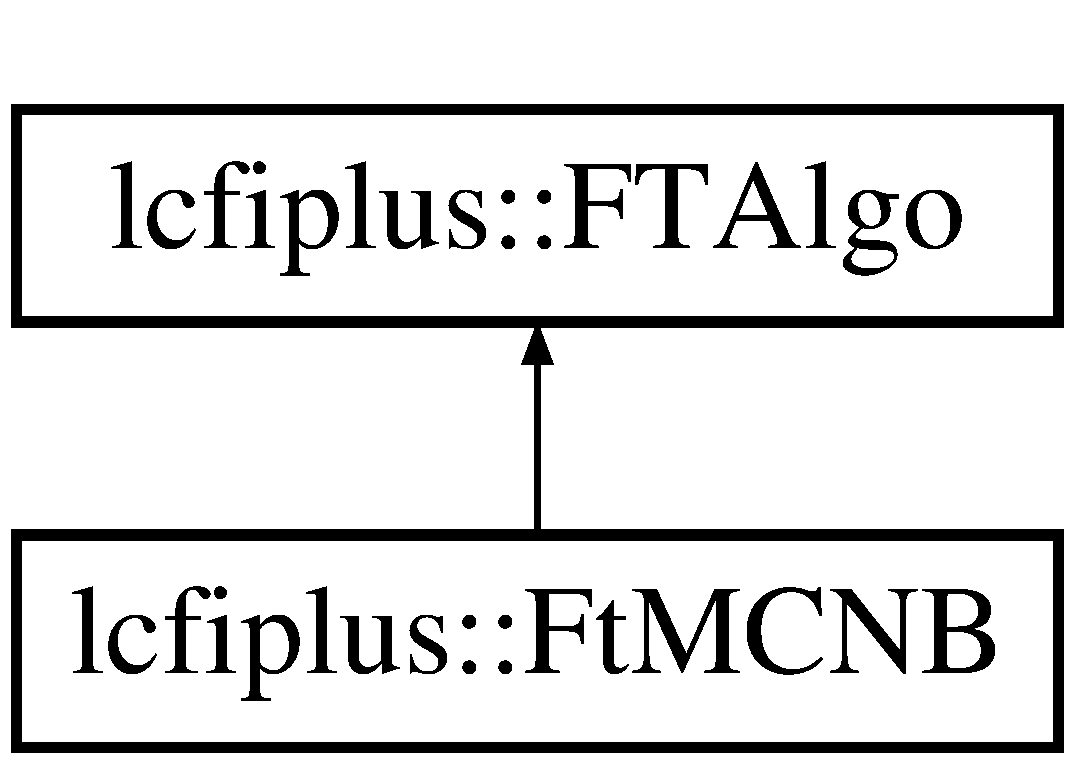
\includegraphics[height=2.000000cm]{classlcfiplus_1_1FtMCNB}
\end{center}
\end{figure}
\subsection*{Public Member Functions}
\begin{DoxyCompactItemize}
\item 
{\bf Ft\-M\-C\-N\-B} ()
\item 
void {\bf process\-Event} ()
\item 
void {\bf process} ()
\end{DoxyCompactItemize}
\subsection*{Additional Inherited Members}


\subsection{Constructor \& Destructor Documentation}
\index{lcfiplus\-::\-Ft\-M\-C\-N\-B@{lcfiplus\-::\-Ft\-M\-C\-N\-B}!Ft\-M\-C\-N\-B@{Ft\-M\-C\-N\-B}}
\index{Ft\-M\-C\-N\-B@{Ft\-M\-C\-N\-B}!lcfiplus::FtMCNB@{lcfiplus\-::\-Ft\-M\-C\-N\-B}}
\subsubsection[{Ft\-M\-C\-N\-B}]{\setlength{\rightskip}{0pt plus 5cm}lcfiplus\-::\-Ft\-M\-C\-N\-B\-::\-Ft\-M\-C\-N\-B (
\begin{DoxyParamCaption}
{}
\end{DoxyParamCaption}
)\hspace{0.3cm}{\ttfamily [inline]}}\label{classlcfiplus_1_1FtMCNB_a052f25ec7a5650bd383e40a6960e7614}


\subsection{Member Function Documentation}
\index{lcfiplus\-::\-Ft\-M\-C\-N\-B@{lcfiplus\-::\-Ft\-M\-C\-N\-B}!process@{process}}
\index{process@{process}!lcfiplus::FtMCNB@{lcfiplus\-::\-Ft\-M\-C\-N\-B}}
\subsubsection[{process}]{\setlength{\rightskip}{0pt plus 5cm}void lcfiplus\-::\-Ft\-M\-C\-N\-B\-::process (
\begin{DoxyParamCaption}
{}
\end{DoxyParamCaption}
)\hspace{0.3cm}{\ttfamily [inline]}, {\ttfamily [virtual]}}\label{classlcfiplus_1_1FtMCNB_a8495a07421105a91a8fc8f437e7f7e41}


Reimplemented from {\bf lcfiplus\-::\-F\-T\-Algo} \doxyref{}{p.}{classlcfiplus_1_1FTAlgo_a23cc3f3cd1c100ab6b5e16056112351a}.



References lcfiplus\-::\-M\-C\-Particle\-::get\-Daughters(), lcfiplus\-::\-M\-C\-Particle\-::get\-Semi\-Stable\-B\-Parent(), and lcfiplus\-::\-M\-C\-Particle\-::is\-Parent().

\index{lcfiplus\-::\-Ft\-M\-C\-N\-B@{lcfiplus\-::\-Ft\-M\-C\-N\-B}!process\-Event@{process\-Event}}
\index{process\-Event@{process\-Event}!lcfiplus::FtMCNB@{lcfiplus\-::\-Ft\-M\-C\-N\-B}}
\subsubsection[{process\-Event}]{\setlength{\rightskip}{0pt plus 5cm}void lcfiplus\-::\-Ft\-M\-C\-N\-B\-::process\-Event (
\begin{DoxyParamCaption}
{}
\end{DoxyParamCaption}
)\hspace{0.3cm}{\ttfamily [inline]}, {\ttfamily [virtual]}}\label{classlcfiplus_1_1FtMCNB_a98f262af3450b8f201bb1ae24dcf5a93}


Reimplemented from {\bf lcfiplus\-::\-F\-T\-Algo} \doxyref{}{p.}{classlcfiplus_1_1FTAlgo_a4b22a0cc29f4dc2045ba2770ab30a128}.



References lcfiplus\-::\-Vertex\-Finder\-Perfect\-::find\-Perfect\-Vertices().



The documentation for this class was generated from the following file\-:\begin{DoxyCompactItemize}
\item 
{\bf Flavor\-Tag.\-cc}\end{DoxyCompactItemize}

\section{lcfiplus\-:\-:Ft\-M\-C\-N\-C Class Reference}
\label{classlcfiplus_1_1FtMCNC}\index{lcfiplus\-::\-Ft\-M\-C\-N\-C@{lcfiplus\-::\-Ft\-M\-C\-N\-C}}
Inheritance diagram for lcfiplus\-:\-:Ft\-M\-C\-N\-C\-:\begin{figure}[H]
\begin{center}
\leavevmode
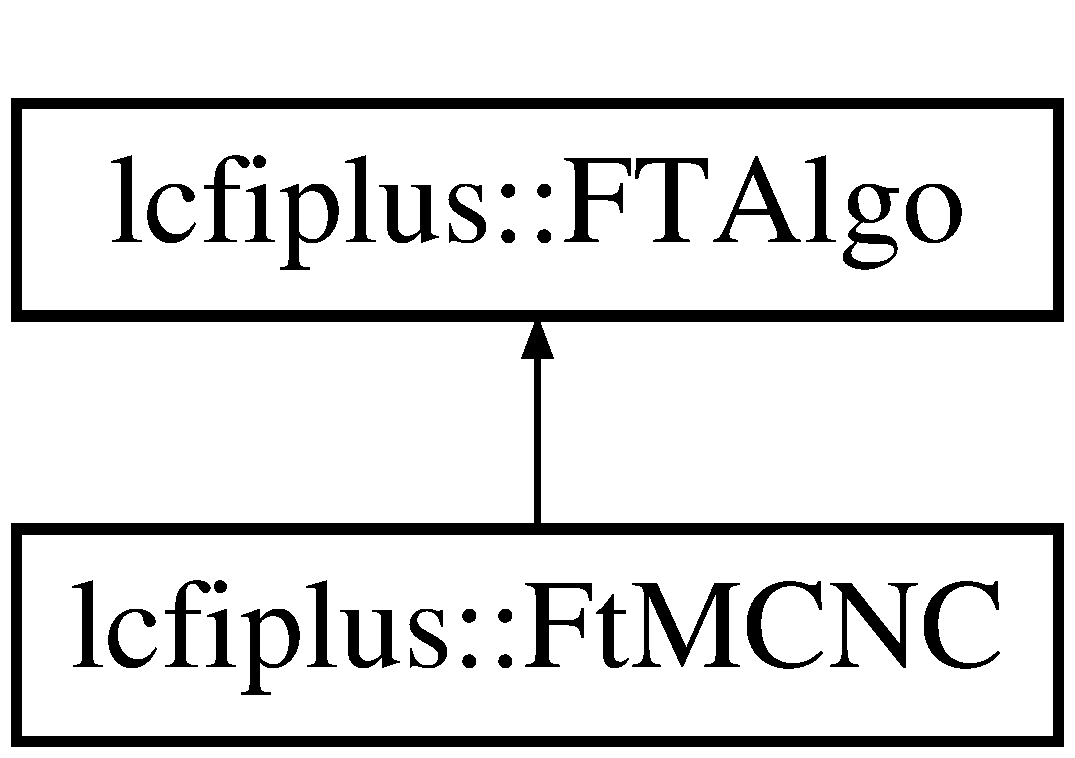
\includegraphics[height=2.000000cm]{classlcfiplus_1_1FtMCNC}
\end{center}
\end{figure}
\subsection*{Public Member Functions}
\begin{DoxyCompactItemize}
\item 
{\bf Ft\-M\-C\-N\-C} ()
\item 
void {\bf process\-Event} ()
\item 
void {\bf process} ()
\end{DoxyCompactItemize}
\subsection*{Additional Inherited Members}


\subsection{Constructor \& Destructor Documentation}
\index{lcfiplus\-::\-Ft\-M\-C\-N\-C@{lcfiplus\-::\-Ft\-M\-C\-N\-C}!Ft\-M\-C\-N\-C@{Ft\-M\-C\-N\-C}}
\index{Ft\-M\-C\-N\-C@{Ft\-M\-C\-N\-C}!lcfiplus::FtMCNC@{lcfiplus\-::\-Ft\-M\-C\-N\-C}}
\subsubsection[{Ft\-M\-C\-N\-C}]{\setlength{\rightskip}{0pt plus 5cm}lcfiplus\-::\-Ft\-M\-C\-N\-C\-::\-Ft\-M\-C\-N\-C (
\begin{DoxyParamCaption}
{}
\end{DoxyParamCaption}
)\hspace{0.3cm}{\ttfamily [inline]}}\label{classlcfiplus_1_1FtMCNC_a115d9ae4c179920ae8669c8724ee2b0f}


\subsection{Member Function Documentation}
\index{lcfiplus\-::\-Ft\-M\-C\-N\-C@{lcfiplus\-::\-Ft\-M\-C\-N\-C}!process@{process}}
\index{process@{process}!lcfiplus::FtMCNC@{lcfiplus\-::\-Ft\-M\-C\-N\-C}}
\subsubsection[{process}]{\setlength{\rightskip}{0pt plus 5cm}void lcfiplus\-::\-Ft\-M\-C\-N\-C\-::process (
\begin{DoxyParamCaption}
{}
\end{DoxyParamCaption}
)\hspace{0.3cm}{\ttfamily [inline]}, {\ttfamily [virtual]}}\label{classlcfiplus_1_1FtMCNC_a8832b03425cdc9fc1713c209587d3a20}


Reimplemented from {\bf lcfiplus\-::\-F\-T\-Algo} \doxyref{}{p.}{classlcfiplus_1_1FTAlgo_a23cc3f3cd1c100ab6b5e16056112351a}.



References lcfiplus\-::\-M\-C\-Particle\-::get\-Daughters(), lcfiplus\-::\-M\-C\-Particle\-::get\-Semi\-Stable\-B\-Parent(), lcfiplus\-::\-M\-C\-Particle\-::get\-Semi\-Stable\-C\-Parent(), and lcfiplus\-::\-M\-C\-Particle\-::is\-Parent().

\index{lcfiplus\-::\-Ft\-M\-C\-N\-C@{lcfiplus\-::\-Ft\-M\-C\-N\-C}!process\-Event@{process\-Event}}
\index{process\-Event@{process\-Event}!lcfiplus::FtMCNC@{lcfiplus\-::\-Ft\-M\-C\-N\-C}}
\subsubsection[{process\-Event}]{\setlength{\rightskip}{0pt plus 5cm}void lcfiplus\-::\-Ft\-M\-C\-N\-C\-::process\-Event (
\begin{DoxyParamCaption}
{}
\end{DoxyParamCaption}
)\hspace{0.3cm}{\ttfamily [inline]}, {\ttfamily [virtual]}}\label{classlcfiplus_1_1FtMCNC_af577b1bad0f22f3ad28db551534a455a}


Reimplemented from {\bf lcfiplus\-::\-F\-T\-Algo} \doxyref{}{p.}{classlcfiplus_1_1FTAlgo_a4b22a0cc29f4dc2045ba2770ab30a128}.



References lcfiplus\-::\-Vertex\-Finder\-Perfect\-::find\-Perfect\-Vertices().



The documentation for this class was generated from the following file\-:\begin{DoxyCompactItemize}
\item 
{\bf Flavor\-Tag.\-cc}\end{DoxyCompactItemize}

\section{lcfiplus\-:\-:Ft\-M\-C\-N\-Electron Class Reference}
\label{classlcfiplus_1_1FtMCNElectron}\index{lcfiplus\-::\-Ft\-M\-C\-N\-Electron@{lcfiplus\-::\-Ft\-M\-C\-N\-Electron}}
Inheritance diagram for lcfiplus\-:\-:Ft\-M\-C\-N\-Electron\-:\begin{figure}[H]
\begin{center}
\leavevmode
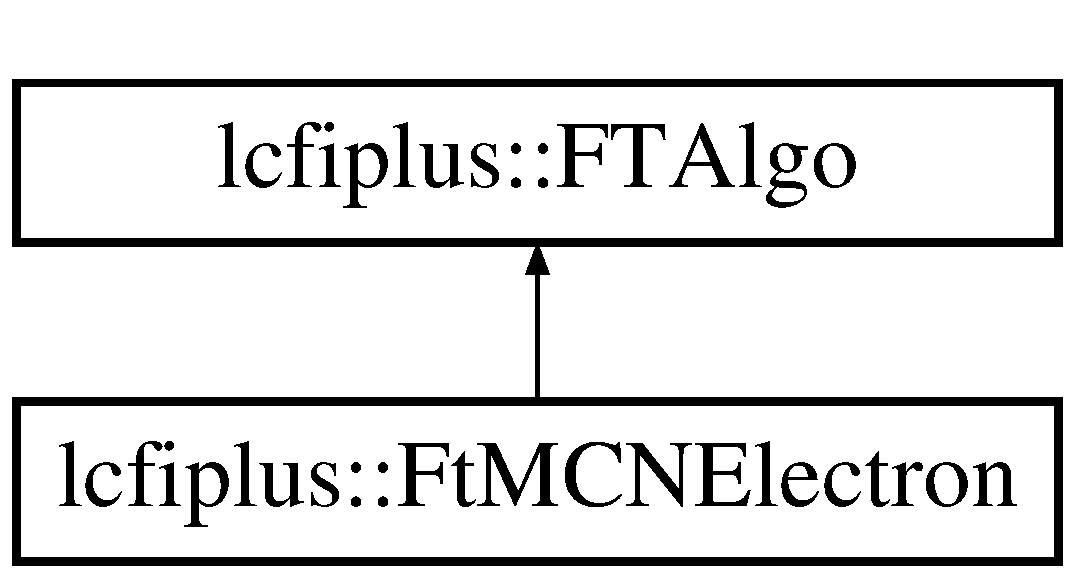
\includegraphics[height=2.000000cm]{classlcfiplus_1_1FtMCNElectron}
\end{center}
\end{figure}
\subsection*{Public Member Functions}
\begin{DoxyCompactItemize}
\item 
{\bf Ft\-M\-C\-N\-Electron} ()
\item 
void {\bf process} ()
\end{DoxyCompactItemize}
\subsection*{Additional Inherited Members}


\subsection{Constructor \& Destructor Documentation}
\index{lcfiplus\-::\-Ft\-M\-C\-N\-Electron@{lcfiplus\-::\-Ft\-M\-C\-N\-Electron}!Ft\-M\-C\-N\-Electron@{Ft\-M\-C\-N\-Electron}}
\index{Ft\-M\-C\-N\-Electron@{Ft\-M\-C\-N\-Electron}!lcfiplus::FtMCNElectron@{lcfiplus\-::\-Ft\-M\-C\-N\-Electron}}
\subsubsection[{Ft\-M\-C\-N\-Electron}]{\setlength{\rightskip}{0pt plus 5cm}lcfiplus\-::\-Ft\-M\-C\-N\-Electron\-::\-Ft\-M\-C\-N\-Electron (
\begin{DoxyParamCaption}
{}
\end{DoxyParamCaption}
)\hspace{0.3cm}{\ttfamily [inline]}}\label{classlcfiplus_1_1FtMCNElectron_a9b67bf5d2835939b70aabc01c4060c9c}


\subsection{Member Function Documentation}
\index{lcfiplus\-::\-Ft\-M\-C\-N\-Electron@{lcfiplus\-::\-Ft\-M\-C\-N\-Electron}!process@{process}}
\index{process@{process}!lcfiplus::FtMCNElectron@{lcfiplus\-::\-Ft\-M\-C\-N\-Electron}}
\subsubsection[{process}]{\setlength{\rightskip}{0pt plus 5cm}void lcfiplus\-::\-Ft\-M\-C\-N\-Electron\-::process (
\begin{DoxyParamCaption}
{}
\end{DoxyParamCaption}
)\hspace{0.3cm}{\ttfamily [inline]}, {\ttfamily [virtual]}}\label{classlcfiplus_1_1FtMCNElectron_aa6883f0b241486acdae416e06f5c8d14}


Reimplemented from {\bf lcfiplus\-::\-F\-T\-Algo} \doxyref{}{p.}{classlcfiplus_1_1FTAlgo_a23cc3f3cd1c100ab6b5e16056112351a}.



The documentation for this class was generated from the following file\-:\begin{DoxyCompactItemize}
\item 
{\bf Flavor\-Tag.\-cc}\end{DoxyCompactItemize}

\section{lcfiplus\-:\-:Ft\-M\-C\-N\-Muon Class Reference}
\label{classlcfiplus_1_1FtMCNMuon}\index{lcfiplus\-::\-Ft\-M\-C\-N\-Muon@{lcfiplus\-::\-Ft\-M\-C\-N\-Muon}}
Inheritance diagram for lcfiplus\-:\-:Ft\-M\-C\-N\-Muon\-:\begin{figure}[H]
\begin{center}
\leavevmode
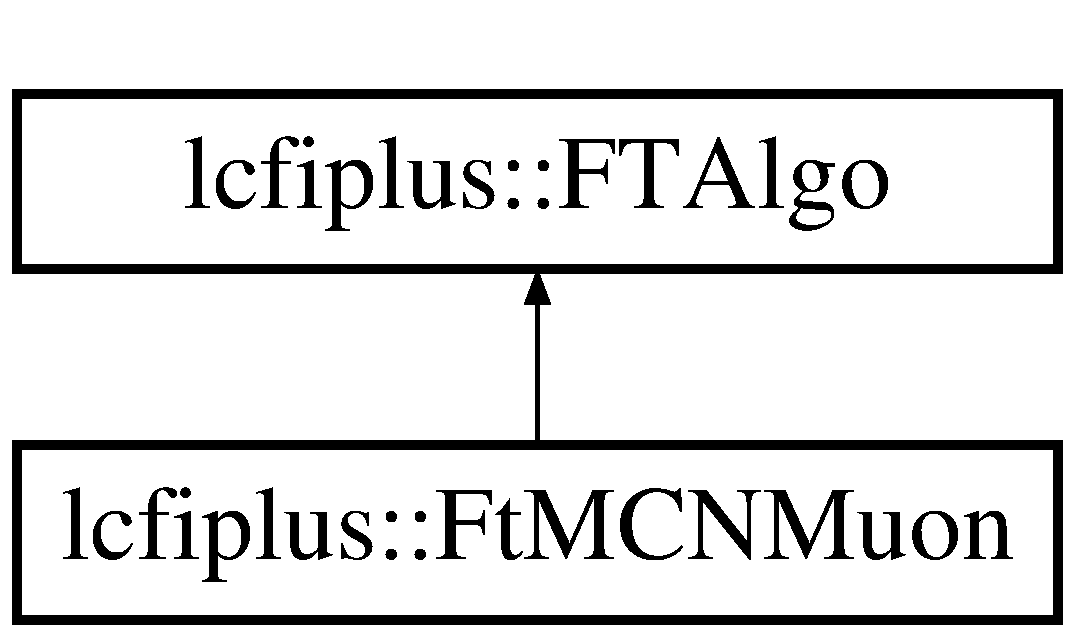
\includegraphics[height=2.000000cm]{classlcfiplus_1_1FtMCNMuon}
\end{center}
\end{figure}
\subsection*{Public Member Functions}
\begin{DoxyCompactItemize}
\item 
{\bf Ft\-M\-C\-N\-Muon} ()
\item 
void {\bf process} ()
\end{DoxyCompactItemize}
\subsection*{Additional Inherited Members}


\subsection{Constructor \& Destructor Documentation}
\index{lcfiplus\-::\-Ft\-M\-C\-N\-Muon@{lcfiplus\-::\-Ft\-M\-C\-N\-Muon}!Ft\-M\-C\-N\-Muon@{Ft\-M\-C\-N\-Muon}}
\index{Ft\-M\-C\-N\-Muon@{Ft\-M\-C\-N\-Muon}!lcfiplus::FtMCNMuon@{lcfiplus\-::\-Ft\-M\-C\-N\-Muon}}
\subsubsection[{Ft\-M\-C\-N\-Muon}]{\setlength{\rightskip}{0pt plus 5cm}lcfiplus\-::\-Ft\-M\-C\-N\-Muon\-::\-Ft\-M\-C\-N\-Muon (
\begin{DoxyParamCaption}
{}
\end{DoxyParamCaption}
)\hspace{0.3cm}{\ttfamily [inline]}}\label{classlcfiplus_1_1FtMCNMuon_ac4e90d9bb6bc7b05358b06ca5c48fb33}


\subsection{Member Function Documentation}
\index{lcfiplus\-::\-Ft\-M\-C\-N\-Muon@{lcfiplus\-::\-Ft\-M\-C\-N\-Muon}!process@{process}}
\index{process@{process}!lcfiplus::FtMCNMuon@{lcfiplus\-::\-Ft\-M\-C\-N\-Muon}}
\subsubsection[{process}]{\setlength{\rightskip}{0pt plus 5cm}void lcfiplus\-::\-Ft\-M\-C\-N\-Muon\-::process (
\begin{DoxyParamCaption}
{}
\end{DoxyParamCaption}
)\hspace{0.3cm}{\ttfamily [inline]}, {\ttfamily [virtual]}}\label{classlcfiplus_1_1FtMCNMuon_a257089c0418ddb5bad6d4f644462b98c}


Reimplemented from {\bf lcfiplus\-::\-F\-T\-Algo} \doxyref{}{p.}{classlcfiplus_1_1FTAlgo_a23cc3f3cd1c100ab6b5e16056112351a}.



The documentation for this class was generated from the following file\-:\begin{DoxyCompactItemize}
\item 
{\bf Flavor\-Tag.\-cc}\end{DoxyCompactItemize}

\section{lcfiplus\-:\-:Ft\-N\-B\-Ness Class Reference}
\label{classlcfiplus_1_1FtNBNess}\index{lcfiplus\-::\-Ft\-N\-B\-Ness@{lcfiplus\-::\-Ft\-N\-B\-Ness}}
Inheritance diagram for lcfiplus\-:\-:Ft\-N\-B\-Ness\-:\begin{figure}[H]
\begin{center}
\leavevmode
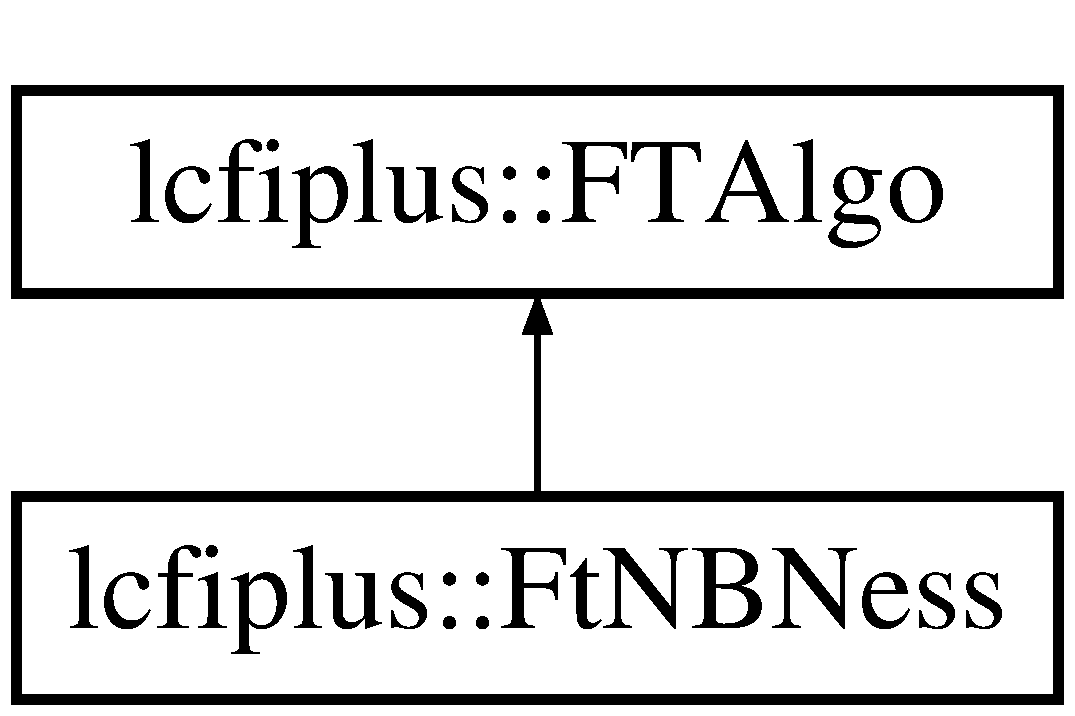
\includegraphics[height=2.000000cm]{classlcfiplus_1_1FtNBNess}
\end{center}
\end{figure}
\subsection*{Public Member Functions}
\begin{DoxyCompactItemize}
\item 
{\bf Ft\-N\-B\-Ness} ()
\item 
void {\bf process} ()
\end{DoxyCompactItemize}
\subsection*{Additional Inherited Members}


\subsection{Constructor \& Destructor Documentation}
\index{lcfiplus\-::\-Ft\-N\-B\-Ness@{lcfiplus\-::\-Ft\-N\-B\-Ness}!Ft\-N\-B\-Ness@{Ft\-N\-B\-Ness}}
\index{Ft\-N\-B\-Ness@{Ft\-N\-B\-Ness}!lcfiplus::FtNBNess@{lcfiplus\-::\-Ft\-N\-B\-Ness}}
\subsubsection[{Ft\-N\-B\-Ness}]{\setlength{\rightskip}{0pt plus 5cm}lcfiplus\-::\-Ft\-N\-B\-Ness\-::\-Ft\-N\-B\-Ness (
\begin{DoxyParamCaption}
{}
\end{DoxyParamCaption}
)\hspace{0.3cm}{\ttfamily [inline]}}\label{classlcfiplus_1_1FtNBNess_a225f9809c7db3d1fa661b4ce84f3dbfb}


\subsection{Member Function Documentation}
\index{lcfiplus\-::\-Ft\-N\-B\-Ness@{lcfiplus\-::\-Ft\-N\-B\-Ness}!process@{process}}
\index{process@{process}!lcfiplus::FtNBNess@{lcfiplus\-::\-Ft\-N\-B\-Ness}}
\subsubsection[{process}]{\setlength{\rightskip}{0pt plus 5cm}void lcfiplus\-::\-Ft\-N\-B\-Ness\-::process (
\begin{DoxyParamCaption}
{}
\end{DoxyParamCaption}
)\hspace{0.3cm}{\ttfamily [inline]}, {\ttfamily [virtual]}}\label{classlcfiplus_1_1FtNBNess_af9a1114a1d0f001a10036490570e5a82}


Reimplemented from {\bf lcfiplus\-::\-F\-T\-Algo} \doxyref{}{p.}{classlcfiplus_1_1FTAlgo_a23cc3f3cd1c100ab6b5e16056112351a}.



The documentation for this class was generated from the following file\-:\begin{DoxyCompactItemize}
\item 
{\bf Flavor\-Tag.\-cc}\end{DoxyCompactItemize}

\section{lcfiplus\-:\-:Ft\-N\-Electron Class Reference}
\label{classlcfiplus_1_1FtNElectron}\index{lcfiplus\-::\-Ft\-N\-Electron@{lcfiplus\-::\-Ft\-N\-Electron}}
Inheritance diagram for lcfiplus\-:\-:Ft\-N\-Electron\-:\begin{figure}[H]
\begin{center}
\leavevmode
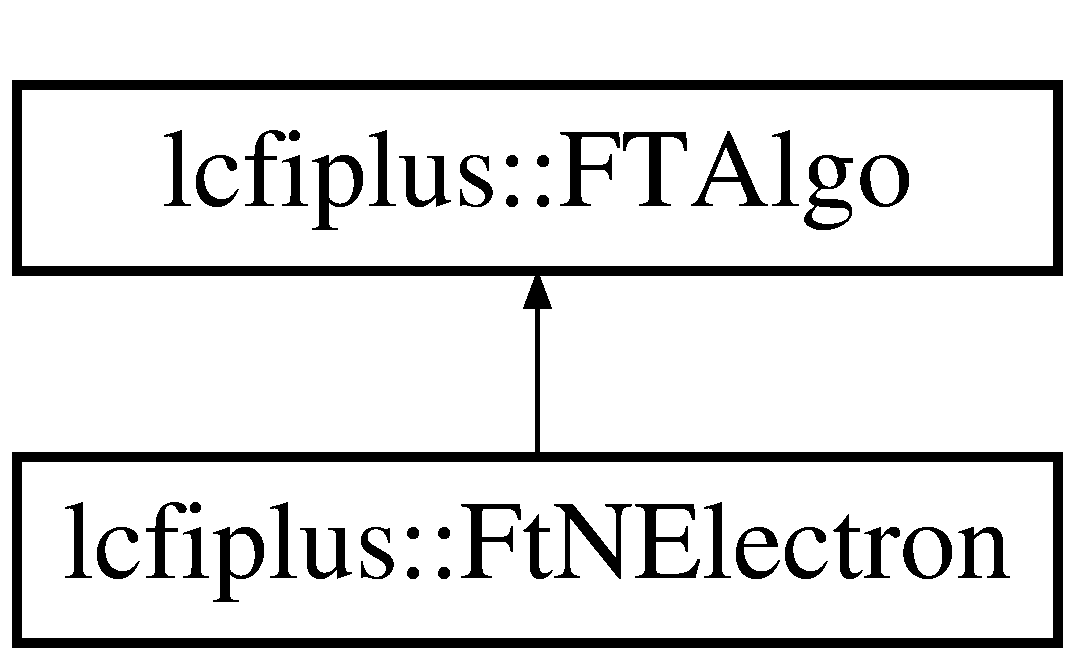
\includegraphics[height=2.000000cm]{classlcfiplus_1_1FtNElectron}
\end{center}
\end{figure}
\subsection*{Public Member Functions}
\begin{DoxyCompactItemize}
\item 
{\bf Ft\-N\-Electron} (bool usevt)
\item 
void {\bf process} ()
\end{DoxyCompactItemize}
\subsection*{Additional Inherited Members}


\subsection{Constructor \& Destructor Documentation}
\index{lcfiplus\-::\-Ft\-N\-Electron@{lcfiplus\-::\-Ft\-N\-Electron}!Ft\-N\-Electron@{Ft\-N\-Electron}}
\index{Ft\-N\-Electron@{Ft\-N\-Electron}!lcfiplus::FtNElectron@{lcfiplus\-::\-Ft\-N\-Electron}}
\subsubsection[{Ft\-N\-Electron}]{\setlength{\rightskip}{0pt plus 5cm}lcfiplus\-::\-Ft\-N\-Electron\-::\-Ft\-N\-Electron (
\begin{DoxyParamCaption}
\item[{bool}]{usevt}
\end{DoxyParamCaption}
)\hspace{0.3cm}{\ttfamily [inline]}}\label{classlcfiplus_1_1FtNElectron_a427f4f8e81f44a9dcbe3150368252381}


\subsection{Member Function Documentation}
\index{lcfiplus\-::\-Ft\-N\-Electron@{lcfiplus\-::\-Ft\-N\-Electron}!process@{process}}
\index{process@{process}!lcfiplus::FtNElectron@{lcfiplus\-::\-Ft\-N\-Electron}}
\subsubsection[{process}]{\setlength{\rightskip}{0pt plus 5cm}void lcfiplus\-::\-Ft\-N\-Electron\-::process (
\begin{DoxyParamCaption}
{}
\end{DoxyParamCaption}
)\hspace{0.3cm}{\ttfamily [inline]}, {\ttfamily [virtual]}}\label{classlcfiplus_1_1FtNElectron_a2beafefb58d803a1af565c11f301eab8}


Reimplemented from {\bf lcfiplus\-::\-F\-T\-Algo} \doxyref{}{p.}{classlcfiplus_1_1FTAlgo_a23cc3f3cd1c100ab6b5e16056112351a}.



References lcfiplus\-::algo\-Etc\-::\-Simple\-Sec\-Electron\-Finder().



The documentation for this class was generated from the following file\-:\begin{DoxyCompactItemize}
\item 
{\bf Flavor\-Tag.\-cc}\end{DoxyCompactItemize}

\section{lcfiplus\-:\-:Ft\-N\-Electron\-P\-I\-D Class Reference}
\label{classlcfiplus_1_1FtNElectronPID}\index{lcfiplus\-::\-Ft\-N\-Electron\-P\-I\-D@{lcfiplus\-::\-Ft\-N\-Electron\-P\-I\-D}}
Inheritance diagram for lcfiplus\-:\-:Ft\-N\-Electron\-P\-I\-D\-:\begin{figure}[H]
\begin{center}
\leavevmode
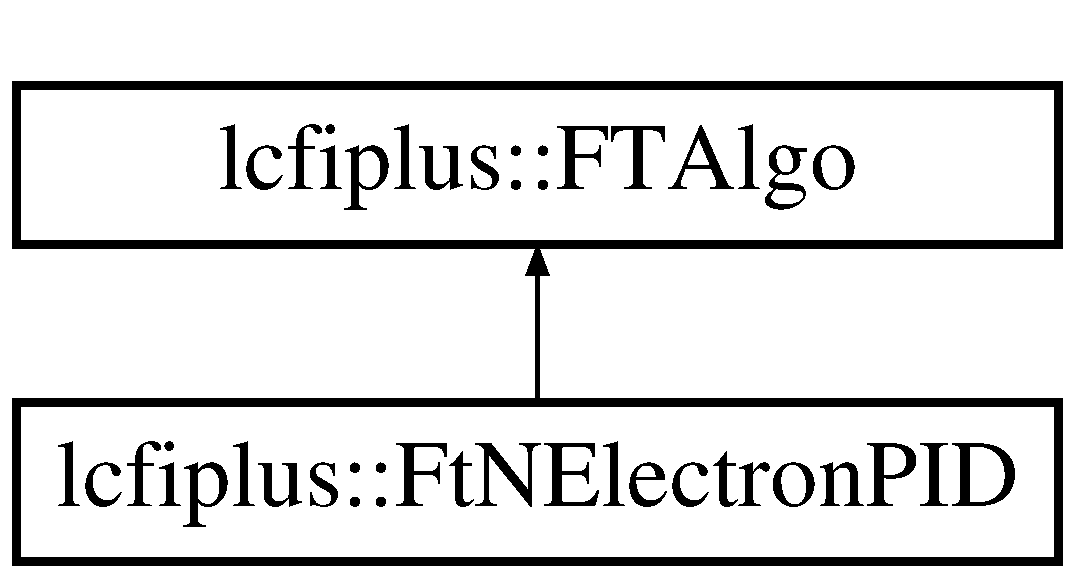
\includegraphics[height=2.000000cm]{classlcfiplus_1_1FtNElectronPID}
\end{center}
\end{figure}
\subsection*{Public Member Functions}
\begin{DoxyCompactItemize}
\item 
{\bf Ft\-N\-Electron\-P\-I\-D} (bool usevt)
\item 
void {\bf process} ()
\end{DoxyCompactItemize}
\subsection*{Additional Inherited Members}


\subsection{Constructor \& Destructor Documentation}
\index{lcfiplus\-::\-Ft\-N\-Electron\-P\-I\-D@{lcfiplus\-::\-Ft\-N\-Electron\-P\-I\-D}!Ft\-N\-Electron\-P\-I\-D@{Ft\-N\-Electron\-P\-I\-D}}
\index{Ft\-N\-Electron\-P\-I\-D@{Ft\-N\-Electron\-P\-I\-D}!lcfiplus::FtNElectronPID@{lcfiplus\-::\-Ft\-N\-Electron\-P\-I\-D}}
\subsubsection[{Ft\-N\-Electron\-P\-I\-D}]{\setlength{\rightskip}{0pt plus 5cm}lcfiplus\-::\-Ft\-N\-Electron\-P\-I\-D\-::\-Ft\-N\-Electron\-P\-I\-D (
\begin{DoxyParamCaption}
\item[{bool}]{usevt}
\end{DoxyParamCaption}
)\hspace{0.3cm}{\ttfamily [inline]}}\label{classlcfiplus_1_1FtNElectronPID_ade16e60c2d5201bd101ca89c26d93b03}


\subsection{Member Function Documentation}
\index{lcfiplus\-::\-Ft\-N\-Electron\-P\-I\-D@{lcfiplus\-::\-Ft\-N\-Electron\-P\-I\-D}!process@{process}}
\index{process@{process}!lcfiplus::FtNElectronPID@{lcfiplus\-::\-Ft\-N\-Electron\-P\-I\-D}}
\subsubsection[{process}]{\setlength{\rightskip}{0pt plus 5cm}void lcfiplus\-::\-Ft\-N\-Electron\-P\-I\-D\-::process (
\begin{DoxyParamCaption}
{}
\end{DoxyParamCaption}
)\hspace{0.3cm}{\ttfamily [inline]}, {\ttfamily [virtual]}}\label{classlcfiplus_1_1FtNElectronPID_a6b4cb272635b48c13c3acd2810cab715}


Reimplemented from {\bf lcfiplus\-::\-F\-T\-Algo} \doxyref{}{p.}{classlcfiplus_1_1FTAlgo_a23cc3f3cd1c100ab6b5e16056112351a}.



The documentation for this class was generated from the following file\-:\begin{DoxyCompactItemize}
\item 
{\bf Flavor\-Tag.\-cc}\end{DoxyCompactItemize}

\section{lcfiplus\-:\-:Ft\-N\-Muon Class Reference}
\label{classlcfiplus_1_1FtNMuon}\index{lcfiplus\-::\-Ft\-N\-Muon@{lcfiplus\-::\-Ft\-N\-Muon}}
Inheritance diagram for lcfiplus\-:\-:Ft\-N\-Muon\-:\begin{figure}[H]
\begin{center}
\leavevmode
\includegraphics[height=2.000000cm]{classlcfiplus_1_1FtNMuon}
\end{center}
\end{figure}
\subsection*{Public Member Functions}
\begin{DoxyCompactItemize}
\item 
{\bf Ft\-N\-Muon} (bool usevt)
\item 
void {\bf process} ()
\end{DoxyCompactItemize}
\subsection*{Additional Inherited Members}


\subsection{Constructor \& Destructor Documentation}
\index{lcfiplus\-::\-Ft\-N\-Muon@{lcfiplus\-::\-Ft\-N\-Muon}!Ft\-N\-Muon@{Ft\-N\-Muon}}
\index{Ft\-N\-Muon@{Ft\-N\-Muon}!lcfiplus::FtNMuon@{lcfiplus\-::\-Ft\-N\-Muon}}
\subsubsection[{Ft\-N\-Muon}]{\setlength{\rightskip}{0pt plus 5cm}lcfiplus\-::\-Ft\-N\-Muon\-::\-Ft\-N\-Muon (
\begin{DoxyParamCaption}
\item[{bool}]{usevt}
\end{DoxyParamCaption}
)\hspace{0.3cm}{\ttfamily [inline]}}\label{classlcfiplus_1_1FtNMuon_a39cc6ac09f3641d2bb271748c429032a}


\subsection{Member Function Documentation}
\index{lcfiplus\-::\-Ft\-N\-Muon@{lcfiplus\-::\-Ft\-N\-Muon}!process@{process}}
\index{process@{process}!lcfiplus::FtNMuon@{lcfiplus\-::\-Ft\-N\-Muon}}
\subsubsection[{process}]{\setlength{\rightskip}{0pt plus 5cm}void lcfiplus\-::\-Ft\-N\-Muon\-::process (
\begin{DoxyParamCaption}
{}
\end{DoxyParamCaption}
)\hspace{0.3cm}{\ttfamily [inline]}, {\ttfamily [virtual]}}\label{classlcfiplus_1_1FtNMuon_adc2c58022919b1732aa130148e4ee068}


Reimplemented from {\bf lcfiplus\-::\-F\-T\-Algo} \doxyref{}{p.}{classlcfiplus_1_1FTAlgo_a23cc3f3cd1c100ab6b5e16056112351a}.



References lcfiplus\-::algo\-Etc\-::\-Simple\-Sec\-Muon\-Finder().



The documentation for this class was generated from the following file\-:\begin{DoxyCompactItemize}
\item 
{\bf Flavor\-Tag.\-cc}\end{DoxyCompactItemize}

\section{lcfiplus\-:\-:Ft\-N\-Muon\-P\-I\-D Class Reference}
\label{classlcfiplus_1_1FtNMuonPID}\index{lcfiplus\-::\-Ft\-N\-Muon\-P\-I\-D@{lcfiplus\-::\-Ft\-N\-Muon\-P\-I\-D}}
Inheritance diagram for lcfiplus\-:\-:Ft\-N\-Muon\-P\-I\-D\-:\begin{figure}[H]
\begin{center}
\leavevmode
\includegraphics[height=2.000000cm]{classlcfiplus_1_1FtNMuonPID}
\end{center}
\end{figure}
\subsection*{Public Member Functions}
\begin{DoxyCompactItemize}
\item 
{\bf Ft\-N\-Muon\-P\-I\-D} (bool usevt)
\item 
void {\bf process} ()
\end{DoxyCompactItemize}
\subsection*{Additional Inherited Members}


\subsection{Constructor \& Destructor Documentation}
\index{lcfiplus\-::\-Ft\-N\-Muon\-P\-I\-D@{lcfiplus\-::\-Ft\-N\-Muon\-P\-I\-D}!Ft\-N\-Muon\-P\-I\-D@{Ft\-N\-Muon\-P\-I\-D}}
\index{Ft\-N\-Muon\-P\-I\-D@{Ft\-N\-Muon\-P\-I\-D}!lcfiplus::FtNMuonPID@{lcfiplus\-::\-Ft\-N\-Muon\-P\-I\-D}}
\subsubsection[{Ft\-N\-Muon\-P\-I\-D}]{\setlength{\rightskip}{0pt plus 5cm}lcfiplus\-::\-Ft\-N\-Muon\-P\-I\-D\-::\-Ft\-N\-Muon\-P\-I\-D (
\begin{DoxyParamCaption}
\item[{bool}]{usevt}
\end{DoxyParamCaption}
)\hspace{0.3cm}{\ttfamily [inline]}}\label{classlcfiplus_1_1FtNMuonPID_ae9887f4d109a5314b949a163a3b12084}


\subsection{Member Function Documentation}
\index{lcfiplus\-::\-Ft\-N\-Muon\-P\-I\-D@{lcfiplus\-::\-Ft\-N\-Muon\-P\-I\-D}!process@{process}}
\index{process@{process}!lcfiplus::FtNMuonPID@{lcfiplus\-::\-Ft\-N\-Muon\-P\-I\-D}}
\subsubsection[{process}]{\setlength{\rightskip}{0pt plus 5cm}void lcfiplus\-::\-Ft\-N\-Muon\-P\-I\-D\-::process (
\begin{DoxyParamCaption}
{}
\end{DoxyParamCaption}
)\hspace{0.3cm}{\ttfamily [inline]}, {\ttfamily [virtual]}}\label{classlcfiplus_1_1FtNMuonPID_aa11ced9d3f89b6046206df1fb3ef879e}


Reimplemented from {\bf lcfiplus\-::\-F\-T\-Algo} \doxyref{}{p.}{classlcfiplus_1_1FTAlgo_a23cc3f3cd1c100ab6b5e16056112351a}.



The documentation for this class was generated from the following file\-:\begin{DoxyCompactItemize}
\item 
{\bf Flavor\-Tag.\-cc}\end{DoxyCompactItemize}

\section{lcfiplus\-:\-:Ft\-N\-Pi0s1 Class Reference}
\label{classlcfiplus_1_1FtNPi0s1}\index{lcfiplus\-::\-Ft\-N\-Pi0s1@{lcfiplus\-::\-Ft\-N\-Pi0s1}}
Inheritance diagram for lcfiplus\-:\-:Ft\-N\-Pi0s1\-:\begin{figure}[H]
\begin{center}
\leavevmode
\includegraphics[height=2.000000cm]{classlcfiplus_1_1FtNPi0s1}
\end{center}
\end{figure}
\subsection*{Public Member Functions}
\begin{DoxyCompactItemize}
\item 
{\bf Ft\-N\-Pi0s1} ()
\item 
void {\bf process} ()
\end{DoxyCompactItemize}
\subsection*{Additional Inherited Members}


\subsection{Constructor \& Destructor Documentation}
\index{lcfiplus\-::\-Ft\-N\-Pi0s1@{lcfiplus\-::\-Ft\-N\-Pi0s1}!Ft\-N\-Pi0s1@{Ft\-N\-Pi0s1}}
\index{Ft\-N\-Pi0s1@{Ft\-N\-Pi0s1}!lcfiplus::FtNPi0s1@{lcfiplus\-::\-Ft\-N\-Pi0s1}}
\subsubsection[{Ft\-N\-Pi0s1}]{\setlength{\rightskip}{0pt plus 5cm}lcfiplus\-::\-Ft\-N\-Pi0s1\-::\-Ft\-N\-Pi0s1 (
\begin{DoxyParamCaption}
{}
\end{DoxyParamCaption}
)\hspace{0.3cm}{\ttfamily [inline]}}\label{classlcfiplus_1_1FtNPi0s1_aba83392a3dba6a3220a84fe78a26c07b}


\subsection{Member Function Documentation}
\index{lcfiplus\-::\-Ft\-N\-Pi0s1@{lcfiplus\-::\-Ft\-N\-Pi0s1}!process@{process}}
\index{process@{process}!lcfiplus::FtNPi0s1@{lcfiplus\-::\-Ft\-N\-Pi0s1}}
\subsubsection[{process}]{\setlength{\rightskip}{0pt plus 5cm}void lcfiplus\-::\-Ft\-N\-Pi0s1\-::process (
\begin{DoxyParamCaption}
{}
\end{DoxyParamCaption}
)\hspace{0.3cm}{\ttfamily [inline]}, {\ttfamily [virtual]}}\label{classlcfiplus_1_1FtNPi0s1_a7fdafff17efcbeabf1697488b99cbeae}


Reimplemented from {\bf lcfiplus\-::\-F\-T\-Algo} \doxyref{}{p.}{classlcfiplus_1_1FTAlgo_a23cc3f3cd1c100ab6b5e16056112351a}.



The documentation for this class was generated from the following file\-:\begin{DoxyCompactItemize}
\item 
{\bf Flavor\-Tag.\-cc}\end{DoxyCompactItemize}

\section{lcfiplus\-:\-:Ft\-N\-Pi0s2 Class Reference}
\label{classlcfiplus_1_1FtNPi0s2}\index{lcfiplus\-::\-Ft\-N\-Pi0s2@{lcfiplus\-::\-Ft\-N\-Pi0s2}}
Inheritance diagram for lcfiplus\-:\-:Ft\-N\-Pi0s2\-:\begin{figure}[H]
\begin{center}
\leavevmode
\includegraphics[height=2.000000cm]{classlcfiplus_1_1FtNPi0s2}
\end{center}
\end{figure}
\subsection*{Public Member Functions}
\begin{DoxyCompactItemize}
\item 
{\bf Ft\-N\-Pi0s2} ()
\item 
void {\bf process} ()
\end{DoxyCompactItemize}
\subsection*{Additional Inherited Members}


\subsection{Constructor \& Destructor Documentation}
\index{lcfiplus\-::\-Ft\-N\-Pi0s2@{lcfiplus\-::\-Ft\-N\-Pi0s2}!Ft\-N\-Pi0s2@{Ft\-N\-Pi0s2}}
\index{Ft\-N\-Pi0s2@{Ft\-N\-Pi0s2}!lcfiplus::FtNPi0s2@{lcfiplus\-::\-Ft\-N\-Pi0s2}}
\subsubsection[{Ft\-N\-Pi0s2}]{\setlength{\rightskip}{0pt plus 5cm}lcfiplus\-::\-Ft\-N\-Pi0s2\-::\-Ft\-N\-Pi0s2 (
\begin{DoxyParamCaption}
{}
\end{DoxyParamCaption}
)\hspace{0.3cm}{\ttfamily [inline]}}\label{classlcfiplus_1_1FtNPi0s2_a545a7a6f36e8fc0e48b9b5d170ee7af6}


\subsection{Member Function Documentation}
\index{lcfiplus\-::\-Ft\-N\-Pi0s2@{lcfiplus\-::\-Ft\-N\-Pi0s2}!process@{process}}
\index{process@{process}!lcfiplus::FtNPi0s2@{lcfiplus\-::\-Ft\-N\-Pi0s2}}
\subsubsection[{process}]{\setlength{\rightskip}{0pt plus 5cm}void lcfiplus\-::\-Ft\-N\-Pi0s2\-::process (
\begin{DoxyParamCaption}
{}
\end{DoxyParamCaption}
)\hspace{0.3cm}{\ttfamily [inline]}, {\ttfamily [virtual]}}\label{classlcfiplus_1_1FtNPi0s2_a924b3a544cab8451465c7d33e7480b87}


Reimplemented from {\bf lcfiplus\-::\-F\-T\-Algo} \doxyref{}{p.}{classlcfiplus_1_1FTAlgo_a23cc3f3cd1c100ab6b5e16056112351a}.



The documentation for this class was generated from the following file\-:\begin{DoxyCompactItemize}
\item 
{\bf Flavor\-Tag.\-cc}\end{DoxyCompactItemize}

\section{lcfiplus\-:\-:Ft\-N\-Sec\-Tracks Class Reference}
\label{classlcfiplus_1_1FtNSecTracks}\index{lcfiplus\-::\-Ft\-N\-Sec\-Tracks@{lcfiplus\-::\-Ft\-N\-Sec\-Tracks}}
Inheritance diagram for lcfiplus\-:\-:Ft\-N\-Sec\-Tracks\-:\begin{figure}[H]
\begin{center}
\leavevmode
\includegraphics[height=2.000000cm]{classlcfiplus_1_1FtNSecTracks}
\end{center}
\end{figure}
\subsection*{Public Member Functions}
\begin{DoxyCompactItemize}
\item 
{\bf Ft\-N\-Sec\-Tracks} (bool usevt)
\item 
void {\bf process} ()
\end{DoxyCompactItemize}
\subsection*{Additional Inherited Members}


\subsection{Constructor \& Destructor Documentation}
\index{lcfiplus\-::\-Ft\-N\-Sec\-Tracks@{lcfiplus\-::\-Ft\-N\-Sec\-Tracks}!Ft\-N\-Sec\-Tracks@{Ft\-N\-Sec\-Tracks}}
\index{Ft\-N\-Sec\-Tracks@{Ft\-N\-Sec\-Tracks}!lcfiplus::FtNSecTracks@{lcfiplus\-::\-Ft\-N\-Sec\-Tracks}}
\subsubsection[{Ft\-N\-Sec\-Tracks}]{\setlength{\rightskip}{0pt plus 5cm}lcfiplus\-::\-Ft\-N\-Sec\-Tracks\-::\-Ft\-N\-Sec\-Tracks (
\begin{DoxyParamCaption}
\item[{bool}]{usevt}
\end{DoxyParamCaption}
)\hspace{0.3cm}{\ttfamily [inline]}}\label{classlcfiplus_1_1FtNSecTracks_a40f72ee1e9233c6b136ebe2871bcab7d}


\subsection{Member Function Documentation}
\index{lcfiplus\-::\-Ft\-N\-Sec\-Tracks@{lcfiplus\-::\-Ft\-N\-Sec\-Tracks}!process@{process}}
\index{process@{process}!lcfiplus::FtNSecTracks@{lcfiplus\-::\-Ft\-N\-Sec\-Tracks}}
\subsubsection[{process}]{\setlength{\rightskip}{0pt plus 5cm}void lcfiplus\-::\-Ft\-N\-Sec\-Tracks\-::process (
\begin{DoxyParamCaption}
{}
\end{DoxyParamCaption}
)\hspace{0.3cm}{\ttfamily [inline]}, {\ttfamily [virtual]}}\label{classlcfiplus_1_1FtNSecTracks_aa83884b0ee9505e92f2051b1a925569a}


Reimplemented from {\bf lcfiplus\-::\-F\-T\-Algo} \doxyref{}{p.}{classlcfiplus_1_1FTAlgo_a23cc3f3cd1c100ab6b5e16056112351a}.



References lcfiplus\-::\-Track\-Selector\-Config\-::max\-D0, lcfiplus\-::\-Track\-Selector\-Config\-::max\-Z0, lcfiplus\-::\-Track\-Selector\-Config\-::min\-D0\-Sig, and lcfiplus\-::\-Track\-Selector\-Config\-::min\-Z0\-Sig.



The documentation for this class was generated from the following file\-:\begin{DoxyCompactItemize}
\item 
{\bf Flavor\-Tag.\-cc}\end{DoxyCompactItemize}

\section{lcfiplus\-:\-:Ft\-Ntrk Class Reference}
\label{classlcfiplus_1_1FtNtrk}\index{lcfiplus\-::\-Ft\-Ntrk@{lcfiplus\-::\-Ft\-Ntrk}}
Inheritance diagram for lcfiplus\-:\-:Ft\-Ntrk\-:\begin{figure}[H]
\begin{center}
\leavevmode
\includegraphics[height=2.000000cm]{classlcfiplus_1_1FtNtrk}
\end{center}
\end{figure}
\subsection*{Public Member Functions}
\begin{DoxyCompactItemize}
\item 
{\bf Ft\-Ntrk} ()
\item 
void {\bf process} ()
\end{DoxyCompactItemize}
\subsection*{Additional Inherited Members}


\subsection{Constructor \& Destructor Documentation}
\index{lcfiplus\-::\-Ft\-Ntrk@{lcfiplus\-::\-Ft\-Ntrk}!Ft\-Ntrk@{Ft\-Ntrk}}
\index{Ft\-Ntrk@{Ft\-Ntrk}!lcfiplus::FtNtrk@{lcfiplus\-::\-Ft\-Ntrk}}
\subsubsection[{Ft\-Ntrk}]{\setlength{\rightskip}{0pt plus 5cm}lcfiplus\-::\-Ft\-Ntrk\-::\-Ft\-Ntrk (
\begin{DoxyParamCaption}
{}
\end{DoxyParamCaption}
)\hspace{0.3cm}{\ttfamily [inline]}}\label{classlcfiplus_1_1FtNtrk_acc36950ea7abecc7438882a8b38a7d0b}


\subsection{Member Function Documentation}
\index{lcfiplus\-::\-Ft\-Ntrk@{lcfiplus\-::\-Ft\-Ntrk}!process@{process}}
\index{process@{process}!lcfiplus::FtNtrk@{lcfiplus\-::\-Ft\-Ntrk}}
\subsubsection[{process}]{\setlength{\rightskip}{0pt plus 5cm}void lcfiplus\-::\-Ft\-Ntrk\-::process (
\begin{DoxyParamCaption}
{}
\end{DoxyParamCaption}
)\hspace{0.3cm}{\ttfamily [inline]}, {\ttfamily [virtual]}}\label{classlcfiplus_1_1FtNtrk_a4f85046fdadbb3d63fa3e16d73e4927b}


Reimplemented from {\bf lcfiplus\-::\-F\-T\-Algo} \doxyref{}{p.}{classlcfiplus_1_1FTAlgo_a23cc3f3cd1c100ab6b5e16056112351a}.



The documentation for this class was generated from the following file\-:\begin{DoxyCompactItemize}
\item 
{\bf Flavor\-Tag.\-cc}\end{DoxyCompactItemize}

\section{lcfiplus\-:\-:Ft\-Ntrk\-Without\-V0 Class Reference}
\label{classlcfiplus_1_1FtNtrkWithoutV0}\index{lcfiplus\-::\-Ft\-Ntrk\-Without\-V0@{lcfiplus\-::\-Ft\-Ntrk\-Without\-V0}}
Inheritance diagram for lcfiplus\-:\-:Ft\-Ntrk\-Without\-V0\-:\begin{figure}[H]
\begin{center}
\leavevmode
\includegraphics[height=2.000000cm]{classlcfiplus_1_1FtNtrkWithoutV0}
\end{center}
\end{figure}
\subsection*{Public Member Functions}
\begin{DoxyCompactItemize}
\item 
{\bf Ft\-Ntrk\-Without\-V0} ()
\item 
void {\bf process} ()
\end{DoxyCompactItemize}
\subsection*{Additional Inherited Members}


\subsection{Constructor \& Destructor Documentation}
\index{lcfiplus\-::\-Ft\-Ntrk\-Without\-V0@{lcfiplus\-::\-Ft\-Ntrk\-Without\-V0}!Ft\-Ntrk\-Without\-V0@{Ft\-Ntrk\-Without\-V0}}
\index{Ft\-Ntrk\-Without\-V0@{Ft\-Ntrk\-Without\-V0}!lcfiplus::FtNtrkWithoutV0@{lcfiplus\-::\-Ft\-Ntrk\-Without\-V0}}
\subsubsection[{Ft\-Ntrk\-Without\-V0}]{\setlength{\rightskip}{0pt plus 5cm}lcfiplus\-::\-Ft\-Ntrk\-Without\-V0\-::\-Ft\-Ntrk\-Without\-V0 (
\begin{DoxyParamCaption}
{}
\end{DoxyParamCaption}
)\hspace{0.3cm}{\ttfamily [inline]}}\label{classlcfiplus_1_1FtNtrkWithoutV0_a007d85c23b20e9913418caf21d3f9290}


\subsection{Member Function Documentation}
\index{lcfiplus\-::\-Ft\-Ntrk\-Without\-V0@{lcfiplus\-::\-Ft\-Ntrk\-Without\-V0}!process@{process}}
\index{process@{process}!lcfiplus::FtNtrkWithoutV0@{lcfiplus\-::\-Ft\-Ntrk\-Without\-V0}}
\subsubsection[{process}]{\setlength{\rightskip}{0pt plus 5cm}void lcfiplus\-::\-Ft\-Ntrk\-Without\-V0\-::process (
\begin{DoxyParamCaption}
{}
\end{DoxyParamCaption}
)\hspace{0.3cm}{\ttfamily [inline]}, {\ttfamily [virtual]}}\label{classlcfiplus_1_1FtNtrkWithoutV0_a1c17b675542cd448e3e720525c14e6dd}


Reimplemented from {\bf lcfiplus\-::\-F\-T\-Algo} \doxyref{}{p.}{classlcfiplus_1_1FTAlgo_a23cc3f3cd1c100ab6b5e16056112351a}.



The documentation for this class was generated from the following file\-:\begin{DoxyCompactItemize}
\item 
{\bf Flavor\-Tag.\-cc}\end{DoxyCompactItemize}

\section{lcfiplus\-:\-:Ft\-Nvtx Class Reference}
\label{classlcfiplus_1_1FtNvtx}\index{lcfiplus\-::\-Ft\-Nvtx@{lcfiplus\-::\-Ft\-Nvtx}}
Inheritance diagram for lcfiplus\-:\-:Ft\-Nvtx\-:\begin{figure}[H]
\begin{center}
\leavevmode
\includegraphics[height=2.000000cm]{classlcfiplus_1_1FtNvtx}
\end{center}
\end{figure}
\subsection*{Public Member Functions}
\begin{DoxyCompactItemize}
\item 
{\bf Ft\-Nvtx} ()
\item 
void {\bf process} ()
\end{DoxyCompactItemize}
\subsection*{Additional Inherited Members}


\subsection{Constructor \& Destructor Documentation}
\index{lcfiplus\-::\-Ft\-Nvtx@{lcfiplus\-::\-Ft\-Nvtx}!Ft\-Nvtx@{Ft\-Nvtx}}
\index{Ft\-Nvtx@{Ft\-Nvtx}!lcfiplus::FtNvtx@{lcfiplus\-::\-Ft\-Nvtx}}
\subsubsection[{Ft\-Nvtx}]{\setlength{\rightskip}{0pt plus 5cm}lcfiplus\-::\-Ft\-Nvtx\-::\-Ft\-Nvtx (
\begin{DoxyParamCaption}
{}
\end{DoxyParamCaption}
)\hspace{0.3cm}{\ttfamily [inline]}}\label{classlcfiplus_1_1FtNvtx_a487dde6911f0992771feca20bbca4bb7}


\subsection{Member Function Documentation}
\index{lcfiplus\-::\-Ft\-Nvtx@{lcfiplus\-::\-Ft\-Nvtx}!process@{process}}
\index{process@{process}!lcfiplus::FtNvtx@{lcfiplus\-::\-Ft\-Nvtx}}
\subsubsection[{process}]{\setlength{\rightskip}{0pt plus 5cm}void lcfiplus\-::\-Ft\-Nvtx\-::process (
\begin{DoxyParamCaption}
{}
\end{DoxyParamCaption}
)\hspace{0.3cm}{\ttfamily [inline]}, {\ttfamily [virtual]}}\label{classlcfiplus_1_1FtNvtx_af1d407d62e17ea231e299838c7795f46}


Reimplemented from {\bf lcfiplus\-::\-F\-T\-Algo} \doxyref{}{p.}{classlcfiplus_1_1FTAlgo_a23cc3f3cd1c100ab6b5e16056112351a}.



The documentation for this class was generated from the following file\-:\begin{DoxyCompactItemize}
\item 
{\bf Flavor\-Tag.\-cc}\end{DoxyCompactItemize}

\section{lcfiplus\-:\-:Ft\-Nvtx\-All Class Reference}
\label{classlcfiplus_1_1FtNvtxAll}\index{lcfiplus\-::\-Ft\-Nvtx\-All@{lcfiplus\-::\-Ft\-Nvtx\-All}}
Inheritance diagram for lcfiplus\-:\-:Ft\-Nvtx\-All\-:\begin{figure}[H]
\begin{center}
\leavevmode
\includegraphics[height=2.000000cm]{classlcfiplus_1_1FtNvtxAll}
\end{center}
\end{figure}
\subsection*{Public Member Functions}
\begin{DoxyCompactItemize}
\item 
{\bf Ft\-Nvtx\-All} ()
\item 
void {\bf process} ()
\end{DoxyCompactItemize}
\subsection*{Additional Inherited Members}


\subsection{Constructor \& Destructor Documentation}
\index{lcfiplus\-::\-Ft\-Nvtx\-All@{lcfiplus\-::\-Ft\-Nvtx\-All}!Ft\-Nvtx\-All@{Ft\-Nvtx\-All}}
\index{Ft\-Nvtx\-All@{Ft\-Nvtx\-All}!lcfiplus::FtNvtxAll@{lcfiplus\-::\-Ft\-Nvtx\-All}}
\subsubsection[{Ft\-Nvtx\-All}]{\setlength{\rightskip}{0pt plus 5cm}lcfiplus\-::\-Ft\-Nvtx\-All\-::\-Ft\-Nvtx\-All (
\begin{DoxyParamCaption}
{}
\end{DoxyParamCaption}
)\hspace{0.3cm}{\ttfamily [inline]}}\label{classlcfiplus_1_1FtNvtxAll_ae983ff032ecc90b8067764e7fd08f27e}


\subsection{Member Function Documentation}
\index{lcfiplus\-::\-Ft\-Nvtx\-All@{lcfiplus\-::\-Ft\-Nvtx\-All}!process@{process}}
\index{process@{process}!lcfiplus::FtNvtxAll@{lcfiplus\-::\-Ft\-Nvtx\-All}}
\subsubsection[{process}]{\setlength{\rightskip}{0pt plus 5cm}void lcfiplus\-::\-Ft\-Nvtx\-All\-::process (
\begin{DoxyParamCaption}
{}
\end{DoxyParamCaption}
)\hspace{0.3cm}{\ttfamily [inline]}, {\ttfamily [virtual]}}\label{classlcfiplus_1_1FtNvtxAll_afdad8e549b571380cca394cab1cb24ca}


Reimplemented from {\bf lcfiplus\-::\-F\-T\-Algo} \doxyref{}{p.}{classlcfiplus_1_1FTAlgo_a23cc3f3cd1c100ab6b5e16056112351a}.



The documentation for this class was generated from the following file\-:\begin{DoxyCompactItemize}
\item 
{\bf Flavor\-Tag.\-cc}\end{DoxyCompactItemize}

\section{lcfiplus\-:\-:Ft\-Pi0\-Momentum1 Class Reference}
\label{classlcfiplus_1_1FtPi0Momentum1}\index{lcfiplus\-::\-Ft\-Pi0\-Momentum1@{lcfiplus\-::\-Ft\-Pi0\-Momentum1}}
Inheritance diagram for lcfiplus\-:\-:Ft\-Pi0\-Momentum1\-:\begin{figure}[H]
\begin{center}
\leavevmode
\includegraphics[height=2.000000cm]{classlcfiplus_1_1FtPi0Momentum1}
\end{center}
\end{figure}
\subsection*{Public Member Functions}
\begin{DoxyCompactItemize}
\item 
{\bf Ft\-Pi0\-Momentum1} ()
\item 
void {\bf process} ()
\end{DoxyCompactItemize}
\subsection*{Additional Inherited Members}


\subsection{Constructor \& Destructor Documentation}
\index{lcfiplus\-::\-Ft\-Pi0\-Momentum1@{lcfiplus\-::\-Ft\-Pi0\-Momentum1}!Ft\-Pi0\-Momentum1@{Ft\-Pi0\-Momentum1}}
\index{Ft\-Pi0\-Momentum1@{Ft\-Pi0\-Momentum1}!lcfiplus::FtPi0Momentum1@{lcfiplus\-::\-Ft\-Pi0\-Momentum1}}
\subsubsection[{Ft\-Pi0\-Momentum1}]{\setlength{\rightskip}{0pt plus 5cm}lcfiplus\-::\-Ft\-Pi0\-Momentum1\-::\-Ft\-Pi0\-Momentum1 (
\begin{DoxyParamCaption}
{}
\end{DoxyParamCaption}
)\hspace{0.3cm}{\ttfamily [inline]}}\label{classlcfiplus_1_1FtPi0Momentum1_ad3e9b4cd7bf8f4a0c525bcf44948baf9}


\subsection{Member Function Documentation}
\index{lcfiplus\-::\-Ft\-Pi0\-Momentum1@{lcfiplus\-::\-Ft\-Pi0\-Momentum1}!process@{process}}
\index{process@{process}!lcfiplus::FtPi0Momentum1@{lcfiplus\-::\-Ft\-Pi0\-Momentum1}}
\subsubsection[{process}]{\setlength{\rightskip}{0pt plus 5cm}void lcfiplus\-::\-Ft\-Pi0\-Momentum1\-::process (
\begin{DoxyParamCaption}
{}
\end{DoxyParamCaption}
)\hspace{0.3cm}{\ttfamily [inline]}, {\ttfamily [virtual]}}\label{classlcfiplus_1_1FtPi0Momentum1_a28c14c5071b349004b59be4e389713e0}


Reimplemented from {\bf lcfiplus\-::\-F\-T\-Algo} \doxyref{}{p.}{classlcfiplus_1_1FTAlgo_a23cc3f3cd1c100ab6b5e16056112351a}.



The documentation for this class was generated from the following file\-:\begin{DoxyCompactItemize}
\item 
{\bf Flavor\-Tag.\-cc}\end{DoxyCompactItemize}

\section{lcfiplus\-:\-:Ft\-Pi0\-Momentum2 Class Reference}
\label{classlcfiplus_1_1FtPi0Momentum2}\index{lcfiplus\-::\-Ft\-Pi0\-Momentum2@{lcfiplus\-::\-Ft\-Pi0\-Momentum2}}
Inheritance diagram for lcfiplus\-:\-:Ft\-Pi0\-Momentum2\-:\begin{figure}[H]
\begin{center}
\leavevmode
\includegraphics[height=2.000000cm]{classlcfiplus_1_1FtPi0Momentum2}
\end{center}
\end{figure}
\subsection*{Public Member Functions}
\begin{DoxyCompactItemize}
\item 
{\bf Ft\-Pi0\-Momentum2} ()
\item 
void {\bf process} ()
\end{DoxyCompactItemize}
\subsection*{Additional Inherited Members}


\subsection{Constructor \& Destructor Documentation}
\index{lcfiplus\-::\-Ft\-Pi0\-Momentum2@{lcfiplus\-::\-Ft\-Pi0\-Momentum2}!Ft\-Pi0\-Momentum2@{Ft\-Pi0\-Momentum2}}
\index{Ft\-Pi0\-Momentum2@{Ft\-Pi0\-Momentum2}!lcfiplus::FtPi0Momentum2@{lcfiplus\-::\-Ft\-Pi0\-Momentum2}}
\subsubsection[{Ft\-Pi0\-Momentum2}]{\setlength{\rightskip}{0pt plus 5cm}lcfiplus\-::\-Ft\-Pi0\-Momentum2\-::\-Ft\-Pi0\-Momentum2 (
\begin{DoxyParamCaption}
{}
\end{DoxyParamCaption}
)\hspace{0.3cm}{\ttfamily [inline]}}\label{classlcfiplus_1_1FtPi0Momentum2_addf3f68a4defc30452ad966c47da7122}


\subsection{Member Function Documentation}
\index{lcfiplus\-::\-Ft\-Pi0\-Momentum2@{lcfiplus\-::\-Ft\-Pi0\-Momentum2}!process@{process}}
\index{process@{process}!lcfiplus::FtPi0Momentum2@{lcfiplus\-::\-Ft\-Pi0\-Momentum2}}
\subsubsection[{process}]{\setlength{\rightskip}{0pt plus 5cm}void lcfiplus\-::\-Ft\-Pi0\-Momentum2\-::process (
\begin{DoxyParamCaption}
{}
\end{DoxyParamCaption}
)\hspace{0.3cm}{\ttfamily [inline]}, {\ttfamily [virtual]}}\label{classlcfiplus_1_1FtPi0Momentum2_aa676b1d5afd4581dabf344232dca8bb9}


Reimplemented from {\bf lcfiplus\-::\-F\-T\-Algo} \doxyref{}{p.}{classlcfiplus_1_1FTAlgo_a23cc3f3cd1c100ab6b5e16056112351a}.



The documentation for this class was generated from the following file\-:\begin{DoxyCompactItemize}
\item 
{\bf Flavor\-Tag.\-cc}\end{DoxyCompactItemize}

\section{lcfiplus\-:\-:Ft\-Pi0\-Momentum\-All Class Reference}
\label{classlcfiplus_1_1FtPi0MomentumAll}\index{lcfiplus\-::\-Ft\-Pi0\-Momentum\-All@{lcfiplus\-::\-Ft\-Pi0\-Momentum\-All}}
Inheritance diagram for lcfiplus\-:\-:Ft\-Pi0\-Momentum\-All\-:\begin{figure}[H]
\begin{center}
\leavevmode
\includegraphics[height=2.000000cm]{classlcfiplus_1_1FtPi0MomentumAll}
\end{center}
\end{figure}
\subsection*{Public Member Functions}
\begin{DoxyCompactItemize}
\item 
{\bf Ft\-Pi0\-Momentum\-All} ()
\item 
void {\bf process} ()
\end{DoxyCompactItemize}
\subsection*{Additional Inherited Members}


\subsection{Constructor \& Destructor Documentation}
\index{lcfiplus\-::\-Ft\-Pi0\-Momentum\-All@{lcfiplus\-::\-Ft\-Pi0\-Momentum\-All}!Ft\-Pi0\-Momentum\-All@{Ft\-Pi0\-Momentum\-All}}
\index{Ft\-Pi0\-Momentum\-All@{Ft\-Pi0\-Momentum\-All}!lcfiplus::FtPi0MomentumAll@{lcfiplus\-::\-Ft\-Pi0\-Momentum\-All}}
\subsubsection[{Ft\-Pi0\-Momentum\-All}]{\setlength{\rightskip}{0pt plus 5cm}lcfiplus\-::\-Ft\-Pi0\-Momentum\-All\-::\-Ft\-Pi0\-Momentum\-All (
\begin{DoxyParamCaption}
{}
\end{DoxyParamCaption}
)\hspace{0.3cm}{\ttfamily [inline]}}\label{classlcfiplus_1_1FtPi0MomentumAll_aaf7aee7d5011e920ef8ba8dce53fcb53}


\subsection{Member Function Documentation}
\index{lcfiplus\-::\-Ft\-Pi0\-Momentum\-All@{lcfiplus\-::\-Ft\-Pi0\-Momentum\-All}!process@{process}}
\index{process@{process}!lcfiplus::FtPi0MomentumAll@{lcfiplus\-::\-Ft\-Pi0\-Momentum\-All}}
\subsubsection[{process}]{\setlength{\rightskip}{0pt plus 5cm}void lcfiplus\-::\-Ft\-Pi0\-Momentum\-All\-::process (
\begin{DoxyParamCaption}
{}
\end{DoxyParamCaption}
)\hspace{0.3cm}{\ttfamily [inline]}, {\ttfamily [virtual]}}\label{classlcfiplus_1_1FtPi0MomentumAll_aac1d58ec21b23c22524859dd71c950c1}


Reimplemented from {\bf lcfiplus\-::\-F\-T\-Algo} \doxyref{}{p.}{classlcfiplus_1_1FTAlgo_a23cc3f3cd1c100ab6b5e16056112351a}.



The documentation for this class was generated from the following file\-:\begin{DoxyCompactItemize}
\item 
{\bf Flavor\-Tag.\-cc}\end{DoxyCompactItemize}

\section{lcfiplus\-:\-:Ft\-Sphericity Class Reference}
\label{classlcfiplus_1_1FtSphericity}\index{lcfiplus\-::\-Ft\-Sphericity@{lcfiplus\-::\-Ft\-Sphericity}}
Inheritance diagram for lcfiplus\-:\-:Ft\-Sphericity\-:\begin{figure}[H]
\begin{center}
\leavevmode
\includegraphics[height=2.000000cm]{classlcfiplus_1_1FtSphericity}
\end{center}
\end{figure}
\subsection*{Public Member Functions}
\begin{DoxyCompactItemize}
\item 
{\bf Ft\-Sphericity} ()
\item 
void {\bf process} ()
\end{DoxyCompactItemize}
\subsection*{Additional Inherited Members}


\subsection{Constructor \& Destructor Documentation}
\index{lcfiplus\-::\-Ft\-Sphericity@{lcfiplus\-::\-Ft\-Sphericity}!Ft\-Sphericity@{Ft\-Sphericity}}
\index{Ft\-Sphericity@{Ft\-Sphericity}!lcfiplus::FtSphericity@{lcfiplus\-::\-Ft\-Sphericity}}
\subsubsection[{Ft\-Sphericity}]{\setlength{\rightskip}{0pt plus 5cm}lcfiplus\-::\-Ft\-Sphericity\-::\-Ft\-Sphericity (
\begin{DoxyParamCaption}
{}
\end{DoxyParamCaption}
)\hspace{0.3cm}{\ttfamily [inline]}}\label{classlcfiplus_1_1FtSphericity_a4384a1b9dbea8825a0698f691759ef35}


\subsection{Member Function Documentation}
\index{lcfiplus\-::\-Ft\-Sphericity@{lcfiplus\-::\-Ft\-Sphericity}!process@{process}}
\index{process@{process}!lcfiplus::FtSphericity@{lcfiplus\-::\-Ft\-Sphericity}}
\subsubsection[{process}]{\setlength{\rightskip}{0pt plus 5cm}void lcfiplus\-::\-Ft\-Sphericity\-::process (
\begin{DoxyParamCaption}
{}
\end{DoxyParamCaption}
)\hspace{0.3cm}{\ttfamily [inline]}, {\ttfamily [virtual]}}\label{classlcfiplus_1_1FtSphericity_aae492dec997d4e4ed2774e41f5429a7d}


Reimplemented from {\bf lcfiplus\-::\-F\-T\-Algo} \doxyref{}{p.}{classlcfiplus_1_1FTAlgo_a23cc3f3cd1c100ab6b5e16056112351a}.



The documentation for this class was generated from the following file\-:\begin{DoxyCompactItemize}
\item 
{\bf Flavor\-Tag.\-cc}\end{DoxyCompactItemize}

\section{lcfiplus\-:\-:Ft\-Trk1\-D0\-Sig Class Reference}
\label{classlcfiplus_1_1FtTrk1D0Sig}\index{lcfiplus\-::\-Ft\-Trk1\-D0\-Sig@{lcfiplus\-::\-Ft\-Trk1\-D0\-Sig}}
Inheritance diagram for lcfiplus\-:\-:Ft\-Trk1\-D0\-Sig\-:\begin{figure}[H]
\begin{center}
\leavevmode
\includegraphics[height=2.000000cm]{classlcfiplus_1_1FtTrk1D0Sig}
\end{center}
\end{figure}
\subsection*{Public Member Functions}
\begin{DoxyCompactItemize}
\item 
{\bf Ft\-Trk1\-D0\-Sig} ()
\item 
void {\bf process} ()
\end{DoxyCompactItemize}
\subsection*{Additional Inherited Members}


\subsection{Constructor \& Destructor Documentation}
\index{lcfiplus\-::\-Ft\-Trk1\-D0\-Sig@{lcfiplus\-::\-Ft\-Trk1\-D0\-Sig}!Ft\-Trk1\-D0\-Sig@{Ft\-Trk1\-D0\-Sig}}
\index{Ft\-Trk1\-D0\-Sig@{Ft\-Trk1\-D0\-Sig}!lcfiplus::FtTrk1D0Sig@{lcfiplus\-::\-Ft\-Trk1\-D0\-Sig}}
\subsubsection[{Ft\-Trk1\-D0\-Sig}]{\setlength{\rightskip}{0pt plus 5cm}lcfiplus\-::\-Ft\-Trk1\-D0\-Sig\-::\-Ft\-Trk1\-D0\-Sig (
\begin{DoxyParamCaption}
{}
\end{DoxyParamCaption}
)\hspace{0.3cm}{\ttfamily [inline]}}\label{classlcfiplus_1_1FtTrk1D0Sig_aabcc0b22c87de8b519684b0cfa4e60d2}


\subsection{Member Function Documentation}
\index{lcfiplus\-::\-Ft\-Trk1\-D0\-Sig@{lcfiplus\-::\-Ft\-Trk1\-D0\-Sig}!process@{process}}
\index{process@{process}!lcfiplus::FtTrk1D0Sig@{lcfiplus\-::\-Ft\-Trk1\-D0\-Sig}}
\subsubsection[{process}]{\setlength{\rightskip}{0pt plus 5cm}void lcfiplus\-::\-Ft\-Trk1\-D0\-Sig\-::process (
\begin{DoxyParamCaption}
{}
\end{DoxyParamCaption}
)\hspace{0.3cm}{\ttfamily [inline]}, {\ttfamily [virtual]}}\label{classlcfiplus_1_1FtTrk1D0Sig_a60d4f8688341c6ed7e156d55f47071fb}


Reimplemented from {\bf lcfiplus\-::\-F\-T\-Algo} \doxyref{}{p.}{classlcfiplus_1_1FTAlgo_a23cc3f3cd1c100ab6b5e16056112351a}.



References lcfiplus\-::algo\-Sig\-Prob\-::find\-Most\-Significant\-Track().



The documentation for this class was generated from the following file\-:\begin{DoxyCompactItemize}
\item 
{\bf Flavor\-Tag.\-cc}\end{DoxyCompactItemize}

\section{lcfiplus\-:\-:Ft\-Trk1\-Pt Class Reference}
\label{classlcfiplus_1_1FtTrk1Pt}\index{lcfiplus\-::\-Ft\-Trk1\-Pt@{lcfiplus\-::\-Ft\-Trk1\-Pt}}
Inheritance diagram for lcfiplus\-:\-:Ft\-Trk1\-Pt\-:\begin{figure}[H]
\begin{center}
\leavevmode
\includegraphics[height=2.000000cm]{classlcfiplus_1_1FtTrk1Pt}
\end{center}
\end{figure}
\subsection*{Public Member Functions}
\begin{DoxyCompactItemize}
\item 
{\bf Ft\-Trk1\-Pt} ()
\item 
void {\bf process} ()
\end{DoxyCompactItemize}
\subsection*{Additional Inherited Members}


\subsection{Constructor \& Destructor Documentation}
\index{lcfiplus\-::\-Ft\-Trk1\-Pt@{lcfiplus\-::\-Ft\-Trk1\-Pt}!Ft\-Trk1\-Pt@{Ft\-Trk1\-Pt}}
\index{Ft\-Trk1\-Pt@{Ft\-Trk1\-Pt}!lcfiplus::FtTrk1Pt@{lcfiplus\-::\-Ft\-Trk1\-Pt}}
\subsubsection[{Ft\-Trk1\-Pt}]{\setlength{\rightskip}{0pt plus 5cm}lcfiplus\-::\-Ft\-Trk1\-Pt\-::\-Ft\-Trk1\-Pt (
\begin{DoxyParamCaption}
{}
\end{DoxyParamCaption}
)\hspace{0.3cm}{\ttfamily [inline]}}\label{classlcfiplus_1_1FtTrk1Pt_a197974c32be3be5506028bf2c85bbfec}


\subsection{Member Function Documentation}
\index{lcfiplus\-::\-Ft\-Trk1\-Pt@{lcfiplus\-::\-Ft\-Trk1\-Pt}!process@{process}}
\index{process@{process}!lcfiplus::FtTrk1Pt@{lcfiplus\-::\-Ft\-Trk1\-Pt}}
\subsubsection[{process}]{\setlength{\rightskip}{0pt plus 5cm}void lcfiplus\-::\-Ft\-Trk1\-Pt\-::process (
\begin{DoxyParamCaption}
{}
\end{DoxyParamCaption}
)\hspace{0.3cm}{\ttfamily [inline]}, {\ttfamily [virtual]}}\label{classlcfiplus_1_1FtTrk1Pt_abcc889e774fe3bf5a1cf7be55f235bcc}


Reimplemented from {\bf lcfiplus\-::\-F\-T\-Algo} \doxyref{}{p.}{classlcfiplus_1_1FTAlgo_a23cc3f3cd1c100ab6b5e16056112351a}.



References lcfiplus\-::algo\-Sig\-Prob\-::find\-Most\-Significant\-Track().



The documentation for this class was generated from the following file\-:\begin{DoxyCompactItemize}
\item 
{\bf Flavor\-Tag.\-cc}\end{DoxyCompactItemize}

\section{lcfiplus\-:\-:Ft\-Trk1\-Pt\-By\-Jet\-E Class Reference}
\label{classlcfiplus_1_1FtTrk1PtByJetE}\index{lcfiplus\-::\-Ft\-Trk1\-Pt\-By\-Jet\-E@{lcfiplus\-::\-Ft\-Trk1\-Pt\-By\-Jet\-E}}
Inheritance diagram for lcfiplus\-:\-:Ft\-Trk1\-Pt\-By\-Jet\-E\-:\begin{figure}[H]
\begin{center}
\leavevmode
\includegraphics[height=2.000000cm]{classlcfiplus_1_1FtTrk1PtByJetE}
\end{center}
\end{figure}
\subsection*{Public Member Functions}
\begin{DoxyCompactItemize}
\item 
{\bf Ft\-Trk1\-Pt\-By\-Jet\-E} ()
\item 
void {\bf process} ()
\end{DoxyCompactItemize}
\subsection*{Additional Inherited Members}


\subsection{Constructor \& Destructor Documentation}
\index{lcfiplus\-::\-Ft\-Trk1\-Pt\-By\-Jet\-E@{lcfiplus\-::\-Ft\-Trk1\-Pt\-By\-Jet\-E}!Ft\-Trk1\-Pt\-By\-Jet\-E@{Ft\-Trk1\-Pt\-By\-Jet\-E}}
\index{Ft\-Trk1\-Pt\-By\-Jet\-E@{Ft\-Trk1\-Pt\-By\-Jet\-E}!lcfiplus::FtTrk1PtByJetE@{lcfiplus\-::\-Ft\-Trk1\-Pt\-By\-Jet\-E}}
\subsubsection[{Ft\-Trk1\-Pt\-By\-Jet\-E}]{\setlength{\rightskip}{0pt plus 5cm}lcfiplus\-::\-Ft\-Trk1\-Pt\-By\-Jet\-E\-::\-Ft\-Trk1\-Pt\-By\-Jet\-E (
\begin{DoxyParamCaption}
{}
\end{DoxyParamCaption}
)\hspace{0.3cm}{\ttfamily [inline]}}\label{classlcfiplus_1_1FtTrk1PtByJetE_a87e940c09bad0f02f34e1ba66cdbcde1}


\subsection{Member Function Documentation}
\index{lcfiplus\-::\-Ft\-Trk1\-Pt\-By\-Jet\-E@{lcfiplus\-::\-Ft\-Trk1\-Pt\-By\-Jet\-E}!process@{process}}
\index{process@{process}!lcfiplus::FtTrk1PtByJetE@{lcfiplus\-::\-Ft\-Trk1\-Pt\-By\-Jet\-E}}
\subsubsection[{process}]{\setlength{\rightskip}{0pt plus 5cm}void lcfiplus\-::\-Ft\-Trk1\-Pt\-By\-Jet\-E\-::process (
\begin{DoxyParamCaption}
{}
\end{DoxyParamCaption}
)\hspace{0.3cm}{\ttfamily [inline]}, {\ttfamily [virtual]}}\label{classlcfiplus_1_1FtTrk1PtByJetE_a62bffce7f7aa2f04955af9942d83778f}


Reimplemented from {\bf lcfiplus\-::\-F\-T\-Algo} \doxyref{}{p.}{classlcfiplus_1_1FTAlgo_a23cc3f3cd1c100ab6b5e16056112351a}.



References lcfiplus\-::algo\-Sig\-Prob\-::find\-Most\-Significant\-Track().



The documentation for this class was generated from the following file\-:\begin{DoxyCompactItemize}
\item 
{\bf Flavor\-Tag.\-cc}\end{DoxyCompactItemize}

\section{lcfiplus\-:\-:Ft\-Trk1\-Z0\-Sig Class Reference}
\label{classlcfiplus_1_1FtTrk1Z0Sig}\index{lcfiplus\-::\-Ft\-Trk1\-Z0\-Sig@{lcfiplus\-::\-Ft\-Trk1\-Z0\-Sig}}
Inheritance diagram for lcfiplus\-:\-:Ft\-Trk1\-Z0\-Sig\-:\begin{figure}[H]
\begin{center}
\leavevmode
\includegraphics[height=2.000000cm]{classlcfiplus_1_1FtTrk1Z0Sig}
\end{center}
\end{figure}
\subsection*{Public Member Functions}
\begin{DoxyCompactItemize}
\item 
{\bf Ft\-Trk1\-Z0\-Sig} ()
\item 
void {\bf process} ()
\end{DoxyCompactItemize}
\subsection*{Additional Inherited Members}


\subsection{Constructor \& Destructor Documentation}
\index{lcfiplus\-::\-Ft\-Trk1\-Z0\-Sig@{lcfiplus\-::\-Ft\-Trk1\-Z0\-Sig}!Ft\-Trk1\-Z0\-Sig@{Ft\-Trk1\-Z0\-Sig}}
\index{Ft\-Trk1\-Z0\-Sig@{Ft\-Trk1\-Z0\-Sig}!lcfiplus::FtTrk1Z0Sig@{lcfiplus\-::\-Ft\-Trk1\-Z0\-Sig}}
\subsubsection[{Ft\-Trk1\-Z0\-Sig}]{\setlength{\rightskip}{0pt plus 5cm}lcfiplus\-::\-Ft\-Trk1\-Z0\-Sig\-::\-Ft\-Trk1\-Z0\-Sig (
\begin{DoxyParamCaption}
{}
\end{DoxyParamCaption}
)\hspace{0.3cm}{\ttfamily [inline]}}\label{classlcfiplus_1_1FtTrk1Z0Sig_ab7fd5aac6e7d8ac001127e7ee89e326a}


\subsection{Member Function Documentation}
\index{lcfiplus\-::\-Ft\-Trk1\-Z0\-Sig@{lcfiplus\-::\-Ft\-Trk1\-Z0\-Sig}!process@{process}}
\index{process@{process}!lcfiplus::FtTrk1Z0Sig@{lcfiplus\-::\-Ft\-Trk1\-Z0\-Sig}}
\subsubsection[{process}]{\setlength{\rightskip}{0pt plus 5cm}void lcfiplus\-::\-Ft\-Trk1\-Z0\-Sig\-::process (
\begin{DoxyParamCaption}
{}
\end{DoxyParamCaption}
)\hspace{0.3cm}{\ttfamily [inline]}, {\ttfamily [virtual]}}\label{classlcfiplus_1_1FtTrk1Z0Sig_a254b45dc2e1f2fa4f1f2ff7313f2e2db}


Reimplemented from {\bf lcfiplus\-::\-F\-T\-Algo} \doxyref{}{p.}{classlcfiplus_1_1FTAlgo_a23cc3f3cd1c100ab6b5e16056112351a}.



References lcfiplus\-::algo\-Sig\-Prob\-::find\-Most\-Significant\-Track().



The documentation for this class was generated from the following file\-:\begin{DoxyCompactItemize}
\item 
{\bf Flavor\-Tag.\-cc}\end{DoxyCompactItemize}

\section{lcfiplus\-:\-:Ft\-Trk2\-D0\-Sig Class Reference}
\label{classlcfiplus_1_1FtTrk2D0Sig}\index{lcfiplus\-::\-Ft\-Trk2\-D0\-Sig@{lcfiplus\-::\-Ft\-Trk2\-D0\-Sig}}
Inheritance diagram for lcfiplus\-:\-:Ft\-Trk2\-D0\-Sig\-:\begin{figure}[H]
\begin{center}
\leavevmode
\includegraphics[height=2.000000cm]{classlcfiplus_1_1FtTrk2D0Sig}
\end{center}
\end{figure}
\subsection*{Public Member Functions}
\begin{DoxyCompactItemize}
\item 
{\bf Ft\-Trk2\-D0\-Sig} ()
\item 
void {\bf process} ()
\end{DoxyCompactItemize}
\subsection*{Additional Inherited Members}


\subsection{Constructor \& Destructor Documentation}
\index{lcfiplus\-::\-Ft\-Trk2\-D0\-Sig@{lcfiplus\-::\-Ft\-Trk2\-D0\-Sig}!Ft\-Trk2\-D0\-Sig@{Ft\-Trk2\-D0\-Sig}}
\index{Ft\-Trk2\-D0\-Sig@{Ft\-Trk2\-D0\-Sig}!lcfiplus::FtTrk2D0Sig@{lcfiplus\-::\-Ft\-Trk2\-D0\-Sig}}
\subsubsection[{Ft\-Trk2\-D0\-Sig}]{\setlength{\rightskip}{0pt plus 5cm}lcfiplus\-::\-Ft\-Trk2\-D0\-Sig\-::\-Ft\-Trk2\-D0\-Sig (
\begin{DoxyParamCaption}
{}
\end{DoxyParamCaption}
)\hspace{0.3cm}{\ttfamily [inline]}}\label{classlcfiplus_1_1FtTrk2D0Sig_a8d4555dd9c1d30e7331a1eb6facca1f0}


\subsection{Member Function Documentation}
\index{lcfiplus\-::\-Ft\-Trk2\-D0\-Sig@{lcfiplus\-::\-Ft\-Trk2\-D0\-Sig}!process@{process}}
\index{process@{process}!lcfiplus::FtTrk2D0Sig@{lcfiplus\-::\-Ft\-Trk2\-D0\-Sig}}
\subsubsection[{process}]{\setlength{\rightskip}{0pt plus 5cm}void lcfiplus\-::\-Ft\-Trk2\-D0\-Sig\-::process (
\begin{DoxyParamCaption}
{}
\end{DoxyParamCaption}
)\hspace{0.3cm}{\ttfamily [inline]}, {\ttfamily [virtual]}}\label{classlcfiplus_1_1FtTrk2D0Sig_ae8f2ba348322a8bffb379480a8bbeb93}


Reimplemented from {\bf lcfiplus\-::\-F\-T\-Algo} \doxyref{}{p.}{classlcfiplus_1_1FTAlgo_a23cc3f3cd1c100ab6b5e16056112351a}.



References lcfiplus\-::algo\-Sig\-Prob\-::find\-Most\-Significant\-Track().



The documentation for this class was generated from the following file\-:\begin{DoxyCompactItemize}
\item 
{\bf Flavor\-Tag.\-cc}\end{DoxyCompactItemize}

\section{lcfiplus\-:\-:Ft\-Trk2\-Pt Class Reference}
\label{classlcfiplus_1_1FtTrk2Pt}\index{lcfiplus\-::\-Ft\-Trk2\-Pt@{lcfiplus\-::\-Ft\-Trk2\-Pt}}
Inheritance diagram for lcfiplus\-:\-:Ft\-Trk2\-Pt\-:\begin{figure}[H]
\begin{center}
\leavevmode
\includegraphics[height=2.000000cm]{classlcfiplus_1_1FtTrk2Pt}
\end{center}
\end{figure}
\subsection*{Public Member Functions}
\begin{DoxyCompactItemize}
\item 
{\bf Ft\-Trk2\-Pt} ()
\item 
void {\bf process} ()
\end{DoxyCompactItemize}
\subsection*{Additional Inherited Members}


\subsection{Constructor \& Destructor Documentation}
\index{lcfiplus\-::\-Ft\-Trk2\-Pt@{lcfiplus\-::\-Ft\-Trk2\-Pt}!Ft\-Trk2\-Pt@{Ft\-Trk2\-Pt}}
\index{Ft\-Trk2\-Pt@{Ft\-Trk2\-Pt}!lcfiplus::FtTrk2Pt@{lcfiplus\-::\-Ft\-Trk2\-Pt}}
\subsubsection[{Ft\-Trk2\-Pt}]{\setlength{\rightskip}{0pt plus 5cm}lcfiplus\-::\-Ft\-Trk2\-Pt\-::\-Ft\-Trk2\-Pt (
\begin{DoxyParamCaption}
{}
\end{DoxyParamCaption}
)\hspace{0.3cm}{\ttfamily [inline]}}\label{classlcfiplus_1_1FtTrk2Pt_a414c072d38bd7773f646b5600f39b6d6}


\subsection{Member Function Documentation}
\index{lcfiplus\-::\-Ft\-Trk2\-Pt@{lcfiplus\-::\-Ft\-Trk2\-Pt}!process@{process}}
\index{process@{process}!lcfiplus::FtTrk2Pt@{lcfiplus\-::\-Ft\-Trk2\-Pt}}
\subsubsection[{process}]{\setlength{\rightskip}{0pt plus 5cm}void lcfiplus\-::\-Ft\-Trk2\-Pt\-::process (
\begin{DoxyParamCaption}
{}
\end{DoxyParamCaption}
)\hspace{0.3cm}{\ttfamily [inline]}, {\ttfamily [virtual]}}\label{classlcfiplus_1_1FtTrk2Pt_a71ee427b434dca028bc460b112271654}


Reimplemented from {\bf lcfiplus\-::\-F\-T\-Algo} \doxyref{}{p.}{classlcfiplus_1_1FTAlgo_a23cc3f3cd1c100ab6b5e16056112351a}.



References lcfiplus\-::algo\-Sig\-Prob\-::find\-Most\-Significant\-Track().



The documentation for this class was generated from the following file\-:\begin{DoxyCompactItemize}
\item 
{\bf Flavor\-Tag.\-cc}\end{DoxyCompactItemize}

\section{lcfiplus\-:\-:Ft\-Trk2\-Pt\-By\-Jet\-E Class Reference}
\label{classlcfiplus_1_1FtTrk2PtByJetE}\index{lcfiplus\-::\-Ft\-Trk2\-Pt\-By\-Jet\-E@{lcfiplus\-::\-Ft\-Trk2\-Pt\-By\-Jet\-E}}
Inheritance diagram for lcfiplus\-:\-:Ft\-Trk2\-Pt\-By\-Jet\-E\-:\begin{figure}[H]
\begin{center}
\leavevmode
\includegraphics[height=2.000000cm]{classlcfiplus_1_1FtTrk2PtByJetE}
\end{center}
\end{figure}
\subsection*{Public Member Functions}
\begin{DoxyCompactItemize}
\item 
{\bf Ft\-Trk2\-Pt\-By\-Jet\-E} ()
\item 
void {\bf process} ()
\end{DoxyCompactItemize}
\subsection*{Additional Inherited Members}


\subsection{Constructor \& Destructor Documentation}
\index{lcfiplus\-::\-Ft\-Trk2\-Pt\-By\-Jet\-E@{lcfiplus\-::\-Ft\-Trk2\-Pt\-By\-Jet\-E}!Ft\-Trk2\-Pt\-By\-Jet\-E@{Ft\-Trk2\-Pt\-By\-Jet\-E}}
\index{Ft\-Trk2\-Pt\-By\-Jet\-E@{Ft\-Trk2\-Pt\-By\-Jet\-E}!lcfiplus::FtTrk2PtByJetE@{lcfiplus\-::\-Ft\-Trk2\-Pt\-By\-Jet\-E}}
\subsubsection[{Ft\-Trk2\-Pt\-By\-Jet\-E}]{\setlength{\rightskip}{0pt plus 5cm}lcfiplus\-::\-Ft\-Trk2\-Pt\-By\-Jet\-E\-::\-Ft\-Trk2\-Pt\-By\-Jet\-E (
\begin{DoxyParamCaption}
{}
\end{DoxyParamCaption}
)\hspace{0.3cm}{\ttfamily [inline]}}\label{classlcfiplus_1_1FtTrk2PtByJetE_aa75b6133655442266ce6292110f1ceb4}


\subsection{Member Function Documentation}
\index{lcfiplus\-::\-Ft\-Trk2\-Pt\-By\-Jet\-E@{lcfiplus\-::\-Ft\-Trk2\-Pt\-By\-Jet\-E}!process@{process}}
\index{process@{process}!lcfiplus::FtTrk2PtByJetE@{lcfiplus\-::\-Ft\-Trk2\-Pt\-By\-Jet\-E}}
\subsubsection[{process}]{\setlength{\rightskip}{0pt plus 5cm}void lcfiplus\-::\-Ft\-Trk2\-Pt\-By\-Jet\-E\-::process (
\begin{DoxyParamCaption}
{}
\end{DoxyParamCaption}
)\hspace{0.3cm}{\ttfamily [inline]}, {\ttfamily [virtual]}}\label{classlcfiplus_1_1FtTrk2PtByJetE_a2bf84efcb9445254559dd792f05142cd}


Reimplemented from {\bf lcfiplus\-::\-F\-T\-Algo} \doxyref{}{p.}{classlcfiplus_1_1FTAlgo_a23cc3f3cd1c100ab6b5e16056112351a}.



References lcfiplus\-::algo\-Sig\-Prob\-::find\-Most\-Significant\-Track().



The documentation for this class was generated from the following file\-:\begin{DoxyCompactItemize}
\item 
{\bf Flavor\-Tag.\-cc}\end{DoxyCompactItemize}

\section{lcfiplus\-:\-:Ft\-Trk2\-Z0\-Sig Class Reference}
\label{classlcfiplus_1_1FtTrk2Z0Sig}\index{lcfiplus\-::\-Ft\-Trk2\-Z0\-Sig@{lcfiplus\-::\-Ft\-Trk2\-Z0\-Sig}}
Inheritance diagram for lcfiplus\-:\-:Ft\-Trk2\-Z0\-Sig\-:\begin{figure}[H]
\begin{center}
\leavevmode
\includegraphics[height=2.000000cm]{classlcfiplus_1_1FtTrk2Z0Sig}
\end{center}
\end{figure}
\subsection*{Public Member Functions}
\begin{DoxyCompactItemize}
\item 
{\bf Ft\-Trk2\-Z0\-Sig} ()
\item 
void {\bf process} ()
\end{DoxyCompactItemize}
\subsection*{Additional Inherited Members}


\subsection{Constructor \& Destructor Documentation}
\index{lcfiplus\-::\-Ft\-Trk2\-Z0\-Sig@{lcfiplus\-::\-Ft\-Trk2\-Z0\-Sig}!Ft\-Trk2\-Z0\-Sig@{Ft\-Trk2\-Z0\-Sig}}
\index{Ft\-Trk2\-Z0\-Sig@{Ft\-Trk2\-Z0\-Sig}!lcfiplus::FtTrk2Z0Sig@{lcfiplus\-::\-Ft\-Trk2\-Z0\-Sig}}
\subsubsection[{Ft\-Trk2\-Z0\-Sig}]{\setlength{\rightskip}{0pt plus 5cm}lcfiplus\-::\-Ft\-Trk2\-Z0\-Sig\-::\-Ft\-Trk2\-Z0\-Sig (
\begin{DoxyParamCaption}
{}
\end{DoxyParamCaption}
)\hspace{0.3cm}{\ttfamily [inline]}}\label{classlcfiplus_1_1FtTrk2Z0Sig_a0858ccbc86ab9276685751e76fdf5f31}


\subsection{Member Function Documentation}
\index{lcfiplus\-::\-Ft\-Trk2\-Z0\-Sig@{lcfiplus\-::\-Ft\-Trk2\-Z0\-Sig}!process@{process}}
\index{process@{process}!lcfiplus::FtTrk2Z0Sig@{lcfiplus\-::\-Ft\-Trk2\-Z0\-Sig}}
\subsubsection[{process}]{\setlength{\rightskip}{0pt plus 5cm}void lcfiplus\-::\-Ft\-Trk2\-Z0\-Sig\-::process (
\begin{DoxyParamCaption}
{}
\end{DoxyParamCaption}
)\hspace{0.3cm}{\ttfamily [inline]}, {\ttfamily [virtual]}}\label{classlcfiplus_1_1FtTrk2Z0Sig_ab08166ac62a893ebf5ecc2282b889ecb}


Reimplemented from {\bf lcfiplus\-::\-F\-T\-Algo} \doxyref{}{p.}{classlcfiplus_1_1FTAlgo_a23cc3f3cd1c100ab6b5e16056112351a}.



References lcfiplus\-::algo\-Sig\-Prob\-::find\-Most\-Significant\-Track().



The documentation for this class was generated from the following file\-:\begin{DoxyCompactItemize}
\item 
{\bf Flavor\-Tag.\-cc}\end{DoxyCompactItemize}

\section{lcfiplus\-:\-:Ft\-Trk\-Mass Class Reference}
\label{classlcfiplus_1_1FtTrkMass}\index{lcfiplus\-::\-Ft\-Trk\-Mass@{lcfiplus\-::\-Ft\-Trk\-Mass}}
Inheritance diagram for lcfiplus\-:\-:Ft\-Trk\-Mass\-:\begin{figure}[H]
\begin{center}
\leavevmode
\includegraphics[height=2.000000cm]{classlcfiplus_1_1FtTrkMass}
\end{center}
\end{figure}
\subsection*{Public Member Functions}
\begin{DoxyCompactItemize}
\item 
{\bf Ft\-Trk\-Mass} ()
\item 
void {\bf process} ()
\end{DoxyCompactItemize}
\subsection*{Additional Inherited Members}


\subsection{Constructor \& Destructor Documentation}
\index{lcfiplus\-::\-Ft\-Trk\-Mass@{lcfiplus\-::\-Ft\-Trk\-Mass}!Ft\-Trk\-Mass@{Ft\-Trk\-Mass}}
\index{Ft\-Trk\-Mass@{Ft\-Trk\-Mass}!lcfiplus::FtTrkMass@{lcfiplus\-::\-Ft\-Trk\-Mass}}
\subsubsection[{Ft\-Trk\-Mass}]{\setlength{\rightskip}{0pt plus 5cm}lcfiplus\-::\-Ft\-Trk\-Mass\-::\-Ft\-Trk\-Mass (
\begin{DoxyParamCaption}
{}
\end{DoxyParamCaption}
)\hspace{0.3cm}{\ttfamily [inline]}}\label{classlcfiplus_1_1FtTrkMass_af8b4f40bdb00e2d527724d82c47dd24b}


\subsection{Member Function Documentation}
\index{lcfiplus\-::\-Ft\-Trk\-Mass@{lcfiplus\-::\-Ft\-Trk\-Mass}!process@{process}}
\index{process@{process}!lcfiplus::FtTrkMass@{lcfiplus\-::\-Ft\-Trk\-Mass}}
\subsubsection[{process}]{\setlength{\rightskip}{0pt plus 5cm}void lcfiplus\-::\-Ft\-Trk\-Mass\-::process (
\begin{DoxyParamCaption}
{}
\end{DoxyParamCaption}
)\hspace{0.3cm}{\ttfamily [inline]}, {\ttfamily [virtual]}}\label{classlcfiplus_1_1FtTrkMass_ad4e922e5aff8b6129f1d9dd6d45da461}


Reimplemented from {\bf lcfiplus\-::\-F\-T\-Algo} \doxyref{}{p.}{classlcfiplus_1_1FTAlgo_a23cc3f3cd1c100ab6b5e16056112351a}.



References lcfiplus\-::\-Track\-Selector\-Config\-::max\-D0, lcfiplus\-::\-Track\-Selector\-Config\-::max\-Z0, lcfiplus\-::\-Track\-Selector\-Config\-::min\-D0\-Sig, and lcfiplus\-::\-Track\-Selector\-Config\-::min\-Z0\-Sig.



The documentation for this class was generated from the following file\-:\begin{DoxyCompactItemize}
\item 
{\bf Flavor\-Tag.\-cc}\end{DoxyCompactItemize}

\section{lcfiplus\-:\-:Ft\-Trk\-Mass2 Class Reference}
\label{classlcfiplus_1_1FtTrkMass2}\index{lcfiplus\-::\-Ft\-Trk\-Mass2@{lcfiplus\-::\-Ft\-Trk\-Mass2}}
Inheritance diagram for lcfiplus\-:\-:Ft\-Trk\-Mass2\-:\begin{figure}[H]
\begin{center}
\leavevmode
\includegraphics[height=2.000000cm]{classlcfiplus_1_1FtTrkMass2}
\end{center}
\end{figure}
\subsection*{Public Member Functions}
\begin{DoxyCompactItemize}
\item 
{\bf Ft\-Trk\-Mass2} ()
\item 
void {\bf process} ()
\end{DoxyCompactItemize}
\subsection*{Additional Inherited Members}


\subsection{Constructor \& Destructor Documentation}
\index{lcfiplus\-::\-Ft\-Trk\-Mass2@{lcfiplus\-::\-Ft\-Trk\-Mass2}!Ft\-Trk\-Mass2@{Ft\-Trk\-Mass2}}
\index{Ft\-Trk\-Mass2@{Ft\-Trk\-Mass2}!lcfiplus::FtTrkMass2@{lcfiplus\-::\-Ft\-Trk\-Mass2}}
\subsubsection[{Ft\-Trk\-Mass2}]{\setlength{\rightskip}{0pt plus 5cm}lcfiplus\-::\-Ft\-Trk\-Mass2\-::\-Ft\-Trk\-Mass2 (
\begin{DoxyParamCaption}
{}
\end{DoxyParamCaption}
)\hspace{0.3cm}{\ttfamily [inline]}}\label{classlcfiplus_1_1FtTrkMass2_ad75835879187b64eb56a4ddc9f906f40}


\subsection{Member Function Documentation}
\index{lcfiplus\-::\-Ft\-Trk\-Mass2@{lcfiplus\-::\-Ft\-Trk\-Mass2}!process@{process}}
\index{process@{process}!lcfiplus::FtTrkMass2@{lcfiplus\-::\-Ft\-Trk\-Mass2}}
\subsubsection[{process}]{\setlength{\rightskip}{0pt plus 5cm}void lcfiplus\-::\-Ft\-Trk\-Mass2\-::process (
\begin{DoxyParamCaption}
{}
\end{DoxyParamCaption}
)\hspace{0.3cm}{\ttfamily [inline]}, {\ttfamily [virtual]}}\label{classlcfiplus_1_1FtTrkMass2_a12798546edfab6fc39ada5ed3aa28c12}


Reimplemented from {\bf lcfiplus\-::\-F\-T\-Algo} \doxyref{}{p.}{classlcfiplus_1_1FTAlgo_a23cc3f3cd1c100ab6b5e16056112351a}.



References lcfiplus\-::\-Track\-Selector\-Config\-::max\-D0, lcfiplus\-::\-Track\-Selector\-Config\-::max\-Z0, lcfiplus\-::\-Track\-Selector\-Config\-::min\-D0\-Sig, lcfiplus\-::\-Track\-Selector\-Config\-::min\-D0\-Z0\-Sig, and lcfiplus\-::\-Track\-Selector\-Config\-::min\-Z0\-Sig.



The documentation for this class was generated from the following file\-:\begin{DoxyCompactItemize}
\item 
{\bf Flavor\-Tag.\-cc}\end{DoxyCompactItemize}

\section{lcfiplus\-:\-:Ft\-Vtx\-Dir\-Ang1 Class Reference}
\label{classlcfiplus_1_1FtVtxDirAng1}\index{lcfiplus\-::\-Ft\-Vtx\-Dir\-Ang1@{lcfiplus\-::\-Ft\-Vtx\-Dir\-Ang1}}
Inheritance diagram for lcfiplus\-:\-:Ft\-Vtx\-Dir\-Ang1\-:\begin{figure}[H]
\begin{center}
\leavevmode
\includegraphics[height=2.000000cm]{classlcfiplus_1_1FtVtxDirAng1}
\end{center}
\end{figure}
\subsection*{Public Member Functions}
\begin{DoxyCompactItemize}
\item 
{\bf Ft\-Vtx\-Dir\-Ang1} ()
\item 
void {\bf process} ()
\end{DoxyCompactItemize}
\subsection*{Additional Inherited Members}


\subsection{Constructor \& Destructor Documentation}
\index{lcfiplus\-::\-Ft\-Vtx\-Dir\-Ang1@{lcfiplus\-::\-Ft\-Vtx\-Dir\-Ang1}!Ft\-Vtx\-Dir\-Ang1@{Ft\-Vtx\-Dir\-Ang1}}
\index{Ft\-Vtx\-Dir\-Ang1@{Ft\-Vtx\-Dir\-Ang1}!lcfiplus::FtVtxDirAng1@{lcfiplus\-::\-Ft\-Vtx\-Dir\-Ang1}}
\subsubsection[{Ft\-Vtx\-Dir\-Ang1}]{\setlength{\rightskip}{0pt plus 5cm}lcfiplus\-::\-Ft\-Vtx\-Dir\-Ang1\-::\-Ft\-Vtx\-Dir\-Ang1 (
\begin{DoxyParamCaption}
{}
\end{DoxyParamCaption}
)\hspace{0.3cm}{\ttfamily [inline]}}\label{classlcfiplus_1_1FtVtxDirAng1_a9d21080e9adc01f0c95db6bd25e62681}


\subsection{Member Function Documentation}
\index{lcfiplus\-::\-Ft\-Vtx\-Dir\-Ang1@{lcfiplus\-::\-Ft\-Vtx\-Dir\-Ang1}!process@{process}}
\index{process@{process}!lcfiplus::FtVtxDirAng1@{lcfiplus\-::\-Ft\-Vtx\-Dir\-Ang1}}
\subsubsection[{process}]{\setlength{\rightskip}{0pt plus 5cm}void lcfiplus\-::\-Ft\-Vtx\-Dir\-Ang1\-::process (
\begin{DoxyParamCaption}
{}
\end{DoxyParamCaption}
)\hspace{0.3cm}{\ttfamily [inline]}, {\ttfamily [virtual]}}\label{classlcfiplus_1_1FtVtxDirAng1_ae741908744bbc9a859b313033d836d57}


Reimplemented from {\bf lcfiplus\-::\-F\-T\-Algo} \doxyref{}{p.}{classlcfiplus_1_1FTAlgo_a23cc3f3cd1c100ab6b5e16056112351a}.



The documentation for this class was generated from the following file\-:\begin{DoxyCompactItemize}
\item 
{\bf Flavor\-Tag.\-cc}\end{DoxyCompactItemize}

\section{lcfiplus\-:\-:Ft\-Vtx\-Dir\-Ang12 Class Reference}
\label{classlcfiplus_1_1FtVtxDirAng12}\index{lcfiplus\-::\-Ft\-Vtx\-Dir\-Ang12@{lcfiplus\-::\-Ft\-Vtx\-Dir\-Ang12}}
Inheritance diagram for lcfiplus\-:\-:Ft\-Vtx\-Dir\-Ang12\-:\begin{figure}[H]
\begin{center}
\leavevmode
\includegraphics[height=2.000000cm]{classlcfiplus_1_1FtVtxDirAng12}
\end{center}
\end{figure}
\subsection*{Public Member Functions}
\begin{DoxyCompactItemize}
\item 
{\bf Ft\-Vtx\-Dir\-Ang12} ()
\item 
void {\bf process} ()
\end{DoxyCompactItemize}
\subsection*{Additional Inherited Members}


\subsection{Constructor \& Destructor Documentation}
\index{lcfiplus\-::\-Ft\-Vtx\-Dir\-Ang12@{lcfiplus\-::\-Ft\-Vtx\-Dir\-Ang12}!Ft\-Vtx\-Dir\-Ang12@{Ft\-Vtx\-Dir\-Ang12}}
\index{Ft\-Vtx\-Dir\-Ang12@{Ft\-Vtx\-Dir\-Ang12}!lcfiplus::FtVtxDirAng12@{lcfiplus\-::\-Ft\-Vtx\-Dir\-Ang12}}
\subsubsection[{Ft\-Vtx\-Dir\-Ang12}]{\setlength{\rightskip}{0pt plus 5cm}lcfiplus\-::\-Ft\-Vtx\-Dir\-Ang12\-::\-Ft\-Vtx\-Dir\-Ang12 (
\begin{DoxyParamCaption}
{}
\end{DoxyParamCaption}
)\hspace{0.3cm}{\ttfamily [inline]}}\label{classlcfiplus_1_1FtVtxDirAng12_a973bb6a5a9b6c8c05251524768ad2b14}


\subsection{Member Function Documentation}
\index{lcfiplus\-::\-Ft\-Vtx\-Dir\-Ang12@{lcfiplus\-::\-Ft\-Vtx\-Dir\-Ang12}!process@{process}}
\index{process@{process}!lcfiplus::FtVtxDirAng12@{lcfiplus\-::\-Ft\-Vtx\-Dir\-Ang12}}
\subsubsection[{process}]{\setlength{\rightskip}{0pt plus 5cm}void lcfiplus\-::\-Ft\-Vtx\-Dir\-Ang12\-::process (
\begin{DoxyParamCaption}
{}
\end{DoxyParamCaption}
)\hspace{0.3cm}{\ttfamily [inline]}, {\ttfamily [virtual]}}\label{classlcfiplus_1_1FtVtxDirAng12_a28ff3b7778f404dd1ea9a09c3a7a554c}


Reimplemented from {\bf lcfiplus\-::\-F\-T\-Algo} \doxyref{}{p.}{classlcfiplus_1_1FTAlgo_a23cc3f3cd1c100ab6b5e16056112351a}.



The documentation for this class was generated from the following file\-:\begin{DoxyCompactItemize}
\item 
{\bf Flavor\-Tag.\-cc}\end{DoxyCompactItemize}

\section{lcfiplus\-:\-:Ft\-Vtx\-Dir\-Ang12\-Times\-Jet\-E Class Reference}
\label{classlcfiplus_1_1FtVtxDirAng12TimesJetE}\index{lcfiplus\-::\-Ft\-Vtx\-Dir\-Ang12\-Times\-Jet\-E@{lcfiplus\-::\-Ft\-Vtx\-Dir\-Ang12\-Times\-Jet\-E}}
Inheritance diagram for lcfiplus\-:\-:Ft\-Vtx\-Dir\-Ang12\-Times\-Jet\-E\-:\begin{figure}[H]
\begin{center}
\leavevmode
\includegraphics[height=2.000000cm]{classlcfiplus_1_1FtVtxDirAng12TimesJetE}
\end{center}
\end{figure}
\subsection*{Public Member Functions}
\begin{DoxyCompactItemize}
\item 
{\bf Ft\-Vtx\-Dir\-Ang12\-Times\-Jet\-E} ()
\item 
void {\bf process} ()
\end{DoxyCompactItemize}
\subsection*{Additional Inherited Members}


\subsection{Constructor \& Destructor Documentation}
\index{lcfiplus\-::\-Ft\-Vtx\-Dir\-Ang12\-Times\-Jet\-E@{lcfiplus\-::\-Ft\-Vtx\-Dir\-Ang12\-Times\-Jet\-E}!Ft\-Vtx\-Dir\-Ang12\-Times\-Jet\-E@{Ft\-Vtx\-Dir\-Ang12\-Times\-Jet\-E}}
\index{Ft\-Vtx\-Dir\-Ang12\-Times\-Jet\-E@{Ft\-Vtx\-Dir\-Ang12\-Times\-Jet\-E}!lcfiplus::FtVtxDirAng12TimesJetE@{lcfiplus\-::\-Ft\-Vtx\-Dir\-Ang12\-Times\-Jet\-E}}
\subsubsection[{Ft\-Vtx\-Dir\-Ang12\-Times\-Jet\-E}]{\setlength{\rightskip}{0pt plus 5cm}lcfiplus\-::\-Ft\-Vtx\-Dir\-Ang12\-Times\-Jet\-E\-::\-Ft\-Vtx\-Dir\-Ang12\-Times\-Jet\-E (
\begin{DoxyParamCaption}
{}
\end{DoxyParamCaption}
)\hspace{0.3cm}{\ttfamily [inline]}}\label{classlcfiplus_1_1FtVtxDirAng12TimesJetE_ab3e9c21f32100975bc46179644c70b5e}


\subsection{Member Function Documentation}
\index{lcfiplus\-::\-Ft\-Vtx\-Dir\-Ang12\-Times\-Jet\-E@{lcfiplus\-::\-Ft\-Vtx\-Dir\-Ang12\-Times\-Jet\-E}!process@{process}}
\index{process@{process}!lcfiplus::FtVtxDirAng12TimesJetE@{lcfiplus\-::\-Ft\-Vtx\-Dir\-Ang12\-Times\-Jet\-E}}
\subsubsection[{process}]{\setlength{\rightskip}{0pt plus 5cm}void lcfiplus\-::\-Ft\-Vtx\-Dir\-Ang12\-Times\-Jet\-E\-::process (
\begin{DoxyParamCaption}
{}
\end{DoxyParamCaption}
)\hspace{0.3cm}{\ttfamily [inline]}, {\ttfamily [virtual]}}\label{classlcfiplus_1_1FtVtxDirAng12TimesJetE_a47c27ed04146b14a35a20f60d31ac0d5}


Reimplemented from {\bf lcfiplus\-::\-F\-T\-Algo} \doxyref{}{p.}{classlcfiplus_1_1FTAlgo_a23cc3f3cd1c100ab6b5e16056112351a}.



The documentation for this class was generated from the following file\-:\begin{DoxyCompactItemize}
\item 
{\bf Flavor\-Tag.\-cc}\end{DoxyCompactItemize}

\section{lcfiplus\-:\-:Ft\-Vtx\-Dir\-Ang1\-Times\-Jet\-E Class Reference}
\label{classlcfiplus_1_1FtVtxDirAng1TimesJetE}\index{lcfiplus\-::\-Ft\-Vtx\-Dir\-Ang1\-Times\-Jet\-E@{lcfiplus\-::\-Ft\-Vtx\-Dir\-Ang1\-Times\-Jet\-E}}
Inheritance diagram for lcfiplus\-:\-:Ft\-Vtx\-Dir\-Ang1\-Times\-Jet\-E\-:\begin{figure}[H]
\begin{center}
\leavevmode
\includegraphics[height=2.000000cm]{classlcfiplus_1_1FtVtxDirAng1TimesJetE}
\end{center}
\end{figure}
\subsection*{Public Member Functions}
\begin{DoxyCompactItemize}
\item 
{\bf Ft\-Vtx\-Dir\-Ang1\-Times\-Jet\-E} ()
\item 
void {\bf process} ()
\end{DoxyCompactItemize}
\subsection*{Additional Inherited Members}


\subsection{Constructor \& Destructor Documentation}
\index{lcfiplus\-::\-Ft\-Vtx\-Dir\-Ang1\-Times\-Jet\-E@{lcfiplus\-::\-Ft\-Vtx\-Dir\-Ang1\-Times\-Jet\-E}!Ft\-Vtx\-Dir\-Ang1\-Times\-Jet\-E@{Ft\-Vtx\-Dir\-Ang1\-Times\-Jet\-E}}
\index{Ft\-Vtx\-Dir\-Ang1\-Times\-Jet\-E@{Ft\-Vtx\-Dir\-Ang1\-Times\-Jet\-E}!lcfiplus::FtVtxDirAng1TimesJetE@{lcfiplus\-::\-Ft\-Vtx\-Dir\-Ang1\-Times\-Jet\-E}}
\subsubsection[{Ft\-Vtx\-Dir\-Ang1\-Times\-Jet\-E}]{\setlength{\rightskip}{0pt plus 5cm}lcfiplus\-::\-Ft\-Vtx\-Dir\-Ang1\-Times\-Jet\-E\-::\-Ft\-Vtx\-Dir\-Ang1\-Times\-Jet\-E (
\begin{DoxyParamCaption}
{}
\end{DoxyParamCaption}
)\hspace{0.3cm}{\ttfamily [inline]}}\label{classlcfiplus_1_1FtVtxDirAng1TimesJetE_a9d54fd0e7079dfda793229a2747c6977}


\subsection{Member Function Documentation}
\index{lcfiplus\-::\-Ft\-Vtx\-Dir\-Ang1\-Times\-Jet\-E@{lcfiplus\-::\-Ft\-Vtx\-Dir\-Ang1\-Times\-Jet\-E}!process@{process}}
\index{process@{process}!lcfiplus::FtVtxDirAng1TimesJetE@{lcfiplus\-::\-Ft\-Vtx\-Dir\-Ang1\-Times\-Jet\-E}}
\subsubsection[{process}]{\setlength{\rightskip}{0pt plus 5cm}void lcfiplus\-::\-Ft\-Vtx\-Dir\-Ang1\-Times\-Jet\-E\-::process (
\begin{DoxyParamCaption}
{}
\end{DoxyParamCaption}
)\hspace{0.3cm}{\ttfamily [inline]}, {\ttfamily [virtual]}}\label{classlcfiplus_1_1FtVtxDirAng1TimesJetE_a89477c43c615630152abcbddd4e125be}


Reimplemented from {\bf lcfiplus\-::\-F\-T\-Algo} \doxyref{}{p.}{classlcfiplus_1_1FTAlgo_a23cc3f3cd1c100ab6b5e16056112351a}.



The documentation for this class was generated from the following file\-:\begin{DoxyCompactItemize}
\item 
{\bf Flavor\-Tag.\-cc}\end{DoxyCompactItemize}

\section{lcfiplus\-:\-:Ft\-Vtx\-Dir\-Ang2 Class Reference}
\label{classlcfiplus_1_1FtVtxDirAng2}\index{lcfiplus\-::\-Ft\-Vtx\-Dir\-Ang2@{lcfiplus\-::\-Ft\-Vtx\-Dir\-Ang2}}
Inheritance diagram for lcfiplus\-:\-:Ft\-Vtx\-Dir\-Ang2\-:\begin{figure}[H]
\begin{center}
\leavevmode
\includegraphics[height=2.000000cm]{classlcfiplus_1_1FtVtxDirAng2}
\end{center}
\end{figure}
\subsection*{Public Member Functions}
\begin{DoxyCompactItemize}
\item 
{\bf Ft\-Vtx\-Dir\-Ang2} ()
\item 
void {\bf process} ()
\end{DoxyCompactItemize}
\subsection*{Additional Inherited Members}


\subsection{Constructor \& Destructor Documentation}
\index{lcfiplus\-::\-Ft\-Vtx\-Dir\-Ang2@{lcfiplus\-::\-Ft\-Vtx\-Dir\-Ang2}!Ft\-Vtx\-Dir\-Ang2@{Ft\-Vtx\-Dir\-Ang2}}
\index{Ft\-Vtx\-Dir\-Ang2@{Ft\-Vtx\-Dir\-Ang2}!lcfiplus::FtVtxDirAng2@{lcfiplus\-::\-Ft\-Vtx\-Dir\-Ang2}}
\subsubsection[{Ft\-Vtx\-Dir\-Ang2}]{\setlength{\rightskip}{0pt plus 5cm}lcfiplus\-::\-Ft\-Vtx\-Dir\-Ang2\-::\-Ft\-Vtx\-Dir\-Ang2 (
\begin{DoxyParamCaption}
{}
\end{DoxyParamCaption}
)\hspace{0.3cm}{\ttfamily [inline]}}\label{classlcfiplus_1_1FtVtxDirAng2_a892e0d7e999c325c5c3276959cd2b2ca}


\subsection{Member Function Documentation}
\index{lcfiplus\-::\-Ft\-Vtx\-Dir\-Ang2@{lcfiplus\-::\-Ft\-Vtx\-Dir\-Ang2}!process@{process}}
\index{process@{process}!lcfiplus::FtVtxDirAng2@{lcfiplus\-::\-Ft\-Vtx\-Dir\-Ang2}}
\subsubsection[{process}]{\setlength{\rightskip}{0pt plus 5cm}void lcfiplus\-::\-Ft\-Vtx\-Dir\-Ang2\-::process (
\begin{DoxyParamCaption}
{}
\end{DoxyParamCaption}
)\hspace{0.3cm}{\ttfamily [inline]}, {\ttfamily [virtual]}}\label{classlcfiplus_1_1FtVtxDirAng2_a1083a33352880b11c7bc341e286c5111}


Reimplemented from {\bf lcfiplus\-::\-F\-T\-Algo} \doxyref{}{p.}{classlcfiplus_1_1FTAlgo_a23cc3f3cd1c100ab6b5e16056112351a}.



The documentation for this class was generated from the following file\-:\begin{DoxyCompactItemize}
\item 
{\bf Flavor\-Tag.\-cc}\end{DoxyCompactItemize}

\section{lcfiplus\-:\-:Ft\-Vtx\-Dir\-Ang2\-Times\-Jet\-E Class Reference}
\label{classlcfiplus_1_1FtVtxDirAng2TimesJetE}\index{lcfiplus\-::\-Ft\-Vtx\-Dir\-Ang2\-Times\-Jet\-E@{lcfiplus\-::\-Ft\-Vtx\-Dir\-Ang2\-Times\-Jet\-E}}
Inheritance diagram for lcfiplus\-:\-:Ft\-Vtx\-Dir\-Ang2\-Times\-Jet\-E\-:\begin{figure}[H]
\begin{center}
\leavevmode
\includegraphics[height=2.000000cm]{classlcfiplus_1_1FtVtxDirAng2TimesJetE}
\end{center}
\end{figure}
\subsection*{Public Member Functions}
\begin{DoxyCompactItemize}
\item 
{\bf Ft\-Vtx\-Dir\-Ang2\-Times\-Jet\-E} ()
\item 
void {\bf process} ()
\end{DoxyCompactItemize}
\subsection*{Additional Inherited Members}


\subsection{Constructor \& Destructor Documentation}
\index{lcfiplus\-::\-Ft\-Vtx\-Dir\-Ang2\-Times\-Jet\-E@{lcfiplus\-::\-Ft\-Vtx\-Dir\-Ang2\-Times\-Jet\-E}!Ft\-Vtx\-Dir\-Ang2\-Times\-Jet\-E@{Ft\-Vtx\-Dir\-Ang2\-Times\-Jet\-E}}
\index{Ft\-Vtx\-Dir\-Ang2\-Times\-Jet\-E@{Ft\-Vtx\-Dir\-Ang2\-Times\-Jet\-E}!lcfiplus::FtVtxDirAng2TimesJetE@{lcfiplus\-::\-Ft\-Vtx\-Dir\-Ang2\-Times\-Jet\-E}}
\subsubsection[{Ft\-Vtx\-Dir\-Ang2\-Times\-Jet\-E}]{\setlength{\rightskip}{0pt plus 5cm}lcfiplus\-::\-Ft\-Vtx\-Dir\-Ang2\-Times\-Jet\-E\-::\-Ft\-Vtx\-Dir\-Ang2\-Times\-Jet\-E (
\begin{DoxyParamCaption}
{}
\end{DoxyParamCaption}
)\hspace{0.3cm}{\ttfamily [inline]}}\label{classlcfiplus_1_1FtVtxDirAng2TimesJetE_ab499e98bc3f50089aa12eca448650202}


\subsection{Member Function Documentation}
\index{lcfiplus\-::\-Ft\-Vtx\-Dir\-Ang2\-Times\-Jet\-E@{lcfiplus\-::\-Ft\-Vtx\-Dir\-Ang2\-Times\-Jet\-E}!process@{process}}
\index{process@{process}!lcfiplus::FtVtxDirAng2TimesJetE@{lcfiplus\-::\-Ft\-Vtx\-Dir\-Ang2\-Times\-Jet\-E}}
\subsubsection[{process}]{\setlength{\rightskip}{0pt plus 5cm}void lcfiplus\-::\-Ft\-Vtx\-Dir\-Ang2\-Times\-Jet\-E\-::process (
\begin{DoxyParamCaption}
{}
\end{DoxyParamCaption}
)\hspace{0.3cm}{\ttfamily [inline]}, {\ttfamily [virtual]}}\label{classlcfiplus_1_1FtVtxDirAng2TimesJetE_a347f269fe151dd63ba3a87521edf1337}


Reimplemented from {\bf lcfiplus\-::\-F\-T\-Algo} \doxyref{}{p.}{classlcfiplus_1_1FTAlgo_a23cc3f3cd1c100ab6b5e16056112351a}.



The documentation for this class was generated from the following file\-:\begin{DoxyCompactItemize}
\item 
{\bf Flavor\-Tag.\-cc}\end{DoxyCompactItemize}

\section{lcfiplus\-:\-:Ft\-Vtx\-Len1 Class Reference}
\label{classlcfiplus_1_1FtVtxLen1}\index{lcfiplus\-::\-Ft\-Vtx\-Len1@{lcfiplus\-::\-Ft\-Vtx\-Len1}}
Inheritance diagram for lcfiplus\-:\-:Ft\-Vtx\-Len1\-:\begin{figure}[H]
\begin{center}
\leavevmode
\includegraphics[height=2.000000cm]{classlcfiplus_1_1FtVtxLen1}
\end{center}
\end{figure}
\subsection*{Public Member Functions}
\begin{DoxyCompactItemize}
\item 
{\bf Ft\-Vtx\-Len1} ()
\item 
void {\bf process} ()
\end{DoxyCompactItemize}
\subsection*{Additional Inherited Members}


\subsection{Constructor \& Destructor Documentation}
\index{lcfiplus\-::\-Ft\-Vtx\-Len1@{lcfiplus\-::\-Ft\-Vtx\-Len1}!Ft\-Vtx\-Len1@{Ft\-Vtx\-Len1}}
\index{Ft\-Vtx\-Len1@{Ft\-Vtx\-Len1}!lcfiplus::FtVtxLen1@{lcfiplus\-::\-Ft\-Vtx\-Len1}}
\subsubsection[{Ft\-Vtx\-Len1}]{\setlength{\rightskip}{0pt plus 5cm}lcfiplus\-::\-Ft\-Vtx\-Len1\-::\-Ft\-Vtx\-Len1 (
\begin{DoxyParamCaption}
{}
\end{DoxyParamCaption}
)\hspace{0.3cm}{\ttfamily [inline]}}\label{classlcfiplus_1_1FtVtxLen1_ae5a369c05837d6d2ec539f56de1aa5e4}


\subsection{Member Function Documentation}
\index{lcfiplus\-::\-Ft\-Vtx\-Len1@{lcfiplus\-::\-Ft\-Vtx\-Len1}!process@{process}}
\index{process@{process}!lcfiplus::FtVtxLen1@{lcfiplus\-::\-Ft\-Vtx\-Len1}}
\subsubsection[{process}]{\setlength{\rightskip}{0pt plus 5cm}void lcfiplus\-::\-Ft\-Vtx\-Len1\-::process (
\begin{DoxyParamCaption}
{}
\end{DoxyParamCaption}
)\hspace{0.3cm}{\ttfamily [inline]}, {\ttfamily [virtual]}}\label{classlcfiplus_1_1FtVtxLen1_a1e12d61253c3771de132b8d43f0ff123}


Reimplemented from {\bf lcfiplus\-::\-F\-T\-Algo} \doxyref{}{p.}{classlcfiplus_1_1FTAlgo_a23cc3f3cd1c100ab6b5e16056112351a}.



The documentation for this class was generated from the following file\-:\begin{DoxyCompactItemize}
\item 
{\bf Flavor\-Tag.\-cc}\end{DoxyCompactItemize}

\section{lcfiplus\-:\-:Ft\-Vtx\-Len12 Class Reference}
\label{classlcfiplus_1_1FtVtxLen12}\index{lcfiplus\-::\-Ft\-Vtx\-Len12@{lcfiplus\-::\-Ft\-Vtx\-Len12}}
Inheritance diagram for lcfiplus\-:\-:Ft\-Vtx\-Len12\-:\begin{figure}[H]
\begin{center}
\leavevmode
\includegraphics[height=2.000000cm]{classlcfiplus_1_1FtVtxLen12}
\end{center}
\end{figure}
\subsection*{Public Member Functions}
\begin{DoxyCompactItemize}
\item 
{\bf Ft\-Vtx\-Len12} ()
\item 
void {\bf process} ()
\end{DoxyCompactItemize}
\subsection*{Additional Inherited Members}


\subsection{Constructor \& Destructor Documentation}
\index{lcfiplus\-::\-Ft\-Vtx\-Len12@{lcfiplus\-::\-Ft\-Vtx\-Len12}!Ft\-Vtx\-Len12@{Ft\-Vtx\-Len12}}
\index{Ft\-Vtx\-Len12@{Ft\-Vtx\-Len12}!lcfiplus::FtVtxLen12@{lcfiplus\-::\-Ft\-Vtx\-Len12}}
\subsubsection[{Ft\-Vtx\-Len12}]{\setlength{\rightskip}{0pt plus 5cm}lcfiplus\-::\-Ft\-Vtx\-Len12\-::\-Ft\-Vtx\-Len12 (
\begin{DoxyParamCaption}
{}
\end{DoxyParamCaption}
)\hspace{0.3cm}{\ttfamily [inline]}}\label{classlcfiplus_1_1FtVtxLen12_acb95384f649d759b098aa454dce6140c}


\subsection{Member Function Documentation}
\index{lcfiplus\-::\-Ft\-Vtx\-Len12@{lcfiplus\-::\-Ft\-Vtx\-Len12}!process@{process}}
\index{process@{process}!lcfiplus::FtVtxLen12@{lcfiplus\-::\-Ft\-Vtx\-Len12}}
\subsubsection[{process}]{\setlength{\rightskip}{0pt plus 5cm}void lcfiplus\-::\-Ft\-Vtx\-Len12\-::process (
\begin{DoxyParamCaption}
{}
\end{DoxyParamCaption}
)\hspace{0.3cm}{\ttfamily [inline]}, {\ttfamily [virtual]}}\label{classlcfiplus_1_1FtVtxLen12_a795a6c5f1f2b210bee84cbd966a7ee6c}


Reimplemented from {\bf lcfiplus\-::\-F\-T\-Algo} \doxyref{}{p.}{classlcfiplus_1_1FTAlgo_a23cc3f3cd1c100ab6b5e16056112351a}.



The documentation for this class was generated from the following file\-:\begin{DoxyCompactItemize}
\item 
{\bf Flavor\-Tag.\-cc}\end{DoxyCompactItemize}

\section{lcfiplus\-:\-:Ft\-Vtx\-Len12\-All Class Reference}
\label{classlcfiplus_1_1FtVtxLen12All}\index{lcfiplus\-::\-Ft\-Vtx\-Len12\-All@{lcfiplus\-::\-Ft\-Vtx\-Len12\-All}}
Inheritance diagram for lcfiplus\-:\-:Ft\-Vtx\-Len12\-All\-:\begin{figure}[H]
\begin{center}
\leavevmode
\includegraphics[height=2.000000cm]{classlcfiplus_1_1FtVtxLen12All}
\end{center}
\end{figure}
\subsection*{Public Member Functions}
\begin{DoxyCompactItemize}
\item 
{\bf Ft\-Vtx\-Len12\-All} ()
\item 
void {\bf process} ()
\end{DoxyCompactItemize}
\subsection*{Additional Inherited Members}


\subsection{Constructor \& Destructor Documentation}
\index{lcfiplus\-::\-Ft\-Vtx\-Len12\-All@{lcfiplus\-::\-Ft\-Vtx\-Len12\-All}!Ft\-Vtx\-Len12\-All@{Ft\-Vtx\-Len12\-All}}
\index{Ft\-Vtx\-Len12\-All@{Ft\-Vtx\-Len12\-All}!lcfiplus::FtVtxLen12All@{lcfiplus\-::\-Ft\-Vtx\-Len12\-All}}
\subsubsection[{Ft\-Vtx\-Len12\-All}]{\setlength{\rightskip}{0pt plus 5cm}lcfiplus\-::\-Ft\-Vtx\-Len12\-All\-::\-Ft\-Vtx\-Len12\-All (
\begin{DoxyParamCaption}
{}
\end{DoxyParamCaption}
)\hspace{0.3cm}{\ttfamily [inline]}}\label{classlcfiplus_1_1FtVtxLen12All_a069c5616c3f0f36173fa3f803a558e9d}


\subsection{Member Function Documentation}
\index{lcfiplus\-::\-Ft\-Vtx\-Len12\-All@{lcfiplus\-::\-Ft\-Vtx\-Len12\-All}!process@{process}}
\index{process@{process}!lcfiplus::FtVtxLen12All@{lcfiplus\-::\-Ft\-Vtx\-Len12\-All}}
\subsubsection[{process}]{\setlength{\rightskip}{0pt plus 5cm}void lcfiplus\-::\-Ft\-Vtx\-Len12\-All\-::process (
\begin{DoxyParamCaption}
{}
\end{DoxyParamCaption}
)\hspace{0.3cm}{\ttfamily [inline]}, {\ttfamily [virtual]}}\label{classlcfiplus_1_1FtVtxLen12All_ae67541407b33577ff49f5be788692c27}


Reimplemented from {\bf lcfiplus\-::\-F\-T\-Algo} \doxyref{}{p.}{classlcfiplus_1_1FTAlgo_a23cc3f3cd1c100ab6b5e16056112351a}.



The documentation for this class was generated from the following file\-:\begin{DoxyCompactItemize}
\item 
{\bf Flavor\-Tag.\-cc}\end{DoxyCompactItemize}

\section{lcfiplus\-:\-:Ft\-Vtx\-Len12\-All\-By\-Jet\-E Class Reference}
\label{classlcfiplus_1_1FtVtxLen12AllByJetE}\index{lcfiplus\-::\-Ft\-Vtx\-Len12\-All\-By\-Jet\-E@{lcfiplus\-::\-Ft\-Vtx\-Len12\-All\-By\-Jet\-E}}
Inheritance diagram for lcfiplus\-:\-:Ft\-Vtx\-Len12\-All\-By\-Jet\-E\-:\begin{figure}[H]
\begin{center}
\leavevmode
\includegraphics[height=2.000000cm]{classlcfiplus_1_1FtVtxLen12AllByJetE}
\end{center}
\end{figure}
\subsection*{Public Member Functions}
\begin{DoxyCompactItemize}
\item 
{\bf Ft\-Vtx\-Len12\-All\-By\-Jet\-E} ()
\item 
void {\bf process} ()
\end{DoxyCompactItemize}
\subsection*{Additional Inherited Members}


\subsection{Constructor \& Destructor Documentation}
\index{lcfiplus\-::\-Ft\-Vtx\-Len12\-All\-By\-Jet\-E@{lcfiplus\-::\-Ft\-Vtx\-Len12\-All\-By\-Jet\-E}!Ft\-Vtx\-Len12\-All\-By\-Jet\-E@{Ft\-Vtx\-Len12\-All\-By\-Jet\-E}}
\index{Ft\-Vtx\-Len12\-All\-By\-Jet\-E@{Ft\-Vtx\-Len12\-All\-By\-Jet\-E}!lcfiplus::FtVtxLen12AllByJetE@{lcfiplus\-::\-Ft\-Vtx\-Len12\-All\-By\-Jet\-E}}
\subsubsection[{Ft\-Vtx\-Len12\-All\-By\-Jet\-E}]{\setlength{\rightskip}{0pt plus 5cm}lcfiplus\-::\-Ft\-Vtx\-Len12\-All\-By\-Jet\-E\-::\-Ft\-Vtx\-Len12\-All\-By\-Jet\-E (
\begin{DoxyParamCaption}
{}
\end{DoxyParamCaption}
)\hspace{0.3cm}{\ttfamily [inline]}}\label{classlcfiplus_1_1FtVtxLen12AllByJetE_aae05dc062869460425f577b0f8230535}


\subsection{Member Function Documentation}
\index{lcfiplus\-::\-Ft\-Vtx\-Len12\-All\-By\-Jet\-E@{lcfiplus\-::\-Ft\-Vtx\-Len12\-All\-By\-Jet\-E}!process@{process}}
\index{process@{process}!lcfiplus::FtVtxLen12AllByJetE@{lcfiplus\-::\-Ft\-Vtx\-Len12\-All\-By\-Jet\-E}}
\subsubsection[{process}]{\setlength{\rightskip}{0pt plus 5cm}void lcfiplus\-::\-Ft\-Vtx\-Len12\-All\-By\-Jet\-E\-::process (
\begin{DoxyParamCaption}
{}
\end{DoxyParamCaption}
)\hspace{0.3cm}{\ttfamily [inline]}, {\ttfamily [virtual]}}\label{classlcfiplus_1_1FtVtxLen12AllByJetE_a7be7b6a99d26c08a3894cc2fab6acfa9}


Reimplemented from {\bf lcfiplus\-::\-F\-T\-Algo} \doxyref{}{p.}{classlcfiplus_1_1FTAlgo_a23cc3f3cd1c100ab6b5e16056112351a}.



The documentation for this class was generated from the following file\-:\begin{DoxyCompactItemize}
\item 
{\bf Flavor\-Tag.\-cc}\end{DoxyCompactItemize}

\section{lcfiplus\-:\-:Ft\-Vtx\-Len12\-By\-Jet\-E Class Reference}
\label{classlcfiplus_1_1FtVtxLen12ByJetE}\index{lcfiplus\-::\-Ft\-Vtx\-Len12\-By\-Jet\-E@{lcfiplus\-::\-Ft\-Vtx\-Len12\-By\-Jet\-E}}
Inheritance diagram for lcfiplus\-:\-:Ft\-Vtx\-Len12\-By\-Jet\-E\-:\begin{figure}[H]
\begin{center}
\leavevmode
\includegraphics[height=2.000000cm]{classlcfiplus_1_1FtVtxLen12ByJetE}
\end{center}
\end{figure}
\subsection*{Public Member Functions}
\begin{DoxyCompactItemize}
\item 
{\bf Ft\-Vtx\-Len12\-By\-Jet\-E} ()
\item 
void {\bf process} ()
\end{DoxyCompactItemize}
\subsection*{Additional Inherited Members}


\subsection{Constructor \& Destructor Documentation}
\index{lcfiplus\-::\-Ft\-Vtx\-Len12\-By\-Jet\-E@{lcfiplus\-::\-Ft\-Vtx\-Len12\-By\-Jet\-E}!Ft\-Vtx\-Len12\-By\-Jet\-E@{Ft\-Vtx\-Len12\-By\-Jet\-E}}
\index{Ft\-Vtx\-Len12\-By\-Jet\-E@{Ft\-Vtx\-Len12\-By\-Jet\-E}!lcfiplus::FtVtxLen12ByJetE@{lcfiplus\-::\-Ft\-Vtx\-Len12\-By\-Jet\-E}}
\subsubsection[{Ft\-Vtx\-Len12\-By\-Jet\-E}]{\setlength{\rightskip}{0pt plus 5cm}lcfiplus\-::\-Ft\-Vtx\-Len12\-By\-Jet\-E\-::\-Ft\-Vtx\-Len12\-By\-Jet\-E (
\begin{DoxyParamCaption}
{}
\end{DoxyParamCaption}
)\hspace{0.3cm}{\ttfamily [inline]}}\label{classlcfiplus_1_1FtVtxLen12ByJetE_a520873a7c826b07a59653d792d7de71b}


\subsection{Member Function Documentation}
\index{lcfiplus\-::\-Ft\-Vtx\-Len12\-By\-Jet\-E@{lcfiplus\-::\-Ft\-Vtx\-Len12\-By\-Jet\-E}!process@{process}}
\index{process@{process}!lcfiplus::FtVtxLen12ByJetE@{lcfiplus\-::\-Ft\-Vtx\-Len12\-By\-Jet\-E}}
\subsubsection[{process}]{\setlength{\rightskip}{0pt plus 5cm}void lcfiplus\-::\-Ft\-Vtx\-Len12\-By\-Jet\-E\-::process (
\begin{DoxyParamCaption}
{}
\end{DoxyParamCaption}
)\hspace{0.3cm}{\ttfamily [inline]}, {\ttfamily [virtual]}}\label{classlcfiplus_1_1FtVtxLen12ByJetE_aca8743034a4ef3aef41757abd1c5e89e}


Reimplemented from {\bf lcfiplus\-::\-F\-T\-Algo} \doxyref{}{p.}{classlcfiplus_1_1FTAlgo_a23cc3f3cd1c100ab6b5e16056112351a}.



The documentation for this class was generated from the following file\-:\begin{DoxyCompactItemize}
\item 
{\bf Flavor\-Tag.\-cc}\end{DoxyCompactItemize}

\section{lcfiplus\-:\-:Ft\-Vtx\-Len1\-By\-Jet\-E Class Reference}
\label{classlcfiplus_1_1FtVtxLen1ByJetE}\index{lcfiplus\-::\-Ft\-Vtx\-Len1\-By\-Jet\-E@{lcfiplus\-::\-Ft\-Vtx\-Len1\-By\-Jet\-E}}
Inheritance diagram for lcfiplus\-:\-:Ft\-Vtx\-Len1\-By\-Jet\-E\-:\begin{figure}[H]
\begin{center}
\leavevmode
\includegraphics[height=2.000000cm]{classlcfiplus_1_1FtVtxLen1ByJetE}
\end{center}
\end{figure}
\subsection*{Public Member Functions}
\begin{DoxyCompactItemize}
\item 
{\bf Ft\-Vtx\-Len1\-By\-Jet\-E} ()
\item 
void {\bf process} ()
\end{DoxyCompactItemize}
\subsection*{Additional Inherited Members}


\subsection{Constructor \& Destructor Documentation}
\index{lcfiplus\-::\-Ft\-Vtx\-Len1\-By\-Jet\-E@{lcfiplus\-::\-Ft\-Vtx\-Len1\-By\-Jet\-E}!Ft\-Vtx\-Len1\-By\-Jet\-E@{Ft\-Vtx\-Len1\-By\-Jet\-E}}
\index{Ft\-Vtx\-Len1\-By\-Jet\-E@{Ft\-Vtx\-Len1\-By\-Jet\-E}!lcfiplus::FtVtxLen1ByJetE@{lcfiplus\-::\-Ft\-Vtx\-Len1\-By\-Jet\-E}}
\subsubsection[{Ft\-Vtx\-Len1\-By\-Jet\-E}]{\setlength{\rightskip}{0pt plus 5cm}lcfiplus\-::\-Ft\-Vtx\-Len1\-By\-Jet\-E\-::\-Ft\-Vtx\-Len1\-By\-Jet\-E (
\begin{DoxyParamCaption}
{}
\end{DoxyParamCaption}
)\hspace{0.3cm}{\ttfamily [inline]}}\label{classlcfiplus_1_1FtVtxLen1ByJetE_a8b9064d6425c790daa2f77cd356d07ae}


\subsection{Member Function Documentation}
\index{lcfiplus\-::\-Ft\-Vtx\-Len1\-By\-Jet\-E@{lcfiplus\-::\-Ft\-Vtx\-Len1\-By\-Jet\-E}!process@{process}}
\index{process@{process}!lcfiplus::FtVtxLen1ByJetE@{lcfiplus\-::\-Ft\-Vtx\-Len1\-By\-Jet\-E}}
\subsubsection[{process}]{\setlength{\rightskip}{0pt plus 5cm}void lcfiplus\-::\-Ft\-Vtx\-Len1\-By\-Jet\-E\-::process (
\begin{DoxyParamCaption}
{}
\end{DoxyParamCaption}
)\hspace{0.3cm}{\ttfamily [inline]}, {\ttfamily [virtual]}}\label{classlcfiplus_1_1FtVtxLen1ByJetE_a35dc0c77214951f224b1bb79e5fc17ca}


Reimplemented from {\bf lcfiplus\-::\-F\-T\-Algo} \doxyref{}{p.}{classlcfiplus_1_1FTAlgo_a23cc3f3cd1c100ab6b5e16056112351a}.



The documentation for this class was generated from the following file\-:\begin{DoxyCompactItemize}
\item 
{\bf Flavor\-Tag.\-cc}\end{DoxyCompactItemize}

\section{lcfiplus\-:\-:Ft\-Vtx\-Len2 Class Reference}
\label{classlcfiplus_1_1FtVtxLen2}\index{lcfiplus\-::\-Ft\-Vtx\-Len2@{lcfiplus\-::\-Ft\-Vtx\-Len2}}
Inheritance diagram for lcfiplus\-:\-:Ft\-Vtx\-Len2\-:\begin{figure}[H]
\begin{center}
\leavevmode
\includegraphics[height=2.000000cm]{classlcfiplus_1_1FtVtxLen2}
\end{center}
\end{figure}
\subsection*{Public Member Functions}
\begin{DoxyCompactItemize}
\item 
{\bf Ft\-Vtx\-Len2} ()
\item 
void {\bf process} ()
\end{DoxyCompactItemize}
\subsection*{Additional Inherited Members}


\subsection{Constructor \& Destructor Documentation}
\index{lcfiplus\-::\-Ft\-Vtx\-Len2@{lcfiplus\-::\-Ft\-Vtx\-Len2}!Ft\-Vtx\-Len2@{Ft\-Vtx\-Len2}}
\index{Ft\-Vtx\-Len2@{Ft\-Vtx\-Len2}!lcfiplus::FtVtxLen2@{lcfiplus\-::\-Ft\-Vtx\-Len2}}
\subsubsection[{Ft\-Vtx\-Len2}]{\setlength{\rightskip}{0pt plus 5cm}lcfiplus\-::\-Ft\-Vtx\-Len2\-::\-Ft\-Vtx\-Len2 (
\begin{DoxyParamCaption}
{}
\end{DoxyParamCaption}
)\hspace{0.3cm}{\ttfamily [inline]}}\label{classlcfiplus_1_1FtVtxLen2_aaa8eb3489a00a0b030256c81d7158e70}


\subsection{Member Function Documentation}
\index{lcfiplus\-::\-Ft\-Vtx\-Len2@{lcfiplus\-::\-Ft\-Vtx\-Len2}!process@{process}}
\index{process@{process}!lcfiplus::FtVtxLen2@{lcfiplus\-::\-Ft\-Vtx\-Len2}}
\subsubsection[{process}]{\setlength{\rightskip}{0pt plus 5cm}void lcfiplus\-::\-Ft\-Vtx\-Len2\-::process (
\begin{DoxyParamCaption}
{}
\end{DoxyParamCaption}
)\hspace{0.3cm}{\ttfamily [inline]}, {\ttfamily [virtual]}}\label{classlcfiplus_1_1FtVtxLen2_a137f42d4ef11154f1fb95b4063a1e334}


Reimplemented from {\bf lcfiplus\-::\-F\-T\-Algo} \doxyref{}{p.}{classlcfiplus_1_1FTAlgo_a23cc3f3cd1c100ab6b5e16056112351a}.



The documentation for this class was generated from the following file\-:\begin{DoxyCompactItemize}
\item 
{\bf Flavor\-Tag.\-cc}\end{DoxyCompactItemize}

\section{lcfiplus\-:\-:Ft\-Vtx\-Len2\-By\-Jet\-E Class Reference}
\label{classlcfiplus_1_1FtVtxLen2ByJetE}\index{lcfiplus\-::\-Ft\-Vtx\-Len2\-By\-Jet\-E@{lcfiplus\-::\-Ft\-Vtx\-Len2\-By\-Jet\-E}}
Inheritance diagram for lcfiplus\-:\-:Ft\-Vtx\-Len2\-By\-Jet\-E\-:\begin{figure}[H]
\begin{center}
\leavevmode
\includegraphics[height=2.000000cm]{classlcfiplus_1_1FtVtxLen2ByJetE}
\end{center}
\end{figure}
\subsection*{Public Member Functions}
\begin{DoxyCompactItemize}
\item 
{\bf Ft\-Vtx\-Len2\-By\-Jet\-E} ()
\item 
void {\bf process} ()
\end{DoxyCompactItemize}
\subsection*{Additional Inherited Members}


\subsection{Constructor \& Destructor Documentation}
\index{lcfiplus\-::\-Ft\-Vtx\-Len2\-By\-Jet\-E@{lcfiplus\-::\-Ft\-Vtx\-Len2\-By\-Jet\-E}!Ft\-Vtx\-Len2\-By\-Jet\-E@{Ft\-Vtx\-Len2\-By\-Jet\-E}}
\index{Ft\-Vtx\-Len2\-By\-Jet\-E@{Ft\-Vtx\-Len2\-By\-Jet\-E}!lcfiplus::FtVtxLen2ByJetE@{lcfiplus\-::\-Ft\-Vtx\-Len2\-By\-Jet\-E}}
\subsubsection[{Ft\-Vtx\-Len2\-By\-Jet\-E}]{\setlength{\rightskip}{0pt plus 5cm}lcfiplus\-::\-Ft\-Vtx\-Len2\-By\-Jet\-E\-::\-Ft\-Vtx\-Len2\-By\-Jet\-E (
\begin{DoxyParamCaption}
{}
\end{DoxyParamCaption}
)\hspace{0.3cm}{\ttfamily [inline]}}\label{classlcfiplus_1_1FtVtxLen2ByJetE_a3a5d5a625a53247288e3365678a844ca}


\subsection{Member Function Documentation}
\index{lcfiplus\-::\-Ft\-Vtx\-Len2\-By\-Jet\-E@{lcfiplus\-::\-Ft\-Vtx\-Len2\-By\-Jet\-E}!process@{process}}
\index{process@{process}!lcfiplus::FtVtxLen2ByJetE@{lcfiplus\-::\-Ft\-Vtx\-Len2\-By\-Jet\-E}}
\subsubsection[{process}]{\setlength{\rightskip}{0pt plus 5cm}void lcfiplus\-::\-Ft\-Vtx\-Len2\-By\-Jet\-E\-::process (
\begin{DoxyParamCaption}
{}
\end{DoxyParamCaption}
)\hspace{0.3cm}{\ttfamily [inline]}, {\ttfamily [virtual]}}\label{classlcfiplus_1_1FtVtxLen2ByJetE_a27517a6ebfedb5f7a8ad31452519fe09}


Reimplemented from {\bf lcfiplus\-::\-F\-T\-Algo} \doxyref{}{p.}{classlcfiplus_1_1FTAlgo_a23cc3f3cd1c100ab6b5e16056112351a}.



The documentation for this class was generated from the following file\-:\begin{DoxyCompactItemize}
\item 
{\bf Flavor\-Tag.\-cc}\end{DoxyCompactItemize}

\section{lcfiplus\-:\-:Ft\-Vtx\-Longitudinal\-Deviation Class Reference}
\label{classlcfiplus_1_1FtVtxLongitudinalDeviation}\index{lcfiplus\-::\-Ft\-Vtx\-Longitudinal\-Deviation@{lcfiplus\-::\-Ft\-Vtx\-Longitudinal\-Deviation}}
Inheritance diagram for lcfiplus\-:\-:Ft\-Vtx\-Longitudinal\-Deviation\-:\begin{figure}[H]
\begin{center}
\leavevmode
\includegraphics[height=2.000000cm]{classlcfiplus_1_1FtVtxLongitudinalDeviation}
\end{center}
\end{figure}
\subsection*{Public Member Functions}
\begin{DoxyCompactItemize}
\item 
{\bf Ft\-Vtx\-Longitudinal\-Deviation} ()
\item 
void {\bf process} ()
\end{DoxyCompactItemize}
\subsection*{Additional Inherited Members}


\subsection{Constructor \& Destructor Documentation}
\index{lcfiplus\-::\-Ft\-Vtx\-Longitudinal\-Deviation@{lcfiplus\-::\-Ft\-Vtx\-Longitudinal\-Deviation}!Ft\-Vtx\-Longitudinal\-Deviation@{Ft\-Vtx\-Longitudinal\-Deviation}}
\index{Ft\-Vtx\-Longitudinal\-Deviation@{Ft\-Vtx\-Longitudinal\-Deviation}!lcfiplus::FtVtxLongitudinalDeviation@{lcfiplus\-::\-Ft\-Vtx\-Longitudinal\-Deviation}}
\subsubsection[{Ft\-Vtx\-Longitudinal\-Deviation}]{\setlength{\rightskip}{0pt plus 5cm}lcfiplus\-::\-Ft\-Vtx\-Longitudinal\-Deviation\-::\-Ft\-Vtx\-Longitudinal\-Deviation (
\begin{DoxyParamCaption}
{}
\end{DoxyParamCaption}
)\hspace{0.3cm}{\ttfamily [inline]}}\label{classlcfiplus_1_1FtVtxLongitudinalDeviation_ae20cd0858064e2fec428db0dfccf6b93}


\subsection{Member Function Documentation}
\index{lcfiplus\-::\-Ft\-Vtx\-Longitudinal\-Deviation@{lcfiplus\-::\-Ft\-Vtx\-Longitudinal\-Deviation}!process@{process}}
\index{process@{process}!lcfiplus::FtVtxLongitudinalDeviation@{lcfiplus\-::\-Ft\-Vtx\-Longitudinal\-Deviation}}
\subsubsection[{process}]{\setlength{\rightskip}{0pt plus 5cm}void lcfiplus\-::\-Ft\-Vtx\-Longitudinal\-Deviation\-::process (
\begin{DoxyParamCaption}
{}
\end{DoxyParamCaption}
)\hspace{0.3cm}{\ttfamily [inline]}, {\ttfamily [virtual]}}\label{classlcfiplus_1_1FtVtxLongitudinalDeviation_a09c2c20c11802a7dcd85f21e9a3b0cb3}


Reimplemented from {\bf lcfiplus\-::\-F\-T\-Algo} \doxyref{}{p.}{classlcfiplus_1_1FTAlgo_a23cc3f3cd1c100ab6b5e16056112351a}.



References lcfiplus\-::\-Vertex\-::get\-Tracks(), lcfiplus\-::\-Helix\-::\-Longitudinal\-Deviation(), and lcfiplus\-::\-Point\-Base\-::\-S\-E\-C\-V\-T\-X.



The documentation for this class was generated from the following file\-:\begin{DoxyCompactItemize}
\item 
{\bf Flavor\-Tag.\-cc}\end{DoxyCompactItemize}

\section{lcfiplus\-:\-:Ft\-Vtx\-Mass Class Reference}
\label{classlcfiplus_1_1FtVtxMass}\index{lcfiplus\-::\-Ft\-Vtx\-Mass@{lcfiplus\-::\-Ft\-Vtx\-Mass}}
Inheritance diagram for lcfiplus\-:\-:Ft\-Vtx\-Mass\-:\begin{figure}[H]
\begin{center}
\leavevmode
\includegraphics[height=2.000000cm]{classlcfiplus_1_1FtVtxMass}
\end{center}
\end{figure}
\subsection*{Public Member Functions}
\begin{DoxyCompactItemize}
\item 
{\bf Ft\-Vtx\-Mass} ()
\item 
void {\bf process} ()
\end{DoxyCompactItemize}
\subsection*{Additional Inherited Members}


\subsection{Constructor \& Destructor Documentation}
\index{lcfiplus\-::\-Ft\-Vtx\-Mass@{lcfiplus\-::\-Ft\-Vtx\-Mass}!Ft\-Vtx\-Mass@{Ft\-Vtx\-Mass}}
\index{Ft\-Vtx\-Mass@{Ft\-Vtx\-Mass}!lcfiplus::FtVtxMass@{lcfiplus\-::\-Ft\-Vtx\-Mass}}
\subsubsection[{Ft\-Vtx\-Mass}]{\setlength{\rightskip}{0pt plus 5cm}lcfiplus\-::\-Ft\-Vtx\-Mass\-::\-Ft\-Vtx\-Mass (
\begin{DoxyParamCaption}
{}
\end{DoxyParamCaption}
)\hspace{0.3cm}{\ttfamily [inline]}}\label{classlcfiplus_1_1FtVtxMass_acb81d3ee6ae48d3846bb8d3a4dbba33e}


\subsection{Member Function Documentation}
\index{lcfiplus\-::\-Ft\-Vtx\-Mass@{lcfiplus\-::\-Ft\-Vtx\-Mass}!process@{process}}
\index{process@{process}!lcfiplus::FtVtxMass@{lcfiplus\-::\-Ft\-Vtx\-Mass}}
\subsubsection[{process}]{\setlength{\rightskip}{0pt plus 5cm}void lcfiplus\-::\-Ft\-Vtx\-Mass\-::process (
\begin{DoxyParamCaption}
{}
\end{DoxyParamCaption}
)\hspace{0.3cm}{\ttfamily [inline]}, {\ttfamily [virtual]}}\label{classlcfiplus_1_1FtVtxMass_a68f7a29e7781b612b55626160db226cc}


Reimplemented from {\bf lcfiplus\-::\-F\-T\-Algo} \doxyref{}{p.}{classlcfiplus_1_1FTAlgo_a23cc3f3cd1c100ab6b5e16056112351a}.



The documentation for this class was generated from the following file\-:\begin{DoxyCompactItemize}
\item 
{\bf Flavor\-Tag.\-cc}\end{DoxyCompactItemize}

\section{lcfiplus\-:\-:Ft\-Vtx\-Mass1 Class Reference}
\label{classlcfiplus_1_1FtVtxMass1}\index{lcfiplus\-::\-Ft\-Vtx\-Mass1@{lcfiplus\-::\-Ft\-Vtx\-Mass1}}
Inheritance diagram for lcfiplus\-:\-:Ft\-Vtx\-Mass1\-:\begin{figure}[H]
\begin{center}
\leavevmode
\includegraphics[height=2.000000cm]{classlcfiplus_1_1FtVtxMass1}
\end{center}
\end{figure}
\subsection*{Public Member Functions}
\begin{DoxyCompactItemize}
\item 
{\bf Ft\-Vtx\-Mass1} ()
\item 
void {\bf process} ()
\end{DoxyCompactItemize}
\subsection*{Additional Inherited Members}


\subsection{Constructor \& Destructor Documentation}
\index{lcfiplus\-::\-Ft\-Vtx\-Mass1@{lcfiplus\-::\-Ft\-Vtx\-Mass1}!Ft\-Vtx\-Mass1@{Ft\-Vtx\-Mass1}}
\index{Ft\-Vtx\-Mass1@{Ft\-Vtx\-Mass1}!lcfiplus::FtVtxMass1@{lcfiplus\-::\-Ft\-Vtx\-Mass1}}
\subsubsection[{Ft\-Vtx\-Mass1}]{\setlength{\rightskip}{0pt plus 5cm}lcfiplus\-::\-Ft\-Vtx\-Mass1\-::\-Ft\-Vtx\-Mass1 (
\begin{DoxyParamCaption}
{}
\end{DoxyParamCaption}
)\hspace{0.3cm}{\ttfamily [inline]}}\label{classlcfiplus_1_1FtVtxMass1_a1897be5f5feda3348cf7739ba151b4c3}


\subsection{Member Function Documentation}
\index{lcfiplus\-::\-Ft\-Vtx\-Mass1@{lcfiplus\-::\-Ft\-Vtx\-Mass1}!process@{process}}
\index{process@{process}!lcfiplus::FtVtxMass1@{lcfiplus\-::\-Ft\-Vtx\-Mass1}}
\subsubsection[{process}]{\setlength{\rightskip}{0pt plus 5cm}void lcfiplus\-::\-Ft\-Vtx\-Mass1\-::process (
\begin{DoxyParamCaption}
{}
\end{DoxyParamCaption}
)\hspace{0.3cm}{\ttfamily [inline]}, {\ttfamily [virtual]}}\label{classlcfiplus_1_1FtVtxMass1_a39edfa0bc88f4aa2302466c0f5fa3e42}


Reimplemented from {\bf lcfiplus\-::\-F\-T\-Algo} \doxyref{}{p.}{classlcfiplus_1_1FTAlgo_a23cc3f3cd1c100ab6b5e16056112351a}.



The documentation for this class was generated from the following file\-:\begin{DoxyCompactItemize}
\item 
{\bf Flavor\-Tag.\-cc}\end{DoxyCompactItemize}

\section{lcfiplus\-:\-:Ft\-Vtx\-Mass2 Class Reference}
\label{classlcfiplus_1_1FtVtxMass2}\index{lcfiplus\-::\-Ft\-Vtx\-Mass2@{lcfiplus\-::\-Ft\-Vtx\-Mass2}}
Inheritance diagram for lcfiplus\-:\-:Ft\-Vtx\-Mass2\-:\begin{figure}[H]
\begin{center}
\leavevmode
\includegraphics[height=2.000000cm]{classlcfiplus_1_1FtVtxMass2}
\end{center}
\end{figure}
\subsection*{Public Member Functions}
\begin{DoxyCompactItemize}
\item 
{\bf Ft\-Vtx\-Mass2} ()
\item 
void {\bf process} ()
\end{DoxyCompactItemize}
\subsection*{Additional Inherited Members}


\subsection{Constructor \& Destructor Documentation}
\index{lcfiplus\-::\-Ft\-Vtx\-Mass2@{lcfiplus\-::\-Ft\-Vtx\-Mass2}!Ft\-Vtx\-Mass2@{Ft\-Vtx\-Mass2}}
\index{Ft\-Vtx\-Mass2@{Ft\-Vtx\-Mass2}!lcfiplus::FtVtxMass2@{lcfiplus\-::\-Ft\-Vtx\-Mass2}}
\subsubsection[{Ft\-Vtx\-Mass2}]{\setlength{\rightskip}{0pt plus 5cm}lcfiplus\-::\-Ft\-Vtx\-Mass2\-::\-Ft\-Vtx\-Mass2 (
\begin{DoxyParamCaption}
{}
\end{DoxyParamCaption}
)\hspace{0.3cm}{\ttfamily [inline]}}\label{classlcfiplus_1_1FtVtxMass2_a7b0094fa53d45c13786baa8ef77a99ab}


\subsection{Member Function Documentation}
\index{lcfiplus\-::\-Ft\-Vtx\-Mass2@{lcfiplus\-::\-Ft\-Vtx\-Mass2}!process@{process}}
\index{process@{process}!lcfiplus::FtVtxMass2@{lcfiplus\-::\-Ft\-Vtx\-Mass2}}
\subsubsection[{process}]{\setlength{\rightskip}{0pt plus 5cm}void lcfiplus\-::\-Ft\-Vtx\-Mass2\-::process (
\begin{DoxyParamCaption}
{}
\end{DoxyParamCaption}
)\hspace{0.3cm}{\ttfamily [inline]}, {\ttfamily [virtual]}}\label{classlcfiplus_1_1FtVtxMass2_a5a608c80cff2827515f3023c5fbd875e}


Reimplemented from {\bf lcfiplus\-::\-F\-T\-Algo} \doxyref{}{p.}{classlcfiplus_1_1FTAlgo_a23cc3f3cd1c100ab6b5e16056112351a}.



The documentation for this class was generated from the following file\-:\begin{DoxyCompactItemize}
\item 
{\bf Flavor\-Tag.\-cc}\end{DoxyCompactItemize}

\section{lcfiplus\-:\-:Ft\-Vtx\-Mass\-All Class Reference}
\label{classlcfiplus_1_1FtVtxMassAll}\index{lcfiplus\-::\-Ft\-Vtx\-Mass\-All@{lcfiplus\-::\-Ft\-Vtx\-Mass\-All}}
Inheritance diagram for lcfiplus\-:\-:Ft\-Vtx\-Mass\-All\-:\begin{figure}[H]
\begin{center}
\leavevmode
\includegraphics[height=2.000000cm]{classlcfiplus_1_1FtVtxMassAll}
\end{center}
\end{figure}
\subsection*{Public Member Functions}
\begin{DoxyCompactItemize}
\item 
{\bf Ft\-Vtx\-Mass\-All} ()
\item 
void {\bf process} ()
\end{DoxyCompactItemize}
\subsection*{Additional Inherited Members}


\subsection{Constructor \& Destructor Documentation}
\index{lcfiplus\-::\-Ft\-Vtx\-Mass\-All@{lcfiplus\-::\-Ft\-Vtx\-Mass\-All}!Ft\-Vtx\-Mass\-All@{Ft\-Vtx\-Mass\-All}}
\index{Ft\-Vtx\-Mass\-All@{Ft\-Vtx\-Mass\-All}!lcfiplus::FtVtxMassAll@{lcfiplus\-::\-Ft\-Vtx\-Mass\-All}}
\subsubsection[{Ft\-Vtx\-Mass\-All}]{\setlength{\rightskip}{0pt plus 5cm}lcfiplus\-::\-Ft\-Vtx\-Mass\-All\-::\-Ft\-Vtx\-Mass\-All (
\begin{DoxyParamCaption}
{}
\end{DoxyParamCaption}
)\hspace{0.3cm}{\ttfamily [inline]}}\label{classlcfiplus_1_1FtVtxMassAll_a9b2d52a31a7fdc6c5d6c0ffd95484fa4}


\subsection{Member Function Documentation}
\index{lcfiplus\-::\-Ft\-Vtx\-Mass\-All@{lcfiplus\-::\-Ft\-Vtx\-Mass\-All}!process@{process}}
\index{process@{process}!lcfiplus::FtVtxMassAll@{lcfiplus\-::\-Ft\-Vtx\-Mass\-All}}
\subsubsection[{process}]{\setlength{\rightskip}{0pt plus 5cm}void lcfiplus\-::\-Ft\-Vtx\-Mass\-All\-::process (
\begin{DoxyParamCaption}
{}
\end{DoxyParamCaption}
)\hspace{0.3cm}{\ttfamily [inline]}, {\ttfamily [virtual]}}\label{classlcfiplus_1_1FtVtxMassAll_a32942f93b2008c86797d123b8932113c}


Reimplemented from {\bf lcfiplus\-::\-F\-T\-Algo} \doxyref{}{p.}{classlcfiplus_1_1FTAlgo_a23cc3f3cd1c100ab6b5e16056112351a}.



The documentation for this class was generated from the following file\-:\begin{DoxyCompactItemize}
\item 
{\bf Flavor\-Tag.\-cc}\end{DoxyCompactItemize}

\section{lcfiplus\-:\-:Ft\-Vtx\-Mass\-Pt\-Corr Class Reference}
\label{classlcfiplus_1_1FtVtxMassPtCorr}\index{lcfiplus\-::\-Ft\-Vtx\-Mass\-Pt\-Corr@{lcfiplus\-::\-Ft\-Vtx\-Mass\-Pt\-Corr}}
Inheritance diagram for lcfiplus\-:\-:Ft\-Vtx\-Mass\-Pt\-Corr\-:\begin{figure}[H]
\begin{center}
\leavevmode
\includegraphics[height=2.000000cm]{classlcfiplus_1_1FtVtxMassPtCorr}
\end{center}
\end{figure}
\subsection*{Public Member Functions}
\begin{DoxyCompactItemize}
\item 
{\bf Ft\-Vtx\-Mass\-Pt\-Corr} ()
\item 
void {\bf process} ()
\end{DoxyCompactItemize}
\subsection*{Additional Inherited Members}


\subsection{Constructor \& Destructor Documentation}
\index{lcfiplus\-::\-Ft\-Vtx\-Mass\-Pt\-Corr@{lcfiplus\-::\-Ft\-Vtx\-Mass\-Pt\-Corr}!Ft\-Vtx\-Mass\-Pt\-Corr@{Ft\-Vtx\-Mass\-Pt\-Corr}}
\index{Ft\-Vtx\-Mass\-Pt\-Corr@{Ft\-Vtx\-Mass\-Pt\-Corr}!lcfiplus::FtVtxMassPtCorr@{lcfiplus\-::\-Ft\-Vtx\-Mass\-Pt\-Corr}}
\subsubsection[{Ft\-Vtx\-Mass\-Pt\-Corr}]{\setlength{\rightskip}{0pt plus 5cm}lcfiplus\-::\-Ft\-Vtx\-Mass\-Pt\-Corr\-::\-Ft\-Vtx\-Mass\-Pt\-Corr (
\begin{DoxyParamCaption}
{}
\end{DoxyParamCaption}
)\hspace{0.3cm}{\ttfamily [inline]}}\label{classlcfiplus_1_1FtVtxMassPtCorr_ad20df1135705015f30d6c103683e88a6}


\subsection{Member Function Documentation}
\index{lcfiplus\-::\-Ft\-Vtx\-Mass\-Pt\-Corr@{lcfiplus\-::\-Ft\-Vtx\-Mass\-Pt\-Corr}!process@{process}}
\index{process@{process}!lcfiplus::FtVtxMassPtCorr@{lcfiplus\-::\-Ft\-Vtx\-Mass\-Pt\-Corr}}
\subsubsection[{process}]{\setlength{\rightskip}{0pt plus 5cm}void lcfiplus\-::\-Ft\-Vtx\-Mass\-Pt\-Corr\-::process (
\begin{DoxyParamCaption}
{}
\end{DoxyParamCaption}
)\hspace{0.3cm}{\ttfamily [inline]}, {\ttfamily [virtual]}}\label{classlcfiplus_1_1FtVtxMassPtCorr_a4548a4904e91d0046b22c2a0ee91ed23}


Reimplemented from {\bf lcfiplus\-::\-F\-T\-Algo} \doxyref{}{p.}{classlcfiplus_1_1FTAlgo_a23cc3f3cd1c100ab6b5e16056112351a}.



References lcfiplus\-::\-Lcfi\-Interface\-::vertex\-Mass\-Pt\-Correction().



The documentation for this class was generated from the following file\-:\begin{DoxyCompactItemize}
\item 
{\bf Flavor\-Tag.\-cc}\end{DoxyCompactItemize}

\section{lcfiplus\-:\-:Ft\-Vtx\-Mom Class Reference}
\label{classlcfiplus_1_1FtVtxMom}\index{lcfiplus\-::\-Ft\-Vtx\-Mom@{lcfiplus\-::\-Ft\-Vtx\-Mom}}
Inheritance diagram for lcfiplus\-:\-:Ft\-Vtx\-Mom\-:\begin{figure}[H]
\begin{center}
\leavevmode
\includegraphics[height=2.000000cm]{classlcfiplus_1_1FtVtxMom}
\end{center}
\end{figure}
\subsection*{Public Member Functions}
\begin{DoxyCompactItemize}
\item 
{\bf Ft\-Vtx\-Mom} ()
\item 
void {\bf process} ()
\end{DoxyCompactItemize}
\subsection*{Additional Inherited Members}


\subsection{Constructor \& Destructor Documentation}
\index{lcfiplus\-::\-Ft\-Vtx\-Mom@{lcfiplus\-::\-Ft\-Vtx\-Mom}!Ft\-Vtx\-Mom@{Ft\-Vtx\-Mom}}
\index{Ft\-Vtx\-Mom@{Ft\-Vtx\-Mom}!lcfiplus::FtVtxMom@{lcfiplus\-::\-Ft\-Vtx\-Mom}}
\subsubsection[{Ft\-Vtx\-Mom}]{\setlength{\rightskip}{0pt plus 5cm}lcfiplus\-::\-Ft\-Vtx\-Mom\-::\-Ft\-Vtx\-Mom (
\begin{DoxyParamCaption}
{}
\end{DoxyParamCaption}
)\hspace{0.3cm}{\ttfamily [inline]}}\label{classlcfiplus_1_1FtVtxMom_ae6d7f4990dea396ba66f4adc8e18b715}


\subsection{Member Function Documentation}
\index{lcfiplus\-::\-Ft\-Vtx\-Mom@{lcfiplus\-::\-Ft\-Vtx\-Mom}!process@{process}}
\index{process@{process}!lcfiplus::FtVtxMom@{lcfiplus\-::\-Ft\-Vtx\-Mom}}
\subsubsection[{process}]{\setlength{\rightskip}{0pt plus 5cm}void lcfiplus\-::\-Ft\-Vtx\-Mom\-::process (
\begin{DoxyParamCaption}
{}
\end{DoxyParamCaption}
)\hspace{0.3cm}{\ttfamily [inline]}, {\ttfamily [virtual]}}\label{classlcfiplus_1_1FtVtxMom_a5084c2c18c43b29f14db6cb208e2fbca}


Reimplemented from {\bf lcfiplus\-::\-F\-T\-Algo} \doxyref{}{p.}{classlcfiplus_1_1FTAlgo_a23cc3f3cd1c100ab6b5e16056112351a}.



The documentation for this class was generated from the following file\-:\begin{DoxyCompactItemize}
\item 
{\bf Flavor\-Tag.\-cc}\end{DoxyCompactItemize}

\section{lcfiplus\-:\-:Ft\-Vtx\-Mom1 Class Reference}
\label{classlcfiplus_1_1FtVtxMom1}\index{lcfiplus\-::\-Ft\-Vtx\-Mom1@{lcfiplus\-::\-Ft\-Vtx\-Mom1}}
Inheritance diagram for lcfiplus\-:\-:Ft\-Vtx\-Mom1\-:\begin{figure}[H]
\begin{center}
\leavevmode
\includegraphics[height=2.000000cm]{classlcfiplus_1_1FtVtxMom1}
\end{center}
\end{figure}
\subsection*{Public Member Functions}
\begin{DoxyCompactItemize}
\item 
{\bf Ft\-Vtx\-Mom1} ()
\item 
void {\bf process} ()
\end{DoxyCompactItemize}
\subsection*{Additional Inherited Members}


\subsection{Constructor \& Destructor Documentation}
\index{lcfiplus\-::\-Ft\-Vtx\-Mom1@{lcfiplus\-::\-Ft\-Vtx\-Mom1}!Ft\-Vtx\-Mom1@{Ft\-Vtx\-Mom1}}
\index{Ft\-Vtx\-Mom1@{Ft\-Vtx\-Mom1}!lcfiplus::FtVtxMom1@{lcfiplus\-::\-Ft\-Vtx\-Mom1}}
\subsubsection[{Ft\-Vtx\-Mom1}]{\setlength{\rightskip}{0pt plus 5cm}lcfiplus\-::\-Ft\-Vtx\-Mom1\-::\-Ft\-Vtx\-Mom1 (
\begin{DoxyParamCaption}
{}
\end{DoxyParamCaption}
)\hspace{0.3cm}{\ttfamily [inline]}}\label{classlcfiplus_1_1FtVtxMom1_aae38a066310252318855815914d746a7}


\subsection{Member Function Documentation}
\index{lcfiplus\-::\-Ft\-Vtx\-Mom1@{lcfiplus\-::\-Ft\-Vtx\-Mom1}!process@{process}}
\index{process@{process}!lcfiplus::FtVtxMom1@{lcfiplus\-::\-Ft\-Vtx\-Mom1}}
\subsubsection[{process}]{\setlength{\rightskip}{0pt plus 5cm}void lcfiplus\-::\-Ft\-Vtx\-Mom1\-::process (
\begin{DoxyParamCaption}
{}
\end{DoxyParamCaption}
)\hspace{0.3cm}{\ttfamily [inline]}, {\ttfamily [virtual]}}\label{classlcfiplus_1_1FtVtxMom1_a220f239f33e36a724e1c2ea52b474269}


Reimplemented from {\bf lcfiplus\-::\-F\-T\-Algo} \doxyref{}{p.}{classlcfiplus_1_1FTAlgo_a23cc3f3cd1c100ab6b5e16056112351a}.



The documentation for this class was generated from the following file\-:\begin{DoxyCompactItemize}
\item 
{\bf Flavor\-Tag.\-cc}\end{DoxyCompactItemize}

\section{lcfiplus\-:\-:Ft\-Vtx\-Mom1\-By\-Jet\-E Class Reference}
\label{classlcfiplus_1_1FtVtxMom1ByJetE}\index{lcfiplus\-::\-Ft\-Vtx\-Mom1\-By\-Jet\-E@{lcfiplus\-::\-Ft\-Vtx\-Mom1\-By\-Jet\-E}}
Inheritance diagram for lcfiplus\-:\-:Ft\-Vtx\-Mom1\-By\-Jet\-E\-:\begin{figure}[H]
\begin{center}
\leavevmode
\includegraphics[height=2.000000cm]{classlcfiplus_1_1FtVtxMom1ByJetE}
\end{center}
\end{figure}
\subsection*{Public Member Functions}
\begin{DoxyCompactItemize}
\item 
{\bf Ft\-Vtx\-Mom1\-By\-Jet\-E} ()
\item 
void {\bf process} ()
\end{DoxyCompactItemize}
\subsection*{Additional Inherited Members}


\subsection{Constructor \& Destructor Documentation}
\index{lcfiplus\-::\-Ft\-Vtx\-Mom1\-By\-Jet\-E@{lcfiplus\-::\-Ft\-Vtx\-Mom1\-By\-Jet\-E}!Ft\-Vtx\-Mom1\-By\-Jet\-E@{Ft\-Vtx\-Mom1\-By\-Jet\-E}}
\index{Ft\-Vtx\-Mom1\-By\-Jet\-E@{Ft\-Vtx\-Mom1\-By\-Jet\-E}!lcfiplus::FtVtxMom1ByJetE@{lcfiplus\-::\-Ft\-Vtx\-Mom1\-By\-Jet\-E}}
\subsubsection[{Ft\-Vtx\-Mom1\-By\-Jet\-E}]{\setlength{\rightskip}{0pt plus 5cm}lcfiplus\-::\-Ft\-Vtx\-Mom1\-By\-Jet\-E\-::\-Ft\-Vtx\-Mom1\-By\-Jet\-E (
\begin{DoxyParamCaption}
{}
\end{DoxyParamCaption}
)\hspace{0.3cm}{\ttfamily [inline]}}\label{classlcfiplus_1_1FtVtxMom1ByJetE_a3ca3f85b994c2a5d69325017480aed4f}


\subsection{Member Function Documentation}
\index{lcfiplus\-::\-Ft\-Vtx\-Mom1\-By\-Jet\-E@{lcfiplus\-::\-Ft\-Vtx\-Mom1\-By\-Jet\-E}!process@{process}}
\index{process@{process}!lcfiplus::FtVtxMom1ByJetE@{lcfiplus\-::\-Ft\-Vtx\-Mom1\-By\-Jet\-E}}
\subsubsection[{process}]{\setlength{\rightskip}{0pt plus 5cm}void lcfiplus\-::\-Ft\-Vtx\-Mom1\-By\-Jet\-E\-::process (
\begin{DoxyParamCaption}
{}
\end{DoxyParamCaption}
)\hspace{0.3cm}{\ttfamily [inline]}, {\ttfamily [virtual]}}\label{classlcfiplus_1_1FtVtxMom1ByJetE_a5383c444edf2a1cf3f0a57250c79ac5d}


Reimplemented from {\bf lcfiplus\-::\-F\-T\-Algo} \doxyref{}{p.}{classlcfiplus_1_1FTAlgo_a23cc3f3cd1c100ab6b5e16056112351a}.



The documentation for this class was generated from the following file\-:\begin{DoxyCompactItemize}
\item 
{\bf Flavor\-Tag.\-cc}\end{DoxyCompactItemize}

\section{lcfiplus\-:\-:Ft\-Vtx\-Mom2 Class Reference}
\label{classlcfiplus_1_1FtVtxMom2}\index{lcfiplus\-::\-Ft\-Vtx\-Mom2@{lcfiplus\-::\-Ft\-Vtx\-Mom2}}
Inheritance diagram for lcfiplus\-:\-:Ft\-Vtx\-Mom2\-:\begin{figure}[H]
\begin{center}
\leavevmode
\includegraphics[height=2.000000cm]{classlcfiplus_1_1FtVtxMom2}
\end{center}
\end{figure}
\subsection*{Public Member Functions}
\begin{DoxyCompactItemize}
\item 
{\bf Ft\-Vtx\-Mom2} ()
\item 
void {\bf process} ()
\end{DoxyCompactItemize}
\subsection*{Additional Inherited Members}


\subsection{Constructor \& Destructor Documentation}
\index{lcfiplus\-::\-Ft\-Vtx\-Mom2@{lcfiplus\-::\-Ft\-Vtx\-Mom2}!Ft\-Vtx\-Mom2@{Ft\-Vtx\-Mom2}}
\index{Ft\-Vtx\-Mom2@{Ft\-Vtx\-Mom2}!lcfiplus::FtVtxMom2@{lcfiplus\-::\-Ft\-Vtx\-Mom2}}
\subsubsection[{Ft\-Vtx\-Mom2}]{\setlength{\rightskip}{0pt plus 5cm}lcfiplus\-::\-Ft\-Vtx\-Mom2\-::\-Ft\-Vtx\-Mom2 (
\begin{DoxyParamCaption}
{}
\end{DoxyParamCaption}
)\hspace{0.3cm}{\ttfamily [inline]}}\label{classlcfiplus_1_1FtVtxMom2_a4506b82c48eaae6b83094b2e2fb528eb}


\subsection{Member Function Documentation}
\index{lcfiplus\-::\-Ft\-Vtx\-Mom2@{lcfiplus\-::\-Ft\-Vtx\-Mom2}!process@{process}}
\index{process@{process}!lcfiplus::FtVtxMom2@{lcfiplus\-::\-Ft\-Vtx\-Mom2}}
\subsubsection[{process}]{\setlength{\rightskip}{0pt plus 5cm}void lcfiplus\-::\-Ft\-Vtx\-Mom2\-::process (
\begin{DoxyParamCaption}
{}
\end{DoxyParamCaption}
)\hspace{0.3cm}{\ttfamily [inline]}, {\ttfamily [virtual]}}\label{classlcfiplus_1_1FtVtxMom2_a2c8b056bdee18283fb7aebc07cdc3904}


Reimplemented from {\bf lcfiplus\-::\-F\-T\-Algo} \doxyref{}{p.}{classlcfiplus_1_1FTAlgo_a23cc3f3cd1c100ab6b5e16056112351a}.



The documentation for this class was generated from the following file\-:\begin{DoxyCompactItemize}
\item 
{\bf Flavor\-Tag.\-cc}\end{DoxyCompactItemize}

\section{lcfiplus\-:\-:Ft\-Vtx\-Mom2\-By\-Jet\-E Class Reference}
\label{classlcfiplus_1_1FtVtxMom2ByJetE}\index{lcfiplus\-::\-Ft\-Vtx\-Mom2\-By\-Jet\-E@{lcfiplus\-::\-Ft\-Vtx\-Mom2\-By\-Jet\-E}}
Inheritance diagram for lcfiplus\-:\-:Ft\-Vtx\-Mom2\-By\-Jet\-E\-:\begin{figure}[H]
\begin{center}
\leavevmode
\includegraphics[height=2.000000cm]{classlcfiplus_1_1FtVtxMom2ByJetE}
\end{center}
\end{figure}
\subsection*{Public Member Functions}
\begin{DoxyCompactItemize}
\item 
{\bf Ft\-Vtx\-Mom2\-By\-Jet\-E} ()
\item 
void {\bf process} ()
\end{DoxyCompactItemize}
\subsection*{Additional Inherited Members}


\subsection{Constructor \& Destructor Documentation}
\index{lcfiplus\-::\-Ft\-Vtx\-Mom2\-By\-Jet\-E@{lcfiplus\-::\-Ft\-Vtx\-Mom2\-By\-Jet\-E}!Ft\-Vtx\-Mom2\-By\-Jet\-E@{Ft\-Vtx\-Mom2\-By\-Jet\-E}}
\index{Ft\-Vtx\-Mom2\-By\-Jet\-E@{Ft\-Vtx\-Mom2\-By\-Jet\-E}!lcfiplus::FtVtxMom2ByJetE@{lcfiplus\-::\-Ft\-Vtx\-Mom2\-By\-Jet\-E}}
\subsubsection[{Ft\-Vtx\-Mom2\-By\-Jet\-E}]{\setlength{\rightskip}{0pt plus 5cm}lcfiplus\-::\-Ft\-Vtx\-Mom2\-By\-Jet\-E\-::\-Ft\-Vtx\-Mom2\-By\-Jet\-E (
\begin{DoxyParamCaption}
{}
\end{DoxyParamCaption}
)\hspace{0.3cm}{\ttfamily [inline]}}\label{classlcfiplus_1_1FtVtxMom2ByJetE_a5ae10f75f1d1d09f41e272cd5402b6ca}


\subsection{Member Function Documentation}
\index{lcfiplus\-::\-Ft\-Vtx\-Mom2\-By\-Jet\-E@{lcfiplus\-::\-Ft\-Vtx\-Mom2\-By\-Jet\-E}!process@{process}}
\index{process@{process}!lcfiplus::FtVtxMom2ByJetE@{lcfiplus\-::\-Ft\-Vtx\-Mom2\-By\-Jet\-E}}
\subsubsection[{process}]{\setlength{\rightskip}{0pt plus 5cm}void lcfiplus\-::\-Ft\-Vtx\-Mom2\-By\-Jet\-E\-::process (
\begin{DoxyParamCaption}
{}
\end{DoxyParamCaption}
)\hspace{0.3cm}{\ttfamily [inline]}, {\ttfamily [virtual]}}\label{classlcfiplus_1_1FtVtxMom2ByJetE_a029a38e007d9905dfad972deb1facf03}


Reimplemented from {\bf lcfiplus\-::\-F\-T\-Algo} \doxyref{}{p.}{classlcfiplus_1_1FTAlgo_a23cc3f3cd1c100ab6b5e16056112351a}.



The documentation for this class was generated from the following file\-:\begin{DoxyCompactItemize}
\item 
{\bf Flavor\-Tag.\-cc}\end{DoxyCompactItemize}

\section{lcfiplus\-:\-:Ft\-Vtx\-Mom\-By\-Jet\-E Class Reference}
\label{classlcfiplus_1_1FtVtxMomByJetE}\index{lcfiplus\-::\-Ft\-Vtx\-Mom\-By\-Jet\-E@{lcfiplus\-::\-Ft\-Vtx\-Mom\-By\-Jet\-E}}
Inheritance diagram for lcfiplus\-:\-:Ft\-Vtx\-Mom\-By\-Jet\-E\-:\begin{figure}[H]
\begin{center}
\leavevmode
\includegraphics[height=2.000000cm]{classlcfiplus_1_1FtVtxMomByJetE}
\end{center}
\end{figure}
\subsection*{Public Member Functions}
\begin{DoxyCompactItemize}
\item 
{\bf Ft\-Vtx\-Mom\-By\-Jet\-E} ()
\item 
void {\bf process} ()
\end{DoxyCompactItemize}
\subsection*{Additional Inherited Members}


\subsection{Constructor \& Destructor Documentation}
\index{lcfiplus\-::\-Ft\-Vtx\-Mom\-By\-Jet\-E@{lcfiplus\-::\-Ft\-Vtx\-Mom\-By\-Jet\-E}!Ft\-Vtx\-Mom\-By\-Jet\-E@{Ft\-Vtx\-Mom\-By\-Jet\-E}}
\index{Ft\-Vtx\-Mom\-By\-Jet\-E@{Ft\-Vtx\-Mom\-By\-Jet\-E}!lcfiplus::FtVtxMomByJetE@{lcfiplus\-::\-Ft\-Vtx\-Mom\-By\-Jet\-E}}
\subsubsection[{Ft\-Vtx\-Mom\-By\-Jet\-E}]{\setlength{\rightskip}{0pt plus 5cm}lcfiplus\-::\-Ft\-Vtx\-Mom\-By\-Jet\-E\-::\-Ft\-Vtx\-Mom\-By\-Jet\-E (
\begin{DoxyParamCaption}
{}
\end{DoxyParamCaption}
)\hspace{0.3cm}{\ttfamily [inline]}}\label{classlcfiplus_1_1FtVtxMomByJetE_a2e63dff4a84453b8c3c1bfbc708d3b88}


\subsection{Member Function Documentation}
\index{lcfiplus\-::\-Ft\-Vtx\-Mom\-By\-Jet\-E@{lcfiplus\-::\-Ft\-Vtx\-Mom\-By\-Jet\-E}!process@{process}}
\index{process@{process}!lcfiplus::FtVtxMomByJetE@{lcfiplus\-::\-Ft\-Vtx\-Mom\-By\-Jet\-E}}
\subsubsection[{process}]{\setlength{\rightskip}{0pt plus 5cm}void lcfiplus\-::\-Ft\-Vtx\-Mom\-By\-Jet\-E\-::process (
\begin{DoxyParamCaption}
{}
\end{DoxyParamCaption}
)\hspace{0.3cm}{\ttfamily [inline]}, {\ttfamily [virtual]}}\label{classlcfiplus_1_1FtVtxMomByJetE_af84866a2fe7170465b0379082db94380}


Reimplemented from {\bf lcfiplus\-::\-F\-T\-Algo} \doxyref{}{p.}{classlcfiplus_1_1FTAlgo_a23cc3f3cd1c100ab6b5e16056112351a}.



The documentation for this class was generated from the following file\-:\begin{DoxyCompactItemize}
\item 
{\bf Flavor\-Tag.\-cc}\end{DoxyCompactItemize}

\section{lcfiplus\-:\-:Ft\-Vtx\-Mult Class Reference}
\label{classlcfiplus_1_1FtVtxMult}\index{lcfiplus\-::\-Ft\-Vtx\-Mult@{lcfiplus\-::\-Ft\-Vtx\-Mult}}
Inheritance diagram for lcfiplus\-:\-:Ft\-Vtx\-Mult\-:\begin{figure}[H]
\begin{center}
\leavevmode
\includegraphics[height=2.000000cm]{classlcfiplus_1_1FtVtxMult}
\end{center}
\end{figure}
\subsection*{Public Member Functions}
\begin{DoxyCompactItemize}
\item 
{\bf Ft\-Vtx\-Mult} ()
\item 
void {\bf process} ()
\end{DoxyCompactItemize}
\subsection*{Additional Inherited Members}


\subsection{Constructor \& Destructor Documentation}
\index{lcfiplus\-::\-Ft\-Vtx\-Mult@{lcfiplus\-::\-Ft\-Vtx\-Mult}!Ft\-Vtx\-Mult@{Ft\-Vtx\-Mult}}
\index{Ft\-Vtx\-Mult@{Ft\-Vtx\-Mult}!lcfiplus::FtVtxMult@{lcfiplus\-::\-Ft\-Vtx\-Mult}}
\subsubsection[{Ft\-Vtx\-Mult}]{\setlength{\rightskip}{0pt plus 5cm}lcfiplus\-::\-Ft\-Vtx\-Mult\-::\-Ft\-Vtx\-Mult (
\begin{DoxyParamCaption}
{}
\end{DoxyParamCaption}
)\hspace{0.3cm}{\ttfamily [inline]}}\label{classlcfiplus_1_1FtVtxMult_a971e3c706cad0f168989cac583dbd146}


\subsection{Member Function Documentation}
\index{lcfiplus\-::\-Ft\-Vtx\-Mult@{lcfiplus\-::\-Ft\-Vtx\-Mult}!process@{process}}
\index{process@{process}!lcfiplus::FtVtxMult@{lcfiplus\-::\-Ft\-Vtx\-Mult}}
\subsubsection[{process}]{\setlength{\rightskip}{0pt plus 5cm}void lcfiplus\-::\-Ft\-Vtx\-Mult\-::process (
\begin{DoxyParamCaption}
{}
\end{DoxyParamCaption}
)\hspace{0.3cm}{\ttfamily [inline]}, {\ttfamily [virtual]}}\label{classlcfiplus_1_1FtVtxMult_a9f7f885a9cc05627574231f7080effdd}


Reimplemented from {\bf lcfiplus\-::\-F\-T\-Algo} \doxyref{}{p.}{classlcfiplus_1_1FTAlgo_a23cc3f3cd1c100ab6b5e16056112351a}.



The documentation for this class was generated from the following file\-:\begin{DoxyCompactItemize}
\item 
{\bf Flavor\-Tag.\-cc}\end{DoxyCompactItemize}

\section{lcfiplus\-:\-:Ft\-Vtx\-Mult1 Class Reference}
\label{classlcfiplus_1_1FtVtxMult1}\index{lcfiplus\-::\-Ft\-Vtx\-Mult1@{lcfiplus\-::\-Ft\-Vtx\-Mult1}}
Inheritance diagram for lcfiplus\-:\-:Ft\-Vtx\-Mult1\-:\begin{figure}[H]
\begin{center}
\leavevmode
\includegraphics[height=2.000000cm]{classlcfiplus_1_1FtVtxMult1}
\end{center}
\end{figure}
\subsection*{Public Member Functions}
\begin{DoxyCompactItemize}
\item 
{\bf Ft\-Vtx\-Mult1} ()
\item 
void {\bf process} ()
\end{DoxyCompactItemize}
\subsection*{Additional Inherited Members}


\subsection{Constructor \& Destructor Documentation}
\index{lcfiplus\-::\-Ft\-Vtx\-Mult1@{lcfiplus\-::\-Ft\-Vtx\-Mult1}!Ft\-Vtx\-Mult1@{Ft\-Vtx\-Mult1}}
\index{Ft\-Vtx\-Mult1@{Ft\-Vtx\-Mult1}!lcfiplus::FtVtxMult1@{lcfiplus\-::\-Ft\-Vtx\-Mult1}}
\subsubsection[{Ft\-Vtx\-Mult1}]{\setlength{\rightskip}{0pt plus 5cm}lcfiplus\-::\-Ft\-Vtx\-Mult1\-::\-Ft\-Vtx\-Mult1 (
\begin{DoxyParamCaption}
{}
\end{DoxyParamCaption}
)\hspace{0.3cm}{\ttfamily [inline]}}\label{classlcfiplus_1_1FtVtxMult1_ab8b8b43d110c57b8d50568afac4f0e0f}


\subsection{Member Function Documentation}
\index{lcfiplus\-::\-Ft\-Vtx\-Mult1@{lcfiplus\-::\-Ft\-Vtx\-Mult1}!process@{process}}
\index{process@{process}!lcfiplus::FtVtxMult1@{lcfiplus\-::\-Ft\-Vtx\-Mult1}}
\subsubsection[{process}]{\setlength{\rightskip}{0pt plus 5cm}void lcfiplus\-::\-Ft\-Vtx\-Mult1\-::process (
\begin{DoxyParamCaption}
{}
\end{DoxyParamCaption}
)\hspace{0.3cm}{\ttfamily [inline]}, {\ttfamily [virtual]}}\label{classlcfiplus_1_1FtVtxMult1_af9ec09d21643b55ded80b11991eea801}


Reimplemented from {\bf lcfiplus\-::\-F\-T\-Algo} \doxyref{}{p.}{classlcfiplus_1_1FTAlgo_a23cc3f3cd1c100ab6b5e16056112351a}.



The documentation for this class was generated from the following file\-:\begin{DoxyCompactItemize}
\item 
{\bf Flavor\-Tag.\-cc}\end{DoxyCompactItemize}

\section{lcfiplus\-:\-:Ft\-Vtx\-Mult2 Class Reference}
\label{classlcfiplus_1_1FtVtxMult2}\index{lcfiplus\-::\-Ft\-Vtx\-Mult2@{lcfiplus\-::\-Ft\-Vtx\-Mult2}}
Inheritance diagram for lcfiplus\-:\-:Ft\-Vtx\-Mult2\-:\begin{figure}[H]
\begin{center}
\leavevmode
\includegraphics[height=2.000000cm]{classlcfiplus_1_1FtVtxMult2}
\end{center}
\end{figure}
\subsection*{Public Member Functions}
\begin{DoxyCompactItemize}
\item 
{\bf Ft\-Vtx\-Mult2} ()
\item 
void {\bf process} ()
\end{DoxyCompactItemize}
\subsection*{Additional Inherited Members}


\subsection{Constructor \& Destructor Documentation}
\index{lcfiplus\-::\-Ft\-Vtx\-Mult2@{lcfiplus\-::\-Ft\-Vtx\-Mult2}!Ft\-Vtx\-Mult2@{Ft\-Vtx\-Mult2}}
\index{Ft\-Vtx\-Mult2@{Ft\-Vtx\-Mult2}!lcfiplus::FtVtxMult2@{lcfiplus\-::\-Ft\-Vtx\-Mult2}}
\subsubsection[{Ft\-Vtx\-Mult2}]{\setlength{\rightskip}{0pt plus 5cm}lcfiplus\-::\-Ft\-Vtx\-Mult2\-::\-Ft\-Vtx\-Mult2 (
\begin{DoxyParamCaption}
{}
\end{DoxyParamCaption}
)\hspace{0.3cm}{\ttfamily [inline]}}\label{classlcfiplus_1_1FtVtxMult2_ad59934b88cd97e1db3812ba43ba317c4}


\subsection{Member Function Documentation}
\index{lcfiplus\-::\-Ft\-Vtx\-Mult2@{lcfiplus\-::\-Ft\-Vtx\-Mult2}!process@{process}}
\index{process@{process}!lcfiplus::FtVtxMult2@{lcfiplus\-::\-Ft\-Vtx\-Mult2}}
\subsubsection[{process}]{\setlength{\rightskip}{0pt plus 5cm}void lcfiplus\-::\-Ft\-Vtx\-Mult2\-::process (
\begin{DoxyParamCaption}
{}
\end{DoxyParamCaption}
)\hspace{0.3cm}{\ttfamily [inline]}, {\ttfamily [virtual]}}\label{classlcfiplus_1_1FtVtxMult2_aeba9c8e3dbd47de0d8ab41918e7efefc}


Reimplemented from {\bf lcfiplus\-::\-F\-T\-Algo} \doxyref{}{p.}{classlcfiplus_1_1FTAlgo_a23cc3f3cd1c100ab6b5e16056112351a}.



The documentation for this class was generated from the following file\-:\begin{DoxyCompactItemize}
\item 
{\bf Flavor\-Tag.\-cc}\end{DoxyCompactItemize}

\section{lcfiplus\-:\-:Ft\-Vtx\-Prob Class Reference}
\label{classlcfiplus_1_1FtVtxProb}\index{lcfiplus\-::\-Ft\-Vtx\-Prob@{lcfiplus\-::\-Ft\-Vtx\-Prob}}
Inheritance diagram for lcfiplus\-:\-:Ft\-Vtx\-Prob\-:\begin{figure}[H]
\begin{center}
\leavevmode
\includegraphics[height=2.000000cm]{classlcfiplus_1_1FtVtxProb}
\end{center}
\end{figure}
\subsection*{Public Member Functions}
\begin{DoxyCompactItemize}
\item 
{\bf Ft\-Vtx\-Prob} ()
\item 
void {\bf process} ()
\end{DoxyCompactItemize}
\subsection*{Additional Inherited Members}


\subsection{Constructor \& Destructor Documentation}
\index{lcfiplus\-::\-Ft\-Vtx\-Prob@{lcfiplus\-::\-Ft\-Vtx\-Prob}!Ft\-Vtx\-Prob@{Ft\-Vtx\-Prob}}
\index{Ft\-Vtx\-Prob@{Ft\-Vtx\-Prob}!lcfiplus::FtVtxProb@{lcfiplus\-::\-Ft\-Vtx\-Prob}}
\subsubsection[{Ft\-Vtx\-Prob}]{\setlength{\rightskip}{0pt plus 5cm}lcfiplus\-::\-Ft\-Vtx\-Prob\-::\-Ft\-Vtx\-Prob (
\begin{DoxyParamCaption}
{}
\end{DoxyParamCaption}
)\hspace{0.3cm}{\ttfamily [inline]}}\label{classlcfiplus_1_1FtVtxProb_a3dfc15507f85cfa6ac1e2dd2d1a216a2}


\subsection{Member Function Documentation}
\index{lcfiplus\-::\-Ft\-Vtx\-Prob@{lcfiplus\-::\-Ft\-Vtx\-Prob}!process@{process}}
\index{process@{process}!lcfiplus::FtVtxProb@{lcfiplus\-::\-Ft\-Vtx\-Prob}}
\subsubsection[{process}]{\setlength{\rightskip}{0pt plus 5cm}void lcfiplus\-::\-Ft\-Vtx\-Prob\-::process (
\begin{DoxyParamCaption}
{}
\end{DoxyParamCaption}
)\hspace{0.3cm}{\ttfamily [inline]}, {\ttfamily [virtual]}}\label{classlcfiplus_1_1FtVtxProb_af2aea188e06463875859a06e758346f8}


Reimplemented from {\bf lcfiplus\-::\-F\-T\-Algo} \doxyref{}{p.}{classlcfiplus_1_1FTAlgo_a23cc3f3cd1c100ab6b5e16056112351a}.



The documentation for this class was generated from the following file\-:\begin{DoxyCompactItemize}
\item 
{\bf Flavor\-Tag.\-cc}\end{DoxyCompactItemize}

\section{lcfiplus\-:\-:Ft\-Vtx\-Sig1 Class Reference}
\label{classlcfiplus_1_1FtVtxSig1}\index{lcfiplus\-::\-Ft\-Vtx\-Sig1@{lcfiplus\-::\-Ft\-Vtx\-Sig1}}
Inheritance diagram for lcfiplus\-:\-:Ft\-Vtx\-Sig1\-:\begin{figure}[H]
\begin{center}
\leavevmode
\includegraphics[height=2.000000cm]{classlcfiplus_1_1FtVtxSig1}
\end{center}
\end{figure}
\subsection*{Public Member Functions}
\begin{DoxyCompactItemize}
\item 
{\bf Ft\-Vtx\-Sig1} ()
\item 
void {\bf process} ()
\end{DoxyCompactItemize}
\subsection*{Additional Inherited Members}


\subsection{Constructor \& Destructor Documentation}
\index{lcfiplus\-::\-Ft\-Vtx\-Sig1@{lcfiplus\-::\-Ft\-Vtx\-Sig1}!Ft\-Vtx\-Sig1@{Ft\-Vtx\-Sig1}}
\index{Ft\-Vtx\-Sig1@{Ft\-Vtx\-Sig1}!lcfiplus::FtVtxSig1@{lcfiplus\-::\-Ft\-Vtx\-Sig1}}
\subsubsection[{Ft\-Vtx\-Sig1}]{\setlength{\rightskip}{0pt plus 5cm}lcfiplus\-::\-Ft\-Vtx\-Sig1\-::\-Ft\-Vtx\-Sig1 (
\begin{DoxyParamCaption}
{}
\end{DoxyParamCaption}
)\hspace{0.3cm}{\ttfamily [inline]}}\label{classlcfiplus_1_1FtVtxSig1_a0a8d2a77f783d0de99d3b417123a050e}


\subsection{Member Function Documentation}
\index{lcfiplus\-::\-Ft\-Vtx\-Sig1@{lcfiplus\-::\-Ft\-Vtx\-Sig1}!process@{process}}
\index{process@{process}!lcfiplus::FtVtxSig1@{lcfiplus\-::\-Ft\-Vtx\-Sig1}}
\subsubsection[{process}]{\setlength{\rightskip}{0pt plus 5cm}void lcfiplus\-::\-Ft\-Vtx\-Sig1\-::process (
\begin{DoxyParamCaption}
{}
\end{DoxyParamCaption}
)\hspace{0.3cm}{\ttfamily [inline]}, {\ttfamily [virtual]}}\label{classlcfiplus_1_1FtVtxSig1_a6aae4d789f6e3e402a25a529b689e4f6}


Reimplemented from {\bf lcfiplus\-::\-F\-T\-Algo} \doxyref{}{p.}{classlcfiplus_1_1FTAlgo_a23cc3f3cd1c100ab6b5e16056112351a}.



The documentation for this class was generated from the following file\-:\begin{DoxyCompactItemize}
\item 
{\bf Flavor\-Tag.\-cc}\end{DoxyCompactItemize}

\section{lcfiplus\-:\-:Ft\-Vtx\-Sig12 Class Reference}
\label{classlcfiplus_1_1FtVtxSig12}\index{lcfiplus\-::\-Ft\-Vtx\-Sig12@{lcfiplus\-::\-Ft\-Vtx\-Sig12}}
Inheritance diagram for lcfiplus\-:\-:Ft\-Vtx\-Sig12\-:\begin{figure}[H]
\begin{center}
\leavevmode
\includegraphics[height=2.000000cm]{classlcfiplus_1_1FtVtxSig12}
\end{center}
\end{figure}
\subsection*{Public Member Functions}
\begin{DoxyCompactItemize}
\item 
{\bf Ft\-Vtx\-Sig12} ()
\item 
void {\bf process} ()
\end{DoxyCompactItemize}
\subsection*{Additional Inherited Members}


\subsection{Constructor \& Destructor Documentation}
\index{lcfiplus\-::\-Ft\-Vtx\-Sig12@{lcfiplus\-::\-Ft\-Vtx\-Sig12}!Ft\-Vtx\-Sig12@{Ft\-Vtx\-Sig12}}
\index{Ft\-Vtx\-Sig12@{Ft\-Vtx\-Sig12}!lcfiplus::FtVtxSig12@{lcfiplus\-::\-Ft\-Vtx\-Sig12}}
\subsubsection[{Ft\-Vtx\-Sig12}]{\setlength{\rightskip}{0pt plus 5cm}lcfiplus\-::\-Ft\-Vtx\-Sig12\-::\-Ft\-Vtx\-Sig12 (
\begin{DoxyParamCaption}
{}
\end{DoxyParamCaption}
)\hspace{0.3cm}{\ttfamily [inline]}}\label{classlcfiplus_1_1FtVtxSig12_a0be302a6cf569d6f87011d916cd0f874}


\subsection{Member Function Documentation}
\index{lcfiplus\-::\-Ft\-Vtx\-Sig12@{lcfiplus\-::\-Ft\-Vtx\-Sig12}!process@{process}}
\index{process@{process}!lcfiplus::FtVtxSig12@{lcfiplus\-::\-Ft\-Vtx\-Sig12}}
\subsubsection[{process}]{\setlength{\rightskip}{0pt plus 5cm}void lcfiplus\-::\-Ft\-Vtx\-Sig12\-::process (
\begin{DoxyParamCaption}
{}
\end{DoxyParamCaption}
)\hspace{0.3cm}{\ttfamily [inline]}, {\ttfamily [virtual]}}\label{classlcfiplus_1_1FtVtxSig12_ab30a72fd89f34f96a33082d95dad5630}


Reimplemented from {\bf lcfiplus\-::\-F\-T\-Algo} \doxyref{}{p.}{classlcfiplus_1_1FTAlgo_a23cc3f3cd1c100ab6b5e16056112351a}.



The documentation for this class was generated from the following file\-:\begin{DoxyCompactItemize}
\item 
{\bf Flavor\-Tag.\-cc}\end{DoxyCompactItemize}

\section{lcfiplus\-:\-:Ft\-Vtx\-Sig12\-By\-Jet\-E Class Reference}
\label{classlcfiplus_1_1FtVtxSig12ByJetE}\index{lcfiplus\-::\-Ft\-Vtx\-Sig12\-By\-Jet\-E@{lcfiplus\-::\-Ft\-Vtx\-Sig12\-By\-Jet\-E}}
Inheritance diagram for lcfiplus\-:\-:Ft\-Vtx\-Sig12\-By\-Jet\-E\-:\begin{figure}[H]
\begin{center}
\leavevmode
\includegraphics[height=2.000000cm]{classlcfiplus_1_1FtVtxSig12ByJetE}
\end{center}
\end{figure}
\subsection*{Public Member Functions}
\begin{DoxyCompactItemize}
\item 
{\bf Ft\-Vtx\-Sig12\-By\-Jet\-E} ()
\item 
void {\bf process} ()
\end{DoxyCompactItemize}
\subsection*{Additional Inherited Members}


\subsection{Constructor \& Destructor Documentation}
\index{lcfiplus\-::\-Ft\-Vtx\-Sig12\-By\-Jet\-E@{lcfiplus\-::\-Ft\-Vtx\-Sig12\-By\-Jet\-E}!Ft\-Vtx\-Sig12\-By\-Jet\-E@{Ft\-Vtx\-Sig12\-By\-Jet\-E}}
\index{Ft\-Vtx\-Sig12\-By\-Jet\-E@{Ft\-Vtx\-Sig12\-By\-Jet\-E}!lcfiplus::FtVtxSig12ByJetE@{lcfiplus\-::\-Ft\-Vtx\-Sig12\-By\-Jet\-E}}
\subsubsection[{Ft\-Vtx\-Sig12\-By\-Jet\-E}]{\setlength{\rightskip}{0pt plus 5cm}lcfiplus\-::\-Ft\-Vtx\-Sig12\-By\-Jet\-E\-::\-Ft\-Vtx\-Sig12\-By\-Jet\-E (
\begin{DoxyParamCaption}
{}
\end{DoxyParamCaption}
)\hspace{0.3cm}{\ttfamily [inline]}}\label{classlcfiplus_1_1FtVtxSig12ByJetE_a64fc63398f7cb1c744b539bab214536b}


\subsection{Member Function Documentation}
\index{lcfiplus\-::\-Ft\-Vtx\-Sig12\-By\-Jet\-E@{lcfiplus\-::\-Ft\-Vtx\-Sig12\-By\-Jet\-E}!process@{process}}
\index{process@{process}!lcfiplus::FtVtxSig12ByJetE@{lcfiplus\-::\-Ft\-Vtx\-Sig12\-By\-Jet\-E}}
\subsubsection[{process}]{\setlength{\rightskip}{0pt plus 5cm}void lcfiplus\-::\-Ft\-Vtx\-Sig12\-By\-Jet\-E\-::process (
\begin{DoxyParamCaption}
{}
\end{DoxyParamCaption}
)\hspace{0.3cm}{\ttfamily [inline]}, {\ttfamily [virtual]}}\label{classlcfiplus_1_1FtVtxSig12ByJetE_a4c444fe1243d24a58f2b2257ac6b82fa}


Reimplemented from {\bf lcfiplus\-::\-F\-T\-Algo} \doxyref{}{p.}{classlcfiplus_1_1FTAlgo_a23cc3f3cd1c100ab6b5e16056112351a}.



The documentation for this class was generated from the following file\-:\begin{DoxyCompactItemize}
\item 
{\bf Flavor\-Tag.\-cc}\end{DoxyCompactItemize}

\section{lcfiplus\-:\-:Ft\-Vtx\-Sig1\-By\-Jet\-E Class Reference}
\label{classlcfiplus_1_1FtVtxSig1ByJetE}\index{lcfiplus\-::\-Ft\-Vtx\-Sig1\-By\-Jet\-E@{lcfiplus\-::\-Ft\-Vtx\-Sig1\-By\-Jet\-E}}
Inheritance diagram for lcfiplus\-:\-:Ft\-Vtx\-Sig1\-By\-Jet\-E\-:\begin{figure}[H]
\begin{center}
\leavevmode
\includegraphics[height=2.000000cm]{classlcfiplus_1_1FtVtxSig1ByJetE}
\end{center}
\end{figure}
\subsection*{Public Member Functions}
\begin{DoxyCompactItemize}
\item 
{\bf Ft\-Vtx\-Sig1\-By\-Jet\-E} ()
\item 
void {\bf process} ()
\end{DoxyCompactItemize}
\subsection*{Additional Inherited Members}


\subsection{Constructor \& Destructor Documentation}
\index{lcfiplus\-::\-Ft\-Vtx\-Sig1\-By\-Jet\-E@{lcfiplus\-::\-Ft\-Vtx\-Sig1\-By\-Jet\-E}!Ft\-Vtx\-Sig1\-By\-Jet\-E@{Ft\-Vtx\-Sig1\-By\-Jet\-E}}
\index{Ft\-Vtx\-Sig1\-By\-Jet\-E@{Ft\-Vtx\-Sig1\-By\-Jet\-E}!lcfiplus::FtVtxSig1ByJetE@{lcfiplus\-::\-Ft\-Vtx\-Sig1\-By\-Jet\-E}}
\subsubsection[{Ft\-Vtx\-Sig1\-By\-Jet\-E}]{\setlength{\rightskip}{0pt plus 5cm}lcfiplus\-::\-Ft\-Vtx\-Sig1\-By\-Jet\-E\-::\-Ft\-Vtx\-Sig1\-By\-Jet\-E (
\begin{DoxyParamCaption}
{}
\end{DoxyParamCaption}
)\hspace{0.3cm}{\ttfamily [inline]}}\label{classlcfiplus_1_1FtVtxSig1ByJetE_abf455dc55cd63edf68d1d911ae72206c}


\subsection{Member Function Documentation}
\index{lcfiplus\-::\-Ft\-Vtx\-Sig1\-By\-Jet\-E@{lcfiplus\-::\-Ft\-Vtx\-Sig1\-By\-Jet\-E}!process@{process}}
\index{process@{process}!lcfiplus::FtVtxSig1ByJetE@{lcfiplus\-::\-Ft\-Vtx\-Sig1\-By\-Jet\-E}}
\subsubsection[{process}]{\setlength{\rightskip}{0pt plus 5cm}void lcfiplus\-::\-Ft\-Vtx\-Sig1\-By\-Jet\-E\-::process (
\begin{DoxyParamCaption}
{}
\end{DoxyParamCaption}
)\hspace{0.3cm}{\ttfamily [inline]}, {\ttfamily [virtual]}}\label{classlcfiplus_1_1FtVtxSig1ByJetE_abb86953e2039954d74568a2cb041a219}


Reimplemented from {\bf lcfiplus\-::\-F\-T\-Algo} \doxyref{}{p.}{classlcfiplus_1_1FTAlgo_a23cc3f3cd1c100ab6b5e16056112351a}.



The documentation for this class was generated from the following file\-:\begin{DoxyCompactItemize}
\item 
{\bf Flavor\-Tag.\-cc}\end{DoxyCompactItemize}

\section{lcfiplus\-:\-:Ft\-Vtx\-Sig2 Class Reference}
\label{classlcfiplus_1_1FtVtxSig2}\index{lcfiplus\-::\-Ft\-Vtx\-Sig2@{lcfiplus\-::\-Ft\-Vtx\-Sig2}}
Inheritance diagram for lcfiplus\-:\-:Ft\-Vtx\-Sig2\-:\begin{figure}[H]
\begin{center}
\leavevmode
\includegraphics[height=2.000000cm]{classlcfiplus_1_1FtVtxSig2}
\end{center}
\end{figure}
\subsection*{Public Member Functions}
\begin{DoxyCompactItemize}
\item 
{\bf Ft\-Vtx\-Sig2} ()
\item 
void {\bf process} ()
\end{DoxyCompactItemize}
\subsection*{Additional Inherited Members}


\subsection{Constructor \& Destructor Documentation}
\index{lcfiplus\-::\-Ft\-Vtx\-Sig2@{lcfiplus\-::\-Ft\-Vtx\-Sig2}!Ft\-Vtx\-Sig2@{Ft\-Vtx\-Sig2}}
\index{Ft\-Vtx\-Sig2@{Ft\-Vtx\-Sig2}!lcfiplus::FtVtxSig2@{lcfiplus\-::\-Ft\-Vtx\-Sig2}}
\subsubsection[{Ft\-Vtx\-Sig2}]{\setlength{\rightskip}{0pt plus 5cm}lcfiplus\-::\-Ft\-Vtx\-Sig2\-::\-Ft\-Vtx\-Sig2 (
\begin{DoxyParamCaption}
{}
\end{DoxyParamCaption}
)\hspace{0.3cm}{\ttfamily [inline]}}\label{classlcfiplus_1_1FtVtxSig2_a40297c1632ff75ff88d182cd945e3047}


\subsection{Member Function Documentation}
\index{lcfiplus\-::\-Ft\-Vtx\-Sig2@{lcfiplus\-::\-Ft\-Vtx\-Sig2}!process@{process}}
\index{process@{process}!lcfiplus::FtVtxSig2@{lcfiplus\-::\-Ft\-Vtx\-Sig2}}
\subsubsection[{process}]{\setlength{\rightskip}{0pt plus 5cm}void lcfiplus\-::\-Ft\-Vtx\-Sig2\-::process (
\begin{DoxyParamCaption}
{}
\end{DoxyParamCaption}
)\hspace{0.3cm}{\ttfamily [inline]}, {\ttfamily [virtual]}}\label{classlcfiplus_1_1FtVtxSig2_ad9ee270ed49ec11808c259b2aaea80c3}


Reimplemented from {\bf lcfiplus\-::\-F\-T\-Algo} \doxyref{}{p.}{classlcfiplus_1_1FTAlgo_a23cc3f3cd1c100ab6b5e16056112351a}.



The documentation for this class was generated from the following file\-:\begin{DoxyCompactItemize}
\item 
{\bf Flavor\-Tag.\-cc}\end{DoxyCompactItemize}

\section{lcfiplus\-:\-:Ft\-Vtx\-Sig2\-By\-Jet\-E Class Reference}
\label{classlcfiplus_1_1FtVtxSig2ByJetE}\index{lcfiplus\-::\-Ft\-Vtx\-Sig2\-By\-Jet\-E@{lcfiplus\-::\-Ft\-Vtx\-Sig2\-By\-Jet\-E}}
Inheritance diagram for lcfiplus\-:\-:Ft\-Vtx\-Sig2\-By\-Jet\-E\-:\begin{figure}[H]
\begin{center}
\leavevmode
\includegraphics[height=2.000000cm]{classlcfiplus_1_1FtVtxSig2ByJetE}
\end{center}
\end{figure}
\subsection*{Public Member Functions}
\begin{DoxyCompactItemize}
\item 
{\bf Ft\-Vtx\-Sig2\-By\-Jet\-E} ()
\item 
void {\bf process} ()
\end{DoxyCompactItemize}
\subsection*{Additional Inherited Members}


\subsection{Constructor \& Destructor Documentation}
\index{lcfiplus\-::\-Ft\-Vtx\-Sig2\-By\-Jet\-E@{lcfiplus\-::\-Ft\-Vtx\-Sig2\-By\-Jet\-E}!Ft\-Vtx\-Sig2\-By\-Jet\-E@{Ft\-Vtx\-Sig2\-By\-Jet\-E}}
\index{Ft\-Vtx\-Sig2\-By\-Jet\-E@{Ft\-Vtx\-Sig2\-By\-Jet\-E}!lcfiplus::FtVtxSig2ByJetE@{lcfiplus\-::\-Ft\-Vtx\-Sig2\-By\-Jet\-E}}
\subsubsection[{Ft\-Vtx\-Sig2\-By\-Jet\-E}]{\setlength{\rightskip}{0pt plus 5cm}lcfiplus\-::\-Ft\-Vtx\-Sig2\-By\-Jet\-E\-::\-Ft\-Vtx\-Sig2\-By\-Jet\-E (
\begin{DoxyParamCaption}
{}
\end{DoxyParamCaption}
)\hspace{0.3cm}{\ttfamily [inline]}}\label{classlcfiplus_1_1FtVtxSig2ByJetE_a79985a97946e120967993076f8357fd3}


\subsection{Member Function Documentation}
\index{lcfiplus\-::\-Ft\-Vtx\-Sig2\-By\-Jet\-E@{lcfiplus\-::\-Ft\-Vtx\-Sig2\-By\-Jet\-E}!process@{process}}
\index{process@{process}!lcfiplus::FtVtxSig2ByJetE@{lcfiplus\-::\-Ft\-Vtx\-Sig2\-By\-Jet\-E}}
\subsubsection[{process}]{\setlength{\rightskip}{0pt plus 5cm}void lcfiplus\-::\-Ft\-Vtx\-Sig2\-By\-Jet\-E\-::process (
\begin{DoxyParamCaption}
{}
\end{DoxyParamCaption}
)\hspace{0.3cm}{\ttfamily [inline]}, {\ttfamily [virtual]}}\label{classlcfiplus_1_1FtVtxSig2ByJetE_aed16e786431b1e0b16dfc563080f165b}


Reimplemented from {\bf lcfiplus\-::\-F\-T\-Algo} \doxyref{}{p.}{classlcfiplus_1_1FTAlgo_a23cc3f3cd1c100ab6b5e16056112351a}.



The documentation for this class was generated from the following file\-:\begin{DoxyCompactItemize}
\item 
{\bf Flavor\-Tag.\-cc}\end{DoxyCompactItemize}

\section{lcfiplus\-:\-:Ft\-Z0b\-Prob Class Reference}
\label{classlcfiplus_1_1FtZ0bProb}\index{lcfiplus\-::\-Ft\-Z0b\-Prob@{lcfiplus\-::\-Ft\-Z0b\-Prob}}
Inheritance diagram for lcfiplus\-:\-:Ft\-Z0b\-Prob\-:\begin{figure}[H]
\begin{center}
\leavevmode
\includegraphics[height=2.000000cm]{classlcfiplus_1_1FtZ0bProb}
\end{center}
\end{figure}
\subsection*{Public Member Functions}
\begin{DoxyCompactItemize}
\item 
{\bf Ft\-Z0b\-Prob} (bool usevtxtracks=true)
\item 
void {\bf process} ()
\end{DoxyCompactItemize}
\subsection*{Additional Inherited Members}


\subsection{Constructor \& Destructor Documentation}
\index{lcfiplus\-::\-Ft\-Z0b\-Prob@{lcfiplus\-::\-Ft\-Z0b\-Prob}!Ft\-Z0b\-Prob@{Ft\-Z0b\-Prob}}
\index{Ft\-Z0b\-Prob@{Ft\-Z0b\-Prob}!lcfiplus::FtZ0bProb@{lcfiplus\-::\-Ft\-Z0b\-Prob}}
\subsubsection[{Ft\-Z0b\-Prob}]{\setlength{\rightskip}{0pt plus 5cm}lcfiplus\-::\-Ft\-Z0b\-Prob\-::\-Ft\-Z0b\-Prob (
\begin{DoxyParamCaption}
\item[{bool}]{usevtxtracks = {\ttfamily true}}
\end{DoxyParamCaption}
)\hspace{0.3cm}{\ttfamily [inline]}}\label{classlcfiplus_1_1FtZ0bProb_aa23e7cbdaf1a666b87ffb10d07073cbb}


\subsection{Member Function Documentation}
\index{lcfiplus\-::\-Ft\-Z0b\-Prob@{lcfiplus\-::\-Ft\-Z0b\-Prob}!process@{process}}
\index{process@{process}!lcfiplus::FtZ0bProb@{lcfiplus\-::\-Ft\-Z0b\-Prob}}
\subsubsection[{process}]{\setlength{\rightskip}{0pt plus 5cm}void lcfiplus\-::\-Ft\-Z0b\-Prob\-::process (
\begin{DoxyParamCaption}
{}
\end{DoxyParamCaption}
)\hspace{0.3cm}{\ttfamily [inline]}, {\ttfamily [virtual]}}\label{classlcfiplus_1_1FtZ0bProb_a6d27f53bc71ed168c1406d52967ee1c2}


Reimplemented from {\bf lcfiplus\-::\-F\-T\-Algo} \doxyref{}{p.}{classlcfiplus_1_1FTAlgo_a23cc3f3cd1c100ab6b5e16056112351a}.



References lcfiplus\-::\-F\-T\-Manager\-::get\-Instance(), lcfiplus\-::\-F\-T\-Manager\-::get\-I\-P\-Prob\-Holder(), and lcfiplus\-::algo\-Sig\-Prob\-::track\-Z0\-Significance().



The documentation for this class was generated from the following file\-:\begin{DoxyCompactItemize}
\item 
{\bf Flavor\-Tag.\-cc}\end{DoxyCompactItemize}

\section{lcfiplus\-:\-:Ft\-Z0b\-Prob2 Class Reference}
\label{classlcfiplus_1_1FtZ0bProb2}\index{lcfiplus\-::\-Ft\-Z0b\-Prob2@{lcfiplus\-::\-Ft\-Z0b\-Prob2}}
Inheritance diagram for lcfiplus\-:\-:Ft\-Z0b\-Prob2\-:\begin{figure}[H]
\begin{center}
\leavevmode
\includegraphics[height=2.000000cm]{classlcfiplus_1_1FtZ0bProb2}
\end{center}
\end{figure}
\subsection*{Public Member Functions}
\begin{DoxyCompactItemize}
\item 
{\bf Ft\-Z0b\-Prob2} (bool usevtxtracks=true)
\item 
void {\bf process} ()
\end{DoxyCompactItemize}
\subsection*{Additional Inherited Members}


\subsection{Constructor \& Destructor Documentation}
\index{lcfiplus\-::\-Ft\-Z0b\-Prob2@{lcfiplus\-::\-Ft\-Z0b\-Prob2}!Ft\-Z0b\-Prob2@{Ft\-Z0b\-Prob2}}
\index{Ft\-Z0b\-Prob2@{Ft\-Z0b\-Prob2}!lcfiplus::FtZ0bProb2@{lcfiplus\-::\-Ft\-Z0b\-Prob2}}
\subsubsection[{Ft\-Z0b\-Prob2}]{\setlength{\rightskip}{0pt plus 5cm}lcfiplus\-::\-Ft\-Z0b\-Prob2\-::\-Ft\-Z0b\-Prob2 (
\begin{DoxyParamCaption}
\item[{bool}]{usevtxtracks = {\ttfamily true}}
\end{DoxyParamCaption}
)\hspace{0.3cm}{\ttfamily [inline]}}\label{classlcfiplus_1_1FtZ0bProb2_aff383d6483b90e1ca351ab5c7ec2315e}


\subsection{Member Function Documentation}
\index{lcfiplus\-::\-Ft\-Z0b\-Prob2@{lcfiplus\-::\-Ft\-Z0b\-Prob2}!process@{process}}
\index{process@{process}!lcfiplus::FtZ0bProb2@{lcfiplus\-::\-Ft\-Z0b\-Prob2}}
\subsubsection[{process}]{\setlength{\rightskip}{0pt plus 5cm}void lcfiplus\-::\-Ft\-Z0b\-Prob2\-::process (
\begin{DoxyParamCaption}
{}
\end{DoxyParamCaption}
)\hspace{0.3cm}{\ttfamily [inline]}, {\ttfamily [virtual]}}\label{classlcfiplus_1_1FtZ0bProb2_a105402e137a7c17f0d4ee04505129c7d}


Reimplemented from {\bf lcfiplus\-::\-F\-T\-Algo} \doxyref{}{p.}{classlcfiplus_1_1FTAlgo_a23cc3f3cd1c100ab6b5e16056112351a}.



References lcfiplus\-::\-F\-T\-Manager\-::get\-Instance(), lcfiplus\-::\-F\-T\-Manager\-::get\-I\-P\-Prob\-Holder(), and lcfiplus\-::algo\-Sig\-Prob\-::track\-Z0\-Significance().



The documentation for this class was generated from the following file\-:\begin{DoxyCompactItemize}
\item 
{\bf Flavor\-Tag.\-cc}\end{DoxyCompactItemize}

\section{lcfiplus\-:\-:Ft\-Z0b\-Prob\-I\-P Class Reference}
\label{classlcfiplus_1_1FtZ0bProbIP}\index{lcfiplus\-::\-Ft\-Z0b\-Prob\-I\-P@{lcfiplus\-::\-Ft\-Z0b\-Prob\-I\-P}}
Inheritance diagram for lcfiplus\-:\-:Ft\-Z0b\-Prob\-I\-P\-:\begin{figure}[H]
\begin{center}
\leavevmode
\includegraphics[height=2.000000cm]{classlcfiplus_1_1FtZ0bProbIP}
\end{center}
\end{figure}
\subsection*{Public Member Functions}
\begin{DoxyCompactItemize}
\item 
{\bf Ft\-Z0b\-Prob\-I\-P} ()
\item 
void {\bf process} ()
\end{DoxyCompactItemize}
\subsection*{Additional Inherited Members}


\subsection{Constructor \& Destructor Documentation}
\index{lcfiplus\-::\-Ft\-Z0b\-Prob\-I\-P@{lcfiplus\-::\-Ft\-Z0b\-Prob\-I\-P}!Ft\-Z0b\-Prob\-I\-P@{Ft\-Z0b\-Prob\-I\-P}}
\index{Ft\-Z0b\-Prob\-I\-P@{Ft\-Z0b\-Prob\-I\-P}!lcfiplus::FtZ0bProbIP@{lcfiplus\-::\-Ft\-Z0b\-Prob\-I\-P}}
\subsubsection[{Ft\-Z0b\-Prob\-I\-P}]{\setlength{\rightskip}{0pt plus 5cm}lcfiplus\-::\-Ft\-Z0b\-Prob\-I\-P\-::\-Ft\-Z0b\-Prob\-I\-P (
\begin{DoxyParamCaption}
{}
\end{DoxyParamCaption}
)\hspace{0.3cm}{\ttfamily [inline]}}\label{classlcfiplus_1_1FtZ0bProbIP_ad556ab36c9295f9614ce9acf4ed71d7b}


\subsection{Member Function Documentation}
\index{lcfiplus\-::\-Ft\-Z0b\-Prob\-I\-P@{lcfiplus\-::\-Ft\-Z0b\-Prob\-I\-P}!process@{process}}
\index{process@{process}!lcfiplus::FtZ0bProbIP@{lcfiplus\-::\-Ft\-Z0b\-Prob\-I\-P}}
\subsubsection[{process}]{\setlength{\rightskip}{0pt plus 5cm}void lcfiplus\-::\-Ft\-Z0b\-Prob\-I\-P\-::process (
\begin{DoxyParamCaption}
{}
\end{DoxyParamCaption}
)\hspace{0.3cm}{\ttfamily [inline]}, {\ttfamily [virtual]}}\label{classlcfiplus_1_1FtZ0bProbIP_a1fff3afba2dcf596886292756283e8c7}


Reimplemented from {\bf lcfiplus\-::\-F\-T\-Algo} \doxyref{}{p.}{classlcfiplus_1_1FTAlgo_a23cc3f3cd1c100ab6b5e16056112351a}.



References lcfiplus\-::\-F\-T\-Manager\-::get\-Instance(), lcfiplus\-::\-F\-T\-Manager\-::get\-I\-P\-Prob\-Holder(), and lcfiplus\-::algo\-Sig\-Prob\-::signed\-Z0\-Significance().



The documentation for this class was generated from the following file\-:\begin{DoxyCompactItemize}
\item 
{\bf Flavor\-Tag.\-cc}\end{DoxyCompactItemize}

\section{lcfiplus\-:\-:Ft\-Z0c\-Prob Class Reference}
\label{classlcfiplus_1_1FtZ0cProb}\index{lcfiplus\-::\-Ft\-Z0c\-Prob@{lcfiplus\-::\-Ft\-Z0c\-Prob}}
Inheritance diagram for lcfiplus\-:\-:Ft\-Z0c\-Prob\-:\begin{figure}[H]
\begin{center}
\leavevmode
\includegraphics[height=2.000000cm]{classlcfiplus_1_1FtZ0cProb}
\end{center}
\end{figure}
\subsection*{Public Member Functions}
\begin{DoxyCompactItemize}
\item 
{\bf Ft\-Z0c\-Prob} (bool usevtxtracks=true)
\item 
void {\bf process} ()
\end{DoxyCompactItemize}
\subsection*{Additional Inherited Members}


\subsection{Constructor \& Destructor Documentation}
\index{lcfiplus\-::\-Ft\-Z0c\-Prob@{lcfiplus\-::\-Ft\-Z0c\-Prob}!Ft\-Z0c\-Prob@{Ft\-Z0c\-Prob}}
\index{Ft\-Z0c\-Prob@{Ft\-Z0c\-Prob}!lcfiplus::FtZ0cProb@{lcfiplus\-::\-Ft\-Z0c\-Prob}}
\subsubsection[{Ft\-Z0c\-Prob}]{\setlength{\rightskip}{0pt plus 5cm}lcfiplus\-::\-Ft\-Z0c\-Prob\-::\-Ft\-Z0c\-Prob (
\begin{DoxyParamCaption}
\item[{bool}]{usevtxtracks = {\ttfamily true}}
\end{DoxyParamCaption}
)\hspace{0.3cm}{\ttfamily [inline]}}\label{classlcfiplus_1_1FtZ0cProb_a6bf1ab91c44c6398f4bb72732b0e7cf5}


\subsection{Member Function Documentation}
\index{lcfiplus\-::\-Ft\-Z0c\-Prob@{lcfiplus\-::\-Ft\-Z0c\-Prob}!process@{process}}
\index{process@{process}!lcfiplus::FtZ0cProb@{lcfiplus\-::\-Ft\-Z0c\-Prob}}
\subsubsection[{process}]{\setlength{\rightskip}{0pt plus 5cm}void lcfiplus\-::\-Ft\-Z0c\-Prob\-::process (
\begin{DoxyParamCaption}
{}
\end{DoxyParamCaption}
)\hspace{0.3cm}{\ttfamily [inline]}, {\ttfamily [virtual]}}\label{classlcfiplus_1_1FtZ0cProb_a6421a336a5e0e8cd22f7308350144957}


Reimplemented from {\bf lcfiplus\-::\-F\-T\-Algo} \doxyref{}{p.}{classlcfiplus_1_1FTAlgo_a23cc3f3cd1c100ab6b5e16056112351a}.



References lcfiplus\-::\-F\-T\-Manager\-::get\-Instance(), lcfiplus\-::\-F\-T\-Manager\-::get\-I\-P\-Prob\-Holder(), and lcfiplus\-::algo\-Sig\-Prob\-::track\-Z0\-Significance().



The documentation for this class was generated from the following file\-:\begin{DoxyCompactItemize}
\item 
{\bf Flavor\-Tag.\-cc}\end{DoxyCompactItemize}

\section{lcfiplus\-:\-:Ft\-Z0c\-Prob2 Class Reference}
\label{classlcfiplus_1_1FtZ0cProb2}\index{lcfiplus\-::\-Ft\-Z0c\-Prob2@{lcfiplus\-::\-Ft\-Z0c\-Prob2}}
Inheritance diagram for lcfiplus\-:\-:Ft\-Z0c\-Prob2\-:\begin{figure}[H]
\begin{center}
\leavevmode
\includegraphics[height=2.000000cm]{classlcfiplus_1_1FtZ0cProb2}
\end{center}
\end{figure}
\subsection*{Public Member Functions}
\begin{DoxyCompactItemize}
\item 
{\bf Ft\-Z0c\-Prob2} (bool usevtxtracks=true)
\item 
void {\bf process} ()
\end{DoxyCompactItemize}
\subsection*{Additional Inherited Members}


\subsection{Constructor \& Destructor Documentation}
\index{lcfiplus\-::\-Ft\-Z0c\-Prob2@{lcfiplus\-::\-Ft\-Z0c\-Prob2}!Ft\-Z0c\-Prob2@{Ft\-Z0c\-Prob2}}
\index{Ft\-Z0c\-Prob2@{Ft\-Z0c\-Prob2}!lcfiplus::FtZ0cProb2@{lcfiplus\-::\-Ft\-Z0c\-Prob2}}
\subsubsection[{Ft\-Z0c\-Prob2}]{\setlength{\rightskip}{0pt plus 5cm}lcfiplus\-::\-Ft\-Z0c\-Prob2\-::\-Ft\-Z0c\-Prob2 (
\begin{DoxyParamCaption}
\item[{bool}]{usevtxtracks = {\ttfamily true}}
\end{DoxyParamCaption}
)\hspace{0.3cm}{\ttfamily [inline]}}\label{classlcfiplus_1_1FtZ0cProb2_ab1039060efdf361a735c9834b6c35d49}


\subsection{Member Function Documentation}
\index{lcfiplus\-::\-Ft\-Z0c\-Prob2@{lcfiplus\-::\-Ft\-Z0c\-Prob2}!process@{process}}
\index{process@{process}!lcfiplus::FtZ0cProb2@{lcfiplus\-::\-Ft\-Z0c\-Prob2}}
\subsubsection[{process}]{\setlength{\rightskip}{0pt plus 5cm}void lcfiplus\-::\-Ft\-Z0c\-Prob2\-::process (
\begin{DoxyParamCaption}
{}
\end{DoxyParamCaption}
)\hspace{0.3cm}{\ttfamily [inline]}, {\ttfamily [virtual]}}\label{classlcfiplus_1_1FtZ0cProb2_af7577bcba793b2204a72885f90b9b830}


Reimplemented from {\bf lcfiplus\-::\-F\-T\-Algo} \doxyref{}{p.}{classlcfiplus_1_1FTAlgo_a23cc3f3cd1c100ab6b5e16056112351a}.



References lcfiplus\-::\-F\-T\-Manager\-::get\-Instance(), lcfiplus\-::\-F\-T\-Manager\-::get\-I\-P\-Prob\-Holder(), and lcfiplus\-::algo\-Sig\-Prob\-::track\-Z0\-Significance().



The documentation for this class was generated from the following file\-:\begin{DoxyCompactItemize}
\item 
{\bf Flavor\-Tag.\-cc}\end{DoxyCompactItemize}

\section{lcfiplus\-:\-:Ft\-Z0c\-Prob\-I\-P Class Reference}
\label{classlcfiplus_1_1FtZ0cProbIP}\index{lcfiplus\-::\-Ft\-Z0c\-Prob\-I\-P@{lcfiplus\-::\-Ft\-Z0c\-Prob\-I\-P}}
Inheritance diagram for lcfiplus\-:\-:Ft\-Z0c\-Prob\-I\-P\-:\begin{figure}[H]
\begin{center}
\leavevmode
\includegraphics[height=2.000000cm]{classlcfiplus_1_1FtZ0cProbIP}
\end{center}
\end{figure}
\subsection*{Public Member Functions}
\begin{DoxyCompactItemize}
\item 
{\bf Ft\-Z0c\-Prob\-I\-P} ()
\item 
void {\bf process} ()
\end{DoxyCompactItemize}
\subsection*{Additional Inherited Members}


\subsection{Constructor \& Destructor Documentation}
\index{lcfiplus\-::\-Ft\-Z0c\-Prob\-I\-P@{lcfiplus\-::\-Ft\-Z0c\-Prob\-I\-P}!Ft\-Z0c\-Prob\-I\-P@{Ft\-Z0c\-Prob\-I\-P}}
\index{Ft\-Z0c\-Prob\-I\-P@{Ft\-Z0c\-Prob\-I\-P}!lcfiplus::FtZ0cProbIP@{lcfiplus\-::\-Ft\-Z0c\-Prob\-I\-P}}
\subsubsection[{Ft\-Z0c\-Prob\-I\-P}]{\setlength{\rightskip}{0pt plus 5cm}lcfiplus\-::\-Ft\-Z0c\-Prob\-I\-P\-::\-Ft\-Z0c\-Prob\-I\-P (
\begin{DoxyParamCaption}
{}
\end{DoxyParamCaption}
)\hspace{0.3cm}{\ttfamily [inline]}}\label{classlcfiplus_1_1FtZ0cProbIP_ac5af02cd3b7d2ad87beb914f65070ebf}


\subsection{Member Function Documentation}
\index{lcfiplus\-::\-Ft\-Z0c\-Prob\-I\-P@{lcfiplus\-::\-Ft\-Z0c\-Prob\-I\-P}!process@{process}}
\index{process@{process}!lcfiplus::FtZ0cProbIP@{lcfiplus\-::\-Ft\-Z0c\-Prob\-I\-P}}
\subsubsection[{process}]{\setlength{\rightskip}{0pt plus 5cm}void lcfiplus\-::\-Ft\-Z0c\-Prob\-I\-P\-::process (
\begin{DoxyParamCaption}
{}
\end{DoxyParamCaption}
)\hspace{0.3cm}{\ttfamily [inline]}, {\ttfamily [virtual]}}\label{classlcfiplus_1_1FtZ0cProbIP_a26be7b91972ec6e2c165d767c9aedb25}


Reimplemented from {\bf lcfiplus\-::\-F\-T\-Algo} \doxyref{}{p.}{classlcfiplus_1_1FTAlgo_a23cc3f3cd1c100ab6b5e16056112351a}.



References lcfiplus\-::\-F\-T\-Manager\-::get\-Instance(), lcfiplus\-::\-F\-T\-Manager\-::get\-I\-P\-Prob\-Holder(), and lcfiplus\-::algo\-Sig\-Prob\-::signed\-Z0\-Significance().



The documentation for this class was generated from the following file\-:\begin{DoxyCompactItemize}
\item 
{\bf Flavor\-Tag.\-cc}\end{DoxyCompactItemize}

\section{lcfiplus\-:\-:Ft\-Z0q\-Prob Class Reference}
\label{classlcfiplus_1_1FtZ0qProb}\index{lcfiplus\-::\-Ft\-Z0q\-Prob@{lcfiplus\-::\-Ft\-Z0q\-Prob}}
Inheritance diagram for lcfiplus\-:\-:Ft\-Z0q\-Prob\-:\begin{figure}[H]
\begin{center}
\leavevmode
\includegraphics[height=2.000000cm]{classlcfiplus_1_1FtZ0qProb}
\end{center}
\end{figure}
\subsection*{Public Member Functions}
\begin{DoxyCompactItemize}
\item 
{\bf Ft\-Z0q\-Prob} (bool usevtxtracks=true)
\item 
void {\bf process} ()
\end{DoxyCompactItemize}
\subsection*{Additional Inherited Members}


\subsection{Constructor \& Destructor Documentation}
\index{lcfiplus\-::\-Ft\-Z0q\-Prob@{lcfiplus\-::\-Ft\-Z0q\-Prob}!Ft\-Z0q\-Prob@{Ft\-Z0q\-Prob}}
\index{Ft\-Z0q\-Prob@{Ft\-Z0q\-Prob}!lcfiplus::FtZ0qProb@{lcfiplus\-::\-Ft\-Z0q\-Prob}}
\subsubsection[{Ft\-Z0q\-Prob}]{\setlength{\rightskip}{0pt plus 5cm}lcfiplus\-::\-Ft\-Z0q\-Prob\-::\-Ft\-Z0q\-Prob (
\begin{DoxyParamCaption}
\item[{bool}]{usevtxtracks = {\ttfamily true}}
\end{DoxyParamCaption}
)\hspace{0.3cm}{\ttfamily [inline]}}\label{classlcfiplus_1_1FtZ0qProb_ab1fcc850cc8f163682435501103124ae}


\subsection{Member Function Documentation}
\index{lcfiplus\-::\-Ft\-Z0q\-Prob@{lcfiplus\-::\-Ft\-Z0q\-Prob}!process@{process}}
\index{process@{process}!lcfiplus::FtZ0qProb@{lcfiplus\-::\-Ft\-Z0q\-Prob}}
\subsubsection[{process}]{\setlength{\rightskip}{0pt plus 5cm}void lcfiplus\-::\-Ft\-Z0q\-Prob\-::process (
\begin{DoxyParamCaption}
{}
\end{DoxyParamCaption}
)\hspace{0.3cm}{\ttfamily [inline]}, {\ttfamily [virtual]}}\label{classlcfiplus_1_1FtZ0qProb_a352fb1ffb695a18a3feef62ffe8cfb74}


Reimplemented from {\bf lcfiplus\-::\-F\-T\-Algo} \doxyref{}{p.}{classlcfiplus_1_1FTAlgo_a23cc3f3cd1c100ab6b5e16056112351a}.



References lcfiplus\-::\-F\-T\-Manager\-::get\-Instance(), lcfiplus\-::\-F\-T\-Manager\-::get\-I\-P\-Prob\-Holder(), and lcfiplus\-::algo\-Sig\-Prob\-::track\-Z0\-Significance().



The documentation for this class was generated from the following file\-:\begin{DoxyCompactItemize}
\item 
{\bf Flavor\-Tag.\-cc}\end{DoxyCompactItemize}

\section{lcfiplus\-:\-:Ft\-Z0q\-Prob2 Class Reference}
\label{classlcfiplus_1_1FtZ0qProb2}\index{lcfiplus\-::\-Ft\-Z0q\-Prob2@{lcfiplus\-::\-Ft\-Z0q\-Prob2}}
Inheritance diagram for lcfiplus\-:\-:Ft\-Z0q\-Prob2\-:\begin{figure}[H]
\begin{center}
\leavevmode
\includegraphics[height=2.000000cm]{classlcfiplus_1_1FtZ0qProb2}
\end{center}
\end{figure}
\subsection*{Public Member Functions}
\begin{DoxyCompactItemize}
\item 
{\bf Ft\-Z0q\-Prob2} (bool usevtxtracks=true)
\item 
void {\bf process} ()
\end{DoxyCompactItemize}
\subsection*{Additional Inherited Members}


\subsection{Constructor \& Destructor Documentation}
\index{lcfiplus\-::\-Ft\-Z0q\-Prob2@{lcfiplus\-::\-Ft\-Z0q\-Prob2}!Ft\-Z0q\-Prob2@{Ft\-Z0q\-Prob2}}
\index{Ft\-Z0q\-Prob2@{Ft\-Z0q\-Prob2}!lcfiplus::FtZ0qProb2@{lcfiplus\-::\-Ft\-Z0q\-Prob2}}
\subsubsection[{Ft\-Z0q\-Prob2}]{\setlength{\rightskip}{0pt plus 5cm}lcfiplus\-::\-Ft\-Z0q\-Prob2\-::\-Ft\-Z0q\-Prob2 (
\begin{DoxyParamCaption}
\item[{bool}]{usevtxtracks = {\ttfamily true}}
\end{DoxyParamCaption}
)\hspace{0.3cm}{\ttfamily [inline]}}\label{classlcfiplus_1_1FtZ0qProb2_a56390ea8831d4102ff75c9daf5fe4d28}


\subsection{Member Function Documentation}
\index{lcfiplus\-::\-Ft\-Z0q\-Prob2@{lcfiplus\-::\-Ft\-Z0q\-Prob2}!process@{process}}
\index{process@{process}!lcfiplus::FtZ0qProb2@{lcfiplus\-::\-Ft\-Z0q\-Prob2}}
\subsubsection[{process}]{\setlength{\rightskip}{0pt plus 5cm}void lcfiplus\-::\-Ft\-Z0q\-Prob2\-::process (
\begin{DoxyParamCaption}
{}
\end{DoxyParamCaption}
)\hspace{0.3cm}{\ttfamily [inline]}, {\ttfamily [virtual]}}\label{classlcfiplus_1_1FtZ0qProb2_a83ea4dca7b99a30bae246fcf71394246}


Reimplemented from {\bf lcfiplus\-::\-F\-T\-Algo} \doxyref{}{p.}{classlcfiplus_1_1FTAlgo_a23cc3f3cd1c100ab6b5e16056112351a}.



References lcfiplus\-::\-F\-T\-Manager\-::get\-Instance(), lcfiplus\-::\-F\-T\-Manager\-::get\-I\-P\-Prob\-Holder(), and lcfiplus\-::algo\-Sig\-Prob\-::track\-Z0\-Significance().



The documentation for this class was generated from the following file\-:\begin{DoxyCompactItemize}
\item 
{\bf Flavor\-Tag.\-cc}\end{DoxyCompactItemize}

\section{lcfiplus\-:\-:Geometry\-Handler Class Reference}
\label{classlcfiplus_1_1GeometryHandler}\index{lcfiplus\-::\-Geometry\-Handler@{lcfiplus\-::\-Geometry\-Handler}}


{\ttfamily \#include $<$geometry.\-h$>$}

\subsection*{Classes}
\begin{DoxyCompactItemize}
\item 
class {\bf Point\-Fit\-Deriv\-Functor}
\item 
class {\bf Point\-Fit\-Functor}
\end{DoxyCompactItemize}
\subsection*{Public Member Functions}
\begin{DoxyCompactItemize}
\item 
double {\bf Point\-Fit} (const vector$<$ {\bf Point\-Base} $\ast$ $>$ \&points, const T\-Vector3 \&initial, {\bf Point} $\ast$result=0)
\item 
double {\bf Helix\-Point\-Fit} (const vector$<$ {\bf Helix} $\ast$ $>$ \&helices, {\bf Point} $\ast$result=0)
\end{DoxyCompactItemize}
\subsection*{Static Public Member Functions}
\begin{DoxyCompactItemize}
\item 
static {\bf Geometry\-Handler} $\ast$ {\bf Instance} ()
\end{DoxyCompactItemize}


\subsection{Member Function Documentation}
\index{lcfiplus\-::\-Geometry\-Handler@{lcfiplus\-::\-Geometry\-Handler}!Helix\-Point\-Fit@{Helix\-Point\-Fit}}
\index{Helix\-Point\-Fit@{Helix\-Point\-Fit}!lcfiplus::GeometryHandler@{lcfiplus\-::\-Geometry\-Handler}}
\subsubsection[{Helix\-Point\-Fit}]{\setlength{\rightskip}{0pt plus 5cm}double lcfiplus\-::\-Geometry\-Handler\-::\-Helix\-Point\-Fit (
\begin{DoxyParamCaption}
\item[{const vector$<$ {\bf Helix} $\ast$ $>$ \&}]{helices, }
\item[{{\bf Point} $\ast$}]{result = {\ttfamily 0}}
\end{DoxyParamCaption}
)}\label{classlcfiplus_1_1GeometryHandler_a8ea0e1c7e80caf78baa477b59e0002d4}


References lcfiplus\-::\-Point\-::\-Get\-Pos(), and lcfiplus\-::verbose.



Referenced by lcfiplus\-::\-Vertex\-Fitter\-Simple$<$ Iterator $>$\-::operator()().

\index{lcfiplus\-::\-Geometry\-Handler@{lcfiplus\-::\-Geometry\-Handler}!Instance@{Instance}}
\index{Instance@{Instance}!lcfiplus::GeometryHandler@{lcfiplus\-::\-Geometry\-Handler}}
\subsubsection[{Instance}]{\setlength{\rightskip}{0pt plus 5cm}{\bf Geometry\-Handler} $\ast$ lcfiplus\-::\-Geometry\-Handler\-::\-Instance (
\begin{DoxyParamCaption}
{}
\end{DoxyParamCaption}
)\hspace{0.3cm}{\ttfamily [static]}}\label{classlcfiplus_1_1GeometryHandler_a8186dc974f9fa1b44445267381bd8dab}


Referenced by lcfiplus\-::\-Helix\-::\-Longitudinal\-Deviation().

\index{lcfiplus\-::\-Geometry\-Handler@{lcfiplus\-::\-Geometry\-Handler}!Point\-Fit@{Point\-Fit}}
\index{Point\-Fit@{Point\-Fit}!lcfiplus::GeometryHandler@{lcfiplus\-::\-Geometry\-Handler}}
\subsubsection[{Point\-Fit}]{\setlength{\rightskip}{0pt plus 5cm}double lcfiplus\-::\-Geometry\-Handler\-::\-Point\-Fit (
\begin{DoxyParamCaption}
\item[{const vector$<$ {\bf Point\-Base} $\ast$ $>$ \&}]{points, }
\item[{const T\-Vector3 \&}]{initial, }
\item[{{\bf Point} $\ast$}]{result = {\ttfamily 0}}
\end{DoxyParamCaption}
)}\label{classlcfiplus_1_1GeometryHandler_ad542f55f0cbd92c32700a1ae6c2604ec}


References lcfiplus\-::algo\-Etc\-::min(), lcfiplus\-::\-Point\-::\-Set\-Pos\-Err(), and lcfiplus\-::verbose.



Referenced by lcfiplus\-::\-Vertex\-Fitter\-Simple$<$ Iterator $>$\-::get\-Chi2(), lcfiplus\-::\-Helix\-::\-Longitudinal\-Deviation(), and lcfiplus\-::\-Vertex\-Fitter\-Simple$<$ Iterator $>$\-::operator()().



The documentation for this class was generated from the following files\-:\begin{DoxyCompactItemize}
\item 
{\bf geometry.\-h}\item 
{\bf geometry.\-cc}\end{DoxyCompactItemize}

\section{lcfiplus\-:\-:Globals Class Reference}
\label{classlcfiplus_1_1Globals}\index{lcfiplus\-::\-Globals@{lcfiplus\-::\-Globals}}


{\ttfamily \#include $<$lcfiplus.\-h$>$}

\subsection*{Public Member Functions}
\begin{DoxyCompactItemize}
\item 
{\bf $\sim$\-Globals} ()
\item 
void {\bf set\-B\-Field} (double b\-Field)
\item 
double {\bf get\-B\-Field} () const 
\item 
void {\bf set\-Beam\-Size\-X} (double beam\-Size\-X)
\item 
double {\bf get\-Beam\-Size\-X} () const 
\item 
void {\bf set\-Beam\-Size\-Y} (double beam\-Size\-Y)
\item 
double {\bf get\-Beam\-Size\-Y} () const 
\item 
void {\bf set\-Beam\-Size\-Z} (double beam\-Size\-Z)
\item 
double {\bf get\-Beam\-Size\-Z} () const 
\end{DoxyCompactItemize}
\subsection*{Static Public Member Functions}
\begin{DoxyCompactItemize}
\item 
static {\bf Globals} $\ast$ {\bf Instance} ()
\end{DoxyCompactItemize}


\subsection{Constructor \& Destructor Documentation}
\index{lcfiplus\-::\-Globals@{lcfiplus\-::\-Globals}!$\sim$\-Globals@{$\sim$\-Globals}}
\index{$\sim$\-Globals@{$\sim$\-Globals}!lcfiplus::Globals@{lcfiplus\-::\-Globals}}
\subsubsection[{$\sim$\-Globals}]{\setlength{\rightskip}{0pt plus 5cm}lcfiplus\-::\-Globals\-::$\sim$\-Globals (
\begin{DoxyParamCaption}
{}
\end{DoxyParamCaption}
)}\label{classlcfiplus_1_1Globals_a043948548633bbad8901f04a6d771613}


\subsection{Member Function Documentation}
\index{lcfiplus\-::\-Globals@{lcfiplus\-::\-Globals}!get\-Beam\-Size\-X@{get\-Beam\-Size\-X}}
\index{get\-Beam\-Size\-X@{get\-Beam\-Size\-X}!lcfiplus::Globals@{lcfiplus\-::\-Globals}}
\subsubsection[{get\-Beam\-Size\-X}]{\setlength{\rightskip}{0pt plus 5cm}double lcfiplus\-::\-Globals\-::get\-Beam\-Size\-X (
\begin{DoxyParamCaption}
{}
\end{DoxyParamCaption}
) const\hspace{0.3cm}{\ttfamily [inline]}}\label{classlcfiplus_1_1Globals_a93d27278e10df866229673761e32b545}


Referenced by lcfiplus\-::algo\-Etc\-::make\-Beam\-Tracks(), and lcfiplus\-::algo\-Etc\-::make\-Beam\-Vertex().

\index{lcfiplus\-::\-Globals@{lcfiplus\-::\-Globals}!get\-Beam\-Size\-Y@{get\-Beam\-Size\-Y}}
\index{get\-Beam\-Size\-Y@{get\-Beam\-Size\-Y}!lcfiplus::Globals@{lcfiplus\-::\-Globals}}
\subsubsection[{get\-Beam\-Size\-Y}]{\setlength{\rightskip}{0pt plus 5cm}double lcfiplus\-::\-Globals\-::get\-Beam\-Size\-Y (
\begin{DoxyParamCaption}
{}
\end{DoxyParamCaption}
) const\hspace{0.3cm}{\ttfamily [inline]}}\label{classlcfiplus_1_1Globals_abd63d6714d650b03edbb0d38746c7213}


Referenced by lcfiplus\-::algo\-Etc\-::make\-Beam\-Vertex().

\index{lcfiplus\-::\-Globals@{lcfiplus\-::\-Globals}!get\-Beam\-Size\-Z@{get\-Beam\-Size\-Z}}
\index{get\-Beam\-Size\-Z@{get\-Beam\-Size\-Z}!lcfiplus::Globals@{lcfiplus\-::\-Globals}}
\subsubsection[{get\-Beam\-Size\-Z}]{\setlength{\rightskip}{0pt plus 5cm}double lcfiplus\-::\-Globals\-::get\-Beam\-Size\-Z (
\begin{DoxyParamCaption}
{}
\end{DoxyParamCaption}
) const\hspace{0.3cm}{\ttfamily [inline]}}\label{classlcfiplus_1_1Globals_adb07b6469e8a8e9c9f66795719b3261d}


Referenced by lcfiplus\-::algo\-Etc\-::make\-Beam\-Tracks(), and lcfiplus\-::algo\-Etc\-::make\-Beam\-Vertex().

\index{lcfiplus\-::\-Globals@{lcfiplus\-::\-Globals}!get\-B\-Field@{get\-B\-Field}}
\index{get\-B\-Field@{get\-B\-Field}!lcfiplus::Globals@{lcfiplus\-::\-Globals}}
\subsubsection[{get\-B\-Field}]{\setlength{\rightskip}{0pt plus 5cm}double lcfiplus\-::\-Globals\-::get\-B\-Field (
\begin{DoxyParamCaption}
{}
\end{DoxyParamCaption}
) const\hspace{0.3cm}{\ttfamily [inline]}}\label{classlcfiplus_1_1Globals_a9e877e4f4a0b7eb964865e33370829e2}


Referenced by lcfiplus\-::\-Event\-Navigator\-::draw\-Event(), and lcfiplus\-::algo\-Etc\-::make\-Beam\-Tracks().

\index{lcfiplus\-::\-Globals@{lcfiplus\-::\-Globals}!Instance@{Instance}}
\index{Instance@{Instance}!lcfiplus::Globals@{lcfiplus\-::\-Globals}}
\subsubsection[{Instance}]{\setlength{\rightskip}{0pt plus 5cm}{\bf Globals} $\ast$ lcfiplus\-::\-Globals\-::\-Instance (
\begin{DoxyParamCaption}
{}
\end{DoxyParamCaption}
)\hspace{0.3cm}{\ttfamily [static]}}\label{classlcfiplus_1_1Globals_a39d3b47f0a7d8ddf31ff47106ff65b19}


Referenced by lcfiplus\-::\-Event\-Navigator\-::draw\-Event(), lcfiplus\-::\-M\-C\-Particle\-::get\-D0(), lcfiplus\-::\-M\-C\-Particle\-::get\-Omega(), lcfiplus\-::\-M\-C\-Particle\-::get\-Phi(), lcfiplus\-::\-M\-C\-Particle\-::get\-Tan\-Lambda(), lcfiplus\-::\-M\-C\-Particle\-::get\-Z0(), lcfiplus\-::algo\-Etc\-::make\-Beam\-Tracks(), lcfiplus\-::algo\-Etc\-::make\-Beam\-Vertex(), test\-Suehara(), and test\-Tomohiko().

\index{lcfiplus\-::\-Globals@{lcfiplus\-::\-Globals}!set\-Beam\-Size\-X@{set\-Beam\-Size\-X}}
\index{set\-Beam\-Size\-X@{set\-Beam\-Size\-X}!lcfiplus::Globals@{lcfiplus\-::\-Globals}}
\subsubsection[{set\-Beam\-Size\-X}]{\setlength{\rightskip}{0pt plus 5cm}void lcfiplus\-::\-Globals\-::set\-Beam\-Size\-X (
\begin{DoxyParamCaption}
\item[{double}]{beam\-Size\-X}
\end{DoxyParamCaption}
)\hspace{0.3cm}{\ttfamily [inline]}}\label{classlcfiplus_1_1Globals_a6e81080658e551e9125c945543e6e99b}
\index{lcfiplus\-::\-Globals@{lcfiplus\-::\-Globals}!set\-Beam\-Size\-Y@{set\-Beam\-Size\-Y}}
\index{set\-Beam\-Size\-Y@{set\-Beam\-Size\-Y}!lcfiplus::Globals@{lcfiplus\-::\-Globals}}
\subsubsection[{set\-Beam\-Size\-Y}]{\setlength{\rightskip}{0pt plus 5cm}void lcfiplus\-::\-Globals\-::set\-Beam\-Size\-Y (
\begin{DoxyParamCaption}
\item[{double}]{beam\-Size\-Y}
\end{DoxyParamCaption}
)\hspace{0.3cm}{\ttfamily [inline]}}\label{classlcfiplus_1_1Globals_a7edcb5115b9eec2254b672d705fcfe5d}
\index{lcfiplus\-::\-Globals@{lcfiplus\-::\-Globals}!set\-Beam\-Size\-Z@{set\-Beam\-Size\-Z}}
\index{set\-Beam\-Size\-Z@{set\-Beam\-Size\-Z}!lcfiplus::Globals@{lcfiplus\-::\-Globals}}
\subsubsection[{set\-Beam\-Size\-Z}]{\setlength{\rightskip}{0pt plus 5cm}void lcfiplus\-::\-Globals\-::set\-Beam\-Size\-Z (
\begin{DoxyParamCaption}
\item[{double}]{beam\-Size\-Z}
\end{DoxyParamCaption}
)\hspace{0.3cm}{\ttfamily [inline]}}\label{classlcfiplus_1_1Globals_a55ce01b6a5b9379bf5bc7c15b10a4ae3}
\index{lcfiplus\-::\-Globals@{lcfiplus\-::\-Globals}!set\-B\-Field@{set\-B\-Field}}
\index{set\-B\-Field@{set\-B\-Field}!lcfiplus::Globals@{lcfiplus\-::\-Globals}}
\subsubsection[{set\-B\-Field}]{\setlength{\rightskip}{0pt plus 5cm}void lcfiplus\-::\-Globals\-::set\-B\-Field (
\begin{DoxyParamCaption}
\item[{double}]{b\-Field}
\end{DoxyParamCaption}
)\hspace{0.3cm}{\ttfamily [inline]}}\label{classlcfiplus_1_1Globals_a2f1e028e3a16c774be7f91ea0915c02d}


Referenced by test\-Suehara(), and test\-Tomohiko().



The documentation for this class was generated from the following files\-:\begin{DoxyCompactItemize}
\item 
{\bf lcfiplus.\-h}\item 
{\bf lcfiplus.\-cc}\end{DoxyCompactItemize}

\section{lcfiplus\-:\-:Helix Class Reference}
\label{classlcfiplus_1_1Helix}\index{lcfiplus\-::\-Helix@{lcfiplus\-::\-Helix}}


{\ttfamily \#include $<$geometry.\-h$>$}

Inheritance diagram for lcfiplus\-:\-:Helix\-:\begin{figure}[H]
\begin{center}
\leavevmode
\includegraphics[height=2.000000cm]{classlcfiplus_1_1Helix}
\end{center}
\end{figure}
\subsection*{Classes}
\begin{DoxyCompactItemize}
\item 
class {\bf Helix\-Line\-Distance2\-Deriv\-Functor}
\item 
class {\bf Helix\-Line\-Distance2\-Functor}
\item 
class {\bf Variance\-Deriv\-Functor}
\item 
class {\bf Variance\-Functor}
\end{DoxyCompactItemize}
\subsection*{Public Types}
\begin{DoxyCompactItemize}
\item 
enum {\bf par} \{ \\*
{\bf id0} =0, 
{\bf iz0}, 
{\bf iph}, 
{\bf iom}, 
\\*
{\bf itd}, 
{\bf par\-N}
 \}
\item 
typedef R\-O\-O\-T\-::\-Math\-::\-S\-Vector\\*
$<$ double, 5 $>$ {\bf S\-Vector5}
\item 
typedef R\-O\-O\-T\-::\-Math\-::\-S\-Vector\\*
$<$ double, 3 $>$ {\bf S\-Vector3}
\item 
typedef R\-O\-O\-T\-::\-Math\-::\-S\-Matrix\\*
$<$ double, \\*
5, 5, R\-O\-O\-T\-::\-Math\-::\-Mat\-Rep\-Sym\\*
$<$ double, 5 $>$ $>$ {\bf S\-Matrix\-Sym5}
\item 
typedef R\-O\-O\-T\-::\-Math\-::\-S\-Matrix\\*
$<$ double, 5, 3 $>$ {\bf S\-Matrix53}
\item 
typedef R\-O\-O\-T\-::\-Math\-::\-S\-Matrix\\*
$<$ double, 3, 5 $>$ {\bf S\-Matrix35}
\item 
typedef R\-O\-O\-T\-::\-Math\-::\-S\-Matrix\\*
$<$ double, \\*
3, 3, R\-O\-O\-T\-::\-Math\-::\-Mat\-Rep\-Sym\\*
$<$ double, 3 $>$ $>$ {\bf S\-Matrix\-Sym3}
\item 
typedef R\-O\-O\-T\-::\-Math\-::\-S\-Matrix\\*
$<$ double, 3, 3 $>$ {\bf S\-Matrix3}
\end{DoxyCompactItemize}
\subsection*{Public Member Functions}
\begin{DoxyCompactItemize}
\item 
virtual double {\bf Log\-Likelihood} (const T\-Vector3 \&p) const 
\item 
double {\bf Log\-Likelihood} (const T\-Vector3 \&p, double \&tmin) const 
\item 
void {\bf Log\-Likelihood\-Deriv} (const T\-Vector3 \&p, double $\ast$output) const 
\item 
double {\bf Variance} (const T\-Vector3 \&p, double t) const 
\item 
double {\bf Variance\-Deriv} (const T\-Vector3 \&p, double t) const 
\item 
double {\bf Variance\-Deriv2} (const T\-Vector3 \&p, double t) const 
\item 
T\-Vector3 {\bf Get\-Pos} (double t) const 
\item 
T\-Vector3 {\bf Get\-Pos\-Deriv\-T} (double t) const 
\item 
void {\bf Get\-Pos\-Err} (double t, {\bf S\-Vector3} \&pos, {\bf S\-Matrix\-Sym3} \&err) const 
\item 
void {\bf Get\-Pos\-Err} (double t, {\bf S\-Vector3} \&pos, {\bf S\-Matrix\-Sym3} \&err, {\bf S\-Matrix53} \&track\-To\-Xyz) const 
\item 
void {\bf Get\-Pos\-Err\-Deriv} (double t, {\bf S\-Vector3} \&pos, {\bf S\-Matrix\-Sym3} \&err) const 
\item 
void {\bf Get\-Pos\-Err\-Deriv2} (double t, {\bf S\-Vector3} \&pos, {\bf S\-Matrix\-Sym3} \&err) const 
\item 
double {\bf Longitudinal\-Deviation} (const {\bf Vertex} $\ast$ip, const {\bf Vertex} $\ast$sec)
\item 
{\bf Helix} ({\bf F\-I\-T\-F\-L\-A\-G} flag)
\item 
{\bf Helix} (const {\bf S\-Vector5} \&hel, const {\bf S\-Matrix\-Sym5} \&err, int charge, {\bf F\-I\-T\-F\-L\-A\-G} flag)
\item 
{\bf Helix} (const {\bf Track} $\ast$trk, {\bf F\-I\-T\-F\-L\-A\-G} flag)
\item 
{\bf Helix} (const {\bf Helix} \&ref, {\bf F\-I\-T\-F\-L\-A\-G} flag)
\item 
{\bf $\sim$\-Helix} ()
\item 
void {\bf Get\-Center} (double \&x, double \&y) const 
\item 
void {\bf Find\-Z\-Cross} (double x, double y, double \&zi, double \&zp) const 
\item 
T\-Vector3 {\bf Close\-Point} (const {\bf Helix} \&hel) const 
\item 
T\-Vector3 {\bf Close\-Point} (const {\bf Vertex\-Line} \&line, double $\ast$distance=0) const 
\end{DoxyCompactItemize}
\subsection*{Additional Inherited Members}


\subsection{Member Typedef Documentation}
\index{lcfiplus\-::\-Helix@{lcfiplus\-::\-Helix}!S\-Matrix3@{S\-Matrix3}}
\index{S\-Matrix3@{S\-Matrix3}!lcfiplus::Helix@{lcfiplus\-::\-Helix}}
\subsubsection[{S\-Matrix3}]{\setlength{\rightskip}{0pt plus 5cm}typedef R\-O\-O\-T\-::\-Math\-::\-S\-Matrix$<$double, 3,3$>$ {\bf lcfiplus\-::\-Helix\-::\-S\-Matrix3}}\label{classlcfiplus_1_1Helix_ab08e423eaa6e6cdec1b4cb5c799628c3}
\index{lcfiplus\-::\-Helix@{lcfiplus\-::\-Helix}!S\-Matrix35@{S\-Matrix35}}
\index{S\-Matrix35@{S\-Matrix35}!lcfiplus::Helix@{lcfiplus\-::\-Helix}}
\subsubsection[{S\-Matrix35}]{\setlength{\rightskip}{0pt plus 5cm}typedef R\-O\-O\-T\-::\-Math\-::\-S\-Matrix$<$double, 3,5$>$ {\bf lcfiplus\-::\-Helix\-::\-S\-Matrix35}}\label{classlcfiplus_1_1Helix_aaefbb18eac430cd3b3d2d9685f346f28}
\index{lcfiplus\-::\-Helix@{lcfiplus\-::\-Helix}!S\-Matrix53@{S\-Matrix53}}
\index{S\-Matrix53@{S\-Matrix53}!lcfiplus::Helix@{lcfiplus\-::\-Helix}}
\subsubsection[{S\-Matrix53}]{\setlength{\rightskip}{0pt plus 5cm}typedef R\-O\-O\-T\-::\-Math\-::\-S\-Matrix$<$double, 5,3$>$ {\bf lcfiplus\-::\-Helix\-::\-S\-Matrix53}}\label{classlcfiplus_1_1Helix_a06430615c7b7f6ff1b40dd4dd5e830f8}
\index{lcfiplus\-::\-Helix@{lcfiplus\-::\-Helix}!S\-Matrix\-Sym3@{S\-Matrix\-Sym3}}
\index{S\-Matrix\-Sym3@{S\-Matrix\-Sym3}!lcfiplus::Helix@{lcfiplus\-::\-Helix}}
\subsubsection[{S\-Matrix\-Sym3}]{\setlength{\rightskip}{0pt plus 5cm}typedef R\-O\-O\-T\-::\-Math\-::\-S\-Matrix$<$double, 3,3,R\-O\-O\-T\-::\-Math\-::\-Mat\-Rep\-Sym$<$double,3$>$ $>$ {\bf lcfiplus\-::\-Helix\-::\-S\-Matrix\-Sym3}}\label{classlcfiplus_1_1Helix_ab9f1353c64128db77b70f320fd9c870b}
\index{lcfiplus\-::\-Helix@{lcfiplus\-::\-Helix}!S\-Matrix\-Sym5@{S\-Matrix\-Sym5}}
\index{S\-Matrix\-Sym5@{S\-Matrix\-Sym5}!lcfiplus::Helix@{lcfiplus\-::\-Helix}}
\subsubsection[{S\-Matrix\-Sym5}]{\setlength{\rightskip}{0pt plus 5cm}typedef R\-O\-O\-T\-::\-Math\-::\-S\-Matrix$<$double, 5,5,R\-O\-O\-T\-::\-Math\-::\-Mat\-Rep\-Sym$<$double,5$>$ $>$ {\bf lcfiplus\-::\-Helix\-::\-S\-Matrix\-Sym5}}\label{classlcfiplus_1_1Helix_a11b506c3ddc0d470cd370c9e2219ecfe}
\index{lcfiplus\-::\-Helix@{lcfiplus\-::\-Helix}!S\-Vector3@{S\-Vector3}}
\index{S\-Vector3@{S\-Vector3}!lcfiplus::Helix@{lcfiplus\-::\-Helix}}
\subsubsection[{S\-Vector3}]{\setlength{\rightskip}{0pt plus 5cm}typedef R\-O\-O\-T\-::\-Math\-::\-S\-Vector$<$double, 3$>$ {\bf lcfiplus\-::\-Helix\-::\-S\-Vector3}}\label{classlcfiplus_1_1Helix_acb35921736ff7a6567717349d822709f}
\index{lcfiplus\-::\-Helix@{lcfiplus\-::\-Helix}!S\-Vector5@{S\-Vector5}}
\index{S\-Vector5@{S\-Vector5}!lcfiplus::Helix@{lcfiplus\-::\-Helix}}
\subsubsection[{S\-Vector5}]{\setlength{\rightskip}{0pt plus 5cm}typedef R\-O\-O\-T\-::\-Math\-::\-S\-Vector$<$double, 5$>$ {\bf lcfiplus\-::\-Helix\-::\-S\-Vector5}}\label{classlcfiplus_1_1Helix_afb66c7d015fcb5f8cd442411015b9559}


\subsection{Member Enumeration Documentation}
\index{lcfiplus\-::\-Helix@{lcfiplus\-::\-Helix}!par@{par}}
\index{par@{par}!lcfiplus::Helix@{lcfiplus\-::\-Helix}}
\subsubsection[{par}]{\setlength{\rightskip}{0pt plus 5cm}enum {\bf lcfiplus\-::\-Helix\-::par}}\label{classlcfiplus_1_1Helix_a1acd2bbaf4519886cfe1edb5773bb0d6}
\begin{Desc}
\item[Enumerator]\par
\begin{description}
\index{id0@{id0}!lcfiplus\-::\-Helix@{lcfiplus\-::\-Helix}}\index{lcfiplus\-::\-Helix@{lcfiplus\-::\-Helix}!id0@{id0}}\item[{\em 
id0\label{classlcfiplus_1_1Helix_a1acd2bbaf4519886cfe1edb5773bb0d6a8ad1286efd4e8d9150826e9fd0fd001b}
}]\index{iz0@{iz0}!lcfiplus\-::\-Helix@{lcfiplus\-::\-Helix}}\index{lcfiplus\-::\-Helix@{lcfiplus\-::\-Helix}!iz0@{iz0}}\item[{\em 
iz0\label{classlcfiplus_1_1Helix_a1acd2bbaf4519886cfe1edb5773bb0d6a8d359dbd9b708552ce5dc5a5ad0f1d77}
}]\index{iph@{iph}!lcfiplus\-::\-Helix@{lcfiplus\-::\-Helix}}\index{lcfiplus\-::\-Helix@{lcfiplus\-::\-Helix}!iph@{iph}}\item[{\em 
iph\label{classlcfiplus_1_1Helix_a1acd2bbaf4519886cfe1edb5773bb0d6ada5da166827b88e2e7efea1a52afbb9f}
}]\index{iom@{iom}!lcfiplus\-::\-Helix@{lcfiplus\-::\-Helix}}\index{lcfiplus\-::\-Helix@{lcfiplus\-::\-Helix}!iom@{iom}}\item[{\em 
iom\label{classlcfiplus_1_1Helix_a1acd2bbaf4519886cfe1edb5773bb0d6aa3b6d21f8f8e9db9ed9fdac09c337be5}
}]\index{itd@{itd}!lcfiplus\-::\-Helix@{lcfiplus\-::\-Helix}}\index{lcfiplus\-::\-Helix@{lcfiplus\-::\-Helix}!itd@{itd}}\item[{\em 
itd\label{classlcfiplus_1_1Helix_a1acd2bbaf4519886cfe1edb5773bb0d6a9b1ff131165d3a7c55c095542ac9bda7}
}]\index{par\-N@{par\-N}!lcfiplus\-::\-Helix@{lcfiplus\-::\-Helix}}\index{lcfiplus\-::\-Helix@{lcfiplus\-::\-Helix}!par\-N@{par\-N}}\item[{\em 
par\-N\label{classlcfiplus_1_1Helix_a1acd2bbaf4519886cfe1edb5773bb0d6a74873dd2c241fe570ddb5b7853391169}
}]\end{description}
\end{Desc}


\subsection{Constructor \& Destructor Documentation}
\index{lcfiplus\-::\-Helix@{lcfiplus\-::\-Helix}!Helix@{Helix}}
\index{Helix@{Helix}!lcfiplus::Helix@{lcfiplus\-::\-Helix}}
\subsubsection[{Helix}]{\setlength{\rightskip}{0pt plus 5cm}lcfiplus\-::\-Helix\-::\-Helix (
\begin{DoxyParamCaption}
\item[{{\bf F\-I\-T\-F\-L\-A\-G}}]{flag}
\end{DoxyParamCaption}
)\hspace{0.3cm}{\ttfamily [inline]}}\label{classlcfiplus_1_1Helix_a5d3428d41469b8c10b81deab925c5f3a}
\index{lcfiplus\-::\-Helix@{lcfiplus\-::\-Helix}!Helix@{Helix}}
\index{Helix@{Helix}!lcfiplus::Helix@{lcfiplus\-::\-Helix}}
\subsubsection[{Helix}]{\setlength{\rightskip}{0pt plus 5cm}lcfiplus\-::\-Helix\-::\-Helix (
\begin{DoxyParamCaption}
\item[{const {\bf S\-Vector5} \&}]{hel, }
\item[{const {\bf S\-Matrix\-Sym5} \&}]{err, }
\item[{int}]{charge, }
\item[{{\bf F\-I\-T\-F\-L\-A\-G}}]{flag}
\end{DoxyParamCaption}
)\hspace{0.3cm}{\ttfamily [inline]}}\label{classlcfiplus_1_1Helix_ad4dc0d6540e9b35f7a00a82a387d89c4}
\index{lcfiplus\-::\-Helix@{lcfiplus\-::\-Helix}!Helix@{Helix}}
\index{Helix@{Helix}!lcfiplus::Helix@{lcfiplus\-::\-Helix}}
\subsubsection[{Helix}]{\setlength{\rightskip}{0pt plus 5cm}lcfiplus\-::\-Helix\-::\-Helix (
\begin{DoxyParamCaption}
\item[{const {\bf Track} $\ast$}]{trk, }
\item[{{\bf F\-I\-T\-F\-L\-A\-G}}]{flag}
\end{DoxyParamCaption}
)}\label{classlcfiplus_1_1Helix_ab6dc66471362dd8785b1f3ad53c78c2c}


References lcfiplus\-::tpar\-::d0d0, lcfiplus\-::tpar\-::d0om, lcfiplus\-::tpar\-::d0ph, lcfiplus\-::tpar\-::d0td, lcfiplus\-::tpar\-::d0z0, lcfiplus\-::\-Track\-::get\-Charge(), lcfiplus\-::\-Track\-::get\-Cov\-Matrix(), lcfiplus\-::\-Track\-::get\-D0(), lcfiplus\-::\-Track\-::get\-Omega(), lcfiplus\-::\-Track\-::get\-Phi(), lcfiplus\-::\-Track\-::get\-Tan\-Lambda(), lcfiplus\-::\-Track\-::get\-Z0(), id0, iom, iph, itd, iz0, lcfiplus\-::tpar\-::omom, lcfiplus\-::tpar\-::omtd, lcfiplus\-::tpar\-::phom, lcfiplus\-::tpar\-::phph, lcfiplus\-::tpar\-::phtd, lcfiplus\-::tpar\-::tdtd, lcfiplus\-::tpar\-::z0om, lcfiplus\-::tpar\-::z0ph, lcfiplus\-::tpar\-::z0td, and lcfiplus\-::tpar\-::z0z0.

\index{lcfiplus\-::\-Helix@{lcfiplus\-::\-Helix}!Helix@{Helix}}
\index{Helix@{Helix}!lcfiplus::Helix@{lcfiplus\-::\-Helix}}
\subsubsection[{Helix}]{\setlength{\rightskip}{0pt plus 5cm}lcfiplus\-::\-Helix\-::\-Helix (
\begin{DoxyParamCaption}
\item[{const {\bf Helix} \&}]{ref, }
\item[{{\bf F\-I\-T\-F\-L\-A\-G}}]{flag}
\end{DoxyParamCaption}
)\hspace{0.3cm}{\ttfamily [inline]}}\label{classlcfiplus_1_1Helix_ac6441ec1b78d8874d8b8ccba3a41fdbf}
\index{lcfiplus\-::\-Helix@{lcfiplus\-::\-Helix}!$\sim$\-Helix@{$\sim$\-Helix}}
\index{$\sim$\-Helix@{$\sim$\-Helix}!lcfiplus::Helix@{lcfiplus\-::\-Helix}}
\subsubsection[{$\sim$\-Helix}]{\setlength{\rightskip}{0pt plus 5cm}lcfiplus\-::\-Helix\-::$\sim$\-Helix (
\begin{DoxyParamCaption}
{}
\end{DoxyParamCaption}
)\hspace{0.3cm}{\ttfamily [inline]}}\label{classlcfiplus_1_1Helix_a1ca6cb5ce9778ae07a368e7b1d54becd}


\subsection{Member Function Documentation}
\index{lcfiplus\-::\-Helix@{lcfiplus\-::\-Helix}!Close\-Point@{Close\-Point}}
\index{Close\-Point@{Close\-Point}!lcfiplus::Helix@{lcfiplus\-::\-Helix}}
\subsubsection[{Close\-Point}]{\setlength{\rightskip}{0pt plus 5cm}T\-Vector3 lcfiplus\-::\-Helix\-::\-Close\-Point (
\begin{DoxyParamCaption}
\item[{const {\bf Helix} \&}]{hel}
\end{DoxyParamCaption}
) const}\label{classlcfiplus_1_1Helix_ab479b82712ae6ecf427596f02eefef8e}


References Close\-Point(), Find\-Z\-Cross(), Get\-Center(), iom, Log\-Likelihood(), and lcfiplus\-::verbose.



Referenced by lcfiplus\-::\-Vertex\-Finder\-Suehara\-::associate\-I\-P\-Tracks\-A\-V\-F(), Close\-Point(), and Longitudinal\-Deviation().

\index{lcfiplus\-::\-Helix@{lcfiplus\-::\-Helix}!Close\-Point@{Close\-Point}}
\index{Close\-Point@{Close\-Point}!lcfiplus::Helix@{lcfiplus\-::\-Helix}}
\subsubsection[{Close\-Point}]{\setlength{\rightskip}{0pt plus 5cm}T\-Vector3 lcfiplus\-::\-Helix\-::\-Close\-Point (
\begin{DoxyParamCaption}
\item[{const {\bf Vertex\-Line} \&}]{line, }
\item[{double $\ast$}]{distance = {\ttfamily 0}}
\end{DoxyParamCaption}
) const}\label{classlcfiplus_1_1Helix_ae3166656f54cf38bed6d631099c4d462}


References Find\-Z\-Cross(), Get\-Center(), Get\-Pos(), iom, itd, iz0, lcfiplus\-::algo\-Etc\-::min(), and lcfiplus\-::verbose.

\index{lcfiplus\-::\-Helix@{lcfiplus\-::\-Helix}!Find\-Z\-Cross@{Find\-Z\-Cross}}
\index{Find\-Z\-Cross@{Find\-Z\-Cross}!lcfiplus::Helix@{lcfiplus\-::\-Helix}}
\subsubsection[{Find\-Z\-Cross}]{\setlength{\rightskip}{0pt plus 5cm}void lcfiplus\-::\-Helix\-::\-Find\-Z\-Cross (
\begin{DoxyParamCaption}
\item[{double}]{x, }
\item[{double}]{y, }
\item[{double \&}]{zi, }
\item[{double \&}]{zp}
\end{DoxyParamCaption}
) const}\label{classlcfiplus_1_1Helix_a460e765a368319fd4f9f061bbeead664}


References lcfiplus\-::tpar\-::d0, id0, iom, iph, itd, iz0, and lcfiplus\-::tpar\-::z0.



Referenced by Close\-Point(), and Log\-Likelihood().

\index{lcfiplus\-::\-Helix@{lcfiplus\-::\-Helix}!Get\-Center@{Get\-Center}}
\index{Get\-Center@{Get\-Center}!lcfiplus::Helix@{lcfiplus\-::\-Helix}}
\subsubsection[{Get\-Center}]{\setlength{\rightskip}{0pt plus 5cm}void lcfiplus\-::\-Helix\-::\-Get\-Center (
\begin{DoxyParamCaption}
\item[{double \&}]{x, }
\item[{double \&}]{y}
\end{DoxyParamCaption}
) const}\label{classlcfiplus_1_1Helix_a250dac2e0d19ad48a99a3d5f1665ee99}


References lcfiplus\-::tpar\-::d0, id0, iom, and iph.



Referenced by Close\-Point().

\index{lcfiplus\-::\-Helix@{lcfiplus\-::\-Helix}!Get\-Pos@{Get\-Pos}}
\index{Get\-Pos@{Get\-Pos}!lcfiplus::Helix@{lcfiplus\-::\-Helix}}
\subsubsection[{Get\-Pos}]{\setlength{\rightskip}{0pt plus 5cm}T\-Vector3 lcfiplus\-::\-Helix\-::\-Get\-Pos (
\begin{DoxyParamCaption}
\item[{double}]{t}
\end{DoxyParamCaption}
) const}\label{classlcfiplus_1_1Helix_ae6cd6034ee839b661d57098372bc147b}


References lcfiplus\-::tpar\-::d0, id0, iom, iph, itd, iz0, and lcfiplus\-::tpar\-::z0.



Referenced by Close\-Point(), and lcfiplus\-::\-Helix\-::\-Helix\-Line\-Distance2\-Functor\-::operator()().

\index{lcfiplus\-::\-Helix@{lcfiplus\-::\-Helix}!Get\-Pos\-Deriv\-T@{Get\-Pos\-Deriv\-T}}
\index{Get\-Pos\-Deriv\-T@{Get\-Pos\-Deriv\-T}!lcfiplus::Helix@{lcfiplus\-::\-Helix}}
\subsubsection[{Get\-Pos\-Deriv\-T}]{\setlength{\rightskip}{0pt plus 5cm}T\-Vector3 lcfiplus\-::\-Helix\-::\-Get\-Pos\-Deriv\-T (
\begin{DoxyParamCaption}
\item[{double}]{t}
\end{DoxyParamCaption}
) const}\label{classlcfiplus_1_1Helix_a778ec62a857ea4fdeeb62dbc6e0de0e5}


References iom, iph, and itd.



Referenced by lcfiplus\-::\-Track\-::momentum\-At\-Vertex().

\index{lcfiplus\-::\-Helix@{lcfiplus\-::\-Helix}!Get\-Pos\-Err@{Get\-Pos\-Err}}
\index{Get\-Pos\-Err@{Get\-Pos\-Err}!lcfiplus::Helix@{lcfiplus\-::\-Helix}}
\subsubsection[{Get\-Pos\-Err}]{\setlength{\rightskip}{0pt plus 5cm}void lcfiplus\-::\-Helix\-::\-Get\-Pos\-Err (
\begin{DoxyParamCaption}
\item[{double}]{t, }
\item[{{\bf S\-Vector3} \&}]{pos, }
\item[{{\bf S\-Matrix\-Sym3} \&}]{err}
\end{DoxyParamCaption}
) const}\label{classlcfiplus_1_1Helix_a673078c0cd15c30b81fb0333f13fb9c0}


Referenced by Variance(), Variance\-Deriv(), and Variance\-Deriv2().

\index{lcfiplus\-::\-Helix@{lcfiplus\-::\-Helix}!Get\-Pos\-Err@{Get\-Pos\-Err}}
\index{Get\-Pos\-Err@{Get\-Pos\-Err}!lcfiplus::Helix@{lcfiplus\-::\-Helix}}
\subsubsection[{Get\-Pos\-Err}]{\setlength{\rightskip}{0pt plus 5cm}void lcfiplus\-::\-Helix\-::\-Get\-Pos\-Err (
\begin{DoxyParamCaption}
\item[{double}]{t, }
\item[{{\bf S\-Vector3} \&}]{pos, }
\item[{{\bf S\-Matrix\-Sym3} \&}]{err, }
\item[{{\bf S\-Matrix53} \&}]{track\-To\-Xyz}
\end{DoxyParamCaption}
) const}\label{classlcfiplus_1_1Helix_a5dc42afe4df0e66d6d9db1df1f3bd0fe}


References lcfiplus\-::tpar\-::d0, id0, iom, iph, itd, iz0, and lcfiplus\-::tpar\-::z0.

\index{lcfiplus\-::\-Helix@{lcfiplus\-::\-Helix}!Get\-Pos\-Err\-Deriv@{Get\-Pos\-Err\-Deriv}}
\index{Get\-Pos\-Err\-Deriv@{Get\-Pos\-Err\-Deriv}!lcfiplus::Helix@{lcfiplus\-::\-Helix}}
\subsubsection[{Get\-Pos\-Err\-Deriv}]{\setlength{\rightskip}{0pt plus 5cm}void lcfiplus\-::\-Helix\-::\-Get\-Pos\-Err\-Deriv (
\begin{DoxyParamCaption}
\item[{double}]{t, }
\item[{{\bf S\-Vector3} \&}]{pos, }
\item[{{\bf S\-Matrix\-Sym3} \&}]{err}
\end{DoxyParamCaption}
) const}\label{classlcfiplus_1_1Helix_a797fa33bb413b1431adc766e4d2606aa}


References lcfiplus\-::tpar\-::d0, id0, iom, iph, itd, iz0, and lcfiplus\-::tpar\-::z0.



Referenced by Variance\-Deriv(), and Variance\-Deriv2().

\index{lcfiplus\-::\-Helix@{lcfiplus\-::\-Helix}!Get\-Pos\-Err\-Deriv2@{Get\-Pos\-Err\-Deriv2}}
\index{Get\-Pos\-Err\-Deriv2@{Get\-Pos\-Err\-Deriv2}!lcfiplus::Helix@{lcfiplus\-::\-Helix}}
\subsubsection[{Get\-Pos\-Err\-Deriv2}]{\setlength{\rightskip}{0pt plus 5cm}void lcfiplus\-::\-Helix\-::\-Get\-Pos\-Err\-Deriv2 (
\begin{DoxyParamCaption}
\item[{double}]{t, }
\item[{{\bf S\-Vector3} \&}]{pos, }
\item[{{\bf S\-Matrix\-Sym3} \&}]{err}
\end{DoxyParamCaption}
) const}\label{classlcfiplus_1_1Helix_ad2980f418729fe1b711a2186170eea0a}


References lcfiplus\-::tpar\-::d0, id0, iom, iph, and itd.



Referenced by Variance\-Deriv2().

\index{lcfiplus\-::\-Helix@{lcfiplus\-::\-Helix}!Log\-Likelihood@{Log\-Likelihood}}
\index{Log\-Likelihood@{Log\-Likelihood}!lcfiplus::Helix@{lcfiplus\-::\-Helix}}
\subsubsection[{Log\-Likelihood}]{\setlength{\rightskip}{0pt plus 5cm}virtual double lcfiplus\-::\-Helix\-::\-Log\-Likelihood (
\begin{DoxyParamCaption}
\item[{const T\-Vector3 \&}]{p}
\end{DoxyParamCaption}
) const\hspace{0.3cm}{\ttfamily [inline]}, {\ttfamily [virtual]}}\label{classlcfiplus_1_1Helix_a343c4155e8fa128ee5044c47ad669659}


Implements {\bf lcfiplus\-::\-Point\-Base} \doxyref{}{p.}{classlcfiplus_1_1PointBase_ae23cbb155b71a6da8057936384605278}.



Referenced by Close\-Point(), lcfiplus\-::\-Vertex\-Fitter\-Simple$<$ Iterator $>$\-::get\-Chi2(), lcfiplus\-::\-Track\-::momentum\-At\-Vertex(), and lcfiplus\-::\-Vertex\-Fitter\-Simple$<$ Iterator $>$\-::operator()().

\index{lcfiplus\-::\-Helix@{lcfiplus\-::\-Helix}!Log\-Likelihood@{Log\-Likelihood}}
\index{Log\-Likelihood@{Log\-Likelihood}!lcfiplus::Helix@{lcfiplus\-::\-Helix}}
\subsubsection[{Log\-Likelihood}]{\setlength{\rightskip}{0pt plus 5cm}double lcfiplus\-::\-Helix\-::\-Log\-Likelihood (
\begin{DoxyParamCaption}
\item[{const T\-Vector3 \&}]{p, }
\item[{double \&}]{tmin}
\end{DoxyParamCaption}
) const}\label{classlcfiplus_1_1Helix_a8b75af7fa6e47254784db505cb2f083c}


References lcfiplus\-::brent(), lcfiplus\-::dbrent(), Find\-Z\-Cross(), lcfiplus\-::\-Point\-Base\-::\-Get\-Flag(), lcfiplus\-::golden(), iom, itd, iz0, lcfiplus\-::algo\-Etc\-::min(), lcfiplus\-::\-Point\-Base\-::\-P\-R\-I\-V\-T\-X, lcfiplus\-::\-Point\-Base\-::\-S\-E\-C\-V\-T\-X, Variance(), Variance\-Deriv(), Variance\-Deriv2(), lcfiplus\-::verbose, and lcfiplus\-::tpar\-::z0.

\index{lcfiplus\-::\-Helix@{lcfiplus\-::\-Helix}!Log\-Likelihood\-Deriv@{Log\-Likelihood\-Deriv}}
\index{Log\-Likelihood\-Deriv@{Log\-Likelihood\-Deriv}!lcfiplus::Helix@{lcfiplus\-::\-Helix}}
\subsubsection[{Log\-Likelihood\-Deriv}]{\setlength{\rightskip}{0pt plus 5cm}void lcfiplus\-::\-Helix\-::\-Log\-Likelihood\-Deriv (
\begin{DoxyParamCaption}
\item[{const T\-Vector3 \&}]{p, }
\item[{double $\ast$}]{output}
\end{DoxyParamCaption}
) const\hspace{0.3cm}{\ttfamily [virtual]}}\label{classlcfiplus_1_1Helix_add03199b92ef2bcda96f67e2b29d592c}


Implements {\bf lcfiplus\-::\-Point\-Base} \doxyref{}{p.}{classlcfiplus_1_1PointBase_a98789168bf825ba0f4326c7aa0f9a43f}.

\index{lcfiplus\-::\-Helix@{lcfiplus\-::\-Helix}!Longitudinal\-Deviation@{Longitudinal\-Deviation}}
\index{Longitudinal\-Deviation@{Longitudinal\-Deviation}!lcfiplus::Helix@{lcfiplus\-::\-Helix}}
\subsubsection[{Longitudinal\-Deviation}]{\setlength{\rightskip}{0pt plus 5cm}double lcfiplus\-::\-Helix\-::\-Longitudinal\-Deviation (
\begin{DoxyParamCaption}
\item[{const {\bf Vertex} $\ast$}]{ip, }
\item[{const {\bf Vertex} $\ast$}]{sec}
\end{DoxyParamCaption}
)}\label{classlcfiplus_1_1Helix_ad3fb43742e8aa950f41c8efe0abd8f57}


References Close\-Point(), lcfiplus\-::\-Point\-::\-Get\-Pos(), lcfiplus\-::\-Vertex\-::get\-Pos(), lcfiplus\-::\-Geometry\-Handler\-::\-Instance(), lcfiplus\-::\-Point\-Base\-::\-N\-O\-T\-U\-S\-E\-D, lcfiplus\-::\-Geometry\-Handler\-::\-Point\-Fit(), lcfiplus\-::\-Point\-Base\-::\-S\-E\-C\-V\-T\-X, and lcfiplus\-::verbose.



Referenced by lcfiplus\-::\-Ft\-Vtx\-Longitudinal\-Deviation\-::process().

\index{lcfiplus\-::\-Helix@{lcfiplus\-::\-Helix}!Variance@{Variance}}
\index{Variance@{Variance}!lcfiplus::Helix@{lcfiplus\-::\-Helix}}
\subsubsection[{Variance}]{\setlength{\rightskip}{0pt plus 5cm}double lcfiplus\-::\-Helix\-::\-Variance (
\begin{DoxyParamCaption}
\item[{const T\-Vector3 \&}]{p, }
\item[{double}]{t}
\end{DoxyParamCaption}
) const}\label{classlcfiplus_1_1Helix_a0bef10db3be527c04fc8e6061f66136f}


References Get\-Pos\-Err().



Referenced by Log\-Likelihood(), and lcfiplus\-::\-Helix\-::\-Variance\-Functor\-::operator()().

\index{lcfiplus\-::\-Helix@{lcfiplus\-::\-Helix}!Variance\-Deriv@{Variance\-Deriv}}
\index{Variance\-Deriv@{Variance\-Deriv}!lcfiplus::Helix@{lcfiplus\-::\-Helix}}
\subsubsection[{Variance\-Deriv}]{\setlength{\rightskip}{0pt plus 5cm}double lcfiplus\-::\-Helix\-::\-Variance\-Deriv (
\begin{DoxyParamCaption}
\item[{const T\-Vector3 \&}]{p, }
\item[{double}]{t}
\end{DoxyParamCaption}
) const}\label{classlcfiplus_1_1Helix_abd2f87150a5eac85771b5029209ccbaf}


References Get\-Pos\-Err(), and Get\-Pos\-Err\-Deriv().



Referenced by Log\-Likelihood(), and lcfiplus\-::\-Helix\-::\-Variance\-Deriv\-Functor\-::operator()().

\index{lcfiplus\-::\-Helix@{lcfiplus\-::\-Helix}!Variance\-Deriv2@{Variance\-Deriv2}}
\index{Variance\-Deriv2@{Variance\-Deriv2}!lcfiplus::Helix@{lcfiplus\-::\-Helix}}
\subsubsection[{Variance\-Deriv2}]{\setlength{\rightskip}{0pt plus 5cm}double lcfiplus\-::\-Helix\-::\-Variance\-Deriv2 (
\begin{DoxyParamCaption}
\item[{const T\-Vector3 \&}]{p, }
\item[{double}]{t}
\end{DoxyParamCaption}
) const}\label{classlcfiplus_1_1Helix_a9a92a0770539f20da6f290c3e1b1c6cb}


References Get\-Pos\-Err(), Get\-Pos\-Err\-Deriv(), and Get\-Pos\-Err\-Deriv2().



Referenced by Log\-Likelihood().



The documentation for this class was generated from the following files\-:\begin{DoxyCompactItemize}
\item 
{\bf geometry.\-h}\item 
{\bf geometry.\-cc}\end{DoxyCompactItemize}

\section{lcfiplus\-:\-:Helix\-:\-:Helix\-Line\-Distance2\-Deriv\-Functor Class Reference}
\label{classlcfiplus_1_1Helix_1_1HelixLineDistance2DerivFunctor}\index{lcfiplus\-::\-Helix\-::\-Helix\-Line\-Distance2\-Deriv\-Functor@{lcfiplus\-::\-Helix\-::\-Helix\-Line\-Distance2\-Deriv\-Functor}}


{\ttfamily \#include $<$geometry.\-h$>$}

\subsection*{Public Member Functions}
\begin{DoxyCompactItemize}
\item 
{\bf Helix\-Line\-Distance2\-Deriv\-Functor} (const {\bf Helix} $\ast$hel, const {\bf Vertex\-Line} $\ast$line)
\item 
void {\bf operator()} (const double $\ast$t, double $\ast$output)
\end{DoxyCompactItemize}


\subsection{Constructor \& Destructor Documentation}
\index{lcfiplus\-::\-Helix\-::\-Helix\-Line\-Distance2\-Deriv\-Functor@{lcfiplus\-::\-Helix\-::\-Helix\-Line\-Distance2\-Deriv\-Functor}!Helix\-Line\-Distance2\-Deriv\-Functor@{Helix\-Line\-Distance2\-Deriv\-Functor}}
\index{Helix\-Line\-Distance2\-Deriv\-Functor@{Helix\-Line\-Distance2\-Deriv\-Functor}!lcfiplus::Helix::HelixLineDistance2DerivFunctor@{lcfiplus\-::\-Helix\-::\-Helix\-Line\-Distance2\-Deriv\-Functor}}
\subsubsection[{Helix\-Line\-Distance2\-Deriv\-Functor}]{\setlength{\rightskip}{0pt plus 5cm}lcfiplus\-::\-Helix\-::\-Helix\-Line\-Distance2\-Deriv\-Functor\-::\-Helix\-Line\-Distance2\-Deriv\-Functor (
\begin{DoxyParamCaption}
\item[{const {\bf Helix} $\ast$}]{hel, }
\item[{const {\bf Vertex\-Line} $\ast$}]{line}
\end{DoxyParamCaption}
)\hspace{0.3cm}{\ttfamily [inline]}}\label{classlcfiplus_1_1Helix_1_1HelixLineDistance2DerivFunctor_a8d422f707666246bbdc04adf6f56fb1d}


\subsection{Member Function Documentation}
\index{lcfiplus\-::\-Helix\-::\-Helix\-Line\-Distance2\-Deriv\-Functor@{lcfiplus\-::\-Helix\-::\-Helix\-Line\-Distance2\-Deriv\-Functor}!operator()@{operator()}}
\index{operator()@{operator()}!lcfiplus::Helix::HelixLineDistance2DerivFunctor@{lcfiplus\-::\-Helix\-::\-Helix\-Line\-Distance2\-Deriv\-Functor}}
\subsubsection[{operator()}]{\setlength{\rightskip}{0pt plus 5cm}void lcfiplus\-::\-Helix\-::\-Helix\-Line\-Distance2\-Deriv\-Functor\-::operator() (
\begin{DoxyParamCaption}
\item[{const double $\ast$}]{t, }
\item[{double $\ast$}]{output}
\end{DoxyParamCaption}
)}\label{classlcfiplus_1_1Helix_1_1HelixLineDistance2DerivFunctor_a353ad23f6ce49a4bf2c3660863b9375e}


The documentation for this class was generated from the following files\-:\begin{DoxyCompactItemize}
\item 
{\bf geometry.\-h}\item 
{\bf geometry.\-cc}\end{DoxyCompactItemize}

\section{lcfiplus\-:\-:Helix\-:\-:Helix\-Line\-Distance2\-Functor Class Reference}
\label{classlcfiplus_1_1Helix_1_1HelixLineDistance2Functor}\index{lcfiplus\-::\-Helix\-::\-Helix\-Line\-Distance2\-Functor@{lcfiplus\-::\-Helix\-::\-Helix\-Line\-Distance2\-Functor}}


{\ttfamily \#include $<$geometry.\-h$>$}

\subsection*{Public Member Functions}
\begin{DoxyCompactItemize}
\item 
{\bf Helix\-Line\-Distance2\-Functor} (const {\bf Helix} $\ast$hel, const {\bf Vertex\-Line} $\ast$line)
\item 
double {\bf operator()} (const double $\ast$t)
\end{DoxyCompactItemize}


\subsection{Constructor \& Destructor Documentation}
\index{lcfiplus\-::\-Helix\-::\-Helix\-Line\-Distance2\-Functor@{lcfiplus\-::\-Helix\-::\-Helix\-Line\-Distance2\-Functor}!Helix\-Line\-Distance2\-Functor@{Helix\-Line\-Distance2\-Functor}}
\index{Helix\-Line\-Distance2\-Functor@{Helix\-Line\-Distance2\-Functor}!lcfiplus::Helix::HelixLineDistance2Functor@{lcfiplus\-::\-Helix\-::\-Helix\-Line\-Distance2\-Functor}}
\subsubsection[{Helix\-Line\-Distance2\-Functor}]{\setlength{\rightskip}{0pt plus 5cm}lcfiplus\-::\-Helix\-::\-Helix\-Line\-Distance2\-Functor\-::\-Helix\-Line\-Distance2\-Functor (
\begin{DoxyParamCaption}
\item[{const {\bf Helix} $\ast$}]{hel, }
\item[{const {\bf Vertex\-Line} $\ast$}]{line}
\end{DoxyParamCaption}
)\hspace{0.3cm}{\ttfamily [inline]}}\label{classlcfiplus_1_1Helix_1_1HelixLineDistance2Functor_a8c9072f80cd97be25fde6eaf709fd47e}


\subsection{Member Function Documentation}
\index{lcfiplus\-::\-Helix\-::\-Helix\-Line\-Distance2\-Functor@{lcfiplus\-::\-Helix\-::\-Helix\-Line\-Distance2\-Functor}!operator()@{operator()}}
\index{operator()@{operator()}!lcfiplus::Helix::HelixLineDistance2Functor@{lcfiplus\-::\-Helix\-::\-Helix\-Line\-Distance2\-Functor}}
\subsubsection[{operator()}]{\setlength{\rightskip}{0pt plus 5cm}double lcfiplus\-::\-Helix\-::\-Helix\-Line\-Distance2\-Functor\-::operator() (
\begin{DoxyParamCaption}
\item[{const double $\ast$}]{t}
\end{DoxyParamCaption}
)}\label{classlcfiplus_1_1Helix_1_1HelixLineDistance2Functor_ab44661793ccf39a422226219f371913a}


References lcfiplus\-::\-Helix\-::\-Get\-Pos().



The documentation for this class was generated from the following files\-:\begin{DoxyCompactItemize}
\item 
{\bf geometry.\-h}\item 
{\bf geometry.\-cc}\end{DoxyCompactItemize}

\section{lcfiplus\-:\-:Train\-M\-V\-A\-:\-:Input\-File\-Info Struct Reference}
\label{structlcfiplus_1_1TrainMVA_1_1InputFileInfo}\index{lcfiplus\-::\-Train\-M\-V\-A\-::\-Input\-File\-Info@{lcfiplus\-::\-Train\-M\-V\-A\-::\-Input\-File\-Info}}


{\ttfamily \#include $<$Train\-M\-V\-A.\-h$>$}

\subsection*{Public Member Functions}
\begin{DoxyCompactItemize}
\item 
{\bf Input\-File\-Info} ()
\item 
{\bf Input\-File\-Info} (T\-String n, T\-String f, T\-String t, T\-String p)
\end{DoxyCompactItemize}
\subsection*{Public Attributes}
\begin{DoxyCompactItemize}
\item 
T\-String {\bf name}
\item 
T\-String {\bf file\-Name}
\item 
T\-String {\bf tree\-Name}
\item 
T\-String {\bf presel}
\item 
T\-File $\ast$ {\bf file}
\item 
T\-Tree $\ast$ {\bf tree}
\end{DoxyCompactItemize}


\subsection{Constructor \& Destructor Documentation}
\index{lcfiplus\-::\-Train\-M\-V\-A\-::\-Input\-File\-Info@{lcfiplus\-::\-Train\-M\-V\-A\-::\-Input\-File\-Info}!Input\-File\-Info@{Input\-File\-Info}}
\index{Input\-File\-Info@{Input\-File\-Info}!lcfiplus::TrainMVA::InputFileInfo@{lcfiplus\-::\-Train\-M\-V\-A\-::\-Input\-File\-Info}}
\subsubsection[{Input\-File\-Info}]{\setlength{\rightskip}{0pt plus 5cm}lcfiplus\-::\-Train\-M\-V\-A\-::\-Input\-File\-Info\-::\-Input\-File\-Info (
\begin{DoxyParamCaption}
{}
\end{DoxyParamCaption}
)\hspace{0.3cm}{\ttfamily [inline]}}\label{structlcfiplus_1_1TrainMVA_1_1InputFileInfo_a2da0c487bc09914ac7a3850652fc8894}
\index{lcfiplus\-::\-Train\-M\-V\-A\-::\-Input\-File\-Info@{lcfiplus\-::\-Train\-M\-V\-A\-::\-Input\-File\-Info}!Input\-File\-Info@{Input\-File\-Info}}
\index{Input\-File\-Info@{Input\-File\-Info}!lcfiplus::TrainMVA::InputFileInfo@{lcfiplus\-::\-Train\-M\-V\-A\-::\-Input\-File\-Info}}
\subsubsection[{Input\-File\-Info}]{\setlength{\rightskip}{0pt plus 5cm}lcfiplus\-::\-Train\-M\-V\-A\-::\-Input\-File\-Info\-::\-Input\-File\-Info (
\begin{DoxyParamCaption}
\item[{T\-String}]{n, }
\item[{T\-String}]{f, }
\item[{T\-String}]{t, }
\item[{T\-String}]{p}
\end{DoxyParamCaption}
)\hspace{0.3cm}{\ttfamily [inline]}}\label{structlcfiplus_1_1TrainMVA_1_1InputFileInfo_a039d8e26f518b1160c01fe5542c74f59}


\subsection{Member Data Documentation}
\index{lcfiplus\-::\-Train\-M\-V\-A\-::\-Input\-File\-Info@{lcfiplus\-::\-Train\-M\-V\-A\-::\-Input\-File\-Info}!file@{file}}
\index{file@{file}!lcfiplus::TrainMVA::InputFileInfo@{lcfiplus\-::\-Train\-M\-V\-A\-::\-Input\-File\-Info}}
\subsubsection[{file}]{\setlength{\rightskip}{0pt plus 5cm}T\-File$\ast$ lcfiplus\-::\-Train\-M\-V\-A\-::\-Input\-File\-Info\-::file}\label{structlcfiplus_1_1TrainMVA_1_1InputFileInfo_af45821a7c3d82acf89b128485db5984e}
\index{lcfiplus\-::\-Train\-M\-V\-A\-::\-Input\-File\-Info@{lcfiplus\-::\-Train\-M\-V\-A\-::\-Input\-File\-Info}!file\-Name@{file\-Name}}
\index{file\-Name@{file\-Name}!lcfiplus::TrainMVA::InputFileInfo@{lcfiplus\-::\-Train\-M\-V\-A\-::\-Input\-File\-Info}}
\subsubsection[{file\-Name}]{\setlength{\rightskip}{0pt plus 5cm}T\-String lcfiplus\-::\-Train\-M\-V\-A\-::\-Input\-File\-Info\-::file\-Name}\label{structlcfiplus_1_1TrainMVA_1_1InputFileInfo_abfe6567a83d9656c6b1be55d2616e462}
\index{lcfiplus\-::\-Train\-M\-V\-A\-::\-Input\-File\-Info@{lcfiplus\-::\-Train\-M\-V\-A\-::\-Input\-File\-Info}!name@{name}}
\index{name@{name}!lcfiplus::TrainMVA::InputFileInfo@{lcfiplus\-::\-Train\-M\-V\-A\-::\-Input\-File\-Info}}
\subsubsection[{name}]{\setlength{\rightskip}{0pt plus 5cm}T\-String lcfiplus\-::\-Train\-M\-V\-A\-::\-Input\-File\-Info\-::name}\label{structlcfiplus_1_1TrainMVA_1_1InputFileInfo_afb9bc1988fe7eb4cf2b1d6d092454fd1}
\index{lcfiplus\-::\-Train\-M\-V\-A\-::\-Input\-File\-Info@{lcfiplus\-::\-Train\-M\-V\-A\-::\-Input\-File\-Info}!presel@{presel}}
\index{presel@{presel}!lcfiplus::TrainMVA::InputFileInfo@{lcfiplus\-::\-Train\-M\-V\-A\-::\-Input\-File\-Info}}
\subsubsection[{presel}]{\setlength{\rightskip}{0pt plus 5cm}T\-String lcfiplus\-::\-Train\-M\-V\-A\-::\-Input\-File\-Info\-::presel}\label{structlcfiplus_1_1TrainMVA_1_1InputFileInfo_a104bfda25b056897ecfc8f0239398eb6}
\index{lcfiplus\-::\-Train\-M\-V\-A\-::\-Input\-File\-Info@{lcfiplus\-::\-Train\-M\-V\-A\-::\-Input\-File\-Info}!tree@{tree}}
\index{tree@{tree}!lcfiplus::TrainMVA::InputFileInfo@{lcfiplus\-::\-Train\-M\-V\-A\-::\-Input\-File\-Info}}
\subsubsection[{tree}]{\setlength{\rightskip}{0pt plus 5cm}T\-Tree$\ast$ lcfiplus\-::\-Train\-M\-V\-A\-::\-Input\-File\-Info\-::tree}\label{structlcfiplus_1_1TrainMVA_1_1InputFileInfo_a9fbfe4ee55b444eb252882ef9bebc432}
\index{lcfiplus\-::\-Train\-M\-V\-A\-::\-Input\-File\-Info@{lcfiplus\-::\-Train\-M\-V\-A\-::\-Input\-File\-Info}!tree\-Name@{tree\-Name}}
\index{tree\-Name@{tree\-Name}!lcfiplus::TrainMVA::InputFileInfo@{lcfiplus\-::\-Train\-M\-V\-A\-::\-Input\-File\-Info}}
\subsubsection[{tree\-Name}]{\setlength{\rightskip}{0pt plus 5cm}T\-String lcfiplus\-::\-Train\-M\-V\-A\-::\-Input\-File\-Info\-::tree\-Name}\label{structlcfiplus_1_1TrainMVA_1_1InputFileInfo_a802293cada87958e6391cc0888a6e7a3}


The documentation for this struct was generated from the following file\-:\begin{DoxyCompactItemize}
\item 
{\bf Train\-M\-V\-A.\-h}\end{DoxyCompactItemize}

\section{lcfiplus\-:\-:Jet Class Reference}
\label{classlcfiplus_1_1Jet}\index{lcfiplus\-::\-Jet@{lcfiplus\-::\-Jet}}


{\ttfamily \#include $<$lcfiplus.\-h$>$}

Inheritance diagram for lcfiplus\-:\-:Jet\-:\begin{figure}[H]
\begin{center}
\leavevmode
\includegraphics[height=2.000000cm]{classlcfiplus_1_1Jet}
\end{center}
\end{figure}
\subsection*{Public Member Functions}
\begin{DoxyCompactItemize}
\item 
{\bf Jet} ()
\item 
{\bf Jet} (const {\bf Track} $\ast$trk)
\item 
{\bf Jet} (const {\bf Neutral} $\ast$neutral)
\item 
{\bf Jet} (const {\bf Vertex} $\ast$vtx)
\item 
{\bf Jet} (const {\bf Jet} \&from, bool extract\-Vertex=false)
\item 
{\bf $\sim$\-Jet} ()
\item 
void {\bf set\-Id} (int id) const 
\item 
int {\bf get\-Id} () const 
\item 
const vector$<$ const {\bf Track} $\ast$ $>$ \& {\bf get\-Tracks} () const 
\item 
const vector$<$ const {\bf Neutral} $\ast$ $>$ \& {\bf get\-Neutrals} () const 
\item 
const vector$<$ const {\bf Vertex} $\ast$ $>$ \& {\bf get\-Vertices} () const 
\item 
vector$<$ const {\bf Vertex} $\ast$ $>$ {\bf get\-Vertices\-For\-F\-T} () const 
\begin{DoxyCompactList}\small\item\em returns list of vertices which are useful for flavor tagging. \end{DoxyCompactList}\item 
vector$<$ const {\bf Track} $\ast$ $>$ {\bf get\-All\-Tracks} (bool without\-V0=false) const 
\begin{DoxyCompactList}\small\item\em returns list of all tracks including those used to form vertices. \end{DoxyCompactList}\item 
void {\bf add} (const {\bf Jet} \&jet)
\item 
void {\bf add} (const {\bf Track} $\ast$trk)
\item 
void {\bf add} (const {\bf Neutral} $\ast$neut)
\item 
void {\bf add} (const {\bf Vertex} $\ast$vtx, bool remove\-Tracks=true)
\item 
double {\bf sphericity} () const 
\item 
void {\bf add\-Param} (const char $\ast$paramname, {\bf Parameters} \&param) const 
\item 
const {\bf Parameters} $\ast$ {\bf get\-Param} (const char $\ast$paramname) const 
\item 
const map$<$ string, {\bf Parameters} $>$ \& {\bf params} () const 
\item 
void {\bf recalc\-Four\-Momentum} ()
\end{DoxyCompactItemize}
\subsection*{Static Public Member Functions}
\begin{DoxyCompactItemize}
\item 
static int {\bf sort\-\_\-by\-\_\-energy} (const {\bf Jet} $\ast$a, const {\bf Jet} $\ast$b)
\end{DoxyCompactItemize}


\subsection{Constructor \& Destructor Documentation}
\index{lcfiplus\-::\-Jet@{lcfiplus\-::\-Jet}!Jet@{Jet}}
\index{Jet@{Jet}!lcfiplus::Jet@{lcfiplus\-::\-Jet}}
\subsubsection[{Jet}]{\setlength{\rightskip}{0pt plus 5cm}lcfiplus\-::\-Jet\-::\-Jet (
\begin{DoxyParamCaption}
{}
\end{DoxyParamCaption}
)\hspace{0.3cm}{\ttfamily [inline]}}\label{classlcfiplus_1_1Jet_a773e9c6e9ec95546ac65849135b80b2a}
\index{lcfiplus\-::\-Jet@{lcfiplus\-::\-Jet}!Jet@{Jet}}
\index{Jet@{Jet}!lcfiplus::Jet@{lcfiplus\-::\-Jet}}
\subsubsection[{Jet}]{\setlength{\rightskip}{0pt plus 5cm}lcfiplus\-::\-Jet\-::\-Jet (
\begin{DoxyParamCaption}
\item[{const {\bf Track} $\ast$}]{trk}
\end{DoxyParamCaption}
)}\label{classlcfiplus_1_1Jet_ad8a3a6421e868cfa94b48f7595073e34}
\index{lcfiplus\-::\-Jet@{lcfiplus\-::\-Jet}!Jet@{Jet}}
\index{Jet@{Jet}!lcfiplus::Jet@{lcfiplus\-::\-Jet}}
\subsubsection[{Jet}]{\setlength{\rightskip}{0pt plus 5cm}lcfiplus\-::\-Jet\-::\-Jet (
\begin{DoxyParamCaption}
\item[{const {\bf Neutral} $\ast$}]{neutral}
\end{DoxyParamCaption}
)}\label{classlcfiplus_1_1Jet_ac35f1ebf53f4e31f1d221f20a051a839}
\index{lcfiplus\-::\-Jet@{lcfiplus\-::\-Jet}!Jet@{Jet}}
\index{Jet@{Jet}!lcfiplus::Jet@{lcfiplus\-::\-Jet}}
\subsubsection[{Jet}]{\setlength{\rightskip}{0pt plus 5cm}lcfiplus\-::\-Jet\-::\-Jet (
\begin{DoxyParamCaption}
\item[{const {\bf Vertex} $\ast$}]{vtx}
\end{DoxyParamCaption}
)\hspace{0.3cm}{\ttfamily [inline]}}\label{classlcfiplus_1_1Jet_a32146fc642e5b041e40e1c1d9a0c24eb}
\index{lcfiplus\-::\-Jet@{lcfiplus\-::\-Jet}!Jet@{Jet}}
\index{Jet@{Jet}!lcfiplus::Jet@{lcfiplus\-::\-Jet}}
\subsubsection[{Jet}]{\setlength{\rightskip}{0pt plus 5cm}lcfiplus\-::\-Jet\-::\-Jet (
\begin{DoxyParamCaption}
\item[{const {\bf Jet} \&}]{from, }
\item[{bool}]{extract\-Vertex = {\ttfamily false}}
\end{DoxyParamCaption}
)}\label{classlcfiplus_1_1Jet_ac5150063880d8f0f055e2828d5b8865d}


References get\-Neutrals(), get\-Tracks(), get\-Vertices(), and params().

\index{lcfiplus\-::\-Jet@{lcfiplus\-::\-Jet}!$\sim$\-Jet@{$\sim$\-Jet}}
\index{$\sim$\-Jet@{$\sim$\-Jet}!lcfiplus::Jet@{lcfiplus\-::\-Jet}}
\subsubsection[{$\sim$\-Jet}]{\setlength{\rightskip}{0pt plus 5cm}lcfiplus\-::\-Jet\-::$\sim$\-Jet (
\begin{DoxyParamCaption}
{}
\end{DoxyParamCaption}
)\hspace{0.3cm}{\ttfamily [inline]}}\label{classlcfiplus_1_1Jet_a8c1bc72baa4f4ee81e562f1d531e007b}


\subsection{Member Function Documentation}
\index{lcfiplus\-::\-Jet@{lcfiplus\-::\-Jet}!add@{add}}
\index{add@{add}!lcfiplus::Jet@{lcfiplus\-::\-Jet}}
\subsubsection[{add}]{\setlength{\rightskip}{0pt plus 5cm}void lcfiplus\-::\-Jet\-::add (
\begin{DoxyParamCaption}
\item[{const {\bf Jet} \&}]{jet}
\end{DoxyParamCaption}
)}\label{classlcfiplus_1_1Jet_a110d79a192b14781d818fbebb386af44}


References get\-Neutrals(), get\-Tracks(), and get\-Vertices().



Referenced by lcfiplus\-::convert\-Jet\-Vertex(), find\-Additional\-Vertices(), match\-Mc\-Vertex(), lcfiplus\-::\-Jet\-Finder\-::prerun(), lcfiplus\-::\-Vertex\-Mass\-Recovery\-::process(), and lcfiplus\-::\-L\-C\-I\-O\-Storer\-::\-Read\-Jets().

\index{lcfiplus\-::\-Jet@{lcfiplus\-::\-Jet}!add@{add}}
\index{add@{add}!lcfiplus::Jet@{lcfiplus\-::\-Jet}}
\subsubsection[{add}]{\setlength{\rightskip}{0pt plus 5cm}void lcfiplus\-::\-Jet\-::add (
\begin{DoxyParamCaption}
\item[{const {\bf Track} $\ast$}]{trk}
\end{DoxyParamCaption}
)\hspace{0.3cm}{\ttfamily [inline]}}\label{classlcfiplus_1_1Jet_a081c8fac6f644bb9a114da705ba3f2b9}
\index{lcfiplus\-::\-Jet@{lcfiplus\-::\-Jet}!add@{add}}
\index{add@{add}!lcfiplus::Jet@{lcfiplus\-::\-Jet}}
\subsubsection[{add}]{\setlength{\rightskip}{0pt plus 5cm}void lcfiplus\-::\-Jet\-::add (
\begin{DoxyParamCaption}
\item[{const {\bf Neutral} $\ast$}]{neut}
\end{DoxyParamCaption}
)\hspace{0.3cm}{\ttfamily [inline]}}\label{classlcfiplus_1_1Jet_a556ef122a6ffb3b56dc4b7131e9ffc8a}
\index{lcfiplus\-::\-Jet@{lcfiplus\-::\-Jet}!add@{add}}
\index{add@{add}!lcfiplus::Jet@{lcfiplus\-::\-Jet}}
\subsubsection[{add}]{\setlength{\rightskip}{0pt plus 5cm}void lcfiplus\-::\-Jet\-::add (
\begin{DoxyParamCaption}
\item[{const {\bf Vertex} $\ast$}]{vtx, }
\item[{bool}]{remove\-Tracks = {\ttfamily true}}
\end{DoxyParamCaption}
)\hspace{0.3cm}{\ttfamily [inline]}}\label{classlcfiplus_1_1Jet_a85e856f5747e87812827e30f9a6ace1f}


References lcfiplus\-::\-Vertex\-::get\-Tracks().

\index{lcfiplus\-::\-Jet@{lcfiplus\-::\-Jet}!add\-Param@{add\-Param}}
\index{add\-Param@{add\-Param}!lcfiplus::Jet@{lcfiplus\-::\-Jet}}
\subsubsection[{add\-Param}]{\setlength{\rightskip}{0pt plus 5cm}void lcfiplus\-::\-Jet\-::add\-Param (
\begin{DoxyParamCaption}
\item[{const char $\ast$}]{paramname, }
\item[{{\bf Parameters} \&}]{param}
\end{DoxyParamCaption}
) const\hspace{0.3cm}{\ttfamily [inline]}}\label{classlcfiplus_1_1Jet_a34d4b32d5ab31c4edda9a6db9b13584b}


Referenced by lcfiplus\-::\-Jet\-Clustering\-::process(), lcfiplus\-::\-F\-T\-Manager\-::process(), and lcfiplus\-::\-L\-C\-I\-O\-Storer\-::\-Read\-Jets().

\index{lcfiplus\-::\-Jet@{lcfiplus\-::\-Jet}!get\-All\-Tracks@{get\-All\-Tracks}}
\index{get\-All\-Tracks@{get\-All\-Tracks}!lcfiplus::Jet@{lcfiplus\-::\-Jet}}
\subsubsection[{get\-All\-Tracks}]{\setlength{\rightskip}{0pt plus 5cm}vector$<$ const {\bf Track} $\ast$ $>$ lcfiplus\-::\-Jet\-::get\-All\-Tracks (
\begin{DoxyParamCaption}
\item[{bool}]{without\-V0 = {\ttfamily false}}
\end{DoxyParamCaption}
) const}\label{classlcfiplus_1_1Jet_a03264df9bd1c3c1cbd58a760b71acb96}


returns list of all tracks including those used to form vertices. 

if without\-V0 is true, skip tracks which are identified as v0 (default\-: false) 

References lcfiplus\-::\-Event\-::get\-Primary\-Vertex(), lcfiplus\-::\-Vertex\-::get\-Tracks(), get\-Tracks(), get\-Vertices(), lcfiplus\-::\-Event\-::\-Instance(), and lcfiplus\-::\-Vertex\-::passes\-V0selection().



Referenced by lcfiplus\-::algo\-Sig\-Prob\-::find\-Most\-Significant\-Track(), lcfiplus\-::algo\-Sig\-Prob\-::joint\-Prob2\-D0(), lcfiplus\-::algo\-Sig\-Prob\-::joint\-Prob2\-Z0(), lcfiplus\-::algo\-Sig\-Prob\-::joint\-Prob\-D0(), lcfiplus\-::algo\-Sig\-Prob\-::joint\-Prob\-Z0(), lcfiplus\-::\-Track\-Ntuple\-::process(), lcfiplus\-::\-Z\-H\-H\-Algo\-::process(), lcfiplus\-::\-Test\-Algo\-::process(), and sphericity().

\index{lcfiplus\-::\-Jet@{lcfiplus\-::\-Jet}!get\-Id@{get\-Id}}
\index{get\-Id@{get\-Id}!lcfiplus::Jet@{lcfiplus\-::\-Jet}}
\subsubsection[{get\-Id}]{\setlength{\rightskip}{0pt plus 5cm}int lcfiplus\-::\-Jet\-::get\-Id (
\begin{DoxyParamCaption}
{}
\end{DoxyParamCaption}
) const\hspace{0.3cm}{\ttfamily [inline]}}\label{classlcfiplus_1_1Jet_a59d99a7ad1cbd990731e9bee767618af}
\index{lcfiplus\-::\-Jet@{lcfiplus\-::\-Jet}!get\-Neutrals@{get\-Neutrals}}
\index{get\-Neutrals@{get\-Neutrals}!lcfiplus::Jet@{lcfiplus\-::\-Jet}}
\subsubsection[{get\-Neutrals}]{\setlength{\rightskip}{0pt plus 5cm}const vector$<$const {\bf Neutral}$\ast$$>$\& lcfiplus\-::\-Jet\-::get\-Neutrals (
\begin{DoxyParamCaption}
{}
\end{DoxyParamCaption}
) const\hspace{0.3cm}{\ttfamily [inline]}}\label{classlcfiplus_1_1Jet_ad5c0341e122c6cdbe29bac01ea4825a1}


Referenced by add(), lcfiplus\-::convert\-Jet\-Vertex(), Jet(), and lcfiplus\-::\-L\-C\-I\-O\-Storer\-::\-Write\-Jets().

\index{lcfiplus\-::\-Jet@{lcfiplus\-::\-Jet}!get\-Param@{get\-Param}}
\index{get\-Param@{get\-Param}!lcfiplus::Jet@{lcfiplus\-::\-Jet}}
\subsubsection[{get\-Param}]{\setlength{\rightskip}{0pt plus 5cm}const {\bf Parameters}$\ast$ lcfiplus\-::\-Jet\-::get\-Param (
\begin{DoxyParamCaption}
\item[{const char $\ast$}]{paramname}
\end{DoxyParamCaption}
) const\hspace{0.3cm}{\ttfamily [inline]}}\label{classlcfiplus_1_1Jet_a7821e2bdec81449f6aef06c394119dc0}


Referenced by lcfiplus\-::\-Z\-H\-H\-Algo\-::process(), lcfiplus\-::\-Flavtag\-Reader\-::process(), lcfiplus\-::\-Z\-H\-H\-Algo\-::sort\-Btag(), and lcfiplus\-::\-L\-C\-I\-O\-Storer\-::\-Write\-P\-I\-D().

\index{lcfiplus\-::\-Jet@{lcfiplus\-::\-Jet}!get\-Tracks@{get\-Tracks}}
\index{get\-Tracks@{get\-Tracks}!lcfiplus::Jet@{lcfiplus\-::\-Jet}}
\subsubsection[{get\-Tracks}]{\setlength{\rightskip}{0pt plus 5cm}const vector$<$const {\bf Track}$\ast$$>$\& lcfiplus\-::\-Jet\-::get\-Tracks (
\begin{DoxyParamCaption}
{}
\end{DoxyParamCaption}
) const\hspace{0.3cm}{\ttfamily [inline]}}\label{classlcfiplus_1_1Jet_a311a992b6a1d15cd91fb2c3cceaf61e6}


Referenced by add(), lcfiplus\-::convert\-Jet\-Vertex(), find\-Additional\-Vertices(), lcfiplus\-::\-Lcfi\-Interface\-::find\-Secondary\-Vertices(), find\-Single\-Tracks(), lcfiplus\-::find\-Tear\-Down\-Vertices(), lcfiplus\-::\-Lcfi\-Interface\-::force\-Zvtop(), get\-All\-Tracks(), Jet(), lcfiplus\-::algo\-Sig\-Prob\-::joint\-Prob2\-D0(), lcfiplus\-::algo\-Sig\-Prob\-::joint\-Prob2\-Z0(), lcfiplus\-::algo\-Sig\-Prob\-::joint\-Prob\-D0(), lcfiplus\-::algo\-Sig\-Prob\-::joint\-Prob\-Z0(), match\-Mc\-Vertex\-Jet(), test\-Suehara(), and lcfiplus\-::\-L\-C\-I\-O\-Storer\-::\-Write\-Jets().

\index{lcfiplus\-::\-Jet@{lcfiplus\-::\-Jet}!get\-Vertices@{get\-Vertices}}
\index{get\-Vertices@{get\-Vertices}!lcfiplus::Jet@{lcfiplus\-::\-Jet}}
\subsubsection[{get\-Vertices}]{\setlength{\rightskip}{0pt plus 5cm}const vector$<$const {\bf Vertex}$\ast$$>$\& lcfiplus\-::\-Jet\-::get\-Vertices (
\begin{DoxyParamCaption}
{}
\end{DoxyParamCaption}
) const\hspace{0.3cm}{\ttfamily [inline]}}\label{classlcfiplus_1_1Jet_ab4fdac5765ee5a453cc56dd7835b41d9}


Referenced by add(), lcfiplus\-::convert\-Jet\-Vertex(), lcfiplus\-::\-Jet\-Finder\-::func\-Vertex(), get\-All\-Tracks(), get\-Vertices\-For\-F\-T(), Jet(), lcfiplus\-::\-Jet\-Finder\-::prerun(), lcfiplus\-::\-Vertex\-Ntuple\-::process(), lcfiplus\-::\-Z\-H\-H\-Algo\-::process(), lcfiplus\-::\-Test\-Algo\-::process(), and lcfiplus\-::\-L\-C\-I\-O\-Storer\-::\-Write\-Jets().

\index{lcfiplus\-::\-Jet@{lcfiplus\-::\-Jet}!get\-Vertices\-For\-F\-T@{get\-Vertices\-For\-F\-T}}
\index{get\-Vertices\-For\-F\-T@{get\-Vertices\-For\-F\-T}!lcfiplus::Jet@{lcfiplus\-::\-Jet}}
\subsubsection[{get\-Vertices\-For\-F\-T}]{\setlength{\rightskip}{0pt plus 5cm}vector$<$ const {\bf Vertex} $\ast$ $>$ lcfiplus\-::\-Jet\-::get\-Vertices\-For\-F\-T (
\begin{DoxyParamCaption}
{}
\end{DoxyParamCaption}
) const}\label{classlcfiplus_1_1Jet_a02d772c6ab7f6b338fea85d6b84a24df}


returns list of vertices which are useful for flavor tagging. 



References lcfiplus\-::\-Vertex\-::dist\-\_\-sort(), lcfiplus\-::\-Vertex\-::get\-Tracks(), and get\-Vertices().

\index{lcfiplus\-::\-Jet@{lcfiplus\-::\-Jet}!params@{params}}
\index{params@{params}!lcfiplus::Jet@{lcfiplus\-::\-Jet}}
\subsubsection[{params}]{\setlength{\rightskip}{0pt plus 5cm}const map$<$string, {\bf Parameters}$>$\& lcfiplus\-::\-Jet\-::params (
\begin{DoxyParamCaption}
{}
\end{DoxyParamCaption}
) const\hspace{0.3cm}{\ttfamily [inline]}}\label{classlcfiplus_1_1Jet_a94eeb5cbe645e09a1f59e6526797f1a5}


Referenced by Jet(), and lcfiplus\-::\-L\-C\-I\-O\-Storer\-::\-Write\-All\-P\-I\-Ds().

\index{lcfiplus\-::\-Jet@{lcfiplus\-::\-Jet}!recalc\-Four\-Momentum@{recalc\-Four\-Momentum}}
\index{recalc\-Four\-Momentum@{recalc\-Four\-Momentum}!lcfiplus::Jet@{lcfiplus\-::\-Jet}}
\subsubsection[{recalc\-Four\-Momentum}]{\setlength{\rightskip}{0pt plus 5cm}void lcfiplus\-::\-Jet\-::recalc\-Four\-Momentum (
\begin{DoxyParamCaption}
{}
\end{DoxyParamCaption}
)\hspace{0.3cm}{\ttfamily [inline]}}\label{classlcfiplus_1_1Jet_a38baabc1a6078719c15eba82f0ed16d9}


Referenced by lcfiplus\-::\-Z\-H\-H\-Algo\-::process().

\index{lcfiplus\-::\-Jet@{lcfiplus\-::\-Jet}!set\-Id@{set\-Id}}
\index{set\-Id@{set\-Id}!lcfiplus::Jet@{lcfiplus\-::\-Jet}}
\subsubsection[{set\-Id}]{\setlength{\rightskip}{0pt plus 5cm}void lcfiplus\-::\-Jet\-::set\-Id (
\begin{DoxyParamCaption}
\item[{int}]{id}
\end{DoxyParamCaption}
) const\hspace{0.3cm}{\ttfamily [inline]}}\label{classlcfiplus_1_1Jet_a406b27bd46642c497deddab11dfb3847}


Referenced by lcfiplus\-::\-L\-C\-I\-O\-Storer\-::\-Read\-Jets(), and lcfiplus\-::\-L\-C\-I\-O\-Storer\-::\-Write\-Jets().

\index{lcfiplus\-::\-Jet@{lcfiplus\-::\-Jet}!sort\-\_\-by\-\_\-energy@{sort\-\_\-by\-\_\-energy}}
\index{sort\-\_\-by\-\_\-energy@{sort\-\_\-by\-\_\-energy}!lcfiplus::Jet@{lcfiplus\-::\-Jet}}
\subsubsection[{sort\-\_\-by\-\_\-energy}]{\setlength{\rightskip}{0pt plus 5cm}static int lcfiplus\-::\-Jet\-::sort\-\_\-by\-\_\-energy (
\begin{DoxyParamCaption}
\item[{const {\bf Jet} $\ast$}]{a, }
\item[{const {\bf Jet} $\ast$}]{b}
\end{DoxyParamCaption}
)\hspace{0.3cm}{\ttfamily [inline]}, {\ttfamily [static]}}\label{classlcfiplus_1_1Jet_abbcdeb3cc9261f71d35cf9c0cbea4cf2}


Referenced by lcfiplus\-::\-Jet\-Finder\-::run().

\index{lcfiplus\-::\-Jet@{lcfiplus\-::\-Jet}!sphericity@{sphericity}}
\index{sphericity@{sphericity}!lcfiplus::Jet@{lcfiplus\-::\-Jet}}
\subsubsection[{sphericity}]{\setlength{\rightskip}{0pt plus 5cm}double lcfiplus\-::\-Jet\-::sphericity (
\begin{DoxyParamCaption}
{}
\end{DoxyParamCaption}
) const}\label{classlcfiplus_1_1Jet_a2c06ee9b25312e45e9a6e2255fb271f2}


References get\-All\-Tracks().



The documentation for this class was generated from the following files\-:\begin{DoxyCompactItemize}
\item 
{\bf lcfiplus.\-h}\item 
{\bf lcfiplus.\-cc}\end{DoxyCompactItemize}

\section{lcfiplus\-:\-:Jet\-Clustering Class Reference}
\label{classlcfiplus_1_1JetClustering}\index{lcfiplus\-::\-Jet\-Clustering@{lcfiplus\-::\-Jet\-Clustering}}


{\ttfamily \#include $<$process.\-h$>$}

Inheritance diagram for lcfiplus\-:\-:Jet\-Clustering\-:\begin{figure}[H]
\begin{center}
\leavevmode
\includegraphics[height=2.000000cm]{classlcfiplus_1_1JetClustering}
\end{center}
\end{figure}
\subsection*{Public Member Functions}
\begin{DoxyCompactItemize}
\item 
{\bf Jet\-Clustering} ()
\item 
virtual {\bf $\sim$\-Jet\-Clustering} ()
\item 
void {\bf init} ({\bf Parameters} $\ast$param)
\item 
void {\bf process} ()
\item 
void {\bf end} ()
\item 
{\bf Class\-Def} ({\bf Jet\-Clustering}, 1)
\end{DoxyCompactItemize}
\subsection*{Additional Inherited Members}


\subsection{Constructor \& Destructor Documentation}
\index{lcfiplus\-::\-Jet\-Clustering@{lcfiplus\-::\-Jet\-Clustering}!Jet\-Clustering@{Jet\-Clustering}}
\index{Jet\-Clustering@{Jet\-Clustering}!lcfiplus::JetClustering@{lcfiplus\-::\-Jet\-Clustering}}
\subsubsection[{Jet\-Clustering}]{\setlength{\rightskip}{0pt plus 5cm}lcfiplus\-::\-Jet\-Clustering\-::\-Jet\-Clustering (
\begin{DoxyParamCaption}
{}
\end{DoxyParamCaption}
)\hspace{0.3cm}{\ttfamily [inline]}}\label{classlcfiplus_1_1JetClustering_a38b9dd1954ec17e7dff46d95e56091fe}
\index{lcfiplus\-::\-Jet\-Clustering@{lcfiplus\-::\-Jet\-Clustering}!$\sim$\-Jet\-Clustering@{$\sim$\-Jet\-Clustering}}
\index{$\sim$\-Jet\-Clustering@{$\sim$\-Jet\-Clustering}!lcfiplus::JetClustering@{lcfiplus\-::\-Jet\-Clustering}}
\subsubsection[{$\sim$\-Jet\-Clustering}]{\setlength{\rightskip}{0pt plus 5cm}virtual lcfiplus\-::\-Jet\-Clustering\-::$\sim$\-Jet\-Clustering (
\begin{DoxyParamCaption}
{}
\end{DoxyParamCaption}
)\hspace{0.3cm}{\ttfamily [inline]}, {\ttfamily [virtual]}}\label{classlcfiplus_1_1JetClustering_a83135d087e1ecc85543f3e53caa5361f}


\subsection{Member Function Documentation}
\index{lcfiplus\-::\-Jet\-Clustering@{lcfiplus\-::\-Jet\-Clustering}!Class\-Def@{Class\-Def}}
\index{Class\-Def@{Class\-Def}!lcfiplus::JetClustering@{lcfiplus\-::\-Jet\-Clustering}}
\subsubsection[{Class\-Def}]{\setlength{\rightskip}{0pt plus 5cm}lcfiplus\-::\-Jet\-Clustering\-::\-Class\-Def (
\begin{DoxyParamCaption}
\item[{{\bf Jet\-Clustering}}]{, }
\item[{1}]{}
\end{DoxyParamCaption}
)}\label{classlcfiplus_1_1JetClustering_a71b575067cf29ab9972af3dd91025ddc}
\index{lcfiplus\-::\-Jet\-Clustering@{lcfiplus\-::\-Jet\-Clustering}!end@{end}}
\index{end@{end}!lcfiplus::JetClustering@{lcfiplus\-::\-Jet\-Clustering}}
\subsubsection[{end}]{\setlength{\rightskip}{0pt plus 5cm}void lcfiplus\-::\-Jet\-Clustering\-::end (
\begin{DoxyParamCaption}
{}
\end{DoxyParamCaption}
)\hspace{0.3cm}{\ttfamily [virtual]}}\label{classlcfiplus_1_1JetClustering_abdf958641bff23a9b698246dc75f53e7}


Reimplemented from {\bf lcfiplus\-::\-Algorithm} \doxyref{}{p.}{classlcfiplus_1_1Algorithm_a4276b93869d614f59eef92b8c728ef60}.

\index{lcfiplus\-::\-Jet\-Clustering@{lcfiplus\-::\-Jet\-Clustering}!init@{init}}
\index{init@{init}!lcfiplus::JetClustering@{lcfiplus\-::\-Jet\-Clustering}}
\subsubsection[{init}]{\setlength{\rightskip}{0pt plus 5cm}void lcfiplus\-::\-Jet\-Clustering\-::init (
\begin{DoxyParamCaption}
\item[{{\bf Parameters} $\ast$}]{param}
\end{DoxyParamCaption}
)\hspace{0.3cm}{\ttfamily [virtual]}}\label{classlcfiplus_1_1JetClustering_a07261e0f55daccd2e26d720079e8831f}


Reimplemented from {\bf lcfiplus\-::\-Algorithm} \doxyref{}{p.}{classlcfiplus_1_1Algorithm_a178a273b9976b87f182190f4250cac9e}.



References lcfiplus\-::\-Parameters\-::fetch\-Array(), lcfiplus\-::\-Event\-Store\-::\-Get(), lcfiplus\-::\-Parameters\-::get(), lcfiplus\-::\-Algorithm\-::init(), lcfiplus\-::\-Event\-::\-Instance(), lcfiplus\-::\-Event\-Store\-::\-J\-E\-T\-\_\-\-W\-R\-I\-T\-E\-\_\-\-V\-E\-R\-T\-E\-X, lcfiplus\-::\-Event\-Store\-::\-P\-E\-R\-S\-I\-S\-T, and lcfiplus\-::\-Event\-Store\-::\-Register().

\index{lcfiplus\-::\-Jet\-Clustering@{lcfiplus\-::\-Jet\-Clustering}!process@{process}}
\index{process@{process}!lcfiplus::JetClustering@{lcfiplus\-::\-Jet\-Clustering}}
\subsubsection[{process}]{\setlength{\rightskip}{0pt plus 5cm}void lcfiplus\-::\-Jet\-Clustering\-::process (
\begin{DoxyParamCaption}
{}
\end{DoxyParamCaption}
)\hspace{0.3cm}{\ttfamily [virtual]}}\label{classlcfiplus_1_1JetClustering_ac526918c0b75934cb1a6f8d72d97fa17}


Implements {\bf lcfiplus\-::\-Algorithm} \doxyref{}{p.}{classlcfiplus_1_1Algorithm_a628e1509b55b2cda1e2640b58be6ce6f}.



References lcfiplus\-::\-Parameters\-::add(), lcfiplus\-::\-Jet\-::add\-Param(), lcfiplus\-::\-Jet\-Config\-::algo, lcfiplus\-::\-Jet\-Config\-::alpha\-Parameter, lcfiplus\-::\-Jet\-Config\-::beta\-Parameter, lcfiplus\-::\-Jet\-Config\-::gamma\-Parameter, lcfiplus\-::\-Event\-Store\-::\-Get(), lcfiplus\-::\-Event\-::\-Instance(), lcfiplus\-::\-Vertex\-Selector\-Config\-::k0width, lcfiplus\-::\-Vertex\-Selector\-Config\-::maxpos, lcfiplus\-::\-Vertex\-Selector\-Config\-::minpos, lcfiplus\-::\-Jet\-Config\-::muon\-I\-D\-External, lcfiplus\-::\-Jet\-Config\-::muon\-I\-D\-Max\-Dist, lcfiplus\-::\-Jet\-Config\-::muon\-I\-D\-Min\-D0\-Sig, lcfiplus\-::\-Jet\-Config\-::muon\-I\-D\-Min\-Energy, lcfiplus\-::\-Jet\-Config\-::muon\-I\-D\-Min\-Prob, lcfiplus\-::\-Jet\-Config\-::muon\-I\-D\-Min\-Z0\-Sig, lcfiplus\-::\-Jet\-Config\-::n\-Jet, lcfiplus\-::\-Vertex\-Selector\-Config\-::rejectdist, lcfiplus\-::\-Vertex\-Selector\-Config\-::rejectk0, lcfiplus\-::\-Jet\-Config\-::r\-Parameter, lcfiplus\-::\-Jet\-Config\-::use\-Beam\-Jets, lcfiplus\-::\-Jet\-Config\-::use\-Muon\-I\-D, lcfiplus\-::\-Jet\-Config\-::\-Yadd\-L\-L, lcfiplus\-::\-Jet\-Config\-::\-Yadd\-V\-L, lcfiplus\-::\-Jet\-Config\-::\-Yadd\-V\-V, and lcfiplus\-::\-Jet\-Config\-::\-Ycut.



The documentation for this class was generated from the following files\-:\begin{DoxyCompactItemize}
\item 
{\bf process.\-h}\item 
{\bf process.\-cc}\end{DoxyCompactItemize}

\section{lcfiplus\-:\-:Jet\-Config Struct Reference}
\label{structlcfiplus_1_1JetConfig}\index{lcfiplus\-::\-Jet\-Config@{lcfiplus\-::\-Jet\-Config}}


Holds parameters for jet clustering algorithms.  




{\ttfamily \#include $<$Jet\-Finder.\-h$>$}

\subsection*{Public Member Functions}
\begin{DoxyCompactItemize}
\item 
{\bf Jet\-Config} ()
\end{DoxyCompactItemize}
\subsection*{Public Attributes}
\begin{DoxyCompactItemize}
\item 
string {\bf algo}
\item 
int {\bf n\-Jet}
\item 
double {\bf Ycut}
\item 
int {\bf use\-Beam\-Jets}
\item 
double {\bf r\-Parameter}
\item 
double {\bf alpha\-Parameter}
\item 
double {\bf beta\-Parameter}
\item 
double {\bf gamma\-Parameter}
\item 
double {\bf cone\-R}
\item 
double {\bf eps\-Cut}
\item 
string {\bf core\-Algo}
\item 
double {\bf core\-Threshold}
\item 
double {\bf dist\-Cut}
\item 
int {\bf n\-Iteration}
\item 
double {\bf Yadd\-V\-V}
\item 
double {\bf Yadd\-V\-L}
\item 
double {\bf Yadd\-L\-L}
\item 
int {\bf use\-Muon\-I\-D}
\item 
int {\bf muon\-I\-D\-External}
\item 
double {\bf muon\-I\-D\-Min\-Energy}
\item 
double {\bf muon\-I\-D\-Min\-D0\-Sig}
\item 
double {\bf muon\-I\-D\-Min\-Z0\-Sig}
\item 
double {\bf muon\-I\-D\-Max\-Dist}
\item 
double {\bf muon\-I\-D\-Min\-Prob}
\end{DoxyCompactItemize}


\subsection{Detailed Description}
Holds parameters for jet clustering algorithms. 

\subsection{Constructor \& Destructor Documentation}
\index{lcfiplus\-::\-Jet\-Config@{lcfiplus\-::\-Jet\-Config}!Jet\-Config@{Jet\-Config}}
\index{Jet\-Config@{Jet\-Config}!lcfiplus::JetConfig@{lcfiplus\-::\-Jet\-Config}}
\subsubsection[{Jet\-Config}]{\setlength{\rightskip}{0pt plus 5cm}lcfiplus\-::\-Jet\-Config\-::\-Jet\-Config (
\begin{DoxyParamCaption}
{}
\end{DoxyParamCaption}
)\hspace{0.3cm}{\ttfamily [inline]}}\label{structlcfiplus_1_1JetConfig_ad3ddd9e08f00cb907548229a9d75d760}


\subsection{Member Data Documentation}
\index{lcfiplus\-::\-Jet\-Config@{lcfiplus\-::\-Jet\-Config}!algo@{algo}}
\index{algo@{algo}!lcfiplus::JetConfig@{lcfiplus\-::\-Jet\-Config}}
\subsubsection[{algo}]{\setlength{\rightskip}{0pt plus 5cm}string lcfiplus\-::\-Jet\-Config\-::algo}\label{structlcfiplus_1_1JetConfig_a36e4cbee461be253d420b2f10cdafce9}


Referenced by lcfiplus\-::\-Jet\-Finder\-::prerun(), and lcfiplus\-::\-Jet\-Clustering\-::process().

\index{lcfiplus\-::\-Jet\-Config@{lcfiplus\-::\-Jet\-Config}!alpha\-Parameter@{alpha\-Parameter}}
\index{alpha\-Parameter@{alpha\-Parameter}!lcfiplus::JetConfig@{lcfiplus\-::\-Jet\-Config}}
\subsubsection[{alpha\-Parameter}]{\setlength{\rightskip}{0pt plus 5cm}double lcfiplus\-::\-Jet\-Config\-::alpha\-Parameter}\label{structlcfiplus_1_1JetConfig_a4b070b5eb5bc0db2437e405828051914}


Referenced by lcfiplus\-::\-Jet\-Finder\-::func\-Durham\-Beam\-Distance(), and lcfiplus\-::\-Jet\-Clustering\-::process().

\index{lcfiplus\-::\-Jet\-Config@{lcfiplus\-::\-Jet\-Config}!beta\-Parameter@{beta\-Parameter}}
\index{beta\-Parameter@{beta\-Parameter}!lcfiplus::JetConfig@{lcfiplus\-::\-Jet\-Config}}
\subsubsection[{beta\-Parameter}]{\setlength{\rightskip}{0pt plus 5cm}double lcfiplus\-::\-Jet\-Config\-::beta\-Parameter}\label{structlcfiplus_1_1JetConfig_ab761c41a155b09ce94f32a1736892af5}


Referenced by lcfiplus\-::\-Jet\-Finder\-::func\-Valencia(), lcfiplus\-::\-Jet\-Finder\-::func\-Valencia\-Beam\-Distance(), and lcfiplus\-::\-Jet\-Clustering\-::process().

\index{lcfiplus\-::\-Jet\-Config@{lcfiplus\-::\-Jet\-Config}!cone\-R@{cone\-R}}
\index{cone\-R@{cone\-R}!lcfiplus::JetConfig@{lcfiplus\-::\-Jet\-Config}}
\subsubsection[{cone\-R}]{\setlength{\rightskip}{0pt plus 5cm}double lcfiplus\-::\-Jet\-Config\-::cone\-R}\label{structlcfiplus_1_1JetConfig_a032995a25a65ff8d22ae24c03ea1f606}
\index{lcfiplus\-::\-Jet\-Config@{lcfiplus\-::\-Jet\-Config}!core\-Algo@{core\-Algo}}
\index{core\-Algo@{core\-Algo}!lcfiplus::JetConfig@{lcfiplus\-::\-Jet\-Config}}
\subsubsection[{core\-Algo}]{\setlength{\rightskip}{0pt plus 5cm}string lcfiplus\-::\-Jet\-Config\-::core\-Algo}\label{structlcfiplus_1_1JetConfig_ab930891a6d40608cfda910e8384c75b9}
\index{lcfiplus\-::\-Jet\-Config@{lcfiplus\-::\-Jet\-Config}!core\-Threshold@{core\-Threshold}}
\index{core\-Threshold@{core\-Threshold}!lcfiplus::JetConfig@{lcfiplus\-::\-Jet\-Config}}
\subsubsection[{core\-Threshold}]{\setlength{\rightskip}{0pt plus 5cm}double lcfiplus\-::\-Jet\-Config\-::core\-Threshold}\label{structlcfiplus_1_1JetConfig_a0c73ffb44ac40a0ff3a057bc2f01f08b}
\index{lcfiplus\-::\-Jet\-Config@{lcfiplus\-::\-Jet\-Config}!dist\-Cut@{dist\-Cut}}
\index{dist\-Cut@{dist\-Cut}!lcfiplus::JetConfig@{lcfiplus\-::\-Jet\-Config}}
\subsubsection[{dist\-Cut}]{\setlength{\rightskip}{0pt plus 5cm}double lcfiplus\-::\-Jet\-Config\-::dist\-Cut}\label{structlcfiplus_1_1JetConfig_ad27d267d65150ef585f0e2f2201558cd}
\index{lcfiplus\-::\-Jet\-Config@{lcfiplus\-::\-Jet\-Config}!eps\-Cut@{eps\-Cut}}
\index{eps\-Cut@{eps\-Cut}!lcfiplus::JetConfig@{lcfiplus\-::\-Jet\-Config}}
\subsubsection[{eps\-Cut}]{\setlength{\rightskip}{0pt plus 5cm}double lcfiplus\-::\-Jet\-Config\-::eps\-Cut}\label{structlcfiplus_1_1JetConfig_accffa8d0573c78f582d1c880ce880f6e}
\index{lcfiplus\-::\-Jet\-Config@{lcfiplus\-::\-Jet\-Config}!gamma\-Parameter@{gamma\-Parameter}}
\index{gamma\-Parameter@{gamma\-Parameter}!lcfiplus::JetConfig@{lcfiplus\-::\-Jet\-Config}}
\subsubsection[{gamma\-Parameter}]{\setlength{\rightskip}{0pt plus 5cm}double lcfiplus\-::\-Jet\-Config\-::gamma\-Parameter}\label{structlcfiplus_1_1JetConfig_a085ff885cbaac18553611e9485b2beda}


Referenced by lcfiplus\-::\-Jet\-Finder\-::func\-Valencia\-Beam\-Distance(), and lcfiplus\-::\-Jet\-Clustering\-::process().

\index{lcfiplus\-::\-Jet\-Config@{lcfiplus\-::\-Jet\-Config}!muon\-I\-D\-External@{muon\-I\-D\-External}}
\index{muon\-I\-D\-External@{muon\-I\-D\-External}!lcfiplus::JetConfig@{lcfiplus\-::\-Jet\-Config}}
\subsubsection[{muon\-I\-D\-External}]{\setlength{\rightskip}{0pt plus 5cm}int lcfiplus\-::\-Jet\-Config\-::muon\-I\-D\-External}\label{structlcfiplus_1_1JetConfig_a1e99ac7973ecfe3dac2fa668f29cd1a4}


Referenced by lcfiplus\-::\-Jet\-Finder\-::prerun(), and lcfiplus\-::\-Jet\-Clustering\-::process().

\index{lcfiplus\-::\-Jet\-Config@{lcfiplus\-::\-Jet\-Config}!muon\-I\-D\-Max\-Dist@{muon\-I\-D\-Max\-Dist}}
\index{muon\-I\-D\-Max\-Dist@{muon\-I\-D\-Max\-Dist}!lcfiplus::JetConfig@{lcfiplus\-::\-Jet\-Config}}
\subsubsection[{muon\-I\-D\-Max\-Dist}]{\setlength{\rightskip}{0pt plus 5cm}double lcfiplus\-::\-Jet\-Config\-::muon\-I\-D\-Max\-Dist}\label{structlcfiplus_1_1JetConfig_ae2f16e160b56f8f6fd83b8c65eed371f}


Referenced by lcfiplus\-::\-Jet\-Finder\-::prerun(), and lcfiplus\-::\-Jet\-Clustering\-::process().

\index{lcfiplus\-::\-Jet\-Config@{lcfiplus\-::\-Jet\-Config}!muon\-I\-D\-Min\-D0\-Sig@{muon\-I\-D\-Min\-D0\-Sig}}
\index{muon\-I\-D\-Min\-D0\-Sig@{muon\-I\-D\-Min\-D0\-Sig}!lcfiplus::JetConfig@{lcfiplus\-::\-Jet\-Config}}
\subsubsection[{muon\-I\-D\-Min\-D0\-Sig}]{\setlength{\rightskip}{0pt plus 5cm}double lcfiplus\-::\-Jet\-Config\-::muon\-I\-D\-Min\-D0\-Sig}\label{structlcfiplus_1_1JetConfig_a968371e237ad38c5b04b9c8ff57715e0}


Referenced by lcfiplus\-::\-Jet\-Finder\-::prerun(), and lcfiplus\-::\-Jet\-Clustering\-::process().

\index{lcfiplus\-::\-Jet\-Config@{lcfiplus\-::\-Jet\-Config}!muon\-I\-D\-Min\-Energy@{muon\-I\-D\-Min\-Energy}}
\index{muon\-I\-D\-Min\-Energy@{muon\-I\-D\-Min\-Energy}!lcfiplus::JetConfig@{lcfiplus\-::\-Jet\-Config}}
\subsubsection[{muon\-I\-D\-Min\-Energy}]{\setlength{\rightskip}{0pt plus 5cm}double lcfiplus\-::\-Jet\-Config\-::muon\-I\-D\-Min\-Energy}\label{structlcfiplus_1_1JetConfig_af935cf8b81ad57feb6785b35f1b00c9e}


Referenced by lcfiplus\-::\-Jet\-Finder\-::prerun(), and lcfiplus\-::\-Jet\-Clustering\-::process().

\index{lcfiplus\-::\-Jet\-Config@{lcfiplus\-::\-Jet\-Config}!muon\-I\-D\-Min\-Prob@{muon\-I\-D\-Min\-Prob}}
\index{muon\-I\-D\-Min\-Prob@{muon\-I\-D\-Min\-Prob}!lcfiplus::JetConfig@{lcfiplus\-::\-Jet\-Config}}
\subsubsection[{muon\-I\-D\-Min\-Prob}]{\setlength{\rightskip}{0pt plus 5cm}double lcfiplus\-::\-Jet\-Config\-::muon\-I\-D\-Min\-Prob}\label{structlcfiplus_1_1JetConfig_af111d812672b1f04ab1713fe1fea28ec}


Referenced by lcfiplus\-::\-Jet\-Finder\-::prerun(), and lcfiplus\-::\-Jet\-Clustering\-::process().

\index{lcfiplus\-::\-Jet\-Config@{lcfiplus\-::\-Jet\-Config}!muon\-I\-D\-Min\-Z0\-Sig@{muon\-I\-D\-Min\-Z0\-Sig}}
\index{muon\-I\-D\-Min\-Z0\-Sig@{muon\-I\-D\-Min\-Z0\-Sig}!lcfiplus::JetConfig@{lcfiplus\-::\-Jet\-Config}}
\subsubsection[{muon\-I\-D\-Min\-Z0\-Sig}]{\setlength{\rightskip}{0pt plus 5cm}double lcfiplus\-::\-Jet\-Config\-::muon\-I\-D\-Min\-Z0\-Sig}\label{structlcfiplus_1_1JetConfig_a158738f113e4e91deda8fabc8f90f8f6}


Referenced by lcfiplus\-::\-Jet\-Finder\-::prerun(), and lcfiplus\-::\-Jet\-Clustering\-::process().

\index{lcfiplus\-::\-Jet\-Config@{lcfiplus\-::\-Jet\-Config}!n\-Iteration@{n\-Iteration}}
\index{n\-Iteration@{n\-Iteration}!lcfiplus::JetConfig@{lcfiplus\-::\-Jet\-Config}}
\subsubsection[{n\-Iteration}]{\setlength{\rightskip}{0pt plus 5cm}int lcfiplus\-::\-Jet\-Config\-::n\-Iteration}\label{structlcfiplus_1_1JetConfig_afc280770bc3679f3234754b28d06de1d}
\index{lcfiplus\-::\-Jet\-Config@{lcfiplus\-::\-Jet\-Config}!n\-Jet@{n\-Jet}}
\index{n\-Jet@{n\-Jet}!lcfiplus::JetConfig@{lcfiplus\-::\-Jet\-Config}}
\subsubsection[{n\-Jet}]{\setlength{\rightskip}{0pt plus 5cm}int lcfiplus\-::\-Jet\-Config\-::n\-Jet}\label{structlcfiplus_1_1JetConfig_a939185842313b5d6dd43ba2af1e5e77d}


Referenced by lcfiplus\-::\-Jet\-Finder\-::prerun(), lcfiplus\-::\-Jet\-Clustering\-::process(), and lcfiplus\-::\-Jet\-Finder\-::run().

\index{lcfiplus\-::\-Jet\-Config@{lcfiplus\-::\-Jet\-Config}!r\-Parameter@{r\-Parameter}}
\index{r\-Parameter@{r\-Parameter}!lcfiplus::JetConfig@{lcfiplus\-::\-Jet\-Config}}
\subsubsection[{r\-Parameter}]{\setlength{\rightskip}{0pt plus 5cm}double lcfiplus\-::\-Jet\-Config\-::r\-Parameter}\label{structlcfiplus_1_1JetConfig_a1a01504e890049f4043ca522dfb76029}


Referenced by lcfiplus\-::\-Jet\-Finder\-::func\-Kt(), lcfiplus\-::\-Jet\-Finder\-::func\-Valencia(), and lcfiplus\-::\-Jet\-Clustering\-::process().

\index{lcfiplus\-::\-Jet\-Config@{lcfiplus\-::\-Jet\-Config}!use\-Beam\-Jets@{use\-Beam\-Jets}}
\index{use\-Beam\-Jets@{use\-Beam\-Jets}!lcfiplus::JetConfig@{lcfiplus\-::\-Jet\-Config}}
\subsubsection[{use\-Beam\-Jets}]{\setlength{\rightskip}{0pt plus 5cm}int lcfiplus\-::\-Jet\-Config\-::use\-Beam\-Jets}\label{structlcfiplus_1_1JetConfig_a489551d988283323d47c6e5b71b6f6dc}


Referenced by lcfiplus\-::\-Jet\-Clustering\-::process(), and lcfiplus\-::\-Jet\-Finder\-::run().

\index{lcfiplus\-::\-Jet\-Config@{lcfiplus\-::\-Jet\-Config}!use\-Muon\-I\-D@{use\-Muon\-I\-D}}
\index{use\-Muon\-I\-D@{use\-Muon\-I\-D}!lcfiplus::JetConfig@{lcfiplus\-::\-Jet\-Config}}
\subsubsection[{use\-Muon\-I\-D}]{\setlength{\rightskip}{0pt plus 5cm}int lcfiplus\-::\-Jet\-Config\-::use\-Muon\-I\-D}\label{structlcfiplus_1_1JetConfig_a9dfb6be88b4005fd63d355cbf364f5db}


Referenced by lcfiplus\-::\-Jet\-Finder\-::prerun(), and lcfiplus\-::\-Jet\-Clustering\-::process().

\index{lcfiplus\-::\-Jet\-Config@{lcfiplus\-::\-Jet\-Config}!Yadd\-L\-L@{Yadd\-L\-L}}
\index{Yadd\-L\-L@{Yadd\-L\-L}!lcfiplus::JetConfig@{lcfiplus\-::\-Jet\-Config}}
\subsubsection[{Yadd\-L\-L}]{\setlength{\rightskip}{0pt plus 5cm}double lcfiplus\-::\-Jet\-Config\-::\-Yadd\-L\-L}\label{structlcfiplus_1_1JetConfig_a2bcd351e8c1946190e717a1a341b5b6d}


Referenced by lcfiplus\-::\-Jet\-Finder\-::func\-Vertex(), and lcfiplus\-::\-Jet\-Clustering\-::process().

\index{lcfiplus\-::\-Jet\-Config@{lcfiplus\-::\-Jet\-Config}!Yadd\-V\-L@{Yadd\-V\-L}}
\index{Yadd\-V\-L@{Yadd\-V\-L}!lcfiplus::JetConfig@{lcfiplus\-::\-Jet\-Config}}
\subsubsection[{Yadd\-V\-L}]{\setlength{\rightskip}{0pt plus 5cm}double lcfiplus\-::\-Jet\-Config\-::\-Yadd\-V\-L}\label{structlcfiplus_1_1JetConfig_a81dc48c9e893048e4798a01d0a3f00d2}


Referenced by lcfiplus\-::\-Jet\-Finder\-::func\-Vertex(), and lcfiplus\-::\-Jet\-Clustering\-::process().

\index{lcfiplus\-::\-Jet\-Config@{lcfiplus\-::\-Jet\-Config}!Yadd\-V\-V@{Yadd\-V\-V}}
\index{Yadd\-V\-V@{Yadd\-V\-V}!lcfiplus::JetConfig@{lcfiplus\-::\-Jet\-Config}}
\subsubsection[{Yadd\-V\-V}]{\setlength{\rightskip}{0pt plus 5cm}double lcfiplus\-::\-Jet\-Config\-::\-Yadd\-V\-V}\label{structlcfiplus_1_1JetConfig_a094a72c64397a9219b792d180e64773e}


Referenced by lcfiplus\-::\-Jet\-Finder\-::func\-Vertex(), and lcfiplus\-::\-Jet\-Clustering\-::process().

\index{lcfiplus\-::\-Jet\-Config@{lcfiplus\-::\-Jet\-Config}!Ycut@{Ycut}}
\index{Ycut@{Ycut}!lcfiplus::JetConfig@{lcfiplus\-::\-Jet\-Config}}
\subsubsection[{Ycut}]{\setlength{\rightskip}{0pt plus 5cm}double lcfiplus\-::\-Jet\-Config\-::\-Ycut}\label{structlcfiplus_1_1JetConfig_a7f086f8330cfa571ae8246e1087022f0}


Referenced by lcfiplus\-::\-Jet\-Clustering\-::process(), and lcfiplus\-::\-Jet\-Finder\-::run().



The documentation for this struct was generated from the following file\-:\begin{DoxyCompactItemize}
\item 
{\bf Jet\-Finder.\-h}\end{DoxyCompactItemize}

\section{lcfiplus\-:\-:Jet\-Finder Class Reference}
\label{classlcfiplus_1_1JetFinder}\index{lcfiplus\-::\-Jet\-Finder@{lcfiplus\-::\-Jet\-Finder}}


Finds jets using various jet clustering algorithms.  




{\ttfamily \#include $<$Jet\-Finder.\-h$>$}

\subsection*{Public Member Functions}
\begin{DoxyCompactItemize}
\item 
{\bf Jet\-Finder} (const {\bf Jet\-Config} \&cfg, const {\bf Vertex} $\ast$ip=0)
\begin{DoxyCompactList}\small\item\em Constructor. \end{DoxyCompactList}\item 
{\bf $\sim$\-Jet\-Finder} ()
\begin{DoxyCompactList}\small\item\em Destructor. \end{DoxyCompactList}\item 
void {\bf Configure} (const {\bf Jet\-Config} \&cfg)
\begin{DoxyCompactList}\small\item\em Replace \doxyref{Jet\-Config}{p.}{structlcfiplus_1_1JetConfig}. \end{DoxyCompactList}\item 
vector$<$ {\bf Jet} $\ast$ $>$ {\bf run} ({\bf Track\-Vec} \&tracks)
\begin{DoxyCompactList}\small\item\em Perform jet clustering with charged tracks only. \end{DoxyCompactList}\item 
vector$<$ {\bf Jet} $\ast$ $>$ {\bf run} ({\bf Track\-Vec} \&tracks, {\bf Neutral\-Vec} \&neutrals, double $\ast$pymin=0, int ynjetmax=10)
\begin{DoxyCompactList}\small\item\em Perform jet clustering using both charged tracks and neutral particles. \end{DoxyCompactList}\item 
vector$<$ {\bf Jet} $\ast$ $>$ {\bf run} ({\bf Track\-Vec} \&tracks, {\bf Neutral\-Vec} \&neutrals, {\bf Vertex\-Vec} \&vertices, double $\ast$pymin=0, int ynjetmax=10)
\begin{DoxyCompactList}\small\item\em Perform jet clustering using charged tracks and neutral particles with the contraint that the given vertices are not merged. \end{DoxyCompactList}\item 
vector$<$ {\bf Jet} $\ast$ $>$ {\bf prerun} ({\bf Track\-Vec} \&tracks, {\bf Neutral\-Vec} \&neutrals, {\bf Vertex\-Vec} \&vertices, int $\ast$pn\-Vertex\-Jets=0)
\begin{DoxyCompactList}\small\item\em Lepton finder and vertex isolator/combiner, called from \doxyref{run()}{p.}{classlcfiplus_1_1JetFinder_a40837828e5589519d225673216a00d9e} with vertices. \end{DoxyCompactList}\item 
vector$<$ {\bf Jet} $\ast$ $>$ {\bf run} (vector$<$ {\bf Jet} $\ast$ $>$ input, double $\ast$pymin=0, int ynjetmax=10)
\begin{DoxyCompactList}\small\item\em Main function of jet clustering, called from other \doxyref{run()}{p.}{classlcfiplus_1_1JetFinder_a40837828e5589519d225673216a00d9e} functions. \end{DoxyCompactList}\end{DoxyCompactItemize}
\subsection*{Static Public Member Functions}
\begin{DoxyCompactItemize}
\item 
static double {\bf func\-Durham} ({\bf Jet} \&jet1, {\bf Jet} \&jet2, double Evis2, {\bf Jet\-Config} \&cfg)
\item 
static double {\bf func\-Jade} ({\bf Jet} \&jet1, {\bf Jet} \&jet2, double Evis2, {\bf Jet\-Config} \&cfg)
\item 
static double {\bf func\-Jade\-E} ({\bf Jet} \&jet1, {\bf Jet} \&jet2, double Evis2, {\bf Jet\-Config} \&cfg)
\item 
static double {\bf func\-Durham\-Cheat} ({\bf Jet} \&jet1, {\bf Jet} \&jet2, double Evis2, {\bf Jet\-Config} \&cfg)
\item 
static double {\bf func\-Kt} ({\bf Jet} \&jet1, {\bf Jet} \&jet2, double Evis2, {\bf Jet\-Config} \&cfg)
\item 
static double {\bf func\-Valencia} ({\bf Jet} \&jet1, {\bf Jet} \&jet2, double Evis2, {\bf Jet\-Config} \&cfg)
\item 
static double {\bf func\-Vertex} ({\bf Jet} \&jet1, {\bf Jet} \&jet2, double Evis2, {\bf Jet\-Config} \&cfg, double($\ast$func)({\bf Jet} \&, {\bf Jet} \&, double, {\bf Jet\-Config} \&))
\item 
static double {\bf func\-Durham\-Vertex} ({\bf Jet} \&jet1, {\bf Jet} \&jet2, double Evis2, {\bf Jet\-Config} \&cfg)
\item 
static double {\bf func\-Kt\-Vertex} ({\bf Jet} \&jet1, {\bf Jet} \&jet2, double Evis2, {\bf Jet\-Config} \&cfg)
\item 
static double {\bf func\-Valencia\-Vertex} ({\bf Jet} \&jet1, {\bf Jet} \&jet2, double Evis2, {\bf Jet\-Config} \&cfg)
\item 
static double {\bf func\-Durham\-Beam\-Distance} ({\bf Jet} \&jet, double Evis2, {\bf Jet\-Config} \&cfg)
\item 
static double {\bf func\-Kt\-Beam\-Distance} ({\bf Jet} \&jet, double Evis2, {\bf Jet\-Config} \&cfg)
\item 
static double {\bf func\-Valencia\-Beam\-Distance} ({\bf Jet} \&jet, double Evis2, {\bf Jet\-Config} \&cfg)
\end{DoxyCompactItemize}


\subsection{Detailed Description}
Finds jets using various jet clustering algorithms. 

\begin{DoxyAuthor}{Author}
T. Tanabe, I\-C\-E\-P\-P, The University of Tokyo 

T. Suehara, I\-C\-E\-P\-P, The University of Tokyo 
\end{DoxyAuthor}
\begin{DoxyVersion}{Version}
\$\-Id\$ 
\end{DoxyVersion}


\subsection{Constructor \& Destructor Documentation}
\index{lcfiplus\-::\-Jet\-Finder@{lcfiplus\-::\-Jet\-Finder}!Jet\-Finder@{Jet\-Finder}}
\index{Jet\-Finder@{Jet\-Finder}!lcfiplus::JetFinder@{lcfiplus\-::\-Jet\-Finder}}
\subsubsection[{Jet\-Finder}]{\setlength{\rightskip}{0pt plus 5cm}lcfiplus\-::\-Jet\-Finder\-::\-Jet\-Finder (
\begin{DoxyParamCaption}
\item[{const {\bf Jet\-Config} \&}]{cfg, }
\item[{const {\bf Vertex} $\ast$}]{ip = {\ttfamily 0}}
\end{DoxyParamCaption}
)}\label{classlcfiplus_1_1JetFinder_a39a911612cd06a34c6c40ef8add37a7c}


Constructor. 


\begin{DoxyParams}[1]{Parameters}
\mbox{\tt in}  & {\em cfg} & specify the algorithm and the parameters \\
\hline
\end{DoxyParams}
\index{lcfiplus\-::\-Jet\-Finder@{lcfiplus\-::\-Jet\-Finder}!$\sim$\-Jet\-Finder@{$\sim$\-Jet\-Finder}}
\index{$\sim$\-Jet\-Finder@{$\sim$\-Jet\-Finder}!lcfiplus::JetFinder@{lcfiplus\-::\-Jet\-Finder}}
\subsubsection[{$\sim$\-Jet\-Finder}]{\setlength{\rightskip}{0pt plus 5cm}lcfiplus\-::\-Jet\-Finder\-::$\sim$\-Jet\-Finder (
\begin{DoxyParamCaption}
{}
\end{DoxyParamCaption}
)\hspace{0.3cm}{\ttfamily [inline]}}\label{classlcfiplus_1_1JetFinder_a775c200f5a72c55a3322af779e5f66d6}


Destructor. 



\subsection{Member Function Documentation}
\index{lcfiplus\-::\-Jet\-Finder@{lcfiplus\-::\-Jet\-Finder}!Configure@{Configure}}
\index{Configure@{Configure}!lcfiplus::JetFinder@{lcfiplus\-::\-Jet\-Finder}}
\subsubsection[{Configure}]{\setlength{\rightskip}{0pt plus 5cm}void lcfiplus\-::\-Jet\-Finder\-::\-Configure (
\begin{DoxyParamCaption}
\item[{const {\bf Jet\-Config} \&}]{cfg}
\end{DoxyParamCaption}
)}\label{classlcfiplus_1_1JetFinder_a934cc214131917f760916ed2a6f13459}


Replace \doxyref{Jet\-Config}{p.}{structlcfiplus_1_1JetConfig}. 


\begin{DoxyParams}[1]{Parameters}
\mbox{\tt in}  & {\em cfg} & specify the algorithm and the parameters \\
\hline
\end{DoxyParams}
\index{lcfiplus\-::\-Jet\-Finder@{lcfiplus\-::\-Jet\-Finder}!func\-Durham@{func\-Durham}}
\index{func\-Durham@{func\-Durham}!lcfiplus::JetFinder@{lcfiplus\-::\-Jet\-Finder}}
\subsubsection[{func\-Durham}]{\setlength{\rightskip}{0pt plus 5cm}double lcfiplus\-::\-Jet\-Finder\-::func\-Durham (
\begin{DoxyParamCaption}
\item[{{\bf Jet} \&}]{jet1, }
\item[{{\bf Jet} \&}]{jet2, }
\item[{double}]{Evis2, }
\item[{{\bf Jet\-Config} \&}]{cfg}
\end{DoxyParamCaption}
)\hspace{0.3cm}{\ttfamily [static]}}\label{classlcfiplus_1_1JetFinder_a8ea7f97b49af5ce7f560d9b5c3f43b31}


References lcfiplus\-::algo\-Etc\-::min().



Referenced by prerun().

\index{lcfiplus\-::\-Jet\-Finder@{lcfiplus\-::\-Jet\-Finder}!func\-Durham\-Beam\-Distance@{func\-Durham\-Beam\-Distance}}
\index{func\-Durham\-Beam\-Distance@{func\-Durham\-Beam\-Distance}!lcfiplus::JetFinder@{lcfiplus\-::\-Jet\-Finder}}
\subsubsection[{func\-Durham\-Beam\-Distance}]{\setlength{\rightskip}{0pt plus 5cm}double lcfiplus\-::\-Jet\-Finder\-::func\-Durham\-Beam\-Distance (
\begin{DoxyParamCaption}
\item[{{\bf Jet} \&}]{jet, }
\item[{double}]{Evis2, }
\item[{{\bf Jet\-Config} \&}]{cfg}
\end{DoxyParamCaption}
)\hspace{0.3cm}{\ttfamily [static]}}\label{classlcfiplus_1_1JetFinder_af23921b7aa3f0f361d7192fe59d656a2}


References lcfiplus\-::\-Jet\-Config\-::alpha\-Parameter.



Referenced by prerun().

\index{lcfiplus\-::\-Jet\-Finder@{lcfiplus\-::\-Jet\-Finder}!func\-Durham\-Cheat@{func\-Durham\-Cheat}}
\index{func\-Durham\-Cheat@{func\-Durham\-Cheat}!lcfiplus::JetFinder@{lcfiplus\-::\-Jet\-Finder}}
\subsubsection[{func\-Durham\-Cheat}]{\setlength{\rightskip}{0pt plus 5cm}double lcfiplus\-::\-Jet\-Finder\-::func\-Durham\-Cheat (
\begin{DoxyParamCaption}
\item[{{\bf Jet} \&}]{jet1, }
\item[{{\bf Jet} \&}]{jet2, }
\item[{double}]{Evis2, }
\item[{{\bf Jet\-Config} \&}]{cfg}
\end{DoxyParamCaption}
)\hspace{0.3cm}{\ttfamily [static]}}\label{classlcfiplus_1_1JetFinder_a0cdd8b714f764db8600a56f8aab8e2a2}


References lcfiplus\-::algo\-Etc\-::min().

\index{lcfiplus\-::\-Jet\-Finder@{lcfiplus\-::\-Jet\-Finder}!func\-Durham\-Vertex@{func\-Durham\-Vertex}}
\index{func\-Durham\-Vertex@{func\-Durham\-Vertex}!lcfiplus::JetFinder@{lcfiplus\-::\-Jet\-Finder}}
\subsubsection[{func\-Durham\-Vertex}]{\setlength{\rightskip}{0pt plus 5cm}double lcfiplus\-::\-Jet\-Finder\-::func\-Durham\-Vertex (
\begin{DoxyParamCaption}
\item[{{\bf Jet} \&}]{jet1, }
\item[{{\bf Jet} \&}]{jet2, }
\item[{double}]{Evis2, }
\item[{{\bf Jet\-Config} \&}]{cfg}
\end{DoxyParamCaption}
)\hspace{0.3cm}{\ttfamily [static]}}\label{classlcfiplus_1_1JetFinder_a37c1f0c004064895bbd169196a9475ae}


Referenced by prerun().

\index{lcfiplus\-::\-Jet\-Finder@{lcfiplus\-::\-Jet\-Finder}!func\-Jade@{func\-Jade}}
\index{func\-Jade@{func\-Jade}!lcfiplus::JetFinder@{lcfiplus\-::\-Jet\-Finder}}
\subsubsection[{func\-Jade}]{\setlength{\rightskip}{0pt plus 5cm}double lcfiplus\-::\-Jet\-Finder\-::func\-Jade (
\begin{DoxyParamCaption}
\item[{{\bf Jet} \&}]{jet1, }
\item[{{\bf Jet} \&}]{jet2, }
\item[{double}]{Evis2, }
\item[{{\bf Jet\-Config} \&}]{cfg}
\end{DoxyParamCaption}
)\hspace{0.3cm}{\ttfamily [static]}}\label{classlcfiplus_1_1JetFinder_ab20cc4f73e34e3c11d72e94a1026810f}
\index{lcfiplus\-::\-Jet\-Finder@{lcfiplus\-::\-Jet\-Finder}!func\-Jade\-E@{func\-Jade\-E}}
\index{func\-Jade\-E@{func\-Jade\-E}!lcfiplus::JetFinder@{lcfiplus\-::\-Jet\-Finder}}
\subsubsection[{func\-Jade\-E}]{\setlength{\rightskip}{0pt plus 5cm}double lcfiplus\-::\-Jet\-Finder\-::func\-Jade\-E (
\begin{DoxyParamCaption}
\item[{{\bf Jet} \&}]{jet1, }
\item[{{\bf Jet} \&}]{jet2, }
\item[{double}]{Evis2, }
\item[{{\bf Jet\-Config} \&}]{cfg}
\end{DoxyParamCaption}
)\hspace{0.3cm}{\ttfamily [static]}}\label{classlcfiplus_1_1JetFinder_a7bd06fa1c1b1b0ce7d631e31a0309420}
\index{lcfiplus\-::\-Jet\-Finder@{lcfiplus\-::\-Jet\-Finder}!func\-Kt@{func\-Kt}}
\index{func\-Kt@{func\-Kt}!lcfiplus::JetFinder@{lcfiplus\-::\-Jet\-Finder}}
\subsubsection[{func\-Kt}]{\setlength{\rightskip}{0pt plus 5cm}double lcfiplus\-::\-Jet\-Finder\-::func\-Kt (
\begin{DoxyParamCaption}
\item[{{\bf Jet} \&}]{jet1, }
\item[{{\bf Jet} \&}]{jet2, }
\item[{double}]{Evis2, }
\item[{{\bf Jet\-Config} \&}]{cfg}
\end{DoxyParamCaption}
)\hspace{0.3cm}{\ttfamily [static]}}\label{classlcfiplus_1_1JetFinder_ac92795a3e3fa2d504907ac5ddba6e6c4}


References lcfiplus\-::algo\-Etc\-::min(), and lcfiplus\-::\-Jet\-Config\-::r\-Parameter.



Referenced by prerun().

\index{lcfiplus\-::\-Jet\-Finder@{lcfiplus\-::\-Jet\-Finder}!func\-Kt\-Beam\-Distance@{func\-Kt\-Beam\-Distance}}
\index{func\-Kt\-Beam\-Distance@{func\-Kt\-Beam\-Distance}!lcfiplus::JetFinder@{lcfiplus\-::\-Jet\-Finder}}
\subsubsection[{func\-Kt\-Beam\-Distance}]{\setlength{\rightskip}{0pt plus 5cm}double lcfiplus\-::\-Jet\-Finder\-::func\-Kt\-Beam\-Distance (
\begin{DoxyParamCaption}
\item[{{\bf Jet} \&}]{jet, }
\item[{double}]{Evis2, }
\item[{{\bf Jet\-Config} \&}]{cfg}
\end{DoxyParamCaption}
)\hspace{0.3cm}{\ttfamily [static]}}\label{classlcfiplus_1_1JetFinder_aece2fadd2174c0b36148b80a62246919}


Referenced by prerun().

\index{lcfiplus\-::\-Jet\-Finder@{lcfiplus\-::\-Jet\-Finder}!func\-Kt\-Vertex@{func\-Kt\-Vertex}}
\index{func\-Kt\-Vertex@{func\-Kt\-Vertex}!lcfiplus::JetFinder@{lcfiplus\-::\-Jet\-Finder}}
\subsubsection[{func\-Kt\-Vertex}]{\setlength{\rightskip}{0pt plus 5cm}double lcfiplus\-::\-Jet\-Finder\-::func\-Kt\-Vertex (
\begin{DoxyParamCaption}
\item[{{\bf Jet} \&}]{jet1, }
\item[{{\bf Jet} \&}]{jet2, }
\item[{double}]{Evis2, }
\item[{{\bf Jet\-Config} \&}]{cfg}
\end{DoxyParamCaption}
)\hspace{0.3cm}{\ttfamily [static]}}\label{classlcfiplus_1_1JetFinder_aa56f654902821b0a0a07dd344adc8146}


Referenced by prerun().

\index{lcfiplus\-::\-Jet\-Finder@{lcfiplus\-::\-Jet\-Finder}!func\-Valencia@{func\-Valencia}}
\index{func\-Valencia@{func\-Valencia}!lcfiplus::JetFinder@{lcfiplus\-::\-Jet\-Finder}}
\subsubsection[{func\-Valencia}]{\setlength{\rightskip}{0pt plus 5cm}double lcfiplus\-::\-Jet\-Finder\-::func\-Valencia (
\begin{DoxyParamCaption}
\item[{{\bf Jet} \&}]{jet1, }
\item[{{\bf Jet} \&}]{jet2, }
\item[{double}]{Evis2, }
\item[{{\bf Jet\-Config} \&}]{cfg}
\end{DoxyParamCaption}
)\hspace{0.3cm}{\ttfamily [static]}}\label{classlcfiplus_1_1JetFinder_ac57e96eeea1de7fd6d864879be0f14e2}


References lcfiplus\-::\-Jet\-Config\-::beta\-Parameter, lcfiplus\-::algo\-Etc\-::min(), and lcfiplus\-::\-Jet\-Config\-::r\-Parameter.



Referenced by prerun().

\index{lcfiplus\-::\-Jet\-Finder@{lcfiplus\-::\-Jet\-Finder}!func\-Valencia\-Beam\-Distance@{func\-Valencia\-Beam\-Distance}}
\index{func\-Valencia\-Beam\-Distance@{func\-Valencia\-Beam\-Distance}!lcfiplus::JetFinder@{lcfiplus\-::\-Jet\-Finder}}
\subsubsection[{func\-Valencia\-Beam\-Distance}]{\setlength{\rightskip}{0pt plus 5cm}double lcfiplus\-::\-Jet\-Finder\-::func\-Valencia\-Beam\-Distance (
\begin{DoxyParamCaption}
\item[{{\bf Jet} \&}]{jet, }
\item[{double}]{Evis2, }
\item[{{\bf Jet\-Config} \&}]{cfg}
\end{DoxyParamCaption}
)\hspace{0.3cm}{\ttfamily [static]}}\label{classlcfiplus_1_1JetFinder_a85a9d484fd05935539baa93cef4a5630}


References lcfiplus\-::\-Jet\-Config\-::beta\-Parameter, and lcfiplus\-::\-Jet\-Config\-::gamma\-Parameter.



Referenced by prerun().

\index{lcfiplus\-::\-Jet\-Finder@{lcfiplus\-::\-Jet\-Finder}!func\-Valencia\-Vertex@{func\-Valencia\-Vertex}}
\index{func\-Valencia\-Vertex@{func\-Valencia\-Vertex}!lcfiplus::JetFinder@{lcfiplus\-::\-Jet\-Finder}}
\subsubsection[{func\-Valencia\-Vertex}]{\setlength{\rightskip}{0pt plus 5cm}double lcfiplus\-::\-Jet\-Finder\-::func\-Valencia\-Vertex (
\begin{DoxyParamCaption}
\item[{{\bf Jet} \&}]{jet1, }
\item[{{\bf Jet} \&}]{jet2, }
\item[{double}]{Evis2, }
\item[{{\bf Jet\-Config} \&}]{cfg}
\end{DoxyParamCaption}
)\hspace{0.3cm}{\ttfamily [static]}}\label{classlcfiplus_1_1JetFinder_aba062e88a619a0f892f4fb894dd0e506}


Referenced by prerun().

\index{lcfiplus\-::\-Jet\-Finder@{lcfiplus\-::\-Jet\-Finder}!func\-Vertex@{func\-Vertex}}
\index{func\-Vertex@{func\-Vertex}!lcfiplus::JetFinder@{lcfiplus\-::\-Jet\-Finder}}
\subsubsection[{func\-Vertex}]{\setlength{\rightskip}{0pt plus 5cm}double lcfiplus\-::\-Jet\-Finder\-::func\-Vertex (
\begin{DoxyParamCaption}
\item[{{\bf Jet} \&}]{jet1, }
\item[{{\bf Jet} \&}]{jet2, }
\item[{double}]{Evis2, }
\item[{{\bf Jet\-Config} \&}]{cfg, }
\item[{double($\ast$)({\bf Jet} \&, {\bf Jet} \&, double, {\bf Jet\-Config} \&)}]{func}
\end{DoxyParamCaption}
)\hspace{0.3cm}{\ttfamily [static]}}\label{classlcfiplus_1_1JetFinder_ac0eec4432b125e16b674c5c16b188d1d}


References lcfiplus\-::\-Jet\-::get\-Vertices(), lcfiplus\-::\-Jet\-Config\-::\-Yadd\-L\-L, lcfiplus\-::\-Jet\-Config\-::\-Yadd\-V\-L, and lcfiplus\-::\-Jet\-Config\-::\-Yadd\-V\-V.

\index{lcfiplus\-::\-Jet\-Finder@{lcfiplus\-::\-Jet\-Finder}!prerun@{prerun}}
\index{prerun@{prerun}!lcfiplus::JetFinder@{lcfiplus\-::\-Jet\-Finder}}
\subsubsection[{prerun}]{\setlength{\rightskip}{0pt plus 5cm}vector$<$ {\bf Jet} $\ast$ $>$ lcfiplus\-::\-Jet\-Finder\-::prerun (
\begin{DoxyParamCaption}
\item[{{\bf Track\-Vec} \&}]{tracks, }
\item[{{\bf Neutral\-Vec} \&}]{neutrals, }
\item[{{\bf Vertex\-Vec} \&}]{vertices, }
\item[{int $\ast$}]{pn\-Vertex\-Jets = {\ttfamily 0}}
\end{DoxyParamCaption}
)}\label{classlcfiplus_1_1JetFinder_a339be4a6370bcd69f579b87f7329dc7c}


Lepton finder and vertex isolator/combiner, called from \doxyref{run()}{p.}{classlcfiplus_1_1JetFinder_a40837828e5589519d225673216a00d9e} with vertices. 



References lcfiplus\-::\-Vertex\-::add(), lcfiplus\-::\-Jet\-::add(), lcfiplus\-::\-Jet\-Config\-::algo, func\-Durham(), func\-Durham\-Beam\-Distance(), func\-Durham\-Vertex(), func\-Kt(), func\-Kt\-Beam\-Distance(), func\-Kt\-Vertex(), func\-Valencia(), func\-Valencia\-Beam\-Distance(), func\-Valencia\-Vertex(), lcfiplus\-::\-Vertex\-::get\-Mcp(), lcfiplus\-::\-Track\-::get\-Particle\-I\-D\-Probability(), lcfiplus\-::\-M\-C\-Particle\-::get\-P\-D\-G(), lcfiplus\-::\-Vertex\-::get\-Pos(), lcfiplus\-::\-Jet\-::get\-Vertices(), lcfiplus\-::\-Vertex\-::get\-X(), lcfiplus\-::\-Vertex\-::get\-Y(), lcfiplus\-::\-Vertex\-::get\-Z(), lcfiplus\-::\-M\-C\-Particle\-::is\-Parent(), lcfiplus\-::\-Jet\-Config\-::muon\-I\-D\-External, lcfiplus\-::\-Jet\-Config\-::muon\-I\-D\-Max\-Dist, lcfiplus\-::\-Jet\-Config\-::muon\-I\-D\-Min\-D0\-Sig, lcfiplus\-::\-Jet\-Config\-::muon\-I\-D\-Min\-Energy, lcfiplus\-::\-Jet\-Config\-::muon\-I\-D\-Min\-Prob, lcfiplus\-::\-Jet\-Config\-::muon\-I\-D\-Min\-Z0\-Sig, lcfiplus\-::\-Jet\-Config\-::n\-Jet, lcfiplus\-::algo\-Etc\-::\-Simple\-Sec\-Muon\-Finder(), and lcfiplus\-::\-Jet\-Config\-::use\-Muon\-I\-D.



Referenced by run().

\index{lcfiplus\-::\-Jet\-Finder@{lcfiplus\-::\-Jet\-Finder}!run@{run}}
\index{run@{run}!lcfiplus::JetFinder@{lcfiplus\-::\-Jet\-Finder}}
\subsubsection[{run}]{\setlength{\rightskip}{0pt plus 5cm}vector$<$ {\bf Jet} $\ast$ $>$ lcfiplus\-::\-Jet\-Finder\-::run (
\begin{DoxyParamCaption}
\item[{{\bf Track\-Vec} \&}]{tracks}
\end{DoxyParamCaption}
)}\label{classlcfiplus_1_1JetFinder_a40837828e5589519d225673216a00d9e}


Perform jet clustering with charged tracks only. 



Referenced by run().

\index{lcfiplus\-::\-Jet\-Finder@{lcfiplus\-::\-Jet\-Finder}!run@{run}}
\index{run@{run}!lcfiplus::JetFinder@{lcfiplus\-::\-Jet\-Finder}}
\subsubsection[{run}]{\setlength{\rightskip}{0pt plus 5cm}vector$<$ {\bf Jet} $\ast$ $>$ lcfiplus\-::\-Jet\-Finder\-::run (
\begin{DoxyParamCaption}
\item[{{\bf Track\-Vec} \&}]{tracks, }
\item[{{\bf Neutral\-Vec} \&}]{neutrals, }
\item[{double $\ast$}]{pymin = {\ttfamily 0}, }
\item[{int}]{ynjetmax = {\ttfamily 10}}
\end{DoxyParamCaption}
)}\label{classlcfiplus_1_1JetFinder_a8f6722bfcb52f37adec8209119f905ee}


Perform jet clustering using both charged tracks and neutral particles. 



References run().

\index{lcfiplus\-::\-Jet\-Finder@{lcfiplus\-::\-Jet\-Finder}!run@{run}}
\index{run@{run}!lcfiplus::JetFinder@{lcfiplus\-::\-Jet\-Finder}}
\subsubsection[{run}]{\setlength{\rightskip}{0pt plus 5cm}vector$<$ {\bf Jet} $\ast$ $>$ lcfiplus\-::\-Jet\-Finder\-::run (
\begin{DoxyParamCaption}
\item[{{\bf Track\-Vec} \&}]{tracks, }
\item[{{\bf Neutral\-Vec} \&}]{neutrals, }
\item[{{\bf Vertex\-Vec} \&}]{vertices, }
\item[{double $\ast$}]{pymin = {\ttfamily 0}, }
\item[{int}]{ynjetmax = {\ttfamily 10}}
\end{DoxyParamCaption}
)}\label{classlcfiplus_1_1JetFinder_a7dda10d11757a24d70d8c6cfec4be967}


Perform jet clustering using charged tracks and neutral particles with the contraint that the given vertices are not merged. 



References prerun(), and run().

\index{lcfiplus\-::\-Jet\-Finder@{lcfiplus\-::\-Jet\-Finder}!run@{run}}
\index{run@{run}!lcfiplus::JetFinder@{lcfiplus\-::\-Jet\-Finder}}
\subsubsection[{run}]{\setlength{\rightskip}{0pt plus 5cm}vector$<$ {\bf Jet} $\ast$ $>$ lcfiplus\-::\-Jet\-Finder\-::run (
\begin{DoxyParamCaption}
\item[{vector$<$ {\bf Jet} $\ast$ $>$}]{input, }
\item[{double $\ast$}]{pymin = {\ttfamily 0}, }
\item[{int}]{ynjetmax = {\ttfamily 10}}
\end{DoxyParamCaption}
)}\label{classlcfiplus_1_1JetFinder_a7aff6c98c70717a8e1b80bee6c632bed}


Main function of jet clustering, called from other \doxyref{run()}{p.}{classlcfiplus_1_1JetFinder_a40837828e5589519d225673216a00d9e} functions. 



References lcfiplus\-::algo\-Etc\-::min(), lcfiplus\-::\-Jet\-Config\-::n\-Jet, lcfiplus\-::\-Jet\-::sort\-\_\-by\-\_\-energy(), lcfiplus\-::\-Jet\-Config\-::use\-Beam\-Jets, and lcfiplus\-::\-Jet\-Config\-::\-Ycut.



The documentation for this class was generated from the following files\-:\begin{DoxyCompactItemize}
\item 
{\bf Jet\-Finder.\-h}\item 
{\bf Jet\-Finder.\-cc}\end{DoxyCompactItemize}

\section{lcfiplus\-:\-:Jet\-Vertex\-Refiner Class Reference}
\label{classlcfiplus_1_1JetVertexRefiner}\index{lcfiplus\-::\-Jet\-Vertex\-Refiner@{lcfiplus\-::\-Jet\-Vertex\-Refiner}}


{\ttfamily \#include $<$process.\-h$>$}

Inheritance diagram for lcfiplus\-:\-:Jet\-Vertex\-Refiner\-:\begin{figure}[H]
\begin{center}
\leavevmode
\includegraphics[height=2.000000cm]{classlcfiplus_1_1JetVertexRefiner}
\end{center}
\end{figure}
\subsection*{Public Member Functions}
\begin{DoxyCompactItemize}
\item 
{\bf Jet\-Vertex\-Refiner} ()
\item 
virtual {\bf $\sim$\-Jet\-Vertex\-Refiner} ()
\item 
void {\bf init} ({\bf Parameters} $\ast$param)
\item 
void {\bf process} ()
\item 
void {\bf end} ()
\item 
{\bf Class\-Def} ({\bf Jet\-Vertex\-Refiner}, 1)
\end{DoxyCompactItemize}
\subsection*{Additional Inherited Members}


\subsection{Constructor \& Destructor Documentation}
\index{lcfiplus\-::\-Jet\-Vertex\-Refiner@{lcfiplus\-::\-Jet\-Vertex\-Refiner}!Jet\-Vertex\-Refiner@{Jet\-Vertex\-Refiner}}
\index{Jet\-Vertex\-Refiner@{Jet\-Vertex\-Refiner}!lcfiplus::JetVertexRefiner@{lcfiplus\-::\-Jet\-Vertex\-Refiner}}
\subsubsection[{Jet\-Vertex\-Refiner}]{\setlength{\rightskip}{0pt plus 5cm}lcfiplus\-::\-Jet\-Vertex\-Refiner\-::\-Jet\-Vertex\-Refiner (
\begin{DoxyParamCaption}
{}
\end{DoxyParamCaption}
)\hspace{0.3cm}{\ttfamily [inline]}}\label{classlcfiplus_1_1JetVertexRefiner_ab17eadd1b603ba35e55368b7b75c8d52}
\index{lcfiplus\-::\-Jet\-Vertex\-Refiner@{lcfiplus\-::\-Jet\-Vertex\-Refiner}!$\sim$\-Jet\-Vertex\-Refiner@{$\sim$\-Jet\-Vertex\-Refiner}}
\index{$\sim$\-Jet\-Vertex\-Refiner@{$\sim$\-Jet\-Vertex\-Refiner}!lcfiplus::JetVertexRefiner@{lcfiplus\-::\-Jet\-Vertex\-Refiner}}
\subsubsection[{$\sim$\-Jet\-Vertex\-Refiner}]{\setlength{\rightskip}{0pt plus 5cm}virtual lcfiplus\-::\-Jet\-Vertex\-Refiner\-::$\sim$\-Jet\-Vertex\-Refiner (
\begin{DoxyParamCaption}
{}
\end{DoxyParamCaption}
)\hspace{0.3cm}{\ttfamily [inline]}, {\ttfamily [virtual]}}\label{classlcfiplus_1_1JetVertexRefiner_a4de81604db2eaf5af982f9fda1b86abf}


\subsection{Member Function Documentation}
\index{lcfiplus\-::\-Jet\-Vertex\-Refiner@{lcfiplus\-::\-Jet\-Vertex\-Refiner}!Class\-Def@{Class\-Def}}
\index{Class\-Def@{Class\-Def}!lcfiplus::JetVertexRefiner@{lcfiplus\-::\-Jet\-Vertex\-Refiner}}
\subsubsection[{Class\-Def}]{\setlength{\rightskip}{0pt plus 5cm}lcfiplus\-::\-Jet\-Vertex\-Refiner\-::\-Class\-Def (
\begin{DoxyParamCaption}
\item[{{\bf Jet\-Vertex\-Refiner}}]{, }
\item[{1}]{}
\end{DoxyParamCaption}
)}\label{classlcfiplus_1_1JetVertexRefiner_aae5cb89d2845deaaaaa858cdb521ebac}
\index{lcfiplus\-::\-Jet\-Vertex\-Refiner@{lcfiplus\-::\-Jet\-Vertex\-Refiner}!end@{end}}
\index{end@{end}!lcfiplus::JetVertexRefiner@{lcfiplus\-::\-Jet\-Vertex\-Refiner}}
\subsubsection[{end}]{\setlength{\rightskip}{0pt plus 5cm}void lcfiplus\-::\-Jet\-Vertex\-Refiner\-::end (
\begin{DoxyParamCaption}
{}
\end{DoxyParamCaption}
)\hspace{0.3cm}{\ttfamily [virtual]}}\label{classlcfiplus_1_1JetVertexRefiner_adc79802a860e580b8abd29587eb12e52}


Reimplemented from {\bf lcfiplus\-::\-Algorithm} \doxyref{}{p.}{classlcfiplus_1_1Algorithm_a4276b93869d614f59eef92b8c728ef60}.

\index{lcfiplus\-::\-Jet\-Vertex\-Refiner@{lcfiplus\-::\-Jet\-Vertex\-Refiner}!init@{init}}
\index{init@{init}!lcfiplus::JetVertexRefiner@{lcfiplus\-::\-Jet\-Vertex\-Refiner}}
\subsubsection[{init}]{\setlength{\rightskip}{0pt plus 5cm}void lcfiplus\-::\-Jet\-Vertex\-Refiner\-::init (
\begin{DoxyParamCaption}
\item[{{\bf Parameters} $\ast$}]{param}
\end{DoxyParamCaption}
)\hspace{0.3cm}{\ttfamily [virtual]}}\label{classlcfiplus_1_1JetVertexRefiner_aef1b5ffa8ef2742d6a5c74171152f746}


Reimplemented from {\bf lcfiplus\-::\-Algorithm} \doxyref{}{p.}{classlcfiplus_1_1Algorithm_a178a273b9976b87f182190f4250cac9e}.



References lcfiplus\-::\-Parameters\-::get(), lcfiplus\-::\-Algorithm\-::init(), lcfiplus\-::\-Event\-::\-Instance(), lcfiplus\-::\-Event\-Store\-::\-J\-E\-T\-\_\-\-W\-R\-I\-T\-E\-\_\-\-V\-E\-R\-T\-E\-X, lcfiplus\-::\-Event\-Store\-::\-P\-E\-R\-S\-I\-S\-T, and lcfiplus\-::\-Event\-Store\-::\-Register().

\index{lcfiplus\-::\-Jet\-Vertex\-Refiner@{lcfiplus\-::\-Jet\-Vertex\-Refiner}!process@{process}}
\index{process@{process}!lcfiplus::JetVertexRefiner@{lcfiplus\-::\-Jet\-Vertex\-Refiner}}
\subsubsection[{process}]{\setlength{\rightskip}{0pt plus 5cm}void lcfiplus\-::\-Jet\-Vertex\-Refiner\-::process (
\begin{DoxyParamCaption}
{}
\end{DoxyParamCaption}
)\hspace{0.3cm}{\ttfamily [virtual]}}\label{classlcfiplus_1_1JetVertexRefiner_a082fc532079e624db382fa9615cda990}


Implements {\bf lcfiplus\-::\-Algorithm} \doxyref{}{p.}{classlcfiplus_1_1Algorithm_a628e1509b55b2cda1e2640b58be6ce6f}.



References lcfiplus\-::\-Event\-::\-Instance().



The documentation for this class was generated from the following files\-:\begin{DoxyCompactItemize}
\item 
{\bf process.\-h}\item 
{\bf process.\-cc}\end{DoxyCompactItemize}

\section{Kal\-Trk Struct Reference}
\label{structKalTrk}\index{Kal\-Trk@{Kal\-Trk}}
\subsection*{Public Member Functions}
\begin{DoxyCompactItemize}
\item 
{\bf Kal\-Trk} (const {\bf Track} \&trk)
\item 
double {\bf compute} (const {\bf Kal\-Vtx} \&vtx)
\item 
void {\bf update} ({\bf Kal\-Vtx} \&vtx)
\item 
{\bf S\-Vector2} {\bf get\-Closest\-X\-Y} ({\bf S\-Vector3} pos)
\end{DoxyCompactItemize}
\subsection*{Public Attributes}
\begin{DoxyCompactItemize}
\item 
{\bf S\-Vector2} {\bf \-\_\-dz}
\item 
{\bf S\-Vector3} {\bf \-\_\-mom}
\item 
{\bf S\-Matrix\-Sym5} {\bf \-\_\-cov}
\item 
{\bf S\-Matrix\-Sym2} {\bf \-\_\-cov11}
\item 
{\bf S\-Matrix\-Sym3} {\bf \-\_\-cov22}
\item 
{\bf S\-Matrix23} {\bf \-\_\-cov12}
\item 
{\bf S\-Matrix32} {\bf \-\_\-mat\-Gain}
\item 
{\bf S\-Vector2} {\bf \-\_\-residual}
\end{DoxyCompactItemize}


\subsection{Constructor \& Destructor Documentation}
\index{Kal\-Trk@{Kal\-Trk}!Kal\-Trk@{Kal\-Trk}}
\index{Kal\-Trk@{Kal\-Trk}!KalTrk@{Kal\-Trk}}
\subsubsection[{Kal\-Trk}]{\setlength{\rightskip}{0pt plus 5cm}Kal\-Trk\-::\-Kal\-Trk (
\begin{DoxyParamCaption}
\item[{const {\bf Track} \&}]{trk}
\end{DoxyParamCaption}
)\hspace{0.3cm}{\ttfamily [inline]}}\label{structKalTrk_ac3b66be7eccb2fb85458923ed8c7303a}


References lcfiplus\-::tpar\-::d0d0, lcfiplus\-::tpar\-::d0om, lcfiplus\-::tpar\-::d0ph, lcfiplus\-::tpar\-::d0td, lcfiplus\-::tpar\-::d0z0, lcfiplus\-::\-Track\-::get\-Cov\-Matrix(), lcfiplus\-::\-Track\-::get\-D0(), lcfiplus\-::\-Track\-::get\-Omega(), lcfiplus\-::\-Track\-::get\-Phi(), lcfiplus\-::\-Track\-::get\-Tan\-Lambda(), lcfiplus\-::\-Track\-::get\-Z0(), lcfiplus\-::tpar\-::omom, lcfiplus\-::tpar\-::omtd, lcfiplus\-::tpar\-::phom, lcfiplus\-::tpar\-::phph, lcfiplus\-::tpar\-::phtd, lcfiplus\-::tpar\-::tdtd, lcfiplus\-::tpar\-::z0om, lcfiplus\-::tpar\-::z0ph, lcfiplus\-::tpar\-::z0td, and lcfiplus\-::tpar\-::z0z0.



\subsection{Member Function Documentation}
\index{Kal\-Trk@{Kal\-Trk}!compute@{compute}}
\index{compute@{compute}!KalTrk@{Kal\-Trk}}
\subsubsection[{compute}]{\setlength{\rightskip}{0pt plus 5cm}double Kal\-Trk\-::compute (
\begin{DoxyParamCaption}
\item[{const {\bf Kal\-Vtx} \&}]{vtx}
\end{DoxyParamCaption}
)\hspace{0.3cm}{\ttfamily [inline]}}\label{structKalTrk_a9712c5fe64adebf1c5dcc14537960e78}


References Kal\-Vtx\-::pos.



Referenced by test\-Tomohiko().

\index{Kal\-Trk@{Kal\-Trk}!get\-Closest\-X\-Y@{get\-Closest\-X\-Y}}
\index{get\-Closest\-X\-Y@{get\-Closest\-X\-Y}!KalTrk@{Kal\-Trk}}
\subsubsection[{get\-Closest\-X\-Y}]{\setlength{\rightskip}{0pt plus 5cm}{\bf S\-Vector2} Kal\-Trk\-::get\-Closest\-X\-Y (
\begin{DoxyParamCaption}
\item[{{\bf S\-Vector3}}]{pos}
\end{DoxyParamCaption}
)\hspace{0.3cm}{\ttfamily [inline]}}\label{structKalTrk_a151b6d6759ce0e8fa13cdc618dea815f}


References lcfiplus\-::tpar\-::d0, lcfiplus\-::tpar\-::om, lcfiplus\-::\-R, and lcfiplus\-::tpar\-::z0.

\index{Kal\-Trk@{Kal\-Trk}!update@{update}}
\index{update@{update}!KalTrk@{Kal\-Trk}}
\subsubsection[{update}]{\setlength{\rightskip}{0pt plus 5cm}void Kal\-Trk\-::update (
\begin{DoxyParamCaption}
\item[{{\bf Kal\-Vtx} \&}]{vtx}
\end{DoxyParamCaption}
)\hspace{0.3cm}{\ttfamily [inline]}}\label{structKalTrk_a5ffea8c5eb9b66f8a33dea564e28dfb2}


References Kal\-Vtx\-::pos.



Referenced by test\-Tomohiko().



\subsection{Member Data Documentation}
\index{Kal\-Trk@{Kal\-Trk}!\-\_\-cov@{\-\_\-cov}}
\index{\-\_\-cov@{\-\_\-cov}!KalTrk@{Kal\-Trk}}
\subsubsection[{\-\_\-cov}]{\setlength{\rightskip}{0pt plus 5cm}{\bf S\-Matrix\-Sym5} Kal\-Trk\-::\-\_\-cov}\label{structKalTrk_ad85d8970209dff9b8d42f4346851f5fa}
\index{Kal\-Trk@{Kal\-Trk}!\-\_\-cov11@{\-\_\-cov11}}
\index{\-\_\-cov11@{\-\_\-cov11}!KalTrk@{Kal\-Trk}}
\subsubsection[{\-\_\-cov11}]{\setlength{\rightskip}{0pt plus 5cm}{\bf S\-Matrix\-Sym2} Kal\-Trk\-::\-\_\-cov11}\label{structKalTrk_a29177b2997e00b5ea452bb00e5a39319}
\index{Kal\-Trk@{Kal\-Trk}!\-\_\-cov12@{\-\_\-cov12}}
\index{\-\_\-cov12@{\-\_\-cov12}!KalTrk@{Kal\-Trk}}
\subsubsection[{\-\_\-cov12}]{\setlength{\rightskip}{0pt plus 5cm}{\bf S\-Matrix23} Kal\-Trk\-::\-\_\-cov12}\label{structKalTrk_a939e9edc38e9a550eb4c643c51db9f35}
\index{Kal\-Trk@{Kal\-Trk}!\-\_\-cov22@{\-\_\-cov22}}
\index{\-\_\-cov22@{\-\_\-cov22}!KalTrk@{Kal\-Trk}}
\subsubsection[{\-\_\-cov22}]{\setlength{\rightskip}{0pt plus 5cm}{\bf S\-Matrix\-Sym3} Kal\-Trk\-::\-\_\-cov22}\label{structKalTrk_a837038f91a6ddc647be27ee528716cb3}
\index{Kal\-Trk@{Kal\-Trk}!\-\_\-dz@{\-\_\-dz}}
\index{\-\_\-dz@{\-\_\-dz}!KalTrk@{Kal\-Trk}}
\subsubsection[{\-\_\-dz}]{\setlength{\rightskip}{0pt plus 5cm}{\bf S\-Vector2} Kal\-Trk\-::\-\_\-dz}\label{structKalTrk_ae2fb8029c3d8db4efbe63d64a3cd00e5}
\index{Kal\-Trk@{Kal\-Trk}!\-\_\-mat\-Gain@{\-\_\-mat\-Gain}}
\index{\-\_\-mat\-Gain@{\-\_\-mat\-Gain}!KalTrk@{Kal\-Trk}}
\subsubsection[{\-\_\-mat\-Gain}]{\setlength{\rightskip}{0pt plus 5cm}{\bf S\-Matrix32} Kal\-Trk\-::\-\_\-mat\-Gain}\label{structKalTrk_a2bfff6dfccbe953c600fbd432b4b1b26}
\index{Kal\-Trk@{Kal\-Trk}!\-\_\-mom@{\-\_\-mom}}
\index{\-\_\-mom@{\-\_\-mom}!KalTrk@{Kal\-Trk}}
\subsubsection[{\-\_\-mom}]{\setlength{\rightskip}{0pt plus 5cm}{\bf S\-Vector3} Kal\-Trk\-::\-\_\-mom}\label{structKalTrk_a9e81bb1a9fc1fdd02b488a9e91ea1f71}
\index{Kal\-Trk@{Kal\-Trk}!\-\_\-residual@{\-\_\-residual}}
\index{\-\_\-residual@{\-\_\-residual}!KalTrk@{Kal\-Trk}}
\subsubsection[{\-\_\-residual}]{\setlength{\rightskip}{0pt plus 5cm}{\bf S\-Vector2} Kal\-Trk\-::\-\_\-residual}\label{structKalTrk_a532ae2ddc14325b61fbdc56b1b8777dc}


The documentation for this struct was generated from the following file\-:\begin{DoxyCompactItemize}
\item 
{\bf Driver.\-cc}\end{DoxyCompactItemize}

\section{Kal\-Vtx Struct Reference}
\label{structKalVtx}\index{Kal\-Vtx@{Kal\-Vtx}}
\subsection*{Public Attributes}
\begin{DoxyCompactItemize}
\item 
{\bf S\-Vector3} {\bf pos}
\item 
{\bf S\-Matrix\-Sym3} {\bf cov}
\end{DoxyCompactItemize}


\subsection{Member Data Documentation}
\index{Kal\-Vtx@{Kal\-Vtx}!cov@{cov}}
\index{cov@{cov}!KalVtx@{Kal\-Vtx}}
\subsubsection[{cov}]{\setlength{\rightskip}{0pt plus 5cm}{\bf S\-Matrix\-Sym3} Kal\-Vtx\-::cov}\label{structKalVtx_af8a828c525c9de8deab7bf7d5bbdbace}
\index{Kal\-Vtx@{Kal\-Vtx}!pos@{pos}}
\index{pos@{pos}!KalVtx@{Kal\-Vtx}}
\subsubsection[{pos}]{\setlength{\rightskip}{0pt plus 5cm}{\bf S\-Vector3} Kal\-Vtx\-::pos}\label{structKalVtx_a927c9a301adf4f70acf4856232083ad6}


Referenced by Kal\-Trk\-::compute(), test\-Tomohiko(), and Kal\-Trk\-::update().



The documentation for this struct was generated from the following file\-:\begin{DoxyCompactItemize}
\item 
{\bf Driver.\-cc}\end{DoxyCompactItemize}

\section{lcfiplus\-:\-:Lcfi\-Instance Class Reference}
\label{classlcfiplus_1_1LcfiInstance}\index{lcfiplus\-::\-Lcfi\-Instance@{lcfiplus\-::\-Lcfi\-Instance}}


{\ttfamily \#include $<$Lcfi\-Interface.\-h$>$}

\subsection*{Public Member Functions}
\begin{DoxyCompactItemize}
\item 
const \\*
vertex\-\_\-lcfi\-::\-Per\-Event\-I\-P\-Fitter $\ast$ {\bf get\-Ip\-Fitter} ()
\item 
vertex\-\_\-lcfi\-::\-Z\-V\-R\-E\-S $\ast$ {\bf get\-Z\-V\-R\-E\-S} ()
\end{DoxyCompactItemize}
\subsection*{Static Public Member Functions}
\begin{DoxyCompactItemize}
\item 
static {\bf Lcfi\-Instance} \& {\bf get\-Instance} ()
\end{DoxyCompactItemize}


\subsection{Member Function Documentation}
\index{lcfiplus\-::\-Lcfi\-Instance@{lcfiplus\-::\-Lcfi\-Instance}!get\-Instance@{get\-Instance}}
\index{get\-Instance@{get\-Instance}!lcfiplus::LcfiInstance@{lcfiplus\-::\-Lcfi\-Instance}}
\subsubsection[{get\-Instance}]{\setlength{\rightskip}{0pt plus 5cm}static {\bf Lcfi\-Instance}\& lcfiplus\-::\-Lcfi\-Instance\-::get\-Instance (
\begin{DoxyParamCaption}
{}
\end{DoxyParamCaption}
)\hspace{0.3cm}{\ttfamily [inline]}, {\ttfamily [static]}}\label{classlcfiplus_1_1LcfiInstance_aad409604c646ccfbd374f980ecc4447a}


Referenced by lcfiplus\-::\-Lcfi\-Interface\-::find\-Primary\-Vertex(), lcfiplus\-::\-Lcfi\-Interface\-::find\-Secondary\-Vertices(), and lcfiplus\-::\-Lcfi\-Interface\-::force\-Zvtop().

\index{lcfiplus\-::\-Lcfi\-Instance@{lcfiplus\-::\-Lcfi\-Instance}!get\-Ip\-Fitter@{get\-Ip\-Fitter}}
\index{get\-Ip\-Fitter@{get\-Ip\-Fitter}!lcfiplus::LcfiInstance@{lcfiplus\-::\-Lcfi\-Instance}}
\subsubsection[{get\-Ip\-Fitter}]{\setlength{\rightskip}{0pt plus 5cm}const vertex\-\_\-lcfi\-::\-Per\-Event\-I\-P\-Fitter $\ast$ lcfiplus\-::\-Lcfi\-Instance\-::get\-Ip\-Fitter (
\begin{DoxyParamCaption}
{}
\end{DoxyParamCaption}
)}\label{classlcfiplus_1_1LcfiInstance_a757b9ac27b43ce4c42fd7c89d8f6079d}


Referenced by lcfiplus\-::\-Lcfi\-Interface\-::find\-Primary\-Vertex().

\index{lcfiplus\-::\-Lcfi\-Instance@{lcfiplus\-::\-Lcfi\-Instance}!get\-Z\-V\-R\-E\-S@{get\-Z\-V\-R\-E\-S}}
\index{get\-Z\-V\-R\-E\-S@{get\-Z\-V\-R\-E\-S}!lcfiplus::LcfiInstance@{lcfiplus\-::\-Lcfi\-Instance}}
\subsubsection[{get\-Z\-V\-R\-E\-S}]{\setlength{\rightskip}{0pt plus 5cm}vertex\-\_\-lcfi\-::\-Z\-V\-R\-E\-S $\ast$ lcfiplus\-::\-Lcfi\-Instance\-::get\-Z\-V\-R\-E\-S (
\begin{DoxyParamCaption}
{}
\end{DoxyParamCaption}
)}\label{classlcfiplus_1_1LcfiInstance_a42b9321967b9a26e56ebb694551614a6}


Referenced by lcfiplus\-::\-Lcfi\-Interface\-::find\-Secondary\-Vertices(), and lcfiplus\-::\-Lcfi\-Interface\-::force\-Zvtop().



The documentation for this class was generated from the following files\-:\begin{DoxyCompactItemize}
\item 
{\bf Lcfi\-Interface.\-h}\item 
{\bf Lcfi\-Interface.\-cc}\end{DoxyCompactItemize}

\section{lcfiplus\-:\-:Lcfi\-Interface Class Reference}
\label{classlcfiplus_1_1LcfiInterface}\index{lcfiplus\-::\-Lcfi\-Interface@{lcfiplus\-::\-Lcfi\-Interface}}


{\ttfamily \#include $<$Lcfi\-Interface.\-h$>$}

\subsection*{Public Member Functions}
\begin{DoxyCompactItemize}
\item 
{\bf Lcfi\-Interface} (const {\bf Event} $\ast$event=N\-U\-L\-L, const {\bf Vertex} $\ast$primary\-Vertex=0)
\item 
{\bf $\sim$\-Lcfi\-Interface} ()
\item 
{\bf Vertex} $\ast$ {\bf find\-Primary\-Vertex} ()
\item 
vector$<$ {\bf Vertex} $\ast$ $>$ {\bf find\-Secondary\-Vertices} (const {\bf Jet} $\ast$jet, const {\bf Secondary\-Vertex\-Config} \&cfg)
\item 
vector$<$ {\bf Vertex} $\ast$ $>$ {\bf force\-Zvtop} (const {\bf Jet} \&jet)
\item 
double {\bf get\-Chi2\-Track\-Vtx} (const {\bf Vertex} $\ast$vtx, const {\bf Track} $\ast$trk) const 
\item 
double {\bf vertex\-Mass\-Pt\-Correction} (const {\bf Vertex} $\ast$secondary, const {\bf Vertex} $\ast$primary, const T\-Vector3 \&momentum, float sigmax) const 
\end{DoxyCompactItemize}
\subsection*{Public Attributes}
\begin{DoxyCompactItemize}
\item 
bool {\bf debug}
\end{DoxyCompactItemize}
\subsection*{Friends}
\begin{DoxyCompactItemize}
\item 
{\footnotesize template$<$class Iterator $>$ }\\class {\bf Vertex\-Fitter\-L\-C\-F\-I}
\end{DoxyCompactItemize}


\subsection{Constructor \& Destructor Documentation}
\index{lcfiplus\-::\-Lcfi\-Interface@{lcfiplus\-::\-Lcfi\-Interface}!Lcfi\-Interface@{Lcfi\-Interface}}
\index{Lcfi\-Interface@{Lcfi\-Interface}!lcfiplus::LcfiInterface@{lcfiplus\-::\-Lcfi\-Interface}}
\subsubsection[{Lcfi\-Interface}]{\setlength{\rightskip}{0pt plus 5cm}lcfiplus\-::\-Lcfi\-Interface\-::\-Lcfi\-Interface (
\begin{DoxyParamCaption}
\item[{const {\bf Event} $\ast$}]{event = {\ttfamily NULL}, }
\item[{const {\bf Vertex} $\ast$}]{primary\-Vertex = {\ttfamily 0}}
\end{DoxyParamCaption}
)}\label{classlcfiplus_1_1LcfiInterface_a3bc5a9591f307e4eb97d09102fb6a4f2}
\index{lcfiplus\-::\-Lcfi\-Interface@{lcfiplus\-::\-Lcfi\-Interface}!$\sim$\-Lcfi\-Interface@{$\sim$\-Lcfi\-Interface}}
\index{$\sim$\-Lcfi\-Interface@{$\sim$\-Lcfi\-Interface}!lcfiplus::LcfiInterface@{lcfiplus\-::\-Lcfi\-Interface}}
\subsubsection[{$\sim$\-Lcfi\-Interface}]{\setlength{\rightskip}{0pt plus 5cm}lcfiplus\-::\-Lcfi\-Interface\-::$\sim$\-Lcfi\-Interface (
\begin{DoxyParamCaption}
{}
\end{DoxyParamCaption}
)}\label{classlcfiplus_1_1LcfiInterface_a14b3b074fef18207e83ed71253d1103f}


\subsection{Member Function Documentation}
\index{lcfiplus\-::\-Lcfi\-Interface@{lcfiplus\-::\-Lcfi\-Interface}!find\-Primary\-Vertex@{find\-Primary\-Vertex}}
\index{find\-Primary\-Vertex@{find\-Primary\-Vertex}!lcfiplus::LcfiInterface@{lcfiplus\-::\-Lcfi\-Interface}}
\subsubsection[{find\-Primary\-Vertex}]{\setlength{\rightskip}{0pt plus 5cm}{\bf Vertex} $\ast$ lcfiplus\-::\-Lcfi\-Interface\-::find\-Primary\-Vertex (
\begin{DoxyParamCaption}
{}
\end{DoxyParamCaption}
)}\label{classlcfiplus_1_1LcfiInterface_a821d4e93fab8c1be65dbc0e3711d72c0}


References debug, lcfiplus\-::\-Lcfi\-Instance\-::get\-Instance(), and lcfiplus\-::\-Lcfi\-Instance\-::get\-Ip\-Fitter().

\index{lcfiplus\-::\-Lcfi\-Interface@{lcfiplus\-::\-Lcfi\-Interface}!find\-Secondary\-Vertices@{find\-Secondary\-Vertices}}
\index{find\-Secondary\-Vertices@{find\-Secondary\-Vertices}!lcfiplus::LcfiInterface@{lcfiplus\-::\-Lcfi\-Interface}}
\subsubsection[{find\-Secondary\-Vertices}]{\setlength{\rightskip}{0pt plus 5cm}vector$<$ {\bf Vertex} $\ast$ $>$ lcfiplus\-::\-Lcfi\-Interface\-::find\-Secondary\-Vertices (
\begin{DoxyParamCaption}
\item[{const {\bf Jet} $\ast$}]{jet, }
\item[{const {\bf Secondary\-Vertex\-Config} \&}]{cfg}
\end{DoxyParamCaption}
)}\label{classlcfiplus_1_1LcfiInterface_a2dfb4d75842b594688ee1dd193a90f6d}


References debug, lcfiplus\-::\-Lcfi\-Instance\-::get\-Instance(), lcfiplus\-::\-Jet\-::get\-Tracks(), lcfiplus\-::\-Lcfi\-Instance\-::get\-Z\-V\-R\-E\-S(), lcfiplus\-::\-Track\-Selector\-::passes\-Cut(), lcfiplus\-::\-Secondary\-Vertex\-Config\-::\-Resolver\-Cut, lcfiplus\-::\-Secondary\-Vertex\-Config\-::\-Track\-Quality\-Cuts, lcfiplus\-::\-Secondary\-Vertex\-Config\-::\-Track\-Trim\-Cut, and lcfiplus\-::\-Secondary\-Vertex\-Config\-::\-Two\-Prong\-Cut.

\index{lcfiplus\-::\-Lcfi\-Interface@{lcfiplus\-::\-Lcfi\-Interface}!force\-Zvtop@{force\-Zvtop}}
\index{force\-Zvtop@{force\-Zvtop}!lcfiplus::LcfiInterface@{lcfiplus\-::\-Lcfi\-Interface}}
\subsubsection[{force\-Zvtop}]{\setlength{\rightskip}{0pt plus 5cm}vector$<$ {\bf Vertex} $\ast$ $>$ lcfiplus\-::\-Lcfi\-Interface\-::force\-Zvtop (
\begin{DoxyParamCaption}
\item[{const {\bf Jet} \&}]{jet}
\end{DoxyParamCaption}
)}\label{classlcfiplus_1_1LcfiInterface_a6fbfb1bc658041181913e1def5309b98}


References lcfiplus\-::\-Lcfi\-Instance\-::get\-Instance(), lcfiplus\-::\-Jet\-::get\-Tracks(), and lcfiplus\-::\-Lcfi\-Instance\-::get\-Z\-V\-R\-E\-S().



Referenced by match\-Mc\-Vertex().

\index{lcfiplus\-::\-Lcfi\-Interface@{lcfiplus\-::\-Lcfi\-Interface}!get\-Chi2\-Track\-Vtx@{get\-Chi2\-Track\-Vtx}}
\index{get\-Chi2\-Track\-Vtx@{get\-Chi2\-Track\-Vtx}!lcfiplus::LcfiInterface@{lcfiplus\-::\-Lcfi\-Interface}}
\subsubsection[{get\-Chi2\-Track\-Vtx}]{\setlength{\rightskip}{0pt plus 5cm}double lcfiplus\-::\-Lcfi\-Interface\-::get\-Chi2\-Track\-Vtx (
\begin{DoxyParamCaption}
\item[{const {\bf Vertex} $\ast$}]{vtx, }
\item[{const {\bf Track} $\ast$}]{trk}
\end{DoxyParamCaption}
) const}\label{classlcfiplus_1_1LcfiInterface_ab5d52267773a097414cad692470c0223}


References lcfiplus\-::\-Vertex\-::get\-Cov(), lcfiplus\-::\-Vertex\-::get\-X(), lcfiplus\-::\-Vertex\-::get\-Y(), and lcfiplus\-::\-Vertex\-::get\-Z().

\index{lcfiplus\-::\-Lcfi\-Interface@{lcfiplus\-::\-Lcfi\-Interface}!vertex\-Mass\-Pt\-Correction@{vertex\-Mass\-Pt\-Correction}}
\index{vertex\-Mass\-Pt\-Correction@{vertex\-Mass\-Pt\-Correction}!lcfiplus::LcfiInterface@{lcfiplus\-::\-Lcfi\-Interface}}
\subsubsection[{vertex\-Mass\-Pt\-Correction}]{\setlength{\rightskip}{0pt plus 5cm}double lcfiplus\-::\-Lcfi\-Interface\-::vertex\-Mass\-Pt\-Correction (
\begin{DoxyParamCaption}
\item[{const {\bf Vertex} $\ast$}]{secondary, }
\item[{const {\bf Vertex} $\ast$}]{primary, }
\item[{const T\-Vector3 \&}]{momentum, }
\item[{float}]{sigmax}
\end{DoxyParamCaption}
) const}\label{classlcfiplus_1_1LcfiInterface_a3e0e45bacd930f334c54b4d9b1986b24}


Referenced by lcfiplus\-::\-Ft\-Vtx\-Mass\-Pt\-Corr\-::process().



\subsection{Friends And Related Function Documentation}
\index{lcfiplus\-::\-Lcfi\-Interface@{lcfiplus\-::\-Lcfi\-Interface}!Vertex\-Fitter\-L\-C\-F\-I@{Vertex\-Fitter\-L\-C\-F\-I}}
\index{Vertex\-Fitter\-L\-C\-F\-I@{Vertex\-Fitter\-L\-C\-F\-I}!lcfiplus::LcfiInterface@{lcfiplus\-::\-Lcfi\-Interface}}
\subsubsection[{Vertex\-Fitter\-L\-C\-F\-I}]{\setlength{\rightskip}{0pt plus 5cm}template$<$class Iterator $>$ friend class {\bf Vertex\-Fitter\-L\-C\-F\-I}\hspace{0.3cm}{\ttfamily [friend]}}\label{classlcfiplus_1_1LcfiInterface_a996b32b4a9ba9ca9c1ff7035f5e123df}


\subsection{Member Data Documentation}
\index{lcfiplus\-::\-Lcfi\-Interface@{lcfiplus\-::\-Lcfi\-Interface}!debug@{debug}}
\index{debug@{debug}!lcfiplus::LcfiInterface@{lcfiplus\-::\-Lcfi\-Interface}}
\subsubsection[{debug}]{\setlength{\rightskip}{0pt plus 5cm}bool lcfiplus\-::\-Lcfi\-Interface\-::debug}\label{classlcfiplus_1_1LcfiInterface_a8fea94d95b2e7aadcc1d2a203cb2a2b0}


Referenced by find\-Primary\-Vertex(), and find\-Secondary\-Vertices().



The documentation for this class was generated from the following files\-:\begin{DoxyCompactItemize}
\item 
{\bf Lcfi\-Interface.\-h}\item 
{\bf Lcfi\-Interface.\-cc}\end{DoxyCompactItemize}

\section{Lcfiplus\-Processor Class Reference}
\label{classLcfiplusProcessor}\index{Lcfiplus\-Processor@{Lcfiplus\-Processor}}


Marlin processor for L\-C\-F\-I\-Plus.  




{\ttfamily \#include $<$Lcfiplus\-Processor.\-h$>$}

Inheritance diagram for Lcfiplus\-Processor\-:\begin{figure}[H]
\begin{center}
\leavevmode
\includegraphics[height=2.000000cm]{classLcfiplusProcessor}
\end{center}
\end{figure}
\subsection*{Public Member Functions}
\begin{DoxyCompactItemize}
\item 
virtual Processor $\ast$ {\bf new\-Processor} ()
\item 
{\bf Lcfiplus\-Processor} ()
\item 
virtual {\bf $\sim$\-Lcfiplus\-Processor} ()
\item 
virtual void {\bf init} ()
\begin{DoxyCompactList}\small\item\em Called at the begin of the job before anything is read. \end{DoxyCompactList}\item 
virtual void {\bf process\-Run\-Header} (L\-C\-Run\-Header $\ast$run)
\begin{DoxyCompactList}\small\item\em Called for every run. \end{DoxyCompactList}\item 
virtual void {\bf process\-Event} (L\-C\-Event $\ast$evt)
\begin{DoxyCompactList}\small\item\em Called for every event -\/ the working horse. \end{DoxyCompactList}\item 
virtual void {\bf check} (L\-C\-Event $\ast$evt)
\item 
virtual void {\bf end} ()
\begin{DoxyCompactList}\small\item\em Called after data processing for clean up. \end{DoxyCompactList}\item 
virtual void {\bf Register\-Callback} (const char $\ast$name, const char $\ast$classname, int flags)
\end{DoxyCompactItemize}


\subsection{Detailed Description}
Marlin processor for L\-C\-F\-I\-Plus. 

\begin{DoxyAuthor}{Author}
Tomohiko Tanabe, I\-C\-E\-P\-P, The University of Tokyo 

Taikan Suehara, I\-C\-E\-P\-P, The University of Tokyo 
\end{DoxyAuthor}
\begin{DoxyVersion}{Version}
\$\-Id\$ 
\end{DoxyVersion}


\subsection{Constructor \& Destructor Documentation}
\index{Lcfiplus\-Processor@{Lcfiplus\-Processor}!Lcfiplus\-Processor@{Lcfiplus\-Processor}}
\index{Lcfiplus\-Processor@{Lcfiplus\-Processor}!LcfiplusProcessor@{Lcfiplus\-Processor}}
\subsubsection[{Lcfiplus\-Processor}]{\setlength{\rightskip}{0pt plus 5cm}Lcfiplus\-Processor\-::\-Lcfiplus\-Processor (
\begin{DoxyParamCaption}
{}
\end{DoxyParamCaption}
)}\label{classLcfiplusProcessor_a6dcfdbbb43f711bdfdb29c6be0866ccd}
\index{Lcfiplus\-Processor@{Lcfiplus\-Processor}!$\sim$\-Lcfiplus\-Processor@{$\sim$\-Lcfiplus\-Processor}}
\index{$\sim$\-Lcfiplus\-Processor@{$\sim$\-Lcfiplus\-Processor}!LcfiplusProcessor@{Lcfiplus\-Processor}}
\subsubsection[{$\sim$\-Lcfiplus\-Processor}]{\setlength{\rightskip}{0pt plus 5cm}Lcfiplus\-Processor\-::$\sim$\-Lcfiplus\-Processor (
\begin{DoxyParamCaption}
{}
\end{DoxyParamCaption}
)\hspace{0.3cm}{\ttfamily [virtual]}}\label{classLcfiplusProcessor_ac59cd6bec8933afe973ef7ac8fa5473b}


\subsection{Member Function Documentation}
\index{Lcfiplus\-Processor@{Lcfiplus\-Processor}!check@{check}}
\index{check@{check}!LcfiplusProcessor@{Lcfiplus\-Processor}}
\subsubsection[{check}]{\setlength{\rightskip}{0pt plus 5cm}void Lcfiplus\-Processor\-::check (
\begin{DoxyParamCaption}
\item[{L\-C\-Event $\ast$}]{evt}
\end{DoxyParamCaption}
)\hspace{0.3cm}{\ttfamily [virtual]}}\label{classLcfiplusProcessor_a6b39dffb122e9d2d429ce9a2d86a6c8e}
\index{Lcfiplus\-Processor@{Lcfiplus\-Processor}!end@{end}}
\index{end@{end}!LcfiplusProcessor@{Lcfiplus\-Processor}}
\subsubsection[{end}]{\setlength{\rightskip}{0pt plus 5cm}void Lcfiplus\-Processor\-::end (
\begin{DoxyParamCaption}
{}
\end{DoxyParamCaption}
)\hspace{0.3cm}{\ttfamily [virtual]}}\label{classLcfiplusProcessor_a7ff2a4e217f366089ac82e0ce2188d01}


Called after data processing for clean up. 

\index{Lcfiplus\-Processor@{Lcfiplus\-Processor}!init@{init}}
\index{init@{init}!LcfiplusProcessor@{Lcfiplus\-Processor}}
\subsubsection[{init}]{\setlength{\rightskip}{0pt plus 5cm}void Lcfiplus\-Processor\-::init (
\begin{DoxyParamCaption}
{}
\end{DoxyParamCaption}
)\hspace{0.3cm}{\ttfamily [virtual]}}\label{classLcfiplusProcessor_aaea9550327b6bef95270d0c264502d22}


Called at the begin of the job before anything is read. 



References lcfiplus\-::\-Parameters\-::add(), lcfiplus\-::\-L\-C\-I\-O\-Storer\-::get\-Ignore\-Lack\-Of\-Vertex\-R\-P(), lcfiplus\-::\-L\-C\-I\-O\-Storer\-::get\-Read\-Subdetector\-Energies(), lcfiplus\-::\-L\-C\-I\-O\-Storer\-::get\-Track\-Hit\-Ordering(), lcfiplus\-::\-L\-C\-I\-O\-Storer\-::get\-Update\-Vertex\-R\-P\-Daughters(), lcfiplus\-::\-Algorithm\-::init(), lcfiplus\-::\-L\-C\-I\-O\-Storer\-::\-Init\-M\-C\-P\-P\-F\-O\-Collections(), lcfiplus\-::\-L\-C\-I\-O\-Storer\-::\-Init\-P\-F\-O\-Collections(), lcfiplus\-::\-L\-C\-I\-O\-Storer\-::set\-Ignore\-Lack\-Of\-Vertex\-R\-P(), lcfiplus\-::\-L\-C\-I\-O\-Storer\-::set\-Particle\-I\-D\-Algorithm\-Name(), lcfiplus\-::\-L\-C\-I\-O\-Storer\-::set\-Read\-Subdetector\-Energies(), lcfiplus\-::\-L\-C\-I\-O\-Storer\-::set\-Track\-Hit\-Ordering(), lcfiplus\-::\-L\-C\-I\-O\-Storer\-::set\-Update\-Vertex\-R\-P\-Daughters(), S\-L\-M, and lcfiplus\-::\-Exception\-::what().

\index{Lcfiplus\-Processor@{Lcfiplus\-Processor}!new\-Processor@{new\-Processor}}
\index{new\-Processor@{new\-Processor}!LcfiplusProcessor@{Lcfiplus\-Processor}}
\subsubsection[{new\-Processor}]{\setlength{\rightskip}{0pt plus 5cm}virtual Processor$\ast$ Lcfiplus\-Processor\-::new\-Processor (
\begin{DoxyParamCaption}
{}
\end{DoxyParamCaption}
)\hspace{0.3cm}{\ttfamily [inline]}, {\ttfamily [virtual]}}\label{classLcfiplusProcessor_a38c08ca6921ed9547c8ccbd68288bc6e}
\index{Lcfiplus\-Processor@{Lcfiplus\-Processor}!process\-Event@{process\-Event}}
\index{process\-Event@{process\-Event}!LcfiplusProcessor@{Lcfiplus\-Processor}}
\subsubsection[{process\-Event}]{\setlength{\rightskip}{0pt plus 5cm}void Lcfiplus\-Processor\-::process\-Event (
\begin{DoxyParamCaption}
\item[{L\-C\-Event $\ast$}]{evt}
\end{DoxyParamCaption}
)\hspace{0.3cm}{\ttfamily [virtual]}}\label{classLcfiplusProcessor_a0f8386653a6f7d26cc67743266e9408b}


Called for every event -\/ the working horse. 



References lcfiplus\-::\-Exception\-::what().

\index{Lcfiplus\-Processor@{Lcfiplus\-Processor}!process\-Run\-Header@{process\-Run\-Header}}
\index{process\-Run\-Header@{process\-Run\-Header}!LcfiplusProcessor@{Lcfiplus\-Processor}}
\subsubsection[{process\-Run\-Header}]{\setlength{\rightskip}{0pt plus 5cm}void Lcfiplus\-Processor\-::process\-Run\-Header (
\begin{DoxyParamCaption}
\item[{L\-C\-Run\-Header $\ast$}]{run}
\end{DoxyParamCaption}
)\hspace{0.3cm}{\ttfamily [virtual]}}\label{classLcfiplusProcessor_acc4a14c489b52b417d7748fd4bc73cd1}


Called for every run. 

\index{Lcfiplus\-Processor@{Lcfiplus\-Processor}!Register\-Callback@{Register\-Callback}}
\index{Register\-Callback@{Register\-Callback}!LcfiplusProcessor@{Lcfiplus\-Processor}}
\subsubsection[{Register\-Callback}]{\setlength{\rightskip}{0pt plus 5cm}void Lcfiplus\-Processor\-::\-Register\-Callback (
\begin{DoxyParamCaption}
\item[{const char $\ast$}]{name, }
\item[{const char $\ast$}]{classname, }
\item[{int}]{flags}
\end{DoxyParamCaption}
)\hspace{0.3cm}{\ttfamily [virtual]}}\label{classLcfiplusProcessor_a01cfed188f349698ad641092085cf7bf}


Reimplemented from {\bf lcfiplus\-::\-Event\-Store\-Observer} \doxyref{}{p.}{classlcfiplus_1_1EventStoreObserver_ab95c097fe767104ff29dad4c2531442f}.



The documentation for this class was generated from the following files\-:\begin{DoxyCompactItemize}
\item 
{\bf Lcfiplus\-Processor.\-h}\item 
{\bf Lcfiplus\-Processor.\-cc}\end{DoxyCompactItemize}

\section{lcfiplus\-:\-:L\-C\-I\-O\-Storer Class Reference}
\label{classlcfiplus_1_1LCIOStorer}\index{lcfiplus\-::\-L\-C\-I\-O\-Storer@{lcfiplus\-::\-L\-C\-I\-O\-Storer}}


{\ttfamily \#include $<$L\-C\-I\-O\-Storer.\-h$>$}

Inheritance diagram for lcfiplus\-:\-:L\-C\-I\-O\-Storer\-:\begin{figure}[H]
\begin{center}
\leavevmode
\includegraphics[height=2.000000cm]{classlcfiplus_1_1LCIOStorer}
\end{center}
\end{figure}
\subsection*{Public Member Functions}
\begin{DoxyCompactItemize}
\item 
{\bf L\-C\-I\-O\-Storer} (const char $\ast$inputfile=N\-U\-L\-L, const char $\ast$outputfile=N\-U\-L\-L, bool autoread=true, bool autowrite=false, const char $\ast$out\-Prefix=0)
\item 
virtual {\bf $\sim$\-L\-C\-I\-O\-Storer} ()
\item 
bool {\bf Next} (bool autovertex=false, bool autojet=false)
\item 
void {\bf Set\-Event} (lcio\-::\-L\-C\-Event $\ast$event)
\item 
void {\bf Set\-Color\-Singlets} (vector$<$ {\bf M\-C\-Particle} $\ast$ $>$ \&mcps, vector$<$ {\bf M\-C\-Color\-Singlet} $\ast$ $>$ \&mccs)
\item 
void {\bf Init\-M\-C\-P\-P\-F\-O\-Collections} (const char $\ast$pfo\-Col\-Name, const char $\ast$mc\-Col\-Name, const char $\ast$mcpfo\-Col\-Name)
\item 
void {\bf Init\-P\-F\-O\-Collections} (const char $\ast$pfo\-Col\-Name)
\item 
void {\bf Init\-Vertex\-Collection} (const char $\ast$lcio\-Name, const char $\ast$flavtag\-Name, bool readnow=true)
\item 
void {\bf Init\-Jet\-Collection} (const char $\ast$lcio\-Name, const char $\ast$flavtag\-Name, bool readnow=true, bool readvtx=true, const char $\ast$vtxname=0)
\item 
void {\bf Read\-Vertices} (const char $\ast$vtxname, vector$<$ const {\bf Vertex} $\ast$ $>$ $\ast$lcficol)
\item 
void {\bf Read\-Jets} (const char $\ast$jetname, vector$<$ const {\bf Jet} $\ast$ $>$ $\ast$lcficol, const char $\ast$vtxrelname=0)
\item 
void {\bf Write\-Vertices} (const char $\ast$vertex\-Name, const char $\ast$out\-Name=0, const char $\ast$out\-R\-P\-Name=0)
\item 
void {\bf Write\-Vertices} ({\bf Vertex\-Vec} $\ast$pvvtx, const char $\ast$new\-Name, const char $\ast$new\-R\-P\-Name=0)
\item 
void {\bf Write\-Jets} (const char $\ast$jet\-Name, const char $\ast$out\-Name=0, bool write\-Vertex=true, const char $\ast$vtx\-Name=0, const char $\ast$rel\-Name=0)
\item 
void {\bf Write\-P\-I\-D} (lcio\-::\-L\-C\-Collection $\ast$lciocol, lcio\-::\-Reconstructed\-Particle $\ast$lciojet, const {\bf lcfiplus\-::\-Jet} $\ast$lcfijet, const char $\ast$paramname)
\item 
void {\bf Write\-All\-P\-I\-Ds} (lcio\-::\-L\-C\-Collection $\ast$lciocol, lcio\-::\-Reconstructed\-Particle $\ast$lciojet, const {\bf lcfiplus\-::\-Jet} $\ast$lcfijet)
\item 
void {\bf Write\-Event} ()
\item 
void {\bf Auto\-Convert} ()
\item 
void {\bf set\-Read\-Subdetector\-Energies} (bool flag)
\item 
void {\bf set\-Track\-Hit\-Ordering} (int flag)
\item 
void {\bf set\-Update\-Vertex\-R\-P\-Daughters} (bool flag)
\item 
void {\bf set\-Ignore\-Lack\-Of\-Vertex\-R\-P} (bool flag)
\item 
void {\bf set\-Particle\-I\-D\-Algorithm\-Name} (const char $\ast$algo\-Name)
\item 
bool {\bf get\-Read\-Subdetector\-Energies} () const 
\item 
int {\bf get\-Track\-Hit\-Ordering} () const 
\item 
bool {\bf get\-Update\-Vertex\-R\-P\-Daughters} () const 
\item 
bool {\bf get\-Ignore\-Lack\-Of\-Vertex\-R\-P} () const 
\item 
const char $\ast$ {\bf get\-Particle\-I\-D\-Algorithm\-Name} ()
\item 
virtual void {\bf Get\-Callback} (const char $\ast$name, const char $\ast$classname)
\end{DoxyCompactItemize}
\subsection*{Static Public Member Functions}
\begin{DoxyCompactItemize}
\item 
static bool {\bf energy\-\_\-sort\-\_\-pfo} (lcio\-::\-Reconstructed\-Particle $\ast$a, lcio\-::\-Reconstructed\-Particle $\ast$b)
\end{DoxyCompactItemize}


\subsection{Constructor \& Destructor Documentation}
\index{lcfiplus\-::\-L\-C\-I\-O\-Storer@{lcfiplus\-::\-L\-C\-I\-O\-Storer}!L\-C\-I\-O\-Storer@{L\-C\-I\-O\-Storer}}
\index{L\-C\-I\-O\-Storer@{L\-C\-I\-O\-Storer}!lcfiplus::LCIOStorer@{lcfiplus\-::\-L\-C\-I\-O\-Storer}}
\subsubsection[{L\-C\-I\-O\-Storer}]{\setlength{\rightskip}{0pt plus 5cm}lcfiplus\-::\-L\-C\-I\-O\-Storer\-::\-L\-C\-I\-O\-Storer (
\begin{DoxyParamCaption}
\item[{const char $\ast$}]{inputfile = {\ttfamily NULL}, }
\item[{const char $\ast$}]{outputfile = {\ttfamily NULL}, }
\item[{bool}]{autoread = {\ttfamily true}, }
\item[{bool}]{autowrite = {\ttfamily false}, }
\item[{const char $\ast$}]{out\-Prefix = {\ttfamily 0}}
\end{DoxyParamCaption}
)}\label{classlcfiplus_1_1LCIOStorer_a10b73ece8f08a1072d1a562e6581304e}
\index{lcfiplus\-::\-L\-C\-I\-O\-Storer@{lcfiplus\-::\-L\-C\-I\-O\-Storer}!$\sim$\-L\-C\-I\-O\-Storer@{$\sim$\-L\-C\-I\-O\-Storer}}
\index{$\sim$\-L\-C\-I\-O\-Storer@{$\sim$\-L\-C\-I\-O\-Storer}!lcfiplus::LCIOStorer@{lcfiplus\-::\-L\-C\-I\-O\-Storer}}
\subsubsection[{$\sim$\-L\-C\-I\-O\-Storer}]{\setlength{\rightskip}{0pt plus 5cm}lcfiplus\-::\-L\-C\-I\-O\-Storer\-::$\sim$\-L\-C\-I\-O\-Storer (
\begin{DoxyParamCaption}
{}
\end{DoxyParamCaption}
)\hspace{0.3cm}{\ttfamily [virtual]}}\label{classlcfiplus_1_1LCIOStorer_a3edb0a453fadb443ee43cc9544ac704e}


\subsection{Member Function Documentation}
\index{lcfiplus\-::\-L\-C\-I\-O\-Storer@{lcfiplus\-::\-L\-C\-I\-O\-Storer}!Auto\-Convert@{Auto\-Convert}}
\index{Auto\-Convert@{Auto\-Convert}!lcfiplus::LCIOStorer@{lcfiplus\-::\-L\-C\-I\-O\-Storer}}
\subsubsection[{Auto\-Convert}]{\setlength{\rightskip}{0pt plus 5cm}void lcfiplus\-::\-L\-C\-I\-O\-Storer\-::\-Auto\-Convert (
\begin{DoxyParamCaption}
{}
\end{DoxyParamCaption}
)}\label{classlcfiplus_1_1LCIOStorer_a0440acd9d0c1e64337c234b05fa30a54}


References lcfiplus\-::\-Event\-Store\-::\-Get\-Object\-Map().

\index{lcfiplus\-::\-L\-C\-I\-O\-Storer@{lcfiplus\-::\-L\-C\-I\-O\-Storer}!energy\-\_\-sort\-\_\-pfo@{energy\-\_\-sort\-\_\-pfo}}
\index{energy\-\_\-sort\-\_\-pfo@{energy\-\_\-sort\-\_\-pfo}!lcfiplus::LCIOStorer@{lcfiplus\-::\-L\-C\-I\-O\-Storer}}
\subsubsection[{energy\-\_\-sort\-\_\-pfo}]{\setlength{\rightskip}{0pt plus 5cm}bool lcfiplus\-::\-L\-C\-I\-O\-Storer\-::energy\-\_\-sort\-\_\-pfo (
\begin{DoxyParamCaption}
\item[{lcio\-::\-Reconstructed\-Particle $\ast$}]{a, }
\item[{lcio\-::\-Reconstructed\-Particle $\ast$}]{b}
\end{DoxyParamCaption}
)\hspace{0.3cm}{\ttfamily [static]}}\label{classlcfiplus_1_1LCIOStorer_a2e0dc133de4a85dca5df23b66722a7e7}
\index{lcfiplus\-::\-L\-C\-I\-O\-Storer@{lcfiplus\-::\-L\-C\-I\-O\-Storer}!Get\-Callback@{Get\-Callback}}
\index{Get\-Callback@{Get\-Callback}!lcfiplus::LCIOStorer@{lcfiplus\-::\-L\-C\-I\-O\-Storer}}
\subsubsection[{Get\-Callback}]{\setlength{\rightskip}{0pt plus 5cm}void L\-C\-I\-O\-Storer\-::\-Get\-Callback (
\begin{DoxyParamCaption}
\item[{const char $\ast$}]{name, }
\item[{const char $\ast$}]{classname}
\end{DoxyParamCaption}
)\hspace{0.3cm}{\ttfamily [virtual]}}\label{classlcfiplus_1_1LCIOStorer_a6c8c1ac84052459df7ee7731b0291d2d}


Reimplemented from {\bf lcfiplus\-::\-Event\-Store\-Observer} \doxyref{}{p.}{classlcfiplus_1_1EventStoreObserver_a859fc2e8e0a80224de140f7f8d45ab5f}.

\index{lcfiplus\-::\-L\-C\-I\-O\-Storer@{lcfiplus\-::\-L\-C\-I\-O\-Storer}!get\-Ignore\-Lack\-Of\-Vertex\-R\-P@{get\-Ignore\-Lack\-Of\-Vertex\-R\-P}}
\index{get\-Ignore\-Lack\-Of\-Vertex\-R\-P@{get\-Ignore\-Lack\-Of\-Vertex\-R\-P}!lcfiplus::LCIOStorer@{lcfiplus\-::\-L\-C\-I\-O\-Storer}}
\subsubsection[{get\-Ignore\-Lack\-Of\-Vertex\-R\-P}]{\setlength{\rightskip}{0pt plus 5cm}bool lcfiplus\-::\-L\-C\-I\-O\-Storer\-::get\-Ignore\-Lack\-Of\-Vertex\-R\-P (
\begin{DoxyParamCaption}
{}
\end{DoxyParamCaption}
) const\hspace{0.3cm}{\ttfamily [inline]}}\label{classlcfiplus_1_1LCIOStorer_a43c6fb2b54fd2d336ba573bb4943c0e3}


Referenced by Lcfiplus\-Processor\-::init().

\index{lcfiplus\-::\-L\-C\-I\-O\-Storer@{lcfiplus\-::\-L\-C\-I\-O\-Storer}!get\-Particle\-I\-D\-Algorithm\-Name@{get\-Particle\-I\-D\-Algorithm\-Name}}
\index{get\-Particle\-I\-D\-Algorithm\-Name@{get\-Particle\-I\-D\-Algorithm\-Name}!lcfiplus::LCIOStorer@{lcfiplus\-::\-L\-C\-I\-O\-Storer}}
\subsubsection[{get\-Particle\-I\-D\-Algorithm\-Name}]{\setlength{\rightskip}{0pt plus 5cm}const char$\ast$ lcfiplus\-::\-L\-C\-I\-O\-Storer\-::get\-Particle\-I\-D\-Algorithm\-Name (
\begin{DoxyParamCaption}
{}
\end{DoxyParamCaption}
)\hspace{0.3cm}{\ttfamily [inline]}}\label{classlcfiplus_1_1LCIOStorer_a45f1c8a589748a6ec4170144670816b0}
\index{lcfiplus\-::\-L\-C\-I\-O\-Storer@{lcfiplus\-::\-L\-C\-I\-O\-Storer}!get\-Read\-Subdetector\-Energies@{get\-Read\-Subdetector\-Energies}}
\index{get\-Read\-Subdetector\-Energies@{get\-Read\-Subdetector\-Energies}!lcfiplus::LCIOStorer@{lcfiplus\-::\-L\-C\-I\-O\-Storer}}
\subsubsection[{get\-Read\-Subdetector\-Energies}]{\setlength{\rightskip}{0pt plus 5cm}bool lcfiplus\-::\-L\-C\-I\-O\-Storer\-::get\-Read\-Subdetector\-Energies (
\begin{DoxyParamCaption}
{}
\end{DoxyParamCaption}
) const\hspace{0.3cm}{\ttfamily [inline]}}\label{classlcfiplus_1_1LCIOStorer_a5d4c5219e1fd37157dbd8b9d193b05d8}


Referenced by Lcfiplus\-Processor\-::init().

\index{lcfiplus\-::\-L\-C\-I\-O\-Storer@{lcfiplus\-::\-L\-C\-I\-O\-Storer}!get\-Track\-Hit\-Ordering@{get\-Track\-Hit\-Ordering}}
\index{get\-Track\-Hit\-Ordering@{get\-Track\-Hit\-Ordering}!lcfiplus::LCIOStorer@{lcfiplus\-::\-L\-C\-I\-O\-Storer}}
\subsubsection[{get\-Track\-Hit\-Ordering}]{\setlength{\rightskip}{0pt plus 5cm}int lcfiplus\-::\-L\-C\-I\-O\-Storer\-::get\-Track\-Hit\-Ordering (
\begin{DoxyParamCaption}
{}
\end{DoxyParamCaption}
) const\hspace{0.3cm}{\ttfamily [inline]}}\label{classlcfiplus_1_1LCIOStorer_a5b6768eadc4e26a2c424f9ff102ae51d}


Referenced by Lcfiplus\-Processor\-::init().

\index{lcfiplus\-::\-L\-C\-I\-O\-Storer@{lcfiplus\-::\-L\-C\-I\-O\-Storer}!get\-Update\-Vertex\-R\-P\-Daughters@{get\-Update\-Vertex\-R\-P\-Daughters}}
\index{get\-Update\-Vertex\-R\-P\-Daughters@{get\-Update\-Vertex\-R\-P\-Daughters}!lcfiplus::LCIOStorer@{lcfiplus\-::\-L\-C\-I\-O\-Storer}}
\subsubsection[{get\-Update\-Vertex\-R\-P\-Daughters}]{\setlength{\rightskip}{0pt plus 5cm}bool lcfiplus\-::\-L\-C\-I\-O\-Storer\-::get\-Update\-Vertex\-R\-P\-Daughters (
\begin{DoxyParamCaption}
{}
\end{DoxyParamCaption}
) const\hspace{0.3cm}{\ttfamily [inline]}}\label{classlcfiplus_1_1LCIOStorer_a8d824b79a0a2da1becbeb47bcd6b55db}


Referenced by Lcfiplus\-Processor\-::init().

\index{lcfiplus\-::\-L\-C\-I\-O\-Storer@{lcfiplus\-::\-L\-C\-I\-O\-Storer}!Init\-Jet\-Collection@{Init\-Jet\-Collection}}
\index{Init\-Jet\-Collection@{Init\-Jet\-Collection}!lcfiplus::LCIOStorer@{lcfiplus\-::\-L\-C\-I\-O\-Storer}}
\subsubsection[{Init\-Jet\-Collection}]{\setlength{\rightskip}{0pt plus 5cm}void lcfiplus\-::\-L\-C\-I\-O\-Storer\-::\-Init\-Jet\-Collection (
\begin{DoxyParamCaption}
\item[{const char $\ast$}]{lcio\-Name, }
\item[{const char $\ast$}]{flavtag\-Name, }
\item[{bool}]{readnow = {\ttfamily true}, }
\item[{bool}]{readvtx = {\ttfamily true}, }
\item[{const char $\ast$}]{vtxname = {\ttfamily 0}}
\end{DoxyParamCaption}
)}\label{classlcfiplus_1_1LCIOStorer_adf247b263df060b12400db3809e991d6}


References lcfiplus\-::const\-Vector().



Referenced by test\-Suehara().

\index{lcfiplus\-::\-L\-C\-I\-O\-Storer@{lcfiplus\-::\-L\-C\-I\-O\-Storer}!Init\-M\-C\-P\-P\-F\-O\-Collections@{Init\-M\-C\-P\-P\-F\-O\-Collections}}
\index{Init\-M\-C\-P\-P\-F\-O\-Collections@{Init\-M\-C\-P\-P\-F\-O\-Collections}!lcfiplus::LCIOStorer@{lcfiplus\-::\-L\-C\-I\-O\-Storer}}
\subsubsection[{Init\-M\-C\-P\-P\-F\-O\-Collections}]{\setlength{\rightskip}{0pt plus 5cm}void lcfiplus\-::\-L\-C\-I\-O\-Storer\-::\-Init\-M\-C\-P\-P\-F\-O\-Collections (
\begin{DoxyParamCaption}
\item[{const char $\ast$}]{pfo\-Col\-Name, }
\item[{const char $\ast$}]{mc\-Col\-Name, }
\item[{const char $\ast$}]{mcpfo\-Col\-Name}
\end{DoxyParamCaption}
)}\label{classlcfiplus_1_1LCIOStorer_ae4b0777d8d97d061b7a703ce5684bf43}


Referenced by Lcfiplus\-Processor\-::init().

\index{lcfiplus\-::\-L\-C\-I\-O\-Storer@{lcfiplus\-::\-L\-C\-I\-O\-Storer}!Init\-P\-F\-O\-Collections@{Init\-P\-F\-O\-Collections}}
\index{Init\-P\-F\-O\-Collections@{Init\-P\-F\-O\-Collections}!lcfiplus::LCIOStorer@{lcfiplus\-::\-L\-C\-I\-O\-Storer}}
\subsubsection[{Init\-P\-F\-O\-Collections}]{\setlength{\rightskip}{0pt plus 5cm}void lcfiplus\-::\-L\-C\-I\-O\-Storer\-::\-Init\-P\-F\-O\-Collections (
\begin{DoxyParamCaption}
\item[{const char $\ast$}]{pfo\-Col\-Name}
\end{DoxyParamCaption}
)}\label{classlcfiplus_1_1LCIOStorer_aa5b47feeb83ead2c2621d3d8d777409d}


Referenced by Lcfiplus\-Processor\-::init().

\index{lcfiplus\-::\-L\-C\-I\-O\-Storer@{lcfiplus\-::\-L\-C\-I\-O\-Storer}!Init\-Vertex\-Collection@{Init\-Vertex\-Collection}}
\index{Init\-Vertex\-Collection@{Init\-Vertex\-Collection}!lcfiplus::LCIOStorer@{lcfiplus\-::\-L\-C\-I\-O\-Storer}}
\subsubsection[{Init\-Vertex\-Collection}]{\setlength{\rightskip}{0pt plus 5cm}void lcfiplus\-::\-L\-C\-I\-O\-Storer\-::\-Init\-Vertex\-Collection (
\begin{DoxyParamCaption}
\item[{const char $\ast$}]{lcio\-Name, }
\item[{const char $\ast$}]{flavtag\-Name, }
\item[{bool}]{readnow = {\ttfamily true}}
\end{DoxyParamCaption}
)}\label{classlcfiplus_1_1LCIOStorer_ac264013eeafd2900421426dea0df59a6}


References lcfiplus\-::const\-Vector().



Referenced by test\-Suehara().

\index{lcfiplus\-::\-L\-C\-I\-O\-Storer@{lcfiplus\-::\-L\-C\-I\-O\-Storer}!Next@{Next}}
\index{Next@{Next}!lcfiplus::LCIOStorer@{lcfiplus\-::\-L\-C\-I\-O\-Storer}}
\subsubsection[{Next}]{\setlength{\rightskip}{0pt plus 5cm}bool lcfiplus\-::\-L\-C\-I\-O\-Storer\-::\-Next (
\begin{DoxyParamCaption}
\item[{bool}]{autovertex = {\ttfamily false}, }
\item[{bool}]{autojet = {\ttfamily false}}
\end{DoxyParamCaption}
)}\label{classlcfiplus_1_1LCIOStorer_a7129bf74b39b762d6c563c7895bfcc35}


Referenced by lcfiplus\-::\-Event\-Navigator\-::\-Event\-Navigator(), lcfiplus\-::\-Event\-Navigator\-::\-Fwd(), test\-Suehara(), and test\-Tomohiko().

\index{lcfiplus\-::\-L\-C\-I\-O\-Storer@{lcfiplus\-::\-L\-C\-I\-O\-Storer}!Read\-Jets@{Read\-Jets}}
\index{Read\-Jets@{Read\-Jets}!lcfiplus::LCIOStorer@{lcfiplus\-::\-L\-C\-I\-O\-Storer}}
\subsubsection[{Read\-Jets}]{\setlength{\rightskip}{0pt plus 5cm}void lcfiplus\-::\-L\-C\-I\-O\-Storer\-::\-Read\-Jets (
\begin{DoxyParamCaption}
\item[{const char $\ast$}]{jetname, }
\item[{vector$<$ const {\bf Jet} $\ast$ $>$ $\ast$}]{lcficol, }
\item[{const char $\ast$}]{vtxrelname = {\ttfamily 0}}
\end{DoxyParamCaption}
)}\label{classlcfiplus_1_1LCIOStorer_a6c70c41c0303940267b6916c6f16cc1b}


References lcfiplus\-::\-Parameters\-::add(), lcfiplus\-::\-Jet\-::add(), lcfiplus\-::\-Jet\-::add\-Param(), and lcfiplus\-::\-Jet\-::set\-Id().

\index{lcfiplus\-::\-L\-C\-I\-O\-Storer@{lcfiplus\-::\-L\-C\-I\-O\-Storer}!Read\-Vertices@{Read\-Vertices}}
\index{Read\-Vertices@{Read\-Vertices}!lcfiplus::LCIOStorer@{lcfiplus\-::\-L\-C\-I\-O\-Storer}}
\subsubsection[{Read\-Vertices}]{\setlength{\rightskip}{0pt plus 5cm}void lcfiplus\-::\-L\-C\-I\-O\-Storer\-::\-Read\-Vertices (
\begin{DoxyParamCaption}
\item[{const char $\ast$}]{vtxname, }
\item[{vector$<$ const {\bf Vertex} $\ast$ $>$ $\ast$}]{lcficol}
\end{DoxyParamCaption}
)}\label{classlcfiplus_1_1LCIOStorer_ab8bae52d7d08f5ca77ad591522344fe3}


References lcfiplus\-::\-Vertex\-::add(), lcfiplus\-::\-Vertex\-::set\-Id(), and lcfiplus\-::\-Vertex\-::set\-Vertexing\-Name().

\index{lcfiplus\-::\-L\-C\-I\-O\-Storer@{lcfiplus\-::\-L\-C\-I\-O\-Storer}!Set\-Color\-Singlets@{Set\-Color\-Singlets}}
\index{Set\-Color\-Singlets@{Set\-Color\-Singlets}!lcfiplus::LCIOStorer@{lcfiplus\-::\-L\-C\-I\-O\-Storer}}
\subsubsection[{Set\-Color\-Singlets}]{\setlength{\rightskip}{0pt plus 5cm}void L\-C\-I\-O\-Storer\-::\-Set\-Color\-Singlets (
\begin{DoxyParamCaption}
\item[{vector$<$ {\bf M\-C\-Particle} $\ast$ $>$ \&}]{mcps, }
\item[{vector$<$ {\bf M\-C\-Color\-Singlet} $\ast$ $>$ \&}]{mccs}
\end{DoxyParamCaption}
)}\label{classlcfiplus_1_1LCIOStorer_a3460894e8ba65c4f740b34f11a51fa3e}


References lcfiplus\-::\-M\-C\-Color\-Singlet\-::\-\_\-finalcolorsinglets, lcfiplus\-::\-M\-C\-Color\-Singlet\-::\-\_\-finalstrings, lcfiplus\-::\-M\-C\-Color\-Singlet\-::\-\_\-initials, lcfiplus\-::\-M\-C\-Color\-Singlet\-::\-\_\-mcp, lcfiplus\-::\-M\-C\-Color\-Singlet\-::\-\_\-qqgluons, lcfiplus\-::\-M\-C\-Color\-Singlet\-::\-\_\-realparticles, lcfiplus\-::const\-Vector(), lcfiplus\-::\-M\-C\-Particle\-::get\-Color\-Singlet(), lcfiplus\-::\-M\-C\-Particle\-::get\-Daughters(), lcfiplus\-::\-M\-C\-Particle\-::get\-Parent(), lcfiplus\-::\-M\-C\-Particle\-::get\-P\-D\-G(), and lcfiplus\-::\-M\-C\-Particle\-::is\-Parent().

\index{lcfiplus\-::\-L\-C\-I\-O\-Storer@{lcfiplus\-::\-L\-C\-I\-O\-Storer}!Set\-Event@{Set\-Event}}
\index{Set\-Event@{Set\-Event}!lcfiplus::LCIOStorer@{lcfiplus\-::\-L\-C\-I\-O\-Storer}}
\subsubsection[{Set\-Event}]{\setlength{\rightskip}{0pt plus 5cm}void lcfiplus\-::\-L\-C\-I\-O\-Storer\-::\-Set\-Event (
\begin{DoxyParamCaption}
\item[{lcio\-::\-L\-C\-Event $\ast$}]{event}
\end{DoxyParamCaption}
)}\label{classlcfiplus_1_1LCIOStorer_a10213bbaac969e77019a8cb9cd66b370}


References lcfiplus\-::\-M\-C\-Particle\-::add\-Daughter(), lcfiplus\-::tpar\-::cov\-N, lcfiplus\-::tpar\-::d0, lcfiplus\-::tpar\-::\-E\-T\-D, lcfiplus\-::tpar\-::\-F\-T\-D, lcfiplus\-::tpar\-::hit\-N, lcfiplus\-::tpar\-::om, lcfiplus\-::tpar\-::par\-N, lcfiplus\-::tpar\-::ph, lcfiplus\-::tpar\-::\-S\-E\-T, lcfiplus\-::\-Neutral\-::set\-Calo\-Edep(), lcfiplus\-::\-Neutral\-::set\-Clusters(), lcfiplus\-::\-Track\-::set\-Id(), lcfiplus\-::\-Neutral\-::set\-Id(), lcfiplus\-::\-Neutral\-::set\-Mcp(), lcfiplus\-::\-M\-C\-Particle\-::set\-Parent(), lcfiplus\-::\-Neutral\-::set\-P\-D\-G(), lcfiplus\-::\-Neutral\-::set\-V0(), lcfiplus\-::tpar\-::\-S\-I\-T, lcfiplus\-::tpar\-::td, lcfiplus\-::tpar\-::\-T\-P\-C, lcfiplus\-::tpar\-::\-V\-T\-X, and lcfiplus\-::tpar\-::z0.

\index{lcfiplus\-::\-L\-C\-I\-O\-Storer@{lcfiplus\-::\-L\-C\-I\-O\-Storer}!set\-Ignore\-Lack\-Of\-Vertex\-R\-P@{set\-Ignore\-Lack\-Of\-Vertex\-R\-P}}
\index{set\-Ignore\-Lack\-Of\-Vertex\-R\-P@{set\-Ignore\-Lack\-Of\-Vertex\-R\-P}!lcfiplus::LCIOStorer@{lcfiplus\-::\-L\-C\-I\-O\-Storer}}
\subsubsection[{set\-Ignore\-Lack\-Of\-Vertex\-R\-P}]{\setlength{\rightskip}{0pt plus 5cm}void lcfiplus\-::\-L\-C\-I\-O\-Storer\-::set\-Ignore\-Lack\-Of\-Vertex\-R\-P (
\begin{DoxyParamCaption}
\item[{bool}]{flag}
\end{DoxyParamCaption}
)\hspace{0.3cm}{\ttfamily [inline]}}\label{classlcfiplus_1_1LCIOStorer_ad1be23939949ebb015f280350f281d4d}


Referenced by Lcfiplus\-Processor\-::init().

\index{lcfiplus\-::\-L\-C\-I\-O\-Storer@{lcfiplus\-::\-L\-C\-I\-O\-Storer}!set\-Particle\-I\-D\-Algorithm\-Name@{set\-Particle\-I\-D\-Algorithm\-Name}}
\index{set\-Particle\-I\-D\-Algorithm\-Name@{set\-Particle\-I\-D\-Algorithm\-Name}!lcfiplus::LCIOStorer@{lcfiplus\-::\-L\-C\-I\-O\-Storer}}
\subsubsection[{set\-Particle\-I\-D\-Algorithm\-Name}]{\setlength{\rightskip}{0pt plus 5cm}void lcfiplus\-::\-L\-C\-I\-O\-Storer\-::set\-Particle\-I\-D\-Algorithm\-Name (
\begin{DoxyParamCaption}
\item[{const char $\ast$}]{algo\-Name}
\end{DoxyParamCaption}
)\hspace{0.3cm}{\ttfamily [inline]}}\label{classlcfiplus_1_1LCIOStorer_adff74794037b093d493b7aaf97f24164}


Referenced by Lcfiplus\-Processor\-::init().

\index{lcfiplus\-::\-L\-C\-I\-O\-Storer@{lcfiplus\-::\-L\-C\-I\-O\-Storer}!set\-Read\-Subdetector\-Energies@{set\-Read\-Subdetector\-Energies}}
\index{set\-Read\-Subdetector\-Energies@{set\-Read\-Subdetector\-Energies}!lcfiplus::LCIOStorer@{lcfiplus\-::\-L\-C\-I\-O\-Storer}}
\subsubsection[{set\-Read\-Subdetector\-Energies}]{\setlength{\rightskip}{0pt plus 5cm}void lcfiplus\-::\-L\-C\-I\-O\-Storer\-::set\-Read\-Subdetector\-Energies (
\begin{DoxyParamCaption}
\item[{bool}]{flag}
\end{DoxyParamCaption}
)\hspace{0.3cm}{\ttfamily [inline]}}\label{classlcfiplus_1_1LCIOStorer_a43cfde183b9a09c30465684d812bbfaf}


Referenced by Lcfiplus\-Processor\-::init().

\index{lcfiplus\-::\-L\-C\-I\-O\-Storer@{lcfiplus\-::\-L\-C\-I\-O\-Storer}!set\-Track\-Hit\-Ordering@{set\-Track\-Hit\-Ordering}}
\index{set\-Track\-Hit\-Ordering@{set\-Track\-Hit\-Ordering}!lcfiplus::LCIOStorer@{lcfiplus\-::\-L\-C\-I\-O\-Storer}}
\subsubsection[{set\-Track\-Hit\-Ordering}]{\setlength{\rightskip}{0pt plus 5cm}void lcfiplus\-::\-L\-C\-I\-O\-Storer\-::set\-Track\-Hit\-Ordering (
\begin{DoxyParamCaption}
\item[{int}]{flag}
\end{DoxyParamCaption}
)\hspace{0.3cm}{\ttfamily [inline]}}\label{classlcfiplus_1_1LCIOStorer_ac829b1cbda1f0e75ab094ee6a253fa32}


Referenced by Lcfiplus\-Processor\-::init().

\index{lcfiplus\-::\-L\-C\-I\-O\-Storer@{lcfiplus\-::\-L\-C\-I\-O\-Storer}!set\-Update\-Vertex\-R\-P\-Daughters@{set\-Update\-Vertex\-R\-P\-Daughters}}
\index{set\-Update\-Vertex\-R\-P\-Daughters@{set\-Update\-Vertex\-R\-P\-Daughters}!lcfiplus::LCIOStorer@{lcfiplus\-::\-L\-C\-I\-O\-Storer}}
\subsubsection[{set\-Update\-Vertex\-R\-P\-Daughters}]{\setlength{\rightskip}{0pt plus 5cm}void lcfiplus\-::\-L\-C\-I\-O\-Storer\-::set\-Update\-Vertex\-R\-P\-Daughters (
\begin{DoxyParamCaption}
\item[{bool}]{flag}
\end{DoxyParamCaption}
)\hspace{0.3cm}{\ttfamily [inline]}}\label{classlcfiplus_1_1LCIOStorer_a3551d320bf1b9a093632849586cb83b8}


Referenced by Lcfiplus\-Processor\-::init().

\index{lcfiplus\-::\-L\-C\-I\-O\-Storer@{lcfiplus\-::\-L\-C\-I\-O\-Storer}!Write\-All\-P\-I\-Ds@{Write\-All\-P\-I\-Ds}}
\index{Write\-All\-P\-I\-Ds@{Write\-All\-P\-I\-Ds}!lcfiplus::LCIOStorer@{lcfiplus\-::\-L\-C\-I\-O\-Storer}}
\subsubsection[{Write\-All\-P\-I\-Ds}]{\setlength{\rightskip}{0pt plus 5cm}void L\-C\-I\-O\-Storer\-::\-Write\-All\-P\-I\-Ds (
\begin{DoxyParamCaption}
\item[{lcio\-::\-L\-C\-Collection $\ast$}]{lciocol, }
\item[{lcio\-::\-Reconstructed\-Particle $\ast$}]{lciojet, }
\item[{const {\bf lcfiplus\-::\-Jet} $\ast$}]{lcfijet}
\end{DoxyParamCaption}
)}\label{classlcfiplus_1_1LCIOStorer_aebed6d402631e327aafd39c06b644aea}


References lcfiplus\-::\-Jet\-::params().

\index{lcfiplus\-::\-L\-C\-I\-O\-Storer@{lcfiplus\-::\-L\-C\-I\-O\-Storer}!Write\-Event@{Write\-Event}}
\index{Write\-Event@{Write\-Event}!lcfiplus::LCIOStorer@{lcfiplus\-::\-L\-C\-I\-O\-Storer}}
\subsubsection[{Write\-Event}]{\setlength{\rightskip}{0pt plus 5cm}void lcfiplus\-::\-L\-C\-I\-O\-Storer\-::\-Write\-Event (
\begin{DoxyParamCaption}
{}
\end{DoxyParamCaption}
)}\label{classlcfiplus_1_1LCIOStorer_a64a287b2cb42794bef4bb0c98891afc0}
\index{lcfiplus\-::\-L\-C\-I\-O\-Storer@{lcfiplus\-::\-L\-C\-I\-O\-Storer}!Write\-Jets@{Write\-Jets}}
\index{Write\-Jets@{Write\-Jets}!lcfiplus::LCIOStorer@{lcfiplus\-::\-L\-C\-I\-O\-Storer}}
\subsubsection[{Write\-Jets}]{\setlength{\rightskip}{0pt plus 5cm}void lcfiplus\-::\-L\-C\-I\-O\-Storer\-::\-Write\-Jets (
\begin{DoxyParamCaption}
\item[{const char $\ast$}]{jet\-Name, }
\item[{const char $\ast$}]{out\-Name = {\ttfamily 0}, }
\item[{bool}]{write\-Vertex = {\ttfamily true}, }
\item[{const char $\ast$}]{vtx\-Name = {\ttfamily 0}, }
\item[{const char $\ast$}]{rel\-Name = {\ttfamily 0}}
\end{DoxyParamCaption}
)}\label{classlcfiplus_1_1LCIOStorer_ad666cb1f4f2d98c42a2380978216691d}


References lcfiplus\-::\-Track\-::get\-Charge(), lcfiplus\-::\-Jet\-::get\-Neutrals(), lcfiplus\-::\-Vertex\-::get\-Tracks(), lcfiplus\-::\-Jet\-::get\-Tracks(), lcfiplus\-::\-Jet\-::get\-Vertices(), and lcfiplus\-::\-Jet\-::set\-Id().

\index{lcfiplus\-::\-L\-C\-I\-O\-Storer@{lcfiplus\-::\-L\-C\-I\-O\-Storer}!Write\-P\-I\-D@{Write\-P\-I\-D}}
\index{Write\-P\-I\-D@{Write\-P\-I\-D}!lcfiplus::LCIOStorer@{lcfiplus\-::\-L\-C\-I\-O\-Storer}}
\subsubsection[{Write\-P\-I\-D}]{\setlength{\rightskip}{0pt plus 5cm}void L\-C\-I\-O\-Storer\-::\-Write\-P\-I\-D (
\begin{DoxyParamCaption}
\item[{lcio\-::\-L\-C\-Collection $\ast$}]{lciocol, }
\item[{lcio\-::\-Reconstructed\-Particle $\ast$}]{lciojet, }
\item[{const {\bf lcfiplus\-::\-Jet} $\ast$}]{lcfijet, }
\item[{const char $\ast$}]{paramname}
\end{DoxyParamCaption}
)}\label{classlcfiplus_1_1LCIOStorer_a733c7d49f46445b98b8dd4216cf78e99}


References lcfiplus\-::\-Parameters\-::get(), lcfiplus\-::\-Jet\-::get\-Param(), and lcfiplus\-::\-Parameters\-::param\-Map().

\index{lcfiplus\-::\-L\-C\-I\-O\-Storer@{lcfiplus\-::\-L\-C\-I\-O\-Storer}!Write\-Vertices@{Write\-Vertices}}
\index{Write\-Vertices@{Write\-Vertices}!lcfiplus::LCIOStorer@{lcfiplus\-::\-L\-C\-I\-O\-Storer}}
\subsubsection[{Write\-Vertices}]{\setlength{\rightskip}{0pt plus 5cm}void lcfiplus\-::\-L\-C\-I\-O\-Storer\-::\-Write\-Vertices (
\begin{DoxyParamCaption}
\item[{const char $\ast$}]{vertex\-Name, }
\item[{const char $\ast$}]{out\-Name = {\ttfamily 0}, }
\item[{const char $\ast$}]{out\-R\-P\-Name = {\ttfamily 0}}
\end{DoxyParamCaption}
)}\label{classlcfiplus_1_1LCIOStorer_a276b42276aa0847b1ac8824c7d58dc0c}
\index{lcfiplus\-::\-L\-C\-I\-O\-Storer@{lcfiplus\-::\-L\-C\-I\-O\-Storer}!Write\-Vertices@{Write\-Vertices}}
\index{Write\-Vertices@{Write\-Vertices}!lcfiplus::LCIOStorer@{lcfiplus\-::\-L\-C\-I\-O\-Storer}}
\subsubsection[{Write\-Vertices}]{\setlength{\rightskip}{0pt plus 5cm}void lcfiplus\-::\-L\-C\-I\-O\-Storer\-::\-Write\-Vertices (
\begin{DoxyParamCaption}
\item[{{\bf Vertex\-Vec} $\ast$}]{pvvtx, }
\item[{const char $\ast$}]{new\-Name, }
\item[{const char $\ast$}]{new\-R\-P\-Name = {\ttfamily 0}}
\end{DoxyParamCaption}
)}\label{classlcfiplus_1_1LCIOStorer_a9bf85382b04ee99b324ac77e420335a1}


References lcfiplus\-::\-Track\-::get\-Charge(), and lcfiplus\-::\-Vertex\-::set\-Id().



The documentation for this class was generated from the following files\-:\begin{DoxyCompactItemize}
\item 
{\bf L\-C\-I\-O\-Storer.\-h}\item 
{\bf L\-C\-I\-O\-Storer.\-cc}\end{DoxyCompactItemize}

\section{lcfiplus\-:\-:Make\-Ntuple Class Reference}
\label{classlcfiplus_1_1MakeNtuple}\index{lcfiplus\-::\-Make\-Ntuple@{lcfiplus\-::\-Make\-Ntuple}}


Lcfiplus algorithm for computing variables, to be used in multivariate analysis.  




{\ttfamily \#include $<$Make\-Ntuple.\-h$>$}

Inheritance diagram for lcfiplus\-:\-:Make\-Ntuple\-:\begin{figure}[H]
\begin{center}
\leavevmode
\includegraphics[height=2.000000cm]{classlcfiplus_1_1MakeNtuple}
\end{center}
\end{figure}
\subsection*{Public Member Functions}
\begin{DoxyCompactItemize}
\item 
{\bf Make\-Ntuple} ()
\item 
virtual {\bf $\sim$\-Make\-Ntuple} ()
\item 
void {\bf init} ({\bf Parameters} $\ast$param)
\item 
void {\bf process} ()
\item 
void {\bf end} ()
\end{DoxyCompactItemize}
\subsection*{Additional Inherited Members}


\subsection{Detailed Description}
Lcfiplus algorithm for computing variables, to be used in multivariate analysis. 

\begin{DoxyAuthor}{Author}
T. Tanabe, I\-C\-E\-P\-P, The University of Tokyo 
\end{DoxyAuthor}
\begin{DoxyVersion}{Version}
\$\-Id\$ 
\end{DoxyVersion}


\subsection{Constructor \& Destructor Documentation}
\index{lcfiplus\-::\-Make\-Ntuple@{lcfiplus\-::\-Make\-Ntuple}!Make\-Ntuple@{Make\-Ntuple}}
\index{Make\-Ntuple@{Make\-Ntuple}!lcfiplus::MakeNtuple@{lcfiplus\-::\-Make\-Ntuple}}
\subsubsection[{Make\-Ntuple}]{\setlength{\rightskip}{0pt plus 5cm}lcfiplus\-::\-Make\-Ntuple\-::\-Make\-Ntuple (
\begin{DoxyParamCaption}
{}
\end{DoxyParamCaption}
)\hspace{0.3cm}{\ttfamily [inline]}}\label{classlcfiplus_1_1MakeNtuple_a89cbdb09c7ae74af2cff7e7e4791c6f8}
\index{lcfiplus\-::\-Make\-Ntuple@{lcfiplus\-::\-Make\-Ntuple}!$\sim$\-Make\-Ntuple@{$\sim$\-Make\-Ntuple}}
\index{$\sim$\-Make\-Ntuple@{$\sim$\-Make\-Ntuple}!lcfiplus::MakeNtuple@{lcfiplus\-::\-Make\-Ntuple}}
\subsubsection[{$\sim$\-Make\-Ntuple}]{\setlength{\rightskip}{0pt plus 5cm}virtual lcfiplus\-::\-Make\-Ntuple\-::$\sim$\-Make\-Ntuple (
\begin{DoxyParamCaption}
{}
\end{DoxyParamCaption}
)\hspace{0.3cm}{\ttfamily [inline]}, {\ttfamily [virtual]}}\label{classlcfiplus_1_1MakeNtuple_a8d7b5d72d9f345a604e05749fe057529}


\subsection{Member Function Documentation}
\index{lcfiplus\-::\-Make\-Ntuple@{lcfiplus\-::\-Make\-Ntuple}!end@{end}}
\index{end@{end}!lcfiplus::MakeNtuple@{lcfiplus\-::\-Make\-Ntuple}}
\subsubsection[{end}]{\setlength{\rightskip}{0pt plus 5cm}void lcfiplus\-::\-Make\-Ntuple\-::end (
\begin{DoxyParamCaption}
{}
\end{DoxyParamCaption}
)\hspace{0.3cm}{\ttfamily [virtual]}}\label{classlcfiplus_1_1MakeNtuple_a7e06f982e158316c2b952a14c04c059e}


Reimplemented from {\bf lcfiplus\-::\-Algorithm} \doxyref{}{p.}{classlcfiplus_1_1Algorithm_a4276b93869d614f59eef92b8c728ef60}.



References lcfiplus\-::\-F\-T\-Manager\-::close\-File(), and lcfiplus\-::\-F\-T\-Manager\-::get\-Instance().

\index{lcfiplus\-::\-Make\-Ntuple@{lcfiplus\-::\-Make\-Ntuple}!init@{init}}
\index{init@{init}!lcfiplus::MakeNtuple@{lcfiplus\-::\-Make\-Ntuple}}
\subsubsection[{init}]{\setlength{\rightskip}{0pt plus 5cm}void lcfiplus\-::\-Make\-Ntuple\-::init (
\begin{DoxyParamCaption}
\item[{{\bf Parameters} $\ast$}]{param}
\end{DoxyParamCaption}
)\hspace{0.3cm}{\ttfamily [virtual]}}\label{classlcfiplus_1_1MakeNtuple_aa7aaff1c8fb3f13047fe5fcd2220b2df}


Reimplemented from {\bf lcfiplus\-::\-Algorithm} \doxyref{}{p.}{classlcfiplus_1_1Algorithm_a178a273b9976b87f182190f4250cac9e}.



References lcfiplus\-::\-Parameters\-::get(), lcfiplus\-::\-F\-T\-Manager\-::get\-Instance(), lcfiplus\-::\-Algorithm\-::init(), and lcfiplus\-::\-F\-T\-Manager\-::open\-File().

\index{lcfiplus\-::\-Make\-Ntuple@{lcfiplus\-::\-Make\-Ntuple}!process@{process}}
\index{process@{process}!lcfiplus::MakeNtuple@{lcfiplus\-::\-Make\-Ntuple}}
\subsubsection[{process}]{\setlength{\rightskip}{0pt plus 5cm}void lcfiplus\-::\-Make\-Ntuple\-::process (
\begin{DoxyParamCaption}
{}
\end{DoxyParamCaption}
)\hspace{0.3cm}{\ttfamily [inline]}, {\ttfamily [virtual]}}\label{classlcfiplus_1_1MakeNtuple_a3d48fa43fa7e63c57ae4bbac7cca7fd4}


Implements {\bf lcfiplus\-::\-Algorithm} \doxyref{}{p.}{classlcfiplus_1_1Algorithm_a628e1509b55b2cda1e2640b58be6ce6f}.



The documentation for this class was generated from the following files\-:\begin{DoxyCompactItemize}
\item 
{\bf Make\-Ntuple.\-h}\item 
{\bf Make\-Ntuple.\-cc}\end{DoxyCompactItemize}

\section{lcfiplus\-:\-:M\-C\-Color\-Singlet Class Reference}
\label{classlcfiplus_1_1MCColorSinglet}\index{lcfiplus\-::\-M\-C\-Color\-Singlet@{lcfiplus\-::\-M\-C\-Color\-Singlet}}


{\ttfamily \#include $<$lcfiplus.\-h$>$}

\subsection*{Public Member Functions}
\begin{DoxyCompactItemize}
\item 
const {\bf M\-C\-Particle} $\ast$ {\bf get\-Mcp} () const 
\item 
{\bf Class\-Def\-N\-V} ({\bf lcfiplus\-::\-M\-C\-Color\-Singlet}, 1)
\end{DoxyCompactItemize}
\subsection*{Public Attributes}
\begin{DoxyCompactItemize}
\item 
const {\bf M\-C\-Particle} $\ast$ {\bf \-\_\-mcp}
\item 
vector$<$ const \\*
{\bf lcfiplus\-::\-M\-C\-Particle} $\ast$ $>$ {\bf \-\_\-initials}
\item 
vector$<$ const \\*
{\bf lcfiplus\-::\-M\-C\-Particle} $\ast$ $>$ {\bf \-\_\-finalstrings}
\item 
vector$<$ const \\*
{\bf lcfiplus\-::\-M\-C\-Particle} $\ast$ $>$ {\bf \-\_\-qqgluons}
\item 
vector$<$ const \\*
{\bf lcfiplus\-::\-M\-C\-Particle} $\ast$ $>$ {\bf \-\_\-finalcolorsinglets}
\item 
vector$<$ const \\*
{\bf lcfiplus\-::\-M\-C\-Particle} $\ast$ $>$ {\bf \-\_\-realparticles}
\end{DoxyCompactItemize}


\subsection{Member Function Documentation}
\index{lcfiplus\-::\-M\-C\-Color\-Singlet@{lcfiplus\-::\-M\-C\-Color\-Singlet}!Class\-Def\-N\-V@{Class\-Def\-N\-V}}
\index{Class\-Def\-N\-V@{Class\-Def\-N\-V}!lcfiplus::MCColorSinglet@{lcfiplus\-::\-M\-C\-Color\-Singlet}}
\subsubsection[{Class\-Def\-N\-V}]{\setlength{\rightskip}{0pt plus 5cm}lcfiplus\-::\-M\-C\-Color\-Singlet\-::\-Class\-Def\-N\-V (
\begin{DoxyParamCaption}
\item[{{\bf lcfiplus\-::\-M\-C\-Color\-Singlet}}]{, }
\item[{1}]{}
\end{DoxyParamCaption}
)}\label{classlcfiplus_1_1MCColorSinglet_a8b4677e31783e48ffeba38812388898d}
\index{lcfiplus\-::\-M\-C\-Color\-Singlet@{lcfiplus\-::\-M\-C\-Color\-Singlet}!get\-Mcp@{get\-Mcp}}
\index{get\-Mcp@{get\-Mcp}!lcfiplus::MCColorSinglet@{lcfiplus\-::\-M\-C\-Color\-Singlet}}
\subsubsection[{get\-Mcp}]{\setlength{\rightskip}{0pt plus 5cm}const {\bf M\-C\-Particle}$\ast$ lcfiplus\-::\-M\-C\-Color\-Singlet\-::get\-Mcp (
\begin{DoxyParamCaption}
{}
\end{DoxyParamCaption}
) const\hspace{0.3cm}{\ttfamily [inline]}}\label{classlcfiplus_1_1MCColorSinglet_a86fe3013ea4343f41a3c637fd8dfaf3d}


\subsection{Member Data Documentation}
\index{lcfiplus\-::\-M\-C\-Color\-Singlet@{lcfiplus\-::\-M\-C\-Color\-Singlet}!\-\_\-finalcolorsinglets@{\-\_\-finalcolorsinglets}}
\index{\-\_\-finalcolorsinglets@{\-\_\-finalcolorsinglets}!lcfiplus::MCColorSinglet@{lcfiplus\-::\-M\-C\-Color\-Singlet}}
\subsubsection[{\-\_\-finalcolorsinglets}]{\setlength{\rightskip}{0pt plus 5cm}vector$<$const {\bf lcfiplus\-::\-M\-C\-Particle}$\ast$$>$ lcfiplus\-::\-M\-C\-Color\-Singlet\-::\-\_\-finalcolorsinglets}\label{classlcfiplus_1_1MCColorSinglet_a4d282950fc805507b40128243a5bc438}


Referenced by lcfiplus\-::\-L\-C\-I\-O\-Storer\-::\-Set\-Color\-Singlets().

\index{lcfiplus\-::\-M\-C\-Color\-Singlet@{lcfiplus\-::\-M\-C\-Color\-Singlet}!\-\_\-finalstrings@{\-\_\-finalstrings}}
\index{\-\_\-finalstrings@{\-\_\-finalstrings}!lcfiplus::MCColorSinglet@{lcfiplus\-::\-M\-C\-Color\-Singlet}}
\subsubsection[{\-\_\-finalstrings}]{\setlength{\rightskip}{0pt plus 5cm}vector$<$const {\bf lcfiplus\-::\-M\-C\-Particle}$\ast$$>$ lcfiplus\-::\-M\-C\-Color\-Singlet\-::\-\_\-finalstrings}\label{classlcfiplus_1_1MCColorSinglet_af1c48b3e54ab5ad06c9f3ada54ec6740}


Referenced by lcfiplus\-::\-L\-C\-I\-O\-Storer\-::\-Set\-Color\-Singlets().

\index{lcfiplus\-::\-M\-C\-Color\-Singlet@{lcfiplus\-::\-M\-C\-Color\-Singlet}!\-\_\-initials@{\-\_\-initials}}
\index{\-\_\-initials@{\-\_\-initials}!lcfiplus::MCColorSinglet@{lcfiplus\-::\-M\-C\-Color\-Singlet}}
\subsubsection[{\-\_\-initials}]{\setlength{\rightskip}{0pt plus 5cm}vector$<$const {\bf lcfiplus\-::\-M\-C\-Particle}$\ast$$>$ lcfiplus\-::\-M\-C\-Color\-Singlet\-::\-\_\-initials}\label{classlcfiplus_1_1MCColorSinglet_af1d1b1bffab569127a4011e60f30aff5}


Referenced by lcfiplus\-::\-L\-C\-I\-O\-Storer\-::\-Set\-Color\-Singlets().

\index{lcfiplus\-::\-M\-C\-Color\-Singlet@{lcfiplus\-::\-M\-C\-Color\-Singlet}!\-\_\-mcp@{\-\_\-mcp}}
\index{\-\_\-mcp@{\-\_\-mcp}!lcfiplus::MCColorSinglet@{lcfiplus\-::\-M\-C\-Color\-Singlet}}
\subsubsection[{\-\_\-mcp}]{\setlength{\rightskip}{0pt plus 5cm}const {\bf M\-C\-Particle}$\ast$ lcfiplus\-::\-M\-C\-Color\-Singlet\-::\-\_\-mcp}\label{classlcfiplus_1_1MCColorSinglet_ab99f2cbcc5880430845ff3f343aa35da}


Referenced by lcfiplus\-::\-L\-C\-I\-O\-Storer\-::\-Set\-Color\-Singlets().

\index{lcfiplus\-::\-M\-C\-Color\-Singlet@{lcfiplus\-::\-M\-C\-Color\-Singlet}!\-\_\-qqgluons@{\-\_\-qqgluons}}
\index{\-\_\-qqgluons@{\-\_\-qqgluons}!lcfiplus::MCColorSinglet@{lcfiplus\-::\-M\-C\-Color\-Singlet}}
\subsubsection[{\-\_\-qqgluons}]{\setlength{\rightskip}{0pt plus 5cm}vector$<$const {\bf lcfiplus\-::\-M\-C\-Particle}$\ast$$>$ lcfiplus\-::\-M\-C\-Color\-Singlet\-::\-\_\-qqgluons}\label{classlcfiplus_1_1MCColorSinglet_a6a383590ece3c22af7ce6b1ce4345bf7}


Referenced by lcfiplus\-::\-L\-C\-I\-O\-Storer\-::\-Set\-Color\-Singlets().

\index{lcfiplus\-::\-M\-C\-Color\-Singlet@{lcfiplus\-::\-M\-C\-Color\-Singlet}!\-\_\-realparticles@{\-\_\-realparticles}}
\index{\-\_\-realparticles@{\-\_\-realparticles}!lcfiplus::MCColorSinglet@{lcfiplus\-::\-M\-C\-Color\-Singlet}}
\subsubsection[{\-\_\-realparticles}]{\setlength{\rightskip}{0pt plus 5cm}vector$<$const {\bf lcfiplus\-::\-M\-C\-Particle}$\ast$$>$ lcfiplus\-::\-M\-C\-Color\-Singlet\-::\-\_\-realparticles}\label{classlcfiplus_1_1MCColorSinglet_ac1c26812e4cc9cc46006f3284a65b3ab}


Referenced by lcfiplus\-::\-L\-C\-I\-O\-Storer\-::\-Set\-Color\-Singlets().



The documentation for this class was generated from the following file\-:\begin{DoxyCompactItemize}
\item 
{\bf lcfiplus.\-h}\end{DoxyCompactItemize}

\section{lcfiplus\-:\-:M\-C\-Particle Class Reference}
\label{classlcfiplus_1_1MCParticle}\index{lcfiplus\-::\-M\-C\-Particle@{lcfiplus\-::\-M\-C\-Particle}}


{\ttfamily \#include $<$lcfiplus.\-h$>$}

Inheritance diagram for lcfiplus\-:\-:M\-C\-Particle\-:\begin{figure}[H]
\begin{center}
\leavevmode
\includegraphics[height=2.000000cm]{classlcfiplus_1_1MCParticle}
\end{center}
\end{figure}
\subsection*{Public Member Functions}
\begin{DoxyCompactItemize}
\item 
{\bf M\-C\-Particle} (int id, int pdg, {\bf M\-C\-Particle} $\ast$parent, double charge, const T\-Lorentz\-Vector \&p, const T\-Vector3 \&v)
\item 
{\bf M\-C\-Particle} ()
\item 
{\bf $\sim$\-M\-C\-Particle} ()
\item 
void {\bf Init} (int id, int pdg, {\bf M\-C\-Particle} $\ast$parent, double charge, const T\-Lorentz\-Vector \&p, const T\-Vector3 \&v)
\item 
int {\bf get\-Id} () const 
\item 
void {\bf set\-Id} (int id)
\item 
int {\bf get\-P\-D\-G} () const 
\item 
void {\bf set\-P\-D\-G} (int pdg)
\item 
double {\bf get\-Charge} () const 
\item 
void {\bf set\-Charge} (double charge)
\item 
const T\-Vector3 \& {\bf get\-Vertex} () const 
\item 
void {\bf set\-Vertex} (const T\-Vector3 \&v)
\item 
const T\-Vector3 \& {\bf get\-End\-Vertex} () const 
\item 
const {\bf M\-C\-Particle} $\ast$ {\bf get\-Parent} () const 
\item 
void {\bf set\-Parent} (const {\bf M\-C\-Particle} $\ast$parent)
\item 
const vector$<$ const {\bf M\-C\-Particle} $\ast$ $>$ \& {\bf get\-Daughters} () const 
\item 
void {\bf add\-Daughter} (const {\bf M\-C\-Particle} $\ast$mcp)
\item 
bool {\bf is\-Parent} (const {\bf M\-C\-Particle} $\ast$mcp) const 
\item 
int {\bf get\-Flavor} () const 
\item 
const {\bf M\-C\-Particle} $\ast$ {\bf get\-Color\-String} () const 
\item 
const {\bf M\-C\-Color\-Singlet} $\ast$ {\bf get\-Color\-Singlet} (const vector$<$ const {\bf M\-C\-Color\-Singlet} $\ast$ $>$ $\ast$pcs) const 
\item 
bool {\bf is\-Stable\-Track} () const 
\item 
bool {\bf is\-Stable} () const 
\item 
bool {\bf is\-Semi\-Stable\-B} () const 
\item 
bool {\bf is\-Semi\-Stable\-C} () const 
\item 
bool {\bf is\-Semi\-Stable\-S} () const 
\item 
bool {\bf is\-Semi\-Stable} () const 
\item 
const {\bf M\-C\-Particle} $\ast$ {\bf semileptonic\-Decay} () const 
\item 
int {\bf get\-Flavor\-Tag\-Category} () const 
\item 
const {\bf M\-C\-Particle} $\ast$ {\bf get\-Semi\-Stable\-Parent} () const 
\item 
const {\bf M\-C\-Particle} $\ast$ {\bf get\-Semi\-Stable\-B\-Parent} () const 
\item 
const {\bf M\-C\-Particle} $\ast$ {\bf get\-Semi\-Stable\-C\-Parent} () const 
\item 
double {\bf decay\-Distance} () const 
\item 
const {\bf M\-C\-Particle} $\ast$ {\bf find\-Dau\-For\-Decay} () const 
\item 
double {\bf get\-Ex} () const 
\item 
double {\bf get\-Ey} () const 
\item 
double {\bf get\-Ez} () const 
\item 
vector$<$ const \\*
{\bf lcfiplus\-::\-M\-C\-Particle} $\ast$ $>$ {\bf prompt\-Tracks} () const 
\item 
double {\bf get\-D0} () const 
\item 
double {\bf get\-Z0} () const 
\item 
double {\bf get\-Phi} () const 
\item 
double {\bf get\-Omega} () const 
\item 
double {\bf get\-Tan\-Lambda} () const 
\end{DoxyCompactItemize}


\subsection{Constructor \& Destructor Documentation}
\index{lcfiplus\-::\-M\-C\-Particle@{lcfiplus\-::\-M\-C\-Particle}!M\-C\-Particle@{M\-C\-Particle}}
\index{M\-C\-Particle@{M\-C\-Particle}!lcfiplus::MCParticle@{lcfiplus\-::\-M\-C\-Particle}}
\subsubsection[{M\-C\-Particle}]{\setlength{\rightskip}{0pt plus 5cm}lcfiplus\-::\-M\-C\-Particle\-::\-M\-C\-Particle (
\begin{DoxyParamCaption}
\item[{int}]{id, }
\item[{int}]{pdg, }
\item[{{\bf M\-C\-Particle} $\ast$}]{parent, }
\item[{double}]{charge, }
\item[{const T\-Lorentz\-Vector \&}]{p, }
\item[{const T\-Vector3 \&}]{v}
\end{DoxyParamCaption}
)\hspace{0.3cm}{\ttfamily [inline]}}\label{classlcfiplus_1_1MCParticle_a501ad8f712fa2415d047e49e11b81372}
\index{lcfiplus\-::\-M\-C\-Particle@{lcfiplus\-::\-M\-C\-Particle}!M\-C\-Particle@{M\-C\-Particle}}
\index{M\-C\-Particle@{M\-C\-Particle}!lcfiplus::MCParticle@{lcfiplus\-::\-M\-C\-Particle}}
\subsubsection[{M\-C\-Particle}]{\setlength{\rightskip}{0pt plus 5cm}lcfiplus\-::\-M\-C\-Particle\-::\-M\-C\-Particle (
\begin{DoxyParamCaption}
{}
\end{DoxyParamCaption}
)\hspace{0.3cm}{\ttfamily [inline]}}\label{classlcfiplus_1_1MCParticle_a9de93613c887cc4ddfd18da3d7ad72fb}
\index{lcfiplus\-::\-M\-C\-Particle@{lcfiplus\-::\-M\-C\-Particle}!$\sim$\-M\-C\-Particle@{$\sim$\-M\-C\-Particle}}
\index{$\sim$\-M\-C\-Particle@{$\sim$\-M\-C\-Particle}!lcfiplus::MCParticle@{lcfiplus\-::\-M\-C\-Particle}}
\subsubsection[{$\sim$\-M\-C\-Particle}]{\setlength{\rightskip}{0pt plus 5cm}lcfiplus\-::\-M\-C\-Particle\-::$\sim$\-M\-C\-Particle (
\begin{DoxyParamCaption}
{}
\end{DoxyParamCaption}
)\hspace{0.3cm}{\ttfamily [inline]}}\label{classlcfiplus_1_1MCParticle_a72a040dad26b23618dbb31e760fc2516}


\subsection{Member Function Documentation}
\index{lcfiplus\-::\-M\-C\-Particle@{lcfiplus\-::\-M\-C\-Particle}!add\-Daughter@{add\-Daughter}}
\index{add\-Daughter@{add\-Daughter}!lcfiplus::MCParticle@{lcfiplus\-::\-M\-C\-Particle}}
\subsubsection[{add\-Daughter}]{\setlength{\rightskip}{0pt plus 5cm}void lcfiplus\-::\-M\-C\-Particle\-::add\-Daughter (
\begin{DoxyParamCaption}
\item[{const {\bf M\-C\-Particle} $\ast$}]{mcp}
\end{DoxyParamCaption}
)}\label{classlcfiplus_1_1MCParticle_a0924073bf956ff336ee780f3c069431e}


Referenced by Init(), and lcfiplus\-::\-L\-C\-I\-O\-Storer\-::\-Set\-Event().

\index{lcfiplus\-::\-M\-C\-Particle@{lcfiplus\-::\-M\-C\-Particle}!decay\-Distance@{decay\-Distance}}
\index{decay\-Distance@{decay\-Distance}!lcfiplus::MCParticle@{lcfiplus\-::\-M\-C\-Particle}}
\subsubsection[{decay\-Distance}]{\setlength{\rightskip}{0pt plus 5cm}double lcfiplus\-::\-M\-C\-Particle\-::decay\-Distance (
\begin{DoxyParamCaption}
{}
\end{DoxyParamCaption}
) const}\label{classlcfiplus_1_1MCParticle_a664adb73d9b9021196727201187c6188}


References find\-Dau\-For\-Decay(), and get\-Vertex().



Referenced by prompt\-Tracks().

\index{lcfiplus\-::\-M\-C\-Particle@{lcfiplus\-::\-M\-C\-Particle}!find\-Dau\-For\-Decay@{find\-Dau\-For\-Decay}}
\index{find\-Dau\-For\-Decay@{find\-Dau\-For\-Decay}!lcfiplus::MCParticle@{lcfiplus\-::\-M\-C\-Particle}}
\subsubsection[{find\-Dau\-For\-Decay}]{\setlength{\rightskip}{0pt plus 5cm}const {\bf M\-C\-Particle} $\ast$ lcfiplus\-::\-M\-C\-Particle\-::find\-Dau\-For\-Decay (
\begin{DoxyParamCaption}
{}
\end{DoxyParamCaption}
) const}\label{classlcfiplus_1_1MCParticle_ada5ed710ba9ca518b68d324c54e07e02}


References find\-Dau\-For\-Decay(), get\-Vertex(), is\-Semi\-Stable(), and is\-Stable().



Referenced by decay\-Distance(), find\-Dau\-For\-Decay(), get\-End\-Vertex(), get\-Ex(), get\-Ey(), and get\-Ez().

\index{lcfiplus\-::\-M\-C\-Particle@{lcfiplus\-::\-M\-C\-Particle}!get\-Charge@{get\-Charge}}
\index{get\-Charge@{get\-Charge}!lcfiplus::MCParticle@{lcfiplus\-::\-M\-C\-Particle}}
\subsubsection[{get\-Charge}]{\setlength{\rightskip}{0pt plus 5cm}double lcfiplus\-::\-M\-C\-Particle\-::get\-Charge (
\begin{DoxyParamCaption}
{}
\end{DoxyParamCaption}
) const\hspace{0.3cm}{\ttfamily [inline]}}\label{classlcfiplus_1_1MCParticle_a172b31b0b89e6d86b6b9913fab25b927}


Referenced by lcfiplus\-::\-Event\-Navigator\-::draw\-Event(), get\-D0(), get\-Omega(), get\-Phi(), get\-Tan\-Lambda(), get\-Z0(), and prompt\-Tracks().

\index{lcfiplus\-::\-M\-C\-Particle@{lcfiplus\-::\-M\-C\-Particle}!get\-Color\-Singlet@{get\-Color\-Singlet}}
\index{get\-Color\-Singlet@{get\-Color\-Singlet}!lcfiplus::MCParticle@{lcfiplus\-::\-M\-C\-Particle}}
\subsubsection[{get\-Color\-Singlet}]{\setlength{\rightskip}{0pt plus 5cm}const {\bf M\-C\-Color\-Singlet} $\ast$ lcfiplus\-::\-M\-C\-Particle\-::get\-Color\-Singlet (
\begin{DoxyParamCaption}
\item[{const vector$<$ const {\bf M\-C\-Color\-Singlet} $\ast$ $>$ $\ast$}]{pcs}
\end{DoxyParamCaption}
) const}\label{classlcfiplus_1_1MCParticle_a0592ca7e522959921bab83142c6be49b}


References get\-Color\-Singlet(), and get\-Parent().



Referenced by get\-Color\-Singlet(), and lcfiplus\-::\-L\-C\-I\-O\-Storer\-::\-Set\-Color\-Singlets().

\index{lcfiplus\-::\-M\-C\-Particle@{lcfiplus\-::\-M\-C\-Particle}!get\-Color\-String@{get\-Color\-String}}
\index{get\-Color\-String@{get\-Color\-String}!lcfiplus::MCParticle@{lcfiplus\-::\-M\-C\-Particle}}
\subsubsection[{get\-Color\-String}]{\setlength{\rightskip}{0pt plus 5cm}const {\bf M\-C\-Particle} $\ast$ lcfiplus\-::\-M\-C\-Particle\-::get\-Color\-String (
\begin{DoxyParamCaption}
{}
\end{DoxyParamCaption}
) const}\label{classlcfiplus_1_1MCParticle_ad102c843867c3c1af9d49f2bddd7fc50}


References get\-Color\-String(), get\-Parent(), and get\-P\-D\-G().



Referenced by get\-Color\-String(), and lcfiplus\-::\-Event\-::mc\-Get\-Color\-Strings().

\index{lcfiplus\-::\-M\-C\-Particle@{lcfiplus\-::\-M\-C\-Particle}!get\-D0@{get\-D0}}
\index{get\-D0@{get\-D0}!lcfiplus::MCParticle@{lcfiplus\-::\-M\-C\-Particle}}
\subsubsection[{get\-D0}]{\setlength{\rightskip}{0pt plus 5cm}double lcfiplus\-::\-M\-C\-Particle\-::get\-D0 (
\begin{DoxyParamCaption}
{}
\end{DoxyParamCaption}
) const}\label{classlcfiplus_1_1MCParticle_a32d7b02b73f19e0cf70788e09c7b9378}


References get\-Charge(), get\-Vertex(), and lcfiplus\-::\-Globals\-::\-Instance().

\index{lcfiplus\-::\-M\-C\-Particle@{lcfiplus\-::\-M\-C\-Particle}!get\-Daughters@{get\-Daughters}}
\index{get\-Daughters@{get\-Daughters}!lcfiplus::MCParticle@{lcfiplus\-::\-M\-C\-Particle}}
\subsubsection[{get\-Daughters}]{\setlength{\rightskip}{0pt plus 5cm}const vector$<$const {\bf M\-C\-Particle}$\ast$$>$\& lcfiplus\-::\-M\-C\-Particle\-::get\-Daughters (
\begin{DoxyParamCaption}
{}
\end{DoxyParamCaption}
) const\hspace{0.3cm}{\ttfamily [inline]}}\label{classlcfiplus_1_1MCParticle_a6384ecf976bd5fe0b6feedfe6375c712}


Referenced by find\-Mc\-Vertex(), match\-Mc\-Vertex(), lcfiplus\-::\-Ft\-M\-C\-N\-B\-::process(), lcfiplus\-::\-Ft\-M\-C\-N\-C\-::process(), and lcfiplus\-::\-L\-C\-I\-O\-Storer\-::\-Set\-Color\-Singlets().

\index{lcfiplus\-::\-M\-C\-Particle@{lcfiplus\-::\-M\-C\-Particle}!get\-End\-Vertex@{get\-End\-Vertex}}
\index{get\-End\-Vertex@{get\-End\-Vertex}!lcfiplus::MCParticle@{lcfiplus\-::\-M\-C\-Particle}}
\subsubsection[{get\-End\-Vertex}]{\setlength{\rightskip}{0pt plus 5cm}const T\-Vector3 \& lcfiplus\-::\-M\-C\-Particle\-::get\-End\-Vertex (
\begin{DoxyParamCaption}
{}
\end{DoxyParamCaption}
) const}\label{classlcfiplus_1_1MCParticle_a5e27c6a865a6f367e2fe5a0f34d3f7f3}


References find\-Dau\-For\-Decay(), and get\-Vertex().



Referenced by find\-Mc\-Vertex(), and match\-Mc\-Vertex().

\index{lcfiplus\-::\-M\-C\-Particle@{lcfiplus\-::\-M\-C\-Particle}!get\-Ex@{get\-Ex}}
\index{get\-Ex@{get\-Ex}!lcfiplus::MCParticle@{lcfiplus\-::\-M\-C\-Particle}}
\subsubsection[{get\-Ex}]{\setlength{\rightskip}{0pt plus 5cm}double lcfiplus\-::\-M\-C\-Particle\-::get\-Ex (
\begin{DoxyParamCaption}
{}
\end{DoxyParamCaption}
) const}\label{classlcfiplus_1_1MCParticle_a333782bfc69575c2a520b93ec385fe43}


References find\-Dau\-For\-Decay(), and get\-Vertex().



Referenced by lcfiplus\-::\-Event\-Navigator\-::draw\-Event().

\index{lcfiplus\-::\-M\-C\-Particle@{lcfiplus\-::\-M\-C\-Particle}!get\-Ey@{get\-Ey}}
\index{get\-Ey@{get\-Ey}!lcfiplus::MCParticle@{lcfiplus\-::\-M\-C\-Particle}}
\subsubsection[{get\-Ey}]{\setlength{\rightskip}{0pt plus 5cm}double lcfiplus\-::\-M\-C\-Particle\-::get\-Ey (
\begin{DoxyParamCaption}
{}
\end{DoxyParamCaption}
) const}\label{classlcfiplus_1_1MCParticle_a95ec9e2ad33fc65945a7ec1359930b70}


References find\-Dau\-For\-Decay(), and get\-Vertex().



Referenced by lcfiplus\-::\-Event\-Navigator\-::draw\-Event().

\index{lcfiplus\-::\-M\-C\-Particle@{lcfiplus\-::\-M\-C\-Particle}!get\-Ez@{get\-Ez}}
\index{get\-Ez@{get\-Ez}!lcfiplus::MCParticle@{lcfiplus\-::\-M\-C\-Particle}}
\subsubsection[{get\-Ez}]{\setlength{\rightskip}{0pt plus 5cm}double lcfiplus\-::\-M\-C\-Particle\-::get\-Ez (
\begin{DoxyParamCaption}
{}
\end{DoxyParamCaption}
) const}\label{classlcfiplus_1_1MCParticle_af97ed057502dc37de386180b8dd421c7}


References find\-Dau\-For\-Decay(), and get\-Vertex().



Referenced by lcfiplus\-::\-Event\-Navigator\-::draw\-Event().

\index{lcfiplus\-::\-M\-C\-Particle@{lcfiplus\-::\-M\-C\-Particle}!get\-Flavor@{get\-Flavor}}
\index{get\-Flavor@{get\-Flavor}!lcfiplus::MCParticle@{lcfiplus\-::\-M\-C\-Particle}}
\subsubsection[{get\-Flavor}]{\setlength{\rightskip}{0pt plus 5cm}int lcfiplus\-::\-M\-C\-Particle\-::get\-Flavor (
\begin{DoxyParamCaption}
{}
\end{DoxyParamCaption}
) const}\label{classlcfiplus_1_1MCParticle_a8c3faf1b70baa2920a74e8a0a0f68497}


References get\-P\-D\-G().



Referenced by find\-Mc\-Jet\-Flavor(), get\-Flavor\-Tag\-Category(), is\-Semi\-Stable\-B(), is\-Semi\-Stable\-C(), and is\-Semi\-Stable\-S().

\index{lcfiplus\-::\-M\-C\-Particle@{lcfiplus\-::\-M\-C\-Particle}!get\-Flavor\-Tag\-Category@{get\-Flavor\-Tag\-Category}}
\index{get\-Flavor\-Tag\-Category@{get\-Flavor\-Tag\-Category}!lcfiplus::MCParticle@{lcfiplus\-::\-M\-C\-Particle}}
\subsubsection[{get\-Flavor\-Tag\-Category}]{\setlength{\rightskip}{0pt plus 5cm}int lcfiplus\-::\-M\-C\-Particle\-::get\-Flavor\-Tag\-Category (
\begin{DoxyParamCaption}
{}
\end{DoxyParamCaption}
) const}\label{classlcfiplus_1_1MCParticle_a17289f6fee454e199f5b88003d9f7be3}


References get\-Flavor(), get\-Semi\-Stable\-Parent(), and get\-Vertex().



Referenced by lcfiplus\-::\-Event\-Navigator\-::draw\-Event(), and lcfiplus\-::find\-Tear\-Down\-Vertices().

\index{lcfiplus\-::\-M\-C\-Particle@{lcfiplus\-::\-M\-C\-Particle}!get\-Id@{get\-Id}}
\index{get\-Id@{get\-Id}!lcfiplus::MCParticle@{lcfiplus\-::\-M\-C\-Particle}}
\subsubsection[{get\-Id}]{\setlength{\rightskip}{0pt plus 5cm}int lcfiplus\-::\-M\-C\-Particle\-::get\-Id (
\begin{DoxyParamCaption}
{}
\end{DoxyParamCaption}
) const\hspace{0.3cm}{\ttfamily [inline]}}\label{classlcfiplus_1_1MCParticle_a382bbd97e3cec3577b44f0937ab83f68}


Referenced by lcfiplus\-::\-Event\-::get\-M\-C\-Particle().

\index{lcfiplus\-::\-M\-C\-Particle@{lcfiplus\-::\-M\-C\-Particle}!get\-Omega@{get\-Omega}}
\index{get\-Omega@{get\-Omega}!lcfiplus::MCParticle@{lcfiplus\-::\-M\-C\-Particle}}
\subsubsection[{get\-Omega}]{\setlength{\rightskip}{0pt plus 5cm}double lcfiplus\-::\-M\-C\-Particle\-::get\-Omega (
\begin{DoxyParamCaption}
{}
\end{DoxyParamCaption}
) const}\label{classlcfiplus_1_1MCParticle_af2bbd79ee1184907839e825859d431a3}


References get\-Charge(), get\-Vertex(), and lcfiplus\-::\-Globals\-::\-Instance().

\index{lcfiplus\-::\-M\-C\-Particle@{lcfiplus\-::\-M\-C\-Particle}!get\-Parent@{get\-Parent}}
\index{get\-Parent@{get\-Parent}!lcfiplus::MCParticle@{lcfiplus\-::\-M\-C\-Particle}}
\subsubsection[{get\-Parent}]{\setlength{\rightskip}{0pt plus 5cm}const {\bf M\-C\-Particle}$\ast$ lcfiplus\-::\-M\-C\-Particle\-::get\-Parent (
\begin{DoxyParamCaption}
{}
\end{DoxyParamCaption}
) const\hspace{0.3cm}{\ttfamily [inline]}}\label{classlcfiplus_1_1MCParticle_a409788f44494ff0d15675ce5983dc262}


Referenced by find\-Mc\-Vertex(), get\-Color\-Singlet(), get\-Color\-String(), lcfiplus\-::\-Vertex\-::get\-Mcp(), get\-Semi\-Stable\-B\-Parent(), get\-Semi\-Stable\-C\-Parent(), get\-Semi\-Stable\-Parent(), is\-Parent(), lcfiplus\-::\-Vertex\-Ntuple\-::process(), lcfiplus\-::\-Test\-Algo\-V0\-::process(), and lcfiplus\-::\-L\-C\-I\-O\-Storer\-::\-Set\-Color\-Singlets().

\index{lcfiplus\-::\-M\-C\-Particle@{lcfiplus\-::\-M\-C\-Particle}!get\-P\-D\-G@{get\-P\-D\-G}}
\index{get\-P\-D\-G@{get\-P\-D\-G}!lcfiplus::MCParticle@{lcfiplus\-::\-M\-C\-Particle}}
\subsubsection[{get\-P\-D\-G}]{\setlength{\rightskip}{0pt plus 5cm}int lcfiplus\-::\-M\-C\-Particle\-::get\-P\-D\-G (
\begin{DoxyParamCaption}
{}
\end{DoxyParamCaption}
) const\hspace{0.3cm}{\ttfamily [inline]}}\label{classlcfiplus_1_1MCParticle_a50147e6237965da7bde639ccdbb39de7}


Referenced by lcfiplus\-::\-Event\-Navigator\-::draw\-Event(), find\-Mc\-Vertex(), lcfiplus\-::\-Vertex\-Finder\-Perfect\-::find\-Perfect\-Vertices(), get\-Color\-String(), get\-Flavor(), lcfiplus\-::\-Vertex\-::get\-Mcp(), lcfiplus\-::\-Jet\-M\-C\-Match(), match\-Mc\-Vertex(), match\-Mc\-Vertex\-Reco\-V0(), lcfiplus\-::\-Jet\-Finder\-::prerun(), lcfiplus\-::\-Vertex\-::\-Print(), lcfiplus\-::\-Vertex\-Ntuple\-::process(), lcfiplus\-::\-Test\-Algo\-::process(), lcfiplus\-::\-Test\-Algo\-V0\-::process(), semileptonic\-Decay(), lcfiplus\-::\-L\-C\-I\-O\-Storer\-::\-Set\-Color\-Singlets(), and test\-Suehara().

\index{lcfiplus\-::\-M\-C\-Particle@{lcfiplus\-::\-M\-C\-Particle}!get\-Phi@{get\-Phi}}
\index{get\-Phi@{get\-Phi}!lcfiplus::MCParticle@{lcfiplus\-::\-M\-C\-Particle}}
\subsubsection[{get\-Phi}]{\setlength{\rightskip}{0pt plus 5cm}double lcfiplus\-::\-M\-C\-Particle\-::get\-Phi (
\begin{DoxyParamCaption}
{}
\end{DoxyParamCaption}
) const}\label{classlcfiplus_1_1MCParticle_ad3f4d85f4324488b7b89b390d105d6bb}


References get\-Charge(), get\-Vertex(), and lcfiplus\-::\-Globals\-::\-Instance().

\index{lcfiplus\-::\-M\-C\-Particle@{lcfiplus\-::\-M\-C\-Particle}!get\-Semi\-Stable\-B\-Parent@{get\-Semi\-Stable\-B\-Parent}}
\index{get\-Semi\-Stable\-B\-Parent@{get\-Semi\-Stable\-B\-Parent}!lcfiplus::MCParticle@{lcfiplus\-::\-M\-C\-Particle}}
\subsubsection[{get\-Semi\-Stable\-B\-Parent}]{\setlength{\rightskip}{0pt plus 5cm}const {\bf M\-C\-Particle} $\ast$ lcfiplus\-::\-M\-C\-Particle\-::get\-Semi\-Stable\-B\-Parent (
\begin{DoxyParamCaption}
{}
\end{DoxyParamCaption}
) const}\label{classlcfiplus_1_1MCParticle_a1d2f33124422eb72bb46b07f18c373f5}


References get\-Parent(), get\-Semi\-Stable\-B\-Parent(), and is\-Semi\-Stable\-B().



Referenced by get\-Semi\-Stable\-B\-Parent(), lcfiplus\-::\-Event\-::mc\-Get\-Semi\-Stable\-B\-Cs(), lcfiplus\-::\-Event\-::mc\-Get\-Semi\-Stable\-Bs(), lcfiplus\-::\-Vertex\-::\-Print(), lcfiplus\-::\-Test\-Algo\-::process(), lcfiplus\-::\-Vertex\-Analysis\-::process(), lcfiplus\-::\-Ft\-M\-C\-N\-B\-::process(), lcfiplus\-::\-Ft\-M\-C\-N\-C\-::process(), and test\-Suehara().

\index{lcfiplus\-::\-M\-C\-Particle@{lcfiplus\-::\-M\-C\-Particle}!get\-Semi\-Stable\-C\-Parent@{get\-Semi\-Stable\-C\-Parent}}
\index{get\-Semi\-Stable\-C\-Parent@{get\-Semi\-Stable\-C\-Parent}!lcfiplus::MCParticle@{lcfiplus\-::\-M\-C\-Particle}}
\subsubsection[{get\-Semi\-Stable\-C\-Parent}]{\setlength{\rightskip}{0pt plus 5cm}const {\bf M\-C\-Particle} $\ast$ lcfiplus\-::\-M\-C\-Particle\-::get\-Semi\-Stable\-C\-Parent (
\begin{DoxyParamCaption}
{}
\end{DoxyParamCaption}
) const}\label{classlcfiplus_1_1MCParticle_ae13bfd47145d112b3f2224c2e0784e2f}


References get\-Parent(), get\-Semi\-Stable\-C\-Parent(), and is\-Semi\-Stable\-C().



Referenced by get\-Semi\-Stable\-C\-Parent(), lcfiplus\-::\-Event\-::mc\-Get\-Semi\-Stable\-B\-Cs(), lcfiplus\-::\-Event\-::mc\-Get\-Semi\-Stable\-Cs(), lcfiplus\-::\-Vertex\-Analysis\-::process(), lcfiplus\-::\-Ft\-M\-C\-N\-C\-::process(), and test\-Suehara().

\index{lcfiplus\-::\-M\-C\-Particle@{lcfiplus\-::\-M\-C\-Particle}!get\-Semi\-Stable\-Parent@{get\-Semi\-Stable\-Parent}}
\index{get\-Semi\-Stable\-Parent@{get\-Semi\-Stable\-Parent}!lcfiplus::MCParticle@{lcfiplus\-::\-M\-C\-Particle}}
\subsubsection[{get\-Semi\-Stable\-Parent}]{\setlength{\rightskip}{0pt plus 5cm}const {\bf M\-C\-Particle} $\ast$ lcfiplus\-::\-M\-C\-Particle\-::get\-Semi\-Stable\-Parent (
\begin{DoxyParamCaption}
{}
\end{DoxyParamCaption}
) const}\label{classlcfiplus_1_1MCParticle_a4b6cb50f0903c879faa296e2cc2ac07b}


References get\-Parent(), get\-Semi\-Stable\-Parent(), is\-Semi\-Stable(), and is\-Stable().



Referenced by find\-Mc\-Vertex(), lcfiplus\-::\-Vertex\-Finder\-Perfect\-::find\-Perfect\-Vertices(), get\-Flavor\-Tag\-Category(), get\-Semi\-Stable\-Parent(), lcfiplus\-::\-Vertex\-::\-Print(), lcfiplus\-::\-Vertex\-Analysis\-::process(), and test\-Suehara().

\index{lcfiplus\-::\-M\-C\-Particle@{lcfiplus\-::\-M\-C\-Particle}!get\-Tan\-Lambda@{get\-Tan\-Lambda}}
\index{get\-Tan\-Lambda@{get\-Tan\-Lambda}!lcfiplus::MCParticle@{lcfiplus\-::\-M\-C\-Particle}}
\subsubsection[{get\-Tan\-Lambda}]{\setlength{\rightskip}{0pt plus 5cm}double lcfiplus\-::\-M\-C\-Particle\-::get\-Tan\-Lambda (
\begin{DoxyParamCaption}
{}
\end{DoxyParamCaption}
) const}\label{classlcfiplus_1_1MCParticle_ae7613fd8d40fa494691aeecaee7ddcf5}


References get\-Charge(), get\-Vertex(), and lcfiplus\-::\-Globals\-::\-Instance().



Referenced by match\-Mc\-Vertex().

\index{lcfiplus\-::\-M\-C\-Particle@{lcfiplus\-::\-M\-C\-Particle}!get\-Vertex@{get\-Vertex}}
\index{get\-Vertex@{get\-Vertex}!lcfiplus::MCParticle@{lcfiplus\-::\-M\-C\-Particle}}
\subsubsection[{get\-Vertex}]{\setlength{\rightskip}{0pt plus 5cm}const T\-Vector3\& lcfiplus\-::\-M\-C\-Particle\-::get\-Vertex (
\begin{DoxyParamCaption}
{}
\end{DoxyParamCaption}
) const\hspace{0.3cm}{\ttfamily [inline]}}\label{classlcfiplus_1_1MCParticle_ab9054c0455cee795f992ce6549fcaf45}


Referenced by decay\-Distance(), lcfiplus\-::\-Event\-Navigator\-::draw\-Event(), find\-Dau\-For\-Decay(), find\-Mc\-Jet\-Flavor(), find\-Mc\-Vertex(), get\-D0(), get\-End\-Vertex(), get\-Ex(), get\-Ey(), get\-Ez(), get\-Flavor\-Tag\-Category(), get\-Omega(), get\-Phi(), get\-Tan\-Lambda(), and get\-Z0().

\index{lcfiplus\-::\-M\-C\-Particle@{lcfiplus\-::\-M\-C\-Particle}!get\-Z0@{get\-Z0}}
\index{get\-Z0@{get\-Z0}!lcfiplus::MCParticle@{lcfiplus\-::\-M\-C\-Particle}}
\subsubsection[{get\-Z0}]{\setlength{\rightskip}{0pt plus 5cm}double lcfiplus\-::\-M\-C\-Particle\-::get\-Z0 (
\begin{DoxyParamCaption}
{}
\end{DoxyParamCaption}
) const}\label{classlcfiplus_1_1MCParticle_afa52ecceed6d2870c6d62040899953be}


References get\-Charge(), get\-Vertex(), and lcfiplus\-::\-Globals\-::\-Instance().

\index{lcfiplus\-::\-M\-C\-Particle@{lcfiplus\-::\-M\-C\-Particle}!Init@{Init}}
\index{Init@{Init}!lcfiplus::MCParticle@{lcfiplus\-::\-M\-C\-Particle}}
\subsubsection[{Init}]{\setlength{\rightskip}{0pt plus 5cm}void lcfiplus\-::\-M\-C\-Particle\-::\-Init (
\begin{DoxyParamCaption}
\item[{int}]{id, }
\item[{int}]{pdg, }
\item[{{\bf M\-C\-Particle} $\ast$}]{parent, }
\item[{double}]{charge, }
\item[{const T\-Lorentz\-Vector \&}]{p, }
\item[{const T\-Vector3 \&}]{v}
\end{DoxyParamCaption}
)}\label{classlcfiplus_1_1MCParticle_a625da26849a99e4bb245330fcbd521b2}


References add\-Daughter().

\index{lcfiplus\-::\-M\-C\-Particle@{lcfiplus\-::\-M\-C\-Particle}!is\-Parent@{is\-Parent}}
\index{is\-Parent@{is\-Parent}!lcfiplus::MCParticle@{lcfiplus\-::\-M\-C\-Particle}}
\subsubsection[{is\-Parent}]{\setlength{\rightskip}{0pt plus 5cm}bool lcfiplus\-::\-M\-C\-Particle\-::is\-Parent (
\begin{DoxyParamCaption}
\item[{const {\bf M\-C\-Particle} $\ast$}]{mcp}
\end{DoxyParamCaption}
) const}\label{classlcfiplus_1_1MCParticle_a8ea9a0e88daf109ba4d6dea4267f5062}


References get\-Parent(), and is\-Parent().



Referenced by is\-Parent(), lcfiplus\-::\-Jet\-M\-C\-Match(), lcfiplus\-::\-Event\-::mc\-Find\-Parent(), lcfiplus\-::\-Jet\-Finder\-::prerun(), lcfiplus\-::\-Ft\-M\-C\-N\-B\-::process(), lcfiplus\-::\-Ft\-M\-C\-N\-C\-::process(), and lcfiplus\-::\-L\-C\-I\-O\-Storer\-::\-Set\-Color\-Singlets().

\index{lcfiplus\-::\-M\-C\-Particle@{lcfiplus\-::\-M\-C\-Particle}!is\-Semi\-Stable@{is\-Semi\-Stable}}
\index{is\-Semi\-Stable@{is\-Semi\-Stable}!lcfiplus::MCParticle@{lcfiplus\-::\-M\-C\-Particle}}
\subsubsection[{is\-Semi\-Stable}]{\setlength{\rightskip}{0pt plus 5cm}bool lcfiplus\-::\-M\-C\-Particle\-::is\-Semi\-Stable (
\begin{DoxyParamCaption}
{}
\end{DoxyParamCaption}
) const}\label{classlcfiplus_1_1MCParticle_a234badb51694d57727e1d536020c32ea}


Referenced by find\-Dau\-For\-Decay(), find\-Mc\-Vertex(), get\-Semi\-Stable\-Parent(), and prompt\-Tracks().

\index{lcfiplus\-::\-M\-C\-Particle@{lcfiplus\-::\-M\-C\-Particle}!is\-Semi\-Stable\-B@{is\-Semi\-Stable\-B}}
\index{is\-Semi\-Stable\-B@{is\-Semi\-Stable\-B}!lcfiplus::MCParticle@{lcfiplus\-::\-M\-C\-Particle}}
\subsubsection[{is\-Semi\-Stable\-B}]{\setlength{\rightskip}{0pt plus 5cm}bool lcfiplus\-::\-M\-C\-Particle\-::is\-Semi\-Stable\-B (
\begin{DoxyParamCaption}
{}
\end{DoxyParamCaption}
) const}\label{classlcfiplus_1_1MCParticle_a8f80be2fa365124e6cd936ce4378a3db}


References get\-Flavor().



Referenced by get\-Semi\-Stable\-B\-Parent(), and lcfiplus\-::\-Event\-::mc\-Number\-Of\-B().

\index{lcfiplus\-::\-M\-C\-Particle@{lcfiplus\-::\-M\-C\-Particle}!is\-Semi\-Stable\-C@{is\-Semi\-Stable\-C}}
\index{is\-Semi\-Stable\-C@{is\-Semi\-Stable\-C}!lcfiplus::MCParticle@{lcfiplus\-::\-M\-C\-Particle}}
\subsubsection[{is\-Semi\-Stable\-C}]{\setlength{\rightskip}{0pt plus 5cm}bool lcfiplus\-::\-M\-C\-Particle\-::is\-Semi\-Stable\-C (
\begin{DoxyParamCaption}
{}
\end{DoxyParamCaption}
) const}\label{classlcfiplus_1_1MCParticle_a0086673c94426e836b3e38e5ce69bcc7}


References get\-Flavor().



Referenced by get\-Semi\-Stable\-C\-Parent(), and lcfiplus\-::\-Event\-::mc\-Number\-Of\-C().

\index{lcfiplus\-::\-M\-C\-Particle@{lcfiplus\-::\-M\-C\-Particle}!is\-Semi\-Stable\-S@{is\-Semi\-Stable\-S}}
\index{is\-Semi\-Stable\-S@{is\-Semi\-Stable\-S}!lcfiplus::MCParticle@{lcfiplus\-::\-M\-C\-Particle}}
\subsubsection[{is\-Semi\-Stable\-S}]{\setlength{\rightskip}{0pt plus 5cm}bool lcfiplus\-::\-M\-C\-Particle\-::is\-Semi\-Stable\-S (
\begin{DoxyParamCaption}
{}
\end{DoxyParamCaption}
) const}\label{classlcfiplus_1_1MCParticle_ae6a0dbb46db9be2f2a1db18327a45227}


References get\-Flavor().

\index{lcfiplus\-::\-M\-C\-Particle@{lcfiplus\-::\-M\-C\-Particle}!is\-Stable@{is\-Stable}}
\index{is\-Stable@{is\-Stable}!lcfiplus::MCParticle@{lcfiplus\-::\-M\-C\-Particle}}
\subsubsection[{is\-Stable}]{\setlength{\rightskip}{0pt plus 5cm}bool lcfiplus\-::\-M\-C\-Particle\-::is\-Stable (
\begin{DoxyParamCaption}
{}
\end{DoxyParamCaption}
) const}\label{classlcfiplus_1_1MCParticle_acd092d93cd4dcc8e0ed0dcadc3365e2e}


References is\-Stable\-Track().



Referenced by find\-Dau\-For\-Decay(), find\-Mc\-Vertex(), and get\-Semi\-Stable\-Parent().

\index{lcfiplus\-::\-M\-C\-Particle@{lcfiplus\-::\-M\-C\-Particle}!is\-Stable\-Track@{is\-Stable\-Track}}
\index{is\-Stable\-Track@{is\-Stable\-Track}!lcfiplus::MCParticle@{lcfiplus\-::\-M\-C\-Particle}}
\subsubsection[{is\-Stable\-Track}]{\setlength{\rightskip}{0pt plus 5cm}bool lcfiplus\-::\-M\-C\-Particle\-::is\-Stable\-Track (
\begin{DoxyParamCaption}
{}
\end{DoxyParamCaption}
) const}\label{classlcfiplus_1_1MCParticle_acf7e0a53521e544a7f86ade63a0afcb3}


Referenced by lcfiplus\-::\-Event\-Navigator\-::draw\-Event(), find\-Mc\-Vertex(), is\-Stable(), and prompt\-Tracks().

\index{lcfiplus\-::\-M\-C\-Particle@{lcfiplus\-::\-M\-C\-Particle}!prompt\-Tracks@{prompt\-Tracks}}
\index{prompt\-Tracks@{prompt\-Tracks}!lcfiplus::MCParticle@{lcfiplus\-::\-M\-C\-Particle}}
\subsubsection[{prompt\-Tracks}]{\setlength{\rightskip}{0pt plus 5cm}vector$<$ const {\bf M\-C\-Particle} $\ast$ $>$ lcfiplus\-::\-M\-C\-Particle\-::prompt\-Tracks (
\begin{DoxyParamCaption}
{}
\end{DoxyParamCaption}
) const}\label{classlcfiplus_1_1MCParticle_a535e5a191ac8e772e1c8e1e004e35717}


References decay\-Distance(), get\-Charge(), is\-Semi\-Stable(), is\-Stable\-Track(), and prompt\-Tracks().



Referenced by prompt\-Tracks().

\index{lcfiplus\-::\-M\-C\-Particle@{lcfiplus\-::\-M\-C\-Particle}!semileptonic\-Decay@{semileptonic\-Decay}}
\index{semileptonic\-Decay@{semileptonic\-Decay}!lcfiplus::MCParticle@{lcfiplus\-::\-M\-C\-Particle}}
\subsubsection[{semileptonic\-Decay}]{\setlength{\rightskip}{0pt plus 5cm}const {\bf M\-C\-Particle} $\ast$ lcfiplus\-::\-M\-C\-Particle\-::semileptonic\-Decay (
\begin{DoxyParamCaption}
{}
\end{DoxyParamCaption}
) const}\label{classlcfiplus_1_1MCParticle_a3aa892ab4dce5d2a13a45b2b32a496f7}


References get\-P\-D\-G().

\index{lcfiplus\-::\-M\-C\-Particle@{lcfiplus\-::\-M\-C\-Particle}!set\-Charge@{set\-Charge}}
\index{set\-Charge@{set\-Charge}!lcfiplus::MCParticle@{lcfiplus\-::\-M\-C\-Particle}}
\subsubsection[{set\-Charge}]{\setlength{\rightskip}{0pt plus 5cm}void lcfiplus\-::\-M\-C\-Particle\-::set\-Charge (
\begin{DoxyParamCaption}
\item[{double}]{charge}
\end{DoxyParamCaption}
)\hspace{0.3cm}{\ttfamily [inline]}}\label{classlcfiplus_1_1MCParticle_aa64441143d1b32ab2d9cb66b51d7e80f}
\index{lcfiplus\-::\-M\-C\-Particle@{lcfiplus\-::\-M\-C\-Particle}!set\-Id@{set\-Id}}
\index{set\-Id@{set\-Id}!lcfiplus::MCParticle@{lcfiplus\-::\-M\-C\-Particle}}
\subsubsection[{set\-Id}]{\setlength{\rightskip}{0pt plus 5cm}void lcfiplus\-::\-M\-C\-Particle\-::set\-Id (
\begin{DoxyParamCaption}
\item[{int}]{id}
\end{DoxyParamCaption}
)\hspace{0.3cm}{\ttfamily [inline]}}\label{classlcfiplus_1_1MCParticle_a773ac0c66ecbd36a2cdc2175f5a67714}
\index{lcfiplus\-::\-M\-C\-Particle@{lcfiplus\-::\-M\-C\-Particle}!set\-Parent@{set\-Parent}}
\index{set\-Parent@{set\-Parent}!lcfiplus::MCParticle@{lcfiplus\-::\-M\-C\-Particle}}
\subsubsection[{set\-Parent}]{\setlength{\rightskip}{0pt plus 5cm}void lcfiplus\-::\-M\-C\-Particle\-::set\-Parent (
\begin{DoxyParamCaption}
\item[{const {\bf M\-C\-Particle} $\ast$}]{parent}
\end{DoxyParamCaption}
)\hspace{0.3cm}{\ttfamily [inline]}}\label{classlcfiplus_1_1MCParticle_a1db3f4189e92cf780603e5b2b00a3509}


Referenced by lcfiplus\-::\-Vertex\-Finder\-Perfect\-::find\-Perfect\-Vertices(), and lcfiplus\-::\-L\-C\-I\-O\-Storer\-::\-Set\-Event().

\index{lcfiplus\-::\-M\-C\-Particle@{lcfiplus\-::\-M\-C\-Particle}!set\-P\-D\-G@{set\-P\-D\-G}}
\index{set\-P\-D\-G@{set\-P\-D\-G}!lcfiplus::MCParticle@{lcfiplus\-::\-M\-C\-Particle}}
\subsubsection[{set\-P\-D\-G}]{\setlength{\rightskip}{0pt plus 5cm}void lcfiplus\-::\-M\-C\-Particle\-::set\-P\-D\-G (
\begin{DoxyParamCaption}
\item[{int}]{pdg}
\end{DoxyParamCaption}
)\hspace{0.3cm}{\ttfamily [inline]}}\label{classlcfiplus_1_1MCParticle_aef0de8c1c7337e97fb36e04560636fc1}
\index{lcfiplus\-::\-M\-C\-Particle@{lcfiplus\-::\-M\-C\-Particle}!set\-Vertex@{set\-Vertex}}
\index{set\-Vertex@{set\-Vertex}!lcfiplus::MCParticle@{lcfiplus\-::\-M\-C\-Particle}}
\subsubsection[{set\-Vertex}]{\setlength{\rightskip}{0pt plus 5cm}void lcfiplus\-::\-M\-C\-Particle\-::set\-Vertex (
\begin{DoxyParamCaption}
\item[{const T\-Vector3 \&}]{v}
\end{DoxyParamCaption}
)\hspace{0.3cm}{\ttfamily [inline]}}\label{classlcfiplus_1_1MCParticle_a18f15a4ae2aae1469c5d7d5f7440d437}


The documentation for this class was generated from the following files\-:\begin{DoxyCompactItemize}
\item 
{\bf lcfiplus.\-h}\item 
{\bf lcfiplus.\-cc}\end{DoxyCompactItemize}

\section{lcfiplus\-:\-:M\-C\-Vertex Class Reference}
\label{classlcfiplus_1_1MCVertex}\index{lcfiplus\-::\-M\-C\-Vertex@{lcfiplus\-::\-M\-C\-Vertex}}


{\ttfamily \#include $<$lcfiplus.\-h$>$}

\subsection*{Public Member Functions}
\begin{DoxyCompactItemize}
\item 
{\bf M\-C\-Vertex} ()
\item 
void {\bf set\-Parent} (const {\bf M\-C\-Particle} $\ast$parent)
\item 
const {\bf M\-C\-Particle} $\ast$ {\bf get\-Parent} () const 
\item 
void {\bf add} (const {\bf M\-C\-Particle} $\ast$mcp)
\item 
void {\bf add} (const {\bf Track} $\ast$trk)
\item 
void {\bf set\-Reco\-Vertex} (const {\bf Vertex} $\ast$vtx)
\item 
const vector$<$ const {\bf M\-C\-Particle} $\ast$ $>$ \& {\bf get\-Daughters} () const 
\item 
const vector$<$ const {\bf Track} $\ast$ $>$ \& {\bf get\-Reco\-Tracks} () const 
\item 
const {\bf Vertex} $\ast$ {\bf get\-Reco\-Vertex} () const 
\item 
const T\-Vector3 \& {\bf get\-Pos} () const 
\item 
void {\bf set\-Pos} (const T\-Vector3 \&pos)
\end{DoxyCompactItemize}


\subsection{Constructor \& Destructor Documentation}
\index{lcfiplus\-::\-M\-C\-Vertex@{lcfiplus\-::\-M\-C\-Vertex}!M\-C\-Vertex@{M\-C\-Vertex}}
\index{M\-C\-Vertex@{M\-C\-Vertex}!lcfiplus::MCVertex@{lcfiplus\-::\-M\-C\-Vertex}}
\subsubsection[{M\-C\-Vertex}]{\setlength{\rightskip}{0pt plus 5cm}lcfiplus\-::\-M\-C\-Vertex\-::\-M\-C\-Vertex (
\begin{DoxyParamCaption}
{}
\end{DoxyParamCaption}
)\hspace{0.3cm}{\ttfamily [inline]}}\label{classlcfiplus_1_1MCVertex_afdda54c20f1759eb4d914ffea108c738}


\subsection{Member Function Documentation}
\index{lcfiplus\-::\-M\-C\-Vertex@{lcfiplus\-::\-M\-C\-Vertex}!add@{add}}
\index{add@{add}!lcfiplus::MCVertex@{lcfiplus\-::\-M\-C\-Vertex}}
\subsubsection[{add}]{\setlength{\rightskip}{0pt plus 5cm}void lcfiplus\-::\-M\-C\-Vertex\-::add (
\begin{DoxyParamCaption}
\item[{const {\bf M\-C\-Particle} $\ast$}]{mcp}
\end{DoxyParamCaption}
)\hspace{0.3cm}{\ttfamily [inline]}}\label{classlcfiplus_1_1MCVertex_a8fca0ee51e54ff037df3afbb5e8336e9}


Referenced by find\-Mc\-Vertex(), lcfiplus\-::\-Vertex\-Finder\-Perfect\-::find\-Perfect\-Vertices(), and match\-Mc\-Vertex().

\index{lcfiplus\-::\-M\-C\-Vertex@{lcfiplus\-::\-M\-C\-Vertex}!add@{add}}
\index{add@{add}!lcfiplus::MCVertex@{lcfiplus\-::\-M\-C\-Vertex}}
\subsubsection[{add}]{\setlength{\rightskip}{0pt plus 5cm}void lcfiplus\-::\-M\-C\-Vertex\-::add (
\begin{DoxyParamCaption}
\item[{const {\bf Track} $\ast$}]{trk}
\end{DoxyParamCaption}
)\hspace{0.3cm}{\ttfamily [inline]}}\label{classlcfiplus_1_1MCVertex_a9e23265f83e949df02501b31276e865e}
\index{lcfiplus\-::\-M\-C\-Vertex@{lcfiplus\-::\-M\-C\-Vertex}!get\-Daughters@{get\-Daughters}}
\index{get\-Daughters@{get\-Daughters}!lcfiplus::MCVertex@{lcfiplus\-::\-M\-C\-Vertex}}
\subsubsection[{get\-Daughters}]{\setlength{\rightskip}{0pt plus 5cm}const vector$<$const {\bf M\-C\-Particle}$\ast$$>$\& lcfiplus\-::\-M\-C\-Vertex\-::get\-Daughters (
\begin{DoxyParamCaption}
{}
\end{DoxyParamCaption}
) const\hspace{0.3cm}{\ttfamily [inline]}}\label{classlcfiplus_1_1MCVertex_a046b19ddfd3233c0dc1bfe5d9892b789}


Referenced by find\-Mc\-Vertex(), match\-Mc\-Vertex(), and match\-Mc\-Vertex\-Jet().

\index{lcfiplus\-::\-M\-C\-Vertex@{lcfiplus\-::\-M\-C\-Vertex}!get\-Parent@{get\-Parent}}
\index{get\-Parent@{get\-Parent}!lcfiplus::MCVertex@{lcfiplus\-::\-M\-C\-Vertex}}
\subsubsection[{get\-Parent}]{\setlength{\rightskip}{0pt plus 5cm}const {\bf M\-C\-Particle}$\ast$ lcfiplus\-::\-M\-C\-Vertex\-::get\-Parent (
\begin{DoxyParamCaption}
{}
\end{DoxyParamCaption}
) const\hspace{0.3cm}{\ttfamily [inline]}}\label{classlcfiplus_1_1MCVertex_a93b880ef12f64332bfdbf76cccbc8b9b}


Referenced by find\-Mc\-Vertex(), match\-Mc\-Vertex(), and match\-Mc\-Vertex\-Reco\-V0().

\index{lcfiplus\-::\-M\-C\-Vertex@{lcfiplus\-::\-M\-C\-Vertex}!get\-Pos@{get\-Pos}}
\index{get\-Pos@{get\-Pos}!lcfiplus::MCVertex@{lcfiplus\-::\-M\-C\-Vertex}}
\subsubsection[{get\-Pos}]{\setlength{\rightskip}{0pt plus 5cm}const T\-Vector3\& lcfiplus\-::\-M\-C\-Vertex\-::get\-Pos (
\begin{DoxyParamCaption}
{}
\end{DoxyParamCaption}
) const\hspace{0.3cm}{\ttfamily [inline]}}\label{classlcfiplus_1_1MCVertex_a327fe4c4462abe9032848020b095084a}
\index{lcfiplus\-::\-M\-C\-Vertex@{lcfiplus\-::\-M\-C\-Vertex}!get\-Reco\-Tracks@{get\-Reco\-Tracks}}
\index{get\-Reco\-Tracks@{get\-Reco\-Tracks}!lcfiplus::MCVertex@{lcfiplus\-::\-M\-C\-Vertex}}
\subsubsection[{get\-Reco\-Tracks}]{\setlength{\rightskip}{0pt plus 5cm}const vector$<$const {\bf Track}$\ast$$>$\& lcfiplus\-::\-M\-C\-Vertex\-::get\-Reco\-Tracks (
\begin{DoxyParamCaption}
{}
\end{DoxyParamCaption}
) const\hspace{0.3cm}{\ttfamily [inline]}}\label{classlcfiplus_1_1MCVertex_a9801572d54ee5eefaaec6514e48945cb}


Referenced by match\-Mc\-Vertex\-Reco().

\index{lcfiplus\-::\-M\-C\-Vertex@{lcfiplus\-::\-M\-C\-Vertex}!get\-Reco\-Vertex@{get\-Reco\-Vertex}}
\index{get\-Reco\-Vertex@{get\-Reco\-Vertex}!lcfiplus::MCVertex@{lcfiplus\-::\-M\-C\-Vertex}}
\subsubsection[{get\-Reco\-Vertex}]{\setlength{\rightskip}{0pt plus 5cm}const {\bf Vertex}$\ast$ lcfiplus\-::\-M\-C\-Vertex\-::get\-Reco\-Vertex (
\begin{DoxyParamCaption}
{}
\end{DoxyParamCaption}
) const\hspace{0.3cm}{\ttfamily [inline]}}\label{classlcfiplus_1_1MCVertex_a7bb8d142c55215128e282bec89242644}


Referenced by match\-Mc\-Vertex\-Reco().

\index{lcfiplus\-::\-M\-C\-Vertex@{lcfiplus\-::\-M\-C\-Vertex}!set\-Parent@{set\-Parent}}
\index{set\-Parent@{set\-Parent}!lcfiplus::MCVertex@{lcfiplus\-::\-M\-C\-Vertex}}
\subsubsection[{set\-Parent}]{\setlength{\rightskip}{0pt plus 5cm}void lcfiplus\-::\-M\-C\-Vertex\-::set\-Parent (
\begin{DoxyParamCaption}
\item[{const {\bf M\-C\-Particle} $\ast$}]{parent}
\end{DoxyParamCaption}
)\hspace{0.3cm}{\ttfamily [inline]}}\label{classlcfiplus_1_1MCVertex_aa0e6b16e4f0380a4347fd132250e0fdb}


Referenced by find\-Mc\-Vertex(), and lcfiplus\-::\-Vertex\-Finder\-Perfect\-::find\-Perfect\-Vertices().

\index{lcfiplus\-::\-M\-C\-Vertex@{lcfiplus\-::\-M\-C\-Vertex}!set\-Pos@{set\-Pos}}
\index{set\-Pos@{set\-Pos}!lcfiplus::MCVertex@{lcfiplus\-::\-M\-C\-Vertex}}
\subsubsection[{set\-Pos}]{\setlength{\rightskip}{0pt plus 5cm}void lcfiplus\-::\-M\-C\-Vertex\-::set\-Pos (
\begin{DoxyParamCaption}
\item[{const T\-Vector3 \&}]{pos}
\end{DoxyParamCaption}
)\hspace{0.3cm}{\ttfamily [inline]}}\label{classlcfiplus_1_1MCVertex_aa75079983c59944f205b9c6e3c42d3f5}


Referenced by lcfiplus\-::\-Vertex\-Finder\-Perfect\-::find\-Perfect\-Vertices().

\index{lcfiplus\-::\-M\-C\-Vertex@{lcfiplus\-::\-M\-C\-Vertex}!set\-Reco\-Vertex@{set\-Reco\-Vertex}}
\index{set\-Reco\-Vertex@{set\-Reco\-Vertex}!lcfiplus::MCVertex@{lcfiplus\-::\-M\-C\-Vertex}}
\subsubsection[{set\-Reco\-Vertex}]{\setlength{\rightskip}{0pt plus 5cm}void lcfiplus\-::\-M\-C\-Vertex\-::set\-Reco\-Vertex (
\begin{DoxyParamCaption}
\item[{const {\bf Vertex} $\ast$}]{vtx}
\end{DoxyParamCaption}
)\hspace{0.3cm}{\ttfamily [inline]}}\label{classlcfiplus_1_1MCVertex_a48ca68400f75f304e083eedda426f50a}


Referenced by match\-Mc\-Vertex\-Reco().



The documentation for this class was generated from the following file\-:\begin{DoxyCompactItemize}
\item 
{\bf lcfiplus.\-h}\end{DoxyCompactItemize}

\section{lcfiplus\-:\-:Neutral Class Reference}
\label{classlcfiplus_1_1Neutral}\index{lcfiplus\-::\-Neutral@{lcfiplus\-::\-Neutral}}


{\ttfamily \#include $<$lcfiplus.\-h$>$}

Inheritance diagram for lcfiplus\-:\-:Neutral\-:\begin{figure}[H]
\begin{center}
\leavevmode
\includegraphics[height=2.000000cm]{classlcfiplus_1_1Neutral}
\end{center}
\end{figure}
\subsection*{Public Member Functions}
\begin{DoxyCompactItemize}
\item 
{\bf Neutral} ()
\item 
{\bf $\sim$\-Neutral} ()
\item 
int {\bf get\-Id} () const 
\item 
void {\bf set\-Id} (int id)
\item 
const {\bf lcfiplus\-::\-M\-C\-Particle} $\ast$ {\bf get\-Mcp} () const 
\item 
void {\bf set\-Mcp} (const {\bf lcfiplus\-::\-M\-C\-Particle} $\ast$mcp)
\item 
int {\bf get\-P\-D\-G} () const 
\item 
void {\bf set\-P\-D\-G} (int pdg)
\item 
const double $\ast$ {\bf get\-Calo\-Edep} () const 
\item 
void {\bf set\-Calo\-Edep} (double $\ast$calo)
\item 
bool {\bf is\-V0} () const 
\item 
void {\bf set\-V0} (bool v0=true)
\item 
void {\bf set\-Clusters} (E\-V\-E\-N\-T\-::\-Cluster\-Vec clu)
\item 
E\-V\-E\-N\-T\-::\-Cluster\-Vec {\bf get\-Clusters} () const 
\end{DoxyCompactItemize}


\subsection{Constructor \& Destructor Documentation}
\index{lcfiplus\-::\-Neutral@{lcfiplus\-::\-Neutral}!Neutral@{Neutral}}
\index{Neutral@{Neutral}!lcfiplus::Neutral@{lcfiplus\-::\-Neutral}}
\subsubsection[{Neutral}]{\setlength{\rightskip}{0pt plus 5cm}lcfiplus\-::\-Neutral\-::\-Neutral (
\begin{DoxyParamCaption}
{}
\end{DoxyParamCaption}
)\hspace{0.3cm}{\ttfamily [inline]}}\label{classlcfiplus_1_1Neutral_a0bba25c5ba700ebb97dabbc6757592a8}
\index{lcfiplus\-::\-Neutral@{lcfiplus\-::\-Neutral}!$\sim$\-Neutral@{$\sim$\-Neutral}}
\index{$\sim$\-Neutral@{$\sim$\-Neutral}!lcfiplus::Neutral@{lcfiplus\-::\-Neutral}}
\subsubsection[{$\sim$\-Neutral}]{\setlength{\rightskip}{0pt plus 5cm}lcfiplus\-::\-Neutral\-::$\sim$\-Neutral (
\begin{DoxyParamCaption}
{}
\end{DoxyParamCaption}
)\hspace{0.3cm}{\ttfamily [inline]}}\label{classlcfiplus_1_1Neutral_ab13d5f67ed792818c0f7385e673bd432}


\subsection{Member Function Documentation}
\index{lcfiplus\-::\-Neutral@{lcfiplus\-::\-Neutral}!get\-Calo\-Edep@{get\-Calo\-Edep}}
\index{get\-Calo\-Edep@{get\-Calo\-Edep}!lcfiplus::Neutral@{lcfiplus\-::\-Neutral}}
\subsubsection[{get\-Calo\-Edep}]{\setlength{\rightskip}{0pt plus 5cm}const double$\ast$ lcfiplus\-::\-Neutral\-::get\-Calo\-Edep (
\begin{DoxyParamCaption}
{}
\end{DoxyParamCaption}
) const\hspace{0.3cm}{\ttfamily [inline]}}\label{classlcfiplus_1_1Neutral_a2bc6aea58b1d7fa83ec08940ff54bdd9}
\index{lcfiplus\-::\-Neutral@{lcfiplus\-::\-Neutral}!get\-Clusters@{get\-Clusters}}
\index{get\-Clusters@{get\-Clusters}!lcfiplus::Neutral@{lcfiplus\-::\-Neutral}}
\subsubsection[{get\-Clusters}]{\setlength{\rightskip}{0pt plus 5cm}E\-V\-E\-N\-T\-::\-Cluster\-Vec lcfiplus\-::\-Neutral\-::get\-Clusters (
\begin{DoxyParamCaption}
{}
\end{DoxyParamCaption}
) const\hspace{0.3cm}{\ttfamily [inline]}}\label{classlcfiplus_1_1Neutral_aeeaab586ba962076f66d87351021f6be}


Referenced by lcfiplus\-::\-Pi0\-Vertex\-Finder\-::\-Make\-\_\-\-Gamma\-Vector().

\index{lcfiplus\-::\-Neutral@{lcfiplus\-::\-Neutral}!get\-Id@{get\-Id}}
\index{get\-Id@{get\-Id}!lcfiplus::Neutral@{lcfiplus\-::\-Neutral}}
\subsubsection[{get\-Id}]{\setlength{\rightskip}{0pt plus 5cm}int lcfiplus\-::\-Neutral\-::get\-Id (
\begin{DoxyParamCaption}
{}
\end{DoxyParamCaption}
) const\hspace{0.3cm}{\ttfamily [inline]}}\label{classlcfiplus_1_1Neutral_afa7fd5f5f62dc88094f099f831872053}
\index{lcfiplus\-::\-Neutral@{lcfiplus\-::\-Neutral}!get\-Mcp@{get\-Mcp}}
\index{get\-Mcp@{get\-Mcp}!lcfiplus::Neutral@{lcfiplus\-::\-Neutral}}
\subsubsection[{get\-Mcp}]{\setlength{\rightskip}{0pt plus 5cm}const {\bf lcfiplus\-::\-M\-C\-Particle}$\ast$ lcfiplus\-::\-Neutral\-::get\-Mcp (
\begin{DoxyParamCaption}
{}
\end{DoxyParamCaption}
) const\hspace{0.3cm}{\ttfamily [inline]}}\label{classlcfiplus_1_1Neutral_a3df51c9e598ecd737ffc48223dad78d5}
\index{lcfiplus\-::\-Neutral@{lcfiplus\-::\-Neutral}!get\-P\-D\-G@{get\-P\-D\-G}}
\index{get\-P\-D\-G@{get\-P\-D\-G}!lcfiplus::Neutral@{lcfiplus\-::\-Neutral}}
\subsubsection[{get\-P\-D\-G}]{\setlength{\rightskip}{0pt plus 5cm}int lcfiplus\-::\-Neutral\-::get\-P\-D\-G (
\begin{DoxyParamCaption}
{}
\end{DoxyParamCaption}
) const\hspace{0.3cm}{\ttfamily [inline]}}\label{classlcfiplus_1_1Neutral_a283c5814356307f6c292fa76fe90ac4c}


Referenced by match\-Mc\-Vertex\-Reco\-V0().

\index{lcfiplus\-::\-Neutral@{lcfiplus\-::\-Neutral}!is\-V0@{is\-V0}}
\index{is\-V0@{is\-V0}!lcfiplus::Neutral@{lcfiplus\-::\-Neutral}}
\subsubsection[{is\-V0}]{\setlength{\rightskip}{0pt plus 5cm}bool lcfiplus\-::\-Neutral\-::is\-V0 (
\begin{DoxyParamCaption}
{}
\end{DoxyParamCaption}
) const\hspace{0.3cm}{\ttfamily [inline]}}\label{classlcfiplus_1_1Neutral_ad98adcee9f482046a5a403599a53ecaa}


Referenced by match\-Mc\-Vertex\-Reco\-V0().

\index{lcfiplus\-::\-Neutral@{lcfiplus\-::\-Neutral}!set\-Calo\-Edep@{set\-Calo\-Edep}}
\index{set\-Calo\-Edep@{set\-Calo\-Edep}!lcfiplus::Neutral@{lcfiplus\-::\-Neutral}}
\subsubsection[{set\-Calo\-Edep}]{\setlength{\rightskip}{0pt plus 5cm}void lcfiplus\-::\-Neutral\-::set\-Calo\-Edep (
\begin{DoxyParamCaption}
\item[{double $\ast$}]{calo}
\end{DoxyParamCaption}
)\hspace{0.3cm}{\ttfamily [inline]}}\label{classlcfiplus_1_1Neutral_ad79a7bed2aacd6574edf0e30fc1c7aab}


Referenced by lcfiplus\-::\-L\-C\-I\-O\-Storer\-::\-Set\-Event().

\index{lcfiplus\-::\-Neutral@{lcfiplus\-::\-Neutral}!set\-Clusters@{set\-Clusters}}
\index{set\-Clusters@{set\-Clusters}!lcfiplus::Neutral@{lcfiplus\-::\-Neutral}}
\subsubsection[{set\-Clusters}]{\setlength{\rightskip}{0pt plus 5cm}void lcfiplus\-::\-Neutral\-::set\-Clusters (
\begin{DoxyParamCaption}
\item[{E\-V\-E\-N\-T\-::\-Cluster\-Vec}]{clu}
\end{DoxyParamCaption}
)\hspace{0.3cm}{\ttfamily [inline]}}\label{classlcfiplus_1_1Neutral_aaf7c7d4cafdb20ac9593d06c401c9023}


Referenced by lcfiplus\-::\-L\-C\-I\-O\-Storer\-::\-Set\-Event().

\index{lcfiplus\-::\-Neutral@{lcfiplus\-::\-Neutral}!set\-Id@{set\-Id}}
\index{set\-Id@{set\-Id}!lcfiplus::Neutral@{lcfiplus\-::\-Neutral}}
\subsubsection[{set\-Id}]{\setlength{\rightskip}{0pt plus 5cm}void lcfiplus\-::\-Neutral\-::set\-Id (
\begin{DoxyParamCaption}
\item[{int}]{id}
\end{DoxyParamCaption}
)\hspace{0.3cm}{\ttfamily [inline]}}\label{classlcfiplus_1_1Neutral_a479767153499e37957c897996cdfe437}


Referenced by lcfiplus\-::\-L\-C\-I\-O\-Storer\-::\-Set\-Event().

\index{lcfiplus\-::\-Neutral@{lcfiplus\-::\-Neutral}!set\-Mcp@{set\-Mcp}}
\index{set\-Mcp@{set\-Mcp}!lcfiplus::Neutral@{lcfiplus\-::\-Neutral}}
\subsubsection[{set\-Mcp}]{\setlength{\rightskip}{0pt plus 5cm}void lcfiplus\-::\-Neutral\-::set\-Mcp (
\begin{DoxyParamCaption}
\item[{const {\bf lcfiplus\-::\-M\-C\-Particle} $\ast$}]{mcp}
\end{DoxyParamCaption}
)\hspace{0.3cm}{\ttfamily [inline]}}\label{classlcfiplus_1_1Neutral_af6a23d2ba3f38e1b3a13f5ee042ebfca}


Referenced by lcfiplus\-::\-L\-C\-I\-O\-Storer\-::\-Set\-Event().

\index{lcfiplus\-::\-Neutral@{lcfiplus\-::\-Neutral}!set\-P\-D\-G@{set\-P\-D\-G}}
\index{set\-P\-D\-G@{set\-P\-D\-G}!lcfiplus::Neutral@{lcfiplus\-::\-Neutral}}
\subsubsection[{set\-P\-D\-G}]{\setlength{\rightskip}{0pt plus 5cm}void lcfiplus\-::\-Neutral\-::set\-P\-D\-G (
\begin{DoxyParamCaption}
\item[{int}]{pdg}
\end{DoxyParamCaption}
)\hspace{0.3cm}{\ttfamily [inline]}}\label{classlcfiplus_1_1Neutral_a1fb16c8c4c8f87d595c4faba85f427ef}


Referenced by lcfiplus\-::\-L\-C\-I\-O\-Storer\-::\-Set\-Event().

\index{lcfiplus\-::\-Neutral@{lcfiplus\-::\-Neutral}!set\-V0@{set\-V0}}
\index{set\-V0@{set\-V0}!lcfiplus::Neutral@{lcfiplus\-::\-Neutral}}
\subsubsection[{set\-V0}]{\setlength{\rightskip}{0pt plus 5cm}void lcfiplus\-::\-Neutral\-::set\-V0 (
\begin{DoxyParamCaption}
\item[{bool}]{v0 = {\ttfamily true}}
\end{DoxyParamCaption}
)\hspace{0.3cm}{\ttfamily [inline]}}\label{classlcfiplus_1_1Neutral_ae6cafdfaae812d849d340c1a0c2ac75f}


Referenced by lcfiplus\-::\-L\-C\-I\-O\-Storer\-::\-Set\-Event().



The documentation for this class was generated from the following file\-:\begin{DoxyCompactItemize}
\item 
{\bf lcfiplus.\-h}\end{DoxyCompactItemize}

\section{lcfiplus\-:\-:Parameters Class Reference}
\label{classlcfiplus_1_1Parameters}\index{lcfiplus\-::\-Parameters@{lcfiplus\-::\-Parameters}}


{\ttfamily \#include $<$lcfiplus.\-h$>$}

\subsection*{Public Member Functions}
\begin{DoxyCompactItemize}
\item 
{\bf Parameters} (bool as=true)
\item 
{\bf $\sim$\-Parameters} ()
\item 
{\bf Parameters} (const {\bf Parameters} \&ref)
\item 
{\bf Parameters} \& {\bf operator=} (const {\bf Parameters} \&ref)
\item 
{\footnotesize template$<$typename T $>$ }\\void {\bf fetch} (const char $\ast$key, T \&ret, T def=T()) const 
\item 
{\footnotesize template$<$typename T $>$ }\\void {\bf fetch\-Array} (const char $\ast$key, vector$<$ T $>$ \&ret) const 
\item 
{\footnotesize template$<$typename T $>$ }\\T {\bf get} (const char $\ast$key, T def=T()) const 
\item 
{\footnotesize template$<$typename T $>$ }\\std\-::vector$<$ T $>$ {\bf get\-Vec} (const char $\ast$key) const 
\item 
bool {\bf exist} (const char $\ast$key) const 
\item 
{\footnotesize template$<$typename T $>$ }\\void {\bf add} (const char $\ast$key, T data)
\item 
void {\bf remove} (const char $\ast$key)
\item 
void {\bf clear} ()
\item 
{\footnotesize template$<$typename T $>$ }\\void {\bf assign} (const char $\ast$key, T data)
\item 
const map$<$ string, pair$<$ const \\*
type\-\_\-info $\ast$, void $\ast$ $>$ $>$ \& {\bf param\-Map} () const 
\end{DoxyCompactItemize}


\subsection{Constructor \& Destructor Documentation}
\index{lcfiplus\-::\-Parameters@{lcfiplus\-::\-Parameters}!Parameters@{Parameters}}
\index{Parameters@{Parameters}!lcfiplus::Parameters@{lcfiplus\-::\-Parameters}}
\subsubsection[{Parameters}]{\setlength{\rightskip}{0pt plus 5cm}lcfiplus\-::\-Parameters\-::\-Parameters (
\begin{DoxyParamCaption}
\item[{bool}]{as = {\ttfamily true}}
\end{DoxyParamCaption}
)\hspace{0.3cm}{\ttfamily [inline]}}\label{classlcfiplus_1_1Parameters_a6477747e2ec38ec165df21b106b17ed4}
\index{lcfiplus\-::\-Parameters@{lcfiplus\-::\-Parameters}!$\sim$\-Parameters@{$\sim$\-Parameters}}
\index{$\sim$\-Parameters@{$\sim$\-Parameters}!lcfiplus::Parameters@{lcfiplus\-::\-Parameters}}
\subsubsection[{$\sim$\-Parameters}]{\setlength{\rightskip}{0pt plus 5cm}lcfiplus\-::\-Parameters\-::$\sim$\-Parameters (
\begin{DoxyParamCaption}
{}
\end{DoxyParamCaption}
)\hspace{0.3cm}{\ttfamily [inline]}}\label{classlcfiplus_1_1Parameters_a05a4af1fa750b3d8ae18d6d56eda7b5e}
\index{lcfiplus\-::\-Parameters@{lcfiplus\-::\-Parameters}!Parameters@{Parameters}}
\index{Parameters@{Parameters}!lcfiplus::Parameters@{lcfiplus\-::\-Parameters}}
\subsubsection[{Parameters}]{\setlength{\rightskip}{0pt plus 5cm}lcfiplus\-::\-Parameters\-::\-Parameters (
\begin{DoxyParamCaption}
\item[{const {\bf Parameters} \&}]{ref}
\end{DoxyParamCaption}
)\hspace{0.3cm}{\ttfamily [inline]}}\label{classlcfiplus_1_1Parameters_a14987ec824053706cb494a3f4c573587}


\subsection{Member Function Documentation}
\index{lcfiplus\-::\-Parameters@{lcfiplus\-::\-Parameters}!add@{add}}
\index{add@{add}!lcfiplus::Parameters@{lcfiplus\-::\-Parameters}}
\subsubsection[{add}]{\setlength{\rightskip}{0pt plus 5cm}template$<$typename T $>$ void lcfiplus\-::\-Parameters\-::add (
\begin{DoxyParamCaption}
\item[{const char $\ast$}]{key, }
\item[{T}]{data}
\end{DoxyParamCaption}
)\hspace{0.3cm}{\ttfamily [inline]}}\label{classlcfiplus_1_1Parameters_a72360e493087ca775163442c63b5cab7}


Referenced by Lcfiplus\-Processor\-::init(), operator=(), lcfiplus\-::\-Jet\-Clustering\-::process(), lcfiplus\-::\-F\-T\-Manager\-::process(), and lcfiplus\-::\-L\-C\-I\-O\-Storer\-::\-Read\-Jets().

\index{lcfiplus\-::\-Parameters@{lcfiplus\-::\-Parameters}!assign@{assign}}
\index{assign@{assign}!lcfiplus::Parameters@{lcfiplus\-::\-Parameters}}
\subsubsection[{assign}]{\setlength{\rightskip}{0pt plus 5cm}template$<$typename T $>$ void lcfiplus\-::\-Parameters\-::assign (
\begin{DoxyParamCaption}
\item[{const char $\ast$}]{key, }
\item[{T}]{data}
\end{DoxyParamCaption}
)\hspace{0.3cm}{\ttfamily [inline]}}\label{classlcfiplus_1_1Parameters_a914dd51a8f56ef674b8becf1cfb6b0e5}
\index{lcfiplus\-::\-Parameters@{lcfiplus\-::\-Parameters}!clear@{clear}}
\index{clear@{clear}!lcfiplus::Parameters@{lcfiplus\-::\-Parameters}}
\subsubsection[{clear}]{\setlength{\rightskip}{0pt plus 5cm}void lcfiplus\-::\-Parameters\-::clear (
\begin{DoxyParamCaption}
{}
\end{DoxyParamCaption}
)}\label{classlcfiplus_1_1Parameters_abcb5934a6f3d284892b3c1fe6890776e}


Referenced by operator=().

\index{lcfiplus\-::\-Parameters@{lcfiplus\-::\-Parameters}!exist@{exist}}
\index{exist@{exist}!lcfiplus::Parameters@{lcfiplus\-::\-Parameters}}
\subsubsection[{exist}]{\setlength{\rightskip}{0pt plus 5cm}bool lcfiplus\-::\-Parameters\-::exist (
\begin{DoxyParamCaption}
\item[{const char $\ast$}]{key}
\end{DoxyParamCaption}
) const\hspace{0.3cm}{\ttfamily [inline]}}\label{classlcfiplus_1_1Parameters_a0b23f9f8ac82f423fd4ad17309a01284}
\index{lcfiplus\-::\-Parameters@{lcfiplus\-::\-Parameters}!fetch@{fetch}}
\index{fetch@{fetch}!lcfiplus::Parameters@{lcfiplus\-::\-Parameters}}
\subsubsection[{fetch}]{\setlength{\rightskip}{0pt plus 5cm}template$<$typename T $>$ void lcfiplus\-::\-Parameters\-::fetch (
\begin{DoxyParamCaption}
\item[{const char $\ast$}]{key, }
\item[{T \&}]{ret, }
\item[{T}]{def = {\ttfamily T()}}
\end{DoxyParamCaption}
) const\hspace{0.3cm}{\ttfamily [inline]}}\label{classlcfiplus_1_1Parameters_a81c851d364c0eb9745dc05cd40700c58}
\index{lcfiplus\-::\-Parameters@{lcfiplus\-::\-Parameters}!fetch\-Array@{fetch\-Array}}
\index{fetch\-Array@{fetch\-Array}!lcfiplus::Parameters@{lcfiplus\-::\-Parameters}}
\subsubsection[{fetch\-Array}]{\setlength{\rightskip}{0pt plus 5cm}template$<$typename T $>$ void lcfiplus\-::\-Parameters\-::fetch\-Array (
\begin{DoxyParamCaption}
\item[{const char $\ast$}]{key, }
\item[{vector$<$ T $>$ \&}]{ret}
\end{DoxyParamCaption}
) const\hspace{0.3cm}{\ttfamily [inline]}}\label{classlcfiplus_1_1Parameters_a9ad3a641e76441c3fe21e8b745532967}


Referenced by lcfiplus\-::\-Train\-M\-V\-A\-::init(), lcfiplus\-::\-Read\-M\-V\-A\-::init(), and lcfiplus\-::\-Jet\-Clustering\-::init().

\index{lcfiplus\-::\-Parameters@{lcfiplus\-::\-Parameters}!get@{get}}
\index{get@{get}!lcfiplus::Parameters@{lcfiplus\-::\-Parameters}}
\subsubsection[{get}]{\setlength{\rightskip}{0pt plus 5cm}template$<$typename T $>$ T lcfiplus\-::\-Parameters\-::get (
\begin{DoxyParamCaption}
\item[{const char $\ast$}]{key, }
\item[{T}]{def = {\ttfamily T()}}
\end{DoxyParamCaption}
) const\hspace{0.3cm}{\ttfamily [inline]}}\label{classlcfiplus_1_1Parameters_a77b8fe3d591fc55896df16b45ab0ca25}


Referenced by lcfiplus\-::\-Vertex\-Mass\-Recovery\-::init(), lcfiplus\-::\-Primary\-Vertex\-Finder\-::init(), lcfiplus\-::\-Make\-Ntuple\-::init(), lcfiplus\-::\-Train\-M\-V\-A\-::init(), lcfiplus\-::\-Vertex\-Ntuple\-::init(), lcfiplus\-::\-Track\-Ntuple\-::init(), lcfiplus\-::\-Read\-M\-V\-A\-::init(), lcfiplus\-::\-Flavor\-Tag\-::init(), lcfiplus\-::\-Build\-Up\-Vertex\-::init(), lcfiplus\-::\-Jet\-Clustering\-::init(), lcfiplus\-::\-Jet\-Vertex\-Refiner\-::init(), lcfiplus\-::\-Z\-H\-H\-Algo\-::init(), lcfiplus\-::\-Test\-Algo\-::init(), lcfiplus\-::\-Vertex\-Analysis\-::init(), lcfiplus\-::\-Flavtag\-Reader\-::init(), lcfiplus\-::\-Test\-Algo\-V0\-::init(), lcfiplus\-::\-Z\-H\-H\-Algo\-::process(), lcfiplus\-::\-Flavtag\-Reader\-::process(), lcfiplus\-::\-Z\-H\-H\-Algo\-::sort\-Btag(), and lcfiplus\-::\-L\-C\-I\-O\-Storer\-::\-Write\-P\-I\-D().

\index{lcfiplus\-::\-Parameters@{lcfiplus\-::\-Parameters}!get\-Vec@{get\-Vec}}
\index{get\-Vec@{get\-Vec}!lcfiplus::Parameters@{lcfiplus\-::\-Parameters}}
\subsubsection[{get\-Vec}]{\setlength{\rightskip}{0pt plus 5cm}template$<$typename T $>$ std\-::vector$<$T$>$ lcfiplus\-::\-Parameters\-::get\-Vec (
\begin{DoxyParamCaption}
\item[{const char $\ast$}]{key}
\end{DoxyParamCaption}
) const\hspace{0.3cm}{\ttfamily [inline]}}\label{classlcfiplus_1_1Parameters_a01b994e5efa1d5a7a4b0dfdb015bdf5f}
\index{lcfiplus\-::\-Parameters@{lcfiplus\-::\-Parameters}!operator=@{operator=}}
\index{operator=@{operator=}!lcfiplus::Parameters@{lcfiplus\-::\-Parameters}}
\subsubsection[{operator=}]{\setlength{\rightskip}{0pt plus 5cm}{\bf Parameters} \& lcfiplus\-::\-Parameters\-::operator= (
\begin{DoxyParamCaption}
\item[{const {\bf Parameters} \&}]{ref}
\end{DoxyParamCaption}
)}\label{classlcfiplus_1_1Parameters_ab1ff29728d805f7dac49233261fe10d1}


References add(), and clear().

\index{lcfiplus\-::\-Parameters@{lcfiplus\-::\-Parameters}!param\-Map@{param\-Map}}
\index{param\-Map@{param\-Map}!lcfiplus::Parameters@{lcfiplus\-::\-Parameters}}
\subsubsection[{param\-Map}]{\setlength{\rightskip}{0pt plus 5cm}const map$<$string, pair$<$const type\-\_\-info$\ast$, void$\ast$$>$ $>$\& lcfiplus\-::\-Parameters\-::param\-Map (
\begin{DoxyParamCaption}
{}
\end{DoxyParamCaption}
) const\hspace{0.3cm}{\ttfamily [inline]}}\label{classlcfiplus_1_1Parameters_a0af17b91ba9b9ed71e6e5186edc0a1d5}


Referenced by lcfiplus\-::\-L\-C\-I\-O\-Storer\-::\-Write\-P\-I\-D().

\index{lcfiplus\-::\-Parameters@{lcfiplus\-::\-Parameters}!remove@{remove}}
\index{remove@{remove}!lcfiplus::Parameters@{lcfiplus\-::\-Parameters}}
\subsubsection[{remove}]{\setlength{\rightskip}{0pt plus 5cm}void lcfiplus\-::\-Parameters\-::remove (
\begin{DoxyParamCaption}
\item[{const char $\ast$}]{key}
\end{DoxyParamCaption}
)\hspace{0.3cm}{\ttfamily [inline]}}\label{classlcfiplus_1_1Parameters_a87390bb27075c4c6e382044dcb9cc510}


The documentation for this class was generated from the following files\-:\begin{DoxyCompactItemize}
\item 
{\bf lcfiplus.\-h}\item 
{\bf lcfiplus.\-cc}\end{DoxyCompactItemize}

\section{lcfiplus\-:\-:Pi0\-Finder Class Reference}
\label{classlcfiplus_1_1Pi0Finder}\index{lcfiplus\-::\-Pi0\-Finder@{lcfiplus\-::\-Pi0\-Finder}}


{\ttfamily \#include $<$Pi0\-Vertex\-Finder.\-h$>$}

\subsection*{Public Member Functions}
\begin{DoxyCompactItemize}
\item 
{\bf Pi0\-Finder} (string pi0pdfname, string pi0pdfname2d)
\item 
{\bf $\sim$\-Pi0\-Finder} ()
\item 
void {\bf Initialize} ()
\item 
double {\bf Get\-\_\-\-Prob} (double $\ast$var)
\item 
double {\bf Get\-\_\-g1\-Prob} (double $\ast$var)
\item 
double {\bf Get\-\_\-g2\-Prob} (double $\ast$var)
\item 
double {\bf Get\-\_\-\-Pair\-Prob} (double $\ast$var)
\end{DoxyCompactItemize}


\subsection{Constructor \& Destructor Documentation}
\index{lcfiplus\-::\-Pi0\-Finder@{lcfiplus\-::\-Pi0\-Finder}!Pi0\-Finder@{Pi0\-Finder}}
\index{Pi0\-Finder@{Pi0\-Finder}!lcfiplus::Pi0Finder@{lcfiplus\-::\-Pi0\-Finder}}
\subsubsection[{Pi0\-Finder}]{\setlength{\rightskip}{0pt plus 5cm}Pi0\-Finder\-::\-Pi0\-Finder (
\begin{DoxyParamCaption}
\item[{string}]{pi0pdfname, }
\item[{string}]{pi0pdfname2d}
\end{DoxyParamCaption}
)}\label{classlcfiplus_1_1Pi0Finder_ae06b0fb50373ff1f3ae258d1e7d17352}
\index{lcfiplus\-::\-Pi0\-Finder@{lcfiplus\-::\-Pi0\-Finder}!$\sim$\-Pi0\-Finder@{$\sim$\-Pi0\-Finder}}
\index{$\sim$\-Pi0\-Finder@{$\sim$\-Pi0\-Finder}!lcfiplus::Pi0Finder@{lcfiplus\-::\-Pi0\-Finder}}
\subsubsection[{$\sim$\-Pi0\-Finder}]{\setlength{\rightskip}{0pt plus 5cm}Pi0\-Finder\-::$\sim$\-Pi0\-Finder (
\begin{DoxyParamCaption}
{}
\end{DoxyParamCaption}
)}\label{classlcfiplus_1_1Pi0Finder_a7d92548626b111a3523669aa58ab0966}


\subsection{Member Function Documentation}
\index{lcfiplus\-::\-Pi0\-Finder@{lcfiplus\-::\-Pi0\-Finder}!Get\-\_\-g1\-Prob@{Get\-\_\-g1\-Prob}}
\index{Get\-\_\-g1\-Prob@{Get\-\_\-g1\-Prob}!lcfiplus::Pi0Finder@{lcfiplus\-::\-Pi0\-Finder}}
\subsubsection[{Get\-\_\-g1\-Prob}]{\setlength{\rightskip}{0pt plus 5cm}double Pi0\-Finder\-::\-Get\-\_\-g1\-Prob (
\begin{DoxyParamCaption}
\item[{double $\ast$}]{var}
\end{DoxyParamCaption}
)}\label{classlcfiplus_1_1Pi0Finder_ae301e4689495970060280c8405762098}
\index{lcfiplus\-::\-Pi0\-Finder@{lcfiplus\-::\-Pi0\-Finder}!Get\-\_\-g2\-Prob@{Get\-\_\-g2\-Prob}}
\index{Get\-\_\-g2\-Prob@{Get\-\_\-g2\-Prob}!lcfiplus::Pi0Finder@{lcfiplus\-::\-Pi0\-Finder}}
\subsubsection[{Get\-\_\-g2\-Prob}]{\setlength{\rightskip}{0pt plus 5cm}double Pi0\-Finder\-::\-Get\-\_\-g2\-Prob (
\begin{DoxyParamCaption}
\item[{double $\ast$}]{var}
\end{DoxyParamCaption}
)}\label{classlcfiplus_1_1Pi0Finder_a81c3f9d715312292f795d96ec4992799}
\index{lcfiplus\-::\-Pi0\-Finder@{lcfiplus\-::\-Pi0\-Finder}!Get\-\_\-\-Pair\-Prob@{Get\-\_\-\-Pair\-Prob}}
\index{Get\-\_\-\-Pair\-Prob@{Get\-\_\-\-Pair\-Prob}!lcfiplus::Pi0Finder@{lcfiplus\-::\-Pi0\-Finder}}
\subsubsection[{Get\-\_\-\-Pair\-Prob}]{\setlength{\rightskip}{0pt plus 5cm}double Pi0\-Finder\-::\-Get\-\_\-\-Pair\-Prob (
\begin{DoxyParamCaption}
\item[{double $\ast$}]{var}
\end{DoxyParamCaption}
)}\label{classlcfiplus_1_1Pi0Finder_a1975fe787a370cbaa4c9cdff467c1e93}
\index{lcfiplus\-::\-Pi0\-Finder@{lcfiplus\-::\-Pi0\-Finder}!Get\-\_\-\-Prob@{Get\-\_\-\-Prob}}
\index{Get\-\_\-\-Prob@{Get\-\_\-\-Prob}!lcfiplus::Pi0Finder@{lcfiplus\-::\-Pi0\-Finder}}
\subsubsection[{Get\-\_\-\-Prob}]{\setlength{\rightskip}{0pt plus 5cm}double Pi0\-Finder\-::\-Get\-\_\-\-Prob (
\begin{DoxyParamCaption}
\item[{double $\ast$}]{var}
\end{DoxyParamCaption}
)}\label{classlcfiplus_1_1Pi0Finder_a70c8b34441574a997e7f1a1c6f47e8ee}
\index{lcfiplus\-::\-Pi0\-Finder@{lcfiplus\-::\-Pi0\-Finder}!Initialize@{Initialize}}
\index{Initialize@{Initialize}!lcfiplus::Pi0Finder@{lcfiplus\-::\-Pi0\-Finder}}
\subsubsection[{Initialize}]{\setlength{\rightskip}{0pt plus 5cm}void lcfiplus\-::\-Pi0\-Finder\-::\-Initialize (
\begin{DoxyParamCaption}
{}
\end{DoxyParamCaption}
)\hspace{0.3cm}{\ttfamily [inline]}}\label{classlcfiplus_1_1Pi0Finder_aa7a9474454611537d0df068b7cf0c1c9}


The documentation for this class was generated from the following files\-:\begin{DoxyCompactItemize}
\item 
{\bf Pi0\-Vertex\-Finder.\-h}\item 
{\bf Pi0\-Vertex\-Finder.\-cc}\end{DoxyCompactItemize}

\section{lcfiplus\-:\-:Pi0\-Vertex\-Finder Class Reference}
\label{classlcfiplus_1_1Pi0VertexFinder}\index{lcfiplus\-::\-Pi0\-Vertex\-Finder@{lcfiplus\-::\-Pi0\-Vertex\-Finder}}


{\ttfamily \#include $<$Pi0\-Vertex\-Finder.\-h$>$}

\subsection*{Public Member Functions}
\begin{DoxyCompactItemize}
\item 
{\bf Pi0\-Vertex\-Finder} ()
\item 
{\bf Pi0\-Vertex\-Finder} (vector$<$ string $>$ weightfiles, vector$<$ string $>$ booknames, vector$<$ double $>$ opp, string pi0pdfname, string pi0pdfname2d)
\item 
{\bf $\sim$\-Pi0\-Vertex\-Finder} ()
\item 
void {\bf Initialize} ()
\item 
void {\bf Make\-\_\-\-Gamma\-Vector} (const {\bf lcfiplus\-::\-Neutral} $\ast$ntrl)
\item 
void {\bf Reco\-\_\-\-Pi0s} (T\-Vector3 vtx, T\-Vector3 vtxdir)
\item 
T\-Lorentz\-Vector {\bf Corr\-\_\-\-Vtx\-Vect} (int vtxtype, T\-Lorentz\-Vector vtx1vect, int $\ast$npart, T\-Vector3 vtx, T\-Vector3 vtxdir)
\item 
int {\bf Get\-\_\-n\-Pi0} ()
\end{DoxyCompactItemize}


\subsection{Constructor \& Destructor Documentation}
\index{lcfiplus\-::\-Pi0\-Vertex\-Finder@{lcfiplus\-::\-Pi0\-Vertex\-Finder}!Pi0\-Vertex\-Finder@{Pi0\-Vertex\-Finder}}
\index{Pi0\-Vertex\-Finder@{Pi0\-Vertex\-Finder}!lcfiplus::Pi0VertexFinder@{lcfiplus\-::\-Pi0\-Vertex\-Finder}}
\subsubsection[{Pi0\-Vertex\-Finder}]{\setlength{\rightskip}{0pt plus 5cm}lcfiplus\-::\-Pi0\-Vertex\-Finder\-::\-Pi0\-Vertex\-Finder (
\begin{DoxyParamCaption}
{}
\end{DoxyParamCaption}
)}\label{classlcfiplus_1_1Pi0VertexFinder_ae23e54157e2dc48ea59f7d6f836b1f48}
\index{lcfiplus\-::\-Pi0\-Vertex\-Finder@{lcfiplus\-::\-Pi0\-Vertex\-Finder}!Pi0\-Vertex\-Finder@{Pi0\-Vertex\-Finder}}
\index{Pi0\-Vertex\-Finder@{Pi0\-Vertex\-Finder}!lcfiplus::Pi0VertexFinder@{lcfiplus\-::\-Pi0\-Vertex\-Finder}}
\subsubsection[{Pi0\-Vertex\-Finder}]{\setlength{\rightskip}{0pt plus 5cm}Pi0\-Vertex\-Finder\-::\-Pi0\-Vertex\-Finder (
\begin{DoxyParamCaption}
\item[{vector$<$ string $>$}]{weightfiles, }
\item[{vector$<$ string $>$}]{booknames, }
\item[{vector$<$ double $>$}]{opp, }
\item[{string}]{pi0pdfname, }
\item[{string}]{pi0pdfname2d}
\end{DoxyParamCaption}
)}\label{classlcfiplus_1_1Pi0VertexFinder_a527d13b0091b96d4e1402b42c5cb41d2}
\index{lcfiplus\-::\-Pi0\-Vertex\-Finder@{lcfiplus\-::\-Pi0\-Vertex\-Finder}!$\sim$\-Pi0\-Vertex\-Finder@{$\sim$\-Pi0\-Vertex\-Finder}}
\index{$\sim$\-Pi0\-Vertex\-Finder@{$\sim$\-Pi0\-Vertex\-Finder}!lcfiplus::Pi0VertexFinder@{lcfiplus\-::\-Pi0\-Vertex\-Finder}}
\subsubsection[{$\sim$\-Pi0\-Vertex\-Finder}]{\setlength{\rightskip}{0pt plus 5cm}Pi0\-Vertex\-Finder\-::$\sim$\-Pi0\-Vertex\-Finder (
\begin{DoxyParamCaption}
{}
\end{DoxyParamCaption}
)}\label{classlcfiplus_1_1Pi0VertexFinder_a5bfc9a18d0233b0eb2812f2ef01b7675}


\subsection{Member Function Documentation}
\index{lcfiplus\-::\-Pi0\-Vertex\-Finder@{lcfiplus\-::\-Pi0\-Vertex\-Finder}!Corr\-\_\-\-Vtx\-Vect@{Corr\-\_\-\-Vtx\-Vect}}
\index{Corr\-\_\-\-Vtx\-Vect@{Corr\-\_\-\-Vtx\-Vect}!lcfiplus::Pi0VertexFinder@{lcfiplus\-::\-Pi0\-Vertex\-Finder}}
\subsubsection[{Corr\-\_\-\-Vtx\-Vect}]{\setlength{\rightskip}{0pt plus 5cm}T\-Lorentz\-Vector Pi0\-Vertex\-Finder\-::\-Corr\-\_\-\-Vtx\-Vect (
\begin{DoxyParamCaption}
\item[{int}]{vtxtype, }
\item[{T\-Lorentz\-Vector}]{vtx1vect, }
\item[{int $\ast$}]{npart, }
\item[{T\-Vector3}]{vtx, }
\item[{T\-Vector3}]{vtxdir}
\end{DoxyParamCaption}
)}\label{classlcfiplus_1_1Pi0VertexFinder_ab18b007a1799d3ab8993f50d7dba74fd}
\index{lcfiplus\-::\-Pi0\-Vertex\-Finder@{lcfiplus\-::\-Pi0\-Vertex\-Finder}!Get\-\_\-n\-Pi0@{Get\-\_\-n\-Pi0}}
\index{Get\-\_\-n\-Pi0@{Get\-\_\-n\-Pi0}!lcfiplus::Pi0VertexFinder@{lcfiplus\-::\-Pi0\-Vertex\-Finder}}
\subsubsection[{Get\-\_\-n\-Pi0}]{\setlength{\rightskip}{0pt plus 5cm}int Pi0\-Vertex\-Finder\-::\-Get\-\_\-n\-Pi0 (
\begin{DoxyParamCaption}
{}
\end{DoxyParamCaption}
)}\label{classlcfiplus_1_1Pi0VertexFinder_a9b4087ec457fd93373f470d6b9e5caf5}
\index{lcfiplus\-::\-Pi0\-Vertex\-Finder@{lcfiplus\-::\-Pi0\-Vertex\-Finder}!Initialize@{Initialize}}
\index{Initialize@{Initialize}!lcfiplus::Pi0VertexFinder@{lcfiplus\-::\-Pi0\-Vertex\-Finder}}
\subsubsection[{Initialize}]{\setlength{\rightskip}{0pt plus 5cm}void Pi0\-Vertex\-Finder\-::\-Initialize (
\begin{DoxyParamCaption}
{}
\end{DoxyParamCaption}
)}\label{classlcfiplus_1_1Pi0VertexFinder_a010fb6d33fd801f5be3a510f32479189}
\index{lcfiplus\-::\-Pi0\-Vertex\-Finder@{lcfiplus\-::\-Pi0\-Vertex\-Finder}!Make\-\_\-\-Gamma\-Vector@{Make\-\_\-\-Gamma\-Vector}}
\index{Make\-\_\-\-Gamma\-Vector@{Make\-\_\-\-Gamma\-Vector}!lcfiplus::Pi0VertexFinder@{lcfiplus\-::\-Pi0\-Vertex\-Finder}}
\subsubsection[{Make\-\_\-\-Gamma\-Vector}]{\setlength{\rightskip}{0pt plus 5cm}void Pi0\-Vertex\-Finder\-::\-Make\-\_\-\-Gamma\-Vector (
\begin{DoxyParamCaption}
\item[{const {\bf lcfiplus\-::\-Neutral} $\ast$}]{ntrl}
\end{DoxyParamCaption}
)}\label{classlcfiplus_1_1Pi0VertexFinder_a0ce350c269f06a79f449d13845428679}


References lcfiplus\-::tpar\-::ecal, lcfiplus\-::\-Neutral\-::get\-Clusters(), and lcfiplus\-::tpar\-::hcal.

\index{lcfiplus\-::\-Pi0\-Vertex\-Finder@{lcfiplus\-::\-Pi0\-Vertex\-Finder}!Reco\-\_\-\-Pi0s@{Reco\-\_\-\-Pi0s}}
\index{Reco\-\_\-\-Pi0s@{Reco\-\_\-\-Pi0s}!lcfiplus::Pi0VertexFinder@{lcfiplus\-::\-Pi0\-Vertex\-Finder}}
\subsubsection[{Reco\-\_\-\-Pi0s}]{\setlength{\rightskip}{0pt plus 5cm}void Pi0\-Vertex\-Finder\-::\-Reco\-\_\-\-Pi0s (
\begin{DoxyParamCaption}
\item[{T\-Vector3}]{vtx, }
\item[{T\-Vector3}]{vtxdir}
\end{DoxyParamCaption}
)}\label{classlcfiplus_1_1Pi0VertexFinder_a5607958c83fe0e48c36e95a5b7c888cd}


The documentation for this class was generated from the following files\-:\begin{DoxyCompactItemize}
\item 
{\bf Pi0\-Vertex\-Finder.\-h}\item 
{\bf Pi0\-Vertex\-Finder.\-cc}\end{DoxyCompactItemize}

\section{lcfiplus\-:\-:Point Class Reference}
\label{classlcfiplus_1_1Point}\index{lcfiplus\-::\-Point@{lcfiplus\-::\-Point}}


{\ttfamily \#include $<$geometry.\-h$>$}

Inheritance diagram for lcfiplus\-:\-:Point\-:\begin{figure}[H]
\begin{center}
\leavevmode
\includegraphics[height=2.000000cm]{classlcfiplus_1_1Point}
\end{center}
\end{figure}
\subsection*{Public Types}
\begin{DoxyCompactItemize}
\item 
typedef R\-O\-O\-T\-::\-Math\-::\-S\-Vector\\*
$<$ double, 3 $>$ {\bf S\-Vector3}
\item 
typedef R\-O\-O\-T\-::\-Math\-::\-S\-Matrix\\*
$<$ double, \\*
3, 3, R\-O\-O\-T\-::\-Math\-::\-Mat\-Rep\-Sym\\*
$<$ double, 3 $>$ $>$ {\bf S\-Matrix\-Sym3}
\end{DoxyCompactItemize}
\subsection*{Public Member Functions}
\begin{DoxyCompactItemize}
\item 
double {\bf Log\-Likelihood} (const T\-Vector3 \&p) const 
\item 
void {\bf Log\-Likelihood\-Deriv} (const T\-Vector3 \&p, double $\ast$output) const 
\item 
{\bf Point} ({\bf F\-I\-T\-F\-L\-A\-G} flag)
\item 
{\bf Point} (const {\bf S\-Vector3} \&pos, const {\bf S\-Matrix\-Sym3} \&err, {\bf F\-I\-T\-F\-L\-A\-G} flag)
\item 
{\bf Point} (const {\bf Point} \&ref, {\bf F\-I\-T\-F\-L\-A\-G} flag)
\item 
{\bf Point} (const {\bf Vertex} $\ast$vtx, {\bf F\-I\-T\-F\-L\-A\-G} flag)
\item 
{\bf $\sim$\-Point} ()
\item 
void {\bf Set\-Pos\-Err} (const {\bf S\-Vector3} \&pos, const {\bf S\-Matrix\-Sym3} \&err)
\item 
double {\bf Get\-Err} (int i, int j) const 
\item 
T\-Vector3 {\bf Get\-Pos} () const 
\end{DoxyCompactItemize}
\subsection*{Additional Inherited Members}


\subsection{Member Typedef Documentation}
\index{lcfiplus\-::\-Point@{lcfiplus\-::\-Point}!S\-Matrix\-Sym3@{S\-Matrix\-Sym3}}
\index{S\-Matrix\-Sym3@{S\-Matrix\-Sym3}!lcfiplus::Point@{lcfiplus\-::\-Point}}
\subsubsection[{S\-Matrix\-Sym3}]{\setlength{\rightskip}{0pt plus 5cm}typedef R\-O\-O\-T\-::\-Math\-::\-S\-Matrix$<$double, 3,3,R\-O\-O\-T\-::\-Math\-::\-Mat\-Rep\-Sym$<$double,3$>$ $>$ {\bf lcfiplus\-::\-Point\-::\-S\-Matrix\-Sym3}}\label{classlcfiplus_1_1Point_ab34b5e53bc1b949c61d30e555d1964f6}
\index{lcfiplus\-::\-Point@{lcfiplus\-::\-Point}!S\-Vector3@{S\-Vector3}}
\index{S\-Vector3@{S\-Vector3}!lcfiplus::Point@{lcfiplus\-::\-Point}}
\subsubsection[{S\-Vector3}]{\setlength{\rightskip}{0pt plus 5cm}typedef R\-O\-O\-T\-::\-Math\-::\-S\-Vector$<$double, 3$>$ {\bf lcfiplus\-::\-Point\-::\-S\-Vector3}}\label{classlcfiplus_1_1Point_aa1caa274330e92944bc50f472355f227}


\subsection{Constructor \& Destructor Documentation}
\index{lcfiplus\-::\-Point@{lcfiplus\-::\-Point}!Point@{Point}}
\index{Point@{Point}!lcfiplus::Point@{lcfiplus\-::\-Point}}
\subsubsection[{Point}]{\setlength{\rightskip}{0pt plus 5cm}lcfiplus\-::\-Point\-::\-Point (
\begin{DoxyParamCaption}
\item[{{\bf F\-I\-T\-F\-L\-A\-G}}]{flag}
\end{DoxyParamCaption}
)\hspace{0.3cm}{\ttfamily [inline]}}\label{classlcfiplus_1_1Point_af7475aeff3fdd6957739f46fb4faa73e}
\index{lcfiplus\-::\-Point@{lcfiplus\-::\-Point}!Point@{Point}}
\index{Point@{Point}!lcfiplus::Point@{lcfiplus\-::\-Point}}
\subsubsection[{Point}]{\setlength{\rightskip}{0pt plus 5cm}lcfiplus\-::\-Point\-::\-Point (
\begin{DoxyParamCaption}
\item[{const {\bf S\-Vector3} \&}]{pos, }
\item[{const {\bf S\-Matrix\-Sym3} \&}]{err, }
\item[{{\bf F\-I\-T\-F\-L\-A\-G}}]{flag}
\end{DoxyParamCaption}
)\hspace{0.3cm}{\ttfamily [inline]}}\label{classlcfiplus_1_1Point_a5afac9afffbb13ccab34553e322d49ca}
\index{lcfiplus\-::\-Point@{lcfiplus\-::\-Point}!Point@{Point}}
\index{Point@{Point}!lcfiplus::Point@{lcfiplus\-::\-Point}}
\subsubsection[{Point}]{\setlength{\rightskip}{0pt plus 5cm}lcfiplus\-::\-Point\-::\-Point (
\begin{DoxyParamCaption}
\item[{const {\bf Point} \&}]{ref, }
\item[{{\bf F\-I\-T\-F\-L\-A\-G}}]{flag}
\end{DoxyParamCaption}
)\hspace{0.3cm}{\ttfamily [inline]}}\label{classlcfiplus_1_1Point_a32ab7e1179055bfa648f6e309c385394}
\index{lcfiplus\-::\-Point@{lcfiplus\-::\-Point}!Point@{Point}}
\index{Point@{Point}!lcfiplus::Point@{lcfiplus\-::\-Point}}
\subsubsection[{Point}]{\setlength{\rightskip}{0pt plus 5cm}lcfiplus\-::\-Point\-::\-Point (
\begin{DoxyParamCaption}
\item[{const {\bf Vertex} $\ast$}]{vtx, }
\item[{{\bf F\-I\-T\-F\-L\-A\-G}}]{flag}
\end{DoxyParamCaption}
)}\label{classlcfiplus_1_1Point_a0cb199f7ce99b73d00f572cd43218e8f}


References lcfiplus\-::\-Vertex\-::get\-Cov(), lcfiplus\-::\-Vertex\-::get\-X(), lcfiplus\-::\-Vertex\-::get\-Y(), lcfiplus\-::\-Vertex\-::get\-Z(), lcfiplus\-::\-Vertex\-::xx, lcfiplus\-::\-Vertex\-::xy, lcfiplus\-::\-Vertex\-::xz, lcfiplus\-::\-Vertex\-::yy, lcfiplus\-::\-Vertex\-::yz, and lcfiplus\-::\-Vertex\-::zz.

\index{lcfiplus\-::\-Point@{lcfiplus\-::\-Point}!$\sim$\-Point@{$\sim$\-Point}}
\index{$\sim$\-Point@{$\sim$\-Point}!lcfiplus::Point@{lcfiplus\-::\-Point}}
\subsubsection[{$\sim$\-Point}]{\setlength{\rightskip}{0pt plus 5cm}lcfiplus\-::\-Point\-::$\sim$\-Point (
\begin{DoxyParamCaption}
{}
\end{DoxyParamCaption}
)\hspace{0.3cm}{\ttfamily [inline]}}\label{classlcfiplus_1_1Point_a9f79389d4de6cd259c362eca9d713f4c}


\subsection{Member Function Documentation}
\index{lcfiplus\-::\-Point@{lcfiplus\-::\-Point}!Get\-Err@{Get\-Err}}
\index{Get\-Err@{Get\-Err}!lcfiplus::Point@{lcfiplus\-::\-Point}}
\subsubsection[{Get\-Err}]{\setlength{\rightskip}{0pt plus 5cm}double lcfiplus\-::\-Point\-::\-Get\-Err (
\begin{DoxyParamCaption}
\item[{int}]{i, }
\item[{int}]{j}
\end{DoxyParamCaption}
) const\hspace{0.3cm}{\ttfamily [inline]}}\label{classlcfiplus_1_1Point_aabf119374a1e42d0e3ad20ccf1353acc}


Referenced by lcfiplus\-::\-Vertex\-Fitter\-Simple$<$ Iterator $>$\-::operator()().

\index{lcfiplus\-::\-Point@{lcfiplus\-::\-Point}!Get\-Pos@{Get\-Pos}}
\index{Get\-Pos@{Get\-Pos}!lcfiplus::Point@{lcfiplus\-::\-Point}}
\subsubsection[{Get\-Pos}]{\setlength{\rightskip}{0pt plus 5cm}T\-Vector3 lcfiplus\-::\-Point\-::\-Get\-Pos (
\begin{DoxyParamCaption}
{}
\end{DoxyParamCaption}
) const\hspace{0.3cm}{\ttfamily [inline]}}\label{classlcfiplus_1_1Point_ac72e1bb05de53af0eea33adcdbd4d428}


Referenced by lcfiplus\-::\-Vertex\-Fitter\-Simple$<$ Iterator $>$\-::get\-Chi2(), lcfiplus\-::\-Geometry\-Handler\-::\-Helix\-Point\-Fit(), lcfiplus\-::\-Helix\-::\-Longitudinal\-Deviation(), and lcfiplus\-::\-Vertex\-Fitter\-Simple$<$ Iterator $>$\-::operator()().

\index{lcfiplus\-::\-Point@{lcfiplus\-::\-Point}!Log\-Likelihood@{Log\-Likelihood}}
\index{Log\-Likelihood@{Log\-Likelihood}!lcfiplus::Point@{lcfiplus\-::\-Point}}
\subsubsection[{Log\-Likelihood}]{\setlength{\rightskip}{0pt plus 5cm}double lcfiplus\-::\-Point\-::\-Log\-Likelihood (
\begin{DoxyParamCaption}
\item[{const T\-Vector3 \&}]{p}
\end{DoxyParamCaption}
) const\hspace{0.3cm}{\ttfamily [virtual]}}\label{classlcfiplus_1_1Point_a707e99bcbc4f75d79f720d53f77c1caa}


Implements {\bf lcfiplus\-::\-Point\-Base} \doxyref{}{p.}{classlcfiplus_1_1PointBase_ae23cbb155b71a6da8057936384605278}.

\index{lcfiplus\-::\-Point@{lcfiplus\-::\-Point}!Log\-Likelihood\-Deriv@{Log\-Likelihood\-Deriv}}
\index{Log\-Likelihood\-Deriv@{Log\-Likelihood\-Deriv}!lcfiplus::Point@{lcfiplus\-::\-Point}}
\subsubsection[{Log\-Likelihood\-Deriv}]{\setlength{\rightskip}{0pt plus 5cm}void lcfiplus\-::\-Point\-::\-Log\-Likelihood\-Deriv (
\begin{DoxyParamCaption}
\item[{const T\-Vector3 \&}]{p, }
\item[{double $\ast$}]{output}
\end{DoxyParamCaption}
) const\hspace{0.3cm}{\ttfamily [virtual]}}\label{classlcfiplus_1_1Point_a259547a69a15644179525ebb2775fda9}


Implements {\bf lcfiplus\-::\-Point\-Base} \doxyref{}{p.}{classlcfiplus_1_1PointBase_a98789168bf825ba0f4326c7aa0f9a43f}.

\index{lcfiplus\-::\-Point@{lcfiplus\-::\-Point}!Set\-Pos\-Err@{Set\-Pos\-Err}}
\index{Set\-Pos\-Err@{Set\-Pos\-Err}!lcfiplus::Point@{lcfiplus\-::\-Point}}
\subsubsection[{Set\-Pos\-Err}]{\setlength{\rightskip}{0pt plus 5cm}void lcfiplus\-::\-Point\-::\-Set\-Pos\-Err (
\begin{DoxyParamCaption}
\item[{const {\bf S\-Vector3} \&}]{pos, }
\item[{const {\bf S\-Matrix\-Sym3} \&}]{err}
\end{DoxyParamCaption}
)\hspace{0.3cm}{\ttfamily [inline]}}\label{classlcfiplus_1_1Point_ac775f168fcaa6cd432c876c33079dab4}


Referenced by lcfiplus\-::\-Geometry\-Handler\-::\-Point\-Fit().



The documentation for this class was generated from the following files\-:\begin{DoxyCompactItemize}
\item 
{\bf geometry.\-h}\item 
{\bf geometry.\-cc}\end{DoxyCompactItemize}

\section{lcfiplus\-:\-:Point\-Base Class Reference}
\label{classlcfiplus_1_1PointBase}\index{lcfiplus\-::\-Point\-Base@{lcfiplus\-::\-Point\-Base}}


{\ttfamily \#include $<$geometry.\-h$>$}

Inheritance diagram for lcfiplus\-:\-:Point\-Base\-:\begin{figure}[H]
\begin{center}
\leavevmode
\includegraphics[height=2.000000cm]{classlcfiplus_1_1PointBase}
\end{center}
\end{figure}
\subsection*{Public Types}
\begin{DoxyCompactItemize}
\item 
enum {\bf F\-I\-T\-F\-L\-A\-G} \{ {\bf N\-O\-T\-U\-S\-E\-D}, 
{\bf P\-R\-I\-V\-T\-X}, 
{\bf S\-E\-C\-V\-T\-X}
 \}
\end{DoxyCompactItemize}
\subsection*{Public Member Functions}
\begin{DoxyCompactItemize}
\item 
virtual double {\bf Log\-Likelihood} (const T\-Vector3 \&p) const =0
\item 
virtual void {\bf Log\-Likelihood\-Deriv} (const T\-Vector3 \&p, double $\ast$output) const =0
\item 
virtual {\bf $\sim$\-Point\-Base} ()
\end{DoxyCompactItemize}
\subsection*{Protected Member Functions}
\begin{DoxyCompactItemize}
\item 
{\bf Point\-Base} ({\bf F\-I\-T\-F\-L\-A\-G} flag)
\item 
{\bf F\-I\-T\-F\-L\-A\-G} {\bf Get\-Flag} () const 
\end{DoxyCompactItemize}
\subsection*{Protected Attributes}
\begin{DoxyCompactItemize}
\item 
{\bf F\-I\-T\-F\-L\-A\-G} {\bf \-\_\-fitflag}
\end{DoxyCompactItemize}


\subsection{Member Enumeration Documentation}
\index{lcfiplus\-::\-Point\-Base@{lcfiplus\-::\-Point\-Base}!F\-I\-T\-F\-L\-A\-G@{F\-I\-T\-F\-L\-A\-G}}
\index{F\-I\-T\-F\-L\-A\-G@{F\-I\-T\-F\-L\-A\-G}!lcfiplus::PointBase@{lcfiplus\-::\-Point\-Base}}
\subsubsection[{F\-I\-T\-F\-L\-A\-G}]{\setlength{\rightskip}{0pt plus 5cm}enum {\bf lcfiplus\-::\-Point\-Base\-::\-F\-I\-T\-F\-L\-A\-G}}\label{classlcfiplus_1_1PointBase_aec738d64f7251da4deaceeb14bf98573}
\begin{Desc}
\item[Enumerator]\par
\begin{description}
\index{N\-O\-T\-U\-S\-E\-D@{N\-O\-T\-U\-S\-E\-D}!lcfiplus\-::\-Point\-Base@{lcfiplus\-::\-Point\-Base}}\index{lcfiplus\-::\-Point\-Base@{lcfiplus\-::\-Point\-Base}!N\-O\-T\-U\-S\-E\-D@{N\-O\-T\-U\-S\-E\-D}}\item[{\em 
N\-O\-T\-U\-S\-E\-D\label{classlcfiplus_1_1PointBase_aec738d64f7251da4deaceeb14bf98573acf656b6e5f6f12885597146c84cfc8f4}
}]\index{P\-R\-I\-V\-T\-X@{P\-R\-I\-V\-T\-X}!lcfiplus\-::\-Point\-Base@{lcfiplus\-::\-Point\-Base}}\index{lcfiplus\-::\-Point\-Base@{lcfiplus\-::\-Point\-Base}!P\-R\-I\-V\-T\-X@{P\-R\-I\-V\-T\-X}}\item[{\em 
P\-R\-I\-V\-T\-X\label{classlcfiplus_1_1PointBase_aec738d64f7251da4deaceeb14bf98573a22ed07b3860a74051cf8e54a40b132e0}
}]\index{S\-E\-C\-V\-T\-X@{S\-E\-C\-V\-T\-X}!lcfiplus\-::\-Point\-Base@{lcfiplus\-::\-Point\-Base}}\index{lcfiplus\-::\-Point\-Base@{lcfiplus\-::\-Point\-Base}!S\-E\-C\-V\-T\-X@{S\-E\-C\-V\-T\-X}}\item[{\em 
S\-E\-C\-V\-T\-X\label{classlcfiplus_1_1PointBase_aec738d64f7251da4deaceeb14bf98573a83b45c66a0d04daa318d7067070d3f04}
}]\end{description}
\end{Desc}


\subsection{Constructor \& Destructor Documentation}
\index{lcfiplus\-::\-Point\-Base@{lcfiplus\-::\-Point\-Base}!$\sim$\-Point\-Base@{$\sim$\-Point\-Base}}
\index{$\sim$\-Point\-Base@{$\sim$\-Point\-Base}!lcfiplus::PointBase@{lcfiplus\-::\-Point\-Base}}
\subsubsection[{$\sim$\-Point\-Base}]{\setlength{\rightskip}{0pt plus 5cm}virtual lcfiplus\-::\-Point\-Base\-::$\sim$\-Point\-Base (
\begin{DoxyParamCaption}
{}
\end{DoxyParamCaption}
)\hspace{0.3cm}{\ttfamily [inline]}, {\ttfamily [virtual]}}\label{classlcfiplus_1_1PointBase_a0bd0cb4157b6e7e9a371b3eca3368308}
\index{lcfiplus\-::\-Point\-Base@{lcfiplus\-::\-Point\-Base}!Point\-Base@{Point\-Base}}
\index{Point\-Base@{Point\-Base}!lcfiplus::PointBase@{lcfiplus\-::\-Point\-Base}}
\subsubsection[{Point\-Base}]{\setlength{\rightskip}{0pt plus 5cm}lcfiplus\-::\-Point\-Base\-::\-Point\-Base (
\begin{DoxyParamCaption}
\item[{{\bf F\-I\-T\-F\-L\-A\-G}}]{flag}
\end{DoxyParamCaption}
)\hspace{0.3cm}{\ttfamily [inline]}, {\ttfamily [protected]}}\label{classlcfiplus_1_1PointBase_ae702215ade2998e2a6e5256258f01e09}


\subsection{Member Function Documentation}
\index{lcfiplus\-::\-Point\-Base@{lcfiplus\-::\-Point\-Base}!Get\-Flag@{Get\-Flag}}
\index{Get\-Flag@{Get\-Flag}!lcfiplus::PointBase@{lcfiplus\-::\-Point\-Base}}
\subsubsection[{Get\-Flag}]{\setlength{\rightskip}{0pt plus 5cm}{\bf F\-I\-T\-F\-L\-A\-G} lcfiplus\-::\-Point\-Base\-::\-Get\-Flag (
\begin{DoxyParamCaption}
{}
\end{DoxyParamCaption}
) const\hspace{0.3cm}{\ttfamily [inline]}, {\ttfamily [protected]}}\label{classlcfiplus_1_1PointBase_a30645e82622cd34e7392ddad289a0a69}


References \-\_\-fitflag.



Referenced by lcfiplus\-::\-Helix\-::\-Log\-Likelihood().

\index{lcfiplus\-::\-Point\-Base@{lcfiplus\-::\-Point\-Base}!Log\-Likelihood@{Log\-Likelihood}}
\index{Log\-Likelihood@{Log\-Likelihood}!lcfiplus::PointBase@{lcfiplus\-::\-Point\-Base}}
\subsubsection[{Log\-Likelihood}]{\setlength{\rightskip}{0pt plus 5cm}virtual double lcfiplus\-::\-Point\-Base\-::\-Log\-Likelihood (
\begin{DoxyParamCaption}
\item[{const T\-Vector3 \&}]{p}
\end{DoxyParamCaption}
) const\hspace{0.3cm}{\ttfamily [pure virtual]}}\label{classlcfiplus_1_1PointBase_ae23cbb155b71a6da8057936384605278}


Implemented in {\bf lcfiplus\-::\-Vertex\-Line} \doxyref{}{p.}{classlcfiplus_1_1VertexLine_aa7f00eee0c42697a28ccb5bd84f5711d}, {\bf lcfiplus\-::\-Helix} \doxyref{}{p.}{classlcfiplus_1_1Helix_a343c4155e8fa128ee5044c47ad669659}, and {\bf lcfiplus\-::\-Point} \doxyref{}{p.}{classlcfiplus_1_1Point_a707e99bcbc4f75d79f720d53f77c1caa}.

\index{lcfiplus\-::\-Point\-Base@{lcfiplus\-::\-Point\-Base}!Log\-Likelihood\-Deriv@{Log\-Likelihood\-Deriv}}
\index{Log\-Likelihood\-Deriv@{Log\-Likelihood\-Deriv}!lcfiplus::PointBase@{lcfiplus\-::\-Point\-Base}}
\subsubsection[{Log\-Likelihood\-Deriv}]{\setlength{\rightskip}{0pt plus 5cm}virtual void lcfiplus\-::\-Point\-Base\-::\-Log\-Likelihood\-Deriv (
\begin{DoxyParamCaption}
\item[{const T\-Vector3 \&}]{p, }
\item[{double $\ast$}]{output}
\end{DoxyParamCaption}
) const\hspace{0.3cm}{\ttfamily [pure virtual]}}\label{classlcfiplus_1_1PointBase_a98789168bf825ba0f4326c7aa0f9a43f}


Implemented in {\bf lcfiplus\-::\-Vertex\-Line} \doxyref{}{p.}{classlcfiplus_1_1VertexLine_a73dd4a07a3a4de70cc8a142f43cd2718}, {\bf lcfiplus\-::\-Helix} \doxyref{}{p.}{classlcfiplus_1_1Helix_add03199b92ef2bcda96f67e2b29d592c}, and {\bf lcfiplus\-::\-Point} \doxyref{}{p.}{classlcfiplus_1_1Point_a259547a69a15644179525ebb2775fda9}.



\subsection{Member Data Documentation}
\index{lcfiplus\-::\-Point\-Base@{lcfiplus\-::\-Point\-Base}!\-\_\-fitflag@{\-\_\-fitflag}}
\index{\-\_\-fitflag@{\-\_\-fitflag}!lcfiplus::PointBase@{lcfiplus\-::\-Point\-Base}}
\subsubsection[{\-\_\-fitflag}]{\setlength{\rightskip}{0pt plus 5cm}{\bf F\-I\-T\-F\-L\-A\-G} lcfiplus\-::\-Point\-Base\-::\-\_\-fitflag\hspace{0.3cm}{\ttfamily [protected]}}\label{classlcfiplus_1_1PointBase_a4033da823df2442183cb1ea84d22efb3}


Referenced by Get\-Flag().



The documentation for this class was generated from the following file\-:\begin{DoxyCompactItemize}
\item 
{\bf geometry.\-h}\end{DoxyCompactItemize}

\section{lcfiplus\-:\-:Geometry\-Handler\-:\-:Point\-Fit\-Deriv\-Functor Class Reference}
\label{classlcfiplus_1_1GeometryHandler_1_1PointFitDerivFunctor}\index{lcfiplus\-::\-Geometry\-Handler\-::\-Point\-Fit\-Deriv\-Functor@{lcfiplus\-::\-Geometry\-Handler\-::\-Point\-Fit\-Deriv\-Functor}}


{\ttfamily \#include $<$geometry.\-h$>$}

\subsection*{Public Member Functions}
\begin{DoxyCompactItemize}
\item 
{\bf Point\-Fit\-Deriv\-Functor} (const vector$<$ {\bf Point\-Base} $\ast$ $>$ \&points)
\item 
void {\bf operator()} (const double $\ast$xx, double $\ast$output)
\end{DoxyCompactItemize}


\subsection{Constructor \& Destructor Documentation}
\index{lcfiplus\-::\-Geometry\-Handler\-::\-Point\-Fit\-Deriv\-Functor@{lcfiplus\-::\-Geometry\-Handler\-::\-Point\-Fit\-Deriv\-Functor}!Point\-Fit\-Deriv\-Functor@{Point\-Fit\-Deriv\-Functor}}
\index{Point\-Fit\-Deriv\-Functor@{Point\-Fit\-Deriv\-Functor}!lcfiplus::GeometryHandler::PointFitDerivFunctor@{lcfiplus\-::\-Geometry\-Handler\-::\-Point\-Fit\-Deriv\-Functor}}
\subsubsection[{Point\-Fit\-Deriv\-Functor}]{\setlength{\rightskip}{0pt plus 5cm}lcfiplus\-::\-Geometry\-Handler\-::\-Point\-Fit\-Deriv\-Functor\-::\-Point\-Fit\-Deriv\-Functor (
\begin{DoxyParamCaption}
\item[{const vector$<$ {\bf Point\-Base} $\ast$ $>$ \&}]{points}
\end{DoxyParamCaption}
)\hspace{0.3cm}{\ttfamily [inline]}}\label{classlcfiplus_1_1GeometryHandler_1_1PointFitDerivFunctor_a832cd927390ed8c334b93ae226b4ee08}


\subsection{Member Function Documentation}
\index{lcfiplus\-::\-Geometry\-Handler\-::\-Point\-Fit\-Deriv\-Functor@{lcfiplus\-::\-Geometry\-Handler\-::\-Point\-Fit\-Deriv\-Functor}!operator()@{operator()}}
\index{operator()@{operator()}!lcfiplus::GeometryHandler::PointFitDerivFunctor@{lcfiplus\-::\-Geometry\-Handler\-::\-Point\-Fit\-Deriv\-Functor}}
\subsubsection[{operator()}]{\setlength{\rightskip}{0pt plus 5cm}void lcfiplus\-::\-Geometry\-Handler\-::\-Point\-Fit\-Deriv\-Functor\-::operator() (
\begin{DoxyParamCaption}
\item[{const double $\ast$}]{xx, }
\item[{double $\ast$}]{output}
\end{DoxyParamCaption}
)\hspace{0.3cm}{\ttfamily [inline]}}\label{classlcfiplus_1_1GeometryHandler_1_1PointFitDerivFunctor_af42b26914458ca24a58f90c7ce8dc4e1}


The documentation for this class was generated from the following file\-:\begin{DoxyCompactItemize}
\item 
{\bf geometry.\-h}\end{DoxyCompactItemize}

\section{lcfiplus\-:\-:Geometry\-Handler\-:\-:Point\-Fit\-Functor Class Reference}
\label{classlcfiplus_1_1GeometryHandler_1_1PointFitFunctor}\index{lcfiplus\-::\-Geometry\-Handler\-::\-Point\-Fit\-Functor@{lcfiplus\-::\-Geometry\-Handler\-::\-Point\-Fit\-Functor}}


{\ttfamily \#include $<$geometry.\-h$>$}

\subsection*{Public Member Functions}
\begin{DoxyCompactItemize}
\item 
{\bf Point\-Fit\-Functor} (const vector$<$ {\bf Point\-Base} $\ast$ $>$ \&points)
\item 
double {\bf operator()} (const double $\ast$xx)
\end{DoxyCompactItemize}


\subsection{Constructor \& Destructor Documentation}
\index{lcfiplus\-::\-Geometry\-Handler\-::\-Point\-Fit\-Functor@{lcfiplus\-::\-Geometry\-Handler\-::\-Point\-Fit\-Functor}!Point\-Fit\-Functor@{Point\-Fit\-Functor}}
\index{Point\-Fit\-Functor@{Point\-Fit\-Functor}!lcfiplus::GeometryHandler::PointFitFunctor@{lcfiplus\-::\-Geometry\-Handler\-::\-Point\-Fit\-Functor}}
\subsubsection[{Point\-Fit\-Functor}]{\setlength{\rightskip}{0pt plus 5cm}lcfiplus\-::\-Geometry\-Handler\-::\-Point\-Fit\-Functor\-::\-Point\-Fit\-Functor (
\begin{DoxyParamCaption}
\item[{const vector$<$ {\bf Point\-Base} $\ast$ $>$ \&}]{points}
\end{DoxyParamCaption}
)\hspace{0.3cm}{\ttfamily [inline]}}\label{classlcfiplus_1_1GeometryHandler_1_1PointFitFunctor_a956d63230fb3af54c2a0fb7d0e8c892c}


\subsection{Member Function Documentation}
\index{lcfiplus\-::\-Geometry\-Handler\-::\-Point\-Fit\-Functor@{lcfiplus\-::\-Geometry\-Handler\-::\-Point\-Fit\-Functor}!operator()@{operator()}}
\index{operator()@{operator()}!lcfiplus::GeometryHandler::PointFitFunctor@{lcfiplus\-::\-Geometry\-Handler\-::\-Point\-Fit\-Functor}}
\subsubsection[{operator()}]{\setlength{\rightskip}{0pt plus 5cm}double lcfiplus\-::\-Geometry\-Handler\-::\-Point\-Fit\-Functor\-::operator() (
\begin{DoxyParamCaption}
\item[{const double $\ast$}]{xx}
\end{DoxyParamCaption}
)\hspace{0.3cm}{\ttfamily [inline]}}\label{classlcfiplus_1_1GeometryHandler_1_1PointFitFunctor_a7b42c91023b84a543e9f965ddabb1d7d}


The documentation for this class was generated from the following file\-:\begin{DoxyCompactItemize}
\item 
{\bf geometry.\-h}\end{DoxyCompactItemize}

\section{lcfiplus\-:\-:Primary\-Vertex\-Finder Class Reference}
\label{classlcfiplus_1_1PrimaryVertexFinder}\index{lcfiplus\-::\-Primary\-Vertex\-Finder@{lcfiplus\-::\-Primary\-Vertex\-Finder}}


{\ttfamily \#include $<$process.\-h$>$}

Inheritance diagram for lcfiplus\-:\-:Primary\-Vertex\-Finder\-:\begin{figure}[H]
\begin{center}
\leavevmode
\includegraphics[height=2.000000cm]{classlcfiplus_1_1PrimaryVertexFinder}
\end{center}
\end{figure}
\subsection*{Public Member Functions}
\begin{DoxyCompactItemize}
\item 
{\bf Primary\-Vertex\-Finder} ()
\item 
virtual {\bf $\sim$\-Primary\-Vertex\-Finder} ()
\item 
void {\bf init} ({\bf Parameters} $\ast$param)
\item 
void {\bf process} ()
\item 
void {\bf end} ()
\item 
{\bf Class\-Def} ({\bf Primary\-Vertex\-Finder}, 1)
\end{DoxyCompactItemize}
\subsection*{Additional Inherited Members}


\subsection{Constructor \& Destructor Documentation}
\index{lcfiplus\-::\-Primary\-Vertex\-Finder@{lcfiplus\-::\-Primary\-Vertex\-Finder}!Primary\-Vertex\-Finder@{Primary\-Vertex\-Finder}}
\index{Primary\-Vertex\-Finder@{Primary\-Vertex\-Finder}!lcfiplus::PrimaryVertexFinder@{lcfiplus\-::\-Primary\-Vertex\-Finder}}
\subsubsection[{Primary\-Vertex\-Finder}]{\setlength{\rightskip}{0pt plus 5cm}lcfiplus\-::\-Primary\-Vertex\-Finder\-::\-Primary\-Vertex\-Finder (
\begin{DoxyParamCaption}
{}
\end{DoxyParamCaption}
)\hspace{0.3cm}{\ttfamily [inline]}}\label{classlcfiplus_1_1PrimaryVertexFinder_af900b1c8da6cc032d3af0640641613ac}
\index{lcfiplus\-::\-Primary\-Vertex\-Finder@{lcfiplus\-::\-Primary\-Vertex\-Finder}!$\sim$\-Primary\-Vertex\-Finder@{$\sim$\-Primary\-Vertex\-Finder}}
\index{$\sim$\-Primary\-Vertex\-Finder@{$\sim$\-Primary\-Vertex\-Finder}!lcfiplus::PrimaryVertexFinder@{lcfiplus\-::\-Primary\-Vertex\-Finder}}
\subsubsection[{$\sim$\-Primary\-Vertex\-Finder}]{\setlength{\rightskip}{0pt plus 5cm}virtual lcfiplus\-::\-Primary\-Vertex\-Finder\-::$\sim$\-Primary\-Vertex\-Finder (
\begin{DoxyParamCaption}
{}
\end{DoxyParamCaption}
)\hspace{0.3cm}{\ttfamily [inline]}, {\ttfamily [virtual]}}\label{classlcfiplus_1_1PrimaryVertexFinder_a8f517bf4aeb861cdba1806b3c36bdb87}


\subsection{Member Function Documentation}
\index{lcfiplus\-::\-Primary\-Vertex\-Finder@{lcfiplus\-::\-Primary\-Vertex\-Finder}!Class\-Def@{Class\-Def}}
\index{Class\-Def@{Class\-Def}!lcfiplus::PrimaryVertexFinder@{lcfiplus\-::\-Primary\-Vertex\-Finder}}
\subsubsection[{Class\-Def}]{\setlength{\rightskip}{0pt plus 5cm}lcfiplus\-::\-Primary\-Vertex\-Finder\-::\-Class\-Def (
\begin{DoxyParamCaption}
\item[{{\bf Primary\-Vertex\-Finder}}]{, }
\item[{1}]{}
\end{DoxyParamCaption}
)}\label{classlcfiplus_1_1PrimaryVertexFinder_af59607346cb5d055df4453078cffdac9}
\index{lcfiplus\-::\-Primary\-Vertex\-Finder@{lcfiplus\-::\-Primary\-Vertex\-Finder}!end@{end}}
\index{end@{end}!lcfiplus::PrimaryVertexFinder@{lcfiplus\-::\-Primary\-Vertex\-Finder}}
\subsubsection[{end}]{\setlength{\rightskip}{0pt plus 5cm}void lcfiplus\-::\-Primary\-Vertex\-Finder\-::end (
\begin{DoxyParamCaption}
{}
\end{DoxyParamCaption}
)\hspace{0.3cm}{\ttfamily [virtual]}}\label{classlcfiplus_1_1PrimaryVertexFinder_ad58d2554a7ce1e34c5994f45fa692b0f}


Reimplemented from {\bf lcfiplus\-::\-Algorithm} \doxyref{}{p.}{classlcfiplus_1_1Algorithm_a4276b93869d614f59eef92b8c728ef60}.

\index{lcfiplus\-::\-Primary\-Vertex\-Finder@{lcfiplus\-::\-Primary\-Vertex\-Finder}!init@{init}}
\index{init@{init}!lcfiplus::PrimaryVertexFinder@{lcfiplus\-::\-Primary\-Vertex\-Finder}}
\subsubsection[{init}]{\setlength{\rightskip}{0pt plus 5cm}void lcfiplus\-::\-Primary\-Vertex\-Finder\-::init (
\begin{DoxyParamCaption}
\item[{{\bf Parameters} $\ast$}]{param}
\end{DoxyParamCaption}
)\hspace{0.3cm}{\ttfamily [virtual]}}\label{classlcfiplus_1_1PrimaryVertexFinder_a6c53ee4057ba9f3fc6790732f908ad2b}


Reimplemented from {\bf lcfiplus\-::\-Algorithm} \doxyref{}{p.}{classlcfiplus_1_1Algorithm_a178a273b9976b87f182190f4250cac9e}.



References lcfiplus\-::\-Parameters\-::get(), lcfiplus\-::\-Algorithm\-::init(), lcfiplus\-::\-Event\-::\-Instance(), lcfiplus\-::\-Track\-Selector\-Config\-::max\-D0, lcfiplus\-::\-Event\-Store\-::\-P\-E\-R\-S\-I\-S\-T, lcfiplus\-::\-Event\-Store\-::\-Register(), and lcfiplus\-::\-Event\-::set\-Default\-Primary\-Vertex().

\index{lcfiplus\-::\-Primary\-Vertex\-Finder@{lcfiplus\-::\-Primary\-Vertex\-Finder}!process@{process}}
\index{process@{process}!lcfiplus::PrimaryVertexFinder@{lcfiplus\-::\-Primary\-Vertex\-Finder}}
\subsubsection[{process}]{\setlength{\rightskip}{0pt plus 5cm}void lcfiplus\-::\-Primary\-Vertex\-Finder\-::process (
\begin{DoxyParamCaption}
{}
\end{DoxyParamCaption}
)\hspace{0.3cm}{\ttfamily [virtual]}}\label{classlcfiplus_1_1PrimaryVertexFinder_a04fd64dc5fea42a47159195dfe264b4b}


Implements {\bf lcfiplus\-::\-Algorithm} \doxyref{}{p.}{classlcfiplus_1_1Algorithm_a628e1509b55b2cda1e2640b58be6ce6f}.



References lcfiplus\-::find\-Primary\-Vertex(), lcfiplus\-::\-Vertex\-::get\-Tracks(), lcfiplus\-::\-Event\-::\-Instance(), and lcfiplus\-::verbose.



The documentation for this class was generated from the following files\-:\begin{DoxyCompactItemize}
\item 
{\bf process.\-h}\item 
{\bf process.\-cc}\end{DoxyCompactItemize}

\section{lcfiplus\-:\-:Read\-M\-V\-A Class Reference}
\label{classlcfiplus_1_1ReadMVA}\index{lcfiplus\-::\-Read\-M\-V\-A@{lcfiplus\-::\-Read\-M\-V\-A}}


Lcfiplus algorithm for reading training data from T\-M\-V\-A.  




{\ttfamily \#include $<$Read\-M\-V\-A.\-h$>$}

Inheritance diagram for lcfiplus\-:\-:Read\-M\-V\-A\-:\begin{figure}[H]
\begin{center}
\leavevmode
\includegraphics[height=2.000000cm]{classlcfiplus_1_1ReadMVA}
\end{center}
\end{figure}
\subsection*{Public Member Functions}
\begin{DoxyCompactItemize}
\item 
{\bf Read\-M\-V\-A} ()
\item 
{\bf $\sim$\-Read\-M\-V\-A} ()
\item 
void {\bf init} ({\bf Parameters} $\ast$param)
\item 
void {\bf process} ()
\item 
void {\bf end} ()
\end{DoxyCompactItemize}
\subsection*{Protected Member Functions}
\begin{DoxyCompactItemize}
\item 
{\bf Class\-Def} ({\bf Read\-M\-V\-A}, 1)
\end{DoxyCompactItemize}
\subsection*{Protected Attributes}
\begin{DoxyCompactItemize}
\item 
bool {\bf \-\_\-verbose}
\item 
T\-String {\bf \-\_\-input\-File\-B}
\item 
T\-String {\bf \-\_\-input\-File\-C}
\item 
T\-String {\bf \-\_\-input\-File\-O}
\item 
T\-String {\bf \-\_\-tree\-Name\-B}
\item 
T\-String {\bf \-\_\-tree\-Name\-C}
\item 
T\-String {\bf \-\_\-tree\-Name\-O}
\item 
T\-String {\bf \-\_\-cut\-B}
\item 
T\-String {\bf \-\_\-cut\-C}
\item 
T\-String {\bf \-\_\-cut\-O}
\item 
T\-String {\bf \-\_\-output\-Directory}
\item 
T\-String {\bf \-\_\-output\-Prefix}
\item 
T\-String {\bf \-\_\-tree\-Name}
\item 
T\-M\-V\-A\-::\-Types\-::\-E\-M\-V\-A {\bf \-\_\-tmva\-Book\-Type}
\item 
T\-String {\bf \-\_\-tmva\-Book\-Name}
\item 
T\-String {\bf \-\_\-tmva\-Book\-Options}
\item 
vector$<$ {\bf Flavtag\-Category} $>$ {\bf \-\_\-categories}
\item 
vector$<$ T\-M\-V\-A\-::\-Reader $\ast$ $>$ {\bf \-\_\-readers}
\end{DoxyCompactItemize}


\subsection{Detailed Description}
Lcfiplus algorithm for reading training data from T\-M\-V\-A. 

\begin{DoxyAuthor}{Author}
T. Tanabe, I\-C\-E\-P\-P, The University of Tokyo 
\end{DoxyAuthor}
\begin{DoxyVersion}{Version}
\$\-Id\$ 
\end{DoxyVersion}


\subsection{Constructor \& Destructor Documentation}
\index{lcfiplus\-::\-Read\-M\-V\-A@{lcfiplus\-::\-Read\-M\-V\-A}!Read\-M\-V\-A@{Read\-M\-V\-A}}
\index{Read\-M\-V\-A@{Read\-M\-V\-A}!lcfiplus::ReadMVA@{lcfiplus\-::\-Read\-M\-V\-A}}
\subsubsection[{Read\-M\-V\-A}]{\setlength{\rightskip}{0pt plus 5cm}lcfiplus\-::\-Read\-M\-V\-A\-::\-Read\-M\-V\-A (
\begin{DoxyParamCaption}
{}
\end{DoxyParamCaption}
)\hspace{0.3cm}{\ttfamily [inline]}}\label{classlcfiplus_1_1ReadMVA_ae860199a001915dea46167374ee16445}
\index{lcfiplus\-::\-Read\-M\-V\-A@{lcfiplus\-::\-Read\-M\-V\-A}!$\sim$\-Read\-M\-V\-A@{$\sim$\-Read\-M\-V\-A}}
\index{$\sim$\-Read\-M\-V\-A@{$\sim$\-Read\-M\-V\-A}!lcfiplus::ReadMVA@{lcfiplus\-::\-Read\-M\-V\-A}}
\subsubsection[{$\sim$\-Read\-M\-V\-A}]{\setlength{\rightskip}{0pt plus 5cm}lcfiplus\-::\-Read\-M\-V\-A\-::$\sim$\-Read\-M\-V\-A (
\begin{DoxyParamCaption}
{}
\end{DoxyParamCaption}
)\hspace{0.3cm}{\ttfamily [inline]}}\label{classlcfiplus_1_1ReadMVA_aa4bc1809d78357466654485d5146183d}


\subsection{Member Function Documentation}
\index{lcfiplus\-::\-Read\-M\-V\-A@{lcfiplus\-::\-Read\-M\-V\-A}!Class\-Def@{Class\-Def}}
\index{Class\-Def@{Class\-Def}!lcfiplus::ReadMVA@{lcfiplus\-::\-Read\-M\-V\-A}}
\subsubsection[{Class\-Def}]{\setlength{\rightskip}{0pt plus 5cm}lcfiplus\-::\-Read\-M\-V\-A\-::\-Class\-Def (
\begin{DoxyParamCaption}
\item[{{\bf Read\-M\-V\-A}}]{, }
\item[{1}]{}
\end{DoxyParamCaption}
)\hspace{0.3cm}{\ttfamily [protected]}}\label{classlcfiplus_1_1ReadMVA_a7f96fb19218eb3eb9410212142e967e0}
\index{lcfiplus\-::\-Read\-M\-V\-A@{lcfiplus\-::\-Read\-M\-V\-A}!end@{end}}
\index{end@{end}!lcfiplus::ReadMVA@{lcfiplus\-::\-Read\-M\-V\-A}}
\subsubsection[{end}]{\setlength{\rightskip}{0pt plus 5cm}void Read\-M\-V\-A\-::end (
\begin{DoxyParamCaption}
{}
\end{DoxyParamCaption}
)\hspace{0.3cm}{\ttfamily [virtual]}}\label{classlcfiplus_1_1ReadMVA_a897b05f08ac46041c404391c12c9d41c}


Reimplemented from {\bf lcfiplus\-::\-Algorithm} \doxyref{}{p.}{classlcfiplus_1_1Algorithm_a4276b93869d614f59eef92b8c728ef60}.

\index{lcfiplus\-::\-Read\-M\-V\-A@{lcfiplus\-::\-Read\-M\-V\-A}!init@{init}}
\index{init@{init}!lcfiplus::ReadMVA@{lcfiplus\-::\-Read\-M\-V\-A}}
\subsubsection[{init}]{\setlength{\rightskip}{0pt plus 5cm}void Read\-M\-V\-A\-::init (
\begin{DoxyParamCaption}
\item[{{\bf Parameters} $\ast$}]{param}
\end{DoxyParamCaption}
)\hspace{0.3cm}{\ttfamily [virtual]}}\label{classlcfiplus_1_1ReadMVA_a14c659f3c03cead1f981302e1ff46496}


Reimplemented from {\bf lcfiplus\-::\-Algorithm} \doxyref{}{p.}{classlcfiplus_1_1Algorithm_a178a273b9976b87f182190f4250cac9e}.



References lcfiplus\-::\-F\-T\-Manager\-::add\-Reader(), lcfiplus\-::\-Flavtag\-Category\-::definition, lcfiplus\-::\-Parameters\-::fetch\-Array(), lcfiplus\-::\-Parameters\-::get(), lcfiplus\-::\-F\-T\-Manager\-::get\-Instance(), lcfiplus\-::\-F\-T\-Manager\-::get\-Var\-Address(), lcfiplus\-::\-Algorithm\-::init(), lcfiplus\-::\-F\-T\-Manager\-::open\-Tree(), lcfiplus\-::\-Flavtag\-Category\-::preselection, lcfiplus\-::\-F\-T\-Manager\-::set\-Eval(), lcfiplus\-::\-F\-T\-Manager\-::set\-Param\-Name(), lcfiplus\-::\-Flavtag\-Category\-::spec, and lcfiplus\-::\-Flavtag\-Category\-::vars.

\index{lcfiplus\-::\-Read\-M\-V\-A@{lcfiplus\-::\-Read\-M\-V\-A}!process@{process}}
\index{process@{process}!lcfiplus::ReadMVA@{lcfiplus\-::\-Read\-M\-V\-A}}
\subsubsection[{process}]{\setlength{\rightskip}{0pt plus 5cm}void Read\-M\-V\-A\-::process (
\begin{DoxyParamCaption}
{}
\end{DoxyParamCaption}
)\hspace{0.3cm}{\ttfamily [virtual]}}\label{classlcfiplus_1_1ReadMVA_a71eb4cee7adb1cf0a8bbe94f28896a56}


Implements {\bf lcfiplus\-::\-Algorithm} \doxyref{}{p.}{classlcfiplus_1_1Algorithm_a628e1509b55b2cda1e2640b58be6ce6f}.



\subsection{Member Data Documentation}
\index{lcfiplus\-::\-Read\-M\-V\-A@{lcfiplus\-::\-Read\-M\-V\-A}!\-\_\-categories@{\-\_\-categories}}
\index{\-\_\-categories@{\-\_\-categories}!lcfiplus::ReadMVA@{lcfiplus\-::\-Read\-M\-V\-A}}
\subsubsection[{\-\_\-categories}]{\setlength{\rightskip}{0pt plus 5cm}vector$<${\bf Flavtag\-Category}$>$ lcfiplus\-::\-Read\-M\-V\-A\-::\-\_\-categories\hspace{0.3cm}{\ttfamily [protected]}}\label{classlcfiplus_1_1ReadMVA_a1a05261a6eedcf0d5c7533506c04bb9d}
\index{lcfiplus\-::\-Read\-M\-V\-A@{lcfiplus\-::\-Read\-M\-V\-A}!\-\_\-cut\-B@{\-\_\-cut\-B}}
\index{\-\_\-cut\-B@{\-\_\-cut\-B}!lcfiplus::ReadMVA@{lcfiplus\-::\-Read\-M\-V\-A}}
\subsubsection[{\-\_\-cut\-B}]{\setlength{\rightskip}{0pt plus 5cm}T\-String lcfiplus\-::\-Read\-M\-V\-A\-::\-\_\-cut\-B\hspace{0.3cm}{\ttfamily [protected]}}\label{classlcfiplus_1_1ReadMVA_ac35f67fa7a716a63f237f7d123e38bb2}
\index{lcfiplus\-::\-Read\-M\-V\-A@{lcfiplus\-::\-Read\-M\-V\-A}!\-\_\-cut\-C@{\-\_\-cut\-C}}
\index{\-\_\-cut\-C@{\-\_\-cut\-C}!lcfiplus::ReadMVA@{lcfiplus\-::\-Read\-M\-V\-A}}
\subsubsection[{\-\_\-cut\-C}]{\setlength{\rightskip}{0pt plus 5cm}T\-String lcfiplus\-::\-Read\-M\-V\-A\-::\-\_\-cut\-C\hspace{0.3cm}{\ttfamily [protected]}}\label{classlcfiplus_1_1ReadMVA_a7d69f94ce747e0cd993c30453d6fc7a2}
\index{lcfiplus\-::\-Read\-M\-V\-A@{lcfiplus\-::\-Read\-M\-V\-A}!\-\_\-cut\-O@{\-\_\-cut\-O}}
\index{\-\_\-cut\-O@{\-\_\-cut\-O}!lcfiplus::ReadMVA@{lcfiplus\-::\-Read\-M\-V\-A}}
\subsubsection[{\-\_\-cut\-O}]{\setlength{\rightskip}{0pt plus 5cm}T\-String lcfiplus\-::\-Read\-M\-V\-A\-::\-\_\-cut\-O\hspace{0.3cm}{\ttfamily [protected]}}\label{classlcfiplus_1_1ReadMVA_a5e03d6ea914657af9eed5e1cad0c987e}
\index{lcfiplus\-::\-Read\-M\-V\-A@{lcfiplus\-::\-Read\-M\-V\-A}!\-\_\-input\-File\-B@{\-\_\-input\-File\-B}}
\index{\-\_\-input\-File\-B@{\-\_\-input\-File\-B}!lcfiplus::ReadMVA@{lcfiplus\-::\-Read\-M\-V\-A}}
\subsubsection[{\-\_\-input\-File\-B}]{\setlength{\rightskip}{0pt plus 5cm}T\-String lcfiplus\-::\-Read\-M\-V\-A\-::\-\_\-input\-File\-B\hspace{0.3cm}{\ttfamily [protected]}}\label{classlcfiplus_1_1ReadMVA_aa4c5de05e2d3da16f7c338c929d36184}
\index{lcfiplus\-::\-Read\-M\-V\-A@{lcfiplus\-::\-Read\-M\-V\-A}!\-\_\-input\-File\-C@{\-\_\-input\-File\-C}}
\index{\-\_\-input\-File\-C@{\-\_\-input\-File\-C}!lcfiplus::ReadMVA@{lcfiplus\-::\-Read\-M\-V\-A}}
\subsubsection[{\-\_\-input\-File\-C}]{\setlength{\rightskip}{0pt plus 5cm}T\-String lcfiplus\-::\-Read\-M\-V\-A\-::\-\_\-input\-File\-C\hspace{0.3cm}{\ttfamily [protected]}}\label{classlcfiplus_1_1ReadMVA_a1bc01f6b531ed0aceac5da2f033f3bf4}
\index{lcfiplus\-::\-Read\-M\-V\-A@{lcfiplus\-::\-Read\-M\-V\-A}!\-\_\-input\-File\-O@{\-\_\-input\-File\-O}}
\index{\-\_\-input\-File\-O@{\-\_\-input\-File\-O}!lcfiplus::ReadMVA@{lcfiplus\-::\-Read\-M\-V\-A}}
\subsubsection[{\-\_\-input\-File\-O}]{\setlength{\rightskip}{0pt plus 5cm}T\-String lcfiplus\-::\-Read\-M\-V\-A\-::\-\_\-input\-File\-O\hspace{0.3cm}{\ttfamily [protected]}}\label{classlcfiplus_1_1ReadMVA_affbbc85adbb3b272b0788cb916de7652}
\index{lcfiplus\-::\-Read\-M\-V\-A@{lcfiplus\-::\-Read\-M\-V\-A}!\-\_\-output\-Directory@{\-\_\-output\-Directory}}
\index{\-\_\-output\-Directory@{\-\_\-output\-Directory}!lcfiplus::ReadMVA@{lcfiplus\-::\-Read\-M\-V\-A}}
\subsubsection[{\-\_\-output\-Directory}]{\setlength{\rightskip}{0pt plus 5cm}T\-String lcfiplus\-::\-Read\-M\-V\-A\-::\-\_\-output\-Directory\hspace{0.3cm}{\ttfamily [protected]}}\label{classlcfiplus_1_1ReadMVA_a2598813a37eb111181a2f2865bff6694}
\index{lcfiplus\-::\-Read\-M\-V\-A@{lcfiplus\-::\-Read\-M\-V\-A}!\-\_\-output\-Prefix@{\-\_\-output\-Prefix}}
\index{\-\_\-output\-Prefix@{\-\_\-output\-Prefix}!lcfiplus::ReadMVA@{lcfiplus\-::\-Read\-M\-V\-A}}
\subsubsection[{\-\_\-output\-Prefix}]{\setlength{\rightskip}{0pt plus 5cm}T\-String lcfiplus\-::\-Read\-M\-V\-A\-::\-\_\-output\-Prefix\hspace{0.3cm}{\ttfamily [protected]}}\label{classlcfiplus_1_1ReadMVA_a223ec720d0f21e81f84984de4f2e6f0c}
\index{lcfiplus\-::\-Read\-M\-V\-A@{lcfiplus\-::\-Read\-M\-V\-A}!\-\_\-readers@{\-\_\-readers}}
\index{\-\_\-readers@{\-\_\-readers}!lcfiplus::ReadMVA@{lcfiplus\-::\-Read\-M\-V\-A}}
\subsubsection[{\-\_\-readers}]{\setlength{\rightskip}{0pt plus 5cm}vector$<$T\-M\-V\-A\-::\-Reader$\ast$$>$ lcfiplus\-::\-Read\-M\-V\-A\-::\-\_\-readers\hspace{0.3cm}{\ttfamily [protected]}}\label{classlcfiplus_1_1ReadMVA_aa2399a9fbf59e1ba2cb7938ced608b9d}
\index{lcfiplus\-::\-Read\-M\-V\-A@{lcfiplus\-::\-Read\-M\-V\-A}!\-\_\-tmva\-Book\-Name@{\-\_\-tmva\-Book\-Name}}
\index{\-\_\-tmva\-Book\-Name@{\-\_\-tmva\-Book\-Name}!lcfiplus::ReadMVA@{lcfiplus\-::\-Read\-M\-V\-A}}
\subsubsection[{\-\_\-tmva\-Book\-Name}]{\setlength{\rightskip}{0pt plus 5cm}T\-String lcfiplus\-::\-Read\-M\-V\-A\-::\-\_\-tmva\-Book\-Name\hspace{0.3cm}{\ttfamily [protected]}}\label{classlcfiplus_1_1ReadMVA_a88d494a0909aee1ff7ce8bee68a537c3}
\index{lcfiplus\-::\-Read\-M\-V\-A@{lcfiplus\-::\-Read\-M\-V\-A}!\-\_\-tmva\-Book\-Options@{\-\_\-tmva\-Book\-Options}}
\index{\-\_\-tmva\-Book\-Options@{\-\_\-tmva\-Book\-Options}!lcfiplus::ReadMVA@{lcfiplus\-::\-Read\-M\-V\-A}}
\subsubsection[{\-\_\-tmva\-Book\-Options}]{\setlength{\rightskip}{0pt plus 5cm}T\-String lcfiplus\-::\-Read\-M\-V\-A\-::\-\_\-tmva\-Book\-Options\hspace{0.3cm}{\ttfamily [protected]}}\label{classlcfiplus_1_1ReadMVA_a2e586b60109d7de2d4034db8dbafe238}
\index{lcfiplus\-::\-Read\-M\-V\-A@{lcfiplus\-::\-Read\-M\-V\-A}!\-\_\-tmva\-Book\-Type@{\-\_\-tmva\-Book\-Type}}
\index{\-\_\-tmva\-Book\-Type@{\-\_\-tmva\-Book\-Type}!lcfiplus::ReadMVA@{lcfiplus\-::\-Read\-M\-V\-A}}
\subsubsection[{\-\_\-tmva\-Book\-Type}]{\setlength{\rightskip}{0pt plus 5cm}T\-M\-V\-A\-::\-Types\-::\-E\-M\-V\-A lcfiplus\-::\-Read\-M\-V\-A\-::\-\_\-tmva\-Book\-Type\hspace{0.3cm}{\ttfamily [protected]}}\label{classlcfiplus_1_1ReadMVA_a5dd33a27ba5cd67f8740c065857a621a}
\index{lcfiplus\-::\-Read\-M\-V\-A@{lcfiplus\-::\-Read\-M\-V\-A}!\-\_\-tree\-Name@{\-\_\-tree\-Name}}
\index{\-\_\-tree\-Name@{\-\_\-tree\-Name}!lcfiplus::ReadMVA@{lcfiplus\-::\-Read\-M\-V\-A}}
\subsubsection[{\-\_\-tree\-Name}]{\setlength{\rightskip}{0pt plus 5cm}T\-String lcfiplus\-::\-Read\-M\-V\-A\-::\-\_\-tree\-Name\hspace{0.3cm}{\ttfamily [protected]}}\label{classlcfiplus_1_1ReadMVA_a5c15b6945b0a920975fc4e82736a5286}
\index{lcfiplus\-::\-Read\-M\-V\-A@{lcfiplus\-::\-Read\-M\-V\-A}!\-\_\-tree\-Name\-B@{\-\_\-tree\-Name\-B}}
\index{\-\_\-tree\-Name\-B@{\-\_\-tree\-Name\-B}!lcfiplus::ReadMVA@{lcfiplus\-::\-Read\-M\-V\-A}}
\subsubsection[{\-\_\-tree\-Name\-B}]{\setlength{\rightskip}{0pt plus 5cm}T\-String lcfiplus\-::\-Read\-M\-V\-A\-::\-\_\-tree\-Name\-B\hspace{0.3cm}{\ttfamily [protected]}}\label{classlcfiplus_1_1ReadMVA_a85aa4a20c6806c1e736f7d1efa4ff05f}
\index{lcfiplus\-::\-Read\-M\-V\-A@{lcfiplus\-::\-Read\-M\-V\-A}!\-\_\-tree\-Name\-C@{\-\_\-tree\-Name\-C}}
\index{\-\_\-tree\-Name\-C@{\-\_\-tree\-Name\-C}!lcfiplus::ReadMVA@{lcfiplus\-::\-Read\-M\-V\-A}}
\subsubsection[{\-\_\-tree\-Name\-C}]{\setlength{\rightskip}{0pt plus 5cm}T\-String lcfiplus\-::\-Read\-M\-V\-A\-::\-\_\-tree\-Name\-C\hspace{0.3cm}{\ttfamily [protected]}}\label{classlcfiplus_1_1ReadMVA_aa32c07bc6f6aca1a8841f80cd48a5e7c}
\index{lcfiplus\-::\-Read\-M\-V\-A@{lcfiplus\-::\-Read\-M\-V\-A}!\-\_\-tree\-Name\-O@{\-\_\-tree\-Name\-O}}
\index{\-\_\-tree\-Name\-O@{\-\_\-tree\-Name\-O}!lcfiplus::ReadMVA@{lcfiplus\-::\-Read\-M\-V\-A}}
\subsubsection[{\-\_\-tree\-Name\-O}]{\setlength{\rightskip}{0pt plus 5cm}T\-String lcfiplus\-::\-Read\-M\-V\-A\-::\-\_\-tree\-Name\-O\hspace{0.3cm}{\ttfamily [protected]}}\label{classlcfiplus_1_1ReadMVA_a8f27678f3d182fb7ebfd1ec21921ece1}
\index{lcfiplus\-::\-Read\-M\-V\-A@{lcfiplus\-::\-Read\-M\-V\-A}!\-\_\-verbose@{\-\_\-verbose}}
\index{\-\_\-verbose@{\-\_\-verbose}!lcfiplus::ReadMVA@{lcfiplus\-::\-Read\-M\-V\-A}}
\subsubsection[{\-\_\-verbose}]{\setlength{\rightskip}{0pt plus 5cm}bool lcfiplus\-::\-Read\-M\-V\-A\-::\-\_\-verbose\hspace{0.3cm}{\ttfamily [protected]}}\label{classlcfiplus_1_1ReadMVA_ac4eed2c0772386b63baa2cb2f1e21a97}


The documentation for this class was generated from the following files\-:\begin{DoxyCompactItemize}
\item 
{\bf Read\-M\-V\-A.\-h}\item 
{\bf Read\-M\-V\-A.\-cc}\end{DoxyCompactItemize}

\section{lcfiplus\-:\-:Secondary\-Vertex\-Config Struct Reference}
\label{structlcfiplus_1_1SecondaryVertexConfig}\index{lcfiplus\-::\-Secondary\-Vertex\-Config@{lcfiplus\-::\-Secondary\-Vertex\-Config}}


{\ttfamily \#include $<$Lcfi\-Interface.\-h$>$}

\subsection*{Public Member Functions}
\begin{DoxyCompactItemize}
\item 
{\bf Secondary\-Vertex\-Config} ()
\end{DoxyCompactItemize}
\subsection*{Public Attributes}
\begin{DoxyCompactItemize}
\item 
{\bf Track\-Selector\-Config} {\bf Track\-Quality\-Cuts}
\item 
float {\bf Two\-Prong\-Cut}
\item 
float {\bf Track\-Trim\-Cut}
\item 
float {\bf Resolver\-Cut}
\end{DoxyCompactItemize}


\subsection{Constructor \& Destructor Documentation}
\index{lcfiplus\-::\-Secondary\-Vertex\-Config@{lcfiplus\-::\-Secondary\-Vertex\-Config}!Secondary\-Vertex\-Config@{Secondary\-Vertex\-Config}}
\index{Secondary\-Vertex\-Config@{Secondary\-Vertex\-Config}!lcfiplus::SecondaryVertexConfig@{lcfiplus\-::\-Secondary\-Vertex\-Config}}
\subsubsection[{Secondary\-Vertex\-Config}]{\setlength{\rightskip}{0pt plus 5cm}lcfiplus\-::\-Secondary\-Vertex\-Config\-::\-Secondary\-Vertex\-Config (
\begin{DoxyParamCaption}
{}
\end{DoxyParamCaption}
)\hspace{0.3cm}{\ttfamily [inline]}}\label{structlcfiplus_1_1SecondaryVertexConfig_aa92a1d7ea52279a39694ea211d0b5d4b}


\subsection{Member Data Documentation}
\index{lcfiplus\-::\-Secondary\-Vertex\-Config@{lcfiplus\-::\-Secondary\-Vertex\-Config}!Resolver\-Cut@{Resolver\-Cut}}
\index{Resolver\-Cut@{Resolver\-Cut}!lcfiplus::SecondaryVertexConfig@{lcfiplus\-::\-Secondary\-Vertex\-Config}}
\subsubsection[{Resolver\-Cut}]{\setlength{\rightskip}{0pt plus 5cm}float lcfiplus\-::\-Secondary\-Vertex\-Config\-::\-Resolver\-Cut}\label{structlcfiplus_1_1SecondaryVertexConfig_a3dfe345bf1583324233f7b8e254d47e5}


Referenced by lcfiplus\-::\-Lcfi\-Interface\-::find\-Secondary\-Vertices().

\index{lcfiplus\-::\-Secondary\-Vertex\-Config@{lcfiplus\-::\-Secondary\-Vertex\-Config}!Track\-Quality\-Cuts@{Track\-Quality\-Cuts}}
\index{Track\-Quality\-Cuts@{Track\-Quality\-Cuts}!lcfiplus::SecondaryVertexConfig@{lcfiplus\-::\-Secondary\-Vertex\-Config}}
\subsubsection[{Track\-Quality\-Cuts}]{\setlength{\rightskip}{0pt plus 5cm}{\bf Track\-Selector\-Config} lcfiplus\-::\-Secondary\-Vertex\-Config\-::\-Track\-Quality\-Cuts}\label{structlcfiplus_1_1SecondaryVertexConfig_a261effadc630594a1df6d47839a193fe}


Referenced by lcfiplus\-::\-Lcfi\-Interface\-::find\-Secondary\-Vertices().

\index{lcfiplus\-::\-Secondary\-Vertex\-Config@{lcfiplus\-::\-Secondary\-Vertex\-Config}!Track\-Trim\-Cut@{Track\-Trim\-Cut}}
\index{Track\-Trim\-Cut@{Track\-Trim\-Cut}!lcfiplus::SecondaryVertexConfig@{lcfiplus\-::\-Secondary\-Vertex\-Config}}
\subsubsection[{Track\-Trim\-Cut}]{\setlength{\rightskip}{0pt plus 5cm}float lcfiplus\-::\-Secondary\-Vertex\-Config\-::\-Track\-Trim\-Cut}\label{structlcfiplus_1_1SecondaryVertexConfig_a4d5f9442357fb78c478970533ffcb563}


Referenced by lcfiplus\-::\-Lcfi\-Interface\-::find\-Secondary\-Vertices().

\index{lcfiplus\-::\-Secondary\-Vertex\-Config@{lcfiplus\-::\-Secondary\-Vertex\-Config}!Two\-Prong\-Cut@{Two\-Prong\-Cut}}
\index{Two\-Prong\-Cut@{Two\-Prong\-Cut}!lcfiplus::SecondaryVertexConfig@{lcfiplus\-::\-Secondary\-Vertex\-Config}}
\subsubsection[{Two\-Prong\-Cut}]{\setlength{\rightskip}{0pt plus 5cm}float lcfiplus\-::\-Secondary\-Vertex\-Config\-::\-Two\-Prong\-Cut}\label{structlcfiplus_1_1SecondaryVertexConfig_a93de9ac2d096836d0ee7a55070c2f68d}


Referenced by lcfiplus\-::\-Lcfi\-Interface\-::find\-Secondary\-Vertices().



The documentation for this struct was generated from the following file\-:\begin{DoxyCompactItemize}
\item 
{\bf Lcfi\-Interface.\-h}\end{DoxyCompactItemize}

\section{lcfiplus\-:\-:Sort\-Tracks\-By\-Chi2 Class Reference}
\label{classlcfiplus_1_1SortTracksByChi2}\index{lcfiplus\-::\-Sort\-Tracks\-By\-Chi2@{lcfiplus\-::\-Sort\-Tracks\-By\-Chi2}}


{\ttfamily \#include $<$Vertex\-Finder\-Tear\-Down.\-h$>$}

\subsection*{Public Member Functions}
\begin{DoxyCompactItemize}
\item 
bool {\bf operator()} (const pair$<$ const {\bf Track} $\ast$, double $>$ \&p1, const pair$<$ const {\bf Track} $\ast$, double $>$ \&p2)
\end{DoxyCompactItemize}


\subsection{Member Function Documentation}
\index{lcfiplus\-::\-Sort\-Tracks\-By\-Chi2@{lcfiplus\-::\-Sort\-Tracks\-By\-Chi2}!operator()@{operator()}}
\index{operator()@{operator()}!lcfiplus::SortTracksByChi2@{lcfiplus\-::\-Sort\-Tracks\-By\-Chi2}}
\subsubsection[{operator()}]{\setlength{\rightskip}{0pt plus 5cm}bool lcfiplus\-::\-Sort\-Tracks\-By\-Chi2\-::operator() (
\begin{DoxyParamCaption}
\item[{const pair$<$ const {\bf Track} $\ast$, double $>$ \&}]{p1, }
\item[{const pair$<$ const {\bf Track} $\ast$, double $>$ \&}]{p2}
\end{DoxyParamCaption}
)\hspace{0.3cm}{\ttfamily [inline]}}\label{classlcfiplus_1_1SortTracksByChi2_a1bc5ce253e588586640155948ecc5791}


The documentation for this class was generated from the following file\-:\begin{DoxyCompactItemize}
\item 
{\bf Vertex\-Finder\-Tear\-Down.\-h}\end{DoxyCompactItemize}

\section{lcfiplus\-:\-:Vertex\-Finder\-Suehara\-:\-:Sort\-Tracks\-By\-I\-P\-Sig Class Reference}
\label{classlcfiplus_1_1VertexFinderSuehara_1_1SortTracksByIPSig}\index{lcfiplus\-::\-Vertex\-Finder\-Suehara\-::\-Sort\-Tracks\-By\-I\-P\-Sig@{lcfiplus\-::\-Vertex\-Finder\-Suehara\-::\-Sort\-Tracks\-By\-I\-P\-Sig}}


{\ttfamily \#include $<$Vertex\-Finder\-Suehara.\-h$>$}

\subsection*{Public Member Functions}
\begin{DoxyCompactItemize}
\item 
{\bf Sort\-Tracks\-By\-I\-P\-Sig} ({\bf Vertex} $\ast$v)
\item 
bool {\bf operator()} (const {\bf Track} $\ast$p1, const {\bf Track} $\ast$p2)
\end{DoxyCompactItemize}
\subsection*{Public Attributes}
\begin{DoxyCompactItemize}
\item 
{\bf Vertex} $\ast$ {\bf pri\-Vertex}
\end{DoxyCompactItemize}


\subsection{Constructor \& Destructor Documentation}
\index{lcfiplus\-::\-Vertex\-Finder\-Suehara\-::\-Sort\-Tracks\-By\-I\-P\-Sig@{lcfiplus\-::\-Vertex\-Finder\-Suehara\-::\-Sort\-Tracks\-By\-I\-P\-Sig}!Sort\-Tracks\-By\-I\-P\-Sig@{Sort\-Tracks\-By\-I\-P\-Sig}}
\index{Sort\-Tracks\-By\-I\-P\-Sig@{Sort\-Tracks\-By\-I\-P\-Sig}!lcfiplus::VertexFinderSuehara::SortTracksByIPSig@{lcfiplus\-::\-Vertex\-Finder\-Suehara\-::\-Sort\-Tracks\-By\-I\-P\-Sig}}
\subsubsection[{Sort\-Tracks\-By\-I\-P\-Sig}]{\setlength{\rightskip}{0pt plus 5cm}lcfiplus\-::\-Vertex\-Finder\-Suehara\-::\-Sort\-Tracks\-By\-I\-P\-Sig\-::\-Sort\-Tracks\-By\-I\-P\-Sig (
\begin{DoxyParamCaption}
\item[{{\bf Vertex} $\ast$}]{v}
\end{DoxyParamCaption}
)\hspace{0.3cm}{\ttfamily [inline]}}\label{classlcfiplus_1_1VertexFinderSuehara_1_1SortTracksByIPSig_a5e3a690cc57cb5110113b694757a0ee5}


\subsection{Member Function Documentation}
\index{lcfiplus\-::\-Vertex\-Finder\-Suehara\-::\-Sort\-Tracks\-By\-I\-P\-Sig@{lcfiplus\-::\-Vertex\-Finder\-Suehara\-::\-Sort\-Tracks\-By\-I\-P\-Sig}!operator()@{operator()}}
\index{operator()@{operator()}!lcfiplus::VertexFinderSuehara::SortTracksByIPSig@{lcfiplus\-::\-Vertex\-Finder\-Suehara\-::\-Sort\-Tracks\-By\-I\-P\-Sig}}
\subsubsection[{operator()}]{\setlength{\rightskip}{0pt plus 5cm}bool lcfiplus\-::\-Vertex\-Finder\-Suehara\-::\-Sort\-Tracks\-By\-I\-P\-Sig\-::operator() (
\begin{DoxyParamCaption}
\item[{const {\bf Track} $\ast$}]{p1, }
\item[{const {\bf Track} $\ast$}]{p2}
\end{DoxyParamCaption}
)\hspace{0.3cm}{\ttfamily [inline]}}\label{classlcfiplus_1_1VertexFinderSuehara_1_1SortTracksByIPSig_a39030b2d27d9cd30c9ff0fbd26efef84}


References lcfiplus\-::tpar\-::d0d0, lcfiplus\-::\-Track\-::get\-Cov\-Matrix(), lcfiplus\-::\-Track\-::get\-D0(), lcfiplus\-::\-Track\-::get\-Z0(), and lcfiplus\-::tpar\-::z0z0.



\subsection{Member Data Documentation}
\index{lcfiplus\-::\-Vertex\-Finder\-Suehara\-::\-Sort\-Tracks\-By\-I\-P\-Sig@{lcfiplus\-::\-Vertex\-Finder\-Suehara\-::\-Sort\-Tracks\-By\-I\-P\-Sig}!pri\-Vertex@{pri\-Vertex}}
\index{pri\-Vertex@{pri\-Vertex}!lcfiplus::VertexFinderSuehara::SortTracksByIPSig@{lcfiplus\-::\-Vertex\-Finder\-Suehara\-::\-Sort\-Tracks\-By\-I\-P\-Sig}}
\subsubsection[{pri\-Vertex}]{\setlength{\rightskip}{0pt plus 5cm}{\bf Vertex}$\ast$ lcfiplus\-::\-Vertex\-Finder\-Suehara\-::\-Sort\-Tracks\-By\-I\-P\-Sig\-::pri\-Vertex}\label{classlcfiplus_1_1VertexFinderSuehara_1_1SortTracksByIPSig_aed17490dacce2c2ad8483eacc60202c8}


The documentation for this class was generated from the following file\-:\begin{DoxyCompactItemize}
\item 
{\bf Vertex\-Finder\-Suehara.\-h}\end{DoxyCompactItemize}

\section{lcfiplus\-:\-:Event\-Store\-:\-:Stored\-Entry Struct Reference}
\label{structlcfiplus_1_1EventStore_1_1StoredEntry}\index{lcfiplus\-::\-Event\-Store\-::\-Stored\-Entry@{lcfiplus\-::\-Event\-Store\-::\-Stored\-Entry}}


{\ttfamily \#include $<$Event\-Store.\-h$>$}

\subsection*{Public Member Functions}
\begin{DoxyCompactItemize}
\item 
{\bf Stored\-Entry} (string cn=string(\char`\"{}\char`\"{}), void $\ast$ob=0, int fl=0)
\end{DoxyCompactItemize}
\subsection*{Public Attributes}
\begin{DoxyCompactItemize}
\item 
string {\bf classname}
\item 
void $\ast$ {\bf obj}
\item 
int {\bf flag}
\end{DoxyCompactItemize}


\subsection{Constructor \& Destructor Documentation}
\index{lcfiplus\-::\-Event\-Store\-::\-Stored\-Entry@{lcfiplus\-::\-Event\-Store\-::\-Stored\-Entry}!Stored\-Entry@{Stored\-Entry}}
\index{Stored\-Entry@{Stored\-Entry}!lcfiplus::EventStore::StoredEntry@{lcfiplus\-::\-Event\-Store\-::\-Stored\-Entry}}
\subsubsection[{Stored\-Entry}]{\setlength{\rightskip}{0pt plus 5cm}lcfiplus\-::\-Event\-Store\-::\-Stored\-Entry\-::\-Stored\-Entry (
\begin{DoxyParamCaption}
\item[{string}]{cn = {\ttfamily string(\char`\"{}\char`\"{})}, }
\item[{void $\ast$}]{ob = {\ttfamily 0}, }
\item[{int}]{fl = {\ttfamily 0}}
\end{DoxyParamCaption}
)\hspace{0.3cm}{\ttfamily [inline]}}\label{structlcfiplus_1_1EventStore_1_1StoredEntry_ad408046341a04e8b054c02dfb4dd9eeb}


\subsection{Member Data Documentation}
\index{lcfiplus\-::\-Event\-Store\-::\-Stored\-Entry@{lcfiplus\-::\-Event\-Store\-::\-Stored\-Entry}!classname@{classname}}
\index{classname@{classname}!lcfiplus::EventStore::StoredEntry@{lcfiplus\-::\-Event\-Store\-::\-Stored\-Entry}}
\subsubsection[{classname}]{\setlength{\rightskip}{0pt plus 5cm}string lcfiplus\-::\-Event\-Store\-::\-Stored\-Entry\-::classname}\label{structlcfiplus_1_1EventStore_1_1StoredEntry_ac77dec9a4b4f6af998370ac130707d9a}


Referenced by lcfiplus\-::\-Event\-Store\-::\-Clear\-Objects().

\index{lcfiplus\-::\-Event\-Store\-::\-Stored\-Entry@{lcfiplus\-::\-Event\-Store\-::\-Stored\-Entry}!flag@{flag}}
\index{flag@{flag}!lcfiplus::EventStore::StoredEntry@{lcfiplus\-::\-Event\-Store\-::\-Stored\-Entry}}
\subsubsection[{flag}]{\setlength{\rightskip}{0pt plus 5cm}int lcfiplus\-::\-Event\-Store\-::\-Stored\-Entry\-::flag}\label{structlcfiplus_1_1EventStore_1_1StoredEntry_ac4d939f4f3ffdbf38e2859766b01524d}


Referenced by lcfiplus\-::\-Event\-Store\-::\-Clear\-Objects().

\index{lcfiplus\-::\-Event\-Store\-::\-Stored\-Entry@{lcfiplus\-::\-Event\-Store\-::\-Stored\-Entry}!obj@{obj}}
\index{obj@{obj}!lcfiplus::EventStore::StoredEntry@{lcfiplus\-::\-Event\-Store\-::\-Stored\-Entry}}
\subsubsection[{obj}]{\setlength{\rightskip}{0pt plus 5cm}void$\ast$ lcfiplus\-::\-Event\-Store\-::\-Stored\-Entry\-::obj}\label{structlcfiplus_1_1EventStore_1_1StoredEntry_a538fa2e380be618431ba8096e26940b1}


Referenced by lcfiplus\-::\-Event\-Store\-::\-Clear\-Objects().



The documentation for this struct was generated from the following file\-:\begin{DoxyCompactItemize}
\item 
{\bf Event\-Store.\-h}\end{DoxyCompactItemize}

\section{lcfiplus\-:\-:Test\-Algo Class Reference}
\label{classlcfiplus_1_1TestAlgo}\index{lcfiplus\-::\-Test\-Algo@{lcfiplus\-::\-Test\-Algo}}


{\ttfamily \#include $<$testproc.\-h$>$}

Inheritance diagram for lcfiplus\-:\-:Test\-Algo\-:\begin{figure}[H]
\begin{center}
\leavevmode
\includegraphics[height=2.000000cm]{classlcfiplus_1_1TestAlgo}
\end{center}
\end{figure}
\subsection*{Public Member Functions}
\begin{DoxyCompactItemize}
\item 
{\bf Test\-Algo} ()
\item 
virtual {\bf $\sim$\-Test\-Algo} ()
\item 
void {\bf init} ({\bf Parameters} $\ast$param)
\item 
void {\bf process} ()
\item 
void {\bf end} ()
\item 
{\bf Class\-Def} ({\bf Test\-Algo}, 1)
\end{DoxyCompactItemize}
\subsection*{Additional Inherited Members}


\subsection{Constructor \& Destructor Documentation}
\index{lcfiplus\-::\-Test\-Algo@{lcfiplus\-::\-Test\-Algo}!Test\-Algo@{Test\-Algo}}
\index{Test\-Algo@{Test\-Algo}!lcfiplus::TestAlgo@{lcfiplus\-::\-Test\-Algo}}
\subsubsection[{Test\-Algo}]{\setlength{\rightskip}{0pt plus 5cm}lcfiplus\-::\-Test\-Algo\-::\-Test\-Algo (
\begin{DoxyParamCaption}
{}
\end{DoxyParamCaption}
)\hspace{0.3cm}{\ttfamily [inline]}}\label{classlcfiplus_1_1TestAlgo_aa662156174891ad70f7332aa965a703c}
\index{lcfiplus\-::\-Test\-Algo@{lcfiplus\-::\-Test\-Algo}!$\sim$\-Test\-Algo@{$\sim$\-Test\-Algo}}
\index{$\sim$\-Test\-Algo@{$\sim$\-Test\-Algo}!lcfiplus::TestAlgo@{lcfiplus\-::\-Test\-Algo}}
\subsubsection[{$\sim$\-Test\-Algo}]{\setlength{\rightskip}{0pt plus 5cm}virtual lcfiplus\-::\-Test\-Algo\-::$\sim$\-Test\-Algo (
\begin{DoxyParamCaption}
{}
\end{DoxyParamCaption}
)\hspace{0.3cm}{\ttfamily [inline]}, {\ttfamily [virtual]}}\label{classlcfiplus_1_1TestAlgo_a913d5d5e9390fe85616237d063e26999}


\subsection{Member Function Documentation}
\index{lcfiplus\-::\-Test\-Algo@{lcfiplus\-::\-Test\-Algo}!Class\-Def@{Class\-Def}}
\index{Class\-Def@{Class\-Def}!lcfiplus::TestAlgo@{lcfiplus\-::\-Test\-Algo}}
\subsubsection[{Class\-Def}]{\setlength{\rightskip}{0pt plus 5cm}lcfiplus\-::\-Test\-Algo\-::\-Class\-Def (
\begin{DoxyParamCaption}
\item[{{\bf Test\-Algo}}]{, }
\item[{1}]{}
\end{DoxyParamCaption}
)}\label{classlcfiplus_1_1TestAlgo_a9c0ae0fc0244b73431e98ceebd2f5f3d}
\index{lcfiplus\-::\-Test\-Algo@{lcfiplus\-::\-Test\-Algo}!end@{end}}
\index{end@{end}!lcfiplus::TestAlgo@{lcfiplus\-::\-Test\-Algo}}
\subsubsection[{end}]{\setlength{\rightskip}{0pt plus 5cm}void lcfiplus\-::\-Test\-Algo\-::end (
\begin{DoxyParamCaption}
{}
\end{DoxyParamCaption}
)\hspace{0.3cm}{\ttfamily [virtual]}}\label{classlcfiplus_1_1TestAlgo_ac9c6e715440d0af7cdbb661f6c4bf20d}


Reimplemented from {\bf lcfiplus\-::\-Algorithm} \doxyref{}{p.}{classlcfiplus_1_1Algorithm_a4276b93869d614f59eef92b8c728ef60}.

\index{lcfiplus\-::\-Test\-Algo@{lcfiplus\-::\-Test\-Algo}!init@{init}}
\index{init@{init}!lcfiplus::TestAlgo@{lcfiplus\-::\-Test\-Algo}}
\subsubsection[{init}]{\setlength{\rightskip}{0pt plus 5cm}void lcfiplus\-::\-Test\-Algo\-::init (
\begin{DoxyParamCaption}
\item[{{\bf Parameters} $\ast$}]{param}
\end{DoxyParamCaption}
)\hspace{0.3cm}{\ttfamily [virtual]}}\label{classlcfiplus_1_1TestAlgo_af7e0164303961e996f0ee3f69dab9892}


Reimplemented from {\bf lcfiplus\-::\-Algorithm} \doxyref{}{p.}{classlcfiplus_1_1Algorithm_a178a273b9976b87f182190f4250cac9e}.



References lcfiplus\-::\-Parameters\-::get(), lcfiplus\-::\-Algorithm\-::init(), lcfiplus\-::\-Event\-::\-Instance(), lcfiplus\-::\-Event\-::set\-Default\-Primary\-Vertex(), and lcfiplus\-::\-Event\-::set\-Default\-Secondary\-Vertices().

\index{lcfiplus\-::\-Test\-Algo@{lcfiplus\-::\-Test\-Algo}!process@{process}}
\index{process@{process}!lcfiplus::TestAlgo@{lcfiplus\-::\-Test\-Algo}}
\subsubsection[{process}]{\setlength{\rightskip}{0pt plus 5cm}void lcfiplus\-::\-Test\-Algo\-::process (
\begin{DoxyParamCaption}
{}
\end{DoxyParamCaption}
)\hspace{0.3cm}{\ttfamily [virtual]}}\label{classlcfiplus_1_1TestAlgo_acd0209c2dfb0ffe063602aa48961fd76}


Implements {\bf lcfiplus\-::\-Algorithm} \doxyref{}{p.}{classlcfiplus_1_1Algorithm_a628e1509b55b2cda1e2640b58be6ce6f}.



References lcfiplus\-::tpar\-::d0d0, lcfiplus\-::\-Event\-Store\-::\-Get(), lcfiplus\-::\-Jet\-::get\-All\-Tracks(), lcfiplus\-::\-Track\-::get\-Chi2(), lcfiplus\-::\-Track\-::get\-Cov\-Matrix(), lcfiplus\-::\-Track\-::get\-D0(), lcfiplus\-::\-M\-C\-Particle\-::get\-P\-D\-G(), lcfiplus\-::\-Event\-::get\-Primary\-Vertex(), lcfiplus\-::\-M\-C\-Particle\-::get\-Semi\-Stable\-B\-Parent(), lcfiplus\-::\-Vertex\-::get\-Tracks(), lcfiplus\-::\-Jet\-::get\-Vertices(), lcfiplus\-::\-Track\-::get\-Z0(), lcfiplus\-::\-Event\-::\-Instance(), and lcfiplus\-::tpar\-::z0z0.



The documentation for this class was generated from the following files\-:\begin{DoxyCompactItemize}
\item 
{\bf testproc.\-h}\item 
{\bf testproc.\-cc}\end{DoxyCompactItemize}

\section{lcfiplus\-:\-:Test\-Algo\-V0 Class Reference}
\label{classlcfiplus_1_1TestAlgoV0}\index{lcfiplus\-::\-Test\-Algo\-V0@{lcfiplus\-::\-Test\-Algo\-V0}}


{\ttfamily \#include $<$testproc.\-h$>$}

Inheritance diagram for lcfiplus\-:\-:Test\-Algo\-V0\-:\begin{figure}[H]
\begin{center}
\leavevmode
\includegraphics[height=2.000000cm]{classlcfiplus_1_1TestAlgoV0}
\end{center}
\end{figure}
\subsection*{Public Member Functions}
\begin{DoxyCompactItemize}
\item 
{\bf Test\-Algo\-V0} ()
\item 
virtual {\bf $\sim$\-Test\-Algo\-V0} ()
\item 
void {\bf init} ({\bf Parameters} $\ast$param)
\item 
void {\bf process} ()
\item 
void {\bf end} ()
\item 
{\bf Class\-Def} ({\bf Test\-Algo\-V0}, 1)
\end{DoxyCompactItemize}
\subsection*{Additional Inherited Members}


\subsection{Constructor \& Destructor Documentation}
\index{lcfiplus\-::\-Test\-Algo\-V0@{lcfiplus\-::\-Test\-Algo\-V0}!Test\-Algo\-V0@{Test\-Algo\-V0}}
\index{Test\-Algo\-V0@{Test\-Algo\-V0}!lcfiplus::TestAlgoV0@{lcfiplus\-::\-Test\-Algo\-V0}}
\subsubsection[{Test\-Algo\-V0}]{\setlength{\rightskip}{0pt plus 5cm}lcfiplus\-::\-Test\-Algo\-V0\-::\-Test\-Algo\-V0 (
\begin{DoxyParamCaption}
{}
\end{DoxyParamCaption}
)\hspace{0.3cm}{\ttfamily [inline]}}\label{classlcfiplus_1_1TestAlgoV0_a9f1ff07ddb1e004fedd04d3024afd0cc}
\index{lcfiplus\-::\-Test\-Algo\-V0@{lcfiplus\-::\-Test\-Algo\-V0}!$\sim$\-Test\-Algo\-V0@{$\sim$\-Test\-Algo\-V0}}
\index{$\sim$\-Test\-Algo\-V0@{$\sim$\-Test\-Algo\-V0}!lcfiplus::TestAlgoV0@{lcfiplus\-::\-Test\-Algo\-V0}}
\subsubsection[{$\sim$\-Test\-Algo\-V0}]{\setlength{\rightskip}{0pt plus 5cm}virtual lcfiplus\-::\-Test\-Algo\-V0\-::$\sim$\-Test\-Algo\-V0 (
\begin{DoxyParamCaption}
{}
\end{DoxyParamCaption}
)\hspace{0.3cm}{\ttfamily [inline]}, {\ttfamily [virtual]}}\label{classlcfiplus_1_1TestAlgoV0_a75c883d150e9f83b50bea57a478ba59a}


\subsection{Member Function Documentation}
\index{lcfiplus\-::\-Test\-Algo\-V0@{lcfiplus\-::\-Test\-Algo\-V0}!Class\-Def@{Class\-Def}}
\index{Class\-Def@{Class\-Def}!lcfiplus::TestAlgoV0@{lcfiplus\-::\-Test\-Algo\-V0}}
\subsubsection[{Class\-Def}]{\setlength{\rightskip}{0pt plus 5cm}lcfiplus\-::\-Test\-Algo\-V0\-::\-Class\-Def (
\begin{DoxyParamCaption}
\item[{{\bf Test\-Algo\-V0}}]{, }
\item[{1}]{}
\end{DoxyParamCaption}
)}\label{classlcfiplus_1_1TestAlgoV0_a0efa436e6ab567ff4b039530b2bc19e8}
\index{lcfiplus\-::\-Test\-Algo\-V0@{lcfiplus\-::\-Test\-Algo\-V0}!end@{end}}
\index{end@{end}!lcfiplus::TestAlgoV0@{lcfiplus\-::\-Test\-Algo\-V0}}
\subsubsection[{end}]{\setlength{\rightskip}{0pt plus 5cm}void lcfiplus\-::\-Test\-Algo\-V0\-::end (
\begin{DoxyParamCaption}
{}
\end{DoxyParamCaption}
)\hspace{0.3cm}{\ttfamily [virtual]}}\label{classlcfiplus_1_1TestAlgoV0_a4a2881e2da193e7ca54f520be8da24a4}


Reimplemented from {\bf lcfiplus\-::\-Algorithm} \doxyref{}{p.}{classlcfiplus_1_1Algorithm_a4276b93869d614f59eef92b8c728ef60}.

\index{lcfiplus\-::\-Test\-Algo\-V0@{lcfiplus\-::\-Test\-Algo\-V0}!init@{init}}
\index{init@{init}!lcfiplus::TestAlgoV0@{lcfiplus\-::\-Test\-Algo\-V0}}
\subsubsection[{init}]{\setlength{\rightskip}{0pt plus 5cm}void lcfiplus\-::\-Test\-Algo\-V0\-::init (
\begin{DoxyParamCaption}
\item[{{\bf Parameters} $\ast$}]{param}
\end{DoxyParamCaption}
)\hspace{0.3cm}{\ttfamily [virtual]}}\label{classlcfiplus_1_1TestAlgoV0_ad780aabe2ebca9cb0cad56a2a673cdfc}


Reimplemented from {\bf lcfiplus\-::\-Algorithm} \doxyref{}{p.}{classlcfiplus_1_1Algorithm_a178a273b9976b87f182190f4250cac9e}.



References lcfiplus\-::\-Parameters\-::get(), and lcfiplus\-::\-Algorithm\-::init().

\index{lcfiplus\-::\-Test\-Algo\-V0@{lcfiplus\-::\-Test\-Algo\-V0}!process@{process}}
\index{process@{process}!lcfiplus::TestAlgoV0@{lcfiplus\-::\-Test\-Algo\-V0}}
\subsubsection[{process}]{\setlength{\rightskip}{0pt plus 5cm}void lcfiplus\-::\-Test\-Algo\-V0\-::process (
\begin{DoxyParamCaption}
{}
\end{DoxyParamCaption}
)\hspace{0.3cm}{\ttfamily [virtual]}}\label{classlcfiplus_1_1TestAlgoV0_a33a852d925ad190d5c3a8fe9e017897a}


Implements {\bf lcfiplus\-::\-Algorithm} \doxyref{}{p.}{classlcfiplus_1_1Algorithm_a628e1509b55b2cda1e2640b58be6ce6f}.



References lcfiplus\-::\-Event\-Store\-::\-Get(), lcfiplus\-::\-Track\-::get\-Mcp(), lcfiplus\-::\-M\-C\-Particle\-::get\-Parent(), lcfiplus\-::\-M\-C\-Particle\-::get\-P\-D\-G(), lcfiplus\-::\-Vertex\-::get\-Pos(), lcfiplus\-::\-Track\-::get\-Tan\-Lambda(), lcfiplus\-::\-Vertex\-::get\-Tracks(), lcfiplus\-::\-Vertex\-::get\-X(), lcfiplus\-::\-Vertex\-::get\-Y(), lcfiplus\-::\-Vertex\-::get\-Z(), lcfiplus\-::\-Event\-::\-Instance(), lcfiplus\-::\-Vertex\-::is\-Primary(), and lcfiplus\-::\-Track\-::momentum\-At\-Vertex().



The documentation for this class was generated from the following files\-:\begin{DoxyCompactItemize}
\item 
{\bf testproc.\-h}\item 
{\bf testproc.\-cc}\end{DoxyCompactItemize}

\section{lcfiplus\-:\-:Track Class Reference}
\label{classlcfiplus_1_1Track}\index{lcfiplus\-::\-Track@{lcfiplus\-::\-Track}}


{\ttfamily \#include $<$lcfiplus.\-h$>$}

Inheritance diagram for lcfiplus\-:\-:Track\-:\begin{figure}[H]
\begin{center}
\leavevmode
\includegraphics[height=2.000000cm]{classlcfiplus_1_1Track}
\end{center}
\end{figure}
\subsection*{Public Member Functions}
\begin{DoxyCompactItemize}
\item 
{\bf $\sim$\-Track} ()
\item 
int {\bf get\-Id} () const 
\item 
void {\bf set\-Id} (int id)
\item 
const {\bf lcfiplus\-::\-M\-C\-Particle} $\ast$ {\bf get\-Mcp} () const 
\item 
void {\bf set\-Mcp} (const {\bf lcfiplus\-::\-M\-C\-Particle} $\ast$mcp)
\item 
int {\bf get\-P\-D\-G} () const 
\item 
void {\bf set\-P\-D\-G} (int pdg)
\item 
double {\bf get\-Charge} () const 
\item 
void {\bf set\-Charge} (double charge)
\item 
double {\bf get\-D0} () const 
\item 
double {\bf get\-Z0} () const 
\item 
double {\bf get\-Phi} () const 
\item 
double {\bf get\-Omega} () const 
\item 
double {\bf get\-Tan\-Lambda} () const 
\item 
void {\bf set\-Helix} (double d0, double z0, double phi, double omega, double tan\-Lambda)
\item 
void {\bf set\-Helix} (double $\ast$par)
\item 
const double $\ast$ {\bf get\-Cov\-Matrix} () const 
\item 
void {\bf set\-Cov\-Matrix} (double $\ast$cov)
\item 
int {\bf get\-Vtx\-Hits} () const 
\item 
int {\bf get\-Ftd\-Hits} () const 
\item 
int {\bf get\-Sit\-Hits} () const 
\item 
int {\bf get\-Tpc\-Hits} () const 
\item 
int {\bf get\-Set\-Hits} () const 
\item 
int {\bf get\-Etd\-Hits} () const 
\item 
void {\bf set\-Track\-Hits} (int $\ast$hits)
\item 
const double $\ast$ {\bf get\-Calo\-Edep} () const 
\item 
void {\bf set\-Calo\-Edep} (double $\ast$calo)
\item 
double {\bf get\-Radius\-Of\-Innermost\-Hit} () const 
\item 
void {\bf set\-Radius\-Of\-Innermost\-Hit} (double rimh)
\item 
double {\bf get\-Chi2} () const 
\item 
void {\bf set\-Chi2} (double chi2)
\item 
int {\bf get\-Ndf} () const 
\item 
void {\bf set\-Ndf} (int ndf)
\item 
void {\bf set\-Flight\-Length} (double flt) const 
\item 
double {\bf get\-Flight\-Length} () const 
\item 
void {\bf set\-Particle\-I\-D\-Probability} (string par\-Name, double pid\-Probability)
\item 
double {\bf get\-Particle\-I\-D\-Probability} (const char $\ast$par\-Name) const 
\item 
void {\bf set\-Corr\-Energy} (double mass)
\item 
double {\bf get\-Corr\-Energy} () const 
\item 
void {\bf swap\-Energy} ()
\item 
void {\bf set\-B\-Ness} (double bness)
\item 
double {\bf get\-B\-Ness} () const 
\item 
double {\bf get\-C\-Ness} () const 
\item 
void {\bf set\-C\-Ness} (double cness)
\item 
double {\bf get\-X} () const 
\item 
double {\bf get\-Y} () const 
\item 
double {\bf get\-Z} () const 
\item 
T\-Vector3 {\bf get\-Pos} () const 
\item 
T\-Vector3 {\bf momentum\-At\-Vertex} (const {\bf Vertex} $\ast$vtx) const 
\end{DoxyCompactItemize}


\subsection{Constructor \& Destructor Documentation}
\index{lcfiplus\-::\-Track@{lcfiplus\-::\-Track}!$\sim$\-Track@{$\sim$\-Track}}
\index{$\sim$\-Track@{$\sim$\-Track}!lcfiplus::Track@{lcfiplus\-::\-Track}}
\subsubsection[{$\sim$\-Track}]{\setlength{\rightskip}{0pt plus 5cm}lcfiplus\-::\-Track\-::$\sim$\-Track (
\begin{DoxyParamCaption}
{}
\end{DoxyParamCaption}
)\hspace{0.3cm}{\ttfamily [inline]}}\label{classlcfiplus_1_1Track_a4fb662c3ca1e16e42601ae90d38e68b7}


\subsection{Member Function Documentation}
\index{lcfiplus\-::\-Track@{lcfiplus\-::\-Track}!get\-B\-Ness@{get\-B\-Ness}}
\index{get\-B\-Ness@{get\-B\-Ness}!lcfiplus::Track@{lcfiplus\-::\-Track}}
\subsubsection[{get\-B\-Ness}]{\setlength{\rightskip}{0pt plus 5cm}double lcfiplus\-::\-Track\-::get\-B\-Ness (
\begin{DoxyParamCaption}
{}
\end{DoxyParamCaption}
) const\hspace{0.3cm}{\ttfamily [inline]}}\label{classlcfiplus_1_1Track_acc7baf9e0f9ac065f16c94af73a8019b}
\index{lcfiplus\-::\-Track@{lcfiplus\-::\-Track}!get\-Calo\-Edep@{get\-Calo\-Edep}}
\index{get\-Calo\-Edep@{get\-Calo\-Edep}!lcfiplus::Track@{lcfiplus\-::\-Track}}
\subsubsection[{get\-Calo\-Edep}]{\setlength{\rightskip}{0pt plus 5cm}const double$\ast$ lcfiplus\-::\-Track\-::get\-Calo\-Edep (
\begin{DoxyParamCaption}
{}
\end{DoxyParamCaption}
) const\hspace{0.3cm}{\ttfamily [inline]}}\label{classlcfiplus_1_1Track_aa08e0d85f18e14903114b7c48b0ab52d}


Referenced by lcfiplus\-::algo\-Etc\-::\-Simple\-Sec\-Electron\-Finder(), and lcfiplus\-::algo\-Etc\-::\-Simple\-Sec\-Muon\-Finder().

\index{lcfiplus\-::\-Track@{lcfiplus\-::\-Track}!get\-Charge@{get\-Charge}}
\index{get\-Charge@{get\-Charge}!lcfiplus::Track@{lcfiplus\-::\-Track}}
\subsubsection[{get\-Charge}]{\setlength{\rightskip}{0pt plus 5cm}double lcfiplus\-::\-Track\-::get\-Charge (
\begin{DoxyParamCaption}
{}
\end{DoxyParamCaption}
) const\hspace{0.3cm}{\ttfamily [inline]}}\label{classlcfiplus_1_1Track_a01a4a41424500dc72e2b42b205cf41bc}


Referenced by lcfiplus\-::\-Event\-Navigator\-::draw\-Event(), lcfiplus\-::\-Helix\-::\-Helix(), lcfiplus\-::\-L\-C\-I\-O\-Storer\-::\-Write\-Jets(), and lcfiplus\-::\-L\-C\-I\-O\-Storer\-::\-Write\-Vertices().

\index{lcfiplus\-::\-Track@{lcfiplus\-::\-Track}!get\-Chi2@{get\-Chi2}}
\index{get\-Chi2@{get\-Chi2}!lcfiplus::Track@{lcfiplus\-::\-Track}}
\subsubsection[{get\-Chi2}]{\setlength{\rightskip}{0pt plus 5cm}double lcfiplus\-::\-Track\-::get\-Chi2 (
\begin{DoxyParamCaption}
{}
\end{DoxyParamCaption}
) const\hspace{0.3cm}{\ttfamily [inline]}}\label{classlcfiplus_1_1Track_a1418770bb7e482597604a44d9451615c}


Referenced by lcfiplus\-::\-Test\-Algo\-::process(), and lcfiplus\-::\-Vertex\-Analysis\-::process().

\index{lcfiplus\-::\-Track@{lcfiplus\-::\-Track}!get\-C\-Ness@{get\-C\-Ness}}
\index{get\-C\-Ness@{get\-C\-Ness}!lcfiplus::Track@{lcfiplus\-::\-Track}}
\subsubsection[{get\-C\-Ness}]{\setlength{\rightskip}{0pt plus 5cm}double lcfiplus\-::\-Track\-::get\-C\-Ness (
\begin{DoxyParamCaption}
{}
\end{DoxyParamCaption}
) const\hspace{0.3cm}{\ttfamily [inline]}}\label{classlcfiplus_1_1Track_aa1f32fae4e93be63fcdc728805305095}
\index{lcfiplus\-::\-Track@{lcfiplus\-::\-Track}!get\-Corr\-Energy@{get\-Corr\-Energy}}
\index{get\-Corr\-Energy@{get\-Corr\-Energy}!lcfiplus::Track@{lcfiplus\-::\-Track}}
\subsubsection[{get\-Corr\-Energy}]{\setlength{\rightskip}{0pt plus 5cm}double lcfiplus\-::\-Track\-::get\-Corr\-Energy (
\begin{DoxyParamCaption}
{}
\end{DoxyParamCaption}
) const\hspace{0.3cm}{\ttfamily [inline]}}\label{classlcfiplus_1_1Track_ab3c18d1f38468db70cdc2f9575151d08}
\index{lcfiplus\-::\-Track@{lcfiplus\-::\-Track}!get\-Cov\-Matrix@{get\-Cov\-Matrix}}
\index{get\-Cov\-Matrix@{get\-Cov\-Matrix}!lcfiplus::Track@{lcfiplus\-::\-Track}}
\subsubsection[{get\-Cov\-Matrix}]{\setlength{\rightskip}{0pt plus 5cm}const double$\ast$ lcfiplus\-::\-Track\-::get\-Cov\-Matrix (
\begin{DoxyParamCaption}
{}
\end{DoxyParamCaption}
) const\hspace{0.3cm}{\ttfamily [inline]}}\label{classlcfiplus_1_1Track_a9917d61c686e1c5eb8c0446b9111dc6e}


Referenced by lcfiplus\-::\-Helix\-::\-Helix(), Kal\-Trk\-::\-Kal\-Trk(), lcfiplus\-::\-Vertex\-Finder\-Suehara\-::\-Sort\-Tracks\-By\-I\-P\-Sig\-::operator()(), lcfiplus\-::\-Track\-Selector\-::passes\-Cut(), lcfiplus\-::\-Test\-Algo\-::process(), lcfiplus\-::\-Vertex\-Analysis\-::process(), lcfiplus\-::algo\-Sig\-Prob\-::signed\-D0\-Significance(), lcfiplus\-::algo\-Sig\-Prob\-::signed\-Z0\-Significance(), lcfiplus\-::algo\-Etc\-::\-Simple\-Sec\-Electron\-Finder(), lcfiplus\-::algo\-Etc\-::\-Simple\-Sec\-Muon\-Finder(), test\-Suehara(), lcfiplus\-::algo\-Sig\-Prob\-::track\-D0\-Significance(), and lcfiplus\-::algo\-Sig\-Prob\-::track\-Z0\-Significance().

\index{lcfiplus\-::\-Track@{lcfiplus\-::\-Track}!get\-D0@{get\-D0}}
\index{get\-D0@{get\-D0}!lcfiplus::Track@{lcfiplus\-::\-Track}}
\subsubsection[{get\-D0}]{\setlength{\rightskip}{0pt plus 5cm}double lcfiplus\-::\-Track\-::get\-D0 (
\begin{DoxyParamCaption}
{}
\end{DoxyParamCaption}
) const\hspace{0.3cm}{\ttfamily [inline]}}\label{classlcfiplus_1_1Track_aa4a4d92756bd09c52fbc2f40d62efaa7}


References lcfiplus\-::tpar\-::d0.



Referenced by lcfiplus\-::\-Event\-Navigator\-::draw\-Event(), lcfiplus\-::\-Helix\-::\-Helix(), Kal\-Trk\-::\-Kal\-Trk(), lcfiplus\-::\-Vertex\-Finder\-Suehara\-::\-Sort\-Tracks\-By\-I\-P\-Sig\-::operator()(), lcfiplus\-::\-Track\-Poca\-X\-Y\-::operator()(), lcfiplus\-::\-Track\-Selector\-::passes\-Cut(), lcfiplus\-::\-Test\-Algo\-::process(), lcfiplus\-::\-Vertex\-Analysis\-::process(), lcfiplus\-::algo\-Sig\-Prob\-::signed\-D0(), lcfiplus\-::algo\-Sig\-Prob\-::signed\-D0\-Significance(), lcfiplus\-::algo\-Sig\-Prob\-::signed\-Z0(), lcfiplus\-::algo\-Etc\-::\-Simple\-Sec\-Electron\-Finder(), lcfiplus\-::algo\-Etc\-::\-Simple\-Sec\-Muon\-Finder(), and test\-Suehara().

\index{lcfiplus\-::\-Track@{lcfiplus\-::\-Track}!get\-Etd\-Hits@{get\-Etd\-Hits}}
\index{get\-Etd\-Hits@{get\-Etd\-Hits}!lcfiplus::Track@{lcfiplus\-::\-Track}}
\subsubsection[{get\-Etd\-Hits}]{\setlength{\rightskip}{0pt plus 5cm}int lcfiplus\-::\-Track\-::get\-Etd\-Hits (
\begin{DoxyParamCaption}
{}
\end{DoxyParamCaption}
) const\hspace{0.3cm}{\ttfamily [inline]}}\label{classlcfiplus_1_1Track_ad5a5fe81f30c83b372abf5e4394f7fbf}


References lcfiplus\-::tpar\-::\-E\-T\-D.

\index{lcfiplus\-::\-Track@{lcfiplus\-::\-Track}!get\-Flight\-Length@{get\-Flight\-Length}}
\index{get\-Flight\-Length@{get\-Flight\-Length}!lcfiplus::Track@{lcfiplus\-::\-Track}}
\subsubsection[{get\-Flight\-Length}]{\setlength{\rightskip}{0pt plus 5cm}double lcfiplus\-::\-Track\-::get\-Flight\-Length (
\begin{DoxyParamCaption}
{}
\end{DoxyParamCaption}
) const\hspace{0.3cm}{\ttfamily [inline]}}\label{classlcfiplus_1_1Track_ada1913d91d5abbb16a228c0a2ffc39b5}
\index{lcfiplus\-::\-Track@{lcfiplus\-::\-Track}!get\-Ftd\-Hits@{get\-Ftd\-Hits}}
\index{get\-Ftd\-Hits@{get\-Ftd\-Hits}!lcfiplus::Track@{lcfiplus\-::\-Track}}
\subsubsection[{get\-Ftd\-Hits}]{\setlength{\rightskip}{0pt plus 5cm}int lcfiplus\-::\-Track\-::get\-Ftd\-Hits (
\begin{DoxyParamCaption}
{}
\end{DoxyParamCaption}
) const\hspace{0.3cm}{\ttfamily [inline]}}\label{classlcfiplus_1_1Track_afcfdc5326a424892693a365d15fe0428}


References lcfiplus\-::tpar\-::\-F\-T\-D.



Referenced by lcfiplus\-::\-Track\-Selector\-::passes\-Cut(), lcfiplus\-::\-Vertex\-Analysis\-::process(), and lcfiplus\-::algo\-Sig\-Prob\-::track\-Selection\-For\-Flavor\-Tag().

\index{lcfiplus\-::\-Track@{lcfiplus\-::\-Track}!get\-Id@{get\-Id}}
\index{get\-Id@{get\-Id}!lcfiplus::Track@{lcfiplus\-::\-Track}}
\subsubsection[{get\-Id}]{\setlength{\rightskip}{0pt plus 5cm}int lcfiplus\-::\-Track\-::get\-Id (
\begin{DoxyParamCaption}
{}
\end{DoxyParamCaption}
) const\hspace{0.3cm}{\ttfamily [inline]}}\label{classlcfiplus_1_1Track_a0e0dd63fd9cf66074aafe1da18e229f0}


Referenced by test\-Suehara().

\index{lcfiplus\-::\-Track@{lcfiplus\-::\-Track}!get\-Mcp@{get\-Mcp}}
\index{get\-Mcp@{get\-Mcp}!lcfiplus::Track@{lcfiplus\-::\-Track}}
\subsubsection[{get\-Mcp}]{\setlength{\rightskip}{0pt plus 5cm}const {\bf lcfiplus\-::\-M\-C\-Particle}$\ast$ lcfiplus\-::\-Track\-::get\-Mcp (
\begin{DoxyParamCaption}
{}
\end{DoxyParamCaption}
) const\hspace{0.3cm}{\ttfamily [inline]}}\label{classlcfiplus_1_1Track_a2a78a7fae944e5e4eb9f9b48be7645a7}


Referenced by lcfiplus\-::\-Event\-::get\-M\-C\-Particle(), lcfiplus\-::\-Vertex\-::\-Print(), lcfiplus\-::\-Vertex\-Analysis\-::process(), lcfiplus\-::\-Test\-Algo\-V0\-::process(), and test\-Suehara().

\index{lcfiplus\-::\-Track@{lcfiplus\-::\-Track}!get\-Ndf@{get\-Ndf}}
\index{get\-Ndf@{get\-Ndf}!lcfiplus::Track@{lcfiplus\-::\-Track}}
\subsubsection[{get\-Ndf}]{\setlength{\rightskip}{0pt plus 5cm}int lcfiplus\-::\-Track\-::get\-Ndf (
\begin{DoxyParamCaption}
{}
\end{DoxyParamCaption}
) const\hspace{0.3cm}{\ttfamily [inline]}}\label{classlcfiplus_1_1Track_add39b0a7088d378998137599b9606c65}


Referenced by lcfiplus\-::\-Vertex\-Analysis\-::process().

\index{lcfiplus\-::\-Track@{lcfiplus\-::\-Track}!get\-Omega@{get\-Omega}}
\index{get\-Omega@{get\-Omega}!lcfiplus::Track@{lcfiplus\-::\-Track}}
\subsubsection[{get\-Omega}]{\setlength{\rightskip}{0pt plus 5cm}double lcfiplus\-::\-Track\-::get\-Omega (
\begin{DoxyParamCaption}
{}
\end{DoxyParamCaption}
) const\hspace{0.3cm}{\ttfamily [inline]}}\label{classlcfiplus_1_1Track_a5b978890fa393d95f42cd0cd98c4aca3}


References lcfiplus\-::tpar\-::om.



Referenced by lcfiplus\-::\-Helix\-::\-Helix(), Kal\-Trk\-::\-Kal\-Trk(), and lcfiplus\-::\-Track\-Poca\-X\-Y\-::operator()().

\index{lcfiplus\-::\-Track@{lcfiplus\-::\-Track}!get\-Particle\-I\-D\-Probability@{get\-Particle\-I\-D\-Probability}}
\index{get\-Particle\-I\-D\-Probability@{get\-Particle\-I\-D\-Probability}!lcfiplus::Track@{lcfiplus\-::\-Track}}
\subsubsection[{get\-Particle\-I\-D\-Probability}]{\setlength{\rightskip}{0pt plus 5cm}double lcfiplus\-::\-Track\-::get\-Particle\-I\-D\-Probability (
\begin{DoxyParamCaption}
\item[{const char $\ast$}]{par\-Name}
\end{DoxyParamCaption}
) const\hspace{0.3cm}{\ttfamily [inline]}}\label{classlcfiplus_1_1Track_abf37dbe53b40d7c8c41e3dc0eba4b82f}


Referenced by lcfiplus\-::\-Jet\-Finder\-::prerun().

\index{lcfiplus\-::\-Track@{lcfiplus\-::\-Track}!get\-P\-D\-G@{get\-P\-D\-G}}
\index{get\-P\-D\-G@{get\-P\-D\-G}!lcfiplus::Track@{lcfiplus\-::\-Track}}
\subsubsection[{get\-P\-D\-G}]{\setlength{\rightskip}{0pt plus 5cm}int lcfiplus\-::\-Track\-::get\-P\-D\-G (
\begin{DoxyParamCaption}
{}
\end{DoxyParamCaption}
) const\hspace{0.3cm}{\ttfamily [inline]}}\label{classlcfiplus_1_1Track_af7e3d9f497825733425f7546a106e538}


Referenced by lcfiplus\-::\-Event\-Navigator\-::draw\-Event().

\index{lcfiplus\-::\-Track@{lcfiplus\-::\-Track}!get\-Phi@{get\-Phi}}
\index{get\-Phi@{get\-Phi}!lcfiplus::Track@{lcfiplus\-::\-Track}}
\subsubsection[{get\-Phi}]{\setlength{\rightskip}{0pt plus 5cm}double lcfiplus\-::\-Track\-::get\-Phi (
\begin{DoxyParamCaption}
{}
\end{DoxyParamCaption}
) const\hspace{0.3cm}{\ttfamily [inline]}}\label{classlcfiplus_1_1Track_a57ecd45596715fce5766183e37a3c75c}


References lcfiplus\-::tpar\-::ph.



Referenced by lcfiplus\-::\-Event\-Navigator\-::draw\-Event(), lcfiplus\-::\-Helix\-::\-Helix(), Kal\-Trk\-::\-Kal\-Trk(), lcfiplus\-::\-Track\-Poca\-X\-Y\-::operator()(), lcfiplus\-::algo\-Sig\-Prob\-::signed\-D0(), lcfiplus\-::algo\-Sig\-Prob\-::signed\-D0\-Significance(), and lcfiplus\-::algo\-Sig\-Prob\-::signed\-Z0().

\index{lcfiplus\-::\-Track@{lcfiplus\-::\-Track}!get\-Pos@{get\-Pos}}
\index{get\-Pos@{get\-Pos}!lcfiplus::Track@{lcfiplus\-::\-Track}}
\subsubsection[{get\-Pos}]{\setlength{\rightskip}{0pt plus 5cm}T\-Vector3 lcfiplus\-::\-Track\-::get\-Pos (
\begin{DoxyParamCaption}
{}
\end{DoxyParamCaption}
) const\hspace{0.3cm}{\ttfamily [inline]}}\label{classlcfiplus_1_1Track_a844c65afbd890ccf6ba96c2b8a5136c4}
\index{lcfiplus\-::\-Track@{lcfiplus\-::\-Track}!get\-Radius\-Of\-Innermost\-Hit@{get\-Radius\-Of\-Innermost\-Hit}}
\index{get\-Radius\-Of\-Innermost\-Hit@{get\-Radius\-Of\-Innermost\-Hit}!lcfiplus::Track@{lcfiplus\-::\-Track}}
\subsubsection[{get\-Radius\-Of\-Innermost\-Hit}]{\setlength{\rightskip}{0pt plus 5cm}double lcfiplus\-::\-Track\-::get\-Radius\-Of\-Innermost\-Hit (
\begin{DoxyParamCaption}
{}
\end{DoxyParamCaption}
) const\hspace{0.3cm}{\ttfamily [inline]}}\label{classlcfiplus_1_1Track_aed578b9c8d1873ed311019e03198b0ef}


Referenced by lcfiplus\-::\-Track\-Selector\-::passes\-Cut().

\index{lcfiplus\-::\-Track@{lcfiplus\-::\-Track}!get\-Set\-Hits@{get\-Set\-Hits}}
\index{get\-Set\-Hits@{get\-Set\-Hits}!lcfiplus::Track@{lcfiplus\-::\-Track}}
\subsubsection[{get\-Set\-Hits}]{\setlength{\rightskip}{0pt plus 5cm}int lcfiplus\-::\-Track\-::get\-Set\-Hits (
\begin{DoxyParamCaption}
{}
\end{DoxyParamCaption}
) const\hspace{0.3cm}{\ttfamily [inline]}}\label{classlcfiplus_1_1Track_a56761919b1b2b5a83651d2bd57db762c}


References lcfiplus\-::tpar\-::\-S\-E\-T.

\index{lcfiplus\-::\-Track@{lcfiplus\-::\-Track}!get\-Sit\-Hits@{get\-Sit\-Hits}}
\index{get\-Sit\-Hits@{get\-Sit\-Hits}!lcfiplus::Track@{lcfiplus\-::\-Track}}
\subsubsection[{get\-Sit\-Hits}]{\setlength{\rightskip}{0pt plus 5cm}int lcfiplus\-::\-Track\-::get\-Sit\-Hits (
\begin{DoxyParamCaption}
{}
\end{DoxyParamCaption}
) const\hspace{0.3cm}{\ttfamily [inline]}}\label{classlcfiplus_1_1Track_ac930461ca4627613c18634a83698f19f}


References lcfiplus\-::tpar\-::\-S\-I\-T.

\index{lcfiplus\-::\-Track@{lcfiplus\-::\-Track}!get\-Tan\-Lambda@{get\-Tan\-Lambda}}
\index{get\-Tan\-Lambda@{get\-Tan\-Lambda}!lcfiplus::Track@{lcfiplus\-::\-Track}}
\subsubsection[{get\-Tan\-Lambda}]{\setlength{\rightskip}{0pt plus 5cm}double lcfiplus\-::\-Track\-::get\-Tan\-Lambda (
\begin{DoxyParamCaption}
{}
\end{DoxyParamCaption}
) const\hspace{0.3cm}{\ttfamily [inline]}}\label{classlcfiplus_1_1Track_a9bf4404833d590b25cae2fb501113b3c}


References lcfiplus\-::tpar\-::td.



Referenced by lcfiplus\-::\-Helix\-::\-Helix(), Kal\-Trk\-::\-Kal\-Trk(), and lcfiplus\-::\-Test\-Algo\-V0\-::process().

\index{lcfiplus\-::\-Track@{lcfiplus\-::\-Track}!get\-Tpc\-Hits@{get\-Tpc\-Hits}}
\index{get\-Tpc\-Hits@{get\-Tpc\-Hits}!lcfiplus::Track@{lcfiplus\-::\-Track}}
\subsubsection[{get\-Tpc\-Hits}]{\setlength{\rightskip}{0pt plus 5cm}int lcfiplus\-::\-Track\-::get\-Tpc\-Hits (
\begin{DoxyParamCaption}
{}
\end{DoxyParamCaption}
) const\hspace{0.3cm}{\ttfamily [inline]}}\label{classlcfiplus_1_1Track_a9541b8be9d1fafc951bb7c546bc03c5b}


References lcfiplus\-::tpar\-::\-T\-P\-C.



Referenced by lcfiplus\-::\-Track\-Selector\-::passes\-Cut().

\index{lcfiplus\-::\-Track@{lcfiplus\-::\-Track}!get\-Vtx\-Hits@{get\-Vtx\-Hits}}
\index{get\-Vtx\-Hits@{get\-Vtx\-Hits}!lcfiplus::Track@{lcfiplus\-::\-Track}}
\subsubsection[{get\-Vtx\-Hits}]{\setlength{\rightskip}{0pt plus 5cm}int lcfiplus\-::\-Track\-::get\-Vtx\-Hits (
\begin{DoxyParamCaption}
{}
\end{DoxyParamCaption}
) const\hspace{0.3cm}{\ttfamily [inline]}}\label{classlcfiplus_1_1Track_a4495d7d65a2a895b120bc524e1de49b9}


References lcfiplus\-::tpar\-::\-V\-T\-X.



Referenced by lcfiplus\-::\-Track\-Selector\-::passes\-Cut(), lcfiplus\-::\-Vertex\-Analysis\-::process(), and lcfiplus\-::algo\-Sig\-Prob\-::track\-Selection\-For\-Flavor\-Tag().

\index{lcfiplus\-::\-Track@{lcfiplus\-::\-Track}!get\-X@{get\-X}}
\index{get\-X@{get\-X}!lcfiplus::Track@{lcfiplus\-::\-Track}}
\subsubsection[{get\-X}]{\setlength{\rightskip}{0pt plus 5cm}double lcfiplus\-::\-Track\-::get\-X (
\begin{DoxyParamCaption}
{}
\end{DoxyParamCaption}
) const}\label{classlcfiplus_1_1Track_a5a344708726175cabd1c6ed5687c8706}


References lcfiplus\-::tpar\-::d0, lcfiplus\-::tpar\-::om, and lcfiplus\-::tpar\-::ph.



Referenced by match\-Mc\-Vertex(), lcfiplus\-::algo\-Sig\-Prob\-::signed\-D0(), lcfiplus\-::algo\-Sig\-Prob\-::signed\-D0\-Significance(), and lcfiplus\-::algo\-Sig\-Prob\-::track\-D0\-Significance().

\index{lcfiplus\-::\-Track@{lcfiplus\-::\-Track}!get\-Y@{get\-Y}}
\index{get\-Y@{get\-Y}!lcfiplus::Track@{lcfiplus\-::\-Track}}
\subsubsection[{get\-Y}]{\setlength{\rightskip}{0pt plus 5cm}double lcfiplus\-::\-Track\-::get\-Y (
\begin{DoxyParamCaption}
{}
\end{DoxyParamCaption}
) const}\label{classlcfiplus_1_1Track_a9cb79ef8d0326388b2f68ce31ff85421}


References lcfiplus\-::tpar\-::d0, lcfiplus\-::tpar\-::om, and lcfiplus\-::tpar\-::ph.



Referenced by match\-Mc\-Vertex(), lcfiplus\-::algo\-Sig\-Prob\-::signed\-D0(), lcfiplus\-::algo\-Sig\-Prob\-::signed\-D0\-Significance(), and lcfiplus\-::algo\-Sig\-Prob\-::track\-D0\-Significance().

\index{lcfiplus\-::\-Track@{lcfiplus\-::\-Track}!get\-Z@{get\-Z}}
\index{get\-Z@{get\-Z}!lcfiplus::Track@{lcfiplus\-::\-Track}}
\subsubsection[{get\-Z}]{\setlength{\rightskip}{0pt plus 5cm}double lcfiplus\-::\-Track\-::get\-Z (
\begin{DoxyParamCaption}
{}
\end{DoxyParamCaption}
) const}\label{classlcfiplus_1_1Track_a07761658981e40455b3bbafb5baa760d}


References lcfiplus\-::tpar\-::om, and lcfiplus\-::tpar\-::z0.



Referenced by match\-Mc\-Vertex(), and lcfiplus\-::algo\-Sig\-Prob\-::track\-Z0\-Significance().

\index{lcfiplus\-::\-Track@{lcfiplus\-::\-Track}!get\-Z0@{get\-Z0}}
\index{get\-Z0@{get\-Z0}!lcfiplus::Track@{lcfiplus\-::\-Track}}
\subsubsection[{get\-Z0}]{\setlength{\rightskip}{0pt plus 5cm}double lcfiplus\-::\-Track\-::get\-Z0 (
\begin{DoxyParamCaption}
{}
\end{DoxyParamCaption}
) const\hspace{0.3cm}{\ttfamily [inline]}}\label{classlcfiplus_1_1Track_a08d61e52b319ba0ec6f5a99fe8b8ae60}


References lcfiplus\-::tpar\-::z0.



Referenced by lcfiplus\-::\-Event\-Navigator\-::draw\-Event(), lcfiplus\-::\-Helix\-::\-Helix(), Kal\-Trk\-::\-Kal\-Trk(), lcfiplus\-::\-Vertex\-Finder\-Suehara\-::\-Sort\-Tracks\-By\-I\-P\-Sig\-::operator()(), lcfiplus\-::\-Track\-Selector\-::passes\-Cut(), lcfiplus\-::\-Test\-Algo\-::process(), lcfiplus\-::\-Vertex\-Analysis\-::process(), lcfiplus\-::algo\-Sig\-Prob\-::signed\-D0(), lcfiplus\-::algo\-Sig\-Prob\-::signed\-D0\-Significance(), lcfiplus\-::algo\-Sig\-Prob\-::signed\-Z0(), lcfiplus\-::algo\-Etc\-::\-Simple\-Sec\-Electron\-Finder(), lcfiplus\-::algo\-Etc\-::\-Simple\-Sec\-Muon\-Finder(), and test\-Suehara().

\index{lcfiplus\-::\-Track@{lcfiplus\-::\-Track}!momentum\-At\-Vertex@{momentum\-At\-Vertex}}
\index{momentum\-At\-Vertex@{momentum\-At\-Vertex}!lcfiplus::Track@{lcfiplus\-::\-Track}}
\subsubsection[{momentum\-At\-Vertex}]{\setlength{\rightskip}{0pt plus 5cm}T\-Vector3 lcfiplus\-::\-Track\-::momentum\-At\-Vertex (
\begin{DoxyParamCaption}
\item[{const {\bf Vertex} $\ast$}]{vtx}
\end{DoxyParamCaption}
) const}\label{classlcfiplus_1_1Track_accead05104bd3ade2fa806800b96bd82}


References lcfiplus\-::\-Vertex\-::get\-Pos(), lcfiplus\-::\-Helix\-::\-Get\-Pos\-Deriv\-T(), lcfiplus\-::\-Helix\-::\-Log\-Likelihood(), and lcfiplus\-::\-Point\-Base\-::\-S\-E\-C\-V\-T\-X.



Referenced by lcfiplus\-::\-Test\-Algo\-V0\-::process().

\index{lcfiplus\-::\-Track@{lcfiplus\-::\-Track}!set\-B\-Ness@{set\-B\-Ness}}
\index{set\-B\-Ness@{set\-B\-Ness}!lcfiplus::Track@{lcfiplus\-::\-Track}}
\subsubsection[{set\-B\-Ness}]{\setlength{\rightskip}{0pt plus 5cm}void lcfiplus\-::\-Track\-::set\-B\-Ness (
\begin{DoxyParamCaption}
\item[{double}]{bness}
\end{DoxyParamCaption}
)\hspace{0.3cm}{\ttfamily [inline]}}\label{classlcfiplus_1_1Track_a9155bfec71c06d1078ba62e8f43ab8ed}
\index{lcfiplus\-::\-Track@{lcfiplus\-::\-Track}!set\-Calo\-Edep@{set\-Calo\-Edep}}
\index{set\-Calo\-Edep@{set\-Calo\-Edep}!lcfiplus::Track@{lcfiplus\-::\-Track}}
\subsubsection[{set\-Calo\-Edep}]{\setlength{\rightskip}{0pt plus 5cm}void lcfiplus\-::\-Track\-::set\-Calo\-Edep (
\begin{DoxyParamCaption}
\item[{double $\ast$}]{calo}
\end{DoxyParamCaption}
)\hspace{0.3cm}{\ttfamily [inline]}}\label{classlcfiplus_1_1Track_a3169f8ad225877e77eafd037822b0313}
\index{lcfiplus\-::\-Track@{lcfiplus\-::\-Track}!set\-Charge@{set\-Charge}}
\index{set\-Charge@{set\-Charge}!lcfiplus::Track@{lcfiplus\-::\-Track}}
\subsubsection[{set\-Charge}]{\setlength{\rightskip}{0pt plus 5cm}void lcfiplus\-::\-Track\-::set\-Charge (
\begin{DoxyParamCaption}
\item[{double}]{charge}
\end{DoxyParamCaption}
)\hspace{0.3cm}{\ttfamily [inline]}}\label{classlcfiplus_1_1Track_aecae9a848e41d621db9401736f845ca0}
\index{lcfiplus\-::\-Track@{lcfiplus\-::\-Track}!set\-Chi2@{set\-Chi2}}
\index{set\-Chi2@{set\-Chi2}!lcfiplus::Track@{lcfiplus\-::\-Track}}
\subsubsection[{set\-Chi2}]{\setlength{\rightskip}{0pt plus 5cm}void lcfiplus\-::\-Track\-::set\-Chi2 (
\begin{DoxyParamCaption}
\item[{double}]{chi2}
\end{DoxyParamCaption}
)\hspace{0.3cm}{\ttfamily [inline]}}\label{classlcfiplus_1_1Track_a23acdcbe000c36817c6ed3142ae9766a}
\index{lcfiplus\-::\-Track@{lcfiplus\-::\-Track}!set\-C\-Ness@{set\-C\-Ness}}
\index{set\-C\-Ness@{set\-C\-Ness}!lcfiplus::Track@{lcfiplus\-::\-Track}}
\subsubsection[{set\-C\-Ness}]{\setlength{\rightskip}{0pt plus 5cm}void lcfiplus\-::\-Track\-::set\-C\-Ness (
\begin{DoxyParamCaption}
\item[{double}]{cness}
\end{DoxyParamCaption}
)\hspace{0.3cm}{\ttfamily [inline]}}\label{classlcfiplus_1_1Track_ae5d693a15d046637baa73dc41030b815}
\index{lcfiplus\-::\-Track@{lcfiplus\-::\-Track}!set\-Corr\-Energy@{set\-Corr\-Energy}}
\index{set\-Corr\-Energy@{set\-Corr\-Energy}!lcfiplus::Track@{lcfiplus\-::\-Track}}
\subsubsection[{set\-Corr\-Energy}]{\setlength{\rightskip}{0pt plus 5cm}void lcfiplus\-::\-Track\-::set\-Corr\-Energy (
\begin{DoxyParamCaption}
\item[{double}]{mass}
\end{DoxyParamCaption}
)\hspace{0.3cm}{\ttfamily [inline]}}\label{classlcfiplus_1_1Track_a409746053147dc1b271018a2985dd0a5}
\index{lcfiplus\-::\-Track@{lcfiplus\-::\-Track}!set\-Cov\-Matrix@{set\-Cov\-Matrix}}
\index{set\-Cov\-Matrix@{set\-Cov\-Matrix}!lcfiplus::Track@{lcfiplus\-::\-Track}}
\subsubsection[{set\-Cov\-Matrix}]{\setlength{\rightskip}{0pt plus 5cm}void lcfiplus\-::\-Track\-::set\-Cov\-Matrix (
\begin{DoxyParamCaption}
\item[{double $\ast$}]{cov}
\end{DoxyParamCaption}
)}\label{classlcfiplus_1_1Track_a72086a825c760a5910f794b8b8ee0ec1}


References lcfiplus\-::tpar\-::cov\-N.



Referenced by lcfiplus\-::algo\-Etc\-::make\-Beam\-Tracks().

\index{lcfiplus\-::\-Track@{lcfiplus\-::\-Track}!set\-Flight\-Length@{set\-Flight\-Length}}
\index{set\-Flight\-Length@{set\-Flight\-Length}!lcfiplus::Track@{lcfiplus\-::\-Track}}
\subsubsection[{set\-Flight\-Length}]{\setlength{\rightskip}{0pt plus 5cm}void lcfiplus\-::\-Track\-::set\-Flight\-Length (
\begin{DoxyParamCaption}
\item[{double}]{flt}
\end{DoxyParamCaption}
) const\hspace{0.3cm}{\ttfamily [inline]}}\label{classlcfiplus_1_1Track_a632d9803f54b54bb235ffc2c210244f7}


Referenced by lcfiplus\-::algo\-Sig\-Prob\-::signed\-D0(), lcfiplus\-::algo\-Sig\-Prob\-::signed\-D0\-Significance(), lcfiplus\-::algo\-Sig\-Prob\-::signed\-Z0(), lcfiplus\-::algo\-Sig\-Prob\-::track\-D0\-Significance(), and lcfiplus\-::algo\-Sig\-Prob\-::track\-Z0\-Significance().

\index{lcfiplus\-::\-Track@{lcfiplus\-::\-Track}!set\-Helix@{set\-Helix}}
\index{set\-Helix@{set\-Helix}!lcfiplus::Track@{lcfiplus\-::\-Track}}
\subsubsection[{set\-Helix}]{\setlength{\rightskip}{0pt plus 5cm}void lcfiplus\-::\-Track\-::set\-Helix (
\begin{DoxyParamCaption}
\item[{double}]{d0, }
\item[{double}]{z0, }
\item[{double}]{phi, }
\item[{double}]{omega, }
\item[{double}]{tan\-Lambda}
\end{DoxyParamCaption}
)\hspace{0.3cm}{\ttfamily [inline]}}\label{classlcfiplus_1_1Track_a452db77ca4bb44524d5123673851b27f}


References lcfiplus\-::tpar\-::d0, lcfiplus\-::tpar\-::om, lcfiplus\-::tpar\-::ph, lcfiplus\-::tpar\-::td, and lcfiplus\-::tpar\-::z0.



Referenced by lcfiplus\-::algo\-Etc\-::make\-Beam\-Tracks().

\index{lcfiplus\-::\-Track@{lcfiplus\-::\-Track}!set\-Helix@{set\-Helix}}
\index{set\-Helix@{set\-Helix}!lcfiplus::Track@{lcfiplus\-::\-Track}}
\subsubsection[{set\-Helix}]{\setlength{\rightskip}{0pt plus 5cm}void lcfiplus\-::\-Track\-::set\-Helix (
\begin{DoxyParamCaption}
\item[{double $\ast$}]{par}
\end{DoxyParamCaption}
)\hspace{0.3cm}{\ttfamily [inline]}}\label{classlcfiplus_1_1Track_ab08489e2768f3a28b23f07d0efd87c99}
\index{lcfiplus\-::\-Track@{lcfiplus\-::\-Track}!set\-Id@{set\-Id}}
\index{set\-Id@{set\-Id}!lcfiplus::Track@{lcfiplus\-::\-Track}}
\subsubsection[{set\-Id}]{\setlength{\rightskip}{0pt plus 5cm}void lcfiplus\-::\-Track\-::set\-Id (
\begin{DoxyParamCaption}
\item[{int}]{id}
\end{DoxyParamCaption}
)\hspace{0.3cm}{\ttfamily [inline]}}\label{classlcfiplus_1_1Track_ae5bb01de5de6e50f97f270dc97b5ea71}


Referenced by lcfiplus\-::algo\-Etc\-::make\-Beam\-Tracks(), and lcfiplus\-::\-L\-C\-I\-O\-Storer\-::\-Set\-Event().

\index{lcfiplus\-::\-Track@{lcfiplus\-::\-Track}!set\-Mcp@{set\-Mcp}}
\index{set\-Mcp@{set\-Mcp}!lcfiplus::Track@{lcfiplus\-::\-Track}}
\subsubsection[{set\-Mcp}]{\setlength{\rightskip}{0pt plus 5cm}void lcfiplus\-::\-Track\-::set\-Mcp (
\begin{DoxyParamCaption}
\item[{const {\bf lcfiplus\-::\-M\-C\-Particle} $\ast$}]{mcp}
\end{DoxyParamCaption}
)\hspace{0.3cm}{\ttfamily [inline]}}\label{classlcfiplus_1_1Track_aa1b9be7877b2e80fc6567bed4c2111b3}
\index{lcfiplus\-::\-Track@{lcfiplus\-::\-Track}!set\-Ndf@{set\-Ndf}}
\index{set\-Ndf@{set\-Ndf}!lcfiplus::Track@{lcfiplus\-::\-Track}}
\subsubsection[{set\-Ndf}]{\setlength{\rightskip}{0pt plus 5cm}void lcfiplus\-::\-Track\-::set\-Ndf (
\begin{DoxyParamCaption}
\item[{int}]{ndf}
\end{DoxyParamCaption}
)\hspace{0.3cm}{\ttfamily [inline]}}\label{classlcfiplus_1_1Track_aedf4344830e41b92dc7cfb28e2485487}
\index{lcfiplus\-::\-Track@{lcfiplus\-::\-Track}!set\-Particle\-I\-D\-Probability@{set\-Particle\-I\-D\-Probability}}
\index{set\-Particle\-I\-D\-Probability@{set\-Particle\-I\-D\-Probability}!lcfiplus::Track@{lcfiplus\-::\-Track}}
\subsubsection[{set\-Particle\-I\-D\-Probability}]{\setlength{\rightskip}{0pt plus 5cm}void lcfiplus\-::\-Track\-::set\-Particle\-I\-D\-Probability (
\begin{DoxyParamCaption}
\item[{string}]{par\-Name, }
\item[{double}]{pid\-Probability}
\end{DoxyParamCaption}
)\hspace{0.3cm}{\ttfamily [inline]}}\label{classlcfiplus_1_1Track_a2fa7de27f822ec6c378283fc8da8ec04}
\index{lcfiplus\-::\-Track@{lcfiplus\-::\-Track}!set\-P\-D\-G@{set\-P\-D\-G}}
\index{set\-P\-D\-G@{set\-P\-D\-G}!lcfiplus::Track@{lcfiplus\-::\-Track}}
\subsubsection[{set\-P\-D\-G}]{\setlength{\rightskip}{0pt plus 5cm}void lcfiplus\-::\-Track\-::set\-P\-D\-G (
\begin{DoxyParamCaption}
\item[{int}]{pdg}
\end{DoxyParamCaption}
)\hspace{0.3cm}{\ttfamily [inline]}}\label{classlcfiplus_1_1Track_a5542fed7e91c27dd3c847af20e8571d5}
\index{lcfiplus\-::\-Track@{lcfiplus\-::\-Track}!set\-Radius\-Of\-Innermost\-Hit@{set\-Radius\-Of\-Innermost\-Hit}}
\index{set\-Radius\-Of\-Innermost\-Hit@{set\-Radius\-Of\-Innermost\-Hit}!lcfiplus::Track@{lcfiplus\-::\-Track}}
\subsubsection[{set\-Radius\-Of\-Innermost\-Hit}]{\setlength{\rightskip}{0pt plus 5cm}void lcfiplus\-::\-Track\-::set\-Radius\-Of\-Innermost\-Hit (
\begin{DoxyParamCaption}
\item[{double}]{rimh}
\end{DoxyParamCaption}
)\hspace{0.3cm}{\ttfamily [inline]}}\label{classlcfiplus_1_1Track_a11ab847ad504bb739e77cd63ed35ea2d}
\index{lcfiplus\-::\-Track@{lcfiplus\-::\-Track}!set\-Track\-Hits@{set\-Track\-Hits}}
\index{set\-Track\-Hits@{set\-Track\-Hits}!lcfiplus::Track@{lcfiplus\-::\-Track}}
\subsubsection[{set\-Track\-Hits}]{\setlength{\rightskip}{0pt plus 5cm}void lcfiplus\-::\-Track\-::set\-Track\-Hits (
\begin{DoxyParamCaption}
\item[{int $\ast$}]{hits}
\end{DoxyParamCaption}
)\hspace{0.3cm}{\ttfamily [inline]}}\label{classlcfiplus_1_1Track_a05fbbf86252355b799be89963446e286}
\index{lcfiplus\-::\-Track@{lcfiplus\-::\-Track}!swap\-Energy@{swap\-Energy}}
\index{swap\-Energy@{swap\-Energy}!lcfiplus::Track@{lcfiplus\-::\-Track}}
\subsubsection[{swap\-Energy}]{\setlength{\rightskip}{0pt plus 5cm}void lcfiplus\-::\-Track\-::swap\-Energy (
\begin{DoxyParamCaption}
{}
\end{DoxyParamCaption}
)\hspace{0.3cm}{\ttfamily [inline]}}\label{classlcfiplus_1_1Track_a17c8c84ff83b4fb347c4e7e973f1769a}


Referenced by lcfiplus\-::\-Vertex\-Mass\-Recovery\-::process().



The documentation for this class was generated from the following files\-:\begin{DoxyCompactItemize}
\item 
{\bf lcfiplus.\-h}\item 
{\bf lcfiplus.\-cc}\end{DoxyCompactItemize}

\section{lcfiplus\-:\-:Track\-Ntuple Class Reference}
\label{classlcfiplus_1_1TrackNtuple}\index{lcfiplus\-::\-Track\-Ntuple@{lcfiplus\-::\-Track\-Ntuple}}


Making track d0/z0 ntuple needed for flavor tagging.  




{\ttfamily \#include $<$Track\-Ntuple.\-h$>$}

Inheritance diagram for lcfiplus\-:\-:Track\-Ntuple\-:\begin{figure}[H]
\begin{center}
\leavevmode
\includegraphics[height=2.000000cm]{classlcfiplus_1_1TrackNtuple}
\end{center}
\end{figure}
\subsection*{Public Member Functions}
\begin{DoxyCompactItemize}
\item 
{\bf Track\-Ntuple} ()
\item 
virtual {\bf $\sim$\-Track\-Ntuple} ()
\item 
void {\bf init} ({\bf Parameters} $\ast$param)
\item 
void {\bf process} ()
\item 
void {\bf end} ()
\end{DoxyCompactItemize}
\subsection*{Additional Inherited Members}


\subsection{Detailed Description}
Making track d0/z0 ntuple needed for flavor tagging. 

Should be rerun when vertex configuration is changed. Run Track\-Prob.\-C with hadded output files of this algorithm.

\begin{DoxyAuthor}{Author}
T. Suehara, Dept. of Physics, Kyushu University 
\end{DoxyAuthor}
\begin{DoxyVersion}{Version}
\$\-Id\$ 
\end{DoxyVersion}


\subsection{Constructor \& Destructor Documentation}
\index{lcfiplus\-::\-Track\-Ntuple@{lcfiplus\-::\-Track\-Ntuple}!Track\-Ntuple@{Track\-Ntuple}}
\index{Track\-Ntuple@{Track\-Ntuple}!lcfiplus::TrackNtuple@{lcfiplus\-::\-Track\-Ntuple}}
\subsubsection[{Track\-Ntuple}]{\setlength{\rightskip}{0pt plus 5cm}lcfiplus\-::\-Track\-Ntuple\-::\-Track\-Ntuple (
\begin{DoxyParamCaption}
{}
\end{DoxyParamCaption}
)\hspace{0.3cm}{\ttfamily [inline]}}\label{classlcfiplus_1_1TrackNtuple_aabae3b3e6f01cf409340800f817b1bed}
\index{lcfiplus\-::\-Track\-Ntuple@{lcfiplus\-::\-Track\-Ntuple}!$\sim$\-Track\-Ntuple@{$\sim$\-Track\-Ntuple}}
\index{$\sim$\-Track\-Ntuple@{$\sim$\-Track\-Ntuple}!lcfiplus::TrackNtuple@{lcfiplus\-::\-Track\-Ntuple}}
\subsubsection[{$\sim$\-Track\-Ntuple}]{\setlength{\rightskip}{0pt plus 5cm}virtual lcfiplus\-::\-Track\-Ntuple\-::$\sim$\-Track\-Ntuple (
\begin{DoxyParamCaption}
{}
\end{DoxyParamCaption}
)\hspace{0.3cm}{\ttfamily [inline]}, {\ttfamily [virtual]}}\label{classlcfiplus_1_1TrackNtuple_a3691b28d6e899e3081dc33275e3f3dcf}


\subsection{Member Function Documentation}
\index{lcfiplus\-::\-Track\-Ntuple@{lcfiplus\-::\-Track\-Ntuple}!end@{end}}
\index{end@{end}!lcfiplus::TrackNtuple@{lcfiplus\-::\-Track\-Ntuple}}
\subsubsection[{end}]{\setlength{\rightskip}{0pt plus 5cm}void lcfiplus\-::\-Track\-Ntuple\-::end (
\begin{DoxyParamCaption}
{}
\end{DoxyParamCaption}
)\hspace{0.3cm}{\ttfamily [virtual]}}\label{classlcfiplus_1_1TrackNtuple_ab940f0c564373201bd99f64592e6c69e}


Reimplemented from {\bf lcfiplus\-::\-Algorithm} \doxyref{}{p.}{classlcfiplus_1_1Algorithm_a4276b93869d614f59eef92b8c728ef60}.

\index{lcfiplus\-::\-Track\-Ntuple@{lcfiplus\-::\-Track\-Ntuple}!init@{init}}
\index{init@{init}!lcfiplus::TrackNtuple@{lcfiplus\-::\-Track\-Ntuple}}
\subsubsection[{init}]{\setlength{\rightskip}{0pt plus 5cm}void lcfiplus\-::\-Track\-Ntuple\-::init (
\begin{DoxyParamCaption}
\item[{{\bf Parameters} $\ast$}]{param}
\end{DoxyParamCaption}
)\hspace{0.3cm}{\ttfamily [virtual]}}\label{classlcfiplus_1_1TrackNtuple_a8bfc0c42c42575aeac6969cdccb4358c}


Reimplemented from {\bf lcfiplus\-::\-Algorithm} \doxyref{}{p.}{classlcfiplus_1_1Algorithm_a178a273b9976b87f182190f4250cac9e}.



References lcfiplus\-::\-Parameters\-::get(), lcfiplus\-::\-Algorithm\-::init(), lcfiplus\-::\-Event\-::\-Instance(), and lcfiplus\-::\-Event\-::set\-Default\-Primary\-Vertex().

\index{lcfiplus\-::\-Track\-Ntuple@{lcfiplus\-::\-Track\-Ntuple}!process@{process}}
\index{process@{process}!lcfiplus::TrackNtuple@{lcfiplus\-::\-Track\-Ntuple}}
\subsubsection[{process}]{\setlength{\rightskip}{0pt plus 5cm}void lcfiplus\-::\-Track\-Ntuple\-::process (
\begin{DoxyParamCaption}
{}
\end{DoxyParamCaption}
)\hspace{0.3cm}{\ttfamily [virtual]}}\label{classlcfiplus_1_1TrackNtuple_ae1e651a4d89e27ce1b104584ed271407}


Implements {\bf lcfiplus\-::\-Algorithm} \doxyref{}{p.}{classlcfiplus_1_1Algorithm_a628e1509b55b2cda1e2640b58be6ce6f}.



References lcfiplus\-::\-Jet\-::get\-All\-Tracks(), lcfiplus\-::\-Event\-::\-Instance(), lcfiplus\-::algo\-Sig\-Prob\-::signed\-D0(), lcfiplus\-::algo\-Sig\-Prob\-::signed\-D0\-Significance(), lcfiplus\-::algo\-Sig\-Prob\-::signed\-Z0(), lcfiplus\-::algo\-Sig\-Prob\-::signed\-Z0\-Significance(), and lcfiplus\-::algo\-Sig\-Prob\-::track\-Selection\-For\-Flavor\-Tag().



The documentation for this class was generated from the following files\-:\begin{DoxyCompactItemize}
\item 
{\bf Track\-Ntuple.\-h}\item 
{\bf Track\-Ntuple.\-cc}\end{DoxyCompactItemize}

\section{lcfiplus\-:\-:Track\-Poca\-X\-Y Class Reference}
\label{classlcfiplus_1_1TrackPocaXY}\index{lcfiplus\-::\-Track\-Poca\-X\-Y@{lcfiplus\-::\-Track\-Poca\-X\-Y}}


{\ttfamily \#include $<$lcfiplus.\-h$>$}

\subsection*{Public Member Functions}
\begin{DoxyCompactItemize}
\item 
{\bf Track\-Poca\-X\-Y} (const {\bf Track} $\ast$trk, const {\bf Vertex} $\ast$vtx)
\item 
{\bf Track\-Poca\-X\-Y} (const {\bf Track} $\ast$trk, const T\-Vector3 \&v)
\item 
bool {\bf success} ()
\item 
double {\bf get\-Flight\-Length} ()
\item 
double {\bf get\-Poca} ()
\item 
double {\bf operator()} (double $\ast$flt) const 
\end{DoxyCompactItemize}


\subsection{Constructor \& Destructor Documentation}
\index{lcfiplus\-::\-Track\-Poca\-X\-Y@{lcfiplus\-::\-Track\-Poca\-X\-Y}!Track\-Poca\-X\-Y@{Track\-Poca\-X\-Y}}
\index{Track\-Poca\-X\-Y@{Track\-Poca\-X\-Y}!lcfiplus::TrackPocaXY@{lcfiplus\-::\-Track\-Poca\-X\-Y}}
\subsubsection[{Track\-Poca\-X\-Y}]{\setlength{\rightskip}{0pt plus 5cm}lcfiplus\-::\-Track\-Poca\-X\-Y\-::\-Track\-Poca\-X\-Y (
\begin{DoxyParamCaption}
\item[{const {\bf Track} $\ast$}]{trk, }
\item[{const {\bf Vertex} $\ast$}]{vtx}
\end{DoxyParamCaption}
)}\label{classlcfiplus_1_1TrackPocaXY_a8d8dbcd2b3eda3b34b069ad68281444a}
\index{lcfiplus\-::\-Track\-Poca\-X\-Y@{lcfiplus\-::\-Track\-Poca\-X\-Y}!Track\-Poca\-X\-Y@{Track\-Poca\-X\-Y}}
\index{Track\-Poca\-X\-Y@{Track\-Poca\-X\-Y}!lcfiplus::TrackPocaXY@{lcfiplus\-::\-Track\-Poca\-X\-Y}}
\subsubsection[{Track\-Poca\-X\-Y}]{\setlength{\rightskip}{0pt plus 5cm}lcfiplus\-::\-Track\-Poca\-X\-Y\-::\-Track\-Poca\-X\-Y (
\begin{DoxyParamCaption}
\item[{const {\bf Track} $\ast$}]{trk, }
\item[{const T\-Vector3 \&}]{v}
\end{DoxyParamCaption}
)}\label{classlcfiplus_1_1TrackPocaXY_ade3f32b6941546906b79b9fe9da00fc6}


\subsection{Member Function Documentation}
\index{lcfiplus\-::\-Track\-Poca\-X\-Y@{lcfiplus\-::\-Track\-Poca\-X\-Y}!get\-Flight\-Length@{get\-Flight\-Length}}
\index{get\-Flight\-Length@{get\-Flight\-Length}!lcfiplus::TrackPocaXY@{lcfiplus\-::\-Track\-Poca\-X\-Y}}
\subsubsection[{get\-Flight\-Length}]{\setlength{\rightskip}{0pt plus 5cm}double lcfiplus\-::\-Track\-Poca\-X\-Y\-::get\-Flight\-Length (
\begin{DoxyParamCaption}
{}
\end{DoxyParamCaption}
)\hspace{0.3cm}{\ttfamily [inline]}}\label{classlcfiplus_1_1TrackPocaXY_a7e0bc3eeefad8b904bd62339b1175ca1}


Referenced by lcfiplus\-::algo\-Sig\-Prob\-::signed\-D0(), lcfiplus\-::algo\-Sig\-Prob\-::signed\-D0\-Significance(), lcfiplus\-::algo\-Sig\-Prob\-::signed\-Z0(), lcfiplus\-::algo\-Sig\-Prob\-::track\-D0\-Significance(), and lcfiplus\-::algo\-Sig\-Prob\-::track\-Z0\-Significance().

\index{lcfiplus\-::\-Track\-Poca\-X\-Y@{lcfiplus\-::\-Track\-Poca\-X\-Y}!get\-Poca@{get\-Poca}}
\index{get\-Poca@{get\-Poca}!lcfiplus::TrackPocaXY@{lcfiplus\-::\-Track\-Poca\-X\-Y}}
\subsubsection[{get\-Poca}]{\setlength{\rightskip}{0pt plus 5cm}double lcfiplus\-::\-Track\-Poca\-X\-Y\-::get\-Poca (
\begin{DoxyParamCaption}
{}
\end{DoxyParamCaption}
)\hspace{0.3cm}{\ttfamily [inline]}}\label{classlcfiplus_1_1TrackPocaXY_a03f3a611f7424545a31d72c57dc9a71f}
\index{lcfiplus\-::\-Track\-Poca\-X\-Y@{lcfiplus\-::\-Track\-Poca\-X\-Y}!operator()@{operator()}}
\index{operator()@{operator()}!lcfiplus::TrackPocaXY@{lcfiplus\-::\-Track\-Poca\-X\-Y}}
\subsubsection[{operator()}]{\setlength{\rightskip}{0pt plus 5cm}double lcfiplus\-::\-Track\-Poca\-X\-Y\-::operator() (
\begin{DoxyParamCaption}
\item[{double $\ast$}]{flt}
\end{DoxyParamCaption}
) const}\label{classlcfiplus_1_1TrackPocaXY_a5d2c2b538d85118b786aea51f9a46799}


References lcfiplus\-::tpar\-::d0, lcfiplus\-::\-Track\-::get\-D0(), lcfiplus\-::\-Track\-::get\-Omega(), lcfiplus\-::\-Track\-::get\-Phi(), lcfiplus\-::tpar\-::om, and lcfiplus\-::tpar\-::ph.

\index{lcfiplus\-::\-Track\-Poca\-X\-Y@{lcfiplus\-::\-Track\-Poca\-X\-Y}!success@{success}}
\index{success@{success}!lcfiplus::TrackPocaXY@{lcfiplus\-::\-Track\-Poca\-X\-Y}}
\subsubsection[{success}]{\setlength{\rightskip}{0pt plus 5cm}bool lcfiplus\-::\-Track\-Poca\-X\-Y\-::success (
\begin{DoxyParamCaption}
{}
\end{DoxyParamCaption}
)\hspace{0.3cm}{\ttfamily [inline]}}\label{classlcfiplus_1_1TrackPocaXY_acaab013c909576c46b2043b407266ef0}


The documentation for this class was generated from the following files\-:\begin{DoxyCompactItemize}
\item 
{\bf lcfiplus.\-h}\item 
{\bf lcfiplus.\-cc}\end{DoxyCompactItemize}

\section{lcfiplus\-:\-:Track\-Selector Class Reference}
\label{classlcfiplus_1_1TrackSelector}\index{lcfiplus\-::\-Track\-Selector@{lcfiplus\-::\-Track\-Selector}}


{\ttfamily \#include $<$Track\-Selector.\-h$>$}

\subsection*{Public Member Functions}
\begin{DoxyCompactItemize}
\item 
vector$<$ const {\bf Track} $\ast$ $>$ {\bf operator()} (const vector$<$ const {\bf Track} $\ast$ $>$ \&tracks, {\bf Track\-Selector\-Config} \&config, const {\bf Vertex} $\ast$ip=0)
\item 
bool {\bf passes\-Cut} (const {\bf Track} $\ast$trk, const {\bf Track\-Selector\-Config} \&cfg, const {\bf Vertex} $\ast$ip=0)
\item 
{\bf Track\-Selector} ()
\item 
{\bf $\sim$\-Track\-Selector} ()
\end{DoxyCompactItemize}


\subsection{Constructor \& Destructor Documentation}
\index{lcfiplus\-::\-Track\-Selector@{lcfiplus\-::\-Track\-Selector}!Track\-Selector@{Track\-Selector}}
\index{Track\-Selector@{Track\-Selector}!lcfiplus::TrackSelector@{lcfiplus\-::\-Track\-Selector}}
\subsubsection[{Track\-Selector}]{\setlength{\rightskip}{0pt plus 5cm}lcfiplus\-::\-Track\-Selector\-::\-Track\-Selector (
\begin{DoxyParamCaption}
{}
\end{DoxyParamCaption}
)\hspace{0.3cm}{\ttfamily [inline]}}\label{classlcfiplus_1_1TrackSelector_abbf95edea7689552204c9a8bf3654459}
\index{lcfiplus\-::\-Track\-Selector@{lcfiplus\-::\-Track\-Selector}!$\sim$\-Track\-Selector@{$\sim$\-Track\-Selector}}
\index{$\sim$\-Track\-Selector@{$\sim$\-Track\-Selector}!lcfiplus::TrackSelector@{lcfiplus\-::\-Track\-Selector}}
\subsubsection[{$\sim$\-Track\-Selector}]{\setlength{\rightskip}{0pt plus 5cm}lcfiplus\-::\-Track\-Selector\-::$\sim$\-Track\-Selector (
\begin{DoxyParamCaption}
{}
\end{DoxyParamCaption}
)\hspace{0.3cm}{\ttfamily [inline]}}\label{classlcfiplus_1_1TrackSelector_a91dcf5c06016f3a26b2a163d49f89ea4}


\subsection{Member Function Documentation}
\index{lcfiplus\-::\-Track\-Selector@{lcfiplus\-::\-Track\-Selector}!operator()@{operator()}}
\index{operator()@{operator()}!lcfiplus::TrackSelector@{lcfiplus\-::\-Track\-Selector}}
\subsubsection[{operator()}]{\setlength{\rightskip}{0pt plus 5cm}vector$<$const {\bf Track}$\ast$$>$ lcfiplus\-::\-Track\-Selector\-::operator() (
\begin{DoxyParamCaption}
\item[{const vector$<$ const {\bf Track} $\ast$ $>$ \&}]{tracks, }
\item[{{\bf Track\-Selector\-Config} \&}]{config, }
\item[{const {\bf Vertex} $\ast$}]{ip = {\ttfamily 0}}
\end{DoxyParamCaption}
)\hspace{0.3cm}{\ttfamily [inline]}}\label{classlcfiplus_1_1TrackSelector_a4b40b34f4abefe73bee2a2121330146a}
\index{lcfiplus\-::\-Track\-Selector@{lcfiplus\-::\-Track\-Selector}!passes\-Cut@{passes\-Cut}}
\index{passes\-Cut@{passes\-Cut}!lcfiplus::TrackSelector@{lcfiplus\-::\-Track\-Selector}}
\subsubsection[{passes\-Cut}]{\setlength{\rightskip}{0pt plus 5cm}bool lcfiplus\-::\-Track\-Selector\-::passes\-Cut (
\begin{DoxyParamCaption}
\item[{const {\bf Track} $\ast$}]{trk, }
\item[{const {\bf Track\-Selector\-Config} \&}]{cfg, }
\item[{const {\bf Vertex} $\ast$}]{ip = {\ttfamily 0}}
\end{DoxyParamCaption}
)\hspace{0.3cm}{\ttfamily [inline]}}\label{classlcfiplus_1_1TrackSelector_a930302ce2032a72546317dd5fa0b01cf}


References lcfiplus\-::tpar\-::d0d0, lcfiplus\-::\-Track\-::get\-Cov\-Matrix(), lcfiplus\-::\-Track\-::get\-D0(), lcfiplus\-::\-Track\-::get\-Ftd\-Hits(), lcfiplus\-::\-Track\-::get\-Radius\-Of\-Innermost\-Hit(), lcfiplus\-::\-Track\-::get\-Tpc\-Hits(), lcfiplus\-::\-Track\-::get\-Vtx\-Hits(), lcfiplus\-::\-Track\-::get\-Z0(), lcfiplus\-::\-Track\-Selector\-Config\-::max\-D0, lcfiplus\-::\-Track\-Selector\-Config\-::max\-D0\-Err, lcfiplus\-::\-Track\-Selector\-Config\-::max\-D0\-Sig, lcfiplus\-::\-Track\-Selector\-Config\-::max\-D0\-Z0\-Sig, lcfiplus\-::\-Track\-Selector\-Config\-::max\-Innermost\-Hit\-Radius, lcfiplus\-::\-Track\-Selector\-Config\-::max\-Z0, lcfiplus\-::\-Track\-Selector\-Config\-::max\-Z0\-Err, lcfiplus\-::\-Track\-Selector\-Config\-::max\-Z0\-Sig, lcfiplus\-::\-Track\-Selector\-Config\-::min\-D0, lcfiplus\-::\-Track\-Selector\-Config\-::min\-D0\-Err, lcfiplus\-::\-Track\-Selector\-Config\-::min\-D0\-Sig, lcfiplus\-::\-Track\-Selector\-Config\-::min\-D0\-Z0\-Sig, lcfiplus\-::\-Track\-Selector\-Config\-::min\-Ftd\-Hits, lcfiplus\-::\-Track\-Selector\-Config\-::min\-Pt, lcfiplus\-::\-Track\-Selector\-Config\-::min\-Tpc\-Hits, lcfiplus\-::\-Track\-Selector\-Config\-::min\-Tpc\-Hits\-Min\-Pt, lcfiplus\-::\-Track\-Selector\-Config\-::min\-Vtx\-Hits, lcfiplus\-::\-Track\-Selector\-Config\-::min\-Vtx\-Plus\-Ftd\-Hits, lcfiplus\-::\-Track\-Selector\-Config\-::min\-Z0, lcfiplus\-::\-Track\-Selector\-Config\-::min\-Z0\-Err, lcfiplus\-::\-Track\-Selector\-Config\-::min\-Z0\-Sig, lcfiplus\-::tpar\-::z0, and lcfiplus\-::tpar\-::z0z0.



Referenced by lcfiplus\-::\-Lcfi\-Interface\-::find\-Secondary\-Vertices().



The documentation for this class was generated from the following file\-:\begin{DoxyCompactItemize}
\item 
{\bf Track\-Selector.\-h}\end{DoxyCompactItemize}

\section{lcfiplus\-:\-:Track\-Selector\-Config Class Reference}
\label{classlcfiplus_1_1TrackSelectorConfig}\index{lcfiplus\-::\-Track\-Selector\-Config@{lcfiplus\-::\-Track\-Selector\-Config}}


{\ttfamily \#include $<$Track\-Selector.\-h$>$}

\subsection*{Public Member Functions}
\begin{DoxyCompactItemize}
\item 
{\bf Track\-Selector\-Config} ()
\end{DoxyCompactItemize}
\subsection*{Public Attributes}
\begin{DoxyCompactItemize}
\item 
double {\bf min\-D0}
\item 
double {\bf max\-D0}
\item 
double {\bf min\-D0\-Err}
\item 
double {\bf max\-D0\-Err}
\item 
double {\bf min\-D0\-Sig}
\item 
double {\bf max\-D0\-Sig}
\item 
double {\bf min\-Z0}
\item 
double {\bf max\-Z0}
\item 
double {\bf min\-Z0\-Err}
\item 
double {\bf max\-Z0\-Err}
\item 
double {\bf min\-Z0\-Sig}
\item 
double {\bf max\-Z0\-Sig}
\item 
double {\bf min\-D0\-Z0\-Sig}
\item 
double {\bf max\-D0\-Z0\-Sig}
\item 
double {\bf min\-Pt}
\item 
double {\bf max\-Innermost\-Hit\-Radius}
\item 
int {\bf min\-Tpc\-Hits}
\item 
double {\bf min\-Tpc\-Hits\-Min\-Pt}
\item 
int {\bf min\-Ftd\-Hits}
\item 
int {\bf min\-Vtx\-Hits}
\item 
int {\bf min\-Vtx\-Plus\-Ftd\-Hits}
\end{DoxyCompactItemize}


\subsection{Constructor \& Destructor Documentation}
\index{lcfiplus\-::\-Track\-Selector\-Config@{lcfiplus\-::\-Track\-Selector\-Config}!Track\-Selector\-Config@{Track\-Selector\-Config}}
\index{Track\-Selector\-Config@{Track\-Selector\-Config}!lcfiplus::TrackSelectorConfig@{lcfiplus\-::\-Track\-Selector\-Config}}
\subsubsection[{Track\-Selector\-Config}]{\setlength{\rightskip}{0pt plus 5cm}lcfiplus\-::\-Track\-Selector\-Config\-::\-Track\-Selector\-Config (
\begin{DoxyParamCaption}
{}
\end{DoxyParamCaption}
)\hspace{0.3cm}{\ttfamily [inline]}}\label{classlcfiplus_1_1TrackSelectorConfig_af839e21609a9dd75d0305bf2dd300b73}


\subsection{Member Data Documentation}
\index{lcfiplus\-::\-Track\-Selector\-Config@{lcfiplus\-::\-Track\-Selector\-Config}!max\-D0@{max\-D0}}
\index{max\-D0@{max\-D0}!lcfiplus::TrackSelectorConfig@{lcfiplus\-::\-Track\-Selector\-Config}}
\subsubsection[{max\-D0}]{\setlength{\rightskip}{0pt plus 5cm}double lcfiplus\-::\-Track\-Selector\-Config\-::max\-D0}\label{classlcfiplus_1_1TrackSelectorConfig_a67a0a45eab53924124ed88eba18588e8}


Referenced by lcfiplus\-::\-Primary\-Vertex\-Finder\-::init(), lcfiplus\-::\-Build\-Up\-Vertex\-::init(), lcfiplus\-::\-Track\-Selector\-::passes\-Cut(), lcfiplus\-::\-Ft\-Trk\-Mass\-::process(), lcfiplus\-::\-Ft\-Trk\-Mass2\-::process(), lcfiplus\-::\-Ft\-N\-Sec\-Tracks\-::process(), and test\-Tomohiko().

\index{lcfiplus\-::\-Track\-Selector\-Config@{lcfiplus\-::\-Track\-Selector\-Config}!max\-D0\-Err@{max\-D0\-Err}}
\index{max\-D0\-Err@{max\-D0\-Err}!lcfiplus::TrackSelectorConfig@{lcfiplus\-::\-Track\-Selector\-Config}}
\subsubsection[{max\-D0\-Err}]{\setlength{\rightskip}{0pt plus 5cm}double lcfiplus\-::\-Track\-Selector\-Config\-::max\-D0\-Err}\label{classlcfiplus_1_1TrackSelectorConfig_ae87369738d0befbec649b5102966620b}


Referenced by lcfiplus\-::\-Track\-Selector\-::passes\-Cut().

\index{lcfiplus\-::\-Track\-Selector\-Config@{lcfiplus\-::\-Track\-Selector\-Config}!max\-D0\-Sig@{max\-D0\-Sig}}
\index{max\-D0\-Sig@{max\-D0\-Sig}!lcfiplus::TrackSelectorConfig@{lcfiplus\-::\-Track\-Selector\-Config}}
\subsubsection[{max\-D0\-Sig}]{\setlength{\rightskip}{0pt plus 5cm}double lcfiplus\-::\-Track\-Selector\-Config\-::max\-D0\-Sig}\label{classlcfiplus_1_1TrackSelectorConfig_abf9e6a132baea34e1be19fcbce57c5fb}


Referenced by lcfiplus\-::\-Track\-Selector\-::passes\-Cut().

\index{lcfiplus\-::\-Track\-Selector\-Config@{lcfiplus\-::\-Track\-Selector\-Config}!max\-D0\-Z0\-Sig@{max\-D0\-Z0\-Sig}}
\index{max\-D0\-Z0\-Sig@{max\-D0\-Z0\-Sig}!lcfiplus::TrackSelectorConfig@{lcfiplus\-::\-Track\-Selector\-Config}}
\subsubsection[{max\-D0\-Z0\-Sig}]{\setlength{\rightskip}{0pt plus 5cm}double lcfiplus\-::\-Track\-Selector\-Config\-::max\-D0\-Z0\-Sig}\label{classlcfiplus_1_1TrackSelectorConfig_a3452d2d9f391f92ea0fc57250943a297}


Referenced by lcfiplus\-::\-Track\-Selector\-::passes\-Cut().

\index{lcfiplus\-::\-Track\-Selector\-Config@{lcfiplus\-::\-Track\-Selector\-Config}!max\-Innermost\-Hit\-Radius@{max\-Innermost\-Hit\-Radius}}
\index{max\-Innermost\-Hit\-Radius@{max\-Innermost\-Hit\-Radius}!lcfiplus::TrackSelectorConfig@{lcfiplus\-::\-Track\-Selector\-Config}}
\subsubsection[{max\-Innermost\-Hit\-Radius}]{\setlength{\rightskip}{0pt plus 5cm}double lcfiplus\-::\-Track\-Selector\-Config\-::max\-Innermost\-Hit\-Radius}\label{classlcfiplus_1_1TrackSelectorConfig_a876e58b17222f546c9a78c66bff8cbab}


Referenced by lcfiplus\-::\-Track\-Selector\-::passes\-Cut(), and test\-Tomohiko().

\index{lcfiplus\-::\-Track\-Selector\-Config@{lcfiplus\-::\-Track\-Selector\-Config}!max\-Z0@{max\-Z0}}
\index{max\-Z0@{max\-Z0}!lcfiplus::TrackSelectorConfig@{lcfiplus\-::\-Track\-Selector\-Config}}
\subsubsection[{max\-Z0}]{\setlength{\rightskip}{0pt plus 5cm}double lcfiplus\-::\-Track\-Selector\-Config\-::max\-Z0}\label{classlcfiplus_1_1TrackSelectorConfig_a198375709cdb7be2d18240dcf672e6d8}


Referenced by lcfiplus\-::\-Track\-Selector\-::passes\-Cut(), lcfiplus\-::\-Ft\-Trk\-Mass\-::process(), lcfiplus\-::\-Ft\-Trk\-Mass2\-::process(), lcfiplus\-::\-Ft\-N\-Sec\-Tracks\-::process(), and test\-Tomohiko().

\index{lcfiplus\-::\-Track\-Selector\-Config@{lcfiplus\-::\-Track\-Selector\-Config}!max\-Z0\-Err@{max\-Z0\-Err}}
\index{max\-Z0\-Err@{max\-Z0\-Err}!lcfiplus::TrackSelectorConfig@{lcfiplus\-::\-Track\-Selector\-Config}}
\subsubsection[{max\-Z0\-Err}]{\setlength{\rightskip}{0pt plus 5cm}double lcfiplus\-::\-Track\-Selector\-Config\-::max\-Z0\-Err}\label{classlcfiplus_1_1TrackSelectorConfig_ac160a463fafb57e0720e5a1ff142db4d}


Referenced by lcfiplus\-::\-Track\-Selector\-::passes\-Cut().

\index{lcfiplus\-::\-Track\-Selector\-Config@{lcfiplus\-::\-Track\-Selector\-Config}!max\-Z0\-Sig@{max\-Z0\-Sig}}
\index{max\-Z0\-Sig@{max\-Z0\-Sig}!lcfiplus::TrackSelectorConfig@{lcfiplus\-::\-Track\-Selector\-Config}}
\subsubsection[{max\-Z0\-Sig}]{\setlength{\rightskip}{0pt plus 5cm}double lcfiplus\-::\-Track\-Selector\-Config\-::max\-Z0\-Sig}\label{classlcfiplus_1_1TrackSelectorConfig_af45368c9ac28274aeb00506b662e6462}


Referenced by lcfiplus\-::\-Track\-Selector\-::passes\-Cut().

\index{lcfiplus\-::\-Track\-Selector\-Config@{lcfiplus\-::\-Track\-Selector\-Config}!min\-D0@{min\-D0}}
\index{min\-D0@{min\-D0}!lcfiplus::TrackSelectorConfig@{lcfiplus\-::\-Track\-Selector\-Config}}
\subsubsection[{min\-D0}]{\setlength{\rightskip}{0pt plus 5cm}double lcfiplus\-::\-Track\-Selector\-Config\-::min\-D0}\label{classlcfiplus_1_1TrackSelectorConfig_a7ea0ddf9f5ed2a666914533cfc885231}


Referenced by lcfiplus\-::\-Track\-Selector\-::passes\-Cut().

\index{lcfiplus\-::\-Track\-Selector\-Config@{lcfiplus\-::\-Track\-Selector\-Config}!min\-D0\-Err@{min\-D0\-Err}}
\index{min\-D0\-Err@{min\-D0\-Err}!lcfiplus::TrackSelectorConfig@{lcfiplus\-::\-Track\-Selector\-Config}}
\subsubsection[{min\-D0\-Err}]{\setlength{\rightskip}{0pt plus 5cm}double lcfiplus\-::\-Track\-Selector\-Config\-::min\-D0\-Err}\label{classlcfiplus_1_1TrackSelectorConfig_a2dd8e5cc3dd5861a24608343a543c97f}


Referenced by lcfiplus\-::\-Track\-Selector\-::passes\-Cut().

\index{lcfiplus\-::\-Track\-Selector\-Config@{lcfiplus\-::\-Track\-Selector\-Config}!min\-D0\-Sig@{min\-D0\-Sig}}
\index{min\-D0\-Sig@{min\-D0\-Sig}!lcfiplus::TrackSelectorConfig@{lcfiplus\-::\-Track\-Selector\-Config}}
\subsubsection[{min\-D0\-Sig}]{\setlength{\rightskip}{0pt plus 5cm}double lcfiplus\-::\-Track\-Selector\-Config\-::min\-D0\-Sig}\label{classlcfiplus_1_1TrackSelectorConfig_a2f1890ba08084cc47104cb08d27dbd41}


Referenced by lcfiplus\-::\-Track\-Selector\-::passes\-Cut(), lcfiplus\-::\-Ft\-Trk\-Mass\-::process(), lcfiplus\-::\-Ft\-Trk\-Mass2\-::process(), and lcfiplus\-::\-Ft\-N\-Sec\-Tracks\-::process().

\index{lcfiplus\-::\-Track\-Selector\-Config@{lcfiplus\-::\-Track\-Selector\-Config}!min\-D0\-Z0\-Sig@{min\-D0\-Z0\-Sig}}
\index{min\-D0\-Z0\-Sig@{min\-D0\-Z0\-Sig}!lcfiplus::TrackSelectorConfig@{lcfiplus\-::\-Track\-Selector\-Config}}
\subsubsection[{min\-D0\-Z0\-Sig}]{\setlength{\rightskip}{0pt plus 5cm}double lcfiplus\-::\-Track\-Selector\-Config\-::min\-D0\-Z0\-Sig}\label{classlcfiplus_1_1TrackSelectorConfig_a21e19598fce6b96dfb55bac81c2dd899}


Referenced by lcfiplus\-::\-Track\-Selector\-::passes\-Cut(), and lcfiplus\-::\-Ft\-Trk\-Mass2\-::process().

\index{lcfiplus\-::\-Track\-Selector\-Config@{lcfiplus\-::\-Track\-Selector\-Config}!min\-Ftd\-Hits@{min\-Ftd\-Hits}}
\index{min\-Ftd\-Hits@{min\-Ftd\-Hits}!lcfiplus::TrackSelectorConfig@{lcfiplus\-::\-Track\-Selector\-Config}}
\subsubsection[{min\-Ftd\-Hits}]{\setlength{\rightskip}{0pt plus 5cm}int lcfiplus\-::\-Track\-Selector\-Config\-::min\-Ftd\-Hits}\label{classlcfiplus_1_1TrackSelectorConfig_a5b50cb754fd48c457e4cb2b153f9aad4}


Referenced by lcfiplus\-::\-Track\-Selector\-::passes\-Cut().

\index{lcfiplus\-::\-Track\-Selector\-Config@{lcfiplus\-::\-Track\-Selector\-Config}!min\-Pt@{min\-Pt}}
\index{min\-Pt@{min\-Pt}!lcfiplus::TrackSelectorConfig@{lcfiplus\-::\-Track\-Selector\-Config}}
\subsubsection[{min\-Pt}]{\setlength{\rightskip}{0pt plus 5cm}double lcfiplus\-::\-Track\-Selector\-Config\-::min\-Pt}\label{classlcfiplus_1_1TrackSelectorConfig_a3d2e4772eecd6700b09870860bc1d022}


Referenced by lcfiplus\-::\-Track\-Selector\-::passes\-Cut().

\index{lcfiplus\-::\-Track\-Selector\-Config@{lcfiplus\-::\-Track\-Selector\-Config}!min\-Tpc\-Hits@{min\-Tpc\-Hits}}
\index{min\-Tpc\-Hits@{min\-Tpc\-Hits}!lcfiplus::TrackSelectorConfig@{lcfiplus\-::\-Track\-Selector\-Config}}
\subsubsection[{min\-Tpc\-Hits}]{\setlength{\rightskip}{0pt plus 5cm}int lcfiplus\-::\-Track\-Selector\-Config\-::min\-Tpc\-Hits}\label{classlcfiplus_1_1TrackSelectorConfig_adb1036f688d4c1db6995c01ad3fdfcc3}


Referenced by lcfiplus\-::\-Track\-Selector\-::passes\-Cut().

\index{lcfiplus\-::\-Track\-Selector\-Config@{lcfiplus\-::\-Track\-Selector\-Config}!min\-Tpc\-Hits\-Min\-Pt@{min\-Tpc\-Hits\-Min\-Pt}}
\index{min\-Tpc\-Hits\-Min\-Pt@{min\-Tpc\-Hits\-Min\-Pt}!lcfiplus::TrackSelectorConfig@{lcfiplus\-::\-Track\-Selector\-Config}}
\subsubsection[{min\-Tpc\-Hits\-Min\-Pt}]{\setlength{\rightskip}{0pt plus 5cm}double lcfiplus\-::\-Track\-Selector\-Config\-::min\-Tpc\-Hits\-Min\-Pt}\label{classlcfiplus_1_1TrackSelectorConfig_adbe9bd4a630334d73ee09805aada39e3}


Referenced by lcfiplus\-::\-Track\-Selector\-::passes\-Cut().

\index{lcfiplus\-::\-Track\-Selector\-Config@{lcfiplus\-::\-Track\-Selector\-Config}!min\-Vtx\-Hits@{min\-Vtx\-Hits}}
\index{min\-Vtx\-Hits@{min\-Vtx\-Hits}!lcfiplus::TrackSelectorConfig@{lcfiplus\-::\-Track\-Selector\-Config}}
\subsubsection[{min\-Vtx\-Hits}]{\setlength{\rightskip}{0pt plus 5cm}int lcfiplus\-::\-Track\-Selector\-Config\-::min\-Vtx\-Hits}\label{classlcfiplus_1_1TrackSelectorConfig_a73b8a6ed13878f65b3ed97a4082cf402}


Referenced by lcfiplus\-::\-Track\-Selector\-::passes\-Cut().

\index{lcfiplus\-::\-Track\-Selector\-Config@{lcfiplus\-::\-Track\-Selector\-Config}!min\-Vtx\-Plus\-Ftd\-Hits@{min\-Vtx\-Plus\-Ftd\-Hits}}
\index{min\-Vtx\-Plus\-Ftd\-Hits@{min\-Vtx\-Plus\-Ftd\-Hits}!lcfiplus::TrackSelectorConfig@{lcfiplus\-::\-Track\-Selector\-Config}}
\subsubsection[{min\-Vtx\-Plus\-Ftd\-Hits}]{\setlength{\rightskip}{0pt plus 5cm}int lcfiplus\-::\-Track\-Selector\-Config\-::min\-Vtx\-Plus\-Ftd\-Hits}\label{classlcfiplus_1_1TrackSelectorConfig_abe5988105d0fa4024976a2278adad6e8}


Referenced by lcfiplus\-::\-Track\-Selector\-::passes\-Cut(), and test\-Tomohiko().

\index{lcfiplus\-::\-Track\-Selector\-Config@{lcfiplus\-::\-Track\-Selector\-Config}!min\-Z0@{min\-Z0}}
\index{min\-Z0@{min\-Z0}!lcfiplus::TrackSelectorConfig@{lcfiplus\-::\-Track\-Selector\-Config}}
\subsubsection[{min\-Z0}]{\setlength{\rightskip}{0pt plus 5cm}double lcfiplus\-::\-Track\-Selector\-Config\-::min\-Z0}\label{classlcfiplus_1_1TrackSelectorConfig_af1228f415212ab9e317e0f23165e94d0}


Referenced by lcfiplus\-::\-Track\-Selector\-::passes\-Cut().

\index{lcfiplus\-::\-Track\-Selector\-Config@{lcfiplus\-::\-Track\-Selector\-Config}!min\-Z0\-Err@{min\-Z0\-Err}}
\index{min\-Z0\-Err@{min\-Z0\-Err}!lcfiplus::TrackSelectorConfig@{lcfiplus\-::\-Track\-Selector\-Config}}
\subsubsection[{min\-Z0\-Err}]{\setlength{\rightskip}{0pt plus 5cm}double lcfiplus\-::\-Track\-Selector\-Config\-::min\-Z0\-Err}\label{classlcfiplus_1_1TrackSelectorConfig_aa3341c758d1f1bfef8af3a7fc4dc123c}


Referenced by lcfiplus\-::\-Track\-Selector\-::passes\-Cut().

\index{lcfiplus\-::\-Track\-Selector\-Config@{lcfiplus\-::\-Track\-Selector\-Config}!min\-Z0\-Sig@{min\-Z0\-Sig}}
\index{min\-Z0\-Sig@{min\-Z0\-Sig}!lcfiplus::TrackSelectorConfig@{lcfiplus\-::\-Track\-Selector\-Config}}
\subsubsection[{min\-Z0\-Sig}]{\setlength{\rightskip}{0pt plus 5cm}double lcfiplus\-::\-Track\-Selector\-Config\-::min\-Z0\-Sig}\label{classlcfiplus_1_1TrackSelectorConfig_a936f9c85d1c2ca111e8f5231f49f5bf8}


Referenced by lcfiplus\-::\-Track\-Selector\-::passes\-Cut(), lcfiplus\-::\-Ft\-Trk\-Mass\-::process(), lcfiplus\-::\-Ft\-Trk\-Mass2\-::process(), and lcfiplus\-::\-Ft\-N\-Sec\-Tracks\-::process().



The documentation for this class was generated from the following file\-:\begin{DoxyCompactItemize}
\item 
{\bf Track\-Selector.\-h}\end{DoxyCompactItemize}

\section{Track\-To\-P\-F\-O\-Converter\-Processor Class Reference}
\label{classTrackToPFOConverterProcessor}\index{Track\-To\-P\-F\-O\-Converter\-Processor@{Track\-To\-P\-F\-O\-Converter\-Processor}}


Marlin processor for L\-C\-F\-I\-Plus.  




{\ttfamily \#include $<$Track\-To\-P\-F\-O\-Converter\-Processor.\-h$>$}

Inheritance diagram for Track\-To\-P\-F\-O\-Converter\-Processor\-:\begin{figure}[H]
\begin{center}
\leavevmode
\includegraphics[height=2.000000cm]{classTrackToPFOConverterProcessor}
\end{center}
\end{figure}
\subsection*{Public Member Functions}
\begin{DoxyCompactItemize}
\item 
virtual Processor $\ast$ {\bf new\-Processor} ()
\item 
{\bf Track\-To\-P\-F\-O\-Converter\-Processor} ()
\item 
virtual {\bf $\sim$\-Track\-To\-P\-F\-O\-Converter\-Processor} ()
\item 
virtual void {\bf init} ()
\begin{DoxyCompactList}\small\item\em Called at the begin of the job before anything is read. \end{DoxyCompactList}\item 
virtual void {\bf process\-Run\-Header} (L\-C\-Run\-Header $\ast$run)
\begin{DoxyCompactList}\small\item\em Called for every run. \end{DoxyCompactList}\item 
virtual void {\bf process\-Event} (L\-C\-Event $\ast$evt)
\begin{DoxyCompactList}\small\item\em Called for every event -\/ the working horse. \end{DoxyCompactList}\item 
virtual void {\bf check} (L\-C\-Event $\ast$evt)
\item 
virtual void {\bf end} ()
\begin{DoxyCompactList}\small\item\em Called after data processing for clean up. \end{DoxyCompactList}\end{DoxyCompactItemize}


\subsection{Detailed Description}
Marlin processor for L\-C\-F\-I\-Plus. 

\begin{DoxyAuthor}{Author}
Tomohiko Tanabe, I\-C\-E\-P\-P, The University of Tokyo 

Taikan Suehara, I\-C\-E\-P\-P, The University of Tokyo 
\end{DoxyAuthor}
\begin{DoxyVersion}{Version}
\$\-Id\$ 
\end{DoxyVersion}


\subsection{Constructor \& Destructor Documentation}
\index{Track\-To\-P\-F\-O\-Converter\-Processor@{Track\-To\-P\-F\-O\-Converter\-Processor}!Track\-To\-P\-F\-O\-Converter\-Processor@{Track\-To\-P\-F\-O\-Converter\-Processor}}
\index{Track\-To\-P\-F\-O\-Converter\-Processor@{Track\-To\-P\-F\-O\-Converter\-Processor}!TrackToPFOConverterProcessor@{Track\-To\-P\-F\-O\-Converter\-Processor}}
\subsubsection[{Track\-To\-P\-F\-O\-Converter\-Processor}]{\setlength{\rightskip}{0pt plus 5cm}Track\-To\-P\-F\-O\-Converter\-Processor\-::\-Track\-To\-P\-F\-O\-Converter\-Processor (
\begin{DoxyParamCaption}
{}
\end{DoxyParamCaption}
)}\label{classTrackToPFOConverterProcessor_af8b94a550680eed57d83a6244c64b823}
\index{Track\-To\-P\-F\-O\-Converter\-Processor@{Track\-To\-P\-F\-O\-Converter\-Processor}!$\sim$\-Track\-To\-P\-F\-O\-Converter\-Processor@{$\sim$\-Track\-To\-P\-F\-O\-Converter\-Processor}}
\index{$\sim$\-Track\-To\-P\-F\-O\-Converter\-Processor@{$\sim$\-Track\-To\-P\-F\-O\-Converter\-Processor}!TrackToPFOConverterProcessor@{Track\-To\-P\-F\-O\-Converter\-Processor}}
\subsubsection[{$\sim$\-Track\-To\-P\-F\-O\-Converter\-Processor}]{\setlength{\rightskip}{0pt plus 5cm}Track\-To\-P\-F\-O\-Converter\-Processor\-::$\sim$\-Track\-To\-P\-F\-O\-Converter\-Processor (
\begin{DoxyParamCaption}
{}
\end{DoxyParamCaption}
)\hspace{0.3cm}{\ttfamily [virtual]}}\label{classTrackToPFOConverterProcessor_a38e4a17cc17b3d24345018f63652c0c2}


\subsection{Member Function Documentation}
\index{Track\-To\-P\-F\-O\-Converter\-Processor@{Track\-To\-P\-F\-O\-Converter\-Processor}!check@{check}}
\index{check@{check}!TrackToPFOConverterProcessor@{Track\-To\-P\-F\-O\-Converter\-Processor}}
\subsubsection[{check}]{\setlength{\rightskip}{0pt plus 5cm}void Track\-To\-P\-F\-O\-Converter\-Processor\-::check (
\begin{DoxyParamCaption}
\item[{L\-C\-Event $\ast$}]{evt}
\end{DoxyParamCaption}
)\hspace{0.3cm}{\ttfamily [virtual]}}\label{classTrackToPFOConverterProcessor_af305254181eb5aebee00b0cae8800a84}
\index{Track\-To\-P\-F\-O\-Converter\-Processor@{Track\-To\-P\-F\-O\-Converter\-Processor}!end@{end}}
\index{end@{end}!TrackToPFOConverterProcessor@{Track\-To\-P\-F\-O\-Converter\-Processor}}
\subsubsection[{end}]{\setlength{\rightskip}{0pt plus 5cm}void Track\-To\-P\-F\-O\-Converter\-Processor\-::end (
\begin{DoxyParamCaption}
{}
\end{DoxyParamCaption}
)\hspace{0.3cm}{\ttfamily [virtual]}}\label{classTrackToPFOConverterProcessor_acfa14fec4553eb62133998b1b519c4e9}


Called after data processing for clean up. 

\index{Track\-To\-P\-F\-O\-Converter\-Processor@{Track\-To\-P\-F\-O\-Converter\-Processor}!init@{init}}
\index{init@{init}!TrackToPFOConverterProcessor@{Track\-To\-P\-F\-O\-Converter\-Processor}}
\subsubsection[{init}]{\setlength{\rightskip}{0pt plus 5cm}void Track\-To\-P\-F\-O\-Converter\-Processor\-::init (
\begin{DoxyParamCaption}
{}
\end{DoxyParamCaption}
)\hspace{0.3cm}{\ttfamily [virtual]}}\label{classTrackToPFOConverterProcessor_a3db6b8b8983070e501c669856b1e2472}


Called at the begin of the job before anything is read. 

\index{Track\-To\-P\-F\-O\-Converter\-Processor@{Track\-To\-P\-F\-O\-Converter\-Processor}!new\-Processor@{new\-Processor}}
\index{new\-Processor@{new\-Processor}!TrackToPFOConverterProcessor@{Track\-To\-P\-F\-O\-Converter\-Processor}}
\subsubsection[{new\-Processor}]{\setlength{\rightskip}{0pt plus 5cm}virtual Processor$\ast$ Track\-To\-P\-F\-O\-Converter\-Processor\-::new\-Processor (
\begin{DoxyParamCaption}
{}
\end{DoxyParamCaption}
)\hspace{0.3cm}{\ttfamily [inline]}, {\ttfamily [virtual]}}\label{classTrackToPFOConverterProcessor_aa5473c5b5fa8973d69746bcb33da4701}
\index{Track\-To\-P\-F\-O\-Converter\-Processor@{Track\-To\-P\-F\-O\-Converter\-Processor}!process\-Event@{process\-Event}}
\index{process\-Event@{process\-Event}!TrackToPFOConverterProcessor@{Track\-To\-P\-F\-O\-Converter\-Processor}}
\subsubsection[{process\-Event}]{\setlength{\rightskip}{0pt plus 5cm}void Track\-To\-P\-F\-O\-Converter\-Processor\-::process\-Event (
\begin{DoxyParamCaption}
\item[{L\-C\-Event $\ast$}]{evt}
\end{DoxyParamCaption}
)\hspace{0.3cm}{\ttfamily [virtual]}}\label{classTrackToPFOConverterProcessor_a7d69d8417c63a4dd093381484b0b7a70}


Called for every event -\/ the working horse. 



References lcfiplus\-::tpar\-::om, and lcfiplus\-::tpar\-::td.

\index{Track\-To\-P\-F\-O\-Converter\-Processor@{Track\-To\-P\-F\-O\-Converter\-Processor}!process\-Run\-Header@{process\-Run\-Header}}
\index{process\-Run\-Header@{process\-Run\-Header}!TrackToPFOConverterProcessor@{Track\-To\-P\-F\-O\-Converter\-Processor}}
\subsubsection[{process\-Run\-Header}]{\setlength{\rightskip}{0pt plus 5cm}void Track\-To\-P\-F\-O\-Converter\-Processor\-::process\-Run\-Header (
\begin{DoxyParamCaption}
\item[{L\-C\-Run\-Header $\ast$}]{run}
\end{DoxyParamCaption}
)\hspace{0.3cm}{\ttfamily [virtual]}}\label{classTrackToPFOConverterProcessor_aacebef63027292a5861d6a119a488775}


Called for every run. 



The documentation for this class was generated from the following files\-:\begin{DoxyCompactItemize}
\item 
{\bf Track\-To\-P\-F\-O\-Converter\-Processor.\-h}\item 
{\bf Track\-To\-P\-F\-O\-Converter\-Processor.\-cc}\end{DoxyCompactItemize}

\section{lcfiplus\-:\-:Train\-M\-V\-A Class Reference}
\label{classlcfiplus_1_1TrainMVA}\index{lcfiplus\-::\-Train\-M\-V\-A@{lcfiplus\-::\-Train\-M\-V\-A}}


Lcfiplus algorithm for training classifications using T\-M\-V\-A.  




{\ttfamily \#include $<$Train\-M\-V\-A.\-h$>$}

Inheritance diagram for lcfiplus\-:\-:Train\-M\-V\-A\-:\begin{figure}[H]
\begin{center}
\leavevmode
\includegraphics[height=2.000000cm]{classlcfiplus_1_1TrainMVA}
\end{center}
\end{figure}
\subsection*{Classes}
\begin{DoxyCompactItemize}
\item 
struct {\bf Input\-File\-Info}
\end{DoxyCompactItemize}
\subsection*{Public Member Functions}
\begin{DoxyCompactItemize}
\item 
{\bf Train\-M\-V\-A} ()
\item 
virtual {\bf $\sim$\-Train\-M\-V\-A} ()
\item 
void {\bf init} ({\bf Parameters} $\ast$param)
\item 
void {\bf process} ()
\item 
void {\bf end} ()
\end{DoxyCompactItemize}
\subsection*{Additional Inherited Members}


\subsection{Detailed Description}
Lcfiplus algorithm for training classifications using T\-M\-V\-A. 

\begin{DoxyAuthor}{Author}
T. Tanabe, I\-C\-E\-P\-P, The University of Tokyo 
\end{DoxyAuthor}
\begin{DoxyVersion}{Version}
\$\-Id\$ 
\end{DoxyVersion}


\subsection{Constructor \& Destructor Documentation}
\index{lcfiplus\-::\-Train\-M\-V\-A@{lcfiplus\-::\-Train\-M\-V\-A}!Train\-M\-V\-A@{Train\-M\-V\-A}}
\index{Train\-M\-V\-A@{Train\-M\-V\-A}!lcfiplus::TrainMVA@{lcfiplus\-::\-Train\-M\-V\-A}}
\subsubsection[{Train\-M\-V\-A}]{\setlength{\rightskip}{0pt plus 5cm}lcfiplus\-::\-Train\-M\-V\-A\-::\-Train\-M\-V\-A (
\begin{DoxyParamCaption}
{}
\end{DoxyParamCaption}
)\hspace{0.3cm}{\ttfamily [inline]}}\label{classlcfiplus_1_1TrainMVA_af71d0fd92cdb72ce68b0fe0e7892f0fe}
\index{lcfiplus\-::\-Train\-M\-V\-A@{lcfiplus\-::\-Train\-M\-V\-A}!$\sim$\-Train\-M\-V\-A@{$\sim$\-Train\-M\-V\-A}}
\index{$\sim$\-Train\-M\-V\-A@{$\sim$\-Train\-M\-V\-A}!lcfiplus::TrainMVA@{lcfiplus\-::\-Train\-M\-V\-A}}
\subsubsection[{$\sim$\-Train\-M\-V\-A}]{\setlength{\rightskip}{0pt plus 5cm}virtual lcfiplus\-::\-Train\-M\-V\-A\-::$\sim$\-Train\-M\-V\-A (
\begin{DoxyParamCaption}
{}
\end{DoxyParamCaption}
)\hspace{0.3cm}{\ttfamily [inline]}, {\ttfamily [virtual]}}\label{classlcfiplus_1_1TrainMVA_a90dbbb4d09b0b46c4924cf3facd910e2}


\subsection{Member Function Documentation}
\index{lcfiplus\-::\-Train\-M\-V\-A@{lcfiplus\-::\-Train\-M\-V\-A}!end@{end}}
\index{end@{end}!lcfiplus::TrainMVA@{lcfiplus\-::\-Train\-M\-V\-A}}
\subsubsection[{end}]{\setlength{\rightskip}{0pt plus 5cm}void Train\-M\-V\-A\-::end (
\begin{DoxyParamCaption}
{}
\end{DoxyParamCaption}
)\hspace{0.3cm}{\ttfamily [virtual]}}\label{classlcfiplus_1_1TrainMVA_afc76d99754235fdcefd3e02bc39b49f2}


Reimplemented from {\bf lcfiplus\-::\-Algorithm} \doxyref{}{p.}{classlcfiplus_1_1Algorithm_a4276b93869d614f59eef92b8c728ef60}.



References lcfiplus\-::\-Flavtag\-Category\-::definition, lcfiplus\-::\-Flavtag\-Category\-::preselection, lcfiplus\-::\-Flavtag\-Category\-::spec, and lcfiplus\-::\-Flavtag\-Category\-::vars.

\index{lcfiplus\-::\-Train\-M\-V\-A@{lcfiplus\-::\-Train\-M\-V\-A}!init@{init}}
\index{init@{init}!lcfiplus::TrainMVA@{lcfiplus\-::\-Train\-M\-V\-A}}
\subsubsection[{init}]{\setlength{\rightskip}{0pt plus 5cm}void Train\-M\-V\-A\-::init (
\begin{DoxyParamCaption}
\item[{{\bf Parameters} $\ast$}]{param}
\end{DoxyParamCaption}
)\hspace{0.3cm}{\ttfamily [virtual]}}\label{classlcfiplus_1_1TrainMVA_a95ad4f6ac7ee75c9376d46399ec7c41f}


Reimplemented from {\bf lcfiplus\-::\-Algorithm} \doxyref{}{p.}{classlcfiplus_1_1Algorithm_a178a273b9976b87f182190f4250cac9e}.



References lcfiplus\-::\-Flavtag\-Category\-::definition, lcfiplus\-::\-Parameters\-::fetch\-Array(), lcfiplus\-::\-Parameters\-::get(), lcfiplus\-::\-Algorithm\-::init(), lcfiplus\-::\-Flavtag\-Category\-::preselection, lcfiplus\-::\-Flavtag\-Category\-::spec, and lcfiplus\-::\-Flavtag\-Category\-::vars.

\index{lcfiplus\-::\-Train\-M\-V\-A@{lcfiplus\-::\-Train\-M\-V\-A}!process@{process}}
\index{process@{process}!lcfiplus::TrainMVA@{lcfiplus\-::\-Train\-M\-V\-A}}
\subsubsection[{process}]{\setlength{\rightskip}{0pt plus 5cm}void Train\-M\-V\-A\-::process (
\begin{DoxyParamCaption}
{}
\end{DoxyParamCaption}
)\hspace{0.3cm}{\ttfamily [virtual]}}\label{classlcfiplus_1_1TrainMVA_acc285782d7c12ad41688f0ecb9e7bbd1}


Implements {\bf lcfiplus\-::\-Algorithm} \doxyref{}{p.}{classlcfiplus_1_1Algorithm_a628e1509b55b2cda1e2640b58be6ce6f}.



The documentation for this class was generated from the following files\-:\begin{DoxyCompactItemize}
\item 
{\bf Train\-M\-V\-A.\-h}\item 
{\bf Train\-M\-V\-A.\-cc}\end{DoxyCompactItemize}

\section{lcfiplus\-:\-:Tree\-Storer Class Reference}
\label{classlcfiplus_1_1TreeStorer}\index{lcfiplus\-::\-Tree\-Storer@{lcfiplus\-::\-Tree\-Storer}}


{\ttfamily \#include $<$Tree\-Storer.\-h$>$}

\subsection*{Public Types}
\begin{DoxyCompactItemize}
\item 
enum \{ {\bf mode\-\_\-input}, 
{\bf mode\-\_\-output}
 \}
\end{DoxyCompactItemize}
\subsection*{Public Member Functions}
\begin{DoxyCompactItemize}
\item 
{\bf Tree\-Storer} (const char $\ast$filename, const char $\ast$treename, int mode)
\item 
virtual {\bf $\sim$\-Tree\-Storer} ()
\item 
void {\bf Register} (const char $\ast$name)
\item 
void {\bf Register\-All} ()
\item 
void {\bf Fill} ()
\item 
void {\bf Write} ()
\item 
void {\bf Get\-Entry} (int n)
\item 
T\-Tree $\ast$ {\bf Get\-Tree} ()
\item 
int {\bf Get\-Entries} () const 
\end{DoxyCompactItemize}


\subsection{Member Enumeration Documentation}
\subsubsection[{anonymous enum}]{\setlength{\rightskip}{0pt plus 5cm}anonymous enum}\label{classlcfiplus_1_1TreeStorer_a2b1811610d569ece9ec4023e247fee65}
\begin{Desc}
\item[Enumerator]\par
\begin{description}
\index{mode\-\_\-input@{mode\-\_\-input}!lcfiplus\-::\-Tree\-Storer@{lcfiplus\-::\-Tree\-Storer}}\index{lcfiplus\-::\-Tree\-Storer@{lcfiplus\-::\-Tree\-Storer}!mode\-\_\-input@{mode\-\_\-input}}\item[{\em 
mode\-\_\-input\label{classlcfiplus_1_1TreeStorer_a2b1811610d569ece9ec4023e247fee65abe9badc2a38155aab24a868b6fe79f06}
}]\index{mode\-\_\-output@{mode\-\_\-output}!lcfiplus\-::\-Tree\-Storer@{lcfiplus\-::\-Tree\-Storer}}\index{lcfiplus\-::\-Tree\-Storer@{lcfiplus\-::\-Tree\-Storer}!mode\-\_\-output@{mode\-\_\-output}}\item[{\em 
mode\-\_\-output\label{classlcfiplus_1_1TreeStorer_a2b1811610d569ece9ec4023e247fee65a9846ce60b89c073e1053775d4aa8d4de}
}]\end{description}
\end{Desc}


\subsection{Constructor \& Destructor Documentation}
\index{lcfiplus\-::\-Tree\-Storer@{lcfiplus\-::\-Tree\-Storer}!Tree\-Storer@{Tree\-Storer}}
\index{Tree\-Storer@{Tree\-Storer}!lcfiplus::TreeStorer@{lcfiplus\-::\-Tree\-Storer}}
\subsubsection[{Tree\-Storer}]{\setlength{\rightskip}{0pt plus 5cm}lcfiplus\-::\-Tree\-Storer\-::\-Tree\-Storer (
\begin{DoxyParamCaption}
\item[{const char $\ast$}]{filename, }
\item[{const char $\ast$}]{treename, }
\item[{int}]{mode}
\end{DoxyParamCaption}
)}\label{classlcfiplus_1_1TreeStorer_a5ddc66668052b9c3ccae47b66e3e58bb}


References mode\-\_\-input.

\index{lcfiplus\-::\-Tree\-Storer@{lcfiplus\-::\-Tree\-Storer}!$\sim$\-Tree\-Storer@{$\sim$\-Tree\-Storer}}
\index{$\sim$\-Tree\-Storer@{$\sim$\-Tree\-Storer}!lcfiplus::TreeStorer@{lcfiplus\-::\-Tree\-Storer}}
\subsubsection[{$\sim$\-Tree\-Storer}]{\setlength{\rightskip}{0pt plus 5cm}lcfiplus\-::\-Tree\-Storer\-::$\sim$\-Tree\-Storer (
\begin{DoxyParamCaption}
{}
\end{DoxyParamCaption}
)\hspace{0.3cm}{\ttfamily [virtual]}}\label{classlcfiplus_1_1TreeStorer_a52d436143586a42c1db0f6dc2207d922}


\subsection{Member Function Documentation}
\index{lcfiplus\-::\-Tree\-Storer@{lcfiplus\-::\-Tree\-Storer}!Fill@{Fill}}
\index{Fill@{Fill}!lcfiplus::TreeStorer@{lcfiplus\-::\-Tree\-Storer}}
\subsubsection[{Fill}]{\setlength{\rightskip}{0pt plus 5cm}void lcfiplus\-::\-Tree\-Storer\-::\-Fill (
\begin{DoxyParamCaption}
{}
\end{DoxyParamCaption}
)}\label{classlcfiplus_1_1TreeStorer_a55cefa3b24055750825cb1b2b09e824d}


References mode\-\_\-output.

\index{lcfiplus\-::\-Tree\-Storer@{lcfiplus\-::\-Tree\-Storer}!Get\-Entries@{Get\-Entries}}
\index{Get\-Entries@{Get\-Entries}!lcfiplus::TreeStorer@{lcfiplus\-::\-Tree\-Storer}}
\subsubsection[{Get\-Entries}]{\setlength{\rightskip}{0pt plus 5cm}int lcfiplus\-::\-Tree\-Storer\-::\-Get\-Entries (
\begin{DoxyParamCaption}
{}
\end{DoxyParamCaption}
) const\hspace{0.3cm}{\ttfamily [inline]}}\label{classlcfiplus_1_1TreeStorer_ad5728cdd977dc565cf62b1c5abb9d0f0}
\index{lcfiplus\-::\-Tree\-Storer@{lcfiplus\-::\-Tree\-Storer}!Get\-Entry@{Get\-Entry}}
\index{Get\-Entry@{Get\-Entry}!lcfiplus::TreeStorer@{lcfiplus\-::\-Tree\-Storer}}
\subsubsection[{Get\-Entry}]{\setlength{\rightskip}{0pt plus 5cm}void lcfiplus\-::\-Tree\-Storer\-::\-Get\-Entry (
\begin{DoxyParamCaption}
\item[{int}]{n}
\end{DoxyParamCaption}
)}\label{classlcfiplus_1_1TreeStorer_a586b89f6230aca5ceeedb2095c3271f0}


References mode\-\_\-input.

\index{lcfiplus\-::\-Tree\-Storer@{lcfiplus\-::\-Tree\-Storer}!Get\-Tree@{Get\-Tree}}
\index{Get\-Tree@{Get\-Tree}!lcfiplus::TreeStorer@{lcfiplus\-::\-Tree\-Storer}}
\subsubsection[{Get\-Tree}]{\setlength{\rightskip}{0pt plus 5cm}T\-Tree$\ast$ lcfiplus\-::\-Tree\-Storer\-::\-Get\-Tree (
\begin{DoxyParamCaption}
{}
\end{DoxyParamCaption}
)\hspace{0.3cm}{\ttfamily [inline]}}\label{classlcfiplus_1_1TreeStorer_a6615a109d5e0497e1d304f88a0e13376}
\index{lcfiplus\-::\-Tree\-Storer@{lcfiplus\-::\-Tree\-Storer}!Register@{Register}}
\index{Register@{Register}!lcfiplus::TreeStorer@{lcfiplus\-::\-Tree\-Storer}}
\subsubsection[{Register}]{\setlength{\rightskip}{0pt plus 5cm}void lcfiplus\-::\-Tree\-Storer\-::\-Register (
\begin{DoxyParamCaption}
\item[{const char $\ast$}]{name}
\end{DoxyParamCaption}
)}\label{classlcfiplus_1_1TreeStorer_ae328a07350a9db9e6ca58ddff15a31ef}


References lcfiplus\-::\-Event\-Store\-::\-Get\-Class\-Name(), lcfiplus\-::\-Event\-Store\-::\-Get\-Object(), lcfiplus\-::\-Event\-::\-Instance(), mode\-\_\-input, and lcfiplus\-::\-Event\-Store\-::\-Register\-Object().



Referenced by Register\-All().

\index{lcfiplus\-::\-Tree\-Storer@{lcfiplus\-::\-Tree\-Storer}!Register\-All@{Register\-All}}
\index{Register\-All@{Register\-All}!lcfiplus::TreeStorer@{lcfiplus\-::\-Tree\-Storer}}
\subsubsection[{Register\-All}]{\setlength{\rightskip}{0pt plus 5cm}void lcfiplus\-::\-Tree\-Storer\-::\-Register\-All (
\begin{DoxyParamCaption}
{}
\end{DoxyParamCaption}
)}\label{classlcfiplus_1_1TreeStorer_ac5319b483048e6ee727859143655bec7}


References mode\-\_\-input, and Register().

\index{lcfiplus\-::\-Tree\-Storer@{lcfiplus\-::\-Tree\-Storer}!Write@{Write}}
\index{Write@{Write}!lcfiplus::TreeStorer@{lcfiplus\-::\-Tree\-Storer}}
\subsubsection[{Write}]{\setlength{\rightskip}{0pt plus 5cm}void lcfiplus\-::\-Tree\-Storer\-::\-Write (
\begin{DoxyParamCaption}
{}
\end{DoxyParamCaption}
)}\label{classlcfiplus_1_1TreeStorer_a0815db3d1ea7548b4506118b08d531d3}


References mode\-\_\-output.



The documentation for this class was generated from the following files\-:\begin{DoxyCompactItemize}
\item 
{\bf Tree\-Storer.\-h}\item 
{\bf Tree\-Storer.\-cc}\end{DoxyCompactItemize}

\section{lcfiplus\-:\-:Helix\-:\-:Variance\-Deriv\-Functor Class Reference}
\label{classlcfiplus_1_1Helix_1_1VarianceDerivFunctor}\index{lcfiplus\-::\-Helix\-::\-Variance\-Deriv\-Functor@{lcfiplus\-::\-Helix\-::\-Variance\-Deriv\-Functor}}


{\ttfamily \#include $<$geometry.\-h$>$}

\subsection*{Public Member Functions}
\begin{DoxyCompactItemize}
\item 
{\bf Variance\-Deriv\-Functor} (const {\bf Helix} $\ast$hel, const T\-Vector3 \&p)
\item 
double {\bf operator()} (const double $\ast$t)
\end{DoxyCompactItemize}


\subsection{Constructor \& Destructor Documentation}
\index{lcfiplus\-::\-Helix\-::\-Variance\-Deriv\-Functor@{lcfiplus\-::\-Helix\-::\-Variance\-Deriv\-Functor}!Variance\-Deriv\-Functor@{Variance\-Deriv\-Functor}}
\index{Variance\-Deriv\-Functor@{Variance\-Deriv\-Functor}!lcfiplus::Helix::VarianceDerivFunctor@{lcfiplus\-::\-Helix\-::\-Variance\-Deriv\-Functor}}
\subsubsection[{Variance\-Deriv\-Functor}]{\setlength{\rightskip}{0pt plus 5cm}lcfiplus\-::\-Helix\-::\-Variance\-Deriv\-Functor\-::\-Variance\-Deriv\-Functor (
\begin{DoxyParamCaption}
\item[{const {\bf Helix} $\ast$}]{hel, }
\item[{const T\-Vector3 \&}]{p}
\end{DoxyParamCaption}
)\hspace{0.3cm}{\ttfamily [inline]}}\label{classlcfiplus_1_1Helix_1_1VarianceDerivFunctor_a28f04c74141f0a19f88472b1aa13e17b}


\subsection{Member Function Documentation}
\index{lcfiplus\-::\-Helix\-::\-Variance\-Deriv\-Functor@{lcfiplus\-::\-Helix\-::\-Variance\-Deriv\-Functor}!operator()@{operator()}}
\index{operator()@{operator()}!lcfiplus::Helix::VarianceDerivFunctor@{lcfiplus\-::\-Helix\-::\-Variance\-Deriv\-Functor}}
\subsubsection[{operator()}]{\setlength{\rightskip}{0pt plus 5cm}double lcfiplus\-::\-Helix\-::\-Variance\-Deriv\-Functor\-::operator() (
\begin{DoxyParamCaption}
\item[{const double $\ast$}]{t}
\end{DoxyParamCaption}
)\hspace{0.3cm}{\ttfamily [inline]}}\label{classlcfiplus_1_1Helix_1_1VarianceDerivFunctor_a78fefa4240ebabd76d444c1f3cdeb1d2}


References lcfiplus\-::\-Helix\-::\-Variance\-Deriv().



The documentation for this class was generated from the following file\-:\begin{DoxyCompactItemize}
\item 
{\bf geometry.\-h}\end{DoxyCompactItemize}

\section{lcfiplus\-:\-:Helix\-:\-:Variance\-Functor Class Reference}
\label{classlcfiplus_1_1Helix_1_1VarianceFunctor}\index{lcfiplus\-::\-Helix\-::\-Variance\-Functor@{lcfiplus\-::\-Helix\-::\-Variance\-Functor}}


{\ttfamily \#include $<$geometry.\-h$>$}

\subsection*{Public Member Functions}
\begin{DoxyCompactItemize}
\item 
{\bf Variance\-Functor} (const {\bf Helix} $\ast$hel, const T\-Vector3 \&p)
\item 
double {\bf operator()} (const double $\ast$t)
\end{DoxyCompactItemize}


\subsection{Constructor \& Destructor Documentation}
\index{lcfiplus\-::\-Helix\-::\-Variance\-Functor@{lcfiplus\-::\-Helix\-::\-Variance\-Functor}!Variance\-Functor@{Variance\-Functor}}
\index{Variance\-Functor@{Variance\-Functor}!lcfiplus::Helix::VarianceFunctor@{lcfiplus\-::\-Helix\-::\-Variance\-Functor}}
\subsubsection[{Variance\-Functor}]{\setlength{\rightskip}{0pt plus 5cm}lcfiplus\-::\-Helix\-::\-Variance\-Functor\-::\-Variance\-Functor (
\begin{DoxyParamCaption}
\item[{const {\bf Helix} $\ast$}]{hel, }
\item[{const T\-Vector3 \&}]{p}
\end{DoxyParamCaption}
)\hspace{0.3cm}{\ttfamily [inline]}}\label{classlcfiplus_1_1Helix_1_1VarianceFunctor_a279a6d39ab2fe55b23d906aeee5b198b}


\subsection{Member Function Documentation}
\index{lcfiplus\-::\-Helix\-::\-Variance\-Functor@{lcfiplus\-::\-Helix\-::\-Variance\-Functor}!operator()@{operator()}}
\index{operator()@{operator()}!lcfiplus::Helix::VarianceFunctor@{lcfiplus\-::\-Helix\-::\-Variance\-Functor}}
\subsubsection[{operator()}]{\setlength{\rightskip}{0pt plus 5cm}double lcfiplus\-::\-Helix\-::\-Variance\-Functor\-::operator() (
\begin{DoxyParamCaption}
\item[{const double $\ast$}]{t}
\end{DoxyParamCaption}
)\hspace{0.3cm}{\ttfamily [inline]}}\label{classlcfiplus_1_1Helix_1_1VarianceFunctor_a580f59a5bdf8afe8e7ae625163cabdea}


References lcfiplus\-::\-Helix\-::\-Variance().



The documentation for this class was generated from the following file\-:\begin{DoxyCompactItemize}
\item 
{\bf geometry.\-h}\end{DoxyCompactItemize}

\section{lcfiplus\-:\-:Vertex Class Reference}
\label{classlcfiplus_1_1Vertex}\index{lcfiplus\-::\-Vertex@{lcfiplus\-::\-Vertex}}


{\ttfamily \#include $<$lcfiplus.\-h$>$}

\subsection*{Public Types}
\begin{DoxyCompactItemize}
\item 
enum {\bf vtx} \{ \\*
{\bf xx} =0, 
{\bf xy}, 
{\bf yy}, 
{\bf xz}, 
\\*
{\bf yz}, 
{\bf zz}
 \}
\end{DoxyCompactItemize}
\subsection*{Public Member Functions}
\begin{DoxyCompactItemize}
\item 
{\bf Vertex} ()
\item 
{\bf Vertex} (const double chi2, const double prob, const double x, const double y, const double z, const double cov[6], bool is\-Prim)
\item 
{\bf Vertex} (const {\bf Vertex} \&from)
\item 
{\bf $\sim$\-Vertex} ()
\item 
void {\bf add} (const {\bf Track} $\ast$trk)
\item 
void {\bf add} (const {\bf Track} $\ast$trk, double chi2)
\item 
void {\bf set\-Id} (int id) const 
\item 
int {\bf get\-Id} () const 
\item 
double {\bf get\-Chi2} () const 
\item 
double {\bf get\-Prob} () const 
\item 
double {\bf get\-X} () const 
\item 
double {\bf get\-Y} () const 
\item 
double {\bf get\-Z} () const 
\item 
T\-Vector3 {\bf get\-Pos} () const 
\item 
const double $\ast$ {\bf get\-Cov} () const 
\item 
const vector$<$ const {\bf Track} $\ast$ $>$ \& {\bf get\-Tracks} () const 
\item 
const map$<$ const \\*
{\bf lcfiplus\-::\-Track} $\ast$, double $>$ \& {\bf get\-Tracks\-Chi2\-Map} () const 
\item 
double {\bf get\-Chi2\-Track} (const {\bf Track} $\ast$tr) const 
\item 
const {\bf Track} $\ast$ {\bf get\-Worst\-Track} () const 
\item 
double {\bf get\-Chi2\-Track\-Fit} (const {\bf Track} $\ast$tr, int mode=1) const 
\item 
double {\bf length} (const {\bf Vertex} $\ast$primary=0) const 
\item 
double {\bf significance} (const {\bf Vertex} $\ast$primary) const 
\item 
bool {\bf is\-Primary} () const 
\item 
void {\bf set\-Primary} (bool is\-Prim)
\item 
double {\bf get\-Pparallel} (const T\-Vector3 \&axis) const 
\item 
double {\bf get\-Vertex\-Mass} (const {\bf Vertex} $\ast$daughter=0, const T\-Vector3 $\ast$paxis=0, const double dmass=1.\-87, double $\ast$ppt=0, double $\ast$pp=0) const 
\item 
double {\bf get\-Vertex\-Angle} (const {\bf Vertex} $\ast$daughter, const {\bf Vertex} $\ast$primary=0) const 
\item 
const {\bf M\-C\-Particle} $\ast$ {\bf get\-Mcp} () const 
\item 
double {\bf dirdot} (const {\bf Vertex} $\ast$primary=0) const 
\item 
bool {\bf passes\-V0selection} (const {\bf Vertex} $\ast$primary=0) const 
\item 
T\-Lorentz\-Vector {\bf get\-Four\-Momentum} () const 
\item 
void {\bf set\-Vertexing\-Name} (string vtxname)
\item 
string {\bf get\-Vertexing\-Name} () const 
\item 
double {\bf get\-Recovered\-Vertex\-Mass} () const 
\item 
T\-Lorentz\-Vector {\bf get\-Recovered\-Four\-Momentum} () const 
\item 
T\-Lorentz\-Vector {\bf get\-Pi0s\-Four\-Momentum} () const 
\item 
int {\bf get\-N\-Pi0} () const 
\item 
void {\bf set\-Recovered\-Vertex\-Mass} (double rvtxmass)
\item 
void {\bf set\-Recovered\-Vertex\-Mass} ()
\item 
void {\bf set\-Recovered\-Four\-Momentum} (T\-Lorentz\-Vector rvtxmom)
\item 
void {\bf set\-Pi0s\-Four\-Momentum} (T\-Lorentz\-Vector pi0mom)
\item 
void {\bf set\-N\-Pi0} (int npi0)
\item 
void {\bf Print} () const 
\item 
bool {\bf cov\-Is\-Good} () const 
\end{DoxyCompactItemize}
\subsection*{Static Public Member Functions}
\begin{DoxyCompactItemize}
\item 
static int {\bf dist\-\_\-sort} (const {\bf Vertex} $\ast$a, const {\bf Vertex} $\ast$b)
\end{DoxyCompactItemize}
\subsection*{Friends}
\begin{DoxyCompactItemize}
\item 
class {\bf Lcfi\-Interface}
\end{DoxyCompactItemize}


\subsection{Member Enumeration Documentation}
\index{lcfiplus\-::\-Vertex@{lcfiplus\-::\-Vertex}!vtx@{vtx}}
\index{vtx@{vtx}!lcfiplus::Vertex@{lcfiplus\-::\-Vertex}}
\subsubsection[{vtx}]{\setlength{\rightskip}{0pt plus 5cm}enum {\bf lcfiplus\-::\-Vertex\-::vtx}}\label{classlcfiplus_1_1Vertex_a15c01de5b17d87300723f511270c000e}
\begin{Desc}
\item[Enumerator]\par
\begin{description}
\index{xx@{xx}!lcfiplus\-::\-Vertex@{lcfiplus\-::\-Vertex}}\index{lcfiplus\-::\-Vertex@{lcfiplus\-::\-Vertex}!xx@{xx}}\item[{\em 
xx\label{classlcfiplus_1_1Vertex_a15c01de5b17d87300723f511270c000eab2d2af04d0276eeef6fe85b4bec1dcd6}
}]\index{xy@{xy}!lcfiplus\-::\-Vertex@{lcfiplus\-::\-Vertex}}\index{lcfiplus\-::\-Vertex@{lcfiplus\-::\-Vertex}!xy@{xy}}\item[{\em 
xy\label{classlcfiplus_1_1Vertex_a15c01de5b17d87300723f511270c000ea0a1c8be2833d11d31ccf6e360c9f1092}
}]\index{yy@{yy}!lcfiplus\-::\-Vertex@{lcfiplus\-::\-Vertex}}\index{lcfiplus\-::\-Vertex@{lcfiplus\-::\-Vertex}!yy@{yy}}\item[{\em 
yy\label{classlcfiplus_1_1Vertex_a15c01de5b17d87300723f511270c000eab9123add394a45b209ecf2dcbbadd2b2}
}]\index{xz@{xz}!lcfiplus\-::\-Vertex@{lcfiplus\-::\-Vertex}}\index{lcfiplus\-::\-Vertex@{lcfiplus\-::\-Vertex}!xz@{xz}}\item[{\em 
xz\label{classlcfiplus_1_1Vertex_a15c01de5b17d87300723f511270c000eaa039300cd89c45578b448d38523e3716}
}]\index{yz@{yz}!lcfiplus\-::\-Vertex@{lcfiplus\-::\-Vertex}}\index{lcfiplus\-::\-Vertex@{lcfiplus\-::\-Vertex}!yz@{yz}}\item[{\em 
yz\label{classlcfiplus_1_1Vertex_a15c01de5b17d87300723f511270c000ea0def4b295c28cb009abb5bb35420e93f}
}]\index{zz@{zz}!lcfiplus\-::\-Vertex@{lcfiplus\-::\-Vertex}}\index{lcfiplus\-::\-Vertex@{lcfiplus\-::\-Vertex}!zz@{zz}}\item[{\em 
zz\label{classlcfiplus_1_1Vertex_a15c01de5b17d87300723f511270c000ea99b860240d4631f5f52932c3a9605d8f}
}]\end{description}
\end{Desc}


\subsection{Constructor \& Destructor Documentation}
\index{lcfiplus\-::\-Vertex@{lcfiplus\-::\-Vertex}!Vertex@{Vertex}}
\index{Vertex@{Vertex}!lcfiplus::Vertex@{lcfiplus\-::\-Vertex}}
\subsubsection[{Vertex}]{\setlength{\rightskip}{0pt plus 5cm}lcfiplus\-::\-Vertex\-::\-Vertex (
\begin{DoxyParamCaption}
{}
\end{DoxyParamCaption}
)\hspace{0.3cm}{\ttfamily [inline]}}\label{classlcfiplus_1_1Vertex_ae6a763bac94eda985789312974139b10}
\index{lcfiplus\-::\-Vertex@{lcfiplus\-::\-Vertex}!Vertex@{Vertex}}
\index{Vertex@{Vertex}!lcfiplus::Vertex@{lcfiplus\-::\-Vertex}}
\subsubsection[{Vertex}]{\setlength{\rightskip}{0pt plus 5cm}lcfiplus\-::\-Vertex\-::\-Vertex (
\begin{DoxyParamCaption}
\item[{const double}]{chi2, }
\item[{const double}]{prob, }
\item[{const double}]{x, }
\item[{const double}]{y, }
\item[{const double}]{z, }
\item[{const double}]{cov[6], }
\item[{bool}]{is\-Prim}
\end{DoxyParamCaption}
)\hspace{0.3cm}{\ttfamily [inline]}}\label{classlcfiplus_1_1Vertex_a25b20d08bbb3347b8874ffbca142dfe3}
\index{lcfiplus\-::\-Vertex@{lcfiplus\-::\-Vertex}!Vertex@{Vertex}}
\index{Vertex@{Vertex}!lcfiplus::Vertex@{lcfiplus\-::\-Vertex}}
\subsubsection[{Vertex}]{\setlength{\rightskip}{0pt plus 5cm}lcfiplus\-::\-Vertex\-::\-Vertex (
\begin{DoxyParamCaption}
\item[{const {\bf Vertex} \&}]{from}
\end{DoxyParamCaption}
)\hspace{0.3cm}{\ttfamily [inline]}}\label{classlcfiplus_1_1Vertex_a07031c14bfbd6521e37c0c81c6d25ea9}
\index{lcfiplus\-::\-Vertex@{lcfiplus\-::\-Vertex}!$\sim$\-Vertex@{$\sim$\-Vertex}}
\index{$\sim$\-Vertex@{$\sim$\-Vertex}!lcfiplus::Vertex@{lcfiplus\-::\-Vertex}}
\subsubsection[{$\sim$\-Vertex}]{\setlength{\rightskip}{0pt plus 5cm}lcfiplus\-::\-Vertex\-::$\sim$\-Vertex (
\begin{DoxyParamCaption}
{}
\end{DoxyParamCaption}
)\hspace{0.3cm}{\ttfamily [inline]}}\label{classlcfiplus_1_1Vertex_a9a0d17624b18561069da6ed416613c51}


\subsection{Member Function Documentation}
\index{lcfiplus\-::\-Vertex@{lcfiplus\-::\-Vertex}!add@{add}}
\index{add@{add}!lcfiplus::Vertex@{lcfiplus\-::\-Vertex}}
\subsubsection[{add}]{\setlength{\rightskip}{0pt plus 5cm}void lcfiplus\-::\-Vertex\-::add (
\begin{DoxyParamCaption}
\item[{const {\bf Track} $\ast$}]{trk}
\end{DoxyParamCaption}
)}\label{classlcfiplus_1_1Vertex_a16c62323c6454ff4343257028ee0c78c}


Referenced by lcfiplus\-::\-Vertex\-Fitter\-Simple$<$ Iterator $>$\-::operator()(), lcfiplus\-::\-Vertex\-Fitter\-L\-C\-F\-I$<$ Iterator $>$\-::operator()(), lcfiplus\-::\-Jet\-Finder\-::prerun(), and lcfiplus\-::\-L\-C\-I\-O\-Storer\-::\-Read\-Vertices().

\index{lcfiplus\-::\-Vertex@{lcfiplus\-::\-Vertex}!add@{add}}
\index{add@{add}!lcfiplus::Vertex@{lcfiplus\-::\-Vertex}}
\subsubsection[{add}]{\setlength{\rightskip}{0pt plus 5cm}void lcfiplus\-::\-Vertex\-::add (
\begin{DoxyParamCaption}
\item[{const {\bf Track} $\ast$}]{trk, }
\item[{double}]{chi2}
\end{DoxyParamCaption}
)}\label{classlcfiplus_1_1Vertex_a19c9a330bf712a1251f63c0dccb7ff7c}
\index{lcfiplus\-::\-Vertex@{lcfiplus\-::\-Vertex}!cov\-Is\-Good@{cov\-Is\-Good}}
\index{cov\-Is\-Good@{cov\-Is\-Good}!lcfiplus::Vertex@{lcfiplus\-::\-Vertex}}
\subsubsection[{cov\-Is\-Good}]{\setlength{\rightskip}{0pt plus 5cm}bool lcfiplus\-::\-Vertex\-::cov\-Is\-Good (
\begin{DoxyParamCaption}
{}
\end{DoxyParamCaption}
) const}\label{classlcfiplus_1_1Vertex_aa4ef17c03ee77564e84b81a4b76be767}
\index{lcfiplus\-::\-Vertex@{lcfiplus\-::\-Vertex}!dirdot@{dirdot}}
\index{dirdot@{dirdot}!lcfiplus::Vertex@{lcfiplus\-::\-Vertex}}
\subsubsection[{dirdot}]{\setlength{\rightskip}{0pt plus 5cm}double lcfiplus\-::\-Vertex\-::dirdot (
\begin{DoxyParamCaption}
\item[{const {\bf Vertex} $\ast$}]{primary = {\ttfamily 0}}
\end{DoxyParamCaption}
) const}\label{classlcfiplus_1_1Vertex_a356b72a3df077a91f103aa7b12f25f39}


References get\-Pos().



Referenced by passes\-V0selection().

\index{lcfiplus\-::\-Vertex@{lcfiplus\-::\-Vertex}!dist\-\_\-sort@{dist\-\_\-sort}}
\index{dist\-\_\-sort@{dist\-\_\-sort}!lcfiplus::Vertex@{lcfiplus\-::\-Vertex}}
\subsubsection[{dist\-\_\-sort}]{\setlength{\rightskip}{0pt plus 5cm}int lcfiplus\-::\-Vertex\-::dist\-\_\-sort (
\begin{DoxyParamCaption}
\item[{const {\bf Vertex} $\ast$}]{a, }
\item[{const {\bf Vertex} $\ast$}]{b}
\end{DoxyParamCaption}
)\hspace{0.3cm}{\ttfamily [static]}}\label{classlcfiplus_1_1Vertex_a855d7cab7206ad2e96abcb565189778e}


References get\-X(), get\-Y(), and get\-Z().



Referenced by lcfiplus\-::\-Jet\-::get\-Vertices\-For\-F\-T().

\index{lcfiplus\-::\-Vertex@{lcfiplus\-::\-Vertex}!get\-Chi2@{get\-Chi2}}
\index{get\-Chi2@{get\-Chi2}!lcfiplus::Vertex@{lcfiplus\-::\-Vertex}}
\subsubsection[{get\-Chi2}]{\setlength{\rightskip}{0pt plus 5cm}double lcfiplus\-::\-Vertex\-::get\-Chi2 (
\begin{DoxyParamCaption}
{}
\end{DoxyParamCaption}
) const\hspace{0.3cm}{\ttfamily [inline]}}\label{classlcfiplus_1_1Vertex_a18b20b5ae95d07bbae3e9a7016b66f96}


Referenced by lcfiplus\-::\-Event\-Navigator\-::draw\-Event(), lcfiplus\-::find\-Tear\-Down\-Vertices(), match\-Mc\-Vertex(), and lcfiplus\-::\-Vertex\-Finder\-Suehara\-::optimize\-Two\-Vertices().

\index{lcfiplus\-::\-Vertex@{lcfiplus\-::\-Vertex}!get\-Chi2\-Track@{get\-Chi2\-Track}}
\index{get\-Chi2\-Track@{get\-Chi2\-Track}!lcfiplus::Vertex@{lcfiplus\-::\-Vertex}}
\subsubsection[{get\-Chi2\-Track}]{\setlength{\rightskip}{0pt plus 5cm}double lcfiplus\-::\-Vertex\-::get\-Chi2\-Track (
\begin{DoxyParamCaption}
\item[{const {\bf Track} $\ast$}]{tr}
\end{DoxyParamCaption}
) const\hspace{0.3cm}{\ttfamily [inline]}}\label{classlcfiplus_1_1Vertex_a18783bae90da0786541527e76cd4e0bc}


Referenced by lcfiplus\-::\-Vertex\-Finder\-Suehara\-::associate\-I\-P\-Tracks\-A\-V\-F(), lcfiplus\-::find\-Tear\-Down\-Vertices(), lcfiplus\-::\-Vertex\-Finder\-Suehara\-::\-Get\-Vertex\-List(), match\-Mc\-Vertex(), lcfiplus\-::\-Vertex\-Finder\-Tear\-Down$<$ Container, Vertex\-Fitter $>$\-::operator()(), lcfiplus\-::\-Vertex\-Finder\-Suehara\-::optimize\-Two\-Vertices(), and Print().

\index{lcfiplus\-::\-Vertex@{lcfiplus\-::\-Vertex}!get\-Chi2\-Track\-Fit@{get\-Chi2\-Track\-Fit}}
\index{get\-Chi2\-Track\-Fit@{get\-Chi2\-Track\-Fit}!lcfiplus::Vertex@{lcfiplus\-::\-Vertex}}
\subsubsection[{get\-Chi2\-Track\-Fit}]{\setlength{\rightskip}{0pt plus 5cm}double lcfiplus\-::\-Vertex\-::get\-Chi2\-Track\-Fit (
\begin{DoxyParamCaption}
\item[{const {\bf Track} $\ast$}]{tr, }
\item[{int}]{mode = {\ttfamily 1}}
\end{DoxyParamCaption}
) const}\label{classlcfiplus_1_1Vertex_a177d53fec8ee287eea0f5038f7126299}


References lcfiplus\-::\-Vertex\-Fitter\-Simple$<$ Iterator $>$\-::get\-Chi2(), lcfiplus\-::\-Point\-Base\-::\-P\-R\-I\-V\-T\-X, and lcfiplus\-::\-Point\-Base\-::\-S\-E\-C\-V\-T\-X.

\index{lcfiplus\-::\-Vertex@{lcfiplus\-::\-Vertex}!get\-Cov@{get\-Cov}}
\index{get\-Cov@{get\-Cov}!lcfiplus::Vertex@{lcfiplus\-::\-Vertex}}
\subsubsection[{get\-Cov}]{\setlength{\rightskip}{0pt plus 5cm}const double$\ast$ lcfiplus\-::\-Vertex\-::get\-Cov (
\begin{DoxyParamCaption}
{}
\end{DoxyParamCaption}
) const\hspace{0.3cm}{\ttfamily [inline]}}\label{classlcfiplus_1_1Vertex_aa7903541fa998439d4593969cc59e0a7}


Referenced by lcfiplus\-::\-Lcfi\-Interface\-::get\-Chi2\-Track\-Vtx(), lcfiplus\-::\-Vertex\-Finder\-Suehara\-::\-Get\-Vertex\-List(), lcfiplus\-::\-Point\-::\-Point(), lcfiplus\-::algo\-Sig\-Prob\-::signed\-D0\-Significance(), lcfiplus\-::algo\-Sig\-Prob\-::signed\-Z0\-Significance(), lcfiplus\-::algo\-Sig\-Prob\-::track\-D0\-Significance(), and lcfiplus\-::algo\-Sig\-Prob\-::track\-Z0\-Significance().

\index{lcfiplus\-::\-Vertex@{lcfiplus\-::\-Vertex}!get\-Four\-Momentum@{get\-Four\-Momentum}}
\index{get\-Four\-Momentum@{get\-Four\-Momentum}!lcfiplus::Vertex@{lcfiplus\-::\-Vertex}}
\subsubsection[{get\-Four\-Momentum}]{\setlength{\rightskip}{0pt plus 5cm}T\-Lorentz\-Vector lcfiplus\-::\-Vertex\-::get\-Four\-Momentum (
\begin{DoxyParamCaption}
{}
\end{DoxyParamCaption}
) const}\label{classlcfiplus_1_1Vertex_a534f61d7ae4130a990785c4c359d0d78}
\index{lcfiplus\-::\-Vertex@{lcfiplus\-::\-Vertex}!get\-Id@{get\-Id}}
\index{get\-Id@{get\-Id}!lcfiplus::Vertex@{lcfiplus\-::\-Vertex}}
\subsubsection[{get\-Id}]{\setlength{\rightskip}{0pt plus 5cm}int lcfiplus\-::\-Vertex\-::get\-Id (
\begin{DoxyParamCaption}
{}
\end{DoxyParamCaption}
) const\hspace{0.3cm}{\ttfamily [inline]}}\label{classlcfiplus_1_1Vertex_a8e4e31a86f2d33a5bf6761760cba99eb}


Referenced by lcfiplus\-::\-Vertex\-Finder\-Suehara\-::associate\-I\-P\-Tracks\-A\-V\-F().

\index{lcfiplus\-::\-Vertex@{lcfiplus\-::\-Vertex}!get\-Mcp@{get\-Mcp}}
\index{get\-Mcp@{get\-Mcp}!lcfiplus::Vertex@{lcfiplus\-::\-Vertex}}
\subsubsection[{get\-Mcp}]{\setlength{\rightskip}{0pt plus 5cm}const {\bf M\-C\-Particle} $\ast$ lcfiplus\-::\-Vertex\-::get\-Mcp (
\begin{DoxyParamCaption}
{}
\end{DoxyParamCaption}
) const}\label{classlcfiplus_1_1Vertex_abe838c10cf938c22941d578c10fd549e}


References lcfiplus\-::\-M\-C\-Particle\-::get\-Parent(), lcfiplus\-::\-M\-C\-Particle\-::get\-P\-D\-G(), and get\-Tracks().



Referenced by lcfiplus\-::\-Jet\-Finder\-::prerun().

\index{lcfiplus\-::\-Vertex@{lcfiplus\-::\-Vertex}!get\-N\-Pi0@{get\-N\-Pi0}}
\index{get\-N\-Pi0@{get\-N\-Pi0}!lcfiplus::Vertex@{lcfiplus\-::\-Vertex}}
\subsubsection[{get\-N\-Pi0}]{\setlength{\rightskip}{0pt plus 5cm}int lcfiplus\-::\-Vertex\-::get\-N\-Pi0 (
\begin{DoxyParamCaption}
{}
\end{DoxyParamCaption}
) const\hspace{0.3cm}{\ttfamily [inline]}}\label{classlcfiplus_1_1Vertex_a3e3251691e44018796187a862a675c5b}
\index{lcfiplus\-::\-Vertex@{lcfiplus\-::\-Vertex}!get\-Pi0s\-Four\-Momentum@{get\-Pi0s\-Four\-Momentum}}
\index{get\-Pi0s\-Four\-Momentum@{get\-Pi0s\-Four\-Momentum}!lcfiplus::Vertex@{lcfiplus\-::\-Vertex}}
\subsubsection[{get\-Pi0s\-Four\-Momentum}]{\setlength{\rightskip}{0pt plus 5cm}T\-Lorentz\-Vector lcfiplus\-::\-Vertex\-::get\-Pi0s\-Four\-Momentum (
\begin{DoxyParamCaption}
{}
\end{DoxyParamCaption}
) const\hspace{0.3cm}{\ttfamily [inline]}}\label{classlcfiplus_1_1Vertex_a0a0fb9158ad6b6ce9290d640829d20d5}
\index{lcfiplus\-::\-Vertex@{lcfiplus\-::\-Vertex}!get\-Pos@{get\-Pos}}
\index{get\-Pos@{get\-Pos}!lcfiplus::Vertex@{lcfiplus\-::\-Vertex}}
\subsubsection[{get\-Pos}]{\setlength{\rightskip}{0pt plus 5cm}T\-Vector3 lcfiplus\-::\-Vertex\-::get\-Pos (
\begin{DoxyParamCaption}
{}
\end{DoxyParamCaption}
) const\hspace{0.3cm}{\ttfamily [inline]}}\label{classlcfiplus_1_1Vertex_a669c6119a88f8af8fe4776cbb2f1bff2}


Referenced by lcfiplus\-::\-Vertex\-Finder\-Suehara\-::associate\-I\-P\-Tracks\-A\-V\-F(), dirdot(), lcfiplus\-::\-Vertex\-Fitter\-Simple$<$ Iterator $>$\-::get\-Chi2(), get\-Vertex\-Angle(), lcfiplus\-::\-Vertex\-Finder\-Suehara\-::\-Get\-Vertex\-List(), get\-Vertex\-Mass(), lcfiplus\-::\-Vertex\-Selector\-::is\-V0(), lcfiplus\-::\-Helix\-::\-Longitudinal\-Deviation(), lcfiplus\-::\-Track\-::momentum\-At\-Vertex(), lcfiplus\-::\-Vertex\-Selector\-::passes\-Cut(), passes\-V0selection(), lcfiplus\-::\-Jet\-Finder\-::prerun(), lcfiplus\-::\-Vertex\-Mass\-Recovery\-::process(), lcfiplus\-::\-Z\-H\-H\-Algo\-::process(), lcfiplus\-::\-Test\-Algo\-V0\-::process(), lcfiplus\-::\-Vertex\-Line\-::\-Vertex\-Line(), and lcfiplus\-::\-Vertex\-Finder\-Suehara\-::\-Vertex\-Nearer().

\index{lcfiplus\-::\-Vertex@{lcfiplus\-::\-Vertex}!get\-Pparallel@{get\-Pparallel}}
\index{get\-Pparallel@{get\-Pparallel}!lcfiplus::Vertex@{lcfiplus\-::\-Vertex}}
\subsubsection[{get\-Pparallel}]{\setlength{\rightskip}{0pt plus 5cm}double lcfiplus\-::\-Vertex\-::get\-Pparallel (
\begin{DoxyParamCaption}
\item[{const T\-Vector3 \&}]{axis}
\end{DoxyParamCaption}
) const}\label{classlcfiplus_1_1Vertex_acb356efa16225e74de3f4d23f355e255}


Referenced by get\-Vertex\-Mass().

\index{lcfiplus\-::\-Vertex@{lcfiplus\-::\-Vertex}!get\-Prob@{get\-Prob}}
\index{get\-Prob@{get\-Prob}!lcfiplus::Vertex@{lcfiplus\-::\-Vertex}}
\subsubsection[{get\-Prob}]{\setlength{\rightskip}{0pt plus 5cm}double lcfiplus\-::\-Vertex\-::get\-Prob (
\begin{DoxyParamCaption}
{}
\end{DoxyParamCaption}
) const\hspace{0.3cm}{\ttfamily [inline]}}\label{classlcfiplus_1_1Vertex_a4a2ddc700a86b8b61d5c5c6f726204ad}


Referenced by lcfiplus\-::\-Vertex\-Finder\-Suehara\-::\-Get\-Vertex\-List(), lcfiplus\-::\-Vertex\-Finder\-Suehara\-::optimize\-Two\-Vertices(), lcfiplus\-::\-Ft1\-Vtx\-Prob\-::process(), and lcfiplus\-::\-Vertex\-Finder\-Suehara\-::\-Vertex\-Prob\-Larger().

\index{lcfiplus\-::\-Vertex@{lcfiplus\-::\-Vertex}!get\-Recovered\-Four\-Momentum@{get\-Recovered\-Four\-Momentum}}
\index{get\-Recovered\-Four\-Momentum@{get\-Recovered\-Four\-Momentum}!lcfiplus::Vertex@{lcfiplus\-::\-Vertex}}
\subsubsection[{get\-Recovered\-Four\-Momentum}]{\setlength{\rightskip}{0pt plus 5cm}T\-Lorentz\-Vector lcfiplus\-::\-Vertex\-::get\-Recovered\-Four\-Momentum (
\begin{DoxyParamCaption}
{}
\end{DoxyParamCaption}
) const\hspace{0.3cm}{\ttfamily [inline]}}\label{classlcfiplus_1_1Vertex_adfb5390d4a800505765a708887a086b6}
\index{lcfiplus\-::\-Vertex@{lcfiplus\-::\-Vertex}!get\-Recovered\-Vertex\-Mass@{get\-Recovered\-Vertex\-Mass}}
\index{get\-Recovered\-Vertex\-Mass@{get\-Recovered\-Vertex\-Mass}!lcfiplus::Vertex@{lcfiplus\-::\-Vertex}}
\subsubsection[{get\-Recovered\-Vertex\-Mass}]{\setlength{\rightskip}{0pt plus 5cm}double lcfiplus\-::\-Vertex\-::get\-Recovered\-Vertex\-Mass (
\begin{DoxyParamCaption}
{}
\end{DoxyParamCaption}
) const\hspace{0.3cm}{\ttfamily [inline]}}\label{classlcfiplus_1_1Vertex_a14135a0532b9aac422824db1c14153db}
\index{lcfiplus\-::\-Vertex@{lcfiplus\-::\-Vertex}!get\-Tracks@{get\-Tracks}}
\index{get\-Tracks@{get\-Tracks}!lcfiplus::Vertex@{lcfiplus\-::\-Vertex}}
\subsubsection[{get\-Tracks}]{\setlength{\rightskip}{0pt plus 5cm}const vector$<$const {\bf Track}$\ast$$>$\& lcfiplus\-::\-Vertex\-::get\-Tracks (
\begin{DoxyParamCaption}
{}
\end{DoxyParamCaption}
) const\hspace{0.3cm}{\ttfamily [inline]}}\label{classlcfiplus_1_1Vertex_a6233c5fab27f88dededbb7f14808afe4}


Referenced by lcfiplus\-::\-Jet\-::add(), lcfiplus\-::\-Vertex\-Finder\-Suehara\-::associate\-I\-P\-Tracks\-A\-V\-F(), lcfiplus\-::algo\-Etc\-::connect\-Vertices\-To\-Jets(), lcfiplus\-::convert\-Jet\-Vertex(), lcfiplus\-::\-Event\-Navigator\-::draw\-Event(), find\-Additional\-Vertices(), lcfiplus\-::find\-Tear\-Down\-Vertices(), lcfiplus\-::\-Jet\-::get\-All\-Tracks(), lcfiplus\-::\-Vertex\-Fitter\-Simple$<$ Iterator $>$\-::get\-Chi2(), get\-Mcp(), lcfiplus\-::\-Vertex\-Finder\-Suehara\-::\-Get\-Vertex\-List(), lcfiplus\-::\-Jet\-::get\-Vertices\-For\-F\-T(), lcfiplus\-::\-Vertex\-Selector\-::is\-V0(), lcfiplus\-::\-Jet\-M\-C\-Match(), match\-Mc\-Vertex(), match\-Mc\-Vertex\-Reco(), lcfiplus\-::\-Vertex\-Finder\-Suehara\-::optimize\-Two\-Vertices(), lcfiplus\-::\-Primary\-Vertex\-Finder\-::process(), lcfiplus\-::\-Vertex\-Ntuple\-::process(), lcfiplus\-::\-Build\-Up\-Vertex\-::process(), lcfiplus\-::\-Test\-Algo\-::process(), lcfiplus\-::\-Vertex\-Analysis\-::process(), lcfiplus\-::\-Test\-Algo\-V0\-::process(), lcfiplus\-::\-Ft\-Vtx\-Longitudinal\-Deviation\-::process(), test\-Suehara(), and lcfiplus\-::\-L\-C\-I\-O\-Storer\-::\-Write\-Jets().

\index{lcfiplus\-::\-Vertex@{lcfiplus\-::\-Vertex}!get\-Tracks\-Chi2\-Map@{get\-Tracks\-Chi2\-Map}}
\index{get\-Tracks\-Chi2\-Map@{get\-Tracks\-Chi2\-Map}!lcfiplus::Vertex@{lcfiplus\-::\-Vertex}}
\subsubsection[{get\-Tracks\-Chi2\-Map}]{\setlength{\rightskip}{0pt plus 5cm}const map$<$const {\bf lcfiplus\-::\-Track}$\ast$, double$>$\& lcfiplus\-::\-Vertex\-::get\-Tracks\-Chi2\-Map (
\begin{DoxyParamCaption}
{}
\end{DoxyParamCaption}
) const\hspace{0.3cm}{\ttfamily [inline]}}\label{classlcfiplus_1_1Vertex_affe259358262dfeede80420f3650eb40}


Referenced by lcfiplus\-::\-Vertex\-Finder\-Tear\-Down$<$ Container, Vertex\-Fitter $>$\-::operator()().

\index{lcfiplus\-::\-Vertex@{lcfiplus\-::\-Vertex}!get\-Vertex\-Angle@{get\-Vertex\-Angle}}
\index{get\-Vertex\-Angle@{get\-Vertex\-Angle}!lcfiplus::Vertex@{lcfiplus\-::\-Vertex}}
\subsubsection[{get\-Vertex\-Angle}]{\setlength{\rightskip}{0pt plus 5cm}double lcfiplus\-::\-Vertex\-::get\-Vertex\-Angle (
\begin{DoxyParamCaption}
\item[{const {\bf Vertex} $\ast$}]{daughter, }
\item[{const {\bf Vertex} $\ast$}]{primary = {\ttfamily 0}}
\end{DoxyParamCaption}
) const}\label{classlcfiplus_1_1Vertex_a81b7535f5f97ac0ffb2bbfb1861db72a}


References get\-Pos().

\index{lcfiplus\-::\-Vertex@{lcfiplus\-::\-Vertex}!get\-Vertexing\-Name@{get\-Vertexing\-Name}}
\index{get\-Vertexing\-Name@{get\-Vertexing\-Name}!lcfiplus::Vertex@{lcfiplus\-::\-Vertex}}
\subsubsection[{get\-Vertexing\-Name}]{\setlength{\rightskip}{0pt plus 5cm}string lcfiplus\-::\-Vertex\-::get\-Vertexing\-Name (
\begin{DoxyParamCaption}
{}
\end{DoxyParamCaption}
) const\hspace{0.3cm}{\ttfamily [inline]}}\label{classlcfiplus_1_1Vertex_a7c61038768e1a1b8e8b00cc90496507c}
\index{lcfiplus\-::\-Vertex@{lcfiplus\-::\-Vertex}!get\-Vertex\-Mass@{get\-Vertex\-Mass}}
\index{get\-Vertex\-Mass@{get\-Vertex\-Mass}!lcfiplus::Vertex@{lcfiplus\-::\-Vertex}}
\subsubsection[{get\-Vertex\-Mass}]{\setlength{\rightskip}{0pt plus 5cm}double lcfiplus\-::\-Vertex\-::get\-Vertex\-Mass (
\begin{DoxyParamCaption}
\item[{const {\bf Vertex} $\ast$}]{daughter = {\ttfamily 0}, }
\item[{const T\-Vector3 $\ast$}]{paxis = {\ttfamily 0}, }
\item[{const double}]{dmass = {\ttfamily 1.87}, }
\item[{double $\ast$}]{ppt = {\ttfamily 0}, }
\item[{double $\ast$}]{pp = {\ttfamily 0}}
\end{DoxyParamCaption}
) const}\label{classlcfiplus_1_1Vertex_a20aafcb7b1d6afeb1bb2537615056e8b}


References get\-Pos(), and get\-Pparallel().



Referenced by lcfiplus\-::\-Vertex\-Finder\-Suehara\-::\-Get\-Vertex\-List().

\index{lcfiplus\-::\-Vertex@{lcfiplus\-::\-Vertex}!get\-Worst\-Track@{get\-Worst\-Track}}
\index{get\-Worst\-Track@{get\-Worst\-Track}!lcfiplus::Vertex@{lcfiplus\-::\-Vertex}}
\subsubsection[{get\-Worst\-Track}]{\setlength{\rightskip}{0pt plus 5cm}const {\bf Track} $\ast$ lcfiplus\-::\-Vertex\-::get\-Worst\-Track (
\begin{DoxyParamCaption}
{}
\end{DoxyParamCaption}
) const}\label{classlcfiplus_1_1Vertex_aff1c9749fda45d9725fc0908e2f8c16a}


Referenced by lcfiplus\-::\-Vertex\-Finder\-Tear\-Down$<$ Container, Vertex\-Fitter $>$\-::operator()().

\index{lcfiplus\-::\-Vertex@{lcfiplus\-::\-Vertex}!get\-X@{get\-X}}
\index{get\-X@{get\-X}!lcfiplus::Vertex@{lcfiplus\-::\-Vertex}}
\subsubsection[{get\-X}]{\setlength{\rightskip}{0pt plus 5cm}double lcfiplus\-::\-Vertex\-::get\-X (
\begin{DoxyParamCaption}
{}
\end{DoxyParamCaption}
) const\hspace{0.3cm}{\ttfamily [inline]}}\label{classlcfiplus_1_1Vertex_ae6499c6497b437381f42e586538b5b05}


Referenced by dist\-\_\-sort(), lcfiplus\-::\-Event\-Navigator\-::draw\-Event(), lcfiplus\-::find\-Tear\-Down\-Vertices(), lcfiplus\-::\-Lcfi\-Interface\-::get\-Chi2\-Track\-Vtx(), lcfiplus\-::\-Vertex\-Finder\-Suehara\-::\-Get\-Vertex\-List(), match\-Mc\-Vertex(), lcfiplus\-::\-Point\-::\-Point(), lcfiplus\-::\-Jet\-Finder\-::prerun(), lcfiplus\-::\-Test\-Algo\-V0\-::process(), lcfiplus\-::algo\-Sig\-Prob\-::signed\-D0(), lcfiplus\-::algo\-Sig\-Prob\-::signed\-D0\-Significance(), and lcfiplus\-::algo\-Sig\-Prob\-::track\-D0\-Significance().

\index{lcfiplus\-::\-Vertex@{lcfiplus\-::\-Vertex}!get\-Y@{get\-Y}}
\index{get\-Y@{get\-Y}!lcfiplus::Vertex@{lcfiplus\-::\-Vertex}}
\subsubsection[{get\-Y}]{\setlength{\rightskip}{0pt plus 5cm}double lcfiplus\-::\-Vertex\-::get\-Y (
\begin{DoxyParamCaption}
{}
\end{DoxyParamCaption}
) const\hspace{0.3cm}{\ttfamily [inline]}}\label{classlcfiplus_1_1Vertex_aebafb0d0d13ca95a1c0c536b650e9aee}


Referenced by dist\-\_\-sort(), lcfiplus\-::\-Event\-Navigator\-::draw\-Event(), lcfiplus\-::find\-Tear\-Down\-Vertices(), lcfiplus\-::\-Lcfi\-Interface\-::get\-Chi2\-Track\-Vtx(), lcfiplus\-::\-Vertex\-Finder\-Suehara\-::\-Get\-Vertex\-List(), match\-Mc\-Vertex(), lcfiplus\-::\-Point\-::\-Point(), lcfiplus\-::\-Jet\-Finder\-::prerun(), lcfiplus\-::\-Test\-Algo\-V0\-::process(), lcfiplus\-::algo\-Sig\-Prob\-::signed\-D0(), lcfiplus\-::algo\-Sig\-Prob\-::signed\-D0\-Significance(), and lcfiplus\-::algo\-Sig\-Prob\-::track\-D0\-Significance().

\index{lcfiplus\-::\-Vertex@{lcfiplus\-::\-Vertex}!get\-Z@{get\-Z}}
\index{get\-Z@{get\-Z}!lcfiplus::Vertex@{lcfiplus\-::\-Vertex}}
\subsubsection[{get\-Z}]{\setlength{\rightskip}{0pt plus 5cm}double lcfiplus\-::\-Vertex\-::get\-Z (
\begin{DoxyParamCaption}
{}
\end{DoxyParamCaption}
) const\hspace{0.3cm}{\ttfamily [inline]}}\label{classlcfiplus_1_1Vertex_afa8e31131d278bd3a45f5a9d2ae39eed}


Referenced by dist\-\_\-sort(), lcfiplus\-::\-Event\-Navigator\-::draw\-Event(), lcfiplus\-::find\-Tear\-Down\-Vertices(), lcfiplus\-::\-Lcfi\-Interface\-::get\-Chi2\-Track\-Vtx(), lcfiplus\-::\-Vertex\-Finder\-Suehara\-::\-Get\-Vertex\-List(), match\-Mc\-Vertex(), lcfiplus\-::\-Point\-::\-Point(), lcfiplus\-::\-Jet\-Finder\-::prerun(), lcfiplus\-::\-Test\-Algo\-V0\-::process(), lcfiplus\-::algo\-Sig\-Prob\-::signed\-Z0(), lcfiplus\-::algo\-Etc\-::\-Simple\-Sec\-Electron\-Finder(), lcfiplus\-::algo\-Etc\-::\-Simple\-Sec\-Muon\-Finder(), and lcfiplus\-::algo\-Sig\-Prob\-::track\-Z0\-Significance().

\index{lcfiplus\-::\-Vertex@{lcfiplus\-::\-Vertex}!is\-Primary@{is\-Primary}}
\index{is\-Primary@{is\-Primary}!lcfiplus::Vertex@{lcfiplus\-::\-Vertex}}
\subsubsection[{is\-Primary}]{\setlength{\rightskip}{0pt plus 5cm}bool lcfiplus\-::\-Vertex\-::is\-Primary (
\begin{DoxyParamCaption}
{}
\end{DoxyParamCaption}
) const\hspace{0.3cm}{\ttfamily [inline]}}\label{classlcfiplus_1_1Vertex_a4d37ba3517e586f7170e5ab47d03da65}


Referenced by lcfiplus\-::\-Test\-Algo\-V0\-::process().

\index{lcfiplus\-::\-Vertex@{lcfiplus\-::\-Vertex}!length@{length}}
\index{length@{length}!lcfiplus::Vertex@{lcfiplus\-::\-Vertex}}
\subsubsection[{length}]{\setlength{\rightskip}{0pt plus 5cm}double lcfiplus\-::\-Vertex\-::length (
\begin{DoxyParamCaption}
\item[{const {\bf Vertex} $\ast$}]{primary = {\ttfamily 0}}
\end{DoxyParamCaption}
) const}\label{classlcfiplus_1_1Vertex_af08f1ed456aba1ea6a3f1e7162af1ad3}
\index{lcfiplus\-::\-Vertex@{lcfiplus\-::\-Vertex}!passes\-V0selection@{passes\-V0selection}}
\index{passes\-V0selection@{passes\-V0selection}!lcfiplus::Vertex@{lcfiplus\-::\-Vertex}}
\subsubsection[{passes\-V0selection}]{\setlength{\rightskip}{0pt plus 5cm}bool lcfiplus\-::\-Vertex\-::passes\-V0selection (
\begin{DoxyParamCaption}
\item[{const {\bf Vertex} $\ast$}]{primary = {\ttfamily 0}}
\end{DoxyParamCaption}
) const}\label{classlcfiplus_1_1Vertex_a184c7f27e106d206efc1233b50104ce9}


References dirdot(), and get\-Pos().



Referenced by lcfiplus\-::\-Jet\-::get\-All\-Tracks().

\index{lcfiplus\-::\-Vertex@{lcfiplus\-::\-Vertex}!Print@{Print}}
\index{Print@{Print}!lcfiplus::Vertex@{lcfiplus\-::\-Vertex}}
\subsubsection[{Print}]{\setlength{\rightskip}{0pt plus 5cm}void lcfiplus\-::\-Vertex\-::\-Print (
\begin{DoxyParamCaption}
{}
\end{DoxyParamCaption}
) const}\label{classlcfiplus_1_1Vertex_a6a180890189d0ed88a796192ccbf639b}


References get\-Chi2\-Track(), lcfiplus\-::\-Track\-::get\-Mcp(), lcfiplus\-::\-M\-C\-Particle\-::get\-P\-D\-G(), lcfiplus\-::\-M\-C\-Particle\-::get\-Semi\-Stable\-B\-Parent(), lcfiplus\-::\-M\-C\-Particle\-::get\-Semi\-Stable\-Parent(), xx, xy, xz, yy, yz, and zz.

\index{lcfiplus\-::\-Vertex@{lcfiplus\-::\-Vertex}!set\-Id@{set\-Id}}
\index{set\-Id@{set\-Id}!lcfiplus::Vertex@{lcfiplus\-::\-Vertex}}
\subsubsection[{set\-Id}]{\setlength{\rightskip}{0pt plus 5cm}void lcfiplus\-::\-Vertex\-::set\-Id (
\begin{DoxyParamCaption}
\item[{int}]{id}
\end{DoxyParamCaption}
) const\hspace{0.3cm}{\ttfamily [inline]}}\label{classlcfiplus_1_1Vertex_a9ae5da16bed74f92e82d5b13c2a1e58d}


Referenced by lcfiplus\-::\-L\-C\-I\-O\-Storer\-::\-Read\-Vertices(), and lcfiplus\-::\-L\-C\-I\-O\-Storer\-::\-Write\-Vertices().

\index{lcfiplus\-::\-Vertex@{lcfiplus\-::\-Vertex}!set\-N\-Pi0@{set\-N\-Pi0}}
\index{set\-N\-Pi0@{set\-N\-Pi0}!lcfiplus::Vertex@{lcfiplus\-::\-Vertex}}
\subsubsection[{set\-N\-Pi0}]{\setlength{\rightskip}{0pt plus 5cm}void lcfiplus\-::\-Vertex\-::set\-N\-Pi0 (
\begin{DoxyParamCaption}
\item[{int}]{npi0}
\end{DoxyParamCaption}
)\hspace{0.3cm}{\ttfamily [inline]}}\label{classlcfiplus_1_1Vertex_a39ca89c2ee89689a6e71464315536a9c}
\index{lcfiplus\-::\-Vertex@{lcfiplus\-::\-Vertex}!set\-Pi0s\-Four\-Momentum@{set\-Pi0s\-Four\-Momentum}}
\index{set\-Pi0s\-Four\-Momentum@{set\-Pi0s\-Four\-Momentum}!lcfiplus::Vertex@{lcfiplus\-::\-Vertex}}
\subsubsection[{set\-Pi0s\-Four\-Momentum}]{\setlength{\rightskip}{0pt plus 5cm}void lcfiplus\-::\-Vertex\-::set\-Pi0s\-Four\-Momentum (
\begin{DoxyParamCaption}
\item[{T\-Lorentz\-Vector}]{pi0mom}
\end{DoxyParamCaption}
)\hspace{0.3cm}{\ttfamily [inline]}}\label{classlcfiplus_1_1Vertex_acdfaf7631b3a1421a0944b7b88e7e4c9}
\index{lcfiplus\-::\-Vertex@{lcfiplus\-::\-Vertex}!set\-Primary@{set\-Primary}}
\index{set\-Primary@{set\-Primary}!lcfiplus::Vertex@{lcfiplus\-::\-Vertex}}
\subsubsection[{set\-Primary}]{\setlength{\rightskip}{0pt plus 5cm}void lcfiplus\-::\-Vertex\-::set\-Primary (
\begin{DoxyParamCaption}
\item[{bool}]{is\-Prim}
\end{DoxyParamCaption}
)\hspace{0.3cm}{\ttfamily [inline]}}\label{classlcfiplus_1_1Vertex_a0e890130d15408ae6be6d13937e8bb3f}


Referenced by lcfiplus\-::find\-Primary\-Vertex().

\index{lcfiplus\-::\-Vertex@{lcfiplus\-::\-Vertex}!set\-Recovered\-Four\-Momentum@{set\-Recovered\-Four\-Momentum}}
\index{set\-Recovered\-Four\-Momentum@{set\-Recovered\-Four\-Momentum}!lcfiplus::Vertex@{lcfiplus\-::\-Vertex}}
\subsubsection[{set\-Recovered\-Four\-Momentum}]{\setlength{\rightskip}{0pt plus 5cm}void lcfiplus\-::\-Vertex\-::set\-Recovered\-Four\-Momentum (
\begin{DoxyParamCaption}
\item[{T\-Lorentz\-Vector}]{rvtxmom}
\end{DoxyParamCaption}
)\hspace{0.3cm}{\ttfamily [inline]}}\label{classlcfiplus_1_1Vertex_a81dd39a916b6ed7c8ea27a86b639be54}
\index{lcfiplus\-::\-Vertex@{lcfiplus\-::\-Vertex}!set\-Recovered\-Vertex\-Mass@{set\-Recovered\-Vertex\-Mass}}
\index{set\-Recovered\-Vertex\-Mass@{set\-Recovered\-Vertex\-Mass}!lcfiplus::Vertex@{lcfiplus\-::\-Vertex}}
\subsubsection[{set\-Recovered\-Vertex\-Mass}]{\setlength{\rightskip}{0pt plus 5cm}void lcfiplus\-::\-Vertex\-::set\-Recovered\-Vertex\-Mass (
\begin{DoxyParamCaption}
\item[{double}]{rvtxmass}
\end{DoxyParamCaption}
)\hspace{0.3cm}{\ttfamily [inline]}}\label{classlcfiplus_1_1Vertex_a14c7ca71315241a3ddeb054952b5f6b9}
\index{lcfiplus\-::\-Vertex@{lcfiplus\-::\-Vertex}!set\-Recovered\-Vertex\-Mass@{set\-Recovered\-Vertex\-Mass}}
\index{set\-Recovered\-Vertex\-Mass@{set\-Recovered\-Vertex\-Mass}!lcfiplus::Vertex@{lcfiplus\-::\-Vertex}}
\subsubsection[{set\-Recovered\-Vertex\-Mass}]{\setlength{\rightskip}{0pt plus 5cm}void lcfiplus\-::\-Vertex\-::set\-Recovered\-Vertex\-Mass (
\begin{DoxyParamCaption}
{}
\end{DoxyParamCaption}
)\hspace{0.3cm}{\ttfamily [inline]}}\label{classlcfiplus_1_1Vertex_a208d7dae8d5caaccc9f29e68684664d6}
\index{lcfiplus\-::\-Vertex@{lcfiplus\-::\-Vertex}!set\-Vertexing\-Name@{set\-Vertexing\-Name}}
\index{set\-Vertexing\-Name@{set\-Vertexing\-Name}!lcfiplus::Vertex@{lcfiplus\-::\-Vertex}}
\subsubsection[{set\-Vertexing\-Name}]{\setlength{\rightskip}{0pt plus 5cm}void lcfiplus\-::\-Vertex\-::set\-Vertexing\-Name (
\begin{DoxyParamCaption}
\item[{string}]{vtxname}
\end{DoxyParamCaption}
)\hspace{0.3cm}{\ttfamily [inline]}}\label{classlcfiplus_1_1Vertex_a32f8186e6f6321317c1fda6f49a450a2}


Referenced by lcfiplus\-::\-Vertex\-Finder\-Suehara\-::\-Get\-Vertex\-List(), and lcfiplus\-::\-L\-C\-I\-O\-Storer\-::\-Read\-Vertices().

\index{lcfiplus\-::\-Vertex@{lcfiplus\-::\-Vertex}!significance@{significance}}
\index{significance@{significance}!lcfiplus::Vertex@{lcfiplus\-::\-Vertex}}
\subsubsection[{significance}]{\setlength{\rightskip}{0pt plus 5cm}double lcfiplus\-::\-Vertex\-::significance (
\begin{DoxyParamCaption}
\item[{const {\bf Vertex} $\ast$}]{primary}
\end{DoxyParamCaption}
) const}\label{classlcfiplus_1_1Vertex_a625dfc3e80ed757a4d5616c43c3580be}


\subsection{Friends And Related Function Documentation}
\index{lcfiplus\-::\-Vertex@{lcfiplus\-::\-Vertex}!Lcfi\-Interface@{Lcfi\-Interface}}
\index{Lcfi\-Interface@{Lcfi\-Interface}!lcfiplus::Vertex@{lcfiplus\-::\-Vertex}}
\subsubsection[{Lcfi\-Interface}]{\setlength{\rightskip}{0pt plus 5cm}friend class {\bf Lcfi\-Interface}\hspace{0.3cm}{\ttfamily [friend]}}\label{classlcfiplus_1_1Vertex_accab27529b30dc40f1d8ddef17b413d9}


The documentation for this class was generated from the following files\-:\begin{DoxyCompactItemize}
\item 
{\bf lcfiplus.\-h}\item 
{\bf lcfiplus.\-cc}\end{DoxyCompactItemize}

\section{lcfiplus\-:\-:Vertex\-Analysis Class Reference}
\label{classlcfiplus_1_1VertexAnalysis}\index{lcfiplus\-::\-Vertex\-Analysis@{lcfiplus\-::\-Vertex\-Analysis}}


{\ttfamily \#include $<$testproc.\-h$>$}

Inheritance diagram for lcfiplus\-:\-:Vertex\-Analysis\-:\begin{figure}[H]
\begin{center}
\leavevmode
\includegraphics[height=2.000000cm]{classlcfiplus_1_1VertexAnalysis}
\end{center}
\end{figure}
\subsection*{Public Member Functions}
\begin{DoxyCompactItemize}
\item 
{\bf Vertex\-Analysis} ()
\item 
virtual {\bf $\sim$\-Vertex\-Analysis} ()
\item 
void {\bf init} ({\bf Parameters} $\ast$param)
\item 
void {\bf process} ()
\item 
void {\bf end} ()
\item 
{\bf Class\-Def} ({\bf Vertex\-Analysis}, 1)
\end{DoxyCompactItemize}
\subsection*{Additional Inherited Members}


\subsection{Constructor \& Destructor Documentation}
\index{lcfiplus\-::\-Vertex\-Analysis@{lcfiplus\-::\-Vertex\-Analysis}!Vertex\-Analysis@{Vertex\-Analysis}}
\index{Vertex\-Analysis@{Vertex\-Analysis}!lcfiplus::VertexAnalysis@{lcfiplus\-::\-Vertex\-Analysis}}
\subsubsection[{Vertex\-Analysis}]{\setlength{\rightskip}{0pt plus 5cm}lcfiplus\-::\-Vertex\-Analysis\-::\-Vertex\-Analysis (
\begin{DoxyParamCaption}
{}
\end{DoxyParamCaption}
)\hspace{0.3cm}{\ttfamily [inline]}}\label{classlcfiplus_1_1VertexAnalysis_a2b3ad776ffd4628c6f38ca6244fd3c4f}
\index{lcfiplus\-::\-Vertex\-Analysis@{lcfiplus\-::\-Vertex\-Analysis}!$\sim$\-Vertex\-Analysis@{$\sim$\-Vertex\-Analysis}}
\index{$\sim$\-Vertex\-Analysis@{$\sim$\-Vertex\-Analysis}!lcfiplus::VertexAnalysis@{lcfiplus\-::\-Vertex\-Analysis}}
\subsubsection[{$\sim$\-Vertex\-Analysis}]{\setlength{\rightskip}{0pt plus 5cm}virtual lcfiplus\-::\-Vertex\-Analysis\-::$\sim$\-Vertex\-Analysis (
\begin{DoxyParamCaption}
{}
\end{DoxyParamCaption}
)\hspace{0.3cm}{\ttfamily [inline]}, {\ttfamily [virtual]}}\label{classlcfiplus_1_1VertexAnalysis_a2964e2b2cdd52362b4f252712a6f65d3}


\subsection{Member Function Documentation}
\index{lcfiplus\-::\-Vertex\-Analysis@{lcfiplus\-::\-Vertex\-Analysis}!Class\-Def@{Class\-Def}}
\index{Class\-Def@{Class\-Def}!lcfiplus::VertexAnalysis@{lcfiplus\-::\-Vertex\-Analysis}}
\subsubsection[{Class\-Def}]{\setlength{\rightskip}{0pt plus 5cm}lcfiplus\-::\-Vertex\-Analysis\-::\-Class\-Def (
\begin{DoxyParamCaption}
\item[{{\bf Vertex\-Analysis}}]{, }
\item[{1}]{}
\end{DoxyParamCaption}
)}\label{classlcfiplus_1_1VertexAnalysis_a162e4783a589b9f39b96835be677cb05}
\index{lcfiplus\-::\-Vertex\-Analysis@{lcfiplus\-::\-Vertex\-Analysis}!end@{end}}
\index{end@{end}!lcfiplus::VertexAnalysis@{lcfiplus\-::\-Vertex\-Analysis}}
\subsubsection[{end}]{\setlength{\rightskip}{0pt plus 5cm}void lcfiplus\-::\-Vertex\-Analysis\-::end (
\begin{DoxyParamCaption}
{}
\end{DoxyParamCaption}
)\hspace{0.3cm}{\ttfamily [virtual]}}\label{classlcfiplus_1_1VertexAnalysis_ae285c0bf92e2c632214e4a04d8a87198}


Reimplemented from {\bf lcfiplus\-::\-Algorithm} \doxyref{}{p.}{classlcfiplus_1_1Algorithm_a4276b93869d614f59eef92b8c728ef60}.

\index{lcfiplus\-::\-Vertex\-Analysis@{lcfiplus\-::\-Vertex\-Analysis}!init@{init}}
\index{init@{init}!lcfiplus::VertexAnalysis@{lcfiplus\-::\-Vertex\-Analysis}}
\subsubsection[{init}]{\setlength{\rightskip}{0pt plus 5cm}void lcfiplus\-::\-Vertex\-Analysis\-::init (
\begin{DoxyParamCaption}
\item[{{\bf Parameters} $\ast$}]{param}
\end{DoxyParamCaption}
)\hspace{0.3cm}{\ttfamily [virtual]}}\label{classlcfiplus_1_1VertexAnalysis_a298dba341823b2dc2f3dd43aac75e5e5}


Reimplemented from {\bf lcfiplus\-::\-Algorithm} \doxyref{}{p.}{classlcfiplus_1_1Algorithm_a178a273b9976b87f182190f4250cac9e}.



References lcfiplus\-::\-Parameters\-::get(), and lcfiplus\-::\-Algorithm\-::init().

\index{lcfiplus\-::\-Vertex\-Analysis@{lcfiplus\-::\-Vertex\-Analysis}!process@{process}}
\index{process@{process}!lcfiplus::VertexAnalysis@{lcfiplus\-::\-Vertex\-Analysis}}
\subsubsection[{process}]{\setlength{\rightskip}{0pt plus 5cm}void lcfiplus\-::\-Vertex\-Analysis\-::process (
\begin{DoxyParamCaption}
{}
\end{DoxyParamCaption}
)\hspace{0.3cm}{\ttfamily [virtual]}}\label{classlcfiplus_1_1VertexAnalysis_a7b3b72ff956a5363ad3b8a837963afdc}


Implements {\bf lcfiplus\-::\-Algorithm} \doxyref{}{p.}{classlcfiplus_1_1Algorithm_a628e1509b55b2cda1e2640b58be6ce6f}.



References lcfiplus\-::tpar\-::d0, lcfiplus\-::tpar\-::d0d0, lcfiplus\-::\-Event\-Store\-::\-Get(), lcfiplus\-::\-Track\-::get\-Chi2(), lcfiplus\-::\-Track\-::get\-Cov\-Matrix(), lcfiplus\-::\-Track\-::get\-D0(), lcfiplus\-::\-Track\-::get\-Ftd\-Hits(), lcfiplus\-::\-Track\-::get\-Mcp(), lcfiplus\-::\-Event\-::get\-M\-C\-Particles(), lcfiplus\-::\-Track\-::get\-Ndf(), lcfiplus\-::\-Event\-::get\-Primary\-Vertex(), lcfiplus\-::\-M\-C\-Particle\-::get\-Semi\-Stable\-B\-Parent(), lcfiplus\-::\-M\-C\-Particle\-::get\-Semi\-Stable\-C\-Parent(), lcfiplus\-::\-M\-C\-Particle\-::get\-Semi\-Stable\-Parent(), lcfiplus\-::\-Event\-::get\-Tracks(), lcfiplus\-::\-Vertex\-::get\-Tracks(), lcfiplus\-::\-Track\-::get\-Vtx\-Hits(), lcfiplus\-::\-Track\-::get\-Z0(), lcfiplus\-::\-Event\-::\-Instance(), lcfiplus\-::tpar\-::z0, and lcfiplus\-::tpar\-::z0z0.



The documentation for this class was generated from the following files\-:\begin{DoxyCompactItemize}
\item 
{\bf testproc.\-h}\item 
{\bf testproc.\-cc}\end{DoxyCompactItemize}

\section{lcfiplus\-:\-:Vertex\-Finder\-Suehara\-:\-:Vertex\-Finder\-Suehara\-Config Class Reference}
\label{classlcfiplus_1_1VertexFinderSuehara_1_1VertexFinderSueharaConfig}\index{lcfiplus\-::\-Vertex\-Finder\-Suehara\-::\-Vertex\-Finder\-Suehara\-Config@{lcfiplus\-::\-Vertex\-Finder\-Suehara\-::\-Vertex\-Finder\-Suehara\-Config}}


{\ttfamily \#include $<$Vertex\-Finder\-Suehara.\-h$>$}

\subsection*{Public Member Functions}
\begin{DoxyCompactItemize}
\item 
{\bf Vertex\-Finder\-Suehara\-Config} ()
\end{DoxyCompactItemize}
\subsection*{Public Attributes}
\begin{DoxyCompactItemize}
\item 
{\bf Vertex\-Selector\-Config} {\bf v0sel\-Track}
\item 
{\bf Vertex\-Selector\-Config} {\bf v0sel\-Vertex}
\item 
double {\bf chi2th}
\item 
double {\bf chi2th\-V0\-Sel\-Track}
\item 
double {\bf massth}
\item 
double {\bf chi2orderinglimit}
\item 
double {\bf minimumdist\-I\-P}
\item 
double {\bf chi2ratio\-I\-P}
\item 
double {\bf min\-Pos\-Single}
\item 
double {\bf max\-Pos\-Single}
\item 
double {\bf min\-Energy\-Single}
\item 
double {\bf max\-Angle\-Single}
\item 
double {\bf max\-Separation\-Per\-Pos\-Single}
\item 
double {\bf mind0\-Sig\-Single}
\item 
double {\bf minz0\-Sig\-Single}
\item 
bool {\bf avf}
\item 
double {\bf temperature}
\item 
bool {\bf use\-B\-Ness}
\item 
double {\bf cut\-B\-Ness}
\item 
double {\bf cut\-B\-Ness\-E1}
\end{DoxyCompactItemize}


\subsection{Constructor \& Destructor Documentation}
\index{lcfiplus\-::\-Vertex\-Finder\-Suehara\-::\-Vertex\-Finder\-Suehara\-Config@{lcfiplus\-::\-Vertex\-Finder\-Suehara\-::\-Vertex\-Finder\-Suehara\-Config}!Vertex\-Finder\-Suehara\-Config@{Vertex\-Finder\-Suehara\-Config}}
\index{Vertex\-Finder\-Suehara\-Config@{Vertex\-Finder\-Suehara\-Config}!lcfiplus::VertexFinderSuehara::VertexFinderSueharaConfig@{lcfiplus\-::\-Vertex\-Finder\-Suehara\-::\-Vertex\-Finder\-Suehara\-Config}}
\subsubsection[{Vertex\-Finder\-Suehara\-Config}]{\setlength{\rightskip}{0pt plus 5cm}lcfiplus\-::\-Vertex\-Finder\-Suehara\-::\-Vertex\-Finder\-Suehara\-Config\-::\-Vertex\-Finder\-Suehara\-Config (
\begin{DoxyParamCaption}
{}
\end{DoxyParamCaption}
)\hspace{0.3cm}{\ttfamily [inline]}}\label{classlcfiplus_1_1VertexFinderSuehara_1_1VertexFinderSueharaConfig_ad8515a7447c5f5b8349048b7a2cf318c}


\subsection{Member Data Documentation}
\index{lcfiplus\-::\-Vertex\-Finder\-Suehara\-::\-Vertex\-Finder\-Suehara\-Config@{lcfiplus\-::\-Vertex\-Finder\-Suehara\-::\-Vertex\-Finder\-Suehara\-Config}!avf@{avf}}
\index{avf@{avf}!lcfiplus::VertexFinderSuehara::VertexFinderSueharaConfig@{lcfiplus\-::\-Vertex\-Finder\-Suehara\-::\-Vertex\-Finder\-Suehara\-Config}}
\subsubsection[{avf}]{\setlength{\rightskip}{0pt plus 5cm}bool lcfiplus\-::\-Vertex\-Finder\-Suehara\-::\-Vertex\-Finder\-Suehara\-Config\-::avf}\label{classlcfiplus_1_1VertexFinderSuehara_1_1VertexFinderSueharaConfig_a4dde8d34f13425f499c72dc17f8f49c7}


Referenced by lcfiplus\-::\-Vertex\-Finder\-Suehara\-::\-Get\-Vertex\-List(), and lcfiplus\-::\-Build\-Up\-Vertex\-::process().

\index{lcfiplus\-::\-Vertex\-Finder\-Suehara\-::\-Vertex\-Finder\-Suehara\-Config@{lcfiplus\-::\-Vertex\-Finder\-Suehara\-::\-Vertex\-Finder\-Suehara\-Config}!chi2orderinglimit@{chi2orderinglimit}}
\index{chi2orderinglimit@{chi2orderinglimit}!lcfiplus::VertexFinderSuehara::VertexFinderSueharaConfig@{lcfiplus\-::\-Vertex\-Finder\-Suehara\-::\-Vertex\-Finder\-Suehara\-Config}}
\subsubsection[{chi2orderinglimit}]{\setlength{\rightskip}{0pt plus 5cm}double lcfiplus\-::\-Vertex\-Finder\-Suehara\-::\-Vertex\-Finder\-Suehara\-Config\-::chi2orderinglimit}\label{classlcfiplus_1_1VertexFinderSuehara_1_1VertexFinderSueharaConfig_a600dfa259d545d5b8d6e24fcbcdee474}


Referenced by lcfiplus\-::\-Build\-Up\-Vertex\-::process().

\index{lcfiplus\-::\-Vertex\-Finder\-Suehara\-::\-Vertex\-Finder\-Suehara\-Config@{lcfiplus\-::\-Vertex\-Finder\-Suehara\-::\-Vertex\-Finder\-Suehara\-Config}!chi2ratio\-I\-P@{chi2ratio\-I\-P}}
\index{chi2ratio\-I\-P@{chi2ratio\-I\-P}!lcfiplus::VertexFinderSuehara::VertexFinderSueharaConfig@{lcfiplus\-::\-Vertex\-Finder\-Suehara\-::\-Vertex\-Finder\-Suehara\-Config}}
\subsubsection[{chi2ratio\-I\-P}]{\setlength{\rightskip}{0pt plus 5cm}double lcfiplus\-::\-Vertex\-Finder\-Suehara\-::\-Vertex\-Finder\-Suehara\-Config\-::chi2ratio\-I\-P}\label{classlcfiplus_1_1VertexFinderSuehara_1_1VertexFinderSueharaConfig_afa6d400d5e93ea7d3ea160fbfc6db1ba}


Referenced by lcfiplus\-::\-Build\-Up\-Vertex\-::process().

\index{lcfiplus\-::\-Vertex\-Finder\-Suehara\-::\-Vertex\-Finder\-Suehara\-Config@{lcfiplus\-::\-Vertex\-Finder\-Suehara\-::\-Vertex\-Finder\-Suehara\-Config}!chi2th@{chi2th}}
\index{chi2th@{chi2th}!lcfiplus::VertexFinderSuehara::VertexFinderSueharaConfig@{lcfiplus\-::\-Vertex\-Finder\-Suehara\-::\-Vertex\-Finder\-Suehara\-Config}}
\subsubsection[{chi2th}]{\setlength{\rightskip}{0pt plus 5cm}double lcfiplus\-::\-Vertex\-Finder\-Suehara\-::\-Vertex\-Finder\-Suehara\-Config\-::chi2th}\label{classlcfiplus_1_1VertexFinderSuehara_1_1VertexFinderSueharaConfig_acf476e299d1698ac1b5b2c0ead99dc10}


Referenced by lcfiplus\-::\-Vertex\-Finder\-Suehara\-::associate\-I\-P\-Tracks\-A\-V\-F(), lcfiplus\-::\-Vertex\-Finder\-Suehara\-::\-Get\-Vertex\-List(), and lcfiplus\-::\-Build\-Up\-Vertex\-::process().

\index{lcfiplus\-::\-Vertex\-Finder\-Suehara\-::\-Vertex\-Finder\-Suehara\-Config@{lcfiplus\-::\-Vertex\-Finder\-Suehara\-::\-Vertex\-Finder\-Suehara\-Config}!chi2th\-V0\-Sel\-Track@{chi2th\-V0\-Sel\-Track}}
\index{chi2th\-V0\-Sel\-Track@{chi2th\-V0\-Sel\-Track}!lcfiplus::VertexFinderSuehara::VertexFinderSueharaConfig@{lcfiplus\-::\-Vertex\-Finder\-Suehara\-::\-Vertex\-Finder\-Suehara\-Config}}
\subsubsection[{chi2th\-V0\-Sel\-Track}]{\setlength{\rightskip}{0pt plus 5cm}double lcfiplus\-::\-Vertex\-Finder\-Suehara\-::\-Vertex\-Finder\-Suehara\-Config\-::chi2th\-V0\-Sel\-Track}\label{classlcfiplus_1_1VertexFinderSuehara_1_1VertexFinderSueharaConfig_aaa51560909d5c5b7056935d4c5b42803}


Referenced by lcfiplus\-::\-Vertex\-Finder\-Suehara\-::\-Get\-Vertex\-List().

\index{lcfiplus\-::\-Vertex\-Finder\-Suehara\-::\-Vertex\-Finder\-Suehara\-Config@{lcfiplus\-::\-Vertex\-Finder\-Suehara\-::\-Vertex\-Finder\-Suehara\-Config}!cut\-B\-Ness@{cut\-B\-Ness}}
\index{cut\-B\-Ness@{cut\-B\-Ness}!lcfiplus::VertexFinderSuehara::VertexFinderSueharaConfig@{lcfiplus\-::\-Vertex\-Finder\-Suehara\-::\-Vertex\-Finder\-Suehara\-Config}}
\subsubsection[{cut\-B\-Ness}]{\setlength{\rightskip}{0pt plus 5cm}double lcfiplus\-::\-Vertex\-Finder\-Suehara\-::\-Vertex\-Finder\-Suehara\-Config\-::cut\-B\-Ness}\label{classlcfiplus_1_1VertexFinderSuehara_1_1VertexFinderSueharaConfig_a075d10f505882dd81b050f2fc58b937b}
\index{lcfiplus\-::\-Vertex\-Finder\-Suehara\-::\-Vertex\-Finder\-Suehara\-Config@{lcfiplus\-::\-Vertex\-Finder\-Suehara\-::\-Vertex\-Finder\-Suehara\-Config}!cut\-B\-Ness\-E1@{cut\-B\-Ness\-E1}}
\index{cut\-B\-Ness\-E1@{cut\-B\-Ness\-E1}!lcfiplus::VertexFinderSuehara::VertexFinderSueharaConfig@{lcfiplus\-::\-Vertex\-Finder\-Suehara\-::\-Vertex\-Finder\-Suehara\-Config}}
\subsubsection[{cut\-B\-Ness\-E1}]{\setlength{\rightskip}{0pt plus 5cm}double lcfiplus\-::\-Vertex\-Finder\-Suehara\-::\-Vertex\-Finder\-Suehara\-Config\-::cut\-B\-Ness\-E1}\label{classlcfiplus_1_1VertexFinderSuehara_1_1VertexFinderSueharaConfig_a86e72e9bdc3c78300bbea59e55a006d7}
\index{lcfiplus\-::\-Vertex\-Finder\-Suehara\-::\-Vertex\-Finder\-Suehara\-Config@{lcfiplus\-::\-Vertex\-Finder\-Suehara\-::\-Vertex\-Finder\-Suehara\-Config}!massth@{massth}}
\index{massth@{massth}!lcfiplus::VertexFinderSuehara::VertexFinderSueharaConfig@{lcfiplus\-::\-Vertex\-Finder\-Suehara\-::\-Vertex\-Finder\-Suehara\-Config}}
\subsubsection[{massth}]{\setlength{\rightskip}{0pt plus 5cm}double lcfiplus\-::\-Vertex\-Finder\-Suehara\-::\-Vertex\-Finder\-Suehara\-Config\-::massth}\label{classlcfiplus_1_1VertexFinderSuehara_1_1VertexFinderSueharaConfig_a39c065b85ec8075c7a20259fe4ee0d14}


Referenced by lcfiplus\-::\-Vertex\-Finder\-Suehara\-::\-Get\-Vertex\-List(), and lcfiplus\-::\-Build\-Up\-Vertex\-::process().

\index{lcfiplus\-::\-Vertex\-Finder\-Suehara\-::\-Vertex\-Finder\-Suehara\-Config@{lcfiplus\-::\-Vertex\-Finder\-Suehara\-::\-Vertex\-Finder\-Suehara\-Config}!max\-Angle\-Single@{max\-Angle\-Single}}
\index{max\-Angle\-Single@{max\-Angle\-Single}!lcfiplus::VertexFinderSuehara::VertexFinderSueharaConfig@{lcfiplus\-::\-Vertex\-Finder\-Suehara\-::\-Vertex\-Finder\-Suehara\-Config}}
\subsubsection[{max\-Angle\-Single}]{\setlength{\rightskip}{0pt plus 5cm}double lcfiplus\-::\-Vertex\-Finder\-Suehara\-::\-Vertex\-Finder\-Suehara\-Config\-::max\-Angle\-Single}\label{classlcfiplus_1_1VertexFinderSuehara_1_1VertexFinderSueharaConfig_a0d02665e5a184b04d3af8b9a3c5b05dc}
\index{lcfiplus\-::\-Vertex\-Finder\-Suehara\-::\-Vertex\-Finder\-Suehara\-Config@{lcfiplus\-::\-Vertex\-Finder\-Suehara\-::\-Vertex\-Finder\-Suehara\-Config}!max\-Pos\-Single@{max\-Pos\-Single}}
\index{max\-Pos\-Single@{max\-Pos\-Single}!lcfiplus::VertexFinderSuehara::VertexFinderSueharaConfig@{lcfiplus\-::\-Vertex\-Finder\-Suehara\-::\-Vertex\-Finder\-Suehara\-Config}}
\subsubsection[{max\-Pos\-Single}]{\setlength{\rightskip}{0pt plus 5cm}double lcfiplus\-::\-Vertex\-Finder\-Suehara\-::\-Vertex\-Finder\-Suehara\-Config\-::max\-Pos\-Single}\label{classlcfiplus_1_1VertexFinderSuehara_1_1VertexFinderSueharaConfig_ae6660ee950f02c1185acff6fea4f1a9a}
\index{lcfiplus\-::\-Vertex\-Finder\-Suehara\-::\-Vertex\-Finder\-Suehara\-Config@{lcfiplus\-::\-Vertex\-Finder\-Suehara\-::\-Vertex\-Finder\-Suehara\-Config}!max\-Separation\-Per\-Pos\-Single@{max\-Separation\-Per\-Pos\-Single}}
\index{max\-Separation\-Per\-Pos\-Single@{max\-Separation\-Per\-Pos\-Single}!lcfiplus::VertexFinderSuehara::VertexFinderSueharaConfig@{lcfiplus\-::\-Vertex\-Finder\-Suehara\-::\-Vertex\-Finder\-Suehara\-Config}}
\subsubsection[{max\-Separation\-Per\-Pos\-Single}]{\setlength{\rightskip}{0pt plus 5cm}double lcfiplus\-::\-Vertex\-Finder\-Suehara\-::\-Vertex\-Finder\-Suehara\-Config\-::max\-Separation\-Per\-Pos\-Single}\label{classlcfiplus_1_1VertexFinderSuehara_1_1VertexFinderSueharaConfig_a73474eab8902cbe2671307f97c2e24db}
\index{lcfiplus\-::\-Vertex\-Finder\-Suehara\-::\-Vertex\-Finder\-Suehara\-Config@{lcfiplus\-::\-Vertex\-Finder\-Suehara\-::\-Vertex\-Finder\-Suehara\-Config}!mind0\-Sig\-Single@{mind0\-Sig\-Single}}
\index{mind0\-Sig\-Single@{mind0\-Sig\-Single}!lcfiplus::VertexFinderSuehara::VertexFinderSueharaConfig@{lcfiplus\-::\-Vertex\-Finder\-Suehara\-::\-Vertex\-Finder\-Suehara\-Config}}
\subsubsection[{mind0\-Sig\-Single}]{\setlength{\rightskip}{0pt plus 5cm}double lcfiplus\-::\-Vertex\-Finder\-Suehara\-::\-Vertex\-Finder\-Suehara\-Config\-::mind0\-Sig\-Single}\label{classlcfiplus_1_1VertexFinderSuehara_1_1VertexFinderSueharaConfig_a077826b31206301fc26e22530b32cb49}
\index{lcfiplus\-::\-Vertex\-Finder\-Suehara\-::\-Vertex\-Finder\-Suehara\-Config@{lcfiplus\-::\-Vertex\-Finder\-Suehara\-::\-Vertex\-Finder\-Suehara\-Config}!min\-Energy\-Single@{min\-Energy\-Single}}
\index{min\-Energy\-Single@{min\-Energy\-Single}!lcfiplus::VertexFinderSuehara::VertexFinderSueharaConfig@{lcfiplus\-::\-Vertex\-Finder\-Suehara\-::\-Vertex\-Finder\-Suehara\-Config}}
\subsubsection[{min\-Energy\-Single}]{\setlength{\rightskip}{0pt plus 5cm}double lcfiplus\-::\-Vertex\-Finder\-Suehara\-::\-Vertex\-Finder\-Suehara\-Config\-::min\-Energy\-Single}\label{classlcfiplus_1_1VertexFinderSuehara_1_1VertexFinderSueharaConfig_a590519b1a0cc58aaf6929d2788d474d8}
\index{lcfiplus\-::\-Vertex\-Finder\-Suehara\-::\-Vertex\-Finder\-Suehara\-Config@{lcfiplus\-::\-Vertex\-Finder\-Suehara\-::\-Vertex\-Finder\-Suehara\-Config}!minimumdist\-I\-P@{minimumdist\-I\-P}}
\index{minimumdist\-I\-P@{minimumdist\-I\-P}!lcfiplus::VertexFinderSuehara::VertexFinderSueharaConfig@{lcfiplus\-::\-Vertex\-Finder\-Suehara\-::\-Vertex\-Finder\-Suehara\-Config}}
\subsubsection[{minimumdist\-I\-P}]{\setlength{\rightskip}{0pt plus 5cm}double lcfiplus\-::\-Vertex\-Finder\-Suehara\-::\-Vertex\-Finder\-Suehara\-Config\-::minimumdist\-I\-P}\label{classlcfiplus_1_1VertexFinderSuehara_1_1VertexFinderSueharaConfig_a6d3b06b1456f4a5b48a41b370e227245}


Referenced by lcfiplus\-::\-Vertex\-Finder\-Suehara\-::associate\-I\-P\-Tracks\-A\-V\-F(), and lcfiplus\-::\-Build\-Up\-Vertex\-::process().

\index{lcfiplus\-::\-Vertex\-Finder\-Suehara\-::\-Vertex\-Finder\-Suehara\-Config@{lcfiplus\-::\-Vertex\-Finder\-Suehara\-::\-Vertex\-Finder\-Suehara\-Config}!min\-Pos\-Single@{min\-Pos\-Single}}
\index{min\-Pos\-Single@{min\-Pos\-Single}!lcfiplus::VertexFinderSuehara::VertexFinderSueharaConfig@{lcfiplus\-::\-Vertex\-Finder\-Suehara\-::\-Vertex\-Finder\-Suehara\-Config}}
\subsubsection[{min\-Pos\-Single}]{\setlength{\rightskip}{0pt plus 5cm}double lcfiplus\-::\-Vertex\-Finder\-Suehara\-::\-Vertex\-Finder\-Suehara\-Config\-::min\-Pos\-Single}\label{classlcfiplus_1_1VertexFinderSuehara_1_1VertexFinderSueharaConfig_aa7d2e58f0b62a59937eaff2845c49e27}
\index{lcfiplus\-::\-Vertex\-Finder\-Suehara\-::\-Vertex\-Finder\-Suehara\-Config@{lcfiplus\-::\-Vertex\-Finder\-Suehara\-::\-Vertex\-Finder\-Suehara\-Config}!minz0\-Sig\-Single@{minz0\-Sig\-Single}}
\index{minz0\-Sig\-Single@{minz0\-Sig\-Single}!lcfiplus::VertexFinderSuehara::VertexFinderSueharaConfig@{lcfiplus\-::\-Vertex\-Finder\-Suehara\-::\-Vertex\-Finder\-Suehara\-Config}}
\subsubsection[{minz0\-Sig\-Single}]{\setlength{\rightskip}{0pt plus 5cm}double lcfiplus\-::\-Vertex\-Finder\-Suehara\-::\-Vertex\-Finder\-Suehara\-Config\-::minz0\-Sig\-Single}\label{classlcfiplus_1_1VertexFinderSuehara_1_1VertexFinderSueharaConfig_a01c3136476fcaf404371d9a1819547eb}
\index{lcfiplus\-::\-Vertex\-Finder\-Suehara\-::\-Vertex\-Finder\-Suehara\-Config@{lcfiplus\-::\-Vertex\-Finder\-Suehara\-::\-Vertex\-Finder\-Suehara\-Config}!temperature@{temperature}}
\index{temperature@{temperature}!lcfiplus::VertexFinderSuehara::VertexFinderSueharaConfig@{lcfiplus\-::\-Vertex\-Finder\-Suehara\-::\-Vertex\-Finder\-Suehara\-Config}}
\subsubsection[{temperature}]{\setlength{\rightskip}{0pt plus 5cm}double lcfiplus\-::\-Vertex\-Finder\-Suehara\-::\-Vertex\-Finder\-Suehara\-Config\-::temperature}\label{classlcfiplus_1_1VertexFinderSuehara_1_1VertexFinderSueharaConfig_a2072df637a4b4cbd4870bdad7c4d8165}


Referenced by lcfiplus\-::\-Vertex\-Finder\-Suehara\-::associate\-I\-P\-Tracks\-A\-V\-F(), and lcfiplus\-::\-Build\-Up\-Vertex\-::process().

\index{lcfiplus\-::\-Vertex\-Finder\-Suehara\-::\-Vertex\-Finder\-Suehara\-Config@{lcfiplus\-::\-Vertex\-Finder\-Suehara\-::\-Vertex\-Finder\-Suehara\-Config}!use\-B\-Ness@{use\-B\-Ness}}
\index{use\-B\-Ness@{use\-B\-Ness}!lcfiplus::VertexFinderSuehara::VertexFinderSueharaConfig@{lcfiplus\-::\-Vertex\-Finder\-Suehara\-::\-Vertex\-Finder\-Suehara\-Config}}
\subsubsection[{use\-B\-Ness}]{\setlength{\rightskip}{0pt plus 5cm}bool lcfiplus\-::\-Vertex\-Finder\-Suehara\-::\-Vertex\-Finder\-Suehara\-Config\-::use\-B\-Ness}\label{classlcfiplus_1_1VertexFinderSuehara_1_1VertexFinderSueharaConfig_af4b91524acf5947b5d5ea75c46d03b89}
\index{lcfiplus\-::\-Vertex\-Finder\-Suehara\-::\-Vertex\-Finder\-Suehara\-Config@{lcfiplus\-::\-Vertex\-Finder\-Suehara\-::\-Vertex\-Finder\-Suehara\-Config}!v0sel\-Track@{v0sel\-Track}}
\index{v0sel\-Track@{v0sel\-Track}!lcfiplus::VertexFinderSuehara::VertexFinderSueharaConfig@{lcfiplus\-::\-Vertex\-Finder\-Suehara\-::\-Vertex\-Finder\-Suehara\-Config}}
\subsubsection[{v0sel\-Track}]{\setlength{\rightskip}{0pt plus 5cm}{\bf Vertex\-Selector\-Config} lcfiplus\-::\-Vertex\-Finder\-Suehara\-::\-Vertex\-Finder\-Suehara\-Config\-::v0sel\-Track}\label{classlcfiplus_1_1VertexFinderSuehara_1_1VertexFinderSueharaConfig_aa450c6856d828dd1d2177c08b224e33b}


Referenced by lcfiplus\-::\-Vertex\-Finder\-Suehara\-::\-Get\-Vertex\-List(), and lcfiplus\-::\-Build\-Up\-Vertex\-::process().

\index{lcfiplus\-::\-Vertex\-Finder\-Suehara\-::\-Vertex\-Finder\-Suehara\-Config@{lcfiplus\-::\-Vertex\-Finder\-Suehara\-::\-Vertex\-Finder\-Suehara\-Config}!v0sel\-Vertex@{v0sel\-Vertex}}
\index{v0sel\-Vertex@{v0sel\-Vertex}!lcfiplus::VertexFinderSuehara::VertexFinderSueharaConfig@{lcfiplus\-::\-Vertex\-Finder\-Suehara\-::\-Vertex\-Finder\-Suehara\-Config}}
\subsubsection[{v0sel\-Vertex}]{\setlength{\rightskip}{0pt plus 5cm}{\bf Vertex\-Selector\-Config} lcfiplus\-::\-Vertex\-Finder\-Suehara\-::\-Vertex\-Finder\-Suehara\-Config\-::v0sel\-Vertex}\label{classlcfiplus_1_1VertexFinderSuehara_1_1VertexFinderSueharaConfig_a9f39e4759afdd0ff20cf81746c854918}


Referenced by lcfiplus\-::\-Vertex\-Finder\-Suehara\-::\-Get\-Vertex\-List(), and lcfiplus\-::\-Build\-Up\-Vertex\-::process().



The documentation for this class was generated from the following file\-:\begin{DoxyCompactItemize}
\item 
{\bf Vertex\-Finder\-Suehara.\-h}\end{DoxyCompactItemize}

\section{lcfiplus\-:\-:Vertex\-Finder\-Tear\-Down$<$ Container, Vertex\-Fitter $>$ Class Template Reference}
\label{classlcfiplus_1_1VertexFinderTearDown}\index{lcfiplus\-::\-Vertex\-Finder\-Tear\-Down$<$ Container, Vertex\-Fitter $>$@{lcfiplus\-::\-Vertex\-Finder\-Tear\-Down$<$ Container, Vertex\-Fitter $>$}}


{\ttfamily \#include $<$Vertex\-Finder\-Tear\-Down.\-h$>$}

\subsection*{Public Member Functions}
\begin{DoxyCompactItemize}
\item 
{\bf Vertex} $\ast$ {\bf operator()} (const Container$<$ const {\bf Track} $\ast$ $>$ \&tracks, const Container$<$ const {\bf Track} $\ast$ $>$ $\ast$fixed\-Tracks=0, double chi\-Square\-Threshold=9.\-0, Container$<$ const {\bf Track} $\ast$ $>$ $\ast$residual=0, {\bf Vertex} $\ast$point\-Constraint=0)
\end{DoxyCompactItemize}


\subsection{Member Function Documentation}
\index{lcfiplus\-::\-Vertex\-Finder\-Tear\-Down@{lcfiplus\-::\-Vertex\-Finder\-Tear\-Down}!operator()@{operator()}}
\index{operator()@{operator()}!lcfiplus::VertexFinderTearDown@{lcfiplus\-::\-Vertex\-Finder\-Tear\-Down}}
\subsubsection[{operator()}]{\setlength{\rightskip}{0pt plus 5cm}template$<$template$<$ class T, class Allocator=allocator$<$ T $>$ $>$ class Container = std\-::vector, template$<$ class Iterator $>$ class Vertex\-Fitter = Vertex\-Fitter\-L\-C\-F\-I$>$ {\bf Vertex}$\ast$ {\bf lcfiplus\-::\-Vertex\-Finder\-Tear\-Down}$<$ Container, Vertex\-Fitter $>$\-::operator() (
\begin{DoxyParamCaption}
\item[{const Container$<$ const {\bf Track} $\ast$ $>$ \&}]{tracks, }
\item[{const Container$<$ const {\bf Track} $\ast$ $>$ $\ast$}]{fixed\-Tracks = {\ttfamily 0}, }
\item[{double}]{chi\-Square\-Threshold = {\ttfamily 9.0}, }
\item[{Container$<$ const {\bf Track} $\ast$ $>$ $\ast$}]{residual = {\ttfamily 0}, }
\item[{{\bf Vertex} $\ast$}]{point\-Constraint = {\ttfamily 0}}
\end{DoxyParamCaption}
)\hspace{0.3cm}{\ttfamily [inline]}}\label{classlcfiplus_1_1VertexFinderTearDown_a6c48ff352370cde04ca2360e7c27f910}


References lcfiplus\-::\-Vertex\-::get\-Chi2\-Track(), lcfiplus\-::\-Vertex\-::get\-Tracks\-Chi2\-Map(), and lcfiplus\-::\-Vertex\-::get\-Worst\-Track().



The documentation for this class was generated from the following file\-:\begin{DoxyCompactItemize}
\item 
{\bf Vertex\-Finder\-Tear\-Down.\-h}\end{DoxyCompactItemize}

\section{lcfiplus\-:\-:Vertex\-Fitter\-L\-C\-F\-I$<$ Iterator $>$ Class Template Reference}
\label{classlcfiplus_1_1VertexFitterLCFI}\index{lcfiplus\-::\-Vertex\-Fitter\-L\-C\-F\-I$<$ Iterator $>$@{lcfiplus\-::\-Vertex\-Fitter\-L\-C\-F\-I$<$ Iterator $>$}}


{\ttfamily \#include $<$Vertex\-Fitter\-L\-C\-F\-I.\-h$>$}

\subsection*{Public Member Functions}
\begin{DoxyCompactItemize}
\item 
{\bf Vertex} $\ast$ {\bf operator()} (Iterator tracks\-Begin, Iterator tracks\-End, {\bf Vertex} $\ast$point\-Constraint=0)
\end{DoxyCompactItemize}


\subsection{Member Function Documentation}
\index{lcfiplus\-::\-Vertex\-Fitter\-L\-C\-F\-I@{lcfiplus\-::\-Vertex\-Fitter\-L\-C\-F\-I}!operator()@{operator()}}
\index{operator()@{operator()}!lcfiplus::VertexFitterLCFI@{lcfiplus\-::\-Vertex\-Fitter\-L\-C\-F\-I}}
\subsubsection[{operator()}]{\setlength{\rightskip}{0pt plus 5cm}template$<$class Iterator $>$ {\bf Vertex}$\ast$ {\bf lcfiplus\-::\-Vertex\-Fitter\-L\-C\-F\-I}$<$ Iterator $>$\-::operator() (
\begin{DoxyParamCaption}
\item[{Iterator}]{tracks\-Begin, }
\item[{Iterator}]{tracks\-End, }
\item[{{\bf Vertex} $\ast$}]{point\-Constraint = {\ttfamily 0}}
\end{DoxyParamCaption}
)\hspace{0.3cm}{\ttfamily [inline]}}\label{classlcfiplus_1_1VertexFitterLCFI_a773aed75e90764e198e476f8e70f85c8}


References lcfiplus\-::\-Vertex\-::add().



The documentation for this class was generated from the following file\-:\begin{DoxyCompactItemize}
\item 
{\bf Vertex\-Fitter\-L\-C\-F\-I.\-h}\end{DoxyCompactItemize}

\section{lcfiplus\-:\-:Vertex\-Fitter\-Simple$<$ Iterator $>$ Class Template Reference}
\label{classlcfiplus_1_1VertexFitterSimple}\index{lcfiplus\-::\-Vertex\-Fitter\-Simple$<$ Iterator $>$@{lcfiplus\-::\-Vertex\-Fitter\-Simple$<$ Iterator $>$}}


{\ttfamily \#include $<$Vertex\-Fitter\-Simple.\-h$>$}

\subsection*{Public Member Functions}
\begin{DoxyCompactItemize}
\item 
{\bf Vertex} $\ast$ {\bf operator()} (Iterator tracks\-Begin, Iterator tracks\-End, {\bf Vertex} $\ast$point\-Constraint=0, bool point\-Initial\-Only=false)
\item 
double {\bf get\-Chi2} (const {\bf Vertex} $\ast$vtx, const {\bf Track} $\ast$trk, int mode=1, {\bf Point\-Base\-::\-F\-I\-T\-F\-L\-A\-G} flag={\bf Point\-Base\-::\-N\-O\-T\-U\-S\-E\-D})
\end{DoxyCompactItemize}


\subsection{Member Function Documentation}
\index{lcfiplus\-::\-Vertex\-Fitter\-Simple@{lcfiplus\-::\-Vertex\-Fitter\-Simple}!get\-Chi2@{get\-Chi2}}
\index{get\-Chi2@{get\-Chi2}!lcfiplus::VertexFitterSimple@{lcfiplus\-::\-Vertex\-Fitter\-Simple}}
\subsubsection[{get\-Chi2}]{\setlength{\rightskip}{0pt plus 5cm}template$<$class Iterator $>$ double {\bf lcfiplus\-::\-Vertex\-Fitter\-Simple}$<$ Iterator $>$\-::get\-Chi2 (
\begin{DoxyParamCaption}
\item[{const {\bf Vertex} $\ast$}]{vtx, }
\item[{const {\bf Track} $\ast$}]{trk, }
\item[{int}]{mode = {\ttfamily 1}, }
\item[{{\bf Point\-Base\-::\-F\-I\-T\-F\-L\-A\-G}}]{flag = {\ttfamily {\bf Point\-Base\-::\-N\-O\-T\-U\-S\-E\-D}}}
\end{DoxyParamCaption}
)\hspace{0.3cm}{\ttfamily [inline]}}\label{classlcfiplus_1_1VertexFitterSimple_a4f2e79e62de14a322f54371d25b539eb}


References lcfiplus\-::\-Point\-::\-Get\-Pos(), lcfiplus\-::\-Vertex\-::get\-Pos(), lcfiplus\-::\-Vertex\-::get\-Tracks(), lcfiplus\-::\-Helix\-::\-Log\-Likelihood(), and lcfiplus\-::\-Geometry\-Handler\-::\-Point\-Fit().



Referenced by lcfiplus\-::\-Vertex\-::get\-Chi2\-Track\-Fit().

\index{lcfiplus\-::\-Vertex\-Fitter\-Simple@{lcfiplus\-::\-Vertex\-Fitter\-Simple}!operator()@{operator()}}
\index{operator()@{operator()}!lcfiplus::VertexFitterSimple@{lcfiplus\-::\-Vertex\-Fitter\-Simple}}
\subsubsection[{operator()}]{\setlength{\rightskip}{0pt plus 5cm}template$<$class Iterator $>$ {\bf Vertex}$\ast$ {\bf lcfiplus\-::\-Vertex\-Fitter\-Simple}$<$ Iterator $>$\-::operator() (
\begin{DoxyParamCaption}
\item[{Iterator}]{tracks\-Begin, }
\item[{Iterator}]{tracks\-End, }
\item[{{\bf Vertex} $\ast$}]{point\-Constraint = {\ttfamily 0}, }
\item[{bool}]{point\-Initial\-Only = {\ttfamily false}}
\end{DoxyParamCaption}
)\hspace{0.3cm}{\ttfamily [inline]}}\label{classlcfiplus_1_1VertexFitterSimple_abf4bc62e8e01136aaf53ea3a25f15c34}


References lcfiplus\-::\-Vertex\-::add(), lcfiplus\-::\-Point\-::\-Get\-Err(), lcfiplus\-::\-Point\-::\-Get\-Pos(), lcfiplus\-::\-Geometry\-Handler\-::\-Helix\-Point\-Fit(), lcfiplus\-::\-Helix\-::\-Log\-Likelihood(), lcfiplus\-::\-Geometry\-Handler\-::\-Point\-Fit(), and lcfiplus\-::verbose.



The documentation for this class was generated from the following file\-:\begin{DoxyCompactItemize}
\item 
{\bf Vertex\-Fitter\-Simple.\-h}\end{DoxyCompactItemize}

\section{lcfiplus\-:\-:Vertex\-Line Class Reference}
\label{classlcfiplus_1_1VertexLine}\index{lcfiplus\-::\-Vertex\-Line@{lcfiplus\-::\-Vertex\-Line}}


{\ttfamily \#include $<$geometry.\-h$>$}

Inheritance diagram for lcfiplus\-:\-:Vertex\-Line\-:\begin{figure}[H]
\begin{center}
\leavevmode
\includegraphics[height=2.000000cm]{classlcfiplus_1_1VertexLine}
\end{center}
\end{figure}
\subsection*{Public Member Functions}
\begin{DoxyCompactItemize}
\item 
virtual double {\bf Log\-Likelihood} (const T\-Vector3 \&p) const 
\item 
double {\bf Log\-Likelihood} (const T\-Vector3 \&p, double \&tmin) const 
\item 
void {\bf Log\-Likelihood\-Deriv} (const T\-Vector3 \&p, double $\ast$output) const 
\item 
double {\bf Variance} (const T\-Vector3 \&p, double t) const 
\item 
{\bf Vertex\-Line} ({\bf F\-I\-T\-F\-L\-A\-G} flag)
\item 
{\bf Vertex\-Line} (const {\bf Vertex} $\ast$ip, const {\bf Vertex} $\ast$secvtx, {\bf F\-I\-T\-F\-L\-A\-G} flag)
\item 
{\bf Vertex\-Line} (const T\-Vector3 \&origin, const T\-Vector3 \&dir, {\bf F\-I\-T\-F\-L\-A\-G} flag)
\item 
{\bf $\sim$\-Vertex\-Line} ()
\item 
void {\bf Set} (const T\-Vector3 \&origin, const T\-Vector3 \&dir)
\end{DoxyCompactItemize}
\subsection*{Friends}
\begin{DoxyCompactItemize}
\item 
class {\bf Helix\-::\-Helix\-Line\-Distance2\-Functor}
\item 
class {\bf Helix\-::\-Helix\-Line\-Distance2\-Deriv\-Functor}
\item 
T\-Vector3 {\bf Helix\-::\-Close\-Point} (const {\bf Vertex\-Line} \&line, double $\ast$distance) const 
\end{DoxyCompactItemize}
\subsection*{Additional Inherited Members}


\subsection{Constructor \& Destructor Documentation}
\index{lcfiplus\-::\-Vertex\-Line@{lcfiplus\-::\-Vertex\-Line}!Vertex\-Line@{Vertex\-Line}}
\index{Vertex\-Line@{Vertex\-Line}!lcfiplus::VertexLine@{lcfiplus\-::\-Vertex\-Line}}
\subsubsection[{Vertex\-Line}]{\setlength{\rightskip}{0pt plus 5cm}lcfiplus\-::\-Vertex\-Line\-::\-Vertex\-Line (
\begin{DoxyParamCaption}
\item[{{\bf F\-I\-T\-F\-L\-A\-G}}]{flag}
\end{DoxyParamCaption}
)\hspace{0.3cm}{\ttfamily [inline]}}\label{classlcfiplus_1_1VertexLine_acf99a817e6302b72cada541e5d1f049d}
\index{lcfiplus\-::\-Vertex\-Line@{lcfiplus\-::\-Vertex\-Line}!Vertex\-Line@{Vertex\-Line}}
\index{Vertex\-Line@{Vertex\-Line}!lcfiplus::VertexLine@{lcfiplus\-::\-Vertex\-Line}}
\subsubsection[{Vertex\-Line}]{\setlength{\rightskip}{0pt plus 5cm}lcfiplus\-::\-Vertex\-Line\-::\-Vertex\-Line (
\begin{DoxyParamCaption}
\item[{const {\bf Vertex} $\ast$}]{ip, }
\item[{const {\bf Vertex} $\ast$}]{secvtx, }
\item[{{\bf F\-I\-T\-F\-L\-A\-G}}]{flag}
\end{DoxyParamCaption}
)\hspace{0.3cm}{\ttfamily [inline]}}\label{classlcfiplus_1_1VertexLine_a7a88bcf0d87a515a3ad8f53adeb6d7d7}


References lcfiplus\-::\-Vertex\-::get\-Pos().

\index{lcfiplus\-::\-Vertex\-Line@{lcfiplus\-::\-Vertex\-Line}!Vertex\-Line@{Vertex\-Line}}
\index{Vertex\-Line@{Vertex\-Line}!lcfiplus::VertexLine@{lcfiplus\-::\-Vertex\-Line}}
\subsubsection[{Vertex\-Line}]{\setlength{\rightskip}{0pt plus 5cm}lcfiplus\-::\-Vertex\-Line\-::\-Vertex\-Line (
\begin{DoxyParamCaption}
\item[{const T\-Vector3 \&}]{origin, }
\item[{const T\-Vector3 \&}]{dir, }
\item[{{\bf F\-I\-T\-F\-L\-A\-G}}]{flag}
\end{DoxyParamCaption}
)\hspace{0.3cm}{\ttfamily [inline]}}\label{classlcfiplus_1_1VertexLine_a67367088646f60ccba2ae58c08f898b9}
\index{lcfiplus\-::\-Vertex\-Line@{lcfiplus\-::\-Vertex\-Line}!$\sim$\-Vertex\-Line@{$\sim$\-Vertex\-Line}}
\index{$\sim$\-Vertex\-Line@{$\sim$\-Vertex\-Line}!lcfiplus::VertexLine@{lcfiplus\-::\-Vertex\-Line}}
\subsubsection[{$\sim$\-Vertex\-Line}]{\setlength{\rightskip}{0pt plus 5cm}lcfiplus\-::\-Vertex\-Line\-::$\sim$\-Vertex\-Line (
\begin{DoxyParamCaption}
{}
\end{DoxyParamCaption}
)\hspace{0.3cm}{\ttfamily [inline]}}\label{classlcfiplus_1_1VertexLine_aed1065b3a6d987a40c86916ff5c05058}


\subsection{Member Function Documentation}
\index{lcfiplus\-::\-Vertex\-Line@{lcfiplus\-::\-Vertex\-Line}!Log\-Likelihood@{Log\-Likelihood}}
\index{Log\-Likelihood@{Log\-Likelihood}!lcfiplus::VertexLine@{lcfiplus\-::\-Vertex\-Line}}
\subsubsection[{Log\-Likelihood}]{\setlength{\rightskip}{0pt plus 5cm}virtual double lcfiplus\-::\-Vertex\-Line\-::\-Log\-Likelihood (
\begin{DoxyParamCaption}
\item[{const T\-Vector3 \&}]{p}
\end{DoxyParamCaption}
) const\hspace{0.3cm}{\ttfamily [inline]}, {\ttfamily [virtual]}}\label{classlcfiplus_1_1VertexLine_aa7f00eee0c42697a28ccb5bd84f5711d}


Implements {\bf lcfiplus\-::\-Point\-Base} \doxyref{}{p.}{classlcfiplus_1_1PointBase_ae23cbb155b71a6da8057936384605278}.

\index{lcfiplus\-::\-Vertex\-Line@{lcfiplus\-::\-Vertex\-Line}!Log\-Likelihood@{Log\-Likelihood}}
\index{Log\-Likelihood@{Log\-Likelihood}!lcfiplus::VertexLine@{lcfiplus\-::\-Vertex\-Line}}
\subsubsection[{Log\-Likelihood}]{\setlength{\rightskip}{0pt plus 5cm}double lcfiplus\-::\-Vertex\-Line\-::\-Log\-Likelihood (
\begin{DoxyParamCaption}
\item[{const T\-Vector3 \&}]{p, }
\item[{double \&}]{tmin}
\end{DoxyParamCaption}
) const}\label{classlcfiplus_1_1VertexLine_af80c37f82455b6a75555cfdcd373292a}


References lcfiplus\-::algo\-Etc\-::min(), and lcfiplus\-::verbose.

\index{lcfiplus\-::\-Vertex\-Line@{lcfiplus\-::\-Vertex\-Line}!Log\-Likelihood\-Deriv@{Log\-Likelihood\-Deriv}}
\index{Log\-Likelihood\-Deriv@{Log\-Likelihood\-Deriv}!lcfiplus::VertexLine@{lcfiplus\-::\-Vertex\-Line}}
\subsubsection[{Log\-Likelihood\-Deriv}]{\setlength{\rightskip}{0pt plus 5cm}void lcfiplus\-::\-Vertex\-Line\-::\-Log\-Likelihood\-Deriv (
\begin{DoxyParamCaption}
\item[{const T\-Vector3 \&}]{p, }
\item[{double $\ast$}]{output}
\end{DoxyParamCaption}
) const\hspace{0.3cm}{\ttfamily [virtual]}}\label{classlcfiplus_1_1VertexLine_a73dd4a07a3a4de70cc8a142f43cd2718}


Implements {\bf lcfiplus\-::\-Point\-Base} \doxyref{}{p.}{classlcfiplus_1_1PointBase_a98789168bf825ba0f4326c7aa0f9a43f}.

\index{lcfiplus\-::\-Vertex\-Line@{lcfiplus\-::\-Vertex\-Line}!Set@{Set}}
\index{Set@{Set}!lcfiplus::VertexLine@{lcfiplus\-::\-Vertex\-Line}}
\subsubsection[{Set}]{\setlength{\rightskip}{0pt plus 5cm}void lcfiplus\-::\-Vertex\-Line\-::\-Set (
\begin{DoxyParamCaption}
\item[{const T\-Vector3 \&}]{origin, }
\item[{const T\-Vector3 \&}]{dir}
\end{DoxyParamCaption}
)\hspace{0.3cm}{\ttfamily [inline]}}\label{classlcfiplus_1_1VertexLine_acc02b67b788930125730099e16f76181}
\index{lcfiplus\-::\-Vertex\-Line@{lcfiplus\-::\-Vertex\-Line}!Variance@{Variance}}
\index{Variance@{Variance}!lcfiplus::VertexLine@{lcfiplus\-::\-Vertex\-Line}}
\subsubsection[{Variance}]{\setlength{\rightskip}{0pt plus 5cm}double lcfiplus\-::\-Vertex\-Line\-::\-Variance (
\begin{DoxyParamCaption}
\item[{const T\-Vector3 \&}]{p, }
\item[{double}]{t}
\end{DoxyParamCaption}
) const}\label{classlcfiplus_1_1VertexLine_a465fb26c78c6c897cc6700d16dc15a81}


References lcfiplus\-::\-Vertex\-::xx, lcfiplus\-::\-Vertex\-::xy, lcfiplus\-::\-Vertex\-::xz, lcfiplus\-::\-Vertex\-::yy, lcfiplus\-::\-Vertex\-::yz, and lcfiplus\-::\-Vertex\-::zz.



\subsection{Friends And Related Function Documentation}
\index{lcfiplus\-::\-Vertex\-Line@{lcfiplus\-::\-Vertex\-Line}!Helix\-::\-Close\-Point@{Helix\-::\-Close\-Point}}
\index{Helix\-::\-Close\-Point@{Helix\-::\-Close\-Point}!lcfiplus::VertexLine@{lcfiplus\-::\-Vertex\-Line}}
\subsubsection[{Helix\-::\-Close\-Point}]{\setlength{\rightskip}{0pt plus 5cm}T\-Vector3 {\bf Helix\-::\-Close\-Point} (
\begin{DoxyParamCaption}
\item[{const {\bf Vertex\-Line} \&}]{line, }
\item[{double $\ast$}]{distance}
\end{DoxyParamCaption}
) const\hspace{0.3cm}{\ttfamily [friend]}}\label{classlcfiplus_1_1VertexLine_a70fcf551232956885bd6cdff0cc548b5}
\index{lcfiplus\-::\-Vertex\-Line@{lcfiplus\-::\-Vertex\-Line}!Helix\-::\-Helix\-Line\-Distance2\-Deriv\-Functor@{Helix\-::\-Helix\-Line\-Distance2\-Deriv\-Functor}}
\index{Helix\-::\-Helix\-Line\-Distance2\-Deriv\-Functor@{Helix\-::\-Helix\-Line\-Distance2\-Deriv\-Functor}!lcfiplus::VertexLine@{lcfiplus\-::\-Vertex\-Line}}
\subsubsection[{Helix\-::\-Helix\-Line\-Distance2\-Deriv\-Functor}]{\setlength{\rightskip}{0pt plus 5cm}friend class {\bf Helix\-::\-Helix\-Line\-Distance2\-Deriv\-Functor}\hspace{0.3cm}{\ttfamily [friend]}}\label{classlcfiplus_1_1VertexLine_a49f31344b1cff6827a65aa7968c9cdaa}
\index{lcfiplus\-::\-Vertex\-Line@{lcfiplus\-::\-Vertex\-Line}!Helix\-::\-Helix\-Line\-Distance2\-Functor@{Helix\-::\-Helix\-Line\-Distance2\-Functor}}
\index{Helix\-::\-Helix\-Line\-Distance2\-Functor@{Helix\-::\-Helix\-Line\-Distance2\-Functor}!lcfiplus::VertexLine@{lcfiplus\-::\-Vertex\-Line}}
\subsubsection[{Helix\-::\-Helix\-Line\-Distance2\-Functor}]{\setlength{\rightskip}{0pt plus 5cm}friend class {\bf Helix\-::\-Helix\-Line\-Distance2\-Functor}\hspace{0.3cm}{\ttfamily [friend]}}\label{classlcfiplus_1_1VertexLine_ad23a5d92a751a2b7d09da0240d572b4d}


The documentation for this class was generated from the following files\-:\begin{DoxyCompactItemize}
\item 
{\bf geometry.\-h}\item 
{\bf geometry.\-cc}\end{DoxyCompactItemize}

\section{lcfiplus\-:\-:Vertex\-Mass\-Recovery Class Reference}
\label{classlcfiplus_1_1VertexMassRecovery}\index{lcfiplus\-::\-Vertex\-Mass\-Recovery@{lcfiplus\-::\-Vertex\-Mass\-Recovery}}


{\ttfamily \#include $<$Vertex\-Mass\-Recovery.\-h$>$}

Inheritance diagram for lcfiplus\-:\-:Vertex\-Mass\-Recovery\-:\begin{figure}[H]
\begin{center}
\leavevmode
\includegraphics[height=2.000000cm]{classlcfiplus_1_1VertexMassRecovery}
\end{center}
\end{figure}
\subsection*{Public Member Functions}
\begin{DoxyCompactItemize}
\item 
{\bf Vertex\-Mass\-Recovery} ()
\item 
virtual {\bf $\sim$\-Vertex\-Mass\-Recovery} ()
\item 
void {\bf init} ({\bf Parameters} $\ast$param)
\item 
void {\bf process} ()
\item 
void {\bf end} ()
\item 
{\bf Class\-Def} ({\bf Vertex\-Mass\-Recovery}, 1)
\end{DoxyCompactItemize}
\subsection*{Additional Inherited Members}


\subsection{Constructor \& Destructor Documentation}
\index{lcfiplus\-::\-Vertex\-Mass\-Recovery@{lcfiplus\-::\-Vertex\-Mass\-Recovery}!Vertex\-Mass\-Recovery@{Vertex\-Mass\-Recovery}}
\index{Vertex\-Mass\-Recovery@{Vertex\-Mass\-Recovery}!lcfiplus::VertexMassRecovery@{lcfiplus\-::\-Vertex\-Mass\-Recovery}}
\subsubsection[{Vertex\-Mass\-Recovery}]{\setlength{\rightskip}{0pt plus 5cm}lcfiplus\-::\-Vertex\-Mass\-Recovery\-::\-Vertex\-Mass\-Recovery (
\begin{DoxyParamCaption}
{}
\end{DoxyParamCaption}
)\hspace{0.3cm}{\ttfamily [inline]}}\label{classlcfiplus_1_1VertexMassRecovery_a2c6f7e04d03df24ac7f89e32e3ee0ab8}
\index{lcfiplus\-::\-Vertex\-Mass\-Recovery@{lcfiplus\-::\-Vertex\-Mass\-Recovery}!$\sim$\-Vertex\-Mass\-Recovery@{$\sim$\-Vertex\-Mass\-Recovery}}
\index{$\sim$\-Vertex\-Mass\-Recovery@{$\sim$\-Vertex\-Mass\-Recovery}!lcfiplus::VertexMassRecovery@{lcfiplus\-::\-Vertex\-Mass\-Recovery}}
\subsubsection[{$\sim$\-Vertex\-Mass\-Recovery}]{\setlength{\rightskip}{0pt plus 5cm}virtual lcfiplus\-::\-Vertex\-Mass\-Recovery\-::$\sim$\-Vertex\-Mass\-Recovery (
\begin{DoxyParamCaption}
{}
\end{DoxyParamCaption}
)\hspace{0.3cm}{\ttfamily [inline]}, {\ttfamily [virtual]}}\label{classlcfiplus_1_1VertexMassRecovery_a40581783b154b8988dd72b2ad87155e9}


\subsection{Member Function Documentation}
\index{lcfiplus\-::\-Vertex\-Mass\-Recovery@{lcfiplus\-::\-Vertex\-Mass\-Recovery}!Class\-Def@{Class\-Def}}
\index{Class\-Def@{Class\-Def}!lcfiplus::VertexMassRecovery@{lcfiplus\-::\-Vertex\-Mass\-Recovery}}
\subsubsection[{Class\-Def}]{\setlength{\rightskip}{0pt plus 5cm}lcfiplus\-::\-Vertex\-Mass\-Recovery\-::\-Class\-Def (
\begin{DoxyParamCaption}
\item[{{\bf Vertex\-Mass\-Recovery}}]{, }
\item[{1}]{}
\end{DoxyParamCaption}
)}\label{classlcfiplus_1_1VertexMassRecovery_ae6957ff198974b6945a21fca4d92adc0}
\index{lcfiplus\-::\-Vertex\-Mass\-Recovery@{lcfiplus\-::\-Vertex\-Mass\-Recovery}!end@{end}}
\index{end@{end}!lcfiplus::VertexMassRecovery@{lcfiplus\-::\-Vertex\-Mass\-Recovery}}
\subsubsection[{end}]{\setlength{\rightskip}{0pt plus 5cm}void lcfiplus\-::\-Vertex\-Mass\-Recovery\-::end (
\begin{DoxyParamCaption}
{}
\end{DoxyParamCaption}
)\hspace{0.3cm}{\ttfamily [virtual]}}\label{classlcfiplus_1_1VertexMassRecovery_aed7fc11a47fdef3f6db157db9a6b5327}


Reimplemented from {\bf lcfiplus\-::\-Algorithm} \doxyref{}{p.}{classlcfiplus_1_1Algorithm_a4276b93869d614f59eef92b8c728ef60}.

\index{lcfiplus\-::\-Vertex\-Mass\-Recovery@{lcfiplus\-::\-Vertex\-Mass\-Recovery}!init@{init}}
\index{init@{init}!lcfiplus::VertexMassRecovery@{lcfiplus\-::\-Vertex\-Mass\-Recovery}}
\subsubsection[{init}]{\setlength{\rightskip}{0pt plus 5cm}void lcfiplus\-::\-Vertex\-Mass\-Recovery\-::init (
\begin{DoxyParamCaption}
\item[{{\bf Parameters} $\ast$}]{param}
\end{DoxyParamCaption}
)\hspace{0.3cm}{\ttfamily [virtual]}}\label{classlcfiplus_1_1VertexMassRecovery_aff886b65ff0988e46797c9bb631bdc3d}


Reimplemented from {\bf lcfiplus\-::\-Algorithm} \doxyref{}{p.}{classlcfiplus_1_1Algorithm_a178a273b9976b87f182190f4250cac9e}.



References lcfiplus\-::\-Parameters\-::get(), lcfiplus\-::\-Algorithm\-::init(), lcfiplus\-::\-Event\-::\-Instance(), lcfiplus\-::\-Event\-Store\-::\-J\-E\-T\-\_\-\-W\-R\-I\-T\-E\-\_\-\-V\-E\-R\-T\-E\-X, lcfiplus\-::\-Event\-Store\-::\-P\-E\-R\-S\-I\-S\-T, and lcfiplus\-::\-Event\-Store\-::\-Register().

\index{lcfiplus\-::\-Vertex\-Mass\-Recovery@{lcfiplus\-::\-Vertex\-Mass\-Recovery}!process@{process}}
\index{process@{process}!lcfiplus::VertexMassRecovery@{lcfiplus\-::\-Vertex\-Mass\-Recovery}}
\subsubsection[{process}]{\setlength{\rightskip}{0pt plus 5cm}void lcfiplus\-::\-Vertex\-Mass\-Recovery\-::process (
\begin{DoxyParamCaption}
{}
\end{DoxyParamCaption}
)\hspace{0.3cm}{\ttfamily [virtual]}}\label{classlcfiplus_1_1VertexMassRecovery_aaada66e1654328e8c3fafa59573d14fb}


Implements {\bf lcfiplus\-::\-Algorithm} \doxyref{}{p.}{classlcfiplus_1_1Algorithm_a628e1509b55b2cda1e2640b58be6ce6f}.



References lcfiplus\-::\-Jet\-::add(), lcfiplus\-::\-Vertex\-::get\-Pos(), lcfiplus\-::\-Event\-::\-Instance(), and lcfiplus\-::\-Track\-::swap\-Energy().



The documentation for this class was generated from the following files\-:\begin{DoxyCompactItemize}
\item 
{\bf Vertex\-Mass\-Recovery.\-h}\item 
{\bf Vertex\-Mass\-Recovery.\-cc}\end{DoxyCompactItemize}

\section{lcfiplus\-:\-:Vertex\-Ntuple Class Reference}
\label{classlcfiplus_1_1VertexNtuple}\index{lcfiplus\-::\-Vertex\-Ntuple@{lcfiplus\-::\-Vertex\-Ntuple}}


Storing the number of tracks associated to vertices.  




{\ttfamily \#include $<$Vertex\-Ntuple.\-h$>$}

Inheritance diagram for lcfiplus\-:\-:Vertex\-Ntuple\-:\begin{figure}[H]
\begin{center}
\leavevmode
\includegraphics[height=2.000000cm]{classlcfiplus_1_1VertexNtuple}
\end{center}
\end{figure}
\subsection*{Public Member Functions}
\begin{DoxyCompactItemize}
\item 
{\bf Vertex\-Ntuple} ()
\item 
virtual {\bf $\sim$\-Vertex\-Ntuple} ()
\item 
void {\bf init} ({\bf Parameters} $\ast$param)
\item 
void {\bf process} ()
\item 
void {\bf end} ()
\end{DoxyCompactItemize}
\subsection*{Additional Inherited Members}


\subsection{Detailed Description}
Storing the number of tracks associated to vertices. 

\begin{DoxyAuthor}{Author}
R.\-Yonamine, Dept. of Physics, Tohok University 
\end{DoxyAuthor}
\begin{DoxyVersion}{Version}
\$\-Id\$ 
\end{DoxyVersion}


\subsection{Constructor \& Destructor Documentation}
\index{lcfiplus\-::\-Vertex\-Ntuple@{lcfiplus\-::\-Vertex\-Ntuple}!Vertex\-Ntuple@{Vertex\-Ntuple}}
\index{Vertex\-Ntuple@{Vertex\-Ntuple}!lcfiplus::VertexNtuple@{lcfiplus\-::\-Vertex\-Ntuple}}
\subsubsection[{Vertex\-Ntuple}]{\setlength{\rightskip}{0pt plus 5cm}lcfiplus\-::\-Vertex\-Ntuple\-::\-Vertex\-Ntuple (
\begin{DoxyParamCaption}
{}
\end{DoxyParamCaption}
)\hspace{0.3cm}{\ttfamily [inline]}}\label{classlcfiplus_1_1VertexNtuple_a999d3f147cd5ca686b932ffb65254aaa}
\index{lcfiplus\-::\-Vertex\-Ntuple@{lcfiplus\-::\-Vertex\-Ntuple}!$\sim$\-Vertex\-Ntuple@{$\sim$\-Vertex\-Ntuple}}
\index{$\sim$\-Vertex\-Ntuple@{$\sim$\-Vertex\-Ntuple}!lcfiplus::VertexNtuple@{lcfiplus\-::\-Vertex\-Ntuple}}
\subsubsection[{$\sim$\-Vertex\-Ntuple}]{\setlength{\rightskip}{0pt plus 5cm}virtual lcfiplus\-::\-Vertex\-Ntuple\-::$\sim$\-Vertex\-Ntuple (
\begin{DoxyParamCaption}
{}
\end{DoxyParamCaption}
)\hspace{0.3cm}{\ttfamily [inline]}, {\ttfamily [virtual]}}\label{classlcfiplus_1_1VertexNtuple_a39d6e15c5f8aa40de82f1382aef384e6}


\subsection{Member Function Documentation}
\index{lcfiplus\-::\-Vertex\-Ntuple@{lcfiplus\-::\-Vertex\-Ntuple}!end@{end}}
\index{end@{end}!lcfiplus::VertexNtuple@{lcfiplus\-::\-Vertex\-Ntuple}}
\subsubsection[{end}]{\setlength{\rightskip}{0pt plus 5cm}void lcfiplus\-::\-Vertex\-Ntuple\-::end (
\begin{DoxyParamCaption}
{}
\end{DoxyParamCaption}
)\hspace{0.3cm}{\ttfamily [virtual]}}\label{classlcfiplus_1_1VertexNtuple_ab14aa51a6f3bf65b13663a5f8e081082}


Reimplemented from {\bf lcfiplus\-::\-Algorithm} \doxyref{}{p.}{classlcfiplus_1_1Algorithm_a4276b93869d614f59eef92b8c728ef60}.

\index{lcfiplus\-::\-Vertex\-Ntuple@{lcfiplus\-::\-Vertex\-Ntuple}!init@{init}}
\index{init@{init}!lcfiplus::VertexNtuple@{lcfiplus\-::\-Vertex\-Ntuple}}
\subsubsection[{init}]{\setlength{\rightskip}{0pt plus 5cm}void lcfiplus\-::\-Vertex\-Ntuple\-::init (
\begin{DoxyParamCaption}
\item[{{\bf Parameters} $\ast$}]{param}
\end{DoxyParamCaption}
)\hspace{0.3cm}{\ttfamily [virtual]}}\label{classlcfiplus_1_1VertexNtuple_a0af57e769fd35613fcd348271b870c82}


Reimplemented from {\bf lcfiplus\-::\-Algorithm} \doxyref{}{p.}{classlcfiplus_1_1Algorithm_a178a273b9976b87f182190f4250cac9e}.



References lcfiplus\-::\-Parameters\-::get(), lcfiplus\-::\-Algorithm\-::init(), lcfiplus\-::\-Event\-::\-Instance(), and lcfiplus\-::\-Event\-::set\-Default\-Primary\-Vertex().

\index{lcfiplus\-::\-Vertex\-Ntuple@{lcfiplus\-::\-Vertex\-Ntuple}!process@{process}}
\index{process@{process}!lcfiplus::VertexNtuple@{lcfiplus\-::\-Vertex\-Ntuple}}
\subsubsection[{process}]{\setlength{\rightskip}{0pt plus 5cm}void lcfiplus\-::\-Vertex\-Ntuple\-::process (
\begin{DoxyParamCaption}
{}
\end{DoxyParamCaption}
)\hspace{0.3cm}{\ttfamily [virtual]}}\label{classlcfiplus_1_1VertexNtuple_a44ce611e99b7e130e16a49948826bca0}


Implements {\bf lcfiplus\-::\-Algorithm} \doxyref{}{p.}{classlcfiplus_1_1Algorithm_a628e1509b55b2cda1e2640b58be6ce6f}.



References lcfiplus\-::\-M\-C\-Particle\-::get\-Parent(), lcfiplus\-::\-M\-C\-Particle\-::get\-P\-D\-G(), lcfiplus\-::\-Vertex\-::get\-Tracks(), lcfiplus\-::\-Jet\-::get\-Vertices(), and lcfiplus\-::\-Event\-::\-Instance().



The documentation for this class was generated from the following files\-:\begin{DoxyCompactItemize}
\item 
{\bf Vertex\-Ntuple.\-h}\item 
{\bf Vertex\-Ntuple.\-cc}\end{DoxyCompactItemize}

\section{lcfiplus\-:\-:Vertex\-Selector Class Reference}
\label{classlcfiplus_1_1VertexSelector}\index{lcfiplus\-::\-Vertex\-Selector@{lcfiplus\-::\-Vertex\-Selector}}


{\ttfamily \#include $<$Vertex\-Selector.\-h$>$}

\subsection*{Public Member Functions}
\begin{DoxyCompactItemize}
\item 
vector$<$ const {\bf Vertex} $\ast$ $>$ {\bf operator()} ({\bf Vertex\-Vec} \&vertices, {\bf Vertex\-Selector\-Config} \&config, vector$<$ const {\bf Track} $\ast$ $>$ \&residual\-Tracks, bool add\-Tracks)
\item 
vector$<$ {\bf Vertex} $\ast$ $>$ {\bf operator()} (const vector$<$ {\bf Vertex} $\ast$ $>$ \&vertices, {\bf Vertex\-Selector\-Config} \&config, vector$<$ const {\bf Track} $\ast$ $>$ \&residual\-Tracks, bool add\-Tracks)
\item 
vector$<$ const {\bf Vertex} $\ast$ $>$ {\bf operator()} ({\bf Vertex\-Vec} \&vertices, {\bf Vertex\-Selector\-Config} \&config)
\item 
void {\bf operator()} (vector$<$ {\bf Vertex} $\ast$ $>$ \&vertices, {\bf Vertex\-Selector\-Config} \&config)
\item 
bool {\bf is\-V0} (const {\bf Vertex} $\ast$vtx, const {\bf Vertex\-Selector\-Config} \&cfg, const {\bf Vertex} $\ast$primary)
\item 
bool {\bf passes\-Cut} (const {\bf Vertex} $\ast$vtx, const {\bf Vertex\-Selector\-Config} \&cfg, const {\bf Vertex} $\ast$primary=0)
\item 
{\bf Vertex\-Selector} ()
\item 
{\bf $\sim$\-Vertex\-Selector} ()
\end{DoxyCompactItemize}


\subsection{Constructor \& Destructor Documentation}
\index{lcfiplus\-::\-Vertex\-Selector@{lcfiplus\-::\-Vertex\-Selector}!Vertex\-Selector@{Vertex\-Selector}}
\index{Vertex\-Selector@{Vertex\-Selector}!lcfiplus::VertexSelector@{lcfiplus\-::\-Vertex\-Selector}}
\subsubsection[{Vertex\-Selector}]{\setlength{\rightskip}{0pt plus 5cm}lcfiplus\-::\-Vertex\-Selector\-::\-Vertex\-Selector (
\begin{DoxyParamCaption}
{}
\end{DoxyParamCaption}
)\hspace{0.3cm}{\ttfamily [inline]}}\label{classlcfiplus_1_1VertexSelector_a848f79f6fd8e13ba52398b104bef9462}
\index{lcfiplus\-::\-Vertex\-Selector@{lcfiplus\-::\-Vertex\-Selector}!$\sim$\-Vertex\-Selector@{$\sim$\-Vertex\-Selector}}
\index{$\sim$\-Vertex\-Selector@{$\sim$\-Vertex\-Selector}!lcfiplus::VertexSelector@{lcfiplus\-::\-Vertex\-Selector}}
\subsubsection[{$\sim$\-Vertex\-Selector}]{\setlength{\rightskip}{0pt plus 5cm}lcfiplus\-::\-Vertex\-Selector\-::$\sim$\-Vertex\-Selector (
\begin{DoxyParamCaption}
{}
\end{DoxyParamCaption}
)\hspace{0.3cm}{\ttfamily [inline]}}\label{classlcfiplus_1_1VertexSelector_a270b98eea3a1859153e9f9d99c78e571}


\subsection{Member Function Documentation}
\index{lcfiplus\-::\-Vertex\-Selector@{lcfiplus\-::\-Vertex\-Selector}!is\-V0@{is\-V0}}
\index{is\-V0@{is\-V0}!lcfiplus::VertexSelector@{lcfiplus\-::\-Vertex\-Selector}}
\subsubsection[{is\-V0}]{\setlength{\rightskip}{0pt plus 5cm}bool lcfiplus\-::\-Vertex\-Selector\-::is\-V0 (
\begin{DoxyParamCaption}
\item[{const {\bf Vertex} $\ast$}]{vtx, }
\item[{const {\bf Vertex\-Selector\-Config} \&}]{cfg, }
\item[{const {\bf Vertex} $\ast$}]{primary}
\end{DoxyParamCaption}
)\hspace{0.3cm}{\ttfamily [inline]}}\label{classlcfiplus_1_1VertexSelector_a61969ef2915ff86e750fa104cb19a0a8}


References lcfiplus\-::\-Vertex\-Selector\-Config\-::convdirdot, lcfiplus\-::\-Vertex\-Selector\-Config\-::convdist, lcfiplus\-::\-Vertex\-Selector\-Config\-::convmass, lcfiplus\-::\-Vertex\-::get\-Pos(), lcfiplus\-::\-Vertex\-::get\-Tracks(), lcfiplus\-::\-Vertex\-Selector\-Config\-::k0dirdot, lcfiplus\-::\-Vertex\-Selector\-Config\-::k0width, lcfiplus\-::\-Vertex\-Selector\-Config\-::l0dirdot, lcfiplus\-::\-Vertex\-Selector\-Config\-::l0width, lcfiplus\-::\-Vertex\-Selector\-Config\-::rejectconv, lcfiplus\-::\-Vertex\-Selector\-Config\-::rejectk0, and lcfiplus\-::\-Vertex\-Selector\-Config\-::rejectl0.

\index{lcfiplus\-::\-Vertex\-Selector@{lcfiplus\-::\-Vertex\-Selector}!operator()@{operator()}}
\index{operator()@{operator()}!lcfiplus::VertexSelector@{lcfiplus\-::\-Vertex\-Selector}}
\subsubsection[{operator()}]{\setlength{\rightskip}{0pt plus 5cm}vector$<$const {\bf Vertex}$\ast$$>$ lcfiplus\-::\-Vertex\-Selector\-::operator() (
\begin{DoxyParamCaption}
\item[{{\bf Vertex\-Vec} \&}]{vertices, }
\item[{{\bf Vertex\-Selector\-Config} \&}]{config, }
\item[{vector$<$ const {\bf Track} $\ast$ $>$ \&}]{residual\-Tracks, }
\item[{bool}]{add\-Tracks}
\end{DoxyParamCaption}
)\hspace{0.3cm}{\ttfamily [inline]}}\label{classlcfiplus_1_1VertexSelector_aa93cdef918bfa162a33a545eeab088c2}
\index{lcfiplus\-::\-Vertex\-Selector@{lcfiplus\-::\-Vertex\-Selector}!operator()@{operator()}}
\index{operator()@{operator()}!lcfiplus::VertexSelector@{lcfiplus\-::\-Vertex\-Selector}}
\subsubsection[{operator()}]{\setlength{\rightskip}{0pt plus 5cm}vector$<${\bf Vertex}$\ast$$>$ lcfiplus\-::\-Vertex\-Selector\-::operator() (
\begin{DoxyParamCaption}
\item[{const vector$<$ {\bf Vertex} $\ast$ $>$ \&}]{vertices, }
\item[{{\bf Vertex\-Selector\-Config} \&}]{config, }
\item[{vector$<$ const {\bf Track} $\ast$ $>$ \&}]{residual\-Tracks, }
\item[{bool}]{add\-Tracks}
\end{DoxyParamCaption}
)\hspace{0.3cm}{\ttfamily [inline]}}\label{classlcfiplus_1_1VertexSelector_a4d1953b95add404f9a20e64153fca15e}
\index{lcfiplus\-::\-Vertex\-Selector@{lcfiplus\-::\-Vertex\-Selector}!operator()@{operator()}}
\index{operator()@{operator()}!lcfiplus::VertexSelector@{lcfiplus\-::\-Vertex\-Selector}}
\subsubsection[{operator()}]{\setlength{\rightskip}{0pt plus 5cm}vector$<$const {\bf Vertex}$\ast$$>$ lcfiplus\-::\-Vertex\-Selector\-::operator() (
\begin{DoxyParamCaption}
\item[{{\bf Vertex\-Vec} \&}]{vertices, }
\item[{{\bf Vertex\-Selector\-Config} \&}]{config}
\end{DoxyParamCaption}
)\hspace{0.3cm}{\ttfamily [inline]}}\label{classlcfiplus_1_1VertexSelector_a0981a6da2cd91651eae47b8ff2b27835}
\index{lcfiplus\-::\-Vertex\-Selector@{lcfiplus\-::\-Vertex\-Selector}!operator()@{operator()}}
\index{operator()@{operator()}!lcfiplus::VertexSelector@{lcfiplus\-::\-Vertex\-Selector}}
\subsubsection[{operator()}]{\setlength{\rightskip}{0pt plus 5cm}void lcfiplus\-::\-Vertex\-Selector\-::operator() (
\begin{DoxyParamCaption}
\item[{vector$<$ {\bf Vertex} $\ast$ $>$ \&}]{vertices, }
\item[{{\bf Vertex\-Selector\-Config} \&}]{config}
\end{DoxyParamCaption}
)\hspace{0.3cm}{\ttfamily [inline]}}\label{classlcfiplus_1_1VertexSelector_ade5316ff8e8d1d65677a0d9f3324425a}
\index{lcfiplus\-::\-Vertex\-Selector@{lcfiplus\-::\-Vertex\-Selector}!passes\-Cut@{passes\-Cut}}
\index{passes\-Cut@{passes\-Cut}!lcfiplus::VertexSelector@{lcfiplus\-::\-Vertex\-Selector}}
\subsubsection[{passes\-Cut}]{\setlength{\rightskip}{0pt plus 5cm}bool lcfiplus\-::\-Vertex\-Selector\-::passes\-Cut (
\begin{DoxyParamCaption}
\item[{const {\bf Vertex} $\ast$}]{vtx, }
\item[{const {\bf Vertex\-Selector\-Config} \&}]{cfg, }
\item[{const {\bf Vertex} $\ast$}]{primary = {\ttfamily 0}}
\end{DoxyParamCaption}
)\hspace{0.3cm}{\ttfamily [inline]}}\label{classlcfiplus_1_1VertexSelector_a44bb96d74ba3b339cf73ddacd557a4b9}


References lcfiplus\-::\-Vertex\-::get\-Pos(), lcfiplus\-::\-Vertex\-Selector\-Config\-::maxpos, lcfiplus\-::\-Vertex\-Selector\-Config\-::minpos, lcfiplus\-::\-Vertex\-Selector\-Config\-::rejectconv, lcfiplus\-::\-Vertex\-Selector\-Config\-::rejectdist, lcfiplus\-::\-Vertex\-Selector\-Config\-::rejectdistnegative, lcfiplus\-::\-Vertex\-Selector\-Config\-::rejectdistor, lcfiplus\-::\-Vertex\-Selector\-Config\-::rejectk0, and lcfiplus\-::\-Vertex\-Selector\-Config\-::rejectl0.



The documentation for this class was generated from the following file\-:\begin{DoxyCompactItemize}
\item 
{\bf Vertex\-Selector.\-h}\end{DoxyCompactItemize}

\section{lcfiplus\-:\-:Vertex\-Selector\-Config Class Reference}
\label{classlcfiplus_1_1VertexSelectorConfig}\index{lcfiplus\-::\-Vertex\-Selector\-Config@{lcfiplus\-::\-Vertex\-Selector\-Config}}


{\ttfamily \#include $<$Vertex\-Selector.\-h$>$}

\subsection*{Public Member Functions}
\begin{DoxyCompactItemize}
\item 
{\bf Vertex\-Selector\-Config} ()
\item 
void {\bf set\-V0\-Tight} ()
\item 
void {\bf set\-V0\-Loose} ()
\item 
void {\bf set\-No\-V0\-Cut} ()
\end{DoxyCompactItemize}
\subsection*{Public Attributes}
\begin{DoxyCompactItemize}
\item 
bool {\bf rejectdist}
\item 
double {\bf minpos}
\item 
double {\bf maxpos}
\item 
bool {\bf rejectdistnegative}
\item 
bool {\bf rejectdistor}
\item 
bool {\bf rejectk0}
\item 
double {\bf k0width}
\item 
double {\bf k0dirdot}
\item 
bool {\bf rejectl0}
\item 
double {\bf l0width}
\item 
double {\bf l0dirdot}
\item 
bool {\bf rejectconv}
\item 
double {\bf convmass}
\item 
double {\bf convdist}
\item 
double {\bf convdirdot}
\end{DoxyCompactItemize}


\subsection{Constructor \& Destructor Documentation}
\index{lcfiplus\-::\-Vertex\-Selector\-Config@{lcfiplus\-::\-Vertex\-Selector\-Config}!Vertex\-Selector\-Config@{Vertex\-Selector\-Config}}
\index{Vertex\-Selector\-Config@{Vertex\-Selector\-Config}!lcfiplus::VertexSelectorConfig@{lcfiplus\-::\-Vertex\-Selector\-Config}}
\subsubsection[{Vertex\-Selector\-Config}]{\setlength{\rightskip}{0pt plus 5cm}lcfiplus\-::\-Vertex\-Selector\-Config\-::\-Vertex\-Selector\-Config (
\begin{DoxyParamCaption}
{}
\end{DoxyParamCaption}
)\hspace{0.3cm}{\ttfamily [inline]}}\label{classlcfiplus_1_1VertexSelectorConfig_a3717a9d60434eeebdc94f0fd6c811294}


\subsection{Member Function Documentation}
\index{lcfiplus\-::\-Vertex\-Selector\-Config@{lcfiplus\-::\-Vertex\-Selector\-Config}!set\-No\-V0\-Cut@{set\-No\-V0\-Cut}}
\index{set\-No\-V0\-Cut@{set\-No\-V0\-Cut}!lcfiplus::VertexSelectorConfig@{lcfiplus\-::\-Vertex\-Selector\-Config}}
\subsubsection[{set\-No\-V0\-Cut}]{\setlength{\rightskip}{0pt plus 5cm}void lcfiplus\-::\-Vertex\-Selector\-Config\-::set\-No\-V0\-Cut (
\begin{DoxyParamCaption}
{}
\end{DoxyParamCaption}
)\hspace{0.3cm}{\ttfamily [inline]}}\label{classlcfiplus_1_1VertexSelectorConfig_a9cd6d8a0c22ef93119eb570301ade583}


Referenced by lcfiplus\-::\-Build\-Up\-Vertex\-::process().

\index{lcfiplus\-::\-Vertex\-Selector\-Config@{lcfiplus\-::\-Vertex\-Selector\-Config}!set\-V0\-Loose@{set\-V0\-Loose}}
\index{set\-V0\-Loose@{set\-V0\-Loose}!lcfiplus::VertexSelectorConfig@{lcfiplus\-::\-Vertex\-Selector\-Config}}
\subsubsection[{set\-V0\-Loose}]{\setlength{\rightskip}{0pt plus 5cm}void lcfiplus\-::\-Vertex\-Selector\-Config\-::set\-V0\-Loose (
\begin{DoxyParamCaption}
{}
\end{DoxyParamCaption}
)\hspace{0.3cm}{\ttfamily [inline]}}\label{classlcfiplus_1_1VertexSelectorConfig_a6838a3cf6688701f5cc396aa829b2f06}
\index{lcfiplus\-::\-Vertex\-Selector\-Config@{lcfiplus\-::\-Vertex\-Selector\-Config}!set\-V0\-Tight@{set\-V0\-Tight}}
\index{set\-V0\-Tight@{set\-V0\-Tight}!lcfiplus::VertexSelectorConfig@{lcfiplus\-::\-Vertex\-Selector\-Config}}
\subsubsection[{set\-V0\-Tight}]{\setlength{\rightskip}{0pt plus 5cm}void lcfiplus\-::\-Vertex\-Selector\-Config\-::set\-V0\-Tight (
\begin{DoxyParamCaption}
{}
\end{DoxyParamCaption}
)\hspace{0.3cm}{\ttfamily [inline]}}\label{classlcfiplus_1_1VertexSelectorConfig_a848e524ed34fb46f3e8e940a03a4acb1}


\subsection{Member Data Documentation}
\index{lcfiplus\-::\-Vertex\-Selector\-Config@{lcfiplus\-::\-Vertex\-Selector\-Config}!convdirdot@{convdirdot}}
\index{convdirdot@{convdirdot}!lcfiplus::VertexSelectorConfig@{lcfiplus\-::\-Vertex\-Selector\-Config}}
\subsubsection[{convdirdot}]{\setlength{\rightskip}{0pt plus 5cm}double lcfiplus\-::\-Vertex\-Selector\-Config\-::convdirdot}\label{classlcfiplus_1_1VertexSelectorConfig_a168078c6db3730f6264134283b8a7fe4}


Referenced by lcfiplus\-::\-Vertex\-Selector\-::is\-V0().

\index{lcfiplus\-::\-Vertex\-Selector\-Config@{lcfiplus\-::\-Vertex\-Selector\-Config}!convdist@{convdist}}
\index{convdist@{convdist}!lcfiplus::VertexSelectorConfig@{lcfiplus\-::\-Vertex\-Selector\-Config}}
\subsubsection[{convdist}]{\setlength{\rightskip}{0pt plus 5cm}double lcfiplus\-::\-Vertex\-Selector\-Config\-::convdist}\label{classlcfiplus_1_1VertexSelectorConfig_a55e21559d6126afe5c03583c8912f58e}


Referenced by lcfiplus\-::\-Vertex\-Selector\-::is\-V0().

\index{lcfiplus\-::\-Vertex\-Selector\-Config@{lcfiplus\-::\-Vertex\-Selector\-Config}!convmass@{convmass}}
\index{convmass@{convmass}!lcfiplus::VertexSelectorConfig@{lcfiplus\-::\-Vertex\-Selector\-Config}}
\subsubsection[{convmass}]{\setlength{\rightskip}{0pt plus 5cm}double lcfiplus\-::\-Vertex\-Selector\-Config\-::convmass}\label{classlcfiplus_1_1VertexSelectorConfig_a3fa1a7423b089028ecb3cc4fd4534344}


Referenced by lcfiplus\-::\-Vertex\-Selector\-::is\-V0().

\index{lcfiplus\-::\-Vertex\-Selector\-Config@{lcfiplus\-::\-Vertex\-Selector\-Config}!k0dirdot@{k0dirdot}}
\index{k0dirdot@{k0dirdot}!lcfiplus::VertexSelectorConfig@{lcfiplus\-::\-Vertex\-Selector\-Config}}
\subsubsection[{k0dirdot}]{\setlength{\rightskip}{0pt plus 5cm}double lcfiplus\-::\-Vertex\-Selector\-Config\-::k0dirdot}\label{classlcfiplus_1_1VertexSelectorConfig_a6ed48e9ebd3f1e30eade66a87df14c30}


Referenced by lcfiplus\-::\-Vertex\-Selector\-::is\-V0().

\index{lcfiplus\-::\-Vertex\-Selector\-Config@{lcfiplus\-::\-Vertex\-Selector\-Config}!k0width@{k0width}}
\index{k0width@{k0width}!lcfiplus::VertexSelectorConfig@{lcfiplus\-::\-Vertex\-Selector\-Config}}
\subsubsection[{k0width}]{\setlength{\rightskip}{0pt plus 5cm}double lcfiplus\-::\-Vertex\-Selector\-Config\-::k0width}\label{classlcfiplus_1_1VertexSelectorConfig_affa2f9d01e1bf3f5ec43ae6ba8cbd6fd}


Referenced by lcfiplus\-::\-Vertex\-Selector\-::is\-V0(), lcfiplus\-::\-Jet\-Clustering\-::process(), and test\-Suehara().

\index{lcfiplus\-::\-Vertex\-Selector\-Config@{lcfiplus\-::\-Vertex\-Selector\-Config}!l0dirdot@{l0dirdot}}
\index{l0dirdot@{l0dirdot}!lcfiplus::VertexSelectorConfig@{lcfiplus\-::\-Vertex\-Selector\-Config}}
\subsubsection[{l0dirdot}]{\setlength{\rightskip}{0pt plus 5cm}double lcfiplus\-::\-Vertex\-Selector\-Config\-::l0dirdot}\label{classlcfiplus_1_1VertexSelectorConfig_a8820bf8177d0431b6e399bb7c9daf0ff}


Referenced by lcfiplus\-::\-Vertex\-Selector\-::is\-V0().

\index{lcfiplus\-::\-Vertex\-Selector\-Config@{lcfiplus\-::\-Vertex\-Selector\-Config}!l0width@{l0width}}
\index{l0width@{l0width}!lcfiplus::VertexSelectorConfig@{lcfiplus\-::\-Vertex\-Selector\-Config}}
\subsubsection[{l0width}]{\setlength{\rightskip}{0pt plus 5cm}double lcfiplus\-::\-Vertex\-Selector\-Config\-::l0width}\label{classlcfiplus_1_1VertexSelectorConfig_ad66933c5fe6bd214fe2383e09018c31c}


Referenced by lcfiplus\-::\-Vertex\-Selector\-::is\-V0().

\index{lcfiplus\-::\-Vertex\-Selector\-Config@{lcfiplus\-::\-Vertex\-Selector\-Config}!maxpos@{maxpos}}
\index{maxpos@{maxpos}!lcfiplus::VertexSelectorConfig@{lcfiplus\-::\-Vertex\-Selector\-Config}}
\subsubsection[{maxpos}]{\setlength{\rightskip}{0pt plus 5cm}double lcfiplus\-::\-Vertex\-Selector\-Config\-::maxpos}\label{classlcfiplus_1_1VertexSelectorConfig_a1e1b3599f5513fa2b52f02ebc4a6fed5}


Referenced by lcfiplus\-::\-Vertex\-Selector\-::passes\-Cut(), lcfiplus\-::\-Jet\-Clustering\-::process(), and test\-Suehara().

\index{lcfiplus\-::\-Vertex\-Selector\-Config@{lcfiplus\-::\-Vertex\-Selector\-Config}!minpos@{minpos}}
\index{minpos@{minpos}!lcfiplus::VertexSelectorConfig@{lcfiplus\-::\-Vertex\-Selector\-Config}}
\subsubsection[{minpos}]{\setlength{\rightskip}{0pt plus 5cm}double lcfiplus\-::\-Vertex\-Selector\-Config\-::minpos}\label{classlcfiplus_1_1VertexSelectorConfig_a28286c647c6fd07d61b92f8701a3a656}


Referenced by lcfiplus\-::\-Vertex\-Selector\-::passes\-Cut(), lcfiplus\-::\-Build\-Up\-Vertex\-::process(), lcfiplus\-::\-Jet\-Clustering\-::process(), and test\-Suehara().

\index{lcfiplus\-::\-Vertex\-Selector\-Config@{lcfiplus\-::\-Vertex\-Selector\-Config}!rejectconv@{rejectconv}}
\index{rejectconv@{rejectconv}!lcfiplus::VertexSelectorConfig@{lcfiplus\-::\-Vertex\-Selector\-Config}}
\subsubsection[{rejectconv}]{\setlength{\rightskip}{0pt plus 5cm}bool lcfiplus\-::\-Vertex\-Selector\-Config\-::rejectconv}\label{classlcfiplus_1_1VertexSelectorConfig_ab828bc9e58cfef3a9aecc031c79ef67b}


Referenced by lcfiplus\-::\-Vertex\-Selector\-::is\-V0(), and lcfiplus\-::\-Vertex\-Selector\-::passes\-Cut().

\index{lcfiplus\-::\-Vertex\-Selector\-Config@{lcfiplus\-::\-Vertex\-Selector\-Config}!rejectdist@{rejectdist}}
\index{rejectdist@{rejectdist}!lcfiplus::VertexSelectorConfig@{lcfiplus\-::\-Vertex\-Selector\-Config}}
\subsubsection[{rejectdist}]{\setlength{\rightskip}{0pt plus 5cm}bool lcfiplus\-::\-Vertex\-Selector\-Config\-::rejectdist}\label{classlcfiplus_1_1VertexSelectorConfig_a7aba5b2a0aaf1be09634dc0334bf265b}


Referenced by lcfiplus\-::\-Vertex\-Selector\-::passes\-Cut(), and lcfiplus\-::\-Jet\-Clustering\-::process().

\index{lcfiplus\-::\-Vertex\-Selector\-Config@{lcfiplus\-::\-Vertex\-Selector\-Config}!rejectdistnegative@{rejectdistnegative}}
\index{rejectdistnegative@{rejectdistnegative}!lcfiplus::VertexSelectorConfig@{lcfiplus\-::\-Vertex\-Selector\-Config}}
\subsubsection[{rejectdistnegative}]{\setlength{\rightskip}{0pt plus 5cm}bool lcfiplus\-::\-Vertex\-Selector\-Config\-::rejectdistnegative}\label{classlcfiplus_1_1VertexSelectorConfig_a0733f8036fcd712a3e1a80f192e23216}


Referenced by lcfiplus\-::\-Vertex\-Selector\-::passes\-Cut().

\index{lcfiplus\-::\-Vertex\-Selector\-Config@{lcfiplus\-::\-Vertex\-Selector\-Config}!rejectdistor@{rejectdistor}}
\index{rejectdistor@{rejectdistor}!lcfiplus::VertexSelectorConfig@{lcfiplus\-::\-Vertex\-Selector\-Config}}
\subsubsection[{rejectdistor}]{\setlength{\rightskip}{0pt plus 5cm}bool lcfiplus\-::\-Vertex\-Selector\-Config\-::rejectdistor}\label{classlcfiplus_1_1VertexSelectorConfig_aac4397be4f2292ee8c8d8d36cc48336c}


Referenced by lcfiplus\-::\-Vertex\-Selector\-::passes\-Cut().

\index{lcfiplus\-::\-Vertex\-Selector\-Config@{lcfiplus\-::\-Vertex\-Selector\-Config}!rejectk0@{rejectk0}}
\index{rejectk0@{rejectk0}!lcfiplus::VertexSelectorConfig@{lcfiplus\-::\-Vertex\-Selector\-Config}}
\subsubsection[{rejectk0}]{\setlength{\rightskip}{0pt plus 5cm}bool lcfiplus\-::\-Vertex\-Selector\-Config\-::rejectk0}\label{classlcfiplus_1_1VertexSelectorConfig_abc82afe3048e95721fe135f4c575897b}


Referenced by lcfiplus\-::\-Vertex\-Selector\-::is\-V0(), lcfiplus\-::\-Vertex\-Selector\-::passes\-Cut(), lcfiplus\-::\-Jet\-Clustering\-::process(), and test\-Suehara().

\index{lcfiplus\-::\-Vertex\-Selector\-Config@{lcfiplus\-::\-Vertex\-Selector\-Config}!rejectl0@{rejectl0}}
\index{rejectl0@{rejectl0}!lcfiplus::VertexSelectorConfig@{lcfiplus\-::\-Vertex\-Selector\-Config}}
\subsubsection[{rejectl0}]{\setlength{\rightskip}{0pt plus 5cm}bool lcfiplus\-::\-Vertex\-Selector\-Config\-::rejectl0}\label{classlcfiplus_1_1VertexSelectorConfig_a73a2c1780bcbe3a7bdd867b7717da57f}


Referenced by lcfiplus\-::\-Vertex\-Selector\-::is\-V0(), and lcfiplus\-::\-Vertex\-Selector\-::passes\-Cut().



The documentation for this class was generated from the following file\-:\begin{DoxyCompactItemize}
\item 
{\bf Vertex\-Selector.\-h}\end{DoxyCompactItemize}

\section{lcfiplus\-:\-:Z\-H\-H\-Algo Class Reference}
\label{classlcfiplus_1_1ZHHAlgo}\index{lcfiplus\-::\-Z\-H\-H\-Algo@{lcfiplus\-::\-Z\-H\-H\-Algo}}


{\ttfamily \#include $<$testproc.\-h$>$}

Inheritance diagram for lcfiplus\-:\-:Z\-H\-H\-Algo\-:\begin{figure}[H]
\begin{center}
\leavevmode
\includegraphics[height=2.000000cm]{classlcfiplus_1_1ZHHAlgo}
\end{center}
\end{figure}
\subsection*{Classes}
\begin{DoxyCompactItemize}
\item 
struct {\bf data}
\end{DoxyCompactItemize}
\subsection*{Public Member Functions}
\begin{DoxyCompactItemize}
\item 
{\bf Z\-H\-H\-Algo} ()
\item 
virtual {\bf $\sim$\-Z\-H\-H\-Algo} ()
\item 
void {\bf init} ({\bf Parameters} $\ast$param)
\item 
void {\bf process} ()
\item 
void {\bf end} ()
\item 
{\bf Class\-Def} ({\bf Z\-H\-H\-Algo}, 1)
\end{DoxyCompactItemize}
\subsection*{Static Public Member Functions}
\begin{DoxyCompactItemize}
\item 
static bool {\bf sort\-Btag} (const {\bf Jet} $\ast$j1, const {\bf Jet} $\ast$j2)
\end{DoxyCompactItemize}
\subsection*{Additional Inherited Members}


\subsection{Constructor \& Destructor Documentation}
\index{lcfiplus\-::\-Z\-H\-H\-Algo@{lcfiplus\-::\-Z\-H\-H\-Algo}!Z\-H\-H\-Algo@{Z\-H\-H\-Algo}}
\index{Z\-H\-H\-Algo@{Z\-H\-H\-Algo}!lcfiplus::ZHHAlgo@{lcfiplus\-::\-Z\-H\-H\-Algo}}
\subsubsection[{Z\-H\-H\-Algo}]{\setlength{\rightskip}{0pt plus 5cm}lcfiplus\-::\-Z\-H\-H\-Algo\-::\-Z\-H\-H\-Algo (
\begin{DoxyParamCaption}
{}
\end{DoxyParamCaption}
)\hspace{0.3cm}{\ttfamily [inline]}}\label{classlcfiplus_1_1ZHHAlgo_a771f378962efd82b98986bb63735eee9}
\index{lcfiplus\-::\-Z\-H\-H\-Algo@{lcfiplus\-::\-Z\-H\-H\-Algo}!$\sim$\-Z\-H\-H\-Algo@{$\sim$\-Z\-H\-H\-Algo}}
\index{$\sim$\-Z\-H\-H\-Algo@{$\sim$\-Z\-H\-H\-Algo}!lcfiplus::ZHHAlgo@{lcfiplus\-::\-Z\-H\-H\-Algo}}
\subsubsection[{$\sim$\-Z\-H\-H\-Algo}]{\setlength{\rightskip}{0pt plus 5cm}virtual lcfiplus\-::\-Z\-H\-H\-Algo\-::$\sim$\-Z\-H\-H\-Algo (
\begin{DoxyParamCaption}
{}
\end{DoxyParamCaption}
)\hspace{0.3cm}{\ttfamily [inline]}, {\ttfamily [virtual]}}\label{classlcfiplus_1_1ZHHAlgo_a07db35730de5a1af4f0f6972f49f31b9}


\subsection{Member Function Documentation}
\index{lcfiplus\-::\-Z\-H\-H\-Algo@{lcfiplus\-::\-Z\-H\-H\-Algo}!Class\-Def@{Class\-Def}}
\index{Class\-Def@{Class\-Def}!lcfiplus::ZHHAlgo@{lcfiplus\-::\-Z\-H\-H\-Algo}}
\subsubsection[{Class\-Def}]{\setlength{\rightskip}{0pt plus 5cm}lcfiplus\-::\-Z\-H\-H\-Algo\-::\-Class\-Def (
\begin{DoxyParamCaption}
\item[{{\bf Z\-H\-H\-Algo}}]{, }
\item[{1}]{}
\end{DoxyParamCaption}
)}\label{classlcfiplus_1_1ZHHAlgo_a3f1d7a0cfb9f72782a46b1fe6e34f950}
\index{lcfiplus\-::\-Z\-H\-H\-Algo@{lcfiplus\-::\-Z\-H\-H\-Algo}!end@{end}}
\index{end@{end}!lcfiplus::ZHHAlgo@{lcfiplus\-::\-Z\-H\-H\-Algo}}
\subsubsection[{end}]{\setlength{\rightskip}{0pt plus 5cm}void lcfiplus\-::\-Z\-H\-H\-Algo\-::end (
\begin{DoxyParamCaption}
{}
\end{DoxyParamCaption}
)\hspace{0.3cm}{\ttfamily [virtual]}}\label{classlcfiplus_1_1ZHHAlgo_a58e42be74da0dccdfe74242abaf6aa35}


Reimplemented from {\bf lcfiplus\-::\-Algorithm} \doxyref{}{p.}{classlcfiplus_1_1Algorithm_a4276b93869d614f59eef92b8c728ef60}.

\index{lcfiplus\-::\-Z\-H\-H\-Algo@{lcfiplus\-::\-Z\-H\-H\-Algo}!init@{init}}
\index{init@{init}!lcfiplus::ZHHAlgo@{lcfiplus\-::\-Z\-H\-H\-Algo}}
\subsubsection[{init}]{\setlength{\rightskip}{0pt plus 5cm}void lcfiplus\-::\-Z\-H\-H\-Algo\-::init (
\begin{DoxyParamCaption}
\item[{{\bf Parameters} $\ast$}]{param}
\end{DoxyParamCaption}
)\hspace{0.3cm}{\ttfamily [virtual]}}\label{classlcfiplus_1_1ZHHAlgo_a2f2b4bd1296077c157067c6d16ec7f0b}


Reimplemented from {\bf lcfiplus\-::\-Algorithm} \doxyref{}{p.}{classlcfiplus_1_1Algorithm_a178a273b9976b87f182190f4250cac9e}.



References lcfiplus\-::\-Parameters\-::get(), and lcfiplus\-::\-Algorithm\-::init().

\index{lcfiplus\-::\-Z\-H\-H\-Algo@{lcfiplus\-::\-Z\-H\-H\-Algo}!process@{process}}
\index{process@{process}!lcfiplus::ZHHAlgo@{lcfiplus\-::\-Z\-H\-H\-Algo}}
\subsubsection[{process}]{\setlength{\rightskip}{0pt plus 5cm}void lcfiplus\-::\-Z\-H\-H\-Algo\-::process (
\begin{DoxyParamCaption}
{}
\end{DoxyParamCaption}
)\hspace{0.3cm}{\ttfamily [virtual]}}\label{classlcfiplus_1_1ZHHAlgo_ac9fcb369c4cd73fef59d13bc5d9ebfb2}


Implements {\bf lcfiplus\-::\-Algorithm} \doxyref{}{p.}{classlcfiplus_1_1Algorithm_a628e1509b55b2cda1e2640b58be6ce6f}.



References lcfiplus\-::algo\-Etc\-::calc\-Thrust(), lcfiplus\-::\-Event\-Store\-::\-Get(), lcfiplus\-::\-Parameters\-::get(), lcfiplus\-::\-Jet\-::get\-All\-Tracks(), lcfiplus\-::\-Event\-::get\-M\-C\-Particles(), lcfiplus\-::\-Event\-::get\-Neutrals(), lcfiplus\-::\-Jet\-::get\-Param(), lcfiplus\-::\-Vertex\-::get\-Pos(), lcfiplus\-::\-Event\-::get\-Primary\-Vertex(), lcfiplus\-::\-Event\-::get\-Tracks(), lcfiplus\-::\-Jet\-::get\-Vertices(), lcfiplus\-::\-Event\-::\-Instance(), and lcfiplus\-::\-Jet\-::recalc\-Four\-Momentum().

\index{lcfiplus\-::\-Z\-H\-H\-Algo@{lcfiplus\-::\-Z\-H\-H\-Algo}!sort\-Btag@{sort\-Btag}}
\index{sort\-Btag@{sort\-Btag}!lcfiplus::ZHHAlgo@{lcfiplus\-::\-Z\-H\-H\-Algo}}
\subsubsection[{sort\-Btag}]{\setlength{\rightskip}{0pt plus 5cm}static bool lcfiplus\-::\-Z\-H\-H\-Algo\-::sort\-Btag (
\begin{DoxyParamCaption}
\item[{const {\bf Jet} $\ast$}]{j1, }
\item[{const {\bf Jet} $\ast$}]{j2}
\end{DoxyParamCaption}
)\hspace{0.3cm}{\ttfamily [inline]}, {\ttfamily [static]}}\label{classlcfiplus_1_1ZHHAlgo_a68f6ec0ca412150defcc87f1865ad276}


References lcfiplus\-::\-Parameters\-::get(), and lcfiplus\-::\-Jet\-::get\-Param().



The documentation for this class was generated from the following files\-:\begin{DoxyCompactItemize}
\item 
{\bf testproc.\-h}\item 
{\bf testproc.\-cc}\end{DoxyCompactItemize}

\chapter{File Documentation}
\section{algo.\-cc File Reference}
\label{algo_8cc}\index{algo.\-cc@{algo.\-cc}}
{\ttfamily \#include \char`\"{}algo.\-h\char`\"{}}\\*
{\ttfamily \#include $<$math.\-h$>$}\\*
{\ttfamily \#include \char`\"{}lcfiplus.\-h\char`\"{}}\\*
\subsection*{Namespaces}
\begin{DoxyCompactItemize}
\item 
{\bf lcfiplus}
\end{DoxyCompactItemize}
\subsection*{Macros}
\begin{DoxyCompactItemize}
\item 
\#define {\bf T\-O\-L}~2e-\/4
\end{DoxyCompactItemize}
\subsection*{Functions}
\begin{DoxyCompactItemize}
\item 
void {\bf lcfiplus\-::powell} (vector$<$ float $>$ p, int n, float ftol, int $\ast$iter, float $\ast$fret, float($\ast$func)(vector$<$ float $>$))
\item 
void {\bf lcfiplus\-::linmin} (vector$<$ float $>$ p, vector$<$ float $>$ xi, int n, float $\ast$fret, float($\ast$func)(vector$<$ float $>$))
\item 
float {\bf lcfiplus\-::f1dim} (float x)
\item 
void {\bf lcfiplus\-::mnbrak} (float $\ast$ax, float $\ast$bx, float $\ast$cx, float $\ast$fa, float $\ast$fb, float $\ast$fc, float($\ast$func)(float))
\item 
float {\bf lcfiplus\-::brent} (float ax, float bx, float cx, float($\ast$f)(float), float tol, float $\ast$xmin)
\end{DoxyCompactItemize}
\subsection*{Variables}
\begin{DoxyCompactItemize}
\item 
int {\bf lcfiplus\-::ncom}
\item 
float($\ast$ {\bf lcfiplus\-::nrfunc} )(vector$<$ float $>$)
\item 
vector$<$ float $>$ {\bf lcfiplus\-::pcom}
\item 
vector$<$ float $>$ {\bf lcfiplus\-::xicom}
\end{DoxyCompactItemize}


\subsection{Macro Definition Documentation}
\index{algo.\-cc@{algo.\-cc}!T\-O\-L@{T\-O\-L}}
\index{T\-O\-L@{T\-O\-L}!algo.cc@{algo.\-cc}}
\subsubsection[{T\-O\-L}]{\setlength{\rightskip}{0pt plus 5cm}\#define T\-O\-L~2e-\/4}\label{algo_8cc_a156b862ebf6d213f5da19b9e3ccb779e}


Referenced by lcfiplus\-::linmin().


\section{algo.\-h File Reference}
\label{algo_8h}\index{algo.\-h@{algo.\-h}}
{\ttfamily \#include $<$math.\-h$>$}\\*
{\ttfamily \#include $<$stdio.\-h$>$}\\*
{\ttfamily \#include $<$vector$>$}\\*
{\ttfamily \#include $<$iostream$>$}\\*
\subsection*{Namespaces}
\begin{DoxyCompactItemize}
\item 
{\bf lcfiplus}
\end{DoxyCompactItemize}
\subsection*{Macros}
\begin{DoxyCompactItemize}
\item 
\#define {\bf S\-H\-F\-T}(a, b, c, d)~(a)=(b);(b)=(c);(c)=(d);
\item 
\#define {\bf S\-H\-F\-T2}(a, b, c)~(a)=(b);(b)=(c);
\item 
\#define {\bf S\-H\-F\-T3}(a, b, c, d)~(a)=(b);(b)=(c);(c)=(d);
\item 
\#define {\bf S\-I\-G\-N}(a, b)~((b)$>$=0.\-0 ? fabs(a) \-: -\/fabs(a))
\item 
\#define {\bf M\-O\-V3}(a, b, c, d, e, f)~(a)=(d);(b)=(e);(c)=(f);
\item 
\#define {\bf F\-M\-A\-X}(a, b)~(maxarg1=(a),maxarg2=(b),(maxarg1) $>$ (maxarg2) ? (maxarg1) \-: (maxarg2))
\item 
\#define {\bf F\-M\-A\-X}(a, b)~(maxarg1=(a),maxarg2=(b),(maxarg1) $>$ (maxarg2) ? (maxarg1) \-: (maxarg2))
\end{DoxyCompactItemize}
\subsection*{Functions}
\begin{DoxyCompactItemize}
\item 
{\footnotesize template$<$class T $>$ }\\double {\bf lcfiplus\-::golden} (double ax, double bx, double cx, T $\ast$obj, double tol, double \&xmin)
\item 
{\footnotesize template$<$class T $>$ }\\double {\bf lcfiplus\-::brent} (double ax, double bx, double cx, T $\ast$obj, double tol, double \&xmin)
\item 
{\footnotesize template$<$class T , class U $>$ }\\double {\bf lcfiplus\-::dbrent} (double ax, double bx, double cx, T $\ast$obj, U $\ast$dobj, double tol, double \&xmin)
\item 
{\footnotesize template$<$class T $>$ }\\void {\bf lcfiplus\-::lnsrch} (int n, double xold[$\,$], double fold, double g[$\,$], double p[$\,$], double x[$\,$], double $\ast$f, double stpmax, int $\ast$check, T $\ast$obj)
\item 
{\footnotesize template$<$class T , class U $>$ }\\void {\bf lcfiplus\-::dfpmin} (double p[$\,$], int n, double gtol, int $\ast$iter, double $\ast$fret, T $\ast$obj, U $\ast$dobj)
\end{DoxyCompactItemize}
\subsection*{Variables}
\begin{DoxyCompactItemize}
\item 
const double {\bf lcfiplus\-::\-R} =0.\-61803399
\item 
const double {\bf lcfiplus\-::\-C} =(1.\-0-\/R)
\item 
const double {\bf lcfiplus\-::\-G\-O\-L\-D} =1.\-618034
\item 
const double {\bf lcfiplus\-::\-G\-L\-I\-M\-I\-T} =100.\-0
\item 
const double {\bf lcfiplus\-::\-T\-I\-N\-Y} =1.e-\/25
\item 
const double {\bf lcfiplus\-::\-C\-G\-O\-L\-D} =0.\-3819660
\item 
const double {\bf lcfiplus\-::\-Z\-E\-P\-S} = 1e-\/20
\item 
const int {\bf lcfiplus\-::\-I\-T\-M\-A\-X} =200
\end{DoxyCompactItemize}


\subsection{Macro Definition Documentation}
\index{algo.\-h@{algo.\-h}!F\-M\-A\-X@{F\-M\-A\-X}}
\index{F\-M\-A\-X@{F\-M\-A\-X}!algo.h@{algo.\-h}}
\subsubsection[{F\-M\-A\-X}]{\setlength{\rightskip}{0pt plus 5cm}\#define F\-M\-A\-X(
\begin{DoxyParamCaption}
\item[{}]{a, }
\item[{}]{b}
\end{DoxyParamCaption}
)~(maxarg1=(a),maxarg2=(b),(maxarg1) $>$ (maxarg2) ? (maxarg1) \-: (maxarg2))}\label{algo_8h_a985ff4ce447bced94342e89ab3766fdd}


Referenced by lcfiplus\-::dfpmin(), and lcfiplus\-::lnsrch().

\index{algo.\-h@{algo.\-h}!F\-M\-A\-X@{F\-M\-A\-X}}
\index{F\-M\-A\-X@{F\-M\-A\-X}!algo.h@{algo.\-h}}
\subsubsection[{F\-M\-A\-X}]{\setlength{\rightskip}{0pt plus 5cm}\#define F\-M\-A\-X(
\begin{DoxyParamCaption}
\item[{}]{a, }
\item[{}]{b}
\end{DoxyParamCaption}
)~(maxarg1=(a),maxarg2=(b),(maxarg1) $>$ (maxarg2) ? (maxarg1) \-: (maxarg2))}\label{algo_8h_a985ff4ce447bced94342e89ab3766fdd}
\index{algo.\-h@{algo.\-h}!M\-O\-V3@{M\-O\-V3}}
\index{M\-O\-V3@{M\-O\-V3}!algo.h@{algo.\-h}}
\subsubsection[{M\-O\-V3}]{\setlength{\rightskip}{0pt plus 5cm}\#define M\-O\-V3(
\begin{DoxyParamCaption}
\item[{}]{a, }
\item[{}]{b, }
\item[{}]{c, }
\item[{}]{d, }
\item[{}]{e, }
\item[{}]{f}
\end{DoxyParamCaption}
)~(a)=(d);(b)=(e);(c)=(f);}\label{algo_8h_afa069e7bc1c4fc253e85c69fce265d2b}


Referenced by lcfiplus\-::dbrent().

\index{algo.\-h@{algo.\-h}!S\-H\-F\-T@{S\-H\-F\-T}}
\index{S\-H\-F\-T@{S\-H\-F\-T}!algo.h@{algo.\-h}}
\subsubsection[{S\-H\-F\-T}]{\setlength{\rightskip}{0pt plus 5cm}\#define S\-H\-F\-T(
\begin{DoxyParamCaption}
\item[{}]{a, }
\item[{}]{b, }
\item[{}]{c, }
\item[{}]{d}
\end{DoxyParamCaption}
)~(a)=(b);(b)=(c);(c)=(d);}\label{algo_8h_a199afb41152cc9a1c32d60f129a40ea5}


Referenced by lcfiplus\-::brent(), and lcfiplus\-::mnbrak().

\index{algo.\-h@{algo.\-h}!S\-H\-F\-T2@{S\-H\-F\-T2}}
\index{S\-H\-F\-T2@{S\-H\-F\-T2}!algo.h@{algo.\-h}}
\subsubsection[{S\-H\-F\-T2}]{\setlength{\rightskip}{0pt plus 5cm}\#define S\-H\-F\-T2(
\begin{DoxyParamCaption}
\item[{}]{a, }
\item[{}]{b, }
\item[{}]{c}
\end{DoxyParamCaption}
)~(a)=(b);(b)=(c);}\label{algo_8h_a4a68f16b0ff909c9a2db33ed91c173f3}


Referenced by lcfiplus\-::golden().

\index{algo.\-h@{algo.\-h}!S\-H\-F\-T3@{S\-H\-F\-T3}}
\index{S\-H\-F\-T3@{S\-H\-F\-T3}!algo.h@{algo.\-h}}
\subsubsection[{S\-H\-F\-T3}]{\setlength{\rightskip}{0pt plus 5cm}\#define S\-H\-F\-T3(
\begin{DoxyParamCaption}
\item[{}]{a, }
\item[{}]{b, }
\item[{}]{c, }
\item[{}]{d}
\end{DoxyParamCaption}
)~(a)=(b);(b)=(c);(c)=(d);}\label{algo_8h_aa2fe0a6eb610d7d50048c62747994d4a}


Referenced by lcfiplus\-::golden().

\index{algo.\-h@{algo.\-h}!S\-I\-G\-N@{S\-I\-G\-N}}
\index{S\-I\-G\-N@{S\-I\-G\-N}!algo.h@{algo.\-h}}
\subsubsection[{S\-I\-G\-N}]{\setlength{\rightskip}{0pt plus 5cm}\#define S\-I\-G\-N(
\begin{DoxyParamCaption}
\item[{}]{a, }
\item[{}]{b}
\end{DoxyParamCaption}
)~((b)$>$=0.\-0 ? fabs(a) \-: -\/fabs(a))}\label{algo_8h_ac89d5f8a358eb8a1abdcd0fcef134f1a}


Referenced by lcfiplus\-::brent(), lcfiplus\-::dbrent(), and lcfiplus\-::mnbrak().


\section{algo\-Etc.\-cc File Reference}
\label{algoEtc_8cc}\index{algo\-Etc.\-cc@{algo\-Etc.\-cc}}
{\ttfamily \#include \char`\"{}lcfiplus.\-h\char`\"{}}\\*
{\ttfamily \#include \char`\"{}algo\-Etc.\-h\char`\"{}}\\*
{\ttfamily \#include \char`\"{}T\-Random.\-h\char`\"{}}\\*
{\ttfamily \#include $<$math.\-h$>$}\\*
\subsection*{Namespaces}
\begin{DoxyCompactItemize}
\item 
{\bf lcfiplus}
\item 
{\bf lcfiplus\-::algo\-Etc}
\end{DoxyCompactItemize}
\subsection*{Functions}
\begin{DoxyCompactItemize}
\item 
int {\bf lcfiplus\-::algo\-Etc\-::min} (int a, int b)
\item 
void {\bf lcfiplus\-::algo\-Etc\-::make\-Beam\-Tracks} ({\bf Track} $\ast$\&t1, {\bf Track} $\ast$\&t2, bool smear=true)
\item 
void {\bf lcfiplus\-::algo\-Etc\-::make\-Beam\-Vertex} ({\bf Vertex} $\ast$\&vtx, bool smear=true)
\item 
void {\bf lcfiplus\-::algo\-Etc\-::connect\-Vertices\-To\-Jets} (const {\bf Jet\-Vec} \&jets, const vector$<$ {\bf Vertex} $\ast$ $>$ \&vtcs, vector$<$ vector$<$ {\bf Vertex} $\ast$ $>$ $>$ \&jet\-Vertices, vector$<$ vector$<$ const {\bf Track} $\ast$ $>$ $>$ \&jet\-Residual\-Tracks, const {\bf Vertex} $\ast$ip=0)
\item 
vector$<$ const {\bf Track} $\ast$ $>$ {\bf lcfiplus\-::algo\-Etc\-::extract\-Tracks} ({\bf Vertex\-Vec} \&vtx)
\item 
double {\bf lcfiplus\-::algo\-Etc\-::calc\-Thrust} (vector$<$ T\-Vector3 $>$ \&list, T\-Vector3 \&taxis)
\item 
bool {\bf lcfiplus\-::algo\-Etc\-::\-Simple\-Sec\-Muon\-Finder} (const {\bf Track} $\ast$tr, double d0sigth, double z0sigth, double maxpos, double mudepmin, double ecaldepmin, double ecaldepmax, double hcaldepmin, double hcaldepmax, double maxclusterpertrackenergy=10., const {\bf Vertex} $\ast$ip=0)
\item 
bool {\bf lcfiplus\-::algo\-Etc\-::\-Simple\-Sec\-Electron\-Finder} (const {\bf Track} $\ast$tr, double d0sigth, double z0sigth, double maxpos, double emin, double minfracecal, double minecalpertrackenergy, double maxecalpertrackenergy, const {\bf Vertex} $\ast$ip=0)
\end{DoxyCompactItemize}

\section{algo\-Etc.\-h File Reference}
\label{algoEtc_8h}\index{algo\-Etc.\-h@{algo\-Etc.\-h}}
{\ttfamily \#include \char`\"{}lcfiplus.\-h\char`\"{}}\\*
{\ttfamily \#include \char`\"{}Jet\-Finder.\-h\char`\"{}}\\*
\subsection*{Namespaces}
\begin{DoxyCompactItemize}
\item 
{\bf lcfiplus}
\item 
{\bf lcfiplus\-::algo\-Etc}
\end{DoxyCompactItemize}
\subsection*{Functions}
\begin{DoxyCompactItemize}
\item 
void {\bf lcfiplus\-::algo\-Etc\-::make\-Beam\-Tracks} ({\bf Track} $\ast$\&t1, {\bf Track} $\ast$\&t2, bool smear=true)
\item 
void {\bf lcfiplus\-::algo\-Etc\-::make\-Beam\-Vertex} ({\bf Vertex} $\ast$\&vtx, bool smear=true)
\item 
void {\bf lcfiplus\-::algo\-Etc\-::connect\-Vertices\-To\-Jets} (const {\bf Jet\-Vec} \&jets, const vector$<$ {\bf Vertex} $\ast$ $>$ \&vtcs, vector$<$ vector$<$ {\bf Vertex} $\ast$ $>$ $>$ \&jet\-Vertices, vector$<$ vector$<$ const {\bf Track} $\ast$ $>$ $>$ \&jet\-Residual\-Tracks, const {\bf Vertex} $\ast$ip=0)
\item 
vector$<$ const {\bf Track} $\ast$ $>$ {\bf lcfiplus\-::algo\-Etc\-::extract\-Tracks} ({\bf Vertex\-Vec} \&vtx)
\item 
double {\bf lcfiplus\-::algo\-Etc\-::calc\-Thrust} (vector$<$ T\-Vector3 $>$ \&list, T\-Vector3 \&taxis)
\item 
bool {\bf lcfiplus\-::algo\-Etc\-::\-Simple\-Sec\-Muon\-Finder} (const {\bf Track} $\ast$tr, double d0sigth, double z0sigth, double maxpos, double mudepmin, double ecaldepmin, double ecaldepmax, double hcaldepmin, double hcaldepmax, double maxclusterpertrackenergy=10., const {\bf Vertex} $\ast$ip=0)
\item 
bool {\bf lcfiplus\-::algo\-Etc\-::\-Simple\-Sec\-Electron\-Finder} (const {\bf Track} $\ast$tr, double d0sigth, double z0sigth, double maxpos, double emin, double minfracecal, double minecalpertrackenergy, double maxecalpertrackenergy, const {\bf Vertex} $\ast$ip=0)
\end{DoxyCompactItemize}

\section{algo\-Sig\-Prob.\-cc File Reference}
\label{algoSigProb_8cc}\index{algo\-Sig\-Prob.\-cc@{algo\-Sig\-Prob.\-cc}}
{\ttfamily \#include \char`\"{}lcfiplus.\-h\char`\"{}}\\*
{\ttfamily \#include \char`\"{}Jet\-Finder.\-h\char`\"{}}\\*
{\ttfamily \#include $<$cmath$>$}\\*
{\ttfamily \#include \char`\"{}algo\-Sig\-Prob.\-h\char`\"{}}\\*
\subsection*{Namespaces}
\begin{DoxyCompactItemize}
\item 
{\bf lcfiplus}
\item 
{\bf lcfiplus\-::algo\-Sig\-Prob}
\end{DoxyCompactItemize}
\subsection*{Functions}
\begin{DoxyCompactItemize}
\item 
bool {\bf lcfiplus\-::algo\-Sig\-Prob\-::track\-Selection\-For\-Flavor\-Tag} (const {\bf Track} $\ast$trk, int n\-Hit\-Cut)
\item 
double {\bf lcfiplus\-::algo\-Sig\-Prob\-::track\-D0\-Significance} (const {\bf Track} $\ast$trk, const {\bf Vertex} $\ast$pri)
\item 
double {\bf lcfiplus\-::algo\-Sig\-Prob\-::track\-Z0\-Significance} (const {\bf Track} $\ast$trk, const {\bf Vertex} $\ast$pri)
\item 
double {\bf lcfiplus\-::algo\-Sig\-Prob\-::signed\-D0\-Significance} (const {\bf Track} $\ast$trk, const {\bf Jet} $\ast$jet, const {\bf Vertex} $\ast$pri, bool update\-Flt=false)
\item 
double {\bf lcfiplus\-::algo\-Sig\-Prob\-::signed\-D0} (const {\bf Track} $\ast$trk, const {\bf Jet} $\ast$jet, const {\bf Vertex} $\ast$pri, bool update\-Flt=false)
\item 
double {\bf lcfiplus\-::algo\-Sig\-Prob\-::signed\-Z0\-Significance} (const {\bf Track} $\ast$trk, const {\bf Jet} $\ast$jet, const {\bf Vertex} $\ast$pri, bool update\-Flt=false)
\item 
double {\bf lcfiplus\-::algo\-Sig\-Prob\-::signed\-Z0} (const {\bf Track} $\ast$trk, const {\bf Jet} $\ast$jet, const {\bf Vertex} $\ast$pri, bool update\-Flt=false)
\item 
double {\bf lcfiplus\-::algo\-Sig\-Prob\-::prob1\-D} (double sig, double maxsig, double $\ast$pars)
\item 
double {\bf lcfiplus\-::algo\-Sig\-Prob\-::track\-Prob\-D0} (const {\bf Track} $\ast$trk, const {\bf Vertex} $\ast$pri)
\item 
double {\bf lcfiplus\-::algo\-Sig\-Prob\-::track\-Prob\-Z0} (const {\bf Track} $\ast$trk, const {\bf Vertex} $\ast$pri)
\item 
double {\bf lcfiplus\-::algo\-Sig\-Prob\-::joint\-Prob\-D0} (const {\bf Jet} $\ast$jet, const {\bf Vertex} $\ast$pri, int minhitcut, double maxd0sigcut=1e+300, bool use\-Vertex\-Tracks=true)
\item 
double {\bf lcfiplus\-::algo\-Sig\-Prob\-::joint\-Prob\-Z0} (const {\bf Jet} $\ast$jet, const {\bf Vertex} $\ast$pri, int minhitcut, double maxz0sigcut=1e+300, bool use\-Vertex\-Tracks=true)
\item 
double {\bf lcfiplus\-::algo\-Sig\-Prob\-::prob1\-D2} (double sig, double, const T\-H1 $\ast$jh1, const T\-H1 $\ast$jh2)
\item 
double {\bf lcfiplus\-::algo\-Sig\-Prob\-::joint\-Prob2\-D0} (const {\bf Jet} $\ast$jet, const {\bf Vertex} $\ast$pri, int minhitcut, double maxd0sigcut, bool use\-Vertex\-Tracks, const T\-H1 $\ast$jh1, const T\-H1 $\ast$jh2)
\item 
double {\bf lcfiplus\-::algo\-Sig\-Prob\-::joint\-Prob2\-Z0} (const {\bf Jet} $\ast$jet, const {\bf Vertex} $\ast$pri, int minhitcut, double maxz0sigcut, bool use\-Vertex\-Tracks, const T\-H1 $\ast$jh1, const T\-H1 $\ast$jh2)
\item 
void {\bf lcfiplus\-::algo\-Sig\-Prob\-::find\-Most\-Significant\-Track} (const {\bf Jet} $\ast$jet, const {\bf Vertex} $\ast$pri, int minhitcut, double sig\-Vec[6])
\end{DoxyCompactItemize}
\subsection*{Variables}
\begin{DoxyCompactItemize}
\item 
double {\bf lcfiplus\-::algo\-Sig\-Prob\-::rpars} [7]
\item 
double {\bf lcfiplus\-::algo\-Sig\-Prob\-::zpars} [7]
\end{DoxyCompactItemize}

\section{algo\-Sig\-Prob.\-h File Reference}
\label{algoSigProb_8h}\index{algo\-Sig\-Prob.\-h@{algo\-Sig\-Prob.\-h}}
{\ttfamily \#include \char`\"{}lcfiplus.\-h\char`\"{}}\\*
{\ttfamily \#include \char`\"{}Jet\-Finder.\-h\char`\"{}}\\*
{\ttfamily \#include \char`\"{}T\-H1.\-h\char`\"{}}\\*
\subsection*{Namespaces}
\begin{DoxyCompactItemize}
\item 
{\bf lcfiplus}
\item 
{\bf lcfiplus\-::algo\-Sig\-Prob}
\end{DoxyCompactItemize}
\subsection*{Functions}
\begin{DoxyCompactItemize}
\item 
bool {\bf lcfiplus\-::algo\-Sig\-Prob\-::track\-Selection\-For\-Flavor\-Tag} (const {\bf Track} $\ast$trk, int n\-Hit\-Cut)
\item 
double {\bf lcfiplus\-::algo\-Sig\-Prob\-::track\-D0\-Significance} (const {\bf Track} $\ast$trk, const {\bf Vertex} $\ast$pri)
\item 
double {\bf lcfiplus\-::algo\-Sig\-Prob\-::track\-Z0\-Significance} (const {\bf Track} $\ast$trk, const {\bf Vertex} $\ast$pri)
\item 
double {\bf lcfiplus\-::algo\-Sig\-Prob\-::signed\-D0\-Significance} (const {\bf Track} $\ast$trk, const {\bf Jet} $\ast$jet, const {\bf Vertex} $\ast$pri, bool update\-Flt=false)
\item 
double {\bf lcfiplus\-::algo\-Sig\-Prob\-::signed\-Z0\-Significance} (const {\bf Track} $\ast$trk, const {\bf Jet} $\ast$jet, const {\bf Vertex} $\ast$pri, bool update\-Flt=false)
\item 
double {\bf lcfiplus\-::algo\-Sig\-Prob\-::signed\-D0} (const {\bf Track} $\ast$trk, const {\bf Jet} $\ast$jet, const {\bf Vertex} $\ast$pri, bool update\-Flt=false)
\item 
double {\bf lcfiplus\-::algo\-Sig\-Prob\-::signed\-Z0} (const {\bf Track} $\ast$trk, const {\bf Jet} $\ast$jet, const {\bf Vertex} $\ast$pri, bool update\-Flt=false)
\item 
void {\bf lcfiplus\-::algo\-Sig\-Prob\-::find\-Most\-Significant\-Track} (const {\bf Jet} $\ast$jet, const {\bf Vertex} $\ast$pri, int minhitcut, double sig\-Vec[6])
\item 
double {\bf lcfiplus\-::algo\-Sig\-Prob\-::prob1\-D} (double sig, double maxsig, double $\ast$pars)
\item 
double {\bf lcfiplus\-::algo\-Sig\-Prob\-::track\-Prob\-D0} (const {\bf Track} $\ast$trk, const {\bf Vertex} $\ast$pri)
\item 
double {\bf lcfiplus\-::algo\-Sig\-Prob\-::track\-Prob\-Z0} (const {\bf Track} $\ast$trk, const {\bf Vertex} $\ast$pri)
\item 
double {\bf lcfiplus\-::algo\-Sig\-Prob\-::joint\-Prob\-D0} (const {\bf Jet} $\ast$jet, const {\bf Vertex} $\ast$pri, int minhitcut, double maxd0sigcut=1e+300, bool use\-Vertex\-Tracks=true)
\item 
double {\bf lcfiplus\-::algo\-Sig\-Prob\-::joint\-Prob\-Z0} (const {\bf Jet} $\ast$jet, const {\bf Vertex} $\ast$pri, int minhitcut, double maxz0sigcut=1e+300, bool use\-Vertex\-Tracks=true)
\item 
double {\bf lcfiplus\-::algo\-Sig\-Prob\-::joint\-Prob2\-D0} (const {\bf Jet} $\ast$jet, const {\bf Vertex} $\ast$pri, int minhitcut, double maxd0sigcut, bool use\-Vertex\-Tracks, const T\-H1 $\ast$jh1, const T\-H1 $\ast$jh2)
\item 
double {\bf lcfiplus\-::algo\-Sig\-Prob\-::joint\-Prob2\-Z0} (const {\bf Jet} $\ast$jet, const {\bf Vertex} $\ast$pri, int minhitcut, double maxz0sigcut, bool use\-Vertex\-Tracks, const T\-H1 $\ast$jh1, const T\-H1 $\ast$jh2)
\end{DoxyCompactItemize}

\section{bin\-\_\-\-Link\-Def.\-h File Reference}
\label{bin__LinkDef_8h}\index{bin\-\_\-\-Link\-Def.\-h@{bin\-\_\-\-Link\-Def.\-h}}

\section{Driver.\-cc File Reference}
\label{Driver_8cc}\index{Driver.\-cc@{Driver.\-cc}}
{\ttfamily \#include $<$assert.\-h$>$}\\*
{\ttfamily \#include \char`\"{}Event\-Store.\-h\char`\"{}}\\*
{\ttfamily \#include \char`\"{}Lcfi\-Interface.\-h\char`\"{}}\\*
{\ttfamily \#include \char`\"{}Jet\-Finder.\-h\char`\"{}}\\*
{\ttfamily \#include \char`\"{}Tree\-Storer.\-h\char`\"{}}\\*
{\ttfamily \#include \char`\"{}L\-C\-I\-O\-Storer.\-h\char`\"{}}\\*
{\ttfamily \#include \char`\"{}Vertex\-Fitter\-L\-C\-F\-I.\-h\char`\"{}}\\*
{\ttfamily \#include \char`\"{}Vertex\-Finder\-Tear\-Down.\-h\char`\"{}}\\*
{\ttfamily \#include \char`\"{}Vertex\-Finder\-Suehara.\-h\char`\"{}}\\*
{\ttfamily \#include \char`\"{}Vertex\-Finder\-Perfect.\-h\char`\"{}}\\*
{\ttfamily \#include \char`\"{}algo\-Sig\-Prob.\-h\char`\"{}}\\*
{\ttfamily \#include \char`\"{}algo\-Etc.\-h\char`\"{}}\\*
{\ttfamily \#include \char`\"{}Driver.\-h\char`\"{}}\\*
{\ttfamily \#include \char`\"{}geometry.\-h\char`\"{}}\\*
{\ttfamily \#include \char`\"{}Vertex\-Selector.\-h\char`\"{}}\\*
{\ttfamily \#include \char`\"{}T\-R\-O\-O\-T.\-h\char`\"{}}\\*
{\ttfamily \#include \char`\"{}T\-Interpreter.\-h\char`\"{}}\\*
{\ttfamily \#include \char`\"{}T\-File.\-h\char`\"{}}\\*
{\ttfamily \#include \char`\"{}T\-Tree.\-h\char`\"{}}\\*
{\ttfamily \#include \char`\"{}T\-Ntuple.\-h\char`\"{}}\\*
{\ttfamily \#include \char`\"{}T\-Lorentz\-Vector.\-h\char`\"{}}\\*
{\ttfamily \#include \char`\"{}T\-Cut.\-h\char`\"{}}\\*
{\ttfamily \#include $<$string$>$}\\*
{\ttfamily \#include \char`\"{}T\-Random3.\-h\char`\"{}}\\*
{\ttfamily \#include \char`\"{}T\-Root\-Browser.\-h\char`\"{}}\\*
{\ttfamily \#include \char`\"{}T\-Rint.\-h\char`\"{}}\\*
{\ttfamily \#include \char`\"{}T\-System.\-h\char`\"{}}\\*
{\ttfamily \#include \char`\"{}T\-Eve\-Manager.\-h\char`\"{}}\\*
{\ttfamily \#include \char`\"{}T\-Eve\-Browser.\-h\char`\"{}}\\*
{\ttfamily \#include \char`\"{}T\-G\-Client.\-h\char`\"{}}\\*
{\ttfamily \#include \char`\"{}T\-G\-Frame.\-h\char`\"{}}\\*
{\ttfamily \#include \char`\"{}T\-G\-Button.\-h\char`\"{}}\\*
{\ttfamily \#include \char`\"{}Event\-Navigator.\-h\char`\"{}}\\*
{\ttfamily \#include \char`\"{}Track\-Selector.\-h\char`\"{}}\\*
\subsection*{Classes}
\begin{DoxyCompactItemize}
\item 
struct {\bf Kal\-Vtx}
\item 
struct {\bf Kal\-Trk}
\end{DoxyCompactItemize}
\subsection*{Typedefs}
\begin{DoxyCompactItemize}
\item 
typedef R\-O\-O\-T\-::\-Math\-::\-S\-Vector\\*
$<$ double, 2 $>$ {\bf S\-Vector2}
\item 
typedef R\-O\-O\-T\-::\-Math\-::\-S\-Vector\\*
$<$ double, 3 $>$ {\bf S\-Vector3}
\item 
typedef R\-O\-O\-T\-::\-Math\-::\-S\-Matrix\\*
$<$ double, \\*
2, 2, R\-O\-O\-T\-::\-Math\-::\-Mat\-Rep\-Std\\*
$<$ double, 2, 2 $>$ $>$ {\bf S\-Matrix2}
\item 
typedef R\-O\-O\-T\-::\-Math\-::\-S\-Matrix\\*
$<$ double, \\*
3, 3, R\-O\-O\-T\-::\-Math\-::\-Mat\-Rep\-Std\\*
$<$ double, 3, 3 $>$ $>$ {\bf S\-Matrix3}
\item 
typedef R\-O\-O\-T\-::\-Math\-::\-S\-Matrix\\*
$<$ double, \\*
2, 2, R\-O\-O\-T\-::\-Math\-::\-Mat\-Rep\-Sym\\*
$<$ double, 2 $>$ $>$ {\bf S\-Matrix\-Sym2}
\item 
typedef R\-O\-O\-T\-::\-Math\-::\-S\-Matrix\\*
$<$ double, \\*
3, 3, R\-O\-O\-T\-::\-Math\-::\-Mat\-Rep\-Sym\\*
$<$ double, 3 $>$ $>$ {\bf S\-Matrix\-Sym3}
\item 
typedef R\-O\-O\-T\-::\-Math\-::\-S\-Matrix\\*
$<$ double, \\*
5, 5, R\-O\-O\-T\-::\-Math\-::\-Mat\-Rep\-Sym\\*
$<$ double, 5 $>$ $>$ {\bf S\-Matrix\-Sym5}
\item 
typedef R\-O\-O\-T\-::\-Math\-::\-S\-Matrix\\*
$<$ double, \\*
2, 3, R\-O\-O\-T\-::\-Math\-::\-Mat\-Rep\-Std\\*
$<$ double, 2, 3 $>$ $>$ {\bf S\-Matrix23}
\item 
typedef R\-O\-O\-T\-::\-Math\-::\-S\-Matrix\\*
$<$ double, \\*
3, 2, R\-O\-O\-T\-::\-Math\-::\-Mat\-Rep\-Std\\*
$<$ double, 3, 2 $>$ $>$ {\bf S\-Matrix32}
\end{DoxyCompactItemize}
\subsection*{Functions}
\begin{DoxyCompactItemize}
\item 
vector$<$ int $>$ {\bf find\-Mc\-Jet\-Flavor} (vector$<$ const {\bf Jet} $\ast$ $>$ jets, vector$<$ const {\bf M\-C\-Particle} $\ast$ $>$ mcps)
\item 
vector$<$ {\bf M\-C\-Vertex} $\ast$ $>$ {\bf find\-Mc\-Vertex} (vector$<$ const {\bf M\-C\-Particle} $\ast$ $>$ mcps)
\item 
void {\bf match\-Mc\-Vertex} (const {\bf Event} \&evt, vector$<$ {\bf M\-C\-Vertex} $\ast$ $>$ \&vtx\-List, map$<$ {\bf M\-C\-Vertex} $\ast$, int $>$ \&table, bool vertexing)
\item 
void {\bf match\-Mc\-Vertex\-Jet} (const {\bf Event} \&evt, const vector$<$ {\bf M\-C\-Vertex} $\ast$ $>$ \&vtx\-List, map$<$ {\bf M\-C\-Vertex} $\ast$, int $>$ \&table, const vector$<$ const {\bf Jet} $\ast$ $>$ \&jets)
\item 
void {\bf match\-Mc\-Vertex\-Reco} (const {\bf Event} \&evt, const vector$<$ {\bf M\-C\-Vertex} $\ast$ $>$ \&vtx\-List, map$<$ {\bf M\-C\-Vertex} $\ast$, int $>$ \&table, {\bf Vertex} $\ast$vertex)
\item 
void {\bf match\-Mc\-Vertex\-Reco\-V0} (const {\bf Event} \&evt, const vector$<$ {\bf M\-C\-Vertex} $\ast$ $>$ \&vtx\-List, map$<$ {\bf M\-C\-Vertex} $\ast$, int $>$ \&table)
\item 
vector$<$ {\bf Vertex} $\ast$ $>$ {\bf find\-Additional\-Vertices} (const {\bf Event} \&evt, const {\bf Jet} $\ast$jet, const vector$<$ {\bf Vertex} $\ast$ $>$ \&seed\-List, const {\bf Vertex} $\ast$primary\-Vertex)
\item 
vector$<$ const {\bf Track} $\ast$ $>$ {\bf find\-Single\-Tracks} (const {\bf Event} \&evt, const {\bf Jet} \&jet, const vector$<$ {\bf lcfiplus\-::\-Vertex} $\ast$ $>$ \&vtx\-List)
\item 
void {\bf event\-Display} (const char $\ast$input, int start)
\item 
int {\bf main} (int argc, char $\ast$argv[$\,$])
\item 
void {\bf test\-Suehara} (const char $\ast$inputlist, const char $\ast$output)
\item 
void {\bf test\-Tomohiko} ()
\end{DoxyCompactItemize}
\subsection*{Variables}
\begin{DoxyCompactItemize}
\item 
const int {\bf S\-I\-N\-G\-L\-E\-\_\-\-M\-C\-\_\-\-T\-R\-A\-C\-K} = 1 $<$$<$ 0
\item 
const int {\bf N\-O\-T\-\_\-\-E\-N\-O\-U\-G\-H\-\_\-\-R\-E\-C\-O\-T\-R\-K} = 1 $<$$<$ 1
\item 
const int {\bf T\-E\-A\-R\-D\-O\-W\-N\-\_\-\-F\-A\-I\-L\-E\-D} = 1 $<$$<$ 2
\item 
const int {\bf T\-E\-A\-R\-D\-O\-W\-N\-\_\-\-L\-A\-R\-G\-E\-\_\-\-C\-H\-I\-S\-Q} = 1 $<$$<$ 3
\item 
const int {\bf Z\-V\-T\-O\-P\-\_\-\-F\-A\-I\-L\-E\-D} = 1 $<$$<$ 4
\item 
const int {\bf Z\-V\-T\-O\-P\-\_\-\-L\-A\-R\-G\-E\-\_\-\-C\-H\-I\-S\-Q} = 1 $<$$<$ 5
\item 
const int {\bf T\-R\-A\-C\-K\-S\-\_\-\-N\-O\-T\-\_\-\-I\-N\-\_\-\-J\-E\-T\-S} = 1 $<$$<$ 6
\item 
const int {\bf T\-R\-A\-C\-K\-S\-\_\-\-I\-N\-\_\-\-M\-U\-L\-T\-I\-P\-L\-E\-\_\-\-J\-E\-T\-S} = 1 $<$$<$ 7
\item 
const int {\bf R\-E\-C\-O\-\_\-\-M\-A\-T\-C\-H} = 1 $<$$<$ 8
\item 
const int {\bf V0\-\_\-\-M\-A\-T\-C\-H} = 1 $<$$<$ 9
\end{DoxyCompactItemize}


\subsection{Typedef Documentation}
\index{Driver.\-cc@{Driver.\-cc}!S\-Matrix2@{S\-Matrix2}}
\index{S\-Matrix2@{S\-Matrix2}!Driver.cc@{Driver.\-cc}}
\subsubsection[{S\-Matrix2}]{\setlength{\rightskip}{0pt plus 5cm}typedef R\-O\-O\-T\-::\-Math\-::\-S\-Matrix$<$double, 2,2,R\-O\-O\-T\-::\-Math\-::\-Mat\-Rep\-Std$<$double,2,2$>$ $>$ {\bf S\-Matrix2}}\label{Driver_8cc_a59c4f66f8955c2a49e2283a47a143b64}
\index{Driver.\-cc@{Driver.\-cc}!S\-Matrix23@{S\-Matrix23}}
\index{S\-Matrix23@{S\-Matrix23}!Driver.cc@{Driver.\-cc}}
\subsubsection[{S\-Matrix23}]{\setlength{\rightskip}{0pt plus 5cm}typedef R\-O\-O\-T\-::\-Math\-::\-S\-Matrix$<$double, 2,3,R\-O\-O\-T\-::\-Math\-::\-Mat\-Rep\-Std$<$double,2,3$>$ $>$ {\bf S\-Matrix23}}\label{Driver_8cc_a72895daca02ecd6fee17a5687bf19ae8}
\index{Driver.\-cc@{Driver.\-cc}!S\-Matrix3@{S\-Matrix3}}
\index{S\-Matrix3@{S\-Matrix3}!Driver.cc@{Driver.\-cc}}
\subsubsection[{S\-Matrix3}]{\setlength{\rightskip}{0pt plus 5cm}typedef R\-O\-O\-T\-::\-Math\-::\-S\-Matrix$<$double, 3,3,R\-O\-O\-T\-::\-Math\-::\-Mat\-Rep\-Std$<$double,3,3$>$ $>$ {\bf S\-Matrix3}}\label{Driver_8cc_a4c074de1d3d1ffc03c36f9eea63b1888}
\index{Driver.\-cc@{Driver.\-cc}!S\-Matrix32@{S\-Matrix32}}
\index{S\-Matrix32@{S\-Matrix32}!Driver.cc@{Driver.\-cc}}
\subsubsection[{S\-Matrix32}]{\setlength{\rightskip}{0pt plus 5cm}typedef R\-O\-O\-T\-::\-Math\-::\-S\-Matrix$<$double, 3,2,R\-O\-O\-T\-::\-Math\-::\-Mat\-Rep\-Std$<$double,3,2$>$ $>$ {\bf S\-Matrix32}}\label{Driver_8cc_ac072a901e12523f5b9012ad009f30875}
\index{Driver.\-cc@{Driver.\-cc}!S\-Matrix\-Sym2@{S\-Matrix\-Sym2}}
\index{S\-Matrix\-Sym2@{S\-Matrix\-Sym2}!Driver.cc@{Driver.\-cc}}
\subsubsection[{S\-Matrix\-Sym2}]{\setlength{\rightskip}{0pt plus 5cm}typedef R\-O\-O\-T\-::\-Math\-::\-S\-Matrix$<$double, 2,2,R\-O\-O\-T\-::\-Math\-::\-Mat\-Rep\-Sym$<$double,2$>$ $>$ {\bf S\-Matrix\-Sym2}}\label{Driver_8cc_a47f453899a4cc9c991e80599de3e4eb9}
\index{Driver.\-cc@{Driver.\-cc}!S\-Matrix\-Sym3@{S\-Matrix\-Sym3}}
\index{S\-Matrix\-Sym3@{S\-Matrix\-Sym3}!Driver.cc@{Driver.\-cc}}
\subsubsection[{S\-Matrix\-Sym3}]{\setlength{\rightskip}{0pt plus 5cm}typedef R\-O\-O\-T\-::\-Math\-::\-S\-Matrix$<$double, 3,3,R\-O\-O\-T\-::\-Math\-::\-Mat\-Rep\-Sym$<$double,3$>$ $>$ {\bf S\-Matrix\-Sym3}}\label{Driver_8cc_a4dd68b11189b8986560a75010c66d92d}
\index{Driver.\-cc@{Driver.\-cc}!S\-Matrix\-Sym5@{S\-Matrix\-Sym5}}
\index{S\-Matrix\-Sym5@{S\-Matrix\-Sym5}!Driver.cc@{Driver.\-cc}}
\subsubsection[{S\-Matrix\-Sym5}]{\setlength{\rightskip}{0pt plus 5cm}typedef R\-O\-O\-T\-::\-Math\-::\-S\-Matrix$<$double, 5,5,R\-O\-O\-T\-::\-Math\-::\-Mat\-Rep\-Sym$<$double,5$>$ $>$ {\bf S\-Matrix\-Sym5}}\label{Driver_8cc_ad4e885cf8223404f17d53a9824ae5677}
\index{Driver.\-cc@{Driver.\-cc}!S\-Vector2@{S\-Vector2}}
\index{S\-Vector2@{S\-Vector2}!Driver.cc@{Driver.\-cc}}
\subsubsection[{S\-Vector2}]{\setlength{\rightskip}{0pt plus 5cm}typedef R\-O\-O\-T\-::\-Math\-::\-S\-Vector$<$double, 2$>$ {\bf S\-Vector2}}\label{Driver_8cc_a901d42b98db70e0c0cbb46c593aae8c6}
\index{Driver.\-cc@{Driver.\-cc}!S\-Vector3@{S\-Vector3}}
\index{S\-Vector3@{S\-Vector3}!Driver.cc@{Driver.\-cc}}
\subsubsection[{S\-Vector3}]{\setlength{\rightskip}{0pt plus 5cm}typedef R\-O\-O\-T\-::\-Math\-::\-S\-Vector$<$double, 3$>$ {\bf S\-Vector3}}\label{Driver_8cc_a846514e7d7faddbf385e2bda031cd834}


\subsection{Function Documentation}
\index{Driver.\-cc@{Driver.\-cc}!event\-Display@{event\-Display}}
\index{event\-Display@{event\-Display}!Driver.cc@{Driver.\-cc}}
\subsubsection[{event\-Display}]{\setlength{\rightskip}{0pt plus 5cm}void event\-Display (
\begin{DoxyParamCaption}
\item[{const char $\ast$}]{input, }
\item[{int}]{start}
\end{DoxyParamCaption}
)}\label{Driver_8cc_a4c66a8e7242c670d93c17321c593215b}
\index{Driver.\-cc@{Driver.\-cc}!find\-Additional\-Vertices@{find\-Additional\-Vertices}}
\index{find\-Additional\-Vertices@{find\-Additional\-Vertices}!Driver.cc@{Driver.\-cc}}
\subsubsection[{find\-Additional\-Vertices}]{\setlength{\rightskip}{0pt plus 5cm}vector$<${\bf Vertex}$\ast$$>$ find\-Additional\-Vertices (
\begin{DoxyParamCaption}
\item[{const {\bf Event} \&}]{evt, }
\item[{const {\bf Jet} $\ast$}]{jet, }
\item[{const vector$<$ {\bf Vertex} $\ast$ $>$ \&}]{seed\-List, }
\item[{const {\bf Vertex} $\ast$}]{primary\-Vertex}
\end{DoxyParamCaption}
)}\label{Driver_8cc_a767cb1039f64ef34d63d17d73f4c9be7}


References lcfiplus\-::\-Jet\-::add(), lcfiplus\-::find\-Tear\-Down\-Vertices(), lcfiplus\-::\-Vertex\-::get\-Tracks(), and lcfiplus\-::\-Jet\-::get\-Tracks().

\index{Driver.\-cc@{Driver.\-cc}!find\-Mc\-Jet\-Flavor@{find\-Mc\-Jet\-Flavor}}
\index{find\-Mc\-Jet\-Flavor@{find\-Mc\-Jet\-Flavor}!Driver.cc@{Driver.\-cc}}
\subsubsection[{find\-Mc\-Jet\-Flavor}]{\setlength{\rightskip}{0pt plus 5cm}vector$<$int$>$ find\-Mc\-Jet\-Flavor (
\begin{DoxyParamCaption}
\item[{vector$<$ const {\bf Jet} $\ast$ $>$}]{jets, }
\item[{vector$<$ const {\bf M\-C\-Particle} $\ast$ $>$}]{mcps}
\end{DoxyParamCaption}
)}\label{Driver_8cc_a0e131b30782cdbd7a9c94ddfd3c6dc5b}


References lcfiplus\-::\-M\-C\-Particle\-::get\-Flavor(), and lcfiplus\-::\-M\-C\-Particle\-::get\-Vertex().

\index{Driver.\-cc@{Driver.\-cc}!find\-Mc\-Vertex@{find\-Mc\-Vertex}}
\index{find\-Mc\-Vertex@{find\-Mc\-Vertex}!Driver.cc@{Driver.\-cc}}
\subsubsection[{find\-Mc\-Vertex}]{\setlength{\rightskip}{0pt plus 5cm}vector$<${\bf M\-C\-Vertex}$\ast$$>$ find\-Mc\-Vertex (
\begin{DoxyParamCaption}
\item[{vector$<$ const {\bf M\-C\-Particle} $\ast$ $>$}]{mcps}
\end{DoxyParamCaption}
)}\label{Driver_8cc_a9ef94585ad846e05c082036beeee837f}


References lcfiplus\-::\-M\-C\-Vertex\-::add(), lcfiplus\-::\-M\-C\-Particle\-::get\-Daughters(), lcfiplus\-::\-M\-C\-Vertex\-::get\-Daughters(), lcfiplus\-::\-M\-C\-Particle\-::get\-End\-Vertex(), lcfiplus\-::\-M\-C\-Particle\-::get\-Parent(), lcfiplus\-::\-M\-C\-Vertex\-::get\-Parent(), lcfiplus\-::\-M\-C\-Particle\-::get\-P\-D\-G(), lcfiplus\-::\-M\-C\-Particle\-::get\-Semi\-Stable\-Parent(), lcfiplus\-::\-M\-C\-Particle\-::get\-Vertex(), lcfiplus\-::\-M\-C\-Particle\-::is\-Semi\-Stable(), lcfiplus\-::\-M\-C\-Particle\-::is\-Stable(), lcfiplus\-::\-M\-C\-Particle\-::is\-Stable\-Track(), and lcfiplus\-::\-M\-C\-Vertex\-::set\-Parent().

\index{Driver.\-cc@{Driver.\-cc}!find\-Single\-Tracks@{find\-Single\-Tracks}}
\index{find\-Single\-Tracks@{find\-Single\-Tracks}!Driver.cc@{Driver.\-cc}}
\subsubsection[{find\-Single\-Tracks}]{\setlength{\rightskip}{0pt plus 5cm}vector$<$const {\bf Track}$\ast$$>$ find\-Single\-Tracks (
\begin{DoxyParamCaption}
\item[{const {\bf Event} \&}]{evt, }
\item[{const {\bf Jet} \&}]{jet, }
\item[{const vector$<$ {\bf lcfiplus\-::\-Vertex} $\ast$ $>$ \&}]{vtx\-List}
\end{DoxyParamCaption}
)}\label{Driver_8cc_a64428b2377b1f567aceaa6a5d59aa477}


References lcfiplus\-::\-Jet\-::get\-Tracks().

\index{Driver.\-cc@{Driver.\-cc}!main@{main}}
\index{main@{main}!Driver.cc@{Driver.\-cc}}
\subsubsection[{main}]{\setlength{\rightskip}{0pt plus 5cm}int main (
\begin{DoxyParamCaption}
\item[{int}]{argc, }
\item[{char $\ast$}]{argv[$\,$]}
\end{DoxyParamCaption}
)}\label{Driver_8cc_a0ddf1224851353fc92bfbff6f499fa97}
\index{Driver.\-cc@{Driver.\-cc}!match\-Mc\-Vertex@{match\-Mc\-Vertex}}
\index{match\-Mc\-Vertex@{match\-Mc\-Vertex}!Driver.cc@{Driver.\-cc}}
\subsubsection[{match\-Mc\-Vertex}]{\setlength{\rightskip}{0pt plus 5cm}void match\-Mc\-Vertex (
\begin{DoxyParamCaption}
\item[{const {\bf Event} \&}]{evt, }
\item[{vector$<$ {\bf M\-C\-Vertex} $\ast$ $>$ \&}]{vtx\-List, }
\item[{map$<$ {\bf M\-C\-Vertex} $\ast$, int $>$ \&}]{table, }
\item[{bool}]{vertexing}
\end{DoxyParamCaption}
)}\label{Driver_8cc_a05318d44e90bba91d1fe55787de4f66a}


References lcfiplus\-::\-M\-C\-Vertex\-::add(), lcfiplus\-::\-Jet\-::add(), lcfiplus\-::\-Lcfi\-Interface\-::force\-Zvtop(), lcfiplus\-::\-Vertex\-::get\-Chi2(), lcfiplus\-::\-Vertex\-::get\-Chi2\-Track(), lcfiplus\-::\-M\-C\-Particle\-::get\-Daughters(), lcfiplus\-::\-M\-C\-Vertex\-::get\-Daughters(), lcfiplus\-::\-M\-C\-Particle\-::get\-End\-Vertex(), lcfiplus\-::\-M\-C\-Vertex\-::get\-Parent(), lcfiplus\-::\-M\-C\-Particle\-::get\-P\-D\-G(), lcfiplus\-::\-M\-C\-Particle\-::get\-Tan\-Lambda(), lcfiplus\-::\-Event\-::get\-Tracks(), lcfiplus\-::\-Vertex\-::get\-Tracks(), lcfiplus\-::\-Track\-::get\-X(), lcfiplus\-::\-Vertex\-::get\-X(), lcfiplus\-::\-Track\-::get\-Y(), lcfiplus\-::\-Vertex\-::get\-Y(), lcfiplus\-::\-Track\-::get\-Z(), lcfiplus\-::\-Vertex\-::get\-Z(), N\-O\-T\-\_\-\-E\-N\-O\-U\-G\-H\-\_\-\-R\-E\-C\-O\-T\-R\-K, S\-I\-N\-G\-L\-E\-\_\-\-M\-C\-\_\-\-T\-R\-A\-C\-K, T\-E\-A\-R\-D\-O\-W\-N\-\_\-\-F\-A\-I\-L\-E\-D, T\-E\-A\-R\-D\-O\-W\-N\-\_\-\-L\-A\-R\-G\-E\-\_\-\-C\-H\-I\-S\-Q, Z\-V\-T\-O\-P\-\_\-\-F\-A\-I\-L\-E\-D, and Z\-V\-T\-O\-P\-\_\-\-L\-A\-R\-G\-E\-\_\-\-C\-H\-I\-S\-Q.

\index{Driver.\-cc@{Driver.\-cc}!match\-Mc\-Vertex\-Jet@{match\-Mc\-Vertex\-Jet}}
\index{match\-Mc\-Vertex\-Jet@{match\-Mc\-Vertex\-Jet}!Driver.cc@{Driver.\-cc}}
\subsubsection[{match\-Mc\-Vertex\-Jet}]{\setlength{\rightskip}{0pt plus 5cm}void match\-Mc\-Vertex\-Jet (
\begin{DoxyParamCaption}
\item[{const {\bf Event} \&}]{evt, }
\item[{const vector$<$ {\bf M\-C\-Vertex} $\ast$ $>$ \&}]{vtx\-List, }
\item[{map$<$ {\bf M\-C\-Vertex} $\ast$, int $>$ \&}]{table, }
\item[{const vector$<$ const {\bf Jet} $\ast$ $>$ \&}]{jets}
\end{DoxyParamCaption}
)}\label{Driver_8cc_abb156294ba1828030294f975d421a6d6}


References lcfiplus\-::\-M\-C\-Vertex\-::get\-Daughters(), lcfiplus\-::\-Event\-::get\-M\-C\-Particle(), lcfiplus\-::\-Event\-::get\-Tracks(), lcfiplus\-::\-Jet\-::get\-Tracks(), T\-R\-A\-C\-K\-S\-\_\-\-I\-N\-\_\-\-M\-U\-L\-T\-I\-P\-L\-E\-\_\-\-J\-E\-T\-S, and T\-R\-A\-C\-K\-S\-\_\-\-N\-O\-T\-\_\-\-I\-N\-\_\-\-J\-E\-T\-S.

\index{Driver.\-cc@{Driver.\-cc}!match\-Mc\-Vertex\-Reco@{match\-Mc\-Vertex\-Reco}}
\index{match\-Mc\-Vertex\-Reco@{match\-Mc\-Vertex\-Reco}!Driver.cc@{Driver.\-cc}}
\subsubsection[{match\-Mc\-Vertex\-Reco}]{\setlength{\rightskip}{0pt plus 5cm}void match\-Mc\-Vertex\-Reco (
\begin{DoxyParamCaption}
\item[{const {\bf Event} \&}]{evt, }
\item[{const vector$<$ {\bf M\-C\-Vertex} $\ast$ $>$ \&}]{vtx\-List, }
\item[{map$<$ {\bf M\-C\-Vertex} $\ast$, int $>$ \&}]{table, }
\item[{{\bf Vertex} $\ast$}]{vertex}
\end{DoxyParamCaption}
)}\label{Driver_8cc_a4900f2136ad8996daada7b5dace7204f}


References lcfiplus\-::\-M\-C\-Vertex\-::get\-Reco\-Tracks(), lcfiplus\-::\-M\-C\-Vertex\-::get\-Reco\-Vertex(), lcfiplus\-::\-Vertex\-::get\-Tracks(), R\-E\-C\-O\-\_\-\-M\-A\-T\-C\-H, and lcfiplus\-::\-M\-C\-Vertex\-::set\-Reco\-Vertex().

\index{Driver.\-cc@{Driver.\-cc}!match\-Mc\-Vertex\-Reco\-V0@{match\-Mc\-Vertex\-Reco\-V0}}
\index{match\-Mc\-Vertex\-Reco\-V0@{match\-Mc\-Vertex\-Reco\-V0}!Driver.cc@{Driver.\-cc}}
\subsubsection[{match\-Mc\-Vertex\-Reco\-V0}]{\setlength{\rightskip}{0pt plus 5cm}void match\-Mc\-Vertex\-Reco\-V0 (
\begin{DoxyParamCaption}
\item[{const {\bf Event} \&}]{evt, }
\item[{const vector$<$ {\bf M\-C\-Vertex} $\ast$ $>$ \&}]{vtx\-List, }
\item[{map$<$ {\bf M\-C\-Vertex} $\ast$, int $>$ \&}]{table}
\end{DoxyParamCaption}
)}\label{Driver_8cc_a2ee0a4c93b31f72c761f0d1238a9e71c}


References lcfiplus\-::\-Event\-::get\-Neutrals(), lcfiplus\-::\-M\-C\-Vertex\-::get\-Parent(), lcfiplus\-::\-Neutral\-::get\-P\-D\-G(), lcfiplus\-::\-M\-C\-Particle\-::get\-P\-D\-G(), lcfiplus\-::\-Neutral\-::is\-V0(), and V0\-\_\-\-M\-A\-T\-C\-H.

\index{Driver.\-cc@{Driver.\-cc}!test\-Suehara@{test\-Suehara}}
\index{test\-Suehara@{test\-Suehara}!Driver.cc@{Driver.\-cc}}
\subsubsection[{test\-Suehara}]{\setlength{\rightskip}{0pt plus 5cm}void test\-Suehara (
\begin{DoxyParamCaption}
\item[{const char $\ast$}]{inputlist, }
\item[{const char $\ast$}]{output}
\end{DoxyParamCaption}
)}\label{Driver_8cc_a708e3c96c6e0061b7ac97a948a31325a}


References lcfiplus\-::const\-Vector(), lcfiplus\-::tpar\-::d0, lcfiplus\-::tpar\-::d0d0, lcfiplus\-::\-Vertex\-Finder\-Perfect\-::find\-Perfect\-Vertices(), lcfiplus\-::\-Track\-::get\-Cov\-Matrix(), lcfiplus\-::\-Track\-::get\-D0(), lcfiplus\-::\-Track\-::get\-Id(), lcfiplus\-::\-Track\-::get\-Mcp(), lcfiplus\-::\-M\-C\-Particle\-::get\-P\-D\-G(), lcfiplus\-::\-M\-C\-Particle\-::get\-Semi\-Stable\-B\-Parent(), lcfiplus\-::\-M\-C\-Particle\-::get\-Semi\-Stable\-C\-Parent(), lcfiplus\-::\-M\-C\-Particle\-::get\-Semi\-Stable\-Parent(), lcfiplus\-::\-Vertex\-::get\-Tracks(), lcfiplus\-::\-Jet\-::get\-Tracks(), lcfiplus\-::\-Track\-::get\-Z0(), lcfiplus\-::\-L\-C\-I\-O\-Storer\-::\-Init\-Jet\-Collection(), lcfiplus\-::\-L\-C\-I\-O\-Storer\-::\-Init\-Vertex\-Collection(), lcfiplus\-::\-Globals\-::\-Instance(), lcfiplus\-::\-Event\-::\-Instance(), lcfiplus\-::\-Vertex\-Selector\-Config\-::k0width, lcfiplus\-::\-Vertex\-Finder\-Suehara\-::make\-Single\-Track\-Vertices(), lcfiplus\-::\-Vertex\-Selector\-Config\-::maxpos, lcfiplus\-::\-Vertex\-Selector\-Config\-::minpos, lcfiplus\-::\-L\-C\-I\-O\-Storer\-::\-Next(), lcfiplus\-::\-Exception\-::\-Print(), lcfiplus\-::\-Vertex\-Finder\-Suehara\-::recombine\-Vertices(), lcfiplus\-::\-Vertex\-Selector\-Config\-::rejectk0, lcfiplus\-::\-Globals\-::set\-B\-Field(), lcfiplus\-::tpar\-::z0, and lcfiplus\-::tpar\-::z0z0.

\index{Driver.\-cc@{Driver.\-cc}!test\-Tomohiko@{test\-Tomohiko}}
\index{test\-Tomohiko@{test\-Tomohiko}!Driver.cc@{Driver.\-cc}}
\subsubsection[{test\-Tomohiko}]{\setlength{\rightskip}{0pt plus 5cm}void test\-Tomohiko (
\begin{DoxyParamCaption}
{}
\end{DoxyParamCaption}
)}\label{Driver_8cc_a5584b04f50c33cf378d710da731c1e59}


References Kal\-Trk\-::compute(), lcfiplus\-::\-Globals\-::\-Instance(), lcfiplus\-::\-Event\-::\-Instance(), lcfiplus\-::algo\-Etc\-::make\-Beam\-Vertex(), lcfiplus\-::\-Track\-Selector\-Config\-::max\-D0, lcfiplus\-::\-Track\-Selector\-Config\-::max\-Innermost\-Hit\-Radius, lcfiplus\-::\-Track\-Selector\-Config\-::max\-Z0, lcfiplus\-::\-Track\-Selector\-Config\-::min\-Vtx\-Plus\-Ftd\-Hits, lcfiplus\-::\-L\-C\-I\-O\-Storer\-::\-Next(), Kal\-Vtx\-::pos, lcfiplus\-::\-Globals\-::set\-B\-Field(), and Kal\-Trk\-::update().



\subsection{Variable Documentation}
\index{Driver.\-cc@{Driver.\-cc}!N\-O\-T\-\_\-\-E\-N\-O\-U\-G\-H\-\_\-\-R\-E\-C\-O\-T\-R\-K@{N\-O\-T\-\_\-\-E\-N\-O\-U\-G\-H\-\_\-\-R\-E\-C\-O\-T\-R\-K}}
\index{N\-O\-T\-\_\-\-E\-N\-O\-U\-G\-H\-\_\-\-R\-E\-C\-O\-T\-R\-K@{N\-O\-T\-\_\-\-E\-N\-O\-U\-G\-H\-\_\-\-R\-E\-C\-O\-T\-R\-K}!Driver.cc@{Driver.\-cc}}
\subsubsection[{N\-O\-T\-\_\-\-E\-N\-O\-U\-G\-H\-\_\-\-R\-E\-C\-O\-T\-R\-K}]{\setlength{\rightskip}{0pt plus 5cm}const int N\-O\-T\-\_\-\-E\-N\-O\-U\-G\-H\-\_\-\-R\-E\-C\-O\-T\-R\-K = 1 $<$$<$ 1}\label{Driver_8cc_aebb701d066fa610c891cb6ff804f30f3}


Referenced by match\-Mc\-Vertex().

\index{Driver.\-cc@{Driver.\-cc}!R\-E\-C\-O\-\_\-\-M\-A\-T\-C\-H@{R\-E\-C\-O\-\_\-\-M\-A\-T\-C\-H}}
\index{R\-E\-C\-O\-\_\-\-M\-A\-T\-C\-H@{R\-E\-C\-O\-\_\-\-M\-A\-T\-C\-H}!Driver.cc@{Driver.\-cc}}
\subsubsection[{R\-E\-C\-O\-\_\-\-M\-A\-T\-C\-H}]{\setlength{\rightskip}{0pt plus 5cm}const int R\-E\-C\-O\-\_\-\-M\-A\-T\-C\-H = 1 $<$$<$ 8}\label{Driver_8cc_ab0a03d9d7ce74a41efd52fcccb0c0a43}


Referenced by match\-Mc\-Vertex\-Reco().

\index{Driver.\-cc@{Driver.\-cc}!S\-I\-N\-G\-L\-E\-\_\-\-M\-C\-\_\-\-T\-R\-A\-C\-K@{S\-I\-N\-G\-L\-E\-\_\-\-M\-C\-\_\-\-T\-R\-A\-C\-K}}
\index{S\-I\-N\-G\-L\-E\-\_\-\-M\-C\-\_\-\-T\-R\-A\-C\-K@{S\-I\-N\-G\-L\-E\-\_\-\-M\-C\-\_\-\-T\-R\-A\-C\-K}!Driver.cc@{Driver.\-cc}}
\subsubsection[{S\-I\-N\-G\-L\-E\-\_\-\-M\-C\-\_\-\-T\-R\-A\-C\-K}]{\setlength{\rightskip}{0pt plus 5cm}const int S\-I\-N\-G\-L\-E\-\_\-\-M\-C\-\_\-\-T\-R\-A\-C\-K = 1 $<$$<$ 0}\label{Driver_8cc_a25af212f715bec9d04db92974026c713}


Referenced by match\-Mc\-Vertex().

\index{Driver.\-cc@{Driver.\-cc}!T\-E\-A\-R\-D\-O\-W\-N\-\_\-\-F\-A\-I\-L\-E\-D@{T\-E\-A\-R\-D\-O\-W\-N\-\_\-\-F\-A\-I\-L\-E\-D}}
\index{T\-E\-A\-R\-D\-O\-W\-N\-\_\-\-F\-A\-I\-L\-E\-D@{T\-E\-A\-R\-D\-O\-W\-N\-\_\-\-F\-A\-I\-L\-E\-D}!Driver.cc@{Driver.\-cc}}
\subsubsection[{T\-E\-A\-R\-D\-O\-W\-N\-\_\-\-F\-A\-I\-L\-E\-D}]{\setlength{\rightskip}{0pt plus 5cm}const int T\-E\-A\-R\-D\-O\-W\-N\-\_\-\-F\-A\-I\-L\-E\-D = 1 $<$$<$ 2}\label{Driver_8cc_a1e3f4f10763a549d71af348247e2ef37}


Referenced by match\-Mc\-Vertex().

\index{Driver.\-cc@{Driver.\-cc}!T\-E\-A\-R\-D\-O\-W\-N\-\_\-\-L\-A\-R\-G\-E\-\_\-\-C\-H\-I\-S\-Q@{T\-E\-A\-R\-D\-O\-W\-N\-\_\-\-L\-A\-R\-G\-E\-\_\-\-C\-H\-I\-S\-Q}}
\index{T\-E\-A\-R\-D\-O\-W\-N\-\_\-\-L\-A\-R\-G\-E\-\_\-\-C\-H\-I\-S\-Q@{T\-E\-A\-R\-D\-O\-W\-N\-\_\-\-L\-A\-R\-G\-E\-\_\-\-C\-H\-I\-S\-Q}!Driver.cc@{Driver.\-cc}}
\subsubsection[{T\-E\-A\-R\-D\-O\-W\-N\-\_\-\-L\-A\-R\-G\-E\-\_\-\-C\-H\-I\-S\-Q}]{\setlength{\rightskip}{0pt plus 5cm}const int T\-E\-A\-R\-D\-O\-W\-N\-\_\-\-L\-A\-R\-G\-E\-\_\-\-C\-H\-I\-S\-Q = 1 $<$$<$ 3}\label{Driver_8cc_a1291a9b62453a7dca0844676d1ab34d5}


Referenced by match\-Mc\-Vertex().

\index{Driver.\-cc@{Driver.\-cc}!T\-R\-A\-C\-K\-S\-\_\-\-I\-N\-\_\-\-M\-U\-L\-T\-I\-P\-L\-E\-\_\-\-J\-E\-T\-S@{T\-R\-A\-C\-K\-S\-\_\-\-I\-N\-\_\-\-M\-U\-L\-T\-I\-P\-L\-E\-\_\-\-J\-E\-T\-S}}
\index{T\-R\-A\-C\-K\-S\-\_\-\-I\-N\-\_\-\-M\-U\-L\-T\-I\-P\-L\-E\-\_\-\-J\-E\-T\-S@{T\-R\-A\-C\-K\-S\-\_\-\-I\-N\-\_\-\-M\-U\-L\-T\-I\-P\-L\-E\-\_\-\-J\-E\-T\-S}!Driver.cc@{Driver.\-cc}}
\subsubsection[{T\-R\-A\-C\-K\-S\-\_\-\-I\-N\-\_\-\-M\-U\-L\-T\-I\-P\-L\-E\-\_\-\-J\-E\-T\-S}]{\setlength{\rightskip}{0pt plus 5cm}const int T\-R\-A\-C\-K\-S\-\_\-\-I\-N\-\_\-\-M\-U\-L\-T\-I\-P\-L\-E\-\_\-\-J\-E\-T\-S = 1 $<$$<$ 7}\label{Driver_8cc_a8b806d5ad7fe0910c7b912c0e3538eba}


Referenced by match\-Mc\-Vertex\-Jet().

\index{Driver.\-cc@{Driver.\-cc}!T\-R\-A\-C\-K\-S\-\_\-\-N\-O\-T\-\_\-\-I\-N\-\_\-\-J\-E\-T\-S@{T\-R\-A\-C\-K\-S\-\_\-\-N\-O\-T\-\_\-\-I\-N\-\_\-\-J\-E\-T\-S}}
\index{T\-R\-A\-C\-K\-S\-\_\-\-N\-O\-T\-\_\-\-I\-N\-\_\-\-J\-E\-T\-S@{T\-R\-A\-C\-K\-S\-\_\-\-N\-O\-T\-\_\-\-I\-N\-\_\-\-J\-E\-T\-S}!Driver.cc@{Driver.\-cc}}
\subsubsection[{T\-R\-A\-C\-K\-S\-\_\-\-N\-O\-T\-\_\-\-I\-N\-\_\-\-J\-E\-T\-S}]{\setlength{\rightskip}{0pt plus 5cm}const int T\-R\-A\-C\-K\-S\-\_\-\-N\-O\-T\-\_\-\-I\-N\-\_\-\-J\-E\-T\-S = 1 $<$$<$ 6}\label{Driver_8cc_adda5c5fd1621f4ce3895a201c12bc1c3}


Referenced by match\-Mc\-Vertex\-Jet().

\index{Driver.\-cc@{Driver.\-cc}!V0\-\_\-\-M\-A\-T\-C\-H@{V0\-\_\-\-M\-A\-T\-C\-H}}
\index{V0\-\_\-\-M\-A\-T\-C\-H@{V0\-\_\-\-M\-A\-T\-C\-H}!Driver.cc@{Driver.\-cc}}
\subsubsection[{V0\-\_\-\-M\-A\-T\-C\-H}]{\setlength{\rightskip}{0pt plus 5cm}const int V0\-\_\-\-M\-A\-T\-C\-H = 1 $<$$<$ 9}\label{Driver_8cc_a1c3b49796c87dd40f70e5812f5fedd7f}


Referenced by match\-Mc\-Vertex\-Reco\-V0().

\index{Driver.\-cc@{Driver.\-cc}!Z\-V\-T\-O\-P\-\_\-\-F\-A\-I\-L\-E\-D@{Z\-V\-T\-O\-P\-\_\-\-F\-A\-I\-L\-E\-D}}
\index{Z\-V\-T\-O\-P\-\_\-\-F\-A\-I\-L\-E\-D@{Z\-V\-T\-O\-P\-\_\-\-F\-A\-I\-L\-E\-D}!Driver.cc@{Driver.\-cc}}
\subsubsection[{Z\-V\-T\-O\-P\-\_\-\-F\-A\-I\-L\-E\-D}]{\setlength{\rightskip}{0pt plus 5cm}const int Z\-V\-T\-O\-P\-\_\-\-F\-A\-I\-L\-E\-D = 1 $<$$<$ 4}\label{Driver_8cc_a395f85d6d47b659be80c91fc396a6732}


Referenced by match\-Mc\-Vertex().

\index{Driver.\-cc@{Driver.\-cc}!Z\-V\-T\-O\-P\-\_\-\-L\-A\-R\-G\-E\-\_\-\-C\-H\-I\-S\-Q@{Z\-V\-T\-O\-P\-\_\-\-L\-A\-R\-G\-E\-\_\-\-C\-H\-I\-S\-Q}}
\index{Z\-V\-T\-O\-P\-\_\-\-L\-A\-R\-G\-E\-\_\-\-C\-H\-I\-S\-Q@{Z\-V\-T\-O\-P\-\_\-\-L\-A\-R\-G\-E\-\_\-\-C\-H\-I\-S\-Q}!Driver.cc@{Driver.\-cc}}
\subsubsection[{Z\-V\-T\-O\-P\-\_\-\-L\-A\-R\-G\-E\-\_\-\-C\-H\-I\-S\-Q}]{\setlength{\rightskip}{0pt plus 5cm}const int Z\-V\-T\-O\-P\-\_\-\-L\-A\-R\-G\-E\-\_\-\-C\-H\-I\-S\-Q = 1 $<$$<$ 5}\label{Driver_8cc_a0e782b3a205abe3be0affc366dc989ba}


Referenced by match\-Mc\-Vertex().


\section{Driver.\-h File Reference}
\label{Driver_8h}\index{Driver.\-h@{Driver.\-h}}
{\ttfamily \#include \char`\"{}lcfiplus.\-h\char`\"{}}\\*
{\ttfamily \#include \char`\"{}Jet\-Finder.\-h\char`\"{}}\\*
\subsection*{Functions}
\begin{DoxyCompactItemize}
\item 
void {\bf process\-Events} (const char $\ast$input, const char $\ast$output, int n\-Start, int n\-End)
\item 
void {\bf event\-Display} (const char $\ast$infile=\char`\"{}share/test.\-slcio\char`\"{}, int start=0)
\item 
vector$<$ int $>$ {\bf find\-Mc\-Jet\-Flavor} (vector$<$ {\bf Jet} $\ast$ $>$ jets, vector$<$ const {\bf M\-C\-Particle} $\ast$ $>$ mcps)
\item 
vector$<$ {\bf M\-C\-Vertex} $\ast$ $>$ {\bf find\-Mc\-Vertex} (vector$<$ const {\bf M\-C\-Particle} $\ast$ $>$ mcps)
\item 
void {\bf match\-Mc\-Vertex} (const {\bf Event} \&evt, vector$<$ {\bf M\-C\-Vertex} $\ast$ $>$ \&vtx\-List, map$<$ {\bf M\-C\-Vertex} $\ast$, int $>$ \&table, bool vertexing=true)
\item 
void {\bf match\-Mc\-Vertex\-Jet} (const {\bf Event} \&evt, const vector$<$ {\bf M\-C\-Vertex} $\ast$ $>$ \&vtx\-List, map$<$ {\bf M\-C\-Vertex} $\ast$, int $>$ \&table, const vector$<$ const {\bf Jet} $\ast$ $>$ \&jets)
\item 
void {\bf match\-Mc\-Vertex\-Reco} (const {\bf Event} \&evt, const vector$<$ {\bf M\-C\-Vertex} $\ast$ $>$ \&vtx\-List, map$<$ {\bf M\-C\-Vertex} $\ast$, int $>$ \&table, {\bf Vertex} $\ast$vertex)
\item 
vector$<$ const {\bf Track} $\ast$ $>$ {\bf find\-Single\-Tracks} (const {\bf Event} \&evt, const {\bf Jet} \&jet, const vector$<$ {\bf lcfiplus\-::\-Vertex} $\ast$ $>$ \&vtx\-List)
\item 
void {\bf test\-Suehara} (const char $\ast$inputlist, const char $\ast$output)
\item 
void {\bf test\-Tomohiko} ()
\end{DoxyCompactItemize}


\subsection{Function Documentation}
\index{Driver.\-h@{Driver.\-h}!event\-Display@{event\-Display}}
\index{event\-Display@{event\-Display}!Driver.h@{Driver.\-h}}
\subsubsection[{event\-Display}]{\setlength{\rightskip}{0pt plus 5cm}void event\-Display (
\begin{DoxyParamCaption}
\item[{const char $\ast$}]{infile = {\ttfamily \char`\"{}share/test.slcio\char`\"{}}, }
\item[{int}]{start = {\ttfamily 0}}
\end{DoxyParamCaption}
)}\label{Driver_8h_aae42d96308cc8fcf6e9a0d7ac3d91056}
\index{Driver.\-h@{Driver.\-h}!find\-Mc\-Jet\-Flavor@{find\-Mc\-Jet\-Flavor}}
\index{find\-Mc\-Jet\-Flavor@{find\-Mc\-Jet\-Flavor}!Driver.h@{Driver.\-h}}
\subsubsection[{find\-Mc\-Jet\-Flavor}]{\setlength{\rightskip}{0pt plus 5cm}vector$<$int$>$ find\-Mc\-Jet\-Flavor (
\begin{DoxyParamCaption}
\item[{vector$<$ {\bf Jet} $\ast$ $>$}]{jets, }
\item[{vector$<$ const {\bf M\-C\-Particle} $\ast$ $>$}]{mcps}
\end{DoxyParamCaption}
)}\label{Driver_8h_a9fd34151d24f30911e387a738a384d6f}
\index{Driver.\-h@{Driver.\-h}!find\-Mc\-Vertex@{find\-Mc\-Vertex}}
\index{find\-Mc\-Vertex@{find\-Mc\-Vertex}!Driver.h@{Driver.\-h}}
\subsubsection[{find\-Mc\-Vertex}]{\setlength{\rightskip}{0pt plus 5cm}vector$<${\bf M\-C\-Vertex}$\ast$$>$ find\-Mc\-Vertex (
\begin{DoxyParamCaption}
\item[{vector$<$ const {\bf M\-C\-Particle} $\ast$ $>$}]{mcps}
\end{DoxyParamCaption}
)}\label{Driver_8h_a9ef94585ad846e05c082036beeee837f}


References lcfiplus\-::\-M\-C\-Vertex\-::add(), lcfiplus\-::\-M\-C\-Particle\-::get\-Daughters(), lcfiplus\-::\-M\-C\-Vertex\-::get\-Daughters(), lcfiplus\-::\-M\-C\-Particle\-::get\-End\-Vertex(), lcfiplus\-::\-M\-C\-Particle\-::get\-Parent(), lcfiplus\-::\-M\-C\-Vertex\-::get\-Parent(), lcfiplus\-::\-M\-C\-Particle\-::get\-P\-D\-G(), lcfiplus\-::\-M\-C\-Particle\-::get\-Semi\-Stable\-Parent(), lcfiplus\-::\-M\-C\-Particle\-::get\-Vertex(), lcfiplus\-::\-M\-C\-Particle\-::is\-Semi\-Stable(), lcfiplus\-::\-M\-C\-Particle\-::is\-Stable(), lcfiplus\-::\-M\-C\-Particle\-::is\-Stable\-Track(), and lcfiplus\-::\-M\-C\-Vertex\-::set\-Parent().

\index{Driver.\-h@{Driver.\-h}!find\-Single\-Tracks@{find\-Single\-Tracks}}
\index{find\-Single\-Tracks@{find\-Single\-Tracks}!Driver.h@{Driver.\-h}}
\subsubsection[{find\-Single\-Tracks}]{\setlength{\rightskip}{0pt plus 5cm}vector$<$const {\bf Track}$\ast$$>$ find\-Single\-Tracks (
\begin{DoxyParamCaption}
\item[{const {\bf Event} \&}]{evt, }
\item[{const {\bf Jet} \&}]{jet, }
\item[{const vector$<$ {\bf lcfiplus\-::\-Vertex} $\ast$ $>$ \&}]{vtx\-List}
\end{DoxyParamCaption}
)}\label{Driver_8h_a64428b2377b1f567aceaa6a5d59aa477}


References lcfiplus\-::\-Jet\-::get\-Tracks().

\index{Driver.\-h@{Driver.\-h}!match\-Mc\-Vertex@{match\-Mc\-Vertex}}
\index{match\-Mc\-Vertex@{match\-Mc\-Vertex}!Driver.h@{Driver.\-h}}
\subsubsection[{match\-Mc\-Vertex}]{\setlength{\rightskip}{0pt plus 5cm}void match\-Mc\-Vertex (
\begin{DoxyParamCaption}
\item[{const {\bf Event} \&}]{evt, }
\item[{vector$<$ {\bf M\-C\-Vertex} $\ast$ $>$ \&}]{vtx\-List, }
\item[{map$<$ {\bf M\-C\-Vertex} $\ast$, int $>$ \&}]{table, }
\item[{bool}]{vertexing = {\ttfamily true}}
\end{DoxyParamCaption}
)}\label{Driver_8h_a1b203eb1080979d53662922f2f69caac}


References lcfiplus\-::\-M\-C\-Vertex\-::add(), lcfiplus\-::\-Jet\-::add(), lcfiplus\-::\-Lcfi\-Interface\-::force\-Zvtop(), lcfiplus\-::\-Vertex\-::get\-Chi2(), lcfiplus\-::\-Vertex\-::get\-Chi2\-Track(), lcfiplus\-::\-M\-C\-Particle\-::get\-Daughters(), lcfiplus\-::\-M\-C\-Vertex\-::get\-Daughters(), lcfiplus\-::\-M\-C\-Particle\-::get\-End\-Vertex(), lcfiplus\-::\-M\-C\-Vertex\-::get\-Parent(), lcfiplus\-::\-M\-C\-Particle\-::get\-P\-D\-G(), lcfiplus\-::\-M\-C\-Particle\-::get\-Tan\-Lambda(), lcfiplus\-::\-Event\-::get\-Tracks(), lcfiplus\-::\-Vertex\-::get\-Tracks(), lcfiplus\-::\-Track\-::get\-X(), lcfiplus\-::\-Vertex\-::get\-X(), lcfiplus\-::\-Track\-::get\-Y(), lcfiplus\-::\-Vertex\-::get\-Y(), lcfiplus\-::\-Track\-::get\-Z(), lcfiplus\-::\-Vertex\-::get\-Z(), N\-O\-T\-\_\-\-E\-N\-O\-U\-G\-H\-\_\-\-R\-E\-C\-O\-T\-R\-K, S\-I\-N\-G\-L\-E\-\_\-\-M\-C\-\_\-\-T\-R\-A\-C\-K, T\-E\-A\-R\-D\-O\-W\-N\-\_\-\-F\-A\-I\-L\-E\-D, T\-E\-A\-R\-D\-O\-W\-N\-\_\-\-L\-A\-R\-G\-E\-\_\-\-C\-H\-I\-S\-Q, Z\-V\-T\-O\-P\-\_\-\-F\-A\-I\-L\-E\-D, and Z\-V\-T\-O\-P\-\_\-\-L\-A\-R\-G\-E\-\_\-\-C\-H\-I\-S\-Q.

\index{Driver.\-h@{Driver.\-h}!match\-Mc\-Vertex\-Jet@{match\-Mc\-Vertex\-Jet}}
\index{match\-Mc\-Vertex\-Jet@{match\-Mc\-Vertex\-Jet}!Driver.h@{Driver.\-h}}
\subsubsection[{match\-Mc\-Vertex\-Jet}]{\setlength{\rightskip}{0pt plus 5cm}void match\-Mc\-Vertex\-Jet (
\begin{DoxyParamCaption}
\item[{const {\bf Event} \&}]{evt, }
\item[{const vector$<$ {\bf M\-C\-Vertex} $\ast$ $>$ \&}]{vtx\-List, }
\item[{map$<$ {\bf M\-C\-Vertex} $\ast$, int $>$ \&}]{table, }
\item[{const vector$<$ const {\bf Jet} $\ast$ $>$ \&}]{jets}
\end{DoxyParamCaption}
)}\label{Driver_8h_abb156294ba1828030294f975d421a6d6}


References lcfiplus\-::\-M\-C\-Vertex\-::get\-Daughters(), lcfiplus\-::\-Event\-::get\-M\-C\-Particle(), lcfiplus\-::\-Event\-::get\-Tracks(), lcfiplus\-::\-Jet\-::get\-Tracks(), T\-R\-A\-C\-K\-S\-\_\-\-I\-N\-\_\-\-M\-U\-L\-T\-I\-P\-L\-E\-\_\-\-J\-E\-T\-S, and T\-R\-A\-C\-K\-S\-\_\-\-N\-O\-T\-\_\-\-I\-N\-\_\-\-J\-E\-T\-S.

\index{Driver.\-h@{Driver.\-h}!match\-Mc\-Vertex\-Reco@{match\-Mc\-Vertex\-Reco}}
\index{match\-Mc\-Vertex\-Reco@{match\-Mc\-Vertex\-Reco}!Driver.h@{Driver.\-h}}
\subsubsection[{match\-Mc\-Vertex\-Reco}]{\setlength{\rightskip}{0pt plus 5cm}void match\-Mc\-Vertex\-Reco (
\begin{DoxyParamCaption}
\item[{const {\bf Event} \&}]{evt, }
\item[{const vector$<$ {\bf M\-C\-Vertex} $\ast$ $>$ \&}]{vtx\-List, }
\item[{map$<$ {\bf M\-C\-Vertex} $\ast$, int $>$ \&}]{table, }
\item[{{\bf Vertex} $\ast$}]{vertex}
\end{DoxyParamCaption}
)}\label{Driver_8h_a4900f2136ad8996daada7b5dace7204f}


References lcfiplus\-::\-M\-C\-Vertex\-::get\-Reco\-Tracks(), lcfiplus\-::\-M\-C\-Vertex\-::get\-Reco\-Vertex(), lcfiplus\-::\-Vertex\-::get\-Tracks(), R\-E\-C\-O\-\_\-\-M\-A\-T\-C\-H, and lcfiplus\-::\-M\-C\-Vertex\-::set\-Reco\-Vertex().

\index{Driver.\-h@{Driver.\-h}!process\-Events@{process\-Events}}
\index{process\-Events@{process\-Events}!Driver.h@{Driver.\-h}}
\subsubsection[{process\-Events}]{\setlength{\rightskip}{0pt plus 5cm}void process\-Events (
\begin{DoxyParamCaption}
\item[{const char $\ast$}]{input, }
\item[{const char $\ast$}]{output, }
\item[{int}]{n\-Start, }
\item[{int}]{n\-End}
\end{DoxyParamCaption}
)}\label{Driver_8h_ac871fb1f5d53080e360234c6b12713cd}
\index{Driver.\-h@{Driver.\-h}!test\-Suehara@{test\-Suehara}}
\index{test\-Suehara@{test\-Suehara}!Driver.h@{Driver.\-h}}
\subsubsection[{test\-Suehara}]{\setlength{\rightskip}{0pt plus 5cm}void test\-Suehara (
\begin{DoxyParamCaption}
\item[{const char $\ast$}]{inputlist, }
\item[{const char $\ast$}]{output}
\end{DoxyParamCaption}
)}\label{Driver_8h_a708e3c96c6e0061b7ac97a948a31325a}


References lcfiplus\-::const\-Vector(), lcfiplus\-::tpar\-::d0, lcfiplus\-::tpar\-::d0d0, lcfiplus\-::\-Vertex\-Finder\-Perfect\-::find\-Perfect\-Vertices(), lcfiplus\-::\-Track\-::get\-Cov\-Matrix(), lcfiplus\-::\-Track\-::get\-D0(), lcfiplus\-::\-Track\-::get\-Id(), lcfiplus\-::\-Track\-::get\-Mcp(), lcfiplus\-::\-M\-C\-Particle\-::get\-P\-D\-G(), lcfiplus\-::\-M\-C\-Particle\-::get\-Semi\-Stable\-B\-Parent(), lcfiplus\-::\-M\-C\-Particle\-::get\-Semi\-Stable\-C\-Parent(), lcfiplus\-::\-M\-C\-Particle\-::get\-Semi\-Stable\-Parent(), lcfiplus\-::\-Vertex\-::get\-Tracks(), lcfiplus\-::\-Jet\-::get\-Tracks(), lcfiplus\-::\-Track\-::get\-Z0(), lcfiplus\-::\-L\-C\-I\-O\-Storer\-::\-Init\-Jet\-Collection(), lcfiplus\-::\-L\-C\-I\-O\-Storer\-::\-Init\-Vertex\-Collection(), lcfiplus\-::\-Globals\-::\-Instance(), lcfiplus\-::\-Event\-::\-Instance(), lcfiplus\-::\-Vertex\-Selector\-Config\-::k0width, lcfiplus\-::\-Vertex\-Finder\-Suehara\-::make\-Single\-Track\-Vertices(), lcfiplus\-::\-Vertex\-Selector\-Config\-::maxpos, lcfiplus\-::\-Vertex\-Selector\-Config\-::minpos, lcfiplus\-::\-L\-C\-I\-O\-Storer\-::\-Next(), lcfiplus\-::\-Exception\-::\-Print(), lcfiplus\-::\-Vertex\-Finder\-Suehara\-::recombine\-Vertices(), lcfiplus\-::\-Vertex\-Selector\-Config\-::rejectk0, lcfiplus\-::\-Globals\-::set\-B\-Field(), lcfiplus\-::tpar\-::z0, and lcfiplus\-::tpar\-::z0z0.

\index{Driver.\-h@{Driver.\-h}!test\-Tomohiko@{test\-Tomohiko}}
\index{test\-Tomohiko@{test\-Tomohiko}!Driver.h@{Driver.\-h}}
\subsubsection[{test\-Tomohiko}]{\setlength{\rightskip}{0pt plus 5cm}void test\-Tomohiko (
\begin{DoxyParamCaption}
{}
\end{DoxyParamCaption}
)}\label{Driver_8h_a5584b04f50c33cf378d710da731c1e59}


References Kal\-Trk\-::compute(), lcfiplus\-::\-Globals\-::\-Instance(), lcfiplus\-::\-Event\-::\-Instance(), lcfiplus\-::algo\-Etc\-::make\-Beam\-Vertex(), lcfiplus\-::\-Track\-Selector\-Config\-::max\-D0, lcfiplus\-::\-Track\-Selector\-Config\-::max\-Innermost\-Hit\-Radius, lcfiplus\-::\-Track\-Selector\-Config\-::max\-Z0, lcfiplus\-::\-Track\-Selector\-Config\-::min\-Vtx\-Plus\-Ftd\-Hits, lcfiplus\-::\-L\-C\-I\-O\-Storer\-::\-Next(), Kal\-Vtx\-::pos, lcfiplus\-::\-Globals\-::set\-B\-Field(), and Kal\-Trk\-::update().


\section{Event\-Navigator.\-cc File Reference}
\label{EventNavigator_8cc}\index{Event\-Navigator.\-cc@{Event\-Navigator.\-cc}}
{\ttfamily \#include $<$iostream$>$}\\*
{\ttfamily \#include $<$math.\-h$>$}\\*
{\ttfamily \#include \char`\"{}Event\-Navigator.\-h\char`\"{}}\\*
{\ttfamily \#include \char`\"{}Event\-Store.\-h\char`\"{}}\\*
{\ttfamily \#include \char`\"{}lcfiplus.\-h\char`\"{}}\\*
{\ttfamily \#include \char`\"{}Jet\-Finder.\-h\char`\"{}}\\*
{\ttfamily \#include \char`\"{}Lcfi\-Interface.\-h\char`\"{}}\\*
{\ttfamily \#include \char`\"{}L\-C\-I\-O\-Storer.\-h\char`\"{}}\\*
{\ttfamily \#include \char`\"{}Vertex\-Finder\-Tear\-Down.\-h\char`\"{}}\\*
{\ttfamily \#include \char`\"{}Vertex\-Finder\-Suehara.\-h\char`\"{}}\\*
{\ttfamily \#include \char`\"{}algo\-Etc.\-h\char`\"{}}\\*
{\ttfamily \#include \char`\"{}T\-Error.\-h\char`\"{}}\\*
{\ttfamily \#include \char`\"{}T\-Eve\-Arrow.\-h\char`\"{}}\\*
{\ttfamily \#include \char`\"{}T\-Eve\-Box\-Set.\-h\char`\"{}}\\*
{\ttfamily \#include \char`\"{}T\-Eve\-Browser.\-h\char`\"{}}\\*
{\ttfamily \#include \char`\"{}T\-Eve\-Compound.\-h\char`\"{}}\\*
{\ttfamily \#include \char`\"{}T\-Eve\-Geo\-Node.\-h\char`\"{}}\\*
{\ttfamily \#include \char`\"{}T\-Eve\-Manager.\-h\char`\"{}}\\*
{\ttfamily \#include \char`\"{}T\-Eve\-Point\-Set.\-h\char`\"{}}\\*
{\ttfamily \#include \char`\"{}T\-Eve\-R\-G\-B\-A\-Palette.\-h\char`\"{}}\\*
{\ttfamily \#include \char`\"{}T\-Eve\-Straight\-Line\-Set.\-h\char`\"{}}\\*
{\ttfamily \#include \char`\"{}T\-Eve\-Track.\-h\char`\"{}}\\*
{\ttfamily \#include \char`\"{}T\-Eve\-Track\-Propagator.\-h\char`\"{}}\\*
{\ttfamily \#include \char`\"{}T\-Eve\-Trans.\-h\char`\"{}}\\*
{\ttfamily \#include \char`\"{}T\-Eve\-V\-S\-D\-Structs.\-h\char`\"{}}\\*
\subsection*{Namespaces}
\begin{DoxyCompactItemize}
\item 
{\bf lcfiplus}
\end{DoxyCompactItemize}

\section{Event\-Navigator.\-h File Reference}
\label{EventNavigator_8h}\index{Event\-Navigator.\-h@{Event\-Navigator.\-h}}
{\ttfamily \#include $<$string$>$}\\*
\subsection*{Classes}
\begin{DoxyCompactItemize}
\item 
class {\bf lcfiplus\-::\-Event\-Navigator}
\begin{DoxyCompactList}\small\item\em \doxyref{Event}{p.}{classlcfiplus_1_1Event} display for L\-C\-F\-I\-Plus. \end{DoxyCompactList}\end{DoxyCompactItemize}
\subsection*{Namespaces}
\begin{DoxyCompactItemize}
\item 
{\bf lcfiplus}
\end{DoxyCompactItemize}

\section{Event\-Store.\-cc File Reference}
\label{EventStore_8cc}\index{Event\-Store.\-cc@{Event\-Store.\-cc}}
{\ttfamily \#include \char`\"{}Event\-Store.\-h\char`\"{}}\\*
{\ttfamily \#include \char`\"{}lcfiplus.\-h\char`\"{}}\\*
{\ttfamily \#include \char`\"{}T\-Method\-Call.\-h\char`\"{}}\\*
{\ttfamily \#include \char`\"{}T\-List.\-h\char`\"{}}\\*
{\ttfamily \#include \char`\"{}T\-Class\-Table.\-h\char`\"{}}\\*
{\ttfamily \#include $<$iostream$>$}\\*
\subsection*{Namespaces}
\begin{DoxyCompactItemize}
\item 
{\bf lcfiplus}
\end{DoxyCompactItemize}

\section{Event\-Store.\-h File Reference}
\label{EventStore_8h}\index{Event\-Store.\-h@{Event\-Store.\-h}}
{\ttfamily \#include $<$map$>$}\\*
{\ttfamily \#include $<$list$>$}\\*
{\ttfamily \#include $<$string$>$}\\*
{\ttfamily \#include $<$iostream$>$}\\*
{\ttfamily \#include \char`\"{}T\-Class.\-h\char`\"{}}\\*
\subsection*{Classes}
\begin{DoxyCompactItemize}
\item 
class {\bf lcfiplus\-::\-Event\-Store\-Observer}
\item 
class {\bf lcfiplus\-::\-Event\-Store}
\begin{DoxyCompactList}\small\item\em A simple named storage for event data. \end{DoxyCompactList}\item 
struct {\bf lcfiplus\-::\-Event\-Store\-::\-Stored\-Entry}
\end{DoxyCompactItemize}
\subsection*{Namespaces}
\begin{DoxyCompactItemize}
\item 
{\bf lcfiplus}
\end{DoxyCompactItemize}
\subsection*{Macros}
\begin{DoxyCompactItemize}
\item 
\#define {\bf E\-V\-E\-N\-T\-S\-T\-O\-R\-E\-\_\-\-V\-E\-R\-S\-I\-O\-N}~0
\end{DoxyCompactItemize}


\subsection{Macro Definition Documentation}
\index{Event\-Store.\-h@{Event\-Store.\-h}!E\-V\-E\-N\-T\-S\-T\-O\-R\-E\-\_\-\-V\-E\-R\-S\-I\-O\-N@{E\-V\-E\-N\-T\-S\-T\-O\-R\-E\-\_\-\-V\-E\-R\-S\-I\-O\-N}}
\index{E\-V\-E\-N\-T\-S\-T\-O\-R\-E\-\_\-\-V\-E\-R\-S\-I\-O\-N@{E\-V\-E\-N\-T\-S\-T\-O\-R\-E\-\_\-\-V\-E\-R\-S\-I\-O\-N}!EventStore.h@{Event\-Store.\-h}}
\subsubsection[{E\-V\-E\-N\-T\-S\-T\-O\-R\-E\-\_\-\-V\-E\-R\-S\-I\-O\-N}]{\setlength{\rightskip}{0pt plus 5cm}\#define E\-V\-E\-N\-T\-S\-T\-O\-R\-E\-\_\-\-V\-E\-R\-S\-I\-O\-N~0}\label{EventStore_8h_a9eb91b549ef5dd30a463406ebc32f21e}

\section{Flavor\-Tag.\-cc File Reference}
\label{FlavorTag_8cc}\index{Flavor\-Tag.\-cc@{Flavor\-Tag.\-cc}}
{\ttfamily \#include \char`\"{}Flavor\-Tag.\-h\char`\"{}}\\*
{\ttfamily \#include $<$assert.\-h$>$}\\*
{\ttfamily \#include \char`\"{}Event\-Store.\-h\char`\"{}}\\*
{\ttfamily \#include \char`\"{}Lcfi\-Interface.\-h\char`\"{}}\\*
{\ttfamily \#include \char`\"{}Jet\-Finder.\-h\char`\"{}}\\*
{\ttfamily \#include \char`\"{}Tree\-Storer.\-h\char`\"{}}\\*
{\ttfamily \#include \char`\"{}Vertex\-Fitter\-L\-C\-F\-I.\-h\char`\"{}}\\*
{\ttfamily \#include \char`\"{}Vertex\-Finder\-Tear\-Down.\-h\char`\"{}}\\*
{\ttfamily \#include \char`\"{}Vertex\-Finder\-Perfect.\-h\char`\"{}}\\*
{\ttfamily \#include \char`\"{}algo\-Sig\-Prob.\-h\char`\"{}}\\*
{\ttfamily \#include \char`\"{}algo\-Etc.\-h\char`\"{}}\\*
{\ttfamily \#include \char`\"{}Track\-Selector.\-h\char`\"{}}\\*
{\ttfamily \#include \char`\"{}T\-R\-O\-O\-T.\-h\char`\"{}}\\*
{\ttfamily \#include \char`\"{}T\-Interpreter.\-h\char`\"{}}\\*
{\ttfamily \#include \char`\"{}T\-File.\-h\char`\"{}}\\*
{\ttfamily \#include \char`\"{}T\-Tree.\-h\char`\"{}}\\*
{\ttfamily \#include \char`\"{}T\-Lorentz\-Vector.\-h\char`\"{}}\\*
{\ttfamily \#include \char`\"{}T\-Cut.\-h\char`\"{}}\\*
{\ttfamily \#include $<$string$>$}\\*
{\ttfamily \#include \char`\"{}T\-Random3.\-h\char`\"{}}\\*
{\ttfamily \#include \char`\"{}flavtag.\-h\char`\"{}}\\*
{\ttfamily \#include \char`\"{}geometry.\-h\char`\"{}}\\*
{\ttfamily \#include \char`\"{}T\-H1\-F.\-h\char`\"{}}\\*
{\ttfamily \#include $<$sstream$>$}\\*
\subsection*{Classes}
\begin{DoxyCompactItemize}
\item 
class {\bf lcfiplus\-::\-Ft\-Auxiliary}
\item 
class {\bf lcfiplus\-::\-Ft\-Auxiliary\-M}
\item 
class {\bf lcfiplus\-::\-Ft\-Ntrk\-Without\-V0}
\item 
class {\bf lcfiplus\-::\-Ft\-Ntrk}
\item 
class {\bf lcfiplus\-::\-Ft\-Nvtx\-All}
\item 
class {\bf lcfiplus\-::\-Ft\-Vtx\-Mass\-All}
\item 
class {\bf lcfiplus\-::\-Ft\-Vtx\-Len12\-All}
\item 
class {\bf lcfiplus\-::\-Ft\-Vtx\-Len12\-All\-By\-Jet\-E}
\item 
class {\bf lcfiplus\-::\-Ft1\-Vtx\-Prob}
\item 
class {\bf lcfiplus\-::\-Ft\-Nvtx}
\item 
class {\bf lcfiplus\-::\-Ft\-Jet\-E}
\item 
class {\bf lcfiplus\-::\-Ft\-Vtx\-Len1}
\item 
class {\bf lcfiplus\-::\-Ft\-Vtx\-Len2}
\item 
class {\bf lcfiplus\-::\-Ft\-Vtx\-Len12}
\item 
class {\bf lcfiplus\-::\-Ft\-Vtx\-Len1\-By\-Jet\-E}
\item 
class {\bf lcfiplus\-::\-Ft\-Vtx\-Len2\-By\-Jet\-E}
\item 
class {\bf lcfiplus\-::\-Ft\-Vtx\-Len12\-By\-Jet\-E}
\item 
class {\bf lcfiplus\-::\-Ft\-Vtx\-Sig1}
\item 
class {\bf lcfiplus\-::\-Ft\-Vtx\-Sig2}
\item 
class {\bf lcfiplus\-::\-Ft\-Vtx\-Sig12}
\item 
class {\bf lcfiplus\-::\-Ft\-Vtx\-Sig1\-By\-Jet\-E}
\item 
class {\bf lcfiplus\-::\-Ft\-Vtx\-Sig2\-By\-Jet\-E}
\item 
class {\bf lcfiplus\-::\-Ft\-Vtx\-Sig12\-By\-Jet\-E}
\item 
class {\bf lcfiplus\-::\-Ft\-Vtx\-Dir\-Ang1}
\item 
class {\bf lcfiplus\-::\-Ft\-Vtx\-Dir\-Ang2}
\item 
class {\bf lcfiplus\-::\-Ft\-Vtx\-Dir\-Ang12}
\item 
class {\bf lcfiplus\-::\-Ft\-Vtx\-Dir\-Ang1\-Times\-Jet\-E}
\item 
class {\bf lcfiplus\-::\-Ft\-Vtx\-Dir\-Ang2\-Times\-Jet\-E}
\item 
class {\bf lcfiplus\-::\-Ft\-Vtx\-Dir\-Ang12\-Times\-Jet\-E}
\item 
class {\bf lcfiplus\-::\-Ft\-Vtx\-Mom}
\item 
class {\bf lcfiplus\-::\-Ft\-Vtx\-Mom1}
\item 
class {\bf lcfiplus\-::\-Ft\-Vtx\-Mom2}
\item 
class {\bf lcfiplus\-::\-Ft\-Vtx\-Mom\-By\-Jet\-E}
\item 
class {\bf lcfiplus\-::\-Ft\-Vtx\-Mom1\-By\-Jet\-E}
\item 
class {\bf lcfiplus\-::\-Ft\-Vtx\-Mom2\-By\-Jet\-E}
\item 
class {\bf lcfiplus\-::\-Ft\-Vtx\-Mass\-Pt\-Corr}
\item 
class {\bf lcfiplus\-::\-Ft\-Vtx\-Prob}
\item 
class {\bf lcfiplus\-::\-Ft\-Vtx\-Mass}
\item 
class {\bf lcfiplus\-::\-Ft\-Vtx\-Mass1}
\item 
class {\bf lcfiplus\-::\-Ft\-Vtx\-Mass2}
\item 
class {\bf lcfiplus\-::\-Ft\-Vtx\-Mult}
\item 
class {\bf lcfiplus\-::\-Ft\-Vtx\-Mult1}
\item 
class {\bf lcfiplus\-::\-Ft\-Vtx\-Mult2}
\item 
class {\bf lcfiplus\-::\-Ft\-Trk1\-D0\-Sig}
\item 
class {\bf lcfiplus\-::\-Ft\-Trk2\-D0\-Sig}
\item 
class {\bf lcfiplus\-::\-Ft\-Trk1\-Z0\-Sig}
\item 
class {\bf lcfiplus\-::\-Ft\-Trk2\-Z0\-Sig}
\item 
class {\bf lcfiplus\-::\-Ft\-Trk1\-Pt}
\item 
class {\bf lcfiplus\-::\-Ft\-Trk2\-Pt}
\item 
class {\bf lcfiplus\-::\-Ft\-Trk1\-Pt\-By\-Jet\-E}
\item 
class {\bf lcfiplus\-::\-Ft\-Trk2\-Pt\-By\-Jet\-E}
\item 
class {\bf lcfiplus\-::\-Ft\-J\-Prob\-R}
\item 
class {\bf lcfiplus\-::\-Ft\-J\-Prob\-Z}
\item 
class {\bf lcfiplus\-::\-Ft\-J\-Prob\-R5\-Sigma}
\item 
class {\bf lcfiplus\-::\-Ft\-J\-Prob\-Z5\-Sigma}
\item 
class {\bf lcfiplus\-::\-Ft\-J\-Prob\-R2}
\item 
class {\bf lcfiplus\-::\-Ft\-J\-Prob\-Z2}
\item 
class {\bf lcfiplus\-::\-Ft\-J\-Prob\-R25\-Sigma}
\item 
class {\bf lcfiplus\-::\-Ft\-J\-Prob\-Z25\-Sigma}
\item 
class {\bf lcfiplus\-::\-Ft\-Sphericity}
\item 
class {\bf lcfiplus\-::\-Ft\-Trk\-Mass}
\item 
class {\bf lcfiplus\-::\-Ft\-Trk\-Mass2}
\item 
class {\bf lcfiplus\-::\-Ft\-N\-Sec\-Tracks}
\item 
class {\bf lcfiplus\-::\-Ft\-Vtx\-Longitudinal\-Deviation}
\item 
class {\bf lcfiplus\-::\-Ft\-N\-Muon}
\item 
class {\bf lcfiplus\-::\-Ft\-N\-Electron}
\item 
class {\bf lcfiplus\-::\-Ft\-N\-Electron\-P\-I\-D}
\item 
class {\bf lcfiplus\-::\-Ft\-N\-Muon\-P\-I\-D}
\item 
class {\bf lcfiplus\-::\-Ft\-M\-C\-N\-Muon}
\item 
class {\bf lcfiplus\-::\-Ft\-M\-C\-N\-Electron}
\item 
class {\bf lcfiplus\-::\-Ft\-M\-C\-N\-B}
\item 
class {\bf lcfiplus\-::\-Ft\-M\-C\-N\-C}
\item 
class {\bf lcfiplus\-::\-Ft\-D0b\-Prob}
\item 
class {\bf lcfiplus\-::\-Ft\-D0b\-Prob2}
\item 
class {\bf lcfiplus\-::\-Ft\-D0c\-Prob}
\item 
class {\bf lcfiplus\-::\-Ft\-D0c\-Prob2}
\item 
class {\bf lcfiplus\-::\-Ft\-D0q\-Prob}
\item 
class {\bf lcfiplus\-::\-Ft\-D0q\-Prob2}
\item 
class {\bf lcfiplus\-::\-Ft\-D0b\-Prob\-Signed}
\item 
class {\bf lcfiplus\-::\-Ft\-D0c\-Prob\-Signed}
\item 
class {\bf lcfiplus\-::\-Ft\-D0q\-Prob\-Signed}
\item 
class {\bf lcfiplus\-::\-Ft\-D0b\-Prob\-I\-P}
\item 
class {\bf lcfiplus\-::\-Ft\-D0c\-Prob\-I\-P}
\item 
class {\bf lcfiplus\-::\-Ft\-Z0b\-Prob}
\item 
class {\bf lcfiplus\-::\-Ft\-Z0b\-Prob2}
\item 
class {\bf lcfiplus\-::\-Ft\-Z0c\-Prob}
\item 
class {\bf lcfiplus\-::\-Ft\-Z0c\-Prob2}
\item 
class {\bf lcfiplus\-::\-Ft\-Z0q\-Prob}
\item 
class {\bf lcfiplus\-::\-Ft\-Z0q\-Prob2}
\item 
class {\bf lcfiplus\-::\-Ft\-Z0b\-Prob\-I\-P}
\item 
class {\bf lcfiplus\-::\-Ft\-Z0c\-Prob\-I\-P}
\item 
class {\bf lcfiplus\-::\-Ft\-Corr\-Vtx\-Mass1}
\item 
class {\bf lcfiplus\-::\-Ft\-Corr\-Vtx\-Mass2}
\item 
class {\bf lcfiplus\-::\-Ft\-Corr\-Vtx\-Mass\-All}
\item 
class {\bf lcfiplus\-::\-Ft\-Corr\-Vtx\-Momentum1}
\item 
class {\bf lcfiplus\-::\-Ft\-Corr\-Vtx\-Momentum2}
\item 
class {\bf lcfiplus\-::\-Ft\-Corr\-Vtx\-Momentum\-All}
\item 
class {\bf lcfiplus\-::\-Ft\-Pi0\-Momentum1}
\item 
class {\bf lcfiplus\-::\-Ft\-Pi0\-Momentum2}
\item 
class {\bf lcfiplus\-::\-Ft\-Pi0\-Momentum\-All}
\item 
class {\bf lcfiplus\-::\-Ft\-N\-Pi0s1}
\item 
class {\bf lcfiplus\-::\-Ft\-N\-Pi0s2}
\item 
class {\bf lcfiplus\-::\-Ft\-B\-Ness0}
\item 
class {\bf lcfiplus\-::\-Ft\-B\-Ness1}
\item 
class {\bf lcfiplus\-::\-Ft\-B\-Ness2}
\item 
class {\bf lcfiplus\-::\-Ft\-B\-Ness3}
\item 
class {\bf lcfiplus\-::\-Ft\-B\-Ness\-Mass}
\item 
class {\bf lcfiplus\-::\-Ft\-N\-B\-Ness}
\end{DoxyCompactItemize}
\subsection*{Namespaces}
\begin{DoxyCompactItemize}
\item 
{\bf lcfiplus}
\end{DoxyCompactItemize}

\section{Flavor\-Tag.\-h File Reference}
\label{FlavorTag_8h}\index{Flavor\-Tag.\-h@{Flavor\-Tag.\-h}}
{\ttfamily \#include \char`\"{}lcfiplus.\-h\char`\"{}}\\*
\subsection*{Classes}
\begin{DoxyCompactItemize}
\item 
class {\bf lcfiplus\-::\-Flavor\-Tag}
\begin{DoxyCompactList}\small\item\em Controls the event data and registers and holds algorithms for the computation of flavor tagging variables. \end{DoxyCompactList}\end{DoxyCompactItemize}
\subsection*{Namespaces}
\begin{DoxyCompactItemize}
\item 
{\bf lcfiplus}
\end{DoxyCompactItemize}

\section{flavtag.\-cc File Reference}
\label{flavtag_8cc}\index{flavtag.\-cc@{flavtag.\-cc}}
{\ttfamily \#include \char`\"{}lcfiplus.\-h\char`\"{}}\\*
{\ttfamily \#include \char`\"{}flavtag.\-h\char`\"{}}\\*
{\ttfamily \#include \char`\"{}T\-Tree.\-h\char`\"{}}\\*
{\ttfamily \#include \char`\"{}T\-File.\-h\char`\"{}}\\*
{\ttfamily \#include \char`\"{}T\-Tree\-Formula.\-h\char`\"{}}\\*
{\ttfamily \#include \char`\"{}T\-H1\-F.\-h\char`\"{}}\\*
\subsection*{Namespaces}
\begin{DoxyCompactItemize}
\item 
{\bf lcfiplus}
\end{DoxyCompactItemize}

\section{flavtag.\-h File Reference}
\label{flavtag_8h}\index{flavtag.\-h@{flavtag.\-h}}
{\ttfamily \#include \char`\"{}Jet\-Finder.\-h\char`\"{}}\\*
{\ttfamily \#include \char`\"{}T\-M\-V\-A/\-Reader.\-h\char`\"{}}\\*
\subsection*{Classes}
\begin{DoxyCompactItemize}
\item 
struct {\bf lcfiplus\-::\-Flavtag\-Category}
\item 
struct {\bf lcfiplus\-::\-Flavtag\-Type}
\item 
class {\bf lcfiplus\-::\-F\-T\-Algo}
\item 
class {\bf lcfiplus\-::\-F\-T\-Manager}
\item 
class {\bf lcfiplus\-::\-Ft\-I\-P\-Prob\-Holder}
\end{DoxyCompactItemize}
\subsection*{Namespaces}
\begin{DoxyCompactItemize}
\item 
{\bf lcfiplus}
\end{DoxyCompactItemize}

\section{geometry.\-cc File Reference}
\label{geometry_8cc}\index{geometry.\-cc@{geometry.\-cc}}
{\ttfamily \#include \char`\"{}lcfiplus.\-h\char`\"{}}\\*
{\ttfamily \#include \char`\"{}geometry.\-h\char`\"{}}\\*
{\ttfamily \#include \char`\"{}Math/\-Functor.\-h\char`\"{}}\\*
{\ttfamily \#include \char`\"{}Minuit2/\-Minuit2\-Minimizer.\-h\char`\"{}}\\*
{\ttfamily \#include \char`\"{}T\-Vector3.\-h\char`\"{}}\\*
{\ttfamily \#include \char`\"{}T\-Vector2.\-h\char`\"{}}\\*
{\ttfamily \#include \char`\"{}T\-Math.\-h\char`\"{}}\\*
{\ttfamily \#include \char`\"{}T\-Error.\-h\char`\"{}}\\*
{\ttfamily \#include \char`\"{}algo.\-h\char`\"{}}\\*
{\ttfamily \#include \char`\"{}Math/\-I\-Function.\-h\char`\"{}}\\*
{\ttfamily \#include \char`\"{}Minuit2/\-F\-C\-N\-Adapter.\-h\char`\"{}}\\*
{\ttfamily \#include \char`\"{}Minuit2/\-Fumili\-F\-C\-N\-Adapter.\-h\char`\"{}}\\*
{\ttfamily \#include \char`\"{}Minuit2/\-F\-C\-N\-Grad\-Adapter.\-h\char`\"{}}\\*
{\ttfamily \#include \char`\"{}Minuit2/\-Function\-Minimum.\-h\char`\"{}}\\*
{\ttfamily \#include \char`\"{}Minuit2/\-Mn\-Migrad.\-h\char`\"{}}\\*
{\ttfamily \#include \char`\"{}Minuit2/\-Mn\-Minos.\-h\char`\"{}}\\*
{\ttfamily \#include \char`\"{}Minuit2/\-Minos\-Error.\-h\char`\"{}}\\*
{\ttfamily \#include \char`\"{}Minuit2/\-Mn\-Hesse.\-h\char`\"{}}\\*
{\ttfamily \#include \char`\"{}Minuit2/\-Minuit\-Parameter.\-h\char`\"{}}\\*
{\ttfamily \#include \char`\"{}Minuit2/\-Mn\-User\-Fcn.\-h\char`\"{}}\\*
{\ttfamily \#include \char`\"{}Minuit2/\-Mn\-Print.\-h\char`\"{}}\\*
{\ttfamily \#include \char`\"{}Minuit2/\-Variable\-Metric\-Minimizer.\-h\char`\"{}}\\*
{\ttfamily \#include \char`\"{}Minuit2/\-Simplex\-Minimizer.\-h\char`\"{}}\\*
{\ttfamily \#include \char`\"{}Minuit2/\-Combined\-Minimizer.\-h\char`\"{}}\\*
{\ttfamily \#include \char`\"{}Minuit2/\-Scan\-Minimizer.\-h\char`\"{}}\\*
{\ttfamily \#include \char`\"{}Minuit2/\-Fumili\-Minimizer.\-h\char`\"{}}\\*
{\ttfamily \#include \char`\"{}Minuit2/\-Mn\-Parameter\-Scan.\-h\char`\"{}}\\*
{\ttfamily \#include \char`\"{}Minuit2/\-Mn\-Contours.\-h\char`\"{}}\\*
\subsection*{Namespaces}
\begin{DoxyCompactItemize}
\item 
{\bf lcfiplus}
\end{DoxyCompactItemize}
\subsection*{Variables}
\begin{DoxyCompactItemize}
\item 
static bool {\bf lcfiplus\-::verbose} = false
\end{DoxyCompactItemize}

\section{geometry.\-h File Reference}
\label{geometry_8h}\index{geometry.\-h@{geometry.\-h}}
{\ttfamily \#include \char`\"{}lcfiplus.\-h\char`\"{}}\\*
{\ttfamily \#include \char`\"{}T\-Vector3.\-h\char`\"{}}\\*
{\ttfamily \#include \char`\"{}Math/\-S\-Vector.\-h\char`\"{}}\\*
{\ttfamily \#include \char`\"{}Math/\-S\-Matrix.\-h\char`\"{}}\\*
\subsection*{Classes}
\begin{DoxyCompactItemize}
\item 
class {\bf lcfiplus\-::\-Point\-Base}
\item 
class {\bf lcfiplus\-::\-Point}
\item 
class {\bf lcfiplus\-::\-Helix}
\item 
class {\bf lcfiplus\-::\-Helix\-::\-Helix\-Line\-Distance2\-Functor}
\item 
class {\bf lcfiplus\-::\-Helix\-::\-Helix\-Line\-Distance2\-Deriv\-Functor}
\item 
class {\bf lcfiplus\-::\-Helix\-::\-Variance\-Functor}
\item 
class {\bf lcfiplus\-::\-Helix\-::\-Variance\-Deriv\-Functor}
\item 
class {\bf lcfiplus\-::\-Vertex\-Line}
\item 
class {\bf lcfiplus\-::\-Geometry\-Handler}
\item 
class {\bf lcfiplus\-::\-Geometry\-Handler\-::\-Point\-Fit\-Functor}
\item 
class {\bf lcfiplus\-::\-Geometry\-Handler\-::\-Point\-Fit\-Deriv\-Functor}
\end{DoxyCompactItemize}
\subsection*{Namespaces}
\begin{DoxyCompactItemize}
\item 
{\bf lcfiplus}
\end{DoxyCompactItemize}

\section{Jet\-Finder.\-cc File Reference}
\label{JetFinder_8cc}\index{Jet\-Finder.\-cc@{Jet\-Finder.\-cc}}
{\ttfamily \#include \char`\"{}Event\-Store.\-h\char`\"{}}\\*
{\ttfamily \#include \char`\"{}Jet\-Finder.\-h\char`\"{}}\\*
{\ttfamily \#include \char`\"{}algo\-Etc.\-h\char`\"{}}\\*
{\ttfamily \#include $<$assert.\-h$>$}\\*
{\ttfamily \#include $<$string.\-h$>$}\\*
{\ttfamily \#include $<$string$>$}\\*
{\ttfamily \#include $<$algorithm$>$}\\*
{\ttfamily \#include $<$vector$>$}\\*
{\ttfamily \#include $<$math.\-h$>$}\\*
{\ttfamily \#include $<$T\-Matrix\-T\-Sym.\-h$>$}\\*
{\ttfamily \#include $<$functional$>$}\\*
{\ttfamily \#include \char`\"{}T\-Vector3.\-h\char`\"{}}\\*
{\ttfamily \#include \char`\"{}T\-Lorentz\-Vector.\-h\char`\"{}}\\*
\subsection*{Namespaces}
\begin{DoxyCompactItemize}
\item 
{\bf lcfiplus}
\end{DoxyCompactItemize}
\subsection*{Functions}
\begin{DoxyCompactItemize}
\item 
{\bf Jet} $\ast$ {\bf lcfiplus\-::convert\-Jet\-Vertex} (const {\bf Jet} $\ast$jet)
\begin{DoxyCompactList}\small\item\em Converts a jet containing vertices in a tree structure into a jet containing all particles at the top level. \end{DoxyCompactList}\end{DoxyCompactItemize}

\section{Jet\-Finder.\-h File Reference}
\label{JetFinder_8h}\index{Jet\-Finder.\-h@{Jet\-Finder.\-h}}
{\ttfamily \#include \char`\"{}lcfiplus.\-h\char`\"{}}\\*
{\ttfamily \#include \char`\"{}T\-Object.\-h\char`\"{}}\\*
\subsection*{Classes}
\begin{DoxyCompactItemize}
\item 
struct {\bf lcfiplus\-::\-Jet\-Config}
\begin{DoxyCompactList}\small\item\em Holds parameters for jet clustering algorithms. \end{DoxyCompactList}\item 
class {\bf lcfiplus\-::\-Jet\-Finder}
\begin{DoxyCompactList}\small\item\em Finds jets using various jet clustering algorithms. \end{DoxyCompactList}\end{DoxyCompactItemize}
\subsection*{Namespaces}
\begin{DoxyCompactItemize}
\item 
{\bf lcfiplus}
\end{DoxyCompactItemize}
\subsection*{Functions}
\begin{DoxyCompactItemize}
\item 
{\bf Jet} $\ast$ {\bf lcfiplus\-::convert\-Jet\-Vertex} (const {\bf Jet} $\ast$jet)
\begin{DoxyCompactList}\small\item\em Converts a jet containing vertices in a tree structure into a jet containing all particles at the top level. \end{DoxyCompactList}\end{DoxyCompactItemize}

\section{Lcfi\-Interface.\-cc File Reference}
\label{LcfiInterface_8cc}\index{Lcfi\-Interface.\-cc@{Lcfi\-Interface.\-cc}}
{\ttfamily \#include $<$algorithm$>$}\\*
{\ttfamily \#include $<$algo/inc/pereventipfitter.\-h$>$}\\*
{\ttfamily \#include $<$inc/track.\-h$>$}\\*
{\ttfamily \#include $<$inc/trackstate.\-h$>$}\\*
{\ttfamily \#include $<$inc/event.\-h$>$}\\*
{\ttfamily \#include $<$inc/vertex.\-h$>$}\\*
{\ttfamily \#include $<$zvtop/include/candidatevertex.\-h$>$}\\*
{\ttfamily \#include $<$zvtop/include/\-Vertex\-Fitter\-Kalman.\-h$>$}\\*
{\ttfamily \#include $<$util/inc/memorymanager.\-h$>$}\\*
{\ttfamily \#include $<$inc/decaychain.\-h$>$}\\*
{\ttfamily \#include $<$algo/inc/vertexmass.\-h$>$}\\*
{\ttfamily \#include \char`\"{}Event\-Store.\-h\char`\"{}}\\*
{\ttfamily \#include \char`\"{}Jet\-Finder.\-h\char`\"{}}\\*
{\ttfamily \#include \char`\"{}Lcfi\-Interface.\-h\char`\"{}}\\*
{\ttfamily \#include \char`\"{}Track\-Selector.\-h\char`\"{}}\\*
{\ttfamily \#include $<$stdlib.\-h$>$}\\*
{\ttfamily \#include $<$marlin/\-Global.\-h$>$}\\*
\subsection*{Namespaces}
\begin{DoxyCompactItemize}
\item 
{\bf lcfiplus}
\end{DoxyCompactItemize}

\section{Lcfi\-Interface.\-h File Reference}
\label{LcfiInterface_8h}\index{Lcfi\-Interface.\-h@{Lcfi\-Interface.\-h}}
{\ttfamily \#include $<$inc/track.\-h$>$}\\*
{\ttfamily \#include $<$inc/trackstate.\-h$>$}\\*
{\ttfamily \#include $<$inc/event.\-h$>$}\\*
{\ttfamily \#include $<$inc/vertex.\-h$>$}\\*
{\ttfamily \#include $<$util/inc/memorymanager.\-h$>$}\\*
{\ttfamily \#include $<$inc/decaychain.\-h$>$}\\*
{\ttfamily \#include $<$algorithm$>$}\\*
{\ttfamily \#include $<$algo/inc/pereventipfitter.\-h$>$}\\*
{\ttfamily \#include $<$algo/inc/zvres.\-h$>$}\\*
{\ttfamily \#include \char`\"{}Jet\-Finder.\-h\char`\"{}}\\*
{\ttfamily \#include \char`\"{}Track\-Selector.\-h\char`\"{}}\\*
\subsection*{Classes}
\begin{DoxyCompactItemize}
\item 
struct {\bf lcfiplus\-::\-Secondary\-Vertex\-Config}
\item 
class {\bf lcfiplus\-::\-Lcfi\-Instance}
\item 
class {\bf lcfiplus\-::\-Lcfi\-Interface}
\end{DoxyCompactItemize}
\subsection*{Namespaces}
\begin{DoxyCompactItemize}
\item 
{\bf lcfiplus}
\end{DoxyCompactItemize}

\section{lcfiplus.\-cc File Reference}
\label{lcfiplus_8cc}\index{lcfiplus.\-cc@{lcfiplus.\-cc}}
{\ttfamily \#include \char`\"{}lcfiplus.\-h\char`\"{}}\\*
{\ttfamily \#include \char`\"{}Event\-Store.\-h\char`\"{}}\\*
{\ttfamily \#include \char`\"{}T\-Vector3.\-h\char`\"{}}\\*
{\ttfamily \#include \char`\"{}T\-Lorentz\-Vector.\-h\char`\"{}}\\*
{\ttfamily \#include \char`\"{}T\-Matrix\-F\-Sym.\-h\char`\"{}}\\*
{\ttfamily \#include $<$T\-Matrix\-T\-Sym.\-h$>$}\\*
{\ttfamily \#include \char`\"{}T\-Matrix\-D\-Sym.\-h\char`\"{}}\\*
{\ttfamily \#include \char`\"{}Helix\-Class.\-h\char`\"{}}\\*
{\ttfamily \#include \char`\"{}T\-Vector\-D.\-h\char`\"{}}\\*
{\ttfamily \#include \char`\"{}T\-Method\-Call.\-h\char`\"{}}\\*
{\ttfamily \#include \char`\"{}math.\-h\char`\"{}}\\*
{\ttfamily \#include \char`\"{}algo.\-h\char`\"{}}\\*
{\ttfamily \#include \char`\"{}geometry.\-h\char`\"{}}\\*
{\ttfamily \#include \char`\"{}Vertex\-Finder\-Suehara.\-h\char`\"{}}\\*
{\ttfamily \#include \char`\"{}Vertex\-Fitter\-Simple.\-h\char`\"{}}\\*
\subsection*{Namespaces}
\begin{DoxyCompactItemize}
\item 
{\bf lcfiplus}
\end{DoxyCompactItemize}

\section{lcfiplus.\-h File Reference}
\label{lcfiplus_8h}\index{lcfiplus.\-h@{lcfiplus.\-h}}
{\ttfamily \#include $<$vector$>$}\\*
{\ttfamily \#include $<$map$>$}\\*
{\ttfamily \#include $<$iostream$>$}\\*
{\ttfamily \#include $<$sstream$>$}\\*
{\ttfamily \#include $<$exception$>$}\\*
{\ttfamily \#include \char`\"{}Rtypes.\-h\char`\"{}}\\*
{\ttfamily \#include \char`\"{}T\-Object.\-h\char`\"{}}\\*
{\ttfamily \#include \char`\"{}T\-Lorentz\-Vector.\-h\char`\"{}}\\*
{\ttfamily \#include \char`\"{}T\-Vector3.\-h\char`\"{}}\\*
{\ttfamily \#include \char`\"{}Event\-Store.\-h\char`\"{}}\\*
{\ttfamily \#include \char`\"{}E\-V\-E\-N\-T/\-Cluster.\-h\char`\"{}}\\*
{\ttfamily \#include $<$typeinfo$>$}\\*
\subsection*{Classes}
\begin{DoxyCompactItemize}
\item 
struct {\bf lcfiplus\-::\-Delete\-Vector$<$ T $>$}
\item 
struct {\bf lcfiplus\-::\-Error\-Rescale}
\item 
class {\bf lcfiplus\-::\-Exception}
\item 
class {\bf lcfiplus\-::\-Globals}
\item 
class {\bf lcfiplus\-::\-Parameters}
\item 
class {\bf lcfiplus\-::\-Algorithm}
\item 
class {\bf lcfiplus\-::\-Event}
\item 
class {\bf lcfiplus\-::\-Track}
\item 
class {\bf lcfiplus\-::\-Neutral}
\item 
class {\bf lcfiplus\-::\-M\-C\-Particle}
\item 
class {\bf lcfiplus\-::\-M\-C\-Color\-Singlet}
\item 
class {\bf lcfiplus\-::\-Vertex}
\item 
class {\bf lcfiplus\-::\-M\-C\-Vertex}
\item 
class {\bf lcfiplus\-::\-Track\-Poca\-X\-Y}
\item 
class {\bf lcfiplus\-::\-Jet}
\end{DoxyCompactItemize}
\subsection*{Namespaces}
\begin{DoxyCompactItemize}
\item 
{\bf lcfiplus}
\item 
{\bf lcfiplus\-::tpar}
\end{DoxyCompactItemize}
\subsection*{Typedefs}
\begin{DoxyCompactItemize}
\item 
typedef const vector$<$ const \\*
Track $\ast$ $>$ {\bf lcfiplus\-::\-Track\-Vec}
\item 
typedef const vector$<$ const \\*
Neutral $\ast$ $>$ {\bf lcfiplus\-::\-Neutral\-Vec}
\item 
typedef const vector$<$ const \\*
M\-C\-Particle $\ast$ $>$ {\bf lcfiplus\-::\-M\-C\-Particle\-Vec}
\item 
typedef const vector$<$ const \\*
M\-C\-Color\-Singlet $\ast$ $>$ {\bf lcfiplus\-::\-M\-C\-Color\-Singlet\-Vec}
\item 
typedef const vector$<$ const \\*
Vertex $\ast$ $>$ {\bf lcfiplus\-::\-Vertex\-Vec}
\item 
typedef const vector$<$ const Jet $\ast$ $>$ {\bf lcfiplus\-::\-Jet\-Vec}
\item 
typedef vector$<$ const Track $\ast$ $>$\\*
\-::const\-\_\-iterator {\bf lcfiplus\-::\-Track\-Vec\-Ite}
\item 
typedef vector$<$ const Neutral $\ast$ $>$\\*
\-::const\-\_\-iterator {\bf lcfiplus\-::\-Neutral\-Vec\-Ite}
\item 
typedef vector$<$ const \\*
M\-C\-Particle $\ast$ $>$\-::const\-\_\-iterator {\bf lcfiplus\-::\-M\-C\-Particle\-Vec\-Ite}
\item 
typedef vector$<$ const \\*
M\-C\-Color\-Singlet $\ast$ $>$\\*
\-::const\-\_\-iterator {\bf lcfiplus\-::\-M\-C\-Color\-Singlet\-Vec\-Ite}
\item 
typedef vector$<$ const Vertex $\ast$ $>$\\*
\-::const\-\_\-iterator {\bf lcfiplus\-::\-Vertex\-Vec\-Ite}
\item 
typedef vector$<$ const Jet $\ast$ $>$\\*
\-::const\-\_\-iterator {\bf lcfiplus\-::\-Jet\-Vec\-Ite}
\end{DoxyCompactItemize}
\subsection*{Enumerations}
\begin{DoxyCompactItemize}
\item 
enum {\bf lcfiplus\-::tpar\-::par} \{ \\*
{\bf lcfiplus\-::tpar\-::d0} =0, 
{\bf lcfiplus\-::tpar\-::z0}, 
{\bf lcfiplus\-::tpar\-::ph}, 
{\bf lcfiplus\-::tpar\-::om}, 
\\*
{\bf lcfiplus\-::tpar\-::td}, 
{\bf lcfiplus\-::tpar\-::par\-N}
 \}
\item 
enum {\bf lcfiplus\-::tpar\-::cov} \{ \\*
{\bf lcfiplus\-::tpar\-::d0d0} =0, 
{\bf lcfiplus\-::tpar\-::d0ph}, 
{\bf lcfiplus\-::tpar\-::phph}, 
{\bf lcfiplus\-::tpar\-::d0om}, 
\\*
{\bf lcfiplus\-::tpar\-::phom}, 
{\bf lcfiplus\-::tpar\-::omom}, 
{\bf lcfiplus\-::tpar\-::d0z0}, 
{\bf lcfiplus\-::tpar\-::z0ph}, 
\\*
{\bf lcfiplus\-::tpar\-::z0om}, 
{\bf lcfiplus\-::tpar\-::z0z0}, 
{\bf lcfiplus\-::tpar\-::d0td}, 
{\bf lcfiplus\-::tpar\-::phtd}, 
\\*
{\bf lcfiplus\-::tpar\-::omtd}, 
{\bf lcfiplus\-::tpar\-::z0td}, 
{\bf lcfiplus\-::tpar\-::tdtd}, 
{\bf lcfiplus\-::tpar\-::cov\-N}
 \}
\item 
enum {\bf lcfiplus\-::tpar\-::hit} \{ \\*
{\bf lcfiplus\-::tpar\-::\-V\-T\-X} =0, 
{\bf lcfiplus\-::tpar\-::\-F\-T\-D}, 
{\bf lcfiplus\-::tpar\-::\-S\-I\-T}, 
{\bf lcfiplus\-::tpar\-::\-T\-P\-C}, 
\\*
{\bf lcfiplus\-::tpar\-::\-S\-E\-T}, 
{\bf lcfiplus\-::tpar\-::\-E\-T\-D}, 
{\bf lcfiplus\-::tpar\-::hit\-N}
 \}
\item 
enum {\bf lcfiplus\-::tpar\-::calo} \{ \\*
{\bf lcfiplus\-::tpar\-::ecal} =0, 
{\bf lcfiplus\-::tpar\-::hcal}, 
{\bf lcfiplus\-::tpar\-::yoke}, 
{\bf lcfiplus\-::tpar\-::lcal}, 
\\*
{\bf lcfiplus\-::tpar\-::lhcal}, 
{\bf lcfiplus\-::tpar\-::bcal}, 
{\bf lcfiplus\-::tpar\-::calo\-N}
 \}
\end{DoxyCompactItemize}
\subsection*{Functions}
\begin{DoxyCompactItemize}
\item 
{\footnotesize template$<$class T $>$ }\\vector$<$ const T $\ast$ $>$ $\ast$ {\bf lcfiplus\-::const\-Vector} (vector$<$ T $\ast$ $>$ $\ast$ptr)
\item 
{\footnotesize template$<$class T $>$ }\\vector$<$ const T $\ast$ $>$ \& {\bf lcfiplus\-::const\-Vector} (vector$<$ T $\ast$ $>$ \&ref)
\item 
{\footnotesize template$<$class T $>$ }\\const vector$<$ const T $\ast$ $>$ $\ast$ {\bf lcfiplus\-::const\-Vector} (const vector$<$ T $\ast$ $>$ $\ast$ptr)
\item 
{\footnotesize template$<$class T $>$ }\\const vector$<$ const T $\ast$ $>$ \& {\bf lcfiplus\-::const\-Vector} (const vector$<$ T $\ast$ $>$ \&ref)
\end{DoxyCompactItemize}

\section{Lcfiplus\-Processor.\-cc File Reference}
\label{LcfiplusProcessor_8cc}\index{Lcfiplus\-Processor.\-cc@{Lcfiplus\-Processor.\-cc}}
{\ttfamily \#include \char`\"{}Lcfiplus\-Processor.\-h\char`\"{}}\\*
{\ttfamily \#include \char`\"{}lcfiplus.\-h\char`\"{}}\\*
{\ttfamily \#include \char`\"{}marlin/\-Verbosity\-Levels.\-h\char`\"{}}\\*
{\ttfamily \#include \char`\"{}marlin/\-String\-Parameters.\-h\char`\"{}}\\*
{\ttfamily \#include $<$marlin/\-Global.\-h$>$}\\*
{\ttfamily \#include $<$marlin/\-Exceptions.\-h$>$}\\*
{\ttfamily \#include $<$Geometry\-Util.\-h$>$}\\*
{\ttfamily \#include \char`\"{}T\-R\-O\-O\-T.\-h\char`\"{}}\\*
{\ttfamily \#include \char`\"{}T\-Application.\-h\char`\"{}}\\*
\subsection*{Macros}
\begin{DoxyCompactItemize}
\item 
\#define {\bf S\-L\-M}~streamlog\-\_\-out(M\-E\-S\-S\-A\-G\-E)
\end{DoxyCompactItemize}
\subsection*{Variables}
\begin{DoxyCompactItemize}
\item 
{\bf Lcfiplus\-Processor} {\bf a\-Lcfiplus\-Processor}
\end{DoxyCompactItemize}


\subsection{Macro Definition Documentation}
\index{Lcfiplus\-Processor.\-cc@{Lcfiplus\-Processor.\-cc}!S\-L\-M@{S\-L\-M}}
\index{S\-L\-M@{S\-L\-M}!LcfiplusProcessor.cc@{Lcfiplus\-Processor.\-cc}}
\subsubsection[{S\-L\-M}]{\setlength{\rightskip}{0pt plus 5cm}\#define S\-L\-M~streamlog\-\_\-out(M\-E\-S\-S\-A\-G\-E)}\label{LcfiplusProcessor_8cc_a4167df92ac1eb2e31f1600361c7fe0c4}


Referenced by Lcfiplus\-Processor\-::init().



\subsection{Variable Documentation}
\index{Lcfiplus\-Processor.\-cc@{Lcfiplus\-Processor.\-cc}!a\-Lcfiplus\-Processor@{a\-Lcfiplus\-Processor}}
\index{a\-Lcfiplus\-Processor@{a\-Lcfiplus\-Processor}!LcfiplusProcessor.cc@{Lcfiplus\-Processor.\-cc}}
\subsubsection[{a\-Lcfiplus\-Processor}]{\setlength{\rightskip}{0pt plus 5cm}{\bf Lcfiplus\-Processor} a\-Lcfiplus\-Processor}\label{LcfiplusProcessor_8cc_a8c40e5ce1c2fc650e6237f044aa90c72}

\section{Lcfiplus\-Processor.\-h File Reference}
\label{LcfiplusProcessor_8h}\index{Lcfiplus\-Processor.\-h@{Lcfiplus\-Processor.\-h}}
{\ttfamily \#include \char`\"{}marlin/\-Processor.\-h\char`\"{}}\\*
{\ttfamily \#include \char`\"{}lcio.\-h\char`\"{}}\\*
{\ttfamily \#include $<$string$>$}\\*
{\ttfamily \#include \char`\"{}L\-C\-I\-O\-Storer.\-h\char`\"{}}\\*
{\ttfamily \#include \char`\"{}Event\-Store.\-h\char`\"{}}\\*
\subsection*{Classes}
\begin{DoxyCompactItemize}
\item 
class {\bf Lcfiplus\-Processor}
\begin{DoxyCompactList}\small\item\em Marlin processor for L\-C\-F\-I\-Plus. \end{DoxyCompactList}\end{DoxyCompactItemize}

\section{L\-C\-I\-O\-Storer.\-cc File Reference}
\label{LCIOStorer_8cc}\index{L\-C\-I\-O\-Storer.\-cc@{L\-C\-I\-O\-Storer.\-cc}}
{\ttfamily \#include \char`\"{}lcio.\-h\char`\"{}}\\*
{\ttfamily \#include \char`\"{}E\-V\-E\-N\-T/\-L\-C\-Run\-Header.\-h\char`\"{}}\\*
{\ttfamily \#include \char`\"{}U\-T\-I\-L/\-L\-C\-T\-O\-O\-L\-S.\-h\char`\"{}}\\*
{\ttfamily \#include \char`\"{}E\-V\-E\-N\-T/\-L\-C\-Collection.\-h\char`\"{}}\\*
{\ttfamily \#include \char`\"{}I\-M\-P\-L/\-L\-C\-Collection\-Vec.\-h\char`\"{}}\\*
{\ttfamily \#include \char`\"{}I\-M\-P\-L/\-Vertex\-Impl.\-h\char`\"{}}\\*
{\ttfamily \#include \char`\"{}I\-M\-P\-L/\-Reconstructed\-Particle\-Impl.\-h\char`\"{}}\\*
{\ttfamily \#include \char`\"{}E\-V\-E\-N\-T/\-M\-C\-Particle.\-h\char`\"{}}\\*
{\ttfamily \#include $<$E\-V\-E\-N\-T/\-Track.\-h$>$}\\*
{\ttfamily \#include $<$E\-V\-E\-N\-T/\-Vertex.\-h$>$}\\*
{\ttfamily \#include \char`\"{}E\-V\-E\-N\-T/\-L\-C\-I\-O.\-h\char`\"{}}\\*
{\ttfamily \#include \char`\"{}U\-T\-I\-L/\-L\-C\-Relation\-Navigator.\-h\char`\"{}}\\*
{\ttfamily \#include \char`\"{}U\-T\-I\-L/\-P\-I\-D\-Handler.\-h\char`\"{}}\\*
{\ttfamily \#include \char`\"{}U\-T\-I\-L/\-I\-L\-D\-Conf.\-h\char`\"{}}\\*
{\ttfamily \#include \char`\"{}L\-C\-I\-O\-Storer.\-h\char`\"{}}\\*
{\ttfamily \#include \char`\"{}lcfiplus.\-h\char`\"{}}\\*
{\ttfamily \#include \char`\"{}Event\-Store.\-h\char`\"{}}\\*
{\ttfamily \#include \char`\"{}Jet\-Finder.\-h\char`\"{}}\\*
{\ttfamily \#include $<$assert.\-h$>$}\\*
{\ttfamily \#include $<$math.\-h$>$}\\*
{\ttfamily \#include $<$fstream$>$}\\*
\subsection*{Namespaces}
\begin{DoxyCompactItemize}
\item 
{\bf lcfiplus}
\end{DoxyCompactItemize}

\section{L\-C\-I\-O\-Storer.\-h File Reference}
\label{LCIOStorer_8h}\index{L\-C\-I\-O\-Storer.\-h@{L\-C\-I\-O\-Storer.\-h}}
{\ttfamily \#include \char`\"{}lcfiplus.\-h\char`\"{}}\\*
{\ttfamily \#include $<$vector$>$}\\*
{\ttfamily \#include $<$string$>$}\\*
{\ttfamily \#include \char`\"{}T\-Object.\-h\char`\"{}}\\*
{\ttfamily \#include \char`\"{}lcio.\-h\char`\"{}}\\*
{\ttfamily \#include \char`\"{}I\-O/\-L\-C\-Reader.\-h\char`\"{}}\\*
{\ttfamily \#include \char`\"{}I\-O/\-L\-C\-Writer.\-h\char`\"{}}\\*
{\ttfamily \#include \char`\"{}E\-V\-E\-N\-T/\-L\-C\-Event.\-h\char`\"{}}\\*
{\ttfamily \#include $<$E\-V\-E\-N\-T/\-Reconstructed\-Particle.\-h$>$}\\*
{\ttfamily \#include \char`\"{}E\-V\-E\-N\-T/\-M\-C\-Particle.\-h\char`\"{}}\\*
\subsection*{Classes}
\begin{DoxyCompactItemize}
\item 
class {\bf lcfiplus\-::\-L\-C\-I\-O\-Storer}
\end{DoxyCompactItemize}
\subsection*{Namespaces}
\begin{DoxyCompactItemize}
\item 
{\bf lcfiplus}
\end{DoxyCompactItemize}

\section{Link\-Def.\-h File Reference}
\label{LinkDef_8h}\index{Link\-Def.\-h@{Link\-Def.\-h}}

\section{Make\-Ntuple.\-cc File Reference}
\label{MakeNtuple_8cc}\index{Make\-Ntuple.\-cc@{Make\-Ntuple.\-cc}}
{\ttfamily \#include \char`\"{}Make\-Ntuple.\-h\char`\"{}}\\*
{\ttfamily \#include $<$assert.\-h$>$}\\*
{\ttfamily \#include \char`\"{}Event\-Store.\-h\char`\"{}}\\*
{\ttfamily \#include \char`\"{}lcfiplus.\-h\char`\"{}}\\*
{\ttfamily \#include \char`\"{}Jet\-Finder.\-h\char`\"{}}\\*
{\ttfamily \#include \char`\"{}T\-R\-O\-O\-T.\-h\char`\"{}}\\*
{\ttfamily \#include $<$string$>$}\\*
{\ttfamily \#include \char`\"{}flavtag.\-h\char`\"{}}\\*
\subsection*{Namespaces}
\begin{DoxyCompactItemize}
\item 
{\bf lcfiplus}
\end{DoxyCompactItemize}

\section{Make\-Ntuple.\-h File Reference}
\label{MakeNtuple_8h}\index{Make\-Ntuple.\-h@{Make\-Ntuple.\-h}}
{\ttfamily \#include \char`\"{}lcfiplus.\-h\char`\"{}}\\*
\subsection*{Classes}
\begin{DoxyCompactItemize}
\item 
class {\bf lcfiplus\-::\-Make\-Ntuple}
\begin{DoxyCompactList}\small\item\em Lcfiplus algorithm for computing variables, to be used in multivariate analysis. \end{DoxyCompactList}\end{DoxyCompactItemize}
\subsection*{Namespaces}
\begin{DoxyCompactItemize}
\item 
{\bf lcfiplus}
\end{DoxyCompactItemize}

\section{overview.\-html File Reference}
\label{overview_8html}\index{overview.\-html@{overview.\-html}}

\section{Pi0\-Vertex\-Finder.\-cc File Reference}
\label{Pi0VertexFinder_8cc}\index{Pi0\-Vertex\-Finder.\-cc@{Pi0\-Vertex\-Finder.\-cc}}
{\ttfamily \#include \char`\"{}Pi0\-Vertex\-Finder.\-h\char`\"{}}\\*

\section{Pi0\-Vertex\-Finder.\-h File Reference}
\label{Pi0VertexFinder_8h}\index{Pi0\-Vertex\-Finder.\-h@{Pi0\-Vertex\-Finder.\-h}}
{\ttfamily \#include $<$vector$>$}\\*
{\ttfamily \#include $<$string$>$}\\*
{\ttfamily \#include \char`\"{}T\-Matrix.\-h\char`\"{}}\\*
{\ttfamily \#include \char`\"{}T\-File.\-h\char`\"{}}\\*
{\ttfamily \#include \char`\"{}T\-H1.\-h\char`\"{}}\\*
{\ttfamily \#include \char`\"{}T\-H2.\-h\char`\"{}}\\*
{\ttfamily \#include \char`\"{}T\-Lorentz\-Vector.\-h\char`\"{}}\\*
{\ttfamily \#include \char`\"{}T\-Vector3.\-h\char`\"{}}\\*
{\ttfamily \#include \char`\"{}T\-M\-V\-A/\-Reader.\-h\char`\"{}}\\*
{\ttfamily \#include \char`\"{}lcfiplus.\-h\char`\"{}}\\*
\subsection*{Classes}
\begin{DoxyCompactItemize}
\item 
class {\bf lcfiplus\-::\-Pi0\-Finder}
\item 
class {\bf lcfiplus\-::\-Pi0\-Vertex\-Finder}
\end{DoxyCompactItemize}
\subsection*{Namespaces}
\begin{DoxyCompactItemize}
\item 
{\bf lcfiplus}
\end{DoxyCompactItemize}

\section{process.\-cc File Reference}
\label{process_8cc}\index{process.\-cc@{process.\-cc}}
{\ttfamily \#include $<$assert.\-h$>$}\\*
{\ttfamily \#include $<$string$>$}\\*
{\ttfamily \#include $<$memory$>$}\\*
{\ttfamily \#include \char`\"{}Event\-Store.\-h\char`\"{}}\\*
{\ttfamily \#include \char`\"{}Track\-Selector.\-h\char`\"{}}\\*
{\ttfamily \#include \char`\"{}Vertex\-Selector.\-h\char`\"{}}\\*
{\ttfamily \#include \char`\"{}Jet\-Finder.\-h\char`\"{}}\\*
{\ttfamily \#include \char`\"{}Vertex\-Fitter\-L\-C\-F\-I.\-h\char`\"{}}\\*
{\ttfamily \#include \char`\"{}Vertex\-Finder\-Tear\-Down.\-h\char`\"{}}\\*
{\ttfamily \#include \char`\"{}Vertex\-Finder\-Suehara.\-h\char`\"{}}\\*
{\ttfamily \#include \char`\"{}T\-R\-O\-O\-T.\-h\char`\"{}}\\*
{\ttfamily \#include \char`\"{}T\-Interpreter.\-h\char`\"{}}\\*
{\ttfamily \#include \char`\"{}T\-File.\-h\char`\"{}}\\*
{\ttfamily \#include \char`\"{}T\-Tree.\-h\char`\"{}}\\*
{\ttfamily \#include \char`\"{}T\-Lorentz\-Vector.\-h\char`\"{}}\\*
{\ttfamily \#include \char`\"{}T\-Cut.\-h\char`\"{}}\\*
{\ttfamily \#include \char`\"{}T\-Random.\-h\char`\"{}}\\*
{\ttfamily \#include \char`\"{}T\-Ntuple.\-h\char`\"{}}\\*
{\ttfamily \#include \char`\"{}process.\-h\char`\"{}}\\*
{\ttfamily \#include \char`\"{}geometry.\-h\char`\"{}}\\*
\subsection*{Namespaces}
\begin{DoxyCompactItemize}
\item 
{\bf lcfiplus}
\end{DoxyCompactItemize}

\section{process.\-h File Reference}
\label{process_8h}\index{process.\-h@{process.\-h}}
{\ttfamily \#include \char`\"{}lcfiplus.\-h\char`\"{}}\\*
{\ttfamily \#include \char`\"{}Vertex\-Finder\-Suehara.\-h\char`\"{}}\\*
{\ttfamily \#include \char`\"{}T\-M\-V\-A/\-Reader.\-h\char`\"{}}\\*
\subsection*{Classes}
\begin{DoxyCompactItemize}
\item 
class {\bf lcfiplus\-::\-Primary\-Vertex\-Finder}
\item 
class {\bf lcfiplus\-::\-Build\-Up\-Vertex}
\item 
class {\bf lcfiplus\-::\-Jet\-Clustering}
\item 
class {\bf lcfiplus\-::\-Jet\-Vertex\-Refiner}
\end{DoxyCompactItemize}
\subsection*{Namespaces}
\begin{DoxyCompactItemize}
\item 
{\bf lcfiplus}
\end{DoxyCompactItemize}

\section{Read\-M\-V\-A.\-cc File Reference}
\label{ReadMVA_8cc}\index{Read\-M\-V\-A.\-cc@{Read\-M\-V\-A.\-cc}}
{\ttfamily \#include \char`\"{}Read\-M\-V\-A.\-h\char`\"{}}\\*
{\ttfamily \#include $<$string$>$}\\*
{\ttfamily \#include $<$assert.\-h$>$}\\*
{\ttfamily \#include \char`\"{}Event\-Store.\-h\char`\"{}}\\*
{\ttfamily \#include \char`\"{}Lcfi\-Interface.\-h\char`\"{}}\\*
{\ttfamily \#include \char`\"{}Jet\-Finder.\-h\char`\"{}}\\*
{\ttfamily \#include \char`\"{}Tree\-Storer.\-h\char`\"{}}\\*
{\ttfamily \#include \char`\"{}Vertex\-Fitter\-L\-C\-F\-I.\-h\char`\"{}}\\*
{\ttfamily \#include \char`\"{}Vertex\-Finder\-Tear\-Down.\-h\char`\"{}}\\*
{\ttfamily \#include \char`\"{}algo\-Sig\-Prob.\-h\char`\"{}}\\*
{\ttfamily \#include \char`\"{}algo\-Etc.\-h\char`\"{}}\\*
{\ttfamily \#include \char`\"{}flavtag.\-h\char`\"{}}\\*
{\ttfamily \#include \char`\"{}T\-R\-O\-O\-T.\-h\char`\"{}}\\*
{\ttfamily \#include \char`\"{}T\-Interpreter.\-h\char`\"{}}\\*
{\ttfamily \#include \char`\"{}T\-File.\-h\char`\"{}}\\*
{\ttfamily \#include \char`\"{}T\-Tree.\-h\char`\"{}}\\*
{\ttfamily \#include \char`\"{}T\-Lorentz\-Vector.\-h\char`\"{}}\\*
{\ttfamily \#include \char`\"{}T\-Cut.\-h\char`\"{}}\\*
{\ttfamily \#include \char`\"{}T\-Random3.\-h\char`\"{}}\\*
{\ttfamily \#include \char`\"{}T\-System.\-h\char`\"{}}\\*
{\ttfamily \#include \char`\"{}T\-M\-V\-A/\-Factory.\-h\char`\"{}}\\*
{\ttfamily \#include \char`\"{}T\-M\-V\-A/\-Tools.\-h\char`\"{}}\\*
{\ttfamily \#include \char`\"{}T\-M\-V\-A/\-Reader.\-h\char`\"{}}\\*

\section{Read\-M\-V\-A.\-h File Reference}
\label{ReadMVA_8h}\index{Read\-M\-V\-A.\-h@{Read\-M\-V\-A.\-h}}
{\ttfamily \#include \char`\"{}lcfiplus.\-h\char`\"{}}\\*
{\ttfamily \#include \char`\"{}flavtag.\-h\char`\"{}}\\*
{\ttfamily \#include \char`\"{}T\-M\-V\-A/\-Types.\-h\char`\"{}}\\*
{\ttfamily \#include \char`\"{}T\-M\-V\-A/\-Reader.\-h\char`\"{}}\\*
\subsection*{Classes}
\begin{DoxyCompactItemize}
\item 
class {\bf lcfiplus\-::\-Read\-M\-V\-A}
\begin{DoxyCompactList}\small\item\em Lcfiplus algorithm for reading training data from T\-M\-V\-A. \end{DoxyCompactList}\end{DoxyCompactItemize}
\subsection*{Namespaces}
\begin{DoxyCompactItemize}
\item 
{\bf lcfiplus}
\end{DoxyCompactItemize}

\section{testproc.\-cc File Reference}
\label{testproc_8cc}\index{testproc.\-cc@{testproc.\-cc}}
{\ttfamily \#include $<$string$>$}\\*
{\ttfamily \#include \char`\"{}T\-File.\-h\char`\"{}}\\*
{\ttfamily \#include \char`\"{}T\-Ntuple.\-h\char`\"{}}\\*
{\ttfamily \#include \char`\"{}T\-Ntuple\-D.\-h\char`\"{}}\\*
{\ttfamily \#include \char`\"{}T\-System.\-h\char`\"{}}\\*
{\ttfamily \#include \char`\"{}T\-Pad.\-h\char`\"{}}\\*
{\ttfamily \#include \char`\"{}T\-Style.\-h\char`\"{}}\\*
{\ttfamily \#include \char`\"{}lcfiplus.\-h\char`\"{}}\\*
{\ttfamily \#include \char`\"{}process.\-h\char`\"{}}\\*
{\ttfamily \#include \char`\"{}testproc.\-h\char`\"{}}\\*
{\ttfamily \#include \char`\"{}Vertex\-Selector.\-h\char`\"{}}\\*
{\ttfamily \#include \char`\"{}algo\-Etc.\-h\char`\"{}}\\*
{\ttfamily \#include \char`\"{}Vertex\-Finder\-Suehara.\-h\char`\"{}}\\*
{\ttfamily \#include \char`\"{}Vertex\-Fitter\-Simple.\-h\char`\"{}}\\*
\subsection*{Namespaces}
\begin{DoxyCompactItemize}
\item 
{\bf lcfiplus}
\end{DoxyCompactItemize}
\subsection*{Functions}
\begin{DoxyCompactItemize}
\item 
const {\bf Jet} $\ast$ {\bf lcfiplus\-::\-Jet\-M\-C\-Match} ({\bf Jet\-Vec} \&jets, const {\bf M\-C\-Particle} $\ast$mcp, vector$<$ const {\bf Track} $\ast$ $>$ \&assigned\-Tracks, vector$<$ const {\bf Track} $\ast$ $>$ \&residual\-Tracks)
\end{DoxyCompactItemize}

\section{testproc.\-h File Reference}
\label{testproc_8h}\index{testproc.\-h@{testproc.\-h}}
{\ttfamily \#include \char`\"{}lcfiplus.\-h\char`\"{}}\\*
{\ttfamily \#include \char`\"{}T\-Ntuple.\-h\char`\"{}}\\*
{\ttfamily \#include \char`\"{}T\-Ntuple\-D.\-h\char`\"{}}\\*
{\ttfamily \#include \char`\"{}T\-H2\-D.\-h\char`\"{}}\\*
\subsection*{Classes}
\begin{DoxyCompactItemize}
\item 
class {\bf lcfiplus\-::\-Z\-H\-H\-Algo}
\item 
struct {\bf lcfiplus\-::\-Z\-H\-H\-Algo\-::data}
\item 
class {\bf lcfiplus\-::\-Test\-Algo}
\item 
class {\bf lcfiplus\-::\-Vertex\-Analysis}
\item 
class {\bf lcfiplus\-::\-Flavtag\-Reader}
\item 
class {\bf lcfiplus\-::\-Test\-Algo\-V0}
\end{DoxyCompactItemize}
\subsection*{Namespaces}
\begin{DoxyCompactItemize}
\item 
{\bf lcfiplus}
\end{DoxyCompactItemize}

\section{Track\-Ntuple.\-cc File Reference}
\label{TrackNtuple_8cc}\index{Track\-Ntuple.\-cc@{Track\-Ntuple.\-cc}}
{\ttfamily \#include \char`\"{}Track\-Ntuple.\-h\char`\"{}}\\*
{\ttfamily \#include \char`\"{}Event\-Store.\-h\char`\"{}}\\*
{\ttfamily \#include \char`\"{}algo\-Sig\-Prob.\-h\char`\"{}}\\*
{\ttfamily \#include \char`\"{}algo\-Etc.\-h\char`\"{}}\\*
{\ttfamily \#include \char`\"{}T\-R\-O\-O\-T.\-h\char`\"{}}\\*
{\ttfamily \#include \char`\"{}T\-File.\-h\char`\"{}}\\*
{\ttfamily \#include \char`\"{}T\-Ntuple.\-h\char`\"{}}\\*
\subsection*{Namespaces}
\begin{DoxyCompactItemize}
\item 
{\bf lcfiplus}
\end{DoxyCompactItemize}

\section{Track\-Ntuple.\-h File Reference}
\label{TrackNtuple_8h}\index{Track\-Ntuple.\-h@{Track\-Ntuple.\-h}}
{\ttfamily \#include \char`\"{}lcfiplus.\-h\char`\"{}}\\*
\subsection*{Classes}
\begin{DoxyCompactItemize}
\item 
class {\bf lcfiplus\-::\-Track\-Ntuple}
\begin{DoxyCompactList}\small\item\em Making track d0/z0 ntuple needed for flavor tagging. \end{DoxyCompactList}\end{DoxyCompactItemize}
\subsection*{Namespaces}
\begin{DoxyCompactItemize}
\item 
{\bf lcfiplus}
\end{DoxyCompactItemize}

\section{Track\-Selector.\-h File Reference}
\label{TrackSelector_8h}\index{Track\-Selector.\-h@{Track\-Selector.\-h}}
{\ttfamily \#include \char`\"{}lcfiplus.\-h\char`\"{}}\\*
{\ttfamily \#include $<$vector$>$}\\*
{\ttfamily \#include $<$cmath$>$}\\*
\subsection*{Classes}
\begin{DoxyCompactItemize}
\item 
class {\bf lcfiplus\-::\-Track\-Selector\-Config}
\item 
class {\bf lcfiplus\-::\-Track\-Selector}
\end{DoxyCompactItemize}
\subsection*{Namespaces}
\begin{DoxyCompactItemize}
\item 
{\bf lcfiplus}
\end{DoxyCompactItemize}

\section{Track\-To\-P\-F\-O\-Converter\-Processor.\-cc File Reference}
\label{TrackToPFOConverterProcessor_8cc}\index{Track\-To\-P\-F\-O\-Converter\-Processor.\-cc@{Track\-To\-P\-F\-O\-Converter\-Processor.\-cc}}
{\ttfamily \#include \char`\"{}Track\-To\-P\-F\-O\-Converter\-Processor.\-h\char`\"{}}\\*
{\ttfamily \#include $<$E\-V\-E\-N\-T/\-L\-C\-Collection.\-h$>$}\\*
{\ttfamily \#include $<$I\-M\-P\-L/\-L\-C\-Collection\-Vec.\-h$>$}\\*
{\ttfamily \#include $<$I\-M\-P\-L/\-Reconstructed\-Particle\-Impl.\-h$>$}\\*
{\ttfamily \#include $<$cmath$>$}\\*
\subsection*{Variables}
\begin{DoxyCompactItemize}
\item 
{\bf Track\-To\-P\-F\-O\-Converter\-Processor} {\bf a\-Track\-To\-P\-F\-O\-Converter\-Processor}
\end{DoxyCompactItemize}


\subsection{Variable Documentation}
\index{Track\-To\-P\-F\-O\-Converter\-Processor.\-cc@{Track\-To\-P\-F\-O\-Converter\-Processor.\-cc}!a\-Track\-To\-P\-F\-O\-Converter\-Processor@{a\-Track\-To\-P\-F\-O\-Converter\-Processor}}
\index{a\-Track\-To\-P\-F\-O\-Converter\-Processor@{a\-Track\-To\-P\-F\-O\-Converter\-Processor}!TrackToPFOConverterProcessor.cc@{Track\-To\-P\-F\-O\-Converter\-Processor.\-cc}}
\subsubsection[{a\-Track\-To\-P\-F\-O\-Converter\-Processor}]{\setlength{\rightskip}{0pt plus 5cm}{\bf Track\-To\-P\-F\-O\-Converter\-Processor} a\-Track\-To\-P\-F\-O\-Converter\-Processor}\label{TrackToPFOConverterProcessor_8cc_af0f5b841cb879fb54c57035f84df0197}

\section{Track\-To\-P\-F\-O\-Converter\-Processor.\-h File Reference}
\label{TrackToPFOConverterProcessor_8h}\index{Track\-To\-P\-F\-O\-Converter\-Processor.\-h@{Track\-To\-P\-F\-O\-Converter\-Processor.\-h}}
{\ttfamily \#include \char`\"{}marlin/\-Processor.\-h\char`\"{}}\\*
{\ttfamily \#include $<$string$>$}\\*
\subsection*{Classes}
\begin{DoxyCompactItemize}
\item 
class {\bf Track\-To\-P\-F\-O\-Converter\-Processor}
\begin{DoxyCompactList}\small\item\em Marlin processor for L\-C\-F\-I\-Plus. \end{DoxyCompactList}\end{DoxyCompactItemize}

\section{Train\-M\-V\-A.\-cc File Reference}
\label{TrainMVA_8cc}\index{Train\-M\-V\-A.\-cc@{Train\-M\-V\-A.\-cc}}
{\ttfamily \#include \char`\"{}Train\-M\-V\-A.\-h\char`\"{}}\\*
{\ttfamily \#include $<$string$>$}\\*
{\ttfamily \#include $<$assert.\-h$>$}\\*
{\ttfamily \#include \char`\"{}Event\-Store.\-h\char`\"{}}\\*
{\ttfamily \#include \char`\"{}Lcfi\-Interface.\-h\char`\"{}}\\*
{\ttfamily \#include \char`\"{}Jet\-Finder.\-h\char`\"{}}\\*
{\ttfamily \#include \char`\"{}Tree\-Storer.\-h\char`\"{}}\\*
{\ttfamily \#include \char`\"{}Vertex\-Fitter\-L\-C\-F\-I.\-h\char`\"{}}\\*
{\ttfamily \#include \char`\"{}Vertex\-Finder\-Tear\-Down.\-h\char`\"{}}\\*
{\ttfamily \#include \char`\"{}algo\-Sig\-Prob.\-h\char`\"{}}\\*
{\ttfamily \#include \char`\"{}algo\-Etc.\-h\char`\"{}}\\*
{\ttfamily \#include \char`\"{}flavtag.\-h\char`\"{}}\\*
{\ttfamily \#include \char`\"{}T\-R\-O\-O\-T.\-h\char`\"{}}\\*
{\ttfamily \#include \char`\"{}T\-Interpreter.\-h\char`\"{}}\\*
{\ttfamily \#include \char`\"{}T\-File.\-h\char`\"{}}\\*
{\ttfamily \#include \char`\"{}T\-Tree.\-h\char`\"{}}\\*
{\ttfamily \#include \char`\"{}T\-Lorentz\-Vector.\-h\char`\"{}}\\*
{\ttfamily \#include \char`\"{}T\-Cut.\-h\char`\"{}}\\*
{\ttfamily \#include \char`\"{}T\-Random3.\-h\char`\"{}}\\*
{\ttfamily \#include \char`\"{}T\-System.\-h\char`\"{}}\\*
{\ttfamily \#include \char`\"{}T\-M\-V\-A/\-Factory.\-h\char`\"{}}\\*
{\ttfamily \#include \char`\"{}T\-M\-V\-A/\-Tools.\-h\char`\"{}}\\*
{\ttfamily \#include \char`\"{}T\-M\-V\-A/\-Reader.\-h\char`\"{}}\\*
{\ttfamily \#include \char`\"{}T\-M\-V\-A/\-Config.\-h\char`\"{}}\\*
{\ttfamily \#include \char`\"{}T\-M\-V\-A/\-Data\-Loader.\-h\char`\"{}}\\*

\section{Train\-M\-V\-A.\-h File Reference}
\label{TrainMVA_8h}\index{Train\-M\-V\-A.\-h@{Train\-M\-V\-A.\-h}}
{\ttfamily \#include \char`\"{}lcfiplus.\-h\char`\"{}}\\*
{\ttfamily \#include \char`\"{}flavtag.\-h\char`\"{}}\\*
{\ttfamily \#include \char`\"{}T\-M\-V\-A/\-Types.\-h\char`\"{}}\\*
\subsection*{Classes}
\begin{DoxyCompactItemize}
\item 
class {\bf lcfiplus\-::\-Train\-M\-V\-A}
\begin{DoxyCompactList}\small\item\em Lcfiplus algorithm for training classifications using T\-M\-V\-A. \end{DoxyCompactList}\item 
struct {\bf lcfiplus\-::\-Train\-M\-V\-A\-::\-Input\-File\-Info}
\end{DoxyCompactItemize}
\subsection*{Namespaces}
\begin{DoxyCompactItemize}
\item 
{\bf lcfiplus}
\end{DoxyCompactItemize}

\section{Tree\-Storer.\-cc File Reference}
\label{TreeStorer_8cc}\index{Tree\-Storer.\-cc@{Tree\-Storer.\-cc}}
{\ttfamily \#include \char`\"{}Tree\-Storer.\-h\char`\"{}}\\*
{\ttfamily \#include \char`\"{}lcfiplus.\-h\char`\"{}}\\*
{\ttfamily \#include \char`\"{}Event\-Store.\-h\char`\"{}}\\*
{\ttfamily \#include \char`\"{}T\-Branch\-Element.\-h\char`\"{}}\\*
\subsection*{Namespaces}
\begin{DoxyCompactItemize}
\item 
{\bf lcfiplus}
\end{DoxyCompactItemize}

\section{Tree\-Storer.\-h File Reference}
\label{TreeStorer_8h}\index{Tree\-Storer.\-h@{Tree\-Storer.\-h}}
{\ttfamily \#include \char`\"{}T\-File.\-h\char`\"{}}\\*
{\ttfamily \#include \char`\"{}T\-Tree.\-h\char`\"{}}\\*
\subsection*{Classes}
\begin{DoxyCompactItemize}
\item 
class {\bf lcfiplus\-::\-Tree\-Storer}
\end{DoxyCompactItemize}
\subsection*{Namespaces}
\begin{DoxyCompactItemize}
\item 
{\bf lcfiplus}
\end{DoxyCompactItemize}

\section{Vertex\-Finder\-Perfect.\-cc File Reference}
\label{VertexFinderPerfect_8cc}\index{Vertex\-Finder\-Perfect.\-cc@{Vertex\-Finder\-Perfect.\-cc}}
{\ttfamily \#include \char`\"{}lcfiplus.\-h\char`\"{}}\\*
{\ttfamily \#include \char`\"{}Vertex\-Finder\-Perfect.\-h\char`\"{}}\\*
\subsection*{Namespaces}
\begin{DoxyCompactItemize}
\item 
{\bf lcfiplus}
\end{DoxyCompactItemize}

\section{Vertex\-Finder\-Perfect.\-h File Reference}
\label{VertexFinderPerfect_8h}\index{Vertex\-Finder\-Perfect.\-h@{Vertex\-Finder\-Perfect.\-h}}
{\ttfamily \#include \char`\"{}lcfiplus.\-h\char`\"{}}\\*
{\ttfamily \#include $<$list$>$}\\*
{\ttfamily \#include $<$vector$>$}\\*
\subsection*{Namespaces}
\begin{DoxyCompactItemize}
\item 
{\bf lcfiplus}
\item 
{\bf lcfiplus\-::\-Vertex\-Finder\-Perfect}
\end{DoxyCompactItemize}
\subsection*{Functions}
\begin{DoxyCompactItemize}
\item 
void {\bf lcfiplus\-::\-Vertex\-Finder\-Perfect\-::find\-Perfect\-Vertices} (Track\-Vec \&tracks, M\-C\-Particle\-Vec \&mcp, vector$<$ M\-C\-Vertex $\ast$ $>$ \&selvtx, int minimum\-Reco\-Tracks, double minimum\-Distance=0.\-1, bool print=false)
\end{DoxyCompactItemize}

\section{Vertex\-Finder\-Suehara.\-cc File Reference}
\label{VertexFinderSuehara_8cc}\index{Vertex\-Finder\-Suehara.\-cc@{Vertex\-Finder\-Suehara.\-cc}}
{\ttfamily \#include $<$cmath$>$}\\*
{\ttfamily \#include \char`\"{}lcfiplus.\-h\char`\"{}}\\*
{\ttfamily \#include \char`\"{}Vertex\-Finder\-Suehara.\-h\char`\"{}}\\*
{\ttfamily \#include \char`\"{}Vertex\-Finder\-Tear\-Down.\-h\char`\"{}}\\*
{\ttfamily \#include \char`\"{}Lcfi\-Interface.\-h\char`\"{}}\\*
{\ttfamily \#include \char`\"{}algo\-Etc.\-h\char`\"{}}\\*
{\ttfamily \#include \char`\"{}algo\-Sig\-Prob.\-h\char`\"{}}\\*

\section{Vertex\-Finder\-Suehara.\-h File Reference}
\label{VertexFinderSuehara_8h}\index{Vertex\-Finder\-Suehara.\-h@{Vertex\-Finder\-Suehara.\-h}}
{\ttfamily \#include \char`\"{}lcfiplus.\-h\char`\"{}}\\*
{\ttfamily \#include $<$list$>$}\\*
{\ttfamily \#include $<$vector$>$}\\*
{\ttfamily \#include $<$functional$>$}\\*
{\ttfamily \#include \char`\"{}algo\-Sig\-Prob.\-h\char`\"{}}\\*
{\ttfamily \#include \char`\"{}Vertex\-Selector.\-h\char`\"{}}\\*
\subsection*{Classes}
\begin{DoxyCompactItemize}
\item 
class {\bf lcfiplus\-::\-Vertex\-Finder\-Suehara\-::\-Sort\-Tracks\-By\-I\-P\-Sig}
\item 
class {\bf lcfiplus\-::\-Vertex\-Finder\-Suehara\-::\-Vertex\-Finder\-Suehara\-Config}
\end{DoxyCompactItemize}
\subsection*{Namespaces}
\begin{DoxyCompactItemize}
\item 
{\bf lcfiplus}
\item 
{\bf lcfiplus\-::\-Vertex\-Finder\-Suehara}
\end{DoxyCompactItemize}
\subsection*{Functions}
\begin{DoxyCompactItemize}
\item 
bool {\bf lcfiplus\-::\-Vertex\-Finder\-Suehara\-::\-Vertex\-Nearer} (const {\bf Vertex} $\ast$vtx1, const {\bf Vertex} $\ast$vtx2)
\item 
bool {\bf lcfiplus\-::\-Vertex\-Finder\-Suehara\-::\-Vertex\-Prob\-Larger} (const {\bf Vertex} $\ast$vtx1, const {\bf Vertex} $\ast$vtx2)
\item 
void {\bf lcfiplus\-::\-Vertex\-Finder\-Suehara\-::\-Get\-Vertex\-List} (list$<$ const {\bf Track} $\ast$ $>$ \&tracks, const {\bf Vertex} $\ast$ip, vector$<$ {\bf Vertex} $\ast$ $>$ \&vtx, vector$<$ {\bf Vertex} $\ast$ $>$ \&v0vtx, {\bf Vertex\-Finder\-Suehara\-Config} \&cfg)
\item 
{\bf lcfiplus\-::\-Vertex} $\ast$ {\bf lcfiplus\-::\-Vertex\-Finder\-Suehara\-::associate\-Tracks} ({\bf Vertex} $\ast$vertex, const {\bf Vertex\-Vec} \&v0vtx, list$<$ const {\bf Track} $\ast$ $>$ \&tracks, {\bf Vertex\-Finder\-Suehara\-Config} \&cfg, list$<$ const {\bf Track} $\ast$ $>$ $\ast$residual\-Tracks=0)
\item 
void {\bf lcfiplus\-::\-Vertex\-Finder\-Suehara\-::associate\-I\-P\-Tracks} (vector$<$ {\bf Vertex} $\ast$ $>$ \&vertices, {\bf Vertex} $\ast$ip, {\bf Vertex\-Finder\-Suehara\-Config} \&cfg)
\item 
void {\bf lcfiplus\-::\-Vertex\-Finder\-Suehara\-::associate\-I\-P\-Tracks\-A\-V\-F} (vector$<$ {\bf Vertex} $\ast$ $>$ \&vertices, {\bf Vertex} $\ast$ip, {\bf Vertex\-Finder\-Suehara\-Config} \&cfg)
\item 
void {\bf lcfiplus\-::\-Vertex\-Finder\-Suehara\-::build\-Up} ({\bf Track\-Vec} \&tracks, vector$<$ {\bf Vertex} $\ast$ $>$ \&vtx, vector$<$ {\bf Vertex} $\ast$ $>$ \&v0vtx, double chi2thpri, {\bf Vertex\-Finder\-Suehara\-Config} \&cfg, {\bf Vertex} $\ast$$\ast$ip=0)
\item 
void {\bf lcfiplus\-::\-Vertex\-Finder\-Suehara\-::build\-Up\-For\-Jet\-Clustering} ({\bf Track\-Vec} \&tracks, vector$<$ {\bf Vertex} $\ast$ $>$ \&vtx)
\item 
vector$<$ {\bf Vertex} $\ast$ $>$ {\bf lcfiplus\-::\-Vertex\-Finder\-Suehara\-::make\-Single\-Track\-Vertices} ({\bf Vertex\-Vec} \&vtcs, {\bf Track\-Vec} \&tracks, {\bf Vertex\-Vec} \&v0vtx, const {\bf Vertex} $\ast$ip, {\bf Vertex\-Finder\-Suehara\-Config} \&cfg)
\item 
vector$<$ {\bf Vertex} $\ast$ $>$ {\bf lcfiplus\-::\-Vertex\-Finder\-Suehara\-::make\-Single\-Track\-Vertices} ({\bf Jet} $\ast$jet, {\bf Track\-Vec} \&tracks, {\bf Vertex\-Vec} \&v0vtx, const {\bf Vertex} $\ast$ip, {\bf Vertex\-Finder\-Suehara\-Config} \&cfg)
\item 
void {\bf lcfiplus\-::\-Vertex\-Finder\-Suehara\-::recombine\-Vertices} (vector$<$ {\bf Vertex} $\ast$ $>$ \&vertices, vector$<$ {\bf Vertex} $\ast$ $>$ \&single\-Vertices)
\item 
void {\bf lcfiplus\-::\-Vertex\-Finder\-Suehara\-::recombine\-Vertices} (vector$<$ {\bf Vertex} $\ast$ $>$ \&vertices, vector$<$ {\bf Vertex} $\ast$ $>$ \&single\-Vertices, {\bf Vertex\-Finder\-Suehara\-Config} \&cfg)
\item 
void {\bf lcfiplus\-::\-Vertex\-Finder\-Suehara\-::optimize\-Two\-Vertices} ({\bf Vertex} $\ast$\&v1, {\bf Vertex} $\ast$\&v2, int nvr)
\end{DoxyCompactItemize}

\section{Vertex\-Finder\-Tear\-Down.\-cc File Reference}
\label{VertexFinderTearDown_8cc}\index{Vertex\-Finder\-Tear\-Down.\-cc@{Vertex\-Finder\-Tear\-Down.\-cc}}
{\ttfamily \#include \char`\"{}lcfiplus.\-h\char`\"{}}\\*
{\ttfamily \#include \char`\"{}Vertex\-Finder\-Tear\-Down.\-h\char`\"{}}\\*
{\ttfamily \#include \char`\"{}algo\-Etc.\-h\char`\"{}}\\*

\section{Vertex\-Finder\-Tear\-Down.\-h File Reference}
\label{VertexFinderTearDown_8h}\index{Vertex\-Finder\-Tear\-Down.\-h@{Vertex\-Finder\-Tear\-Down.\-h}}
{\ttfamily \#include \char`\"{}lcfiplus.\-h\char`\"{}}\\*
{\ttfamily \#include \char`\"{}Vertex\-Fitter\-L\-C\-F\-I.\-h\char`\"{}}\\*
{\ttfamily \#include \char`\"{}Vertex\-Fitter\-Simple.\-h\char`\"{}}\\*
{\ttfamily \#include \char`\"{}algo\-Etc.\-h\char`\"{}}\\*
{\ttfamily \#include $<$list$>$}\\*
{\ttfamily \#include $<$vector$>$}\\*
\subsection*{Classes}
\begin{DoxyCompactItemize}
\item 
class {\bf lcfiplus\-::\-Sort\-Tracks\-By\-Chi2}
\item 
class {\bf lcfiplus\-::\-Vertex\-Finder\-Tear\-Down$<$ Container, Vertex\-Fitter $>$}
\end{DoxyCompactItemize}
\subsection*{Namespaces}
\begin{DoxyCompactItemize}
\item 
{\bf lcfiplus}
\end{DoxyCompactItemize}
\subsection*{Functions}
\begin{DoxyCompactItemize}
\item 
vector$<$ {\bf lcfiplus\-::\-Vertex} $\ast$ $>$ $\ast$ {\bf lcfiplus\-::find\-Tear\-Down\-Vertices} (const {\bf Event} \&evt, const {\bf Jet} \&jet)
\item 
{\bf lcfiplus\-::\-Vertex} $\ast$ {\bf lcfiplus\-::find\-Primary\-Vertex} ({\bf Track\-Vec} \&tracks, double chi2=9.\-0, bool beamspot\-Constraint=true, bool smear\-Beamspot=true)
\end{DoxyCompactItemize}

\section{Vertex\-Fitter\-L\-C\-F\-I.\-h File Reference}
\label{VertexFitterLCFI_8h}\index{Vertex\-Fitter\-L\-C\-F\-I.\-h@{Vertex\-Fitter\-L\-C\-F\-I.\-h}}
{\ttfamily \#include \char`\"{}lcfiplus.\-h\char`\"{}}\\*
{\ttfamily \#include \char`\"{}Lcfi\-Interface.\-h\char`\"{}}\\*
{\ttfamily \#include $<$zvtop/include/\-Vertex\-Fitter\-Kalman.\-h$>$}\\*
{\ttfamily \#include $<$util/inc/util.\-h$>$}\\*
\subsection*{Classes}
\begin{DoxyCompactItemize}
\item 
class {\bf lcfiplus\-::\-Vertex\-Fitter\-L\-C\-F\-I$<$ Iterator $>$}
\end{DoxyCompactItemize}
\subsection*{Namespaces}
\begin{DoxyCompactItemize}
\item 
{\bf lcfiplus}
\end{DoxyCompactItemize}
\subsection*{Typedefs}
\begin{DoxyCompactItemize}
\item 
typedef {\bf Vertex\-Fitter\-L\-C\-F\-I}\\*
$<$ vector$<$ const {\bf Track} $\ast$ $>$\\*
\-::const\-\_\-iterator $>$ {\bf lcfiplus\-::\-Vertex\-Fitter\-L\-C\-F\-I\-\_\-\-V}
\item 
typedef {\bf Vertex\-Fitter\-L\-C\-F\-I}$<$ list\\*
$<$ const {\bf Track} $\ast$ $>$\\*
\-::const\-\_\-iterator $>$ {\bf lcfiplus\-::\-Vertex\-Fitter\-L\-C\-F\-I\-\_\-\-L}
\end{DoxyCompactItemize}

\section{Vertex\-Fitter\-Simple.\-h File Reference}
\label{VertexFitterSimple_8h}\index{Vertex\-Fitter\-Simple.\-h@{Vertex\-Fitter\-Simple.\-h}}
{\ttfamily \#include \char`\"{}lcfiplus.\-h\char`\"{}}\\*
{\ttfamily \#include \char`\"{}geometry.\-h\char`\"{}}\\*
\subsection*{Classes}
\begin{DoxyCompactItemize}
\item 
class {\bf lcfiplus\-::\-Vertex\-Fitter\-Simple$<$ Iterator $>$}
\end{DoxyCompactItemize}
\subsection*{Namespaces}
\begin{DoxyCompactItemize}
\item 
{\bf lcfiplus}
\end{DoxyCompactItemize}
\subsection*{Typedefs}
\begin{DoxyCompactItemize}
\item 
typedef {\bf Vertex\-Fitter\-Simple}\\*
$<$ vector$<$ const {\bf Track} $\ast$ $>$\\*
\-::const\-\_\-iterator $>$ {\bf lcfiplus\-::\-Vertex\-Fitter\-Simple\-\_\-\-V}
\item 
typedef {\bf Vertex\-Fitter\-Simple}\\*
$<$ list$<$ const {\bf Track} $\ast$ $>$\\*
\-::const\-\_\-iterator $>$ {\bf lcfiplus\-::\-Vertex\-Fitter\-Simple\-\_\-\-L}
\end{DoxyCompactItemize}

\section{Vertex\-Mass\-Recovery.\-cc File Reference}
\label{VertexMassRecovery_8cc}\index{Vertex\-Mass\-Recovery.\-cc@{Vertex\-Mass\-Recovery.\-cc}}
{\ttfamily \#include $<$map$>$}\\*
{\ttfamily \#include \char`\"{}Pi0\-Vertex\-Finder.\-h\char`\"{}}\\*
{\ttfamily \#include \char`\"{}Vertex\-Mass\-Recovery.\-h\char`\"{}}\\*
\subsection*{Namespaces}
\begin{DoxyCompactItemize}
\item 
{\bf lcfiplus}
\end{DoxyCompactItemize}

\section{Vertex\-Mass\-Recovery.\-h File Reference}
\label{VertexMassRecovery_8h}\index{Vertex\-Mass\-Recovery.\-h@{Vertex\-Mass\-Recovery.\-h}}
\subsection*{Classes}
\begin{DoxyCompactItemize}
\item 
class {\bf lcfiplus\-::\-Vertex\-Mass\-Recovery}
\end{DoxyCompactItemize}
\subsection*{Namespaces}
\begin{DoxyCompactItemize}
\item 
{\bf lcfiplus}
\end{DoxyCompactItemize}

\section{Vertex\-Ntuple.\-cc File Reference}
\label{VertexNtuple_8cc}\index{Vertex\-Ntuple.\-cc@{Vertex\-Ntuple.\-cc}}
{\ttfamily \#include \char`\"{}Vertex\-Ntuple.\-h\char`\"{}}\\*
{\ttfamily \#include \char`\"{}Event\-Store.\-h\char`\"{}}\\*
{\ttfamily \#include \char`\"{}algo\-Sig\-Prob.\-h\char`\"{}}\\*
{\ttfamily \#include \char`\"{}algo\-Etc.\-h\char`\"{}}\\*
{\ttfamily \#include \char`\"{}T\-R\-O\-O\-T.\-h\char`\"{}}\\*
{\ttfamily \#include \char`\"{}T\-File.\-h\char`\"{}}\\*
{\ttfamily \#include \char`\"{}T\-Ntuple.\-h\char`\"{}}\\*
\subsection*{Namespaces}
\begin{DoxyCompactItemize}
\item 
{\bf lcfiplus}
\end{DoxyCompactItemize}

\section{Vertex\-Ntuple.\-h File Reference}
\label{VertexNtuple_8h}\index{Vertex\-Ntuple.\-h@{Vertex\-Ntuple.\-h}}
{\ttfamily \#include \char`\"{}lcfiplus.\-h\char`\"{}}\\*
\subsection*{Classes}
\begin{DoxyCompactItemize}
\item 
class {\bf lcfiplus\-::\-Vertex\-Ntuple}
\begin{DoxyCompactList}\small\item\em Storing the number of tracks associated to vertices. \end{DoxyCompactList}\end{DoxyCompactItemize}
\subsection*{Namespaces}
\begin{DoxyCompactItemize}
\item 
{\bf lcfiplus}
\end{DoxyCompactItemize}

\section{Vertex\-Selector.\-h File Reference}
\label{VertexSelector_8h}\index{Vertex\-Selector.\-h@{Vertex\-Selector.\-h}}
{\ttfamily \#include \char`\"{}lcfiplus.\-h\char`\"{}}\\*
{\ttfamily \#include $<$vector$>$}\\*
{\ttfamily \#include $<$cmath$>$}\\*
{\ttfamily \#include $<$functional$>$}\\*
\subsection*{Classes}
\begin{DoxyCompactItemize}
\item 
class {\bf lcfiplus\-::\-Vertex\-Selector\-Config}
\item 
class {\bf lcfiplus\-::\-Vertex\-Selector}
\end{DoxyCompactItemize}
\subsection*{Namespaces}
\begin{DoxyCompactItemize}
\item 
{\bf lcfiplus}
\end{DoxyCompactItemize}

%--- End generated contents ---

% Index
\newpage
\phantomsection
\addcontentsline{toc}{part}{Index}
\printindex

\end{document}
